\documentclass[twoside]{book}

% Packages required by doxygen
\usepackage{fixltx2e}
\usepackage{calc}
\usepackage{doxygen}
\usepackage[export]{adjustbox} % also loads graphicx
\usepackage{graphicx}
\usepackage[utf8]{inputenc}
\usepackage{makeidx}
\usepackage{multicol}
\usepackage{multirow}
\PassOptionsToPackage{warn}{textcomp}
\usepackage{textcomp}
\usepackage[nointegrals]{wasysym}
\usepackage[table]{xcolor}

% Font selection
\usepackage[T1]{fontenc}
\usepackage[scaled=.90]{helvet}
\usepackage{courier}
\usepackage{amssymb}
\usepackage{sectsty}
\renewcommand{\familydefault}{\sfdefault}
\allsectionsfont{%
  \fontseries{bc}\selectfont%
  \color{darkgray}%
}
\renewcommand{\DoxyLabelFont}{%
  \fontseries{bc}\selectfont%
  \color{darkgray}%
}
\newcommand{\+}{\discretionary{\mbox{\scriptsize$\hookleftarrow$}}{}{}}

% Page & text layout
\usepackage{geometry}
\geometry{%
  a4paper,%
  top=2.5cm,%
  bottom=2.5cm,%
  left=2.5cm,%
  right=2.5cm%
}
\tolerance=750
\hfuzz=15pt
\hbadness=750
\setlength{\emergencystretch}{15pt}
\setlength{\parindent}{0cm}
\setlength{\parskip}{3ex plus 2ex minus 2ex}
\makeatletter
\renewcommand{\paragraph}{%
  \@startsection{paragraph}{4}{0ex}{-1.0ex}{1.0ex}{%
    \normalfont\normalsize\bfseries\SS@parafont%
  }%
}
\renewcommand{\subparagraph}{%
  \@startsection{subparagraph}{5}{0ex}{-1.0ex}{1.0ex}{%
    \normalfont\normalsize\bfseries\SS@subparafont%
  }%
}
\makeatother

% Headers & footers
\usepackage{fancyhdr}
\pagestyle{fancyplain}
\fancyhead[LE]{\fancyplain{}{\bfseries\thepage}}
\fancyhead[CE]{\fancyplain{}{}}
\fancyhead[RE]{\fancyplain{}{\bfseries\leftmark}}
\fancyhead[LO]{\fancyplain{}{\bfseries\rightmark}}
\fancyhead[CO]{\fancyplain{}{}}
\fancyhead[RO]{\fancyplain{}{\bfseries\thepage}}
\fancyfoot[LE]{\fancyplain{}{}}
\fancyfoot[CE]{\fancyplain{}{}}
\fancyfoot[RE]{\fancyplain{}{\bfseries\scriptsize Generated by Doxygen }}
\fancyfoot[LO]{\fancyplain{}{\bfseries\scriptsize Generated by Doxygen }}
\fancyfoot[CO]{\fancyplain{}{}}
\fancyfoot[RO]{\fancyplain{}{}}
\renewcommand{\footrulewidth}{0.4pt}
\renewcommand{\chaptermark}[1]{%
  \markboth{#1}{}%
}
\renewcommand{\sectionmark}[1]{%
  \markright{\thesection\ #1}%
}

% Indices & bibliography
\usepackage{natbib}
\usepackage[titles]{tocloft}
\setcounter{tocdepth}{3}
\setcounter{secnumdepth}{5}
\makeindex

% Hyperlinks (required, but should be loaded last)
\usepackage{ifpdf}
\ifpdf
  \usepackage[pdftex,pagebackref=true]{hyperref}
\else
  \usepackage[ps2pdf,pagebackref=true]{hyperref}
\fi
\hypersetup{%
  colorlinks=true,%
  linkcolor=blue,%
  citecolor=blue,%
  unicode%
}

% Custom commands
\newcommand{\clearemptydoublepage}{%
  \newpage{\pagestyle{empty}\cleardoublepage}%
}

\usepackage{caption}
\captionsetup{labelsep=space,justification=centering,font={bf},singlelinecheck=off,skip=4pt,position=top}

%===== C O N T E N T S =====

\begin{document}

% Titlepage & ToC
\hypersetup{pageanchor=false,
             bookmarksnumbered=true,
             pdfencoding=unicode
            }
\pagenumbering{alph}
\begin{titlepage}
\vspace*{7cm}
\begin{center}%
{\Large Bridges-\/\+Java \\[1ex]\large 3.\+2.\+0 }\\
\vspace*{1cm}
{\large Generated by Doxygen 1.8.13}\\
\end{center}
\end{titlepage}
\clearemptydoublepage
\pagenumbering{roman}
\tableofcontents
\clearemptydoublepage
\pagenumbering{arabic}
\hypersetup{pageanchor=true}

%--- Begin generated contents ---
\chapter{B\+R\+I\+D\+G\+ES}
\label{index}\hypertarget{index}{}\hypertarget{index_overview_sec}{}\section{Overview}\label{index_overview_sec}
The Bridging Real-\/world Infrastructure Designed to Goal-\/align, Engage, and Stimulate (B\+R\+I\+D\+G\+ES) project is directed at improving the retention of sophomore students in Computer Science by (1) introducing real-\/world datasets (Facebook, Twitter, etc) into course projects involving computer science data structures, and (2) facilitating peer mentoring of sophomores by senior CS students in shared lab experiences that involve the use of the B\+R\+I\+D\+G\+ES infrastructure in software development. \hypertarget{index_br_client}{}\section{B\+R\+I\+D\+G\+E\+S Client Design}\label{index_br_client}
B\+R\+I\+D\+G\+ES client side design loosely follows the basic data structure elements implemented and described in ``A Practical Introduction to Data Structures and Algorithm Analysis" by C.\+A. Shaffer (\href{http://people.cs.vt.edu/shaffer/Book/}{\tt http\+://people.\+cs.\+vt.\+edu/shaffer/\+Book/}). These elements are augmented to contain visual properties that are controlled by the user to customize the visual representation of the constructed data structure. Once a a data structure is ready to be visualized, related B\+R\+I\+D\+G\+ES server calls are made to send a reprsentation of the data structure to B\+R\+I\+D\+G\+ES server. \hypertarget{index_br_server}{}\section{B\+R\+I\+D\+G\+E\+S Server Design.}\label{index_br_server}
B\+R\+I\+D\+G\+ES server implements a combination of technologies (Mongo\+DB, Node, d3\+J\+S(visualization) to receive a data structure representation for visualization. These are largely transparent to the user and involves the user being directed to a web page for viewing the data structure. Attention has been paid to provide meaningful error messages to the user in case problems are encountered in the process. \hypertarget{index_api_sec}{}\section{A\+P\+I Descriptions.}\label{index_api_sec}
See the accompanying pages for detailed description of the B\+R\+I\+D\+G\+ES classes \hypertarget{index_sponsor_sec}{}\subsection{Sponsorship/\+Funding.}\label{index_sponsor_sec}
B\+R\+I\+D\+G\+ES is an N\+SF T\+U\+ES Project.\hypertarget{index_contacts_sec}{}\section{Contacts\+:}\label{index_contacts_sec}
Kalpathi Subramanian, \href{mailto:krs@uncc.edu}{\tt krs@uncc.\+edu}, Jamie Payton, \href{mailto:payton@uncc.edu}{\tt payton@uncc.\+edu}, Michael Youngblood, \href{mailto:gmyoungblood@gmail.com}{\tt gmyoungblood@gmail.\+com}, Robert Kosara, \href{mailto:rkosara@tableau.com}{\tt rkosara@tableau.\+com}

Department of Computer Science, The University of North Carolina at Charlotte, Charlotte, NC. 
\chapter{Namespace Index}
\section{Namespace List}
Here is a list of all namespaces with brief descriptions\+:\begin{DoxyCompactList}
\item\contentsline{section}{\hyperlink{namespacebridges}{bridges} \\*This class can be used to create arrays of type Element$<$\+E$>$ where E is a generic type representation application specific data. Arrays are internally represented as 1\+D arrays; currently 1\+D, 2\+D and 3\+D arrays are supported }{\pageref{namespacebridges}}{}
\item\contentsline{section}{\hyperlink{namespacebridges_1_1base64}{bridges\+::base64} }{\pageref{namespacebridges_1_1base64}}{}
\item\contentsline{section}{\hyperlink{namespacebridges_1_1_j_s_o_n_util}{bridges\+::\+J\+S\+O\+N\+Util} }{\pageref{namespacebridges_1_1_j_s_o_n_util}}{}
\end{DoxyCompactList}

\chapter{Hierarchical Index}
\section{Class Hierarchy}
This inheritance list is sorted roughly, but not completely, alphabetically\+:\begin{DoxyCompactList}
\item \contentsline{section}{bridges\+:\+:dataset\+:\+:Actor\+Movie\+I\+M\+DB}{\pageref{classbridges_1_1dataset_1_1_actor_movie_i_m_d_b}}{}
\item \contentsline{section}{Audio\+Channel}{\pageref{class_audio_channel}}{}
\item \contentsline{section}{bridges\+:\+:dataset\+:\+:Book}{\pageref{classbridges_1_1dataset_1_1_book}}{}
\item \contentsline{section}{bridges\+:\+:datastructure\+:\+:Array3D$<$ E $>$\+:\+:Bracket\+\_\+helper}{\pageref{structbridges_1_1datastructure_1_1_array3_d_1_1_bracket__helper}}{}
\item \contentsline{section}{bridges\+:\+:datastructure\+:\+:Array2D$<$ E $>$\+:\+:Bracket\+\_\+helper}{\pageref{structbridges_1_1datastructure_1_1_array2_d_1_1_bracket__helper}}{}
\item \contentsline{section}{bridges\+:\+:datastructure\+:\+:Array3D$<$ E $>$\+:\+:Bracket\+\_\+helper2}{\pageref{structbridges_1_1datastructure_1_1_array3_d_1_1_bracket__helper2}}{}
\item \contentsline{section}{bridges\+:\+:datastructure\+:\+:Array3D$<$ E $>$\+:\+:Bracket\+\_\+helper2\+\_\+const}{\pageref{structbridges_1_1datastructure_1_1_array3_d_1_1_bracket__helper2__const}}{}
\item \contentsline{section}{bridges\+:\+:datastructure\+:\+:Array2D$<$ E $>$\+:\+:Bracket\+\_\+helper\+\_\+const}{\pageref{structbridges_1_1datastructure_1_1_array2_d_1_1_bracket__helper__const}}{}
\item \contentsline{section}{bridges\+:\+:datastructure\+:\+:Array3D$<$ E $>$\+:\+:Bracket\+\_\+helper\+\_\+const}{\pageref{structbridges_1_1datastructure_1_1_array3_d_1_1_bracket__helper__const}}{}
\item \contentsline{section}{bridges\+:\+:datastructure\+:\+:Grid$<$ E $>$\+:\+:Bracket\+Helper}{\pageref{classbridges_1_1datastructure_1_1_grid_1_1_bracket_helper}}{}
\item \contentsline{section}{bridges\+:\+:datastructure\+:\+:Grid$<$ E $>$\+:\+:Bracket\+Helper\+Const}{\pageref{classbridges_1_1datastructure_1_1_grid_1_1_bracket_helper_const}}{}
\item \contentsline{section}{bridges\+:\+:Bridges}{\pageref{classbridges_1_1_bridges}}{}
\item \contentsline{section}{bridges\+:\+:Cache}{\pageref{classbridges_1_1_cache}}{}
\begin{DoxyCompactList}
\item \contentsline{section}{bridges\+:\+:lru\+Cache}{\pageref{classbridges_1_1lru_cache}}{}
\item \contentsline{section}{bridges\+:\+:Simple\+Cache}{\pageref{classbridges_1_1_simple_cache}}{}
\end{DoxyCompactList}
\item \contentsline{section}{bridges\+:\+:dataset\+:\+:Cancer\+Incidence}{\pageref{classbridges_1_1dataset_1_1_cancer_incidence}}{}
\item \contentsline{section}{bridges\+:\+:datastructure\+:\+:Circ\+D\+Lelement$<$ E $>$\+:\+:Circ\+D\+Lelement\+\_\+constlisthelper}{\pageref{classbridges_1_1datastructure_1_1_circ_d_lelement_1_1_circ_d_lelement__constlisthelper}}{}
\item \contentsline{section}{bridges\+:\+:datastructure\+:\+:Circ\+D\+Lelement$<$ E $>$\+:\+:Circ\+D\+Lelement\+\_\+listhelper}{\pageref{classbridges_1_1datastructure_1_1_circ_d_lelement_1_1_circ_d_lelement__listhelper}}{}
\item \contentsline{section}{bridges\+:\+:datastructure\+:\+:Circ\+S\+Lelement$<$ E $>$\+:\+:Circ\+S\+Lelement\+\_\+constlisthelper}{\pageref{classbridges_1_1datastructure_1_1_circ_s_lelement_1_1_circ_s_lelement__constlisthelper}}{}
\item \contentsline{section}{bridges\+:\+:datastructure\+:\+:Circ\+S\+Lelement$<$ E $>$\+:\+:Circ\+S\+Lelement\+\_\+listhelper}{\pageref{classbridges_1_1datastructure_1_1_circ_s_lelement_1_1_circ_s_lelement__listhelper}}{}
\item \contentsline{section}{bridges\+:\+:datastructure\+:\+:Color}{\pageref{classbridges_1_1datastructure_1_1_color}}{}
\item \contentsline{section}{bridges\+:\+:datastructure\+:\+:Array1D$<$ E $>$\+:\+:const\+\_\+iterator}{\pageref{classbridges_1_1datastructure_1_1_array1_d_1_1const__iterator}}{}
\item \contentsline{section}{bridges\+:\+:datastructure\+:\+:Graph\+Adj\+List$<$ K, E1, E2 $>$\+:\+:Key\+Set\+\_\+helper\+:\+:const\+\_\+iterator}{\pageref{classbridges_1_1datastructure_1_1_graph_adj_list_1_1_key_set__helper_1_1const__iterator}}{}
\item \contentsline{section}{bridges\+:\+:datastructure\+:\+:Graph\+Adj\+List$<$ K, E1, E2 $>$\+:\+:Vertex\+Element\+Set\+\_\+listhelper\+:\+:const\+\_\+iterator}{\pageref{classbridges_1_1datastructure_1_1_graph_adj_list_1_1_vertex_element_set__listhelper_1_1const__iterator}}{}
\item \contentsline{section}{bridges\+:\+:datastructure\+:\+:Graph\+Adj\+List$<$ K, E1, E2 $>$\+:\+:const\+Vertex\+Element\+Set\+\_\+listhelper\+:\+:const\+\_\+iterator}{\pageref{classbridges_1_1datastructure_1_1_graph_adj_list_1_1const_vertex_element_set__listhelper_1_1const__iterator}}{}
\item \contentsline{section}{bridges\+:\+:datastructure\+:\+:Graph\+Adj\+List$<$ K, E1, E2 $>$\+:\+:const\+Vertex\+Element\+Set\+\_\+listhelper}{\pageref{classbridges_1_1datastructure_1_1_graph_adj_list_1_1const_vertex_element_set__listhelper}}{}
\item \contentsline{section}{bridges\+:\+:Data\+Source}{\pageref{classbridges_1_1_data_source}}{}
\item \contentsline{section}{bridges\+:\+:datastructure\+:\+:Data\+Structure}{\pageref{classbridges_1_1datastructure_1_1_data_structure}}{}
\begin{DoxyCompactList}
\item \contentsline{section}{bridges\+:\+:datastructure\+:\+:Array$<$ E $>$}{\pageref{classbridges_1_1datastructure_1_1_array}}{}
\begin{DoxyCompactList}
\item \contentsline{section}{bridges\+:\+:datastructure\+:\+:Array1D$<$ E $>$}{\pageref{classbridges_1_1datastructure_1_1_array1_d}}{}
\item \contentsline{section}{bridges\+:\+:datastructure\+:\+:Array2D$<$ E $>$}{\pageref{classbridges_1_1datastructure_1_1_array2_d}}{}
\item \contentsline{section}{bridges\+:\+:datastructure\+:\+:Array3D$<$ E $>$}{\pageref{classbridges_1_1datastructure_1_1_array3_d}}{}
\end{DoxyCompactList}
\item \contentsline{section}{bridges\+:\+:datastructure\+:\+:Audio\+Clip}{\pageref{classbridges_1_1datastructure_1_1_audio_clip}}{}
\item \contentsline{section}{bridges\+:\+:datastructure\+:\+:Element\+Array$<$ E, X, Y, Z $>$}{\pageref{classbridges_1_1datastructure_1_1_element_array}}{}
\item \contentsline{section}{bridges\+:\+:datastructure\+:\+:Graph\+Adj\+List$<$ K, E1, E2 $>$}{\pageref{classbridges_1_1datastructure_1_1_graph_adj_list}}{}
\item \contentsline{section}{bridges\+:\+:datastructure\+:\+:Graph\+Adj\+Matrix$<$ K, E1, E2 $>$}{\pageref{classbridges_1_1datastructure_1_1_graph_adj_matrix}}{}
\item \contentsline{section}{bridges\+:\+:datastructure\+:\+:Grid$<$ E $>$}{\pageref{classbridges_1_1datastructure_1_1_grid}}{}
\item \contentsline{section}{bridges\+:\+:datastructure\+:\+:Line\+Chart}{\pageref{classbridges_1_1datastructure_1_1_line_chart}}{}
\item \contentsline{section}{bridges\+:\+:datastructure\+:\+:S\+Lelement$<$ E $>$}{\pageref{classbridges_1_1datastructure_1_1_s_lelement}}{}
\begin{DoxyCompactList}
\item \contentsline{section}{bridges\+:\+:datastructure\+:\+:Circ\+S\+Lelement$<$ E $>$}{\pageref{classbridges_1_1datastructure_1_1_circ_s_lelement}}{}
\item \contentsline{section}{bridges\+:\+:datastructure\+:\+:D\+Lelement$<$ E $>$}{\pageref{classbridges_1_1datastructure_1_1_d_lelement}}{}
\begin{DoxyCompactList}
\item \contentsline{section}{bridges\+:\+:datastructure\+:\+:Circ\+D\+Lelement$<$ E $>$}{\pageref{classbridges_1_1datastructure_1_1_circ_d_lelement}}{}
\end{DoxyCompactList}
\item \contentsline{section}{bridges\+:\+:datastructure\+:\+:M\+Lelement$<$ E $>$}{\pageref{classbridges_1_1datastructure_1_1_m_lelement}}{}
\end{DoxyCompactList}
\item \contentsline{section}{bridges\+:\+:datastructure\+:\+:Symbol\+Collection}{\pageref{classbridges_1_1datastructure_1_1_symbol_collection}}{}
\item \contentsline{section}{bridges\+:\+:datastructure\+:\+:Tree\+Element$<$ E $>$}{\pageref{classbridges_1_1datastructure_1_1_tree_element}}{}
\begin{DoxyCompactList}
\item \contentsline{section}{bridges\+:\+:datastructure\+:\+:Bin\+Tree\+Element$<$ E $>$}{\pageref{classbridges_1_1datastructure_1_1_bin_tree_element}}{}
\begin{DoxyCompactList}
\item \contentsline{section}{bridges\+:\+:datastructure\+:\+:B\+S\+T\+Element$<$ K, E $>$}{\pageref{classbridges_1_1datastructure_1_1_b_s_t_element}}{}
\begin{DoxyCompactList}
\item \contentsline{section}{bridges\+:\+:datastructure\+:\+:A\+V\+L\+Tree\+Element$<$ K, E $>$}{\pageref{classbridges_1_1datastructure_1_1_a_v_l_tree_element}}{}
\item \contentsline{section}{bridges\+:\+:datastructure\+:\+:Kd\+Tree\+Element$<$ K, E $>$}{\pageref{classbridges_1_1datastructure_1_1_kd_tree_element}}{}
\end{DoxyCompactList}
\end{DoxyCompactList}
\item \contentsline{section}{bridges\+:\+:datastructure\+:\+:B\+T\+Element$<$ E $>$}{\pageref{classbridges_1_1datastructure_1_1_b_t_element}}{}
\end{DoxyCompactList}
\item \contentsline{section}{bridges\+:\+:datastructure\+:\+:Grid$<$ Color $>$}{\pageref{classbridges_1_1datastructure_1_1_grid}}{}
\begin{DoxyCompactList}
\item \contentsline{section}{bridges\+:\+:datastructure\+:\+:Color\+Grid}{\pageref{classbridges_1_1datastructure_1_1_color_grid}}{}
\end{DoxyCompactList}
\item \contentsline{section}{bridges\+:\+:datastructure\+:\+:Grid$<$ Game\+Cell $>$}{\pageref{classbridges_1_1datastructure_1_1_grid}}{}
\begin{DoxyCompactList}
\item \contentsline{section}{bridges\+:\+:game\+:\+:Game\+Grid}{\pageref{classbridges_1_1game_1_1_game_grid}}{}
\end{DoxyCompactList}
\item \contentsline{section}{bridges\+:\+:datastructure\+:\+:S\+Lelement$<$ bridges\+:\+:datastructure\+:\+:Edge$<$ K, E2 $>$ $>$}{\pageref{classbridges_1_1datastructure_1_1_s_lelement}}{}
\end{DoxyCompactList}
\item \contentsline{section}{bridges\+:\+:datastructure\+:\+:D\+Lelement$<$ E $>$\+:\+:D\+Lelement\+\_\+constlisthelper}{\pageref{classbridges_1_1datastructure_1_1_d_lelement_1_1_d_lelement__constlisthelper}}{}
\item \contentsline{section}{bridges\+:\+:datastructure\+:\+:D\+Lelement$<$ E $>$\+:\+:D\+Lelement\+\_\+listhelper}{\pageref{classbridges_1_1datastructure_1_1_d_lelement_1_1_d_lelement__listhelper}}{}
\item \contentsline{section}{bridges\+:\+:dataset\+:\+:Earthquake\+U\+S\+GS}{\pageref{classbridges_1_1dataset_1_1_earthquake_u_s_g_s}}{}
\item \contentsline{section}{bridges\+:\+:datastructure\+:\+:Edge$<$ K, E2 $>$}{\pageref{classbridges_1_1datastructure_1_1_edge}}{}
\item \contentsline{section}{bridges\+:\+:datastructure\+:\+:Element$<$ E $>$}{\pageref{classbridges_1_1datastructure_1_1_element}}{}
\begin{DoxyCompactList}
\item \contentsline{section}{bridges\+:\+:datastructure\+:\+:S\+Lelement$<$ E $>$}{\pageref{classbridges_1_1datastructure_1_1_s_lelement}}{}
\item \contentsline{section}{bridges\+:\+:datastructure\+:\+:Tree\+Element$<$ E $>$}{\pageref{classbridges_1_1datastructure_1_1_tree_element}}{}
\end{DoxyCompactList}
\item \contentsline{section}{bridges\+:\+:datastructure\+:\+:Element$<$ bridges\+:\+:datastructure\+:\+:Edge$<$ K, E2 $>$ $>$}{\pageref{classbridges_1_1datastructure_1_1_element}}{}
\begin{DoxyCompactList}
\item \contentsline{section}{bridges\+:\+:datastructure\+:\+:S\+Lelement$<$ bridges\+:\+:datastructure\+:\+:Edge$<$ K, E2 $>$ $>$}{\pageref{classbridges_1_1datastructure_1_1_s_lelement}}{}
\end{DoxyCompactList}
\item \contentsline{section}{bridges\+:\+:datastructure\+:\+:Element$<$ E1 $>$}{\pageref{classbridges_1_1datastructure_1_1_element}}{}
\item \contentsline{section}{bridges\+:\+:datastructure\+:\+:Element\+Visualizer}{\pageref{classbridges_1_1datastructure_1_1_element_visualizer}}{}
\item \contentsline{section}{bridges\+:\+:dataset\+:\+:Elevation\+Data}{\pageref{classbridges_1_1dataset_1_1_elevation_data}}{}
\item std\+:\+:exception\begin{DoxyCompactList}
\item \contentsline{section}{bridges\+:\+:Cache\+Exception}{\pageref{classbridges_1_1_cache_exception}}{}
\end{DoxyCompactList}
\item \contentsline{section}{bridges\+:\+:dataset\+:\+:Game}{\pageref{classbridges_1_1dataset_1_1_game}}{}
\item \contentsline{section}{bridges\+:\+:game\+:\+:Game\+Base}{\pageref{classbridges_1_1game_1_1_game_base}}{}
\begin{DoxyCompactList}
\item \contentsline{section}{bridges\+:\+:game\+:\+:Non\+Blocking\+Game}{\pageref{classbridges_1_1game_1_1_non_blocking_game}}{}
\end{DoxyCompactList}
\item \contentsline{section}{bridges\+:\+:game\+:\+:Game\+Cell}{\pageref{classbridges_1_1game_1_1_game_cell}}{}
\item \contentsline{section}{bridges\+:\+:benchmark\+:\+:Graph\+Benchmark}{\pageref{classbridges_1_1benchmark_1_1_graph_benchmark}}{}
\begin{DoxyCompactList}
\item \contentsline{section}{bridges\+:\+:benchmark\+:\+:B\+F\+S\+Benchmark}{\pageref{classbridges_1_1benchmark_1_1_b_f_s_benchmark}}{}
\item \contentsline{section}{bridges\+:\+:benchmark\+:\+:Page\+Rank\+Benchmark}{\pageref{classbridges_1_1benchmark_1_1_page_rank_benchmark}}{}
\item \contentsline{section}{bridges\+:\+:benchmark\+:\+:Shortest\+Path\+Benchmark}{\pageref{classbridges_1_1benchmark_1_1_shortest_path_benchmark}}{}
\end{DoxyCompactList}
\item \contentsline{section}{bridges\+:\+:dataset\+:\+:Gutenberg\+Book}{\pageref{classbridges_1_1dataset_1_1_gutenberg_book}}{}
\item \contentsline{section}{bridges\+:\+:datastructure\+:\+:Array1D$<$ E $>$\+:\+:iterator}{\pageref{classbridges_1_1datastructure_1_1_array1_d_1_1iterator}}{}
\item \contentsline{section}{bridges\+:\+:datastructure\+:\+:Circ\+D\+Lelement$<$ E $>$\+:\+:Circ\+D\+Lelement\+\_\+listhelper\+:\+:iterator}{\pageref{classbridges_1_1datastructure_1_1_circ_d_lelement_1_1_circ_d_lelement__listhelper_1_1iterator}}{}
\item \contentsline{section}{bridges\+:\+:datastructure\+:\+:Circ\+D\+Lelement$<$ E $>$\+:\+:Circ\+D\+Lelement\+\_\+constlisthelper\+:\+:iterator}{\pageref{classbridges_1_1datastructure_1_1_circ_d_lelement_1_1_circ_d_lelement__constlisthelper_1_1iterator}}{}
\item \contentsline{section}{bridges\+:\+:datastructure\+:\+:Circ\+S\+Lelement$<$ E $>$\+:\+:Circ\+S\+Lelement\+\_\+listhelper\+:\+:iterator}{\pageref{classbridges_1_1datastructure_1_1_circ_s_lelement_1_1_circ_s_lelement__listhelper_1_1iterator}}{}
\item \contentsline{section}{bridges\+:\+:datastructure\+:\+:Circ\+S\+Lelement$<$ E $>$\+:\+:Circ\+S\+Lelement\+\_\+constlisthelper\+:\+:iterator}{\pageref{classbridges_1_1datastructure_1_1_circ_s_lelement_1_1_circ_s_lelement__constlisthelper_1_1iterator}}{}
\item \contentsline{section}{bridges\+:\+:datastructure\+:\+:D\+Lelement$<$ E $>$\+:\+:D\+Lelement\+\_\+listhelper\+:\+:iterator}{\pageref{classbridges_1_1datastructure_1_1_d_lelement_1_1_d_lelement__listhelper_1_1iterator}}{}
\item \contentsline{section}{bridges\+:\+:datastructure\+:\+:Graph\+Adj\+List$<$ K, E1, E2 $>$\+:\+:Vertex\+Element\+Set\+\_\+listhelper\+:\+:iterator}{\pageref{classbridges_1_1datastructure_1_1_graph_adj_list_1_1_vertex_element_set__listhelper_1_1iterator}}{}
\item \contentsline{section}{bridges\+:\+:datastructure\+:\+:D\+Lelement$<$ E $>$\+:\+:D\+Lelement\+\_\+constlisthelper\+:\+:iterator}{\pageref{classbridges_1_1datastructure_1_1_d_lelement_1_1_d_lelement__constlisthelper_1_1iterator}}{}
\item \contentsline{section}{bridges\+:\+:datastructure\+:\+:S\+Lelement$<$ E $>$\+:\+:S\+Lelement\+\_\+listhelper\+:\+:iterator}{\pageref{classbridges_1_1datastructure_1_1_s_lelement_1_1_s_lelement__listhelper_1_1iterator}}{}
\item \contentsline{section}{bridges\+:\+:datastructure\+:\+:S\+Lelement$<$ E $>$\+:\+:S\+Lelement\+\_\+constlisthelper\+:\+:iterator}{\pageref{classbridges_1_1datastructure_1_1_s_lelement_1_1_s_lelement__constlisthelper_1_1iterator}}{}
\item \contentsline{section}{bridges\+:\+:game\+:\+:Keypress\+Listener}{\pageref{classbridges_1_1game_1_1_keypress_listener}}{}
\begin{DoxyCompactList}
\item \contentsline{section}{bridges\+:\+:game\+:\+:Input\+Helper}{\pageref{classbridges_1_1game_1_1_input_helper}}{}
\end{DoxyCompactList}
\item \contentsline{section}{bridges\+:\+:datastructure\+:\+:Graph\+Adj\+List$<$ K, E1, E2 $>$\+:\+:Key\+Set\+\_\+helper}{\pageref{classbridges_1_1datastructure_1_1_graph_adj_list_1_1_key_set__helper}}{}
\item \contentsline{section}{bridges\+:\+:datastructure\+:\+:Link\+Visualizer}{\pageref{classbridges_1_1datastructure_1_1_link_visualizer}}{}
\item \contentsline{section}{bridges\+:\+:dataset\+:\+:Movie\+Actor\+Wikidata}{\pageref{classbridges_1_1dataset_1_1_movie_actor_wikidata}}{}
\item \contentsline{section}{bridges\+:\+:dataset\+:\+:O\+S\+M\+Data}{\pageref{classbridges_1_1dataset_1_1_o_s_m_data}}{}
\item \contentsline{section}{bridges\+:\+:dataset\+:\+:O\+S\+M\+Edge}{\pageref{classbridges_1_1dataset_1_1_o_s_m_edge}}{}
\item \contentsline{section}{bridges\+:\+:dataset\+:\+:O\+S\+M\+Vertex}{\pageref{classbridges_1_1dataset_1_1_o_s_m_vertex}}{}
\item \contentsline{section}{rapidjson\+\_\+exception}{\pageref{structrapidjson__exception}}{}
\item \contentsline{section}{bridges\+:\+:Server\+Comm}{\pageref{classbridges_1_1_server_comm}}{}
\item \contentsline{section}{bridges\+:\+:dataset\+:\+:Shakespeare}{\pageref{classbridges_1_1dataset_1_1_shakespeare}}{}
\item \contentsline{section}{bridges\+:\+:datastructure\+:\+:S\+Lelement$<$ E $>$\+:\+:S\+Lelement\+\_\+constlisthelper}{\pageref{classbridges_1_1datastructure_1_1_s_lelement_1_1_s_lelement__constlisthelper}}{}
\item \contentsline{section}{bridges\+:\+:datastructure\+:\+:S\+Lelement$<$ E $>$\+:\+:S\+Lelement\+\_\+listhelper}{\pageref{classbridges_1_1datastructure_1_1_s_lelement_1_1_s_lelement__listhelper}}{}
\item \contentsline{section}{bridges\+:\+:game\+:\+:Socket\+Connection}{\pageref{classbridges_1_1game_1_1_socket_connection}}{}
\item \contentsline{section}{bridges\+:\+:dataset\+:\+:Song}{\pageref{classbridges_1_1dataset_1_1_song}}{}
\item \contentsline{section}{bridges\+:\+:benchmark\+:\+:Sorting\+Benchmark}{\pageref{classbridges_1_1benchmark_1_1_sorting_benchmark}}{}
\item \contentsline{section}{bridges\+:\+:datastructure\+:\+:Symbol}{\pageref{classbridges_1_1datastructure_1_1_symbol}}{}
\begin{DoxyCompactList}
\item \contentsline{section}{bridges\+:\+:datastructure\+:\+:Circle}{\pageref{classbridges_1_1datastructure_1_1_circle}}{}
\item \contentsline{section}{bridges\+:\+:datastructure\+:\+:Label}{\pageref{classbridges_1_1datastructure_1_1_label}}{}
\item \contentsline{section}{bridges\+:\+:datastructure\+:\+:Polyline}{\pageref{classbridges_1_1datastructure_1_1_polyline}}{}
\begin{DoxyCompactList}
\item \contentsline{section}{bridges\+:\+:datastructure\+:\+:Polygon}{\pageref{classbridges_1_1datastructure_1_1_polygon}}{}
\end{DoxyCompactList}
\item \contentsline{section}{bridges\+:\+:datastructure\+:\+:Rectangle}{\pageref{classbridges_1_1datastructure_1_1_rectangle}}{}
\end{DoxyCompactList}
\item \contentsline{section}{bridges\+:\+:datastructure\+:\+:Graph\+Adj\+List$<$ K, E1, E2 $>$\+:\+:Vertex\+Element\+Set\+\_\+listhelper}{\pageref{classbridges_1_1datastructure_1_1_graph_adj_list_1_1_vertex_element_set__listhelper}}{}
\item \contentsline{section}{bridges\+:\+:Wave\+Header}{\pageref{structbridges_1_1_wave_header}}{}
\end{DoxyCompactList}

\chapter{Class Index}
\section{Class List}
Here are the classes, structs, unions and interfaces with brief descriptions\+:\begin{DoxyCompactList}
\item\contentsline{section}{\mbox{\hyperlink{classbridges_1_1data__src__dependent_1_1_actor}{bridges.\+data\+\_\+src\+\_\+dependent.\+Actor}} }{\pageref{classbridges_1_1data__src__dependent_1_1_actor}}{}
\item\contentsline{section}{\mbox{\hyperlink{classbridges_1_1data__src__dependent_1_1_actor_movie_i_m_d_b}{bridges.\+data\+\_\+src\+\_\+dependent.\+Actor\+Movie\+I\+M\+DB}} \\*This class can be used to work with \mbox{\hyperlink{classbridges_1_1data__src__dependent_1_1_i_m_d_b}{I\+M\+DB}} actor movie data }{\pageref{classbridges_1_1data__src__dependent_1_1_actor_movie_i_m_d_b}}{}
\item\contentsline{section}{\mbox{\hyperlink{classbridges_1_1base_1_1_array}{bridges.\+base.\+Array$<$ E $>$}} \\*This class can be used to create arrays of type Element$<$\+E$>$ }{\pageref{classbridges_1_1base_1_1_array}}{}
\item\contentsline{section}{\mbox{\hyperlink{classbridges_1_1base_1_1_array_element}{bridges.\+base.\+Array\+Element$<$ E $>$}} }{\pageref{classbridges_1_1base_1_1_array_element}}{}
\item\contentsline{section}{\mbox{\hyperlink{classbridges_1_1base_1_1_array_of_element}{bridges.\+base.\+Array\+Of\+Element$<$ E extends Comparable$<$? super E $>$}} }{\pageref{classbridges_1_1base_1_1_array_of_element}}{}
\item\contentsline{section}{\mbox{\hyperlink{classbridges_1_1base_1_1_a_v_l_tree_element}{bridges.\+base.\+A\+V\+L\+Tree\+Element$<$ K, E $>$}} \\*This class extends the \mbox{\hyperlink{classbridges_1_1base_1_1_b_s_t_element}{B\+S\+T\+Element}} class by adding a height and balance factor fields that are useful in A\+VL trees }{\pageref{classbridges_1_1base_1_1_a_v_l_tree_element}}{}
\item\contentsline{section}{\mbox{\hyperlink{classbridges_1_1base_1_1_bin_tree_element}{bridges.\+base.\+Bin\+Tree\+Element$<$ E $>$}} \\*This class is extended from the \mbox{\hyperlink{classbridges_1_1base_1_1_tree_element}{Tree\+Element}} class and can be used to create binary tree element objects }{\pageref{classbridges_1_1base_1_1_bin_tree_element}}{}
\item\contentsline{section}{\mbox{\hyperlink{classbridges_1_1connect_1_1_bridges}{bridges.\+connect.\+Bridges}} \\*The \mbox{\hyperlink{classbridges_1_1connect_1_1_bridges}{Bridges}} class is the main class that provides interfaces to datasets, maintains user and assignment information, and connects to the \mbox{\hyperlink{classbridges_1_1connect_1_1_bridges}{Bridges}} server }{\pageref{classbridges_1_1connect_1_1_bridges}}{}
\item\contentsline{section}{\mbox{\hyperlink{classbridges_1_1base_1_1_b_s_t_element}{bridges.\+base.\+B\+S\+T\+Element$<$ K, E $>$}} \\*The \mbox{\hyperlink{classbridges_1_1base_1_1_b_s_t_element}{B\+S\+T\+Element}} class is the building block for creating binary search trees }{\pageref{classbridges_1_1base_1_1_b_s_t_element}}{}
\item\contentsline{section}{\mbox{\hyperlink{classbridges_1_1data__src__dependent_1_1_cancer_incidence}{bridges.\+data\+\_\+src\+\_\+dependent.\+Cancer\+Incidence}} \\*This is a helper class to work with Cancer Incidence data from C\+DC }{\pageref{classbridges_1_1data__src__dependent_1_1_cancer_incidence}}{}
\item\contentsline{section}{\mbox{\hyperlink{classbridges_1_1base_1_1_circ_d_lelement}{bridges.\+base.\+Circ\+D\+Lelement$<$ E $>$}} \\*This class can be used to instantiate Circular Doubly Linked List Elements }{\pageref{classbridges_1_1base_1_1_circ_d_lelement}}{}
\item\contentsline{section}{\mbox{\hyperlink{classbridges_1_1base_1_1_circ_s_lelement}{bridges.\+base.\+Circ\+S\+Lelement$<$ E $>$}} \\*This class can be used to instantiate Singly Linked Circular List Elements }{\pageref{classbridges_1_1base_1_1_circ_s_lelement}}{}
\item\contentsline{section}{\mbox{\hyperlink{classbridges_1_1base_1_1_color}{bridges.\+base.\+Color}} \\*This class is used to represent colors in B\+R\+I\+D\+G\+ES }{\pageref{classbridges_1_1base_1_1_color}}{}
\item\contentsline{section}{\mbox{\hyperlink{classbridges_1_1base_1_1_color_grid}{bridges.\+base.\+Color\+Grid}} \\*This is a class in B\+R\+I\+D\+G\+ES for representing an (n x n) grid }{\pageref{classbridges_1_1base_1_1_color_grid}}{}
\item\contentsline{section}{\mbox{\hyperlink{classbridges_1_1connect_1_1_connector}{bridges.\+connect.\+Connector}} \\*This class provides interfaces to the B\+R\+I\+D\+G\+ES server, J\+S\+ON processing, etc }{\pageref{classbridges_1_1connect_1_1_connector}}{}
\item\contentsline{section}{\mbox{\hyperlink{classbridges_1_1connect_1_1_data_formatter}{bridges.\+connect.\+Data\+Formatter}} \\*This class provides interfaces to all data sources supported by B\+R\+I\+D\+G\+ES }{\pageref{classbridges_1_1connect_1_1_data_formatter}}{}
\item\contentsline{section}{\mbox{\hyperlink{classbridges_1_1validation_1_1_data_formatter_exception}{bridges.\+validation.\+Data\+Formatter\+Exception}} }{\pageref{classbridges_1_1validation_1_1_data_formatter_exception}}{}
\item\contentsline{section}{\mbox{\hyperlink{classbridges_1_1base_1_1_data_struct}{bridges.\+base.\+Data\+Struct}} \\*This is an abstract super class that is extended by all Bridges subclasses and provides some methods that are used universally across B\+R\+I\+D\+G\+ES }{\pageref{classbridges_1_1base_1_1_data_struct}}{}
\item\contentsline{section}{\mbox{\hyperlink{classbridges_1_1base_1_1_d_lelement}{bridges.\+base.\+D\+Lelement$<$ E $>$}} \\*This class is used to create doubly linked element objects }{\pageref{classbridges_1_1base_1_1_d_lelement}}{}
\item\contentsline{section}{\mbox{\hyperlink{classbridges_1_1data__src__dependent_1_1_earthquake_u_s_g_s}{bridges.\+data\+\_\+src\+\_\+dependent.\+Earthquake\+U\+S\+GS}} }{\pageref{classbridges_1_1data__src__dependent_1_1_earthquake_u_s_g_s}}{}
\item\contentsline{section}{\mbox{\hyperlink{classbridges_1_1base_1_1_edge}{bridges.\+base.\+Edge$<$ K, E2 $>$}} \\*This class is used to represent the edges in a graph and will appear as links in the B\+R\+I\+D\+G\+ES graph visualization }{\pageref{classbridges_1_1base_1_1_edge}}{}
\item\contentsline{section}{\mbox{\hyperlink{classbridges_1_1base_1_1_element}{bridges.\+base.\+Element$<$ E $>$}} \\*This is the main superclass in B\+R\+I\+D\+G\+ES for deriving a number of objects used in building arrays, lists, trees and graph data structures }{\pageref{classbridges_1_1base_1_1_element}}{}
\item\contentsline{section}{\mbox{\hyperlink{classbridges_1_1base_1_1_element_visualizer}{bridges.\+base.\+Element\+Visualizer}} \\*This class maintains the visual attributes of each B\+R\+I\+D\+G\+ES element }{\pageref{classbridges_1_1base_1_1_element_visualizer}}{}
\item\contentsline{section}{\mbox{\hyperlink{classbridges_1_1data__src__dependent_1_1_follower}{bridges.\+data\+\_\+src\+\_\+dependent.\+Follower}} }{\pageref{classbridges_1_1data__src__dependent_1_1_follower}}{}
\item\contentsline{section}{\mbox{\hyperlink{classbridges_1_1data__src__dependent_1_1_game}{bridges.\+data\+\_\+src\+\_\+dependent.\+Game}} \\*A \mbox{\hyperlink{classbridges_1_1data__src__dependent_1_1_game}{Game}} object, used along with the Games data source }{\pageref{classbridges_1_1data__src__dependent_1_1_game}}{}
\item\contentsline{section}{\mbox{\hyperlink{classbridges_1_1base_1_1_graph_adj_list}{bridges.\+base.\+Graph\+Adj\+List$<$ K, E1, E2 $>$}} \\*The \mbox{\hyperlink{classbridges_1_1base_1_1_graph_adj_list}{Graph\+Adj\+List}} class can be used to represent adjacency list based graphs in B\+R\+I\+D\+G\+ES }{\pageref{classbridges_1_1base_1_1_graph_adj_list}}{}
\item\contentsline{section}{\mbox{\hyperlink{classbridges_1_1base_1_1_graph_adj_list_simple}{bridges.\+base.\+Graph\+Adj\+List\+Simple$<$ K $>$}} \\*The \mbox{\hyperlink{classbridges_1_1base_1_1_graph_adj_list_simple}{Graph\+Adj\+List\+Simple}} class is a simplification of the \mbox{\hyperlink{classbridges_1_1base_1_1_graph_adj_list}{Graph\+Adj\+List}} class; this class is useful in applications where vertex and edge specific information is not used; this class is thus a specialization of \mbox{\hyperlink{classbridges_1_1base_1_1_graph_adj_list}{Graph\+Adj\+List}} with only a single generic parameter that specifies the key type }{\pageref{classbridges_1_1base_1_1_graph_adj_list_simple}}{}
\item\contentsline{section}{\mbox{\hyperlink{classbridges_1_1base_1_1_graph_adj_matrix}{bridges.\+base.\+Graph\+Adj\+Matrix$<$ K, E1, E2 $>$}} \\*The \mbox{\hyperlink{classbridges_1_1base_1_1_graph_adj_matrix}{Graph\+Adj\+Matrix}} class can be used to represent adjacency matrix based graphs in B\+R\+I\+D\+G\+ES }{\pageref{classbridges_1_1base_1_1_graph_adj_matrix}}{}
\item\contentsline{section}{\mbox{\hyperlink{classbridges_1_1base_1_1_graph_adj_matrix_simple}{bridges.\+base.\+Graph\+Adj\+Matrix\+Simple$<$ K $>$}} \\*The \mbox{\hyperlink{classbridges_1_1base_1_1_graph_adj_matrix_simple}{Graph\+Adj\+Matrix\+Simple}} class is a simplification of the \mbox{\hyperlink{classbridges_1_1base_1_1_graph_adj_matrix}{Graph\+Adj\+Matrix}} class; this class is useful in applications where vertex and edge specific information is not used; this class is thus a specialization of \mbox{\hyperlink{classbridges_1_1base_1_1_graph_adj_list}{Graph\+Adj\+List}} with only a single generic parameter that specifies the key type }{\pageref{classbridges_1_1base_1_1_graph_adj_matrix_simple}}{}
\item\contentsline{section}{\mbox{\hyperlink{classbridges_1_1base_1_1_grid}{bridges.\+base.\+Grid$<$ E $>$}} \\*This is a class in B\+R\+I\+D\+G\+ES for representing an (n x n) grid }{\pageref{classbridges_1_1base_1_1_grid}}{}
\item\contentsline{section}{\mbox{\hyperlink{classbridges_1_1data__src__dependent_1_1_gutenberg_book}{bridges.\+data\+\_\+src\+\_\+dependent.\+Gutenberg\+Book}} \\*A Gutenberg Book object, used along with the Gutenberg books data source (\href{https://www.gutenberg.org/}{\tt https\+://www.\+gutenberg.\+org/}) }{\pageref{classbridges_1_1data__src__dependent_1_1_gutenberg_book}}{}
\item\contentsline{section}{\mbox{\hyperlink{classbridges_1_1data__src__dependent_1_1_i_m_d_b}{bridges.\+data\+\_\+src\+\_\+dependent.\+I\+M\+DB}} }{\pageref{classbridges_1_1data__src__dependent_1_1_i_m_d_b}}{}
\item\contentsline{section}{\mbox{\hyperlink{classbridges_1_1validation_1_1_invalid_value_exception}{bridges.\+validation.\+Invalid\+Value\+Exception}} }{\pageref{classbridges_1_1validation_1_1_invalid_value_exception}}{}
\item\contentsline{section}{\mbox{\hyperlink{classbridges_1_1base_1_1_link_visualizer}{bridges.\+base.\+Link\+Visualizer}} \\*This class maintains the visual attributes of links that join Bridges elements }{\pageref{classbridges_1_1base_1_1_link_visualizer}}{}
\item\contentsline{section}{\mbox{\hyperlink{classbridges_1_1base_1_1_m_lelement}{bridges.\+base.\+M\+Lelement$<$ E $>$}} \\*This class can be used to instantiate Multi-\/list Elements }{\pageref{classbridges_1_1base_1_1_m_lelement}}{}
\item\contentsline{section}{\mbox{\hyperlink{classbridges_1_1data__src__dependent_1_1_movie}{bridges.\+data\+\_\+src\+\_\+dependent.\+Movie}} }{\pageref{classbridges_1_1data__src__dependent_1_1_movie}}{}
\item\contentsline{section}{\mbox{\hyperlink{classbridges_1_1validation_1_1_output_log}{bridges.\+validation.\+Output\+Log}} }{\pageref{classbridges_1_1validation_1_1_output_log}}{}
\item\contentsline{section}{\mbox{\hyperlink{classbridges_1_1validation_1_1_rate_limit_exception}{bridges.\+validation.\+Rate\+Limit\+Exception}} }{\pageref{classbridges_1_1validation_1_1_rate_limit_exception}}{}
\item\contentsline{section}{\mbox{\hyperlink{classbridges_1_1data__src__dependent_1_1_rotten_tomatos}{bridges.\+data\+\_\+src\+\_\+dependent.\+Rotten\+Tomatos}} }{\pageref{classbridges_1_1data__src__dependent_1_1_rotten_tomatos}}{}
\item\contentsline{section}{\mbox{\hyperlink{classbridges_1_1data__src__dependent_1_1_sample_data_generator}{bridges.\+data\+\_\+src\+\_\+dependent.\+Sample\+Data\+Generator}} }{\pageref{classbridges_1_1data__src__dependent_1_1_sample_data_generator}}{}
\item\contentsline{section}{\mbox{\hyperlink{classbridges_1_1data__src__dependent_1_1_shakespeare}{bridges.\+data\+\_\+src\+\_\+dependent.\+Shakespeare}} \\*A \mbox{\hyperlink{classbridges_1_1data__src__dependent_1_1_shakespeare}{Shakespeare}} Data source object containing sonnets, poems and plays }{\pageref{classbridges_1_1data__src__dependent_1_1_shakespeare}}{}
\item\contentsline{section}{\mbox{\hyperlink{classbridges_1_1base_1_1_s_lelement}{bridges.\+base.\+S\+Lelement$<$ E $>$}} \\*This class can be used to instantiate Singly Linked Elements }{\pageref{classbridges_1_1base_1_1_s_lelement}}{}
\item\contentsline{section}{\mbox{\hyperlink{classbridges_1_1data__src__dependent_1_1_song}{bridges.\+data\+\_\+src\+\_\+dependent.\+Song}} \\*A \mbox{\hyperlink{classbridges_1_1data__src__dependent_1_1_song}{Song}} object, used along with the Songs data source (using the Genius A\+PI }{\pageref{classbridges_1_1data__src__dependent_1_1_song}}{}
\item\contentsline{section}{\mbox{\hyperlink{classbridges_1_1base_1_1_tree_element}{bridges.\+base.\+Tree\+Element$<$ E $>$}} \\*This class extends \mbox{\hyperlink{classbridges_1_1base_1_1_element}{Element}} to represent general trees with arbitrary number of children }{\pageref{classbridges_1_1base_1_1_tree_element}}{}
\item\contentsline{section}{\mbox{\hyperlink{classbridges_1_1data__src__dependent_1_1_tweet}{bridges.\+data\+\_\+src\+\_\+dependent.\+Tweet}} }{\pageref{classbridges_1_1data__src__dependent_1_1_tweet}}{}
\item\contentsline{section}{\mbox{\hyperlink{classbridges_1_1data__src__dependent_1_1_twitter}{bridges.\+data\+\_\+src\+\_\+dependent.\+Twitter}} }{\pageref{classbridges_1_1data__src__dependent_1_1_twitter}}{}
\item\contentsline{section}{\mbox{\hyperlink{classbridges_1_1data__src__dependent_1_1_twitter_account}{bridges.\+data\+\_\+src\+\_\+dependent.\+Twitter\+Account}} }{\pageref{classbridges_1_1data__src__dependent_1_1_twitter_account}}{}
\item\contentsline{section}{\mbox{\hyperlink{classbridges_1_1data__src__dependent_1_1_u_s_g_saccount}{bridges.\+data\+\_\+src\+\_\+dependent.\+U\+S\+G\+Saccount}} }{\pageref{classbridges_1_1data__src__dependent_1_1_u_s_g_saccount}}{}
\item\contentsline{section}{\mbox{\hyperlink{classbridges_1_1validation_1_1_validation}{bridges.\+validation.\+Validation}} }{\pageref{classbridges_1_1validation_1_1_validation}}{}
\end{DoxyCompactList}

\chapter{File Index}
\section{File List}
Here is a list of all files with brief descriptions\+:\begin{DoxyCompactList}
\item\contentsline{section}{/\+Users/kalpathi/gr/bridges/client/cxx/src/\mbox{\hyperlink{alltypes_8h}{alltypes.\+h}} }{\pageref{alltypes_8h}}{}
\item\contentsline{section}{/\+Users/kalpathi/gr/bridges/client/cxx/src/\mbox{\hyperlink{_array_8h}{Array.\+h}} }{\pageref{_array_8h}}{}
\item\contentsline{section}{/\+Users/kalpathi/gr/bridges/client/cxx/src/\mbox{\hyperlink{_array1_d_8h}{Array1\+D.\+h}} }{\pageref{_array1_d_8h}}{}
\item\contentsline{section}{/\+Users/kalpathi/gr/bridges/client/cxx/src/\mbox{\hyperlink{_array2_d_8h}{Array2\+D.\+h}} }{\pageref{_array2_d_8h}}{}
\item\contentsline{section}{/\+Users/kalpathi/gr/bridges/client/cxx/src/\mbox{\hyperlink{_array3_d_8h}{Array3\+D.\+h}} }{\pageref{_array3_d_8h}}{}
\item\contentsline{section}{/\+Users/kalpathi/gr/bridges/client/cxx/src/\mbox{\hyperlink{_a_v_l_tree_element_8h}{A\+V\+L\+Tree\+Element.\+h}} }{\pageref{_a_v_l_tree_element_8h}}{}
\item\contentsline{section}{/\+Users/kalpathi/gr/bridges/client/cxx/src/\mbox{\hyperlink{base64_8h}{base64.\+h}} }{\pageref{base64_8h}}{}
\item\contentsline{section}{/\+Users/kalpathi/gr/bridges/client/cxx/src/\mbox{\hyperlink{_b_f_s_benchmark_8h}{B\+F\+S\+Benchmark.\+h}} }{\pageref{_b_f_s_benchmark_8h}}{}
\item\contentsline{section}{/\+Users/kalpathi/gr/bridges/client/cxx/src/\mbox{\hyperlink{_bin_tree_element_8h}{Bin\+Tree\+Element.\+h}} }{\pageref{_bin_tree_element_8h}}{}
\item\contentsline{section}{/\+Users/kalpathi/gr/bridges/client/cxx/src/\mbox{\hyperlink{_bridges_8h}{Bridges.\+h}} }{\pageref{_bridges_8h}}{}
\item\contentsline{section}{/\+Users/kalpathi/gr/bridges/client/cxx/src/\mbox{\hyperlink{_b_s_t_element_8h}{B\+S\+T\+Element.\+h}} }{\pageref{_b_s_t_element_8h}}{}
\item\contentsline{section}{/\+Users/kalpathi/gr/bridges/client/cxx/src/\mbox{\hyperlink{_b_t_element_8h}{B\+T\+Element.\+h}} }{\pageref{_b_t_element_8h}}{}
\item\contentsline{section}{/\+Users/kalpathi/gr/bridges/client/cxx/src/\mbox{\hyperlink{_cache_8h}{Cache.\+h}} }{\pageref{_cache_8h}}{}
\item\contentsline{section}{/\+Users/kalpathi/gr/bridges/client/cxx/src/\mbox{\hyperlink{_circ_d_lelement_8h}{Circ\+D\+Lelement.\+h}} }{\pageref{_circ_d_lelement_8h}}{}
\item\contentsline{section}{/\+Users/kalpathi/gr/bridges/client/cxx/src/\mbox{\hyperlink{_circle_8h}{Circle.\+h}} }{\pageref{_circle_8h}}{}
\item\contentsline{section}{/\+Users/kalpathi/gr/bridges/client/cxx/src/\mbox{\hyperlink{_circ_s_lelement_8h}{Circ\+S\+Lelement.\+h}} }{\pageref{_circ_s_lelement_8h}}{}
\item\contentsline{section}{/\+Users/kalpathi/gr/bridges/client/cxx/src/\mbox{\hyperlink{_color_8h}{Color.\+h}} }{\pageref{_color_8h}}{}
\item\contentsline{section}{/\+Users/kalpathi/gr/bridges/client/cxx/src/\mbox{\hyperlink{_color_grid_8h}{Color\+Grid.\+h}} }{\pageref{_color_grid_8h}}{}
\item\contentsline{section}{/\+Users/kalpathi/gr/bridges/client/cxx/src/\mbox{\hyperlink{_data_source_8h}{Data\+Source.\+h}} }{\pageref{_data_source_8h}}{}
\item\contentsline{section}{/\+Users/kalpathi/gr/bridges/client/cxx/src/\mbox{\hyperlink{_data_structure_8h}{Data\+Structure.\+h}} }{\pageref{_data_structure_8h}}{}
\item\contentsline{section}{/\+Users/kalpathi/gr/bridges/client/cxx/src/\mbox{\hyperlink{_d_lelement_8h}{D\+Lelement.\+h}} }{\pageref{_d_lelement_8h}}{}
\item\contentsline{section}{/\+Users/kalpathi/gr/bridges/client/cxx/src/\mbox{\hyperlink{_edge_8h}{Edge.\+h}} }{\pageref{_edge_8h}}{}
\item\contentsline{section}{/\+Users/kalpathi/gr/bridges/client/cxx/src/\mbox{\hyperlink{_element_8h}{Element.\+h}} }{\pageref{_element_8h}}{}
\item\contentsline{section}{/\+Users/kalpathi/gr/bridges/client/cxx/src/\mbox{\hyperlink{_element_array_8h}{Element\+Array.\+h}} }{\pageref{_element_array_8h}}{}
\item\contentsline{section}{/\+Users/kalpathi/gr/bridges/client/cxx/src/\mbox{\hyperlink{_element_visualizer_8h}{Element\+Visualizer.\+h}} }{\pageref{_element_visualizer_8h}}{}
\item\contentsline{section}{/\+Users/kalpathi/gr/bridges/client/cxx/src/\mbox{\hyperlink{_game_base_8h}{Game\+Base.\+h}} }{\pageref{_game_base_8h}}{}
\item\contentsline{section}{/\+Users/kalpathi/gr/bridges/client/cxx/src/\mbox{\hyperlink{_game_grid_8h}{Game\+Grid.\+h}} }{\pageref{_game_grid_8h}}{}
\item\contentsline{section}{/\+Users/kalpathi/gr/bridges/client/cxx/src/\mbox{\hyperlink{_graph_adj_list_8h}{Graph\+Adj\+List.\+h}} }{\pageref{_graph_adj_list_8h}}{}
\item\contentsline{section}{/\+Users/kalpathi/gr/bridges/client/cxx/src/\mbox{\hyperlink{_graph_adj_matrix_8h}{Graph\+Adj\+Matrix.\+h}} }{\pageref{_graph_adj_matrix_8h}}{}
\item\contentsline{section}{/\+Users/kalpathi/gr/bridges/client/cxx/src/\mbox{\hyperlink{_graph_benchmark_8h}{Graph\+Benchmark.\+h}} }{\pageref{_graph_benchmark_8h}}{}
\item\contentsline{section}{/\+Users/kalpathi/gr/bridges/client/cxx/src/\mbox{\hyperlink{_grid_8h}{Grid.\+h}} }{\pageref{_grid_8h}}{}
\item\contentsline{section}{/\+Users/kalpathi/gr/bridges/client/cxx/src/\mbox{\hyperlink{_input_helper_8h}{Input\+Helper.\+h}} }{\pageref{_input_helper_8h}}{}
\item\contentsline{section}{/\+Users/kalpathi/gr/bridges/client/cxx/src/\mbox{\hyperlink{_j_s_o_nutil_8h}{J\+S\+O\+Nutil.\+h}} }{\pageref{_j_s_o_nutil_8h}}{}
\item\contentsline{section}{/\+Users/kalpathi/gr/bridges/client/cxx/src/\mbox{\hyperlink{_kd_tree_element_8h}{Kd\+Tree\+Element.\+h}} }{\pageref{_kd_tree_element_8h}}{}
\item\contentsline{section}{/\+Users/kalpathi/gr/bridges/client/cxx/src/\mbox{\hyperlink{_label_8h}{Label.\+h}} }{\pageref{_label_8h}}{}
\item\contentsline{section}{/\+Users/kalpathi/gr/bridges/client/cxx/src/\mbox{\hyperlink{_line_chart_8h}{Line\+Chart.\+h}} }{\pageref{_line_chart_8h}}{}
\item\contentsline{section}{/\+Users/kalpathi/gr/bridges/client/cxx/src/\mbox{\hyperlink{_link_visualizer_8h}{Link\+Visualizer.\+h}} }{\pageref{_link_visualizer_8h}}{}
\item\contentsline{section}{/\+Users/kalpathi/gr/bridges/client/cxx/src/\mbox{\hyperlink{_m_lelement_8h}{M\+Lelement.\+h}} }{\pageref{_m_lelement_8h}}{}
\item\contentsline{section}{/\+Users/kalpathi/gr/bridges/client/cxx/src/\mbox{\hyperlink{_non_blocking_game_8h}{Non\+Blocking\+Game.\+h}} }{\pageref{_non_blocking_game_8h}}{}
\item\contentsline{section}{/\+Users/kalpathi/gr/bridges/client/cxx/src/\mbox{\hyperlink{_page_rank_benchmark_8h}{Page\+Rank\+Benchmark.\+h}} }{\pageref{_page_rank_benchmark_8h}}{}
\item\contentsline{section}{/\+Users/kalpathi/gr/bridges/client/cxx/src/\mbox{\hyperlink{_polygon_8h}{Polygon.\+h}} }{\pageref{_polygon_8h}}{}
\item\contentsline{section}{/\+Users/kalpathi/gr/bridges/client/cxx/src/\mbox{\hyperlink{_polyline_8h}{Polyline.\+h}} }{\pageref{_polyline_8h}}{}
\item\contentsline{section}{/\+Users/kalpathi/gr/bridges/client/cxx/src/\mbox{\hyperlink{_rectangle_8h}{Rectangle.\+h}} }{\pageref{_rectangle_8h}}{}
\item\contentsline{section}{/\+Users/kalpathi/gr/bridges/client/cxx/src/\mbox{\hyperlink{_server_comm_8h}{Server\+Comm.\+h}} }{\pageref{_server_comm_8h}}{}
\item\contentsline{section}{/\+Users/kalpathi/gr/bridges/client/cxx/src/\mbox{\hyperlink{_shortest_path_benchmark_8h}{Shortest\+Path\+Benchmark.\+h}} }{\pageref{_shortest_path_benchmark_8h}}{}
\item\contentsline{section}{/\+Users/kalpathi/gr/bridges/client/cxx/src/\mbox{\hyperlink{_s_lelement_8h}{S\+Lelement.\+h}} }{\pageref{_s_lelement_8h}}{}
\item\contentsline{section}{/\+Users/kalpathi/gr/bridges/client/cxx/src/\mbox{\hyperlink{_socket_connection_8h}{Socket\+Connection.\+h}} }{\pageref{_socket_connection_8h}}{}
\item\contentsline{section}{/\+Users/kalpathi/gr/bridges/client/cxx/src/\mbox{\hyperlink{_sorting_benchmark_8h}{Sorting\+Benchmark.\+h}} }{\pageref{_sorting_benchmark_8h}}{}
\item\contentsline{section}{/\+Users/kalpathi/gr/bridges/client/cxx/src/\mbox{\hyperlink{_symbol_8h}{Symbol.\+h}} }{\pageref{_symbol_8h}}{}
\item\contentsline{section}{/\+Users/kalpathi/gr/bridges/client/cxx/src/\mbox{\hyperlink{_symbol_collection_8h}{Symbol\+Collection.\+h}} }{\pageref{_symbol_collection_8h}}{}
\item\contentsline{section}{/\+Users/kalpathi/gr/bridges/client/cxx/src/\mbox{\hyperlink{_tree_element_8h}{Tree\+Element.\+h}} }{\pageref{_tree_element_8h}}{}
\item\contentsline{section}{/\+Users/kalpathi/gr/bridges/client/cxx/src/data\+\_\+src/\mbox{\hyperlink{_actor_movie_i_m_d_b_8h}{Actor\+Movie\+I\+M\+D\+B.\+h}} }{\pageref{_actor_movie_i_m_d_b_8h}}{}
\item\contentsline{section}{/\+Users/kalpathi/gr/bridges/client/cxx/src/data\+\_\+src/\mbox{\hyperlink{_book_8h}{Book.\+h}} }{\pageref{_book_8h}}{}
\item\contentsline{section}{/\+Users/kalpathi/gr/bridges/client/cxx/src/data\+\_\+src/\mbox{\hyperlink{_cancer_incidence_8h}{Cancer\+Incidence.\+h}} }{\pageref{_cancer_incidence_8h}}{}
\item\contentsline{section}{/\+Users/kalpathi/gr/bridges/client/cxx/src/data\+\_\+src/\mbox{\hyperlink{_earthquake_u_s_g_s_8h}{Earthquake\+U\+S\+G\+S.\+h}} }{\pageref{_earthquake_u_s_g_s_8h}}{}
\item\contentsline{section}{/\+Users/kalpathi/gr/bridges/client/cxx/src/data\+\_\+src/\mbox{\hyperlink{_game_8h}{Game.\+h}} }{\pageref{_game_8h}}{}
\item\contentsline{section}{/\+Users/kalpathi/gr/bridges/client/cxx/src/data\+\_\+src/\mbox{\hyperlink{_gutenberg_book_8h}{Gutenberg\+Book.\+h}} }{\pageref{_gutenberg_book_8h}}{}
\item\contentsline{section}{/\+Users/kalpathi/gr/bridges/client/cxx/src/data\+\_\+src/\mbox{\hyperlink{_movie_actor_wikidata_8h}{Movie\+Actor\+Wikidata.\+h}} }{\pageref{_movie_actor_wikidata_8h}}{}
\item\contentsline{section}{/\+Users/kalpathi/gr/bridges/client/cxx/src/data\+\_\+src/\mbox{\hyperlink{_o_s_m_data_8h}{O\+S\+M\+Data.\+h}} }{\pageref{_o_s_m_data_8h}}{}
\item\contentsline{section}{/\+Users/kalpathi/gr/bridges/client/cxx/src/data\+\_\+src/\mbox{\hyperlink{_o_s_m_edge_8h}{O\+S\+M\+Edge.\+h}} }{\pageref{_o_s_m_edge_8h}}{}
\item\contentsline{section}{/\+Users/kalpathi/gr/bridges/client/cxx/src/data\+\_\+src/\mbox{\hyperlink{_o_s_m_vertex_8h}{O\+S\+M\+Vertex.\+h}} }{\pageref{_o_s_m_vertex_8h}}{}
\item\contentsline{section}{/\+Users/kalpathi/gr/bridges/client/cxx/src/data\+\_\+src/\mbox{\hyperlink{_shakespeare_8h}{Shakespeare.\+h}} }{\pageref{_shakespeare_8h}}{}
\item\contentsline{section}{/\+Users/kalpathi/gr/bridges/client/cxx/src/data\+\_\+src/\mbox{\hyperlink{_song_8h}{Song.\+h}} }{\pageref{_song_8h}}{}
\end{DoxyCompactList}

\chapter{Namespace Documentation}
\hypertarget{namespacebridges}{}\section{bridges Namespace Reference}
\label{namespacebridges}\index{bridges@{bridges}}


This helper class is used by the graph classes -\/ \hyperlink{classbridges_1_1_graph_adj_list}{Graph\+Adj\+List} , \hyperlink{classbridges_1_1_graph_adj_matrix}{Graph\+Adj\+Matrix} -\/ to keep track of edge information.  


\subsection*{Namespaces}
\begin{DoxyCompactItemize}
\item 
 \hyperlink{namespacebridges_1_1_bridges}{Bridges}
\begin{DoxyCompactList}\small\item\em This class contains methods to connect and transmit a user\textquotesingle{}s data structure representation to the \hyperlink{namespacebridges_1_1_bridges}{Bridges} server (up to 5000 elements) \end{DoxyCompactList}\end{DoxyCompactItemize}
\subsection*{Classes}
\begin{DoxyCompactItemize}
\item 
class \hyperlink{classbridges_1_1_a_v_l_tree_element}{A\+V\+L\+Tree\+Element}
\begin{DoxyCompactList}\small\item\em This class can be used to create avl tree elements, derived from \hyperlink{classbridges_1_1_b_s_t_element}{B\+S\+T\+Element}. \end{DoxyCompactList}\item 
class \hyperlink{classbridges_1_1_bin_tree_element}{Bin\+Tree\+Element}
\begin{DoxyCompactList}\small\item\em This class can be used to create binary tree elements, derived from \hyperlink{classbridges_1_1_tree_element}{Tree\+Element}. \end{DoxyCompactList}\item 
class \hyperlink{classbridges_1_1_b_s_t_element}{B\+S\+T\+Element}
\begin{DoxyCompactList}\small\item\em This class can be used to create binary search tree elements, derived from \hyperlink{classbridges_1_1_bin_tree_element}{Bin\+Tree\+Element}. \end{DoxyCompactList}\item 
class \hyperlink{classbridges_1_1_color}{Color}
\begin{DoxyCompactList}\small\item\em This class represents \hyperlink{classbridges_1_1_color}{Color}, and supports rgba, hexadecimal and named color values. \end{DoxyCompactList}\item 
class \hyperlink{classbridges_1_1_data_structure}{Data\+Structure}
\begin{DoxyCompactList}\small\item\em This is the superclass of all data structure types in B\+R\+I\+D\+G\+E\+S. \end{DoxyCompactList}\item 
class \hyperlink{classbridges_1_1_d_lelement}{D\+Lelement}
\begin{DoxyCompactList}\small\item\em The doubly linked list element, derived from \hyperlink{classbridges_1_1_s_lelement}{S\+Lelement}. \end{DoxyCompactList}\item 
class \hyperlink{classbridges_1_1_edge}{Edge}
\item 
class \hyperlink{classbridges_1_1_element}{Element}
\begin{DoxyCompactList}\small\item\em This is the fundamental building block used in building all data structures in B\+R\+I\+D\+G\+E\+S. \end{DoxyCompactList}\item 
class \hyperlink{classbridges_1_1_element_visualizer}{Element\+Visualizer}
\begin{DoxyCompactList}\small\item\em This class maintains the visual properties of the a \hyperlink{namespacebridges_1_1_bridges}{Bridges} element. \end{DoxyCompactList}\item 
class \hyperlink{classbridges_1_1_graph_adj_list}{Graph\+Adj\+List}
\begin{DoxyCompactList}\small\item\em This class provides methods to represent adjacency list based graphs. \end{DoxyCompactList}\item 
class \hyperlink{classbridges_1_1_graph_adj_matrix}{Graph\+Adj\+Matrix}
\begin{DoxyCompactList}\small\item\em This class provides methods to represent adjacency matrix based graphs. \end{DoxyCompactList}\item 
class \hyperlink{classbridges_1_1_link_visualizer}{Link\+Visualizer}
\begin{DoxyCompactList}\small\item\em This class maintains the visual properties of links within data structures. \end{DoxyCompactList}\item 
class \hyperlink{classbridges_1_1_s_lelement}{S\+Lelement}
\begin{DoxyCompactList}\small\item\em The singly linked list element, derived from \hyperlink{classbridges_1_1_element}{Element}. \end{DoxyCompactList}\item 
class \hyperlink{classbridges_1_1_tree_element}{Tree\+Element}
\begin{DoxyCompactList}\small\item\em This class can be used to create tree elements, derived from \hyperlink{classbridges_1_1_element}{Element}. \end{DoxyCompactList}\end{DoxyCompactItemize}
\subsection*{Enumerations}
\begin{DoxyCompactItemize}
\item 
enum \hyperlink{namespacebridges_a1b4050586bd708782ae0d4f3b06b9579}{Shape} \{ \\*
\hyperlink{namespacebridges_a1b4050586bd708782ae0d4f3b06b9579aa968bf0f7aeccbae1a40751345bf2e64}{C\+I\+R\+C\+L\+E}, 
\hyperlink{namespacebridges_a1b4050586bd708782ae0d4f3b06b9579a4fc84095f1e7f3e664913b93050196e2}{S\+Q\+U\+A\+R\+E}, 
\hyperlink{namespacebridges_a1b4050586bd708782ae0d4f3b06b9579aefd26c044477c7b165bc744110e0ee93}{D\+I\+A\+M\+O\+N\+D}, 
\hyperlink{namespacebridges_a1b4050586bd708782ae0d4f3b06b9579abe7bf91f3fc0356925109d7afdd43135}{C\+R\+O\+S\+S}, 
\\*
\hyperlink{namespacebridges_a1b4050586bd708782ae0d4f3b06b9579af9a87963ef14566f72813a071197c862}{T\+R\+I\+\_\+\+D\+O\+W\+N}, 
\hyperlink{namespacebridges_a1b4050586bd708782ae0d4f3b06b9579a8398d7a1be69eeabd701010f70c4b769}{T\+R\+I\+\_\+\+U\+P}
 \}
\end{DoxyCompactItemize}
\subsection*{Variables}
\begin{DoxyCompactItemize}
\item 
const string \hyperlink{namespacebridges_acd8357e88562cbb7e60bea3fac422ac3}{Q\+U\+O\+T\+E} = \char`\"{}\textbackslash{}\char`\"{}\char`\"{}
\item 
const string \hyperlink{namespacebridges_a74087afbaa635d3c3d837cc3b44c0162}{C\+O\+M\+M\+A} = \char`\"{},\char`\"{}
\item 
const string \hyperlink{namespacebridges_a039dca813ca3a9b4c8d8a866c6fa8445}{C\+O\+L\+O\+N} = \char`\"{}\+:\char`\"{}
\item 
const string \hyperlink{namespacebridges_a9bef552535e3f5bbfc2ca586cb5044c6}{O\+P\+E\+N\+\_\+\+C\+U\+R\+L\+Y} = \char`\"{}\{\char`\"{}
\item 
const string \hyperlink{namespacebridges_aa0d8f65415cfe7cdca23401137d40ca9}{C\+L\+O\+S\+E\+\_\+\+C\+U\+R\+L\+Y} = \char`\"{}\}\char`\"{}
\item 
const string \hyperlink{namespacebridges_a6b481335016325fe202a4e2fedd0af14}{O\+P\+E\+N\+\_\+\+B\+O\+X} = \char`\"{}\mbox{[}\char`\"{}
\item 
const string \hyperlink{namespacebridges_a9cbd20a3f223f32670280b954061f274}{C\+L\+O\+S\+E\+\_\+\+B\+O\+X} = \char`\"{}\mbox{]}\char`\"{}
\item 
const string \hyperlink{namespacebridges_ad909fb43b05ef6b7271fddbe85e2742a}{O\+P\+E\+N\+\_\+\+P\+A\+R\+E\+N\+S} = \char`\"{}(\char`\"{}
\item 
const string \hyperlink{namespacebridges_aff509a0d23b28c17004b1efd5a0a5920}{C\+L\+O\+S\+E\+\_\+\+P\+A\+R\+E\+N\+S} = \char`\"{})\char`\"{}
\item 
constexpr int \hyperlink{namespacebridges_adc32aeee3ab880d297758a6d6200188f}{M\+A\+X\+\_\+\+E\+L\+E\+M\+E\+N\+T\+S\+\_\+\+A\+L\+L\+O\+W\+E\+D} = 5000
\end{DoxyCompactItemize}


\subsection{Detailed Description}
This helper class is used by the graph classes -\/ \hyperlink{classbridges_1_1_graph_adj_list}{Graph\+Adj\+List} , \hyperlink{classbridges_1_1_graph_adj_matrix}{Graph\+Adj\+Matrix} -\/ to keep track of edge information. 

This class is used to assign a visual connection between two Elements in the \hyperlink{namespacebridges_1_1_bridges}{Bridges} Visualization. 

\hyperlink{namespacebridges_1_1_bridges}{Bridges} will represent these as arrows between two Elements. The starting \hyperlink{classbridges_1_1_element}{Element} of the arrow will be referred to as the source \hyperlink{classbridges_1_1_element}{Element} and the ending \hyperlink{classbridges_1_1_element}{Element} of the arrow will be referred to as the terminating \hyperlink{classbridges_1_1_element}{Element}.

\begin{DoxyAuthor}{Author}
krs
\end{DoxyAuthor}

\begin{DoxyParams}{Parameters}
{\em $<$\+E$>$} & \\
\hline
\end{DoxyParams}


\subsection{Enumeration Type Documentation}
\hypertarget{namespacebridges_a1b4050586bd708782ae0d4f3b06b9579}{}\index{bridges@{bridges}!Shape@{Shape}}
\index{Shape@{Shape}!bridges@{bridges}}
\subsubsection[{Shape}]{\setlength{\rightskip}{0pt plus 5cm}enum {\bf bridges\+::\+Shape}}\label{namespacebridges_a1b4050586bd708782ae0d4f3b06b9579}
Enumeration of valid shapes for visualization \begin{Desc}
\item[Enumerator]\par
\begin{description}
\index{C\+I\+R\+C\+L\+E@{C\+I\+R\+C\+L\+E}!bridges@{bridges}}\index{bridges@{bridges}!C\+I\+R\+C\+L\+E@{C\+I\+R\+C\+L\+E}}\item[{\em 
\hypertarget{namespacebridges_a1b4050586bd708782ae0d4f3b06b9579aa968bf0f7aeccbae1a40751345bf2e64}{}C\+I\+R\+C\+L\+E\label{namespacebridges_a1b4050586bd708782ae0d4f3b06b9579aa968bf0f7aeccbae1a40751345bf2e64}
}]\index{S\+Q\+U\+A\+R\+E@{S\+Q\+U\+A\+R\+E}!bridges@{bridges}}\index{bridges@{bridges}!S\+Q\+U\+A\+R\+E@{S\+Q\+U\+A\+R\+E}}\item[{\em 
\hypertarget{namespacebridges_a1b4050586bd708782ae0d4f3b06b9579a4fc84095f1e7f3e664913b93050196e2}{}S\+Q\+U\+A\+R\+E\label{namespacebridges_a1b4050586bd708782ae0d4f3b06b9579a4fc84095f1e7f3e664913b93050196e2}
}]\index{D\+I\+A\+M\+O\+N\+D@{D\+I\+A\+M\+O\+N\+D}!bridges@{bridges}}\index{bridges@{bridges}!D\+I\+A\+M\+O\+N\+D@{D\+I\+A\+M\+O\+N\+D}}\item[{\em 
\hypertarget{namespacebridges_a1b4050586bd708782ae0d4f3b06b9579aefd26c044477c7b165bc744110e0ee93}{}D\+I\+A\+M\+O\+N\+D\label{namespacebridges_a1b4050586bd708782ae0d4f3b06b9579aefd26c044477c7b165bc744110e0ee93}
}]\index{C\+R\+O\+S\+S@{C\+R\+O\+S\+S}!bridges@{bridges}}\index{bridges@{bridges}!C\+R\+O\+S\+S@{C\+R\+O\+S\+S}}\item[{\em 
\hypertarget{namespacebridges_a1b4050586bd708782ae0d4f3b06b9579abe7bf91f3fc0356925109d7afdd43135}{}C\+R\+O\+S\+S\label{namespacebridges_a1b4050586bd708782ae0d4f3b06b9579abe7bf91f3fc0356925109d7afdd43135}
}]\index{T\+R\+I\+\_\+\+D\+O\+W\+N@{T\+R\+I\+\_\+\+D\+O\+W\+N}!bridges@{bridges}}\index{bridges@{bridges}!T\+R\+I\+\_\+\+D\+O\+W\+N@{T\+R\+I\+\_\+\+D\+O\+W\+N}}\item[{\em 
\hypertarget{namespacebridges_a1b4050586bd708782ae0d4f3b06b9579af9a87963ef14566f72813a071197c862}{}T\+R\+I\+\_\+\+D\+O\+W\+N\label{namespacebridges_a1b4050586bd708782ae0d4f3b06b9579af9a87963ef14566f72813a071197c862}
}]\index{T\+R\+I\+\_\+\+U\+P@{T\+R\+I\+\_\+\+U\+P}!bridges@{bridges}}\index{bridges@{bridges}!T\+R\+I\+\_\+\+U\+P@{T\+R\+I\+\_\+\+U\+P}}\item[{\em 
\hypertarget{namespacebridges_a1b4050586bd708782ae0d4f3b06b9579a8398d7a1be69eeabd701010f70c4b769}{}T\+R\+I\+\_\+\+U\+P\label{namespacebridges_a1b4050586bd708782ae0d4f3b06b9579a8398d7a1be69eeabd701010f70c4b769}
}]\end{description}
\end{Desc}


\subsection{Variable Documentation}
\hypertarget{namespacebridges_a9cbd20a3f223f32670280b954061f274}{}\index{bridges@{bridges}!C\+L\+O\+S\+E\+\_\+\+B\+O\+X@{C\+L\+O\+S\+E\+\_\+\+B\+O\+X}}
\index{C\+L\+O\+S\+E\+\_\+\+B\+O\+X@{C\+L\+O\+S\+E\+\_\+\+B\+O\+X}!bridges@{bridges}}
\subsubsection[{C\+L\+O\+S\+E\+\_\+\+B\+O\+X}]{\setlength{\rightskip}{0pt plus 5cm}const string bridges\+::\+C\+L\+O\+S\+E\+\_\+\+B\+O\+X = \char`\"{}\mbox{]}\char`\"{}}\label{namespacebridges_a9cbd20a3f223f32670280b954061f274}
\hypertarget{namespacebridges_aa0d8f65415cfe7cdca23401137d40ca9}{}\index{bridges@{bridges}!C\+L\+O\+S\+E\+\_\+\+C\+U\+R\+L\+Y@{C\+L\+O\+S\+E\+\_\+\+C\+U\+R\+L\+Y}}
\index{C\+L\+O\+S\+E\+\_\+\+C\+U\+R\+L\+Y@{C\+L\+O\+S\+E\+\_\+\+C\+U\+R\+L\+Y}!bridges@{bridges}}
\subsubsection[{C\+L\+O\+S\+E\+\_\+\+C\+U\+R\+L\+Y}]{\setlength{\rightskip}{0pt plus 5cm}const string bridges\+::\+C\+L\+O\+S\+E\+\_\+\+C\+U\+R\+L\+Y = \char`\"{}\}\char`\"{}}\label{namespacebridges_aa0d8f65415cfe7cdca23401137d40ca9}
\hypertarget{namespacebridges_aff509a0d23b28c17004b1efd5a0a5920}{}\index{bridges@{bridges}!C\+L\+O\+S\+E\+\_\+\+P\+A\+R\+E\+N\+S@{C\+L\+O\+S\+E\+\_\+\+P\+A\+R\+E\+N\+S}}
\index{C\+L\+O\+S\+E\+\_\+\+P\+A\+R\+E\+N\+S@{C\+L\+O\+S\+E\+\_\+\+P\+A\+R\+E\+N\+S}!bridges@{bridges}}
\subsubsection[{C\+L\+O\+S\+E\+\_\+\+P\+A\+R\+E\+N\+S}]{\setlength{\rightskip}{0pt plus 5cm}const string bridges\+::\+C\+L\+O\+S\+E\+\_\+\+P\+A\+R\+E\+N\+S = \char`\"{})\char`\"{}}\label{namespacebridges_aff509a0d23b28c17004b1efd5a0a5920}
\hypertarget{namespacebridges_a039dca813ca3a9b4c8d8a866c6fa8445}{}\index{bridges@{bridges}!C\+O\+L\+O\+N@{C\+O\+L\+O\+N}}
\index{C\+O\+L\+O\+N@{C\+O\+L\+O\+N}!bridges@{bridges}}
\subsubsection[{C\+O\+L\+O\+N}]{\setlength{\rightskip}{0pt plus 5cm}const string bridges\+::\+C\+O\+L\+O\+N = \char`\"{}\+:\char`\"{}}\label{namespacebridges_a039dca813ca3a9b4c8d8a866c6fa8445}
\hypertarget{namespacebridges_a74087afbaa635d3c3d837cc3b44c0162}{}\index{bridges@{bridges}!C\+O\+M\+M\+A@{C\+O\+M\+M\+A}}
\index{C\+O\+M\+M\+A@{C\+O\+M\+M\+A}!bridges@{bridges}}
\subsubsection[{C\+O\+M\+M\+A}]{\setlength{\rightskip}{0pt plus 5cm}const string bridges\+::\+C\+O\+M\+M\+A = \char`\"{},\char`\"{}}\label{namespacebridges_a74087afbaa635d3c3d837cc3b44c0162}
\hypertarget{namespacebridges_adc32aeee3ab880d297758a6d6200188f}{}\index{bridges@{bridges}!M\+A\+X\+\_\+\+E\+L\+E\+M\+E\+N\+T\+S\+\_\+\+A\+L\+L\+O\+W\+E\+D@{M\+A\+X\+\_\+\+E\+L\+E\+M\+E\+N\+T\+S\+\_\+\+A\+L\+L\+O\+W\+E\+D}}
\index{M\+A\+X\+\_\+\+E\+L\+E\+M\+E\+N\+T\+S\+\_\+\+A\+L\+L\+O\+W\+E\+D@{M\+A\+X\+\_\+\+E\+L\+E\+M\+E\+N\+T\+S\+\_\+\+A\+L\+L\+O\+W\+E\+D}!bridges@{bridges}}
\subsubsection[{M\+A\+X\+\_\+\+E\+L\+E\+M\+E\+N\+T\+S\+\_\+\+A\+L\+L\+O\+W\+E\+D}]{\setlength{\rightskip}{0pt plus 5cm}constexpr int bridges\+::\+M\+A\+X\+\_\+\+E\+L\+E\+M\+E\+N\+T\+S\+\_\+\+A\+L\+L\+O\+W\+E\+D = 5000}\label{namespacebridges_adc32aeee3ab880d297758a6d6200188f}
\hypertarget{namespacebridges_a6b481335016325fe202a4e2fedd0af14}{}\index{bridges@{bridges}!O\+P\+E\+N\+\_\+\+B\+O\+X@{O\+P\+E\+N\+\_\+\+B\+O\+X}}
\index{O\+P\+E\+N\+\_\+\+B\+O\+X@{O\+P\+E\+N\+\_\+\+B\+O\+X}!bridges@{bridges}}
\subsubsection[{O\+P\+E\+N\+\_\+\+B\+O\+X}]{\setlength{\rightskip}{0pt plus 5cm}const string bridges\+::\+O\+P\+E\+N\+\_\+\+B\+O\+X = \char`\"{}\mbox{[}\char`\"{}}\label{namespacebridges_a6b481335016325fe202a4e2fedd0af14}
\hypertarget{namespacebridges_a9bef552535e3f5bbfc2ca586cb5044c6}{}\index{bridges@{bridges}!O\+P\+E\+N\+\_\+\+C\+U\+R\+L\+Y@{O\+P\+E\+N\+\_\+\+C\+U\+R\+L\+Y}}
\index{O\+P\+E\+N\+\_\+\+C\+U\+R\+L\+Y@{O\+P\+E\+N\+\_\+\+C\+U\+R\+L\+Y}!bridges@{bridges}}
\subsubsection[{O\+P\+E\+N\+\_\+\+C\+U\+R\+L\+Y}]{\setlength{\rightskip}{0pt plus 5cm}const string bridges\+::\+O\+P\+E\+N\+\_\+\+C\+U\+R\+L\+Y = \char`\"{}\{\char`\"{}}\label{namespacebridges_a9bef552535e3f5bbfc2ca586cb5044c6}
\hypertarget{namespacebridges_ad909fb43b05ef6b7271fddbe85e2742a}{}\index{bridges@{bridges}!O\+P\+E\+N\+\_\+\+P\+A\+R\+E\+N\+S@{O\+P\+E\+N\+\_\+\+P\+A\+R\+E\+N\+S}}
\index{O\+P\+E\+N\+\_\+\+P\+A\+R\+E\+N\+S@{O\+P\+E\+N\+\_\+\+P\+A\+R\+E\+N\+S}!bridges@{bridges}}
\subsubsection[{O\+P\+E\+N\+\_\+\+P\+A\+R\+E\+N\+S}]{\setlength{\rightskip}{0pt plus 5cm}const string bridges\+::\+O\+P\+E\+N\+\_\+\+P\+A\+R\+E\+N\+S = \char`\"{}(\char`\"{}}\label{namespacebridges_ad909fb43b05ef6b7271fddbe85e2742a}
\hypertarget{namespacebridges_acd8357e88562cbb7e60bea3fac422ac3}{}\index{bridges@{bridges}!Q\+U\+O\+T\+E@{Q\+U\+O\+T\+E}}
\index{Q\+U\+O\+T\+E@{Q\+U\+O\+T\+E}!bridges@{bridges}}
\subsubsection[{Q\+U\+O\+T\+E}]{\setlength{\rightskip}{0pt plus 5cm}const string bridges\+::\+Q\+U\+O\+T\+E = \char`\"{}\textbackslash{}\char`\"{}\char`\"{}}\label{namespacebridges_acd8357e88562cbb7e60bea3fac422ac3}

\hypertarget{namespacebridges_1_1base}{}\section{Package bridges.\+base}
\label{namespacebridges_1_1base}\index{bridges.\+base@{bridges.\+base}}
\subsection*{Classes}
\begin{DoxyCompactItemize}
\item 
class \hyperlink{classbridges_1_1base_1_1_array}{Array}
\begin{DoxyCompactList}\small\item\em This class can be used to create arrays of type Element$<$\+E$>$. \end{DoxyCompactList}\item 
class \hyperlink{classbridges_1_1base_1_1_array1_d}{Array1D}
\begin{DoxyCompactList}\small\item\em This is a class can be used to create 1 dimensional arrays of type Element$<$\+E$>$. \end{DoxyCompactList}\item 
class \hyperlink{classbridges_1_1base_1_1_array2_d}{Array2D}
\begin{DoxyCompactList}\small\item\em This class can be used to create arrays of type Element$<$\+E$>$. \end{DoxyCompactList}\item 
class \hyperlink{classbridges_1_1base_1_1_array3_d}{Array3D}
\begin{DoxyCompactList}\small\item\em This class can be used to create two dimensional arrays of type Element$<$\+E$>$. \end{DoxyCompactList}\item 
class \hyperlink{classbridges_1_1base_1_1_array_element}{Array\+Element}
\item 
class \hyperlink{classbridges_1_1base_1_1_array_of_element}{Array\+Of\+Element}
\item 
class \hyperlink{classbridges_1_1base_1_1_audio_channel}{Audio\+Channel}
\item 
class \hyperlink{classbridges_1_1base_1_1_audio_clip}{Audio\+Clip}
\item 
class \hyperlink{classbridges_1_1base_1_1_a_v_l_tree_element}{A\+V\+L\+Tree\+Element}
\begin{DoxyCompactList}\small\item\em This class extends the \hyperlink{classbridges_1_1base_1_1_b_s_t_element}{B\+S\+T\+Element} class by adding a height and balance factor fields that are useful in A\+VL trees. \end{DoxyCompactList}\item 
class \hyperlink{classbridges_1_1base_1_1_bin_tree_element}{Bin\+Tree\+Element}
\begin{DoxyCompactList}\small\item\em This class is extended from the \hyperlink{classbridges_1_1base_1_1_tree_element}{Tree\+Element} class and can be used to create binary tree element objects. \end{DoxyCompactList}\item 
class \hyperlink{classbridges_1_1base_1_1_b_s_t_element}{B\+S\+T\+Element}
\begin{DoxyCompactList}\small\item\em The \hyperlink{classbridges_1_1base_1_1_b_s_t_element}{B\+S\+T\+Element} class is the building block for creating binary search trees. \end{DoxyCompactList}\item 
class \hyperlink{classbridges_1_1base_1_1_circ_d_lelement}{Circ\+D\+Lelement}
\begin{DoxyCompactList}\small\item\em This class can be used to instantiate Circular Doubly Linked List Elements. \end{DoxyCompactList}\item 
class \hyperlink{classbridges_1_1base_1_1_circle}{Circle}
\begin{DoxyCompactList}\small\item\em This class defines a circle and is part of the symbol collection. A circle has a center and radius. \end{DoxyCompactList}\item 
class \hyperlink{classbridges_1_1base_1_1_circ_s_lelement}{Circ\+S\+Lelement}
\begin{DoxyCompactList}\small\item\em This class can be used to instantiate Singly Linked Circular List Elements. \end{DoxyCompactList}\item 
class \hyperlink{classbridges_1_1base_1_1_color}{Color}
\begin{DoxyCompactList}\small\item\em This class is used to represent colors in B\+R\+I\+D\+G\+ES. \end{DoxyCompactList}\item 
class \hyperlink{classbridges_1_1base_1_1_color_grid}{Color\+Grid}
\begin{DoxyCompactList}\small\item\em This is a class in B\+R\+I\+D\+G\+ES for representing an image. \end{DoxyCompactList}\item 
class \hyperlink{classbridges_1_1base_1_1_data_struct}{Data\+Struct}
\begin{DoxyCompactList}\small\item\em This is an abstract super class that is extended by all Bridges subclasses and provides some methods that are used universally across B\+R\+I\+D\+G\+ES. \end{DoxyCompactList}\item 
class \hyperlink{classbridges_1_1base_1_1_d_lelement}{D\+Lelement}
\begin{DoxyCompactList}\small\item\em This class is used to create doubly linked element objects. \end{DoxyCompactList}\item 
class \hyperlink{classbridges_1_1base_1_1_edge}{Edge}
\begin{DoxyCompactList}\small\item\em This class is used to represent the edges in a graph and will appear as links in the B\+R\+I\+D\+G\+ES graph visualization. \end{DoxyCompactList}\item 
class \hyperlink{classbridges_1_1base_1_1_element}{Element}
\begin{DoxyCompactList}\small\item\em This is the main superclass in B\+R\+I\+D\+G\+ES for deriving a number of objects used in building arrays, lists, trees and graph data structures. \end{DoxyCompactList}\item 
class \hyperlink{classbridges_1_1base_1_1_element_visualizer}{Element\+Visualizer}
\begin{DoxyCompactList}\small\item\em This class maintains the visual attributes of each B\+R\+I\+D\+G\+ES element. \end{DoxyCompactList}\item 
class \hyperlink{classbridges_1_1base_1_1_game_cell}{Game\+Cell}
\begin{DoxyCompactList}\small\item\em This class is used to represent cells in Game\+Grids in B\+R\+I\+D\+G\+ES. Each cell has a foreground color, background color, and symbol. \end{DoxyCompactList}\item 
class \hyperlink{classbridges_1_1base_1_1_game_grid}{Game\+Grid}
\begin{DoxyCompactList}\small\item\em This is a class in B\+R\+I\+D\+G\+ES for representing an (m x n) grid. Each position in the grid will hold a \hyperlink{classbridges_1_1base_1_1_game_cell}{Game\+Cell} object, each of which has a foreground color, background color, and a symbol. \end{DoxyCompactList}\item 
class \hyperlink{classbridges_1_1base_1_1_graph_adj_list}{Graph\+Adj\+List}
\begin{DoxyCompactList}\small\item\em The \hyperlink{classbridges_1_1base_1_1_graph_adj_list}{Graph\+Adj\+List} class can be used to represent adjacency list based graphs in B\+R\+I\+D\+G\+ES. \end{DoxyCompactList}\item 
class \hyperlink{classbridges_1_1base_1_1_graph_adj_list_simple}{Graph\+Adj\+List\+Simple}
\begin{DoxyCompactList}\small\item\em The \hyperlink{classbridges_1_1base_1_1_graph_adj_list_simple}{Graph\+Adj\+List\+Simple} class is a simplification of the \hyperlink{classbridges_1_1base_1_1_graph_adj_list}{Graph\+Adj\+List} class; this class is useful in applications where vertex and edge specific information is not used; this class is thus a specialization of \hyperlink{classbridges_1_1base_1_1_graph_adj_list}{Graph\+Adj\+List} with only a single generic parameter that specifies the key type. \end{DoxyCompactList}\item 
class \hyperlink{classbridges_1_1base_1_1_graph_adj_matrix}{Graph\+Adj\+Matrix}
\begin{DoxyCompactList}\small\item\em The \hyperlink{classbridges_1_1base_1_1_graph_adj_matrix}{Graph\+Adj\+Matrix} class can be used to represent adjacency matrix based graphs in B\+R\+I\+D\+G\+ES. \end{DoxyCompactList}\item 
class \hyperlink{classbridges_1_1base_1_1_graph_adj_matrix_simple}{Graph\+Adj\+Matrix\+Simple}
\begin{DoxyCompactList}\small\item\em The \hyperlink{classbridges_1_1base_1_1_graph_adj_matrix_simple}{Graph\+Adj\+Matrix\+Simple} class is a simplification of the \hyperlink{classbridges_1_1base_1_1_graph_adj_list}{Graph\+Adj\+List} class; this class is useful in applications where vertex and edge specific information is not used; this class is thus a specialization of \hyperlink{classbridges_1_1base_1_1_graph_adj_list}{Graph\+Adj\+List} with only a single generic parameter that specifies the key type. \end{DoxyCompactList}\item 
class \hyperlink{classbridges_1_1base_1_1_grid}{Grid}
\begin{DoxyCompactList}\small\item\em This is a class in B\+R\+I\+D\+G\+ES for representing an (m x n) grid. \end{DoxyCompactList}\item 
class \hyperlink{classbridges_1_1base_1_1_kd_tree_element}{Kd\+Tree\+Element}
\begin{DoxyCompactList}\small\item\em The This class can be used to create K-\/d Tree elements, derived from \hyperlink{classbridges_1_1base_1_1_b_s_t_element}{B\+S\+T\+Element}. K-\/D trees can be thought of as the spatial equivalent binary search trees and operate on multiple dimensions (2D and 3D are most common). These trees serve as a representation of the underlying geometrically defined spaces. Specialized versions of these trees include quadtrees and octrees, which subdivide into equal sized quadrants octants at each level, respectively. \end{DoxyCompactList}\item 
class \hyperlink{classbridges_1_1base_1_1_label}{Label}
\begin{DoxyCompactList}\small\item\em This class used to label symbols. Labels have a text string, font size, width, height and location. \end{DoxyCompactList}\item 
class \hyperlink{classbridges_1_1base_1_1_line_chart}{Line\+Chart}
\begin{DoxyCompactList}\small\item\em Show series of data or functions using a line chart. \end{DoxyCompactList}\item 
class \hyperlink{classbridges_1_1base_1_1_link_visualizer}{Link\+Visualizer}
\begin{DoxyCompactList}\small\item\em This class maintains the visual attributes of links that join Bridges elements. \end{DoxyCompactList}\item 
class \hyperlink{classbridges_1_1base_1_1_m_lelement}{M\+Lelement}
\begin{DoxyCompactList}\small\item\em This class can be used to instantiate Multi-\/list Elements. \end{DoxyCompactList}\item 
enum \hyperlink{enumbridges_1_1base_1_1_named_color}{Named\+Color}
\begin{DoxyCompactList}\small\item\em This enum is used to represent named, web-\/safe S\+VG colors in B\+R\+I\+D\+G\+ES. \end{DoxyCompactList}\item 
enum \hyperlink{enumbridges_1_1base_1_1_named_symbol}{Named\+Symbol}
\begin{DoxyCompactList}\small\item\em This enum is used to represent named symbols for use in B\+R\+I\+D\+G\+ES Game\+Grids. \end{DoxyCompactList}\item 
class \hyperlink{classbridges_1_1base_1_1_polygon}{Polygon}
\begin{DoxyCompactList}\small\item\em This class defines a polygon and is part of the symbol collection. A polygon has a sequence of points (x, y coordinate pairs) \end{DoxyCompactList}\item 
class \hyperlink{classbridges_1_1base_1_1_polyline}{Polyline}
\begin{DoxyCompactList}\small\item\em This class defines a polyline and is part of the symbol collection. A polyline has a sequence of points (x, y coordinate pairs) \end{DoxyCompactList}\item 
class \hyperlink{classbridges_1_1base_1_1_rectangle}{Rectangle}
\begin{DoxyCompactList}\small\item\em This class defines a rectangle and is part of the symbol collection. A rectangle has height and width. \end{DoxyCompactList}\item 
class \hyperlink{classbridges_1_1base_1_1_s_lelement}{S\+Lelement}
\begin{DoxyCompactList}\small\item\em This class can be used to instantiate Singly Linked Elements. \end{DoxyCompactList}\item 
class \hyperlink{classbridges_1_1base_1_1_symbol}{Symbol}
\begin{DoxyCompactList}\small\item\em This is a class in B\+R\+I\+D\+G\+ES for deriving a number of \hyperlink{classbridges_1_1base_1_1_symbol}{Symbol} objects for use in a \hyperlink{classbridges_1_1base_1_1_symbol_collection}{Symbol\+Collection}. \end{DoxyCompactList}\item 
class \hyperlink{classbridges_1_1base_1_1_symbol_collection}{Symbol\+Collection}
\begin{DoxyCompactList}\small\item\em the Shape\+Collection represents a collection of symbols to visualize in Bridges \end{DoxyCompactList}\item 
class \hyperlink{classbridges_1_1base_1_1_tree_element}{Tree\+Element}
\begin{DoxyCompactList}\small\item\em This class extends \hyperlink{classbridges_1_1base_1_1_element}{Element} to represent general trees with arbitrary number of children. \end{DoxyCompactList}\end{DoxyCompactItemize}


\subsection{Detailed Description}
This class is created to solve the problem with generic arrays and type erasure 
\hypertarget{namespacebridges_1_1benchmark}{}\section{bridges\+:\+:benchmark Namespace Reference}
\label{namespacebridges_1_1benchmark}\index{bridges\+::benchmark@{bridges\+::benchmark}}
\subsection*{Classes}
\begin{DoxyCompactItemize}
\item 
class \mbox{\hyperlink{classbridges_1_1benchmark_1_1_b_f_s_benchmark}{B\+F\+S\+Benchmark}}
\begin{DoxyCompactList}\small\item\em Benchmarks Breadth First Search algorithms. \end{DoxyCompactList}\item 
class \mbox{\hyperlink{classbridges_1_1benchmark_1_1_graph_benchmark}{Graph\+Benchmark}}
\begin{DoxyCompactList}\small\item\em Base class for a variety of graph based benchmark. \end{DoxyCompactList}\item 
class \mbox{\hyperlink{classbridges_1_1benchmark_1_1_page_rank_benchmark}{Page\+Rank\+Benchmark}}
\begin{DoxyCompactList}\small\item\em Benchmarks Page Rank algorithms. \end{DoxyCompactList}\item 
class \mbox{\hyperlink{classbridges_1_1benchmark_1_1_shortest_path_benchmark}{Shortest\+Path\+Benchmark}}
\begin{DoxyCompactList}\small\item\em Benchmarks Shortest Path algorithms. \end{DoxyCompactList}\item 
class \mbox{\hyperlink{classbridges_1_1benchmark_1_1_sorting_benchmark}{Sorting\+Benchmark}}
\begin{DoxyCompactList}\small\item\em Benchmarks sorting algorithm. \end{DoxyCompactList}\end{DoxyCompactItemize}

\hypertarget{namespacebridges_1_1connect}{}\doxysection{Package bridges.\+connect}
\label{namespacebridges_1_1connect}\index{bridges.connect@{bridges.connect}}
\doxysubsection*{Classes}
\begin{DoxyCompactItemize}
\item 
class \mbox{\hyperlink{classbridges_1_1connect_1_1_bridges}{Bridges}}
\begin{DoxyCompactList}\small\item\em The \mbox{\hyperlink{classbridges_1_1connect_1_1_bridges}{Bridges}} class is the main class that provides interfaces to datasets, maintains user and assignment information, and connects to the \mbox{\hyperlink{classbridges_1_1connect_1_1_bridges}{Bridges}} server. \end{DoxyCompactList}\item 
class \mbox{\hyperlink{classbridges_1_1connect_1_1_connector}{Connector}}
\item 
class \mbox{\hyperlink{classbridges_1_1connect_1_1_data_formatter}{Data\+Formatter}}
\end{DoxyCompactItemize}

\hypertarget{namespacebridges_1_1data__src__dependent}{}\section{Package bridges.\+data\+\_\+src\+\_\+dependent}
\label{namespacebridges_1_1data__src__dependent}\index{bridges.\+data\+\_\+src\+\_\+dependent@{bridges.\+data\+\_\+src\+\_\+dependent}}
\subsection*{Classes}
\begin{DoxyCompactItemize}
\item 
class \mbox{\hyperlink{classbridges_1_1data__src__dependent_1_1_actor}{Actor}}
\item 
class \mbox{\hyperlink{classbridges_1_1data__src__dependent_1_1_actor_movie_i_m_d_b}{Actor\+Movie\+I\+M\+DB}}
\item 
class \mbox{\hyperlink{classbridges_1_1data__src__dependent_1_1_actor_movie_wikidata}{Actor\+Movie\+Wikidata}}
\item 
class \mbox{\hyperlink{classbridges_1_1data__src__dependent_1_1_assignment}{Assignment}}
\begin{DoxyCompactList}\small\item\em Struct like class used to represent Bridges Assignments as they are returned from the server. \end{DoxyCompactList}\item 
class \mbox{\hyperlink{classbridges_1_1data__src__dependent_1_1_assignment_data}{Assignment\+Data}}
\begin{DoxyCompactList}\small\item\em Struct like class used to represent Bridges \mbox{\hyperlink{classbridges_1_1data__src__dependent_1_1_assignment}{Assignment}} Data as returned from the server. \end{DoxyCompactList}\item 
class \mbox{\hyperlink{classbridges_1_1data__src__dependent_1_1_cancer_incidence}{Cancer\+Incidence}}
\begin{DoxyCompactList}\small\item\em United States Cancer Statistics from the U.\+S. Center for Disease Control. \end{DoxyCompactList}\item 
class {\bfseries Data\+Source}
\item 
class \mbox{\hyperlink{classbridges_1_1data__src__dependent_1_1_earthquake_tweet}{Earthquake\+Tweet}}
\item 
class \mbox{\hyperlink{classbridges_1_1data__src__dependent_1_1_earthquake_u_s_g_s}{Earthquake\+U\+S\+GS}}
\item 
class \mbox{\hyperlink{classbridges_1_1data__src__dependent_1_1_follower}{Follower}}
\item 
class \mbox{\hyperlink{classbridges_1_1data__src__dependent_1_1_game}{Game}}
\begin{DoxyCompactList}\small\item\em A \mbox{\hyperlink{classbridges_1_1data__src__dependent_1_1_game}{Game}} object, used along with the Games data source. \end{DoxyCompactList}\item 
class \mbox{\hyperlink{classbridges_1_1data__src__dependent_1_1_gutenberg_book}{Gutenberg\+Book}}
\item 
class \mbox{\hyperlink{classbridges_1_1data__src__dependent_1_1_i_m_d_b}{I\+M\+DB}}
\item 
class \mbox{\hyperlink{classbridges_1_1data__src__dependent_1_1_movie}{Movie}}
\item 
class \mbox{\hyperlink{classbridges_1_1data__src__dependent_1_1_osm_data}{Osm\+Data}}
\item 
class \mbox{\hyperlink{classbridges_1_1data__src__dependent_1_1_osm_edge}{Osm\+Edge}}
\item 
class \mbox{\hyperlink{classbridges_1_1data__src__dependent_1_1_osm_server_response}{Osm\+Server\+Response}}
\item 
class \mbox{\hyperlink{classbridges_1_1data__src__dependent_1_1_osm_server_response_meta}{Osm\+Server\+Response\+Meta}}
\item 
class \mbox{\hyperlink{classbridges_1_1data__src__dependent_1_1_osm_vertex}{Osm\+Vertex}}
\item 
class \mbox{\hyperlink{classbridges_1_1data__src__dependent_1_1_rotten_tomatos}{Rotten\+Tomatos}}
\item 
class \mbox{\hyperlink{classbridges_1_1data__src__dependent_1_1_sample_data_generator}{Sample\+Data\+Generator}}
\item 
class \mbox{\hyperlink{classbridges_1_1data__src__dependent_1_1_shakespeare}{Shakespeare}}
\item 
class \mbox{\hyperlink{classbridges_1_1data__src__dependent_1_1_song}{Song}}
\item 
interface {\bfseries Source}
\item 
class \mbox{\hyperlink{classbridges_1_1data__src__dependent_1_1_tweet}{Tweet}}
\item 
class \mbox{\hyperlink{classbridges_1_1data__src__dependent_1_1_twitter}{Twitter}}
\item 
class \mbox{\hyperlink{classbridges_1_1data__src__dependent_1_1_twitter_account}{Twitter\+Account}}
\item 
class \mbox{\hyperlink{classbridges_1_1data__src__dependent_1_1_u_s_g_saccount}{U\+S\+G\+Saccount}}
\item 
class \mbox{\hyperlink{classbridges_1_1data__src__dependent_1_1_usgs_foo}{Usgs\+Foo}}
\end{DoxyCompactItemize}

\hypertarget{namespacebridges_1_1games}{}\section{Package bridges.\+games}
\label{namespacebridges_1_1games}\index{bridges.games@{bridges.games}}
\subsection*{Classes}
\begin{DoxyCompactItemize}
\item 
class \mbox{\hyperlink{classbridges_1_1games_1_1_blocking_game}{Blocking\+Game}}
\item 
class \mbox{\hyperlink{classbridges_1_1games_1_1_game_base}{Game\+Base}}
\item 
class {\bfseries Input\+Helper}
\item 
class \mbox{\hyperlink{classbridges_1_1games_1_1_non_blocking_game}{Non\+Blocking\+Game}}
\begin{DoxyCompactList}\small\item\em This class provides the features necessary to implement simple non blocking games. \end{DoxyCompactList}\end{DoxyCompactItemize}

\hypertarget{namespacebridges_1_1validation}{}\section{Package bridges.\+validation}
\label{namespacebridges_1_1validation}\index{bridges.\+validation@{bridges.\+validation}}
\subsection*{Classes}
\begin{DoxyCompactItemize}
\item 
class \mbox{\hyperlink{classbridges_1_1validation_1_1_data_formatter_exception}{Data\+Formatter\+Exception}}
\item 
class \mbox{\hyperlink{classbridges_1_1validation_1_1_invalid_value_exception}{Invalid\+Value\+Exception}}
\item 
class \mbox{\hyperlink{classbridges_1_1validation_1_1_output_log}{Output\+Log}}
\item 
class \mbox{\hyperlink{classbridges_1_1validation_1_1_rate_limit_exception}{Rate\+Limit\+Exception}}
\item 
class \mbox{\hyperlink{classbridges_1_1validation_1_1_validation}{Validation}}
\end{DoxyCompactItemize}

\chapter{Class Documentation}
\hypertarget{classbridges_1_1data__src__dependent_1_1_actor_movie_i_m_d_b}{}\section{bridges.\+data\+\_\+src\+\_\+dependent.\+Actor\+Movie\+I\+M\+DB Class Reference}
\label{classbridges_1_1data__src__dependent_1_1_actor_movie_i_m_d_b}\index{bridges.\+data\+\_\+src\+\_\+dependent.\+Actor\+Movie\+I\+M\+DB@{bridges.\+data\+\_\+src\+\_\+dependent.\+Actor\+Movie\+I\+M\+DB}}


Inherits bridges.\+data\+\_\+src\+\_\+dependent.\+Data\+Source.

\subsection*{Public Member Functions}
\begin{DoxyCompactItemize}
\item 
\mbox{\hyperlink{classbridges_1_1data__src__dependent_1_1_actor_movie_i_m_d_b_a5265e7b8ba0613497fae0f4125882413}{Actor\+Movie\+I\+M\+DB}} ()
\item 
\mbox{\hyperlink{classbridges_1_1data__src__dependent_1_1_actor_movie_i_m_d_b_a4eb000ffd59c6c607c01815273d97110}{Actor\+Movie\+I\+M\+DB}} (String act\+\_\+movie)
\item 
String \mbox{\hyperlink{classbridges_1_1data__src__dependent_1_1_actor_movie_i_m_d_b_a4c8151353df4768bb691e1a666884cba}{get\+Name}} ()
\item 
void \mbox{\hyperlink{classbridges_1_1data__src__dependent_1_1_actor_movie_i_m_d_b_abcca7792c68bef1fd8668f6eccf0ab4b}{set\+Name}} (String name)
\item 
String \mbox{\hyperlink{classbridges_1_1data__src__dependent_1_1_actor_movie_i_m_d_b_a59c20f1a3e718ba11fefac6818cf67ee}{get\+Actor}} ()
\item 
void \mbox{\hyperlink{classbridges_1_1data__src__dependent_1_1_actor_movie_i_m_d_b_aa45eca34d84928109ff8439c30e2dd56}{set\+Actor}} (String a)
\item 
String \mbox{\hyperlink{classbridges_1_1data__src__dependent_1_1_actor_movie_i_m_d_b_af44503937d5b0d23a2347e752f435a32}{get\+Movie}} ()
\item 
void \mbox{\hyperlink{classbridges_1_1data__src__dependent_1_1_actor_movie_i_m_d_b_a4747fd2c81481d366d566a6536186d9e}{set\+Movie}} (String m)
\item 
double \mbox{\hyperlink{classbridges_1_1data__src__dependent_1_1_actor_movie_i_m_d_b_a3c13fb368acf3daf652dcaec37ae4809}{get\+Movie\+Rating}} ()
\item 
void \mbox{\hyperlink{classbridges_1_1data__src__dependent_1_1_actor_movie_i_m_d_b_a770bf71b928f997301aab76af5c9b886}{set\+Movie\+Rating}} (double r)
\item 
Vector$<$ String $>$ \mbox{\hyperlink{classbridges_1_1data__src__dependent_1_1_actor_movie_i_m_d_b_a5f85b9d06b1023be3d5fc6fc4e0173d0}{get\+Genres}} ()
\item 
void \mbox{\hyperlink{classbridges_1_1data__src__dependent_1_1_actor_movie_i_m_d_b_a52f0162b1e946d8bbcd9106274dc2ad3}{set\+Genres}} (Vector$<$ String $>$ g)
\item 
int \mbox{\hyperlink{classbridges_1_1data__src__dependent_1_1_actor_movie_i_m_d_b_a7548f74261dfcff05c95479a2f6b96a8}{hash\+Code}} ()
\item 
boolean \mbox{\hyperlink{classbridges_1_1data__src__dependent_1_1_actor_movie_i_m_d_b_adfc8932fb232734cae5e8521561120c8}{equals}} (Object obj)
\item 
String \mbox{\hyperlink{classbridges_1_1data__src__dependent_1_1_actor_movie_i_m_d_b_a5527848441c0ae19ed9588fb4255b869}{to\+String}} ()
\end{DoxyCompactItemize}


\subsection{Constructor \& Destructor Documentation}
\mbox{\Hypertarget{classbridges_1_1data__src__dependent_1_1_actor_movie_i_m_d_b_a5265e7b8ba0613497fae0f4125882413}\label{classbridges_1_1data__src__dependent_1_1_actor_movie_i_m_d_b_a5265e7b8ba0613497fae0f4125882413}} 
\index{bridges\+::data\+\_\+src\+\_\+dependent\+::\+Actor\+Movie\+I\+M\+DB@{bridges\+::data\+\_\+src\+\_\+dependent\+::\+Actor\+Movie\+I\+M\+DB}!Actor\+Movie\+I\+M\+DB@{Actor\+Movie\+I\+M\+DB}}
\index{Actor\+Movie\+I\+M\+DB@{Actor\+Movie\+I\+M\+DB}!bridges\+::data\+\_\+src\+\_\+dependent\+::\+Actor\+Movie\+I\+M\+DB@{bridges\+::data\+\_\+src\+\_\+dependent\+::\+Actor\+Movie\+I\+M\+DB}}
\subsubsection{\texorpdfstring{Actor\+Movie\+I\+M\+D\+B()}{ActorMovieIMDB()}\hspace{0.1cm}{\footnotesize\ttfamily [1/2]}}
{\footnotesize\ttfamily bridges.\+data\+\_\+src\+\_\+dependent.\+Actor\+Movie\+I\+M\+D\+B.\+Actor\+Movie\+I\+M\+DB (\begin{DoxyParamCaption}{ }\end{DoxyParamCaption})}

\mbox{\Hypertarget{classbridges_1_1data__src__dependent_1_1_actor_movie_i_m_d_b_a4eb000ffd59c6c607c01815273d97110}\label{classbridges_1_1data__src__dependent_1_1_actor_movie_i_m_d_b_a4eb000ffd59c6c607c01815273d97110}} 
\index{bridges\+::data\+\_\+src\+\_\+dependent\+::\+Actor\+Movie\+I\+M\+DB@{bridges\+::data\+\_\+src\+\_\+dependent\+::\+Actor\+Movie\+I\+M\+DB}!Actor\+Movie\+I\+M\+DB@{Actor\+Movie\+I\+M\+DB}}
\index{Actor\+Movie\+I\+M\+DB@{Actor\+Movie\+I\+M\+DB}!bridges\+::data\+\_\+src\+\_\+dependent\+::\+Actor\+Movie\+I\+M\+DB@{bridges\+::data\+\_\+src\+\_\+dependent\+::\+Actor\+Movie\+I\+M\+DB}}
\subsubsection{\texorpdfstring{Actor\+Movie\+I\+M\+D\+B()}{ActorMovieIMDB()}\hspace{0.1cm}{\footnotesize\ttfamily [2/2]}}
{\footnotesize\ttfamily bridges.\+data\+\_\+src\+\_\+dependent.\+Actor\+Movie\+I\+M\+D\+B.\+Actor\+Movie\+I\+M\+DB (\begin{DoxyParamCaption}\item[{String}]{act\+\_\+movie }\end{DoxyParamCaption})}



\subsection{Member Function Documentation}
\mbox{\Hypertarget{classbridges_1_1data__src__dependent_1_1_actor_movie_i_m_d_b_adfc8932fb232734cae5e8521561120c8}\label{classbridges_1_1data__src__dependent_1_1_actor_movie_i_m_d_b_adfc8932fb232734cae5e8521561120c8}} 
\index{bridges\+::data\+\_\+src\+\_\+dependent\+::\+Actor\+Movie\+I\+M\+DB@{bridges\+::data\+\_\+src\+\_\+dependent\+::\+Actor\+Movie\+I\+M\+DB}!equals@{equals}}
\index{equals@{equals}!bridges\+::data\+\_\+src\+\_\+dependent\+::\+Actor\+Movie\+I\+M\+DB@{bridges\+::data\+\_\+src\+\_\+dependent\+::\+Actor\+Movie\+I\+M\+DB}}
\subsubsection{\texorpdfstring{equals()}{equals()}}
{\footnotesize\ttfamily boolean bridges.\+data\+\_\+src\+\_\+dependent.\+Actor\+Movie\+I\+M\+D\+B.\+equals (\begin{DoxyParamCaption}\item[{Object}]{obj }\end{DoxyParamCaption})}

\mbox{\Hypertarget{classbridges_1_1data__src__dependent_1_1_actor_movie_i_m_d_b_a59c20f1a3e718ba11fefac6818cf67ee}\label{classbridges_1_1data__src__dependent_1_1_actor_movie_i_m_d_b_a59c20f1a3e718ba11fefac6818cf67ee}} 
\index{bridges\+::data\+\_\+src\+\_\+dependent\+::\+Actor\+Movie\+I\+M\+DB@{bridges\+::data\+\_\+src\+\_\+dependent\+::\+Actor\+Movie\+I\+M\+DB}!get\+Actor@{get\+Actor}}
\index{get\+Actor@{get\+Actor}!bridges\+::data\+\_\+src\+\_\+dependent\+::\+Actor\+Movie\+I\+M\+DB@{bridges\+::data\+\_\+src\+\_\+dependent\+::\+Actor\+Movie\+I\+M\+DB}}
\subsubsection{\texorpdfstring{get\+Actor()}{getActor()}}
{\footnotesize\ttfamily String bridges.\+data\+\_\+src\+\_\+dependent.\+Actor\+Movie\+I\+M\+D\+B.\+get\+Actor (\begin{DoxyParamCaption}{ }\end{DoxyParamCaption})}

\mbox{\Hypertarget{classbridges_1_1data__src__dependent_1_1_actor_movie_i_m_d_b_a5f85b9d06b1023be3d5fc6fc4e0173d0}\label{classbridges_1_1data__src__dependent_1_1_actor_movie_i_m_d_b_a5f85b9d06b1023be3d5fc6fc4e0173d0}} 
\index{bridges\+::data\+\_\+src\+\_\+dependent\+::\+Actor\+Movie\+I\+M\+DB@{bridges\+::data\+\_\+src\+\_\+dependent\+::\+Actor\+Movie\+I\+M\+DB}!get\+Genres@{get\+Genres}}
\index{get\+Genres@{get\+Genres}!bridges\+::data\+\_\+src\+\_\+dependent\+::\+Actor\+Movie\+I\+M\+DB@{bridges\+::data\+\_\+src\+\_\+dependent\+::\+Actor\+Movie\+I\+M\+DB}}
\subsubsection{\texorpdfstring{get\+Genres()}{getGenres()}}
{\footnotesize\ttfamily Vector$<$String$>$ bridges.\+data\+\_\+src\+\_\+dependent.\+Actor\+Movie\+I\+M\+D\+B.\+get\+Genres (\begin{DoxyParamCaption}{ }\end{DoxyParamCaption})}

\mbox{\Hypertarget{classbridges_1_1data__src__dependent_1_1_actor_movie_i_m_d_b_af44503937d5b0d23a2347e752f435a32}\label{classbridges_1_1data__src__dependent_1_1_actor_movie_i_m_d_b_af44503937d5b0d23a2347e752f435a32}} 
\index{bridges\+::data\+\_\+src\+\_\+dependent\+::\+Actor\+Movie\+I\+M\+DB@{bridges\+::data\+\_\+src\+\_\+dependent\+::\+Actor\+Movie\+I\+M\+DB}!get\+Movie@{get\+Movie}}
\index{get\+Movie@{get\+Movie}!bridges\+::data\+\_\+src\+\_\+dependent\+::\+Actor\+Movie\+I\+M\+DB@{bridges\+::data\+\_\+src\+\_\+dependent\+::\+Actor\+Movie\+I\+M\+DB}}
\subsubsection{\texorpdfstring{get\+Movie()}{getMovie()}}
{\footnotesize\ttfamily String bridges.\+data\+\_\+src\+\_\+dependent.\+Actor\+Movie\+I\+M\+D\+B.\+get\+Movie (\begin{DoxyParamCaption}{ }\end{DoxyParamCaption})}

\mbox{\Hypertarget{classbridges_1_1data__src__dependent_1_1_actor_movie_i_m_d_b_a3c13fb368acf3daf652dcaec37ae4809}\label{classbridges_1_1data__src__dependent_1_1_actor_movie_i_m_d_b_a3c13fb368acf3daf652dcaec37ae4809}} 
\index{bridges\+::data\+\_\+src\+\_\+dependent\+::\+Actor\+Movie\+I\+M\+DB@{bridges\+::data\+\_\+src\+\_\+dependent\+::\+Actor\+Movie\+I\+M\+DB}!get\+Movie\+Rating@{get\+Movie\+Rating}}
\index{get\+Movie\+Rating@{get\+Movie\+Rating}!bridges\+::data\+\_\+src\+\_\+dependent\+::\+Actor\+Movie\+I\+M\+DB@{bridges\+::data\+\_\+src\+\_\+dependent\+::\+Actor\+Movie\+I\+M\+DB}}
\subsubsection{\texorpdfstring{get\+Movie\+Rating()}{getMovieRating()}}
{\footnotesize\ttfamily double bridges.\+data\+\_\+src\+\_\+dependent.\+Actor\+Movie\+I\+M\+D\+B.\+get\+Movie\+Rating (\begin{DoxyParamCaption}{ }\end{DoxyParamCaption})}

\mbox{\Hypertarget{classbridges_1_1data__src__dependent_1_1_actor_movie_i_m_d_b_a4c8151353df4768bb691e1a666884cba}\label{classbridges_1_1data__src__dependent_1_1_actor_movie_i_m_d_b_a4c8151353df4768bb691e1a666884cba}} 
\index{bridges\+::data\+\_\+src\+\_\+dependent\+::\+Actor\+Movie\+I\+M\+DB@{bridges\+::data\+\_\+src\+\_\+dependent\+::\+Actor\+Movie\+I\+M\+DB}!get\+Name@{get\+Name}}
\index{get\+Name@{get\+Name}!bridges\+::data\+\_\+src\+\_\+dependent\+::\+Actor\+Movie\+I\+M\+DB@{bridges\+::data\+\_\+src\+\_\+dependent\+::\+Actor\+Movie\+I\+M\+DB}}
\subsubsection{\texorpdfstring{get\+Name()}{getName()}}
{\footnotesize\ttfamily String bridges.\+data\+\_\+src\+\_\+dependent.\+Actor\+Movie\+I\+M\+D\+B.\+get\+Name (\begin{DoxyParamCaption}{ }\end{DoxyParamCaption})}

This method returns the string name \mbox{\Hypertarget{classbridges_1_1data__src__dependent_1_1_actor_movie_i_m_d_b_a7548f74261dfcff05c95479a2f6b96a8}\label{classbridges_1_1data__src__dependent_1_1_actor_movie_i_m_d_b_a7548f74261dfcff05c95479a2f6b96a8}} 
\index{bridges\+::data\+\_\+src\+\_\+dependent\+::\+Actor\+Movie\+I\+M\+DB@{bridges\+::data\+\_\+src\+\_\+dependent\+::\+Actor\+Movie\+I\+M\+DB}!hash\+Code@{hash\+Code}}
\index{hash\+Code@{hash\+Code}!bridges\+::data\+\_\+src\+\_\+dependent\+::\+Actor\+Movie\+I\+M\+DB@{bridges\+::data\+\_\+src\+\_\+dependent\+::\+Actor\+Movie\+I\+M\+DB}}
\subsubsection{\texorpdfstring{hash\+Code()}{hashCode()}}
{\footnotesize\ttfamily int bridges.\+data\+\_\+src\+\_\+dependent.\+Actor\+Movie\+I\+M\+D\+B.\+hash\+Code (\begin{DoxyParamCaption}{ }\end{DoxyParamCaption})}

\mbox{\Hypertarget{classbridges_1_1data__src__dependent_1_1_actor_movie_i_m_d_b_aa45eca34d84928109ff8439c30e2dd56}\label{classbridges_1_1data__src__dependent_1_1_actor_movie_i_m_d_b_aa45eca34d84928109ff8439c30e2dd56}} 
\index{bridges\+::data\+\_\+src\+\_\+dependent\+::\+Actor\+Movie\+I\+M\+DB@{bridges\+::data\+\_\+src\+\_\+dependent\+::\+Actor\+Movie\+I\+M\+DB}!set\+Actor@{set\+Actor}}
\index{set\+Actor@{set\+Actor}!bridges\+::data\+\_\+src\+\_\+dependent\+::\+Actor\+Movie\+I\+M\+DB@{bridges\+::data\+\_\+src\+\_\+dependent\+::\+Actor\+Movie\+I\+M\+DB}}
\subsubsection{\texorpdfstring{set\+Actor()}{setActor()}}
{\footnotesize\ttfamily void bridges.\+data\+\_\+src\+\_\+dependent.\+Actor\+Movie\+I\+M\+D\+B.\+set\+Actor (\begin{DoxyParamCaption}\item[{String}]{a }\end{DoxyParamCaption})}

\mbox{\Hypertarget{classbridges_1_1data__src__dependent_1_1_actor_movie_i_m_d_b_a52f0162b1e946d8bbcd9106274dc2ad3}\label{classbridges_1_1data__src__dependent_1_1_actor_movie_i_m_d_b_a52f0162b1e946d8bbcd9106274dc2ad3}} 
\index{bridges\+::data\+\_\+src\+\_\+dependent\+::\+Actor\+Movie\+I\+M\+DB@{bridges\+::data\+\_\+src\+\_\+dependent\+::\+Actor\+Movie\+I\+M\+DB}!set\+Genres@{set\+Genres}}
\index{set\+Genres@{set\+Genres}!bridges\+::data\+\_\+src\+\_\+dependent\+::\+Actor\+Movie\+I\+M\+DB@{bridges\+::data\+\_\+src\+\_\+dependent\+::\+Actor\+Movie\+I\+M\+DB}}
\subsubsection{\texorpdfstring{set\+Genres()}{setGenres()}}
{\footnotesize\ttfamily void bridges.\+data\+\_\+src\+\_\+dependent.\+Actor\+Movie\+I\+M\+D\+B.\+set\+Genres (\begin{DoxyParamCaption}\item[{Vector$<$ String $>$}]{g }\end{DoxyParamCaption})}

\mbox{\Hypertarget{classbridges_1_1data__src__dependent_1_1_actor_movie_i_m_d_b_a4747fd2c81481d366d566a6536186d9e}\label{classbridges_1_1data__src__dependent_1_1_actor_movie_i_m_d_b_a4747fd2c81481d366d566a6536186d9e}} 
\index{bridges\+::data\+\_\+src\+\_\+dependent\+::\+Actor\+Movie\+I\+M\+DB@{bridges\+::data\+\_\+src\+\_\+dependent\+::\+Actor\+Movie\+I\+M\+DB}!set\+Movie@{set\+Movie}}
\index{set\+Movie@{set\+Movie}!bridges\+::data\+\_\+src\+\_\+dependent\+::\+Actor\+Movie\+I\+M\+DB@{bridges\+::data\+\_\+src\+\_\+dependent\+::\+Actor\+Movie\+I\+M\+DB}}
\subsubsection{\texorpdfstring{set\+Movie()}{setMovie()}}
{\footnotesize\ttfamily void bridges.\+data\+\_\+src\+\_\+dependent.\+Actor\+Movie\+I\+M\+D\+B.\+set\+Movie (\begin{DoxyParamCaption}\item[{String}]{m }\end{DoxyParamCaption})}

\mbox{\Hypertarget{classbridges_1_1data__src__dependent_1_1_actor_movie_i_m_d_b_a770bf71b928f997301aab76af5c9b886}\label{classbridges_1_1data__src__dependent_1_1_actor_movie_i_m_d_b_a770bf71b928f997301aab76af5c9b886}} 
\index{bridges\+::data\+\_\+src\+\_\+dependent\+::\+Actor\+Movie\+I\+M\+DB@{bridges\+::data\+\_\+src\+\_\+dependent\+::\+Actor\+Movie\+I\+M\+DB}!set\+Movie\+Rating@{set\+Movie\+Rating}}
\index{set\+Movie\+Rating@{set\+Movie\+Rating}!bridges\+::data\+\_\+src\+\_\+dependent\+::\+Actor\+Movie\+I\+M\+DB@{bridges\+::data\+\_\+src\+\_\+dependent\+::\+Actor\+Movie\+I\+M\+DB}}
\subsubsection{\texorpdfstring{set\+Movie\+Rating()}{setMovieRating()}}
{\footnotesize\ttfamily void bridges.\+data\+\_\+src\+\_\+dependent.\+Actor\+Movie\+I\+M\+D\+B.\+set\+Movie\+Rating (\begin{DoxyParamCaption}\item[{double}]{r }\end{DoxyParamCaption})}

\mbox{\Hypertarget{classbridges_1_1data__src__dependent_1_1_actor_movie_i_m_d_b_abcca7792c68bef1fd8668f6eccf0ab4b}\label{classbridges_1_1data__src__dependent_1_1_actor_movie_i_m_d_b_abcca7792c68bef1fd8668f6eccf0ab4b}} 
\index{bridges\+::data\+\_\+src\+\_\+dependent\+::\+Actor\+Movie\+I\+M\+DB@{bridges\+::data\+\_\+src\+\_\+dependent\+::\+Actor\+Movie\+I\+M\+DB}!set\+Name@{set\+Name}}
\index{set\+Name@{set\+Name}!bridges\+::data\+\_\+src\+\_\+dependent\+::\+Actor\+Movie\+I\+M\+DB@{bridges\+::data\+\_\+src\+\_\+dependent\+::\+Actor\+Movie\+I\+M\+DB}}
\subsubsection{\texorpdfstring{set\+Name()}{setName()}}
{\footnotesize\ttfamily void bridges.\+data\+\_\+src\+\_\+dependent.\+Actor\+Movie\+I\+M\+D\+B.\+set\+Name (\begin{DoxyParamCaption}\item[{String}]{name }\end{DoxyParamCaption})}

This method sets the string name \mbox{\Hypertarget{classbridges_1_1data__src__dependent_1_1_actor_movie_i_m_d_b_a5527848441c0ae19ed9588fb4255b869}\label{classbridges_1_1data__src__dependent_1_1_actor_movie_i_m_d_b_a5527848441c0ae19ed9588fb4255b869}} 
\index{bridges\+::data\+\_\+src\+\_\+dependent\+::\+Actor\+Movie\+I\+M\+DB@{bridges\+::data\+\_\+src\+\_\+dependent\+::\+Actor\+Movie\+I\+M\+DB}!to\+String@{to\+String}}
\index{to\+String@{to\+String}!bridges\+::data\+\_\+src\+\_\+dependent\+::\+Actor\+Movie\+I\+M\+DB@{bridges\+::data\+\_\+src\+\_\+dependent\+::\+Actor\+Movie\+I\+M\+DB}}
\subsubsection{\texorpdfstring{to\+String()}{toString()}}
{\footnotesize\ttfamily String bridges.\+data\+\_\+src\+\_\+dependent.\+Actor\+Movie\+I\+M\+D\+B.\+to\+String (\begin{DoxyParamCaption}{ }\end{DoxyParamCaption})}

This method returns the string value 

The documentation for this class was generated from the following file\+:\begin{DoxyCompactItemize}
\item 
/\+Users/kalpathi/gr/bridges/client/java/bridges-\/17/src/main/java/bridges/data\+\_\+src\+\_\+dependent/\mbox{\hyperlink{_actor_movie_i_m_d_b_8java}{Actor\+Movie\+I\+M\+D\+B.\+java}}\end{DoxyCompactItemize}

\hypertarget{classbridges_1_1data__src__dependent_1_1_actor_movie_wikidata}{}\section{bridges.\+data\+\_\+src\+\_\+dependent.\+Actor\+Movie\+Wikidata Class Reference}
\label{classbridges_1_1data__src__dependent_1_1_actor_movie_wikidata}\index{bridges.\+data\+\_\+src\+\_\+dependent.\+Actor\+Movie\+Wikidata@{bridges.\+data\+\_\+src\+\_\+dependent.\+Actor\+Movie\+Wikidata}}


\subsection{Detailed Description}
This class is used with actor movie data retrieved from Wikidata

\begin{DoxyAuthor}{Author}
Erik Saule 
\end{DoxyAuthor}
\subsection*{Public Member Functions}
\begin{DoxyCompactItemize}
\item 
\hyperlink{classbridges_1_1data__src__dependent_1_1_actor_movie_wikidata_a0204efcc0ee869cf059228b99965a9ad}{Actor\+Movie\+Wikidata} (String movie\+U\+RI, String actor\+U\+RI, String movie\+Name, String actor\+Name)
\item 
String \hyperlink{classbridges_1_1data__src__dependent_1_1_actor_movie_wikidata_a36b856c85ef3e634c6f6cb79402c1469}{get\+Movie\+U\+RI} ()
\begin{DoxyCompactList}\small\item\em get movie U\+RI \end{DoxyCompactList}\item 
void \hyperlink{classbridges_1_1data__src__dependent_1_1_actor_movie_wikidata_a83b6e202e9ff88aa0d5afbc467edabc7}{set\+Movie\+U\+RI} (String movie\+U\+RI)
\begin{DoxyCompactList}\small\item\em set movie U\+RI \end{DoxyCompactList}\item 
String \hyperlink{classbridges_1_1data__src__dependent_1_1_actor_movie_wikidata_a39fb69868ed39bb9c43cf512300e47a3}{get\+Actor\+U\+RI} ()
\begin{DoxyCompactList}\small\item\em get actor U\+RI \end{DoxyCompactList}\item 
void \hyperlink{classbridges_1_1data__src__dependent_1_1_actor_movie_wikidata_a48281ef156f333742f0377820e35d461}{set\+Actor\+U\+RI} (String actor\+U\+RI)
\begin{DoxyCompactList}\small\item\em set actor U\+RI \end{DoxyCompactList}\item 
String \hyperlink{classbridges_1_1data__src__dependent_1_1_actor_movie_wikidata_a8c10a2fbd4db1223dfb6c115457bbfa0}{get\+Movie\+Name} ()
\begin{DoxyCompactList}\small\item\em get movie name \end{DoxyCompactList}\item 
void \hyperlink{classbridges_1_1data__src__dependent_1_1_actor_movie_wikidata_ab327cb180c9912357318efa02ee1ea40}{set\+Movie\+Name} (String movie\+Name)
\begin{DoxyCompactList}\small\item\em set movie name \end{DoxyCompactList}\item 
String \hyperlink{classbridges_1_1data__src__dependent_1_1_actor_movie_wikidata_a46d666a914ade6d3fcc99ddfd8d104bf}{get\+Actor\+Name} ()
\begin{DoxyCompactList}\small\item\em get actor name \end{DoxyCompactList}\item 
void \hyperlink{classbridges_1_1data__src__dependent_1_1_actor_movie_wikidata_adcc408940f750be41cc25d70653dac07}{set\+Actor\+Name} (String actor\+Name)
\begin{DoxyCompactList}\small\item\em set actor name \end{DoxyCompactList}\end{DoxyCompactItemize}


\subsection{Constructor \& Destructor Documentation}
\mbox{\Hypertarget{classbridges_1_1data__src__dependent_1_1_actor_movie_wikidata_a0204efcc0ee869cf059228b99965a9ad}\label{classbridges_1_1data__src__dependent_1_1_actor_movie_wikidata_a0204efcc0ee869cf059228b99965a9ad}} 
\index{bridges\+::data\+\_\+src\+\_\+dependent\+::\+Actor\+Movie\+Wikidata@{bridges\+::data\+\_\+src\+\_\+dependent\+::\+Actor\+Movie\+Wikidata}!Actor\+Movie\+Wikidata@{Actor\+Movie\+Wikidata}}
\index{Actor\+Movie\+Wikidata@{Actor\+Movie\+Wikidata}!bridges\+::data\+\_\+src\+\_\+dependent\+::\+Actor\+Movie\+Wikidata@{bridges\+::data\+\_\+src\+\_\+dependent\+::\+Actor\+Movie\+Wikidata}}
\subsubsection{\texorpdfstring{Actor\+Movie\+Wikidata()}{ActorMovieWikidata()}}
{\footnotesize\ttfamily bridges.\+data\+\_\+src\+\_\+dependent.\+Actor\+Movie\+Wikidata.\+Actor\+Movie\+Wikidata (\begin{DoxyParamCaption}\item[{String}]{movie\+U\+RI,  }\item[{String}]{actor\+U\+RI,  }\item[{String}]{movie\+Name,  }\item[{String}]{actor\+Name }\end{DoxyParamCaption})}

Constructor 
\begin{DoxyParams}{Parameters}
{\em movie\+U\+RI} & \\
\hline
{\em actor\+U\+RI} & \\
\hline
{\em movie\+Name} & name of movie (string) \\
\hline
{\em actor\+Name} & name of actor (string) \\
\hline
\end{DoxyParams}


\subsection{Member Function Documentation}
\mbox{\Hypertarget{classbridges_1_1data__src__dependent_1_1_actor_movie_wikidata_a46d666a914ade6d3fcc99ddfd8d104bf}\label{classbridges_1_1data__src__dependent_1_1_actor_movie_wikidata_a46d666a914ade6d3fcc99ddfd8d104bf}} 
\index{bridges\+::data\+\_\+src\+\_\+dependent\+::\+Actor\+Movie\+Wikidata@{bridges\+::data\+\_\+src\+\_\+dependent\+::\+Actor\+Movie\+Wikidata}!get\+Actor\+Name@{get\+Actor\+Name}}
\index{get\+Actor\+Name@{get\+Actor\+Name}!bridges\+::data\+\_\+src\+\_\+dependent\+::\+Actor\+Movie\+Wikidata@{bridges\+::data\+\_\+src\+\_\+dependent\+::\+Actor\+Movie\+Wikidata}}
\subsubsection{\texorpdfstring{get\+Actor\+Name()}{getActorName()}}
{\footnotesize\ttfamily String bridges.\+data\+\_\+src\+\_\+dependent.\+Actor\+Movie\+Wikidata.\+get\+Actor\+Name (\begin{DoxyParamCaption}{ }\end{DoxyParamCaption})}



get actor name 

\begin{DoxyReturn}{Returns}
actor name 
\end{DoxyReturn}
\mbox{\Hypertarget{classbridges_1_1data__src__dependent_1_1_actor_movie_wikidata_a39fb69868ed39bb9c43cf512300e47a3}\label{classbridges_1_1data__src__dependent_1_1_actor_movie_wikidata_a39fb69868ed39bb9c43cf512300e47a3}} 
\index{bridges\+::data\+\_\+src\+\_\+dependent\+::\+Actor\+Movie\+Wikidata@{bridges\+::data\+\_\+src\+\_\+dependent\+::\+Actor\+Movie\+Wikidata}!get\+Actor\+U\+RI@{get\+Actor\+U\+RI}}
\index{get\+Actor\+U\+RI@{get\+Actor\+U\+RI}!bridges\+::data\+\_\+src\+\_\+dependent\+::\+Actor\+Movie\+Wikidata@{bridges\+::data\+\_\+src\+\_\+dependent\+::\+Actor\+Movie\+Wikidata}}
\subsubsection{\texorpdfstring{get\+Actor\+U\+R\+I()}{getActorURI()}}
{\footnotesize\ttfamily String bridges.\+data\+\_\+src\+\_\+dependent.\+Actor\+Movie\+Wikidata.\+get\+Actor\+U\+RI (\begin{DoxyParamCaption}{ }\end{DoxyParamCaption})}



get actor U\+RI 

\begin{DoxyReturn}{Returns}
actor U\+RI 
\end{DoxyReturn}
\mbox{\Hypertarget{classbridges_1_1data__src__dependent_1_1_actor_movie_wikidata_a8c10a2fbd4db1223dfb6c115457bbfa0}\label{classbridges_1_1data__src__dependent_1_1_actor_movie_wikidata_a8c10a2fbd4db1223dfb6c115457bbfa0}} 
\index{bridges\+::data\+\_\+src\+\_\+dependent\+::\+Actor\+Movie\+Wikidata@{bridges\+::data\+\_\+src\+\_\+dependent\+::\+Actor\+Movie\+Wikidata}!get\+Movie\+Name@{get\+Movie\+Name}}
\index{get\+Movie\+Name@{get\+Movie\+Name}!bridges\+::data\+\_\+src\+\_\+dependent\+::\+Actor\+Movie\+Wikidata@{bridges\+::data\+\_\+src\+\_\+dependent\+::\+Actor\+Movie\+Wikidata}}
\subsubsection{\texorpdfstring{get\+Movie\+Name()}{getMovieName()}}
{\footnotesize\ttfamily String bridges.\+data\+\_\+src\+\_\+dependent.\+Actor\+Movie\+Wikidata.\+get\+Movie\+Name (\begin{DoxyParamCaption}{ }\end{DoxyParamCaption})}



get movie name 

\begin{DoxyReturn}{Returns}
movie name 
\end{DoxyReturn}
\mbox{\Hypertarget{classbridges_1_1data__src__dependent_1_1_actor_movie_wikidata_a36b856c85ef3e634c6f6cb79402c1469}\label{classbridges_1_1data__src__dependent_1_1_actor_movie_wikidata_a36b856c85ef3e634c6f6cb79402c1469}} 
\index{bridges\+::data\+\_\+src\+\_\+dependent\+::\+Actor\+Movie\+Wikidata@{bridges\+::data\+\_\+src\+\_\+dependent\+::\+Actor\+Movie\+Wikidata}!get\+Movie\+U\+RI@{get\+Movie\+U\+RI}}
\index{get\+Movie\+U\+RI@{get\+Movie\+U\+RI}!bridges\+::data\+\_\+src\+\_\+dependent\+::\+Actor\+Movie\+Wikidata@{bridges\+::data\+\_\+src\+\_\+dependent\+::\+Actor\+Movie\+Wikidata}}
\subsubsection{\texorpdfstring{get\+Movie\+U\+R\+I()}{getMovieURI()}}
{\footnotesize\ttfamily String bridges.\+data\+\_\+src\+\_\+dependent.\+Actor\+Movie\+Wikidata.\+get\+Movie\+U\+RI (\begin{DoxyParamCaption}{ }\end{DoxyParamCaption})}



get movie U\+RI 

\begin{DoxyReturn}{Returns}
movie U\+RI 
\end{DoxyReturn}
\mbox{\Hypertarget{classbridges_1_1data__src__dependent_1_1_actor_movie_wikidata_adcc408940f750be41cc25d70653dac07}\label{classbridges_1_1data__src__dependent_1_1_actor_movie_wikidata_adcc408940f750be41cc25d70653dac07}} 
\index{bridges\+::data\+\_\+src\+\_\+dependent\+::\+Actor\+Movie\+Wikidata@{bridges\+::data\+\_\+src\+\_\+dependent\+::\+Actor\+Movie\+Wikidata}!set\+Actor\+Name@{set\+Actor\+Name}}
\index{set\+Actor\+Name@{set\+Actor\+Name}!bridges\+::data\+\_\+src\+\_\+dependent\+::\+Actor\+Movie\+Wikidata@{bridges\+::data\+\_\+src\+\_\+dependent\+::\+Actor\+Movie\+Wikidata}}
\subsubsection{\texorpdfstring{set\+Actor\+Name()}{setActorName()}}
{\footnotesize\ttfamily void bridges.\+data\+\_\+src\+\_\+dependent.\+Actor\+Movie\+Wikidata.\+set\+Actor\+Name (\begin{DoxyParamCaption}\item[{String}]{actor\+Name }\end{DoxyParamCaption})}



set actor name 


\begin{DoxyParams}{Parameters}
{\em actor\+Name} & actor to be assigned \\
\hline
\end{DoxyParams}
\mbox{\Hypertarget{classbridges_1_1data__src__dependent_1_1_actor_movie_wikidata_a48281ef156f333742f0377820e35d461}\label{classbridges_1_1data__src__dependent_1_1_actor_movie_wikidata_a48281ef156f333742f0377820e35d461}} 
\index{bridges\+::data\+\_\+src\+\_\+dependent\+::\+Actor\+Movie\+Wikidata@{bridges\+::data\+\_\+src\+\_\+dependent\+::\+Actor\+Movie\+Wikidata}!set\+Actor\+U\+RI@{set\+Actor\+U\+RI}}
\index{set\+Actor\+U\+RI@{set\+Actor\+U\+RI}!bridges\+::data\+\_\+src\+\_\+dependent\+::\+Actor\+Movie\+Wikidata@{bridges\+::data\+\_\+src\+\_\+dependent\+::\+Actor\+Movie\+Wikidata}}
\subsubsection{\texorpdfstring{set\+Actor\+U\+R\+I()}{setActorURI()}}
{\footnotesize\ttfamily void bridges.\+data\+\_\+src\+\_\+dependent.\+Actor\+Movie\+Wikidata.\+set\+Actor\+U\+RI (\begin{DoxyParamCaption}\item[{String}]{actor\+U\+RI }\end{DoxyParamCaption})}



set actor U\+RI 


\begin{DoxyParams}{Parameters}
{\em actor\+U\+RI} & actor\textquotesingle{}s U\+RI to be set \\
\hline
\end{DoxyParams}
\mbox{\Hypertarget{classbridges_1_1data__src__dependent_1_1_actor_movie_wikidata_ab327cb180c9912357318efa02ee1ea40}\label{classbridges_1_1data__src__dependent_1_1_actor_movie_wikidata_ab327cb180c9912357318efa02ee1ea40}} 
\index{bridges\+::data\+\_\+src\+\_\+dependent\+::\+Actor\+Movie\+Wikidata@{bridges\+::data\+\_\+src\+\_\+dependent\+::\+Actor\+Movie\+Wikidata}!set\+Movie\+Name@{set\+Movie\+Name}}
\index{set\+Movie\+Name@{set\+Movie\+Name}!bridges\+::data\+\_\+src\+\_\+dependent\+::\+Actor\+Movie\+Wikidata@{bridges\+::data\+\_\+src\+\_\+dependent\+::\+Actor\+Movie\+Wikidata}}
\subsubsection{\texorpdfstring{set\+Movie\+Name()}{setMovieName()}}
{\footnotesize\ttfamily void bridges.\+data\+\_\+src\+\_\+dependent.\+Actor\+Movie\+Wikidata.\+set\+Movie\+Name (\begin{DoxyParamCaption}\item[{String}]{movie\+Name }\end{DoxyParamCaption})}



set movie name 


\begin{DoxyParams}{Parameters}
{\em movie\+Name} & movie name to be assigned \\
\hline
\end{DoxyParams}
\mbox{\Hypertarget{classbridges_1_1data__src__dependent_1_1_actor_movie_wikidata_a83b6e202e9ff88aa0d5afbc467edabc7}\label{classbridges_1_1data__src__dependent_1_1_actor_movie_wikidata_a83b6e202e9ff88aa0d5afbc467edabc7}} 
\index{bridges\+::data\+\_\+src\+\_\+dependent\+::\+Actor\+Movie\+Wikidata@{bridges\+::data\+\_\+src\+\_\+dependent\+::\+Actor\+Movie\+Wikidata}!set\+Movie\+U\+RI@{set\+Movie\+U\+RI}}
\index{set\+Movie\+U\+RI@{set\+Movie\+U\+RI}!bridges\+::data\+\_\+src\+\_\+dependent\+::\+Actor\+Movie\+Wikidata@{bridges\+::data\+\_\+src\+\_\+dependent\+::\+Actor\+Movie\+Wikidata}}
\subsubsection{\texorpdfstring{set\+Movie\+U\+R\+I()}{setMovieURI()}}
{\footnotesize\ttfamily void bridges.\+data\+\_\+src\+\_\+dependent.\+Actor\+Movie\+Wikidata.\+set\+Movie\+U\+RI (\begin{DoxyParamCaption}\item[{String}]{movie\+U\+RI }\end{DoxyParamCaption})}



set movie U\+RI 


\begin{DoxyParams}{Parameters}
{\em movie\+U\+RI} & movie\textquotesingle{}s U\+RI to be set \\
\hline
\end{DoxyParams}


The documentation for this class was generated from the following file\+:\begin{DoxyCompactItemize}
\item 
/home/erik/work/bridges/bridges-\/java/src/main/java/bridges/data\+\_\+src\+\_\+dependent/\hyperlink{_actor_movie_wikidata_8java}{Actor\+Movie\+Wikidata.\+java}\end{DoxyCompactItemize}

\hypertarget{classbridges_1_1data__src__dependent_1_1_amenities}{}\section{bridges.\+data\+\_\+src\+\_\+dependent.\+Amenities Class Reference}
\label{classbridges_1_1data__src__dependent_1_1_amenities}\index{bridges.\+data\+\_\+src\+\_\+dependent.\+Amenities@{bridges.\+data\+\_\+src\+\_\+dependent.\+Amenities}}


\subsection{Detailed Description}
Class that hold individual Open Street Map \hyperlink{classbridges_1_1data__src__dependent_1_1_amenities}{Amenities}. 

This class holds the individual information for each amenity requested

\begin{DoxyAuthor}{Author}
Jay Strahler 
\end{DoxyAuthor}
\subsection*{Public Member Functions}
\begin{DoxyCompactItemize}
\item 
\hyperlink{classbridges_1_1data__src__dependent_1_1_amenities_af8fef61527f05840af07d29b27e7a37b}{Amenities} ()
\item 
\hyperlink{classbridges_1_1data__src__dependent_1_1_amenities_a8f4b8a6f4fb58612e172ad24f4ae3472}{Amenities} (double id\+\_\+val, double lat, double lon, String name, String\mbox{[}$\,$\mbox{]} other)
\item 
double \hyperlink{classbridges_1_1data__src__dependent_1_1_amenities_af92163fb64e2dc067ec0d80c6f659411}{get\+Id} ()
\item 
void \hyperlink{classbridges_1_1data__src__dependent_1_1_amenities_a69649672a786a773e4f271b54fd4aeb5}{set\+Id} (double id\+\_\+val)
\item 
double \hyperlink{classbridges_1_1data__src__dependent_1_1_amenities_ae2cbd635a925de7671d85f279d31c2e6}{get\+Lat} ()
\item 
void \hyperlink{classbridges_1_1data__src__dependent_1_1_amenities_a045f16aeb68af4f58298db858af95083}{set\+Lat} (double lat)
\item 
double \hyperlink{classbridges_1_1data__src__dependent_1_1_amenities_a11396571a86572ec3a988c76711a9eb9}{get\+Lon} ()
\item 
void \hyperlink{classbridges_1_1data__src__dependent_1_1_amenities_abd300182acdf10c9d1d44d18a6661723}{set\+Lon} (double lon)
\item 
String \hyperlink{classbridges_1_1data__src__dependent_1_1_amenities_a0e54ba20eee3569157b6e968c3d6c8f8}{get\+Name} ()
\item 
void \hyperlink{classbridges_1_1data__src__dependent_1_1_amenities_a8149bb449a64db9da1401192905d4a73}{set\+Name} (String name)
\item 
String \mbox{[}$\,$\mbox{]} \hyperlink{classbridges_1_1data__src__dependent_1_1_amenities_a0b80ff1c677e97e6b68483ce4d46a0f6}{get\+Other} ()
\item 
void \hyperlink{classbridges_1_1data__src__dependent_1_1_amenities_ac2ad154f3864a4dc43f712c9b2a1588a}{set\+Other} (String\mbox{[}$\,$\mbox{]} other)
\end{DoxyCompactItemize}


\subsection{Constructor \& Destructor Documentation}
\mbox{\Hypertarget{classbridges_1_1data__src__dependent_1_1_amenities_af8fef61527f05840af07d29b27e7a37b}\label{classbridges_1_1data__src__dependent_1_1_amenities_af8fef61527f05840af07d29b27e7a37b}} 
\index{bridges\+::data\+\_\+src\+\_\+dependent\+::\+Amenities@{bridges\+::data\+\_\+src\+\_\+dependent\+::\+Amenities}!Amenities@{Amenities}}
\index{Amenities@{Amenities}!bridges\+::data\+\_\+src\+\_\+dependent\+::\+Amenities@{bridges\+::data\+\_\+src\+\_\+dependent\+::\+Amenities}}
\subsubsection{\texorpdfstring{Amenities()}{Amenities()}\hspace{0.1cm}{\footnotesize\ttfamily [1/2]}}
{\footnotesize\ttfamily bridges.\+data\+\_\+src\+\_\+dependent.\+Amenities.\+Amenities (\begin{DoxyParamCaption}{ }\end{DoxyParamCaption})}

Default Constructor \mbox{\Hypertarget{classbridges_1_1data__src__dependent_1_1_amenities_a8f4b8a6f4fb58612e172ad24f4ae3472}\label{classbridges_1_1data__src__dependent_1_1_amenities_a8f4b8a6f4fb58612e172ad24f4ae3472}} 
\index{bridges\+::data\+\_\+src\+\_\+dependent\+::\+Amenities@{bridges\+::data\+\_\+src\+\_\+dependent\+::\+Amenities}!Amenities@{Amenities}}
\index{Amenities@{Amenities}!bridges\+::data\+\_\+src\+\_\+dependent\+::\+Amenities@{bridges\+::data\+\_\+src\+\_\+dependent\+::\+Amenities}}
\subsubsection{\texorpdfstring{Amenities()}{Amenities()}\hspace{0.1cm}{\footnotesize\ttfamily [2/2]}}
{\footnotesize\ttfamily bridges.\+data\+\_\+src\+\_\+dependent.\+Amenities.\+Amenities (\begin{DoxyParamCaption}\item[{double}]{id\+\_\+val,  }\item[{double}]{lat,  }\item[{double}]{lon,  }\item[{String}]{name,  }\item[{String \mbox{[}$\,$\mbox{]}}]{other }\end{DoxyParamCaption})}

Constructor 
\begin{DoxyParams}{Parameters}
{\em id\+\_\+val} & Amenity ID as stored in Open Street Maps \\
\hline
{\em lat} & Latitude of Amenity \\
\hline
{\em lon} & Longitude of Amenity \\
\hline
{\em name} & Name of Amenity as found in Open Street Maps \\
\hline
{\em other} & List of special values that may have come with the amenity \\
\hline
\end{DoxyParams}


\subsection{Member Function Documentation}
\mbox{\Hypertarget{classbridges_1_1data__src__dependent_1_1_amenities_af92163fb64e2dc067ec0d80c6f659411}\label{classbridges_1_1data__src__dependent_1_1_amenities_af92163fb64e2dc067ec0d80c6f659411}} 
\index{bridges\+::data\+\_\+src\+\_\+dependent\+::\+Amenities@{bridges\+::data\+\_\+src\+\_\+dependent\+::\+Amenities}!get\+Id@{get\+Id}}
\index{get\+Id@{get\+Id}!bridges\+::data\+\_\+src\+\_\+dependent\+::\+Amenities@{bridges\+::data\+\_\+src\+\_\+dependent\+::\+Amenities}}
\subsubsection{\texorpdfstring{get\+Id()}{getId()}}
{\footnotesize\ttfamily double bridges.\+data\+\_\+src\+\_\+dependent.\+Amenities.\+get\+Id (\begin{DoxyParamCaption}{ }\end{DoxyParamCaption})}

get the ID of this amenity \begin{DoxyReturn}{Returns}
ID value 
\end{DoxyReturn}
\mbox{\Hypertarget{classbridges_1_1data__src__dependent_1_1_amenities_ae2cbd635a925de7671d85f279d31c2e6}\label{classbridges_1_1data__src__dependent_1_1_amenities_ae2cbd635a925de7671d85f279d31c2e6}} 
\index{bridges\+::data\+\_\+src\+\_\+dependent\+::\+Amenities@{bridges\+::data\+\_\+src\+\_\+dependent\+::\+Amenities}!get\+Lat@{get\+Lat}}
\index{get\+Lat@{get\+Lat}!bridges\+::data\+\_\+src\+\_\+dependent\+::\+Amenities@{bridges\+::data\+\_\+src\+\_\+dependent\+::\+Amenities}}
\subsubsection{\texorpdfstring{get\+Lat()}{getLat()}}
{\footnotesize\ttfamily double bridges.\+data\+\_\+src\+\_\+dependent.\+Amenities.\+get\+Lat (\begin{DoxyParamCaption}{ }\end{DoxyParamCaption})}

get the latitude of this amenity data \begin{DoxyReturn}{Returns}
amenity data latitude 
\end{DoxyReturn}
\mbox{\Hypertarget{classbridges_1_1data__src__dependent_1_1_amenities_a11396571a86572ec3a988c76711a9eb9}\label{classbridges_1_1data__src__dependent_1_1_amenities_a11396571a86572ec3a988c76711a9eb9}} 
\index{bridges\+::data\+\_\+src\+\_\+dependent\+::\+Amenities@{bridges\+::data\+\_\+src\+\_\+dependent\+::\+Amenities}!get\+Lon@{get\+Lon}}
\index{get\+Lon@{get\+Lon}!bridges\+::data\+\_\+src\+\_\+dependent\+::\+Amenities@{bridges\+::data\+\_\+src\+\_\+dependent\+::\+Amenities}}
\subsubsection{\texorpdfstring{get\+Lon()}{getLon()}}
{\footnotesize\ttfamily double bridges.\+data\+\_\+src\+\_\+dependent.\+Amenities.\+get\+Lon (\begin{DoxyParamCaption}{ }\end{DoxyParamCaption})}

get the longitude of this amenity data \begin{DoxyReturn}{Returns}
amenity data longitude 
\end{DoxyReturn}
\mbox{\Hypertarget{classbridges_1_1data__src__dependent_1_1_amenities_a0e54ba20eee3569157b6e968c3d6c8f8}\label{classbridges_1_1data__src__dependent_1_1_amenities_a0e54ba20eee3569157b6e968c3d6c8f8}} 
\index{bridges\+::data\+\_\+src\+\_\+dependent\+::\+Amenities@{bridges\+::data\+\_\+src\+\_\+dependent\+::\+Amenities}!get\+Name@{get\+Name}}
\index{get\+Name@{get\+Name}!bridges\+::data\+\_\+src\+\_\+dependent\+::\+Amenities@{bridges\+::data\+\_\+src\+\_\+dependent\+::\+Amenities}}
\subsubsection{\texorpdfstring{get\+Name()}{getName()}}
{\footnotesize\ttfamily String bridges.\+data\+\_\+src\+\_\+dependent.\+Amenities.\+get\+Name (\begin{DoxyParamCaption}{ }\end{DoxyParamCaption})}

get the name of this amenity data \begin{DoxyReturn}{Returns}
name of this amenity 
\end{DoxyReturn}
\mbox{\Hypertarget{classbridges_1_1data__src__dependent_1_1_amenities_a0b80ff1c677e97e6b68483ce4d46a0f6}\label{classbridges_1_1data__src__dependent_1_1_amenities_a0b80ff1c677e97e6b68483ce4d46a0f6}} 
\index{bridges\+::data\+\_\+src\+\_\+dependent\+::\+Amenities@{bridges\+::data\+\_\+src\+\_\+dependent\+::\+Amenities}!get\+Other@{get\+Other}}
\index{get\+Other@{get\+Other}!bridges\+::data\+\_\+src\+\_\+dependent\+::\+Amenities@{bridges\+::data\+\_\+src\+\_\+dependent\+::\+Amenities}}
\subsubsection{\texorpdfstring{get\+Other()}{getOther()}}
{\footnotesize\ttfamily String \mbox{[}$\,$\mbox{]} bridges.\+data\+\_\+src\+\_\+dependent.\+Amenities.\+get\+Other (\begin{DoxyParamCaption}{ }\end{DoxyParamCaption})}

get the extra data present for certain amenities \begin{DoxyReturn}{Returns}
list of extra data 
\end{DoxyReturn}
\mbox{\Hypertarget{classbridges_1_1data__src__dependent_1_1_amenities_a69649672a786a773e4f271b54fd4aeb5}\label{classbridges_1_1data__src__dependent_1_1_amenities_a69649672a786a773e4f271b54fd4aeb5}} 
\index{bridges\+::data\+\_\+src\+\_\+dependent\+::\+Amenities@{bridges\+::data\+\_\+src\+\_\+dependent\+::\+Amenities}!set\+Id@{set\+Id}}
\index{set\+Id@{set\+Id}!bridges\+::data\+\_\+src\+\_\+dependent\+::\+Amenities@{bridges\+::data\+\_\+src\+\_\+dependent\+::\+Amenities}}
\subsubsection{\texorpdfstring{set\+Id()}{setId()}}
{\footnotesize\ttfamily void bridges.\+data\+\_\+src\+\_\+dependent.\+Amenities.\+set\+Id (\begin{DoxyParamCaption}\item[{double}]{id\+\_\+val }\end{DoxyParamCaption})}

set the ID value of this amenity 
\begin{DoxyParams}{Parameters}
{\em id\+\_\+val} & ID value to set \\
\hline
\end{DoxyParams}
\mbox{\Hypertarget{classbridges_1_1data__src__dependent_1_1_amenities_a045f16aeb68af4f58298db858af95083}\label{classbridges_1_1data__src__dependent_1_1_amenities_a045f16aeb68af4f58298db858af95083}} 
\index{bridges\+::data\+\_\+src\+\_\+dependent\+::\+Amenities@{bridges\+::data\+\_\+src\+\_\+dependent\+::\+Amenities}!set\+Lat@{set\+Lat}}
\index{set\+Lat@{set\+Lat}!bridges\+::data\+\_\+src\+\_\+dependent\+::\+Amenities@{bridges\+::data\+\_\+src\+\_\+dependent\+::\+Amenities}}
\subsubsection{\texorpdfstring{set\+Lat()}{setLat()}}
{\footnotesize\ttfamily void bridges.\+data\+\_\+src\+\_\+dependent.\+Amenities.\+set\+Lat (\begin{DoxyParamCaption}\item[{double}]{lat }\end{DoxyParamCaption})}

set the latitude value of this amenity 
\begin{DoxyParams}{Parameters}
{\em lat} & latitude position to set \\
\hline
\end{DoxyParams}
\mbox{\Hypertarget{classbridges_1_1data__src__dependent_1_1_amenities_abd300182acdf10c9d1d44d18a6661723}\label{classbridges_1_1data__src__dependent_1_1_amenities_abd300182acdf10c9d1d44d18a6661723}} 
\index{bridges\+::data\+\_\+src\+\_\+dependent\+::\+Amenities@{bridges\+::data\+\_\+src\+\_\+dependent\+::\+Amenities}!set\+Lon@{set\+Lon}}
\index{set\+Lon@{set\+Lon}!bridges\+::data\+\_\+src\+\_\+dependent\+::\+Amenities@{bridges\+::data\+\_\+src\+\_\+dependent\+::\+Amenities}}
\subsubsection{\texorpdfstring{set\+Lon()}{setLon()}}
{\footnotesize\ttfamily void bridges.\+data\+\_\+src\+\_\+dependent.\+Amenities.\+set\+Lon (\begin{DoxyParamCaption}\item[{double}]{lon }\end{DoxyParamCaption})}

set the longitude value of this amenity 
\begin{DoxyParams}{Parameters}
{\em lon} & longitude position to set \\
\hline
\end{DoxyParams}
\mbox{\Hypertarget{classbridges_1_1data__src__dependent_1_1_amenities_a8149bb449a64db9da1401192905d4a73}\label{classbridges_1_1data__src__dependent_1_1_amenities_a8149bb449a64db9da1401192905d4a73}} 
\index{bridges\+::data\+\_\+src\+\_\+dependent\+::\+Amenities@{bridges\+::data\+\_\+src\+\_\+dependent\+::\+Amenities}!set\+Name@{set\+Name}}
\index{set\+Name@{set\+Name}!bridges\+::data\+\_\+src\+\_\+dependent\+::\+Amenities@{bridges\+::data\+\_\+src\+\_\+dependent\+::\+Amenities}}
\subsubsection{\texorpdfstring{set\+Name()}{setName()}}
{\footnotesize\ttfamily void bridges.\+data\+\_\+src\+\_\+dependent.\+Amenities.\+set\+Name (\begin{DoxyParamCaption}\item[{String}]{name }\end{DoxyParamCaption})}

set the name of this amenity 
\begin{DoxyParams}{Parameters}
{\em name} & name of amenity to set \\
\hline
\end{DoxyParams}
\mbox{\Hypertarget{classbridges_1_1data__src__dependent_1_1_amenities_ac2ad154f3864a4dc43f712c9b2a1588a}\label{classbridges_1_1data__src__dependent_1_1_amenities_ac2ad154f3864a4dc43f712c9b2a1588a}} 
\index{bridges\+::data\+\_\+src\+\_\+dependent\+::\+Amenities@{bridges\+::data\+\_\+src\+\_\+dependent\+::\+Amenities}!set\+Other@{set\+Other}}
\index{set\+Other@{set\+Other}!bridges\+::data\+\_\+src\+\_\+dependent\+::\+Amenities@{bridges\+::data\+\_\+src\+\_\+dependent\+::\+Amenities}}
\subsubsection{\texorpdfstring{set\+Other()}{setOther()}}
{\footnotesize\ttfamily void bridges.\+data\+\_\+src\+\_\+dependent.\+Amenities.\+set\+Other (\begin{DoxyParamCaption}\item[{String \mbox{[}$\,$\mbox{]}}]{other }\end{DoxyParamCaption})}

set the extra data present for certain amenities 
\begin{DoxyParams}{Parameters}
{\em other} & \\
\hline
\end{DoxyParams}


The documentation for this class was generated from the following file\+:\begin{DoxyCompactItemize}
\item 
/home/erik/work/bridges/bridges-\/java/src/main/java/bridges/data\+\_\+src\+\_\+dependent/\hyperlink{_amenities_8java}{Amenities.\+java}\end{DoxyCompactItemize}

\hypertarget{classbridges_1_1data__src__dependent_1_1_amenity_data}{}\section{bridges.\+data\+\_\+src\+\_\+dependent.\+Amenity\+Data Class Reference}
\label{classbridges_1_1data__src__dependent_1_1_amenity_data}\index{bridges.\+data\+\_\+src\+\_\+dependent.\+Amenity\+Data@{bridges.\+data\+\_\+src\+\_\+dependent.\+Amenity\+Data}}


\subsection{Detailed Description}
Class that hold Open Street Map Amenity Data. 

This class holds the data for all the amenities requested by the user

\begin{DoxyAuthor}{Author}
Jay Strahler
\end{DoxyAuthor}
\begin{DoxyDate}{Date}
12/28/20 
\end{DoxyDate}
\subsection*{Public Member Functions}
\begin{DoxyCompactItemize}
\item 
\hyperlink{classbridges_1_1data__src__dependent_1_1_amenity_data_a11f1c1d13fe12ee8b0c3115cb7b817da}{Amenity\+Data} ()
\item 
\hyperlink{classbridges_1_1data__src__dependent_1_1_amenity_data_a06609a93baa3a607662a7a8983ad737e}{Amenity\+Data} (List$<$ \hyperlink{classbridges_1_1data__src__dependent_1_1_amenities}{Amenities} $>$ data, double min\+Lat, double min\+Lon, double max\+Lat, double max\+Lon, int count)
\item 
List$<$ \hyperlink{classbridges_1_1data__src__dependent_1_1_amenities}{Amenities} $>$ \hyperlink{classbridges_1_1data__src__dependent_1_1_amenity_data_ac0d203eeb94b46eadfc8ef0de6ea608a}{get\+Amenities} ()
\item 
void \hyperlink{classbridges_1_1data__src__dependent_1_1_amenity_data_a56ae059c82a63c03d57c9a8fb9081b0c}{add\+Amenities} (\hyperlink{classbridges_1_1data__src__dependent_1_1_amenities}{Amenities} amenity)
\item 
double \hyperlink{classbridges_1_1data__src__dependent_1_1_amenity_data_a187cf87a989605e13a55e30e2609dc4a}{get\+Min\+Lat} ()
\item 
void \hyperlink{classbridges_1_1data__src__dependent_1_1_amenity_data_a6bd9a9039c70fa80f5c346924a4c4340}{set\+Min\+Lat} (double min\+Lat)
\item 
double \hyperlink{classbridges_1_1data__src__dependent_1_1_amenity_data_a3f173c47241615860a89af0cdb2fac29}{get\+Min\+Lon} ()
\item 
void \hyperlink{classbridges_1_1data__src__dependent_1_1_amenity_data_af71873ec7280c3f818ef2c3d51c42d3c}{set\+Min\+Lon} (double min\+Lon)
\item 
double \hyperlink{classbridges_1_1data__src__dependent_1_1_amenity_data_a87f56862648652b9f5479fa1bd2c0fb0}{get\+Max\+Lat} ()
\item 
void \hyperlink{classbridges_1_1data__src__dependent_1_1_amenity_data_ab6a9a4a895d769b2d2d57172ee92537f}{set\+Max\+Lat} (double max\+Lat)
\item 
double \hyperlink{classbridges_1_1data__src__dependent_1_1_amenity_data_ad1ea5be9e72095d1a69ed08f67e1d5f7}{get\+Max\+Lon} ()
\item 
void \hyperlink{classbridges_1_1data__src__dependent_1_1_amenity_data_ae6bf9d416dbac70321d42e0efde5027c}{set\+Max\+Lon} (double max\+Lon)
\item 
int \hyperlink{classbridges_1_1data__src__dependent_1_1_amenity_data_a363ca9b4314fabbfa94cdc4c0f34ac96}{get\+Count} ()
\item 
void \hyperlink{classbridges_1_1data__src__dependent_1_1_amenity_data_a968e067892dc694555c0ba8e5a75c3cf}{set\+Count} (int count)
\end{DoxyCompactItemize}


\subsection{Constructor \& Destructor Documentation}
\mbox{\Hypertarget{classbridges_1_1data__src__dependent_1_1_amenity_data_a11f1c1d13fe12ee8b0c3115cb7b817da}\label{classbridges_1_1data__src__dependent_1_1_amenity_data_a11f1c1d13fe12ee8b0c3115cb7b817da}} 
\index{bridges\+::data\+\_\+src\+\_\+dependent\+::\+Amenity\+Data@{bridges\+::data\+\_\+src\+\_\+dependent\+::\+Amenity\+Data}!Amenity\+Data@{Amenity\+Data}}
\index{Amenity\+Data@{Amenity\+Data}!bridges\+::data\+\_\+src\+\_\+dependent\+::\+Amenity\+Data@{bridges\+::data\+\_\+src\+\_\+dependent\+::\+Amenity\+Data}}
\subsubsection{\texorpdfstring{Amenity\+Data()}{AmenityData()}\hspace{0.1cm}{\footnotesize\ttfamily [1/2]}}
{\footnotesize\ttfamily bridges.\+data\+\_\+src\+\_\+dependent.\+Amenity\+Data.\+Amenity\+Data (\begin{DoxyParamCaption}{ }\end{DoxyParamCaption})}

Default Constructor \mbox{\Hypertarget{classbridges_1_1data__src__dependent_1_1_amenity_data_a06609a93baa3a607662a7a8983ad737e}\label{classbridges_1_1data__src__dependent_1_1_amenity_data_a06609a93baa3a607662a7a8983ad737e}} 
\index{bridges\+::data\+\_\+src\+\_\+dependent\+::\+Amenity\+Data@{bridges\+::data\+\_\+src\+\_\+dependent\+::\+Amenity\+Data}!Amenity\+Data@{Amenity\+Data}}
\index{Amenity\+Data@{Amenity\+Data}!bridges\+::data\+\_\+src\+\_\+dependent\+::\+Amenity\+Data@{bridges\+::data\+\_\+src\+\_\+dependent\+::\+Amenity\+Data}}
\subsubsection{\texorpdfstring{Amenity\+Data()}{AmenityData()}\hspace{0.1cm}{\footnotesize\ttfamily [2/2]}}
{\footnotesize\ttfamily bridges.\+data\+\_\+src\+\_\+dependent.\+Amenity\+Data.\+Amenity\+Data (\begin{DoxyParamCaption}\item[{List$<$ \hyperlink{classbridges_1_1data__src__dependent_1_1_amenities}{Amenities} $>$}]{data,  }\item[{double}]{min\+Lat,  }\item[{double}]{min\+Lon,  }\item[{double}]{max\+Lat,  }\item[{double}]{max\+Lon,  }\item[{int}]{count }\end{DoxyParamCaption})}

Constructor


\begin{DoxyParams}{Parameters}
{\em data} & amenity data \\
\hline
{\em min\+Lat} & minimum latitude \\
\hline
{\em min\+Lon} & minimum longitude \\
\hline
{\em max\+Lat} & maximum latitude \\
\hline
{\em max\+Lon} & maximum longitude \\
\hline
{\em count} & number of amenities \\
\hline
\end{DoxyParams}


\subsection{Member Function Documentation}
\mbox{\Hypertarget{classbridges_1_1data__src__dependent_1_1_amenity_data_a56ae059c82a63c03d57c9a8fb9081b0c}\label{classbridges_1_1data__src__dependent_1_1_amenity_data_a56ae059c82a63c03d57c9a8fb9081b0c}} 
\index{bridges\+::data\+\_\+src\+\_\+dependent\+::\+Amenity\+Data@{bridges\+::data\+\_\+src\+\_\+dependent\+::\+Amenity\+Data}!add\+Amenities@{add\+Amenities}}
\index{add\+Amenities@{add\+Amenities}!bridges\+::data\+\_\+src\+\_\+dependent\+::\+Amenity\+Data@{bridges\+::data\+\_\+src\+\_\+dependent\+::\+Amenity\+Data}}
\subsubsection{\texorpdfstring{add\+Amenities()}{addAmenities()}}
{\footnotesize\ttfamily void bridges.\+data\+\_\+src\+\_\+dependent.\+Amenity\+Data.\+add\+Amenities (\begin{DoxyParamCaption}\item[{\hyperlink{classbridges_1_1data__src__dependent_1_1_amenities}{Amenities}}]{amenity }\end{DoxyParamCaption})}

set Amenity data 
\begin{DoxyParams}{Parameters}
{\em amenity} & amenity data to be added \\
\hline
\end{DoxyParams}
\mbox{\Hypertarget{classbridges_1_1data__src__dependent_1_1_amenity_data_ac0d203eeb94b46eadfc8ef0de6ea608a}\label{classbridges_1_1data__src__dependent_1_1_amenity_data_ac0d203eeb94b46eadfc8ef0de6ea608a}} 
\index{bridges\+::data\+\_\+src\+\_\+dependent\+::\+Amenity\+Data@{bridges\+::data\+\_\+src\+\_\+dependent\+::\+Amenity\+Data}!get\+Amenities@{get\+Amenities}}
\index{get\+Amenities@{get\+Amenities}!bridges\+::data\+\_\+src\+\_\+dependent\+::\+Amenity\+Data@{bridges\+::data\+\_\+src\+\_\+dependent\+::\+Amenity\+Data}}
\subsubsection{\texorpdfstring{get\+Amenities()}{getAmenities()}}
{\footnotesize\ttfamily List$<$\hyperlink{classbridges_1_1data__src__dependent_1_1_amenities}{Amenities}$>$ bridges.\+data\+\_\+src\+\_\+dependent.\+Amenity\+Data.\+get\+Amenities (\begin{DoxyParamCaption}{ }\end{DoxyParamCaption})}

get Amenity data \begin{DoxyReturn}{Returns}
amenity data 
\end{DoxyReturn}
\mbox{\Hypertarget{classbridges_1_1data__src__dependent_1_1_amenity_data_a363ca9b4314fabbfa94cdc4c0f34ac96}\label{classbridges_1_1data__src__dependent_1_1_amenity_data_a363ca9b4314fabbfa94cdc4c0f34ac96}} 
\index{bridges\+::data\+\_\+src\+\_\+dependent\+::\+Amenity\+Data@{bridges\+::data\+\_\+src\+\_\+dependent\+::\+Amenity\+Data}!get\+Count@{get\+Count}}
\index{get\+Count@{get\+Count}!bridges\+::data\+\_\+src\+\_\+dependent\+::\+Amenity\+Data@{bridges\+::data\+\_\+src\+\_\+dependent\+::\+Amenity\+Data}}
\subsubsection{\texorpdfstring{get\+Count()}{getCount()}}
{\footnotesize\ttfamily int bridges.\+data\+\_\+src\+\_\+dependent.\+Amenity\+Data.\+get\+Count (\begin{DoxyParamCaption}{ }\end{DoxyParamCaption})}

get the count of amenities 
\begin{DoxyParams}{Parameters}
{\em count} & of amenities \\
\hline
\end{DoxyParams}
\mbox{\Hypertarget{classbridges_1_1data__src__dependent_1_1_amenity_data_a87f56862648652b9f5479fa1bd2c0fb0}\label{classbridges_1_1data__src__dependent_1_1_amenity_data_a87f56862648652b9f5479fa1bd2c0fb0}} 
\index{bridges\+::data\+\_\+src\+\_\+dependent\+::\+Amenity\+Data@{bridges\+::data\+\_\+src\+\_\+dependent\+::\+Amenity\+Data}!get\+Max\+Lat@{get\+Max\+Lat}}
\index{get\+Max\+Lat@{get\+Max\+Lat}!bridges\+::data\+\_\+src\+\_\+dependent\+::\+Amenity\+Data@{bridges\+::data\+\_\+src\+\_\+dependent\+::\+Amenity\+Data}}
\subsubsection{\texorpdfstring{get\+Max\+Lat()}{getMaxLat()}}
{\footnotesize\ttfamily double bridges.\+data\+\_\+src\+\_\+dependent.\+Amenity\+Data.\+get\+Max\+Lat (\begin{DoxyParamCaption}{ }\end{DoxyParamCaption})}

get the maximum latitude of this amenity data \begin{DoxyReturn}{Returns}
latitude maximum 
\end{DoxyReturn}
\mbox{\Hypertarget{classbridges_1_1data__src__dependent_1_1_amenity_data_ad1ea5be9e72095d1a69ed08f67e1d5f7}\label{classbridges_1_1data__src__dependent_1_1_amenity_data_ad1ea5be9e72095d1a69ed08f67e1d5f7}} 
\index{bridges\+::data\+\_\+src\+\_\+dependent\+::\+Amenity\+Data@{bridges\+::data\+\_\+src\+\_\+dependent\+::\+Amenity\+Data}!get\+Max\+Lon@{get\+Max\+Lon}}
\index{get\+Max\+Lon@{get\+Max\+Lon}!bridges\+::data\+\_\+src\+\_\+dependent\+::\+Amenity\+Data@{bridges\+::data\+\_\+src\+\_\+dependent\+::\+Amenity\+Data}}
\subsubsection{\texorpdfstring{get\+Max\+Lon()}{getMaxLon()}}
{\footnotesize\ttfamily double bridges.\+data\+\_\+src\+\_\+dependent.\+Amenity\+Data.\+get\+Max\+Lon (\begin{DoxyParamCaption}{ }\end{DoxyParamCaption})}

get the maximum longitude of this amenity data \begin{DoxyReturn}{Returns}
longitude maximum 
\end{DoxyReturn}
\mbox{\Hypertarget{classbridges_1_1data__src__dependent_1_1_amenity_data_a187cf87a989605e13a55e30e2609dc4a}\label{classbridges_1_1data__src__dependent_1_1_amenity_data_a187cf87a989605e13a55e30e2609dc4a}} 
\index{bridges\+::data\+\_\+src\+\_\+dependent\+::\+Amenity\+Data@{bridges\+::data\+\_\+src\+\_\+dependent\+::\+Amenity\+Data}!get\+Min\+Lat@{get\+Min\+Lat}}
\index{get\+Min\+Lat@{get\+Min\+Lat}!bridges\+::data\+\_\+src\+\_\+dependent\+::\+Amenity\+Data@{bridges\+::data\+\_\+src\+\_\+dependent\+::\+Amenity\+Data}}
\subsubsection{\texorpdfstring{get\+Min\+Lat()}{getMinLat()}}
{\footnotesize\ttfamily double bridges.\+data\+\_\+src\+\_\+dependent.\+Amenity\+Data.\+get\+Min\+Lat (\begin{DoxyParamCaption}{ }\end{DoxyParamCaption})}

get the minimum latitude of this amenity data \begin{DoxyReturn}{Returns}
latitude minimum 
\end{DoxyReturn}
\mbox{\Hypertarget{classbridges_1_1data__src__dependent_1_1_amenity_data_a3f173c47241615860a89af0cdb2fac29}\label{classbridges_1_1data__src__dependent_1_1_amenity_data_a3f173c47241615860a89af0cdb2fac29}} 
\index{bridges\+::data\+\_\+src\+\_\+dependent\+::\+Amenity\+Data@{bridges\+::data\+\_\+src\+\_\+dependent\+::\+Amenity\+Data}!get\+Min\+Lon@{get\+Min\+Lon}}
\index{get\+Min\+Lon@{get\+Min\+Lon}!bridges\+::data\+\_\+src\+\_\+dependent\+::\+Amenity\+Data@{bridges\+::data\+\_\+src\+\_\+dependent\+::\+Amenity\+Data}}
\subsubsection{\texorpdfstring{get\+Min\+Lon()}{getMinLon()}}
{\footnotesize\ttfamily double bridges.\+data\+\_\+src\+\_\+dependent.\+Amenity\+Data.\+get\+Min\+Lon (\begin{DoxyParamCaption}{ }\end{DoxyParamCaption})}

get the minimum longitude of this amenity data \begin{DoxyReturn}{Returns}
longitude minimum 
\end{DoxyReturn}
\mbox{\Hypertarget{classbridges_1_1data__src__dependent_1_1_amenity_data_a968e067892dc694555c0ba8e5a75c3cf}\label{classbridges_1_1data__src__dependent_1_1_amenity_data_a968e067892dc694555c0ba8e5a75c3cf}} 
\index{bridges\+::data\+\_\+src\+\_\+dependent\+::\+Amenity\+Data@{bridges\+::data\+\_\+src\+\_\+dependent\+::\+Amenity\+Data}!set\+Count@{set\+Count}}
\index{set\+Count@{set\+Count}!bridges\+::data\+\_\+src\+\_\+dependent\+::\+Amenity\+Data@{bridges\+::data\+\_\+src\+\_\+dependent\+::\+Amenity\+Data}}
\subsubsection{\texorpdfstring{set\+Count()}{setCount()}}
{\footnotesize\ttfamily void bridges.\+data\+\_\+src\+\_\+dependent.\+Amenity\+Data.\+set\+Count (\begin{DoxyParamCaption}\item[{int}]{count }\end{DoxyParamCaption})}

set the count of amenities 
\begin{DoxyParams}{Parameters}
{\em count} & amenity count to be set \\
\hline
\end{DoxyParams}
\mbox{\Hypertarget{classbridges_1_1data__src__dependent_1_1_amenity_data_ab6a9a4a895d769b2d2d57172ee92537f}\label{classbridges_1_1data__src__dependent_1_1_amenity_data_ab6a9a4a895d769b2d2d57172ee92537f}} 
\index{bridges\+::data\+\_\+src\+\_\+dependent\+::\+Amenity\+Data@{bridges\+::data\+\_\+src\+\_\+dependent\+::\+Amenity\+Data}!set\+Max\+Lat@{set\+Max\+Lat}}
\index{set\+Max\+Lat@{set\+Max\+Lat}!bridges\+::data\+\_\+src\+\_\+dependent\+::\+Amenity\+Data@{bridges\+::data\+\_\+src\+\_\+dependent\+::\+Amenity\+Data}}
\subsubsection{\texorpdfstring{set\+Max\+Lat()}{setMaxLat()}}
{\footnotesize\ttfamily void bridges.\+data\+\_\+src\+\_\+dependent.\+Amenity\+Data.\+set\+Max\+Lat (\begin{DoxyParamCaption}\item[{double}]{max\+Lat }\end{DoxyParamCaption})}

set the maximum latitude of this amenity data 
\begin{DoxyParams}{Parameters}
{\em max\+Lat} & latitude maximum to be set \\
\hline
\end{DoxyParams}
\mbox{\Hypertarget{classbridges_1_1data__src__dependent_1_1_amenity_data_ae6bf9d416dbac70321d42e0efde5027c}\label{classbridges_1_1data__src__dependent_1_1_amenity_data_ae6bf9d416dbac70321d42e0efde5027c}} 
\index{bridges\+::data\+\_\+src\+\_\+dependent\+::\+Amenity\+Data@{bridges\+::data\+\_\+src\+\_\+dependent\+::\+Amenity\+Data}!set\+Max\+Lon@{set\+Max\+Lon}}
\index{set\+Max\+Lon@{set\+Max\+Lon}!bridges\+::data\+\_\+src\+\_\+dependent\+::\+Amenity\+Data@{bridges\+::data\+\_\+src\+\_\+dependent\+::\+Amenity\+Data}}
\subsubsection{\texorpdfstring{set\+Max\+Lon()}{setMaxLon()}}
{\footnotesize\ttfamily void bridges.\+data\+\_\+src\+\_\+dependent.\+Amenity\+Data.\+set\+Max\+Lon (\begin{DoxyParamCaption}\item[{double}]{max\+Lon }\end{DoxyParamCaption})}

set the maximum longitude of this amenity data 
\begin{DoxyParams}{Parameters}
{\em max\+Lon} & longitude maximum to be set \\
\hline
\end{DoxyParams}
\mbox{\Hypertarget{classbridges_1_1data__src__dependent_1_1_amenity_data_a6bd9a9039c70fa80f5c346924a4c4340}\label{classbridges_1_1data__src__dependent_1_1_amenity_data_a6bd9a9039c70fa80f5c346924a4c4340}} 
\index{bridges\+::data\+\_\+src\+\_\+dependent\+::\+Amenity\+Data@{bridges\+::data\+\_\+src\+\_\+dependent\+::\+Amenity\+Data}!set\+Min\+Lat@{set\+Min\+Lat}}
\index{set\+Min\+Lat@{set\+Min\+Lat}!bridges\+::data\+\_\+src\+\_\+dependent\+::\+Amenity\+Data@{bridges\+::data\+\_\+src\+\_\+dependent\+::\+Amenity\+Data}}
\subsubsection{\texorpdfstring{set\+Min\+Lat()}{setMinLat()}}
{\footnotesize\ttfamily void bridges.\+data\+\_\+src\+\_\+dependent.\+Amenity\+Data.\+set\+Min\+Lat (\begin{DoxyParamCaption}\item[{double}]{min\+Lat }\end{DoxyParamCaption})}

set the minimum latitude of this amenity data 
\begin{DoxyParams}{Parameters}
{\em min\+Lat} & latitude minimum to be set \\
\hline
\end{DoxyParams}
\mbox{\Hypertarget{classbridges_1_1data__src__dependent_1_1_amenity_data_af71873ec7280c3f818ef2c3d51c42d3c}\label{classbridges_1_1data__src__dependent_1_1_amenity_data_af71873ec7280c3f818ef2c3d51c42d3c}} 
\index{bridges\+::data\+\_\+src\+\_\+dependent\+::\+Amenity\+Data@{bridges\+::data\+\_\+src\+\_\+dependent\+::\+Amenity\+Data}!set\+Min\+Lon@{set\+Min\+Lon}}
\index{set\+Min\+Lon@{set\+Min\+Lon}!bridges\+::data\+\_\+src\+\_\+dependent\+::\+Amenity\+Data@{bridges\+::data\+\_\+src\+\_\+dependent\+::\+Amenity\+Data}}
\subsubsection{\texorpdfstring{set\+Min\+Lon()}{setMinLon()}}
{\footnotesize\ttfamily void bridges.\+data\+\_\+src\+\_\+dependent.\+Amenity\+Data.\+set\+Min\+Lon (\begin{DoxyParamCaption}\item[{double}]{min\+Lon }\end{DoxyParamCaption})}

set the minimum longitude of this amenity data 
\begin{DoxyParams}{Parameters}
{\em min\+Lon} & longitude minimum to be set \\
\hline
\end{DoxyParams}


The documentation for this class was generated from the following file\+:\begin{DoxyCompactItemize}
\item 
/home/erik/work/bridges/bridges-\/java/src/main/java/bridges/data\+\_\+src\+\_\+dependent/\hyperlink{_amenity_data_8java}{Amenity\+Data.\+java}\end{DoxyCompactItemize}

\hypertarget{classbridges_1_1base_1_1_array}{}\section{bridges.\+base.\+Array$<$ E $>$ Class Template Reference}
\label{classbridges_1_1base_1_1_array}\index{bridges.\+base.\+Array$<$ E $>$@{bridges.\+base.\+Array$<$ E $>$}}
Inheritance diagram for bridges.\+base.\+Array$<$ E $>$\+:\begin{figure}[H]
\begin{center}
\leavevmode
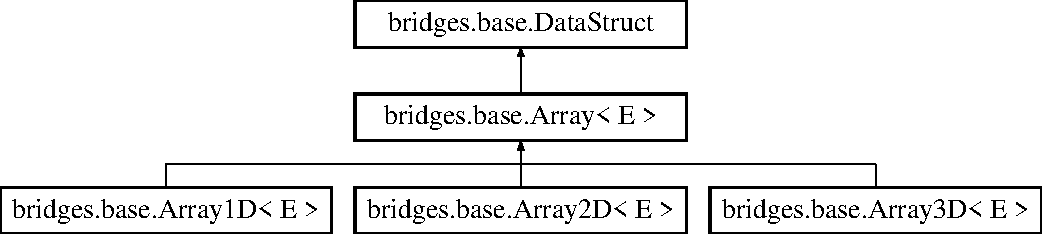
\includegraphics[height=3.000000cm]{classbridges_1_1base_1_1_array}
\end{center}
\end{figure}


\subsection{Detailed Description}
This class can be used to create arrays of type Element$<$\+E$>$. 

\begin{DoxyAuthor}{Author}
Kalpathi Subramanian
\end{DoxyAuthor}
\begin{DoxyDate}{Date}
10/8/16, 5/17/17, 5/30/18
\end{DoxyDate}
This class can be used to create arrays of type Element$<$\+E$>$ where E is a generic object representing application specific data.

This class is not directly called; instead use subclasses of arrays to construct arrays, depending on their dimension.

Arrays are internally represented as 1D arrays; currently 1D, 2D and 3D arrays are supported.


\begin{DoxyParams}{Parameters}
{\em $<$\+E$>$} & The generic parameter object that is part of this element, representing application specific data.\\
\hline
\end{DoxyParams}
\begin{DoxySeeAlso}{See also}
Example Tutorial at ~\newline
 \href{http://bridgesuncc.github.io/tutorials/Array.html}{\tt http\+://bridgesuncc.\+github.\+io/tutorials/\+Array.\+html} (1D, 2D, and 3D \hyperlink{classbridges_1_1base_1_1_array}{Array})~\newline
 
\end{DoxySeeAlso}
\subsection*{Public Member Functions}
\begin{DoxyCompactItemize}
\item 
\hyperlink{classbridges_1_1base_1_1_array_ad5dbf7bbd9811c2dac16a5c135465d4b}{Array} ()
\item 
\hyperlink{classbridges_1_1base_1_1_array_ab37dbe6efe0c34242456971e430763f7}{Array} (int num\+\_\+dims, int\mbox{[}$\,$\mbox{]} dims)
\item 
String \hyperlink{classbridges_1_1base_1_1_array_ad138b9787d46d053d6bd324b344be9a6}{get\+Data\+Struct\+Type} ()
\item 
void \hyperlink{classbridges_1_1base_1_1_array_ab7859668a25d16adfdb308e24c7d44c6}{set\+Num\+Dimensions} (int nd)
\item 
int \hyperlink{classbridges_1_1base_1_1_array_a808da9a62df3f0e7a905ec895a82087a}{get\+Num\+Dimensions} ()
\item 
void \hyperlink{classbridges_1_1base_1_1_array_aa357b6b957eeedfdb5acc9d653d7260f}{set\+Size} (int nd, int\mbox{[}$\,$\mbox{]} dim)
\begin{DoxyCompactList}\small\item\em Set the size of each dimensions; also allocates array space. \end{DoxyCompactList}\item 
void \hyperlink{classbridges_1_1base_1_1_array_af7aa7f3f18989af5f48a2b69cb7fb07d}{get\+Dimensions} (int\mbox{[}$\,$\mbox{]} dim)
\begin{DoxyCompactList}\small\item\em Get the size of each dimensions;. \end{DoxyCompactList}\item 
int \hyperlink{classbridges_1_1base_1_1_array_a49a3a4ea72c8315f1f14eed25071d18a}{get\+Size} ()
\item 
String \hyperlink{classbridges_1_1base_1_1_array_a111592e8b75202064bdf06d9c2234d74}{get\+Data\+Structure\+Representation} ()
\end{DoxyCompactItemize}
\subsection*{Protected Member Functions}
\begin{DoxyCompactItemize}
\item 
\hyperlink{classbridges_1_1base_1_1_element}{Element}$<$ E $>$ \hyperlink{classbridges_1_1base_1_1_array_a0e690cbe2606e44cce99b56802b63e0e}{get\+Element} (int indx)
\item 
void \hyperlink{classbridges_1_1base_1_1_array_aafde1304d602e8b0f673dd61bc00c18f}{set\+Element} (int indx, \hyperlink{classbridges_1_1base_1_1_element}{Element}$<$ E $>$ el)
\end{DoxyCompactItemize}
\subsection*{Additional Inherited Members}


\subsection{Constructor \& Destructor Documentation}
\mbox{\Hypertarget{classbridges_1_1base_1_1_array_ad5dbf7bbd9811c2dac16a5c135465d4b}\label{classbridges_1_1base_1_1_array_ad5dbf7bbd9811c2dac16a5c135465d4b}} 
\index{bridges\+::base\+::\+Array@{bridges\+::base\+::\+Array}!Array@{Array}}
\index{Array@{Array}!bridges\+::base\+::\+Array@{bridges\+::base\+::\+Array}}
\subsubsection{\texorpdfstring{Array()}{Array()}\hspace{0.1cm}{\footnotesize\ttfamily [1/2]}}
{\footnotesize\ttfamily \hyperlink{classbridges_1_1base_1_1_array}{bridges.\+base.\+Array}$<$ E $>$.\hyperlink{classbridges_1_1base_1_1_array}{Array} (\begin{DoxyParamCaption}{ }\end{DoxyParamCaption})}

\mbox{\Hypertarget{classbridges_1_1base_1_1_array_ab37dbe6efe0c34242456971e430763f7}\label{classbridges_1_1base_1_1_array_ab37dbe6efe0c34242456971e430763f7}} 
\index{bridges\+::base\+::\+Array@{bridges\+::base\+::\+Array}!Array@{Array}}
\index{Array@{Array}!bridges\+::base\+::\+Array@{bridges\+::base\+::\+Array}}
\subsubsection{\texorpdfstring{Array()}{Array()}\hspace{0.1cm}{\footnotesize\ttfamily [2/2]}}
{\footnotesize\ttfamily \hyperlink{classbridges_1_1base_1_1_array}{bridges.\+base.\+Array}$<$ E $>$.\hyperlink{classbridges_1_1base_1_1_array}{Array} (\begin{DoxyParamCaption}\item[{int}]{num\+\_\+dims,  }\item[{int \mbox{[}$\,$\mbox{]}}]{dims }\end{DoxyParamCaption})}

Create an array object with the specified dimensions


\begin{DoxyParams}{Parameters}
{\em num\+\_\+dims} & number of dimensions of the array \\
\hline
{\em dims} & size of each dimension \\
\hline
\end{DoxyParams}


\subsection{Member Function Documentation}
\mbox{\Hypertarget{classbridges_1_1base_1_1_array_ad138b9787d46d053d6bd324b344be9a6}\label{classbridges_1_1base_1_1_array_ad138b9787d46d053d6bd324b344be9a6}} 
\index{bridges\+::base\+::\+Array@{bridges\+::base\+::\+Array}!get\+Data\+Struct\+Type@{get\+Data\+Struct\+Type}}
\index{get\+Data\+Struct\+Type@{get\+Data\+Struct\+Type}!bridges\+::base\+::\+Array@{bridges\+::base\+::\+Array}}
\subsubsection{\texorpdfstring{get\+Data\+Struct\+Type()}{getDataStructType()}}
{\footnotesize\ttfamily String \hyperlink{classbridges_1_1base_1_1_array}{bridges.\+base.\+Array}$<$ E $>$.get\+Data\+Struct\+Type (\begin{DoxyParamCaption}{ }\end{DoxyParamCaption})}

This method gets the data structure type

\begin{DoxyReturn}{Returns}
The date structure type as a string 
\end{DoxyReturn}
\mbox{\Hypertarget{classbridges_1_1base_1_1_array_a111592e8b75202064bdf06d9c2234d74}\label{classbridges_1_1base_1_1_array_a111592e8b75202064bdf06d9c2234d74}} 
\index{bridges\+::base\+::\+Array@{bridges\+::base\+::\+Array}!get\+Data\+Structure\+Representation@{get\+Data\+Structure\+Representation}}
\index{get\+Data\+Structure\+Representation@{get\+Data\+Structure\+Representation}!bridges\+::base\+::\+Array@{bridges\+::base\+::\+Array}}
\subsubsection{\texorpdfstring{get\+Data\+Structure\+Representation()}{getDataStructureRepresentation()}}
{\footnotesize\ttfamily String \hyperlink{classbridges_1_1base_1_1_array}{bridges.\+base.\+Array}$<$ E $>$.get\+Data\+Structure\+Representation (\begin{DoxyParamCaption}{ }\end{DoxyParamCaption})}

Gets the data structure representation of the array (as J\+S\+ON)

\begin{DoxyReturn}{Returns}
array representation as a J\+S\+ON 
\end{DoxyReturn}
\mbox{\Hypertarget{classbridges_1_1base_1_1_array_af7aa7f3f18989af5f48a2b69cb7fb07d}\label{classbridges_1_1base_1_1_array_af7aa7f3f18989af5f48a2b69cb7fb07d}} 
\index{bridges\+::base\+::\+Array@{bridges\+::base\+::\+Array}!get\+Dimensions@{get\+Dimensions}}
\index{get\+Dimensions@{get\+Dimensions}!bridges\+::base\+::\+Array@{bridges\+::base\+::\+Array}}
\subsubsection{\texorpdfstring{get\+Dimensions()}{getDimensions()}}
{\footnotesize\ttfamily void \hyperlink{classbridges_1_1base_1_1_array}{bridges.\+base.\+Array}$<$ E $>$.get\+Dimensions (\begin{DoxyParamCaption}\item[{int \mbox{[}$\,$\mbox{]}}]{dim }\end{DoxyParamCaption})}



Get the size of each dimensions;. 

\begin{DoxyReturn}{Returns}
dim\mbox{[}\mbox{]} size of each dimension is returned 
\end{DoxyReturn}
\mbox{\Hypertarget{classbridges_1_1base_1_1_array_a0e690cbe2606e44cce99b56802b63e0e}\label{classbridges_1_1base_1_1_array_a0e690cbe2606e44cce99b56802b63e0e}} 
\index{bridges\+::base\+::\+Array@{bridges\+::base\+::\+Array}!get\+Element@{get\+Element}}
\index{get\+Element@{get\+Element}!bridges\+::base\+::\+Array@{bridges\+::base\+::\+Array}}
\subsubsection{\texorpdfstring{get\+Element()}{getElement()}}
{\footnotesize\ttfamily \hyperlink{classbridges_1_1base_1_1_element}{Element}$<$E$>$ \hyperlink{classbridges_1_1base_1_1_array}{bridges.\+base.\+Array}$<$ E $>$.get\+Element (\begin{DoxyParamCaption}\item[{int}]{indx }\end{DoxyParamCaption})\hspace{0.3cm}{\ttfamily [protected]}}

Get the object at \textquotesingle{}indx\textquotesingle{}


\begin{DoxyParams}{Parameters}
{\em indx} & index into the array \\
\hline
\end{DoxyParams}
\begin{DoxyReturn}{Returns}
Element$<$\+E$>$ object at \textquotesingle{}indx\textquotesingle{} 
\end{DoxyReturn}
\mbox{\Hypertarget{classbridges_1_1base_1_1_array_a808da9a62df3f0e7a905ec895a82087a}\label{classbridges_1_1base_1_1_array_a808da9a62df3f0e7a905ec895a82087a}} 
\index{bridges\+::base\+::\+Array@{bridges\+::base\+::\+Array}!get\+Num\+Dimensions@{get\+Num\+Dimensions}}
\index{get\+Num\+Dimensions@{get\+Num\+Dimensions}!bridges\+::base\+::\+Array@{bridges\+::base\+::\+Array}}
\subsubsection{\texorpdfstring{get\+Num\+Dimensions()}{getNumDimensions()}}
{\footnotesize\ttfamily int \hyperlink{classbridges_1_1base_1_1_array}{bridges.\+base.\+Array}$<$ E $>$.get\+Num\+Dimensions (\begin{DoxyParamCaption}{ }\end{DoxyParamCaption})}

Get the number of dimensions of the array;

\begin{DoxyReturn}{Returns}
number of dimensions 
\end{DoxyReturn}
\mbox{\Hypertarget{classbridges_1_1base_1_1_array_a49a3a4ea72c8315f1f14eed25071d18a}\label{classbridges_1_1base_1_1_array_a49a3a4ea72c8315f1f14eed25071d18a}} 
\index{bridges\+::base\+::\+Array@{bridges\+::base\+::\+Array}!get\+Size@{get\+Size}}
\index{get\+Size@{get\+Size}!bridges\+::base\+::\+Array@{bridges\+::base\+::\+Array}}
\subsubsection{\texorpdfstring{get\+Size()}{getSize()}}
{\footnotesize\ttfamily int \hyperlink{classbridges_1_1base_1_1_array}{bridges.\+base.\+Array}$<$ E $>$.get\+Size (\begin{DoxyParamCaption}{ }\end{DoxyParamCaption})}

Get the array size

\begin{DoxyReturn}{Returns}
size of the array 
\end{DoxyReturn}
\mbox{\Hypertarget{classbridges_1_1base_1_1_array_aafde1304d602e8b0f673dd61bc00c18f}\label{classbridges_1_1base_1_1_array_aafde1304d602e8b0f673dd61bc00c18f}} 
\index{bridges\+::base\+::\+Array@{bridges\+::base\+::\+Array}!set\+Element@{set\+Element}}
\index{set\+Element@{set\+Element}!bridges\+::base\+::\+Array@{bridges\+::base\+::\+Array}}
\subsubsection{\texorpdfstring{set\+Element()}{setElement()}}
{\footnotesize\ttfamily void \hyperlink{classbridges_1_1base_1_1_array}{bridges.\+base.\+Array}$<$ E $>$.set\+Element (\begin{DoxyParamCaption}\item[{int}]{indx,  }\item[{\hyperlink{classbridges_1_1base_1_1_element}{Element}$<$ E $>$}]{el }\end{DoxyParamCaption})\hspace{0.3cm}{\ttfamily [protected]}}

Set the input object at \textquotesingle{}indx\textquotesingle{} -\/ for 1D array


\begin{DoxyParams}{Parameters}
{\em indx} & index into the array \\
\hline
{\em el} & element object to be assigned at \textquotesingle{}indx\textquotesingle{} \\
\hline
\end{DoxyParams}
\mbox{\Hypertarget{classbridges_1_1base_1_1_array_ab7859668a25d16adfdb308e24c7d44c6}\label{classbridges_1_1base_1_1_array_ab7859668a25d16adfdb308e24c7d44c6}} 
\index{bridges\+::base\+::\+Array@{bridges\+::base\+::\+Array}!set\+Num\+Dimensions@{set\+Num\+Dimensions}}
\index{set\+Num\+Dimensions@{set\+Num\+Dimensions}!bridges\+::base\+::\+Array@{bridges\+::base\+::\+Array}}
\subsubsection{\texorpdfstring{set\+Num\+Dimensions()}{setNumDimensions()}}
{\footnotesize\ttfamily void \hyperlink{classbridges_1_1base_1_1_array}{bridges.\+base.\+Array}$<$ E $>$.set\+Num\+Dimensions (\begin{DoxyParamCaption}\item[{int}]{nd }\end{DoxyParamCaption})}

Set the number of dimensions of the array;


\begin{DoxyParams}{Parameters}
{\em nd} & number of dimensions \\
\hline
\end{DoxyParams}
\mbox{\Hypertarget{classbridges_1_1base_1_1_array_aa357b6b957eeedfdb5acc9d653d7260f}\label{classbridges_1_1base_1_1_array_aa357b6b957eeedfdb5acc9d653d7260f}} 
\index{bridges\+::base\+::\+Array@{bridges\+::base\+::\+Array}!set\+Size@{set\+Size}}
\index{set\+Size@{set\+Size}!bridges\+::base\+::\+Array@{bridges\+::base\+::\+Array}}
\subsubsection{\texorpdfstring{set\+Size()}{setSize()}}
{\footnotesize\ttfamily void \hyperlink{classbridges_1_1base_1_1_array}{bridges.\+base.\+Array}$<$ E $>$.set\+Size (\begin{DoxyParamCaption}\item[{int}]{nd,  }\item[{int \mbox{[}$\,$\mbox{]}}]{dim }\end{DoxyParamCaption})}



Set the size of each dimensions; also allocates array space. 


\begin{DoxyParams}{Parameters}
{\em nd} & number of dimension \\
\hline
{\em dim} & size of each dimension \\
\hline
\end{DoxyParams}


The documentation for this class was generated from the following file\+:\begin{DoxyCompactItemize}
\item 
/home/erik/work/bridges/bridges-\/java/src/main/java/bridges/base/\hyperlink{_array_8java}{Array.\+java}\end{DoxyCompactItemize}

\hypertarget{classbridges_1_1base_1_1_array1_d}{}\section{bridges.\+base.\+Array1D$<$ E $>$ Class Template Reference}
\label{classbridges_1_1base_1_1_array1_d}\index{bridges.\+base.\+Array1\+D$<$ E $>$@{bridges.\+base.\+Array1\+D$<$ E $>$}}
Inheritance diagram for bridges.\+base.\+Array1D$<$ E $>$\+:\begin{figure}[H]
\begin{center}
\leavevmode
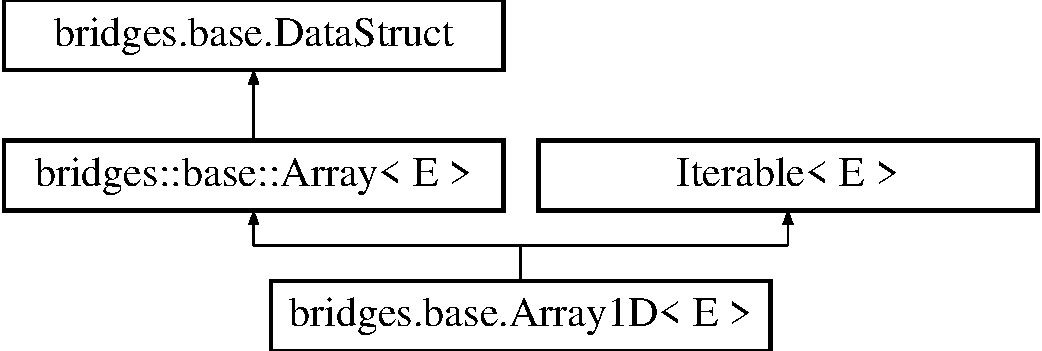
\includegraphics[height=3.000000cm]{classbridges_1_1base_1_1_array1_d}
\end{center}
\end{figure}


\subsection{Detailed Description}
This is a class can be used to create 1 dimensional arrays of type Element$<$\+E$>$. 

\begin{DoxyAuthor}{Author}
Kalpathi Subramanian
\end{DoxyAuthor}
\begin{DoxyDate}{Date}
7/18/19
\end{DoxyDate}
This class can be used to create 1D arrays of type Element$<$\+E$>$ where E is a generic object representing application specific data.

\mbox{\hyperlink{classbridges_1_1base_1_1_array1_d}{Array1D}} has iterator semantic to enable range for loops. For instance,


\begin{DoxyCode}
Array1D<Integer> arr = something();
\textcolor{keywordflow}{for} (Integer i : arr)
  System.out.println(i);
\end{DoxyCode}



\begin{DoxyParams}{Parameters}
{\em $<$\+E$>$} & The generic parameter object that is part of this element, representing application specific data.\\
\hline
\end{DoxyParams}
\begin{DoxySeeAlso}{See also}
Example Tutorial at ~\newline
 \href{http://bridgesuncc.github.io/tutorials/Array.html}{\tt http\+://bridgesuncc.\+github.\+io/tutorials/\+Array.\+html} (1D, 2D, and 3D \mbox{\hyperlink{classbridges_1_1base_1_1_array}{Array}})~\newline
 
\end{DoxySeeAlso}
\subsection*{Public Member Functions}
\begin{DoxyCompactItemize}
\item 
\mbox{\hyperlink{classbridges_1_1base_1_1_array1_d_a6554a5e9d23c1f11ad67498545f99d95}{Array1D}} ()
\item 
\mbox{\hyperlink{classbridges_1_1base_1_1_array1_d_a80d42f7bf54c865988ef7d02e46951cd}{Array1D}} (int sz)
\item 
\mbox{\hyperlink{classbridges_1_1base_1_1_element}{Element}}$<$ E $>$ \mbox{\hyperlink{classbridges_1_1base_1_1_array1_d_abc1cd5b4fb76bac80ab9a640a083dc25}{get\+Element}} (int indx)
\item 
void \mbox{\hyperlink{classbridges_1_1base_1_1_array1_d_ac749a6d97307998a2b37773456aca0fe}{set\+Element}} (int indx, \mbox{\hyperlink{classbridges_1_1base_1_1_element}{Element}}$<$ E $>$ el)
\item 
Iterator$<$ E $>$ \mbox{\hyperlink{classbridges_1_1base_1_1_array1_d_aed723a9f55895c1673e73cb818be7c15}{iterator}} ()
\end{DoxyCompactItemize}
\subsection*{Additional Inherited Members}


\subsection{Constructor \& Destructor Documentation}
\mbox{\Hypertarget{classbridges_1_1base_1_1_array1_d_a6554a5e9d23c1f11ad67498545f99d95}\label{classbridges_1_1base_1_1_array1_d_a6554a5e9d23c1f11ad67498545f99d95}} 
\index{bridges\+::base\+::\+Array1D@{bridges\+::base\+::\+Array1D}!Array1D@{Array1D}}
\index{Array1D@{Array1D}!bridges\+::base\+::\+Array1D@{bridges\+::base\+::\+Array1D}}
\subsubsection{\texorpdfstring{Array1\+D()}{Array1D()}\hspace{0.1cm}{\footnotesize\ttfamily [1/2]}}
{\footnotesize\ttfamily \mbox{\hyperlink{classbridges_1_1base_1_1_array1_d}{bridges.\+base.\+Array1D}}$<$ E $>$.\mbox{\hyperlink{classbridges_1_1base_1_1_array1_d}{Array1D}} (\begin{DoxyParamCaption}{ }\end{DoxyParamCaption})}

\mbox{\Hypertarget{classbridges_1_1base_1_1_array1_d_a80d42f7bf54c865988ef7d02e46951cd}\label{classbridges_1_1base_1_1_array1_d_a80d42f7bf54c865988ef7d02e46951cd}} 
\index{bridges\+::base\+::\+Array1D@{bridges\+::base\+::\+Array1D}!Array1D@{Array1D}}
\index{Array1D@{Array1D}!bridges\+::base\+::\+Array1D@{bridges\+::base\+::\+Array1D}}
\subsubsection{\texorpdfstring{Array1\+D()}{Array1D()}\hspace{0.1cm}{\footnotesize\ttfamily [2/2]}}
{\footnotesize\ttfamily \mbox{\hyperlink{classbridges_1_1base_1_1_array1_d}{bridges.\+base.\+Array1D}}$<$ E $>$.\mbox{\hyperlink{classbridges_1_1base_1_1_array1_d}{Array1D}} (\begin{DoxyParamCaption}\item[{int}]{sz }\end{DoxyParamCaption})}

Create a 1D array object


\begin{DoxyParams}{Parameters}
{\em sz} & number of elements in the array \\
\hline
\end{DoxyParams}


\subsection{Member Function Documentation}
\mbox{\Hypertarget{classbridges_1_1base_1_1_array1_d_abc1cd5b4fb76bac80ab9a640a083dc25}\label{classbridges_1_1base_1_1_array1_d_abc1cd5b4fb76bac80ab9a640a083dc25}} 
\index{bridges\+::base\+::\+Array1D@{bridges\+::base\+::\+Array1D}!get\+Element@{get\+Element}}
\index{get\+Element@{get\+Element}!bridges\+::base\+::\+Array1D@{bridges\+::base\+::\+Array1D}}
\subsubsection{\texorpdfstring{get\+Element()}{getElement()}}
{\footnotesize\ttfamily \mbox{\hyperlink{classbridges_1_1base_1_1_element}{Element}}$<$E$>$ \mbox{\hyperlink{classbridges_1_1base_1_1_array1_d}{bridges.\+base.\+Array1D}}$<$ E $>$.get\+Element (\begin{DoxyParamCaption}\item[{int}]{indx }\end{DoxyParamCaption})}

Get the object at \textquotesingle{}indx\textquotesingle{}


\begin{DoxyParams}{Parameters}
{\em indx} & index into the array \\
\hline
\end{DoxyParams}
\begin{DoxyReturn}{Returns}
Element$<$\+E$>$ object at \textquotesingle{}indx\textquotesingle{} 
\end{DoxyReturn}
\mbox{\Hypertarget{classbridges_1_1base_1_1_array1_d_aed723a9f55895c1673e73cb818be7c15}\label{classbridges_1_1base_1_1_array1_d_aed723a9f55895c1673e73cb818be7c15}} 
\index{bridges\+::base\+::\+Array1D@{bridges\+::base\+::\+Array1D}!iterator@{iterator}}
\index{iterator@{iterator}!bridges\+::base\+::\+Array1D@{bridges\+::base\+::\+Array1D}}
\subsubsection{\texorpdfstring{iterator()}{iterator()}}
{\footnotesize\ttfamily Iterator$<$E$>$ \mbox{\hyperlink{classbridges_1_1base_1_1_array1_d}{bridges.\+base.\+Array1D}}$<$ E $>$.iterator (\begin{DoxyParamCaption}{ }\end{DoxyParamCaption})}

\mbox{\Hypertarget{classbridges_1_1base_1_1_array1_d_ac749a6d97307998a2b37773456aca0fe}\label{classbridges_1_1base_1_1_array1_d_ac749a6d97307998a2b37773456aca0fe}} 
\index{bridges\+::base\+::\+Array1D@{bridges\+::base\+::\+Array1D}!set\+Element@{set\+Element}}
\index{set\+Element@{set\+Element}!bridges\+::base\+::\+Array1D@{bridges\+::base\+::\+Array1D}}
\subsubsection{\texorpdfstring{set\+Element()}{setElement()}}
{\footnotesize\ttfamily void \mbox{\hyperlink{classbridges_1_1base_1_1_array1_d}{bridges.\+base.\+Array1D}}$<$ E $>$.set\+Element (\begin{DoxyParamCaption}\item[{int}]{indx,  }\item[{\mbox{\hyperlink{classbridges_1_1base_1_1_element}{Element}}$<$ E $>$}]{el }\end{DoxyParamCaption})}

Set the input object at \textquotesingle{}indx\textquotesingle{} -\/ for 1D array


\begin{DoxyParams}{Parameters}
{\em indx} & index into the array \\
\hline
{\em el} & element object to be assigned at \textquotesingle{}indx\textquotesingle{} \\
\hline
\end{DoxyParams}


The documentation for this class was generated from the following file\+:\begin{DoxyCompactItemize}
\item 
/\+Users/kalpathi/gr/bridges/client/java/src/main/java/bridges/base/\mbox{\hyperlink{_array1_d_8java}{Array1\+D.\+java}}\end{DoxyCompactItemize}

\hypertarget{classbridges_1_1base_1_1_array2_d}{}\doxysection{bridges.\+base.\+Array2D$<$ E $>$ Class Template Reference}
\label{classbridges_1_1base_1_1_array2_d}\index{bridges.base.Array2D$<$ E $>$@{bridges.base.Array2D$<$ E $>$}}
Inheritance diagram for bridges.\+base.\+Array2D$<$ E $>$\+:\begin{figure}[H]
\begin{center}
\leavevmode
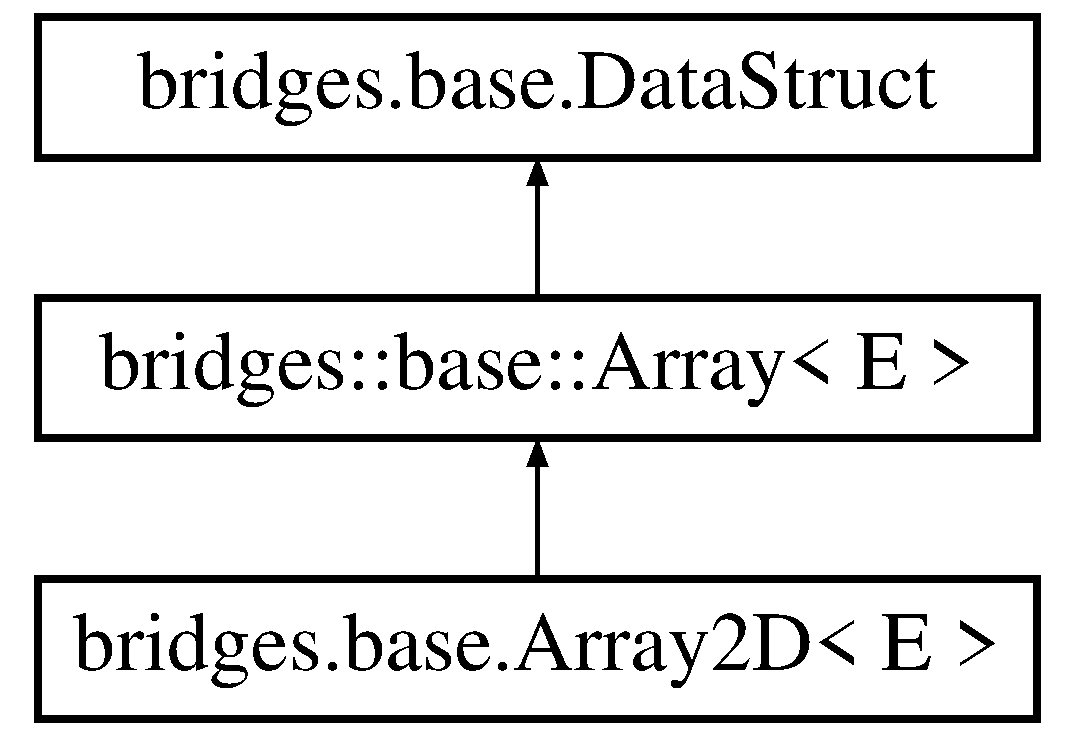
\includegraphics[height=3.000000cm]{classbridges_1_1base_1_1_array2_d}
\end{center}
\end{figure}


\doxysubsection{Detailed Description}
This class can be used to create arrays of type Element$<$\+E$>$. 

\begin{DoxyAuthor}{Author}
Kalpathi Subramanian
\end{DoxyAuthor}
\begin{DoxyDate}{Date}
10/8/16, 5/17/17, 5/30/18
\end{DoxyDate}
This class can be used to create arrays of type Element$<$\+E$>$ where E is a generic object representing application specific data.

Arrays are internally represented as 1D arrays; currently 1D, 2D and 3D arrays are supported.


\begin{DoxyParams}{Parameters}
{\em $<$\+E$>$} & The generic parameter object that is part of this element, representing application specific data.\\
\hline
\end{DoxyParams}
\begin{DoxySeeAlso}{See also}
Example Tutorial at ~\newline
 \href{http://bridgesuncc.github.io/tutorials/Array.html}{\texttt{ http\+://bridgesuncc.\+github.\+io/tutorials/\+Array.\+html}} (1D, 2D, and 3D \mbox{\hyperlink{classbridges_1_1base_1_1_array}{Array}})~\newline
 
\end{DoxySeeAlso}
\doxysubsection*{Public Member Functions}
\begin{DoxyCompactItemize}
\item 
\mbox{\hyperlink{classbridges_1_1base_1_1_array2_d_a48259310b06b5e143cd3bbdfe480f4a0}{Array2D}} ()
\item 
\mbox{\hyperlink{classbridges_1_1base_1_1_array2_d_a51fab452b4705ce593199b90cee2a103}{Array2D}} (int rows, int cols)
\item 
\mbox{\hyperlink{classbridges_1_1base_1_1_element}{Element}}$<$ E $>$ \mbox{\hyperlink{classbridges_1_1base_1_1_array2_d_a592b728c34d26a16e25daa1549073f51}{get\+Element}} (int row, int col)
\item 
void \mbox{\hyperlink{classbridges_1_1base_1_1_array2_d_a4f29fd9f736fdf46988ef6b3400684c3}{set\+Element}} (int row, int col, \mbox{\hyperlink{classbridges_1_1base_1_1_element}{Element}}$<$ E $>$ el)
\end{DoxyCompactItemize}
\doxysubsection*{Additional Inherited Members}


\doxysubsection{Constructor \& Destructor Documentation}
\mbox{\Hypertarget{classbridges_1_1base_1_1_array2_d_a48259310b06b5e143cd3bbdfe480f4a0}\label{classbridges_1_1base_1_1_array2_d_a48259310b06b5e143cd3bbdfe480f4a0}} 
\index{bridges.base.Array2D$<$ E $>$@{bridges.base.Array2D$<$ E $>$}!Array2D@{Array2D}}
\index{Array2D@{Array2D}!bridges.base.Array2D$<$ E $>$@{bridges.base.Array2D$<$ E $>$}}
\doxysubsubsection{\texorpdfstring{Array2D()}{Array2D()}\hspace{0.1cm}{\footnotesize\ttfamily [1/2]}}
{\footnotesize\ttfamily \mbox{\hyperlink{classbridges_1_1base_1_1_array2_d}{bridges.\+base.\+Array2D}}$<$ E $>$.\mbox{\hyperlink{classbridges_1_1base_1_1_array2_d}{Array2D}} (\begin{DoxyParamCaption}{ }\end{DoxyParamCaption})}

\mbox{\Hypertarget{classbridges_1_1base_1_1_array2_d_a51fab452b4705ce593199b90cee2a103}\label{classbridges_1_1base_1_1_array2_d_a51fab452b4705ce593199b90cee2a103}} 
\index{bridges.base.Array2D$<$ E $>$@{bridges.base.Array2D$<$ E $>$}!Array2D@{Array2D}}
\index{Array2D@{Array2D}!bridges.base.Array2D$<$ E $>$@{bridges.base.Array2D$<$ E $>$}}
\doxysubsubsection{\texorpdfstring{Array2D()}{Array2D()}\hspace{0.1cm}{\footnotesize\ttfamily [2/2]}}
{\footnotesize\ttfamily \mbox{\hyperlink{classbridges_1_1base_1_1_array2_d}{bridges.\+base.\+Array2D}}$<$ E $>$.\mbox{\hyperlink{classbridges_1_1base_1_1_array2_d}{Array2D}} (\begin{DoxyParamCaption}\item[{int}]{rows,  }\item[{int}]{cols }\end{DoxyParamCaption})}

Create an array object with the specified dimensions


\begin{DoxyParams}{Parameters}
{\em rows,cols} & size of the array \\
\hline
\end{DoxyParams}


\doxysubsection{Member Function Documentation}
\mbox{\Hypertarget{classbridges_1_1base_1_1_array2_d_a592b728c34d26a16e25daa1549073f51}\label{classbridges_1_1base_1_1_array2_d_a592b728c34d26a16e25daa1549073f51}} 
\index{bridges.base.Array2D$<$ E $>$@{bridges.base.Array2D$<$ E $>$}!getElement@{getElement}}
\index{getElement@{getElement}!bridges.base.Array2D$<$ E $>$@{bridges.base.Array2D$<$ E $>$}}
\doxysubsubsection{\texorpdfstring{getElement()}{getElement()}}
{\footnotesize\ttfamily \mbox{\hyperlink{classbridges_1_1base_1_1_element}{Element}}$<$E$>$ \mbox{\hyperlink{classbridges_1_1base_1_1_array2_d}{bridges.\+base.\+Array2D}}$<$ E $>$.get\+Element (\begin{DoxyParamCaption}\item[{int}]{row,  }\item[{int}]{col }\end{DoxyParamCaption})}

Get the object at index x, y -- for 2D arrays


\begin{DoxyParams}{Parameters}
{\em row} & -\/ row index \\
\hline
{\em col} & -\/ column index \\
\hline
\end{DoxyParams}
\begin{DoxyReturn}{Returns}
Element$<$\+E$>$ object at x, y 
\end{DoxyReturn}
\mbox{\Hypertarget{classbridges_1_1base_1_1_array2_d_a4f29fd9f736fdf46988ef6b3400684c3}\label{classbridges_1_1base_1_1_array2_d_a4f29fd9f736fdf46988ef6b3400684c3}} 
\index{bridges.base.Array2D$<$ E $>$@{bridges.base.Array2D$<$ E $>$}!setElement@{setElement}}
\index{setElement@{setElement}!bridges.base.Array2D$<$ E $>$@{bridges.base.Array2D$<$ E $>$}}
\doxysubsubsection{\texorpdfstring{setElement()}{setElement()}}
{\footnotesize\ttfamily void \mbox{\hyperlink{classbridges_1_1base_1_1_array2_d}{bridges.\+base.\+Array2D}}$<$ E $>$.set\+Element (\begin{DoxyParamCaption}\item[{int}]{row,  }\item[{int}]{col,  }\item[{\mbox{\hyperlink{classbridges_1_1base_1_1_element}{Element}}$<$ E $>$}]{el }\end{DoxyParamCaption})}

Set the input object at x, y -\/ 2D arrays


\begin{DoxyParams}{Parameters}
{\em row} & row index into the array \\
\hline
{\em col} & index index into the array \\
\hline
{\em el} & element object to be assigned at \textquotesingle{}indx\textquotesingle{} \\
\hline
\end{DoxyParams}


The documentation for this class was generated from the following file\+:\begin{DoxyCompactItemize}
\item 
/\+Users/kalpathi/gr/bridges/client/java/src/main/java/bridges/base/\mbox{\hyperlink{_array2_d_8java}{Array2\+D.\+java}}\end{DoxyCompactItemize}

\hypertarget{classbridges_1_1base_1_1_array3_d}{}\section{bridges.\+base.\+Array3D$<$ E $>$ Class Template Reference}
\label{classbridges_1_1base_1_1_array3_d}\index{bridges.\+base.\+Array3\+D$<$ E $>$@{bridges.\+base.\+Array3\+D$<$ E $>$}}
Inheritance diagram for bridges.\+base.\+Array3D$<$ E $>$\+:\begin{figure}[H]
\begin{center}
\leavevmode
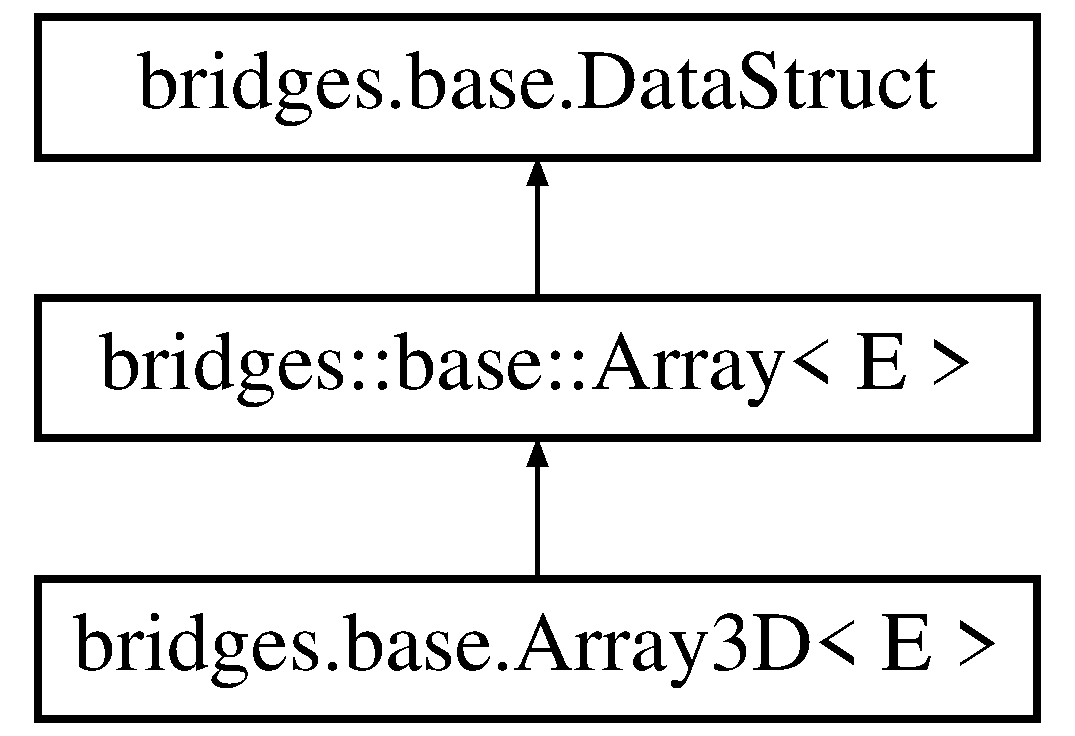
\includegraphics[height=3.000000cm]{classbridges_1_1base_1_1_array3_d}
\end{center}
\end{figure}


\subsection{Detailed Description}
This class can be used to create two dimensional arrays of type Element$<$\+E$>$. 

\begin{DoxyAuthor}{Author}
Kalpathi Subramanian
\end{DoxyAuthor}
\begin{DoxyDate}{Date}
7/18/19
\end{DoxyDate}
This class can be used to create three dimensional arrays of type Element$<$\+E$>$ where E is a generic object representing application specific data.

Arrays are internally represented as 1D arrays; currently 1D, 2D and 3D arrays are supported.


\begin{DoxyParams}{Parameters}
{\em $<$\+E$>$} & The generic parameter object that is part of this element, representing application specific data.\\
\hline
\end{DoxyParams}
\begin{DoxySeeAlso}{See also}
Example Tutorial at ~\newline
 \href{http://bridgesuncc.github.io/tutorials/Array.html}{\tt http\+://bridgesuncc.\+github.\+io/tutorials/\+Array.\+html} (1D, 2D, and 3D \hyperlink{classbridges_1_1base_1_1_array}{Array})~\newline
 
\end{DoxySeeAlso}
\subsection*{Public Member Functions}
\begin{DoxyCompactItemize}
\item 
\hyperlink{classbridges_1_1base_1_1_array3_d_a789f7fa8829d308b2d196dbd5b3f912f}{Array3D} ()
\item 
\hyperlink{classbridges_1_1base_1_1_array3_d_a015b271607e8b2b9e1425255f229af1b}{Array3D} (int\mbox{[}$\,$\mbox{]} dims)
\item 
\hyperlink{classbridges_1_1base_1_1_array3_d_a247f9b041470a190cdd63c2ff20c7aca}{Array3D} (int slices, int rows, int cols)
\item 
\hyperlink{classbridges_1_1base_1_1_element}{Element}$<$ E $>$ \hyperlink{classbridges_1_1base_1_1_array3_d_a2f157a0da356f83ff2d13fe72cabc9ad}{get\+Element} (int slice, int row, int col)
\item 
void \hyperlink{classbridges_1_1base_1_1_array3_d_a54caaf2a64906e7378a4049faec14750}{set\+Element} (int slice, int row, int col, \hyperlink{classbridges_1_1base_1_1_element}{Element}$<$ E $>$ el)
\end{DoxyCompactItemize}
\subsection*{Additional Inherited Members}


\subsection{Constructor \& Destructor Documentation}
\mbox{\Hypertarget{classbridges_1_1base_1_1_array3_d_a789f7fa8829d308b2d196dbd5b3f912f}\label{classbridges_1_1base_1_1_array3_d_a789f7fa8829d308b2d196dbd5b3f912f}} 
\index{bridges\+::base\+::\+Array3D@{bridges\+::base\+::\+Array3D}!Array3D@{Array3D}}
\index{Array3D@{Array3D}!bridges\+::base\+::\+Array3D@{bridges\+::base\+::\+Array3D}}
\subsubsection{\texorpdfstring{Array3\+D()}{Array3D()}\hspace{0.1cm}{\footnotesize\ttfamily [1/3]}}
{\footnotesize\ttfamily \hyperlink{classbridges_1_1base_1_1_array3_d}{bridges.\+base.\+Array3D}$<$ E $>$.\hyperlink{classbridges_1_1base_1_1_array3_d}{Array3D} (\begin{DoxyParamCaption}{ }\end{DoxyParamCaption})}

\mbox{\Hypertarget{classbridges_1_1base_1_1_array3_d_a015b271607e8b2b9e1425255f229af1b}\label{classbridges_1_1base_1_1_array3_d_a015b271607e8b2b9e1425255f229af1b}} 
\index{bridges\+::base\+::\+Array3D@{bridges\+::base\+::\+Array3D}!Array3D@{Array3D}}
\index{Array3D@{Array3D}!bridges\+::base\+::\+Array3D@{bridges\+::base\+::\+Array3D}}
\subsubsection{\texorpdfstring{Array3\+D()}{Array3D()}\hspace{0.1cm}{\footnotesize\ttfamily [2/3]}}
{\footnotesize\ttfamily \hyperlink{classbridges_1_1base_1_1_array3_d}{bridges.\+base.\+Array3D}$<$ E $>$.\hyperlink{classbridges_1_1base_1_1_array3_d}{Array3D} (\begin{DoxyParamCaption}\item[{int \mbox{[}$\,$\mbox{]}}]{dims }\end{DoxyParamCaption})}

Create an array object with the specified dimensions


\begin{DoxyParams}{Parameters}
{\em dims} & size of each dimension \\
\hline
\end{DoxyParams}
\mbox{\Hypertarget{classbridges_1_1base_1_1_array3_d_a247f9b041470a190cdd63c2ff20c7aca}\label{classbridges_1_1base_1_1_array3_d_a247f9b041470a190cdd63c2ff20c7aca}} 
\index{bridges\+::base\+::\+Array3D@{bridges\+::base\+::\+Array3D}!Array3D@{Array3D}}
\index{Array3D@{Array3D}!bridges\+::base\+::\+Array3D@{bridges\+::base\+::\+Array3D}}
\subsubsection{\texorpdfstring{Array3\+D()}{Array3D()}\hspace{0.1cm}{\footnotesize\ttfamily [3/3]}}
{\footnotesize\ttfamily \hyperlink{classbridges_1_1base_1_1_array3_d}{bridges.\+base.\+Array3D}$<$ E $>$.\hyperlink{classbridges_1_1base_1_1_array3_d}{Array3D} (\begin{DoxyParamCaption}\item[{int}]{slices,  }\item[{int}]{rows,  }\item[{int}]{cols }\end{DoxyParamCaption})}

Create an array object with the specified dimensions


\begin{DoxyParams}{Parameters}
{\em cols} & number of columns \\
\hline
{\em rows} & number of rows \\
\hline
{\em slices} & number of slices \\
\hline
\end{DoxyParams}


\subsection{Member Function Documentation}
\mbox{\Hypertarget{classbridges_1_1base_1_1_array3_d_a2f157a0da356f83ff2d13fe72cabc9ad}\label{classbridges_1_1base_1_1_array3_d_a2f157a0da356f83ff2d13fe72cabc9ad}} 
\index{bridges\+::base\+::\+Array3D@{bridges\+::base\+::\+Array3D}!get\+Element@{get\+Element}}
\index{get\+Element@{get\+Element}!bridges\+::base\+::\+Array3D@{bridges\+::base\+::\+Array3D}}
\subsubsection{\texorpdfstring{get\+Element()}{getElement()}}
{\footnotesize\ttfamily \hyperlink{classbridges_1_1base_1_1_element}{Element}$<$E$>$ \hyperlink{classbridges_1_1base_1_1_array3_d}{bridges.\+base.\+Array3D}$<$ E $>$.get\+Element (\begin{DoxyParamCaption}\item[{int}]{slice,  }\item[{int}]{row,  }\item[{int}]{col }\end{DoxyParamCaption})}

Get the object at slice, row, column -- for 3D arrays


\begin{DoxyParams}{Parameters}
{\em slice} & -\/ slice index \\
\hline
{\em row} & -\/ row index \\
\hline
{\em col} & -\/ column index\\
\hline
\end{DoxyParams}
\begin{DoxyReturn}{Returns}
Element$<$\+E$>$ object at slice, row, column 
\end{DoxyReturn}
\mbox{\Hypertarget{classbridges_1_1base_1_1_array3_d_a54caaf2a64906e7378a4049faec14750}\label{classbridges_1_1base_1_1_array3_d_a54caaf2a64906e7378a4049faec14750}} 
\index{bridges\+::base\+::\+Array3D@{bridges\+::base\+::\+Array3D}!set\+Element@{set\+Element}}
\index{set\+Element@{set\+Element}!bridges\+::base\+::\+Array3D@{bridges\+::base\+::\+Array3D}}
\subsubsection{\texorpdfstring{set\+Element()}{setElement()}}
{\footnotesize\ttfamily void \hyperlink{classbridges_1_1base_1_1_array3_d}{bridges.\+base.\+Array3D}$<$ E $>$.set\+Element (\begin{DoxyParamCaption}\item[{int}]{slice,  }\item[{int}]{row,  }\item[{int}]{col,  }\item[{\hyperlink{classbridges_1_1base_1_1_element}{Element}$<$ E $>$}]{el }\end{DoxyParamCaption})}

Set the input object at \textquotesingle{}col, row, slice\textquotesingle{}


\begin{DoxyParams}{Parameters}
{\em col} & column index into the array \\
\hline
{\em row} & row index into the array \\
\hline
{\em slice} & slice index into the array\\
\hline
{\em el} & element object to be assigned at \textquotesingle{}indx\textquotesingle{} \\
\hline
\end{DoxyParams}


The documentation for this class was generated from the following file\+:\begin{DoxyCompactItemize}
\item 
/home/erik/work/bridges/bridges-\/java/src/main/java/bridges/base/\hyperlink{_array3_d_8java}{Array3\+D.\+java}\end{DoxyCompactItemize}

\hypertarget{classbridges_1_1data__src__dependent_1_1_assignment}{}\section{bridges.\+data\+\_\+src\+\_\+dependent.\+Assignment Class Reference}
\label{classbridges_1_1data__src__dependent_1_1_assignment}\index{bridges.data\_src\_dependent.Assignment@{bridges.data\_src\_dependent.Assignment}}


Struct like class used to represent Bridges Assignments as they are returned from the server.  




Inherits bridges.\+data\+\_\+src\+\_\+dependent.\+Data\+Source.

\subsection*{Public Attributes}
\begin{DoxyCompactItemize}
\item 
String \mbox{\hyperlink{classbridges_1_1data__src__dependent_1_1_assignment_aa7326ba8e0eb02fff4e5b22e4b89e61d}{username}}
\item 
double \mbox{\hyperlink{classbridges_1_1data__src__dependent_1_1_assignment_a88c98da9e5ba6f8d83326d6fbae659d8}{assignment\+ID}}
\item 
\mbox{\hyperlink{classbridges_1_1data__src__dependent_1_1_assignment_data}{Assignment\+Data}} \mbox{[}$\,$\mbox{]} \mbox{\hyperlink{classbridges_1_1data__src__dependent_1_1_assignment_a23d503c5e6eae939bb8262dc8e18c259}{data}}
\end{DoxyCompactItemize}


\subsection{Detailed Description}
Struct like class used to represent Bridges Assignments as they are returned from the server. 

\begin{DoxyAuthor}{Author}
Alec Goncharow 
\end{DoxyAuthor}


\subsection{Member Data Documentation}
\mbox{\Hypertarget{classbridges_1_1data__src__dependent_1_1_assignment_a88c98da9e5ba6f8d83326d6fbae659d8}\label{classbridges_1_1data__src__dependent_1_1_assignment_a88c98da9e5ba6f8d83326d6fbae659d8}} 
\index{bridges.data\_src\_dependent.Assignment@{bridges.data\_src\_dependent.Assignment}!assignmentID@{assignmentID}}
\index{assignmentID@{assignmentID}!bridges.data\_src\_dependent.Assignment@{bridges.data\_src\_dependent.Assignment}}
\subsubsection{\texorpdfstring{assignmentID}{assignmentID}}
{\footnotesize\ttfamily double bridges.\+data\+\_\+src\+\_\+dependent.\+Assignment.\+assignment\+ID}

\mbox{\Hypertarget{classbridges_1_1data__src__dependent_1_1_assignment_a23d503c5e6eae939bb8262dc8e18c259}\label{classbridges_1_1data__src__dependent_1_1_assignment_a23d503c5e6eae939bb8262dc8e18c259}} 
\index{bridges.data\_src\_dependent.Assignment@{bridges.data\_src\_dependent.Assignment}!data@{data}}
\index{data@{data}!bridges.data\_src\_dependent.Assignment@{bridges.data\_src\_dependent.Assignment}}
\subsubsection{\texorpdfstring{data}{data}}
{\footnotesize\ttfamily \mbox{\hyperlink{classbridges_1_1data__src__dependent_1_1_assignment_data}{Assignment\+Data}} \mbox{[}$\,$\mbox{]} bridges.\+data\+\_\+src\+\_\+dependent.\+Assignment.\+data}

\mbox{\Hypertarget{classbridges_1_1data__src__dependent_1_1_assignment_aa7326ba8e0eb02fff4e5b22e4b89e61d}\label{classbridges_1_1data__src__dependent_1_1_assignment_aa7326ba8e0eb02fff4e5b22e4b89e61d}} 
\index{bridges.data\_src\_dependent.Assignment@{bridges.data\_src\_dependent.Assignment}!username@{username}}
\index{username@{username}!bridges.data\_src\_dependent.Assignment@{bridges.data\_src\_dependent.Assignment}}
\subsubsection{\texorpdfstring{username}{username}}
{\footnotesize\ttfamily String bridges.\+data\+\_\+src\+\_\+dependent.\+Assignment.\+username}



The documentation for this class was generated from the following file\+:\begin{DoxyCompactItemize}
\item 
/\+Users/kalpathi/gr/bridges/java/src/main/java/bridges/data\+\_\+src\+\_\+dependent/\mbox{\hyperlink{_assignment_8java}{Assignment.\+java}}\end{DoxyCompactItemize}

\hypertarget{classbridges_1_1data__src__dependent_1_1_assignment_data}{}\doxysection{bridges.\+data\+\_\+src\+\_\+dependent.\+Assignment\+Data Class Reference}
\label{classbridges_1_1data__src__dependent_1_1_assignment_data}\index{bridges.data\_src\_dependent.AssignmentData@{bridges.data\_src\_dependent.AssignmentData}}


\doxysubsection{Detailed Description}
Struct like class used to represent Bridges \mbox{\hyperlink{classbridges_1_1data__src__dependent_1_1_assignment}{Assignment}} Data as returned from the server. 

\begin{DoxyAuthor}{Author}
Alec Goncharow 
\end{DoxyAuthor}
\doxysubsection*{Public Attributes}
\begin{DoxyCompactItemize}
\item 
String \mbox{\hyperlink{classbridges_1_1data__src__dependent_1_1_assignment_data_a6734aba0f017aca0024fcd80905be4f4}{coord\+\_\+system\+\_\+type}}
\item 
Object \mbox{[}$\,$\mbox{]} \mbox{\hyperlink{classbridges_1_1data__src__dependent_1_1_assignment_data_a1d7c23816a57cf9b3bd1bc0b53f15e8e}{nodes}}
\item 
int \mbox{[}$\,$\mbox{]} \mbox{\hyperlink{classbridges_1_1data__src__dependent_1_1_assignment_data_ab4aa179a24395748542f6fb64307132c}{dimensions}}
\end{DoxyCompactItemize}


\doxysubsection{Member Data Documentation}
\mbox{\Hypertarget{classbridges_1_1data__src__dependent_1_1_assignment_data_a6734aba0f017aca0024fcd80905be4f4}\label{classbridges_1_1data__src__dependent_1_1_assignment_data_a6734aba0f017aca0024fcd80905be4f4}} 
\index{bridges.data\_src\_dependent.AssignmentData@{bridges.data\_src\_dependent.AssignmentData}!coord\_system\_type@{coord\_system\_type}}
\index{coord\_system\_type@{coord\_system\_type}!bridges.data\_src\_dependent.AssignmentData@{bridges.data\_src\_dependent.AssignmentData}}
\doxysubsubsection{\texorpdfstring{coord\_system\_type}{coord\_system\_type}}
{\footnotesize\ttfamily String bridges.\+data\+\_\+src\+\_\+dependent.\+Assignment\+Data.\+coord\+\_\+system\+\_\+type}

\mbox{\Hypertarget{classbridges_1_1data__src__dependent_1_1_assignment_data_ab4aa179a24395748542f6fb64307132c}\label{classbridges_1_1data__src__dependent_1_1_assignment_data_ab4aa179a24395748542f6fb64307132c}} 
\index{bridges.data\_src\_dependent.AssignmentData@{bridges.data\_src\_dependent.AssignmentData}!dimensions@{dimensions}}
\index{dimensions@{dimensions}!bridges.data\_src\_dependent.AssignmentData@{bridges.data\_src\_dependent.AssignmentData}}
\doxysubsubsection{\texorpdfstring{dimensions}{dimensions}}
{\footnotesize\ttfamily int \mbox{[}$\,$\mbox{]} bridges.\+data\+\_\+src\+\_\+dependent.\+Assignment\+Data.\+dimensions}

\mbox{\Hypertarget{classbridges_1_1data__src__dependent_1_1_assignment_data_a1d7c23816a57cf9b3bd1bc0b53f15e8e}\label{classbridges_1_1data__src__dependent_1_1_assignment_data_a1d7c23816a57cf9b3bd1bc0b53f15e8e}} 
\index{bridges.data\_src\_dependent.AssignmentData@{bridges.data\_src\_dependent.AssignmentData}!nodes@{nodes}}
\index{nodes@{nodes}!bridges.data\_src\_dependent.AssignmentData@{bridges.data\_src\_dependent.AssignmentData}}
\doxysubsubsection{\texorpdfstring{nodes}{nodes}}
{\footnotesize\ttfamily Object \mbox{[}$\,$\mbox{]} bridges.\+data\+\_\+src\+\_\+dependent.\+Assignment\+Data.\+nodes}



The documentation for this class was generated from the following file\+:\begin{DoxyCompactItemize}
\item 
/\+Users/kalpathi/gr/bridges/client/java/src/main/java/bridges/data\+\_\+src\+\_\+dependent/\mbox{\hyperlink{_assignment_data_8java}{Assignment\+Data.\+java}}\end{DoxyCompactItemize}

\hypertarget{classbridges_1_1base_1_1_audio_channel}{}\section{bridges.\+base.\+Audio\+Channel Class Reference}
\label{classbridges_1_1base_1_1_audio_channel}\index{bridges.\+base.\+Audio\+Channel@{bridges.\+base.\+Audio\+Channel}}


\subsection{Detailed Description}
This class provides support for audio A\+PI in bridges; this class stores the properties and audio data of a single channel. \subsection*{Public Member Functions}
\begin{DoxyCompactItemize}
\item 
\hyperlink{classbridges_1_1base_1_1_audio_channel_a1fb5be6b6ba3f393abedc7cd068e0c49}{Audio\+Channel} (int sample\+Count)
\begin{DoxyCompactList}\small\item\em constructore \end{DoxyCompactList}\item 
int \hyperlink{classbridges_1_1base_1_1_audio_channel_af367155c1e380bc7e934af74e74b0ef7}{get\+Channel\+Size} ()
\begin{DoxyCompactList}\small\item\em get sample count \end{DoxyCompactList}\item 
int \hyperlink{classbridges_1_1base_1_1_audio_channel_a62b3fdc6e9e03996f15216d5f7f2d3fb}{get\+Sample} (int index)
\begin{DoxyCompactList}\small\item\em get sample at an index in the array \end{DoxyCompactList}\item 
void \hyperlink{classbridges_1_1base_1_1_audio_channel_aea69a2dab1bb9cc8c930f476b8392fd9}{set\+Sample} (int index, int sample)
\begin{DoxyCompactList}\small\item\em set sample at an index in the array \end{DoxyCompactList}\end{DoxyCompactItemize}


\subsection{Constructor \& Destructor Documentation}
\mbox{\Hypertarget{classbridges_1_1base_1_1_audio_channel_a1fb5be6b6ba3f393abedc7cd068e0c49}\label{classbridges_1_1base_1_1_audio_channel_a1fb5be6b6ba3f393abedc7cd068e0c49}} 
\index{bridges\+::base\+::\+Audio\+Channel@{bridges\+::base\+::\+Audio\+Channel}!Audio\+Channel@{Audio\+Channel}}
\index{Audio\+Channel@{Audio\+Channel}!bridges\+::base\+::\+Audio\+Channel@{bridges\+::base\+::\+Audio\+Channel}}
\subsubsection{\texorpdfstring{Audio\+Channel()}{AudioChannel()}}
{\footnotesize\ttfamily bridges.\+base.\+Audio\+Channel.\+Audio\+Channel (\begin{DoxyParamCaption}\item[{int}]{sample\+Count }\end{DoxyParamCaption})}



constructore 


\begin{DoxyParams}{Parameters}
{\em sample\+Count} & number of samples \\
\hline
\end{DoxyParams}


\subsection{Member Function Documentation}
\mbox{\Hypertarget{classbridges_1_1base_1_1_audio_channel_af367155c1e380bc7e934af74e74b0ef7}\label{classbridges_1_1base_1_1_audio_channel_af367155c1e380bc7e934af74e74b0ef7}} 
\index{bridges\+::base\+::\+Audio\+Channel@{bridges\+::base\+::\+Audio\+Channel}!get\+Channel\+Size@{get\+Channel\+Size}}
\index{get\+Channel\+Size@{get\+Channel\+Size}!bridges\+::base\+::\+Audio\+Channel@{bridges\+::base\+::\+Audio\+Channel}}
\subsubsection{\texorpdfstring{get\+Channel\+Size()}{getChannelSize()}}
{\footnotesize\ttfamily int bridges.\+base.\+Audio\+Channel.\+get\+Channel\+Size (\begin{DoxyParamCaption}{ }\end{DoxyParamCaption})}



get sample count 

\begin{DoxyReturn}{Returns}
number of samples 
\end{DoxyReturn}
\mbox{\Hypertarget{classbridges_1_1base_1_1_audio_channel_a62b3fdc6e9e03996f15216d5f7f2d3fb}\label{classbridges_1_1base_1_1_audio_channel_a62b3fdc6e9e03996f15216d5f7f2d3fb}} 
\index{bridges\+::base\+::\+Audio\+Channel@{bridges\+::base\+::\+Audio\+Channel}!get\+Sample@{get\+Sample}}
\index{get\+Sample@{get\+Sample}!bridges\+::base\+::\+Audio\+Channel@{bridges\+::base\+::\+Audio\+Channel}}
\subsubsection{\texorpdfstring{get\+Sample()}{getSample()}}
{\footnotesize\ttfamily int bridges.\+base.\+Audio\+Channel.\+get\+Sample (\begin{DoxyParamCaption}\item[{int}]{index }\end{DoxyParamCaption})}



get sample at an index in the array 


\begin{DoxyParams}{Parameters}
{\em index} & to look for sample \\
\hline
\end{DoxyParams}
\mbox{\Hypertarget{classbridges_1_1base_1_1_audio_channel_aea69a2dab1bb9cc8c930f476b8392fd9}\label{classbridges_1_1base_1_1_audio_channel_aea69a2dab1bb9cc8c930f476b8392fd9}} 
\index{bridges\+::base\+::\+Audio\+Channel@{bridges\+::base\+::\+Audio\+Channel}!set\+Sample@{set\+Sample}}
\index{set\+Sample@{set\+Sample}!bridges\+::base\+::\+Audio\+Channel@{bridges\+::base\+::\+Audio\+Channel}}
\subsubsection{\texorpdfstring{set\+Sample()}{setSample()}}
{\footnotesize\ttfamily void bridges.\+base.\+Audio\+Channel.\+set\+Sample (\begin{DoxyParamCaption}\item[{int}]{index,  }\item[{int}]{sample }\end{DoxyParamCaption})}



set sample at an index in the array 


\begin{DoxyParams}{Parameters}
{\em index} & \\
\hline
{\em sample} & sample data \\
\hline
\end{DoxyParams}


The documentation for this class was generated from the following file\+:\begin{DoxyCompactItemize}
\item 
/home/erik/work/bridges/bridges-\/java/src/main/java/bridges/base/\hyperlink{_audio_channel_8java}{Audio\+Channel.\+java}\end{DoxyCompactItemize}

\hypertarget{classbridges_1_1base_1_1_audio_clip}{}\section{bridges.\+base.\+Audio\+Clip Class Reference}
\label{classbridges_1_1base_1_1_audio_clip}\index{bridges.\+base.\+Audio\+Clip@{bridges.\+base.\+Audio\+Clip}}
Inheritance diagram for bridges.\+base.\+Audio\+Clip\+:\begin{figure}[H]
\begin{center}
\leavevmode
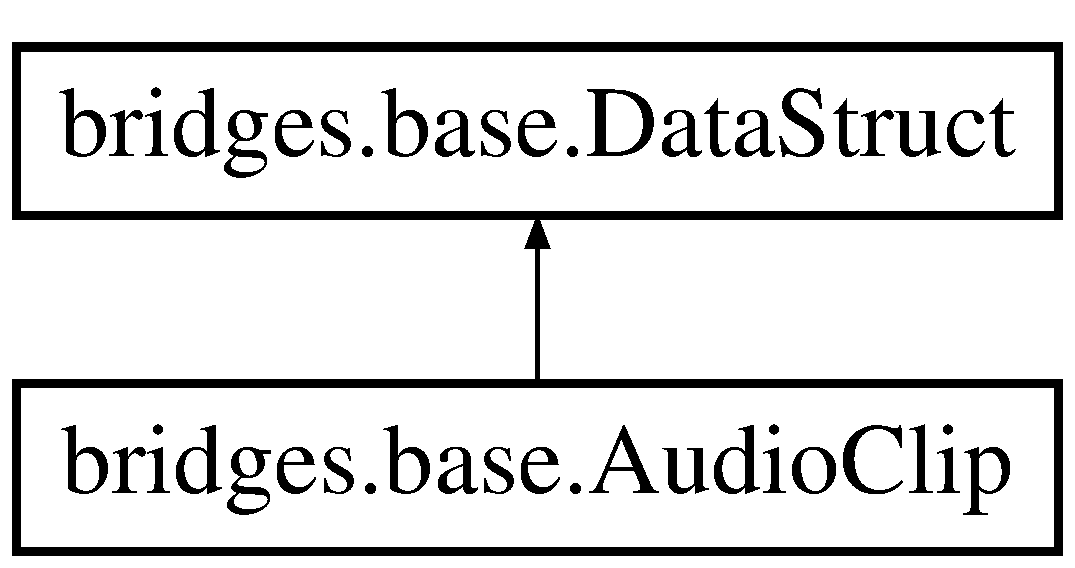
\includegraphics[height=2.000000cm]{classbridges_1_1base_1_1_audio_clip}
\end{center}
\end{figure}


\subsection{Detailed Description}
This class provides support for reading, modifying, and playing, audio waveform. 

This class provides a way to represent an \hyperlink{classbridges_1_1base_1_1_audio_clip}{Audio\+Clip} (think of a .W\+AV file) in Bridges as waveforms.

An \hyperlink{classbridges_1_1base_1_1_audio_clip}{Audio\+Clip} can be composed of multiple channels\+: a stereo sound would be composed of 2 channels (Left and Right), a mono sound would be composed of a single channel. A 5.\+1 sound would be composed of 6 channels. When building an \hyperlink{classbridges_1_1base_1_1_audio_clip}{Audio\+Clip} from a file, the number of channels is taken from the file; some constructors have a num\+Channels that enables to pass the number of channels explicitly. If unsure, one can know how many channels are in an audio clip using \hyperlink{classbridges_1_1base_1_1_audio_clip_a09e8b5da5249851f7583e910f24b0395}{get\+Num\+Channels()}.

Each channel is essentially a 1D signal. That is to say, it is an array of values that represent how far the membrane of a speaker should be from its resting position. The quality of the sound is controlled by two parameters\+: sampling rate and sampling depth.

Sampling rate tells how many positions per second are encoded by the \hyperlink{classbridges_1_1base_1_1_audio_clip}{Audio\+Clip}. It is expressed in Hertz. CD quality is 44100\+Hz; while walkie-\/talkies use 8000\+Hz. It is set automatically if read from a file; or it can be passed as the sample\+Rate parameter to some of the constructors. The sampling rate can be obtained from an \hyperlink{classbridges_1_1base_1_1_audio_clip}{Audio\+Clip} using \hyperlink{classbridges_1_1base_1_1_audio_clip_a610df43929946a6186e6739e361916eb}{get\+Sample\+Rate()}.

The length of an \hyperlink{classbridges_1_1base_1_1_audio_clip}{Audio\+Clip} is expressed in number of samples. So if an \hyperlink{classbridges_1_1base_1_1_audio_clip}{Audio\+Clip} is composed of 16,000 samples with a sampling rate of 8000\+Hz, the clip would be 2 seconds long. The number of samples can obtained with \hyperlink{classbridges_1_1base_1_1_audio_clip_a8ad739b7a085787028b4278d65b1b3f4}{get\+Sample\+Count()}; it is set from a file or can be passed as the sample\+Count parameter of some of the constructor.

The sampling depth indicates how many different positions the membrane can take. It is typically expressed in bits with supported values being 8-\/bit, 16-\/bit, 24-\/bit, and 32-\/bit. If a clip is encoded with a depth of 8 bits, the membrane can take 2$^\wedge$8 different position ranging from -\/128 to +127, with 0 being the resting position. The sampling depth is read from files or passed as the sample\+Bits parameter of the constructor. The sampling depth of an existing clip can be obtained with \hyperlink{classbridges_1_1base_1_1_audio_clip_a59e5a3f38768e52c15e43b5679f3f09c}{get\+Sample\+Bits()}.

The individual samples are accessed with the \hyperlink{classbridges_1_1base_1_1_audio_clip_a0db520ed7ad301161e03a55b783856f8}{get\+Sample()} and \hyperlink{classbridges_1_1base_1_1_audio_clip_a896e82f2788b319569c4f0e8f919ffc9}{set\+Sample()} functions. The samples are integer values in the \mbox{[}-\/2$^\wedge$(\hyperlink{classbridges_1_1base_1_1_audio_clip_a59e5a3f38768e52c15e43b5679f3f09c}{get\+Sample\+Bits()}-\/1) ; 2$^\wedge$(\hyperlink{classbridges_1_1base_1_1_audio_clip_a59e5a3f38768e52c15e43b5679f3f09c}{get\+Sample\+Bits()}-\/1)\mbox{[} range. The functions allow to specify for channel and sample index. \subsection*{Public Member Functions}
\begin{DoxyCompactItemize}
\item 
\hyperlink{classbridges_1_1base_1_1_audio_clip_a83e87997fd53dbcbde7680b90c1ff3f2}{Audio\+Clip} (int sample\+Count, int num\+Channels, int sample\+Bits, int sample\+Rate)
\begin{DoxyCompactList}\small\item\em create an audio clip \end{DoxyCompactList}\item 
\hyperlink{classbridges_1_1base_1_1_audio_clip_aece4ed61f09688a54e636ce3dc206239}{Audio\+Clip} (Wav\+File wav\+File)  throws I\+O\+Exception
\begin{DoxyCompactList}\small\item\em create an audio clip from a Wav\+File object \end{DoxyCompactList}\item 
\hyperlink{classbridges_1_1base_1_1_audio_clip_a70d5f6f10dad6da2f27bb04b7021e2fa}{Audio\+Clip} (String file)  throws I\+O\+Exception 
\begin{DoxyCompactList}\small\item\em create an audio clip from a File \end{DoxyCompactList}\item 
\hyperlink{classbridges_1_1base_1_1_audio_clip_aca2a5258c29b104bf8216ae5ec3c5938}{Audio\+Clip} (int sample\+Count, int num\+Channels)
\begin{DoxyCompactList}\small\item\em create an audio clip \end{DoxyCompactList}\item 
int \hyperlink{classbridges_1_1base_1_1_audio_clip_a09e8b5da5249851f7583e910f24b0395}{get\+Num\+Channels} ()
\begin{DoxyCompactList}\small\item\em returns the number of channels of the clip \end{DoxyCompactList}\item 
int \hyperlink{classbridges_1_1base_1_1_audio_clip_a610df43929946a6186e6739e361916eb}{get\+Sample\+Rate} ()
\begin{DoxyCompactList}\small\item\em returns the sampling rate of the clip \end{DoxyCompactList}\item 
int \hyperlink{classbridges_1_1base_1_1_audio_clip_a8ad739b7a085787028b4278d65b1b3f4}{get\+Sample\+Count} ()
\begin{DoxyCompactList}\small\item\em returns the number of samples in the clip \end{DoxyCompactList}\item 
int \hyperlink{classbridges_1_1base_1_1_audio_clip_a59e5a3f38768e52c15e43b5679f3f09c}{get\+Sample\+Bits} ()
\begin{DoxyCompactList}\small\item\em returns the sampling depth. \end{DoxyCompactList}\item 
int \hyperlink{classbridges_1_1base_1_1_audio_clip_a0db520ed7ad301161e03a55b783856f8}{get\+Sample} (int channel\+Index, int sample\+Index)
\begin{DoxyCompactList}\small\item\em access a particular sample \end{DoxyCompactList}\item 
void \hyperlink{classbridges_1_1base_1_1_audio_clip_a896e82f2788b319569c4f0e8f919ffc9}{set\+Sample} (int channel\+Index, int sample\+Index, int value)
\begin{DoxyCompactList}\small\item\em change a particular sample \end{DoxyCompactList}\item 
String \hyperlink{classbridges_1_1base_1_1_audio_clip_ad1941b14198946a14d218d7be47f94b5}{get\+Data\+Struct\+Type} ()
\item 
String \hyperlink{classbridges_1_1base_1_1_audio_clip_a8ed51c9a938b94d11f274d663a0c9fd4}{get\+Data\+Structure\+Representation} ()
\end{DoxyCompactItemize}
\subsection*{Additional Inherited Members}


\subsection{Constructor \& Destructor Documentation}
\mbox{\Hypertarget{classbridges_1_1base_1_1_audio_clip_a83e87997fd53dbcbde7680b90c1ff3f2}\label{classbridges_1_1base_1_1_audio_clip_a83e87997fd53dbcbde7680b90c1ff3f2}} 
\index{bridges\+::base\+::\+Audio\+Clip@{bridges\+::base\+::\+Audio\+Clip}!Audio\+Clip@{Audio\+Clip}}
\index{Audio\+Clip@{Audio\+Clip}!bridges\+::base\+::\+Audio\+Clip@{bridges\+::base\+::\+Audio\+Clip}}
\subsubsection{\texorpdfstring{Audio\+Clip()}{AudioClip()}\hspace{0.1cm}{\footnotesize\ttfamily [1/4]}}
{\footnotesize\ttfamily bridges.\+base.\+Audio\+Clip.\+Audio\+Clip (\begin{DoxyParamCaption}\item[{int}]{sample\+Count,  }\item[{int}]{num\+Channels,  }\item[{int}]{sample\+Bits,  }\item[{int}]{sample\+Rate }\end{DoxyParamCaption})}



create an audio clip 

creates an \hyperlink{classbridges_1_1base_1_1_audio_clip}{Audio\+Clip} with num\+Channels channels, sample\+Count samples at sample\+Rate Hz with a depth of sample\+Bits \mbox{\Hypertarget{classbridges_1_1base_1_1_audio_clip_aece4ed61f09688a54e636ce3dc206239}\label{classbridges_1_1base_1_1_audio_clip_aece4ed61f09688a54e636ce3dc206239}} 
\index{bridges\+::base\+::\+Audio\+Clip@{bridges\+::base\+::\+Audio\+Clip}!Audio\+Clip@{Audio\+Clip}}
\index{Audio\+Clip@{Audio\+Clip}!bridges\+::base\+::\+Audio\+Clip@{bridges\+::base\+::\+Audio\+Clip}}
\subsubsection{\texorpdfstring{Audio\+Clip()}{AudioClip()}\hspace{0.1cm}{\footnotesize\ttfamily [2/4]}}
{\footnotesize\ttfamily bridges.\+base.\+Audio\+Clip.\+Audio\+Clip (\begin{DoxyParamCaption}\item[{Wav\+File}]{wav\+File }\end{DoxyParamCaption}) throws I\+O\+Exception}



create an audio clip from a Wav\+File object 

\mbox{\Hypertarget{classbridges_1_1base_1_1_audio_clip_a70d5f6f10dad6da2f27bb04b7021e2fa}\label{classbridges_1_1base_1_1_audio_clip_a70d5f6f10dad6da2f27bb04b7021e2fa}} 
\index{bridges\+::base\+::\+Audio\+Clip@{bridges\+::base\+::\+Audio\+Clip}!Audio\+Clip@{Audio\+Clip}}
\index{Audio\+Clip@{Audio\+Clip}!bridges\+::base\+::\+Audio\+Clip@{bridges\+::base\+::\+Audio\+Clip}}
\subsubsection{\texorpdfstring{Audio\+Clip()}{AudioClip()}\hspace{0.1cm}{\footnotesize\ttfamily [3/4]}}
{\footnotesize\ttfamily bridges.\+base.\+Audio\+Clip.\+Audio\+Clip (\begin{DoxyParamCaption}\item[{String}]{file }\end{DoxyParamCaption}) throws I\+O\+Exception}



create an audio clip from a File 


\begin{DoxyParams}{Parameters}
{\em file} & name of the file (should be a Wave file) \\
\hline
\end{DoxyParams}
\mbox{\Hypertarget{classbridges_1_1base_1_1_audio_clip_aca2a5258c29b104bf8216ae5ec3c5938}\label{classbridges_1_1base_1_1_audio_clip_aca2a5258c29b104bf8216ae5ec3c5938}} 
\index{bridges\+::base\+::\+Audio\+Clip@{bridges\+::base\+::\+Audio\+Clip}!Audio\+Clip@{Audio\+Clip}}
\index{Audio\+Clip@{Audio\+Clip}!bridges\+::base\+::\+Audio\+Clip@{bridges\+::base\+::\+Audio\+Clip}}
\subsubsection{\texorpdfstring{Audio\+Clip()}{AudioClip()}\hspace{0.1cm}{\footnotesize\ttfamily [4/4]}}
{\footnotesize\ttfamily bridges.\+base.\+Audio\+Clip.\+Audio\+Clip (\begin{DoxyParamCaption}\item[{int}]{sample\+Count,  }\item[{int}]{num\+Channels }\end{DoxyParamCaption})}



create an audio clip 

creates an \hyperlink{classbridges_1_1base_1_1_audio_clip}{Audio\+Clip} with num\+Channels channels, sample\+Count samples at 44100 Hz with a depth of 32 bits 

\subsection{Member Function Documentation}
\mbox{\Hypertarget{classbridges_1_1base_1_1_audio_clip_ad1941b14198946a14d218d7be47f94b5}\label{classbridges_1_1base_1_1_audio_clip_ad1941b14198946a14d218d7be47f94b5}} 
\index{bridges\+::base\+::\+Audio\+Clip@{bridges\+::base\+::\+Audio\+Clip}!get\+Data\+Struct\+Type@{get\+Data\+Struct\+Type}}
\index{get\+Data\+Struct\+Type@{get\+Data\+Struct\+Type}!bridges\+::base\+::\+Audio\+Clip@{bridges\+::base\+::\+Audio\+Clip}}
\subsubsection{\texorpdfstring{get\+Data\+Struct\+Type()}{getDataStructType()}}
{\footnotesize\ttfamily String bridges.\+base.\+Audio\+Clip.\+get\+Data\+Struct\+Type (\begin{DoxyParamCaption}{ }\end{DoxyParamCaption})}

\mbox{\Hypertarget{classbridges_1_1base_1_1_audio_clip_a8ed51c9a938b94d11f274d663a0c9fd4}\label{classbridges_1_1base_1_1_audio_clip_a8ed51c9a938b94d11f274d663a0c9fd4}} 
\index{bridges\+::base\+::\+Audio\+Clip@{bridges\+::base\+::\+Audio\+Clip}!get\+Data\+Structure\+Representation@{get\+Data\+Structure\+Representation}}
\index{get\+Data\+Structure\+Representation@{get\+Data\+Structure\+Representation}!bridges\+::base\+::\+Audio\+Clip@{bridges\+::base\+::\+Audio\+Clip}}
\subsubsection{\texorpdfstring{get\+Data\+Structure\+Representation()}{getDataStructureRepresentation()}}
{\footnotesize\ttfamily String bridges.\+base.\+Audio\+Clip.\+get\+Data\+Structure\+Representation (\begin{DoxyParamCaption}{ }\end{DoxyParamCaption})}

\mbox{\Hypertarget{classbridges_1_1base_1_1_audio_clip_a09e8b5da5249851f7583e910f24b0395}\label{classbridges_1_1base_1_1_audio_clip_a09e8b5da5249851f7583e910f24b0395}} 
\index{bridges\+::base\+::\+Audio\+Clip@{bridges\+::base\+::\+Audio\+Clip}!get\+Num\+Channels@{get\+Num\+Channels}}
\index{get\+Num\+Channels@{get\+Num\+Channels}!bridges\+::base\+::\+Audio\+Clip@{bridges\+::base\+::\+Audio\+Clip}}
\subsubsection{\texorpdfstring{get\+Num\+Channels()}{getNumChannels()}}
{\footnotesize\ttfamily int bridges.\+base.\+Audio\+Clip.\+get\+Num\+Channels (\begin{DoxyParamCaption}{ }\end{DoxyParamCaption})}



returns the number of channels of the clip 

\begin{DoxyReturn}{Returns}
the number of channels of the clip (1 for mono, 2 for stereo, ...) 
\end{DoxyReturn}
\mbox{\Hypertarget{classbridges_1_1base_1_1_audio_clip_a0db520ed7ad301161e03a55b783856f8}\label{classbridges_1_1base_1_1_audio_clip_a0db520ed7ad301161e03a55b783856f8}} 
\index{bridges\+::base\+::\+Audio\+Clip@{bridges\+::base\+::\+Audio\+Clip}!get\+Sample@{get\+Sample}}
\index{get\+Sample@{get\+Sample}!bridges\+::base\+::\+Audio\+Clip@{bridges\+::base\+::\+Audio\+Clip}}
\subsubsection{\texorpdfstring{get\+Sample()}{getSample()}}
{\footnotesize\ttfamily int bridges.\+base.\+Audio\+Clip.\+get\+Sample (\begin{DoxyParamCaption}\item[{int}]{channel\+Index,  }\item[{int}]{sample\+Index }\end{DoxyParamCaption})}



access a particular sample 


\begin{DoxyParams}{Parameters}
{\em channel\+Index} & the index of the channel that will be accessed (in the \mbox{[}0;\hyperlink{classbridges_1_1base_1_1_audio_clip_a09e8b5da5249851f7583e910f24b0395}{get\+Num\+Channels()}-\/1\mbox{]} range). \\
\hline
{\em sample\+Index} & the index of the sample that will be accessed (in the \mbox{[}0;\hyperlink{classbridges_1_1base_1_1_audio_clip_a8ad739b7a085787028b4278d65b1b3f4}{get\+Sample\+Count()}-\/1\mbox{]} range). \\
\hline
\end{DoxyParams}
\begin{DoxyReturn}{Returns}
the sample value (in \mbox{[}-\/2$^\wedge$(\hyperlink{classbridges_1_1base_1_1_audio_clip_a59e5a3f38768e52c15e43b5679f3f09c}{get\+Sample\+Bits()}-\/1) ; 2$^\wedge$(\hyperlink{classbridges_1_1base_1_1_audio_clip_a59e5a3f38768e52c15e43b5679f3f09c}{get\+Sample\+Bits()}-\/1)) range). 
\end{DoxyReturn}
\mbox{\Hypertarget{classbridges_1_1base_1_1_audio_clip_a59e5a3f38768e52c15e43b5679f3f09c}\label{classbridges_1_1base_1_1_audio_clip_a59e5a3f38768e52c15e43b5679f3f09c}} 
\index{bridges\+::base\+::\+Audio\+Clip@{bridges\+::base\+::\+Audio\+Clip}!get\+Sample\+Bits@{get\+Sample\+Bits}}
\index{get\+Sample\+Bits@{get\+Sample\+Bits}!bridges\+::base\+::\+Audio\+Clip@{bridges\+::base\+::\+Audio\+Clip}}
\subsubsection{\texorpdfstring{get\+Sample\+Bits()}{getSampleBits()}}
{\footnotesize\ttfamily int bridges.\+base.\+Audio\+Clip.\+get\+Sample\+Bits (\begin{DoxyParamCaption}{ }\end{DoxyParamCaption})}



returns the sampling depth. 

The sampling depth indicates how many bits are used to encode each individual samples. The values supported are only 8, 16, 24, and 32.

All samples must be in the \mbox{[}-\/2$^\wedge$(\hyperlink{classbridges_1_1base_1_1_audio_clip_a59e5a3f38768e52c15e43b5679f3f09c}{get\+Sample\+Bits()}-\/1) ; 2$^\wedge$(\hyperlink{classbridges_1_1base_1_1_audio_clip_a59e5a3f38768e52c15e43b5679f3f09c}{get\+Sample\+Bits()}-\/1)) range. that is to say, for 8-\/bit, in the \mbox{[}-\/256;255\mbox{]} range.

\begin{DoxyReturn}{Returns}
the sampling depth. 
\end{DoxyReturn}
\mbox{\Hypertarget{classbridges_1_1base_1_1_audio_clip_a8ad739b7a085787028b4278d65b1b3f4}\label{classbridges_1_1base_1_1_audio_clip_a8ad739b7a085787028b4278d65b1b3f4}} 
\index{bridges\+::base\+::\+Audio\+Clip@{bridges\+::base\+::\+Audio\+Clip}!get\+Sample\+Count@{get\+Sample\+Count}}
\index{get\+Sample\+Count@{get\+Sample\+Count}!bridges\+::base\+::\+Audio\+Clip@{bridges\+::base\+::\+Audio\+Clip}}
\subsubsection{\texorpdfstring{get\+Sample\+Count()}{getSampleCount()}}
{\footnotesize\ttfamily int bridges.\+base.\+Audio\+Clip.\+get\+Sample\+Count (\begin{DoxyParamCaption}{ }\end{DoxyParamCaption})}



returns the number of samples in the clip 

The length of the clip in second is \hyperlink{classbridges_1_1base_1_1_audio_clip_a8ad739b7a085787028b4278d65b1b3f4}{get\+Sample\+Count()}/((double) \hyperlink{classbridges_1_1base_1_1_audio_clip_a610df43929946a6186e6739e361916eb}{get\+Sample\+Rate()})

\begin{DoxyReturn}{Returns}
the number of samples in the clip 
\end{DoxyReturn}
\mbox{\Hypertarget{classbridges_1_1base_1_1_audio_clip_a610df43929946a6186e6739e361916eb}\label{classbridges_1_1base_1_1_audio_clip_a610df43929946a6186e6739e361916eb}} 
\index{bridges\+::base\+::\+Audio\+Clip@{bridges\+::base\+::\+Audio\+Clip}!get\+Sample\+Rate@{get\+Sample\+Rate}}
\index{get\+Sample\+Rate@{get\+Sample\+Rate}!bridges\+::base\+::\+Audio\+Clip@{bridges\+::base\+::\+Audio\+Clip}}
\subsubsection{\texorpdfstring{get\+Sample\+Rate()}{getSampleRate()}}
{\footnotesize\ttfamily int bridges.\+base.\+Audio\+Clip.\+get\+Sample\+Rate (\begin{DoxyParamCaption}{ }\end{DoxyParamCaption})}



returns the sampling rate of the clip 

\begin{DoxyReturn}{Returns}
the sampling rate of the clip in Hertz. (CD quality is 44100\+Hz for instance) 
\end{DoxyReturn}
\mbox{\Hypertarget{classbridges_1_1base_1_1_audio_clip_a896e82f2788b319569c4f0e8f919ffc9}\label{classbridges_1_1base_1_1_audio_clip_a896e82f2788b319569c4f0e8f919ffc9}} 
\index{bridges\+::base\+::\+Audio\+Clip@{bridges\+::base\+::\+Audio\+Clip}!set\+Sample@{set\+Sample}}
\index{set\+Sample@{set\+Sample}!bridges\+::base\+::\+Audio\+Clip@{bridges\+::base\+::\+Audio\+Clip}}
\subsubsection{\texorpdfstring{set\+Sample()}{setSample()}}
{\footnotesize\ttfamily void bridges.\+base.\+Audio\+Clip.\+set\+Sample (\begin{DoxyParamCaption}\item[{int}]{channel\+Index,  }\item[{int}]{sample\+Index,  }\item[{int}]{value }\end{DoxyParamCaption})}



change a particular sample 


\begin{DoxyParams}{Parameters}
{\em channel\+Index} & the index of the channel that will be accessed (in the \mbox{[}0;\hyperlink{classbridges_1_1base_1_1_audio_clip_a09e8b5da5249851f7583e910f24b0395}{get\+Num\+Channels()}-\/1\mbox{]} range). \\
\hline
{\em sample\+Index} & the index of the sample that will be accessed (in the \mbox{[}0;\hyperlink{classbridges_1_1base_1_1_audio_clip_a8ad739b7a085787028b4278d65b1b3f4}{get\+Sample\+Count()}-\/1\mbox{]} range). \\
\hline
{\em value} & the sample value (in \mbox{[}-\/2$^\wedge$(\hyperlink{classbridges_1_1base_1_1_audio_clip_a59e5a3f38768e52c15e43b5679f3f09c}{get\+Sample\+Bits()}-\/1) ; 2$^\wedge$(\hyperlink{classbridges_1_1base_1_1_audio_clip_a59e5a3f38768e52c15e43b5679f3f09c}{get\+Sample\+Bits()}-\/1)) range). \\
\hline
\end{DoxyParams}


The documentation for this class was generated from the following file\+:\begin{DoxyCompactItemize}
\item 
/home/erik/work/bridges/bridges-\/java/src/main/java/bridges/base/\hyperlink{_audio_clip_8java}{Audio\+Clip.\+java}\end{DoxyCompactItemize}

\hypertarget{classbridges_1_1base_1_1_a_v_l_tree_element}{}\section{bridges.\+base.\+A\+V\+L\+Tree\+Element$<$ K, E $>$ Class Template Reference}
\label{classbridges_1_1base_1_1_a_v_l_tree_element}\index{bridges.\+base.\+A\+V\+L\+Tree\+Element$<$ K, E $>$@{bridges.\+base.\+A\+V\+L\+Tree\+Element$<$ K, E $>$}}
Inheritance diagram for bridges.\+base.\+A\+V\+L\+Tree\+Element$<$ K, E $>$\+:\begin{figure}[H]
\begin{center}
\leavevmode
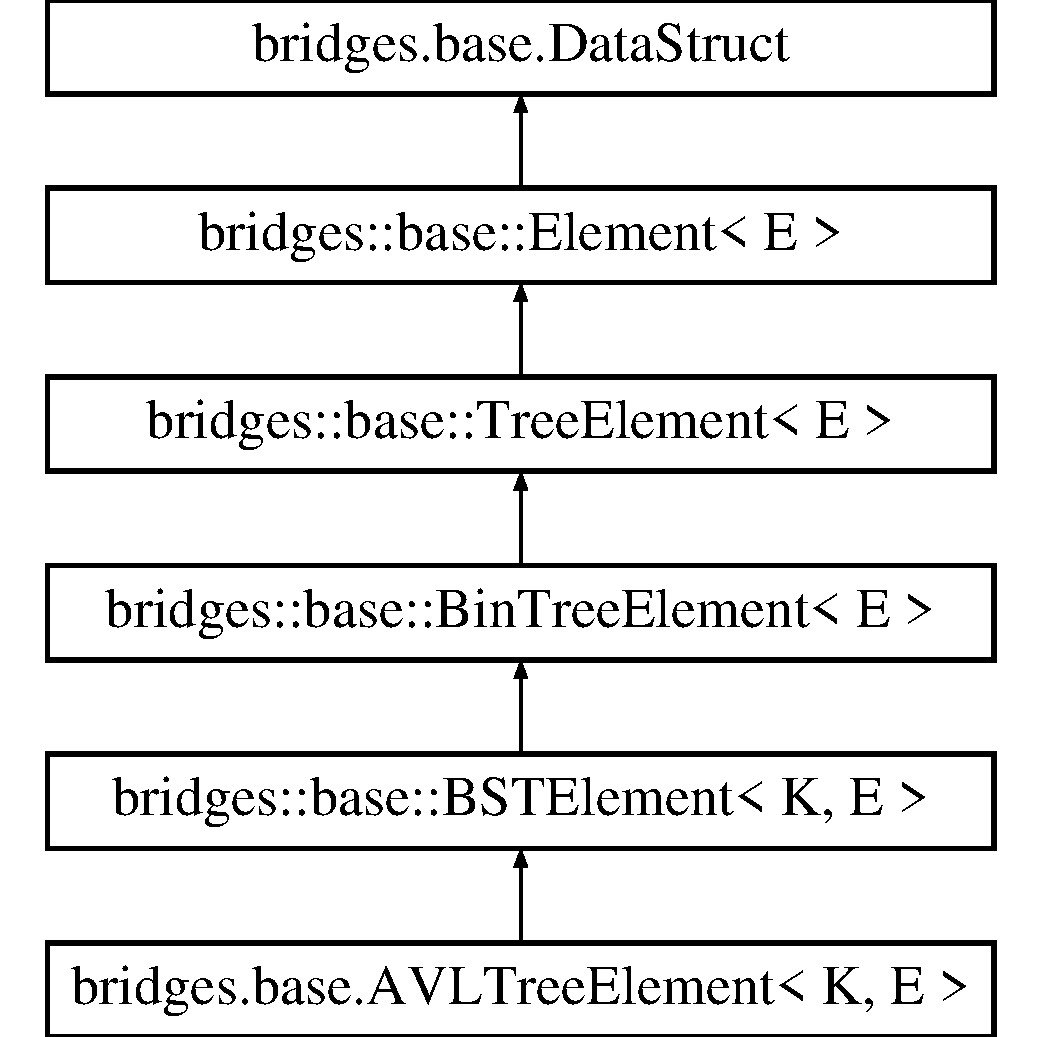
\includegraphics[height=6.000000cm]{classbridges_1_1base_1_1_a_v_l_tree_element}
\end{center}
\end{figure}


\subsection{Detailed Description}
This class extends the \mbox{\hyperlink{classbridges_1_1base_1_1_b_s_t_element}{B\+S\+T\+Element}} class by adding a height and balance factor fields that are useful in A\+VL trees. 

A\+VL tree elements include a \textquotesingle{}height\textquotesingle{} and a \textquotesingle{}bal\+Factor\textquotesingle{} value, representing the height and balance factor of the A\+VL tree at that node, respectively. This is useful in representing A\+VL trees.

A\+V\+L\+Tree elements contain a visualizer (\mbox{\hyperlink{classbridges_1_1base_1_1_element_visualizer}{Element\+Visualizer}}) object for setting visual attributes (color, shape, opacity, size), necessary for displaying them in a web browser.

A\+V\+L\+Tree elements also have a \mbox{\hyperlink{classbridges_1_1base_1_1_link_visualizer}{Link\+Visualizer}} object, that is used when they are linked to another element, appropriate for setting link attributes, for instance, between the current element and its left or right child

\begin{DoxySeeAlso}{See also}
Example tutorial using \mbox{\hyperlink{classbridges_1_1base_1_1_a_v_l_tree_element}{A\+V\+L\+Tree\+Element}} at \href{http://bridgesuncc.github.io/tutorials/AVL.html}{\tt http\+://bridgesuncc.\+github.\+io/tutorials/\+A\+V\+L.\+html}
\end{DoxySeeAlso}

\begin{DoxyParams}{Parameters}
{\em E} & the generic parameter object that is part of this element, representing application specific data. \\
\hline
{\em K} & is the search key parameter in the A\+VL tree node; K must be orderable, such as integer, float, string, etc., on which relational operators work.\\
\hline
\end{DoxyParams}
\begin{DoxyAuthor}{Author}
Kalpathi Subramanian, Mihai Mehedint
\end{DoxyAuthor}
\begin{DoxyDate}{Date}
6/22/16, 1/7/17, 5/17/17, 7/12/19 
\end{DoxyDate}
\subsection*{Public Member Functions}
\begin{DoxyCompactItemize}
\item 
\mbox{\hyperlink{classbridges_1_1base_1_1_a_v_l_tree_element_a8fe4490d3d5d16991736bd1a7243b904}{A\+V\+L\+Tree\+Element}} ()
\item 
\mbox{\hyperlink{classbridges_1_1base_1_1_a_v_l_tree_element_a060ec94b52675313ad15388e3f292df5}{A\+V\+L\+Tree\+Element}} (K k, E e)
\item 
String \mbox{\hyperlink{classbridges_1_1base_1_1_a_v_l_tree_element_abdd9e63de10732ef46bd5d531bd7f9d8}{get\+Data\+Struct\+Type}} ()
\item 
int \mbox{\hyperlink{classbridges_1_1base_1_1_a_v_l_tree_element_a52fe2886334c841547d238db69022697}{get\+Height}} ()
\item 
void \mbox{\hyperlink{classbridges_1_1base_1_1_a_v_l_tree_element_ac42b744989ed7e18dcbd52980e674b33}{set\+Height}} (int h)
\item 
int \mbox{\hyperlink{classbridges_1_1base_1_1_a_v_l_tree_element_a0478ca0351cd714e8f7b8e49703990c8}{get\+Balance\+Factor}} ()
\item 
void \mbox{\hyperlink{classbridges_1_1base_1_1_a_v_l_tree_element_a0dc3c83e750cc39535afb08ea92f6c98}{set\+Balance\+Factor}} (int bf)
\item 
\mbox{\hyperlink{classbridges_1_1base_1_1_a_v_l_tree_element}{A\+V\+L\+Tree\+Element}}$<$ K, E $>$ \mbox{\hyperlink{classbridges_1_1base_1_1_a_v_l_tree_element_a86f1329b19d2886ba7bf713e3844ecd6}{get\+Left}} ()
\item 
\mbox{\hyperlink{classbridges_1_1base_1_1_a_v_l_tree_element}{A\+V\+L\+Tree\+Element}}$<$ K, E $>$ \mbox{\hyperlink{classbridges_1_1base_1_1_a_v_l_tree_element_aab93418ac19605f2c7c57aa38d110921}{get\+Right}} ()
\item 
String \mbox{\hyperlink{classbridges_1_1base_1_1_a_v_l_tree_element_af7ab86f2421864daa4fdc2e84939f4ce}{get\+Element\+Representation}} ()
\end{DoxyCompactItemize}
\subsection*{Additional Inherited Members}


\subsection{Constructor \& Destructor Documentation}
\mbox{\Hypertarget{classbridges_1_1base_1_1_a_v_l_tree_element_a8fe4490d3d5d16991736bd1a7243b904}\label{classbridges_1_1base_1_1_a_v_l_tree_element_a8fe4490d3d5d16991736bd1a7243b904}} 
\index{bridges\+::base\+::\+A\+V\+L\+Tree\+Element@{bridges\+::base\+::\+A\+V\+L\+Tree\+Element}!A\+V\+L\+Tree\+Element@{A\+V\+L\+Tree\+Element}}
\index{A\+V\+L\+Tree\+Element@{A\+V\+L\+Tree\+Element}!bridges\+::base\+::\+A\+V\+L\+Tree\+Element@{bridges\+::base\+::\+A\+V\+L\+Tree\+Element}}
\subsubsection{\texorpdfstring{A\+V\+L\+Tree\+Element()}{AVLTreeElement()}\hspace{0.1cm}{\footnotesize\ttfamily [1/2]}}
{\footnotesize\ttfamily \mbox{\hyperlink{classbridges_1_1base_1_1_a_v_l_tree_element}{bridges.\+base.\+A\+V\+L\+Tree\+Element}}$<$ K, E $>$.\mbox{\hyperlink{classbridges_1_1base_1_1_a_v_l_tree_element}{A\+V\+L\+Tree\+Element}} (\begin{DoxyParamCaption}{ }\end{DoxyParamCaption})}

Construct an \mbox{\hyperlink{classbridges_1_1base_1_1_a_v_l_tree_element}{A\+V\+L\+Tree\+Element}} with default values \mbox{\Hypertarget{classbridges_1_1base_1_1_a_v_l_tree_element_a060ec94b52675313ad15388e3f292df5}\label{classbridges_1_1base_1_1_a_v_l_tree_element_a060ec94b52675313ad15388e3f292df5}} 
\index{bridges\+::base\+::\+A\+V\+L\+Tree\+Element@{bridges\+::base\+::\+A\+V\+L\+Tree\+Element}!A\+V\+L\+Tree\+Element@{A\+V\+L\+Tree\+Element}}
\index{A\+V\+L\+Tree\+Element@{A\+V\+L\+Tree\+Element}!bridges\+::base\+::\+A\+V\+L\+Tree\+Element@{bridges\+::base\+::\+A\+V\+L\+Tree\+Element}}
\subsubsection{\texorpdfstring{A\+V\+L\+Tree\+Element()}{AVLTreeElement()}\hspace{0.1cm}{\footnotesize\ttfamily [2/2]}}
{\footnotesize\ttfamily \mbox{\hyperlink{classbridges_1_1base_1_1_a_v_l_tree_element}{bridges.\+base.\+A\+V\+L\+Tree\+Element}}$<$ K, E $>$.\mbox{\hyperlink{classbridges_1_1base_1_1_a_v_l_tree_element}{A\+V\+L\+Tree\+Element}} (\begin{DoxyParamCaption}\item[{K}]{k,  }\item[{E}]{e }\end{DoxyParamCaption})}

Construct an \mbox{\hyperlink{classbridges_1_1base_1_1_a_v_l_tree_element}{A\+V\+L\+Tree\+Element}} holding a key value \char`\"{}k\char`\"{} and an object \char`\"{}e\char`\"{}


\begin{DoxyParams}{Parameters}
{\em k} & the search key \\
\hline
{\em e} & the appl specific object that \mbox{\hyperlink{classbridges_1_1base_1_1_element}{Element}} is holding \\
\hline
\end{DoxyParams}


\subsection{Member Function Documentation}
\mbox{\Hypertarget{classbridges_1_1base_1_1_a_v_l_tree_element_a0478ca0351cd714e8f7b8e49703990c8}\label{classbridges_1_1base_1_1_a_v_l_tree_element_a0478ca0351cd714e8f7b8e49703990c8}} 
\index{bridges\+::base\+::\+A\+V\+L\+Tree\+Element@{bridges\+::base\+::\+A\+V\+L\+Tree\+Element}!get\+Balance\+Factor@{get\+Balance\+Factor}}
\index{get\+Balance\+Factor@{get\+Balance\+Factor}!bridges\+::base\+::\+A\+V\+L\+Tree\+Element@{bridges\+::base\+::\+A\+V\+L\+Tree\+Element}}
\subsubsection{\texorpdfstring{get\+Balance\+Factor()}{getBalanceFactor()}}
{\footnotesize\ttfamily int \mbox{\hyperlink{classbridges_1_1base_1_1_a_v_l_tree_element}{bridges.\+base.\+A\+V\+L\+Tree\+Element}}$<$ K, E $>$.get\+Balance\+Factor (\begin{DoxyParamCaption}{ }\end{DoxyParamCaption})}

This method returns the balance factor of the tree at this node

\begin{DoxyReturn}{Returns}
balance factor 
\end{DoxyReturn}
\mbox{\Hypertarget{classbridges_1_1base_1_1_a_v_l_tree_element_abdd9e63de10732ef46bd5d531bd7f9d8}\label{classbridges_1_1base_1_1_a_v_l_tree_element_abdd9e63de10732ef46bd5d531bd7f9d8}} 
\index{bridges\+::base\+::\+A\+V\+L\+Tree\+Element@{bridges\+::base\+::\+A\+V\+L\+Tree\+Element}!get\+Data\+Struct\+Type@{get\+Data\+Struct\+Type}}
\index{get\+Data\+Struct\+Type@{get\+Data\+Struct\+Type}!bridges\+::base\+::\+A\+V\+L\+Tree\+Element@{bridges\+::base\+::\+A\+V\+L\+Tree\+Element}}
\subsubsection{\texorpdfstring{get\+Data\+Struct\+Type()}{getDataStructType()}}
{\footnotesize\ttfamily String \mbox{\hyperlink{classbridges_1_1base_1_1_a_v_l_tree_element}{bridges.\+base.\+A\+V\+L\+Tree\+Element}}$<$ K, E $>$.get\+Data\+Struct\+Type (\begin{DoxyParamCaption}{ }\end{DoxyParamCaption})}

This method gets the data structure type

\begin{DoxyReturn}{Returns}
The date structure type as a string 
\end{DoxyReturn}
\mbox{\Hypertarget{classbridges_1_1base_1_1_a_v_l_tree_element_af7ab86f2421864daa4fdc2e84939f4ce}\label{classbridges_1_1base_1_1_a_v_l_tree_element_af7ab86f2421864daa4fdc2e84939f4ce}} 
\index{bridges\+::base\+::\+A\+V\+L\+Tree\+Element@{bridges\+::base\+::\+A\+V\+L\+Tree\+Element}!get\+Element\+Representation@{get\+Element\+Representation}}
\index{get\+Element\+Representation@{get\+Element\+Representation}!bridges\+::base\+::\+A\+V\+L\+Tree\+Element@{bridges\+::base\+::\+A\+V\+L\+Tree\+Element}}
\subsubsection{\texorpdfstring{get\+Element\+Representation()}{getElementRepresentation()}}
{\footnotesize\ttfamily String \mbox{\hyperlink{classbridges_1_1base_1_1_a_v_l_tree_element}{bridges.\+base.\+A\+V\+L\+Tree\+Element}}$<$ K, E $>$.get\+Element\+Representation (\begin{DoxyParamCaption}{ }\end{DoxyParamCaption})}

Augment the element with the \char`\"{}height\char`\"{} and \char`\"{}balance factor\char`\"{} fields.

\begin{DoxyReturn}{Returns}
the augmented J\+S\+ON string 
\end{DoxyReturn}
\mbox{\Hypertarget{classbridges_1_1base_1_1_a_v_l_tree_element_a52fe2886334c841547d238db69022697}\label{classbridges_1_1base_1_1_a_v_l_tree_element_a52fe2886334c841547d238db69022697}} 
\index{bridges\+::base\+::\+A\+V\+L\+Tree\+Element@{bridges\+::base\+::\+A\+V\+L\+Tree\+Element}!get\+Height@{get\+Height}}
\index{get\+Height@{get\+Height}!bridges\+::base\+::\+A\+V\+L\+Tree\+Element@{bridges\+::base\+::\+A\+V\+L\+Tree\+Element}}
\subsubsection{\texorpdfstring{get\+Height()}{getHeight()}}
{\footnotesize\ttfamily int \mbox{\hyperlink{classbridges_1_1base_1_1_a_v_l_tree_element}{bridges.\+base.\+A\+V\+L\+Tree\+Element}}$<$ K, E $>$.get\+Height (\begin{DoxyParamCaption}{ }\end{DoxyParamCaption})}

This method returns the height of the tree at this node

\begin{DoxyReturn}{Returns}
height 
\end{DoxyReturn}
\mbox{\Hypertarget{classbridges_1_1base_1_1_a_v_l_tree_element_a86f1329b19d2886ba7bf713e3844ecd6}\label{classbridges_1_1base_1_1_a_v_l_tree_element_a86f1329b19d2886ba7bf713e3844ecd6}} 
\index{bridges\+::base\+::\+A\+V\+L\+Tree\+Element@{bridges\+::base\+::\+A\+V\+L\+Tree\+Element}!get\+Left@{get\+Left}}
\index{get\+Left@{get\+Left}!bridges\+::base\+::\+A\+V\+L\+Tree\+Element@{bridges\+::base\+::\+A\+V\+L\+Tree\+Element}}
\subsubsection{\texorpdfstring{get\+Left()}{getLeft()}}
{\footnotesize\ttfamily \mbox{\hyperlink{classbridges_1_1base_1_1_a_v_l_tree_element}{A\+V\+L\+Tree\+Element}}$<$K, E$>$ \mbox{\hyperlink{classbridges_1_1base_1_1_a_v_l_tree_element}{bridges.\+base.\+A\+V\+L\+Tree\+Element}}$<$ K, E $>$.get\+Left (\begin{DoxyParamCaption}{ }\end{DoxyParamCaption})}

This method returns the left child of the tree node

\begin{DoxyReturn}{Returns}
the left child of this node 
\end{DoxyReturn}
\mbox{\Hypertarget{classbridges_1_1base_1_1_a_v_l_tree_element_aab93418ac19605f2c7c57aa38d110921}\label{classbridges_1_1base_1_1_a_v_l_tree_element_aab93418ac19605f2c7c57aa38d110921}} 
\index{bridges\+::base\+::\+A\+V\+L\+Tree\+Element@{bridges\+::base\+::\+A\+V\+L\+Tree\+Element}!get\+Right@{get\+Right}}
\index{get\+Right@{get\+Right}!bridges\+::base\+::\+A\+V\+L\+Tree\+Element@{bridges\+::base\+::\+A\+V\+L\+Tree\+Element}}
\subsubsection{\texorpdfstring{get\+Right()}{getRight()}}
{\footnotesize\ttfamily \mbox{\hyperlink{classbridges_1_1base_1_1_a_v_l_tree_element}{A\+V\+L\+Tree\+Element}}$<$K, E$>$ \mbox{\hyperlink{classbridges_1_1base_1_1_a_v_l_tree_element}{bridges.\+base.\+A\+V\+L\+Tree\+Element}}$<$ K, E $>$.get\+Right (\begin{DoxyParamCaption}{ }\end{DoxyParamCaption})}

This method returns the right child of tree node

\begin{DoxyReturn}{Returns}
the right child of this node 
\end{DoxyReturn}
\mbox{\Hypertarget{classbridges_1_1base_1_1_a_v_l_tree_element_a0dc3c83e750cc39535afb08ea92f6c98}\label{classbridges_1_1base_1_1_a_v_l_tree_element_a0dc3c83e750cc39535afb08ea92f6c98}} 
\index{bridges\+::base\+::\+A\+V\+L\+Tree\+Element@{bridges\+::base\+::\+A\+V\+L\+Tree\+Element}!set\+Balance\+Factor@{set\+Balance\+Factor}}
\index{set\+Balance\+Factor@{set\+Balance\+Factor}!bridges\+::base\+::\+A\+V\+L\+Tree\+Element@{bridges\+::base\+::\+A\+V\+L\+Tree\+Element}}
\subsubsection{\texorpdfstring{set\+Balance\+Factor()}{setBalanceFactor()}}
{\footnotesize\ttfamily void \mbox{\hyperlink{classbridges_1_1base_1_1_a_v_l_tree_element}{bridges.\+base.\+A\+V\+L\+Tree\+Element}}$<$ K, E $>$.set\+Balance\+Factor (\begin{DoxyParamCaption}\item[{int}]{bf }\end{DoxyParamCaption})}

This method sets the balance factor of the tree at this node


\begin{DoxyParams}{Parameters}
{\em bf} & balance factor \\
\hline
\end{DoxyParams}
\mbox{\Hypertarget{classbridges_1_1base_1_1_a_v_l_tree_element_ac42b744989ed7e18dcbd52980e674b33}\label{classbridges_1_1base_1_1_a_v_l_tree_element_ac42b744989ed7e18dcbd52980e674b33}} 
\index{bridges\+::base\+::\+A\+V\+L\+Tree\+Element@{bridges\+::base\+::\+A\+V\+L\+Tree\+Element}!set\+Height@{set\+Height}}
\index{set\+Height@{set\+Height}!bridges\+::base\+::\+A\+V\+L\+Tree\+Element@{bridges\+::base\+::\+A\+V\+L\+Tree\+Element}}
\subsubsection{\texorpdfstring{set\+Height()}{setHeight()}}
{\footnotesize\ttfamily void \mbox{\hyperlink{classbridges_1_1base_1_1_a_v_l_tree_element}{bridges.\+base.\+A\+V\+L\+Tree\+Element}}$<$ K, E $>$.set\+Height (\begin{DoxyParamCaption}\item[{int}]{h }\end{DoxyParamCaption})}

This method sets the height of the tree at this node


\begin{DoxyParams}{Parameters}
{\em h} & height \\
\hline
\end{DoxyParams}


The documentation for this class was generated from the following file\+:\begin{DoxyCompactItemize}
\item 
/\+Users/kalpathi/gr/bridges/client/java/src/main/java/bridges/base/\mbox{\hyperlink{_a_v_l_tree_element_8java}{A\+V\+L\+Tree\+Element.\+java}}\end{DoxyCompactItemize}

\hypertarget{classbridges_1_1benchmark_1_1_b_f_s_benchmark}{}\section{bridges\+::benchmark\+::B\+F\+S\+Benchmark Class Reference}
\label{classbridges_1_1benchmark_1_1_b_f_s_benchmark}\index{bridges::benchmark::BFSBenchmark@{bridges::benchmark::BFSBenchmark}}


{\ttfamily \#include $<$B\+F\+S\+Benchmark.\+h$>$}

Inheritance diagram for bridges\+::benchmark\+::B\+F\+S\+Benchmark\+:\begin{figure}[H]
\begin{center}
\leavevmode
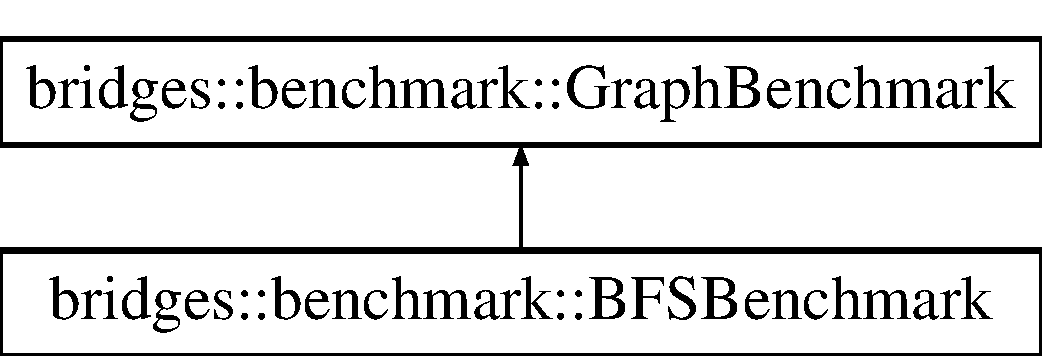
\includegraphics[height=2.000000cm]{classbridges_1_1benchmark_1_1_b_f_s_benchmark}
\end{center}
\end{figure}


\subsection{Detailed Description}
Benchmarks Breadth First Search algorithms. 

Benchmarks B\+FS algorithms and add time series to a Line\+Chart.

One can also set a maximum time spent on a particular run using \mbox{\hyperlink{classbridges_1_1benchmark_1_1_graph_benchmark_a56934eb2789e54c088e7b4423c3a7456}{set\+Time\+Cap()}}.

The B\+FS algorithms must have for prototype\+:

void ($\ast$bfsalgo)(const Graph\+Adj\+List$<$std\+::string$>$\& gr, std\+::string root, std\+::unordered\+\_\+map$<$std\+::string, int$>$\& level, std\+::unordered\+\_\+map$<$std\+::string, std\+::string$>$\& parent);

and can be passed to the run function for being benchmarked. A typical use would look something like


\begin{DoxyCode}{0}
\DoxyCodeLine{LineChart lc;}
\DoxyCodeLine{\mbox{\hyperlink{classbridges_1_1benchmark_1_1_b_f_s_benchmark_abd3525c2c0512a397c29ca41ae6982df}{BFSBenchmark}} sb (lc);}
\DoxyCodeLine{sb.run(\textcolor{stringliteral}{"mybfsalgorithm"}, bfsalgo);}
\end{DoxyCode}


\begin{DoxyAuthor}{Author}
Erik Saule 
\end{DoxyAuthor}
\begin{DoxyDate}{Date}
07/21/2019 
\end{DoxyDate}
\subsection*{Public Member Functions}
\begin{DoxyCompactItemize}
\item 
\mbox{\hyperlink{classbridges_1_1benchmark_1_1_b_f_s_benchmark_abd3525c2c0512a397c29ca41ae6982df}{B\+F\+S\+Benchmark}} (\mbox{\hyperlink{classbridges_1_1datastructure_1_1_line_chart}{Line\+Chart}} \&p)
\item 
void \mbox{\hyperlink{classbridges_1_1benchmark_1_1_b_f_s_benchmark_a8ac66a16c89ecc01b43dc88f9246885c}{run}} (std\+::string algo\+Name, void($\ast$bfsalgo)(const \mbox{\hyperlink{classbridges_1_1datastructure_1_1_graph_adj_list}{Graph\+Adj\+List}}$<$ std\+::string $>$ \&gr, std\+::string root, std\+::unordered\+\_\+map$<$ std\+::string, int $>$ \&level, std\+::unordered\+\_\+map$<$ std\+::string, std\+::string $>$ \&parent))
\begin{DoxyCompactList}\small\item\em benchmark one implementation \end{DoxyCompactList}\end{DoxyCompactItemize}
\subsection*{Additional Inherited Members}


\subsection{Constructor \& Destructor Documentation}
\mbox{\Hypertarget{classbridges_1_1benchmark_1_1_b_f_s_benchmark_abd3525c2c0512a397c29ca41ae6982df}\label{classbridges_1_1benchmark_1_1_b_f_s_benchmark_abd3525c2c0512a397c29ca41ae6982df}} 
\index{bridges::benchmark::BFSBenchmark@{bridges::benchmark::BFSBenchmark}!BFSBenchmark@{BFSBenchmark}}
\index{BFSBenchmark@{BFSBenchmark}!bridges::benchmark::BFSBenchmark@{bridges::benchmark::BFSBenchmark}}
\subsubsection{\texorpdfstring{BFSBenchmark()}{BFSBenchmark()}}
{\footnotesize\ttfamily bridges\+::benchmark\+::\+B\+F\+S\+Benchmark\+::\+B\+F\+S\+Benchmark (\begin{DoxyParamCaption}\item[{\mbox{\hyperlink{classbridges_1_1datastructure_1_1_line_chart}{Line\+Chart}} \&}]{p }\end{DoxyParamCaption})\hspace{0.3cm}{\ttfamily [inline]}}



\subsection{Member Function Documentation}
\mbox{\Hypertarget{classbridges_1_1benchmark_1_1_b_f_s_benchmark_a8ac66a16c89ecc01b43dc88f9246885c}\label{classbridges_1_1benchmark_1_1_b_f_s_benchmark_a8ac66a16c89ecc01b43dc88f9246885c}} 
\index{bridges::benchmark::BFSBenchmark@{bridges::benchmark::BFSBenchmark}!run@{run}}
\index{run@{run}!bridges::benchmark::BFSBenchmark@{bridges::benchmark::BFSBenchmark}}
\subsubsection{\texorpdfstring{run()}{run()}}
{\footnotesize\ttfamily void bridges\+::benchmark\+::\+B\+F\+S\+Benchmark\+::run (\begin{DoxyParamCaption}\item[{std\+::string}]{algo\+Name,  }\item[{void($\ast$)(const \mbox{\hyperlink{classbridges_1_1datastructure_1_1_graph_adj_list}{Graph\+Adj\+List}}$<$ std\+::string $>$ \&gr, std\+::string root, std\+::unordered\+\_\+map$<$ std\+::string, int $>$ \&level, std\+::unordered\+\_\+map$<$ std\+::string, std\+::string $>$ \&parent)}]{bfsalgo }\end{DoxyParamCaption})\hspace{0.3cm}{\ttfamily [inline]}}



benchmark one implementation 


\begin{DoxyParams}{Parameters}
{\em algo\+Name} & screen name of the algorithm to be used in the visualization \\
\hline
{\em bfsalgo} & pointer to the sorting function to benchmark \\
\hline
\end{DoxyParams}


The documentation for this class was generated from the following file\+:\begin{DoxyCompactItemize}
\item 
/\+Users/kalpathi/gr/bridges/cxx/src/\mbox{\hyperlink{_b_f_s_benchmark_8h}{B\+F\+S\+Benchmark.\+h}}\end{DoxyCompactItemize}

\hypertarget{classbridges_1_1benchmark_1_1_b_f_s_params}{}\section{bridges.\+benchmark.\+B\+F\+S\+Params Class Reference}
\label{classbridges_1_1benchmark_1_1_b_f_s_params}\index{bridges.\+benchmark.\+B\+F\+S\+Params@{bridges.\+benchmark.\+B\+F\+S\+Params}}


Inherits bridges.\+benchmark.\+Benchmark\+Params.

\subsection*{Public Attributes}
\begin{DoxyCompactItemize}
\item 
\hyperlink{classbridges_1_1base_1_1_graph_adj_list}{Graph\+Adj\+List}$<$ String, String, String $>$ \hyperlink{classbridges_1_1benchmark_1_1_b_f_s_params_a02dcb89b57adca32f76baae05d443503}{graph}
\item 
String \hyperlink{classbridges_1_1benchmark_1_1_b_f_s_params_afb0381b52b0a8eddb60f420f119e4c99}{root}
\item 
Hash\+Map$<$ String, Integer $>$ \hyperlink{classbridges_1_1benchmark_1_1_b_f_s_params_afb4eff1d30d1f3a25d63d1bf8a4577ad}{level}
\item 
Hash\+Map$<$ String, String $>$ \hyperlink{classbridges_1_1benchmark_1_1_b_f_s_params_a2073895d415e83506c9b538b6d40e101}{parent}
\end{DoxyCompactItemize}


\subsection{Member Data Documentation}
\mbox{\Hypertarget{classbridges_1_1benchmark_1_1_b_f_s_params_a02dcb89b57adca32f76baae05d443503}\label{classbridges_1_1benchmark_1_1_b_f_s_params_a02dcb89b57adca32f76baae05d443503}} 
\index{bridges\+::benchmark\+::\+B\+F\+S\+Params@{bridges\+::benchmark\+::\+B\+F\+S\+Params}!graph@{graph}}
\index{graph@{graph}!bridges\+::benchmark\+::\+B\+F\+S\+Params@{bridges\+::benchmark\+::\+B\+F\+S\+Params}}
\subsubsection{\texorpdfstring{graph}{graph}}
{\footnotesize\ttfamily \hyperlink{classbridges_1_1base_1_1_graph_adj_list}{Graph\+Adj\+List}$<$String, String, String$>$ bridges.\+benchmark.\+B\+F\+S\+Params.\+graph}

\mbox{\Hypertarget{classbridges_1_1benchmark_1_1_b_f_s_params_afb4eff1d30d1f3a25d63d1bf8a4577ad}\label{classbridges_1_1benchmark_1_1_b_f_s_params_afb4eff1d30d1f3a25d63d1bf8a4577ad}} 
\index{bridges\+::benchmark\+::\+B\+F\+S\+Params@{bridges\+::benchmark\+::\+B\+F\+S\+Params}!level@{level}}
\index{level@{level}!bridges\+::benchmark\+::\+B\+F\+S\+Params@{bridges\+::benchmark\+::\+B\+F\+S\+Params}}
\subsubsection{\texorpdfstring{level}{level}}
{\footnotesize\ttfamily Hash\+Map$<$String, Integer$>$ bridges.\+benchmark.\+B\+F\+S\+Params.\+level}

\mbox{\Hypertarget{classbridges_1_1benchmark_1_1_b_f_s_params_a2073895d415e83506c9b538b6d40e101}\label{classbridges_1_1benchmark_1_1_b_f_s_params_a2073895d415e83506c9b538b6d40e101}} 
\index{bridges\+::benchmark\+::\+B\+F\+S\+Params@{bridges\+::benchmark\+::\+B\+F\+S\+Params}!parent@{parent}}
\index{parent@{parent}!bridges\+::benchmark\+::\+B\+F\+S\+Params@{bridges\+::benchmark\+::\+B\+F\+S\+Params}}
\subsubsection{\texorpdfstring{parent}{parent}}
{\footnotesize\ttfamily Hash\+Map$<$String, String$>$ bridges.\+benchmark.\+B\+F\+S\+Params.\+parent}

\mbox{\Hypertarget{classbridges_1_1benchmark_1_1_b_f_s_params_afb0381b52b0a8eddb60f420f119e4c99}\label{classbridges_1_1benchmark_1_1_b_f_s_params_afb0381b52b0a8eddb60f420f119e4c99}} 
\index{bridges\+::benchmark\+::\+B\+F\+S\+Params@{bridges\+::benchmark\+::\+B\+F\+S\+Params}!root@{root}}
\index{root@{root}!bridges\+::benchmark\+::\+B\+F\+S\+Params@{bridges\+::benchmark\+::\+B\+F\+S\+Params}}
\subsubsection{\texorpdfstring{root}{root}}
{\footnotesize\ttfamily String bridges.\+benchmark.\+B\+F\+S\+Params.\+root}



The documentation for this class was generated from the following file\+:\begin{DoxyCompactItemize}
\item 
/home/erik/work/bridges/bridges-\/java/src/main/java/bridges/benchmark/\hyperlink{_b_f_s_params_8java}{B\+F\+S\+Params.\+java}\end{DoxyCompactItemize}

\hypertarget{classbridges_1_1base_1_1_bin_tree_element}{}\section{bridges.\+base.\+Bin\+Tree\+Element$<$ E $>$ Class Template Reference}
\label{classbridges_1_1base_1_1_bin_tree_element}\index{bridges.\+base.\+Bin\+Tree\+Element$<$ E $>$@{bridges.\+base.\+Bin\+Tree\+Element$<$ E $>$}}


This class is extended from the \hyperlink{classbridges_1_1base_1_1_tree_element}{Tree\+Element} class and can be used to create binary tree element objects.  


Inheritance diagram for bridges.\+base.\+Bin\+Tree\+Element$<$ E $>$\+:\begin{figure}[H]
\begin{center}
\leavevmode
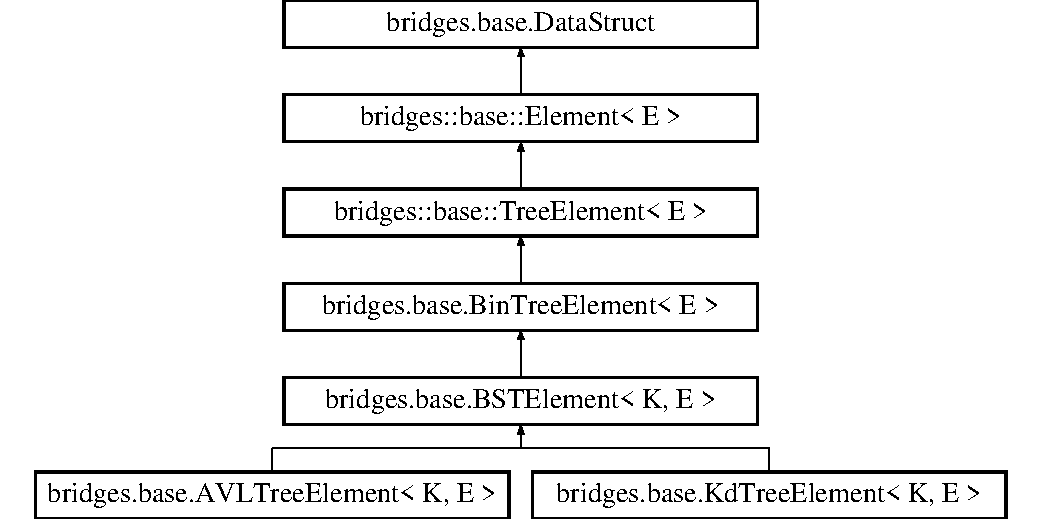
\includegraphics[height=6.000000cm]{classbridges_1_1base_1_1_bin_tree_element}
\end{center}
\end{figure}
\subsection*{Public Member Functions}
\begin{DoxyCompactItemize}
\item 
\hyperlink{classbridges_1_1base_1_1_bin_tree_element_ad6dbf38d53a78be561039c46bde8bc47}{Bin\+Tree\+Element} ()
\item 
\hyperlink{classbridges_1_1base_1_1_bin_tree_element_a2d31fa068f962ced8702fdb4b36c9186}{Bin\+Tree\+Element} (E e)
\item 
\hyperlink{classbridges_1_1base_1_1_bin_tree_element_aac0e300f53d5c1c89b747a1f2c5d54c9}{Bin\+Tree\+Element} (String label, E e)
\item 
\hyperlink{classbridges_1_1base_1_1_bin_tree_element_ab402fac72353087b1b93e82db007e1d7}{Bin\+Tree\+Element} (\hyperlink{classbridges_1_1base_1_1_bin_tree_element}{Bin\+Tree\+Element}$<$ E $>$ left, \hyperlink{classbridges_1_1base_1_1_bin_tree_element}{Bin\+Tree\+Element}$<$ E $>$ right)
\item 
\hyperlink{classbridges_1_1base_1_1_bin_tree_element_a37f3def3cdf4a9eccf577d0ff3c704e9}{Bin\+Tree\+Element} (E e, \hyperlink{classbridges_1_1base_1_1_bin_tree_element}{Bin\+Tree\+Element}$<$ E $>$ left, \hyperlink{classbridges_1_1base_1_1_bin_tree_element}{Bin\+Tree\+Element}$<$ E $>$ right)
\item 
String \hyperlink{classbridges_1_1base_1_1_bin_tree_element_a60fa936692e168f70fb8567090c98883}{get\+Data\+Struct\+Type} ()
\item 
\hyperlink{classbridges_1_1base_1_1_bin_tree_element}{Bin\+Tree\+Element}$<$ E $>$ \hyperlink{classbridges_1_1base_1_1_bin_tree_element_aeb6fd894af8e158c9c48dd0749d1bd22}{get\+Left} ()
\item 
void \hyperlink{classbridges_1_1base_1_1_bin_tree_element_a5bcc2c1374a49f7ab2523ce53d204c30}{set\+Left} (\hyperlink{classbridges_1_1base_1_1_bin_tree_element}{Bin\+Tree\+Element}$<$ E $>$ left)
\item 
\hyperlink{classbridges_1_1base_1_1_bin_tree_element}{Bin\+Tree\+Element}$<$ E $>$ \hyperlink{classbridges_1_1base_1_1_bin_tree_element_aa3855c26617ada7248a9d4f83cf455b7}{get\+Right} ()
\item 
void \hyperlink{classbridges_1_1base_1_1_bin_tree_element_abc40e3ed4cfaf4b74aacfd3657e89ebc}{set\+Right} (\hyperlink{classbridges_1_1base_1_1_bin_tree_element}{Bin\+Tree\+Element}$<$ E $>$ right)
\end{DoxyCompactItemize}
\subsection*{Additional Inherited Members}


\subsection{Detailed Description}
This class is extended from the \hyperlink{classbridges_1_1base_1_1_tree_element}{Tree\+Element} class and can be used to create binary tree element objects. 

The Bin\+Tree element class is the building block for creating binary tree structures. It contains two children (viz., left, right).

\hyperlink{classbridges_1_1base_1_1_bin_tree_element}{Bin\+Tree\+Element} contains a visualizer (\hyperlink{classbridges_1_1base_1_1_element_visualizer}{Element\+Visualizer}) object for setting visual attributes (color, shape, opacity, size), necessary for displaying them in a web browser.

Elements also have a \hyperlink{classbridges_1_1base_1_1_link_visualizer}{Link\+Visualizer} object, that is used when they are linked to another element, appropriate for setting link attributes, for instance, between the current element and its left or right child


\begin{DoxyParams}{Parameters}
{\em E} & he generic parameter object that is part of this element, representing application specific data.\\
\hline
\end{DoxyParams}
\begin{DoxyAuthor}{Author}
Kalpathi Subramanian, Mihai Mehedint
\end{DoxyAuthor}
\begin{DoxyDate}{Date}
6/22/16, 1/7/17, 5/17/17
\end{DoxyDate}
\begin{DoxySeeAlso}{See also}
Example Tutorial at ~\newline
 \href{http://bridgesuncc.github.io/Hello_World_Tutorials/BTree.html}{\tt http\+://bridgesuncc.\+github.\+io/\+Hello\+\_\+\+World\+\_\+\+Tutorials/\+B\+Tree.\+html} 
\end{DoxySeeAlso}


\subsection{Constructor \& Destructor Documentation}
\hypertarget{classbridges_1_1base_1_1_bin_tree_element_ad6dbf38d53a78be561039c46bde8bc47}{}\label{classbridges_1_1base_1_1_bin_tree_element_ad6dbf38d53a78be561039c46bde8bc47} 
\index{bridges\+::base\+::\+Bin\+Tree\+Element@{bridges\+::base\+::\+Bin\+Tree\+Element}!Bin\+Tree\+Element@{Bin\+Tree\+Element}}
\index{Bin\+Tree\+Element@{Bin\+Tree\+Element}!bridges\+::base\+::\+Bin\+Tree\+Element@{bridges\+::base\+::\+Bin\+Tree\+Element}}
\subsubsection{\texorpdfstring{Bin\+Tree\+Element()}{BinTreeElement()}\hspace{0.1cm}{\footnotesize\ttfamily [1/5]}}
{\footnotesize\ttfamily \hyperlink{classbridges_1_1base_1_1_bin_tree_element}{bridges.\+base.\+Bin\+Tree\+Element}$<$ E $>$.\hyperlink{classbridges_1_1base_1_1_bin_tree_element}{Bin\+Tree\+Element} (\begin{DoxyParamCaption}{ }\end{DoxyParamCaption})}

Constructs an empty Binary Tree \hyperlink{classbridges_1_1base_1_1_element}{Element} with right and left pointers set to null. \hypertarget{classbridges_1_1base_1_1_bin_tree_element_a2d31fa068f962ced8702fdb4b36c9186}{}\label{classbridges_1_1base_1_1_bin_tree_element_a2d31fa068f962ced8702fdb4b36c9186} 
\index{bridges\+::base\+::\+Bin\+Tree\+Element@{bridges\+::base\+::\+Bin\+Tree\+Element}!Bin\+Tree\+Element@{Bin\+Tree\+Element}}
\index{Bin\+Tree\+Element@{Bin\+Tree\+Element}!bridges\+::base\+::\+Bin\+Tree\+Element@{bridges\+::base\+::\+Bin\+Tree\+Element}}
\subsubsection{\texorpdfstring{Bin\+Tree\+Element()}{BinTreeElement()}\hspace{0.1cm}{\footnotesize\ttfamily [2/5]}}
{\footnotesize\ttfamily \hyperlink{classbridges_1_1base_1_1_bin_tree_element}{bridges.\+base.\+Bin\+Tree\+Element}$<$ E $>$.\hyperlink{classbridges_1_1base_1_1_bin_tree_element}{Bin\+Tree\+Element} (\begin{DoxyParamCaption}\item[{E}]{e }\end{DoxyParamCaption})}

Constructs a \hyperlink{classbridges_1_1base_1_1_tree_element}{Tree\+Element} holding an object \char`\"{}e\char`\"{} with right and left pointers set to null.


\begin{DoxyParams}{Parameters}
{\em e} & the generic object that \hyperlink{classbridges_1_1base_1_1_tree_element}{Tree\+Element} will hold \\
\hline
\end{DoxyParams}
\hypertarget{classbridges_1_1base_1_1_bin_tree_element_aac0e300f53d5c1c89b747a1f2c5d54c9}{}\label{classbridges_1_1base_1_1_bin_tree_element_aac0e300f53d5c1c89b747a1f2c5d54c9} 
\index{bridges\+::base\+::\+Bin\+Tree\+Element@{bridges\+::base\+::\+Bin\+Tree\+Element}!Bin\+Tree\+Element@{Bin\+Tree\+Element}}
\index{Bin\+Tree\+Element@{Bin\+Tree\+Element}!bridges\+::base\+::\+Bin\+Tree\+Element@{bridges\+::base\+::\+Bin\+Tree\+Element}}
\subsubsection{\texorpdfstring{Bin\+Tree\+Element()}{BinTreeElement()}\hspace{0.1cm}{\footnotesize\ttfamily [3/5]}}
{\footnotesize\ttfamily \hyperlink{classbridges_1_1base_1_1_bin_tree_element}{bridges.\+base.\+Bin\+Tree\+Element}$<$ E $>$.\hyperlink{classbridges_1_1base_1_1_bin_tree_element}{Bin\+Tree\+Element} (\begin{DoxyParamCaption}\item[{String}]{label,  }\item[{E}]{e }\end{DoxyParamCaption})}

Constructs a \hyperlink{classbridges_1_1base_1_1_tree_element}{Tree\+Element} with label set to \char`\"{}label\char`\"{}, holding an object \char`\"{}e\char`\"{}.


\begin{DoxyParams}{Parameters}
{\em label} & the label of \hyperlink{classbridges_1_1base_1_1_tree_element}{Tree\+Element} that shows up on the Bridges visualization\\
\hline
{\em e} & the generic object that \hyperlink{classbridges_1_1base_1_1_tree_element}{Tree\+Element} will hold \\
\hline
\end{DoxyParams}
\hypertarget{classbridges_1_1base_1_1_bin_tree_element_ab402fac72353087b1b93e82db007e1d7}{}\label{classbridges_1_1base_1_1_bin_tree_element_ab402fac72353087b1b93e82db007e1d7} 
\index{bridges\+::base\+::\+Bin\+Tree\+Element@{bridges\+::base\+::\+Bin\+Tree\+Element}!Bin\+Tree\+Element@{Bin\+Tree\+Element}}
\index{Bin\+Tree\+Element@{Bin\+Tree\+Element}!bridges\+::base\+::\+Bin\+Tree\+Element@{bridges\+::base\+::\+Bin\+Tree\+Element}}
\subsubsection{\texorpdfstring{Bin\+Tree\+Element()}{BinTreeElement()}\hspace{0.1cm}{\footnotesize\ttfamily [4/5]}}
{\footnotesize\ttfamily \hyperlink{classbridges_1_1base_1_1_bin_tree_element}{bridges.\+base.\+Bin\+Tree\+Element}$<$ E $>$.\hyperlink{classbridges_1_1base_1_1_bin_tree_element}{Bin\+Tree\+Element} (\begin{DoxyParamCaption}\item[{\hyperlink{classbridges_1_1base_1_1_bin_tree_element}{Bin\+Tree\+Element}$<$ E $>$}]{left,  }\item[{\hyperlink{classbridges_1_1base_1_1_bin_tree_element}{Bin\+Tree\+Element}$<$ E $>$}]{right }\end{DoxyParamCaption})}

Constructs an empty \hyperlink{classbridges_1_1base_1_1_tree_element}{Tree\+Element} left pointer pointing to \char`\"{}left\char`\"{} and right pointer pointing to \char`\"{}right\char`\"{}.


\begin{DoxyParams}{Parameters}
{\em left} & the \hyperlink{classbridges_1_1base_1_1_tree_element}{Tree\+Element} to be assigned to the left pointer of this \hyperlink{classbridges_1_1base_1_1_tree_element}{Tree\+Element} \\
\hline
{\em right} & the \hyperlink{classbridges_1_1base_1_1_tree_element}{Tree\+Element} to be assigned to the right pointer of this \hyperlink{classbridges_1_1base_1_1_tree_element}{Tree\+Element} \\
\hline
\end{DoxyParams}
\hypertarget{classbridges_1_1base_1_1_bin_tree_element_a37f3def3cdf4a9eccf577d0ff3c704e9}{}\label{classbridges_1_1base_1_1_bin_tree_element_a37f3def3cdf4a9eccf577d0ff3c704e9} 
\index{bridges\+::base\+::\+Bin\+Tree\+Element@{bridges\+::base\+::\+Bin\+Tree\+Element}!Bin\+Tree\+Element@{Bin\+Tree\+Element}}
\index{Bin\+Tree\+Element@{Bin\+Tree\+Element}!bridges\+::base\+::\+Bin\+Tree\+Element@{bridges\+::base\+::\+Bin\+Tree\+Element}}
\subsubsection{\texorpdfstring{Bin\+Tree\+Element()}{BinTreeElement()}\hspace{0.1cm}{\footnotesize\ttfamily [5/5]}}
{\footnotesize\ttfamily \hyperlink{classbridges_1_1base_1_1_bin_tree_element}{bridges.\+base.\+Bin\+Tree\+Element}$<$ E $>$.\hyperlink{classbridges_1_1base_1_1_bin_tree_element}{Bin\+Tree\+Element} (\begin{DoxyParamCaption}\item[{E}]{e,  }\item[{\hyperlink{classbridges_1_1base_1_1_bin_tree_element}{Bin\+Tree\+Element}$<$ E $>$}]{left,  }\item[{\hyperlink{classbridges_1_1base_1_1_bin_tree_element}{Bin\+Tree\+Element}$<$ E $>$}]{right }\end{DoxyParamCaption})}

Constructs a \hyperlink{classbridges_1_1base_1_1_tree_element}{Tree\+Element} holding the object \char`\"{}e\char`\"{}, left pointer pointing to \char`\"{}left\char`\"{} and right pointer pointing to \char`\"{}right\char`\"{}.


\begin{DoxyParams}{Parameters}
{\em e} & the generic object that \hyperlink{classbridges_1_1base_1_1_tree_element}{Tree\+Element} will hold \\
\hline
{\em left} & the \hyperlink{classbridges_1_1base_1_1_tree_element}{Tree\+Element} to be assigned to the left pointer of this \hyperlink{classbridges_1_1base_1_1_tree_element}{Tree\+Element} \\
\hline
{\em right} & the \hyperlink{classbridges_1_1base_1_1_tree_element}{Tree\+Element} to be assigned to the right pointer of this \hyperlink{classbridges_1_1base_1_1_tree_element}{Tree\+Element} \\
\hline
\end{DoxyParams}


\subsection{Member Function Documentation}
\hypertarget{classbridges_1_1base_1_1_bin_tree_element_a60fa936692e168f70fb8567090c98883}{}\label{classbridges_1_1base_1_1_bin_tree_element_a60fa936692e168f70fb8567090c98883} 
\index{bridges\+::base\+::\+Bin\+Tree\+Element@{bridges\+::base\+::\+Bin\+Tree\+Element}!get\+Data\+Struct\+Type@{get\+Data\+Struct\+Type}}
\index{get\+Data\+Struct\+Type@{get\+Data\+Struct\+Type}!bridges\+::base\+::\+Bin\+Tree\+Element@{bridges\+::base\+::\+Bin\+Tree\+Element}}
\subsubsection{\texorpdfstring{get\+Data\+Struct\+Type()}{getDataStructType()}}
{\footnotesize\ttfamily String \hyperlink{classbridges_1_1base_1_1_bin_tree_element}{bridges.\+base.\+Bin\+Tree\+Element}$<$ E $>$.get\+Data\+Struct\+Type (\begin{DoxyParamCaption}{ }\end{DoxyParamCaption})}

This method gets the data structure type

\begin{DoxyReturn}{Returns}
The date structure type as a string 
\end{DoxyReturn}
\hypertarget{classbridges_1_1base_1_1_bin_tree_element_aeb6fd894af8e158c9c48dd0749d1bd22}{}\label{classbridges_1_1base_1_1_bin_tree_element_aeb6fd894af8e158c9c48dd0749d1bd22} 
\index{bridges\+::base\+::\+Bin\+Tree\+Element@{bridges\+::base\+::\+Bin\+Tree\+Element}!get\+Left@{get\+Left}}
\index{get\+Left@{get\+Left}!bridges\+::base\+::\+Bin\+Tree\+Element@{bridges\+::base\+::\+Bin\+Tree\+Element}}
\subsubsection{\texorpdfstring{get\+Left()}{getLeft()}}
{\footnotesize\ttfamily \hyperlink{classbridges_1_1base_1_1_bin_tree_element}{Bin\+Tree\+Element}$<$E$>$ \hyperlink{classbridges_1_1base_1_1_bin_tree_element}{bridges.\+base.\+Bin\+Tree\+Element}$<$ E $>$.get\+Left (\begin{DoxyParamCaption}{ }\end{DoxyParamCaption})}

This method returns the left tree element pointer \begin{DoxyReturn}{Returns}
the left child of this \hyperlink{classbridges_1_1base_1_1_tree_element}{Tree\+Element} 
\end{DoxyReturn}
\hypertarget{classbridges_1_1base_1_1_bin_tree_element_aa3855c26617ada7248a9d4f83cf455b7}{}\label{classbridges_1_1base_1_1_bin_tree_element_aa3855c26617ada7248a9d4f83cf455b7} 
\index{bridges\+::base\+::\+Bin\+Tree\+Element@{bridges\+::base\+::\+Bin\+Tree\+Element}!get\+Right@{get\+Right}}
\index{get\+Right@{get\+Right}!bridges\+::base\+::\+Bin\+Tree\+Element@{bridges\+::base\+::\+Bin\+Tree\+Element}}
\subsubsection{\texorpdfstring{get\+Right()}{getRight()}}
{\footnotesize\ttfamily \hyperlink{classbridges_1_1base_1_1_bin_tree_element}{Bin\+Tree\+Element}$<$E$>$ \hyperlink{classbridges_1_1base_1_1_bin_tree_element}{bridges.\+base.\+Bin\+Tree\+Element}$<$ E $>$.get\+Right (\begin{DoxyParamCaption}{ }\end{DoxyParamCaption})}

This method returns the right tree element pointer

\begin{DoxyReturn}{Returns}
the right child of this \hyperlink{classbridges_1_1base_1_1_tree_element}{Tree\+Element} 
\end{DoxyReturn}
\hypertarget{classbridges_1_1base_1_1_bin_tree_element_a5bcc2c1374a49f7ab2523ce53d204c30}{}\label{classbridges_1_1base_1_1_bin_tree_element_a5bcc2c1374a49f7ab2523ce53d204c30} 
\index{bridges\+::base\+::\+Bin\+Tree\+Element@{bridges\+::base\+::\+Bin\+Tree\+Element}!set\+Left@{set\+Left}}
\index{set\+Left@{set\+Left}!bridges\+::base\+::\+Bin\+Tree\+Element@{bridges\+::base\+::\+Bin\+Tree\+Element}}
\subsubsection{\texorpdfstring{set\+Left()}{setLeft()}}
{\footnotesize\ttfamily void \hyperlink{classbridges_1_1base_1_1_bin_tree_element}{bridges.\+base.\+Bin\+Tree\+Element}$<$ E $>$.set\+Left (\begin{DoxyParamCaption}\item[{\hyperlink{classbridges_1_1base_1_1_bin_tree_element}{Bin\+Tree\+Element}$<$ E $>$}]{left }\end{DoxyParamCaption})}

This method sets the left tree element pointer 
\begin{DoxyParams}{Parameters}
{\em left} & the \hyperlink{classbridges_1_1base_1_1_tree_element}{Tree\+Element} that should be assigned to the left child \\
\hline
\end{DoxyParams}
\hypertarget{classbridges_1_1base_1_1_bin_tree_element_abc40e3ed4cfaf4b74aacfd3657e89ebc}{}\label{classbridges_1_1base_1_1_bin_tree_element_abc40e3ed4cfaf4b74aacfd3657e89ebc} 
\index{bridges\+::base\+::\+Bin\+Tree\+Element@{bridges\+::base\+::\+Bin\+Tree\+Element}!set\+Right@{set\+Right}}
\index{set\+Right@{set\+Right}!bridges\+::base\+::\+Bin\+Tree\+Element@{bridges\+::base\+::\+Bin\+Tree\+Element}}
\subsubsection{\texorpdfstring{set\+Right()}{setRight()}}
{\footnotesize\ttfamily void \hyperlink{classbridges_1_1base_1_1_bin_tree_element}{bridges.\+base.\+Bin\+Tree\+Element}$<$ E $>$.set\+Right (\begin{DoxyParamCaption}\item[{\hyperlink{classbridges_1_1base_1_1_bin_tree_element}{Bin\+Tree\+Element}$<$ E $>$}]{right }\end{DoxyParamCaption})}

This method sets the right tree element pointer


\begin{DoxyParams}{Parameters}
{\em right} & the \hyperlink{classbridges_1_1base_1_1_tree_element}{Tree\+Element} that should be assigned to the right child \\
\hline
\end{DoxyParams}


The documentation for this class was generated from the following file\+:\begin{DoxyCompactItemize}
\item 
link/base/\hyperlink{_bin_tree_element_8java}{Bin\+Tree\+Element.\+java}\end{DoxyCompactItemize}

\hypertarget{classbridges_1_1games_1_1_blocking_game}{}\doxysection{bridges.\+games.\+Blocking\+Game Class Reference}
\label{classbridges_1_1games_1_1_blocking_game}\index{bridges.games.BlockingGame@{bridges.games.BlockingGame}}
Inheritance diagram for bridges.\+games.\+Blocking\+Game\+:\begin{figure}[H]
\begin{center}
\leavevmode
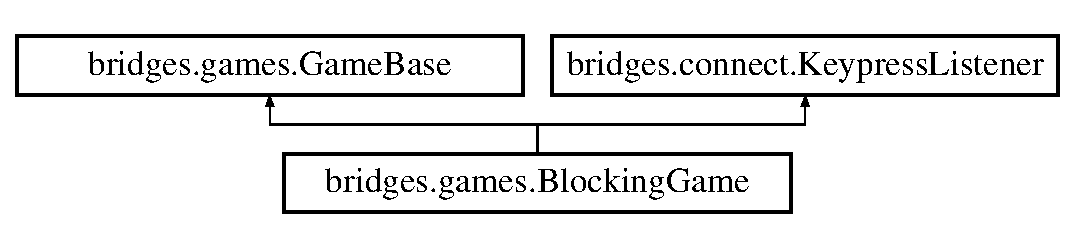
\includegraphics[height=2.000000cm]{classbridges_1_1games_1_1_blocking_game}
\end{center}
\end{figure}
\doxysubsection*{Public Member Functions}
\begin{DoxyCompactItemize}
\item 
void \mbox{\hyperlink{classbridges_1_1games_1_1_blocking_game_a53b1b38826785ee7c7a13f486b7b72ba}{keypress}} (J\+S\+O\+N\+Object keypress)
\item 
String \mbox{\hyperlink{classbridges_1_1games_1_1_blocking_game_ac96929a7b516825835d9c9314ed0fdc1}{get\+Key\+Press}} ()
\item 
\mbox{\hyperlink{classbridges_1_1games_1_1_blocking_game_a0ebcf0a4ae8d81173a58d4458a9538cc}{Blocking\+Game}} (int assid, String login, String apikey, int cols, int rows)
\item 
void \mbox{\hyperlink{classbridges_1_1games_1_1_blocking_game_a00f9ad93393ba18407940f24aaddfa21}{start}} ()
\begin{DoxyCompactList}\small\item\em Call this function from main to start the game. \end{DoxyCompactList}\end{DoxyCompactItemize}
\doxysubsection*{Protected Attributes}
\begin{DoxyCompactItemize}
\item 
Queue$<$ String $>$ \mbox{\hyperlink{classbridges_1_1games_1_1_blocking_game_a7a8057fd0e008879f89c86d929cc92e6}{keyqueue}}
\end{DoxyCompactItemize}
\doxysubsection*{Additional Inherited Members}


\doxysubsection{Constructor \& Destructor Documentation}
\mbox{\Hypertarget{classbridges_1_1games_1_1_blocking_game_a0ebcf0a4ae8d81173a58d4458a9538cc}\label{classbridges_1_1games_1_1_blocking_game_a0ebcf0a4ae8d81173a58d4458a9538cc}} 
\index{bridges.games.BlockingGame@{bridges.games.BlockingGame}!BlockingGame@{BlockingGame}}
\index{BlockingGame@{BlockingGame}!bridges.games.BlockingGame@{bridges.games.BlockingGame}}
\doxysubsubsection{\texorpdfstring{BlockingGame()}{BlockingGame()}}
{\footnotesize\ttfamily bridges.\+games.\+Blocking\+Game.\+Blocking\+Game (\begin{DoxyParamCaption}\item[{int}]{assid,  }\item[{String}]{login,  }\item[{String}]{apikey,  }\item[{int}]{cols,  }\item[{int}]{rows }\end{DoxyParamCaption})}



\doxysubsection{Member Function Documentation}
\mbox{\Hypertarget{classbridges_1_1games_1_1_blocking_game_ac96929a7b516825835d9c9314ed0fdc1}\label{classbridges_1_1games_1_1_blocking_game_ac96929a7b516825835d9c9314ed0fdc1}} 
\index{bridges.games.BlockingGame@{bridges.games.BlockingGame}!getKeyPress@{getKeyPress}}
\index{getKeyPress@{getKeyPress}!bridges.games.BlockingGame@{bridges.games.BlockingGame}}
\doxysubsubsection{\texorpdfstring{getKeyPress()}{getKeyPress()}}
{\footnotesize\ttfamily String bridges.\+games.\+Blocking\+Game.\+get\+Key\+Press (\begin{DoxyParamCaption}{ }\end{DoxyParamCaption})}

\mbox{\Hypertarget{classbridges_1_1games_1_1_blocking_game_a53b1b38826785ee7c7a13f486b7b72ba}\label{classbridges_1_1games_1_1_blocking_game_a53b1b38826785ee7c7a13f486b7b72ba}} 
\index{bridges.games.BlockingGame@{bridges.games.BlockingGame}!keypress@{keypress}}
\index{keypress@{keypress}!bridges.games.BlockingGame@{bridges.games.BlockingGame}}
\doxysubsubsection{\texorpdfstring{keypress()}{keypress()}}
{\footnotesize\ttfamily void bridges.\+games.\+Blocking\+Game.\+keypress (\begin{DoxyParamCaption}\item[{J\+S\+O\+N\+Object}]{keypress }\end{DoxyParamCaption})}



Implements \mbox{\hyperlink{interfacebridges_1_1connect_1_1_keypress_listener_af713d94f36bce842f39ce0aea4db8da6}{bridges.\+connect.\+Keypress\+Listener}}.

\mbox{\Hypertarget{classbridges_1_1games_1_1_blocking_game_a00f9ad93393ba18407940f24aaddfa21}\label{classbridges_1_1games_1_1_blocking_game_a00f9ad93393ba18407940f24aaddfa21}} 
\index{bridges.games.BlockingGame@{bridges.games.BlockingGame}!start@{start}}
\index{start@{start}!bridges.games.BlockingGame@{bridges.games.BlockingGame}}
\doxysubsubsection{\texorpdfstring{start()}{start()}}
{\footnotesize\ttfamily void bridges.\+games.\+Blocking\+Game.\+start (\begin{DoxyParamCaption}{ }\end{DoxyParamCaption})}



Call this function from main to start the game. 



Reimplemented from \mbox{\hyperlink{classbridges_1_1games_1_1_game_base_a4b09bc799726e4a59b1ab039b941b188}{bridges.\+games.\+Game\+Base}}.



\doxysubsection{Member Data Documentation}
\mbox{\Hypertarget{classbridges_1_1games_1_1_blocking_game_a7a8057fd0e008879f89c86d929cc92e6}\label{classbridges_1_1games_1_1_blocking_game_a7a8057fd0e008879f89c86d929cc92e6}} 
\index{bridges.games.BlockingGame@{bridges.games.BlockingGame}!keyqueue@{keyqueue}}
\index{keyqueue@{keyqueue}!bridges.games.BlockingGame@{bridges.games.BlockingGame}}
\doxysubsubsection{\texorpdfstring{keyqueue}{keyqueue}}
{\footnotesize\ttfamily Queue$<$String$>$ bridges.\+games.\+Blocking\+Game.\+keyqueue\hspace{0.3cm}{\ttfamily [protected]}}



The documentation for this class was generated from the following file\+:\begin{DoxyCompactItemize}
\item 
/\+Users/kalpathi/gr/bridges/client/java/src/main/java/bridges/games/\mbox{\hyperlink{_blocking_game_8java}{Blocking\+Game.\+java}}\end{DoxyCompactItemize}

\hypertarget{classbridges_1_1connect_1_1_bridges}{}\section{bridges.\+connect.\+Bridges Class Reference}
\label{classbridges_1_1connect_1_1_bridges}\index{bridges.\+connect.\+Bridges@{bridges.\+connect.\+Bridges}}


\subsection{Detailed Description}
The \hyperlink{classbridges_1_1connect_1_1_bridges}{Bridges} class is the main class that provides interfaces to datasets, maintains user and assignment information, and connects to the \hyperlink{classbridges_1_1connect_1_1_bridges}{Bridges} server. 

The \hyperlink{classbridges_1_1connect_1_1_bridges}{Bridges} class is responsible for initializing the \hyperlink{classbridges_1_1connect_1_1_bridges}{Bridges} system, specifying parameters (user id, assignment id, title, description, data structure type, etc) for the student assignment, generating the data structure representation and transmission to the \hyperlink{classbridges_1_1connect_1_1_bridges}{Bridges} server. In addition, it provides interfaces to a number of real-\/world datasets, that makes it easy to access the data for use algorithms/data structure assignments. ~\newline


{\bfseries Datasets.} The datasets that are currently supported through the B\+R\+I\+D\+G\+ES A\+PI include U\+S\+GS Earthquake Data, I\+M\+DB Actor/\+Movie Data (2 versions), Gutenberg Book Collection Meta Data, a Video Game Dataset and Shakespeare Dataset. More information is found in the respective methods (below) and at 

\href{http://bridgesuncc.github.io/datasets.html}{\tt http\+://bridgesuncc.\+github.\+io/datasets.\+html} 

A typical \hyperlink{classbridges_1_1connect_1_1_bridges}{Bridges} program includes creating the \hyperlink{classbridges_1_1connect_1_1_bridges}{Bridges} object, followed by creation of the data structure by the user, assigning visual attributes to elements of the data structure, followed by specification of teh data structure type and the call to visualize the data structure (\hyperlink{classbridges_1_1connect_1_1_bridges_a921a6603b2445b1abe30a1b3d6f0c255}{Bridges\+::set\+Data\+Structure()} and \hyperlink{classbridges_1_1connect_1_1_bridges_a1853d64ffb8675ba2ec227a2b819cd24}{visualize()} methods).

\begin{DoxyAuthor}{Author}
Sean Gallagher, Kalpathi Subramanaian, Mihai Mehedint, David Burlinson.
\end{DoxyAuthor}
\begin{DoxyDate}{Date}
1/16/17, 5/19/17
\end{DoxyDate}
\begin{DoxySeeAlso}{See also}
Tutorial examples at ~\newline
 \href{http://bridgesuncc.github.io/Hello_World_Tutorials/Overview.html}{\tt http\+://bridgesuncc.\+github.\+io/\+Hello\+\_\+\+World\+\_\+\+Tutorials/\+Overview.\+html} 
\end{DoxySeeAlso}
\subsection*{Public Member Functions}
\begin{DoxyCompactItemize}
\item 
\hyperlink{classbridges_1_1connect_1_1_bridges_a42f0592841a829f93453506c78951b1f}{Bridges} ()
\item 
\hyperlink{classbridges_1_1connect_1_1_data_source}{Data\+Source} \hyperlink{classbridges_1_1connect_1_1_bridges_acfe00a832969a77504d9d33d783c4fcd}{get\+Data\+Source} ()
\item 
\hyperlink{classbridges_1_1connect_1_1_bridges_a4c47eb7cbb94c5810dc38c38760db872}{Bridges} (int assignment, String username, String appl\+\_\+id)
\item 
void \hyperlink{classbridges_1_1connect_1_1_bridges_a87aa73367a43cfc8b3ae5e4926ea4895}{init} (int assignment, String username, String appl\+\_\+id)
\item 
void \hyperlink{classbridges_1_1connect_1_1_bridges_aed3752ee6318a48dff271d9a9e2a8fcc}{set\+Title} (String title)
\begin{DoxyCompactList}\small\item\em Change the title of the assignment. \end{DoxyCompactList}\item 
void \hyperlink{classbridges_1_1connect_1_1_bridges_a50d1d5aa64d312393b63d1be854e34a2}{set\+Description} (String description)
\begin{DoxyCompactList}\small\item\em Change the textual description of the assignment. \end{DoxyCompactList}\item 
void \hyperlink{classbridges_1_1connect_1_1_bridges_ab43e412448e1dfc340e58c407519a576}{set\+Server} (String server)
\item 
void \hyperlink{classbridges_1_1connect_1_1_bridges_a4af383ba2f114ad7bd4e08eb44096973}{set\+Map\+Overlay} (Boolean flag)
\item 
void \hyperlink{classbridges_1_1connect_1_1_bridges_aaa1a44a689daa26a841d0e8d31839861}{set\+Display\+Mode} (String mode)  throws Illegal\+Argument\+Exception 
\item 
void \hyperlink{classbridges_1_1connect_1_1_bridges_ade4a9c43e2b608e6b3dc774b73f95749}{set\+Coord\+System\+Type} (String coord)
\item 
void \hyperlink{classbridges_1_1connect_1_1_bridges_ac2f9a8d7852e499a7ed3521f06d470bf}{set\+Window} (int x1, int x2, int y1, int y2)
\begin{DoxyCompactList}\small\item\em Specify the window that will be used to render the view by default. \end{DoxyCompactList}\item 
void \hyperlink{classbridges_1_1connect_1_1_bridges_afff6882285f7615b775c59b2fc62b1c3}{set\+Window} (float x1, float x2, float y1, float y2)
\begin{DoxyCompactList}\small\item\em Specify the window that will be used to render the view by default. \end{DoxyCompactList}\item 
void \hyperlink{classbridges_1_1connect_1_1_bridges_a163a32a2fd3327c59d003f457e31eb63}{set\+Window} (double x1, double x2, double y1, double y2)
\begin{DoxyCompactList}\small\item\em Specify the window that will be used to render the view by default. \end{DoxyCompactList}\item 
boolean \hyperlink{classbridges_1_1connect_1_1_bridges_afd3c63780396e92c94c923037385b31d}{visualize\+J\+S\+ON} ()
\item 
void \hyperlink{classbridges_1_1connect_1_1_bridges_aa502aa32a9ac482da9c8455c6810b64d}{set\+Visualize\+J\+S\+ON} (boolean flag)
\item 
void \hyperlink{classbridges_1_1connect_1_1_bridges_a921a6603b2445b1abe30a1b3d6f0c255}{set\+Data\+Structure} (\hyperlink{classbridges_1_1base_1_1_data_struct}{Data\+Struct} ds)  throws Null\+Pointer\+Exception 
\item 
void \hyperlink{classbridges_1_1connect_1_1_bridges_ad79081ca241e5bcb77b1ed52a09fdd39}{clear\+Assignment} ()
\item 
void \hyperlink{classbridges_1_1connect_1_1_bridges_a1853d64ffb8675ba2ec227a2b819cd24}{visualize} ()  throws I\+O\+Exception, Rate\+Limit\+Exception 
\end{DoxyCompactItemize}
\subsection*{Static Public Member Functions}
\begin{DoxyCompactItemize}
\item 
static void \hyperlink{classbridges_1_1connect_1_1_bridges_a9295b15aa880aa976706ed4f3337fb3b}{set\+Debug\+Flag} (Boolean flag)
\item 
static Boolean \hyperlink{classbridges_1_1connect_1_1_bridges_a5c9fa0dd62084bfd916c8bdecee3f517}{get\+Debug\+Flag} ()
\item 
static String \hyperlink{classbridges_1_1connect_1_1_bridges_af049c06c532987eb616156fb16ea2f43}{get\+Assignment} ()
\item 
static int \hyperlink{classbridges_1_1connect_1_1_bridges_ac13ed456687540b57c138adb11735d95}{get\+Assignment\+ID} ()
\item 
static void \hyperlink{classbridges_1_1connect_1_1_bridges_ad56c9d138965c41947bb51fe056c1cc9}{set\+Assignment} (int assignment)
\item 
static String \hyperlink{classbridges_1_1connect_1_1_bridges_a75f047cda3100e0cfa88378293c12961}{get\+User\+Name} ()
\item 
static void \hyperlink{classbridges_1_1connect_1_1_bridges_af9b9a2ca03ba02c0c2be4716594678a6}{set\+User\+Name} (String user\+Name)
\item 
static String \hyperlink{classbridges_1_1connect_1_1_bridges_a426897d6e5449601bb4e20c32b8346f5}{get\+Key} ()
\item 
static void \hyperlink{classbridges_1_1connect_1_1_bridges_ab69e89ec7d2e674a8b8c4b0be0c63397}{set\+Key} (String key)
\end{DoxyCompactItemize}


\subsection{Constructor \& Destructor Documentation}
\mbox{\Hypertarget{classbridges_1_1connect_1_1_bridges_a42f0592841a829f93453506c78951b1f}\label{classbridges_1_1connect_1_1_bridges_a42f0592841a829f93453506c78951b1f}} 
\index{bridges\+::connect\+::\+Bridges@{bridges\+::connect\+::\+Bridges}!Bridges@{Bridges}}
\index{Bridges@{Bridges}!bridges\+::connect\+::\+Bridges@{bridges\+::connect\+::\+Bridges}}
\subsubsection{\texorpdfstring{Bridges()}{Bridges()}\hspace{0.1cm}{\footnotesize\ttfamily [1/2]}}
{\footnotesize\ttfamily bridges.\+connect.\+Bridges.\+Bridges (\begin{DoxyParamCaption}{ }\end{DoxyParamCaption})}

Constructors

If the F\+O\+R\+C\+E\+\_\+\+B\+R\+I\+D\+G\+E\+S\+\_\+\+A\+P\+I\+K\+EY environment variable is set, use the environment variable as A\+P\+Ikey in all cases.

If the F\+O\+R\+C\+E\+\_\+\+B\+R\+I\+D\+G\+E\+S\+\_\+\+U\+S\+E\+R\+N\+A\+ME environment variable is set, use the environment variable as username in all cases.

If the F\+O\+R\+C\+E\+\_\+\+B\+R\+I\+D\+G\+E\+S\+\_\+\+A\+S\+S\+I\+G\+N\+M\+E\+NT environment variable is set, use the environment variable as assignment number in all cases. \mbox{\Hypertarget{classbridges_1_1connect_1_1_bridges_a4c47eb7cbb94c5810dc38c38760db872}\label{classbridges_1_1connect_1_1_bridges_a4c47eb7cbb94c5810dc38c38760db872}} 
\index{bridges\+::connect\+::\+Bridges@{bridges\+::connect\+::\+Bridges}!Bridges@{Bridges}}
\index{Bridges@{Bridges}!bridges\+::connect\+::\+Bridges@{bridges\+::connect\+::\+Bridges}}
\subsubsection{\texorpdfstring{Bridges()}{Bridges()}\hspace{0.1cm}{\footnotesize\ttfamily [2/2]}}
{\footnotesize\ttfamily bridges.\+connect.\+Bridges.\+Bridges (\begin{DoxyParamCaption}\item[{int}]{assignment,  }\item[{String}]{username,  }\item[{String}]{appl\+\_\+id }\end{DoxyParamCaption})}

Initialize \hyperlink{classbridges_1_1connect_1_1_bridges}{Bridges} (Constructor)

If the F\+O\+R\+C\+E\+\_\+\+B\+R\+I\+D\+G\+E\+S\+\_\+\+A\+P\+I\+K\+EY environment variable is set, use the environment variable as A\+P\+Ikey in all cases.

If the F\+O\+R\+C\+E\+\_\+\+B\+R\+I\+D\+G\+E\+S\+\_\+\+U\+S\+E\+R\+N\+A\+ME environment variable is set, use the environment variable as username in all cases.

If the F\+O\+R\+C\+E\+\_\+\+B\+R\+I\+D\+G\+E\+S\+\_\+\+A\+S\+S\+I\+G\+N\+M\+E\+NT environment variable is set, use the environment variable as assignment number in all cases.


\begin{DoxyParams}{Parameters}
{\em assignment} & this is the assignmen id (integer) \\
\hline
{\em appl\+\_\+id} & this is the appl authentication key(from the Bridges account) \\
\hline
{\em username} & this is the username (from the \hyperlink{classbridges_1_1connect_1_1_bridges}{Bridges} account) \\
\hline
\end{DoxyParams}


\subsection{Member Function Documentation}
\mbox{\Hypertarget{classbridges_1_1connect_1_1_bridges_ad79081ca241e5bcb77b1ed52a09fdd39}\label{classbridges_1_1connect_1_1_bridges_ad79081ca241e5bcb77b1ed52a09fdd39}} 
\index{bridges\+::connect\+::\+Bridges@{bridges\+::connect\+::\+Bridges}!clear\+Assignment@{clear\+Assignment}}
\index{clear\+Assignment@{clear\+Assignment}!bridges\+::connect\+::\+Bridges@{bridges\+::connect\+::\+Bridges}}
\subsubsection{\texorpdfstring{clear\+Assignment()}{clearAssignment()}}
{\footnotesize\ttfamily void bridges.\+connect.\+Bridges.\+clear\+Assignment (\begin{DoxyParamCaption}{ }\end{DoxyParamCaption})}

This method deletes the user\textquotesingle{}s current assignment from the \hyperlink{classbridges_1_1connect_1_1_bridges}{Bridges} server


\begin{DoxyExceptions}{Exceptions}
{\em I\+O\+Exception} & \\
\hline
\end{DoxyExceptions}
\mbox{\Hypertarget{classbridges_1_1connect_1_1_bridges_af049c06c532987eb616156fb16ea2f43}\label{classbridges_1_1connect_1_1_bridges_af049c06c532987eb616156fb16ea2f43}} 
\index{bridges\+::connect\+::\+Bridges@{bridges\+::connect\+::\+Bridges}!get\+Assignment@{get\+Assignment}}
\index{get\+Assignment@{get\+Assignment}!bridges\+::connect\+::\+Bridges@{bridges\+::connect\+::\+Bridges}}
\subsubsection{\texorpdfstring{get\+Assignment()}{getAssignment()}}
{\footnotesize\ttfamily static String bridges.\+connect.\+Bridges.\+get\+Assignment (\begin{DoxyParamCaption}{ }\end{DoxyParamCaption})\hspace{0.3cm}{\ttfamily [static]}}

Get the assignment id

\begin{DoxyReturn}{Returns}
assignment as a string 
\end{DoxyReturn}
\mbox{\Hypertarget{classbridges_1_1connect_1_1_bridges_ac13ed456687540b57c138adb11735d95}\label{classbridges_1_1connect_1_1_bridges_ac13ed456687540b57c138adb11735d95}} 
\index{bridges\+::connect\+::\+Bridges@{bridges\+::connect\+::\+Bridges}!get\+Assignment\+ID@{get\+Assignment\+ID}}
\index{get\+Assignment\+ID@{get\+Assignment\+ID}!bridges\+::connect\+::\+Bridges@{bridges\+::connect\+::\+Bridges}}
\subsubsection{\texorpdfstring{get\+Assignment\+I\+D()}{getAssignmentID()}}
{\footnotesize\ttfamily static int bridges.\+connect.\+Bridges.\+get\+Assignment\+ID (\begin{DoxyParamCaption}{ }\end{DoxyParamCaption})\hspace{0.3cm}{\ttfamily [static]}}

\mbox{\Hypertarget{classbridges_1_1connect_1_1_bridges_acfe00a832969a77504d9d33d783c4fcd}\label{classbridges_1_1connect_1_1_bridges_acfe00a832969a77504d9d33d783c4fcd}} 
\index{bridges\+::connect\+::\+Bridges@{bridges\+::connect\+::\+Bridges}!get\+Data\+Source@{get\+Data\+Source}}
\index{get\+Data\+Source@{get\+Data\+Source}!bridges\+::connect\+::\+Bridges@{bridges\+::connect\+::\+Bridges}}
\subsubsection{\texorpdfstring{get\+Data\+Source()}{getDataSource()}}
{\footnotesize\ttfamily \hyperlink{classbridges_1_1connect_1_1_data_source}{Data\+Source} bridges.\+connect.\+Bridges.\+get\+Data\+Source (\begin{DoxyParamCaption}{ }\end{DoxyParamCaption})}

\mbox{\Hypertarget{classbridges_1_1connect_1_1_bridges_a5c9fa0dd62084bfd916c8bdecee3f517}\label{classbridges_1_1connect_1_1_bridges_a5c9fa0dd62084bfd916c8bdecee3f517}} 
\index{bridges\+::connect\+::\+Bridges@{bridges\+::connect\+::\+Bridges}!get\+Debug\+Flag@{get\+Debug\+Flag}}
\index{get\+Debug\+Flag@{get\+Debug\+Flag}!bridges\+::connect\+::\+Bridges@{bridges\+::connect\+::\+Bridges}}
\subsubsection{\texorpdfstring{get\+Debug\+Flag()}{getDebugFlag()}}
{\footnotesize\ttfamily static Boolean bridges.\+connect.\+Bridges.\+get\+Debug\+Flag (\begin{DoxyParamCaption}{ }\end{DoxyParamCaption})\hspace{0.3cm}{\ttfamily [static]}}

\mbox{\Hypertarget{classbridges_1_1connect_1_1_bridges_a426897d6e5449601bb4e20c32b8346f5}\label{classbridges_1_1connect_1_1_bridges_a426897d6e5449601bb4e20c32b8346f5}} 
\index{bridges\+::connect\+::\+Bridges@{bridges\+::connect\+::\+Bridges}!get\+Key@{get\+Key}}
\index{get\+Key@{get\+Key}!bridges\+::connect\+::\+Bridges@{bridges\+::connect\+::\+Bridges}}
\subsubsection{\texorpdfstring{get\+Key()}{getKey()}}
{\footnotesize\ttfamily static String bridges.\+connect.\+Bridges.\+get\+Key (\begin{DoxyParamCaption}{ }\end{DoxyParamCaption})\hspace{0.3cm}{\ttfamily [static]}}

Get application key

\begin{DoxyReturn}{Returns}
application key value (string) 
\end{DoxyReturn}
\mbox{\Hypertarget{classbridges_1_1connect_1_1_bridges_a75f047cda3100e0cfa88378293c12961}\label{classbridges_1_1connect_1_1_bridges_a75f047cda3100e0cfa88378293c12961}} 
\index{bridges\+::connect\+::\+Bridges@{bridges\+::connect\+::\+Bridges}!get\+User\+Name@{get\+User\+Name}}
\index{get\+User\+Name@{get\+User\+Name}!bridges\+::connect\+::\+Bridges@{bridges\+::connect\+::\+Bridges}}
\subsubsection{\texorpdfstring{get\+User\+Name()}{getUserName()}}
{\footnotesize\ttfamily static String bridges.\+connect.\+Bridges.\+get\+User\+Name (\begin{DoxyParamCaption}{ }\end{DoxyParamCaption})\hspace{0.3cm}{\ttfamily [static]}}

This exists to prevent duplicate error traces.

\begin{DoxyReturn}{Returns}
user id (string) 
\end{DoxyReturn}
\mbox{\Hypertarget{classbridges_1_1connect_1_1_bridges_a87aa73367a43cfc8b3ae5e4926ea4895}\label{classbridges_1_1connect_1_1_bridges_a87aa73367a43cfc8b3ae5e4926ea4895}} 
\index{bridges\+::connect\+::\+Bridges@{bridges\+::connect\+::\+Bridges}!init@{init}}
\index{init@{init}!bridges\+::connect\+::\+Bridges@{bridges\+::connect\+::\+Bridges}}
\subsubsection{\texorpdfstring{init()}{init()}}
{\footnotesize\ttfamily void bridges.\+connect.\+Bridges.\+init (\begin{DoxyParamCaption}\item[{int}]{assignment,  }\item[{String}]{username,  }\item[{String}]{appl\+\_\+id }\end{DoxyParamCaption})}

Initialize \hyperlink{classbridges_1_1connect_1_1_bridges}{Bridges}


\begin{DoxyParams}{Parameters}
{\em assignment} & this is the assignmen id (integer) \\
\hline
{\em appl\+\_\+id} & this is the appl authentication key(from the Bridges account) \\
\hline
{\em username} & this is the username (from the \hyperlink{classbridges_1_1connect_1_1_bridges}{Bridges} account) \\
\hline
\end{DoxyParams}
\mbox{\Hypertarget{classbridges_1_1connect_1_1_bridges_ad56c9d138965c41947bb51fe056c1cc9}\label{classbridges_1_1connect_1_1_bridges_ad56c9d138965c41947bb51fe056c1cc9}} 
\index{bridges\+::connect\+::\+Bridges@{bridges\+::connect\+::\+Bridges}!set\+Assignment@{set\+Assignment}}
\index{set\+Assignment@{set\+Assignment}!bridges\+::connect\+::\+Bridges@{bridges\+::connect\+::\+Bridges}}
\subsubsection{\texorpdfstring{set\+Assignment()}{setAssignment()}}
{\footnotesize\ttfamily static void bridges.\+connect.\+Bridges.\+set\+Assignment (\begin{DoxyParamCaption}\item[{int}]{assignment }\end{DoxyParamCaption})\hspace{0.3cm}{\ttfamily [static]}}

set the assignment id


\begin{DoxyParams}{Parameters}
{\em assignment} & number (int) \\
\hline
\end{DoxyParams}
\mbox{\Hypertarget{classbridges_1_1connect_1_1_bridges_ade4a9c43e2b608e6b3dc774b73f95749}\label{classbridges_1_1connect_1_1_bridges_ade4a9c43e2b608e6b3dc774b73f95749}} 
\index{bridges\+::connect\+::\+Bridges@{bridges\+::connect\+::\+Bridges}!set\+Coord\+System\+Type@{set\+Coord\+System\+Type}}
\index{set\+Coord\+System\+Type@{set\+Coord\+System\+Type}!bridges\+::connect\+::\+Bridges@{bridges\+::connect\+::\+Bridges}}
\subsubsection{\texorpdfstring{set\+Coord\+System\+Type()}{setCoordSystemType()}}
{\footnotesize\ttfamily void bridges.\+connect.\+Bridges.\+set\+Coord\+System\+Type (\begin{DoxyParamCaption}\item[{String}]{coord }\end{DoxyParamCaption})}


\begin{DoxyParams}{Parameters}
{\em coord} & this is the desired coordinate space argument Options are\+: \mbox{[}\textquotesingle{}cartesian\textquotesingle{}, \textquotesingle{}albersusa\textquotesingle{}, \textquotesingle{}equirectangular\textquotesingle{}, \textquotesingle{}window\textquotesingle{}\mbox{]}, and \textquotesingle{}cartesian\textquotesingle{} is the default;\\
\hline
\end{DoxyParams}
The \char`\"{}window\char`\"{} option only works for graphs and will automatically scale the view on the browser to include all vertices which have a fixed location. A different window can be specified using \hyperlink{classbridges_1_1connect_1_1_bridges_ac2f9a8d7852e499a7ed3521f06d470bf}{set\+Window()}. \mbox{\Hypertarget{classbridges_1_1connect_1_1_bridges_a921a6603b2445b1abe30a1b3d6f0c255}\label{classbridges_1_1connect_1_1_bridges_a921a6603b2445b1abe30a1b3d6f0c255}} 
\index{bridges\+::connect\+::\+Bridges@{bridges\+::connect\+::\+Bridges}!set\+Data\+Structure@{set\+Data\+Structure}}
\index{set\+Data\+Structure@{set\+Data\+Structure}!bridges\+::connect\+::\+Bridges@{bridges\+::connect\+::\+Bridges}}
\subsubsection{\texorpdfstring{set\+Data\+Structure()}{setDataStructure()}}
{\footnotesize\ttfamily void bridges.\+connect.\+Bridges.\+set\+Data\+Structure (\begin{DoxyParamCaption}\item[{\hyperlink{classbridges_1_1base_1_1_data_struct}{Data\+Struct}}]{ds }\end{DoxyParamCaption}) throws Null\+Pointer\+Exception}

This method sets the handle to the current data structure; this can be an array, the head of a linked list, root of a tree structure, a graph Arrays of upto 3 dimensions are suppported. It can be any of the data structures supported by B\+R\+I\+D\+G\+ES. Polymorphism and type casting is used to determine the actual data structure and extract its representtion.


\begin{DoxyParams}{Parameters}
{\em ds} & The data structure to set (any of the subclasses of Data\+Struct) \\
\hline
\end{DoxyParams}
\mbox{\Hypertarget{classbridges_1_1connect_1_1_bridges_a9295b15aa880aa976706ed4f3337fb3b}\label{classbridges_1_1connect_1_1_bridges_a9295b15aa880aa976706ed4f3337fb3b}} 
\index{bridges\+::connect\+::\+Bridges@{bridges\+::connect\+::\+Bridges}!set\+Debug\+Flag@{set\+Debug\+Flag}}
\index{set\+Debug\+Flag@{set\+Debug\+Flag}!bridges\+::connect\+::\+Bridges@{bridges\+::connect\+::\+Bridges}}
\subsubsection{\texorpdfstring{set\+Debug\+Flag()}{setDebugFlag()}}
{\footnotesize\ttfamily static void bridges.\+connect.\+Bridges.\+set\+Debug\+Flag (\begin{DoxyParamCaption}\item[{Boolean}]{flag }\end{DoxyParamCaption})\hspace{0.3cm}{\ttfamily [static]}}

\mbox{\Hypertarget{classbridges_1_1connect_1_1_bridges_a50d1d5aa64d312393b63d1be854e34a2}\label{classbridges_1_1connect_1_1_bridges_a50d1d5aa64d312393b63d1be854e34a2}} 
\index{bridges\+::connect\+::\+Bridges@{bridges\+::connect\+::\+Bridges}!set\+Description@{set\+Description}}
\index{set\+Description@{set\+Description}!bridges\+::connect\+::\+Bridges@{bridges\+::connect\+::\+Bridges}}
\subsubsection{\texorpdfstring{set\+Description()}{setDescription()}}
{\footnotesize\ttfamily void bridges.\+connect.\+Bridges.\+set\+Description (\begin{DoxyParamCaption}\item[{String}]{description }\end{DoxyParamCaption})}



Change the textual description of the assignment. 

This description is capped at Max\+Descr\+Size characters.


\begin{DoxyParams}{Parameters}
{\em description} & description to annotate the visualization; \\
\hline
\end{DoxyParams}
\mbox{\Hypertarget{classbridges_1_1connect_1_1_bridges_aaa1a44a689daa26a841d0e8d31839861}\label{classbridges_1_1connect_1_1_bridges_aaa1a44a689daa26a841d0e8d31839861}} 
\index{bridges\+::connect\+::\+Bridges@{bridges\+::connect\+::\+Bridges}!set\+Display\+Mode@{set\+Display\+Mode}}
\index{set\+Display\+Mode@{set\+Display\+Mode}!bridges\+::connect\+::\+Bridges@{bridges\+::connect\+::\+Bridges}}
\subsubsection{\texorpdfstring{set\+Display\+Mode()}{setDisplayMode()}}
{\footnotesize\ttfamily void bridges.\+connect.\+Bridges.\+set\+Display\+Mode (\begin{DoxyParamCaption}\item[{String}]{mode }\end{DoxyParamCaption}) throws Illegal\+Argument\+Exception}

Set the current assignment display mode to slide or stack, or throw an error; 
\begin{DoxyParams}{Parameters}
{\em mode} & One of\+: \mbox{[}\textquotesingle{}slide\textquotesingle{}, \textquotesingle{}stack\textquotesingle{}\mbox{]}. \\
\hline
\end{DoxyParams}
\mbox{\Hypertarget{classbridges_1_1connect_1_1_bridges_ab69e89ec7d2e674a8b8c4b0be0c63397}\label{classbridges_1_1connect_1_1_bridges_ab69e89ec7d2e674a8b8c4b0be0c63397}} 
\index{bridges\+::connect\+::\+Bridges@{bridges\+::connect\+::\+Bridges}!set\+Key@{set\+Key}}
\index{set\+Key@{set\+Key}!bridges\+::connect\+::\+Bridges@{bridges\+::connect\+::\+Bridges}}
\subsubsection{\texorpdfstring{set\+Key()}{setKey()}}
{\footnotesize\ttfamily static void bridges.\+connect.\+Bridges.\+set\+Key (\begin{DoxyParamCaption}\item[{String}]{key }\end{DoxyParamCaption})\hspace{0.3cm}{\ttfamily [static]}}

Set application key


\begin{DoxyParams}{Parameters}
{\em key} & application key value (string) \\
\hline
\end{DoxyParams}
\mbox{\Hypertarget{classbridges_1_1connect_1_1_bridges_a4af383ba2f114ad7bd4e08eb44096973}\label{classbridges_1_1connect_1_1_bridges_a4af383ba2f114ad7bd4e08eb44096973}} 
\index{bridges\+::connect\+::\+Bridges@{bridges\+::connect\+::\+Bridges}!set\+Map\+Overlay@{set\+Map\+Overlay}}
\index{set\+Map\+Overlay@{set\+Map\+Overlay}!bridges\+::connect\+::\+Bridges@{bridges\+::connect\+::\+Bridges}}
\subsubsection{\texorpdfstring{set\+Map\+Overlay()}{setMapOverlay()}}
{\footnotesize\ttfamily void bridges.\+connect.\+Bridges.\+set\+Map\+Overlay (\begin{DoxyParamCaption}\item[{Boolean}]{flag }\end{DoxyParamCaption})}

Turns on map overlay for subsequent visualizations -\/ used with location specific datasets


\begin{DoxyParams}{Parameters}
{\em flag} & this is the boolean flag for displaying a map overlay \\
\hline
\end{DoxyParams}
\mbox{\Hypertarget{classbridges_1_1connect_1_1_bridges_ab43e412448e1dfc340e58c407519a576}\label{classbridges_1_1connect_1_1_bridges_ab43e412448e1dfc340e58c407519a576}} 
\index{bridges\+::connect\+::\+Bridges@{bridges\+::connect\+::\+Bridges}!set\+Server@{set\+Server}}
\index{set\+Server@{set\+Server}!bridges\+::connect\+::\+Bridges@{bridges\+::connect\+::\+Bridges}}
\subsubsection{\texorpdfstring{set\+Server()}{setServer()}}
{\footnotesize\ttfamily void bridges.\+connect.\+Bridges.\+set\+Server (\begin{DoxyParamCaption}\item[{String}]{server }\end{DoxyParamCaption})}


\begin{DoxyParams}{Parameters}
{\em server} & server to which to connect. Options are\+: \mbox{[}\textquotesingle{}live\textquotesingle{}, \textquotesingle{}local\textquotesingle{}, \textquotesingle{}clone\textquotesingle{}\mbox{]}, and \textquotesingle{}live\textquotesingle{} is the default; \\
\hline
\end{DoxyParams}
\mbox{\Hypertarget{classbridges_1_1connect_1_1_bridges_aed3752ee6318a48dff271d9a9e2a8fcc}\label{classbridges_1_1connect_1_1_bridges_aed3752ee6318a48dff271d9a9e2a8fcc}} 
\index{bridges\+::connect\+::\+Bridges@{bridges\+::connect\+::\+Bridges}!set\+Title@{set\+Title}}
\index{set\+Title@{set\+Title}!bridges\+::connect\+::\+Bridges@{bridges\+::connect\+::\+Bridges}}
\subsubsection{\texorpdfstring{set\+Title()}{setTitle()}}
{\footnotesize\ttfamily void bridges.\+connect.\+Bridges.\+set\+Title (\begin{DoxyParamCaption}\item[{String}]{title }\end{DoxyParamCaption})}



Change the title of the assignment. 

The title is capped at Max\+Title\+Size characters.


\begin{DoxyParams}{Parameters}
{\em title} & title used in the visualization; \\
\hline
\end{DoxyParams}
\mbox{\Hypertarget{classbridges_1_1connect_1_1_bridges_af9b9a2ca03ba02c0c2be4716594678a6}\label{classbridges_1_1connect_1_1_bridges_af9b9a2ca03ba02c0c2be4716594678a6}} 
\index{bridges\+::connect\+::\+Bridges@{bridges\+::connect\+::\+Bridges}!set\+User\+Name@{set\+User\+Name}}
\index{set\+User\+Name@{set\+User\+Name}!bridges\+::connect\+::\+Bridges@{bridges\+::connect\+::\+Bridges}}
\subsubsection{\texorpdfstring{set\+User\+Name()}{setUserName()}}
{\footnotesize\ttfamily static void bridges.\+connect.\+Bridges.\+set\+User\+Name (\begin{DoxyParamCaption}\item[{String}]{user\+Name }\end{DoxyParamCaption})\hspace{0.3cm}{\ttfamily [static]}}

set User id


\begin{DoxyParams}{Parameters}
{\em user\+Name} & (string) \\
\hline
\end{DoxyParams}
\mbox{\Hypertarget{classbridges_1_1connect_1_1_bridges_aa502aa32a9ac482da9c8455c6810b64d}\label{classbridges_1_1connect_1_1_bridges_aa502aa32a9ac482da9c8455c6810b64d}} 
\index{bridges\+::connect\+::\+Bridges@{bridges\+::connect\+::\+Bridges}!set\+Visualize\+J\+S\+ON@{set\+Visualize\+J\+S\+ON}}
\index{set\+Visualize\+J\+S\+ON@{set\+Visualize\+J\+S\+ON}!bridges\+::connect\+::\+Bridges@{bridges\+::connect\+::\+Bridges}}
\subsubsection{\texorpdfstring{set\+Visualize\+J\+S\+O\+N()}{setVisualizeJSON()}}
{\footnotesize\ttfamily void bridges.\+connect.\+Bridges.\+set\+Visualize\+J\+S\+ON (\begin{DoxyParamCaption}\item[{boolean}]{flag }\end{DoxyParamCaption})}


\begin{DoxyParams}{Parameters}
{\em flag} & the flag to print the J\+S\+ON represenation of the data structure to standard output \\
\hline
\end{DoxyParams}
\mbox{\Hypertarget{classbridges_1_1connect_1_1_bridges_ac2f9a8d7852e499a7ed3521f06d470bf}\label{classbridges_1_1connect_1_1_bridges_ac2f9a8d7852e499a7ed3521f06d470bf}} 
\index{bridges\+::connect\+::\+Bridges@{bridges\+::connect\+::\+Bridges}!set\+Window@{set\+Window}}
\index{set\+Window@{set\+Window}!bridges\+::connect\+::\+Bridges@{bridges\+::connect\+::\+Bridges}}
\subsubsection{\texorpdfstring{set\+Window()}{setWindow()}\hspace{0.1cm}{\footnotesize\ttfamily [1/3]}}
{\footnotesize\ttfamily void bridges.\+connect.\+Bridges.\+set\+Window (\begin{DoxyParamCaption}\item[{int}]{x1,  }\item[{int}]{x2,  }\item[{int}]{y1,  }\item[{int}]{y2 }\end{DoxyParamCaption})}



Specify the window that will be used to render the view by default. 

This function enables specifying the window that will rendered by default in the view. This only works for graph data types. And the coordinate system need ot be set to \char`\"{}window\char`\"{} using \hyperlink{classbridges_1_1connect_1_1_bridges_ade4a9c43e2b608e6b3dc774b73f95749}{set\+Coord\+System\+Type()}. \begin{DoxyVerb}@param x1   minimum window x
@param y1   minimum window y
@param x2   maximum window x
@param y2   maximum window y\end{DoxyVerb}
 \mbox{\Hypertarget{classbridges_1_1connect_1_1_bridges_afff6882285f7615b775c59b2fc62b1c3}\label{classbridges_1_1connect_1_1_bridges_afff6882285f7615b775c59b2fc62b1c3}} 
\index{bridges\+::connect\+::\+Bridges@{bridges\+::connect\+::\+Bridges}!set\+Window@{set\+Window}}
\index{set\+Window@{set\+Window}!bridges\+::connect\+::\+Bridges@{bridges\+::connect\+::\+Bridges}}
\subsubsection{\texorpdfstring{set\+Window()}{setWindow()}\hspace{0.1cm}{\footnotesize\ttfamily [2/3]}}
{\footnotesize\ttfamily void bridges.\+connect.\+Bridges.\+set\+Window (\begin{DoxyParamCaption}\item[{float}]{x1,  }\item[{float}]{x2,  }\item[{float}]{y1,  }\item[{float}]{y2 }\end{DoxyParamCaption})}



Specify the window that will be used to render the view by default. 

This function enables specifying the window that will rendered by default in the view. This only works for graph data types. And the coordinate system need ot be set to \char`\"{}window\char`\"{} using \hyperlink{classbridges_1_1connect_1_1_bridges_ade4a9c43e2b608e6b3dc774b73f95749}{set\+Coord\+System\+Type()}. \begin{DoxyVerb}@param x1   minimum window x
@param y1   minimum window y
@param x2   maximum window x
@param y2   maximum window y\end{DoxyVerb}
 \mbox{\Hypertarget{classbridges_1_1connect_1_1_bridges_a163a32a2fd3327c59d003f457e31eb63}\label{classbridges_1_1connect_1_1_bridges_a163a32a2fd3327c59d003f457e31eb63}} 
\index{bridges\+::connect\+::\+Bridges@{bridges\+::connect\+::\+Bridges}!set\+Window@{set\+Window}}
\index{set\+Window@{set\+Window}!bridges\+::connect\+::\+Bridges@{bridges\+::connect\+::\+Bridges}}
\subsubsection{\texorpdfstring{set\+Window()}{setWindow()}\hspace{0.1cm}{\footnotesize\ttfamily [3/3]}}
{\footnotesize\ttfamily void bridges.\+connect.\+Bridges.\+set\+Window (\begin{DoxyParamCaption}\item[{double}]{x1,  }\item[{double}]{x2,  }\item[{double}]{y1,  }\item[{double}]{y2 }\end{DoxyParamCaption})}



Specify the window that will be used to render the view by default. 

This function enables specifying the window that will rendered by default in the view. This only works for graph data types. And the coordinate system need ot be set to \char`\"{}window\char`\"{} using \hyperlink{classbridges_1_1connect_1_1_bridges_ade4a9c43e2b608e6b3dc774b73f95749}{set\+Coord\+System\+Type()}. \begin{DoxyVerb}@param x1   minimum window x
@param y1   minimum window y
@param x2   maximum window x
@param y2   maximum window y\end{DoxyVerb}
 \mbox{\Hypertarget{classbridges_1_1connect_1_1_bridges_a1853d64ffb8675ba2ec227a2b819cd24}\label{classbridges_1_1connect_1_1_bridges_a1853d64ffb8675ba2ec227a2b819cd24}} 
\index{bridges\+::connect\+::\+Bridges@{bridges\+::connect\+::\+Bridges}!visualize@{visualize}}
\index{visualize@{visualize}!bridges\+::connect\+::\+Bridges@{bridges\+::connect\+::\+Bridges}}
\subsubsection{\texorpdfstring{visualize()}{visualize()}}
{\footnotesize\ttfamily void bridges.\+connect.\+Bridges.\+visualize (\begin{DoxyParamCaption}{ }\end{DoxyParamCaption}) throws I\+O\+Exception, \hyperlink{classbridges_1_1validation_1_1_rate_limit_exception}{Rate\+Limit\+Exception}}

This method generates the representation of the current data structure (J\+S\+ON) and sends that to the \hyperlink{classbridges_1_1connect_1_1_bridges}{Bridges} server for generating a visualization.


\begin{DoxyExceptions}{Exceptions}
{\em Rate\+Limit\+Exception} & \\
\hline
{\em I\+O\+Exception} & \\
\hline
\end{DoxyExceptions}
\mbox{\Hypertarget{classbridges_1_1connect_1_1_bridges_afd3c63780396e92c94c923037385b31d}\label{classbridges_1_1connect_1_1_bridges_afd3c63780396e92c94c923037385b31d}} 
\index{bridges\+::connect\+::\+Bridges@{bridges\+::connect\+::\+Bridges}!visualize\+J\+S\+ON@{visualize\+J\+S\+ON}}
\index{visualize\+J\+S\+ON@{visualize\+J\+S\+ON}!bridges\+::connect\+::\+Bridges@{bridges\+::connect\+::\+Bridges}}
\subsubsection{\texorpdfstring{visualize\+J\+S\+O\+N()}{visualizeJSON()}}
{\footnotesize\ttfamily boolean bridges.\+connect.\+Bridges.\+visualize\+J\+S\+ON (\begin{DoxyParamCaption}{ }\end{DoxyParamCaption})}

\begin{DoxyReturn}{Returns}
check if the flag to output the J\+S\+ON is set 
\end{DoxyReturn}


The documentation for this class was generated from the following file\+:\begin{DoxyCompactItemize}
\item 
/home/erik/work/bridges/bridges-\/java/src/main/java/bridges/connect/\hyperlink{_bridges_8java}{Bridges.\+java}\end{DoxyCompactItemize}

\hypertarget{classbridges_1_1base_1_1_b_s_t_element}{}\section{bridges.\+base.\+B\+S\+T\+Element$<$ K, E $>$ Class Template Reference}
\label{classbridges_1_1base_1_1_b_s_t_element}\index{bridges.\+base.\+B\+S\+T\+Element$<$ K, E $>$@{bridges.\+base.\+B\+S\+T\+Element$<$ K, E $>$}}


The \mbox{\hyperlink{classbridges_1_1base_1_1_b_s_t_element}{B\+S\+T\+Element}} class is the building block for creating binary search trees.  


Inheritance diagram for bridges.\+base.\+B\+S\+T\+Element$<$ K, E $>$\+:\begin{figure}[H]
\begin{center}
\leavevmode
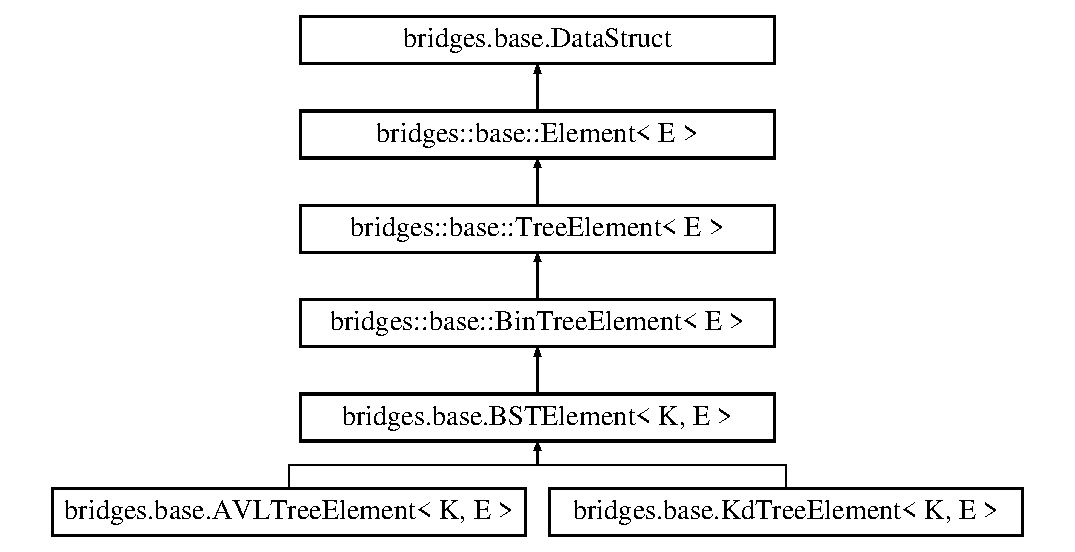
\includegraphics[height=6.000000cm]{classbridges_1_1base_1_1_b_s_t_element}
\end{center}
\end{figure}
\subsection*{Public Member Functions}
\begin{DoxyCompactItemize}
\item 
\mbox{\hyperlink{classbridges_1_1base_1_1_b_s_t_element_a5a557bf3e29e2936c244147c69e04795}{B\+S\+T\+Element}} ()
\item 
\mbox{\hyperlink{classbridges_1_1base_1_1_b_s_t_element_a0ec94ad6e2313ada05b48eb83a2f31cb}{B\+S\+T\+Element}} (E e, \mbox{\hyperlink{classbridges_1_1base_1_1_b_s_t_element}{B\+S\+T\+Element}}$<$ K, E $>$ left, \mbox{\hyperlink{classbridges_1_1base_1_1_b_s_t_element}{B\+S\+T\+Element}}$<$ K, E $>$ right)
\item 
\mbox{\hyperlink{classbridges_1_1base_1_1_b_s_t_element_a6b5bae96b241996942c467a78e6262ea}{B\+S\+T\+Element}} (K key, E e, \mbox{\hyperlink{classbridges_1_1base_1_1_b_s_t_element}{B\+S\+T\+Element}}$<$ K, E $>$ left, \mbox{\hyperlink{classbridges_1_1base_1_1_b_s_t_element}{B\+S\+T\+Element}}$<$ K, E $>$ right)
\item 
\mbox{\hyperlink{classbridges_1_1base_1_1_b_s_t_element_aa40760e586322a406841765bcf2aafc6}{B\+S\+T\+Element}} (E e)
\item 
String \mbox{\hyperlink{classbridges_1_1base_1_1_b_s_t_element_ae51e96c80d61e1a6c74f6d56a4bc2fef}{get\+Data\+Struct\+Type}} ()
\item 
\mbox{\hyperlink{classbridges_1_1base_1_1_b_s_t_element_ae19a9a445ae112673edf57a24dcf38e9}{B\+S\+T\+Element}} (K key, E e)
\item 
\mbox{\hyperlink{classbridges_1_1base_1_1_b_s_t_element_ab4a92ca5d5bdd5966bd63def8e867173}{B\+S\+T\+Element}} (String label, E e)
\item 
\mbox{\hyperlink{classbridges_1_1base_1_1_b_s_t_element_a6b76778c0c1486f599b90e51cf0a477c}{B\+S\+T\+Element}} (String label, K key, E e)
\item 
\mbox{\hyperlink{classbridges_1_1base_1_1_b_s_t_element_a067f0fcc18228e8c9427deadba9f4d96}{B\+S\+T\+Element}} (\mbox{\hyperlink{classbridges_1_1base_1_1_b_s_t_element}{B\+S\+T\+Element}}$<$ K, E $>$ left, \mbox{\hyperlink{classbridges_1_1base_1_1_b_s_t_element}{B\+S\+T\+Element}}$<$ K, E $>$ right)
\item 
K \mbox{\hyperlink{classbridges_1_1base_1_1_b_s_t_element_afba950fad36d3327b01003df3ba4cc9f}{get\+Key}} ()
\item 
void \mbox{\hyperlink{classbridges_1_1base_1_1_b_s_t_element_a51990b684df6998dc25b324dc7631ab4}{set\+Key}} (K key)
\item 
\mbox{\hyperlink{classbridges_1_1base_1_1_b_s_t_element}{B\+S\+T\+Element}}$<$ K, E $>$ \mbox{\hyperlink{classbridges_1_1base_1_1_b_s_t_element_a8abdd6e4a0486de7fa45fbb233b56688}{get\+Left}} ()
\item 
\mbox{\hyperlink{classbridges_1_1base_1_1_b_s_t_element}{B\+S\+T\+Element}}$<$ K, E $>$ \mbox{\hyperlink{classbridges_1_1base_1_1_b_s_t_element_ae7ed1b98f48acfcfc0a3a5bf6219ce00}{get\+Right}} ()
\end{DoxyCompactItemize}
\subsection*{Additional Inherited Members}


\subsection{Detailed Description}
The \mbox{\hyperlink{classbridges_1_1base_1_1_b_s_t_element}{B\+S\+T\+Element}} class is the building block for creating binary search trees. 

The \mbox{\hyperlink{classbridges_1_1base_1_1_b_s_t_element}{B\+S\+T\+Element}} class is the building block for creating binary search tree structures. It contains two children (viz., left, right), and a search key, to be used in search operations .

\mbox{\hyperlink{classbridges_1_1base_1_1_b_s_t_element}{B\+S\+T\+Element}} contains a visualizer (\mbox{\hyperlink{classbridges_1_1base_1_1_element_visualizer}{Element\+Visualizer}}) object for setting visual attributes (color, shape, opacity, size), necessary for displaying them in a web browser.

B\+ST Elements also have a \mbox{\hyperlink{classbridges_1_1base_1_1_link_visualizer}{Link\+Visualizer}} object, that is used when they are linked to another element, appropriate for setting link attributes, for instance, between the current element and its left or right child


\begin{DoxyParams}{Parameters}
{\em E} & he generic parameter object that is part of this element, representing application specific data. \\
\hline
{\em K} & is the search key parameter in the B\+ST node; K must be orderable, such as integer, float, string, etc., on which relational operators work.\\
\hline
\end{DoxyParams}
\begin{DoxyAuthor}{Author}
Kalpathi Subramanian, Mihai Mehedint
\end{DoxyAuthor}
\begin{DoxyDate}{Date}
6/22/16, 1/7/17, 5/17/17
\end{DoxyDate}
This class extends the \mbox{\hyperlink{classbridges_1_1base_1_1_bin_tree_element}{Bin\+Tree\+Element}} class by adding a \textquotesingle{}key\textquotesingle{} value for use in a binary search tree implementations.

\begin{DoxySeeAlso}{See also}
Example tutorial using \mbox{\hyperlink{classbridges_1_1base_1_1_b_s_t_element}{B\+S\+T\+Element}} at ~\newline
 \href{http://bridgesuncc.github.io/Hello_World_Tutorials/BST.html}{\tt http\+://bridgesuncc.\+github.\+io/\+Hello\+\_\+\+World\+\_\+\+Tutorials/\+B\+S\+T.\+html} 
\end{DoxySeeAlso}


\subsection{Constructor \& Destructor Documentation}
\mbox{\Hypertarget{classbridges_1_1base_1_1_b_s_t_element_a5a557bf3e29e2936c244147c69e04795}\label{classbridges_1_1base_1_1_b_s_t_element_a5a557bf3e29e2936c244147c69e04795}} 
\index{bridges\+::base\+::\+B\+S\+T\+Element@{bridges\+::base\+::\+B\+S\+T\+Element}!B\+S\+T\+Element@{B\+S\+T\+Element}}
\index{B\+S\+T\+Element@{B\+S\+T\+Element}!bridges\+::base\+::\+B\+S\+T\+Element@{bridges\+::base\+::\+B\+S\+T\+Element}}
\subsubsection{\texorpdfstring{B\+S\+T\+Element()}{BSTElement()}\hspace{0.1cm}{\footnotesize\ttfamily [1/8]}}
{\footnotesize\ttfamily \mbox{\hyperlink{classbridges_1_1base_1_1_b_s_t_element}{bridges.\+base.\+B\+S\+T\+Element}}$<$ K, E $>$.\mbox{\hyperlink{classbridges_1_1base_1_1_b_s_t_element}{B\+S\+T\+Element}} (\begin{DoxyParamCaption}{ }\end{DoxyParamCaption})}

Construct an empty \mbox{\hyperlink{classbridges_1_1base_1_1_b_s_t_element}{B\+S\+T\+Element}} with no key assigned and left and right pointers set to null. \mbox{\Hypertarget{classbridges_1_1base_1_1_b_s_t_element_a0ec94ad6e2313ada05b48eb83a2f31cb}\label{classbridges_1_1base_1_1_b_s_t_element_a0ec94ad6e2313ada05b48eb83a2f31cb}} 
\index{bridges\+::base\+::\+B\+S\+T\+Element@{bridges\+::base\+::\+B\+S\+T\+Element}!B\+S\+T\+Element@{B\+S\+T\+Element}}
\index{B\+S\+T\+Element@{B\+S\+T\+Element}!bridges\+::base\+::\+B\+S\+T\+Element@{bridges\+::base\+::\+B\+S\+T\+Element}}
\subsubsection{\texorpdfstring{B\+S\+T\+Element()}{BSTElement()}\hspace{0.1cm}{\footnotesize\ttfamily [2/8]}}
{\footnotesize\ttfamily \mbox{\hyperlink{classbridges_1_1base_1_1_b_s_t_element}{bridges.\+base.\+B\+S\+T\+Element}}$<$ K, E $>$.\mbox{\hyperlink{classbridges_1_1base_1_1_b_s_t_element}{B\+S\+T\+Element}} (\begin{DoxyParamCaption}\item[{E}]{e,  }\item[{\mbox{\hyperlink{classbridges_1_1base_1_1_b_s_t_element}{B\+S\+T\+Element}}$<$ K, E $>$}]{left,  }\item[{\mbox{\hyperlink{classbridges_1_1base_1_1_b_s_t_element}{B\+S\+T\+Element}}$<$ K, E $>$}]{right }\end{DoxyParamCaption})}

Construct a \mbox{\hyperlink{classbridges_1_1base_1_1_b_s_t_element}{B\+S\+T\+Element}} holding an object \char`\"{}e\char`\"{} with a left pointer assigned to \char`\"{}left\char`\"{} and a right pointer assigned to \char`\"{}right\char`\"{}. 
\begin{DoxyParams}{Parameters}
{\em e} & the object that \mbox{\hyperlink{classbridges_1_1base_1_1_b_s_t_element}{B\+S\+T\+Element}} is holding \\
\hline
{\em left} & the \mbox{\hyperlink{classbridges_1_1base_1_1_b_s_t_element}{B\+S\+T\+Element}} that should be assigned to the left pointer \\
\hline
{\em right} & the B\+S\+T\+Elemetn taht should be assigned to the right pointer \\
\hline
\end{DoxyParams}
\mbox{\Hypertarget{classbridges_1_1base_1_1_b_s_t_element_a6b5bae96b241996942c467a78e6262ea}\label{classbridges_1_1base_1_1_b_s_t_element_a6b5bae96b241996942c467a78e6262ea}} 
\index{bridges\+::base\+::\+B\+S\+T\+Element@{bridges\+::base\+::\+B\+S\+T\+Element}!B\+S\+T\+Element@{B\+S\+T\+Element}}
\index{B\+S\+T\+Element@{B\+S\+T\+Element}!bridges\+::base\+::\+B\+S\+T\+Element@{bridges\+::base\+::\+B\+S\+T\+Element}}
\subsubsection{\texorpdfstring{B\+S\+T\+Element()}{BSTElement()}\hspace{0.1cm}{\footnotesize\ttfamily [3/8]}}
{\footnotesize\ttfamily \mbox{\hyperlink{classbridges_1_1base_1_1_b_s_t_element}{bridges.\+base.\+B\+S\+T\+Element}}$<$ K, E $>$.\mbox{\hyperlink{classbridges_1_1base_1_1_b_s_t_element}{B\+S\+T\+Element}} (\begin{DoxyParamCaption}\item[{K}]{key,  }\item[{E}]{e,  }\item[{\mbox{\hyperlink{classbridges_1_1base_1_1_b_s_t_element}{B\+S\+T\+Element}}$<$ K, E $>$}]{left,  }\item[{\mbox{\hyperlink{classbridges_1_1base_1_1_b_s_t_element}{B\+S\+T\+Element}}$<$ K, E $>$}]{right }\end{DoxyParamCaption})}

Construct a \mbox{\hyperlink{classbridges_1_1base_1_1_b_s_t_element}{B\+S\+T\+Element}} with a key \char`\"{}key\char`\"{}, holding an object \char`\"{}e\char`\"{} with a left pointer assigned to \char`\"{}left\char`\"{} and a right pointer assigned to \char`\"{}right\char`\"{}.


\begin{DoxyParams}{Parameters}
{\em key} & the key to be used in a binary search tree implementation \\
\hline
{\em e} & the object this \mbox{\hyperlink{classbridges_1_1base_1_1_b_s_t_element}{B\+S\+T\+Element}} is holding \\
\hline
{\em left} & the \mbox{\hyperlink{classbridges_1_1base_1_1_b_s_t_element}{B\+S\+T\+Element}} that should be assigned to the left pointer \\
\hline
{\em right} & the \mbox{\hyperlink{classbridges_1_1base_1_1_b_s_t_element}{B\+S\+T\+Element}} that should be assigned to the right pointer \\
\hline
\end{DoxyParams}
\mbox{\Hypertarget{classbridges_1_1base_1_1_b_s_t_element_aa40760e586322a406841765bcf2aafc6}\label{classbridges_1_1base_1_1_b_s_t_element_aa40760e586322a406841765bcf2aafc6}} 
\index{bridges\+::base\+::\+B\+S\+T\+Element@{bridges\+::base\+::\+B\+S\+T\+Element}!B\+S\+T\+Element@{B\+S\+T\+Element}}
\index{B\+S\+T\+Element@{B\+S\+T\+Element}!bridges\+::base\+::\+B\+S\+T\+Element@{bridges\+::base\+::\+B\+S\+T\+Element}}
\subsubsection{\texorpdfstring{B\+S\+T\+Element()}{BSTElement()}\hspace{0.1cm}{\footnotesize\ttfamily [4/8]}}
{\footnotesize\ttfamily \mbox{\hyperlink{classbridges_1_1base_1_1_b_s_t_element}{bridges.\+base.\+B\+S\+T\+Element}}$<$ K, E $>$.\mbox{\hyperlink{classbridges_1_1base_1_1_b_s_t_element}{B\+S\+T\+Element}} (\begin{DoxyParamCaption}\item[{E}]{e }\end{DoxyParamCaption})}

Construct a \mbox{\hyperlink{classbridges_1_1base_1_1_b_s_t_element}{B\+S\+T\+Element}} holding the object \char`\"{}e\char`\"{}, with no key assigned and left and right pointers set to null.


\begin{DoxyParams}{Parameters}
{\em e} & the object this \mbox{\hyperlink{classbridges_1_1base_1_1_b_s_t_element}{B\+S\+T\+Element}} is holding \\
\hline
\end{DoxyParams}
\mbox{\Hypertarget{classbridges_1_1base_1_1_b_s_t_element_ae19a9a445ae112673edf57a24dcf38e9}\label{classbridges_1_1base_1_1_b_s_t_element_ae19a9a445ae112673edf57a24dcf38e9}} 
\index{bridges\+::base\+::\+B\+S\+T\+Element@{bridges\+::base\+::\+B\+S\+T\+Element}!B\+S\+T\+Element@{B\+S\+T\+Element}}
\index{B\+S\+T\+Element@{B\+S\+T\+Element}!bridges\+::base\+::\+B\+S\+T\+Element@{bridges\+::base\+::\+B\+S\+T\+Element}}
\subsubsection{\texorpdfstring{B\+S\+T\+Element()}{BSTElement()}\hspace{0.1cm}{\footnotesize\ttfamily [5/8]}}
{\footnotesize\ttfamily \mbox{\hyperlink{classbridges_1_1base_1_1_b_s_t_element}{bridges.\+base.\+B\+S\+T\+Element}}$<$ K, E $>$.\mbox{\hyperlink{classbridges_1_1base_1_1_b_s_t_element}{B\+S\+T\+Element}} (\begin{DoxyParamCaption}\item[{K}]{key,  }\item[{E}]{e }\end{DoxyParamCaption})}

Construct a \mbox{\hyperlink{classbridges_1_1base_1_1_b_s_t_element}{B\+S\+T\+Element}} holding the object \char`\"{}e\char`\"{}, with key \char`\"{}key\char`\"{} assigned and left and right pointers set to null. 
\begin{DoxyParams}{Parameters}
{\em key} & the key to be used in a binary search tree implementation \\
\hline
{\em e} & the object this \mbox{\hyperlink{classbridges_1_1base_1_1_b_s_t_element}{B\+S\+T\+Element}} is holding \\
\hline
\end{DoxyParams}
\mbox{\Hypertarget{classbridges_1_1base_1_1_b_s_t_element_ab4a92ca5d5bdd5966bd63def8e867173}\label{classbridges_1_1base_1_1_b_s_t_element_ab4a92ca5d5bdd5966bd63def8e867173}} 
\index{bridges\+::base\+::\+B\+S\+T\+Element@{bridges\+::base\+::\+B\+S\+T\+Element}!B\+S\+T\+Element@{B\+S\+T\+Element}}
\index{B\+S\+T\+Element@{B\+S\+T\+Element}!bridges\+::base\+::\+B\+S\+T\+Element@{bridges\+::base\+::\+B\+S\+T\+Element}}
\subsubsection{\texorpdfstring{B\+S\+T\+Element()}{BSTElement()}\hspace{0.1cm}{\footnotesize\ttfamily [6/8]}}
{\footnotesize\ttfamily \mbox{\hyperlink{classbridges_1_1base_1_1_b_s_t_element}{bridges.\+base.\+B\+S\+T\+Element}}$<$ K, E $>$.\mbox{\hyperlink{classbridges_1_1base_1_1_b_s_t_element}{B\+S\+T\+Element}} (\begin{DoxyParamCaption}\item[{String}]{label,  }\item[{E}]{e }\end{DoxyParamCaption})}

Construct a \mbox{\hyperlink{classbridges_1_1base_1_1_b_s_t_element}{B\+S\+T\+Element}} holding the object \char`\"{}e\char`\"{}, with label set to \char`\"{}label\char`\"{}, with no key assigned, and left and right pointers set to null. 
\begin{DoxyParams}{Parameters}
{\em label} & the label of \mbox{\hyperlink{classbridges_1_1base_1_1_b_s_t_element}{B\+S\+T\+Element}} that shows up on the Bridges visualization \\
\hline
{\em e} & the object this \mbox{\hyperlink{classbridges_1_1base_1_1_b_s_t_element}{B\+S\+T\+Element}} is holding \\
\hline
\end{DoxyParams}
\mbox{\Hypertarget{classbridges_1_1base_1_1_b_s_t_element_a6b76778c0c1486f599b90e51cf0a477c}\label{classbridges_1_1base_1_1_b_s_t_element_a6b76778c0c1486f599b90e51cf0a477c}} 
\index{bridges\+::base\+::\+B\+S\+T\+Element@{bridges\+::base\+::\+B\+S\+T\+Element}!B\+S\+T\+Element@{B\+S\+T\+Element}}
\index{B\+S\+T\+Element@{B\+S\+T\+Element}!bridges\+::base\+::\+B\+S\+T\+Element@{bridges\+::base\+::\+B\+S\+T\+Element}}
\subsubsection{\texorpdfstring{B\+S\+T\+Element()}{BSTElement()}\hspace{0.1cm}{\footnotesize\ttfamily [7/8]}}
{\footnotesize\ttfamily \mbox{\hyperlink{classbridges_1_1base_1_1_b_s_t_element}{bridges.\+base.\+B\+S\+T\+Element}}$<$ K, E $>$.\mbox{\hyperlink{classbridges_1_1base_1_1_b_s_t_element}{B\+S\+T\+Element}} (\begin{DoxyParamCaption}\item[{String}]{label,  }\item[{K}]{key,  }\item[{E}]{e }\end{DoxyParamCaption})}

Construct a \mbox{\hyperlink{classbridges_1_1base_1_1_b_s_t_element}{B\+S\+T\+Element}} holding the object \char`\"{}e\char`\"{}, with label set to \char`\"{}label\char`\"{}, with \char`\"{}key\char`\"{} assigned to key, and left and right pointers set to null.


\begin{DoxyParams}{Parameters}
{\em label} & the label of \mbox{\hyperlink{classbridges_1_1base_1_1_b_s_t_element}{B\+S\+T\+Element}} that shows up on the Bridges visualization \\
\hline
{\em key} & the key to be used in a binary search tree implementation \\
\hline
{\em e} & the object this \mbox{\hyperlink{classbridges_1_1base_1_1_b_s_t_element}{B\+S\+T\+Element}} is holding \\
\hline
\end{DoxyParams}
\mbox{\Hypertarget{classbridges_1_1base_1_1_b_s_t_element_a067f0fcc18228e8c9427deadba9f4d96}\label{classbridges_1_1base_1_1_b_s_t_element_a067f0fcc18228e8c9427deadba9f4d96}} 
\index{bridges\+::base\+::\+B\+S\+T\+Element@{bridges\+::base\+::\+B\+S\+T\+Element}!B\+S\+T\+Element@{B\+S\+T\+Element}}
\index{B\+S\+T\+Element@{B\+S\+T\+Element}!bridges\+::base\+::\+B\+S\+T\+Element@{bridges\+::base\+::\+B\+S\+T\+Element}}
\subsubsection{\texorpdfstring{B\+S\+T\+Element()}{BSTElement()}\hspace{0.1cm}{\footnotesize\ttfamily [8/8]}}
{\footnotesize\ttfamily \mbox{\hyperlink{classbridges_1_1base_1_1_b_s_t_element}{bridges.\+base.\+B\+S\+T\+Element}}$<$ K, E $>$.\mbox{\hyperlink{classbridges_1_1base_1_1_b_s_t_element}{B\+S\+T\+Element}} (\begin{DoxyParamCaption}\item[{\mbox{\hyperlink{classbridges_1_1base_1_1_b_s_t_element}{B\+S\+T\+Element}}$<$ K, E $>$}]{left,  }\item[{\mbox{\hyperlink{classbridges_1_1base_1_1_b_s_t_element}{B\+S\+T\+Element}}$<$ K, E $>$}]{right }\end{DoxyParamCaption})}

Construct an empty \mbox{\hyperlink{classbridges_1_1base_1_1_b_s_t_element}{B\+S\+T\+Element}}, with no key assigned, and left and right pointers set to null. 
\begin{DoxyParams}{Parameters}
{\em left} & the \mbox{\hyperlink{classbridges_1_1base_1_1_b_s_t_element}{B\+S\+T\+Element}} that should be assigned to the left pointer \\
\hline
{\em right} & the \mbox{\hyperlink{classbridges_1_1base_1_1_b_s_t_element}{B\+S\+T\+Element}} that should be assigned to the right pointer \\
\hline
\end{DoxyParams}


\subsection{Member Function Documentation}
\mbox{\Hypertarget{classbridges_1_1base_1_1_b_s_t_element_ae51e96c80d61e1a6c74f6d56a4bc2fef}\label{classbridges_1_1base_1_1_b_s_t_element_ae51e96c80d61e1a6c74f6d56a4bc2fef}} 
\index{bridges\+::base\+::\+B\+S\+T\+Element@{bridges\+::base\+::\+B\+S\+T\+Element}!get\+Data\+Struct\+Type@{get\+Data\+Struct\+Type}}
\index{get\+Data\+Struct\+Type@{get\+Data\+Struct\+Type}!bridges\+::base\+::\+B\+S\+T\+Element@{bridges\+::base\+::\+B\+S\+T\+Element}}
\subsubsection{\texorpdfstring{get\+Data\+Struct\+Type()}{getDataStructType()}}
{\footnotesize\ttfamily String \mbox{\hyperlink{classbridges_1_1base_1_1_b_s_t_element}{bridges.\+base.\+B\+S\+T\+Element}}$<$ K, E $>$.get\+Data\+Struct\+Type (\begin{DoxyParamCaption}{ }\end{DoxyParamCaption})}

This method gets the data structure type

\begin{DoxyReturn}{Returns}
The date structure type as a string 
\end{DoxyReturn}
\mbox{\Hypertarget{classbridges_1_1base_1_1_b_s_t_element_afba950fad36d3327b01003df3ba4cc9f}\label{classbridges_1_1base_1_1_b_s_t_element_afba950fad36d3327b01003df3ba4cc9f}} 
\index{bridges\+::base\+::\+B\+S\+T\+Element@{bridges\+::base\+::\+B\+S\+T\+Element}!get\+Key@{get\+Key}}
\index{get\+Key@{get\+Key}!bridges\+::base\+::\+B\+S\+T\+Element@{bridges\+::base\+::\+B\+S\+T\+Element}}
\subsubsection{\texorpdfstring{get\+Key()}{getKey()}}
{\footnotesize\ttfamily K \mbox{\hyperlink{classbridges_1_1base_1_1_b_s_t_element}{bridges.\+base.\+B\+S\+T\+Element}}$<$ K, E $>$.get\+Key (\begin{DoxyParamCaption}{ }\end{DoxyParamCaption})}

Return the key of the \mbox{\hyperlink{classbridges_1_1base_1_1_b_s_t_element}{B\+S\+T\+Element}}

\begin{DoxyReturn}{Returns}
the key of this \mbox{\hyperlink{classbridges_1_1base_1_1_b_s_t_element}{B\+S\+T\+Element}} 
\end{DoxyReturn}
\mbox{\Hypertarget{classbridges_1_1base_1_1_b_s_t_element_a8abdd6e4a0486de7fa45fbb233b56688}\label{classbridges_1_1base_1_1_b_s_t_element_a8abdd6e4a0486de7fa45fbb233b56688}} 
\index{bridges\+::base\+::\+B\+S\+T\+Element@{bridges\+::base\+::\+B\+S\+T\+Element}!get\+Left@{get\+Left}}
\index{get\+Left@{get\+Left}!bridges\+::base\+::\+B\+S\+T\+Element@{bridges\+::base\+::\+B\+S\+T\+Element}}
\subsubsection{\texorpdfstring{get\+Left()}{getLeft()}}
{\footnotesize\ttfamily \mbox{\hyperlink{classbridges_1_1base_1_1_b_s_t_element}{B\+S\+T\+Element}}$<$K, E$>$ \mbox{\hyperlink{classbridges_1_1base_1_1_b_s_t_element}{bridges.\+base.\+B\+S\+T\+Element}}$<$ K, E $>$.get\+Left (\begin{DoxyParamCaption}{ }\end{DoxyParamCaption})}

\mbox{\Hypertarget{classbridges_1_1base_1_1_b_s_t_element_ae7ed1b98f48acfcfc0a3a5bf6219ce00}\label{classbridges_1_1base_1_1_b_s_t_element_ae7ed1b98f48acfcfc0a3a5bf6219ce00}} 
\index{bridges\+::base\+::\+B\+S\+T\+Element@{bridges\+::base\+::\+B\+S\+T\+Element}!get\+Right@{get\+Right}}
\index{get\+Right@{get\+Right}!bridges\+::base\+::\+B\+S\+T\+Element@{bridges\+::base\+::\+B\+S\+T\+Element}}
\subsubsection{\texorpdfstring{get\+Right()}{getRight()}}
{\footnotesize\ttfamily \mbox{\hyperlink{classbridges_1_1base_1_1_b_s_t_element}{B\+S\+T\+Element}}$<$K, E$>$ \mbox{\hyperlink{classbridges_1_1base_1_1_b_s_t_element}{bridges.\+base.\+B\+S\+T\+Element}}$<$ K, E $>$.get\+Right (\begin{DoxyParamCaption}{ }\end{DoxyParamCaption})}

\mbox{\Hypertarget{classbridges_1_1base_1_1_b_s_t_element_a51990b684df6998dc25b324dc7631ab4}\label{classbridges_1_1base_1_1_b_s_t_element_a51990b684df6998dc25b324dc7631ab4}} 
\index{bridges\+::base\+::\+B\+S\+T\+Element@{bridges\+::base\+::\+B\+S\+T\+Element}!set\+Key@{set\+Key}}
\index{set\+Key@{set\+Key}!bridges\+::base\+::\+B\+S\+T\+Element@{bridges\+::base\+::\+B\+S\+T\+Element}}
\subsubsection{\texorpdfstring{set\+Key()}{setKey()}}
{\footnotesize\ttfamily void \mbox{\hyperlink{classbridges_1_1base_1_1_b_s_t_element}{bridges.\+base.\+B\+S\+T\+Element}}$<$ K, E $>$.set\+Key (\begin{DoxyParamCaption}\item[{K}]{key }\end{DoxyParamCaption})}

Set the key of the \mbox{\hyperlink{classbridges_1_1base_1_1_b_s_t_element}{B\+S\+T\+Element}} to key 
\begin{DoxyParams}{Parameters}
{\em key} & the key to set \\
\hline
\end{DoxyParams}


The documentation for this class was generated from the following file\+:\begin{DoxyCompactItemize}
\item 
/\+Users/kalpathi/gr/bridges/client/java/bridges-\/17/src/main/java/edu/uncc/cs/bridges\+\_\+v21/base/\mbox{\hyperlink{_b_s_t_element_8java}{B\+S\+T\+Element.\+java}}\end{DoxyCompactItemize}

\hypertarget{classbridges_1_1data__src__dependent_1_1_cancer_incidence}{}\section{bridges.\+data\+\_\+src\+\_\+dependent.\+Cancer\+Incidence Class Reference}
\label{classbridges_1_1data__src__dependent_1_1_cancer_incidence}\index{bridges.\+data\+\_\+src\+\_\+dependent.\+Cancer\+Incidence@{bridges.\+data\+\_\+src\+\_\+dependent.\+Cancer\+Incidence}}


Inherits bridges.\+data\+\_\+src\+\_\+dependent.\+Data\+Source.



\subsection{Detailed Description}
United States Cancer Statistics from the U.\+S. Center for Disease Control. 

From the United States Cancer Statistics as part of the U.\+S. Center for Disease Control, the following data set focuses on the crude rate for all types of cancer reported for different demograpic groups. Significant groupings include age, gender, race and geographical area.

\href{http://www.cdc.gov/cancer/npcr/uscs/download_data.htm}{\tt http\+://www.\+cdc.\+gov/cancer/npcr/uscs/download\+\_\+data.\+htm} Data\+: Courtesy of Corgis Datasets, 2017

Author\+: Kalpathi Subramanian, April, 2017 \subsection*{Public Member Functions}
\begin{DoxyCompactItemize}
\item 
\hyperlink{classbridges_1_1data__src__dependent_1_1_cancer_incidence_a92db1eb4292c77f07619019587caf5cc}{Cancer\+Incidence} ()
\item 
\hyperlink{classbridges_1_1data__src__dependent_1_1_cancer_incidence_a3db553c2769892563c3f1ebb033ba4c6}{Cancer\+Incidence} (String canc\+\_\+label)
\item 
String \hyperlink{classbridges_1_1data__src__dependent_1_1_cancer_incidence_ac7958f37807979cf06e712373f080b9a}{get\+Name} ()
\begin{DoxyCompactList}\small\item\em get the name of the incidence report. \end{DoxyCompactList}\item 
void \hyperlink{classbridges_1_1data__src__dependent_1_1_cancer_incidence_a1aef58b128adfd1e2a31ab9726247e9e}{set\+Name} (String name)
\begin{DoxyCompactList}\small\item\em sets the string name \end{DoxyCompactList}\item 
double \hyperlink{classbridges_1_1data__src__dependent_1_1_cancer_incidence_a87bc1cbc5a72eb9b4df5ff7ab4843ae8}{get\+Age\+Adjusted\+Rate} ()
\item 
void \hyperlink{classbridges_1_1data__src__dependent_1_1_cancer_incidence_a26c2d63e8465bcfdab047129312b4897}{set\+Age\+Adjusted\+Rate} (double aar)
\begin{DoxyCompactList}\small\item\em Set age adjusted cancer rate. \end{DoxyCompactList}\item 
double \hyperlink{classbridges_1_1data__src__dependent_1_1_cancer_incidence_a7e5dab6d140f2a8e162c5d5c514c74c1}{get\+Age\+Adjusted\+C\+I\+\_\+\+Lower} ()
\item 
void \hyperlink{classbridges_1_1data__src__dependent_1_1_cancer_incidence_a4cd8ce7c68f00d2cd15928764cc32c09}{set\+Age\+Adjusted\+C\+I\+\_\+\+Lower} (double ci\+\_\+l)
\begin{DoxyCompactList}\small\item\em Set age adjusted cancer conf interval (lower) \end{DoxyCompactList}\item 
double \hyperlink{classbridges_1_1data__src__dependent_1_1_cancer_incidence_ae7b71d91c3acae9fce3536f6a9d8362b}{get\+Age\+Adjusted\+C\+I\+\_\+\+Upper} ()
\item 
void \hyperlink{classbridges_1_1data__src__dependent_1_1_cancer_incidence_aeb386486bfbd96ba9ab689b7d95d4522}{set\+Age\+Adjusted\+C\+I\+\_\+\+Upper} (double ci\+\_\+u)
\begin{DoxyCompactList}\small\item\em Set age adjusted cancer conf interval (upper) \end{DoxyCompactList}\item 
double \hyperlink{classbridges_1_1data__src__dependent_1_1_cancer_incidence_afc2ddb3099dffc46371ad7188278501d}{get\+Crude\+Rate} ()
\begin{DoxyCompactList}\small\item\em Get the cancer rate, adjusted for population. \end{DoxyCompactList}\item 
void \hyperlink{classbridges_1_1data__src__dependent_1_1_cancer_incidence_a64a737fd7481262650efd596c508ffd6}{set\+Crude\+Rate} (double cr)
\begin{DoxyCompactList}\small\item\em Set cancer rate, adjusted for population. \end{DoxyCompactList}\item 
double \hyperlink{classbridges_1_1data__src__dependent_1_1_cancer_incidence_a8c410730b03abc78395e75b5024d495e}{get\+Crude\+Rate\+\_\+\+C\+I\+\_\+\+Lower} ()
\begin{DoxyCompactList}\small\item\em Get the expected cancer crude rate confidence interval(lower), adjusted for age of participants. \end{DoxyCompactList}\item 
void \hyperlink{classbridges_1_1data__src__dependent_1_1_cancer_incidence_a72e3960af58f32d26e32f49ada2f1555}{set\+Crude\+Rate\+\_\+\+C\+I\+\_\+\+Lower} (double cr\+\_\+l)
\begin{DoxyCompactList}\small\item\em Set age adjusted cancer crude conf interval (lower) \end{DoxyCompactList}\item 
double \hyperlink{classbridges_1_1data__src__dependent_1_1_cancer_incidence_a4ca1ceed275ab6371f861d3a03975f15}{get\+Crude\+Rate\+\_\+\+C\+I\+\_\+\+Upper} ()
\item 
void \hyperlink{classbridges_1_1data__src__dependent_1_1_cancer_incidence_a99e25dd53093badf350b06b7e0c8b725}{set\+Crude\+Rate\+\_\+\+C\+I\+\_\+\+Upper} (double cr\+\_\+u)
\begin{DoxyCompactList}\small\item\em Set crude rate CI (upper) \end{DoxyCompactList}\item 
int \hyperlink{classbridges_1_1data__src__dependent_1_1_cancer_incidence_aaff714019154afa796d54ed57ffc9492}{get\+Year} ()
\begin{DoxyCompactList}\small\item\em Get the year of this cancer record. \end{DoxyCompactList}\item 
void \hyperlink{classbridges_1_1data__src__dependent_1_1_cancer_incidence_aa5524736b76d67f1248d1a05d9f596a9}{set\+Year} (int y)
\begin{DoxyCompactList}\small\item\em Set the year of this cancer record. \end{DoxyCompactList}\item 
String \hyperlink{classbridges_1_1data__src__dependent_1_1_cancer_incidence_a2c3cbe65d89827c167f15314b8b088b3}{get\+Gender} ()
\item 
void \hyperlink{classbridges_1_1data__src__dependent_1_1_cancer_incidence_a217681578e13197e1d177932c73ea80f}{set\+Gender} (String g)
\begin{DoxyCompactList}\small\item\em Set gender. \end{DoxyCompactList}\item 
String \hyperlink{classbridges_1_1data__src__dependent_1_1_cancer_incidence_a18de1c14d36cd7656555c8465ea8a009}{get\+Race} ()
\item 
void \hyperlink{classbridges_1_1data__src__dependent_1_1_cancer_incidence_a8c26c4358561453f3d2ca3a463eed872}{set\+Race} (String r)
\begin{DoxyCompactList}\small\item\em Set race. \end{DoxyCompactList}\item 
String \hyperlink{classbridges_1_1data__src__dependent_1_1_cancer_incidence_a844c6c3317bdb6b124f32b40804e1ff7}{get\+Event\+Type} ()
\begin{DoxyCompactList}\small\item\em Get the event type (incidence, mortality, etc) \end{DoxyCompactList}\item 
void \hyperlink{classbridges_1_1data__src__dependent_1_1_cancer_incidence_a39338b20223e60b79fa38b3034ca46b7}{set\+Event\+Type} (String et)
\begin{DoxyCompactList}\small\item\em Set event type. \end{DoxyCompactList}\item 
int \hyperlink{classbridges_1_1data__src__dependent_1_1_cancer_incidence_a41c2507d46589080f6bb76ab29f53665}{get\+Population} ()
\begin{DoxyCompactList}\small\item\em Get the population size. \end{DoxyCompactList}\item 
void \hyperlink{classbridges_1_1data__src__dependent_1_1_cancer_incidence_a9f1caf002b6573aa699a81ed1b835af0}{set\+Population} (int pop)
\begin{DoxyCompactList}\small\item\em Set population size. \end{DoxyCompactList}\item 
String \hyperlink{classbridges_1_1data__src__dependent_1_1_cancer_incidence_ad4c0c709fa5da9c0f20b648052db5f26}{get\+Affected\+Area} ()
\begin{DoxyCompactList}\small\item\em Get the cancer incidence area (state, region, etc) \end{DoxyCompactList}\item 
void \hyperlink{classbridges_1_1data__src__dependent_1_1_cancer_incidence_a9c7f2d303da9498e5e6145439c5a6fbc}{set\+Affected\+Area} (String area)
\begin{DoxyCompactList}\small\item\em Set cancer incidence area. \end{DoxyCompactList}\item 
int \hyperlink{classbridges_1_1data__src__dependent_1_1_cancer_incidence_a8769cb18ddb590dc41a04a220174f3df}{get\+Count} ()
\begin{DoxyCompactList}\small\item\em Get the number of people affected in this group. \end{DoxyCompactList}\item 
void \hyperlink{classbridges_1_1data__src__dependent_1_1_cancer_incidence_a18099439ef6e35cf240b06f0e0158c72}{set\+Count} (int c)
\begin{DoxyCompactList}\small\item\em Set cancer incidence count. \end{DoxyCompactList}\item 
double \hyperlink{classbridges_1_1data__src__dependent_1_1_cancer_incidence_a24aa8144dcacd93a26c3c033471666df}{get\+LocationX} ()
\begin{DoxyCompactList}\small\item\em Get the X coordinate of location. \end{DoxyCompactList}\item 
void \hyperlink{classbridges_1_1data__src__dependent_1_1_cancer_incidence_a384149c413173fba51adad1b1769797a}{set\+LocationX} (double locX)
\begin{DoxyCompactList}\small\item\em Set location (X coord) \end{DoxyCompactList}\item 
double \hyperlink{classbridges_1_1data__src__dependent_1_1_cancer_incidence_a53b56a9931a1d02ee356c6258e245aa8}{get\+LocationY} ()
\begin{DoxyCompactList}\small\item\em Get the Y coordinate of location. \end{DoxyCompactList}\item 
void \hyperlink{classbridges_1_1data__src__dependent_1_1_cancer_incidence_a14c6921a71834c14d561bc7f2aa8a18e}{set\+LocationY} (double locY)
\begin{DoxyCompactList}\small\item\em Set location (Y coord) \end{DoxyCompactList}\end{DoxyCompactItemize}


\subsection{Constructor \& Destructor Documentation}
\mbox{\Hypertarget{classbridges_1_1data__src__dependent_1_1_cancer_incidence_a92db1eb4292c77f07619019587caf5cc}\label{classbridges_1_1data__src__dependent_1_1_cancer_incidence_a92db1eb4292c77f07619019587caf5cc}} 
\index{bridges\+::data\+\_\+src\+\_\+dependent\+::\+Cancer\+Incidence@{bridges\+::data\+\_\+src\+\_\+dependent\+::\+Cancer\+Incidence}!Cancer\+Incidence@{Cancer\+Incidence}}
\index{Cancer\+Incidence@{Cancer\+Incidence}!bridges\+::data\+\_\+src\+\_\+dependent\+::\+Cancer\+Incidence@{bridges\+::data\+\_\+src\+\_\+dependent\+::\+Cancer\+Incidence}}
\subsubsection{\texorpdfstring{Cancer\+Incidence()}{CancerIncidence()}\hspace{0.1cm}{\footnotesize\ttfamily [1/2]}}
{\footnotesize\ttfamily bridges.\+data\+\_\+src\+\_\+dependent.\+Cancer\+Incidence.\+Cancer\+Incidence (\begin{DoxyParamCaption}{ }\end{DoxyParamCaption})}

\mbox{\Hypertarget{classbridges_1_1data__src__dependent_1_1_cancer_incidence_a3db553c2769892563c3f1ebb033ba4c6}\label{classbridges_1_1data__src__dependent_1_1_cancer_incidence_a3db553c2769892563c3f1ebb033ba4c6}} 
\index{bridges\+::data\+\_\+src\+\_\+dependent\+::\+Cancer\+Incidence@{bridges\+::data\+\_\+src\+\_\+dependent\+::\+Cancer\+Incidence}!Cancer\+Incidence@{Cancer\+Incidence}}
\index{Cancer\+Incidence@{Cancer\+Incidence}!bridges\+::data\+\_\+src\+\_\+dependent\+::\+Cancer\+Incidence@{bridges\+::data\+\_\+src\+\_\+dependent\+::\+Cancer\+Incidence}}
\subsubsection{\texorpdfstring{Cancer\+Incidence()}{CancerIncidence()}\hspace{0.1cm}{\footnotesize\ttfamily [2/2]}}
{\footnotesize\ttfamily bridges.\+data\+\_\+src\+\_\+dependent.\+Cancer\+Incidence.\+Cancer\+Incidence (\begin{DoxyParamCaption}\item[{String}]{canc\+\_\+label }\end{DoxyParamCaption})}



\subsection{Member Function Documentation}
\mbox{\Hypertarget{classbridges_1_1data__src__dependent_1_1_cancer_incidence_ad4c0c709fa5da9c0f20b648052db5f26}\label{classbridges_1_1data__src__dependent_1_1_cancer_incidence_ad4c0c709fa5da9c0f20b648052db5f26}} 
\index{bridges\+::data\+\_\+src\+\_\+dependent\+::\+Cancer\+Incidence@{bridges\+::data\+\_\+src\+\_\+dependent\+::\+Cancer\+Incidence}!get\+Affected\+Area@{get\+Affected\+Area}}
\index{get\+Affected\+Area@{get\+Affected\+Area}!bridges\+::data\+\_\+src\+\_\+dependent\+::\+Cancer\+Incidence@{bridges\+::data\+\_\+src\+\_\+dependent\+::\+Cancer\+Incidence}}
\subsubsection{\texorpdfstring{get\+Affected\+Area()}{getAffectedArea()}}
{\footnotesize\ttfamily String bridges.\+data\+\_\+src\+\_\+dependent.\+Cancer\+Incidence.\+get\+Affected\+Area (\begin{DoxyParamCaption}{ }\end{DoxyParamCaption})}



Get the cancer incidence area (state, region, etc) 

\begin{DoxyReturn}{Returns}
affected area 
\end{DoxyReturn}
\mbox{\Hypertarget{classbridges_1_1data__src__dependent_1_1_cancer_incidence_a7e5dab6d140f2a8e162c5d5c514c74c1}\label{classbridges_1_1data__src__dependent_1_1_cancer_incidence_a7e5dab6d140f2a8e162c5d5c514c74c1}} 
\index{bridges\+::data\+\_\+src\+\_\+dependent\+::\+Cancer\+Incidence@{bridges\+::data\+\_\+src\+\_\+dependent\+::\+Cancer\+Incidence}!get\+Age\+Adjusted\+C\+I\+\_\+\+Lower@{get\+Age\+Adjusted\+C\+I\+\_\+\+Lower}}
\index{get\+Age\+Adjusted\+C\+I\+\_\+\+Lower@{get\+Age\+Adjusted\+C\+I\+\_\+\+Lower}!bridges\+::data\+\_\+src\+\_\+dependent\+::\+Cancer\+Incidence@{bridges\+::data\+\_\+src\+\_\+dependent\+::\+Cancer\+Incidence}}
\subsubsection{\texorpdfstring{get\+Age\+Adjusted\+C\+I\+\_\+\+Lower()}{getAgeAdjustedCI\_Lower()}}
{\footnotesize\ttfamily double bridges.\+data\+\_\+src\+\_\+dependent.\+Cancer\+Incidence.\+get\+Age\+Adjusted\+C\+I\+\_\+\+Lower (\begin{DoxyParamCaption}{ }\end{DoxyParamCaption})}

\mbox{\Hypertarget{classbridges_1_1data__src__dependent_1_1_cancer_incidence_ae7b71d91c3acae9fce3536f6a9d8362b}\label{classbridges_1_1data__src__dependent_1_1_cancer_incidence_ae7b71d91c3acae9fce3536f6a9d8362b}} 
\index{bridges\+::data\+\_\+src\+\_\+dependent\+::\+Cancer\+Incidence@{bridges\+::data\+\_\+src\+\_\+dependent\+::\+Cancer\+Incidence}!get\+Age\+Adjusted\+C\+I\+\_\+\+Upper@{get\+Age\+Adjusted\+C\+I\+\_\+\+Upper}}
\index{get\+Age\+Adjusted\+C\+I\+\_\+\+Upper@{get\+Age\+Adjusted\+C\+I\+\_\+\+Upper}!bridges\+::data\+\_\+src\+\_\+dependent\+::\+Cancer\+Incidence@{bridges\+::data\+\_\+src\+\_\+dependent\+::\+Cancer\+Incidence}}
\subsubsection{\texorpdfstring{get\+Age\+Adjusted\+C\+I\+\_\+\+Upper()}{getAgeAdjustedCI\_Upper()}}
{\footnotesize\ttfamily double bridges.\+data\+\_\+src\+\_\+dependent.\+Cancer\+Incidence.\+get\+Age\+Adjusted\+C\+I\+\_\+\+Upper (\begin{DoxyParamCaption}{ }\end{DoxyParamCaption})}

\mbox{\Hypertarget{classbridges_1_1data__src__dependent_1_1_cancer_incidence_a87bc1cbc5a72eb9b4df5ff7ab4843ae8}\label{classbridges_1_1data__src__dependent_1_1_cancer_incidence_a87bc1cbc5a72eb9b4df5ff7ab4843ae8}} 
\index{bridges\+::data\+\_\+src\+\_\+dependent\+::\+Cancer\+Incidence@{bridges\+::data\+\_\+src\+\_\+dependent\+::\+Cancer\+Incidence}!get\+Age\+Adjusted\+Rate@{get\+Age\+Adjusted\+Rate}}
\index{get\+Age\+Adjusted\+Rate@{get\+Age\+Adjusted\+Rate}!bridges\+::data\+\_\+src\+\_\+dependent\+::\+Cancer\+Incidence@{bridges\+::data\+\_\+src\+\_\+dependent\+::\+Cancer\+Incidence}}
\subsubsection{\texorpdfstring{get\+Age\+Adjusted\+Rate()}{getAgeAdjustedRate()}}
{\footnotesize\ttfamily double bridges.\+data\+\_\+src\+\_\+dependent.\+Cancer\+Incidence.\+get\+Age\+Adjusted\+Rate (\begin{DoxyParamCaption}{ }\end{DoxyParamCaption})}

\mbox{\Hypertarget{classbridges_1_1data__src__dependent_1_1_cancer_incidence_a8769cb18ddb590dc41a04a220174f3df}\label{classbridges_1_1data__src__dependent_1_1_cancer_incidence_a8769cb18ddb590dc41a04a220174f3df}} 
\index{bridges\+::data\+\_\+src\+\_\+dependent\+::\+Cancer\+Incidence@{bridges\+::data\+\_\+src\+\_\+dependent\+::\+Cancer\+Incidence}!get\+Count@{get\+Count}}
\index{get\+Count@{get\+Count}!bridges\+::data\+\_\+src\+\_\+dependent\+::\+Cancer\+Incidence@{bridges\+::data\+\_\+src\+\_\+dependent\+::\+Cancer\+Incidence}}
\subsubsection{\texorpdfstring{get\+Count()}{getCount()}}
{\footnotesize\ttfamily int bridges.\+data\+\_\+src\+\_\+dependent.\+Cancer\+Incidence.\+get\+Count (\begin{DoxyParamCaption}{ }\end{DoxyParamCaption})}



Get the number of people affected in this group. 

\begin{DoxyReturn}{Returns}
number of people affected in this group. 
\end{DoxyReturn}
\mbox{\Hypertarget{classbridges_1_1data__src__dependent_1_1_cancer_incidence_afc2ddb3099dffc46371ad7188278501d}\label{classbridges_1_1data__src__dependent_1_1_cancer_incidence_afc2ddb3099dffc46371ad7188278501d}} 
\index{bridges\+::data\+\_\+src\+\_\+dependent\+::\+Cancer\+Incidence@{bridges\+::data\+\_\+src\+\_\+dependent\+::\+Cancer\+Incidence}!get\+Crude\+Rate@{get\+Crude\+Rate}}
\index{get\+Crude\+Rate@{get\+Crude\+Rate}!bridges\+::data\+\_\+src\+\_\+dependent\+::\+Cancer\+Incidence@{bridges\+::data\+\_\+src\+\_\+dependent\+::\+Cancer\+Incidence}}
\subsubsection{\texorpdfstring{get\+Crude\+Rate()}{getCrudeRate()}}
{\footnotesize\ttfamily double bridges.\+data\+\_\+src\+\_\+dependent.\+Cancer\+Incidence.\+get\+Crude\+Rate (\begin{DoxyParamCaption}{ }\end{DoxyParamCaption})}



Get the cancer rate, adjusted for population. 

\begin{DoxyReturn}{Returns}
crude cancer rate 
\end{DoxyReturn}
\mbox{\Hypertarget{classbridges_1_1data__src__dependent_1_1_cancer_incidence_a8c410730b03abc78395e75b5024d495e}\label{classbridges_1_1data__src__dependent_1_1_cancer_incidence_a8c410730b03abc78395e75b5024d495e}} 
\index{bridges\+::data\+\_\+src\+\_\+dependent\+::\+Cancer\+Incidence@{bridges\+::data\+\_\+src\+\_\+dependent\+::\+Cancer\+Incidence}!get\+Crude\+Rate\+\_\+\+C\+I\+\_\+\+Lower@{get\+Crude\+Rate\+\_\+\+C\+I\+\_\+\+Lower}}
\index{get\+Crude\+Rate\+\_\+\+C\+I\+\_\+\+Lower@{get\+Crude\+Rate\+\_\+\+C\+I\+\_\+\+Lower}!bridges\+::data\+\_\+src\+\_\+dependent\+::\+Cancer\+Incidence@{bridges\+::data\+\_\+src\+\_\+dependent\+::\+Cancer\+Incidence}}
\subsubsection{\texorpdfstring{get\+Crude\+Rate\+\_\+\+C\+I\+\_\+\+Lower()}{getCrudeRate\_CI\_Lower()}}
{\footnotesize\ttfamily double bridges.\+data\+\_\+src\+\_\+dependent.\+Cancer\+Incidence.\+get\+Crude\+Rate\+\_\+\+C\+I\+\_\+\+Lower (\begin{DoxyParamCaption}{ }\end{DoxyParamCaption})}



Get the expected cancer crude rate confidence interval(lower), adjusted for age of participants. 

\begin{DoxyReturn}{Returns}
cancer conf interval (lower) rate 
\end{DoxyReturn}
\mbox{\Hypertarget{classbridges_1_1data__src__dependent_1_1_cancer_incidence_a4ca1ceed275ab6371f861d3a03975f15}\label{classbridges_1_1data__src__dependent_1_1_cancer_incidence_a4ca1ceed275ab6371f861d3a03975f15}} 
\index{bridges\+::data\+\_\+src\+\_\+dependent\+::\+Cancer\+Incidence@{bridges\+::data\+\_\+src\+\_\+dependent\+::\+Cancer\+Incidence}!get\+Crude\+Rate\+\_\+\+C\+I\+\_\+\+Upper@{get\+Crude\+Rate\+\_\+\+C\+I\+\_\+\+Upper}}
\index{get\+Crude\+Rate\+\_\+\+C\+I\+\_\+\+Upper@{get\+Crude\+Rate\+\_\+\+C\+I\+\_\+\+Upper}!bridges\+::data\+\_\+src\+\_\+dependent\+::\+Cancer\+Incidence@{bridges\+::data\+\_\+src\+\_\+dependent\+::\+Cancer\+Incidence}}
\subsubsection{\texorpdfstring{get\+Crude\+Rate\+\_\+\+C\+I\+\_\+\+Upper()}{getCrudeRate\_CI\_Upper()}}
{\footnotesize\ttfamily double bridges.\+data\+\_\+src\+\_\+dependent.\+Cancer\+Incidence.\+get\+Crude\+Rate\+\_\+\+C\+I\+\_\+\+Upper (\begin{DoxyParamCaption}{ }\end{DoxyParamCaption})}

Get the expected cancer crude rate confidence interval(upper), adjusted for age of participants.

\begin{DoxyReturn}{Returns}
cancer crude rate CI (upper) rate 
\end{DoxyReturn}
\mbox{\Hypertarget{classbridges_1_1data__src__dependent_1_1_cancer_incidence_a844c6c3317bdb6b124f32b40804e1ff7}\label{classbridges_1_1data__src__dependent_1_1_cancer_incidence_a844c6c3317bdb6b124f32b40804e1ff7}} 
\index{bridges\+::data\+\_\+src\+\_\+dependent\+::\+Cancer\+Incidence@{bridges\+::data\+\_\+src\+\_\+dependent\+::\+Cancer\+Incidence}!get\+Event\+Type@{get\+Event\+Type}}
\index{get\+Event\+Type@{get\+Event\+Type}!bridges\+::data\+\_\+src\+\_\+dependent\+::\+Cancer\+Incidence@{bridges\+::data\+\_\+src\+\_\+dependent\+::\+Cancer\+Incidence}}
\subsubsection{\texorpdfstring{get\+Event\+Type()}{getEventType()}}
{\footnotesize\ttfamily String bridges.\+data\+\_\+src\+\_\+dependent.\+Cancer\+Incidence.\+get\+Event\+Type (\begin{DoxyParamCaption}{ }\end{DoxyParamCaption})}



Get the event type (incidence, mortality, etc) 

\begin{DoxyReturn}{Returns}
event type 
\end{DoxyReturn}
\mbox{\Hypertarget{classbridges_1_1data__src__dependent_1_1_cancer_incidence_a2c3cbe65d89827c167f15314b8b088b3}\label{classbridges_1_1data__src__dependent_1_1_cancer_incidence_a2c3cbe65d89827c167f15314b8b088b3}} 
\index{bridges\+::data\+\_\+src\+\_\+dependent\+::\+Cancer\+Incidence@{bridges\+::data\+\_\+src\+\_\+dependent\+::\+Cancer\+Incidence}!get\+Gender@{get\+Gender}}
\index{get\+Gender@{get\+Gender}!bridges\+::data\+\_\+src\+\_\+dependent\+::\+Cancer\+Incidence@{bridges\+::data\+\_\+src\+\_\+dependent\+::\+Cancer\+Incidence}}
\subsubsection{\texorpdfstring{get\+Gender()}{getGender()}}
{\footnotesize\ttfamily String bridges.\+data\+\_\+src\+\_\+dependent.\+Cancer\+Incidence.\+get\+Gender (\begin{DoxyParamCaption}{ }\end{DoxyParamCaption})}

\mbox{\Hypertarget{classbridges_1_1data__src__dependent_1_1_cancer_incidence_a24aa8144dcacd93a26c3c033471666df}\label{classbridges_1_1data__src__dependent_1_1_cancer_incidence_a24aa8144dcacd93a26c3c033471666df}} 
\index{bridges\+::data\+\_\+src\+\_\+dependent\+::\+Cancer\+Incidence@{bridges\+::data\+\_\+src\+\_\+dependent\+::\+Cancer\+Incidence}!get\+LocationX@{get\+LocationX}}
\index{get\+LocationX@{get\+LocationX}!bridges\+::data\+\_\+src\+\_\+dependent\+::\+Cancer\+Incidence@{bridges\+::data\+\_\+src\+\_\+dependent\+::\+Cancer\+Incidence}}
\subsubsection{\texorpdfstring{get\+Location\+X()}{getLocationX()}}
{\footnotesize\ttfamily double bridges.\+data\+\_\+src\+\_\+dependent.\+Cancer\+Incidence.\+get\+LocationX (\begin{DoxyParamCaption}{ }\end{DoxyParamCaption})}



Get the X coordinate of location. 

\begin{DoxyReturn}{Returns}
x coordinate (longitude?) 
\end{DoxyReturn}
\mbox{\Hypertarget{classbridges_1_1data__src__dependent_1_1_cancer_incidence_a53b56a9931a1d02ee356c6258e245aa8}\label{classbridges_1_1data__src__dependent_1_1_cancer_incidence_a53b56a9931a1d02ee356c6258e245aa8}} 
\index{bridges\+::data\+\_\+src\+\_\+dependent\+::\+Cancer\+Incidence@{bridges\+::data\+\_\+src\+\_\+dependent\+::\+Cancer\+Incidence}!get\+LocationY@{get\+LocationY}}
\index{get\+LocationY@{get\+LocationY}!bridges\+::data\+\_\+src\+\_\+dependent\+::\+Cancer\+Incidence@{bridges\+::data\+\_\+src\+\_\+dependent\+::\+Cancer\+Incidence}}
\subsubsection{\texorpdfstring{get\+Location\+Y()}{getLocationY()}}
{\footnotesize\ttfamily double bridges.\+data\+\_\+src\+\_\+dependent.\+Cancer\+Incidence.\+get\+LocationY (\begin{DoxyParamCaption}{ }\end{DoxyParamCaption})}



Get the Y coordinate of location. 

\begin{DoxyReturn}{Returns}
y coordinate (latitude?) 
\end{DoxyReturn}
\mbox{\Hypertarget{classbridges_1_1data__src__dependent_1_1_cancer_incidence_ac7958f37807979cf06e712373f080b9a}\label{classbridges_1_1data__src__dependent_1_1_cancer_incidence_ac7958f37807979cf06e712373f080b9a}} 
\index{bridges\+::data\+\_\+src\+\_\+dependent\+::\+Cancer\+Incidence@{bridges\+::data\+\_\+src\+\_\+dependent\+::\+Cancer\+Incidence}!get\+Name@{get\+Name}}
\index{get\+Name@{get\+Name}!bridges\+::data\+\_\+src\+\_\+dependent\+::\+Cancer\+Incidence@{bridges\+::data\+\_\+src\+\_\+dependent\+::\+Cancer\+Incidence}}
\subsubsection{\texorpdfstring{get\+Name()}{getName()}}
{\footnotesize\ttfamily String bridges.\+data\+\_\+src\+\_\+dependent.\+Cancer\+Incidence.\+get\+Name (\begin{DoxyParamCaption}{ }\end{DoxyParamCaption})}



get the name of the incidence report. 

\begin{DoxyReturn}{Returns}
the name of the incidence report. 
\end{DoxyReturn}
\mbox{\Hypertarget{classbridges_1_1data__src__dependent_1_1_cancer_incidence_a41c2507d46589080f6bb76ab29f53665}\label{classbridges_1_1data__src__dependent_1_1_cancer_incidence_a41c2507d46589080f6bb76ab29f53665}} 
\index{bridges\+::data\+\_\+src\+\_\+dependent\+::\+Cancer\+Incidence@{bridges\+::data\+\_\+src\+\_\+dependent\+::\+Cancer\+Incidence}!get\+Population@{get\+Population}}
\index{get\+Population@{get\+Population}!bridges\+::data\+\_\+src\+\_\+dependent\+::\+Cancer\+Incidence@{bridges\+::data\+\_\+src\+\_\+dependent\+::\+Cancer\+Incidence}}
\subsubsection{\texorpdfstring{get\+Population()}{getPopulation()}}
{\footnotesize\ttfamily int bridges.\+data\+\_\+src\+\_\+dependent.\+Cancer\+Incidence.\+get\+Population (\begin{DoxyParamCaption}{ }\end{DoxyParamCaption})}



Get the population size. 

\begin{DoxyReturn}{Returns}
population size 
\end{DoxyReturn}
\mbox{\Hypertarget{classbridges_1_1data__src__dependent_1_1_cancer_incidence_a18de1c14d36cd7656555c8465ea8a009}\label{classbridges_1_1data__src__dependent_1_1_cancer_incidence_a18de1c14d36cd7656555c8465ea8a009}} 
\index{bridges\+::data\+\_\+src\+\_\+dependent\+::\+Cancer\+Incidence@{bridges\+::data\+\_\+src\+\_\+dependent\+::\+Cancer\+Incidence}!get\+Race@{get\+Race}}
\index{get\+Race@{get\+Race}!bridges\+::data\+\_\+src\+\_\+dependent\+::\+Cancer\+Incidence@{bridges\+::data\+\_\+src\+\_\+dependent\+::\+Cancer\+Incidence}}
\subsubsection{\texorpdfstring{get\+Race()}{getRace()}}
{\footnotesize\ttfamily String bridges.\+data\+\_\+src\+\_\+dependent.\+Cancer\+Incidence.\+get\+Race (\begin{DoxyParamCaption}{ }\end{DoxyParamCaption})}

Get the race of the group

\begin{DoxyReturn}{Returns}
race (All Races, etc) 
\end{DoxyReturn}
\mbox{\Hypertarget{classbridges_1_1data__src__dependent_1_1_cancer_incidence_aaff714019154afa796d54ed57ffc9492}\label{classbridges_1_1data__src__dependent_1_1_cancer_incidence_aaff714019154afa796d54ed57ffc9492}} 
\index{bridges\+::data\+\_\+src\+\_\+dependent\+::\+Cancer\+Incidence@{bridges\+::data\+\_\+src\+\_\+dependent\+::\+Cancer\+Incidence}!get\+Year@{get\+Year}}
\index{get\+Year@{get\+Year}!bridges\+::data\+\_\+src\+\_\+dependent\+::\+Cancer\+Incidence@{bridges\+::data\+\_\+src\+\_\+dependent\+::\+Cancer\+Incidence}}
\subsubsection{\texorpdfstring{get\+Year()}{getYear()}}
{\footnotesize\ttfamily int bridges.\+data\+\_\+src\+\_\+dependent.\+Cancer\+Incidence.\+get\+Year (\begin{DoxyParamCaption}{ }\end{DoxyParamCaption})}



Get the year of this cancer record. 

\begin{DoxyReturn}{Returns}
year of the cancer record 
\end{DoxyReturn}
\mbox{\Hypertarget{classbridges_1_1data__src__dependent_1_1_cancer_incidence_a9c7f2d303da9498e5e6145439c5a6fbc}\label{classbridges_1_1data__src__dependent_1_1_cancer_incidence_a9c7f2d303da9498e5e6145439c5a6fbc}} 
\index{bridges\+::data\+\_\+src\+\_\+dependent\+::\+Cancer\+Incidence@{bridges\+::data\+\_\+src\+\_\+dependent\+::\+Cancer\+Incidence}!set\+Affected\+Area@{set\+Affected\+Area}}
\index{set\+Affected\+Area@{set\+Affected\+Area}!bridges\+::data\+\_\+src\+\_\+dependent\+::\+Cancer\+Incidence@{bridges\+::data\+\_\+src\+\_\+dependent\+::\+Cancer\+Incidence}}
\subsubsection{\texorpdfstring{set\+Affected\+Area()}{setAffectedArea()}}
{\footnotesize\ttfamily void bridges.\+data\+\_\+src\+\_\+dependent.\+Cancer\+Incidence.\+set\+Affected\+Area (\begin{DoxyParamCaption}\item[{String}]{area }\end{DoxyParamCaption})}



Set cancer incidence area. 


\begin{DoxyParams}{Parameters}
{\em area} & affected area \\
\hline
\end{DoxyParams}
\mbox{\Hypertarget{classbridges_1_1data__src__dependent_1_1_cancer_incidence_a4cd8ce7c68f00d2cd15928764cc32c09}\label{classbridges_1_1data__src__dependent_1_1_cancer_incidence_a4cd8ce7c68f00d2cd15928764cc32c09}} 
\index{bridges\+::data\+\_\+src\+\_\+dependent\+::\+Cancer\+Incidence@{bridges\+::data\+\_\+src\+\_\+dependent\+::\+Cancer\+Incidence}!set\+Age\+Adjusted\+C\+I\+\_\+\+Lower@{set\+Age\+Adjusted\+C\+I\+\_\+\+Lower}}
\index{set\+Age\+Adjusted\+C\+I\+\_\+\+Lower@{set\+Age\+Adjusted\+C\+I\+\_\+\+Lower}!bridges\+::data\+\_\+src\+\_\+dependent\+::\+Cancer\+Incidence@{bridges\+::data\+\_\+src\+\_\+dependent\+::\+Cancer\+Incidence}}
\subsubsection{\texorpdfstring{set\+Age\+Adjusted\+C\+I\+\_\+\+Lower()}{setAgeAdjustedCI\_Lower()}}
{\footnotesize\ttfamily void bridges.\+data\+\_\+src\+\_\+dependent.\+Cancer\+Incidence.\+set\+Age\+Adjusted\+C\+I\+\_\+\+Lower (\begin{DoxyParamCaption}\item[{double}]{ci\+\_\+l }\end{DoxyParamCaption})}



Set age adjusted cancer conf interval (lower) 


\begin{DoxyParams}{Parameters}
{\em ci\+\_\+l} & lower bound for confidence interval \\
\hline
\end{DoxyParams}
\mbox{\Hypertarget{classbridges_1_1data__src__dependent_1_1_cancer_incidence_aeb386486bfbd96ba9ab689b7d95d4522}\label{classbridges_1_1data__src__dependent_1_1_cancer_incidence_aeb386486bfbd96ba9ab689b7d95d4522}} 
\index{bridges\+::data\+\_\+src\+\_\+dependent\+::\+Cancer\+Incidence@{bridges\+::data\+\_\+src\+\_\+dependent\+::\+Cancer\+Incidence}!set\+Age\+Adjusted\+C\+I\+\_\+\+Upper@{set\+Age\+Adjusted\+C\+I\+\_\+\+Upper}}
\index{set\+Age\+Adjusted\+C\+I\+\_\+\+Upper@{set\+Age\+Adjusted\+C\+I\+\_\+\+Upper}!bridges\+::data\+\_\+src\+\_\+dependent\+::\+Cancer\+Incidence@{bridges\+::data\+\_\+src\+\_\+dependent\+::\+Cancer\+Incidence}}
\subsubsection{\texorpdfstring{set\+Age\+Adjusted\+C\+I\+\_\+\+Upper()}{setAgeAdjustedCI\_Upper()}}
{\footnotesize\ttfamily void bridges.\+data\+\_\+src\+\_\+dependent.\+Cancer\+Incidence.\+set\+Age\+Adjusted\+C\+I\+\_\+\+Upper (\begin{DoxyParamCaption}\item[{double}]{ci\+\_\+u }\end{DoxyParamCaption})}



Set age adjusted cancer conf interval (upper) 


\begin{DoxyParams}{Parameters}
{\em ci\+\_\+u} & upper bound of the confidence interval to set \\
\hline
\end{DoxyParams}
\mbox{\Hypertarget{classbridges_1_1data__src__dependent_1_1_cancer_incidence_a26c2d63e8465bcfdab047129312b4897}\label{classbridges_1_1data__src__dependent_1_1_cancer_incidence_a26c2d63e8465bcfdab047129312b4897}} 
\index{bridges\+::data\+\_\+src\+\_\+dependent\+::\+Cancer\+Incidence@{bridges\+::data\+\_\+src\+\_\+dependent\+::\+Cancer\+Incidence}!set\+Age\+Adjusted\+Rate@{set\+Age\+Adjusted\+Rate}}
\index{set\+Age\+Adjusted\+Rate@{set\+Age\+Adjusted\+Rate}!bridges\+::data\+\_\+src\+\_\+dependent\+::\+Cancer\+Incidence@{bridges\+::data\+\_\+src\+\_\+dependent\+::\+Cancer\+Incidence}}
\subsubsection{\texorpdfstring{set\+Age\+Adjusted\+Rate()}{setAgeAdjustedRate()}}
{\footnotesize\ttfamily void bridges.\+data\+\_\+src\+\_\+dependent.\+Cancer\+Incidence.\+set\+Age\+Adjusted\+Rate (\begin{DoxyParamCaption}\item[{double}]{aar }\end{DoxyParamCaption})}



Set age adjusted cancer rate. 


\begin{DoxyParams}{Parameters}
{\em aar} & age adjusted rate \\
\hline
\end{DoxyParams}
\mbox{\Hypertarget{classbridges_1_1data__src__dependent_1_1_cancer_incidence_a18099439ef6e35cf240b06f0e0158c72}\label{classbridges_1_1data__src__dependent_1_1_cancer_incidence_a18099439ef6e35cf240b06f0e0158c72}} 
\index{bridges\+::data\+\_\+src\+\_\+dependent\+::\+Cancer\+Incidence@{bridges\+::data\+\_\+src\+\_\+dependent\+::\+Cancer\+Incidence}!set\+Count@{set\+Count}}
\index{set\+Count@{set\+Count}!bridges\+::data\+\_\+src\+\_\+dependent\+::\+Cancer\+Incidence@{bridges\+::data\+\_\+src\+\_\+dependent\+::\+Cancer\+Incidence}}
\subsubsection{\texorpdfstring{set\+Count()}{setCount()}}
{\footnotesize\ttfamily void bridges.\+data\+\_\+src\+\_\+dependent.\+Cancer\+Incidence.\+set\+Count (\begin{DoxyParamCaption}\item[{int}]{c }\end{DoxyParamCaption})}



Set cancer incidence count. 


\begin{DoxyParams}{Parameters}
{\em c} & incidence count \\
\hline
\end{DoxyParams}
\mbox{\Hypertarget{classbridges_1_1data__src__dependent_1_1_cancer_incidence_a64a737fd7481262650efd596c508ffd6}\label{classbridges_1_1data__src__dependent_1_1_cancer_incidence_a64a737fd7481262650efd596c508ffd6}} 
\index{bridges\+::data\+\_\+src\+\_\+dependent\+::\+Cancer\+Incidence@{bridges\+::data\+\_\+src\+\_\+dependent\+::\+Cancer\+Incidence}!set\+Crude\+Rate@{set\+Crude\+Rate}}
\index{set\+Crude\+Rate@{set\+Crude\+Rate}!bridges\+::data\+\_\+src\+\_\+dependent\+::\+Cancer\+Incidence@{bridges\+::data\+\_\+src\+\_\+dependent\+::\+Cancer\+Incidence}}
\subsubsection{\texorpdfstring{set\+Crude\+Rate()}{setCrudeRate()}}
{\footnotesize\ttfamily void bridges.\+data\+\_\+src\+\_\+dependent.\+Cancer\+Incidence.\+set\+Crude\+Rate (\begin{DoxyParamCaption}\item[{double}]{cr }\end{DoxyParamCaption})}



Set cancer rate, adjusted for population. 


\begin{DoxyParams}{Parameters}
{\em cr} & crude rate to set \\
\hline
\end{DoxyParams}
\mbox{\Hypertarget{classbridges_1_1data__src__dependent_1_1_cancer_incidence_a72e3960af58f32d26e32f49ada2f1555}\label{classbridges_1_1data__src__dependent_1_1_cancer_incidence_a72e3960af58f32d26e32f49ada2f1555}} 
\index{bridges\+::data\+\_\+src\+\_\+dependent\+::\+Cancer\+Incidence@{bridges\+::data\+\_\+src\+\_\+dependent\+::\+Cancer\+Incidence}!set\+Crude\+Rate\+\_\+\+C\+I\+\_\+\+Lower@{set\+Crude\+Rate\+\_\+\+C\+I\+\_\+\+Lower}}
\index{set\+Crude\+Rate\+\_\+\+C\+I\+\_\+\+Lower@{set\+Crude\+Rate\+\_\+\+C\+I\+\_\+\+Lower}!bridges\+::data\+\_\+src\+\_\+dependent\+::\+Cancer\+Incidence@{bridges\+::data\+\_\+src\+\_\+dependent\+::\+Cancer\+Incidence}}
\subsubsection{\texorpdfstring{set\+Crude\+Rate\+\_\+\+C\+I\+\_\+\+Lower()}{setCrudeRate\_CI\_Lower()}}
{\footnotesize\ttfamily void bridges.\+data\+\_\+src\+\_\+dependent.\+Cancer\+Incidence.\+set\+Crude\+Rate\+\_\+\+C\+I\+\_\+\+Lower (\begin{DoxyParamCaption}\item[{double}]{cr\+\_\+l }\end{DoxyParamCaption})}



Set age adjusted cancer crude conf interval (lower) 


\begin{DoxyParams}{Parameters}
{\em cr\+\_\+l} & lower bound of the cancer crude rate confidence interval \\
\hline
\end{DoxyParams}
\mbox{\Hypertarget{classbridges_1_1data__src__dependent_1_1_cancer_incidence_a99e25dd53093badf350b06b7e0c8b725}\label{classbridges_1_1data__src__dependent_1_1_cancer_incidence_a99e25dd53093badf350b06b7e0c8b725}} 
\index{bridges\+::data\+\_\+src\+\_\+dependent\+::\+Cancer\+Incidence@{bridges\+::data\+\_\+src\+\_\+dependent\+::\+Cancer\+Incidence}!set\+Crude\+Rate\+\_\+\+C\+I\+\_\+\+Upper@{set\+Crude\+Rate\+\_\+\+C\+I\+\_\+\+Upper}}
\index{set\+Crude\+Rate\+\_\+\+C\+I\+\_\+\+Upper@{set\+Crude\+Rate\+\_\+\+C\+I\+\_\+\+Upper}!bridges\+::data\+\_\+src\+\_\+dependent\+::\+Cancer\+Incidence@{bridges\+::data\+\_\+src\+\_\+dependent\+::\+Cancer\+Incidence}}
\subsubsection{\texorpdfstring{set\+Crude\+Rate\+\_\+\+C\+I\+\_\+\+Upper()}{setCrudeRate\_CI\_Upper()}}
{\footnotesize\ttfamily void bridges.\+data\+\_\+src\+\_\+dependent.\+Cancer\+Incidence.\+set\+Crude\+Rate\+\_\+\+C\+I\+\_\+\+Upper (\begin{DoxyParamCaption}\item[{double}]{cr\+\_\+u }\end{DoxyParamCaption})}



Set crude rate CI (upper) 


\begin{DoxyParams}{Parameters}
{\em cr\+\_\+u} & upper bound of crude rate confidence interval \\
\hline
\end{DoxyParams}
\mbox{\Hypertarget{classbridges_1_1data__src__dependent_1_1_cancer_incidence_a39338b20223e60b79fa38b3034ca46b7}\label{classbridges_1_1data__src__dependent_1_1_cancer_incidence_a39338b20223e60b79fa38b3034ca46b7}} 
\index{bridges\+::data\+\_\+src\+\_\+dependent\+::\+Cancer\+Incidence@{bridges\+::data\+\_\+src\+\_\+dependent\+::\+Cancer\+Incidence}!set\+Event\+Type@{set\+Event\+Type}}
\index{set\+Event\+Type@{set\+Event\+Type}!bridges\+::data\+\_\+src\+\_\+dependent\+::\+Cancer\+Incidence@{bridges\+::data\+\_\+src\+\_\+dependent\+::\+Cancer\+Incidence}}
\subsubsection{\texorpdfstring{set\+Event\+Type()}{setEventType()}}
{\footnotesize\ttfamily void bridges.\+data\+\_\+src\+\_\+dependent.\+Cancer\+Incidence.\+set\+Event\+Type (\begin{DoxyParamCaption}\item[{String}]{et }\end{DoxyParamCaption})}



Set event type. 


\begin{DoxyParams}{Parameters}
{\em et} & event type to set \\
\hline
\end{DoxyParams}
\mbox{\Hypertarget{classbridges_1_1data__src__dependent_1_1_cancer_incidence_a217681578e13197e1d177932c73ea80f}\label{classbridges_1_1data__src__dependent_1_1_cancer_incidence_a217681578e13197e1d177932c73ea80f}} 
\index{bridges\+::data\+\_\+src\+\_\+dependent\+::\+Cancer\+Incidence@{bridges\+::data\+\_\+src\+\_\+dependent\+::\+Cancer\+Incidence}!set\+Gender@{set\+Gender}}
\index{set\+Gender@{set\+Gender}!bridges\+::data\+\_\+src\+\_\+dependent\+::\+Cancer\+Incidence@{bridges\+::data\+\_\+src\+\_\+dependent\+::\+Cancer\+Incidence}}
\subsubsection{\texorpdfstring{set\+Gender()}{setGender()}}
{\footnotesize\ttfamily void bridges.\+data\+\_\+src\+\_\+dependent.\+Cancer\+Incidence.\+set\+Gender (\begin{DoxyParamCaption}\item[{String}]{g }\end{DoxyParamCaption})}



Set gender. 


\begin{DoxyParams}{Parameters}
{\em g} & the gender to set (\char`\"{}male\char`\"{}, \char`\"{}female\char`\"{}, \char`\"{}male and female\char`\"{}) \\
\hline
\end{DoxyParams}
\mbox{\Hypertarget{classbridges_1_1data__src__dependent_1_1_cancer_incidence_a384149c413173fba51adad1b1769797a}\label{classbridges_1_1data__src__dependent_1_1_cancer_incidence_a384149c413173fba51adad1b1769797a}} 
\index{bridges\+::data\+\_\+src\+\_\+dependent\+::\+Cancer\+Incidence@{bridges\+::data\+\_\+src\+\_\+dependent\+::\+Cancer\+Incidence}!set\+LocationX@{set\+LocationX}}
\index{set\+LocationX@{set\+LocationX}!bridges\+::data\+\_\+src\+\_\+dependent\+::\+Cancer\+Incidence@{bridges\+::data\+\_\+src\+\_\+dependent\+::\+Cancer\+Incidence}}
\subsubsection{\texorpdfstring{set\+Location\+X()}{setLocationX()}}
{\footnotesize\ttfamily void bridges.\+data\+\_\+src\+\_\+dependent.\+Cancer\+Incidence.\+set\+LocationX (\begin{DoxyParamCaption}\item[{double}]{locX }\end{DoxyParamCaption})}



Set location (X coord) 


\begin{DoxyParams}{Parameters}
{\em locX} & X coordinate of location \\
\hline
\end{DoxyParams}
\mbox{\Hypertarget{classbridges_1_1data__src__dependent_1_1_cancer_incidence_a14c6921a71834c14d561bc7f2aa8a18e}\label{classbridges_1_1data__src__dependent_1_1_cancer_incidence_a14c6921a71834c14d561bc7f2aa8a18e}} 
\index{bridges\+::data\+\_\+src\+\_\+dependent\+::\+Cancer\+Incidence@{bridges\+::data\+\_\+src\+\_\+dependent\+::\+Cancer\+Incidence}!set\+LocationY@{set\+LocationY}}
\index{set\+LocationY@{set\+LocationY}!bridges\+::data\+\_\+src\+\_\+dependent\+::\+Cancer\+Incidence@{bridges\+::data\+\_\+src\+\_\+dependent\+::\+Cancer\+Incidence}}
\subsubsection{\texorpdfstring{set\+Location\+Y()}{setLocationY()}}
{\footnotesize\ttfamily void bridges.\+data\+\_\+src\+\_\+dependent.\+Cancer\+Incidence.\+set\+LocationY (\begin{DoxyParamCaption}\item[{double}]{locY }\end{DoxyParamCaption})}



Set location (Y coord) 


\begin{DoxyParams}{Parameters}
{\em locY} & Y coordinate of location \\
\hline
\end{DoxyParams}
\mbox{\Hypertarget{classbridges_1_1data__src__dependent_1_1_cancer_incidence_a1aef58b128adfd1e2a31ab9726247e9e}\label{classbridges_1_1data__src__dependent_1_1_cancer_incidence_a1aef58b128adfd1e2a31ab9726247e9e}} 
\index{bridges\+::data\+\_\+src\+\_\+dependent\+::\+Cancer\+Incidence@{bridges\+::data\+\_\+src\+\_\+dependent\+::\+Cancer\+Incidence}!set\+Name@{set\+Name}}
\index{set\+Name@{set\+Name}!bridges\+::data\+\_\+src\+\_\+dependent\+::\+Cancer\+Incidence@{bridges\+::data\+\_\+src\+\_\+dependent\+::\+Cancer\+Incidence}}
\subsubsection{\texorpdfstring{set\+Name()}{setName()}}
{\footnotesize\ttfamily void bridges.\+data\+\_\+src\+\_\+dependent.\+Cancer\+Incidence.\+set\+Name (\begin{DoxyParamCaption}\item[{String}]{name }\end{DoxyParamCaption})}



sets the string name 


\begin{DoxyParams}{Parameters}
{\em name} & name to use. \\
\hline
\end{DoxyParams}
\mbox{\Hypertarget{classbridges_1_1data__src__dependent_1_1_cancer_incidence_a9f1caf002b6573aa699a81ed1b835af0}\label{classbridges_1_1data__src__dependent_1_1_cancer_incidence_a9f1caf002b6573aa699a81ed1b835af0}} 
\index{bridges\+::data\+\_\+src\+\_\+dependent\+::\+Cancer\+Incidence@{bridges\+::data\+\_\+src\+\_\+dependent\+::\+Cancer\+Incidence}!set\+Population@{set\+Population}}
\index{set\+Population@{set\+Population}!bridges\+::data\+\_\+src\+\_\+dependent\+::\+Cancer\+Incidence@{bridges\+::data\+\_\+src\+\_\+dependent\+::\+Cancer\+Incidence}}
\subsubsection{\texorpdfstring{set\+Population()}{setPopulation()}}
{\footnotesize\ttfamily void bridges.\+data\+\_\+src\+\_\+dependent.\+Cancer\+Incidence.\+set\+Population (\begin{DoxyParamCaption}\item[{int}]{pop }\end{DoxyParamCaption})}



Set population size. 


\begin{DoxyParams}{Parameters}
{\em pop} & population size \\
\hline
\end{DoxyParams}
\mbox{\Hypertarget{classbridges_1_1data__src__dependent_1_1_cancer_incidence_a8c26c4358561453f3d2ca3a463eed872}\label{classbridges_1_1data__src__dependent_1_1_cancer_incidence_a8c26c4358561453f3d2ca3a463eed872}} 
\index{bridges\+::data\+\_\+src\+\_\+dependent\+::\+Cancer\+Incidence@{bridges\+::data\+\_\+src\+\_\+dependent\+::\+Cancer\+Incidence}!set\+Race@{set\+Race}}
\index{set\+Race@{set\+Race}!bridges\+::data\+\_\+src\+\_\+dependent\+::\+Cancer\+Incidence@{bridges\+::data\+\_\+src\+\_\+dependent\+::\+Cancer\+Incidence}}
\subsubsection{\texorpdfstring{set\+Race()}{setRace()}}
{\footnotesize\ttfamily void bridges.\+data\+\_\+src\+\_\+dependent.\+Cancer\+Incidence.\+set\+Race (\begin{DoxyParamCaption}\item[{String}]{r }\end{DoxyParamCaption})}



Set race. 


\begin{DoxyParams}{Parameters}
{\em r} & race to set \\
\hline
\end{DoxyParams}
\mbox{\Hypertarget{classbridges_1_1data__src__dependent_1_1_cancer_incidence_aa5524736b76d67f1248d1a05d9f596a9}\label{classbridges_1_1data__src__dependent_1_1_cancer_incidence_aa5524736b76d67f1248d1a05d9f596a9}} 
\index{bridges\+::data\+\_\+src\+\_\+dependent\+::\+Cancer\+Incidence@{bridges\+::data\+\_\+src\+\_\+dependent\+::\+Cancer\+Incidence}!set\+Year@{set\+Year}}
\index{set\+Year@{set\+Year}!bridges\+::data\+\_\+src\+\_\+dependent\+::\+Cancer\+Incidence@{bridges\+::data\+\_\+src\+\_\+dependent\+::\+Cancer\+Incidence}}
\subsubsection{\texorpdfstring{set\+Year()}{setYear()}}
{\footnotesize\ttfamily void bridges.\+data\+\_\+src\+\_\+dependent.\+Cancer\+Incidence.\+set\+Year (\begin{DoxyParamCaption}\item[{int}]{y }\end{DoxyParamCaption})}



Set the year of this cancer record. 


\begin{DoxyParams}{Parameters}
{\em y} & year of the cancer record \\
\hline
\end{DoxyParams}


The documentation for this class was generated from the following file\+:\begin{DoxyCompactItemize}
\item 
/home/erik/work/bridges/bridges-\/java/src/main/java/bridges/data\+\_\+src\+\_\+dependent/\hyperlink{_cancer_incidence_8java}{Cancer\+Incidence.\+java}\end{DoxyCompactItemize}

\hypertarget{classbridges_1_1base_1_1_circ_d_lelement}{}\section{bridges.\+base.\+Circ\+D\+Lelement$<$ E $>$ Class Template Reference}
\label{classbridges_1_1base_1_1_circ_d_lelement}\index{bridges.\+base.\+Circ\+D\+Lelement$<$ E $>$@{bridges.\+base.\+Circ\+D\+Lelement$<$ E $>$}}
Inheritance diagram for bridges.\+base.\+Circ\+D\+Lelement$<$ E $>$\+:\begin{figure}[H]
\begin{center}
\leavevmode
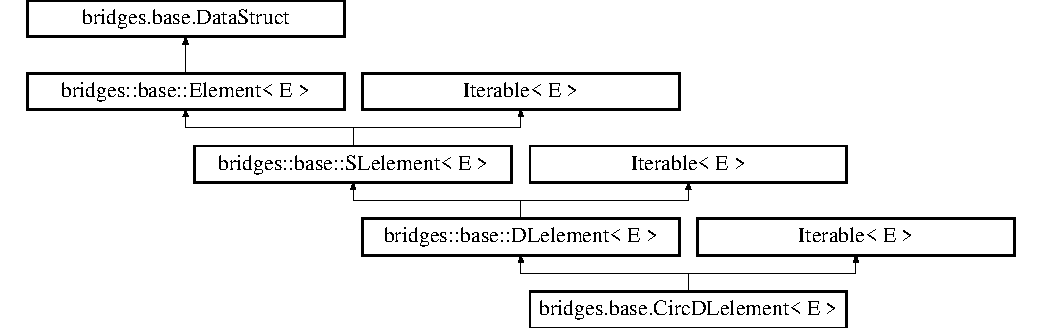
\includegraphics[height=5.000000cm]{classbridges_1_1base_1_1_circ_d_lelement}
\end{center}
\end{figure}


\subsection{Detailed Description}
This class can be used to instantiate Circular Doubly Linked List Elements. 

Structurally they are the same as doubly linked elements except that each node constructed with the next and the previous pointers points to itself.

User\textquotesingle{}s implementation of the circularly linked list needs to ensure that the last node\textquotesingle{}s next pointer points to the first node and the first node\textquotesingle{}s previous pointer points to the last node, as the visualization generation is dependent on this.

Elements have labels (string) that are displayed on the visualization. Elements take an generic object E as a user defined parameter, which can be any native type or object.

Elements contain a visualizer (\hyperlink{classbridges_1_1base_1_1_element_visualizer}{Element\+Visualizer}) object for setting visual attributes (color, shape, opacity, size), necessary for displaying them in a web browser.

Elements also have a \hyperlink{classbridges_1_1base_1_1_link_visualizer}{Link\+Visualizer} object that is used when they are linked to another element, appropriate for setting link attributes, between the element and its previous or next nodes.

\begin{DoxySeeAlso}{See also}
Example Tutorial at \href{http://bridgesuncc.github.io/tutorials/CircularDoublyLinkedList.html}{\tt http\+://bridgesuncc.\+github.\+io/tutorials/\+Circular\+Doubly\+Linked\+List.\+html}
\end{DoxySeeAlso}
\begin{DoxyAuthor}{Author}
Kalpathi Subramanian
\end{DoxyAuthor}
\begin{DoxyDate}{Date}
7/17/16, 1/16/17, 7/14/19
\end{DoxyDate}

\begin{DoxyParams}{Parameters}
{\em E} & the generic parameter object that contains application specific data, defined by the user when instantiating this object. \\
\hline
\end{DoxyParams}
\subsection*{Public Member Functions}
\begin{DoxyCompactItemize}
\item 
\hyperlink{classbridges_1_1base_1_1_circ_d_lelement_ad14ccb772d52c36802c118f2b3f15d59}{Circ\+D\+Lelement} ()
\item 
\hyperlink{classbridges_1_1base_1_1_circ_d_lelement_a84b2ebf47d2ca24077a800b240d8d157}{Circ\+D\+Lelement} (String label, E e)
\item 
\hyperlink{classbridges_1_1base_1_1_circ_d_lelement_a98a471fc3225ed80595e1ffdb377e336}{Circ\+D\+Lelement} (\hyperlink{classbridges_1_1base_1_1_circ_d_lelement}{Circ\+D\+Lelement}$<$ E $>$ \hyperlink{classbridges_1_1base_1_1_s_lelement_abf61c96a74ad319d561c6952ea388e0e}{next}, \hyperlink{classbridges_1_1base_1_1_circ_d_lelement}{Circ\+D\+Lelement}$<$ E $>$ \hyperlink{classbridges_1_1base_1_1_d_lelement_a6eba4876f820b75ac6bde01d7dea9da7}{prev})
\item 
\hyperlink{classbridges_1_1base_1_1_circ_d_lelement_a86e04c826251be9a1a92c4649844e5e7}{Circ\+D\+Lelement} (E e, \hyperlink{classbridges_1_1base_1_1_circ_d_lelement}{Circ\+D\+Lelement}$<$ E $>$ \hyperlink{classbridges_1_1base_1_1_s_lelement_abf61c96a74ad319d561c6952ea388e0e}{next}, \hyperlink{classbridges_1_1base_1_1_circ_d_lelement}{Circ\+D\+Lelement}$<$ E $>$ \hyperlink{classbridges_1_1base_1_1_d_lelement_a6eba4876f820b75ac6bde01d7dea9da7}{prev})
\item 
String \hyperlink{classbridges_1_1base_1_1_circ_d_lelement_ab4885ae7517f1dd04874270c1c3eaf44}{get\+Data\+Struct\+Type} ()
\item 
\hyperlink{classbridges_1_1base_1_1_circ_d_lelement}{Circ\+D\+Lelement}$<$ E $>$ \hyperlink{classbridges_1_1base_1_1_circ_d_lelement_a9ace56dde1f4c23e9a8798c045100ee6}{get\+Next} ()
\item 
\hyperlink{classbridges_1_1base_1_1_circ_d_lelement}{Circ\+D\+Lelement}$<$ E $>$ \hyperlink{classbridges_1_1base_1_1_circ_d_lelement_aa2b83017a571694460f77dd31b4188ed}{get\+Prev} ()
\end{DoxyCompactItemize}
\subsection*{Additional Inherited Members}


\subsection{Constructor \& Destructor Documentation}
\mbox{\Hypertarget{classbridges_1_1base_1_1_circ_d_lelement_ad14ccb772d52c36802c118f2b3f15d59}\label{classbridges_1_1base_1_1_circ_d_lelement_ad14ccb772d52c36802c118f2b3f15d59}} 
\index{bridges\+::base\+::\+Circ\+D\+Lelement@{bridges\+::base\+::\+Circ\+D\+Lelement}!Circ\+D\+Lelement@{Circ\+D\+Lelement}}
\index{Circ\+D\+Lelement@{Circ\+D\+Lelement}!bridges\+::base\+::\+Circ\+D\+Lelement@{bridges\+::base\+::\+Circ\+D\+Lelement}}
\subsubsection{\texorpdfstring{Circ\+D\+Lelement()}{CircDLelement()}\hspace{0.1cm}{\footnotesize\ttfamily [1/4]}}
{\footnotesize\ttfamily \hyperlink{classbridges_1_1base_1_1_circ_d_lelement}{bridges.\+base.\+Circ\+D\+Lelement}$<$ E $>$.\hyperlink{classbridges_1_1base_1_1_circ_d_lelement}{Circ\+D\+Lelement} (\begin{DoxyParamCaption}{ }\end{DoxyParamCaption})}

Constructs an empty \hyperlink{classbridges_1_1base_1_1_circ_d_lelement}{Circ\+D\+Lelement} with next and prev pointers set to itself \mbox{\Hypertarget{classbridges_1_1base_1_1_circ_d_lelement_a84b2ebf47d2ca24077a800b240d8d157}\label{classbridges_1_1base_1_1_circ_d_lelement_a84b2ebf47d2ca24077a800b240d8d157}} 
\index{bridges\+::base\+::\+Circ\+D\+Lelement@{bridges\+::base\+::\+Circ\+D\+Lelement}!Circ\+D\+Lelement@{Circ\+D\+Lelement}}
\index{Circ\+D\+Lelement@{Circ\+D\+Lelement}!bridges\+::base\+::\+Circ\+D\+Lelement@{bridges\+::base\+::\+Circ\+D\+Lelement}}
\subsubsection{\texorpdfstring{Circ\+D\+Lelement()}{CircDLelement()}\hspace{0.1cm}{\footnotesize\ttfamily [2/4]}}
{\footnotesize\ttfamily \hyperlink{classbridges_1_1base_1_1_circ_d_lelement}{bridges.\+base.\+Circ\+D\+Lelement}$<$ E $>$.\hyperlink{classbridges_1_1base_1_1_circ_d_lelement}{Circ\+D\+Lelement} (\begin{DoxyParamCaption}\item[{String}]{label,  }\item[{E}]{e }\end{DoxyParamCaption})}

Constructs a \hyperlink{classbridges_1_1base_1_1_circ_d_lelement}{Circ\+D\+Lelement} labeled \char`\"{}label\char`\"{}, holding an object \char`\"{}e\char`\"{}, with next and prev pointers set to itself


\begin{DoxyParams}{Parameters}
{\em label} & the label for this \hyperlink{classbridges_1_1base_1_1_circ_d_lelement}{Circ\+D\+Lelement} that shows up on the Bridges visualization \\
\hline
{\em e} & the genereic object that this \hyperlink{classbridges_1_1base_1_1_circ_d_lelement}{Circ\+D\+Lelement} is holding \\
\hline
\end{DoxyParams}
\mbox{\Hypertarget{classbridges_1_1base_1_1_circ_d_lelement_a98a471fc3225ed80595e1ffdb377e336}\label{classbridges_1_1base_1_1_circ_d_lelement_a98a471fc3225ed80595e1ffdb377e336}} 
\index{bridges\+::base\+::\+Circ\+D\+Lelement@{bridges\+::base\+::\+Circ\+D\+Lelement}!Circ\+D\+Lelement@{Circ\+D\+Lelement}}
\index{Circ\+D\+Lelement@{Circ\+D\+Lelement}!bridges\+::base\+::\+Circ\+D\+Lelement@{bridges\+::base\+::\+Circ\+D\+Lelement}}
\subsubsection{\texorpdfstring{Circ\+D\+Lelement()}{CircDLelement()}\hspace{0.1cm}{\footnotesize\ttfamily [3/4]}}
{\footnotesize\ttfamily \hyperlink{classbridges_1_1base_1_1_circ_d_lelement}{bridges.\+base.\+Circ\+D\+Lelement}$<$ E $>$.\hyperlink{classbridges_1_1base_1_1_circ_d_lelement}{Circ\+D\+Lelement} (\begin{DoxyParamCaption}\item[{\hyperlink{classbridges_1_1base_1_1_circ_d_lelement}{Circ\+D\+Lelement}$<$ E $>$}]{next,  }\item[{\hyperlink{classbridges_1_1base_1_1_circ_d_lelement}{Circ\+D\+Lelement}$<$ E $>$}]{prev }\end{DoxyParamCaption})}

Constructs an empty \hyperlink{classbridges_1_1base_1_1_d_lelement}{D\+Lelement} with the next pointer set to the \hyperlink{classbridges_1_1base_1_1_circ_d_lelement}{Circ\+D\+Lelement} \char`\"{}next\char`\"{} and the prev pointer set to \hyperlink{classbridges_1_1base_1_1_circ_d_lelement}{Circ\+D\+Lelement} \char`\"{}prev\char`\"{}.


\begin{DoxyParams}{Parameters}
{\em next} & the \hyperlink{classbridges_1_1base_1_1_d_lelement}{D\+Lelement} that should be assigned to the next pointer \\
\hline
{\em prev} & the \hyperlink{classbridges_1_1base_1_1_d_lelement}{D\+Lelement} that should be assigned to the prev pointer \\
\hline
\end{DoxyParams}
\mbox{\Hypertarget{classbridges_1_1base_1_1_circ_d_lelement_a86e04c826251be9a1a92c4649844e5e7}\label{classbridges_1_1base_1_1_circ_d_lelement_a86e04c826251be9a1a92c4649844e5e7}} 
\index{bridges\+::base\+::\+Circ\+D\+Lelement@{bridges\+::base\+::\+Circ\+D\+Lelement}!Circ\+D\+Lelement@{Circ\+D\+Lelement}}
\index{Circ\+D\+Lelement@{Circ\+D\+Lelement}!bridges\+::base\+::\+Circ\+D\+Lelement@{bridges\+::base\+::\+Circ\+D\+Lelement}}
\subsubsection{\texorpdfstring{Circ\+D\+Lelement()}{CircDLelement()}\hspace{0.1cm}{\footnotesize\ttfamily [4/4]}}
{\footnotesize\ttfamily \hyperlink{classbridges_1_1base_1_1_circ_d_lelement}{bridges.\+base.\+Circ\+D\+Lelement}$<$ E $>$.\hyperlink{classbridges_1_1base_1_1_circ_d_lelement}{Circ\+D\+Lelement} (\begin{DoxyParamCaption}\item[{E}]{e,  }\item[{\hyperlink{classbridges_1_1base_1_1_circ_d_lelement}{Circ\+D\+Lelement}$<$ E $>$}]{next,  }\item[{\hyperlink{classbridges_1_1base_1_1_circ_d_lelement}{Circ\+D\+Lelement}$<$ E $>$}]{prev }\end{DoxyParamCaption})}

Constructs a \hyperlink{classbridges_1_1base_1_1_d_lelement}{D\+Lelement} holding an object \char`\"{}e\char`\"{}, with the next pointer set to the \hyperlink{classbridges_1_1base_1_1_d_lelement}{D\+Lelement} \char`\"{}next\char`\"{} and the prev pointer set to \hyperlink{classbridges_1_1base_1_1_d_lelement}{D\+Lelement} \char`\"{}prev\char`\"{}.


\begin{DoxyParams}{Parameters}
{\em e} & the generic object that this \hyperlink{classbridges_1_1base_1_1_circ_d_lelement}{Circ\+D\+Lelement} is holding \\
\hline
{\em next} & the \hyperlink{classbridges_1_1base_1_1_circ_d_lelement}{Circ\+D\+Lelement} that should be assigned to the next pointer \\
\hline
{\em prev} & the \hyperlink{classbridges_1_1base_1_1_circ_d_lelement}{Circ\+D\+Lelement} that should be assigned to the prev pointer \\
\hline
\end{DoxyParams}


\subsection{Member Function Documentation}
\mbox{\Hypertarget{classbridges_1_1base_1_1_circ_d_lelement_ab4885ae7517f1dd04874270c1c3eaf44}\label{classbridges_1_1base_1_1_circ_d_lelement_ab4885ae7517f1dd04874270c1c3eaf44}} 
\index{bridges\+::base\+::\+Circ\+D\+Lelement@{bridges\+::base\+::\+Circ\+D\+Lelement}!get\+Data\+Struct\+Type@{get\+Data\+Struct\+Type}}
\index{get\+Data\+Struct\+Type@{get\+Data\+Struct\+Type}!bridges\+::base\+::\+Circ\+D\+Lelement@{bridges\+::base\+::\+Circ\+D\+Lelement}}
\subsubsection{\texorpdfstring{get\+Data\+Struct\+Type()}{getDataStructType()}}
{\footnotesize\ttfamily String \hyperlink{classbridges_1_1base_1_1_circ_d_lelement}{bridges.\+base.\+Circ\+D\+Lelement}$<$ E $>$.get\+Data\+Struct\+Type (\begin{DoxyParamCaption}{ }\end{DoxyParamCaption})}

This method gets the name of the data structure type

\begin{DoxyReturn}{Returns}
The date structure type as a string 
\end{DoxyReturn}
\mbox{\Hypertarget{classbridges_1_1base_1_1_circ_d_lelement_a9ace56dde1f4c23e9a8798c045100ee6}\label{classbridges_1_1base_1_1_circ_d_lelement_a9ace56dde1f4c23e9a8798c045100ee6}} 
\index{bridges\+::base\+::\+Circ\+D\+Lelement@{bridges\+::base\+::\+Circ\+D\+Lelement}!get\+Next@{get\+Next}}
\index{get\+Next@{get\+Next}!bridges\+::base\+::\+Circ\+D\+Lelement@{bridges\+::base\+::\+Circ\+D\+Lelement}}
\subsubsection{\texorpdfstring{get\+Next()}{getNext()}}
{\footnotesize\ttfamily \hyperlink{classbridges_1_1base_1_1_circ_d_lelement}{Circ\+D\+Lelement}$<$E$>$ \hyperlink{classbridges_1_1base_1_1_circ_d_lelement}{bridges.\+base.\+Circ\+D\+Lelement}$<$ E $>$.get\+Next (\begin{DoxyParamCaption}{ }\end{DoxyParamCaption})}

This method returns the pointer to the next \hyperlink{classbridges_1_1base_1_1_d_lelement}{D\+Lelement}

\begin{DoxyReturn}{Returns}
the \hyperlink{classbridges_1_1base_1_1_d_lelement}{D\+Lelement} assigned to the next pointer 
\end{DoxyReturn}
\mbox{\Hypertarget{classbridges_1_1base_1_1_circ_d_lelement_aa2b83017a571694460f77dd31b4188ed}\label{classbridges_1_1base_1_1_circ_d_lelement_aa2b83017a571694460f77dd31b4188ed}} 
\index{bridges\+::base\+::\+Circ\+D\+Lelement@{bridges\+::base\+::\+Circ\+D\+Lelement}!get\+Prev@{get\+Prev}}
\index{get\+Prev@{get\+Prev}!bridges\+::base\+::\+Circ\+D\+Lelement@{bridges\+::base\+::\+Circ\+D\+Lelement}}
\subsubsection{\texorpdfstring{get\+Prev()}{getPrev()}}
{\footnotesize\ttfamily \hyperlink{classbridges_1_1base_1_1_circ_d_lelement}{Circ\+D\+Lelement}$<$E$>$ \hyperlink{classbridges_1_1base_1_1_circ_d_lelement}{bridges.\+base.\+Circ\+D\+Lelement}$<$ E $>$.get\+Prev (\begin{DoxyParamCaption}{ }\end{DoxyParamCaption})}

This method returns the pointer to the previous \hyperlink{classbridges_1_1base_1_1_d_lelement}{D\+Lelement}

\begin{DoxyReturn}{Returns}
the \hyperlink{classbridges_1_1base_1_1_d_lelement}{D\+Lelement} assigned to the prev pointer 
\end{DoxyReturn}


The documentation for this class was generated from the following file\+:\begin{DoxyCompactItemize}
\item 
/home/erik/work/bridges/bridges-\/java/src/main/java/bridges/base/\hyperlink{_circ_d_lelement_8java}{Circ\+D\+Lelement.\+java}\end{DoxyCompactItemize}

\hypertarget{classbridges_1_1base_1_1_circle}{}\section{bridges.\+base.\+Circle Class Reference}
\label{classbridges_1_1base_1_1_circle}\index{bridges.\+base.\+Circle@{bridges.\+base.\+Circle}}
Inheritance diagram for bridges.\+base.\+Circle\+:\begin{figure}[H]
\begin{center}
\leavevmode
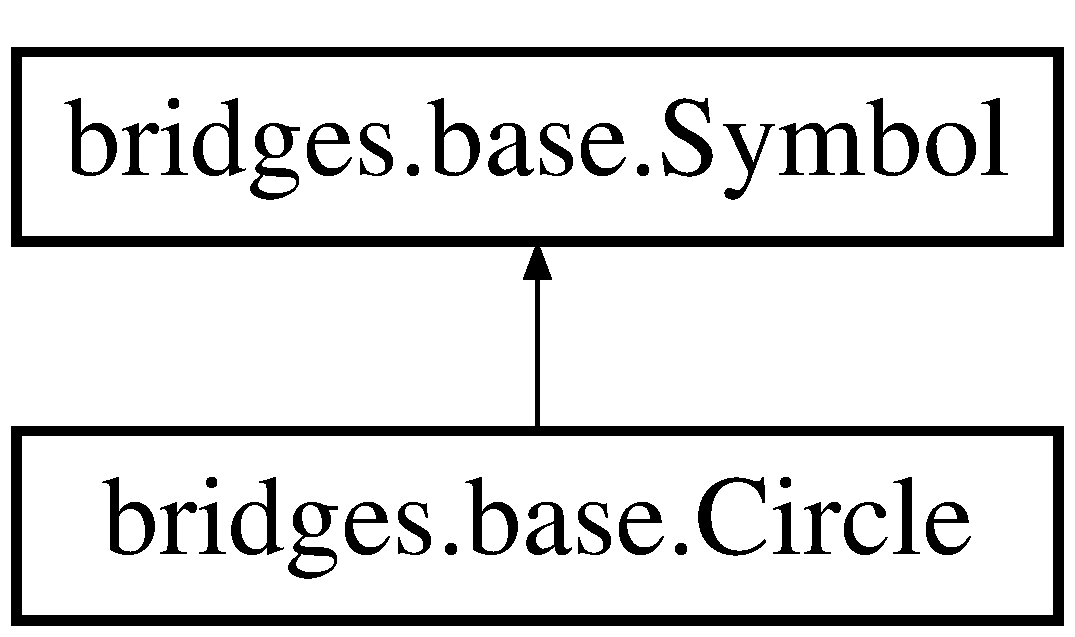
\includegraphics[height=2.000000cm]{classbridges_1_1base_1_1_circle}
\end{center}
\end{figure}


\subsection{Detailed Description}
This class defines a circle and is part of the symbol collection. A circle has a center and radius. 

Basic styling such as stroke and fill are defined in the superclass \hyperlink{classbridges_1_1base_1_1_symbol}{Symbol}.

\begin{DoxyAuthor}{Author}
Kalpathi Subramanian 
\end{DoxyAuthor}
\begin{DoxyDate}{Date}
12/24/18 
\end{DoxyDate}
\subsection*{Public Member Functions}
\begin{DoxyCompactItemize}
\item 
\hyperlink{classbridges_1_1base_1_1_circle_a807231dff01120041d7d209d049e3029}{Circle} ()
\item 
\hyperlink{classbridges_1_1base_1_1_circle_a32543e951646009960c1839b2b8e1a0a}{Circle} (float r)
\item 
\hyperlink{classbridges_1_1base_1_1_circle_a04460bea57f9ef4bd0a3d45e9a937096}{Circle} (float locx, float locy, float r)
\item 
String \hyperlink{classbridges_1_1base_1_1_circle_a3782ea68f0419747c00bd8b2bfa31462}{get\+Name} ()
\item 
void \hyperlink{classbridges_1_1base_1_1_circle_a38c9f2a569af42461323239ba90f559e}{set\+Radius} (float r)
\item 
void \hyperlink{classbridges_1_1base_1_1_circle_ac11cce75c482bb5c5751dfd1d5353b44}{set\+Circle} (float locx, float locy, float r)
\item 
void \hyperlink{classbridges_1_1base_1_1_circle_ad4e474d78a1aea48f947e76b96c93ccb}{translate} (float tx, float ty)
\item 
void \hyperlink{classbridges_1_1base_1_1_circle_acbb48177b6e99326294cd90f74b58a27}{scale} (float scale)
\item 
float \mbox{[}$\,$\mbox{]} \hyperlink{classbridges_1_1base_1_1_circle_a0752cc5f6e261ade3d27f34c1c566c80}{get\+Dimensions} ()
\item 
J\+S\+O\+N\+Object \hyperlink{classbridges_1_1base_1_1_circle_ad6a8b8e2dca562fd3fa5254ee861ed70}{get\+J\+S\+O\+N\+Representation} ()
\end{DoxyCompactItemize}
\subsection*{Additional Inherited Members}


\subsection{Constructor \& Destructor Documentation}
\mbox{\Hypertarget{classbridges_1_1base_1_1_circle_a807231dff01120041d7d209d049e3029}\label{classbridges_1_1base_1_1_circle_a807231dff01120041d7d209d049e3029}} 
\index{bridges\+::base\+::\+Circle@{bridges\+::base\+::\+Circle}!Circle@{Circle}}
\index{Circle@{Circle}!bridges\+::base\+::\+Circle@{bridges\+::base\+::\+Circle}}
\subsubsection{\texorpdfstring{Circle()}{Circle()}\hspace{0.1cm}{\footnotesize\ttfamily [1/3]}}
{\footnotesize\ttfamily bridges.\+base.\+Circle.\+Circle (\begin{DoxyParamCaption}{ }\end{DoxyParamCaption})}

Construct a default circle (center at origin, radius of 10 units) \mbox{\Hypertarget{classbridges_1_1base_1_1_circle_a32543e951646009960c1839b2b8e1a0a}\label{classbridges_1_1base_1_1_circle_a32543e951646009960c1839b2b8e1a0a}} 
\index{bridges\+::base\+::\+Circle@{bridges\+::base\+::\+Circle}!Circle@{Circle}}
\index{Circle@{Circle}!bridges\+::base\+::\+Circle@{bridges\+::base\+::\+Circle}}
\subsubsection{\texorpdfstring{Circle()}{Circle()}\hspace{0.1cm}{\footnotesize\ttfamily [2/3]}}
{\footnotesize\ttfamily bridges.\+base.\+Circle.\+Circle (\begin{DoxyParamCaption}\item[{float}]{r }\end{DoxyParamCaption})}

Construct a circle of radius r 
\begin{DoxyParams}{Parameters}
{\em r} & radius of circle \\
\hline
\end{DoxyParams}
\mbox{\Hypertarget{classbridges_1_1base_1_1_circle_a04460bea57f9ef4bd0a3d45e9a937096}\label{classbridges_1_1base_1_1_circle_a04460bea57f9ef4bd0a3d45e9a937096}} 
\index{bridges\+::base\+::\+Circle@{bridges\+::base\+::\+Circle}!Circle@{Circle}}
\index{Circle@{Circle}!bridges\+::base\+::\+Circle@{bridges\+::base\+::\+Circle}}
\subsubsection{\texorpdfstring{Circle()}{Circle()}\hspace{0.1cm}{\footnotesize\ttfamily [3/3]}}
{\footnotesize\ttfamily bridges.\+base.\+Circle.\+Circle (\begin{DoxyParamCaption}\item[{float}]{locx,  }\item[{float}]{locy,  }\item[{float}]{r }\end{DoxyParamCaption})}

Construct a circle with given location and radius 
\begin{DoxyParams}{Parameters}
{\em locx} & x coordinat of circle center \\
\hline
{\em locy} & y coordinat of circle center \\
\hline
{\em r} & radius of circle \\
\hline
\end{DoxyParams}


\subsection{Member Function Documentation}
\mbox{\Hypertarget{classbridges_1_1base_1_1_circle_a0752cc5f6e261ade3d27f34c1c566c80}\label{classbridges_1_1base_1_1_circle_a0752cc5f6e261ade3d27f34c1c566c80}} 
\index{bridges\+::base\+::\+Circle@{bridges\+::base\+::\+Circle}!get\+Dimensions@{get\+Dimensions}}
\index{get\+Dimensions@{get\+Dimensions}!bridges\+::base\+::\+Circle@{bridges\+::base\+::\+Circle}}
\subsubsection{\texorpdfstring{get\+Dimensions()}{getDimensions()}}
{\footnotesize\ttfamily float \mbox{[}$\,$\mbox{]} bridges.\+base.\+Circle.\+get\+Dimensions (\begin{DoxyParamCaption}{ }\end{DoxyParamCaption})}

This method returns the dimensions of the shape\+: min and max values in X and Y

\begin{DoxyReturn}{Returns}
array of 4 values This method returns the dimensions of the shape\+: min and max values in X and Y

bounding box of circle (array of 4 values) 
\end{DoxyReturn}
\mbox{\Hypertarget{classbridges_1_1base_1_1_circle_ad6a8b8e2dca562fd3fa5254ee861ed70}\label{classbridges_1_1base_1_1_circle_ad6a8b8e2dca562fd3fa5254ee861ed70}} 
\index{bridges\+::base\+::\+Circle@{bridges\+::base\+::\+Circle}!get\+J\+S\+O\+N\+Representation@{get\+J\+S\+O\+N\+Representation}}
\index{get\+J\+S\+O\+N\+Representation@{get\+J\+S\+O\+N\+Representation}!bridges\+::base\+::\+Circle@{bridges\+::base\+::\+Circle}}
\subsubsection{\texorpdfstring{get\+J\+S\+O\+N\+Representation()}{getJSONRepresentation()}}
{\footnotesize\ttfamily J\+S\+O\+N\+Object bridges.\+base.\+Circle.\+get\+J\+S\+O\+N\+Representation (\begin{DoxyParamCaption}{ }\end{DoxyParamCaption})}

This method returns the J\+S\+ON representation of the shape

\begin{DoxyReturn}{Returns}
J\+S\+ON representation of circle (string) 
\end{DoxyReturn}
\mbox{\Hypertarget{classbridges_1_1base_1_1_circle_a3782ea68f0419747c00bd8b2bfa31462}\label{classbridges_1_1base_1_1_circle_a3782ea68f0419747c00bd8b2bfa31462}} 
\index{bridges\+::base\+::\+Circle@{bridges\+::base\+::\+Circle}!get\+Name@{get\+Name}}
\index{get\+Name@{get\+Name}!bridges\+::base\+::\+Circle@{bridges\+::base\+::\+Circle}}
\subsubsection{\texorpdfstring{get\+Name()}{getName()}}
{\footnotesize\ttfamily String bridges.\+base.\+Circle.\+get\+Name (\begin{DoxyParamCaption}{ }\end{DoxyParamCaption})}

This method gets the name of the shape

\begin{DoxyReturn}{Returns}
name shape name 
\end{DoxyReturn}
\mbox{\Hypertarget{classbridges_1_1base_1_1_circle_acbb48177b6e99326294cd90f74b58a27}\label{classbridges_1_1base_1_1_circle_acbb48177b6e99326294cd90f74b58a27}} 
\index{bridges\+::base\+::\+Circle@{bridges\+::base\+::\+Circle}!scale@{scale}}
\index{scale@{scale}!bridges\+::base\+::\+Circle@{bridges\+::base\+::\+Circle}}
\subsubsection{\texorpdfstring{scale()}{scale()}}
{\footnotesize\ttfamily void bridges.\+base.\+Circle.\+scale (\begin{DoxyParamCaption}\item[{float}]{scale }\end{DoxyParamCaption})}

Scale the circle Only the radius needs to be scaled, using a single scale value


\begin{DoxyParams}{Parameters}
{\em scale} & factor s \\
\hline
\end{DoxyParams}
\mbox{\Hypertarget{classbridges_1_1base_1_1_circle_ac11cce75c482bb5c5751dfd1d5353b44}\label{classbridges_1_1base_1_1_circle_ac11cce75c482bb5c5751dfd1d5353b44}} 
\index{bridges\+::base\+::\+Circle@{bridges\+::base\+::\+Circle}!set\+Circle@{set\+Circle}}
\index{set\+Circle@{set\+Circle}!bridges\+::base\+::\+Circle@{bridges\+::base\+::\+Circle}}
\subsubsection{\texorpdfstring{set\+Circle()}{setCircle()}}
{\footnotesize\ttfamily void bridges.\+base.\+Circle.\+set\+Circle (\begin{DoxyParamCaption}\item[{float}]{locx,  }\item[{float}]{locy,  }\item[{float}]{r }\end{DoxyParamCaption})}

This method sets the circle dimensions


\begin{DoxyParams}{Parameters}
{\em locx} & x coordinate of circle center \\
\hline
{\em locy} & y coordinate of circle center \\
\hline
{\em r} & radius of circle \\
\hline
\end{DoxyParams}
\begin{DoxyReturn}{Returns}
none 
\end{DoxyReturn}
\mbox{\Hypertarget{classbridges_1_1base_1_1_circle_a38c9f2a569af42461323239ba90f559e}\label{classbridges_1_1base_1_1_circle_a38c9f2a569af42461323239ba90f559e}} 
\index{bridges\+::base\+::\+Circle@{bridges\+::base\+::\+Circle}!set\+Radius@{set\+Radius}}
\index{set\+Radius@{set\+Radius}!bridges\+::base\+::\+Circle@{bridges\+::base\+::\+Circle}}
\subsubsection{\texorpdfstring{set\+Radius()}{setRadius()}}
{\footnotesize\ttfamily void bridges.\+base.\+Circle.\+set\+Radius (\begin{DoxyParamCaption}\item[{float}]{r }\end{DoxyParamCaption})}

This method sets the radius of the circle


\begin{DoxyParams}{Parameters}
{\em r} & radius \\
\hline
\end{DoxyParams}
\mbox{\Hypertarget{classbridges_1_1base_1_1_circle_ad4e474d78a1aea48f947e76b96c93ccb}\label{classbridges_1_1base_1_1_circle_ad4e474d78a1aea48f947e76b96c93ccb}} 
\index{bridges\+::base\+::\+Circle@{bridges\+::base\+::\+Circle}!translate@{translate}}
\index{translate@{translate}!bridges\+::base\+::\+Circle@{bridges\+::base\+::\+Circle}}
\subsubsection{\texorpdfstring{translate()}{translate()}}
{\footnotesize\ttfamily void bridges.\+base.\+Circle.\+translate (\begin{DoxyParamCaption}\item[{float}]{tx,  }\item[{float}]{ty }\end{DoxyParamCaption})}

Translate the circle


\begin{DoxyParams}{Parameters}
{\em (tx,ty)} & translation vector \\
\hline
\end{DoxyParams}


The documentation for this class was generated from the following file\+:\begin{DoxyCompactItemize}
\item 
/home/erik/work/bridges/bridges-\/java/src/main/java/bridges/base/\hyperlink{_circle_8java}{Circle.\+java}\end{DoxyCompactItemize}

\hypertarget{classbridges_1_1base_1_1_circ_s_lelement}{}\section{bridges.\+base.\+Circ\+S\+Lelement$<$ E $>$ Class Template Reference}
\label{classbridges_1_1base_1_1_circ_s_lelement}\index{bridges.\+base.\+Circ\+S\+Lelement$<$ E $>$@{bridges.\+base.\+Circ\+S\+Lelement$<$ E $>$}}


This class can be used to instantiate Singly Linked Circular List Elements.  


Inheritance diagram for bridges.\+base.\+Circ\+S\+Lelement$<$ E $>$\+:\begin{figure}[H]
\begin{center}
\leavevmode
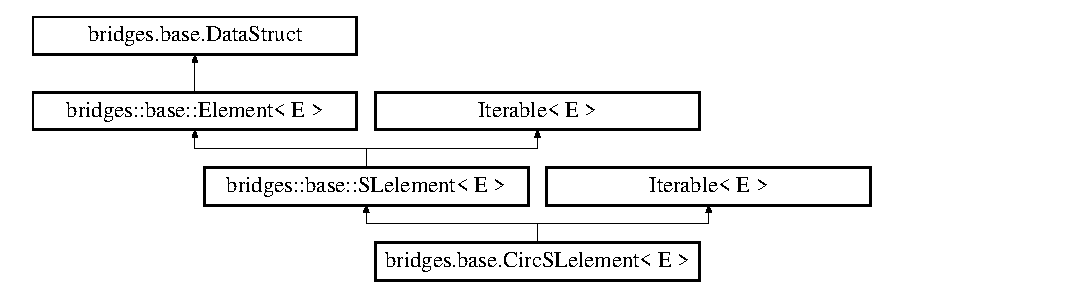
\includegraphics[height=4.000000cm]{classbridges_1_1base_1_1_circ_s_lelement}
\end{center}
\end{figure}
\subsection*{Public Member Functions}
\begin{DoxyCompactItemize}
\item 
\hyperlink{classbridges_1_1base_1_1_circ_s_lelement_a4a5a58cc7a0ec5170a828861c11df1b3}{Circ\+S\+Lelement} ()
\item 
\hyperlink{classbridges_1_1base_1_1_circ_s_lelement_a213d61713e51295d756669def911f080}{Circ\+S\+Lelement} (String label, E e)
\item 
\hyperlink{classbridges_1_1base_1_1_circ_s_lelement_ada65c593c8af7e6ed96fcdf12c26824f}{Circ\+S\+Lelement} (E e, \hyperlink{classbridges_1_1base_1_1_circ_s_lelement}{Circ\+S\+Lelement}$<$ E $>$ \hyperlink{classbridges_1_1base_1_1_s_lelement_abf61c96a74ad319d561c6952ea388e0e}{next})
\item 
\hyperlink{classbridges_1_1base_1_1_circ_s_lelement_ab9e5b98e8d917760b9651a52785358b9}{Circ\+S\+Lelement} (\hyperlink{classbridges_1_1base_1_1_circ_s_lelement}{Circ\+S\+Lelement}$<$ E $>$ \hyperlink{classbridges_1_1base_1_1_s_lelement_abf61c96a74ad319d561c6952ea388e0e}{next})
\item 
String \hyperlink{classbridges_1_1base_1_1_circ_s_lelement_ad56acddc52e8e0b6869a6f24f1e0a90e}{get\+Data\+Struct\+Type} ()
\item 
\hyperlink{classbridges_1_1base_1_1_circ_s_lelement}{Circ\+S\+Lelement}$<$ E $>$ \hyperlink{classbridges_1_1base_1_1_circ_s_lelement_ae18b07e3f1d37b5eca0cae22efc0d395}{get\+Next} ()
\item 
String \hyperlink{classbridges_1_1base_1_1_circ_s_lelement_af307188926766e73efb988f102ce9740}{to\+String} ()
\end{DoxyCompactItemize}
\subsection*{Additional Inherited Members}


\subsection{Detailed Description}
This class can be used to instantiate Singly Linked Circular List Elements. 

Structurally they are the same as singly linked elements except that each node constructed with the next point pointing to itself; User\textquotesingle{}s implementation of the circularly linked list needs to ensure that the last node points to first node of the list, as the visualization generation is dependent on this.

Elements have labels (string) that are displayed on the visualization. Elements take an generic object as a user defined parameter, E, which can be any native type or object.

Elements contains a visualizer (\hyperlink{classbridges_1_1base_1_1_element_visualizer}{Element\+Visualizer}) object for setting visual attributes (color, shape, opacity, size), necessary for displaying them in a web browser.

Elements also have a \hyperlink{classbridges_1_1base_1_1_link_visualizer}{Link\+Visualizer} object that is used when they are linked to another element, appropriate for setting link attributes, between an element and its next element.

\begin{DoxyAuthor}{Author}
Kalpathi Subramanian
\end{DoxyAuthor}
\begin{DoxyDate}{Date}
6/22/16, 1/7/17, 5/17/17
\end{DoxyDate}

\begin{DoxyParams}{Parameters}
{\em $<$\+E$>$} & the generic parameter that is defined by the application\\
\hline
\end{DoxyParams}
\begin{DoxySeeAlso}{See also}
Example Tutorial at ~\newline
 \href{http://bridgesuncc.github.io/Hello_World_Tutorials/CSLL.html}{\tt http\+://bridgesuncc.\+github.\+io/\+Hello\+\_\+\+World\+\_\+\+Tutorials/\+C\+S\+L\+L.\+html} 
\end{DoxySeeAlso}


\subsection{Constructor \& Destructor Documentation}
\hypertarget{classbridges_1_1base_1_1_circ_s_lelement_a4a5a58cc7a0ec5170a828861c11df1b3}{}\index{bridges\+::base\+::\+Circ\+S\+Lelement@{bridges\+::base\+::\+Circ\+S\+Lelement}!Circ\+S\+Lelement@{Circ\+S\+Lelement}}
\index{Circ\+S\+Lelement@{Circ\+S\+Lelement}!bridges\+::base\+::\+Circ\+S\+Lelement@{bridges\+::base\+::\+Circ\+S\+Lelement}}
\subsubsection[{Circ\+S\+Lelement()}]{\setlength{\rightskip}{0pt plus 5cm}{\bf bridges.\+base.\+Circ\+S\+Lelement}$<$ E $>$.{\bf Circ\+S\+Lelement} (
\begin{DoxyParamCaption}
{}
\end{DoxyParamCaption}
)}\label{classbridges_1_1base_1_1_circ_s_lelement_a4a5a58cc7a0ec5170a828861c11df1b3}
This constructor creates an \hyperlink{classbridges_1_1base_1_1_circ_s_lelement}{Circ\+S\+Lelement} object and sets its next pointer to itself \hypertarget{classbridges_1_1base_1_1_circ_s_lelement_a213d61713e51295d756669def911f080}{}\index{bridges\+::base\+::\+Circ\+S\+Lelement@{bridges\+::base\+::\+Circ\+S\+Lelement}!Circ\+S\+Lelement@{Circ\+S\+Lelement}}
\index{Circ\+S\+Lelement@{Circ\+S\+Lelement}!bridges\+::base\+::\+Circ\+S\+Lelement@{bridges\+::base\+::\+Circ\+S\+Lelement}}
\subsubsection[{Circ\+S\+Lelement(\+String label, E e)}]{\setlength{\rightskip}{0pt plus 5cm}{\bf bridges.\+base.\+Circ\+S\+Lelement}$<$ E $>$.{\bf Circ\+S\+Lelement} (
\begin{DoxyParamCaption}
\item[{String}]{label, }
\item[{E}]{e}
\end{DoxyParamCaption}
)}\label{classbridges_1_1base_1_1_circ_s_lelement_a213d61713e51295d756669def911f080}
This constructor creates an \hyperlink{classbridges_1_1base_1_1_circ_s_lelement}{Circ\+S\+Lelement} object of value \char`\"{}e\char`\"{} and label \char`\"{}label\char`\"{} and sets the next pointer to null


\begin{DoxyParams}{Parameters}
{\em label} & the label of \hyperlink{classbridges_1_1base_1_1_circ_s_lelement}{Circ\+S\+Lelement} that shows up on the Bridges visualization \\
\hline
{\em e} & the generic object that this \hyperlink{classbridges_1_1base_1_1_circ_s_lelement}{Circ\+S\+Lelement} will hold \\
\hline
\end{DoxyParams}
\hypertarget{classbridges_1_1base_1_1_circ_s_lelement_ada65c593c8af7e6ed96fcdf12c26824f}{}\index{bridges\+::base\+::\+Circ\+S\+Lelement@{bridges\+::base\+::\+Circ\+S\+Lelement}!Circ\+S\+Lelement@{Circ\+S\+Lelement}}
\index{Circ\+S\+Lelement@{Circ\+S\+Lelement}!bridges\+::base\+::\+Circ\+S\+Lelement@{bridges\+::base\+::\+Circ\+S\+Lelement}}
\subsubsection[{Circ\+S\+Lelement(\+E e, Circ\+S\+Lelement$<$ E $>$ next)}]{\setlength{\rightskip}{0pt plus 5cm}{\bf bridges.\+base.\+Circ\+S\+Lelement}$<$ E $>$.{\bf Circ\+S\+Lelement} (
\begin{DoxyParamCaption}
\item[{E}]{e, }
\item[{{\bf Circ\+S\+Lelement}$<$ E $>$}]{next}
\end{DoxyParamCaption}
)}\label{classbridges_1_1base_1_1_circ_s_lelement_ada65c593c8af7e6ed96fcdf12c26824f}
Creates a new element with value \char`\"{}e\char`\"{} and sets the next pointer to the \hyperlink{classbridges_1_1base_1_1_circ_s_lelement}{Circ\+S\+Lelement} referenced by the \char`\"{}next\char`\"{} argument


\begin{DoxyParams}{Parameters}
{\em e} & the generic object that this \hyperlink{classbridges_1_1base_1_1_circ_s_lelement}{Circ\+S\+Lelement} will hold \\
\hline
{\em next} & the \hyperlink{classbridges_1_1base_1_1_circ_s_lelement}{Circ\+S\+Lelement} that should be assigned to the next pointer \\
\hline
\end{DoxyParams}
\hypertarget{classbridges_1_1base_1_1_circ_s_lelement_ab9e5b98e8d917760b9651a52785358b9}{}\index{bridges\+::base\+::\+Circ\+S\+Lelement@{bridges\+::base\+::\+Circ\+S\+Lelement}!Circ\+S\+Lelement@{Circ\+S\+Lelement}}
\index{Circ\+S\+Lelement@{Circ\+S\+Lelement}!bridges\+::base\+::\+Circ\+S\+Lelement@{bridges\+::base\+::\+Circ\+S\+Lelement}}
\subsubsection[{Circ\+S\+Lelement(\+Circ\+S\+Lelement$<$ E $>$ next)}]{\setlength{\rightskip}{0pt plus 5cm}{\bf bridges.\+base.\+Circ\+S\+Lelement}$<$ E $>$.{\bf Circ\+S\+Lelement} (
\begin{DoxyParamCaption}
\item[{{\bf Circ\+S\+Lelement}$<$ E $>$}]{next}
\end{DoxyParamCaption}
)}\label{classbridges_1_1base_1_1_circ_s_lelement_ab9e5b98e8d917760b9651a52785358b9}
Creates a new element and sets the next pointer to the \hyperlink{classbridges_1_1base_1_1_circ_s_lelement}{Circ\+S\+Lelement} \char`\"{}next\char`\"{}


\begin{DoxyParams}{Parameters}
{\em next} & the \hyperlink{classbridges_1_1base_1_1_circ_s_lelement}{Circ\+S\+Lelement} that should be assigned to the next pointer \\
\hline
\end{DoxyParams}


\subsection{Member Function Documentation}
\hypertarget{classbridges_1_1base_1_1_circ_s_lelement_ad56acddc52e8e0b6869a6f24f1e0a90e}{}\index{bridges\+::base\+::\+Circ\+S\+Lelement@{bridges\+::base\+::\+Circ\+S\+Lelement}!get\+Data\+Struct\+Type@{get\+Data\+Struct\+Type}}
\index{get\+Data\+Struct\+Type@{get\+Data\+Struct\+Type}!bridges\+::base\+::\+Circ\+S\+Lelement@{bridges\+::base\+::\+Circ\+S\+Lelement}}
\subsubsection[{get\+Data\+Struct\+Type()}]{\setlength{\rightskip}{0pt plus 5cm}String {\bf bridges.\+base.\+Circ\+S\+Lelement}$<$ E $>$.get\+Data\+Struct\+Type (
\begin{DoxyParamCaption}
{}
\end{DoxyParamCaption}
)}\label{classbridges_1_1base_1_1_circ_s_lelement_ad56acddc52e8e0b6869a6f24f1e0a90e}
This method gets the data structure type

\begin{DoxyReturn}{Returns}
The date structure type as a string 
\end{DoxyReturn}
\hypertarget{classbridges_1_1base_1_1_circ_s_lelement_ae18b07e3f1d37b5eca0cae22efc0d395}{}\index{bridges\+::base\+::\+Circ\+S\+Lelement@{bridges\+::base\+::\+Circ\+S\+Lelement}!get\+Next@{get\+Next}}
\index{get\+Next@{get\+Next}!bridges\+::base\+::\+Circ\+S\+Lelement@{bridges\+::base\+::\+Circ\+S\+Lelement}}
\subsubsection[{get\+Next()}]{\setlength{\rightskip}{0pt plus 5cm}{\bf Circ\+S\+Lelement}$<$E$>$ {\bf bridges.\+base.\+Circ\+S\+Lelement}$<$ E $>$.get\+Next (
\begin{DoxyParamCaption}
{}
\end{DoxyParamCaption}
)}\label{classbridges_1_1base_1_1_circ_s_lelement_ae18b07e3f1d37b5eca0cae22efc0d395}
Retrieves the next \hyperlink{classbridges_1_1base_1_1_circ_s_lelement}{Circ\+S\+Lelement}

\begin{DoxyReturn}{Returns}
Circ\+S\+Lelement$<$\+E$>$ assigned to next 
\end{DoxyReturn}
\hypertarget{classbridges_1_1base_1_1_circ_s_lelement_af307188926766e73efb988f102ce9740}{}\index{bridges\+::base\+::\+Circ\+S\+Lelement@{bridges\+::base\+::\+Circ\+S\+Lelement}!to\+String@{to\+String}}
\index{to\+String@{to\+String}!bridges\+::base\+::\+Circ\+S\+Lelement@{bridges\+::base\+::\+Circ\+S\+Lelement}}
\subsubsection[{to\+String()}]{\setlength{\rightskip}{0pt plus 5cm}String {\bf bridges.\+base.\+Circ\+S\+Lelement}$<$ E $>$.to\+String (
\begin{DoxyParamCaption}
{}
\end{DoxyParamCaption}
)}\label{classbridges_1_1base_1_1_circ_s_lelement_af307188926766e73efb988f102ce9740}
(non-\/\+Javadoc)

\begin{DoxySeeAlso}{See also}
java.\+lang.\+Object\+::to\+String() 
\end{DoxySeeAlso}


The documentation for this class was generated from the following file\+:\begin{DoxyCompactItemize}
\item 
/\+Users/krs/gr/bridges/client/java/src/main/java/bridges/base/\hyperlink{_circ_s_lelement_8java}{Circ\+S\+Lelement.\+java}\end{DoxyCompactItemize}

\hypertarget{classbridges_1_1base_1_1_color}{}\section{bridges.\+base.\+Color Class Reference}
\label{classbridges_1_1base_1_1_color}\index{bridges.\+base.\+Color@{bridges.\+base.\+Color}}


This class is used to represent colors in B\+R\+I\+D\+G\+ES.  


\subsection*{Public Member Functions}
\begin{DoxyCompactItemize}
\item 
\mbox{\hyperlink{classbridges_1_1base_1_1_color_ab6d71ac2ee1430fb2db2fbe34e692de8}{Color}} ()
\item 
\mbox{\hyperlink{classbridges_1_1base_1_1_color_a15f56590ca3c9cc161c7bfa47060ad21}{Color}} (int r, int g, int b, float a)
\item 
\mbox{\hyperlink{classbridges_1_1base_1_1_color_a5fab564fa4eec8bece64f847ebd42948}{Color}} (int r, int g, int b)
\item 
\mbox{\hyperlink{classbridges_1_1base_1_1_color_a5cb17fdf8eddf44fc0763ceb7d4d833b}{Color}} (String color)
\item 
void \mbox{\hyperlink{classbridges_1_1base_1_1_color_a5559b1c7eb4c3901526b1012029b528f}{set\+Color}} (int r, int g, int b, float a)
\item 
void \mbox{\hyperlink{classbridges_1_1base_1_1_color_a1d78967703924b709e76def5b2b3ee9a}{set\+Red}} (int r)
\item 
int \mbox{\hyperlink{classbridges_1_1base_1_1_color_af1a30dc925b35d6bfe609f8838651025}{get\+Red}} ()
\item 
void \mbox{\hyperlink{classbridges_1_1base_1_1_color_a415a28133ade4e216c02ecdfc8a32a1d}{set\+Green}} (int g)
\item 
int \mbox{\hyperlink{classbridges_1_1base_1_1_color_a8f3fdd23cf785704faa2e3701e25978f}{get\+Green}} ()
\item 
void \mbox{\hyperlink{classbridges_1_1base_1_1_color_a0e04156b1573cf8002c4d9cb69825657}{set\+Blue}} (int b)
\item 
int \mbox{\hyperlink{classbridges_1_1base_1_1_color_ad4b82e1eb9ff59857d2868edd8d4ce65}{get\+Blue}} ()
\item 
void \mbox{\hyperlink{classbridges_1_1base_1_1_color_afab07ce64efa1fa5797795670b0effb6}{set\+Alpha}} (float a)
\item 
float \mbox{\hyperlink{classbridges_1_1base_1_1_color_a7c4247e31ecd8fcc61ef208d5deefe68}{get\+Alpha}} ()
\item 
String \mbox{\hyperlink{classbridges_1_1base_1_1_color_a2f9b0cb588e49b2ebf2f015d4d7507d0}{get\+Representation}} ()
\item 
String \mbox{\hyperlink{classbridges_1_1base_1_1_color_aced9bc89248b85686ba5385472974fe6}{get\+Hex\+Representation}} ()
\item 
byte \mbox{[}$\,$\mbox{]} \mbox{\hyperlink{classbridges_1_1base_1_1_color_a07215c888a6d17374a3d862ff30d5f93}{get\+Byte\+Representation}} ()
\item 
void \mbox{\hyperlink{classbridges_1_1base_1_1_color_a54dcd31227bde0f5d0a4f5d3b5a24ed2}{set\+Color}} (String col\+\_\+name)
\end{DoxyCompactItemize}


\subsection{Detailed Description}
This class is used to represent colors in B\+R\+I\+D\+G\+ES. 

We use an R\+G\+BA model to represent colors, with each component in the range 0-\/255. B\+R\+I\+D\+G\+ES also supports named colors for user convenience, but these are converted into \mbox{[}R\+G\+BA\mbox{]} prior to transmission to the server for visualization.

\begin{DoxyAuthor}{Author}
K.\+R. Subramanian, 
\end{DoxyAuthor}
\begin{DoxyDate}{Date}
7/14/16 
\end{DoxyDate}


\subsection{Constructor \& Destructor Documentation}
\mbox{\Hypertarget{classbridges_1_1base_1_1_color_ab6d71ac2ee1430fb2db2fbe34e692de8}\label{classbridges_1_1base_1_1_color_ab6d71ac2ee1430fb2db2fbe34e692de8}} 
\index{bridges\+::base\+::\+Color@{bridges\+::base\+::\+Color}!Color@{Color}}
\index{Color@{Color}!bridges\+::base\+::\+Color@{bridges\+::base\+::\+Color}}
\subsubsection{\texorpdfstring{Color()}{Color()}\hspace{0.1cm}{\footnotesize\ttfamily [1/4]}}
{\footnotesize\ttfamily bridges.\+base.\+Color.\+Color (\begin{DoxyParamCaption}{ }\end{DoxyParamCaption})}

Constructors \mbox{\Hypertarget{classbridges_1_1base_1_1_color_a15f56590ca3c9cc161c7bfa47060ad21}\label{classbridges_1_1base_1_1_color_a15f56590ca3c9cc161c7bfa47060ad21}} 
\index{bridges\+::base\+::\+Color@{bridges\+::base\+::\+Color}!Color@{Color}}
\index{Color@{Color}!bridges\+::base\+::\+Color@{bridges\+::base\+::\+Color}}
\subsubsection{\texorpdfstring{Color()}{Color()}\hspace{0.1cm}{\footnotesize\ttfamily [2/4]}}
{\footnotesize\ttfamily bridges.\+base.\+Color.\+Color (\begin{DoxyParamCaption}\item[{int}]{r,  }\item[{int}]{g,  }\item[{int}]{b,  }\item[{float}]{a }\end{DoxyParamCaption})}

Constructor, given r, g, b, a components


\begin{DoxyParams}{Parameters}
{\em r,g,b,a} & -\/ checked to be in the range 0-\/255 \\
\hline
\end{DoxyParams}
\mbox{\Hypertarget{classbridges_1_1base_1_1_color_a5fab564fa4eec8bece64f847ebd42948}\label{classbridges_1_1base_1_1_color_a5fab564fa4eec8bece64f847ebd42948}} 
\index{bridges\+::base\+::\+Color@{bridges\+::base\+::\+Color}!Color@{Color}}
\index{Color@{Color}!bridges\+::base\+::\+Color@{bridges\+::base\+::\+Color}}
\subsubsection{\texorpdfstring{Color()}{Color()}\hspace{0.1cm}{\footnotesize\ttfamily [3/4]}}
{\footnotesize\ttfamily bridges.\+base.\+Color.\+Color (\begin{DoxyParamCaption}\item[{int}]{r,  }\item[{int}]{g,  }\item[{int}]{b }\end{DoxyParamCaption})}

Constructor, given r, g, b components alpha (opacity) defaults to 255


\begin{DoxyParams}{Parameters}
{\em r,g,b,a} & -\/ checked to be in the range 0-\/255 \\
\hline
\end{DoxyParams}
\mbox{\Hypertarget{classbridges_1_1base_1_1_color_a5cb17fdf8eddf44fc0763ceb7d4d833b}\label{classbridges_1_1base_1_1_color_a5cb17fdf8eddf44fc0763ceb7d4d833b}} 
\index{bridges\+::base\+::\+Color@{bridges\+::base\+::\+Color}!Color@{Color}}
\index{Color@{Color}!bridges\+::base\+::\+Color@{bridges\+::base\+::\+Color}}
\subsubsection{\texorpdfstring{Color()}{Color()}\hspace{0.1cm}{\footnotesize\ttfamily [4/4]}}
{\footnotesize\ttfamily bridges.\+base.\+Color.\+Color (\begin{DoxyParamCaption}\item[{String}]{color }\end{DoxyParamCaption})}

Constructor, given color name


\begin{DoxyParams}{Parameters}
{\em color} & -\/ checked to be in the list of possible color names \\
\hline
\end{DoxyParams}


\subsection{Member Function Documentation}
\mbox{\Hypertarget{classbridges_1_1base_1_1_color_a7c4247e31ecd8fcc61ef208d5deefe68}\label{classbridges_1_1base_1_1_color_a7c4247e31ecd8fcc61ef208d5deefe68}} 
\index{bridges\+::base\+::\+Color@{bridges\+::base\+::\+Color}!get\+Alpha@{get\+Alpha}}
\index{get\+Alpha@{get\+Alpha}!bridges\+::base\+::\+Color@{bridges\+::base\+::\+Color}}
\subsubsection{\texorpdfstring{get\+Alpha()}{getAlpha()}}
{\footnotesize\ttfamily float bridges.\+base.\+Color.\+get\+Alpha (\begin{DoxyParamCaption}{ }\end{DoxyParamCaption})}

gets the alpha component

\begin{DoxyReturn}{Returns}
alpha -\/ returns the alpha(opacity) component of the color 
\end{DoxyReturn}
\mbox{\Hypertarget{classbridges_1_1base_1_1_color_ad4b82e1eb9ff59857d2868edd8d4ce65}\label{classbridges_1_1base_1_1_color_ad4b82e1eb9ff59857d2868edd8d4ce65}} 
\index{bridges\+::base\+::\+Color@{bridges\+::base\+::\+Color}!get\+Blue@{get\+Blue}}
\index{get\+Blue@{get\+Blue}!bridges\+::base\+::\+Color@{bridges\+::base\+::\+Color}}
\subsubsection{\texorpdfstring{get\+Blue()}{getBlue()}}
{\footnotesize\ttfamily int bridges.\+base.\+Color.\+get\+Blue (\begin{DoxyParamCaption}{ }\end{DoxyParamCaption})}

gets the blue component

\begin{DoxyReturn}{Returns}
blue -\/ returns the blue component of the color 
\end{DoxyReturn}
\mbox{\Hypertarget{classbridges_1_1base_1_1_color_a07215c888a6d17374a3d862ff30d5f93}\label{classbridges_1_1base_1_1_color_a07215c888a6d17374a3d862ff30d5f93}} 
\index{bridges\+::base\+::\+Color@{bridges\+::base\+::\+Color}!get\+Byte\+Representation@{get\+Byte\+Representation}}
\index{get\+Byte\+Representation@{get\+Byte\+Representation}!bridges\+::base\+::\+Color@{bridges\+::base\+::\+Color}}
\subsubsection{\texorpdfstring{get\+Byte\+Representation()}{getByteRepresentation()}}
{\footnotesize\ttfamily byte \mbox{[}$\,$\mbox{]} bridges.\+base.\+Color.\+get\+Byte\+Representation (\begin{DoxyParamCaption}{ }\end{DoxyParamCaption})}

gets a Byte array representation of a \mbox{\hyperlink{classbridges_1_1base_1_1_color}{Color}}

\begin{DoxyReturn}{Returns}
-\/ returns the R\+G\+BA color as a byte array 
\end{DoxyReturn}
\mbox{\Hypertarget{classbridges_1_1base_1_1_color_a8f3fdd23cf785704faa2e3701e25978f}\label{classbridges_1_1base_1_1_color_a8f3fdd23cf785704faa2e3701e25978f}} 
\index{bridges\+::base\+::\+Color@{bridges\+::base\+::\+Color}!get\+Green@{get\+Green}}
\index{get\+Green@{get\+Green}!bridges\+::base\+::\+Color@{bridges\+::base\+::\+Color}}
\subsubsection{\texorpdfstring{get\+Green()}{getGreen()}}
{\footnotesize\ttfamily int bridges.\+base.\+Color.\+get\+Green (\begin{DoxyParamCaption}{ }\end{DoxyParamCaption})}

gets the green component

\begin{DoxyReturn}{Returns}
green -\/ returns the green component of the color 
\end{DoxyReturn}
\mbox{\Hypertarget{classbridges_1_1base_1_1_color_aced9bc89248b85686ba5385472974fe6}\label{classbridges_1_1base_1_1_color_aced9bc89248b85686ba5385472974fe6}} 
\index{bridges\+::base\+::\+Color@{bridges\+::base\+::\+Color}!get\+Hex\+Representation@{get\+Hex\+Representation}}
\index{get\+Hex\+Representation@{get\+Hex\+Representation}!bridges\+::base\+::\+Color@{bridges\+::base\+::\+Color}}
\subsubsection{\texorpdfstring{get\+Hex\+Representation()}{getHexRepresentation()}}
{\footnotesize\ttfamily String bridges.\+base.\+Color.\+get\+Hex\+Representation (\begin{DoxyParamCaption}{ }\end{DoxyParamCaption})}

gets the R\+GB \mbox{\hyperlink{classbridges_1_1base_1_1_color}{Color}} representation as a Hex String

\begin{DoxyReturn}{Returns}
-\/ returns the R\+GB color as hexadecimal String 
\end{DoxyReturn}
\mbox{\Hypertarget{classbridges_1_1base_1_1_color_af1a30dc925b35d6bfe609f8838651025}\label{classbridges_1_1base_1_1_color_af1a30dc925b35d6bfe609f8838651025}} 
\index{bridges\+::base\+::\+Color@{bridges\+::base\+::\+Color}!get\+Red@{get\+Red}}
\index{get\+Red@{get\+Red}!bridges\+::base\+::\+Color@{bridges\+::base\+::\+Color}}
\subsubsection{\texorpdfstring{get\+Red()}{getRed()}}
{\footnotesize\ttfamily int bridges.\+base.\+Color.\+get\+Red (\begin{DoxyParamCaption}{ }\end{DoxyParamCaption})}

gets the red component

\begin{DoxyReturn}{Returns}
red -\/ returns the red component of the color 
\end{DoxyReturn}
\mbox{\Hypertarget{classbridges_1_1base_1_1_color_a2f9b0cb588e49b2ebf2f015d4d7507d0}\label{classbridges_1_1base_1_1_color_a2f9b0cb588e49b2ebf2f015d4d7507d0}} 
\index{bridges\+::base\+::\+Color@{bridges\+::base\+::\+Color}!get\+Representation@{get\+Representation}}
\index{get\+Representation@{get\+Representation}!bridges\+::base\+::\+Color@{bridges\+::base\+::\+Color}}
\subsubsection{\texorpdfstring{get\+Representation()}{getRepresentation()}}
{\footnotesize\ttfamily String bridges.\+base.\+Color.\+get\+Representation (\begin{DoxyParamCaption}{ }\end{DoxyParamCaption})}

gets the \mbox{\hyperlink{classbridges_1_1base_1_1_color}{Color}} representation as a String

\begin{DoxyReturn}{Returns}
-\/ returns the color as a String with an R\+G\+BA array format 
\end{DoxyReturn}
\mbox{\Hypertarget{classbridges_1_1base_1_1_color_afab07ce64efa1fa5797795670b0effb6}\label{classbridges_1_1base_1_1_color_afab07ce64efa1fa5797795670b0effb6}} 
\index{bridges\+::base\+::\+Color@{bridges\+::base\+::\+Color}!set\+Alpha@{set\+Alpha}}
\index{set\+Alpha@{set\+Alpha}!bridges\+::base\+::\+Color@{bridges\+::base\+::\+Color}}
\subsubsection{\texorpdfstring{set\+Alpha()}{setAlpha()}}
{\footnotesize\ttfamily void bridges.\+base.\+Color.\+set\+Alpha (\begin{DoxyParamCaption}\item[{float}]{a }\end{DoxyParamCaption})}

sets the alpha(opacity) component


\begin{DoxyParams}{Parameters}
{\em a} & -\/ checked to be in the range 0-\/255 \\
\hline
\end{DoxyParams}
\mbox{\Hypertarget{classbridges_1_1base_1_1_color_a0e04156b1573cf8002c4d9cb69825657}\label{classbridges_1_1base_1_1_color_a0e04156b1573cf8002c4d9cb69825657}} 
\index{bridges\+::base\+::\+Color@{bridges\+::base\+::\+Color}!set\+Blue@{set\+Blue}}
\index{set\+Blue@{set\+Blue}!bridges\+::base\+::\+Color@{bridges\+::base\+::\+Color}}
\subsubsection{\texorpdfstring{set\+Blue()}{setBlue()}}
{\footnotesize\ttfamily void bridges.\+base.\+Color.\+set\+Blue (\begin{DoxyParamCaption}\item[{int}]{b }\end{DoxyParamCaption})}

sets the blue component


\begin{DoxyParams}{Parameters}
{\em b} & -\/ checked to be in the range 0-\/255 \\
\hline
\end{DoxyParams}
\mbox{\Hypertarget{classbridges_1_1base_1_1_color_a5559b1c7eb4c3901526b1012029b528f}\label{classbridges_1_1base_1_1_color_a5559b1c7eb4c3901526b1012029b528f}} 
\index{bridges\+::base\+::\+Color@{bridges\+::base\+::\+Color}!set\+Color@{set\+Color}}
\index{set\+Color@{set\+Color}!bridges\+::base\+::\+Color@{bridges\+::base\+::\+Color}}
\subsubsection{\texorpdfstring{set\+Color()}{setColor()}\hspace{0.1cm}{\footnotesize\ttfamily [1/2]}}
{\footnotesize\ttfamily void bridges.\+base.\+Color.\+set\+Color (\begin{DoxyParamCaption}\item[{int}]{r,  }\item[{int}]{g,  }\item[{int}]{b,  }\item[{float}]{a }\end{DoxyParamCaption})}

sets color to the given r, g, b, a components


\begin{DoxyParams}{Parameters}
{\em r,g,b,a} & -\/ checked to be in the range 0-\/255 \\
\hline
\end{DoxyParams}
\mbox{\Hypertarget{classbridges_1_1base_1_1_color_a54dcd31227bde0f5d0a4f5d3b5a24ed2}\label{classbridges_1_1base_1_1_color_a54dcd31227bde0f5d0a4f5d3b5a24ed2}} 
\index{bridges\+::base\+::\+Color@{bridges\+::base\+::\+Color}!set\+Color@{set\+Color}}
\index{set\+Color@{set\+Color}!bridges\+::base\+::\+Color@{bridges\+::base\+::\+Color}}
\subsubsection{\texorpdfstring{set\+Color()}{setColor()}\hspace{0.1cm}{\footnotesize\ttfamily [2/2]}}
{\footnotesize\ttfamily void bridges.\+base.\+Color.\+set\+Color (\begin{DoxyParamCaption}\item[{String}]{col\+\_\+name }\end{DoxyParamCaption})}

sets the color to the R\+G\+BA components given the color name


\begin{DoxyParams}{Parameters}
{\em col\+\_\+name} & color name \\
\hline
\end{DoxyParams}
\mbox{\Hypertarget{classbridges_1_1base_1_1_color_a415a28133ade4e216c02ecdfc8a32a1d}\label{classbridges_1_1base_1_1_color_a415a28133ade4e216c02ecdfc8a32a1d}} 
\index{bridges\+::base\+::\+Color@{bridges\+::base\+::\+Color}!set\+Green@{set\+Green}}
\index{set\+Green@{set\+Green}!bridges\+::base\+::\+Color@{bridges\+::base\+::\+Color}}
\subsubsection{\texorpdfstring{set\+Green()}{setGreen()}}
{\footnotesize\ttfamily void bridges.\+base.\+Color.\+set\+Green (\begin{DoxyParamCaption}\item[{int}]{g }\end{DoxyParamCaption})}

sets the green component


\begin{DoxyParams}{Parameters}
{\em g} & -\/ checked to be in the range 0-\/255 \\
\hline
\end{DoxyParams}
\mbox{\Hypertarget{classbridges_1_1base_1_1_color_a1d78967703924b709e76def5b2b3ee9a}\label{classbridges_1_1base_1_1_color_a1d78967703924b709e76def5b2b3ee9a}} 
\index{bridges\+::base\+::\+Color@{bridges\+::base\+::\+Color}!set\+Red@{set\+Red}}
\index{set\+Red@{set\+Red}!bridges\+::base\+::\+Color@{bridges\+::base\+::\+Color}}
\subsubsection{\texorpdfstring{set\+Red()}{setRed()}}
{\footnotesize\ttfamily void bridges.\+base.\+Color.\+set\+Red (\begin{DoxyParamCaption}\item[{int}]{r }\end{DoxyParamCaption})}

sets the red component


\begin{DoxyParams}{Parameters}
{\em r} & -\/ checked to be in the range 0-\/255 \\
\hline
\end{DoxyParams}


The documentation for this class was generated from the following file\+:\begin{DoxyCompactItemize}
\item 
/\+Users/kalpathi/gr/bridges/client/java/bridges-\/17/src/main/java/edu/uncc/cs/bridges\+\_\+v21/base/\mbox{\hyperlink{_color_8java}{Color.\+java}}\end{DoxyCompactItemize}

\hypertarget{classbridges_1_1base_1_1_color_grid}{}\doxysection{bridges.\+base.\+Color\+Grid Class Reference}
\label{classbridges_1_1base_1_1_color_grid}\index{bridges.base.ColorGrid@{bridges.base.ColorGrid}}
Inheritance diagram for bridges.\+base.\+Color\+Grid\+:\begin{figure}[H]
\begin{center}
\leavevmode
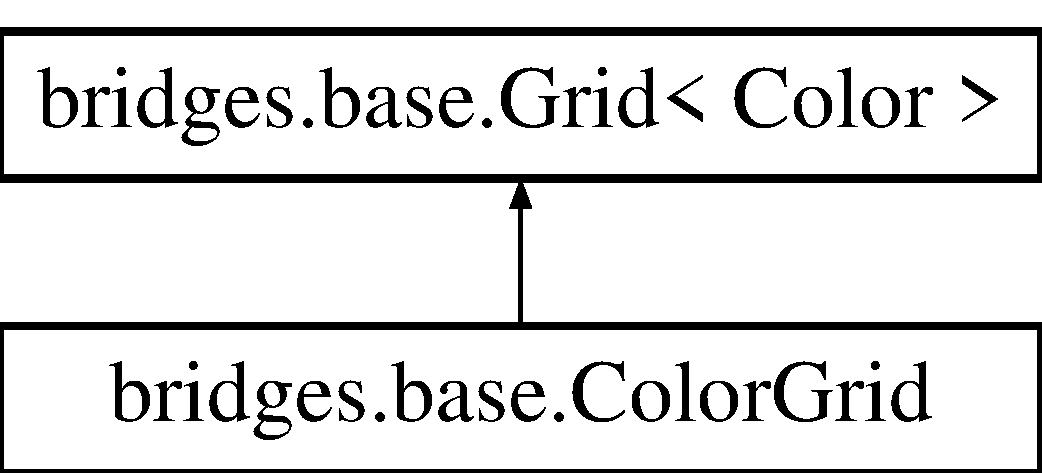
\includegraphics[height=2.000000cm]{classbridges_1_1base_1_1_color_grid}
\end{center}
\end{figure}


\doxysubsection{Detailed Description}
This is a class in B\+R\+I\+D\+G\+ES for representing an image. 

A \mbox{\hyperlink{classbridges_1_1base_1_1_color_grid}{Color\+Grid}} is essentially an image. One can construct an image of a particular size using the \mbox{\hyperlink{classbridges_1_1base_1_1_color_grid_af434a5a3dcbaf86e51ac6f9e1c1d7e5f}{Color\+Grid()}} constructor to be either blank or filled with a particular \mbox{\hyperlink{classbridges_1_1base_1_1_color}{Color}} depending on which constructor is called.

One can change the color of a pixel with \mbox{\hyperlink{classbridges_1_1base_1_1_grid_ab79ceb737423bb28ea2348e61a625a17}{set()}}. For instance, like that\+: 
\begin{DoxyCode}{0}
\DoxyCodeLine{\mbox{\hyperlink{classbridges_1_1base_1_1_color_grid_af434a5a3dcbaf86e51ac6f9e1c1d7e5f}{ColorGrid}} \mbox{\hyperlink{classbridges_1_1base_1_1_grid_ad1f3f6968d58188425bd992c05c655a6}{grid}} = \textcolor{keyword}{new} \mbox{\hyperlink{classbridges_1_1base_1_1_color_grid_af434a5a3dcbaf86e51ac6f9e1c1d7e5f}{ColorGrid}}(rows, columns);}
\DoxyCodeLine{\mbox{\hyperlink{classbridges_1_1base_1_1_grid_ad1f3f6968d58188425bd992c05c655a6}{grid}}.set (2, 3, \textcolor{keyword}{new} Color(\textcolor{stringliteral}{"lightsalmon"});}
\end{DoxyCode}


You can get a \mbox{\hyperlink{classbridges_1_1base_1_1_color_grid}{Color\+Grid}} from an existing Bridges \mbox{\hyperlink{classbridges_1_1base_1_1_color_grid}{Color\+Grid}} assignment using \mbox{\hyperlink{classbridges_1_1connect_1_1_data_source_a9556950d89b39ce61bead0879d1e2192}{bridges.\+connect.\+Data\+Source.\+get\+Color\+Grid\+From\+Assignment()}}

\begin{DoxySeeAlso}{See also}
There is a tutorial about \mbox{\hyperlink{classbridges_1_1base_1_1_color_grid}{Color\+Grid}} \+: \href{http://bridgesuncc.github.io/tutorials/Grid.html}{\texttt{ http\+://bridgesuncc.\+github.\+io/tutorials/\+Grid.\+html}}
\end{DoxySeeAlso}
\begin{DoxyAuthor}{Author}
David Burlinson, Erik Saule 
\end{DoxyAuthor}
\doxysubsection*{Public Member Functions}
\begin{DoxyCompactItemize}
\item 
String \mbox{\hyperlink{classbridges_1_1base_1_1_color_grid_a53a1f3f105f8545796f98e5fac559b5b}{get\+Data\+Struct\+Type}} ()
\item 
\mbox{\hyperlink{classbridges_1_1base_1_1_color_grid_af434a5a3dcbaf86e51ac6f9e1c1d7e5f}{Color\+Grid}} ()
\item 
\mbox{\hyperlink{classbridges_1_1base_1_1_color_grid_aafb4157a4c8129f30c1f989fcdfda544}{Color\+Grid}} (int rows, int cols)
\item 
\mbox{\hyperlink{classbridges_1_1base_1_1_color_grid_aef40242c93b66ab851e6afa64cada0b5}{Color\+Grid}} (int rows, int cols, \mbox{\hyperlink{classbridges_1_1base_1_1_color}{Color}} color)
\item 
int \mbox{\hyperlink{classbridges_1_1base_1_1_color_grid_a8793791e35f03b3e5a2e5ef3606ac124}{get\+Height}} ()
\item 
int \mbox{\hyperlink{classbridges_1_1base_1_1_color_grid_af872226de86ac8e8f2553fdc5bddc375}{get\+Width}} ()
\item 
String \mbox{\hyperlink{classbridges_1_1base_1_1_color_grid_a81ca0995d17b6cb31122b718dfa57286}{get\+Data\+Structure\+Representation}} ()
\end{DoxyCompactItemize}
\doxysubsection*{Additional Inherited Members}


\doxysubsection{Constructor \& Destructor Documentation}
\mbox{\Hypertarget{classbridges_1_1base_1_1_color_grid_af434a5a3dcbaf86e51ac6f9e1c1d7e5f}\label{classbridges_1_1base_1_1_color_grid_af434a5a3dcbaf86e51ac6f9e1c1d7e5f}} 
\index{bridges.base.ColorGrid@{bridges.base.ColorGrid}!ColorGrid@{ColorGrid}}
\index{ColorGrid@{ColorGrid}!bridges.base.ColorGrid@{bridges.base.ColorGrid}}
\doxysubsubsection{\texorpdfstring{ColorGrid()}{ColorGrid()}\hspace{0.1cm}{\footnotesize\ttfamily [1/3]}}
{\footnotesize\ttfamily bridges.\+base.\+Color\+Grid.\+Color\+Grid (\begin{DoxyParamCaption}{ }\end{DoxyParamCaption})}

Construct a color grid with defaulty sizes\+: \mbox{\Hypertarget{classbridges_1_1base_1_1_color_grid_aafb4157a4c8129f30c1f989fcdfda544}\label{classbridges_1_1base_1_1_color_grid_aafb4157a4c8129f30c1f989fcdfda544}} 
\index{bridges.base.ColorGrid@{bridges.base.ColorGrid}!ColorGrid@{ColorGrid}}
\index{ColorGrid@{ColorGrid}!bridges.base.ColorGrid@{bridges.base.ColorGrid}}
\doxysubsubsection{\texorpdfstring{ColorGrid()}{ColorGrid()}\hspace{0.1cm}{\footnotesize\ttfamily [2/3]}}
{\footnotesize\ttfamily bridges.\+base.\+Color\+Grid.\+Color\+Grid (\begin{DoxyParamCaption}\item[{int}]{rows,  }\item[{int}]{cols }\end{DoxyParamCaption})}

\mbox{\hyperlink{classbridges_1_1base_1_1_grid}{Grid}} constructor with size arguments


\begin{DoxyParams}{Parameters}
{\em rows} & -\/ int representing the number of rows of the grid \\
\hline
{\em cols} & -\/ int representing the number of columns of the grid \\
\hline
\end{DoxyParams}
\mbox{\Hypertarget{classbridges_1_1base_1_1_color_grid_aef40242c93b66ab851e6afa64cada0b5}\label{classbridges_1_1base_1_1_color_grid_aef40242c93b66ab851e6afa64cada0b5}} 
\index{bridges.base.ColorGrid@{bridges.base.ColorGrid}!ColorGrid@{ColorGrid}}
\index{ColorGrid@{ColorGrid}!bridges.base.ColorGrid@{bridges.base.ColorGrid}}
\doxysubsubsection{\texorpdfstring{ColorGrid()}{ColorGrid()}\hspace{0.1cm}{\footnotesize\ttfamily [3/3]}}
{\footnotesize\ttfamily bridges.\+base.\+Color\+Grid.\+Color\+Grid (\begin{DoxyParamCaption}\item[{int}]{rows,  }\item[{int}]{cols,  }\item[{\mbox{\hyperlink{classbridges_1_1base_1_1_color}{Color}}}]{color }\end{DoxyParamCaption})}

\mbox{\hyperlink{classbridges_1_1base_1_1_grid}{Grid}} constructor with size and color string argument


\begin{DoxyParams}{Parameters}
{\em rows} & -\/ int representing the number of rows of the grid \\
\hline
{\em cols} & -\/ int representing the number of columns of the grid \\
\hline
{\em color} & -\/ \mbox{\hyperlink{classbridges_1_1base_1_1_color}{Color}} object \\
\hline
\end{DoxyParams}


\doxysubsection{Member Function Documentation}
\mbox{\Hypertarget{classbridges_1_1base_1_1_color_grid_a53a1f3f105f8545796f98e5fac559b5b}\label{classbridges_1_1base_1_1_color_grid_a53a1f3f105f8545796f98e5fac559b5b}} 
\index{bridges.base.ColorGrid@{bridges.base.ColorGrid}!getDataStructType@{getDataStructType}}
\index{getDataStructType@{getDataStructType}!bridges.base.ColorGrid@{bridges.base.ColorGrid}}
\doxysubsubsection{\texorpdfstring{getDataStructType()}{getDataStructType()}}
{\footnotesize\ttfamily String bridges.\+base.\+Color\+Grid.\+get\+Data\+Struct\+Type (\begin{DoxyParamCaption}{ }\end{DoxyParamCaption})}

Get the data type name \begin{DoxyReturn}{Returns}
the data type 
\end{DoxyReturn}
\mbox{\Hypertarget{classbridges_1_1base_1_1_color_grid_a81ca0995d17b6cb31122b718dfa57286}\label{classbridges_1_1base_1_1_color_grid_a81ca0995d17b6cb31122b718dfa57286}} 
\index{bridges.base.ColorGrid@{bridges.base.ColorGrid}!getDataStructureRepresentation@{getDataStructureRepresentation}}
\index{getDataStructureRepresentation@{getDataStructureRepresentation}!bridges.base.ColorGrid@{bridges.base.ColorGrid}}
\doxysubsubsection{\texorpdfstring{getDataStructureRepresentation()}{getDataStructureRepresentation()}}
{\footnotesize\ttfamily String bridges.\+base.\+Color\+Grid.\+get\+Data\+Structure\+Representation (\begin{DoxyParamCaption}{ }\end{DoxyParamCaption})}

Get the J\+S\+ON representation of the color grid

\begin{DoxyReturn}{Returns}
the J\+S\+ON representation (string) of the color grid 
\end{DoxyReturn}
\mbox{\Hypertarget{classbridges_1_1base_1_1_color_grid_a8793791e35f03b3e5a2e5ef3606ac124}\label{classbridges_1_1base_1_1_color_grid_a8793791e35f03b3e5a2e5ef3606ac124}} 
\index{bridges.base.ColorGrid@{bridges.base.ColorGrid}!getHeight@{getHeight}}
\index{getHeight@{getHeight}!bridges.base.ColorGrid@{bridges.base.ColorGrid}}
\doxysubsubsection{\texorpdfstring{getHeight()}{getHeight()}}
{\footnotesize\ttfamily int bridges.\+base.\+Color\+Grid.\+get\+Height (\begin{DoxyParamCaption}{ }\end{DoxyParamCaption})}

Get the height of the color grid

\begin{DoxyReturn}{Returns}
the height (number of rows) of the grid 
\end{DoxyReturn}
\mbox{\Hypertarget{classbridges_1_1base_1_1_color_grid_af872226de86ac8e8f2553fdc5bddc375}\label{classbridges_1_1base_1_1_color_grid_af872226de86ac8e8f2553fdc5bddc375}} 
\index{bridges.base.ColorGrid@{bridges.base.ColorGrid}!getWidth@{getWidth}}
\index{getWidth@{getWidth}!bridges.base.ColorGrid@{bridges.base.ColorGrid}}
\doxysubsubsection{\texorpdfstring{getWidth()}{getWidth()}}
{\footnotesize\ttfamily int bridges.\+base.\+Color\+Grid.\+get\+Width (\begin{DoxyParamCaption}{ }\end{DoxyParamCaption})}

Get the width of the color grid

\begin{DoxyReturn}{Returns}
the width (number of columns) of the grid 
\end{DoxyReturn}


The documentation for this class was generated from the following file\+:\begin{DoxyCompactItemize}
\item 
/\+Users/kalpathi/gr/bridges/client/java/src/main/java/bridges/base/\mbox{\hyperlink{_color_grid_8java}{Color\+Grid.\+java}}\end{DoxyCompactItemize}

\hypertarget{classbridges_1_1connect_1_1_connector}{}\section{bridges.\+connect.\+Connector Class Reference}
\label{classbridges_1_1connect_1_1_connector}\index{bridges.\+connect.\+Connector@{bridges.\+connect.\+Connector}}
\subsection*{Public Member Functions}
\begin{DoxyCompactItemize}
\item 
void \hyperlink{classbridges_1_1connect_1_1_connector_acab24a8c4ffd3349ec67536552fb30b3}{set\+Server} (String server)  throws Illegal\+Argument\+Exception 
\item 
String \hyperlink{classbridges_1_1connect_1_1_connector_a0b9809180aac96a83e31e224ab5ed6ec}{get\+Server\+U\+R\+L} ()
\item 
void \hyperlink{classbridges_1_1connect_1_1_connector_a71f449c91e529f79730df27e01fdf674}{set\+Server\+U\+R\+L} (String server\+\_\+url)
\item 
String \hyperlink{classbridges_1_1connect_1_1_connector_a2318cd93d18ef58285598f6f9cdf727b}{latlong\+Formatter} (String text)
\item 
String \hyperlink{classbridges_1_1connect_1_1_connector_ac0dca0bd99b6abbbd8a77874a95e6d49}{trimm\+Last} (String text)
\item 
J\+S\+O\+N\+Object \hyperlink{classbridges_1_1connect_1_1_connector_aac3fb75dd7975c4439cfd1bf6cefe0a6}{as\+J\+S\+O\+N\+Object} (String text)  throws I\+O\+Exception 
\item 
J\+S\+O\+N\+Array \hyperlink{classbridges_1_1connect_1_1_connector_aa5bd647713545fa24c6d730eacb6bc54}{as\+J\+S\+O\+N\+Array} (String text)  throws I\+O\+Exception 
\item 
Object \hyperlink{classbridges_1_1connect_1_1_connector_ab7d1d242fbf9acade316650e54a3d020}{safe\+J\+S\+O\+N\+Traverse} (String sequence, Object original, Class$<$?$>$ target)  throws I\+O\+Exception 
\item 
String \hyperlink{classbridges_1_1connect_1_1_connector_aabcfde23d155c8c42edb8a1407320bc5}{execute\+H\+T\+T\+P\+Request} (Request request)  throws Client\+Protocol\+Exception, I\+O\+Exception, Rate\+Limit\+Exception 
\item 
String \hyperlink{classbridges_1_1connect_1_1_connector_aec8d54bf707c50d6f8173a0c1640fcd5}{get} (String url)  throws Rate\+Limit\+Exception, I\+O\+Exception 
\item 
String \hyperlink{classbridges_1_1connect_1_1_connector_a1781405c9b38c338bce042bf7ff23eaf}{get\+U\+S\+G\+S} (String url)  throws Rate\+Limit\+Exception, I\+O\+Exception 
\item 
String \hyperlink{classbridges_1_1connect_1_1_connector_a88e465aed707d59b96958dcc946ff6b4}{post} (String url, Map$<$ String, String $>$ arguments)  throws I\+O\+Exception, Rate\+Limit\+Exception 
\item 
String \hyperlink{classbridges_1_1connect_1_1_connector_a4b8978743a8c230b86500f5a00cb2697}{post} (String url, String data)  throws I\+O\+Exception, 		\+Rate\+Limit\+Exception 
\item 
String \hyperlink{classbridges_1_1connect_1_1_connector_a507ee5a9d8c812ffd4629cbd22f27373}{prepare} (String url)
\item 
String \hyperlink{classbridges_1_1connect_1_1_connector_aa0201e2569358ff906d3c14d654711e5}{prepare\+U\+S\+G\+S} (String url)
\end{DoxyCompactItemize}
\subsection*{Protected Member Functions}
\begin{DoxyCompactItemize}
\item 
\hyperlink{classbridges_1_1connect_1_1_connector_a167800699b2d191bd625d9c8c8cd9e6f}{Connector} ()
\end{DoxyCompactItemize}


\subsection{Constructor \& Destructor Documentation}
\hypertarget{classbridges_1_1connect_1_1_connector_a167800699b2d191bd625d9c8c8cd9e6f}{}\index{bridges\+::connect\+::\+Connector@{bridges\+::connect\+::\+Connector}!Connector@{Connector}}
\index{Connector@{Connector}!bridges\+::connect\+::\+Connector@{bridges\+::connect\+::\+Connector}}
\subsubsection[{Connector()}]{\setlength{\rightskip}{0pt plus 5cm}bridges.\+connect.\+Connector.\+Connector (
\begin{DoxyParamCaption}
{}
\end{DoxyParamCaption}
)\hspace{0.3cm}{\ttfamily [protected]}}\label{classbridges_1_1connect_1_1_connector_a167800699b2d191bd625d9c8c8cd9e6f}


\subsection{Member Function Documentation}
\hypertarget{classbridges_1_1connect_1_1_connector_aa5bd647713545fa24c6d730eacb6bc54}{}\index{bridges\+::connect\+::\+Connector@{bridges\+::connect\+::\+Connector}!as\+J\+S\+O\+N\+Array@{as\+J\+S\+O\+N\+Array}}
\index{as\+J\+S\+O\+N\+Array@{as\+J\+S\+O\+N\+Array}!bridges\+::connect\+::\+Connector@{bridges\+::connect\+::\+Connector}}
\subsubsection[{as\+J\+S\+O\+N\+Array(\+String text)}]{\setlength{\rightskip}{0pt plus 5cm}J\+S\+O\+N\+Array bridges.\+connect.\+Connector.\+as\+J\+S\+O\+N\+Array (
\begin{DoxyParamCaption}
\item[{String}]{text}
\end{DoxyParamCaption}
) throws I\+O\+Exception}\label{classbridges_1_1connect_1_1_connector_aa5bd647713545fa24c6d730eacb6bc54}
Decode a String containing J\+S\+O\+N into a J\+S\+O\+N Array, or throw an error. 
\begin{DoxyParams}{Parameters}
{\em text} & The J\+S\+O\+N Array as a string \\
\hline
\end{DoxyParams}
\begin{DoxyReturn}{Returns}
a non-\/null J\+S\+O\+N\+Array 
\end{DoxyReturn}
\hypertarget{classbridges_1_1connect_1_1_connector_aac3fb75dd7975c4439cfd1bf6cefe0a6}{}\index{bridges\+::connect\+::\+Connector@{bridges\+::connect\+::\+Connector}!as\+J\+S\+O\+N\+Object@{as\+J\+S\+O\+N\+Object}}
\index{as\+J\+S\+O\+N\+Object@{as\+J\+S\+O\+N\+Object}!bridges\+::connect\+::\+Connector@{bridges\+::connect\+::\+Connector}}
\subsubsection[{as\+J\+S\+O\+N\+Object(\+String text)}]{\setlength{\rightskip}{0pt plus 5cm}J\+S\+O\+N\+Object bridges.\+connect.\+Connector.\+as\+J\+S\+O\+N\+Object (
\begin{DoxyParamCaption}
\item[{String}]{text}
\end{DoxyParamCaption}
) throws I\+O\+Exception}\label{classbridges_1_1connect_1_1_connector_aac3fb75dd7975c4439cfd1bf6cefe0a6}
Decode a String containing J\+S\+O\+N into a J\+S\+O\+N Object, or throw an error. 
\begin{DoxyParams}{Parameters}
{\em text} & The input J\+S\+O\+N text \\
\hline
\end{DoxyParams}
\begin{DoxyReturn}{Returns}
A non-\/null J\+S\+O\+N object 
\end{DoxyReturn}
\hypertarget{classbridges_1_1connect_1_1_connector_aabcfde23d155c8c42edb8a1407320bc5}{}\index{bridges\+::connect\+::\+Connector@{bridges\+::connect\+::\+Connector}!execute\+H\+T\+T\+P\+Request@{execute\+H\+T\+T\+P\+Request}}
\index{execute\+H\+T\+T\+P\+Request@{execute\+H\+T\+T\+P\+Request}!bridges\+::connect\+::\+Connector@{bridges\+::connect\+::\+Connector}}
\subsubsection[{execute\+H\+T\+T\+P\+Request(\+Request request)}]{\setlength{\rightskip}{0pt plus 5cm}String bridges.\+connect.\+Connector.\+execute\+H\+T\+T\+P\+Request (
\begin{DoxyParamCaption}
\item[{Request}]{request}
\end{DoxyParamCaption}
) throws Client\+Protocol\+Exception, I\+O\+Exception, {\bf Rate\+Limit\+Exception}}\label{classbridges_1_1connect_1_1_connector_aabcfde23d155c8c42edb8a1407320bc5}
Execute an Apache Fluent Request. Decorates H\+T\+T\+P error tracebacks with urls and server \{\char`\"{}error\char`\"{}\+: \char`\"{}...\char`\"{}\} responses. Throws an I\+O\+Exception with U\+R\+L if the server returns an empty response. Returns server response if the status code is $>$= 400 but can still throw other exceptions if J\+S\+O\+N parsing fails when formatting server J\+S\+O\+N response 
\begin{DoxyParams}{Parameters}
{\em request} & \\
\hline
\end{DoxyParams}
\begin{DoxyReturn}{Returns}
the requested string from the server 
\end{DoxyReturn}

\begin{DoxyExceptions}{Exceptions}
{\em Client\+Protocol\+Exception} & \\
\hline
{\em I\+O\+Exception} & \\
\hline
{\em Rate\+Limit\+Exception} & \\
\hline
\end{DoxyExceptions}
\hypertarget{classbridges_1_1connect_1_1_connector_aec8d54bf707c50d6f8173a0c1640fcd5}{}\index{bridges\+::connect\+::\+Connector@{bridges\+::connect\+::\+Connector}!get@{get}}
\index{get@{get}!bridges\+::connect\+::\+Connector@{bridges\+::connect\+::\+Connector}}
\subsubsection[{get(\+String url)}]{\setlength{\rightskip}{0pt plus 5cm}String bridges.\+connect.\+Connector.\+get (
\begin{DoxyParamCaption}
\item[{String}]{url}
\end{DoxyParamCaption}
) throws {\bf Rate\+Limit\+Exception}, I\+O\+Exception}\label{classbridges_1_1connect_1_1_connector_aec8d54bf707c50d6f8173a0c1640fcd5}
Execute a simple G\+E\+T request relative to the server root. Omit the leading \href{http://hostname,}{\tt http\+://hostname,} but include the leading /\+:

\mbox{[}bad\mbox{]}\+: \href{http://myserver:9183/api/followgraph/user/sean}{\tt http\+://myserver\+:9183/api/followgraph/user/sean} Null\+Pointer\+Exception \hypertarget{classbridges_1_1connect_1_1_connector_a0b9809180aac96a83e31e224ab5ed6ec}{}\index{bridges\+::connect\+::\+Connector@{bridges\+::connect\+::\+Connector}!get\+Server\+U\+R\+L@{get\+Server\+U\+R\+L}}
\index{get\+Server\+U\+R\+L@{get\+Server\+U\+R\+L}!bridges\+::connect\+::\+Connector@{bridges\+::connect\+::\+Connector}}
\subsubsection[{get\+Server\+U\+R\+L()}]{\setlength{\rightskip}{0pt plus 5cm}String bridges.\+connect.\+Connector.\+get\+Server\+U\+R\+L (
\begin{DoxyParamCaption}
{}
\end{DoxyParamCaption}
)}\label{classbridges_1_1connect_1_1_connector_a0b9809180aac96a83e31e224ab5ed6ec}
Get the current base U\+R\+L for the Data\+Formatters server (with no ending/) \begin{DoxyReturn}{Returns}

\end{DoxyReturn}
\hypertarget{classbridges_1_1connect_1_1_connector_a1781405c9b38c338bce042bf7ff23eaf}{}\index{bridges\+::connect\+::\+Connector@{bridges\+::connect\+::\+Connector}!get\+U\+S\+G\+S@{get\+U\+S\+G\+S}}
\index{get\+U\+S\+G\+S@{get\+U\+S\+G\+S}!bridges\+::connect\+::\+Connector@{bridges\+::connect\+::\+Connector}}
\subsubsection[{get\+U\+S\+G\+S(\+String url)}]{\setlength{\rightskip}{0pt plus 5cm}String bridges.\+connect.\+Connector.\+get\+U\+S\+G\+S (
\begin{DoxyParamCaption}
\item[{String}]{url}
\end{DoxyParamCaption}
) throws {\bf Rate\+Limit\+Exception}, I\+O\+Exception}\label{classbridges_1_1connect_1_1_connector_a1781405c9b38c338bce042bf7ff23eaf}
Execute a request of earthquakes to \href{https://earthquakes-uncc.herokuapp.com/eq/}{\tt https\+://earthquakes-\/uncc.\+herokuapp.\+com/eq/} 
\begin{DoxyParams}{Parameters}
{\em url} & \\
\hline
\end{DoxyParams}
\begin{DoxyReturn}{Returns}
J\+S\+O\+N string 
\end{DoxyReturn}

\begin{DoxyExceptions}{Exceptions}
{\em Rate\+Limit\+Exception} & \\
\hline
{\em I\+O\+Exception} & \\
\hline
\end{DoxyExceptions}
\hypertarget{classbridges_1_1connect_1_1_connector_a2318cd93d18ef58285598f6f9cdf727b}{}\index{bridges\+::connect\+::\+Connector@{bridges\+::connect\+::\+Connector}!latlong\+Formatter@{latlong\+Formatter}}
\index{latlong\+Formatter@{latlong\+Formatter}!bridges\+::connect\+::\+Connector@{bridges\+::connect\+::\+Connector}}
\subsubsection[{latlong\+Formatter(\+String text)}]{\setlength{\rightskip}{0pt plus 5cm}String bridges.\+connect.\+Connector.\+latlong\+Formatter (
\begin{DoxyParamCaption}
\item[{String}]{text}
\end{DoxyParamCaption}
)}\label{classbridges_1_1connect_1_1_connector_a2318cd93d18ef58285598f6f9cdf727b}
This reformats the coordinates in Earthwuake tweet such that there will be no arrays present when casting to the J\+S\+O\+N\+Object. for the resons described below Mihai 
\begin{DoxyParams}{Parameters}
{\em text} & \\
\hline
\end{DoxyParams}
\begin{DoxyReturn}{Returns}

\end{DoxyReturn}
\hypertarget{classbridges_1_1connect_1_1_connector_a88e465aed707d59b96958dcc946ff6b4}{}\index{bridges\+::connect\+::\+Connector@{bridges\+::connect\+::\+Connector}!post@{post}}
\index{post@{post}!bridges\+::connect\+::\+Connector@{bridges\+::connect\+::\+Connector}}
\subsubsection[{post(\+String url, Map$<$ String, String $>$ arguments)}]{\setlength{\rightskip}{0pt plus 5cm}String bridges.\+connect.\+Connector.\+post (
\begin{DoxyParamCaption}
\item[{String}]{url, }
\item[{Map$<$ String, String $>$}]{arguments}
\end{DoxyParamCaption}
) throws I\+O\+Exception, {\bf Rate\+Limit\+Exception}}\label{classbridges_1_1connect_1_1_connector_a88e465aed707d59b96958dcc946ff6b4}
Execute a simple P\+O\+S\+T request with relative paths, taking a Scala Map() of request parameters. \hypertarget{classbridges_1_1connect_1_1_connector_a4b8978743a8c230b86500f5a00cb2697}{}\index{bridges\+::connect\+::\+Connector@{bridges\+::connect\+::\+Connector}!post@{post}}
\index{post@{post}!bridges\+::connect\+::\+Connector@{bridges\+::connect\+::\+Connector}}
\subsubsection[{post(\+String url, String data)}]{\setlength{\rightskip}{0pt plus 5cm}String bridges.\+connect.\+Connector.\+post (
\begin{DoxyParamCaption}
\item[{String}]{url, }
\item[{String}]{data}
\end{DoxyParamCaption}
) throws I\+O\+Exception, 		{\bf Rate\+Limit\+Exception}}\label{classbridges_1_1connect_1_1_connector_a4b8978743a8c230b86500f5a00cb2697}
\hypertarget{classbridges_1_1connect_1_1_connector_a507ee5a9d8c812ffd4629cbd22f27373}{}\index{bridges\+::connect\+::\+Connector@{bridges\+::connect\+::\+Connector}!prepare@{prepare}}
\index{prepare@{prepare}!bridges\+::connect\+::\+Connector@{bridges\+::connect\+::\+Connector}}
\subsubsection[{prepare(\+String url)}]{\setlength{\rightskip}{0pt plus 5cm}String bridges.\+connect.\+Connector.\+prepare (
\begin{DoxyParamCaption}
\item[{String}]{url}
\end{DoxyParamCaption}
)}\label{classbridges_1_1connect_1_1_connector_a507ee5a9d8c812ffd4629cbd22f27373}
Escape the U\+R\+L and prepend the base U\+R\+L. \begin{DoxyReturn}{Returns}
the new url as a String 
\end{DoxyReturn}
\hypertarget{classbridges_1_1connect_1_1_connector_aa0201e2569358ff906d3c14d654711e5}{}\index{bridges\+::connect\+::\+Connector@{bridges\+::connect\+::\+Connector}!prepare\+U\+S\+G\+S@{prepare\+U\+S\+G\+S}}
\index{prepare\+U\+S\+G\+S@{prepare\+U\+S\+G\+S}!bridges\+::connect\+::\+Connector@{bridges\+::connect\+::\+Connector}}
\subsubsection[{prepare\+U\+S\+G\+S(\+String url)}]{\setlength{\rightskip}{0pt plus 5cm}String bridges.\+connect.\+Connector.\+prepare\+U\+S\+G\+S (
\begin{DoxyParamCaption}
\item[{String}]{url}
\end{DoxyParamCaption}
)}\label{classbridges_1_1connect_1_1_connector_aa0201e2569358ff906d3c14d654711e5}
\hypertarget{classbridges_1_1connect_1_1_connector_ab7d1d242fbf9acade316650e54a3d020}{}\index{bridges\+::connect\+::\+Connector@{bridges\+::connect\+::\+Connector}!safe\+J\+S\+O\+N\+Traverse@{safe\+J\+S\+O\+N\+Traverse}}
\index{safe\+J\+S\+O\+N\+Traverse@{safe\+J\+S\+O\+N\+Traverse}!bridges\+::connect\+::\+Connector@{bridges\+::connect\+::\+Connector}}
\subsubsection[{safe\+J\+S\+O\+N\+Traverse(\+String sequence, Object original, Class$<$?$>$ target)}]{\setlength{\rightskip}{0pt plus 5cm}Object bridges.\+connect.\+Connector.\+safe\+J\+S\+O\+N\+Traverse (
\begin{DoxyParamCaption}
\item[{String}]{sequence, }
\item[{Object}]{original, }
\item[{Class$<$?$>$}]{target}
\end{DoxyParamCaption}
) throws I\+O\+Exception}\label{classbridges_1_1connect_1_1_connector_ab7d1d242fbf9acade316650e54a3d020}
Traverse J\+S\+O\+N in a type-\/safe manner. This is somewhat complicated, but comes with the advantage that the debugging reports are far clearer when you know the whole path you are searching for.

Use this syntax\+: \mbox{[} number \mbox{]} to access an array element, \mbox{[}\char`\"{}quoted string\char`\"{}\mbox{]} to get an object attribute


\begin{DoxyParams}{Parameters}
{\em sequence} & \\
\hline
{\em o} & \\
\hline
\end{DoxyParams}
\hypertarget{classbridges_1_1connect_1_1_connector_acab24a8c4ffd3349ec67536552fb30b3}{}\index{bridges\+::connect\+::\+Connector@{bridges\+::connect\+::\+Connector}!set\+Server@{set\+Server}}
\index{set\+Server@{set\+Server}!bridges\+::connect\+::\+Connector@{bridges\+::connect\+::\+Connector}}
\subsubsection[{set\+Server(\+String server)}]{\setlength{\rightskip}{0pt plus 5cm}void bridges.\+connect.\+Connector.\+set\+Server (
\begin{DoxyParamCaption}
\item[{String}]{server}
\end{DoxyParamCaption}
) throws Illegal\+Argument\+Exception}\label{classbridges_1_1connect_1_1_connector_acab24a8c4ffd3349ec67536552fb30b3}
Set the current Data\+Formatters server to live, clone, or local, or throw an error; 
\begin{DoxyParams}{Parameters}
{\em server} & \\
\hline
\end{DoxyParams}
\hypertarget{classbridges_1_1connect_1_1_connector_a71f449c91e529f79730df27e01fdf674}{}\index{bridges\+::connect\+::\+Connector@{bridges\+::connect\+::\+Connector}!set\+Server\+U\+R\+L@{set\+Server\+U\+R\+L}}
\index{set\+Server\+U\+R\+L@{set\+Server\+U\+R\+L}!bridges\+::connect\+::\+Connector@{bridges\+::connect\+::\+Connector}}
\subsubsection[{set\+Server\+U\+R\+L(\+String server\+\_\+url)}]{\setlength{\rightskip}{0pt plus 5cm}void bridges.\+connect.\+Connector.\+set\+Server\+U\+R\+L (
\begin{DoxyParamCaption}
\item[{String}]{server\+\_\+url}
\end{DoxyParamCaption}
)}\label{classbridges_1_1connect_1_1_connector_a71f449c91e529f79730df27e01fdf674}
Set the current base U\+R\+L for the Data\+Formatters server (with no ending /) 
\begin{DoxyParams}{Parameters}
{\em server\+\_\+url} & \\
\hline
\end{DoxyParams}
\hypertarget{classbridges_1_1connect_1_1_connector_ac0dca0bd99b6abbbd8a77874a95e6d49}{}\index{bridges\+::connect\+::\+Connector@{bridges\+::connect\+::\+Connector}!trimm\+Last@{trimm\+Last}}
\index{trimm\+Last@{trimm\+Last}!bridges\+::connect\+::\+Connector@{bridges\+::connect\+::\+Connector}}
\subsubsection[{trimm\+Last(\+String text)}]{\setlength{\rightskip}{0pt plus 5cm}String bridges.\+connect.\+Connector.\+trimm\+Last (
\begin{DoxyParamCaption}
\item[{String}]{text}
\end{DoxyParamCaption}
)}\label{classbridges_1_1connect_1_1_connector_ac0dca0bd99b6abbbd8a77874a95e6d49}
Trimm the end of the earthquake data\+: ,\char`\"{}products\char`\"{}\+:\{\char`\"{}\+String\char`\"{}\+:\mbox{[}\mbox{]}\}

Important\+: future implementations could combine the above in one single method with a hash table for different patters Mihai 
\begin{DoxyParams}{Parameters}
{\em text} & \\
\hline
\end{DoxyParams}
\begin{DoxyReturn}{Returns}

\end{DoxyReturn}


The documentation for this class was generated from the following file\+:\begin{DoxyCompactItemize}
\item 
/\+Users/kalpathi/gr/bridges/bridges17/java/src/main/java/bridges/connect/\hyperlink{_connector_8java}{Connector.\+java}\end{DoxyCompactItemize}

\hypertarget{classbridges_1_1validation_1_1_data_formatter_exception}{}\section{bridges.\+validation.\+Data\+Formatter\+Exception Class Reference}
\label{classbridges_1_1validation_1_1_data_formatter_exception}\index{bridges.\+validation.\+Data\+Formatter\+Exception@{bridges.\+validation.\+Data\+Formatter\+Exception}}
Inheritance diagram for bridges.\+validation.\+Data\+Formatter\+Exception\+:\begin{figure}[H]
\begin{center}
\leavevmode
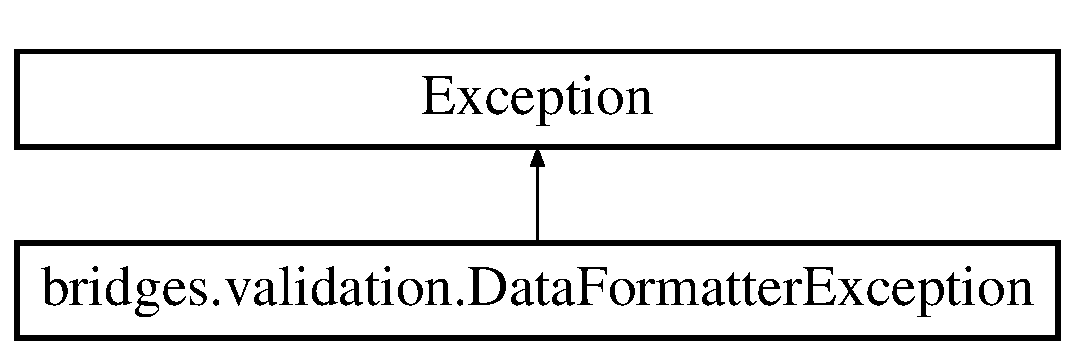
\includegraphics[height=2.000000cm]{classbridges_1_1validation_1_1_data_formatter_exception}
\end{center}
\end{figure}
\subsection*{Public Member Functions}
\begin{DoxyCompactItemize}
\item 
\hyperlink{classbridges_1_1validation_1_1_data_formatter_exception_aa922b9fa359b89c0b25eaa1efd0cfd07}{Data\+Formatter\+Exception} ()
\item 
\hyperlink{classbridges_1_1validation_1_1_data_formatter_exception_abadd66eb3ea98c1af1ff397912ed73bf}{Data\+Formatter\+Exception} (String message)
\item 
\hyperlink{classbridges_1_1validation_1_1_data_formatter_exception_ae7ce6479c3caf8077d5e34b79fe980dd}{Data\+Formatter\+Exception} (Throwable cause)
\item 
\hyperlink{classbridges_1_1validation_1_1_data_formatter_exception_acaec0fe0a826d08481207a3bac21c913}{Data\+Formatter\+Exception} (String message, Throwable cause)
\item 
String \hyperlink{classbridges_1_1validation_1_1_data_formatter_exception_ad60457ab04769d2c80e6ba77a6307ce1}{get\+Error} ()
\item 
Throwable \hyperlink{classbridges_1_1validation_1_1_data_formatter_exception_a6223e92ea95f3050d532997cb115cf2a}{get\+Cause} ()
\end{DoxyCompactItemize}
\subsection*{Public Attributes}
\begin{DoxyCompactItemize}
\item 
String \hyperlink{classbridges_1_1validation_1_1_data_formatter_exception_a8cab4688a8a80a0575bcda28e6ac7b8c}{a\+Message}
\item 
Throwable \hyperlink{classbridges_1_1validation_1_1_data_formatter_exception_ad2fdeb878690d9fc23f1316f55696ffd}{a\+Cause}
\end{DoxyCompactItemize}


\subsection{Detailed Description}
This is an extension of the Exception class adding my customized exceptions \begin{DoxyAuthor}{Author}
mihai 
\end{DoxyAuthor}


\subsection{Constructor \& Destructor Documentation}
\hypertarget{classbridges_1_1validation_1_1_data_formatter_exception_aa922b9fa359b89c0b25eaa1efd0cfd07}{}\label{classbridges_1_1validation_1_1_data_formatter_exception_aa922b9fa359b89c0b25eaa1efd0cfd07} 
\index{bridges\+::validation\+::\+Data\+Formatter\+Exception@{bridges\+::validation\+::\+Data\+Formatter\+Exception}!Data\+Formatter\+Exception@{Data\+Formatter\+Exception}}
\index{Data\+Formatter\+Exception@{Data\+Formatter\+Exception}!bridges\+::validation\+::\+Data\+Formatter\+Exception@{bridges\+::validation\+::\+Data\+Formatter\+Exception}}
\subsubsection{\texorpdfstring{Data\+Formatter\+Exception()}{DataFormatterException()}\hspace{0.1cm}{\footnotesize\ttfamily [1/4]}}
{\footnotesize\ttfamily bridges.\+validation.\+Data\+Formatter\+Exception.\+Data\+Formatter\+Exception (\begin{DoxyParamCaption}{ }\end{DoxyParamCaption})}

\hypertarget{classbridges_1_1validation_1_1_data_formatter_exception_abadd66eb3ea98c1af1ff397912ed73bf}{}\label{classbridges_1_1validation_1_1_data_formatter_exception_abadd66eb3ea98c1af1ff397912ed73bf} 
\index{bridges\+::validation\+::\+Data\+Formatter\+Exception@{bridges\+::validation\+::\+Data\+Formatter\+Exception}!Data\+Formatter\+Exception@{Data\+Formatter\+Exception}}
\index{Data\+Formatter\+Exception@{Data\+Formatter\+Exception}!bridges\+::validation\+::\+Data\+Formatter\+Exception@{bridges\+::validation\+::\+Data\+Formatter\+Exception}}
\subsubsection{\texorpdfstring{Data\+Formatter\+Exception()}{DataFormatterException()}\hspace{0.1cm}{\footnotesize\ttfamily [2/4]}}
{\footnotesize\ttfamily bridges.\+validation.\+Data\+Formatter\+Exception.\+Data\+Formatter\+Exception (\begin{DoxyParamCaption}\item[{String}]{message }\end{DoxyParamCaption})}

\hypertarget{classbridges_1_1validation_1_1_data_formatter_exception_ae7ce6479c3caf8077d5e34b79fe980dd}{}\label{classbridges_1_1validation_1_1_data_formatter_exception_ae7ce6479c3caf8077d5e34b79fe980dd} 
\index{bridges\+::validation\+::\+Data\+Formatter\+Exception@{bridges\+::validation\+::\+Data\+Formatter\+Exception}!Data\+Formatter\+Exception@{Data\+Formatter\+Exception}}
\index{Data\+Formatter\+Exception@{Data\+Formatter\+Exception}!bridges\+::validation\+::\+Data\+Formatter\+Exception@{bridges\+::validation\+::\+Data\+Formatter\+Exception}}
\subsubsection{\texorpdfstring{Data\+Formatter\+Exception()}{DataFormatterException()}\hspace{0.1cm}{\footnotesize\ttfamily [3/4]}}
{\footnotesize\ttfamily bridges.\+validation.\+Data\+Formatter\+Exception.\+Data\+Formatter\+Exception (\begin{DoxyParamCaption}\item[{Throwable}]{cause }\end{DoxyParamCaption})}

\hypertarget{classbridges_1_1validation_1_1_data_formatter_exception_acaec0fe0a826d08481207a3bac21c913}{}\label{classbridges_1_1validation_1_1_data_formatter_exception_acaec0fe0a826d08481207a3bac21c913} 
\index{bridges\+::validation\+::\+Data\+Formatter\+Exception@{bridges\+::validation\+::\+Data\+Formatter\+Exception}!Data\+Formatter\+Exception@{Data\+Formatter\+Exception}}
\index{Data\+Formatter\+Exception@{Data\+Formatter\+Exception}!bridges\+::validation\+::\+Data\+Formatter\+Exception@{bridges\+::validation\+::\+Data\+Formatter\+Exception}}
\subsubsection{\texorpdfstring{Data\+Formatter\+Exception()}{DataFormatterException()}\hspace{0.1cm}{\footnotesize\ttfamily [4/4]}}
{\footnotesize\ttfamily bridges.\+validation.\+Data\+Formatter\+Exception.\+Data\+Formatter\+Exception (\begin{DoxyParamCaption}\item[{String}]{message,  }\item[{Throwable}]{cause }\end{DoxyParamCaption})}



\subsection{Member Function Documentation}
\hypertarget{classbridges_1_1validation_1_1_data_formatter_exception_a6223e92ea95f3050d532997cb115cf2a}{}\label{classbridges_1_1validation_1_1_data_formatter_exception_a6223e92ea95f3050d532997cb115cf2a} 
\index{bridges\+::validation\+::\+Data\+Formatter\+Exception@{bridges\+::validation\+::\+Data\+Formatter\+Exception}!get\+Cause@{get\+Cause}}
\index{get\+Cause@{get\+Cause}!bridges\+::validation\+::\+Data\+Formatter\+Exception@{bridges\+::validation\+::\+Data\+Formatter\+Exception}}
\subsubsection{\texorpdfstring{get\+Cause()}{getCause()}}
{\footnotesize\ttfamily Throwable bridges.\+validation.\+Data\+Formatter\+Exception.\+get\+Cause (\begin{DoxyParamCaption}{ }\end{DoxyParamCaption})}

\hypertarget{classbridges_1_1validation_1_1_data_formatter_exception_ad60457ab04769d2c80e6ba77a6307ce1}{}\label{classbridges_1_1validation_1_1_data_formatter_exception_ad60457ab04769d2c80e6ba77a6307ce1} 
\index{bridges\+::validation\+::\+Data\+Formatter\+Exception@{bridges\+::validation\+::\+Data\+Formatter\+Exception}!get\+Error@{get\+Error}}
\index{get\+Error@{get\+Error}!bridges\+::validation\+::\+Data\+Formatter\+Exception@{bridges\+::validation\+::\+Data\+Formatter\+Exception}}
\subsubsection{\texorpdfstring{get\+Error()}{getError()}}
{\footnotesize\ttfamily String bridges.\+validation.\+Data\+Formatter\+Exception.\+get\+Error (\begin{DoxyParamCaption}{ }\end{DoxyParamCaption})}



\subsection{Member Data Documentation}
\hypertarget{classbridges_1_1validation_1_1_data_formatter_exception_ad2fdeb878690d9fc23f1316f55696ffd}{}\label{classbridges_1_1validation_1_1_data_formatter_exception_ad2fdeb878690d9fc23f1316f55696ffd} 
\index{bridges\+::validation\+::\+Data\+Formatter\+Exception@{bridges\+::validation\+::\+Data\+Formatter\+Exception}!a\+Cause@{a\+Cause}}
\index{a\+Cause@{a\+Cause}!bridges\+::validation\+::\+Data\+Formatter\+Exception@{bridges\+::validation\+::\+Data\+Formatter\+Exception}}
\subsubsection{\texorpdfstring{a\+Cause}{aCause}}
{\footnotesize\ttfamily Throwable bridges.\+validation.\+Data\+Formatter\+Exception.\+a\+Cause}

\hypertarget{classbridges_1_1validation_1_1_data_formatter_exception_a8cab4688a8a80a0575bcda28e6ac7b8c}{}\label{classbridges_1_1validation_1_1_data_formatter_exception_a8cab4688a8a80a0575bcda28e6ac7b8c} 
\index{bridges\+::validation\+::\+Data\+Formatter\+Exception@{bridges\+::validation\+::\+Data\+Formatter\+Exception}!a\+Message@{a\+Message}}
\index{a\+Message@{a\+Message}!bridges\+::validation\+::\+Data\+Formatter\+Exception@{bridges\+::validation\+::\+Data\+Formatter\+Exception}}
\subsubsection{\texorpdfstring{a\+Message}{aMessage}}
{\footnotesize\ttfamily String bridges.\+validation.\+Data\+Formatter\+Exception.\+a\+Message}



The documentation for this class was generated from the following file\+:\begin{DoxyCompactItemize}
\item 
/\+Users/kalpathi/gr/bridges/client/java/bridges16/src/main/java/edu/uncc/cs/bridges\+\_\+v21/validation/\hyperlink{_data_formatter_exception_8java}{Data\+Formatter\+Exception.\+java}\end{DoxyCompactItemize}

\hypertarget{classbridges_1_1connect_1_1_data_source}{}\section{bridges.\+connect.\+Data\+Source Class Reference}
\label{classbridges_1_1connect_1_1_data_source}\index{bridges.\+connect.\+Data\+Source@{bridges.\+connect.\+Data\+Source}}


\subsection{Detailed Description}
This class is the main B\+R\+I\+D\+G\+ES class that facilitates access to external datasets. 

The \hyperlink{classbridges_1_1connect_1_1_data_source}{Data\+Source} class provides the B\+R\+I\+D\+G\+ES A\+PI to all external datasets that are implemented in B\+R\+I\+D\+G\+ES. These include earthquake data, song data, I\+M\+DB actor/movies, Wikidata, Guttenberg book collections, Open\+Street maps, Shakespeare, play, sonnets, poems, Cancer incidence data and I\+GN games Each dataset is accessed through a function call, which typically returns a list of objects with all associated attributes. These can then be used as part of a data structure, algorithm. Some initial support to import previously built data structures is also provided. \subsection*{Public Member Functions}
\begin{DoxyCompactItemize}
\item 
List$<$ \hyperlink{classbridges_1_1data__src__dependent_1_1_earthquake_u_s_g_s}{Earthquake\+U\+S\+GS} $>$ \hyperlink{classbridges_1_1connect_1_1_data_source_af49a5212ae2bb6eed4501152276b79ad}{get\+Earthquake\+U\+S\+G\+S\+Data} (int max\+Elem)  throws I\+O\+Exception 
\item 
List$<$ \hyperlink{classbridges_1_1data__src__dependent_1_1_shakespeare}{Shakespeare} $>$ \hyperlink{classbridges_1_1connect_1_1_data_source_af2b6e5df074d0a689e8a992b1bea6f3e}{get\+Shakespeare\+Data} ()  throws Exception 
\begin{DoxyCompactList}\small\item\em This function provides access to a collection of Shakespeare plays, poems and plays. \end{DoxyCompactList}\item 
List$<$ \hyperlink{classbridges_1_1data__src__dependent_1_1_shakespeare}{Shakespeare} $>$ \hyperlink{classbridges_1_1connect_1_1_data_source_a04aa757c45139e52525d4b09156abfe1}{get\+Shakespeare\+Data} (String works)  throws Exception 
\begin{DoxyCompactList}\small\item\em This function provides access to a collection of Shakespeare plays, poems and plays. \end{DoxyCompactList}\item 
List$<$ \hyperlink{classbridges_1_1data__src__dependent_1_1_cancer_incidence}{Cancer\+Incidence} $>$ \hyperlink{classbridges_1_1connect_1_1_data_source_a7617a81fe00361c3ae6fed5873739aa2}{get\+Cancer\+Incidence\+Data} ()  throws Exception 
\item 
List$<$ \hyperlink{classbridges_1_1data__src__dependent_1_1_actor_movie_i_m_d_b}{Actor\+Movie\+I\+M\+DB} $>$ \hyperlink{classbridges_1_1connect_1_1_data_source_ab18803b850f3c867306723d1a1be337e}{get\+Actor\+Movie\+I\+M\+D\+B\+Data} (int max\+Elem)  throws I\+O\+Exception, Illegal\+Argument\+Exception 
\item 
List$<$ \hyperlink{classbridges_1_1data__src__dependent_1_1_actor_movie_i_m_d_b}{Actor\+Movie\+I\+M\+DB} $>$ \hyperlink{classbridges_1_1connect_1_1_data_source_ae44e4ed7879e2755f8c66a335d8b6ad5}{get\+Actor\+Movie\+I\+M\+D\+B\+Data2} ()  throws I\+O\+Exception 
\item 
List$<$ \hyperlink{classbridges_1_1data__src__dependent_1_1_gutenberg_book}{Gutenberg\+Book} $>$ \hyperlink{classbridges_1_1connect_1_1_data_source_aff3adc9d08624062469315f2fe059044}{get\+Gutenberg\+Book\+Meta\+Data} ()  throws I\+O\+Exception 
\item 
List$<$ \hyperlink{classbridges_1_1data__src__dependent_1_1_game}{Game} $>$ \hyperlink{classbridges_1_1connect_1_1_data_source_ab3744c6b103281724bdd832da0924312}{get\+Game\+Data} ()  throws I\+O\+Exception 
\item 
Array\+List$<$ \hyperlink{classbridges_1_1data__src__dependent_1_1_song}{Song} $>$ \hyperlink{classbridges_1_1connect_1_1_data_source_aeccb689aeacc094b0621ab5564849fa6}{get\+Song\+Data} ()  throws I\+O\+Exception 
\item 
\hyperlink{classbridges_1_1data__src__dependent_1_1_song}{Song} \hyperlink{classbridges_1_1connect_1_1_data_source_a935ea2005b7de3cb22c1e55027b81460}{get\+Song} (String song\+Title, String artist\+Name)  throws I\+O\+Exception 
\item 
\hyperlink{classbridges_1_1data__src__dependent_1_1_amenity_data}{Amenity\+Data} \hyperlink{classbridges_1_1connect_1_1_data_source_aa25f4d7521aa1ad788b60816eb2088db}{get\+Amenity\+Data} (String location, String amenity)  throws I\+O\+Exception 
\item 
\hyperlink{classbridges_1_1data__src__dependent_1_1_amenity_data}{Amenity\+Data} \hyperlink{classbridges_1_1connect_1_1_data_source_a4fdb7ddbeecaa30a4e6972c0b537bb44}{get\+Amenity\+Data} (double min\+Lat, double min\+Lon, double max\+Lat, double max\+Lon, String amenity)  throws I\+O\+Exception 
\item 
\hyperlink{classbridges_1_1data__src__dependent_1_1_elevation_data}{Elevation\+Data} \hyperlink{classbridges_1_1connect_1_1_data_source_ac3aec28786d148e6b3554c78679bb4c2}{get\+Elevation\+Data} (double min\+Lat, double min\+Lon, double max\+Lat, double max\+Lon, double res)  throws I\+O\+Exception 
\item 
String \hyperlink{classbridges_1_1connect_1_1_data_source_af2f6cd7172acb64b2ba49f134b5391f8}{get\+Assignment\+J\+S\+ON} (String user, int assignment, int subassignment)  throws I\+O\+Exception 
\item 
String \hyperlink{classbridges_1_1connect_1_1_data_source_af55c85da71b588f64ff4b46dbacab7f4}{get\+Assignment\+J\+S\+ON} (String user, int assignment)  throws I\+O\+Exception 
\item 
\hyperlink{classbridges_1_1base_1_1_color_grid}{Color\+Grid} \hyperlink{classbridges_1_1connect_1_1_data_source_a7bddb93c9196a1109f2bf36054500ed8}{get\+Color\+Grid\+From\+Assignment} (String user, int assignment, int subassignment)  throws I\+O\+Exception 
\item 
\hyperlink{classbridges_1_1base_1_1_color_grid}{Color\+Grid} \hyperlink{classbridges_1_1connect_1_1_data_source_a19356653cc7ae56f57f5d28994048ee3}{get\+Color\+Grid\+From\+Assignment} (String user, int assignment)  throws I\+O\+Exception 
\end{DoxyCompactItemize}
\subsection*{Static Public Member Functions}
\begin{DoxyCompactItemize}
\item 
static \hyperlink{classbridges_1_1data__src__dependent_1_1_osm_data}{Osm\+Data} \hyperlink{classbridges_1_1connect_1_1_data_source_a836aff0a3c4003cbc21d65d949d5f985}{get\+Osm\+Data} (String location)  throws I\+O\+Exception 
\item 
static \hyperlink{classbridges_1_1data__src__dependent_1_1_osm_data}{Osm\+Data} \hyperlink{classbridges_1_1connect_1_1_data_source_a92e5a1b0104cce618012c4ec9c84e8aa}{get\+Osm\+Data} (String location, String level)  throws I\+O\+Exception 
\item 
static \hyperlink{classbridges_1_1data__src__dependent_1_1_osm_data}{Osm\+Data} \hyperlink{classbridges_1_1connect_1_1_data_source_ae14038856a8b48b0b75ddd43f58059ad}{get\+Osm\+Data} (double min\+Lat, double min\+Lon, double max\+Lat, double max\+Lon)  throws I\+O\+Exception 
\item 
static \hyperlink{classbridges_1_1data__src__dependent_1_1_osm_data}{Osm\+Data} \hyperlink{classbridges_1_1connect_1_1_data_source_a30e8c815c2d2bab1ef62fa5bea27b42d}{get\+Osm\+Data} (double min\+Lat, double min\+Lon, double max\+Lat, double max\+Lon, String level)  throws I\+O\+Exception 
\item 
static Array\+List$<$ \hyperlink{classbridges_1_1data__src__dependent_1_1_actor_movie_wikidata}{Actor\+Movie\+Wikidata} $>$ \hyperlink{classbridges_1_1connect_1_1_data_source_ad06946cc793bb990eeb3b9418ade1479}{get\+Wikidata\+Actor\+Movie} (int year\+Begin, int year\+End)  throws I\+O\+Exception 
\begin{DoxyCompactList}\small\item\em This function returns the Movie and Actors playing in them between two years from Wiki\+Data. \end{DoxyCompactList}\item 
static \hyperlink{classbridges_1_1base_1_1_color_grid}{Color\+Grid} \hyperlink{classbridges_1_1connect_1_1_data_source_a46104188d82c85573d1da98a5f379bd5}{get\+Color\+Grid\+From\+Assignment} (String server, String user, int assignment, int subassignment)  throws I\+O\+Exception 
\begin{DoxyCompactList}\small\item\em Reconstruct a Color\+Grid from an existing Color\+Grid on the \hyperlink{classbridges_1_1connect_1_1_bridges}{Bridges} server. \end{DoxyCompactList}\item 
static \hyperlink{classbridges_1_1base_1_1_color_grid}{bridges.\+base.\+Color\+Grid} \hyperlink{classbridges_1_1connect_1_1_data_source_acd2dd966d1ef624c9e31c1dab69aaf9b}{get\+Color\+Grid\+From\+Assignment} (String server, String user, int assignment)  throws I\+O\+Exception 
\begin{DoxyCompactList}\small\item\em Reconstruct a Color\+Grid from an existing Color\+Grid on the \hyperlink{classbridges_1_1connect_1_1_bridges}{Bridges} server. \end{DoxyCompactList}\item 
static String \hyperlink{classbridges_1_1connect_1_1_data_source_ab95eceb71fd0ff1cdc5558a53d47d5c4}{get\+Assignment} (String server, String user, int assignment, int subassignment)  throws I\+O\+Exception 
\item 
static String \hyperlink{classbridges_1_1connect_1_1_data_source_ac3487262c29278bf2e16da45adf3bc89}{get\+Assignment} (String server, String user, int assignment)  throws I\+O\+Exception, Exception 
\end{DoxyCompactItemize}


\subsection{Member Function Documentation}
\mbox{\Hypertarget{classbridges_1_1connect_1_1_data_source_ab18803b850f3c867306723d1a1be337e}\label{classbridges_1_1connect_1_1_data_source_ab18803b850f3c867306723d1a1be337e}} 
\index{bridges\+::connect\+::\+Data\+Source@{bridges\+::connect\+::\+Data\+Source}!get\+Actor\+Movie\+I\+M\+D\+B\+Data@{get\+Actor\+Movie\+I\+M\+D\+B\+Data}}
\index{get\+Actor\+Movie\+I\+M\+D\+B\+Data@{get\+Actor\+Movie\+I\+M\+D\+B\+Data}!bridges\+::connect\+::\+Data\+Source@{bridges\+::connect\+::\+Data\+Source}}
\subsubsection{\texorpdfstring{get\+Actor\+Movie\+I\+M\+D\+B\+Data()}{getActorMovieIMDBData()}}
{\footnotesize\ttfamily List$<$\hyperlink{classbridges_1_1data__src__dependent_1_1_actor_movie_i_m_d_b}{Actor\+Movie\+I\+M\+DB}$>$ bridges.\+connect.\+Data\+Source.\+get\+Actor\+Movie\+I\+M\+D\+B\+Data (\begin{DoxyParamCaption}\item[{int}]{max\+Elem }\end{DoxyParamCaption}) throws I\+O\+Exception, Illegal\+Argument\+Exception}

Get Actor\+Movie I\+M\+DB Data retrieved, formatted into a list of Actor\+Movie\+I\+M\+DB objects


\begin{DoxyParams}{Parameters}
{\em max\+Elem} & the number of actor/movie pairs \\
\hline
\end{DoxyParams}

\begin{DoxyExceptions}{Exceptions}
{\em Exception} & if the request fails\\
\hline
\end{DoxyExceptions}
\begin{DoxyReturn}{Returns}
a list of Actor\+Movie\+I\+M\+DB objects, but only actor and movie fields in this version 
\end{DoxyReturn}
\mbox{\Hypertarget{classbridges_1_1connect_1_1_data_source_ae44e4ed7879e2755f8c66a335d8b6ad5}\label{classbridges_1_1connect_1_1_data_source_ae44e4ed7879e2755f8c66a335d8b6ad5}} 
\index{bridges\+::connect\+::\+Data\+Source@{bridges\+::connect\+::\+Data\+Source}!get\+Actor\+Movie\+I\+M\+D\+B\+Data2@{get\+Actor\+Movie\+I\+M\+D\+B\+Data2}}
\index{get\+Actor\+Movie\+I\+M\+D\+B\+Data2@{get\+Actor\+Movie\+I\+M\+D\+B\+Data2}!bridges\+::connect\+::\+Data\+Source@{bridges\+::connect\+::\+Data\+Source}}
\subsubsection{\texorpdfstring{get\+Actor\+Movie\+I\+M\+D\+B\+Data2()}{getActorMovieIMDBData2()}}
{\footnotesize\ttfamily List$<$\hyperlink{classbridges_1_1data__src__dependent_1_1_actor_movie_i_m_d_b}{Actor\+Movie\+I\+M\+DB}$>$ bridges.\+connect.\+Data\+Source.\+get\+Actor\+Movie\+I\+M\+D\+B\+Data2 (\begin{DoxyParamCaption}{ }\end{DoxyParamCaption}) throws I\+O\+Exception}

This helper function provides access to a second curated I\+M\+DB dataset; the data is retrieved, formatted into a list of Actor\+Movie\+I\+M\+DB objects

This version of the I\+M\+DB Actor/\+Movie data contains for each record, actor name, movie name, movie genres, movie rating; refer to 

~~~~~\href{http://bridgesuncc.github.io/datasets.html}{\tt http\+://bridgesuncc.\+github.\+io/datasets.\+html} 

for more information and to look at the dataset.


\begin{DoxyExceptions}{Exceptions}
{\em Exception} & if the request fails\\
\hline
\end{DoxyExceptions}
\begin{DoxyReturn}{Returns}
a list of Actor\+Movie\+I\+M\+DB objects 
\end{DoxyReturn}
\mbox{\Hypertarget{classbridges_1_1connect_1_1_data_source_aa25f4d7521aa1ad788b60816eb2088db}\label{classbridges_1_1connect_1_1_data_source_aa25f4d7521aa1ad788b60816eb2088db}} 
\index{bridges\+::connect\+::\+Data\+Source@{bridges\+::connect\+::\+Data\+Source}!get\+Amenity\+Data@{get\+Amenity\+Data}}
\index{get\+Amenity\+Data@{get\+Amenity\+Data}!bridges\+::connect\+::\+Data\+Source@{bridges\+::connect\+::\+Data\+Source}}
\subsubsection{\texorpdfstring{get\+Amenity\+Data()}{getAmenityData()}\hspace{0.1cm}{\footnotesize\ttfamily [1/2]}}
{\footnotesize\ttfamily \hyperlink{classbridges_1_1data__src__dependent_1_1_amenity_data}{Amenity\+Data} bridges.\+connect.\+Data\+Source.\+get\+Amenity\+Data (\begin{DoxyParamCaption}\item[{String}]{location,  }\item[{String}]{amenity }\end{DoxyParamCaption}) throws I\+O\+Exception}

This method retrieves the specified amenity related data given a location from a specified openstreet mmap location


\begin{DoxyParams}{Parameters}
{\em location} & city/town from where amenity data is sought \\
\hline
{\em amenity} & amenity type \\
\hline
\end{DoxyParams}

\begin{DoxyExceptions}{Exceptions}
{\em exception} & \\
\hline
\end{DoxyExceptions}
\mbox{\Hypertarget{classbridges_1_1connect_1_1_data_source_a4fdb7ddbeecaa30a4e6972c0b537bb44}\label{classbridges_1_1connect_1_1_data_source_a4fdb7ddbeecaa30a4e6972c0b537bb44}} 
\index{bridges\+::connect\+::\+Data\+Source@{bridges\+::connect\+::\+Data\+Source}!get\+Amenity\+Data@{get\+Amenity\+Data}}
\index{get\+Amenity\+Data@{get\+Amenity\+Data}!bridges\+::connect\+::\+Data\+Source@{bridges\+::connect\+::\+Data\+Source}}
\subsubsection{\texorpdfstring{get\+Amenity\+Data()}{getAmenityData()}\hspace{0.1cm}{\footnotesize\ttfamily [2/2]}}
{\footnotesize\ttfamily \hyperlink{classbridges_1_1data__src__dependent_1_1_amenity_data}{Amenity\+Data} bridges.\+connect.\+Data\+Source.\+get\+Amenity\+Data (\begin{DoxyParamCaption}\item[{double}]{min\+Lat,  }\item[{double}]{min\+Lon,  }\item[{double}]{max\+Lat,  }\item[{double}]{max\+Lon,  }\item[{String}]{amenity }\end{DoxyParamCaption}) throws I\+O\+Exception}

This method retrieves the specified amenity related data given a bounding box of a region, from a Open Street map


\begin{DoxyParams}{Parameters}
{\em min\+Lat} & minimum latitude \\
\hline
{\em min\+Lon} & minimumm longitude \\
\hline
{\em max\+Lat} & maximum latitude \\
\hline
{\em max\+Lon} & maximum longitude \\
\hline
{\em amenity} & amenity type \\
\hline
\end{DoxyParams}

\begin{DoxyExceptions}{Exceptions}
{\em exception} & \\
\hline
\end{DoxyExceptions}
\mbox{\Hypertarget{classbridges_1_1connect_1_1_data_source_ab95eceb71fd0ff1cdc5558a53d47d5c4}\label{classbridges_1_1connect_1_1_data_source_ab95eceb71fd0ff1cdc5558a53d47d5c4}} 
\index{bridges\+::connect\+::\+Data\+Source@{bridges\+::connect\+::\+Data\+Source}!get\+Assignment@{get\+Assignment}}
\index{get\+Assignment@{get\+Assignment}!bridges\+::connect\+::\+Data\+Source@{bridges\+::connect\+::\+Data\+Source}}
\subsubsection{\texorpdfstring{get\+Assignment()}{getAssignment()}\hspace{0.1cm}{\footnotesize\ttfamily [1/2]}}
{\footnotesize\ttfamily static String bridges.\+connect.\+Data\+Source.\+get\+Assignment (\begin{DoxyParamCaption}\item[{String}]{server,  }\item[{String}]{user,  }\item[{int}]{assignment,  }\item[{int}]{subassignment }\end{DoxyParamCaption}) throws I\+O\+Exception\hspace{0.3cm}{\ttfamily [static]}}

\mbox{\Hypertarget{classbridges_1_1connect_1_1_data_source_ac3487262c29278bf2e16da45adf3bc89}\label{classbridges_1_1connect_1_1_data_source_ac3487262c29278bf2e16da45adf3bc89}} 
\index{bridges\+::connect\+::\+Data\+Source@{bridges\+::connect\+::\+Data\+Source}!get\+Assignment@{get\+Assignment}}
\index{get\+Assignment@{get\+Assignment}!bridges\+::connect\+::\+Data\+Source@{bridges\+::connect\+::\+Data\+Source}}
\subsubsection{\texorpdfstring{get\+Assignment()}{getAssignment()}\hspace{0.1cm}{\footnotesize\ttfamily [2/2]}}
{\footnotesize\ttfamily static String bridges.\+connect.\+Data\+Source.\+get\+Assignment (\begin{DoxyParamCaption}\item[{String}]{server,  }\item[{String}]{user,  }\item[{int}]{assignment }\end{DoxyParamCaption}) throws I\+O\+Exception, Exception\hspace{0.3cm}{\ttfamily [static]}}

\mbox{\Hypertarget{classbridges_1_1connect_1_1_data_source_af2f6cd7172acb64b2ba49f134b5391f8}\label{classbridges_1_1connect_1_1_data_source_af2f6cd7172acb64b2ba49f134b5391f8}} 
\index{bridges\+::connect\+::\+Data\+Source@{bridges\+::connect\+::\+Data\+Source}!get\+Assignment\+J\+S\+ON@{get\+Assignment\+J\+S\+ON}}
\index{get\+Assignment\+J\+S\+ON@{get\+Assignment\+J\+S\+ON}!bridges\+::connect\+::\+Data\+Source@{bridges\+::connect\+::\+Data\+Source}}
\subsubsection{\texorpdfstring{get\+Assignment\+J\+S\+O\+N()}{getAssignmentJSON()}\hspace{0.1cm}{\footnotesize\ttfamily [1/2]}}
{\footnotesize\ttfamily String bridges.\+connect.\+Data\+Source.\+get\+Assignment\+J\+S\+ON (\begin{DoxyParamCaption}\item[{String}]{user,  }\item[{int}]{assignment,  }\item[{int}]{subassignment }\end{DoxyParamCaption}) throws I\+O\+Exception}

This function obtains the J\+S\+ON representation of a particular subassignment.

\begin{DoxyReturn}{Returns}
a string that is the J\+S\+ON representation of the subassignment as stored by the \hyperlink{classbridges_1_1connect_1_1_bridges}{Bridges} server. 
\end{DoxyReturn}

\begin{DoxyParams}{Parameters}
{\em user} & the name of the user who uploaded the assignment \\
\hline
{\em assignment} & the ID of the assignment to get \\
\hline
{\em subassignment} & the ID of the subassignment to get \\
\hline
\end{DoxyParams}
\mbox{\Hypertarget{classbridges_1_1connect_1_1_data_source_af55c85da71b588f64ff4b46dbacab7f4}\label{classbridges_1_1connect_1_1_data_source_af55c85da71b588f64ff4b46dbacab7f4}} 
\index{bridges\+::connect\+::\+Data\+Source@{bridges\+::connect\+::\+Data\+Source}!get\+Assignment\+J\+S\+ON@{get\+Assignment\+J\+S\+ON}}
\index{get\+Assignment\+J\+S\+ON@{get\+Assignment\+J\+S\+ON}!bridges\+::connect\+::\+Data\+Source@{bridges\+::connect\+::\+Data\+Source}}
\subsubsection{\texorpdfstring{get\+Assignment\+J\+S\+O\+N()}{getAssignmentJSON()}\hspace{0.1cm}{\footnotesize\ttfamily [2/2]}}
{\footnotesize\ttfamily String bridges.\+connect.\+Data\+Source.\+get\+Assignment\+J\+S\+ON (\begin{DoxyParamCaption}\item[{String}]{user,  }\item[{int}]{assignment }\end{DoxyParamCaption}) throws I\+O\+Exception}

This function obtains the J\+S\+ON representation of a particular subassignment.

\begin{DoxyReturn}{Returns}
a string that is the J\+S\+ON representation of the subassignment as stored by the \hyperlink{classbridges_1_1connect_1_1_bridges}{Bridges} server. 
\end{DoxyReturn}

\begin{DoxyParams}{Parameters}
{\em user} & the name of the user who uploaded the assignment \\
\hline
{\em assignment} & the ID of the assignment to get \\
\hline
\end{DoxyParams}
\mbox{\Hypertarget{classbridges_1_1connect_1_1_data_source_a7617a81fe00361c3ae6fed5873739aa2}\label{classbridges_1_1connect_1_1_data_source_a7617a81fe00361c3ae6fed5873739aa2}} 
\index{bridges\+::connect\+::\+Data\+Source@{bridges\+::connect\+::\+Data\+Source}!get\+Cancer\+Incidence\+Data@{get\+Cancer\+Incidence\+Data}}
\index{get\+Cancer\+Incidence\+Data@{get\+Cancer\+Incidence\+Data}!bridges\+::connect\+::\+Data\+Source@{bridges\+::connect\+::\+Data\+Source}}
\subsubsection{\texorpdfstring{get\+Cancer\+Incidence\+Data()}{getCancerIncidenceData()}}
{\footnotesize\ttfamily List$<$\hyperlink{classbridges_1_1data__src__dependent_1_1_cancer_incidence}{Cancer\+Incidence}$>$ bridges.\+connect.\+Data\+Source.\+get\+Cancer\+Incidence\+Data (\begin{DoxyParamCaption}{ }\end{DoxyParamCaption}) throws Exception}

This helper function provides access to a cancer dataset from C\+DC \href{https://www.cdc.gov/cancer/npcr/uscs/download_data.htm}{\tt https\+://www.\+cdc.\+gov/cancer/npcr/uscs/download\+\_\+data.\+htm} and curated by Austin (Cory) Bart as part of the Corgis data collection \href{https://think.cs.vt.edu/corgis/}{\tt https\+://think.\+cs.\+vt.\+edu/corgis/}

Each record in this collection has a number of fields detailed in the Cancer\+Incidence class.

For more information and to look at the data, refer to 

~~~~~\href{http://bridgesuncc.github.io/datasets.html}{\tt http\+://bridgesuncc.\+github.\+io/datasets.\+html} 


\begin{DoxyExceptions}{Exceptions}
{\em Exception} & if the request fails\\
\hline
\end{DoxyExceptions}
\begin{DoxyReturn}{Returns}
a list of Cancer incidence objects. 
\end{DoxyReturn}
\mbox{\Hypertarget{classbridges_1_1connect_1_1_data_source_a7bddb93c9196a1109f2bf36054500ed8}\label{classbridges_1_1connect_1_1_data_source_a7bddb93c9196a1109f2bf36054500ed8}} 
\index{bridges\+::connect\+::\+Data\+Source@{bridges\+::connect\+::\+Data\+Source}!get\+Color\+Grid\+From\+Assignment@{get\+Color\+Grid\+From\+Assignment}}
\index{get\+Color\+Grid\+From\+Assignment@{get\+Color\+Grid\+From\+Assignment}!bridges\+::connect\+::\+Data\+Source@{bridges\+::connect\+::\+Data\+Source}}
\subsubsection{\texorpdfstring{get\+Color\+Grid\+From\+Assignment()}{getColorGridFromAssignment()}\hspace{0.1cm}{\footnotesize\ttfamily [1/4]}}
{\footnotesize\ttfamily \hyperlink{classbridges_1_1base_1_1_color_grid}{Color\+Grid} bridges.\+connect.\+Data\+Source.\+get\+Color\+Grid\+From\+Assignment (\begin{DoxyParamCaption}\item[{String}]{user,  }\item[{int}]{assignment,  }\item[{int}]{subassignment }\end{DoxyParamCaption}) throws I\+O\+Exception}

Reconstruct a Color\+Grid from an existing Color\+Grid on the \hyperlink{classbridges_1_1connect_1_1_bridges}{Bridges} server

\begin{DoxyReturn}{Returns}
the Color\+Grid stored in the bridges server 
\end{DoxyReturn}

\begin{DoxyParams}{Parameters}
{\em user} & the name of the user who uploaded the assignment \\
\hline
{\em assignment} & the ID of the assignment to get \\
\hline
{\em subassignment} & the ID of the subassignment to get \\
\hline
\end{DoxyParams}
\mbox{\Hypertarget{classbridges_1_1connect_1_1_data_source_a19356653cc7ae56f57f5d28994048ee3}\label{classbridges_1_1connect_1_1_data_source_a19356653cc7ae56f57f5d28994048ee3}} 
\index{bridges\+::connect\+::\+Data\+Source@{bridges\+::connect\+::\+Data\+Source}!get\+Color\+Grid\+From\+Assignment@{get\+Color\+Grid\+From\+Assignment}}
\index{get\+Color\+Grid\+From\+Assignment@{get\+Color\+Grid\+From\+Assignment}!bridges\+::connect\+::\+Data\+Source@{bridges\+::connect\+::\+Data\+Source}}
\subsubsection{\texorpdfstring{get\+Color\+Grid\+From\+Assignment()}{getColorGridFromAssignment()}\hspace{0.1cm}{\footnotesize\ttfamily [2/4]}}
{\footnotesize\ttfamily \hyperlink{classbridges_1_1base_1_1_color_grid}{Color\+Grid} bridges.\+connect.\+Data\+Source.\+get\+Color\+Grid\+From\+Assignment (\begin{DoxyParamCaption}\item[{String}]{user,  }\item[{int}]{assignment }\end{DoxyParamCaption}) throws I\+O\+Exception}

Reconstruct a Color\+Grid from an existing Color\+Grid on the \hyperlink{classbridges_1_1connect_1_1_bridges}{Bridges} server

\begin{DoxyReturn}{Returns}
the Color\+Grid stored in the bridges server 
\end{DoxyReturn}

\begin{DoxyParams}{Parameters}
{\em user} & the name of the user who uploaded the assignment \\
\hline
{\em assignment} & the ID of the assignment to get \\
\hline
\end{DoxyParams}
\mbox{\Hypertarget{classbridges_1_1connect_1_1_data_source_a46104188d82c85573d1da98a5f379bd5}\label{classbridges_1_1connect_1_1_data_source_a46104188d82c85573d1da98a5f379bd5}} 
\index{bridges\+::connect\+::\+Data\+Source@{bridges\+::connect\+::\+Data\+Source}!get\+Color\+Grid\+From\+Assignment@{get\+Color\+Grid\+From\+Assignment}}
\index{get\+Color\+Grid\+From\+Assignment@{get\+Color\+Grid\+From\+Assignment}!bridges\+::connect\+::\+Data\+Source@{bridges\+::connect\+::\+Data\+Source}}
\subsubsection{\texorpdfstring{get\+Color\+Grid\+From\+Assignment()}{getColorGridFromAssignment()}\hspace{0.1cm}{\footnotesize\ttfamily [3/4]}}
{\footnotesize\ttfamily static \hyperlink{classbridges_1_1base_1_1_color_grid}{Color\+Grid} bridges.\+connect.\+Data\+Source.\+get\+Color\+Grid\+From\+Assignment (\begin{DoxyParamCaption}\item[{String}]{server,  }\item[{String}]{user,  }\item[{int}]{assignment,  }\item[{int}]{subassignment }\end{DoxyParamCaption}) throws I\+O\+Exception\hspace{0.3cm}{\ttfamily [static]}}



Reconstruct a Color\+Grid from an existing Color\+Grid on the \hyperlink{classbridges_1_1connect_1_1_bridges}{Bridges} server. 


\begin{DoxyParams}{Parameters}
{\em server} & base U\+RL of the \hyperlink{classbridges_1_1connect_1_1_bridges}{Bridges} service \\
\hline
{\em user} & the name of the user who uploaded the assignment \\
\hline
{\em assignment} & the ID of the assignment to get \\
\hline
{\em subassignment} & the ID of the subassignment to get \\
\hline
\end{DoxyParams}
\begin{DoxyReturn}{Returns}
the Color\+Grid stored in the bridges server 
\end{DoxyReturn}
\mbox{\Hypertarget{classbridges_1_1connect_1_1_data_source_acd2dd966d1ef624c9e31c1dab69aaf9b}\label{classbridges_1_1connect_1_1_data_source_acd2dd966d1ef624c9e31c1dab69aaf9b}} 
\index{bridges\+::connect\+::\+Data\+Source@{bridges\+::connect\+::\+Data\+Source}!get\+Color\+Grid\+From\+Assignment@{get\+Color\+Grid\+From\+Assignment}}
\index{get\+Color\+Grid\+From\+Assignment@{get\+Color\+Grid\+From\+Assignment}!bridges\+::connect\+::\+Data\+Source@{bridges\+::connect\+::\+Data\+Source}}
\subsubsection{\texorpdfstring{get\+Color\+Grid\+From\+Assignment()}{getColorGridFromAssignment()}\hspace{0.1cm}{\footnotesize\ttfamily [4/4]}}
{\footnotesize\ttfamily static \hyperlink{classbridges_1_1base_1_1_color_grid}{bridges.\+base.\+Color\+Grid} bridges.\+connect.\+Data\+Source.\+get\+Color\+Grid\+From\+Assignment (\begin{DoxyParamCaption}\item[{String}]{server,  }\item[{String}]{user,  }\item[{int}]{assignment }\end{DoxyParamCaption}) throws I\+O\+Exception\hspace{0.3cm}{\ttfamily [static]}}



Reconstruct a Color\+Grid from an existing Color\+Grid on the \hyperlink{classbridges_1_1connect_1_1_bridges}{Bridges} server. 


\begin{DoxyParams}{Parameters}
{\em server} & base U\+RL of the \hyperlink{classbridges_1_1connect_1_1_bridges}{Bridges} service \\
\hline
{\em user} & the name of the user who uploaded the assignment \\
\hline
{\em assignment} & the ID of the assignment to get \\
\hline
\end{DoxyParams}
\begin{DoxyReturn}{Returns}
the Color\+Grid stored in the bridges server 
\end{DoxyReturn}
\mbox{\Hypertarget{classbridges_1_1connect_1_1_data_source_af49a5212ae2bb6eed4501152276b79ad}\label{classbridges_1_1connect_1_1_data_source_af49a5212ae2bb6eed4501152276b79ad}} 
\index{bridges\+::connect\+::\+Data\+Source@{bridges\+::connect\+::\+Data\+Source}!get\+Earthquake\+U\+S\+G\+S\+Data@{get\+Earthquake\+U\+S\+G\+S\+Data}}
\index{get\+Earthquake\+U\+S\+G\+S\+Data@{get\+Earthquake\+U\+S\+G\+S\+Data}!bridges\+::connect\+::\+Data\+Source@{bridges\+::connect\+::\+Data\+Source}}
\subsubsection{\texorpdfstring{get\+Earthquake\+U\+S\+G\+S\+Data()}{getEarthquakeUSGSData()}}
{\footnotesize\ttfamily List$<$\hyperlink{classbridges_1_1data__src__dependent_1_1_earthquake_u_s_g_s}{Earthquake\+U\+S\+GS}$>$ bridges.\+connect.\+Data\+Source.\+get\+Earthquake\+U\+S\+G\+S\+Data (\begin{DoxyParamCaption}\item[{int}]{max\+Elem }\end{DoxyParamCaption}) throws I\+O\+Exception}

This helper function provides a simple A\+PI to retrieve current U\+S\+GS earthquake Tweet data from the U\+S\+GS website (\href{https://earthquake.usgs.gov/earthquakes/map/}{\tt https\+://earthquake.\+usgs.\+gov/earthquakes/map/}); The data is retrieved and formatted into a list of Earthquake\+U\+S\+GS objects.

More information on the dataset can be found at \href{http://bridgesuncc.github.io/datasets.html}{\tt http\+://bridgesuncc.\+github.\+io/datasets.\+html}


\begin{DoxyParams}{Parameters}
{\em max\+Elem} & the number of earthquake records retrieved, limited to 5000 \\
\hline
\end{DoxyParams}

\begin{DoxyExceptions}{Exceptions}
{\em Exception} & if the request fails\\
\hline
\end{DoxyExceptions}
\begin{DoxyReturn}{Returns}
a list of earthquake records 
\end{DoxyReturn}
\mbox{\Hypertarget{classbridges_1_1connect_1_1_data_source_ac3aec28786d148e6b3554c78679bb4c2}\label{classbridges_1_1connect_1_1_data_source_ac3aec28786d148e6b3554c78679bb4c2}} 
\index{bridges\+::connect\+::\+Data\+Source@{bridges\+::connect\+::\+Data\+Source}!get\+Elevation\+Data@{get\+Elevation\+Data}}
\index{get\+Elevation\+Data@{get\+Elevation\+Data}!bridges\+::connect\+::\+Data\+Source@{bridges\+::connect\+::\+Data\+Source}}
\subsubsection{\texorpdfstring{get\+Elevation\+Data()}{getElevationData()}}
{\footnotesize\ttfamily \hyperlink{classbridges_1_1data__src__dependent_1_1_elevation_data}{Elevation\+Data} bridges.\+connect.\+Data\+Source.\+get\+Elevation\+Data (\begin{DoxyParamCaption}\item[{double}]{min\+Lat,  }\item[{double}]{min\+Lon,  }\item[{double}]{max\+Lat,  }\item[{double}]{max\+Lon,  }\item[{double}]{res }\end{DoxyParamCaption}) throws I\+O\+Exception}

This method retrieves the elevation map of a region given the lat/long range (bounding box) and resolution level Note that the Elevation\+Data that is returned may have slightly different location and resolution.


\begin{DoxyParams}{Parameters}
{\em min\+Lat} & minimum latitude requested \\
\hline
{\em min\+Lon} & minimum longitude requested \\
\hline
{\em max\+Lat} & maximum latitude requested \\
\hline
{\em max\+Lon} & maximum longitude requested \\
\hline
{\em res} & spatial resolution, aka the distance between two samples (in degrees) \\
\hline
\end{DoxyParams}
\begin{DoxyReturn}{Returns}
a Elevation\+Data object mapping a region close to the box requested 
\end{DoxyReturn}
\mbox{\Hypertarget{classbridges_1_1connect_1_1_data_source_ab3744c6b103281724bdd832da0924312}\label{classbridges_1_1connect_1_1_data_source_ab3744c6b103281724bdd832da0924312}} 
\index{bridges\+::connect\+::\+Data\+Source@{bridges\+::connect\+::\+Data\+Source}!get\+Game\+Data@{get\+Game\+Data}}
\index{get\+Game\+Data@{get\+Game\+Data}!bridges\+::connect\+::\+Data\+Source@{bridges\+::connect\+::\+Data\+Source}}
\subsubsection{\texorpdfstring{get\+Game\+Data()}{getGameData()}}
{\footnotesize\ttfamily List$<$\hyperlink{classbridges_1_1data__src__dependent_1_1_game}{Game}$>$ bridges.\+connect.\+Data\+Source.\+get\+Game\+Data (\begin{DoxyParamCaption}{ }\end{DoxyParamCaption}) throws I\+O\+Exception}

This helper function provides access to the meta-\/data of the video game collection.

Each record in this collection has information on game title, platform, rating, and genre. For more information and to look at the data, refer to 

~~~~~\href{http://bridgesuncc.github.io/datasets.html}{\tt http\+://bridgesuncc.\+github.\+io/datasets.\+html} 


\begin{DoxyExceptions}{Exceptions}
{\em Exception} & if the request fails\\
\hline
\end{DoxyExceptions}
\begin{DoxyReturn}{Returns}
a list of Game objects. 
\end{DoxyReturn}
\mbox{\Hypertarget{classbridges_1_1connect_1_1_data_source_aff3adc9d08624062469315f2fe059044}\label{classbridges_1_1connect_1_1_data_source_aff3adc9d08624062469315f2fe059044}} 
\index{bridges\+::connect\+::\+Data\+Source@{bridges\+::connect\+::\+Data\+Source}!get\+Gutenberg\+Book\+Meta\+Data@{get\+Gutenberg\+Book\+Meta\+Data}}
\index{get\+Gutenberg\+Book\+Meta\+Data@{get\+Gutenberg\+Book\+Meta\+Data}!bridges\+::connect\+::\+Data\+Source@{bridges\+::connect\+::\+Data\+Source}}
\subsubsection{\texorpdfstring{get\+Gutenberg\+Book\+Meta\+Data()}{getGutenbergBookMetaData()}}
{\footnotesize\ttfamily List$<$\hyperlink{classbridges_1_1data__src__dependent_1_1_gutenberg_book}{Gutenberg\+Book}$>$ bridges.\+connect.\+Data\+Source.\+get\+Gutenberg\+Book\+Meta\+Data (\begin{DoxyParamCaption}{ }\end{DoxyParamCaption}) throws I\+O\+Exception}

This helper function provides access to the meta-\/data of the Gutenberg book collection (about 1000 books); the data is retrieved, formatted into a list of Gutenberg\+Book objects.

Each book in this collection has for each record, information on author (name, birth, death), title, languages, genres, subjects, metrics(number of chars, words, sentences, difficult words), url downloads. More information and commands to access the data can be found at 

~~~~~\href{http://bridgesuncc.github.io/datasets.html}{\tt http\+://bridgesuncc.\+github.\+io/datasets.\+html} ~\newline
 for more information and to look at the dataset.


\begin{DoxyExceptions}{Exceptions}
{\em Exception} & if the request fails\\
\hline
\end{DoxyExceptions}
\begin{DoxyReturn}{Returns}
a list of Gutenberg\+Book objects 
\end{DoxyReturn}
\mbox{\Hypertarget{classbridges_1_1connect_1_1_data_source_a836aff0a3c4003cbc21d65d949d5f985}\label{classbridges_1_1connect_1_1_data_source_a836aff0a3c4003cbc21d65d949d5f985}} 
\index{bridges\+::connect\+::\+Data\+Source@{bridges\+::connect\+::\+Data\+Source}!get\+Osm\+Data@{get\+Osm\+Data}}
\index{get\+Osm\+Data@{get\+Osm\+Data}!bridges\+::connect\+::\+Data\+Source@{bridges\+::connect\+::\+Data\+Source}}
\subsubsection{\texorpdfstring{get\+Osm\+Data()}{getOsmData()}\hspace{0.1cm}{\footnotesize\ttfamily [1/4]}}
{\footnotesize\ttfamily static \hyperlink{classbridges_1_1data__src__dependent_1_1_osm_data}{Osm\+Data} bridges.\+connect.\+Data\+Source.\+get\+Osm\+Data (\begin{DoxyParamCaption}\item[{String}]{location }\end{DoxyParamCaption}) throws I\+O\+Exception\hspace{0.3cm}{\ttfamily [static]}}

Generates Open Street Map U\+RL request for a given location at general level of details and returns the map data 
\begin{DoxyParams}{Parameters}
{\em location} & name of city or area that the server supports \\
\hline
\end{DoxyParams}
\begin{DoxyReturn}{Returns}
Osm\+Data vertices and edges of Open Street Map data 
\end{DoxyReturn}

\begin{DoxyExceptions}{Exceptions}
{\em I\+O\+Exception} & If there is an error parsing response from server or is an invalid location name \\
\hline
\end{DoxyExceptions}
\mbox{\Hypertarget{classbridges_1_1connect_1_1_data_source_a92e5a1b0104cce618012c4ec9c84e8aa}\label{classbridges_1_1connect_1_1_data_source_a92e5a1b0104cce618012c4ec9c84e8aa}} 
\index{bridges\+::connect\+::\+Data\+Source@{bridges\+::connect\+::\+Data\+Source}!get\+Osm\+Data@{get\+Osm\+Data}}
\index{get\+Osm\+Data@{get\+Osm\+Data}!bridges\+::connect\+::\+Data\+Source@{bridges\+::connect\+::\+Data\+Source}}
\subsubsection{\texorpdfstring{get\+Osm\+Data()}{getOsmData()}\hspace{0.1cm}{\footnotesize\ttfamily [2/4]}}
{\footnotesize\ttfamily static \hyperlink{classbridges_1_1data__src__dependent_1_1_osm_data}{Osm\+Data} bridges.\+connect.\+Data\+Source.\+get\+Osm\+Data (\begin{DoxyParamCaption}\item[{String}]{location,  }\item[{String}]{level }\end{DoxyParamCaption}) throws I\+O\+Exception\hspace{0.3cm}{\ttfamily [static]}}

Generates Open Street Map U\+RL request for a given location and returns the map data 
\begin{DoxyParams}{Parameters}
{\em location} & name of city or area that the server supports \\
\hline
{\em level} & level of road detail on requested map \\
\hline
\end{DoxyParams}
\begin{DoxyReturn}{Returns}
Osm\+Data vertices and edges of Open Street Map data 
\end{DoxyReturn}

\begin{DoxyExceptions}{Exceptions}
{\em I\+O\+Exception} & If there is an error parsing response from server or is an invalid location name \\
\hline
\end{DoxyExceptions}
\mbox{\Hypertarget{classbridges_1_1connect_1_1_data_source_ae14038856a8b48b0b75ddd43f58059ad}\label{classbridges_1_1connect_1_1_data_source_ae14038856a8b48b0b75ddd43f58059ad}} 
\index{bridges\+::connect\+::\+Data\+Source@{bridges\+::connect\+::\+Data\+Source}!get\+Osm\+Data@{get\+Osm\+Data}}
\index{get\+Osm\+Data@{get\+Osm\+Data}!bridges\+::connect\+::\+Data\+Source@{bridges\+::connect\+::\+Data\+Source}}
\subsubsection{\texorpdfstring{get\+Osm\+Data()}{getOsmData()}\hspace{0.1cm}{\footnotesize\ttfamily [3/4]}}
{\footnotesize\ttfamily static \hyperlink{classbridges_1_1data__src__dependent_1_1_osm_data}{Osm\+Data} bridges.\+connect.\+Data\+Source.\+get\+Osm\+Data (\begin{DoxyParamCaption}\item[{double}]{min\+Lat,  }\item[{double}]{min\+Lon,  }\item[{double}]{max\+Lat,  }\item[{double}]{max\+Lon }\end{DoxyParamCaption}) throws I\+O\+Exception\hspace{0.3cm}{\ttfamily [static]}}

Generates Open Street Map U\+RL request for a given set of coordinates with default level and returns the map data 
\begin{DoxyParams}{Parameters}
{\em min\+Lat} & minimum latitude value for the area requested \\
\hline
{\em min\+Lon} & minimum longitude value for the area requested \\
\hline
{\em max\+Lat} & maximum latitude value for the area requested \\
\hline
{\em max\+Lon} & maximum longitude value for the area requested \\
\hline
\end{DoxyParams}
\begin{DoxyReturn}{Returns}
Osm\+Data vertices and edges of Open Street Map data 
\end{DoxyReturn}

\begin{DoxyExceptions}{Exceptions}
{\em I\+O\+Exception} & If there is an error parsing response from server or is an invalid location name \\
\hline
\end{DoxyExceptions}
\mbox{\Hypertarget{classbridges_1_1connect_1_1_data_source_a30e8c815c2d2bab1ef62fa5bea27b42d}\label{classbridges_1_1connect_1_1_data_source_a30e8c815c2d2bab1ef62fa5bea27b42d}} 
\index{bridges\+::connect\+::\+Data\+Source@{bridges\+::connect\+::\+Data\+Source}!get\+Osm\+Data@{get\+Osm\+Data}}
\index{get\+Osm\+Data@{get\+Osm\+Data}!bridges\+::connect\+::\+Data\+Source@{bridges\+::connect\+::\+Data\+Source}}
\subsubsection{\texorpdfstring{get\+Osm\+Data()}{getOsmData()}\hspace{0.1cm}{\footnotesize\ttfamily [4/4]}}
{\footnotesize\ttfamily static \hyperlink{classbridges_1_1data__src__dependent_1_1_osm_data}{Osm\+Data} bridges.\+connect.\+Data\+Source.\+get\+Osm\+Data (\begin{DoxyParamCaption}\item[{double}]{min\+Lat,  }\item[{double}]{min\+Lon,  }\item[{double}]{max\+Lat,  }\item[{double}]{max\+Lon,  }\item[{String}]{level }\end{DoxyParamCaption}) throws I\+O\+Exception\hspace{0.3cm}{\ttfamily [static]}}

Generates Open Street Map U\+RL request for a given set of coordinates with default level and returns the map data 
\begin{DoxyParams}{Parameters}
{\em min\+Lat} & minimum latitude value for the area requested \\
\hline
{\em min\+Lon} & minimum longitude value for the area requested \\
\hline
{\em max\+Lat} & maximum latitude value for the area requested \\
\hline
{\em max\+Lon} & maximum longitude value for the area requested \\
\hline
{\em level} & resolution at which the data is to be retrieved\\
\hline
\end{DoxyParams}
\begin{DoxyReturn}{Returns}
Osm\+Data vertices and edges of Open Street Map data 
\end{DoxyReturn}

\begin{DoxyExceptions}{Exceptions}
{\em I\+O\+Exception} & If there is an error parsing response from server or is an invalid location name \\
\hline
\end{DoxyExceptions}
\mbox{\Hypertarget{classbridges_1_1connect_1_1_data_source_af2b6e5df074d0a689e8a992b1bea6f3e}\label{classbridges_1_1connect_1_1_data_source_af2b6e5df074d0a689e8a992b1bea6f3e}} 
\index{bridges\+::connect\+::\+Data\+Source@{bridges\+::connect\+::\+Data\+Source}!get\+Shakespeare\+Data@{get\+Shakespeare\+Data}}
\index{get\+Shakespeare\+Data@{get\+Shakespeare\+Data}!bridges\+::connect\+::\+Data\+Source@{bridges\+::connect\+::\+Data\+Source}}
\subsubsection{\texorpdfstring{get\+Shakespeare\+Data()}{getShakespeareData()}\hspace{0.1cm}{\footnotesize\ttfamily [1/2]}}
{\footnotesize\ttfamily List$<$\hyperlink{classbridges_1_1data__src__dependent_1_1_shakespeare}{Shakespeare}$>$ bridges.\+connect.\+Data\+Source.\+get\+Shakespeare\+Data (\begin{DoxyParamCaption}{ }\end{DoxyParamCaption}) throws Exception}



This function provides access to a collection of Shakespeare plays, poems and plays. 

This function return all the works of Shakespeare in the collection.

Each record in this collection has information on title, type (poem, Sonnet, play) and text.

For more information and to look at the data, refer to \href{http://bridgesuncc.github.io/datasets.html}{\tt http\+://bridgesuncc.\+github.\+io/datasets.\+html}


\begin{DoxyExceptions}{Exceptions}
{\em Exception} & if the request fails\\
\hline
\end{DoxyExceptions}
\begin{DoxyReturn}{Returns}
a list of Shakespeare objects. 
\end{DoxyReturn}
\mbox{\Hypertarget{classbridges_1_1connect_1_1_data_source_a04aa757c45139e52525d4b09156abfe1}\label{classbridges_1_1connect_1_1_data_source_a04aa757c45139e52525d4b09156abfe1}} 
\index{bridges\+::connect\+::\+Data\+Source@{bridges\+::connect\+::\+Data\+Source}!get\+Shakespeare\+Data@{get\+Shakespeare\+Data}}
\index{get\+Shakespeare\+Data@{get\+Shakespeare\+Data}!bridges\+::connect\+::\+Data\+Source@{bridges\+::connect\+::\+Data\+Source}}
\subsubsection{\texorpdfstring{get\+Shakespeare\+Data()}{getShakespeareData()}\hspace{0.1cm}{\footnotesize\ttfamily [2/2]}}
{\footnotesize\ttfamily List$<$\hyperlink{classbridges_1_1data__src__dependent_1_1_shakespeare}{Shakespeare}$>$ bridges.\+connect.\+Data\+Source.\+get\+Shakespeare\+Data (\begin{DoxyParamCaption}\item[{String}]{works }\end{DoxyParamCaption}) throws Exception}



This function provides access to a collection of Shakespeare plays, poems and plays. 

Each record in this collection has information on title, type (poem, Sonnet, play) and text.

For more information and to look at the data, refer to \href{http://bridgesuncc.github.io/datasets.html}{\tt http\+://bridgesuncc.\+github.\+io/datasets.\+html}

This function returns only some of the works, either the plays, or the poems, depending on the parameters.


\begin{DoxyExceptions}{Exceptions}
{\em Exception} & if the request fails\\
\hline
\end{DoxyExceptions}

\begin{DoxyParams}{Parameters}
{\em works} & return only some of the works. \char`\"{}\+Plays\char`\"{} for only the plays, \char`\"{}\+Poems\char`\"{}, or \char`\"{}\char`\"{} for all.\\
\hline
\end{DoxyParams}
\begin{DoxyReturn}{Returns}
a list of Shakespeare objects. 
\end{DoxyReturn}
\mbox{\Hypertarget{classbridges_1_1connect_1_1_data_source_a935ea2005b7de3cb22c1e55027b81460}\label{classbridges_1_1connect_1_1_data_source_a935ea2005b7de3cb22c1e55027b81460}} 
\index{bridges\+::connect\+::\+Data\+Source@{bridges\+::connect\+::\+Data\+Source}!get\+Song@{get\+Song}}
\index{get\+Song@{get\+Song}!bridges\+::connect\+::\+Data\+Source@{bridges\+::connect\+::\+Data\+Source}}
\subsubsection{\texorpdfstring{get\+Song()}{getSong()}}
{\footnotesize\ttfamily \hyperlink{classbridges_1_1data__src__dependent_1_1_song}{Song} bridges.\+connect.\+Data\+Source.\+get\+Song (\begin{DoxyParamCaption}\item[{String}]{song\+Title,  }\item[{String}]{artist\+Name }\end{DoxyParamCaption}) throws I\+O\+Exception}

These helper functions provides access to a particular song.

The record has information such as song title, artist, album, year, lyrics, and genre. For more information and to look at the data, refer to 

~~~~~\href{https://bridgesdata.herokuapp.com/api/datasets/songs}{\tt https\+://bridgesdata.\+herokuapp.\+com/api/datasets/songs} 


\begin{DoxyParams}{Parameters}
{\em song\+Title} & title of song (string) \\
\hline
{\em artist\+Name} & name of artist (string) \\
\hline
\end{DoxyParams}

\begin{DoxyExceptions}{Exceptions}
{\em Exception} & if the request fails\\
\hline
\end{DoxyExceptions}
\begin{DoxyReturn}{Returns}
a Song object. 
\end{DoxyReturn}
\mbox{\Hypertarget{classbridges_1_1connect_1_1_data_source_aeccb689aeacc094b0621ab5564849fa6}\label{classbridges_1_1connect_1_1_data_source_aeccb689aeacc094b0621ab5564849fa6}} 
\index{bridges\+::connect\+::\+Data\+Source@{bridges\+::connect\+::\+Data\+Source}!get\+Song\+Data@{get\+Song\+Data}}
\index{get\+Song\+Data@{get\+Song\+Data}!bridges\+::connect\+::\+Data\+Source@{bridges\+::connect\+::\+Data\+Source}}
\subsubsection{\texorpdfstring{get\+Song\+Data()}{getSongData()}}
{\footnotesize\ttfamily Array\+List$<$\hyperlink{classbridges_1_1data__src__dependent_1_1_song}{Song}$>$ bridges.\+connect.\+Data\+Source.\+get\+Song\+Data (\begin{DoxyParamCaption}{ }\end{DoxyParamCaption}) throws I\+O\+Exception}

This helper function provides access to the meta-\/data of the lyrics collection.

Each record in this collection has information on song title, artist, album, year, lyrics, and genre. For more information and to look at the data, refer to 

~~~~~\href{https://bridgesdata.herokuapp.com/api/datasets/songs}{\tt https\+://bridgesdata.\+herokuapp.\+com/api/datasets/songs} 


\begin{DoxyExceptions}{Exceptions}
{\em Exception} & if the request fails\\
\hline
\end{DoxyExceptions}
\begin{DoxyReturn}{Returns}
a list of Song objects. 
\end{DoxyReturn}
\mbox{\Hypertarget{classbridges_1_1connect_1_1_data_source_ad06946cc793bb990eeb3b9418ade1479}\label{classbridges_1_1connect_1_1_data_source_ad06946cc793bb990eeb3b9418ade1479}} 
\index{bridges\+::connect\+::\+Data\+Source@{bridges\+::connect\+::\+Data\+Source}!get\+Wikidata\+Actor\+Movie@{get\+Wikidata\+Actor\+Movie}}
\index{get\+Wikidata\+Actor\+Movie@{get\+Wikidata\+Actor\+Movie}!bridges\+::connect\+::\+Data\+Source@{bridges\+::connect\+::\+Data\+Source}}
\subsubsection{\texorpdfstring{get\+Wikidata\+Actor\+Movie()}{getWikidataActorMovie()}}
{\footnotesize\ttfamily static Array\+List$<$\hyperlink{classbridges_1_1data__src__dependent_1_1_actor_movie_wikidata}{Actor\+Movie\+Wikidata}$>$ bridges.\+connect.\+Data\+Source.\+get\+Wikidata\+Actor\+Movie (\begin{DoxyParamCaption}\item[{int}]{year\+Begin,  }\item[{int}]{year\+End }\end{DoxyParamCaption}) throws I\+O\+Exception\hspace{0.3cm}{\ttfamily [static]}}



This function returns the Movie and Actors playing in them between two years from Wiki\+Data. 


\begin{DoxyParams}{Parameters}
{\em year\+Begin} & inclusive start year \\
\hline
{\em year\+End} & inclusive end year \\
\hline
\end{DoxyParams}
\begin{DoxyReturn}{Returns}
Array\+List of all Actor\+Movie pairs in Wikidata between the years provided 
\end{DoxyReturn}

\begin{DoxyExceptions}{Exceptions}
{\em I\+O\+Exception} & If the response from Wiki\+Data is malformed or an issue occurs making the request \\
\hline
\end{DoxyExceptions}


The documentation for this class was generated from the following file\+:\begin{DoxyCompactItemize}
\item 
/home/erik/work/bridges/bridges-\/java/src/main/java/bridges/connect/\hyperlink{_data_source_8java}{Data\+Source.\+java}\end{DoxyCompactItemize}

\hypertarget{classbridges_1_1base_1_1_data_struct}{}\section{bridges.\+base.\+Data\+Struct Class Reference}
\label{classbridges_1_1base_1_1_data_struct}\index{bridges.\+base.\+Data\+Struct@{bridges.\+base.\+Data\+Struct}}


This is an abstract super class that is extended by all Bridges subclasses and provides some methods that are used universally across B\+R\+I\+D\+G\+ES.  


Inheritance diagram for bridges.\+base.\+Data\+Struct\+:\begin{figure}[H]
\begin{center}
\leavevmode
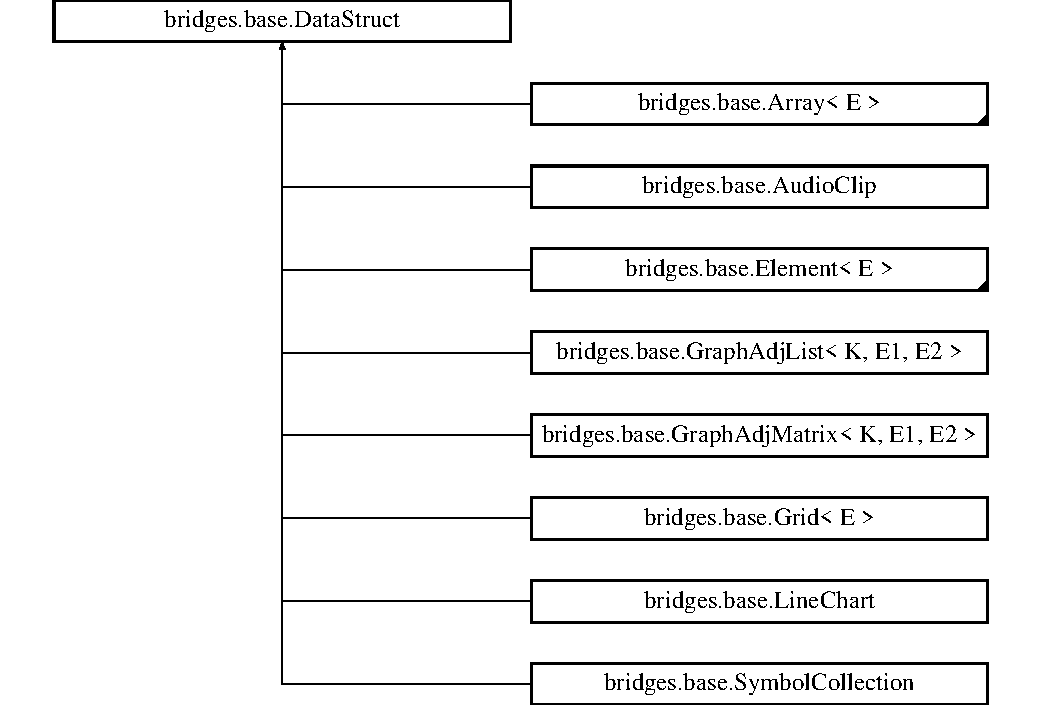
\includegraphics[height=3.485477cm]{classbridges_1_1base_1_1_data_struct}
\end{center}
\end{figure}
\subsection*{Protected Member Functions}
\begin{DoxyCompactItemize}
\item 
abstract String \hyperlink{classbridges_1_1base_1_1_data_struct_a3bae9d0d68a85e517a34be482e90fdd4}{get\+Data\+Struct\+Type} ()
\end{DoxyCompactItemize}
\subsection*{Protected Attributes}
\begin{DoxyCompactItemize}
\item 
String \hyperlink{classbridges_1_1base_1_1_data_struct_aac4a6ea28f44676274120ba1dddafc1f}{Q\+U\+O\+TE} = \char`\"{}\textbackslash{}\char`\"{}\char`\"{}
\end{DoxyCompactItemize}


\subsection{Detailed Description}
This is an abstract super class that is extended by all Bridges subclasses and provides some methods that are used universally across B\+R\+I\+D\+G\+ES. 

\subsection{Member Function Documentation}
\hypertarget{classbridges_1_1base_1_1_data_struct_a3bae9d0d68a85e517a34be482e90fdd4}{}\label{classbridges_1_1base_1_1_data_struct_a3bae9d0d68a85e517a34be482e90fdd4} 
\index{bridges\+::base\+::\+Data\+Struct@{bridges\+::base\+::\+Data\+Struct}!get\+Data\+Struct\+Type@{get\+Data\+Struct\+Type}}
\index{get\+Data\+Struct\+Type@{get\+Data\+Struct\+Type}!bridges\+::base\+::\+Data\+Struct@{bridges\+::base\+::\+Data\+Struct}}
\subsubsection{\texorpdfstring{get\+Data\+Struct\+Type()}{getDataStructType()}}
{\footnotesize\ttfamily abstract String bridges.\+base.\+Data\+Struct.\+get\+Data\+Struct\+Type (\begin{DoxyParamCaption}{ }\end{DoxyParamCaption})\hspace{0.3cm}{\ttfamily [abstract]}, {\ttfamily [protected]}}



\subsection{Member Data Documentation}
\hypertarget{classbridges_1_1base_1_1_data_struct_aac4a6ea28f44676274120ba1dddafc1f}{}\label{classbridges_1_1base_1_1_data_struct_aac4a6ea28f44676274120ba1dddafc1f} 
\index{bridges\+::base\+::\+Data\+Struct@{bridges\+::base\+::\+Data\+Struct}!Q\+U\+O\+TE@{Q\+U\+O\+TE}}
\index{Q\+U\+O\+TE@{Q\+U\+O\+TE}!bridges\+::base\+::\+Data\+Struct@{bridges\+::base\+::\+Data\+Struct}}
\subsubsection{\texorpdfstring{Q\+U\+O\+TE}{QUOTE}}
{\footnotesize\ttfamily String bridges.\+base.\+Data\+Struct.\+Q\+U\+O\+TE = \char`\"{}\textbackslash{}\char`\"{}\char`\"{}\hspace{0.3cm}{\ttfamily [protected]}}



The documentation for this class was generated from the following file\+:\begin{DoxyCompactItemize}
\item 
/\+Users/kalpathi/gr/bridges/client/java/bridges16/src/main/java/edu/uncc/cs/bridges\+\_\+v21/base/\hyperlink{_data_struct_8java}{Data\+Struct.\+java}\end{DoxyCompactItemize}

\hypertarget{classbridges_1_1base_1_1_d_lelement}{}\section{bridges.\+base.\+D\+Lelement$<$ E $>$ Class Template Reference}
\label{classbridges_1_1base_1_1_d_lelement}\index{bridges.\+base.\+D\+Lelement$<$ E $>$@{bridges.\+base.\+D\+Lelement$<$ E $>$}}


This class is used to create doubly linked element objects.  


Inheritance diagram for bridges.\+base.\+D\+Lelement$<$ E $>$\+:\begin{figure}[H]
\begin{center}
\leavevmode
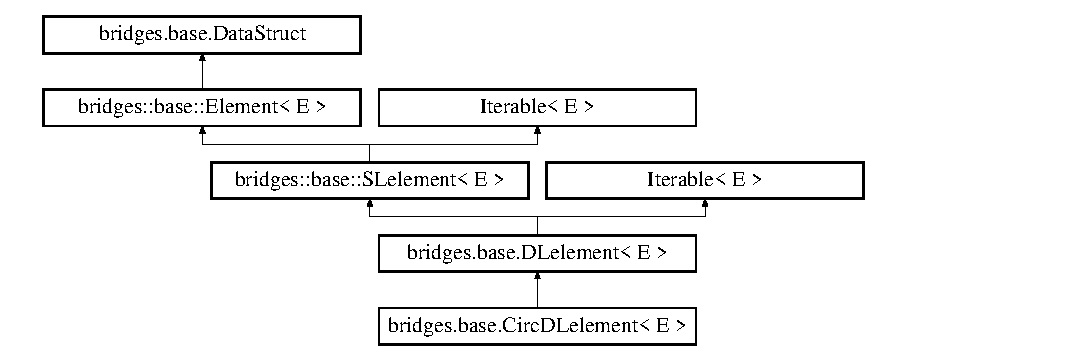
\includegraphics[height=5.000000cm]{classbridges_1_1base_1_1_d_lelement}
\end{center}
\end{figure}
\subsection*{Public Member Functions}
\begin{DoxyCompactItemize}
\item 
\hyperlink{classbridges_1_1base_1_1_d_lelement_a525b572340e161d9c430baff10b64ab2}{D\+Lelement} ()
\item 
\hyperlink{classbridges_1_1base_1_1_d_lelement_a6aa1d4a3dad4a196c2ed079d108562bc}{D\+Lelement} (String label, E e)
\item 
\hyperlink{classbridges_1_1base_1_1_d_lelement_ab1e4eace66bb1b097463c4f04e964cd0}{D\+Lelement} (\hyperlink{classbridges_1_1base_1_1_d_lelement}{D\+Lelement}$<$ E $>$ \hyperlink{classbridges_1_1base_1_1_s_lelement_abf61c96a74ad319d561c6952ea388e0e}{next}, \hyperlink{classbridges_1_1base_1_1_d_lelement}{D\+Lelement}$<$ E $>$ \hyperlink{classbridges_1_1base_1_1_d_lelement_a6eba4876f820b75ac6bde01d7dea9da7}{prev})
\item 
\hyperlink{classbridges_1_1base_1_1_d_lelement_a3ffba30204a2ea6939b07b0ded123af5}{D\+Lelement} (E e, \hyperlink{classbridges_1_1base_1_1_d_lelement}{D\+Lelement}$<$ E $>$ \hyperlink{classbridges_1_1base_1_1_s_lelement_abf61c96a74ad319d561c6952ea388e0e}{next}, \hyperlink{classbridges_1_1base_1_1_d_lelement}{D\+Lelement}$<$ E $>$ \hyperlink{classbridges_1_1base_1_1_d_lelement_a6eba4876f820b75ac6bde01d7dea9da7}{prev})
\item 
String \hyperlink{classbridges_1_1base_1_1_d_lelement_a4a0e8f7bd377a652927a741e70aae6d3}{get\+Data\+Struct\+Type} ()
\item 
\hyperlink{classbridges_1_1base_1_1_d_lelement}{D\+Lelement}$<$ E $>$ \hyperlink{classbridges_1_1base_1_1_d_lelement_a35e88e8d991d6f23ec63b3ef3f6cce4e}{get\+Next} ()
\item 
\hyperlink{classbridges_1_1base_1_1_d_lelement}{D\+Lelement}$<$ E $>$ \hyperlink{classbridges_1_1base_1_1_d_lelement_a859f08f38513ecdfff0eb11bd2b98ce7}{get\+Prev} ()
\item 
void \hyperlink{classbridges_1_1base_1_1_d_lelement_a152a06add922290d48b2d4affc87d592}{set\+Prev} (\hyperlink{classbridges_1_1base_1_1_d_lelement}{D\+Lelement}$<$ E $>$ prv)
\item 
String \hyperlink{classbridges_1_1base_1_1_d_lelement_aefe2e582992a9e574d733f109add80f2}{get\+Data\+Structure\+Representation} ()
\end{DoxyCompactItemize}
\subsection*{Protected Attributes}
\begin{DoxyCompactItemize}
\item 
\hyperlink{classbridges_1_1base_1_1_d_lelement}{D\+Lelement}$<$ E $>$ \hyperlink{classbridges_1_1base_1_1_d_lelement_a6eba4876f820b75ac6bde01d7dea9da7}{prev}
\end{DoxyCompactItemize}
\subsection*{Additional Inherited Members}


\subsection{Detailed Description}
This class is used to create doubly linked element objects. 

\begin{DoxyAuthor}{Author}
Mihai Mehedint, Kalpathi Subramanian
\end{DoxyAuthor}
\begin{DoxyDate}{Date}
6/22/16, 1/7/17, 5/17/17
\end{DoxyDate}
This class extends \hyperlink{classbridges_1_1base_1_1_element}{Element} and takes a generic parameter $<$\+E$>$ representing application specific data. This element forms the basic building block for doubly linked lists. Doubly linked elements have two links, \char`\"{}next\char`\"{} and \char`\"{}previous\char`\"{}, that point to the previous and succeeding nodes along the list.

Elements contain a visualizer (\hyperlink{classbridges_1_1base_1_1_element_visualizer}{Element\+Visualizer}) object for setting visual attributes (color, shape, opacity, size), necessary for displaying them in a web browser.

Elements also have a \hyperlink{classbridges_1_1base_1_1_link_visualizer}{Link\+Visualizer} object that is used when they are linked to another element, appropriate for setting link attributes, such as in linked lists, between the current element and its next or previous nodes.


\begin{DoxyParams}{Parameters}
{\em $<$\+E$>$} & The generic parameter object that is part of this element, representing application specific data.\\
\hline
\end{DoxyParams}
\begin{DoxySeeAlso}{See also}
Example Tutorial at ~\newline
 \href{http://bridgesuncc.github.io/Hello_World_Tutorials/DLL.html}{\tt http\+://bridgesuncc.\+github.\+io/\+Hello\+\_\+\+World\+\_\+\+Tutorials/\+D\+L\+L.\+html} 
\end{DoxySeeAlso}


\subsection{Constructor \& Destructor Documentation}
\hypertarget{classbridges_1_1base_1_1_d_lelement_a525b572340e161d9c430baff10b64ab2}{}\index{bridges\+::base\+::\+D\+Lelement@{bridges\+::base\+::\+D\+Lelement}!D\+Lelement@{D\+Lelement}}
\index{D\+Lelement@{D\+Lelement}!bridges\+::base\+::\+D\+Lelement@{bridges\+::base\+::\+D\+Lelement}}
\subsubsection[{D\+Lelement()}]{\setlength{\rightskip}{0pt plus 5cm}{\bf bridges.\+base.\+D\+Lelement}$<$ E $>$.{\bf D\+Lelement} (
\begin{DoxyParamCaption}
{}
\end{DoxyParamCaption}
)}\label{classbridges_1_1base_1_1_d_lelement_a525b572340e161d9c430baff10b64ab2}
Constructs an empty \hyperlink{classbridges_1_1base_1_1_d_lelement}{D\+Lelement} with next and prev pointers set to null. \hypertarget{classbridges_1_1base_1_1_d_lelement_a6aa1d4a3dad4a196c2ed079d108562bc}{}\index{bridges\+::base\+::\+D\+Lelement@{bridges\+::base\+::\+D\+Lelement}!D\+Lelement@{D\+Lelement}}
\index{D\+Lelement@{D\+Lelement}!bridges\+::base\+::\+D\+Lelement@{bridges\+::base\+::\+D\+Lelement}}
\subsubsection[{D\+Lelement(\+String label, E e)}]{\setlength{\rightskip}{0pt plus 5cm}{\bf bridges.\+base.\+D\+Lelement}$<$ E $>$.{\bf D\+Lelement} (
\begin{DoxyParamCaption}
\item[{String}]{label, }
\item[{E}]{e}
\end{DoxyParamCaption}
)}\label{classbridges_1_1base_1_1_d_lelement_a6aa1d4a3dad4a196c2ed079d108562bc}
Constructs a \hyperlink{classbridges_1_1base_1_1_d_lelement}{D\+Lelement} labeled \char`\"{}label\char`\"{}, holding an object \char`\"{}e\char`\"{}, with next and prev pointers set to null.


\begin{DoxyParams}{Parameters}
{\em label} & the label for this \hyperlink{classbridges_1_1base_1_1_d_lelement}{D\+Lelement} that shows up on the Bridges visualization \\
\hline
{\em e} & the genereic object that is held in this element. \\
\hline
\end{DoxyParams}
\hypertarget{classbridges_1_1base_1_1_d_lelement_ab1e4eace66bb1b097463c4f04e964cd0}{}\index{bridges\+::base\+::\+D\+Lelement@{bridges\+::base\+::\+D\+Lelement}!D\+Lelement@{D\+Lelement}}
\index{D\+Lelement@{D\+Lelement}!bridges\+::base\+::\+D\+Lelement@{bridges\+::base\+::\+D\+Lelement}}
\subsubsection[{D\+Lelement(\+D\+Lelement$<$ E $>$ next, D\+Lelement$<$ E $>$ prev)}]{\setlength{\rightskip}{0pt plus 5cm}{\bf bridges.\+base.\+D\+Lelement}$<$ E $>$.{\bf D\+Lelement} (
\begin{DoxyParamCaption}
\item[{{\bf D\+Lelement}$<$ E $>$}]{next, }
\item[{{\bf D\+Lelement}$<$ E $>$}]{prev}
\end{DoxyParamCaption}
)}\label{classbridges_1_1base_1_1_d_lelement_ab1e4eace66bb1b097463c4f04e964cd0}
Constructs an empty \hyperlink{classbridges_1_1base_1_1_d_lelement}{D\+Lelement} with the next pointer set to the \hyperlink{classbridges_1_1base_1_1_d_lelement}{D\+Lelement} \char`\"{}next\char`\"{} and the prev pointer set to \hyperlink{classbridges_1_1base_1_1_d_lelement}{D\+Lelement} \char`\"{}prev\char`\"{}.


\begin{DoxyParams}{Parameters}
{\em next} & the \hyperlink{classbridges_1_1base_1_1_d_lelement}{D\+Lelement} that should be assigned to the next pointer \\
\hline
{\em prev} & the \hyperlink{classbridges_1_1base_1_1_d_lelement}{D\+Lelement} that should be assigned to the prev pointer \\
\hline
\end{DoxyParams}
\hypertarget{classbridges_1_1base_1_1_d_lelement_a3ffba30204a2ea6939b07b0ded123af5}{}\index{bridges\+::base\+::\+D\+Lelement@{bridges\+::base\+::\+D\+Lelement}!D\+Lelement@{D\+Lelement}}
\index{D\+Lelement@{D\+Lelement}!bridges\+::base\+::\+D\+Lelement@{bridges\+::base\+::\+D\+Lelement}}
\subsubsection[{D\+Lelement(\+E e, D\+Lelement$<$ E $>$ next, D\+Lelement$<$ E $>$ prev)}]{\setlength{\rightskip}{0pt plus 5cm}{\bf bridges.\+base.\+D\+Lelement}$<$ E $>$.{\bf D\+Lelement} (
\begin{DoxyParamCaption}
\item[{E}]{e, }
\item[{{\bf D\+Lelement}$<$ E $>$}]{next, }
\item[{{\bf D\+Lelement}$<$ E $>$}]{prev}
\end{DoxyParamCaption}
)}\label{classbridges_1_1base_1_1_d_lelement_a3ffba30204a2ea6939b07b0ded123af5}
Constructs a \hyperlink{classbridges_1_1base_1_1_d_lelement}{D\+Lelement} holding an object \char`\"{}e\char`\"{}, with the next pointer set to the \hyperlink{classbridges_1_1base_1_1_d_lelement}{D\+Lelement} \char`\"{}next\char`\"{} and the prev pointer set to \hyperlink{classbridges_1_1base_1_1_d_lelement}{D\+Lelement} \char`\"{}prev\char`\"{}.


\begin{DoxyParams}{Parameters}
{\em e} & the genereic object that this \hyperlink{classbridges_1_1base_1_1_d_lelement}{D\+Lelement} is holding \\
\hline
{\em next} & the \hyperlink{classbridges_1_1base_1_1_d_lelement}{D\+Lelement} that should be assigned to the next pointer \\
\hline
{\em prev} & the \hyperlink{classbridges_1_1base_1_1_d_lelement}{D\+Lelement} that should be assigned to the prev pointer \\
\hline
\end{DoxyParams}


\subsection{Member Function Documentation}
\hypertarget{classbridges_1_1base_1_1_d_lelement_a4a0e8f7bd377a652927a741e70aae6d3}{}\index{bridges\+::base\+::\+D\+Lelement@{bridges\+::base\+::\+D\+Lelement}!get\+Data\+Struct\+Type@{get\+Data\+Struct\+Type}}
\index{get\+Data\+Struct\+Type@{get\+Data\+Struct\+Type}!bridges\+::base\+::\+D\+Lelement@{bridges\+::base\+::\+D\+Lelement}}
\subsubsection[{get\+Data\+Struct\+Type()}]{\setlength{\rightskip}{0pt plus 5cm}String {\bf bridges.\+base.\+D\+Lelement}$<$ E $>$.get\+Data\+Struct\+Type (
\begin{DoxyParamCaption}
{}
\end{DoxyParamCaption}
)}\label{classbridges_1_1base_1_1_d_lelement_a4a0e8f7bd377a652927a741e70aae6d3}
This method gets the data structure type

\begin{DoxyReturn}{Returns}
The date structure type as a string 
\end{DoxyReturn}
\hypertarget{classbridges_1_1base_1_1_d_lelement_aefe2e582992a9e574d733f109add80f2}{}\index{bridges\+::base\+::\+D\+Lelement@{bridges\+::base\+::\+D\+Lelement}!get\+Data\+Structure\+Representation@{get\+Data\+Structure\+Representation}}
\index{get\+Data\+Structure\+Representation@{get\+Data\+Structure\+Representation}!bridges\+::base\+::\+D\+Lelement@{bridges\+::base\+::\+D\+Lelement}}
\subsubsection[{get\+Data\+Structure\+Representation()}]{\setlength{\rightskip}{0pt plus 5cm}String {\bf bridges.\+base.\+D\+Lelement}$<$ E $>$.get\+Data\+Structure\+Representation (
\begin{DoxyParamCaption}
{}
\end{DoxyParamCaption}
)}\label{classbridges_1_1base_1_1_d_lelement_aefe2e582992a9e574d733f109add80f2}
\hypertarget{classbridges_1_1base_1_1_d_lelement_a35e88e8d991d6f23ec63b3ef3f6cce4e}{}\index{bridges\+::base\+::\+D\+Lelement@{bridges\+::base\+::\+D\+Lelement}!get\+Next@{get\+Next}}
\index{get\+Next@{get\+Next}!bridges\+::base\+::\+D\+Lelement@{bridges\+::base\+::\+D\+Lelement}}
\subsubsection[{get\+Next()}]{\setlength{\rightskip}{0pt plus 5cm}{\bf D\+Lelement}$<$E$>$ {\bf bridges.\+base.\+D\+Lelement}$<$ E $>$.get\+Next (
\begin{DoxyParamCaption}
{}
\end{DoxyParamCaption}
)}\label{classbridges_1_1base_1_1_d_lelement_a35e88e8d991d6f23ec63b3ef3f6cce4e}
This method returns the pointer to the next \hyperlink{classbridges_1_1base_1_1_d_lelement}{D\+Lelement}

\begin{DoxyReturn}{Returns}
the \hyperlink{classbridges_1_1base_1_1_d_lelement}{D\+Lelement} assigned to the next pointer 
\end{DoxyReturn}
\hypertarget{classbridges_1_1base_1_1_d_lelement_a859f08f38513ecdfff0eb11bd2b98ce7}{}\index{bridges\+::base\+::\+D\+Lelement@{bridges\+::base\+::\+D\+Lelement}!get\+Prev@{get\+Prev}}
\index{get\+Prev@{get\+Prev}!bridges\+::base\+::\+D\+Lelement@{bridges\+::base\+::\+D\+Lelement}}
\subsubsection[{get\+Prev()}]{\setlength{\rightskip}{0pt plus 5cm}{\bf D\+Lelement}$<$E$>$ {\bf bridges.\+base.\+D\+Lelement}$<$ E $>$.get\+Prev (
\begin{DoxyParamCaption}
{}
\end{DoxyParamCaption}
)}\label{classbridges_1_1base_1_1_d_lelement_a859f08f38513ecdfff0eb11bd2b98ce7}
This method sets the pointer to the next \hyperlink{classbridges_1_1base_1_1_d_lelement}{D\+Lelement}


\begin{DoxyParams}{Parameters}
{\em next} & the \hyperlink{classbridges_1_1base_1_1_d_lelement}{D\+Lelement} that should be assigned to the next pointer This method returns the pointer to the previous \hyperlink{classbridges_1_1base_1_1_d_lelement}{D\+Lelement}\\
\hline
\end{DoxyParams}
\begin{DoxyReturn}{Returns}
the \hyperlink{classbridges_1_1base_1_1_d_lelement}{D\+Lelement} assigned to the prev pointer 
\end{DoxyReturn}
\hypertarget{classbridges_1_1base_1_1_d_lelement_a152a06add922290d48b2d4affc87d592}{}\index{bridges\+::base\+::\+D\+Lelement@{bridges\+::base\+::\+D\+Lelement}!set\+Prev@{set\+Prev}}
\index{set\+Prev@{set\+Prev}!bridges\+::base\+::\+D\+Lelement@{bridges\+::base\+::\+D\+Lelement}}
\subsubsection[{set\+Prev(\+D\+Lelement$<$ E $>$ prv)}]{\setlength{\rightskip}{0pt plus 5cm}void {\bf bridges.\+base.\+D\+Lelement}$<$ E $>$.set\+Prev (
\begin{DoxyParamCaption}
\item[{{\bf D\+Lelement}$<$ E $>$}]{prv}
\end{DoxyParamCaption}
)}\label{classbridges_1_1base_1_1_d_lelement_a152a06add922290d48b2d4affc87d592}
This method sets the pointer to the previous \hyperlink{classbridges_1_1base_1_1_d_lelement}{D\+Lelement}


\begin{DoxyParams}{Parameters}
{\em prev} & the \hyperlink{classbridges_1_1base_1_1_d_lelement}{D\+Lelement} that should be assigned to the prev pointer \\
\hline
\end{DoxyParams}


\subsection{Member Data Documentation}
\hypertarget{classbridges_1_1base_1_1_d_lelement_a6eba4876f820b75ac6bde01d7dea9da7}{}\index{bridges\+::base\+::\+D\+Lelement@{bridges\+::base\+::\+D\+Lelement}!prev@{prev}}
\index{prev@{prev}!bridges\+::base\+::\+D\+Lelement@{bridges\+::base\+::\+D\+Lelement}}
\subsubsection[{prev}]{\setlength{\rightskip}{0pt plus 5cm}{\bf D\+Lelement}$<$E$>$ {\bf bridges.\+base.\+D\+Lelement}$<$ E $>$.prev\hspace{0.3cm}{\ttfamily [protected]}}\label{classbridges_1_1base_1_1_d_lelement_a6eba4876f820b75ac6bde01d7dea9da7}


The documentation for this class was generated from the following file\+:\begin{DoxyCompactItemize}
\item 
/\+Users/kalpathi/gr/bridges/bridges17/java/src/main/java/bridges/base/\hyperlink{_d_lelement_8java}{D\+Lelement.\+java}\end{DoxyCompactItemize}

\hypertarget{classbridges_1_1data__src__dependent_1_1_earthquake_u_s_g_s}{}\section{bridges.\+data\+\_\+src\+\_\+dependent.\+Earthquake\+U\+S\+G\+S Class Reference}
\label{classbridges_1_1data__src__dependent_1_1_earthquake_u_s_g_s}\index{bridges.\+data\+\_\+src\+\_\+dependent.\+Earthquake\+U\+S\+G\+S@{bridges.\+data\+\_\+src\+\_\+dependent.\+Earthquake\+U\+S\+G\+S}}
Inheritance diagram for bridges.\+data\+\_\+src\+\_\+dependent.\+Earthquake\+U\+S\+G\+S\+:\begin{figure}[H]
\begin{center}
\leavevmode
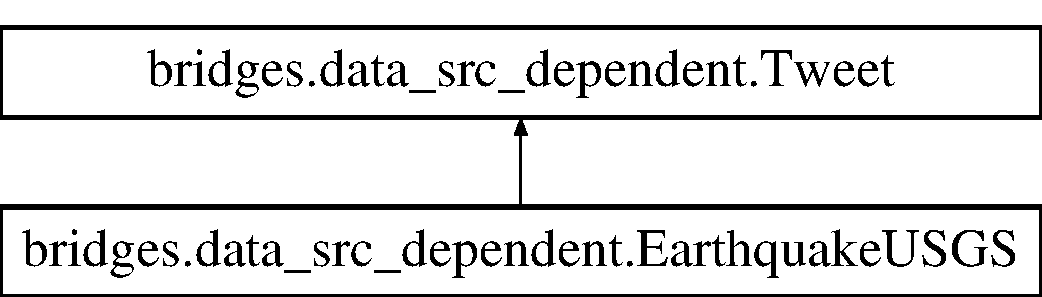
\includegraphics[height=2.000000cm]{classbridges_1_1data__src__dependent_1_1_earthquake_u_s_g_s}
\end{center}
\end{figure}
\subsection*{Public Member Functions}
\begin{DoxyCompactItemize}
\item 
\hyperlink{classbridges_1_1data__src__dependent_1_1_earthquake_u_s_g_s_a1803f7d357ce045cefbc923e096e9646}{Earthquake\+U\+S\+G\+S} ()
\item 
\hyperlink{classbridges_1_1data__src__dependent_1_1_earthquake_u_s_g_s_a767aa387d5ce45c98ad01394e0937abe}{Earthquake\+U\+S\+G\+S} (String content, Date date2, double magnitude, double longit, double latit, String location, String title, String url, String properties)
\item 
String \hyperlink{classbridges_1_1data__src__dependent_1_1_earthquake_u_s_g_s_a6676a3f0a11accf6a510648601e05310}{get\+Properties} ()
\item 
void \hyperlink{classbridges_1_1data__src__dependent_1_1_earthquake_u_s_g_s_a2e1ee813dc91081bbd8fd8f5b343f080}{set\+Properties} (String properties)
\item 
double \hyperlink{classbridges_1_1data__src__dependent_1_1_earthquake_u_s_g_s_a1b702f3081df4e29427fd4261fd57b42}{get\+Latit} ()
\item 
void \hyperlink{classbridges_1_1data__src__dependent_1_1_earthquake_u_s_g_s_aa8ca3a3aa511f52ba8bbae88118ede95}{set\+Latit} (double latit)
\item 
double \hyperlink{classbridges_1_1data__src__dependent_1_1_earthquake_u_s_g_s_a466f3594dfe3201ec468517067c3b3e5}{get\+Longit} ()
\item 
void \hyperlink{classbridges_1_1data__src__dependent_1_1_earthquake_u_s_g_s_a6e642131d91fb89bde4f13fe579f79c6}{set\+Longit} (double longit)
\item 
String \hyperlink{classbridges_1_1data__src__dependent_1_1_earthquake_u_s_g_s_a703492ad551b68ab6b7821646f9a92ec}{get\+Location} ()
\item 
void \hyperlink{classbridges_1_1data__src__dependent_1_1_earthquake_u_s_g_s_a473107844daa1ef938dd1b78e585185b}{set\+Location} (String location)
\item 
String \hyperlink{classbridges_1_1data__src__dependent_1_1_earthquake_u_s_g_s_a6aa71b4b565be3971c8d3dfae31cb6ed}{get\+Title} ()
\item 
void \hyperlink{classbridges_1_1data__src__dependent_1_1_earthquake_u_s_g_s_a0432f641e0089fc004c441b7239ad6a0}{set\+Title} (String title)
\item 
String \hyperlink{classbridges_1_1data__src__dependent_1_1_earthquake_u_s_g_s_a2af3938390c31096329e635510df437e}{get\+Url} ()
\item 
void \hyperlink{classbridges_1_1data__src__dependent_1_1_earthquake_u_s_g_s_aaa9d26333e7b80d0f72da58ea2ad41d1}{set\+Url} (String url)
\item 
void \hyperlink{classbridges_1_1data__src__dependent_1_1_earthquake_u_s_g_s_ad7902d80cbbe11046858db1f2792e99d}{set\+Magnitude} (double magnitude)
\item 
void \hyperlink{classbridges_1_1data__src__dependent_1_1_earthquake_u_s_g_s_ae3813930d3468eff007521f33c8e2139}{set\+Time} (String t)
\item 
String \hyperlink{classbridges_1_1data__src__dependent_1_1_earthquake_u_s_g_s_a03397a4410818546c5232f46a3d4ffc4}{get\+Time} ()
\item 
\hyperlink{classbridges_1_1data__src__dependent_1_1_earthquake_u_s_g_s_a6b9281a299d6e60736355eb8833f9e0d}{Earthquake\+U\+S\+G\+S} (\hyperlink{classbridges_1_1data__src__dependent_1_1_earthquake_u_s_g_s}{Earthquake\+U\+S\+G\+S} eq)
\item 
void \hyperlink{classbridges_1_1data__src__dependent_1_1_earthquake_u_s_g_s_acc0ba6890ee5963f88a399523f009ae4}{eq\+Properties} (String prop)
\item 
void \hyperlink{classbridges_1_1data__src__dependent_1_1_earthquake_u_s_g_s_a34a4c6ebe01c5daa7c86b3a4207d633f}{set\+Magnitude} (Double mag)
\item 
String \hyperlink{classbridges_1_1data__src__dependent_1_1_earthquake_u_s_g_s_aade0ce9a2fee927b015f5eb495c481e1}{enter\+Carriage\+Return} (String str)
\item 
double \hyperlink{classbridges_1_1data__src__dependent_1_1_earthquake_u_s_g_s_a3ec5d753277d6287b222448ff2477291}{get\+Magnitude} ()
\item 
int \hyperlink{classbridges_1_1data__src__dependent_1_1_earthquake_u_s_g_s_a60cad0a286825f77cd2900265acae982}{compare\+To} (Data\+Source o)
\end{DoxyCompactItemize}


\subsection{Detailed Description}
\begin{DoxyAuthor}{Author}
mihai mehedint 
\end{DoxyAuthor}


\subsection{Constructor \& Destructor Documentation}
\hypertarget{classbridges_1_1data__src__dependent_1_1_earthquake_u_s_g_s_a1803f7d357ce045cefbc923e096e9646}{}\index{bridges\+::data\+\_\+src\+\_\+dependent\+::\+Earthquake\+U\+S\+G\+S@{bridges\+::data\+\_\+src\+\_\+dependent\+::\+Earthquake\+U\+S\+G\+S}!Earthquake\+U\+S\+G\+S@{Earthquake\+U\+S\+G\+S}}
\index{Earthquake\+U\+S\+G\+S@{Earthquake\+U\+S\+G\+S}!bridges\+::data\+\_\+src\+\_\+dependent\+::\+Earthquake\+U\+S\+G\+S@{bridges\+::data\+\_\+src\+\_\+dependent\+::\+Earthquake\+U\+S\+G\+S}}
\subsubsection[{Earthquake\+U\+S\+G\+S()}]{\setlength{\rightskip}{0pt plus 5cm}bridges.\+data\+\_\+src\+\_\+dependent.\+Earthquake\+U\+S\+G\+S.\+Earthquake\+U\+S\+G\+S (
\begin{DoxyParamCaption}
{}
\end{DoxyParamCaption}
)}\label{classbridges_1_1data__src__dependent_1_1_earthquake_u_s_g_s_a1803f7d357ce045cefbc923e096e9646}
\hypertarget{classbridges_1_1data__src__dependent_1_1_earthquake_u_s_g_s_a767aa387d5ce45c98ad01394e0937abe}{}\index{bridges\+::data\+\_\+src\+\_\+dependent\+::\+Earthquake\+U\+S\+G\+S@{bridges\+::data\+\_\+src\+\_\+dependent\+::\+Earthquake\+U\+S\+G\+S}!Earthquake\+U\+S\+G\+S@{Earthquake\+U\+S\+G\+S}}
\index{Earthquake\+U\+S\+G\+S@{Earthquake\+U\+S\+G\+S}!bridges\+::data\+\_\+src\+\_\+dependent\+::\+Earthquake\+U\+S\+G\+S@{bridges\+::data\+\_\+src\+\_\+dependent\+::\+Earthquake\+U\+S\+G\+S}}
\subsubsection[{Earthquake\+U\+S\+G\+S(\+String content, Date date2, double magnitude, double longit, double latit, String location, String title, String url, String properties)}]{\setlength{\rightskip}{0pt plus 5cm}bridges.\+data\+\_\+src\+\_\+dependent.\+Earthquake\+U\+S\+G\+S.\+Earthquake\+U\+S\+G\+S (
\begin{DoxyParamCaption}
\item[{String}]{content, }
\item[{Date}]{date2, }
\item[{double}]{magnitude, }
\item[{double}]{longit, }
\item[{double}]{latit, }
\item[{String}]{location, }
\item[{String}]{title, }
\item[{String}]{url, }
\item[{String}]{properties}
\end{DoxyParamCaption}
)}\label{classbridges_1_1data__src__dependent_1_1_earthquake_u_s_g_s_a767aa387d5ce45c98ad01394e0937abe}
\hypertarget{classbridges_1_1data__src__dependent_1_1_earthquake_u_s_g_s_a6b9281a299d6e60736355eb8833f9e0d}{}\index{bridges\+::data\+\_\+src\+\_\+dependent\+::\+Earthquake\+U\+S\+G\+S@{bridges\+::data\+\_\+src\+\_\+dependent\+::\+Earthquake\+U\+S\+G\+S}!Earthquake\+U\+S\+G\+S@{Earthquake\+U\+S\+G\+S}}
\index{Earthquake\+U\+S\+G\+S@{Earthquake\+U\+S\+G\+S}!bridges\+::data\+\_\+src\+\_\+dependent\+::\+Earthquake\+U\+S\+G\+S@{bridges\+::data\+\_\+src\+\_\+dependent\+::\+Earthquake\+U\+S\+G\+S}}
\subsubsection[{Earthquake\+U\+S\+G\+S(\+Earthquake\+U\+S\+G\+S eq)}]{\setlength{\rightskip}{0pt plus 5cm}bridges.\+data\+\_\+src\+\_\+dependent.\+Earthquake\+U\+S\+G\+S.\+Earthquake\+U\+S\+G\+S (
\begin{DoxyParamCaption}
\item[{{\bf Earthquake\+U\+S\+G\+S}}]{eq}
\end{DoxyParamCaption}
)}\label{classbridges_1_1data__src__dependent_1_1_earthquake_u_s_g_s_a6b9281a299d6e60736355eb8833f9e0d}


\subsection{Member Function Documentation}
\hypertarget{classbridges_1_1data__src__dependent_1_1_earthquake_u_s_g_s_a60cad0a286825f77cd2900265acae982}{}\index{bridges\+::data\+\_\+src\+\_\+dependent\+::\+Earthquake\+U\+S\+G\+S@{bridges\+::data\+\_\+src\+\_\+dependent\+::\+Earthquake\+U\+S\+G\+S}!compare\+To@{compare\+To}}
\index{compare\+To@{compare\+To}!bridges\+::data\+\_\+src\+\_\+dependent\+::\+Earthquake\+U\+S\+G\+S@{bridges\+::data\+\_\+src\+\_\+dependent\+::\+Earthquake\+U\+S\+G\+S}}
\subsubsection[{compare\+To(\+Data\+Source o)}]{\setlength{\rightskip}{0pt plus 5cm}int bridges.\+data\+\_\+src\+\_\+dependent.\+Earthquake\+U\+S\+G\+S.\+compare\+To (
\begin{DoxyParamCaption}
\item[{Data\+Source}]{o}
\end{DoxyParamCaption}
)}\label{classbridges_1_1data__src__dependent_1_1_earthquake_u_s_g_s_a60cad0a286825f77cd2900265acae982}
\hypertarget{classbridges_1_1data__src__dependent_1_1_earthquake_u_s_g_s_aade0ce9a2fee927b015f5eb495c481e1}{}\index{bridges\+::data\+\_\+src\+\_\+dependent\+::\+Earthquake\+U\+S\+G\+S@{bridges\+::data\+\_\+src\+\_\+dependent\+::\+Earthquake\+U\+S\+G\+S}!enter\+Carriage\+Return@{enter\+Carriage\+Return}}
\index{enter\+Carriage\+Return@{enter\+Carriage\+Return}!bridges\+::data\+\_\+src\+\_\+dependent\+::\+Earthquake\+U\+S\+G\+S@{bridges\+::data\+\_\+src\+\_\+dependent\+::\+Earthquake\+U\+S\+G\+S}}
\subsubsection[{enter\+Carriage\+Return(\+String str)}]{\setlength{\rightskip}{0pt plus 5cm}String bridges.\+data\+\_\+src\+\_\+dependent.\+Earthquake\+U\+S\+G\+S.\+enter\+Carriage\+Return (
\begin{DoxyParamCaption}
\item[{String}]{str}
\end{DoxyParamCaption}
)}\label{classbridges_1_1data__src__dependent_1_1_earthquake_u_s_g_s_aade0ce9a2fee927b015f5eb495c481e1}
\hypertarget{classbridges_1_1data__src__dependent_1_1_earthquake_u_s_g_s_acc0ba6890ee5963f88a399523f009ae4}{}\index{bridges\+::data\+\_\+src\+\_\+dependent\+::\+Earthquake\+U\+S\+G\+S@{bridges\+::data\+\_\+src\+\_\+dependent\+::\+Earthquake\+U\+S\+G\+S}!eq\+Properties@{eq\+Properties}}
\index{eq\+Properties@{eq\+Properties}!bridges\+::data\+\_\+src\+\_\+dependent\+::\+Earthquake\+U\+S\+G\+S@{bridges\+::data\+\_\+src\+\_\+dependent\+::\+Earthquake\+U\+S\+G\+S}}
\subsubsection[{eq\+Properties(\+String prop)}]{\setlength{\rightskip}{0pt plus 5cm}void bridges.\+data\+\_\+src\+\_\+dependent.\+Earthquake\+U\+S\+G\+S.\+eq\+Properties (
\begin{DoxyParamCaption}
\item[{String}]{prop}
\end{DoxyParamCaption}
)}\label{classbridges_1_1data__src__dependent_1_1_earthquake_u_s_g_s_acc0ba6890ee5963f88a399523f009ae4}
\hypertarget{classbridges_1_1data__src__dependent_1_1_earthquake_u_s_g_s_a1b702f3081df4e29427fd4261fd57b42}{}\index{bridges\+::data\+\_\+src\+\_\+dependent\+::\+Earthquake\+U\+S\+G\+S@{bridges\+::data\+\_\+src\+\_\+dependent\+::\+Earthquake\+U\+S\+G\+S}!get\+Latit@{get\+Latit}}
\index{get\+Latit@{get\+Latit}!bridges\+::data\+\_\+src\+\_\+dependent\+::\+Earthquake\+U\+S\+G\+S@{bridges\+::data\+\_\+src\+\_\+dependent\+::\+Earthquake\+U\+S\+G\+S}}
\subsubsection[{get\+Latit()}]{\setlength{\rightskip}{0pt plus 5cm}double bridges.\+data\+\_\+src\+\_\+dependent.\+Earthquake\+U\+S\+G\+S.\+get\+Latit (
\begin{DoxyParamCaption}
{}
\end{DoxyParamCaption}
)}\label{classbridges_1_1data__src__dependent_1_1_earthquake_u_s_g_s_a1b702f3081df4e29427fd4261fd57b42}
\hypertarget{classbridges_1_1data__src__dependent_1_1_earthquake_u_s_g_s_a703492ad551b68ab6b7821646f9a92ec}{}\index{bridges\+::data\+\_\+src\+\_\+dependent\+::\+Earthquake\+U\+S\+G\+S@{bridges\+::data\+\_\+src\+\_\+dependent\+::\+Earthquake\+U\+S\+G\+S}!get\+Location@{get\+Location}}
\index{get\+Location@{get\+Location}!bridges\+::data\+\_\+src\+\_\+dependent\+::\+Earthquake\+U\+S\+G\+S@{bridges\+::data\+\_\+src\+\_\+dependent\+::\+Earthquake\+U\+S\+G\+S}}
\subsubsection[{get\+Location()}]{\setlength{\rightskip}{0pt plus 5cm}String bridges.\+data\+\_\+src\+\_\+dependent.\+Earthquake\+U\+S\+G\+S.\+get\+Location (
\begin{DoxyParamCaption}
{}
\end{DoxyParamCaption}
)}\label{classbridges_1_1data__src__dependent_1_1_earthquake_u_s_g_s_a703492ad551b68ab6b7821646f9a92ec}
\hypertarget{classbridges_1_1data__src__dependent_1_1_earthquake_u_s_g_s_a466f3594dfe3201ec468517067c3b3e5}{}\index{bridges\+::data\+\_\+src\+\_\+dependent\+::\+Earthquake\+U\+S\+G\+S@{bridges\+::data\+\_\+src\+\_\+dependent\+::\+Earthquake\+U\+S\+G\+S}!get\+Longit@{get\+Longit}}
\index{get\+Longit@{get\+Longit}!bridges\+::data\+\_\+src\+\_\+dependent\+::\+Earthquake\+U\+S\+G\+S@{bridges\+::data\+\_\+src\+\_\+dependent\+::\+Earthquake\+U\+S\+G\+S}}
\subsubsection[{get\+Longit()}]{\setlength{\rightskip}{0pt plus 5cm}double bridges.\+data\+\_\+src\+\_\+dependent.\+Earthquake\+U\+S\+G\+S.\+get\+Longit (
\begin{DoxyParamCaption}
{}
\end{DoxyParamCaption}
)}\label{classbridges_1_1data__src__dependent_1_1_earthquake_u_s_g_s_a466f3594dfe3201ec468517067c3b3e5}
\hypertarget{classbridges_1_1data__src__dependent_1_1_earthquake_u_s_g_s_a3ec5d753277d6287b222448ff2477291}{}\index{bridges\+::data\+\_\+src\+\_\+dependent\+::\+Earthquake\+U\+S\+G\+S@{bridges\+::data\+\_\+src\+\_\+dependent\+::\+Earthquake\+U\+S\+G\+S}!get\+Magnitude@{get\+Magnitude}}
\index{get\+Magnitude@{get\+Magnitude}!bridges\+::data\+\_\+src\+\_\+dependent\+::\+Earthquake\+U\+S\+G\+S@{bridges\+::data\+\_\+src\+\_\+dependent\+::\+Earthquake\+U\+S\+G\+S}}
\subsubsection[{get\+Magnitude()}]{\setlength{\rightskip}{0pt plus 5cm}double bridges.\+data\+\_\+src\+\_\+dependent.\+Earthquake\+U\+S\+G\+S.\+get\+Magnitude (
\begin{DoxyParamCaption}
{}
\end{DoxyParamCaption}
)}\label{classbridges_1_1data__src__dependent_1_1_earthquake_u_s_g_s_a3ec5d753277d6287b222448ff2477291}
\hypertarget{classbridges_1_1data__src__dependent_1_1_earthquake_u_s_g_s_a6676a3f0a11accf6a510648601e05310}{}\index{bridges\+::data\+\_\+src\+\_\+dependent\+::\+Earthquake\+U\+S\+G\+S@{bridges\+::data\+\_\+src\+\_\+dependent\+::\+Earthquake\+U\+S\+G\+S}!get\+Properties@{get\+Properties}}
\index{get\+Properties@{get\+Properties}!bridges\+::data\+\_\+src\+\_\+dependent\+::\+Earthquake\+U\+S\+G\+S@{bridges\+::data\+\_\+src\+\_\+dependent\+::\+Earthquake\+U\+S\+G\+S}}
\subsubsection[{get\+Properties()}]{\setlength{\rightskip}{0pt plus 5cm}String bridges.\+data\+\_\+src\+\_\+dependent.\+Earthquake\+U\+S\+G\+S.\+get\+Properties (
\begin{DoxyParamCaption}
{}
\end{DoxyParamCaption}
)}\label{classbridges_1_1data__src__dependent_1_1_earthquake_u_s_g_s_a6676a3f0a11accf6a510648601e05310}
\hypertarget{classbridges_1_1data__src__dependent_1_1_earthquake_u_s_g_s_a03397a4410818546c5232f46a3d4ffc4}{}\index{bridges\+::data\+\_\+src\+\_\+dependent\+::\+Earthquake\+U\+S\+G\+S@{bridges\+::data\+\_\+src\+\_\+dependent\+::\+Earthquake\+U\+S\+G\+S}!get\+Time@{get\+Time}}
\index{get\+Time@{get\+Time}!bridges\+::data\+\_\+src\+\_\+dependent\+::\+Earthquake\+U\+S\+G\+S@{bridges\+::data\+\_\+src\+\_\+dependent\+::\+Earthquake\+U\+S\+G\+S}}
\subsubsection[{get\+Time()}]{\setlength{\rightskip}{0pt plus 5cm}String bridges.\+data\+\_\+src\+\_\+dependent.\+Earthquake\+U\+S\+G\+S.\+get\+Time (
\begin{DoxyParamCaption}
{}
\end{DoxyParamCaption}
)}\label{classbridges_1_1data__src__dependent_1_1_earthquake_u_s_g_s_a03397a4410818546c5232f46a3d4ffc4}
\hypertarget{classbridges_1_1data__src__dependent_1_1_earthquake_u_s_g_s_a6aa71b4b565be3971c8d3dfae31cb6ed}{}\index{bridges\+::data\+\_\+src\+\_\+dependent\+::\+Earthquake\+U\+S\+G\+S@{bridges\+::data\+\_\+src\+\_\+dependent\+::\+Earthquake\+U\+S\+G\+S}!get\+Title@{get\+Title}}
\index{get\+Title@{get\+Title}!bridges\+::data\+\_\+src\+\_\+dependent\+::\+Earthquake\+U\+S\+G\+S@{bridges\+::data\+\_\+src\+\_\+dependent\+::\+Earthquake\+U\+S\+G\+S}}
\subsubsection[{get\+Title()}]{\setlength{\rightskip}{0pt plus 5cm}String bridges.\+data\+\_\+src\+\_\+dependent.\+Earthquake\+U\+S\+G\+S.\+get\+Title (
\begin{DoxyParamCaption}
{}
\end{DoxyParamCaption}
)}\label{classbridges_1_1data__src__dependent_1_1_earthquake_u_s_g_s_a6aa71b4b565be3971c8d3dfae31cb6ed}
\hypertarget{classbridges_1_1data__src__dependent_1_1_earthquake_u_s_g_s_a2af3938390c31096329e635510df437e}{}\index{bridges\+::data\+\_\+src\+\_\+dependent\+::\+Earthquake\+U\+S\+G\+S@{bridges\+::data\+\_\+src\+\_\+dependent\+::\+Earthquake\+U\+S\+G\+S}!get\+Url@{get\+Url}}
\index{get\+Url@{get\+Url}!bridges\+::data\+\_\+src\+\_\+dependent\+::\+Earthquake\+U\+S\+G\+S@{bridges\+::data\+\_\+src\+\_\+dependent\+::\+Earthquake\+U\+S\+G\+S}}
\subsubsection[{get\+Url()}]{\setlength{\rightskip}{0pt plus 5cm}String bridges.\+data\+\_\+src\+\_\+dependent.\+Earthquake\+U\+S\+G\+S.\+get\+Url (
\begin{DoxyParamCaption}
{}
\end{DoxyParamCaption}
)}\label{classbridges_1_1data__src__dependent_1_1_earthquake_u_s_g_s_a2af3938390c31096329e635510df437e}
\hypertarget{classbridges_1_1data__src__dependent_1_1_earthquake_u_s_g_s_aa8ca3a3aa511f52ba8bbae88118ede95}{}\index{bridges\+::data\+\_\+src\+\_\+dependent\+::\+Earthquake\+U\+S\+G\+S@{bridges\+::data\+\_\+src\+\_\+dependent\+::\+Earthquake\+U\+S\+G\+S}!set\+Latit@{set\+Latit}}
\index{set\+Latit@{set\+Latit}!bridges\+::data\+\_\+src\+\_\+dependent\+::\+Earthquake\+U\+S\+G\+S@{bridges\+::data\+\_\+src\+\_\+dependent\+::\+Earthquake\+U\+S\+G\+S}}
\subsubsection[{set\+Latit(double latit)}]{\setlength{\rightskip}{0pt plus 5cm}void bridges.\+data\+\_\+src\+\_\+dependent.\+Earthquake\+U\+S\+G\+S.\+set\+Latit (
\begin{DoxyParamCaption}
\item[{double}]{latit}
\end{DoxyParamCaption}
)}\label{classbridges_1_1data__src__dependent_1_1_earthquake_u_s_g_s_aa8ca3a3aa511f52ba8bbae88118ede95}
\hypertarget{classbridges_1_1data__src__dependent_1_1_earthquake_u_s_g_s_a473107844daa1ef938dd1b78e585185b}{}\index{bridges\+::data\+\_\+src\+\_\+dependent\+::\+Earthquake\+U\+S\+G\+S@{bridges\+::data\+\_\+src\+\_\+dependent\+::\+Earthquake\+U\+S\+G\+S}!set\+Location@{set\+Location}}
\index{set\+Location@{set\+Location}!bridges\+::data\+\_\+src\+\_\+dependent\+::\+Earthquake\+U\+S\+G\+S@{bridges\+::data\+\_\+src\+\_\+dependent\+::\+Earthquake\+U\+S\+G\+S}}
\subsubsection[{set\+Location(\+String location)}]{\setlength{\rightskip}{0pt plus 5cm}void bridges.\+data\+\_\+src\+\_\+dependent.\+Earthquake\+U\+S\+G\+S.\+set\+Location (
\begin{DoxyParamCaption}
\item[{String}]{location}
\end{DoxyParamCaption}
)}\label{classbridges_1_1data__src__dependent_1_1_earthquake_u_s_g_s_a473107844daa1ef938dd1b78e585185b}
\hypertarget{classbridges_1_1data__src__dependent_1_1_earthquake_u_s_g_s_a6e642131d91fb89bde4f13fe579f79c6}{}\index{bridges\+::data\+\_\+src\+\_\+dependent\+::\+Earthquake\+U\+S\+G\+S@{bridges\+::data\+\_\+src\+\_\+dependent\+::\+Earthquake\+U\+S\+G\+S}!set\+Longit@{set\+Longit}}
\index{set\+Longit@{set\+Longit}!bridges\+::data\+\_\+src\+\_\+dependent\+::\+Earthquake\+U\+S\+G\+S@{bridges\+::data\+\_\+src\+\_\+dependent\+::\+Earthquake\+U\+S\+G\+S}}
\subsubsection[{set\+Longit(double longit)}]{\setlength{\rightskip}{0pt plus 5cm}void bridges.\+data\+\_\+src\+\_\+dependent.\+Earthquake\+U\+S\+G\+S.\+set\+Longit (
\begin{DoxyParamCaption}
\item[{double}]{longit}
\end{DoxyParamCaption}
)}\label{classbridges_1_1data__src__dependent_1_1_earthquake_u_s_g_s_a6e642131d91fb89bde4f13fe579f79c6}
\hypertarget{classbridges_1_1data__src__dependent_1_1_earthquake_u_s_g_s_ad7902d80cbbe11046858db1f2792e99d}{}\index{bridges\+::data\+\_\+src\+\_\+dependent\+::\+Earthquake\+U\+S\+G\+S@{bridges\+::data\+\_\+src\+\_\+dependent\+::\+Earthquake\+U\+S\+G\+S}!set\+Magnitude@{set\+Magnitude}}
\index{set\+Magnitude@{set\+Magnitude}!bridges\+::data\+\_\+src\+\_\+dependent\+::\+Earthquake\+U\+S\+G\+S@{bridges\+::data\+\_\+src\+\_\+dependent\+::\+Earthquake\+U\+S\+G\+S}}
\subsubsection[{set\+Magnitude(double magnitude)}]{\setlength{\rightskip}{0pt plus 5cm}void bridges.\+data\+\_\+src\+\_\+dependent.\+Earthquake\+U\+S\+G\+S.\+set\+Magnitude (
\begin{DoxyParamCaption}
\item[{double}]{magnitude}
\end{DoxyParamCaption}
)}\label{classbridges_1_1data__src__dependent_1_1_earthquake_u_s_g_s_ad7902d80cbbe11046858db1f2792e99d}
\hypertarget{classbridges_1_1data__src__dependent_1_1_earthquake_u_s_g_s_a34a4c6ebe01c5daa7c86b3a4207d633f}{}\index{bridges\+::data\+\_\+src\+\_\+dependent\+::\+Earthquake\+U\+S\+G\+S@{bridges\+::data\+\_\+src\+\_\+dependent\+::\+Earthquake\+U\+S\+G\+S}!set\+Magnitude@{set\+Magnitude}}
\index{set\+Magnitude@{set\+Magnitude}!bridges\+::data\+\_\+src\+\_\+dependent\+::\+Earthquake\+U\+S\+G\+S@{bridges\+::data\+\_\+src\+\_\+dependent\+::\+Earthquake\+U\+S\+G\+S}}
\subsubsection[{set\+Magnitude(\+Double mag)}]{\setlength{\rightskip}{0pt plus 5cm}void bridges.\+data\+\_\+src\+\_\+dependent.\+Earthquake\+U\+S\+G\+S.\+set\+Magnitude (
\begin{DoxyParamCaption}
\item[{Double}]{mag}
\end{DoxyParamCaption}
)}\label{classbridges_1_1data__src__dependent_1_1_earthquake_u_s_g_s_a34a4c6ebe01c5daa7c86b3a4207d633f}
\hypertarget{classbridges_1_1data__src__dependent_1_1_earthquake_u_s_g_s_a2e1ee813dc91081bbd8fd8f5b343f080}{}\index{bridges\+::data\+\_\+src\+\_\+dependent\+::\+Earthquake\+U\+S\+G\+S@{bridges\+::data\+\_\+src\+\_\+dependent\+::\+Earthquake\+U\+S\+G\+S}!set\+Properties@{set\+Properties}}
\index{set\+Properties@{set\+Properties}!bridges\+::data\+\_\+src\+\_\+dependent\+::\+Earthquake\+U\+S\+G\+S@{bridges\+::data\+\_\+src\+\_\+dependent\+::\+Earthquake\+U\+S\+G\+S}}
\subsubsection[{set\+Properties(\+String properties)}]{\setlength{\rightskip}{0pt plus 5cm}void bridges.\+data\+\_\+src\+\_\+dependent.\+Earthquake\+U\+S\+G\+S.\+set\+Properties (
\begin{DoxyParamCaption}
\item[{String}]{properties}
\end{DoxyParamCaption}
)}\label{classbridges_1_1data__src__dependent_1_1_earthquake_u_s_g_s_a2e1ee813dc91081bbd8fd8f5b343f080}
\hypertarget{classbridges_1_1data__src__dependent_1_1_earthquake_u_s_g_s_ae3813930d3468eff007521f33c8e2139}{}\index{bridges\+::data\+\_\+src\+\_\+dependent\+::\+Earthquake\+U\+S\+G\+S@{bridges\+::data\+\_\+src\+\_\+dependent\+::\+Earthquake\+U\+S\+G\+S}!set\+Time@{set\+Time}}
\index{set\+Time@{set\+Time}!bridges\+::data\+\_\+src\+\_\+dependent\+::\+Earthquake\+U\+S\+G\+S@{bridges\+::data\+\_\+src\+\_\+dependent\+::\+Earthquake\+U\+S\+G\+S}}
\subsubsection[{set\+Time(\+String t)}]{\setlength{\rightskip}{0pt plus 5cm}void bridges.\+data\+\_\+src\+\_\+dependent.\+Earthquake\+U\+S\+G\+S.\+set\+Time (
\begin{DoxyParamCaption}
\item[{String}]{t}
\end{DoxyParamCaption}
)}\label{classbridges_1_1data__src__dependent_1_1_earthquake_u_s_g_s_ae3813930d3468eff007521f33c8e2139}
\hypertarget{classbridges_1_1data__src__dependent_1_1_earthquake_u_s_g_s_a0432f641e0089fc004c441b7239ad6a0}{}\index{bridges\+::data\+\_\+src\+\_\+dependent\+::\+Earthquake\+U\+S\+G\+S@{bridges\+::data\+\_\+src\+\_\+dependent\+::\+Earthquake\+U\+S\+G\+S}!set\+Title@{set\+Title}}
\index{set\+Title@{set\+Title}!bridges\+::data\+\_\+src\+\_\+dependent\+::\+Earthquake\+U\+S\+G\+S@{bridges\+::data\+\_\+src\+\_\+dependent\+::\+Earthquake\+U\+S\+G\+S}}
\subsubsection[{set\+Title(\+String title)}]{\setlength{\rightskip}{0pt plus 5cm}void bridges.\+data\+\_\+src\+\_\+dependent.\+Earthquake\+U\+S\+G\+S.\+set\+Title (
\begin{DoxyParamCaption}
\item[{String}]{title}
\end{DoxyParamCaption}
)}\label{classbridges_1_1data__src__dependent_1_1_earthquake_u_s_g_s_a0432f641e0089fc004c441b7239ad6a0}
\hypertarget{classbridges_1_1data__src__dependent_1_1_earthquake_u_s_g_s_aaa9d26333e7b80d0f72da58ea2ad41d1}{}\index{bridges\+::data\+\_\+src\+\_\+dependent\+::\+Earthquake\+U\+S\+G\+S@{bridges\+::data\+\_\+src\+\_\+dependent\+::\+Earthquake\+U\+S\+G\+S}!set\+Url@{set\+Url}}
\index{set\+Url@{set\+Url}!bridges\+::data\+\_\+src\+\_\+dependent\+::\+Earthquake\+U\+S\+G\+S@{bridges\+::data\+\_\+src\+\_\+dependent\+::\+Earthquake\+U\+S\+G\+S}}
\subsubsection[{set\+Url(\+String url)}]{\setlength{\rightskip}{0pt plus 5cm}void bridges.\+data\+\_\+src\+\_\+dependent.\+Earthquake\+U\+S\+G\+S.\+set\+Url (
\begin{DoxyParamCaption}
\item[{String}]{url}
\end{DoxyParamCaption}
)}\label{classbridges_1_1data__src__dependent_1_1_earthquake_u_s_g_s_aaa9d26333e7b80d0f72da58ea2ad41d1}


The documentation for this class was generated from the following file\+:\begin{DoxyCompactItemize}
\item 
/\+Users/kalpathi/gr/bridges/bridges17/java/src/main/java/bridges/data\+\_\+src\+\_\+dependent/\hyperlink{_earthquake_u_s_g_s_8java}{Earthquake\+U\+S\+G\+S.\+java}\end{DoxyCompactItemize}

\hypertarget{classbridges_1_1base_1_1_edge}{}\section{bridges.\+base.\+Edge$<$ K, E2 $>$ Class Template Reference}
\label{classbridges_1_1base_1_1_edge}\index{bridges.base.Edge$<$ K, E2 $>$@{bridges.base.Edge$<$ K, E2 $>$}}


This class is used to represent the edges in a graph and will appear as links in the B\+R\+I\+D\+G\+ES graph visualization.  


\subsection*{Public Member Functions}
\begin{DoxyCompactItemize}
\item 
\mbox{\hyperlink{classbridges_1_1base_1_1_edge_a2a17f458612fbcee8e9efb8d91a6cc18}{Edge}} (K from, K to, E2 data, \mbox{\hyperlink{classbridges_1_1base_1_1_link_visualizer}{Link\+Visualizer}} lvis)
\item 
void \mbox{\hyperlink{classbridges_1_1base_1_1_edge_aef1a55d996fc36217629b884435b9f35}{set\+From}} (K from)
\item 
void \mbox{\hyperlink{classbridges_1_1base_1_1_edge_a5e574139711be3f96c42da02a2702aea}{set\+To}} (K to)
\item 
K \mbox{\hyperlink{classbridges_1_1base_1_1_edge_ab451c13aa8173b5ef1cc2b2dd4f8508f}{get\+To}} ()
\item 
K \mbox{\hyperlink{classbridges_1_1base_1_1_edge_afc23a7c2ee8ab4c4f0950c9bf25edd56}{get\+From}} ()
\item 
void \mbox{\hyperlink{classbridges_1_1base_1_1_edge_a733d7f5eb4950d1fc4e14b7096faeb5c}{set\+Edge\+Data}} (E2 data)
\item 
E2 \mbox{\hyperlink{classbridges_1_1base_1_1_edge_a19a623d647eb17b7e53f1360577b0703}{get\+Edge\+Data}} ()
\item 
\mbox{\hyperlink{classbridges_1_1base_1_1_link_visualizer}{Link\+Visualizer}} \mbox{\hyperlink{classbridges_1_1base_1_1_edge_a11c655622b8a54f2931f59b1d256f84a}{get\+Link\+Visualizer}} ()
\item 
void \mbox{\hyperlink{classbridges_1_1base_1_1_edge_a1bb8008507d26245468bf9d0f1452072}{set\+Link\+Visualizer}} (\mbox{\hyperlink{classbridges_1_1base_1_1_link_visualizer}{Link\+Visualizer}} lvis)
\item 
String \mbox{\hyperlink{classbridges_1_1base_1_1_edge_a8663708d930e8df460c57d8bdbab44b2}{get\+Label}} ()
\item 
void \mbox{\hyperlink{classbridges_1_1base_1_1_edge_ad5f1d55a3c8caeb975f497dfe4f29242}{set\+Label}} (String label)
\item 
double \mbox{\hyperlink{classbridges_1_1base_1_1_edge_a3431e83235fc5d5dd5cf747ed4853881}{get\+Thickness}} ()
\item 
void \mbox{\hyperlink{classbridges_1_1base_1_1_edge_ae8d87539f03f04479e5f5710ea9bf260}{set\+Thickness}} (double thickness)
\item 
\mbox{\hyperlink{classbridges_1_1base_1_1_color}{Color}} \mbox{\hyperlink{classbridges_1_1base_1_1_edge_a243d9e6a57ebb570dda81bffe0cd4b77}{get\+Color}} ()
\item 
void \mbox{\hyperlink{classbridges_1_1base_1_1_edge_a77f6d36e94a3cbb8e478c85a1a6dad84}{set\+Color}} (\mbox{\hyperlink{classbridges_1_1base_1_1_color}{Color}} color)
\item 
void \mbox{\hyperlink{classbridges_1_1base_1_1_edge_adc2dbd9f8d74f8749ba64515ca052909}{set\+Color}} (String color)
\item 
void \mbox{\hyperlink{classbridges_1_1base_1_1_edge_a4ecf6bdaf140202b41c8a929fbdcdc0c}{set\+Color}} (int r, int g, int b, float a)
\end{DoxyCompactItemize}


\subsection{Detailed Description}
This class is used to represent the edges in a graph and will appear as links in the B\+R\+I\+D\+G\+ES graph visualization. 

This object is used in graphs and graph algorithms such as D\+FS, B\+FS and shortest path algorithms that need to visit graph edges. The adjacency list representation uses them as the generic paramter, as S\+Lelement$<$\+Edge$>$ Bridges represents Edges as links between pairs of elements

\begin{DoxyAuthor}{Author}
K.\+R. Subramanian
\end{DoxyAuthor}

\begin{DoxyParams}{Parameters}
{\em generic} & parameter $<$\+K$>$ holds the terminating vertex of the edge \\
\hline
{\em generic} & parameter $<$\+E2$>$ holds edge specific information \\
\hline
\end{DoxyParams}


\subsection{Constructor \& Destructor Documentation}
\mbox{\Hypertarget{classbridges_1_1base_1_1_edge_a2a17f458612fbcee8e9efb8d91a6cc18}\label{classbridges_1_1base_1_1_edge_a2a17f458612fbcee8e9efb8d91a6cc18}} 
\index{bridges.base.Edge$<$ K, E2 $>$@{bridges.base.Edge$<$ K, E2 $>$}!Edge@{Edge}}
\index{Edge@{Edge}!bridges.base.Edge$<$ K, E2 $>$@{bridges.base.Edge$<$ K, E2 $>$}}
\subsubsection{\texorpdfstring{Edge()}{Edge()}}
{\footnotesize\ttfamily \mbox{\hyperlink{classbridges_1_1base_1_1_edge}{bridges.\+base.\+Edge}}$<$ K, E2 $>$.\mbox{\hyperlink{classbridges_1_1base_1_1_edge}{Edge}} (\begin{DoxyParamCaption}\item[{K}]{from,  }\item[{K}]{to,  }\item[{E2}]{data,  }\item[{\mbox{\hyperlink{classbridges_1_1base_1_1_link_visualizer}{Link\+Visualizer}}}]{lvis }\end{DoxyParamCaption})}

Construct an edge with weight \char`\"{}wt\char`\"{} and a terminating \mbox{\hyperlink{classbridges_1_1base_1_1_element}{Element}} with an identifer equal to \char`\"{}v\char`\"{} -\/ used only for graphs


\begin{DoxyParams}{Parameters}
{\em from} & key of source vertex \\
\hline
{\em to} & ket of terminating vertex of the edge \\
\hline
{\em data} & is the edge information object \\
\hline
\end{DoxyParams}


\subsection{Member Function Documentation}
\mbox{\Hypertarget{classbridges_1_1base_1_1_edge_a243d9e6a57ebb570dda81bffe0cd4b77}\label{classbridges_1_1base_1_1_edge_a243d9e6a57ebb570dda81bffe0cd4b77}} 
\index{bridges.base.Edge$<$ K, E2 $>$@{bridges.base.Edge$<$ K, E2 $>$}!getColor@{getColor}}
\index{getColor@{getColor}!bridges.base.Edge$<$ K, E2 $>$@{bridges.base.Edge$<$ K, E2 $>$}}
\subsubsection{\texorpdfstring{getColor()}{getColor()}}
{\footnotesize\ttfamily \mbox{\hyperlink{classbridges_1_1base_1_1_color}{Color}} \mbox{\hyperlink{classbridges_1_1base_1_1_edge}{bridges.\+base.\+Edge}}$<$ K, E2 $>$.get\+Color (\begin{DoxyParamCaption}{ }\end{DoxyParamCaption})}

Get the color of the link in the Bridges Visualization

\begin{DoxyReturn}{Returns}
the \mbox{\hyperlink{classbridges_1_1base_1_1_color}{Color}} object representing the color of the link 
\end{DoxyReturn}
\mbox{\Hypertarget{classbridges_1_1base_1_1_edge_a19a623d647eb17b7e53f1360577b0703}\label{classbridges_1_1base_1_1_edge_a19a623d647eb17b7e53f1360577b0703}} 
\index{bridges.base.Edge$<$ K, E2 $>$@{bridges.base.Edge$<$ K, E2 $>$}!getEdgeData@{getEdgeData}}
\index{getEdgeData@{getEdgeData}!bridges.base.Edge$<$ K, E2 $>$@{bridges.base.Edge$<$ K, E2 $>$}}
\subsubsection{\texorpdfstring{getEdgeData()}{getEdgeData()}}
{\footnotesize\ttfamily E2 \mbox{\hyperlink{classbridges_1_1base_1_1_edge}{bridges.\+base.\+Edge}}$<$ K, E2 $>$.get\+Edge\+Data (\begin{DoxyParamCaption}{ }\end{DoxyParamCaption})}

Get edge specific data.

\begin{DoxyReturn}{Returns}
edge data 
\end{DoxyReturn}
\mbox{\Hypertarget{classbridges_1_1base_1_1_edge_afc23a7c2ee8ab4c4f0950c9bf25edd56}\label{classbridges_1_1base_1_1_edge_afc23a7c2ee8ab4c4f0950c9bf25edd56}} 
\index{bridges.base.Edge$<$ K, E2 $>$@{bridges.base.Edge$<$ K, E2 $>$}!getFrom@{getFrom}}
\index{getFrom@{getFrom}!bridges.base.Edge$<$ K, E2 $>$@{bridges.base.Edge$<$ K, E2 $>$}}
\subsubsection{\texorpdfstring{getFrom()}{getFrom()}}
{\footnotesize\ttfamily K \mbox{\hyperlink{classbridges_1_1base_1_1_edge}{bridges.\+base.\+Edge}}$<$ K, E2 $>$.get\+From (\begin{DoxyParamCaption}{ }\end{DoxyParamCaption})}

Get identifer of the source \mbox{\hyperlink{classbridges_1_1base_1_1_element}{Element}} of edge

\begin{DoxyReturn}{Returns}
the string identifier of the source \mbox{\hyperlink{classbridges_1_1base_1_1_element}{Element}} 
\end{DoxyReturn}
\mbox{\Hypertarget{classbridges_1_1base_1_1_edge_a8663708d930e8df460c57d8bdbab44b2}\label{classbridges_1_1base_1_1_edge_a8663708d930e8df460c57d8bdbab44b2}} 
\index{bridges.base.Edge$<$ K, E2 $>$@{bridges.base.Edge$<$ K, E2 $>$}!getLabel@{getLabel}}
\index{getLabel@{getLabel}!bridges.base.Edge$<$ K, E2 $>$@{bridges.base.Edge$<$ K, E2 $>$}}
\subsubsection{\texorpdfstring{getLabel()}{getLabel()}}
{\footnotesize\ttfamily String \mbox{\hyperlink{classbridges_1_1base_1_1_edge}{bridges.\+base.\+Edge}}$<$ K, E2 $>$.get\+Label (\begin{DoxyParamCaption}{ }\end{DoxyParamCaption})}

\mbox{\Hypertarget{classbridges_1_1base_1_1_edge_a11c655622b8a54f2931f59b1d256f84a}\label{classbridges_1_1base_1_1_edge_a11c655622b8a54f2931f59b1d256f84a}} 
\index{bridges.base.Edge$<$ K, E2 $>$@{bridges.base.Edge$<$ K, E2 $>$}!getLinkVisualizer@{getLinkVisualizer}}
\index{getLinkVisualizer@{getLinkVisualizer}!bridges.base.Edge$<$ K, E2 $>$@{bridges.base.Edge$<$ K, E2 $>$}}
\subsubsection{\texorpdfstring{getLinkVisualizer()}{getLinkVisualizer()}}
{\footnotesize\ttfamily \mbox{\hyperlink{classbridges_1_1base_1_1_link_visualizer}{Link\+Visualizer}} \mbox{\hyperlink{classbridges_1_1base_1_1_edge}{bridges.\+base.\+Edge}}$<$ K, E2 $>$.get\+Link\+Visualizer (\begin{DoxyParamCaption}{ }\end{DoxyParamCaption})}

\mbox{\Hypertarget{classbridges_1_1base_1_1_edge_a3431e83235fc5d5dd5cf747ed4853881}\label{classbridges_1_1base_1_1_edge_a3431e83235fc5d5dd5cf747ed4853881}} 
\index{bridges.base.Edge$<$ K, E2 $>$@{bridges.base.Edge$<$ K, E2 $>$}!getThickness@{getThickness}}
\index{getThickness@{getThickness}!bridges.base.Edge$<$ K, E2 $>$@{bridges.base.Edge$<$ K, E2 $>$}}
\subsubsection{\texorpdfstring{getThickness()}{getThickness()}}
{\footnotesize\ttfamily double \mbox{\hyperlink{classbridges_1_1base_1_1_edge}{bridges.\+base.\+Edge}}$<$ K, E2 $>$.get\+Thickness (\begin{DoxyParamCaption}{ }\end{DoxyParamCaption})}

Get the thickness of the link in the Bridges Visualiation

\begin{DoxyReturn}{Returns}
the size in pixels of the \mbox{\hyperlink{classbridges_1_1base_1_1_element}{Element}} in the Bridges Visualization 
\end{DoxyReturn}
\mbox{\Hypertarget{classbridges_1_1base_1_1_edge_ab451c13aa8173b5ef1cc2b2dd4f8508f}\label{classbridges_1_1base_1_1_edge_ab451c13aa8173b5ef1cc2b2dd4f8508f}} 
\index{bridges.base.Edge$<$ K, E2 $>$@{bridges.base.Edge$<$ K, E2 $>$}!getTo@{getTo}}
\index{getTo@{getTo}!bridges.base.Edge$<$ K, E2 $>$@{bridges.base.Edge$<$ K, E2 $>$}}
\subsubsection{\texorpdfstring{getTo()}{getTo()}}
{\footnotesize\ttfamily K \mbox{\hyperlink{classbridges_1_1base_1_1_edge}{bridges.\+base.\+Edge}}$<$ K, E2 $>$.get\+To (\begin{DoxyParamCaption}{ }\end{DoxyParamCaption})}

Get identifer of the terminating \mbox{\hyperlink{classbridges_1_1base_1_1_element}{Element}} of edge

\begin{DoxyReturn}{Returns}
the string identifier of the terminating \mbox{\hyperlink{classbridges_1_1base_1_1_element}{Element}} 
\end{DoxyReturn}
\mbox{\Hypertarget{classbridges_1_1base_1_1_edge_a77f6d36e94a3cbb8e478c85a1a6dad84}\label{classbridges_1_1base_1_1_edge_a77f6d36e94a3cbb8e478c85a1a6dad84}} 
\index{bridges.base.Edge$<$ K, E2 $>$@{bridges.base.Edge$<$ K, E2 $>$}!setColor@{setColor}}
\index{setColor@{setColor}!bridges.base.Edge$<$ K, E2 $>$@{bridges.base.Edge$<$ K, E2 $>$}}
\subsubsection{\texorpdfstring{setColor()}{setColor()}\hspace{0.1cm}{\footnotesize\ttfamily [1/3]}}
{\footnotesize\ttfamily void \mbox{\hyperlink{classbridges_1_1base_1_1_edge}{bridges.\+base.\+Edge}}$<$ K, E2 $>$.set\+Color (\begin{DoxyParamCaption}\item[{\mbox{\hyperlink{classbridges_1_1base_1_1_color}{Color}}}]{color }\end{DoxyParamCaption})}

Set the color of the link from an existing \mbox{\hyperlink{classbridges_1_1base_1_1_color}{Color}} object 
\begin{DoxyParams}{Parameters}
{\em color} & Bridges \mbox{\hyperlink{classbridges_1_1base_1_1_color}{Color}} object \\
\hline
\end{DoxyParams}
\mbox{\Hypertarget{classbridges_1_1base_1_1_edge_adc2dbd9f8d74f8749ba64515ca052909}\label{classbridges_1_1base_1_1_edge_adc2dbd9f8d74f8749ba64515ca052909}} 
\index{bridges.base.Edge$<$ K, E2 $>$@{bridges.base.Edge$<$ K, E2 $>$}!setColor@{setColor}}
\index{setColor@{setColor}!bridges.base.Edge$<$ K, E2 $>$@{bridges.base.Edge$<$ K, E2 $>$}}
\subsubsection{\texorpdfstring{setColor()}{setColor()}\hspace{0.1cm}{\footnotesize\ttfamily [2/3]}}
{\footnotesize\ttfamily void \mbox{\hyperlink{classbridges_1_1base_1_1_edge}{bridges.\+base.\+Edge}}$<$ K, E2 $>$.set\+Color (\begin{DoxyParamCaption}\item[{String}]{color }\end{DoxyParamCaption})}

Set the color of the link in the Bridges Visualization to \char`\"{}a\+Color\char`\"{}.


\begin{DoxyParams}{Parameters}
{\em col\+\_\+name} & the string reprsenting the color of the \mbox{\hyperlink{classbridges_1_1base_1_1_element}{Element}} in the Bridges Visualization; supported named colors are \char`\"{}red\char`\"{}, \char`\"{}green\char`\"{}, \char`\"{}blue\char`\"{}, \char`\"{}yellow\char`\"{}, \char`\"{}cyan\char`\"{}, \char`\"{}magenta\char`\"{}, \char`\"{}white\char`\"{}, \char`\"{}black\char`\"{}, \char`\"{}orange\char`\"{}, \char`\"{}turquoise\char`\"{}, \char`\"{}maroon\char`\"{}, \char`\"{}aquamarine\char`\"{}, \char`\"{}azure\char`\"{}, \char`\"{}beige\char`\"{}, \char`\"{}brown\char`\"{}, \char`\"{}tan\char`\"{}, \char`\"{}olive\char`\"{}, \char`\"{}chartreuse\char`\"{}, \char`\"{}khaki\char`\"{}, \char`\"{}bisque\char`\"{}, \char`\"{}coral\char`\"{}, \char`\"{}pink\char`\"{}, \char`\"{}lavender\char`\"{}, \char`\"{}purple\char`\"{}, \char`\"{}gold\char`\"{} \\
\hline
\end{DoxyParams}
\mbox{\Hypertarget{classbridges_1_1base_1_1_edge_a4ecf6bdaf140202b41c8a929fbdcdc0c}\label{classbridges_1_1base_1_1_edge_a4ecf6bdaf140202b41c8a929fbdcdc0c}} 
\index{bridges.base.Edge$<$ K, E2 $>$@{bridges.base.Edge$<$ K, E2 $>$}!setColor@{setColor}}
\index{setColor@{setColor}!bridges.base.Edge$<$ K, E2 $>$@{bridges.base.Edge$<$ K, E2 $>$}}
\subsubsection{\texorpdfstring{setColor()}{setColor()}\hspace{0.1cm}{\footnotesize\ttfamily [3/3]}}
{\footnotesize\ttfamily void \mbox{\hyperlink{classbridges_1_1base_1_1_edge}{bridges.\+base.\+Edge}}$<$ K, E2 $>$.set\+Color (\begin{DoxyParamCaption}\item[{int}]{r,  }\item[{int}]{g,  }\item[{int}]{b,  }\item[{float}]{a }\end{DoxyParamCaption})}

Set the color of the link given R\+G\+BA components


\begin{DoxyParams}{Parameters}
{\em r,g,b,a} & components\\
\hline
\end{DoxyParams}
check to ensure they are in 0-\/255 range, else throw exception \mbox{\Hypertarget{classbridges_1_1base_1_1_edge_a733d7f5eb4950d1fc4e14b7096faeb5c}\label{classbridges_1_1base_1_1_edge_a733d7f5eb4950d1fc4e14b7096faeb5c}} 
\index{bridges.base.Edge$<$ K, E2 $>$@{bridges.base.Edge$<$ K, E2 $>$}!setEdgeData@{setEdgeData}}
\index{setEdgeData@{setEdgeData}!bridges.base.Edge$<$ K, E2 $>$@{bridges.base.Edge$<$ K, E2 $>$}}
\subsubsection{\texorpdfstring{setEdgeData()}{setEdgeData()}}
{\footnotesize\ttfamily void \mbox{\hyperlink{classbridges_1_1base_1_1_edge}{bridges.\+base.\+Edge}}$<$ K, E2 $>$.set\+Edge\+Data (\begin{DoxyParamCaption}\item[{E2}]{data }\end{DoxyParamCaption})}

Set edge specific data.


\begin{DoxyParams}{Parameters}
{\em data} & edge data \\
\hline
\end{DoxyParams}
\mbox{\Hypertarget{classbridges_1_1base_1_1_edge_aef1a55d996fc36217629b884435b9f35}\label{classbridges_1_1base_1_1_edge_aef1a55d996fc36217629b884435b9f35}} 
\index{bridges.base.Edge$<$ K, E2 $>$@{bridges.base.Edge$<$ K, E2 $>$}!setFrom@{setFrom}}
\index{setFrom@{setFrom}!bridges.base.Edge$<$ K, E2 $>$@{bridges.base.Edge$<$ K, E2 $>$}}
\subsubsection{\texorpdfstring{setFrom()}{setFrom()}}
{\footnotesize\ttfamily void \mbox{\hyperlink{classbridges_1_1base_1_1_edge}{bridges.\+base.\+Edge}}$<$ K, E2 $>$.set\+From (\begin{DoxyParamCaption}\item[{K}]{from }\end{DoxyParamCaption})}

Set source \mbox{\hyperlink{classbridges_1_1base_1_1_element}{Element}} of the edge


\begin{DoxyParams}{Parameters}
{\em from} & the identifier of the source \mbox{\hyperlink{classbridges_1_1base_1_1_element}{Element}} \\
\hline
\end{DoxyParams}
\mbox{\Hypertarget{classbridges_1_1base_1_1_edge_ad5f1d55a3c8caeb975f497dfe4f29242}\label{classbridges_1_1base_1_1_edge_ad5f1d55a3c8caeb975f497dfe4f29242}} 
\index{bridges.base.Edge$<$ K, E2 $>$@{bridges.base.Edge$<$ K, E2 $>$}!setLabel@{setLabel}}
\index{setLabel@{setLabel}!bridges.base.Edge$<$ K, E2 $>$@{bridges.base.Edge$<$ K, E2 $>$}}
\subsubsection{\texorpdfstring{setLabel()}{setLabel()}}
{\footnotesize\ttfamily void \mbox{\hyperlink{classbridges_1_1base_1_1_edge}{bridges.\+base.\+Edge}}$<$ K, E2 $>$.set\+Label (\begin{DoxyParamCaption}\item[{String}]{label }\end{DoxyParamCaption})}

\mbox{\Hypertarget{classbridges_1_1base_1_1_edge_a1bb8008507d26245468bf9d0f1452072}\label{classbridges_1_1base_1_1_edge_a1bb8008507d26245468bf9d0f1452072}} 
\index{bridges.base.Edge$<$ K, E2 $>$@{bridges.base.Edge$<$ K, E2 $>$}!setLinkVisualizer@{setLinkVisualizer}}
\index{setLinkVisualizer@{setLinkVisualizer}!bridges.base.Edge$<$ K, E2 $>$@{bridges.base.Edge$<$ K, E2 $>$}}
\subsubsection{\texorpdfstring{setLinkVisualizer()}{setLinkVisualizer()}}
{\footnotesize\ttfamily void \mbox{\hyperlink{classbridges_1_1base_1_1_edge}{bridges.\+base.\+Edge}}$<$ K, E2 $>$.set\+Link\+Visualizer (\begin{DoxyParamCaption}\item[{\mbox{\hyperlink{classbridges_1_1base_1_1_link_visualizer}{Link\+Visualizer}}}]{lvis }\end{DoxyParamCaption})}

\mbox{\Hypertarget{classbridges_1_1base_1_1_edge_ae8d87539f03f04479e5f5710ea9bf260}\label{classbridges_1_1base_1_1_edge_ae8d87539f03f04479e5f5710ea9bf260}} 
\index{bridges.base.Edge$<$ K, E2 $>$@{bridges.base.Edge$<$ K, E2 $>$}!setThickness@{setThickness}}
\index{setThickness@{setThickness}!bridges.base.Edge$<$ K, E2 $>$@{bridges.base.Edge$<$ K, E2 $>$}}
\subsubsection{\texorpdfstring{setThickness()}{setThickness()}}
{\footnotesize\ttfamily void \mbox{\hyperlink{classbridges_1_1base_1_1_edge}{bridges.\+base.\+Edge}}$<$ K, E2 $>$.set\+Thickness (\begin{DoxyParamCaption}\item[{double}]{thickness }\end{DoxyParamCaption})}

\mbox{\Hypertarget{classbridges_1_1base_1_1_edge_a5e574139711be3f96c42da02a2702aea}\label{classbridges_1_1base_1_1_edge_a5e574139711be3f96c42da02a2702aea}} 
\index{bridges.base.Edge$<$ K, E2 $>$@{bridges.base.Edge$<$ K, E2 $>$}!setTo@{setTo}}
\index{setTo@{setTo}!bridges.base.Edge$<$ K, E2 $>$@{bridges.base.Edge$<$ K, E2 $>$}}
\subsubsection{\texorpdfstring{setTo()}{setTo()}}
{\footnotesize\ttfamily void \mbox{\hyperlink{classbridges_1_1base_1_1_edge}{bridges.\+base.\+Edge}}$<$ K, E2 $>$.set\+To (\begin{DoxyParamCaption}\item[{K}]{to }\end{DoxyParamCaption})}

Set identifer of the terminating \mbox{\hyperlink{classbridges_1_1base_1_1_element}{Element}} of edge


\begin{DoxyParams}{Parameters}
{\em to} & the identifier of the terminating \mbox{\hyperlink{classbridges_1_1base_1_1_element}{Element}} \\
\hline
\end{DoxyParams}


The documentation for this class was generated from the following file\+:\begin{DoxyCompactItemize}
\item 
/\+Users/kalpathi/gr/bridges/java/src/main/java/bridges/base/\mbox{\hyperlink{_edge_8java}{Edge.\+java}}\end{DoxyCompactItemize}

\hypertarget{classbridges_1_1base_1_1_element}{}\section{bridges.\+base.\+Element$<$ E $>$ Class Template Reference}
\label{classbridges_1_1base_1_1_element}\index{bridges.\+base.\+Element$<$ E $>$@{bridges.\+base.\+Element$<$ E $>$}}


This is the main superclass in B\+R\+I\+D\+G\+ES for deriving a number of objects used in building arrays, lists, trees and graph data structures.  


Inheritance diagram for bridges.\+base.\+Element$<$ E $>$\+:\begin{figure}[H]
\begin{center}
\leavevmode
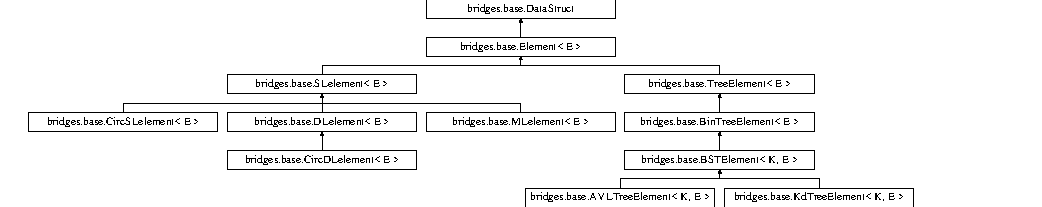
\includegraphics[height=4.647303cm]{classbridges_1_1base_1_1_element}
\end{center}
\end{figure}
\subsection*{Public Member Functions}
\begin{DoxyCompactItemize}
\item 
\hyperlink{classbridges_1_1base_1_1_element_aa5fc5728f2ed4b041118a77409442390}{Element} ()
\item 
\hyperlink{classbridges_1_1base_1_1_element_a6cb9b3b85b923602aad5c1be6696d825}{Element} (E val)
\item 
\hyperlink{classbridges_1_1base_1_1_element_a14e857e8050eac518900a458f0364d8e}{Element} (String label, E val)
\item 
\hyperlink{classbridges_1_1base_1_1_element_a91db9de70b65a1d7b5f27c1c0b909832}{Element} (\hyperlink{classbridges_1_1base_1_1_element}{Element}$<$ E $>$ original)
\item 
String \hyperlink{classbridges_1_1base_1_1_element_ad5496f568b4cca3909800eceea5fb47d}{get\+Identifier} ()
\item 
\hyperlink{classbridges_1_1base_1_1_element_visualizer}{Element\+Visualizer} \hyperlink{classbridges_1_1base_1_1_element_a42c84d41dfb7bd05a586e303cb33de72}{get\+Visualizer} ()
\item 
void \hyperlink{classbridges_1_1base_1_1_element_a5befa95788099f1bc72cdf5361c55bed}{set\+Visualizer} (\hyperlink{classbridges_1_1base_1_1_element_visualizer}{Element\+Visualizer} visualizer)
\item 
\hyperlink{classbridges_1_1base_1_1_link_visualizer}{Link\+Visualizer} \hyperlink{classbridges_1_1base_1_1_element_a7978552c7b36e28c302f611fc1958e7f}{get\+Link\+Visualizer} (\hyperlink{classbridges_1_1base_1_1_element}{Element}$<$ E $>$ el)
\item 
String \hyperlink{classbridges_1_1base_1_1_element_aa235244426486921bef319a28616bf8b}{get\+Class\+Name} ()
\item 
int \hyperlink{classbridges_1_1base_1_1_element_a6cd4c4f15c6a4f87f59e443cffe87a20}{compare\+To} (\hyperlink{classbridges_1_1base_1_1_element}{Element}$<$ E $>$ e1)
\item 
boolean \hyperlink{classbridges_1_1base_1_1_element_aff10d60700eb1aceca5c0b519bdccccb}{equals} (\hyperlink{classbridges_1_1base_1_1_element}{Element}$<$ E $>$ e1)
\item 
String \hyperlink{classbridges_1_1base_1_1_element_a16c4c7e0d511fbf0e205d5606b9d690e}{get\+Representation} ()
\item 
String \hyperlink{classbridges_1_1base_1_1_element_a5c831a0238de487765f6021a887f1542}{get\+Label} ()
\item 
void \hyperlink{classbridges_1_1base_1_1_element_a942ccd766aeca0c4fdbe27ef8cbe78d9}{set\+Label} (String label)
\item 
String \hyperlink{classbridges_1_1base_1_1_element_acd2191242df8a7bf2e8b6ced87880ba6}{arrange\+Label} (String label, int word\+Number)
\item 
E \hyperlink{classbridges_1_1base_1_1_element_a44ddc61db34b6cf0bab7dfba667d54af}{get\+Value} ()
\item 
void \hyperlink{classbridges_1_1base_1_1_element_ab3cf1241da0bc4c59cea9d6f0fd7aaf4}{set\+Value} (E value)
\item 
String \hyperlink{classbridges_1_1base_1_1_element_a7dc685e317fd9dc2e73e049a9f907e42}{to\+String} ()
\end{DoxyCompactItemize}
\subsection*{Protected Member Functions}
\begin{DoxyCompactItemize}
\item 
String \hyperlink{classbridges_1_1base_1_1_element_a6a1b70fa4b1936d10c6deb433acf8cd9}{get\+Data\+Struct\+Type} ()
\item 
void \hyperlink{classbridges_1_1base_1_1_element_af1a60f4e6a91d379179f7d56e6dc3829}{validate\+Val} (E value)
\end{DoxyCompactItemize}
\subsection*{Additional Inherited Members}


\subsection{Detailed Description}
This is the main superclass in B\+R\+I\+D\+G\+ES for deriving a number of objects used in building arrays, lists, trees and graph data structures. 

\hyperlink{classbridges_1_1base_1_1_d_lelement}{D\+Lelement}, \hyperlink{classbridges_1_1base_1_1_circ_s_lelement}{Circ\+S\+Lelement}, \hyperlink{classbridges_1_1base_1_1_circ_d_lelement}{Circ\+D\+Lelement}, \hyperlink{classbridges_1_1base_1_1_tree_element}{Tree\+Element}, \hyperlink{classbridges_1_1base_1_1_bin_tree_element}{Bin\+Tree\+Element}, \hyperlink{classbridges_1_1base_1_1_b_s_t_element}{B\+S\+T\+Element}, \hyperlink{classbridges_1_1base_1_1_a_v_l_tree_element}{A\+V\+L\+Tree\+Element} are all subclasses. \hyperlink{classbridges_1_1base_1_1_element}{Element} contains visualizer objects (\hyperlink{classbridges_1_1base_1_1_element_visualizer}{Element\+Visualizer}, \hyperlink{classbridges_1_1base_1_1_link_visualizer}{Link\+Visualizer}) for specifying visual attributes. It also contains a label that is used in the visualization.

\begin{DoxyAuthor}{Author}
Mihai Mehedint, Kalpathi Subramanian
\end{DoxyAuthor}

\begin{DoxyParams}{Parameters}
{\em generic} & $<$\+E$>$ \\
\hline
\end{DoxyParams}


\subsection{Constructor \& Destructor Documentation}
\hypertarget{classbridges_1_1base_1_1_element_aa5fc5728f2ed4b041118a77409442390}{}\label{classbridges_1_1base_1_1_element_aa5fc5728f2ed4b041118a77409442390} 
\index{bridges\+::base\+::\+Element@{bridges\+::base\+::\+Element}!Element@{Element}}
\index{Element@{Element}!bridges\+::base\+::\+Element@{bridges\+::base\+::\+Element}}
\subsubsection{\texorpdfstring{Element()}{Element()}\hspace{0.1cm}{\footnotesize\ttfamily [1/4]}}
{\footnotesize\ttfamily \hyperlink{classbridges_1_1base_1_1_element}{bridges.\+base.\+Element}$<$ E $>$.\hyperlink{classbridges_1_1base_1_1_element}{Element} (\begin{DoxyParamCaption}{ }\end{DoxyParamCaption})}

\hyperlink{classbridges_1_1base_1_1_element}{Element} constructor creates an \hyperlink{classbridges_1_1base_1_1_element_visualizer}{Element\+Visualizer} object sets a unique identifier for the current \hyperlink{classbridges_1_1base_1_1_element}{Element} normally used from subclasses \hypertarget{classbridges_1_1base_1_1_element_a6cb9b3b85b923602aad5c1be6696d825}{}\label{classbridges_1_1base_1_1_element_a6cb9b3b85b923602aad5c1be6696d825} 
\index{bridges\+::base\+::\+Element@{bridges\+::base\+::\+Element}!Element@{Element}}
\index{Element@{Element}!bridges\+::base\+::\+Element@{bridges\+::base\+::\+Element}}
\subsubsection{\texorpdfstring{Element()}{Element()}\hspace{0.1cm}{\footnotesize\ttfamily [2/4]}}
{\footnotesize\ttfamily \hyperlink{classbridges_1_1base_1_1_element}{bridges.\+base.\+Element}$<$ E $>$.\hyperlink{classbridges_1_1base_1_1_element}{Element} (\begin{DoxyParamCaption}\item[{E}]{val }\end{DoxyParamCaption})}

the constructor of \hyperlink{classbridges_1_1base_1_1_element}{Element} 
\begin{DoxyParams}{Parameters}
{\em val} & will be used to construct \hyperlink{classbridges_1_1base_1_1_element}{Element} \\
\hline
\end{DoxyParams}
\hypertarget{classbridges_1_1base_1_1_element_a14e857e8050eac518900a458f0364d8e}{}\label{classbridges_1_1base_1_1_element_a14e857e8050eac518900a458f0364d8e} 
\index{bridges\+::base\+::\+Element@{bridges\+::base\+::\+Element}!Element@{Element}}
\index{Element@{Element}!bridges\+::base\+::\+Element@{bridges\+::base\+::\+Element}}
\subsubsection{\texorpdfstring{Element()}{Element()}\hspace{0.1cm}{\footnotesize\ttfamily [3/4]}}
{\footnotesize\ttfamily \hyperlink{classbridges_1_1base_1_1_element}{bridges.\+base.\+Element}$<$ E $>$.\hyperlink{classbridges_1_1base_1_1_element}{Element} (\begin{DoxyParamCaption}\item[{String}]{label,  }\item[{E}]{val }\end{DoxyParamCaption})}

the constructor of \hyperlink{classbridges_1_1base_1_1_element}{Element} 
\begin{DoxyParams}{Parameters}
{\em label} & the string that is visible on the Bridges Visualization \\
\hline
{\em val} & will be used to construct \hyperlink{classbridges_1_1base_1_1_element}{Element} \\
\hline
\end{DoxyParams}
\hypertarget{classbridges_1_1base_1_1_element_a91db9de70b65a1d7b5f27c1c0b909832}{}\label{classbridges_1_1base_1_1_element_a91db9de70b65a1d7b5f27c1c0b909832} 
\index{bridges\+::base\+::\+Element@{bridges\+::base\+::\+Element}!Element@{Element}}
\index{Element@{Element}!bridges\+::base\+::\+Element@{bridges\+::base\+::\+Element}}
\subsubsection{\texorpdfstring{Element()}{Element()}\hspace{0.1cm}{\footnotesize\ttfamily [4/4]}}
{\footnotesize\ttfamily \hyperlink{classbridges_1_1base_1_1_element}{bridges.\+base.\+Element}$<$ E $>$.\hyperlink{classbridges_1_1base_1_1_element}{Element} (\begin{DoxyParamCaption}\item[{\hyperlink{classbridges_1_1base_1_1_element}{Element}$<$ E $>$}]{original }\end{DoxyParamCaption})}

performing deep copy of an element when needed 
\begin{DoxyParams}{Parameters}
{\em original} & the \hyperlink{classbridges_1_1base_1_1_element}{Element} that is to be copied \\
\hline
\end{DoxyParams}


\subsection{Member Function Documentation}
\hypertarget{classbridges_1_1base_1_1_element_acd2191242df8a7bf2e8b6ced87880ba6}{}\label{classbridges_1_1base_1_1_element_acd2191242df8a7bf2e8b6ced87880ba6} 
\index{bridges\+::base\+::\+Element@{bridges\+::base\+::\+Element}!arrange\+Label@{arrange\+Label}}
\index{arrange\+Label@{arrange\+Label}!bridges\+::base\+::\+Element@{bridges\+::base\+::\+Element}}
\subsubsection{\texorpdfstring{arrange\+Label()}{arrangeLabel()}}
{\footnotesize\ttfamily String \hyperlink{classbridges_1_1base_1_1_element}{bridges.\+base.\+Element}$<$ E $>$.arrange\+Label (\begin{DoxyParamCaption}\item[{String}]{label,  }\item[{int}]{word\+Number }\end{DoxyParamCaption})}

This method formats the label string using a predefine pattern (D\+I\+V\+I\+D\+E\+\_\+\+K\+EY) and replaces the pattern with the string characters hold by the I\+N\+S\+E\+R\+T\+\_\+\+S\+T\+R\+I\+NG global variable 
\begin{DoxyParams}{Parameters}
{\em label} & \\
\hline
{\em word\+Number} & in very long strings in the case where the whitespace \textbackslash{}s is chosen as a key the word\+Number can be set to replace the whitespace with a newline character \textbackslash{}n at a given number of words (every second or third word) The default value is 0. In most situations we want to replace all patterns found. for more complex patterns the key must be changed like so \char`\"{}((\+John) (.+?))\char`\"{} returns \char`\"{}\+John first\+Word\+After\+John\char`\"{}\+: John writes, John doe, John eats etc. (\textbackslash{}w) matches any word (\textbackslash{}s) one white space (\textbackslash{}s$\ast$) zero or more white spaces, (\textbackslash{}s+) one or more\\
\hline
\end{DoxyParams}
\begin{DoxyReturn}{Returns}

\end{DoxyReturn}
\hypertarget{classbridges_1_1base_1_1_element_a6cd4c4f15c6a4f87f59e443cffe87a20}{}\label{classbridges_1_1base_1_1_element_a6cd4c4f15c6a4f87f59e443cffe87a20} 
\index{bridges\+::base\+::\+Element@{bridges\+::base\+::\+Element}!compare\+To@{compare\+To}}
\index{compare\+To@{compare\+To}!bridges\+::base\+::\+Element@{bridges\+::base\+::\+Element}}
\subsubsection{\texorpdfstring{compare\+To()}{compareTo()}}
{\footnotesize\ttfamily int \hyperlink{classbridges_1_1base_1_1_element}{bridges.\+base.\+Element}$<$ E $>$.compare\+To (\begin{DoxyParamCaption}\item[{\hyperlink{classbridges_1_1base_1_1_element}{Element}$<$ E $>$}]{e1 }\end{DoxyParamCaption})}

Comparison between 2 elements 
\begin{DoxyParams}{Parameters}
{\em e1} & the \hyperlink{classbridges_1_1base_1_1_element}{Element} to compare this with \\
\hline
\end{DoxyParams}
\begin{DoxyReturn}{Returns}
0 if the 2 elements have the same label and the same identifier and a non\+Zero integer otherwise 
\end{DoxyReturn}
\hypertarget{classbridges_1_1base_1_1_element_aff10d60700eb1aceca5c0b519bdccccb}{}\label{classbridges_1_1base_1_1_element_aff10d60700eb1aceca5c0b519bdccccb} 
\index{bridges\+::base\+::\+Element@{bridges\+::base\+::\+Element}!equals@{equals}}
\index{equals@{equals}!bridges\+::base\+::\+Element@{bridges\+::base\+::\+Element}}
\subsubsection{\texorpdfstring{equals()}{equals()}}
{\footnotesize\ttfamily boolean \hyperlink{classbridges_1_1base_1_1_element}{bridges.\+base.\+Element}$<$ E $>$.equals (\begin{DoxyParamCaption}\item[{\hyperlink{classbridges_1_1base_1_1_element}{Element}$<$ E $>$}]{e1 }\end{DoxyParamCaption})}

This method compares 2 Elements 
\begin{DoxyParams}{Parameters}
{\em e1} & \\
\hline
\end{DoxyParams}
\begin{DoxyReturn}{Returns}
boolean 
\end{DoxyReturn}
\hypertarget{classbridges_1_1base_1_1_element_aa235244426486921bef319a28616bf8b}{}\label{classbridges_1_1base_1_1_element_aa235244426486921bef319a28616bf8b} 
\index{bridges\+::base\+::\+Element@{bridges\+::base\+::\+Element}!get\+Class\+Name@{get\+Class\+Name}}
\index{get\+Class\+Name@{get\+Class\+Name}!bridges\+::base\+::\+Element@{bridges\+::base\+::\+Element}}
\subsubsection{\texorpdfstring{get\+Class\+Name()}{getClassName()}}
{\footnotesize\ttfamily String \hyperlink{classbridges_1_1base_1_1_element}{bridges.\+base.\+Element}$<$ E $>$.get\+Class\+Name (\begin{DoxyParamCaption}{ }\end{DoxyParamCaption})}

This method returns the name of the class \begin{DoxyReturn}{Returns}
the class name \char`\"{}\+Element\char`\"{} 
\end{DoxyReturn}
\hypertarget{classbridges_1_1base_1_1_element_a6a1b70fa4b1936d10c6deb433acf8cd9}{}\label{classbridges_1_1base_1_1_element_a6a1b70fa4b1936d10c6deb433acf8cd9} 
\index{bridges\+::base\+::\+Element@{bridges\+::base\+::\+Element}!get\+Data\+Struct\+Type@{get\+Data\+Struct\+Type}}
\index{get\+Data\+Struct\+Type@{get\+Data\+Struct\+Type}!bridges\+::base\+::\+Element@{bridges\+::base\+::\+Element}}
\subsubsection{\texorpdfstring{get\+Data\+Struct\+Type()}{getDataStructType()}}
{\footnotesize\ttfamily String \hyperlink{classbridges_1_1base_1_1_element}{bridges.\+base.\+Element}$<$ E $>$.get\+Data\+Struct\+Type (\begin{DoxyParamCaption}{ }\end{DoxyParamCaption})\hspace{0.3cm}{\ttfamily [protected]}}

\hypertarget{classbridges_1_1base_1_1_element_ad5496f568b4cca3909800eceea5fb47d}{}\label{classbridges_1_1base_1_1_element_ad5496f568b4cca3909800eceea5fb47d} 
\index{bridges\+::base\+::\+Element@{bridges\+::base\+::\+Element}!get\+Identifier@{get\+Identifier}}
\index{get\+Identifier@{get\+Identifier}!bridges\+::base\+::\+Element@{bridges\+::base\+::\+Element}}
\subsubsection{\texorpdfstring{get\+Identifier()}{getIdentifier()}}
{\footnotesize\ttfamily String \hyperlink{classbridges_1_1base_1_1_element}{bridges.\+base.\+Element}$<$ E $>$.get\+Identifier (\begin{DoxyParamCaption}{ }\end{DoxyParamCaption})}

this method returns the element\textquotesingle{}s unique identifier \begin{DoxyReturn}{Returns}
the string identifier 
\end{DoxyReturn}
\hypertarget{classbridges_1_1base_1_1_element_a5c831a0238de487765f6021a887f1542}{}\label{classbridges_1_1base_1_1_element_a5c831a0238de487765f6021a887f1542} 
\index{bridges\+::base\+::\+Element@{bridges\+::base\+::\+Element}!get\+Label@{get\+Label}}
\index{get\+Label@{get\+Label}!bridges\+::base\+::\+Element@{bridges\+::base\+::\+Element}}
\subsubsection{\texorpdfstring{get\+Label()}{getLabel()}}
{\footnotesize\ttfamily String \hyperlink{classbridges_1_1base_1_1_element}{bridges.\+base.\+Element}$<$ E $>$.get\+Label (\begin{DoxyParamCaption}{ }\end{DoxyParamCaption})}

This method returns the existing value of the label fields \begin{DoxyReturn}{Returns}
the label of the \hyperlink{classbridges_1_1base_1_1_element}{Element} that shows up on the Bridges Visualization 
\end{DoxyReturn}
\hypertarget{classbridges_1_1base_1_1_element_a7978552c7b36e28c302f611fc1958e7f}{}\label{classbridges_1_1base_1_1_element_a7978552c7b36e28c302f611fc1958e7f} 
\index{bridges\+::base\+::\+Element@{bridges\+::base\+::\+Element}!get\+Link\+Visualizer@{get\+Link\+Visualizer}}
\index{get\+Link\+Visualizer@{get\+Link\+Visualizer}!bridges\+::base\+::\+Element@{bridges\+::base\+::\+Element}}
\subsubsection{\texorpdfstring{get\+Link\+Visualizer()}{getLinkVisualizer()}}
{\footnotesize\ttfamily \hyperlink{classbridges_1_1base_1_1_link_visualizer}{Link\+Visualizer} \hyperlink{classbridges_1_1base_1_1_element}{bridges.\+base.\+Element}$<$ E $>$.get\+Link\+Visualizer (\begin{DoxyParamCaption}\item[{\hyperlink{classbridges_1_1base_1_1_element}{Element}$<$ E $>$}]{el }\end{DoxyParamCaption})}

Returns the \hyperlink{classbridges_1_1base_1_1_element}{Element}\textquotesingle{}s link visualizer object that is linked to element el  \hyperlink{classbridges_1_1base_1_1_element}{Element} el -- the element terminating the link \begin{DoxyReturn}{Returns}
the link visualizer 
\end{DoxyReturn}
\hypertarget{classbridges_1_1base_1_1_element_a16c4c7e0d511fbf0e205d5606b9d690e}{}\label{classbridges_1_1base_1_1_element_a16c4c7e0d511fbf0e205d5606b9d690e} 
\index{bridges\+::base\+::\+Element@{bridges\+::base\+::\+Element}!get\+Representation@{get\+Representation}}
\index{get\+Representation@{get\+Representation}!bridges\+::base\+::\+Element@{bridges\+::base\+::\+Element}}
\subsubsection{\texorpdfstring{get\+Representation()}{getRepresentation()}}
{\footnotesize\ttfamily String \hyperlink{classbridges_1_1base_1_1_element}{bridges.\+base.\+Element}$<$ E $>$.get\+Representation (\begin{DoxyParamCaption}{ }\end{DoxyParamCaption})}

Internal code for getting the properties of the \hyperlink{classbridges_1_1base_1_1_element}{Element} object. It produces (without the spaces or newlines)\+: \{ \char`\"{}name\char`\"{}\+: \char`\"{}\+Some label\char`\"{}, \char`\"{}other C\+S\+S properties like color\char`\"{}\+: any\+\_\+\+J\+S\+O\+N\+\_\+value \} \begin{DoxyReturn}{Returns}
the encoded J\+S\+ON string 
\end{DoxyReturn}
\hypertarget{classbridges_1_1base_1_1_element_a44ddc61db34b6cf0bab7dfba667d54af}{}\label{classbridges_1_1base_1_1_element_a44ddc61db34b6cf0bab7dfba667d54af} 
\index{bridges\+::base\+::\+Element@{bridges\+::base\+::\+Element}!get\+Value@{get\+Value}}
\index{get\+Value@{get\+Value}!bridges\+::base\+::\+Element@{bridges\+::base\+::\+Element}}
\subsubsection{\texorpdfstring{get\+Value()}{getValue()}}
{\footnotesize\ttfamily E \hyperlink{classbridges_1_1base_1_1_element}{bridges.\+base.\+Element}$<$ E $>$.get\+Value (\begin{DoxyParamCaption}{ }\end{DoxyParamCaption})}

this method returns the value E for the current \hyperlink{classbridges_1_1base_1_1_element}{Element} \begin{DoxyReturn}{Returns}
the value 
\end{DoxyReturn}
\hypertarget{classbridges_1_1base_1_1_element_a42c84d41dfb7bd05a586e303cb33de72}{}\label{classbridges_1_1base_1_1_element_a42c84d41dfb7bd05a586e303cb33de72} 
\index{bridges\+::base\+::\+Element@{bridges\+::base\+::\+Element}!get\+Visualizer@{get\+Visualizer}}
\index{get\+Visualizer@{get\+Visualizer}!bridges\+::base\+::\+Element@{bridges\+::base\+::\+Element}}
\subsubsection{\texorpdfstring{get\+Visualizer()}{getVisualizer()}}
{\footnotesize\ttfamily \hyperlink{classbridges_1_1base_1_1_element_visualizer}{Element\+Visualizer} \hyperlink{classbridges_1_1base_1_1_element}{bridges.\+base.\+Element}$<$ E $>$.get\+Visualizer (\begin{DoxyParamCaption}{ }\end{DoxyParamCaption})}

Returns the \hyperlink{classbridges_1_1base_1_1_element}{Element}\textquotesingle{}s visualizer object \begin{DoxyReturn}{Returns}
the visualizer 
\end{DoxyReturn}
\hypertarget{classbridges_1_1base_1_1_element_a942ccd766aeca0c4fdbe27ef8cbe78d9}{}\label{classbridges_1_1base_1_1_element_a942ccd766aeca0c4fdbe27ef8cbe78d9} 
\index{bridges\+::base\+::\+Element@{bridges\+::base\+::\+Element}!set\+Label@{set\+Label}}
\index{set\+Label@{set\+Label}!bridges\+::base\+::\+Element@{bridges\+::base\+::\+Element}}
\subsubsection{\texorpdfstring{set\+Label()}{setLabel()}}
{\footnotesize\ttfamily void \hyperlink{classbridges_1_1base_1_1_element}{bridges.\+base.\+Element}$<$ E $>$.set\+Label (\begin{DoxyParamCaption}\item[{String}]{label }\end{DoxyParamCaption})}

This method sets the label 
\begin{DoxyParams}{Parameters}
{\em label} & the label to set \\
\hline
\end{DoxyParams}
\hypertarget{classbridges_1_1base_1_1_element_ab3cf1241da0bc4c59cea9d6f0fd7aaf4}{}\label{classbridges_1_1base_1_1_element_ab3cf1241da0bc4c59cea9d6f0fd7aaf4} 
\index{bridges\+::base\+::\+Element@{bridges\+::base\+::\+Element}!set\+Value@{set\+Value}}
\index{set\+Value@{set\+Value}!bridges\+::base\+::\+Element@{bridges\+::base\+::\+Element}}
\subsubsection{\texorpdfstring{set\+Value()}{setValue()}}
{\footnotesize\ttfamily void \hyperlink{classbridges_1_1base_1_1_element}{bridges.\+base.\+Element}$<$ E $>$.set\+Value (\begin{DoxyParamCaption}\item[{E}]{value }\end{DoxyParamCaption})}

This method sets the value field to the E argument value 
\begin{DoxyParams}{Parameters}
{\em value} & the value to set \\
\hline
\end{DoxyParams}
\hypertarget{classbridges_1_1base_1_1_element_a5befa95788099f1bc72cdf5361c55bed}{}\label{classbridges_1_1base_1_1_element_a5befa95788099f1bc72cdf5361c55bed} 
\index{bridges\+::base\+::\+Element@{bridges\+::base\+::\+Element}!set\+Visualizer@{set\+Visualizer}}
\index{set\+Visualizer@{set\+Visualizer}!bridges\+::base\+::\+Element@{bridges\+::base\+::\+Element}}
\subsubsection{\texorpdfstring{set\+Visualizer()}{setVisualizer()}}
{\footnotesize\ttfamily void \hyperlink{classbridges_1_1base_1_1_element}{bridges.\+base.\+Element}$<$ E $>$.set\+Visualizer (\begin{DoxyParamCaption}\item[{\hyperlink{classbridges_1_1base_1_1_element_visualizer}{Element\+Visualizer}}]{visualizer }\end{DoxyParamCaption})}

This method sets the visualizer object for the current element object 
\begin{DoxyParams}{Parameters}
{\em visualizer} & the visualizer to set \\
\hline
\end{DoxyParams}
\hypertarget{classbridges_1_1base_1_1_element_a7dc685e317fd9dc2e73e049a9f907e42}{}\label{classbridges_1_1base_1_1_element_a7dc685e317fd9dc2e73e049a9f907e42} 
\index{bridges\+::base\+::\+Element@{bridges\+::base\+::\+Element}!to\+String@{to\+String}}
\index{to\+String@{to\+String}!bridges\+::base\+::\+Element@{bridges\+::base\+::\+Element}}
\subsubsection{\texorpdfstring{to\+String()}{toString()}}
{\footnotesize\ttfamily String \hyperlink{classbridges_1_1base_1_1_element}{bridges.\+base.\+Element}$<$ E $>$.to\+String (\begin{DoxyParamCaption}{ }\end{DoxyParamCaption})}

\hypertarget{classbridges_1_1base_1_1_element_af1a60f4e6a91d379179f7d56e6dc3829}{}\label{classbridges_1_1base_1_1_element_af1a60f4e6a91d379179f7d56e6dc3829} 
\index{bridges\+::base\+::\+Element@{bridges\+::base\+::\+Element}!validate\+Val@{validate\+Val}}
\index{validate\+Val@{validate\+Val}!bridges\+::base\+::\+Element@{bridges\+::base\+::\+Element}}
\subsubsection{\texorpdfstring{validate\+Val()}{validateVal()}}
{\footnotesize\ttfamily void \hyperlink{classbridges_1_1base_1_1_element}{bridges.\+base.\+Element}$<$ E $>$.validate\+Val (\begin{DoxyParamCaption}\item[{E}]{value }\end{DoxyParamCaption})\hspace{0.3cm}{\ttfamily [protected]}}

Validates the \hyperlink{classbridges_1_1base_1_1_element}{Element}\textquotesingle{}s value when the \hyperlink{classbridges_1_1base_1_1_element}{Element} is created A non null value is expected this will be unnecessary after we modify the server 
\begin{DoxyParams}{Parameters}
{\em E\+Lement} & value \\
\hline
\end{DoxyParams}


The documentation for this class was generated from the following file\+:\begin{DoxyCompactItemize}
\item 
/\+Users/kalpathi/gr/bridges/client/java/bridges16/src/main/java/edu/uncc/cs/bridges\+\_\+v21/base/\hyperlink{_element_8java}{Element.\+java}\end{DoxyCompactItemize}

\hypertarget{classbridges_1_1base_1_1_element_visualizer}{}\section{bridges.\+base.\+Element\+Visualizer Class Reference}
\label{classbridges_1_1base_1_1_element_visualizer}\index{bridges.\+base.\+Element\+Visualizer@{bridges.\+base.\+Element\+Visualizer}}


This class maintains the visual attributes of each B\+R\+I\+D\+G\+E\+S element.  


\subsection*{Public Member Functions}
\begin{DoxyCompactItemize}
\item 
\hyperlink{classbridges_1_1base_1_1_element_visualizer_acbca874876ec1e8dbbde6484a4fc056e}{Element\+Visualizer} ()
\item 
\hyperlink{classbridges_1_1base_1_1_element_visualizer_a5c0d9fe8051ebc816372b9836689fdfa}{Element\+Visualizer} (String a\+Color)
\item 
\hyperlink{classbridges_1_1base_1_1_element_visualizer_ab62b1b06907fbeddfcee2b4b297e1021}{Element\+Visualizer} (String a\+Color, String a\+Shape)
\item 
\hyperlink{classbridges_1_1base_1_1_element_visualizer_ab32f66b72ccf0a26c03ba44006da9ac6}{Element\+Visualizer} (double size)
\item 
\hyperlink{classbridges_1_1base_1_1_element_visualizer_a9bf06ca1b6c215e079ab33ccd99633e8}{Element\+Visualizer} (String a\+Color, String a\+Shape, float opacity, double size)
\item 
\hyperlink{classbridges_1_1base_1_1_element_visualizer_a5b48cbda94a4e84e40de41fe156e2497}{Element\+Visualizer} (\hyperlink{classbridges_1_1base_1_1_element_visualizer}{Element\+Visualizer} v)
\item 
void \hyperlink{classbridges_1_1base_1_1_element_visualizer_aba410184f7df495594fc1fa7948335a5}{set\+Size} (double sz)
\item 
double \hyperlink{classbridges_1_1base_1_1_element_visualizer_a0b7673bf724e3df1f94df50ad95ca5b1}{get\+Size} ()
\item 
void \hyperlink{classbridges_1_1base_1_1_element_visualizer_ad7ff2a772741301c08943a58ffccca38}{set\+Color} (String col\+\_\+name)  throws Invalid\+Value\+Exception 
\item 
void \hyperlink{classbridges_1_1base_1_1_element_visualizer_a84fad1c8abe43b20c68c1800d7630918}{set\+Color} (Integer r, Integer g, Integer b, float a)
\item 
void \hyperlink{classbridges_1_1base_1_1_element_visualizer_a33172ab908f3b6f9740727b0bfe91565}{set\+Color} (\hyperlink{classbridges_1_1base_1_1_color}{Color} c)
\item 
\hyperlink{classbridges_1_1base_1_1_color}{Color} \hyperlink{classbridges_1_1base_1_1_element_visualizer_a3bf821b9bfa02746882bac934ce4fb8e}{get\+Color} ()
\item 
String \hyperlink{classbridges_1_1base_1_1_element_visualizer_a8ef0825745e49f32b57e4bf6c891b57e}{get\+Shape} ()
\item 
void \hyperlink{classbridges_1_1base_1_1_element_visualizer_ac3bad991904c8ad23e5233b341381d93}{set\+Shape} (String a\+Shape)
\item 
void \hyperlink{classbridges_1_1base_1_1_element_visualizer_a932f62eb1bd0c92da265a7f903dd0790}{set\+Opacity} (float opacity)
\item 
float \hyperlink{classbridges_1_1base_1_1_element_visualizer_ab86ff39f17f8d1766670b18be88b5492}{get\+Opacity} ()
\item 
void \hyperlink{classbridges_1_1base_1_1_element_visualizer_a04f3416447f2042de7cd21ce5b6a0598}{set\+Location} (double x, double y)
\end{DoxyCompactItemize}


\subsection{Detailed Description}
This class maintains the visual attributes of each B\+R\+I\+D\+G\+E\+S element. 

Visual properties include color, shape, opacity, size and location. Objects of this class are stored as part of the \hyperlink{classbridges_1_1base_1_1_element}{Element} class. Generally, a user will manipulate the \hyperlink{classbridges_1_1base_1_1_element_visualizer}{Element\+Visualizer} returned from the \hyperlink{classbridges_1_1base_1_1_element}{Element}\textquotesingle{}s get\+Visualizer() method, and then set attributes using its methods. Supported attributed values are as follows\+:~\newline


{\bfseries Supported Colors (by name)}\+: 

\char`\"{}red\char`\"{}, \char`\"{}green\char`\"{}, \char`\"{}blue\char`\"{},\char`\"{}yellow\char`\"{},\char`\"{}cyan\char`\"{},\char`\"{}magenta\char`\"{}, \char`\"{}white\char`\"{},, \char`\"{}black\char`\"{}, \char`\"{}orange\char`\"{}, \char`\"{}turquoise\char`\"{}, \char`\"{}maroon\char`\"{}, ~\newline
 \char`\"{}aquamarine\char`\"{}, \char`\"{}azure\char`\"{}, \char`\"{}beige\char`\"{}, \char`\"{}brown\char`\"{}, \char`\"{}tan\char`\"{}, \char`\"{}olive\char`\"{}, \char`\"{}chartreuse\char`\"{}, \char`\"{}khaki\char`\"{}, \char`\"{}bisque\char`\"{}, \char`\"{}coral\char`\"{}, ~\newline
 \char`\"{}pink\char`\"{}, \char`\"{}lavender\char`\"{}, \char`\"{}purple\char`\"{}, \char`\"{}gold\char`\"{} 

{\bfseries  \hyperlink{classbridges_1_1base_1_1_color}{Color} by R\+G\+B\+A Specification \+:} Range\+: 0-\/255 for each component 

{\bfseries Supported Shapes\+: }

\char`\"{}circle\char`\"{}, \char`\"{}square\char`\"{}, \char`\"{}diamond\char`\"{}, \char`\"{}cross\char`\"{}, \char`\"{}triangle\char`\"{}, \char`\"{}star\char`\"{}, \char`\"{}wye\char`\"{} 

{\bfseries  Shape Size} \+: Range (0-\/50) 

{\bfseries  Opacity\+: } Range (0.\+0-\/1.\+0) 

\begin{DoxyAuthor}{Author}
Mihai Mehedint, Kalpathi Subramanian
\end{DoxyAuthor}
\begin{DoxyDate}{Date}
6/22/16, 1/7/17, 5/17/17
\end{DoxyDate}
\begin{DoxySeeAlso}{See also}
Example Tutorial at ~\newline
 \href{http://bridgesuncc.github.io/Hello_World_Tutorials/SLL.html}{\tt http\+://bridgesuncc.\+github.\+io/\+Hello\+\_\+\+World\+\_\+\+Tutorials/\+S\+L\+L.\+html} 
\end{DoxySeeAlso}


\subsection{Constructor \& Destructor Documentation}
\hypertarget{classbridges_1_1base_1_1_element_visualizer_acbca874876ec1e8dbbde6484a4fc056e}{}\index{bridges\+::base\+::\+Element\+Visualizer@{bridges\+::base\+::\+Element\+Visualizer}!Element\+Visualizer@{Element\+Visualizer}}
\index{Element\+Visualizer@{Element\+Visualizer}!bridges\+::base\+::\+Element\+Visualizer@{bridges\+::base\+::\+Element\+Visualizer}}
\subsubsection[{Element\+Visualizer()}]{\setlength{\rightskip}{0pt plus 5cm}bridges.\+base.\+Element\+Visualizer.\+Element\+Visualizer (
\begin{DoxyParamCaption}
{}
\end{DoxyParamCaption}
)}\label{classbridges_1_1base_1_1_element_visualizer_acbca874876ec1e8dbbde6484a4fc056e}
Construct an \hyperlink{classbridges_1_1base_1_1_element_visualizer}{Element\+Visualizer} with the default visualization settings.

The default settings are color = green, opacity = 1.\+0, size = 10.\+0, shape = circle. \hypertarget{classbridges_1_1base_1_1_element_visualizer_a5c0d9fe8051ebc816372b9836689fdfa}{}\index{bridges\+::base\+::\+Element\+Visualizer@{bridges\+::base\+::\+Element\+Visualizer}!Element\+Visualizer@{Element\+Visualizer}}
\index{Element\+Visualizer@{Element\+Visualizer}!bridges\+::base\+::\+Element\+Visualizer@{bridges\+::base\+::\+Element\+Visualizer}}
\subsubsection[{Element\+Visualizer(\+String a\+Color)}]{\setlength{\rightskip}{0pt plus 5cm}bridges.\+base.\+Element\+Visualizer.\+Element\+Visualizer (
\begin{DoxyParamCaption}
\item[{String}]{a\+Color}
\end{DoxyParamCaption}
)}\label{classbridges_1_1base_1_1_element_visualizer_a5c0d9fe8051ebc816372b9836689fdfa}
Construct an \hyperlink{classbridges_1_1base_1_1_element_visualizer}{Element\+Visualizer} with its color set to \char`\"{}a\+Color\char`\"{}.


\begin{DoxyParams}{Parameters}
{\em a\+Color} & the string that represents one of the Bridges colors. \\
\hline
\end{DoxyParams}
\hypertarget{classbridges_1_1base_1_1_element_visualizer_ab62b1b06907fbeddfcee2b4b297e1021}{}\index{bridges\+::base\+::\+Element\+Visualizer@{bridges\+::base\+::\+Element\+Visualizer}!Element\+Visualizer@{Element\+Visualizer}}
\index{Element\+Visualizer@{Element\+Visualizer}!bridges\+::base\+::\+Element\+Visualizer@{bridges\+::base\+::\+Element\+Visualizer}}
\subsubsection[{Element\+Visualizer(\+String a\+Color, String a\+Shape)}]{\setlength{\rightskip}{0pt plus 5cm}bridges.\+base.\+Element\+Visualizer.\+Element\+Visualizer (
\begin{DoxyParamCaption}
\item[{String}]{a\+Color, }
\item[{String}]{a\+Shape}
\end{DoxyParamCaption}
)}\label{classbridges_1_1base_1_1_element_visualizer_ab62b1b06907fbeddfcee2b4b297e1021}
Construct an \hyperlink{classbridges_1_1base_1_1_element_visualizer}{Element\+Visualizer} with its color set to \char`\"{}a\+Color\char`\"{} and shape set to \char`\"{}a\+Shape\char`\"{}.


\begin{DoxyParams}{Parameters}
{\em a\+Color} & the string that represents one of the Bridges colors. \\
\hline
{\em a\+Shape} & the string that represents one of the Bridges shapes \\
\hline
\end{DoxyParams}
\hypertarget{classbridges_1_1base_1_1_element_visualizer_ab32f66b72ccf0a26c03ba44006da9ac6}{}\index{bridges\+::base\+::\+Element\+Visualizer@{bridges\+::base\+::\+Element\+Visualizer}!Element\+Visualizer@{Element\+Visualizer}}
\index{Element\+Visualizer@{Element\+Visualizer}!bridges\+::base\+::\+Element\+Visualizer@{bridges\+::base\+::\+Element\+Visualizer}}
\subsubsection[{Element\+Visualizer(double size)}]{\setlength{\rightskip}{0pt plus 5cm}bridges.\+base.\+Element\+Visualizer.\+Element\+Visualizer (
\begin{DoxyParamCaption}
\item[{double}]{size}
\end{DoxyParamCaption}
)}\label{classbridges_1_1base_1_1_element_visualizer_ab32f66b72ccf0a26c03ba44006da9ac6}
Construct an \hyperlink{classbridges_1_1base_1_1_element_visualizer}{Element\+Visualizer} with its size set to \char`\"{}size\char`\"{}.


\begin{DoxyParams}{Parameters}
{\em size} & the value that represents the size in pixels of the Bridges \hyperlink{classbridges_1_1base_1_1_element}{Element} \\
\hline
\end{DoxyParams}
\hypertarget{classbridges_1_1base_1_1_element_visualizer_a9bf06ca1b6c215e079ab33ccd99633e8}{}\index{bridges\+::base\+::\+Element\+Visualizer@{bridges\+::base\+::\+Element\+Visualizer}!Element\+Visualizer@{Element\+Visualizer}}
\index{Element\+Visualizer@{Element\+Visualizer}!bridges\+::base\+::\+Element\+Visualizer@{bridges\+::base\+::\+Element\+Visualizer}}
\subsubsection[{Element\+Visualizer(\+String a\+Color, String a\+Shape, float opacity, double size)}]{\setlength{\rightskip}{0pt plus 5cm}bridges.\+base.\+Element\+Visualizer.\+Element\+Visualizer (
\begin{DoxyParamCaption}
\item[{String}]{a\+Color, }
\item[{String}]{a\+Shape, }
\item[{float}]{opacity, }
\item[{double}]{size}
\end{DoxyParamCaption}
)}\label{classbridges_1_1base_1_1_element_visualizer_a9bf06ca1b6c215e079ab33ccd99633e8}
Construct an \hyperlink{classbridges_1_1base_1_1_element_visualizer}{Element\+Visualizer} with its color set to \char`\"{}a\+Color\char`\"{}, its shape set to \char`\"{}a\+Shape\char`\"{}, its opacity set to \char`\"{}opacity\char`\"{} and size set to \char`\"{}size\char`\"{}.


\begin{DoxyParams}{Parameters}
{\em a\+Color} & the string that represents one of the Bridges colors. \\
\hline
{\em a\+Shape} & the string that represents one of the Bridges shapes \\
\hline
{\em opacity} & a double between 0 and 1 representing how transparent the node should be on the Bridges Visualization. 0 for invisible, 1 for fully visible, 0-\/1 for varying transparency. \\
\hline
{\em size} & the double that represents the size of the \hyperlink{classbridges_1_1base_1_1_element}{Element} on the Bridges Visualization \\
\hline
\end{DoxyParams}
\hypertarget{classbridges_1_1base_1_1_element_visualizer_a5b48cbda94a4e84e40de41fe156e2497}{}\index{bridges\+::base\+::\+Element\+Visualizer@{bridges\+::base\+::\+Element\+Visualizer}!Element\+Visualizer@{Element\+Visualizer}}
\index{Element\+Visualizer@{Element\+Visualizer}!bridges\+::base\+::\+Element\+Visualizer@{bridges\+::base\+::\+Element\+Visualizer}}
\subsubsection[{Element\+Visualizer(\+Element\+Visualizer v)}]{\setlength{\rightskip}{0pt plus 5cm}bridges.\+base.\+Element\+Visualizer.\+Element\+Visualizer (
\begin{DoxyParamCaption}
\item[{{\bf Element\+Visualizer}}]{v}
\end{DoxyParamCaption}
)}\label{classbridges_1_1base_1_1_element_visualizer_a5b48cbda94a4e84e40de41fe156e2497}
Construct a new \hyperlink{classbridges_1_1base_1_1_element_visualizer}{Element\+Visualizer} with the same color, shape, opacity, and size as \char`\"{}v\char`\"{}


\begin{DoxyParams}{Parameters}
{\em v} & the \hyperlink{classbridges_1_1base_1_1_element_visualizer}{Element\+Visualizer} whose settings you want to copy. \\
\hline
\end{DoxyParams}


\subsection{Member Function Documentation}
\hypertarget{classbridges_1_1base_1_1_element_visualizer_a3bf821b9bfa02746882bac934ce4fb8e}{}\index{bridges\+::base\+::\+Element\+Visualizer@{bridges\+::base\+::\+Element\+Visualizer}!get\+Color@{get\+Color}}
\index{get\+Color@{get\+Color}!bridges\+::base\+::\+Element\+Visualizer@{bridges\+::base\+::\+Element\+Visualizer}}
\subsubsection[{get\+Color()}]{\setlength{\rightskip}{0pt plus 5cm}{\bf Color} bridges.\+base.\+Element\+Visualizer.\+get\+Color (
\begin{DoxyParamCaption}
{}
\end{DoxyParamCaption}
)}\label{classbridges_1_1base_1_1_element_visualizer_a3bf821b9bfa02746882bac934ce4fb8e}
Get the color of the \hyperlink{classbridges_1_1base_1_1_element}{Element} in the Bridges Visualization

\begin{DoxyReturn}{Returns}
\hyperlink{classbridges_1_1base_1_1_color}{Color} object representing the color of the \hyperlink{classbridges_1_1base_1_1_element}{Element} as R,G,B,A components, each in the range 0-\/255 
\end{DoxyReturn}
\hypertarget{classbridges_1_1base_1_1_element_visualizer_ab86ff39f17f8d1766670b18be88b5492}{}\index{bridges\+::base\+::\+Element\+Visualizer@{bridges\+::base\+::\+Element\+Visualizer}!get\+Opacity@{get\+Opacity}}
\index{get\+Opacity@{get\+Opacity}!bridges\+::base\+::\+Element\+Visualizer@{bridges\+::base\+::\+Element\+Visualizer}}
\subsubsection[{get\+Opacity()}]{\setlength{\rightskip}{0pt plus 5cm}float bridges.\+base.\+Element\+Visualizer.\+get\+Opacity (
\begin{DoxyParamCaption}
{}
\end{DoxyParamCaption}
)}\label{classbridges_1_1base_1_1_element_visualizer_ab86ff39f17f8d1766670b18be88b5492}
Get the opacity of the \hyperlink{classbridges_1_1base_1_1_element}{Element} in the Bridges Visualization \begin{DoxyReturn}{Returns}
the opacity value 
\end{DoxyReturn}
\hypertarget{classbridges_1_1base_1_1_element_visualizer_a8ef0825745e49f32b57e4bf6c891b57e}{}\index{bridges\+::base\+::\+Element\+Visualizer@{bridges\+::base\+::\+Element\+Visualizer}!get\+Shape@{get\+Shape}}
\index{get\+Shape@{get\+Shape}!bridges\+::base\+::\+Element\+Visualizer@{bridges\+::base\+::\+Element\+Visualizer}}
\subsubsection[{get\+Shape()}]{\setlength{\rightskip}{0pt plus 5cm}String bridges.\+base.\+Element\+Visualizer.\+get\+Shape (
\begin{DoxyParamCaption}
{}
\end{DoxyParamCaption}
)}\label{classbridges_1_1base_1_1_element_visualizer_a8ef0825745e49f32b57e4bf6c891b57e}
Get the shape of the \hyperlink{classbridges_1_1base_1_1_element}{Element} in the Bridges Visualization.

\begin{DoxyReturn}{Returns}
the string that represents the \hyperlink{classbridges_1_1base_1_1_element}{Element}\textquotesingle{}s shape in the Bridges Visualization. 
\end{DoxyReturn}
\hypertarget{classbridges_1_1base_1_1_element_visualizer_a0b7673bf724e3df1f94df50ad95ca5b1}{}\index{bridges\+::base\+::\+Element\+Visualizer@{bridges\+::base\+::\+Element\+Visualizer}!get\+Size@{get\+Size}}
\index{get\+Size@{get\+Size}!bridges\+::base\+::\+Element\+Visualizer@{bridges\+::base\+::\+Element\+Visualizer}}
\subsubsection[{get\+Size()}]{\setlength{\rightskip}{0pt plus 5cm}double bridges.\+base.\+Element\+Visualizer.\+get\+Size (
\begin{DoxyParamCaption}
{}
\end{DoxyParamCaption}
)}\label{classbridges_1_1base_1_1_element_visualizer_a0b7673bf724e3df1f94df50ad95ca5b1}
Get the size of the \hyperlink{classbridges_1_1base_1_1_element}{Element} in the Bridges Visualiation

\begin{DoxyReturn}{Returns}
the size in pixels of the \hyperlink{classbridges_1_1base_1_1_element}{Element} in the Bridges Visualization 
\end{DoxyReturn}
\hypertarget{classbridges_1_1base_1_1_element_visualizer_ad7ff2a772741301c08943a58ffccca38}{}\index{bridges\+::base\+::\+Element\+Visualizer@{bridges\+::base\+::\+Element\+Visualizer}!set\+Color@{set\+Color}}
\index{set\+Color@{set\+Color}!bridges\+::base\+::\+Element\+Visualizer@{bridges\+::base\+::\+Element\+Visualizer}}
\subsubsection[{set\+Color(\+String col\+\_\+name)}]{\setlength{\rightskip}{0pt plus 5cm}void bridges.\+base.\+Element\+Visualizer.\+set\+Color (
\begin{DoxyParamCaption}
\item[{String}]{col\+\_\+name}
\end{DoxyParamCaption}
) throws {\bf Invalid\+Value\+Exception}}\label{classbridges_1_1base_1_1_element_visualizer_ad7ff2a772741301c08943a58ffccca38}
Set the color of the \hyperlink{classbridges_1_1base_1_1_element}{Element} in the Bridges Visualization to \char`\"{}a\+Color\char`\"{}.


\begin{DoxyParams}{Parameters}
{\em col\+\_\+name} & the string reprsenting the color of the \hyperlink{classbridges_1_1base_1_1_element}{Element} in the Bridges Visualization; supported named colors are \char`\"{}red\char`\"{}, \char`\"{}green\char`\"{}, \char`\"{}blue\char`\"{}, \char`\"{}yellow\char`\"{}, \char`\"{}cyan\char`\"{}, \char`\"{}magenta\char`\"{}, \char`\"{}white\char`\"{}, \char`\"{}black\char`\"{}, \char`\"{}orange\char`\"{}, \char`\"{}turquoise\char`\"{}, \char`\"{}maroon\char`\"{}, \char`\"{}aquamarine\char`\"{}, \char`\"{}azure\char`\"{}, \char`\"{}beige\char`\"{}, \char`\"{}brown\char`\"{}, \char`\"{}tan\char`\"{}, \char`\"{}olive\char`\"{}, \char`\"{}chartreuse\char`\"{}, \char`\"{}khaki\char`\"{}, \char`\"{}bisque\char`\"{}, \char`\"{}coral\char`\"{}, \char`\"{}pink\char`\"{}, \char`\"{}lavender\char`\"{}, \char`\"{}purple\char`\"{}, \char`\"{}gold\char`\"{} \\
\hline
\end{DoxyParams}
\hypertarget{classbridges_1_1base_1_1_element_visualizer_a84fad1c8abe43b20c68c1800d7630918}{}\index{bridges\+::base\+::\+Element\+Visualizer@{bridges\+::base\+::\+Element\+Visualizer}!set\+Color@{set\+Color}}
\index{set\+Color@{set\+Color}!bridges\+::base\+::\+Element\+Visualizer@{bridges\+::base\+::\+Element\+Visualizer}}
\subsubsection[{set\+Color(\+Integer r, Integer g, Integer b, float a)}]{\setlength{\rightskip}{0pt plus 5cm}void bridges.\+base.\+Element\+Visualizer.\+set\+Color (
\begin{DoxyParamCaption}
\item[{Integer}]{r, }
\item[{Integer}]{g, }
\item[{Integer}]{b, }
\item[{float}]{a}
\end{DoxyParamCaption}
)}\label{classbridges_1_1base_1_1_element_visualizer_a84fad1c8abe43b20c68c1800d7630918}
Set the color of the \hyperlink{classbridges_1_1base_1_1_element}{Element} in the Bridges Visualization given R\+G\+B\+A components (0-\/255 range)


\begin{DoxyParams}{Parameters}
{\em r,g,b,a} & color components \\
\hline
\end{DoxyParams}
\hypertarget{classbridges_1_1base_1_1_element_visualizer_a33172ab908f3b6f9740727b0bfe91565}{}\index{bridges\+::base\+::\+Element\+Visualizer@{bridges\+::base\+::\+Element\+Visualizer}!set\+Color@{set\+Color}}
\index{set\+Color@{set\+Color}!bridges\+::base\+::\+Element\+Visualizer@{bridges\+::base\+::\+Element\+Visualizer}}
\subsubsection[{set\+Color(\+Color c)}]{\setlength{\rightskip}{0pt plus 5cm}void bridges.\+base.\+Element\+Visualizer.\+set\+Color (
\begin{DoxyParamCaption}
\item[{{\bf Color}}]{c}
\end{DoxyParamCaption}
)}\label{classbridges_1_1base_1_1_element_visualizer_a33172ab908f3b6f9740727b0bfe91565}
Set the color of the \hyperlink{classbridges_1_1base_1_1_element}{Element} in the Bridges Visualization to \char`\"{}a\+Color\char`\"{}. given a \hyperlink{classbridges_1_1base_1_1_color}{Color} object


\begin{DoxyParams}{Parameters}
{\em col} & \hyperlink{classbridges_1_1base_1_1_color}{Color} object \\
\hline
\end{DoxyParams}
\hypertarget{classbridges_1_1base_1_1_element_visualizer_a04f3416447f2042de7cd21ce5b6a0598}{}\index{bridges\+::base\+::\+Element\+Visualizer@{bridges\+::base\+::\+Element\+Visualizer}!set\+Location@{set\+Location}}
\index{set\+Location@{set\+Location}!bridges\+::base\+::\+Element\+Visualizer@{bridges\+::base\+::\+Element\+Visualizer}}
\subsubsection[{set\+Location(double x, double y)}]{\setlength{\rightskip}{0pt plus 5cm}void bridges.\+base.\+Element\+Visualizer.\+set\+Location (
\begin{DoxyParamCaption}
\item[{double}]{x, }
\item[{double}]{y}
\end{DoxyParamCaption}
)}\label{classbridges_1_1base_1_1_element_visualizer_a04f3416447f2042de7cd21ce5b6a0598}
Set the location (x, y) of the element -\/ used for displaying elements in maps


\begin{DoxyParams}{Parameters}
{\em location} & the X,Y location(array of 2 doubles) to be set \\
\hline
\end{DoxyParams}
\hypertarget{classbridges_1_1base_1_1_element_visualizer_a932f62eb1bd0c92da265a7f903dd0790}{}\index{bridges\+::base\+::\+Element\+Visualizer@{bridges\+::base\+::\+Element\+Visualizer}!set\+Opacity@{set\+Opacity}}
\index{set\+Opacity@{set\+Opacity}!bridges\+::base\+::\+Element\+Visualizer@{bridges\+::base\+::\+Element\+Visualizer}}
\subsubsection[{set\+Opacity(float opacity)}]{\setlength{\rightskip}{0pt plus 5cm}void bridges.\+base.\+Element\+Visualizer.\+set\+Opacity (
\begin{DoxyParamCaption}
\item[{float}]{opacity}
\end{DoxyParamCaption}
)}\label{classbridges_1_1base_1_1_element_visualizer_a932f62eb1bd0c92da265a7f903dd0790}
Sets the opacity of the \hyperlink{classbridges_1_1base_1_1_element}{Element} in the Bridges Visualization


\begin{DoxyParams}{Parameters}
{\em opacity} & a double between 0 and 1 representing how transparent the node should be on the Bridges Visualization. 0 for invisible, 1 for fully visible, a decimal between 0 and 1 for varying transparency. \\
\hline
\end{DoxyParams}
\hypertarget{classbridges_1_1base_1_1_element_visualizer_ac3bad991904c8ad23e5233b341381d93}{}\index{bridges\+::base\+::\+Element\+Visualizer@{bridges\+::base\+::\+Element\+Visualizer}!set\+Shape@{set\+Shape}}
\index{set\+Shape@{set\+Shape}!bridges\+::base\+::\+Element\+Visualizer@{bridges\+::base\+::\+Element\+Visualizer}}
\subsubsection[{set\+Shape(\+String a\+Shape)}]{\setlength{\rightskip}{0pt plus 5cm}void bridges.\+base.\+Element\+Visualizer.\+set\+Shape (
\begin{DoxyParamCaption}
\item[{String}]{a\+Shape}
\end{DoxyParamCaption}
)}\label{classbridges_1_1base_1_1_element_visualizer_ac3bad991904c8ad23e5233b341381d93}
Sets the shape of the \hyperlink{classbridges_1_1base_1_1_element}{Element} in the Bridges Visualization. Supported shapes include \char`\"{}star\char`\"{}, \char`\"{}circle\char`\"{}, \char`\"{}square\char`\"{}, \char`\"{}diamond\char`\"{}, \char`\"{}cross\char`\"{}, \char`\"{}triangle\char`\"{}, \char`\"{}wye\char`\"{}.


\begin{DoxyParams}{Parameters}
{\em a\+Shape} & the string representing the shape of the \hyperlink{classbridges_1_1base_1_1_element}{Element} in the Bridges Visualization \\
\hline
\end{DoxyParams}
\hypertarget{classbridges_1_1base_1_1_element_visualizer_aba410184f7df495594fc1fa7948335a5}{}\index{bridges\+::base\+::\+Element\+Visualizer@{bridges\+::base\+::\+Element\+Visualizer}!set\+Size@{set\+Size}}
\index{set\+Size@{set\+Size}!bridges\+::base\+::\+Element\+Visualizer@{bridges\+::base\+::\+Element\+Visualizer}}
\subsubsection[{set\+Size(double sz)}]{\setlength{\rightskip}{0pt plus 5cm}void bridges.\+base.\+Element\+Visualizer.\+set\+Size (
\begin{DoxyParamCaption}
\item[{double}]{sz}
\end{DoxyParamCaption}
)}\label{classbridges_1_1base_1_1_element_visualizer_aba410184f7df495594fc1fa7948335a5}
Set the size of the \hyperlink{classbridges_1_1base_1_1_element}{Element} in the Bridge Visualization (in pixel units)


\begin{DoxyParams}{Parameters}
{\em size} & the pixel size of the \hyperlink{classbridges_1_1base_1_1_element}{Element} in the Bridges Visualization \\
\hline
\end{DoxyParams}


The documentation for this class was generated from the following file\+:\begin{DoxyCompactItemize}
\item 
/\+Users/kalpathi/gr/bridges/bridges17/java/src/main/java/bridges/base/\hyperlink{_element_visualizer_8java}{Element\+Visualizer.\+java}\end{DoxyCompactItemize}

\hypertarget{classbridges_1_1data__src__dependent_1_1_elevation_data}{}\section{bridges.\+data\+\_\+src\+\_\+dependent.\+Elevation\+Data Class Reference}
\label{classbridges_1_1data__src__dependent_1_1_elevation_data}\index{bridges.\+data\+\_\+src\+\_\+dependent.\+Elevation\+Data@{bridges.\+data\+\_\+src\+\_\+dependent.\+Elevation\+Data}}


\subsection{Detailed Description}
Object that holds elevation data retrieved from N\+O\+AA repository

\begin{DoxyAuthor}{Author}
Jay Strahler 
\end{DoxyAuthor}
\subsection*{Public Member Functions}
\begin{DoxyCompactItemize}
\item 
\hyperlink{classbridges_1_1data__src__dependent_1_1_elevation_data_aee584cdeb39194b0fd82f91f1281c989}{Elevation\+Data} ()
\item 
\hyperlink{classbridges_1_1data__src__dependent_1_1_elevation_data_a5bb0de11a5d9d9564431aff839c5bb85}{Elevation\+Data} (int\mbox{[}$\,$\mbox{]}\mbox{[}$\,$\mbox{]} data, int cols, int rows, double xll, double yll, double cellsize, int max\+Val)
\item 
int \mbox{[}$\,$\mbox{]}\mbox{[}$\,$\mbox{]} \hyperlink{classbridges_1_1data__src__dependent_1_1_elevation_data_ab7847f85409b8af94b85ea7023a46b2d}{get\+Data} ()
\item 
void \hyperlink{classbridges_1_1data__src__dependent_1_1_elevation_data_ab216aa7c25304cacac96a976ab79748b}{set\+Data} (int\mbox{[}$\,$\mbox{]}\mbox{[}$\,$\mbox{]}data)
\item 
int \hyperlink{classbridges_1_1data__src__dependent_1_1_elevation_data_aecd53a0d628fc595ce7f45d5cdd0d5c9}{get\+Cols} ()
\item 
void \hyperlink{classbridges_1_1data__src__dependent_1_1_elevation_data_a13b37ddf4aaddba84aaf047f0371032e}{set\+Cols} (int cols)
\item 
int \hyperlink{classbridges_1_1data__src__dependent_1_1_elevation_data_a06732017ff4427e36ecf583155a776fd}{get\+Rows} ()
\item 
void \hyperlink{classbridges_1_1data__src__dependent_1_1_elevation_data_a10c6df66f391797f389d97084bbf5ac3}{set\+Rows} (int rows)
\item 
double \hyperlink{classbridges_1_1data__src__dependent_1_1_elevation_data_a2a4af898ef5d7f5fefe09efcfb520850}{getxll} ()
\item 
void \hyperlink{classbridges_1_1data__src__dependent_1_1_elevation_data_a75ad5cc47b65deadc5905820c7c1749d}{setxll} (double xll)
\item 
double \hyperlink{classbridges_1_1data__src__dependent_1_1_elevation_data_a3dbade4bcd0a18c967bea1291d4a7be1}{getyll} ()
\item 
void \hyperlink{classbridges_1_1data__src__dependent_1_1_elevation_data_a5a047e02c5d0acf9bf6d4b45086ae1cc}{setyll} (double yll)
\item 
double \hyperlink{classbridges_1_1data__src__dependent_1_1_elevation_data_a7fba378d6a2c9f4e9723bd07fa697902}{get\+Cell\+Size} ()
\item 
void \hyperlink{classbridges_1_1data__src__dependent_1_1_elevation_data_a504abfe58c55baff68e7b1d17ae991e5}{set\+Cell\+Size} (double cellsize)
\item 
int \hyperlink{classbridges_1_1data__src__dependent_1_1_elevation_data_a041124e8005f06ad475627b1abd75c4e}{get\+Max\+Val} ()
\item 
void \hyperlink{classbridges_1_1data__src__dependent_1_1_elevation_data_a1942cae209312b44dac10436966eb4d0}{set\+Max\+Val} (int max\+Val)
\end{DoxyCompactItemize}


\subsection{Constructor \& Destructor Documentation}
\mbox{\Hypertarget{classbridges_1_1data__src__dependent_1_1_elevation_data_aee584cdeb39194b0fd82f91f1281c989}\label{classbridges_1_1data__src__dependent_1_1_elevation_data_aee584cdeb39194b0fd82f91f1281c989}} 
\index{bridges\+::data\+\_\+src\+\_\+dependent\+::\+Elevation\+Data@{bridges\+::data\+\_\+src\+\_\+dependent\+::\+Elevation\+Data}!Elevation\+Data@{Elevation\+Data}}
\index{Elevation\+Data@{Elevation\+Data}!bridges\+::data\+\_\+src\+\_\+dependent\+::\+Elevation\+Data@{bridges\+::data\+\_\+src\+\_\+dependent\+::\+Elevation\+Data}}
\subsubsection{\texorpdfstring{Elevation\+Data()}{ElevationData()}\hspace{0.1cm}{\footnotesize\ttfamily [1/2]}}
{\footnotesize\ttfamily bridges.\+data\+\_\+src\+\_\+dependent.\+Elevation\+Data.\+Elevation\+Data (\begin{DoxyParamCaption}{ }\end{DoxyParamCaption})}

constructors \mbox{\Hypertarget{classbridges_1_1data__src__dependent_1_1_elevation_data_a5bb0de11a5d9d9564431aff839c5bb85}\label{classbridges_1_1data__src__dependent_1_1_elevation_data_a5bb0de11a5d9d9564431aff839c5bb85}} 
\index{bridges\+::data\+\_\+src\+\_\+dependent\+::\+Elevation\+Data@{bridges\+::data\+\_\+src\+\_\+dependent\+::\+Elevation\+Data}!Elevation\+Data@{Elevation\+Data}}
\index{Elevation\+Data@{Elevation\+Data}!bridges\+::data\+\_\+src\+\_\+dependent\+::\+Elevation\+Data@{bridges\+::data\+\_\+src\+\_\+dependent\+::\+Elevation\+Data}}
\subsubsection{\texorpdfstring{Elevation\+Data()}{ElevationData()}\hspace{0.1cm}{\footnotesize\ttfamily [2/2]}}
{\footnotesize\ttfamily bridges.\+data\+\_\+src\+\_\+dependent.\+Elevation\+Data.\+Elevation\+Data (\begin{DoxyParamCaption}\item[{int}]{data\mbox{[}$\,$\mbox{]}\mbox{[}$\,$\mbox{]},  }\item[{int}]{cols,  }\item[{int}]{rows,  }\item[{double}]{xll,  }\item[{double}]{yll,  }\item[{double}]{cellsize,  }\item[{int}]{max\+Val }\end{DoxyParamCaption})}



\subsection{Member Function Documentation}
\mbox{\Hypertarget{classbridges_1_1data__src__dependent_1_1_elevation_data_a7fba378d6a2c9f4e9723bd07fa697902}\label{classbridges_1_1data__src__dependent_1_1_elevation_data_a7fba378d6a2c9f4e9723bd07fa697902}} 
\index{bridges\+::data\+\_\+src\+\_\+dependent\+::\+Elevation\+Data@{bridges\+::data\+\_\+src\+\_\+dependent\+::\+Elevation\+Data}!get\+Cell\+Size@{get\+Cell\+Size}}
\index{get\+Cell\+Size@{get\+Cell\+Size}!bridges\+::data\+\_\+src\+\_\+dependent\+::\+Elevation\+Data@{bridges\+::data\+\_\+src\+\_\+dependent\+::\+Elevation\+Data}}
\subsubsection{\texorpdfstring{get\+Cell\+Size()}{getCellSize()}}
{\footnotesize\ttfamily double bridges.\+data\+\_\+src\+\_\+dependent.\+Elevation\+Data.\+get\+Cell\+Size (\begin{DoxyParamCaption}{ }\end{DoxyParamCaption})}

get cell size \mbox{\Hypertarget{classbridges_1_1data__src__dependent_1_1_elevation_data_aecd53a0d628fc595ce7f45d5cdd0d5c9}\label{classbridges_1_1data__src__dependent_1_1_elevation_data_aecd53a0d628fc595ce7f45d5cdd0d5c9}} 
\index{bridges\+::data\+\_\+src\+\_\+dependent\+::\+Elevation\+Data@{bridges\+::data\+\_\+src\+\_\+dependent\+::\+Elevation\+Data}!get\+Cols@{get\+Cols}}
\index{get\+Cols@{get\+Cols}!bridges\+::data\+\_\+src\+\_\+dependent\+::\+Elevation\+Data@{bridges\+::data\+\_\+src\+\_\+dependent\+::\+Elevation\+Data}}
\subsubsection{\texorpdfstring{get\+Cols()}{getCols()}}
{\footnotesize\ttfamily int bridges.\+data\+\_\+src\+\_\+dependent.\+Elevation\+Data.\+get\+Cols (\begin{DoxyParamCaption}{ }\end{DoxyParamCaption})}

get width \mbox{\Hypertarget{classbridges_1_1data__src__dependent_1_1_elevation_data_ab7847f85409b8af94b85ea7023a46b2d}\label{classbridges_1_1data__src__dependent_1_1_elevation_data_ab7847f85409b8af94b85ea7023a46b2d}} 
\index{bridges\+::data\+\_\+src\+\_\+dependent\+::\+Elevation\+Data@{bridges\+::data\+\_\+src\+\_\+dependent\+::\+Elevation\+Data}!get\+Data@{get\+Data}}
\index{get\+Data@{get\+Data}!bridges\+::data\+\_\+src\+\_\+dependent\+::\+Elevation\+Data@{bridges\+::data\+\_\+src\+\_\+dependent\+::\+Elevation\+Data}}
\subsubsection{\texorpdfstring{get\+Data()}{getData()}}
{\footnotesize\ttfamily int \mbox{[}$\,$\mbox{]}\mbox{[}$\,$\mbox{]} bridges.\+data\+\_\+src\+\_\+dependent.\+Elevation\+Data.\+get\+Data (\begin{DoxyParamCaption}{ }\end{DoxyParamCaption})}

get elev. data \mbox{\Hypertarget{classbridges_1_1data__src__dependent_1_1_elevation_data_a041124e8005f06ad475627b1abd75c4e}\label{classbridges_1_1data__src__dependent_1_1_elevation_data_a041124e8005f06ad475627b1abd75c4e}} 
\index{bridges\+::data\+\_\+src\+\_\+dependent\+::\+Elevation\+Data@{bridges\+::data\+\_\+src\+\_\+dependent\+::\+Elevation\+Data}!get\+Max\+Val@{get\+Max\+Val}}
\index{get\+Max\+Val@{get\+Max\+Val}!bridges\+::data\+\_\+src\+\_\+dependent\+::\+Elevation\+Data@{bridges\+::data\+\_\+src\+\_\+dependent\+::\+Elevation\+Data}}
\subsubsection{\texorpdfstring{get\+Max\+Val()}{getMaxVal()}}
{\footnotesize\ttfamily int bridges.\+data\+\_\+src\+\_\+dependent.\+Elevation\+Data.\+get\+Max\+Val (\begin{DoxyParamCaption}{ }\end{DoxyParamCaption})}

get max value \mbox{\Hypertarget{classbridges_1_1data__src__dependent_1_1_elevation_data_a06732017ff4427e36ecf583155a776fd}\label{classbridges_1_1data__src__dependent_1_1_elevation_data_a06732017ff4427e36ecf583155a776fd}} 
\index{bridges\+::data\+\_\+src\+\_\+dependent\+::\+Elevation\+Data@{bridges\+::data\+\_\+src\+\_\+dependent\+::\+Elevation\+Data}!get\+Rows@{get\+Rows}}
\index{get\+Rows@{get\+Rows}!bridges\+::data\+\_\+src\+\_\+dependent\+::\+Elevation\+Data@{bridges\+::data\+\_\+src\+\_\+dependent\+::\+Elevation\+Data}}
\subsubsection{\texorpdfstring{get\+Rows()}{getRows()}}
{\footnotesize\ttfamily int bridges.\+data\+\_\+src\+\_\+dependent.\+Elevation\+Data.\+get\+Rows (\begin{DoxyParamCaption}{ }\end{DoxyParamCaption})}

get height \mbox{\Hypertarget{classbridges_1_1data__src__dependent_1_1_elevation_data_a2a4af898ef5d7f5fefe09efcfb520850}\label{classbridges_1_1data__src__dependent_1_1_elevation_data_a2a4af898ef5d7f5fefe09efcfb520850}} 
\index{bridges\+::data\+\_\+src\+\_\+dependent\+::\+Elevation\+Data@{bridges\+::data\+\_\+src\+\_\+dependent\+::\+Elevation\+Data}!getxll@{getxll}}
\index{getxll@{getxll}!bridges\+::data\+\_\+src\+\_\+dependent\+::\+Elevation\+Data@{bridges\+::data\+\_\+src\+\_\+dependent\+::\+Elevation\+Data}}
\subsubsection{\texorpdfstring{getxll()}{getxll()}}
{\footnotesize\ttfamily double bridges.\+data\+\_\+src\+\_\+dependent.\+Elevation\+Data.\+getxll (\begin{DoxyParamCaption}{ }\end{DoxyParamCaption})}

get origin X \mbox{\Hypertarget{classbridges_1_1data__src__dependent_1_1_elevation_data_a3dbade4bcd0a18c967bea1291d4a7be1}\label{classbridges_1_1data__src__dependent_1_1_elevation_data_a3dbade4bcd0a18c967bea1291d4a7be1}} 
\index{bridges\+::data\+\_\+src\+\_\+dependent\+::\+Elevation\+Data@{bridges\+::data\+\_\+src\+\_\+dependent\+::\+Elevation\+Data}!getyll@{getyll}}
\index{getyll@{getyll}!bridges\+::data\+\_\+src\+\_\+dependent\+::\+Elevation\+Data@{bridges\+::data\+\_\+src\+\_\+dependent\+::\+Elevation\+Data}}
\subsubsection{\texorpdfstring{getyll()}{getyll()}}
{\footnotesize\ttfamily double bridges.\+data\+\_\+src\+\_\+dependent.\+Elevation\+Data.\+getyll (\begin{DoxyParamCaption}{ }\end{DoxyParamCaption})}

get origin Y \mbox{\Hypertarget{classbridges_1_1data__src__dependent_1_1_elevation_data_a504abfe58c55baff68e7b1d17ae991e5}\label{classbridges_1_1data__src__dependent_1_1_elevation_data_a504abfe58c55baff68e7b1d17ae991e5}} 
\index{bridges\+::data\+\_\+src\+\_\+dependent\+::\+Elevation\+Data@{bridges\+::data\+\_\+src\+\_\+dependent\+::\+Elevation\+Data}!set\+Cell\+Size@{set\+Cell\+Size}}
\index{set\+Cell\+Size@{set\+Cell\+Size}!bridges\+::data\+\_\+src\+\_\+dependent\+::\+Elevation\+Data@{bridges\+::data\+\_\+src\+\_\+dependent\+::\+Elevation\+Data}}
\subsubsection{\texorpdfstring{set\+Cell\+Size()}{setCellSize()}}
{\footnotesize\ttfamily void bridges.\+data\+\_\+src\+\_\+dependent.\+Elevation\+Data.\+set\+Cell\+Size (\begin{DoxyParamCaption}\item[{double}]{cellsize }\end{DoxyParamCaption})}

set cell size \mbox{\Hypertarget{classbridges_1_1data__src__dependent_1_1_elevation_data_a13b37ddf4aaddba84aaf047f0371032e}\label{classbridges_1_1data__src__dependent_1_1_elevation_data_a13b37ddf4aaddba84aaf047f0371032e}} 
\index{bridges\+::data\+\_\+src\+\_\+dependent\+::\+Elevation\+Data@{bridges\+::data\+\_\+src\+\_\+dependent\+::\+Elevation\+Data}!set\+Cols@{set\+Cols}}
\index{set\+Cols@{set\+Cols}!bridges\+::data\+\_\+src\+\_\+dependent\+::\+Elevation\+Data@{bridges\+::data\+\_\+src\+\_\+dependent\+::\+Elevation\+Data}}
\subsubsection{\texorpdfstring{set\+Cols()}{setCols()}}
{\footnotesize\ttfamily void bridges.\+data\+\_\+src\+\_\+dependent.\+Elevation\+Data.\+set\+Cols (\begin{DoxyParamCaption}\item[{int}]{cols }\end{DoxyParamCaption})}

set width \mbox{\Hypertarget{classbridges_1_1data__src__dependent_1_1_elevation_data_ab216aa7c25304cacac96a976ab79748b}\label{classbridges_1_1data__src__dependent_1_1_elevation_data_ab216aa7c25304cacac96a976ab79748b}} 
\index{bridges\+::data\+\_\+src\+\_\+dependent\+::\+Elevation\+Data@{bridges\+::data\+\_\+src\+\_\+dependent\+::\+Elevation\+Data}!set\+Data@{set\+Data}}
\index{set\+Data@{set\+Data}!bridges\+::data\+\_\+src\+\_\+dependent\+::\+Elevation\+Data@{bridges\+::data\+\_\+src\+\_\+dependent\+::\+Elevation\+Data}}
\subsubsection{\texorpdfstring{set\+Data()}{setData()}}
{\footnotesize\ttfamily void bridges.\+data\+\_\+src\+\_\+dependent.\+Elevation\+Data.\+set\+Data (\begin{DoxyParamCaption}\item[{intdata}]{\mbox{[}$\,$\mbox{]}\mbox{[}$\,$\mbox{]} }\end{DoxyParamCaption})}

set elev. data \mbox{\Hypertarget{classbridges_1_1data__src__dependent_1_1_elevation_data_a1942cae209312b44dac10436966eb4d0}\label{classbridges_1_1data__src__dependent_1_1_elevation_data_a1942cae209312b44dac10436966eb4d0}} 
\index{bridges\+::data\+\_\+src\+\_\+dependent\+::\+Elevation\+Data@{bridges\+::data\+\_\+src\+\_\+dependent\+::\+Elevation\+Data}!set\+Max\+Val@{set\+Max\+Val}}
\index{set\+Max\+Val@{set\+Max\+Val}!bridges\+::data\+\_\+src\+\_\+dependent\+::\+Elevation\+Data@{bridges\+::data\+\_\+src\+\_\+dependent\+::\+Elevation\+Data}}
\subsubsection{\texorpdfstring{set\+Max\+Val()}{setMaxVal()}}
{\footnotesize\ttfamily void bridges.\+data\+\_\+src\+\_\+dependent.\+Elevation\+Data.\+set\+Max\+Val (\begin{DoxyParamCaption}\item[{int}]{max\+Val }\end{DoxyParamCaption})}

set max value \mbox{\Hypertarget{classbridges_1_1data__src__dependent_1_1_elevation_data_a10c6df66f391797f389d97084bbf5ac3}\label{classbridges_1_1data__src__dependent_1_1_elevation_data_a10c6df66f391797f389d97084bbf5ac3}} 
\index{bridges\+::data\+\_\+src\+\_\+dependent\+::\+Elevation\+Data@{bridges\+::data\+\_\+src\+\_\+dependent\+::\+Elevation\+Data}!set\+Rows@{set\+Rows}}
\index{set\+Rows@{set\+Rows}!bridges\+::data\+\_\+src\+\_\+dependent\+::\+Elevation\+Data@{bridges\+::data\+\_\+src\+\_\+dependent\+::\+Elevation\+Data}}
\subsubsection{\texorpdfstring{set\+Rows()}{setRows()}}
{\footnotesize\ttfamily void bridges.\+data\+\_\+src\+\_\+dependent.\+Elevation\+Data.\+set\+Rows (\begin{DoxyParamCaption}\item[{int}]{rows }\end{DoxyParamCaption})}

set height \mbox{\Hypertarget{classbridges_1_1data__src__dependent_1_1_elevation_data_a75ad5cc47b65deadc5905820c7c1749d}\label{classbridges_1_1data__src__dependent_1_1_elevation_data_a75ad5cc47b65deadc5905820c7c1749d}} 
\index{bridges\+::data\+\_\+src\+\_\+dependent\+::\+Elevation\+Data@{bridges\+::data\+\_\+src\+\_\+dependent\+::\+Elevation\+Data}!setxll@{setxll}}
\index{setxll@{setxll}!bridges\+::data\+\_\+src\+\_\+dependent\+::\+Elevation\+Data@{bridges\+::data\+\_\+src\+\_\+dependent\+::\+Elevation\+Data}}
\subsubsection{\texorpdfstring{setxll()}{setxll()}}
{\footnotesize\ttfamily void bridges.\+data\+\_\+src\+\_\+dependent.\+Elevation\+Data.\+setxll (\begin{DoxyParamCaption}\item[{double}]{xll }\end{DoxyParamCaption})}

set origin X \mbox{\Hypertarget{classbridges_1_1data__src__dependent_1_1_elevation_data_a5a047e02c5d0acf9bf6d4b45086ae1cc}\label{classbridges_1_1data__src__dependent_1_1_elevation_data_a5a047e02c5d0acf9bf6d4b45086ae1cc}} 
\index{bridges\+::data\+\_\+src\+\_\+dependent\+::\+Elevation\+Data@{bridges\+::data\+\_\+src\+\_\+dependent\+::\+Elevation\+Data}!setyll@{setyll}}
\index{setyll@{setyll}!bridges\+::data\+\_\+src\+\_\+dependent\+::\+Elevation\+Data@{bridges\+::data\+\_\+src\+\_\+dependent\+::\+Elevation\+Data}}
\subsubsection{\texorpdfstring{setyll()}{setyll()}}
{\footnotesize\ttfamily void bridges.\+data\+\_\+src\+\_\+dependent.\+Elevation\+Data.\+setyll (\begin{DoxyParamCaption}\item[{double}]{yll }\end{DoxyParamCaption})}

set origin X 

The documentation for this class was generated from the following file\+:\begin{DoxyCompactItemize}
\item 
/home/erik/work/bridges/bridges-\/java/src/main/java/bridges/data\+\_\+src\+\_\+dependent/\hyperlink{_elevation_data_8java}{Elevation\+Data.\+java}\end{DoxyCompactItemize}

\hypertarget{classbridges_1_1data__src__dependent_1_1_game}{}\section{bridges.\+data\+\_\+src\+\_\+dependent.\+Game Class Reference}
\label{classbridges_1_1data__src__dependent_1_1_game}\index{bridges.data\_src\_dependent.Game@{bridges.data\_src\_dependent.Game}}


A \mbox{\hyperlink{classbridges_1_1data__src__dependent_1_1_game}{Game}} object, used along with the Games data source.  




Inherits bridges.\+data\+\_\+src\+\_\+dependent.\+Data\+Source.

\subsection*{Public Member Functions}
\begin{DoxyCompactItemize}
\item 
\mbox{\hyperlink{classbridges_1_1data__src__dependent_1_1_game_a9f145dbcbbfbb0432a2cd8631e57173b}{Game}} ()
\item 
\mbox{\hyperlink{classbridges_1_1data__src__dependent_1_1_game_a2bb9d9f659184be2cc9fc68e38433492}{Game}} (String title, String platform, double rating, Vector$<$ String $>$ genre)
\item 
String \mbox{\hyperlink{classbridges_1_1data__src__dependent_1_1_game_af92a6fdd0e852e6cc5d97fb193be4ca9}{get\+Title}} ()
\item 
void \mbox{\hyperlink{classbridges_1_1data__src__dependent_1_1_game_a0c87151b75bc10357aa6829ebfc0cae3}{set\+Title}} (String title)
\item 
String \mbox{\hyperlink{classbridges_1_1data__src__dependent_1_1_game_a1eef8e419c6302ba83ea595491412494}{get\+Platform\+Type}} ()
\item 
void \mbox{\hyperlink{classbridges_1_1data__src__dependent_1_1_game_ab4d51e07186a9228c50210cf661304c7}{set\+Platform\+Type}} (String platform)
\item 
double \mbox{\hyperlink{classbridges_1_1data__src__dependent_1_1_game_a83b444e2c487701b4e9789a6a35ae210}{get\+Rating}} ()
\item 
void \mbox{\hyperlink{classbridges_1_1data__src__dependent_1_1_game_ab59c6ea5ee2721dcca2246e8e287154f}{set\+Rating}} (double rating)
\item 
Vector$<$ String $>$ \mbox{\hyperlink{classbridges_1_1data__src__dependent_1_1_game_ab3c0e46513e71b56a2970ac014b1bf79}{get\+Genre}} ()
\item 
void \mbox{\hyperlink{classbridges_1_1data__src__dependent_1_1_game_ab3c9d9cd9f0acdd7bdc6ea7e1b140868}{set\+Genre}} (Vector$<$ String $>$ genre)
\end{DoxyCompactItemize}


\subsection{Detailed Description}
A \mbox{\hyperlink{classbridges_1_1data__src__dependent_1_1_game}{Game}} object, used along with the Games data source. 

This is a convenience class provided for users who wish to use this data source as part of their application. It provides an A\+PI that makes it easy to access the attributes of this data set.

Refer to tutorial examples to using this data source in data structure assignments.

Refer to tutorial examples to using this data source in data structure assignments.

\begin{DoxyAuthor}{Author}
Kalpathi Subramanian 
\end{DoxyAuthor}
\begin{DoxyDate}{Date}
2/1/17 
\end{DoxyDate}


\subsection{Constructor \& Destructor Documentation}
\mbox{\Hypertarget{classbridges_1_1data__src__dependent_1_1_game_a9f145dbcbbfbb0432a2cd8631e57173b}\label{classbridges_1_1data__src__dependent_1_1_game_a9f145dbcbbfbb0432a2cd8631e57173b}} 
\index{bridges.data\_src\_dependent.Game@{bridges.data\_src\_dependent.Game}!Game@{Game}}
\index{Game@{Game}!bridges.data\_src\_dependent.Game@{bridges.data\_src\_dependent.Game}}
\subsubsection{\texorpdfstring{Game()}{Game()}\hspace{0.1cm}{\footnotesize\ttfamily [1/2]}}
{\footnotesize\ttfamily bridges.\+data\+\_\+src\+\_\+dependent.\+Game.\+Game (\begin{DoxyParamCaption}{ }\end{DoxyParamCaption})}

\mbox{\Hypertarget{classbridges_1_1data__src__dependent_1_1_game_a2bb9d9f659184be2cc9fc68e38433492}\label{classbridges_1_1data__src__dependent_1_1_game_a2bb9d9f659184be2cc9fc68e38433492}} 
\index{bridges.data\_src\_dependent.Game@{bridges.data\_src\_dependent.Game}!Game@{Game}}
\index{Game@{Game}!bridges.data\_src\_dependent.Game@{bridges.data\_src\_dependent.Game}}
\subsubsection{\texorpdfstring{Game()}{Game()}\hspace{0.1cm}{\footnotesize\ttfamily [2/2]}}
{\footnotesize\ttfamily bridges.\+data\+\_\+src\+\_\+dependent.\+Game.\+Game (\begin{DoxyParamCaption}\item[{String}]{title,  }\item[{String}]{platform,  }\item[{double}]{rating,  }\item[{Vector$<$ String $>$}]{genre }\end{DoxyParamCaption})}



\subsection{Member Function Documentation}
\mbox{\Hypertarget{classbridges_1_1data__src__dependent_1_1_game_ab3c0e46513e71b56a2970ac014b1bf79}\label{classbridges_1_1data__src__dependent_1_1_game_ab3c0e46513e71b56a2970ac014b1bf79}} 
\index{bridges.data\_src\_dependent.Game@{bridges.data\_src\_dependent.Game}!getGenre@{getGenre}}
\index{getGenre@{getGenre}!bridges.data\_src\_dependent.Game@{bridges.data\_src\_dependent.Game}}
\subsubsection{\texorpdfstring{getGenre()}{getGenre()}}
{\footnotesize\ttfamily Vector$<$String$>$ bridges.\+data\+\_\+src\+\_\+dependent.\+Game.\+get\+Genre (\begin{DoxyParamCaption}{ }\end{DoxyParamCaption})}

\mbox{\Hypertarget{classbridges_1_1data__src__dependent_1_1_game_a1eef8e419c6302ba83ea595491412494}\label{classbridges_1_1data__src__dependent_1_1_game_a1eef8e419c6302ba83ea595491412494}} 
\index{bridges.data\_src\_dependent.Game@{bridges.data\_src\_dependent.Game}!getPlatformType@{getPlatformType}}
\index{getPlatformType@{getPlatformType}!bridges.data\_src\_dependent.Game@{bridges.data\_src\_dependent.Game}}
\subsubsection{\texorpdfstring{getPlatformType()}{getPlatformType()}}
{\footnotesize\ttfamily String bridges.\+data\+\_\+src\+\_\+dependent.\+Game.\+get\+Platform\+Type (\begin{DoxyParamCaption}{ }\end{DoxyParamCaption})}

\mbox{\Hypertarget{classbridges_1_1data__src__dependent_1_1_game_a83b444e2c487701b4e9789a6a35ae210}\label{classbridges_1_1data__src__dependent_1_1_game_a83b444e2c487701b4e9789a6a35ae210}} 
\index{bridges.data\_src\_dependent.Game@{bridges.data\_src\_dependent.Game}!getRating@{getRating}}
\index{getRating@{getRating}!bridges.data\_src\_dependent.Game@{bridges.data\_src\_dependent.Game}}
\subsubsection{\texorpdfstring{getRating()}{getRating()}}
{\footnotesize\ttfamily double bridges.\+data\+\_\+src\+\_\+dependent.\+Game.\+get\+Rating (\begin{DoxyParamCaption}{ }\end{DoxyParamCaption})}

\mbox{\Hypertarget{classbridges_1_1data__src__dependent_1_1_game_af92a6fdd0e852e6cc5d97fb193be4ca9}\label{classbridges_1_1data__src__dependent_1_1_game_af92a6fdd0e852e6cc5d97fb193be4ca9}} 
\index{bridges.data\_src\_dependent.Game@{bridges.data\_src\_dependent.Game}!getTitle@{getTitle}}
\index{getTitle@{getTitle}!bridges.data\_src\_dependent.Game@{bridges.data\_src\_dependent.Game}}
\subsubsection{\texorpdfstring{getTitle()}{getTitle()}}
{\footnotesize\ttfamily String bridges.\+data\+\_\+src\+\_\+dependent.\+Game.\+get\+Title (\begin{DoxyParamCaption}{ }\end{DoxyParamCaption})}

\mbox{\Hypertarget{classbridges_1_1data__src__dependent_1_1_game_ab3c9d9cd9f0acdd7bdc6ea7e1b140868}\label{classbridges_1_1data__src__dependent_1_1_game_ab3c9d9cd9f0acdd7bdc6ea7e1b140868}} 
\index{bridges.data\_src\_dependent.Game@{bridges.data\_src\_dependent.Game}!setGenre@{setGenre}}
\index{setGenre@{setGenre}!bridges.data\_src\_dependent.Game@{bridges.data\_src\_dependent.Game}}
\subsubsection{\texorpdfstring{setGenre()}{setGenre()}}
{\footnotesize\ttfamily void bridges.\+data\+\_\+src\+\_\+dependent.\+Game.\+set\+Genre (\begin{DoxyParamCaption}\item[{Vector$<$ String $>$}]{genre }\end{DoxyParamCaption})}

\mbox{\Hypertarget{classbridges_1_1data__src__dependent_1_1_game_ab4d51e07186a9228c50210cf661304c7}\label{classbridges_1_1data__src__dependent_1_1_game_ab4d51e07186a9228c50210cf661304c7}} 
\index{bridges.data\_src\_dependent.Game@{bridges.data\_src\_dependent.Game}!setPlatformType@{setPlatformType}}
\index{setPlatformType@{setPlatformType}!bridges.data\_src\_dependent.Game@{bridges.data\_src\_dependent.Game}}
\subsubsection{\texorpdfstring{setPlatformType()}{setPlatformType()}}
{\footnotesize\ttfamily void bridges.\+data\+\_\+src\+\_\+dependent.\+Game.\+set\+Platform\+Type (\begin{DoxyParamCaption}\item[{String}]{platform }\end{DoxyParamCaption})}

\mbox{\Hypertarget{classbridges_1_1data__src__dependent_1_1_game_ab59c6ea5ee2721dcca2246e8e287154f}\label{classbridges_1_1data__src__dependent_1_1_game_ab59c6ea5ee2721dcca2246e8e287154f}} 
\index{bridges.data\_src\_dependent.Game@{bridges.data\_src\_dependent.Game}!setRating@{setRating}}
\index{setRating@{setRating}!bridges.data\_src\_dependent.Game@{bridges.data\_src\_dependent.Game}}
\subsubsection{\texorpdfstring{setRating()}{setRating()}}
{\footnotesize\ttfamily void bridges.\+data\+\_\+src\+\_\+dependent.\+Game.\+set\+Rating (\begin{DoxyParamCaption}\item[{double}]{rating }\end{DoxyParamCaption})}

\mbox{\Hypertarget{classbridges_1_1data__src__dependent_1_1_game_a0c87151b75bc10357aa6829ebfc0cae3}\label{classbridges_1_1data__src__dependent_1_1_game_a0c87151b75bc10357aa6829ebfc0cae3}} 
\index{bridges.data\_src\_dependent.Game@{bridges.data\_src\_dependent.Game}!setTitle@{setTitle}}
\index{setTitle@{setTitle}!bridges.data\_src\_dependent.Game@{bridges.data\_src\_dependent.Game}}
\subsubsection{\texorpdfstring{setTitle()}{setTitle()}}
{\footnotesize\ttfamily void bridges.\+data\+\_\+src\+\_\+dependent.\+Game.\+set\+Title (\begin{DoxyParamCaption}\item[{String}]{title }\end{DoxyParamCaption})}



The documentation for this class was generated from the following file\+:\begin{DoxyCompactItemize}
\item 
/\+Users/kalpathi/gr/bridges/java/src/main/java/bridges/data\+\_\+src\+\_\+dependent/\mbox{\hyperlink{_game_8java}{Game.\+java}}\end{DoxyCompactItemize}

\hypertarget{classbridges_1_1games_1_1_game_base}{}\section{bridges.\+games.\+Game\+Base Class Reference}
\label{classbridges_1_1games_1_1_game_base}\index{bridges.\+games.\+Game\+Base@{bridges.\+games.\+Game\+Base}}
Inheritance diagram for bridges.\+games.\+Game\+Base\+:\begin{figure}[H]
\begin{center}
\leavevmode
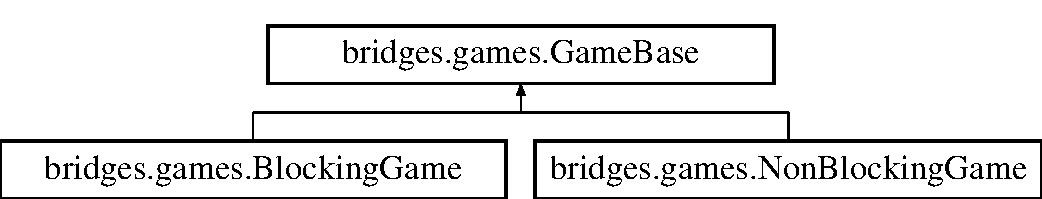
\includegraphics[height=2.000000cm]{classbridges_1_1games_1_1_game_base}
\end{center}
\end{figure}
\subsection*{Public Member Functions}
\begin{DoxyCompactItemize}
\item 
\hyperlink{classbridges_1_1games_1_1_game_base_a9ff11dcae7d4774a6341ff026212f96d}{Game\+Base} (int assid, String login, String apikey, int cols, int rows)
\item 
abstract void \hyperlink{classbridges_1_1games_1_1_game_base_a4b09bc799726e4a59b1ab039b941b188}{start} ()
\begin{DoxyCompactList}\small\item\em Call this function from main to start the game. \end{DoxyCompactList}\end{DoxyCompactItemize}
\subsection*{Protected Member Functions}
\begin{DoxyCompactItemize}
\item 
abstract void \hyperlink{classbridges_1_1games_1_1_game_base_a973a52d5eee7c29b01d668fba3c61657}{initialize} ()
\begin{DoxyCompactList}\small\item\em This function is called once when the game starts. \end{DoxyCompactList}\item 
abstract void \hyperlink{classbridges_1_1games_1_1_game_base_a56d05ed744791cfc1c3792f39ff438f1}{game\+Loop} ()
\begin{DoxyCompactList}\small\item\em This function is called once per frame of the game. \end{DoxyCompactList}\item 
void \hyperlink{classbridges_1_1games_1_1_game_base_aa16a69dc83ee4e32150188e8acf1f897}{quit} ()
\begin{DoxyCompactList}\small\item\em Call this function to stop the game. \end{DoxyCompactList}\item 
void \hyperlink{classbridges_1_1games_1_1_game_base_a9f55e84af9bbf6497b314181c9d79f0a}{set\+Title} (String title)
\begin{DoxyCompactList}\small\item\em Set the title of the game. \end{DoxyCompactList}\item 
void \hyperlink{classbridges_1_1games_1_1_game_base_a3df3bee5b9d32cc9f164d06f9e9707dc}{set\+Description} (String desc)
\begin{DoxyCompactList}\small\item\em Set a short description of the game. \end{DoxyCompactList}\item 
void \hyperlink{classbridges_1_1games_1_1_game_base_ac9a231dd4425eb0f9dea2377653b23c4}{set\+B\+G\+Color} (int x, int y, \hyperlink{enumbridges_1_1base_1_1_named_color}{Named\+Color} c)
\begin{DoxyCompactList}\small\item\em Change the background color of a cell. \end{DoxyCompactList}\item 
\hyperlink{enumbridges_1_1base_1_1_named_color}{Named\+Color} \hyperlink{classbridges_1_1games_1_1_game_base_a516920ad24fefd3118757f0c631b774f}{get\+B\+G\+Color} (int x, int y)
\begin{DoxyCompactList}\small\item\em What color is this cell? \end{DoxyCompactList}\item 
\hyperlink{enumbridges_1_1base_1_1_named_symbol}{Named\+Symbol} \hyperlink{classbridges_1_1games_1_1_game_base_ad7c48a1551044b5f2d0357448cdd3124}{get\+Symbol} (int x, int y)
\begin{DoxyCompactList}\small\item\em What object is in this cell? \end{DoxyCompactList}\item 
\hyperlink{enumbridges_1_1base_1_1_named_color}{Named\+Color} \hyperlink{classbridges_1_1games_1_1_game_base_a07d351db46d88b49471baa68eed23e54}{get\+Symbol\+Color} (int x, int y)
\begin{DoxyCompactList}\small\item\em What color is object in this cell? \end{DoxyCompactList}\item 
void \hyperlink{classbridges_1_1games_1_1_game_base_a7dd4caecd0522dcf7fc275517fbc695d}{draw\+Symbol} (int x, int y, \hyperlink{enumbridges_1_1base_1_1_named_symbol}{Named\+Symbol} s, \hyperlink{enumbridges_1_1base_1_1_named_color}{Named\+Color} c)
\begin{DoxyCompactList}\small\item\em Draw a symbol on the game. \end{DoxyCompactList}\item 
int \hyperlink{classbridges_1_1games_1_1_game_base_a33018840a6f19eb54ef27e55231871f5}{get\+Board\+Width} ()
\begin{DoxyCompactList}\small\item\em How wide is the Game Board? \end{DoxyCompactList}\item 
int \hyperlink{classbridges_1_1games_1_1_game_base_a1effb2a789eb19eb81dec64f25be233e}{get\+Board\+Height} ()
\begin{DoxyCompactList}\small\item\em How tall is the Game Board? \end{DoxyCompactList}\end{DoxyCompactItemize}
\subsection*{Protected Attributes}
\begin{DoxyCompactItemize}
\item 
boolean \hyperlink{classbridges_1_1games_1_1_game_base_acfe2d7adaeac12868e8f4541a6458c26}{debug} = true
\item 
boolean \hyperlink{classbridges_1_1games_1_1_game_base_a762327b538bd37afc7ca58e10f15a42c}{game\+Started} = false
\end{DoxyCompactItemize}


\subsection{Constructor \& Destructor Documentation}
\mbox{\Hypertarget{classbridges_1_1games_1_1_game_base_a9ff11dcae7d4774a6341ff026212f96d}\label{classbridges_1_1games_1_1_game_base_a9ff11dcae7d4774a6341ff026212f96d}} 
\index{bridges\+::games\+::\+Game\+Base@{bridges\+::games\+::\+Game\+Base}!Game\+Base@{Game\+Base}}
\index{Game\+Base@{Game\+Base}!bridges\+::games\+::\+Game\+Base@{bridges\+::games\+::\+Game\+Base}}
\subsubsection{\texorpdfstring{Game\+Base()}{GameBase()}}
{\footnotesize\ttfamily bridges.\+games.\+Game\+Base.\+Game\+Base (\begin{DoxyParamCaption}\item[{int}]{assid,  }\item[{String}]{login,  }\item[{String}]{apikey,  }\item[{int}]{cols,  }\item[{int}]{rows }\end{DoxyParamCaption})}



\subsection{Member Function Documentation}
\mbox{\Hypertarget{classbridges_1_1games_1_1_game_base_a7dd4caecd0522dcf7fc275517fbc695d}\label{classbridges_1_1games_1_1_game_base_a7dd4caecd0522dcf7fc275517fbc695d}} 
\index{bridges\+::games\+::\+Game\+Base@{bridges\+::games\+::\+Game\+Base}!draw\+Symbol@{draw\+Symbol}}
\index{draw\+Symbol@{draw\+Symbol}!bridges\+::games\+::\+Game\+Base@{bridges\+::games\+::\+Game\+Base}}
\subsubsection{\texorpdfstring{draw\+Symbol()}{drawSymbol()}}
{\footnotesize\ttfamily void bridges.\+games.\+Game\+Base.\+draw\+Symbol (\begin{DoxyParamCaption}\item[{int}]{x,  }\item[{int}]{y,  }\item[{\hyperlink{enumbridges_1_1base_1_1_named_symbol}{Named\+Symbol}}]{s,  }\item[{\hyperlink{enumbridges_1_1base_1_1_named_color}{Named\+Color}}]{c }\end{DoxyParamCaption})\hspace{0.3cm}{\ttfamily [protected]}}



Draw a symbol on the game. 


\begin{DoxyParams}{Parameters}
{\em x} & row of the cell to draw the object on \\
\hline
{\em y} & column of the cell to draw the object on \\
\hline
{\em s} & symbol representing the object \\
\hline
{\em c} & color of the object \\
\hline
\end{DoxyParams}
\mbox{\Hypertarget{classbridges_1_1games_1_1_game_base_a56d05ed744791cfc1c3792f39ff438f1}\label{classbridges_1_1games_1_1_game_base_a56d05ed744791cfc1c3792f39ff438f1}} 
\index{bridges\+::games\+::\+Game\+Base@{bridges\+::games\+::\+Game\+Base}!game\+Loop@{game\+Loop}}
\index{game\+Loop@{game\+Loop}!bridges\+::games\+::\+Game\+Base@{bridges\+::games\+::\+Game\+Base}}
\subsubsection{\texorpdfstring{game\+Loop()}{gameLoop()}}
{\footnotesize\ttfamily abstract void bridges.\+games.\+Game\+Base.\+game\+Loop (\begin{DoxyParamCaption}{ }\end{DoxyParamCaption})\hspace{0.3cm}{\ttfamily [abstract]}, {\ttfamily [protected]}}



This function is called once per frame of the game. 

Students write this function. It will be called at each frame of the game. \mbox{\Hypertarget{classbridges_1_1games_1_1_game_base_a516920ad24fefd3118757f0c631b774f}\label{classbridges_1_1games_1_1_game_base_a516920ad24fefd3118757f0c631b774f}} 
\index{bridges\+::games\+::\+Game\+Base@{bridges\+::games\+::\+Game\+Base}!get\+B\+G\+Color@{get\+B\+G\+Color}}
\index{get\+B\+G\+Color@{get\+B\+G\+Color}!bridges\+::games\+::\+Game\+Base@{bridges\+::games\+::\+Game\+Base}}
\subsubsection{\texorpdfstring{get\+B\+G\+Color()}{getBGColor()}}
{\footnotesize\ttfamily \hyperlink{enumbridges_1_1base_1_1_named_color}{Named\+Color} bridges.\+games.\+Game\+Base.\+get\+B\+G\+Color (\begin{DoxyParamCaption}\item[{int}]{x,  }\item[{int}]{y }\end{DoxyParamCaption})\hspace{0.3cm}{\ttfamily [protected]}}



What color is this cell? 


\begin{DoxyParams}{Parameters}
{\em x} & row of the cell \\
\hline
{\em y} & column of the cell \\
\hline
\end{DoxyParams}
\mbox{\Hypertarget{classbridges_1_1games_1_1_game_base_a1effb2a789eb19eb81dec64f25be233e}\label{classbridges_1_1games_1_1_game_base_a1effb2a789eb19eb81dec64f25be233e}} 
\index{bridges\+::games\+::\+Game\+Base@{bridges\+::games\+::\+Game\+Base}!get\+Board\+Height@{get\+Board\+Height}}
\index{get\+Board\+Height@{get\+Board\+Height}!bridges\+::games\+::\+Game\+Base@{bridges\+::games\+::\+Game\+Base}}
\subsubsection{\texorpdfstring{get\+Board\+Height()}{getBoardHeight()}}
{\footnotesize\ttfamily int bridges.\+games.\+Game\+Base.\+get\+Board\+Height (\begin{DoxyParamCaption}{ }\end{DoxyParamCaption})\hspace{0.3cm}{\ttfamily [protected]}}



How tall is the Game Board? 

\begin{DoxyReturn}{Returns}
the number of rows of the board 
\end{DoxyReturn}
\mbox{\Hypertarget{classbridges_1_1games_1_1_game_base_a33018840a6f19eb54ef27e55231871f5}\label{classbridges_1_1games_1_1_game_base_a33018840a6f19eb54ef27e55231871f5}} 
\index{bridges\+::games\+::\+Game\+Base@{bridges\+::games\+::\+Game\+Base}!get\+Board\+Width@{get\+Board\+Width}}
\index{get\+Board\+Width@{get\+Board\+Width}!bridges\+::games\+::\+Game\+Base@{bridges\+::games\+::\+Game\+Base}}
\subsubsection{\texorpdfstring{get\+Board\+Width()}{getBoardWidth()}}
{\footnotesize\ttfamily int bridges.\+games.\+Game\+Base.\+get\+Board\+Width (\begin{DoxyParamCaption}{ }\end{DoxyParamCaption})\hspace{0.3cm}{\ttfamily [protected]}}



How wide is the Game Board? 

\begin{DoxyReturn}{Returns}
the number of columns of the board 
\end{DoxyReturn}
\mbox{\Hypertarget{classbridges_1_1games_1_1_game_base_ad7c48a1551044b5f2d0357448cdd3124}\label{classbridges_1_1games_1_1_game_base_ad7c48a1551044b5f2d0357448cdd3124}} 
\index{bridges\+::games\+::\+Game\+Base@{bridges\+::games\+::\+Game\+Base}!get\+Symbol@{get\+Symbol}}
\index{get\+Symbol@{get\+Symbol}!bridges\+::games\+::\+Game\+Base@{bridges\+::games\+::\+Game\+Base}}
\subsubsection{\texorpdfstring{get\+Symbol()}{getSymbol()}}
{\footnotesize\ttfamily \hyperlink{enumbridges_1_1base_1_1_named_symbol}{Named\+Symbol} bridges.\+games.\+Game\+Base.\+get\+Symbol (\begin{DoxyParamCaption}\item[{int}]{x,  }\item[{int}]{y }\end{DoxyParamCaption})\hspace{0.3cm}{\ttfamily [protected]}}



What object is in this cell? 


\begin{DoxyParams}{Parameters}
{\em x} & row of the cell \\
\hline
{\em y} & column of the cell \\
\hline
\end{DoxyParams}
\mbox{\Hypertarget{classbridges_1_1games_1_1_game_base_a07d351db46d88b49471baa68eed23e54}\label{classbridges_1_1games_1_1_game_base_a07d351db46d88b49471baa68eed23e54}} 
\index{bridges\+::games\+::\+Game\+Base@{bridges\+::games\+::\+Game\+Base}!get\+Symbol\+Color@{get\+Symbol\+Color}}
\index{get\+Symbol\+Color@{get\+Symbol\+Color}!bridges\+::games\+::\+Game\+Base@{bridges\+::games\+::\+Game\+Base}}
\subsubsection{\texorpdfstring{get\+Symbol\+Color()}{getSymbolColor()}}
{\footnotesize\ttfamily \hyperlink{enumbridges_1_1base_1_1_named_color}{Named\+Color} bridges.\+games.\+Game\+Base.\+get\+Symbol\+Color (\begin{DoxyParamCaption}\item[{int}]{x,  }\item[{int}]{y }\end{DoxyParamCaption})\hspace{0.3cm}{\ttfamily [protected]}}



What color is object in this cell? 


\begin{DoxyParams}{Parameters}
{\em x} & row of the cell \\
\hline
{\em y} & column of the cell \\
\hline
\end{DoxyParams}
\mbox{\Hypertarget{classbridges_1_1games_1_1_game_base_a973a52d5eee7c29b01d668fba3c61657}\label{classbridges_1_1games_1_1_game_base_a973a52d5eee7c29b01d668fba3c61657}} 
\index{bridges\+::games\+::\+Game\+Base@{bridges\+::games\+::\+Game\+Base}!initialize@{initialize}}
\index{initialize@{initialize}!bridges\+::games\+::\+Game\+Base@{bridges\+::games\+::\+Game\+Base}}
\subsubsection{\texorpdfstring{initialize()}{initialize()}}
{\footnotesize\ttfamily abstract void bridges.\+games.\+Game\+Base.\+initialize (\begin{DoxyParamCaption}{ }\end{DoxyParamCaption})\hspace{0.3cm}{\ttfamily [abstract]}, {\ttfamily [protected]}}



This function is called once when the game starts. 

Students write this function. It will be called once at the begining of the game. \mbox{\Hypertarget{classbridges_1_1games_1_1_game_base_aa16a69dc83ee4e32150188e8acf1f897}\label{classbridges_1_1games_1_1_game_base_aa16a69dc83ee4e32150188e8acf1f897}} 
\index{bridges\+::games\+::\+Game\+Base@{bridges\+::games\+::\+Game\+Base}!quit@{quit}}
\index{quit@{quit}!bridges\+::games\+::\+Game\+Base@{bridges\+::games\+::\+Game\+Base}}
\subsubsection{\texorpdfstring{quit()}{quit()}}
{\footnotesize\ttfamily void bridges.\+games.\+Game\+Base.\+quit (\begin{DoxyParamCaption}{ }\end{DoxyParamCaption})\hspace{0.3cm}{\ttfamily [protected]}}



Call this function to stop the game. 

\mbox{\Hypertarget{classbridges_1_1games_1_1_game_base_ac9a231dd4425eb0f9dea2377653b23c4}\label{classbridges_1_1games_1_1_game_base_ac9a231dd4425eb0f9dea2377653b23c4}} 
\index{bridges\+::games\+::\+Game\+Base@{bridges\+::games\+::\+Game\+Base}!set\+B\+G\+Color@{set\+B\+G\+Color}}
\index{set\+B\+G\+Color@{set\+B\+G\+Color}!bridges\+::games\+::\+Game\+Base@{bridges\+::games\+::\+Game\+Base}}
\subsubsection{\texorpdfstring{set\+B\+G\+Color()}{setBGColor()}}
{\footnotesize\ttfamily void bridges.\+games.\+Game\+Base.\+set\+B\+G\+Color (\begin{DoxyParamCaption}\item[{int}]{x,  }\item[{int}]{y,  }\item[{\hyperlink{enumbridges_1_1base_1_1_named_color}{Named\+Color}}]{c }\end{DoxyParamCaption})\hspace{0.3cm}{\ttfamily [protected]}}



Change the background color of a cell. 


\begin{DoxyParams}{Parameters}
{\em x} & row of the cell to set \\
\hline
{\em y} & column of the cell to set \\
\hline
{\em c} & Named\+Color to set \\
\hline
\end{DoxyParams}
\mbox{\Hypertarget{classbridges_1_1games_1_1_game_base_a3df3bee5b9d32cc9f164d06f9e9707dc}\label{classbridges_1_1games_1_1_game_base_a3df3bee5b9d32cc9f164d06f9e9707dc}} 
\index{bridges\+::games\+::\+Game\+Base@{bridges\+::games\+::\+Game\+Base}!set\+Description@{set\+Description}}
\index{set\+Description@{set\+Description}!bridges\+::games\+::\+Game\+Base@{bridges\+::games\+::\+Game\+Base}}
\subsubsection{\texorpdfstring{set\+Description()}{setDescription()}}
{\footnotesize\ttfamily void bridges.\+games.\+Game\+Base.\+set\+Description (\begin{DoxyParamCaption}\item[{String}]{desc }\end{DoxyParamCaption})\hspace{0.3cm}{\ttfamily [protected]}}



Set a short description of the game. 


\begin{DoxyParams}{Parameters}
{\em desc} & Description of the game \\
\hline
\end{DoxyParams}
\mbox{\Hypertarget{classbridges_1_1games_1_1_game_base_a9f55e84af9bbf6497b314181c9d79f0a}\label{classbridges_1_1games_1_1_game_base_a9f55e84af9bbf6497b314181c9d79f0a}} 
\index{bridges\+::games\+::\+Game\+Base@{bridges\+::games\+::\+Game\+Base}!set\+Title@{set\+Title}}
\index{set\+Title@{set\+Title}!bridges\+::games\+::\+Game\+Base@{bridges\+::games\+::\+Game\+Base}}
\subsubsection{\texorpdfstring{set\+Title()}{setTitle()}}
{\footnotesize\ttfamily void bridges.\+games.\+Game\+Base.\+set\+Title (\begin{DoxyParamCaption}\item[{String}]{title }\end{DoxyParamCaption})\hspace{0.3cm}{\ttfamily [protected]}}



Set the title of the game. 


\begin{DoxyParams}{Parameters}
{\em title} & Title of the game \\
\hline
\end{DoxyParams}
\mbox{\Hypertarget{classbridges_1_1games_1_1_game_base_a4b09bc799726e4a59b1ab039b941b188}\label{classbridges_1_1games_1_1_game_base_a4b09bc799726e4a59b1ab039b941b188}} 
\index{bridges\+::games\+::\+Game\+Base@{bridges\+::games\+::\+Game\+Base}!start@{start}}
\index{start@{start}!bridges\+::games\+::\+Game\+Base@{bridges\+::games\+::\+Game\+Base}}
\subsubsection{\texorpdfstring{start()}{start()}}
{\footnotesize\ttfamily abstract void bridges.\+games.\+Game\+Base.\+start (\begin{DoxyParamCaption}{ }\end{DoxyParamCaption})\hspace{0.3cm}{\ttfamily [abstract]}}



Call this function from main to start the game. 



\subsection{Member Data Documentation}
\mbox{\Hypertarget{classbridges_1_1games_1_1_game_base_acfe2d7adaeac12868e8f4541a6458c26}\label{classbridges_1_1games_1_1_game_base_acfe2d7adaeac12868e8f4541a6458c26}} 
\index{bridges\+::games\+::\+Game\+Base@{bridges\+::games\+::\+Game\+Base}!debug@{debug}}
\index{debug@{debug}!bridges\+::games\+::\+Game\+Base@{bridges\+::games\+::\+Game\+Base}}
\subsubsection{\texorpdfstring{debug}{debug}}
{\footnotesize\ttfamily boolean bridges.\+games.\+Game\+Base.\+debug = true\hspace{0.3cm}{\ttfamily [protected]}}

\mbox{\Hypertarget{classbridges_1_1games_1_1_game_base_a762327b538bd37afc7ca58e10f15a42c}\label{classbridges_1_1games_1_1_game_base_a762327b538bd37afc7ca58e10f15a42c}} 
\index{bridges\+::games\+::\+Game\+Base@{bridges\+::games\+::\+Game\+Base}!game\+Started@{game\+Started}}
\index{game\+Started@{game\+Started}!bridges\+::games\+::\+Game\+Base@{bridges\+::games\+::\+Game\+Base}}
\subsubsection{\texorpdfstring{game\+Started}{gameStarted}}
{\footnotesize\ttfamily boolean bridges.\+games.\+Game\+Base.\+game\+Started = false\hspace{0.3cm}{\ttfamily [protected]}}



The documentation for this class was generated from the following file\+:\begin{DoxyCompactItemize}
\item 
/home/erik/work/bridges/bridges-\/java/src/main/java/bridges/games/\hyperlink{_game_base_8java}{Game\+Base.\+java}\end{DoxyCompactItemize}

\hypertarget{classbridges_1_1base_1_1_game_cell}{}\doxysection{bridges.\+base.\+Game\+Cell Class Reference}
\label{classbridges_1_1base_1_1_game_cell}\index{bridges.base.GameCell@{bridges.base.GameCell}}


\doxysubsection{Detailed Description}
This class is used to represent cells in Game\+Grids in B\+R\+I\+D\+G\+ES. Each cell has a foreground color, background color, and symbol. 

\begin{DoxyAuthor}{Author}
David Burlinson 
\end{DoxyAuthor}
\begin{DoxyDate}{Date}
9/06/18 
\end{DoxyDate}
\doxysubsection*{Public Member Functions}
\begin{DoxyCompactItemize}
\item 
\mbox{\hyperlink{classbridges_1_1base_1_1_game_cell_a59a4bedeb15c55b71998635520eae21e}{Game\+Cell}} ()
\item 
\mbox{\hyperlink{classbridges_1_1base_1_1_game_cell_aa8c18bc86d5595a6372dbdda66add0fd}{Game\+Cell}} (\mbox{\hyperlink{enumbridges_1_1base_1_1_named_color}{Named\+Color}} bg, \mbox{\hyperlink{enumbridges_1_1base_1_1_named_color}{Named\+Color}} fg, \mbox{\hyperlink{enumbridges_1_1base_1_1_named_symbol}{Named\+Symbol}} symbol)
\item 
void \mbox{\hyperlink{classbridges_1_1base_1_1_game_cell_aa29ae1568daddbc1ca5eec2155385f10}{set\+B\+G\+Color}} (\mbox{\hyperlink{enumbridges_1_1base_1_1_named_color}{Named\+Color}} bg)
\item 
void \mbox{\hyperlink{classbridges_1_1base_1_1_game_cell_af01906e011187218bddf63ddce8c42eb}{set\+F\+G\+Color}} (\mbox{\hyperlink{enumbridges_1_1base_1_1_named_color}{Named\+Color}} fg)
\item 
void \mbox{\hyperlink{classbridges_1_1base_1_1_game_cell_a60805632dec196bfbae6a4de40171447}{set\+B\+G\+Color}} (String bg)
\item 
void \mbox{\hyperlink{classbridges_1_1base_1_1_game_cell_a3ffaf3300d8196a92d46e7c88ae32a86}{set\+F\+G\+Color}} (String fg)
\item 
void \mbox{\hyperlink{classbridges_1_1base_1_1_game_cell_a5e6b4ed374ed3ec4bd6e72723e94848e}{set\+Symbol}} (int s)
\item 
void \mbox{\hyperlink{classbridges_1_1base_1_1_game_cell_a246ba3b4a56f2e440ac21fb0ba297e06}{set\+Symbol}} (\mbox{\hyperlink{enumbridges_1_1base_1_1_named_symbol}{Named\+Symbol}} s)
\item 
\mbox{\hyperlink{enumbridges_1_1base_1_1_named_color}{Named\+Color}} \mbox{\hyperlink{classbridges_1_1base_1_1_game_cell_a7e910723cc5a678ef75f24f993b0c2ca}{get\+B\+G\+Color}} ()
\item 
\mbox{\hyperlink{enumbridges_1_1base_1_1_named_color}{Named\+Color}} \mbox{\hyperlink{classbridges_1_1base_1_1_game_cell_a9355404eb09017ca7ee3e90490e1d13b}{get\+F\+G\+Color}} ()
\item 
\mbox{\hyperlink{enumbridges_1_1base_1_1_named_symbol}{Named\+Symbol}} \mbox{\hyperlink{classbridges_1_1base_1_1_game_cell_a5c5ce5b363e442ac10c8588cbec77511}{get\+Symbol}} ()
\item 
byte \mbox{\hyperlink{classbridges_1_1base_1_1_game_cell_ad431b73e9e0c9e4b0ab539468e8d3a58}{get\+B\+G\+Byte}} ()
\item 
byte \mbox{\hyperlink{classbridges_1_1base_1_1_game_cell_ad1a05ce3e8ca8e148d867e6248023253}{get\+F\+G\+Byte}} ()
\item 
byte \mbox{\hyperlink{classbridges_1_1base_1_1_game_cell_a6b5589c577f2d89c0e98436eea667d77}{get\+Symbol\+Byte}} ()
\end{DoxyCompactItemize}
\doxysubsection*{Static Protected Attributes}
\begin{DoxyCompactItemize}
\item 
static \mbox{\hyperlink{enumbridges_1_1base_1_1_named_symbol}{Named\+Symbol}} \mbox{[}$\,$\mbox{]} \mbox{\hyperlink{classbridges_1_1base_1_1_game_cell_a558b0696aebc6676780316714bf60e0d}{symbol\+Array}} = Named\+Symbol.\+values()
\end{DoxyCompactItemize}


\doxysubsection{Constructor \& Destructor Documentation}
\mbox{\Hypertarget{classbridges_1_1base_1_1_game_cell_a59a4bedeb15c55b71998635520eae21e}\label{classbridges_1_1base_1_1_game_cell_a59a4bedeb15c55b71998635520eae21e}} 
\index{bridges.base.GameCell@{bridges.base.GameCell}!GameCell@{GameCell}}
\index{GameCell@{GameCell}!bridges.base.GameCell@{bridges.base.GameCell}}
\doxysubsubsection{\texorpdfstring{GameCell()}{GameCell()}\hspace{0.1cm}{\footnotesize\ttfamily [1/2]}}
{\footnotesize\ttfamily bridges.\+base.\+Game\+Cell.\+Game\+Cell (\begin{DoxyParamCaption}{ }\end{DoxyParamCaption})}

\mbox{\Hypertarget{classbridges_1_1base_1_1_game_cell_aa8c18bc86d5595a6372dbdda66add0fd}\label{classbridges_1_1base_1_1_game_cell_aa8c18bc86d5595a6372dbdda66add0fd}} 
\index{bridges.base.GameCell@{bridges.base.GameCell}!GameCell@{GameCell}}
\index{GameCell@{GameCell}!bridges.base.GameCell@{bridges.base.GameCell}}
\doxysubsubsection{\texorpdfstring{GameCell()}{GameCell()}\hspace{0.1cm}{\footnotesize\ttfamily [2/2]}}
{\footnotesize\ttfamily bridges.\+base.\+Game\+Cell.\+Game\+Cell (\begin{DoxyParamCaption}\item[{\mbox{\hyperlink{enumbridges_1_1base_1_1_named_color}{Named\+Color}}}]{bg,  }\item[{\mbox{\hyperlink{enumbridges_1_1base_1_1_named_color}{Named\+Color}}}]{fg,  }\item[{\mbox{\hyperlink{enumbridges_1_1base_1_1_named_symbol}{Named\+Symbol}}}]{symbol }\end{DoxyParamCaption})}

Constructor with all arguments specified


\begin{DoxyParams}{Parameters}
{\em bg,fg} & -\/ Named Colors from the \mbox{\hyperlink{enumbridges_1_1base_1_1_named_color}{Named\+Color}} enum \\
\hline
{\em symbol} & -\/ symbol index from range 0-\/255 \\
\hline
\end{DoxyParams}


\doxysubsection{Member Function Documentation}
\mbox{\Hypertarget{classbridges_1_1base_1_1_game_cell_ad431b73e9e0c9e4b0ab539468e8d3a58}\label{classbridges_1_1base_1_1_game_cell_ad431b73e9e0c9e4b0ab539468e8d3a58}} 
\index{bridges.base.GameCell@{bridges.base.GameCell}!getBGByte@{getBGByte}}
\index{getBGByte@{getBGByte}!bridges.base.GameCell@{bridges.base.GameCell}}
\doxysubsubsection{\texorpdfstring{getBGByte()}{getBGByte()}}
{\footnotesize\ttfamily byte bridges.\+base.\+Game\+Cell.\+get\+B\+G\+Byte (\begin{DoxyParamCaption}{ }\end{DoxyParamCaption})}

\begin{DoxyReturn}{Returns}
background color as byte (index of value in \mbox{\hyperlink{enumbridges_1_1base_1_1_named_color}{Named\+Color}}) 
\end{DoxyReturn}
\mbox{\Hypertarget{classbridges_1_1base_1_1_game_cell_a7e910723cc5a678ef75f24f993b0c2ca}\label{classbridges_1_1base_1_1_game_cell_a7e910723cc5a678ef75f24f993b0c2ca}} 
\index{bridges.base.GameCell@{bridges.base.GameCell}!getBGColor@{getBGColor}}
\index{getBGColor@{getBGColor}!bridges.base.GameCell@{bridges.base.GameCell}}
\doxysubsubsection{\texorpdfstring{getBGColor()}{getBGColor()}}
{\footnotesize\ttfamily \mbox{\hyperlink{enumbridges_1_1base_1_1_named_color}{Named\+Color}} bridges.\+base.\+Game\+Cell.\+get\+B\+G\+Color (\begin{DoxyParamCaption}{ }\end{DoxyParamCaption})}

\begin{DoxyReturn}{Returns}
background color 
\end{DoxyReturn}
\mbox{\Hypertarget{classbridges_1_1base_1_1_game_cell_ad1a05ce3e8ca8e148d867e6248023253}\label{classbridges_1_1base_1_1_game_cell_ad1a05ce3e8ca8e148d867e6248023253}} 
\index{bridges.base.GameCell@{bridges.base.GameCell}!getFGByte@{getFGByte}}
\index{getFGByte@{getFGByte}!bridges.base.GameCell@{bridges.base.GameCell}}
\doxysubsubsection{\texorpdfstring{getFGByte()}{getFGByte()}}
{\footnotesize\ttfamily byte bridges.\+base.\+Game\+Cell.\+get\+F\+G\+Byte (\begin{DoxyParamCaption}{ }\end{DoxyParamCaption})}

\begin{DoxyReturn}{Returns}
foreground color as byte (index of value in \mbox{\hyperlink{enumbridges_1_1base_1_1_named_color}{Named\+Color}}) 
\end{DoxyReturn}
\mbox{\Hypertarget{classbridges_1_1base_1_1_game_cell_a9355404eb09017ca7ee3e90490e1d13b}\label{classbridges_1_1base_1_1_game_cell_a9355404eb09017ca7ee3e90490e1d13b}} 
\index{bridges.base.GameCell@{bridges.base.GameCell}!getFGColor@{getFGColor}}
\index{getFGColor@{getFGColor}!bridges.base.GameCell@{bridges.base.GameCell}}
\doxysubsubsection{\texorpdfstring{getFGColor()}{getFGColor()}}
{\footnotesize\ttfamily \mbox{\hyperlink{enumbridges_1_1base_1_1_named_color}{Named\+Color}} bridges.\+base.\+Game\+Cell.\+get\+F\+G\+Color (\begin{DoxyParamCaption}{ }\end{DoxyParamCaption})}

\begin{DoxyReturn}{Returns}
object color 
\end{DoxyReturn}
\mbox{\Hypertarget{classbridges_1_1base_1_1_game_cell_a5c5ce5b363e442ac10c8588cbec77511}\label{classbridges_1_1base_1_1_game_cell_a5c5ce5b363e442ac10c8588cbec77511}} 
\index{bridges.base.GameCell@{bridges.base.GameCell}!getSymbol@{getSymbol}}
\index{getSymbol@{getSymbol}!bridges.base.GameCell@{bridges.base.GameCell}}
\doxysubsubsection{\texorpdfstring{getSymbol()}{getSymbol()}}
{\footnotesize\ttfamily \mbox{\hyperlink{enumbridges_1_1base_1_1_named_symbol}{Named\+Symbol}} bridges.\+base.\+Game\+Cell.\+get\+Symbol (\begin{DoxyParamCaption}{ }\end{DoxyParamCaption})}

\begin{DoxyReturn}{Returns}
symbol 
\end{DoxyReturn}
\mbox{\Hypertarget{classbridges_1_1base_1_1_game_cell_a6b5589c577f2d89c0e98436eea667d77}\label{classbridges_1_1base_1_1_game_cell_a6b5589c577f2d89c0e98436eea667d77}} 
\index{bridges.base.GameCell@{bridges.base.GameCell}!getSymbolByte@{getSymbolByte}}
\index{getSymbolByte@{getSymbolByte}!bridges.base.GameCell@{bridges.base.GameCell}}
\doxysubsubsection{\texorpdfstring{getSymbolByte()}{getSymbolByte()}}
{\footnotesize\ttfamily byte bridges.\+base.\+Game\+Cell.\+get\+Symbol\+Byte (\begin{DoxyParamCaption}{ }\end{DoxyParamCaption})}

\begin{DoxyReturn}{Returns}
symbol as byte 
\end{DoxyReturn}
\mbox{\Hypertarget{classbridges_1_1base_1_1_game_cell_aa29ae1568daddbc1ca5eec2155385f10}\label{classbridges_1_1base_1_1_game_cell_aa29ae1568daddbc1ca5eec2155385f10}} 
\index{bridges.base.GameCell@{bridges.base.GameCell}!setBGColor@{setBGColor}}
\index{setBGColor@{setBGColor}!bridges.base.GameCell@{bridges.base.GameCell}}
\doxysubsubsection{\texorpdfstring{setBGColor()}{setBGColor()}\hspace{0.1cm}{\footnotesize\ttfamily [1/2]}}
{\footnotesize\ttfamily void bridges.\+base.\+Game\+Cell.\+set\+B\+G\+Color (\begin{DoxyParamCaption}\item[{\mbox{\hyperlink{enumbridges_1_1base_1_1_named_color}{Named\+Color}}}]{bg }\end{DoxyParamCaption})}

Set background color using \mbox{\hyperlink{enumbridges_1_1base_1_1_named_color}{Named\+Color}} Enum argument 
\begin{DoxyParams}{Parameters}
{\em bg} & -\/ Named \mbox{\hyperlink{classbridges_1_1base_1_1_color}{Color}} from the \mbox{\hyperlink{enumbridges_1_1base_1_1_named_color}{Named\+Color}} enum \\
\hline
\end{DoxyParams}
\mbox{\Hypertarget{classbridges_1_1base_1_1_game_cell_a60805632dec196bfbae6a4de40171447}\label{classbridges_1_1base_1_1_game_cell_a60805632dec196bfbae6a4de40171447}} 
\index{bridges.base.GameCell@{bridges.base.GameCell}!setBGColor@{setBGColor}}
\index{setBGColor@{setBGColor}!bridges.base.GameCell@{bridges.base.GameCell}}
\doxysubsubsection{\texorpdfstring{setBGColor()}{setBGColor()}\hspace{0.1cm}{\footnotesize\ttfamily [2/2]}}
{\footnotesize\ttfamily void bridges.\+base.\+Game\+Cell.\+set\+B\+G\+Color (\begin{DoxyParamCaption}\item[{String}]{bg }\end{DoxyParamCaption})}

Set background color using String argument 
\begin{DoxyParams}{Parameters}
{\em bg} & -\/ String background color \\
\hline
\end{DoxyParams}
\mbox{\Hypertarget{classbridges_1_1base_1_1_game_cell_af01906e011187218bddf63ddce8c42eb}\label{classbridges_1_1base_1_1_game_cell_af01906e011187218bddf63ddce8c42eb}} 
\index{bridges.base.GameCell@{bridges.base.GameCell}!setFGColor@{setFGColor}}
\index{setFGColor@{setFGColor}!bridges.base.GameCell@{bridges.base.GameCell}}
\doxysubsubsection{\texorpdfstring{setFGColor()}{setFGColor()}\hspace{0.1cm}{\footnotesize\ttfamily [1/2]}}
{\footnotesize\ttfamily void bridges.\+base.\+Game\+Cell.\+set\+F\+G\+Color (\begin{DoxyParamCaption}\item[{\mbox{\hyperlink{enumbridges_1_1base_1_1_named_color}{Named\+Color}}}]{fg }\end{DoxyParamCaption})}

Set foreground color using \mbox{\hyperlink{enumbridges_1_1base_1_1_named_color}{Named\+Color}} Enum argument 
\begin{DoxyParams}{Parameters}
{\em fg} & -\/ Named \mbox{\hyperlink{classbridges_1_1base_1_1_color}{Color}} from the \mbox{\hyperlink{enumbridges_1_1base_1_1_named_color}{Named\+Color}} enum \\
\hline
\end{DoxyParams}
\mbox{\Hypertarget{classbridges_1_1base_1_1_game_cell_a3ffaf3300d8196a92d46e7c88ae32a86}\label{classbridges_1_1base_1_1_game_cell_a3ffaf3300d8196a92d46e7c88ae32a86}} 
\index{bridges.base.GameCell@{bridges.base.GameCell}!setFGColor@{setFGColor}}
\index{setFGColor@{setFGColor}!bridges.base.GameCell@{bridges.base.GameCell}}
\doxysubsubsection{\texorpdfstring{setFGColor()}{setFGColor()}\hspace{0.1cm}{\footnotesize\ttfamily [2/2]}}
{\footnotesize\ttfamily void bridges.\+base.\+Game\+Cell.\+set\+F\+G\+Color (\begin{DoxyParamCaption}\item[{String}]{fg }\end{DoxyParamCaption})}

Set foreground color using String argument 
\begin{DoxyParams}{Parameters}
{\em fg} & -\/ String foreground color \\
\hline
\end{DoxyParams}
\mbox{\Hypertarget{classbridges_1_1base_1_1_game_cell_a5e6b4ed374ed3ec4bd6e72723e94848e}\label{classbridges_1_1base_1_1_game_cell_a5e6b4ed374ed3ec4bd6e72723e94848e}} 
\index{bridges.base.GameCell@{bridges.base.GameCell}!setSymbol@{setSymbol}}
\index{setSymbol@{setSymbol}!bridges.base.GameCell@{bridges.base.GameCell}}
\doxysubsubsection{\texorpdfstring{setSymbol()}{setSymbol()}\hspace{0.1cm}{\footnotesize\ttfamily [1/2]}}
{\footnotesize\ttfamily void bridges.\+base.\+Game\+Cell.\+set\+Symbol (\begin{DoxyParamCaption}\item[{int}]{s }\end{DoxyParamCaption})}

Set symbol using int argument 
\begin{DoxyParams}{Parameters}
{\em s} & -\/ Integer symbol index \\
\hline
\end{DoxyParams}
\mbox{\Hypertarget{classbridges_1_1base_1_1_game_cell_a246ba3b4a56f2e440ac21fb0ba297e06}\label{classbridges_1_1base_1_1_game_cell_a246ba3b4a56f2e440ac21fb0ba297e06}} 
\index{bridges.base.GameCell@{bridges.base.GameCell}!setSymbol@{setSymbol}}
\index{setSymbol@{setSymbol}!bridges.base.GameCell@{bridges.base.GameCell}}
\doxysubsubsection{\texorpdfstring{setSymbol()}{setSymbol()}\hspace{0.1cm}{\footnotesize\ttfamily [2/2]}}
{\footnotesize\ttfamily void bridges.\+base.\+Game\+Cell.\+set\+Symbol (\begin{DoxyParamCaption}\item[{\mbox{\hyperlink{enumbridges_1_1base_1_1_named_symbol}{Named\+Symbol}}}]{s }\end{DoxyParamCaption})}

Set symbol using int argument 
\begin{DoxyParams}{Parameters}
{\em s} & -\/ Named symbol \\
\hline
\end{DoxyParams}


\doxysubsection{Member Data Documentation}
\mbox{\Hypertarget{classbridges_1_1base_1_1_game_cell_a558b0696aebc6676780316714bf60e0d}\label{classbridges_1_1base_1_1_game_cell_a558b0696aebc6676780316714bf60e0d}} 
\index{bridges.base.GameCell@{bridges.base.GameCell}!symbolArray@{symbolArray}}
\index{symbolArray@{symbolArray}!bridges.base.GameCell@{bridges.base.GameCell}}
\doxysubsubsection{\texorpdfstring{symbolArray}{symbolArray}}
{\footnotesize\ttfamily \mbox{\hyperlink{enumbridges_1_1base_1_1_named_symbol}{Named\+Symbol}} \mbox{[}$\,$\mbox{]} bridges.\+base.\+Game\+Cell.\+symbol\+Array = Named\+Symbol.\+values()\hspace{0.3cm}{\ttfamily [static]}, {\ttfamily [protected]}}



The documentation for this class was generated from the following file\+:\begin{DoxyCompactItemize}
\item 
/\+Users/kalpathi/gr/bridges/client/java/src/main/java/bridges/base/\mbox{\hyperlink{_game_cell_8java}{Game\+Cell.\+java}}\end{DoxyCompactItemize}

\hypertarget{classbridges_1_1base_1_1_game_grid}{}\section{bridges.\+base.\+Game\+Grid Class Reference}
\label{classbridges_1_1base_1_1_game_grid}\index{bridges.\+base.\+Game\+Grid@{bridges.\+base.\+Game\+Grid}}
Inheritance diagram for bridges.\+base.\+Game\+Grid\+:\begin{figure}[H]
\begin{center}
\leavevmode
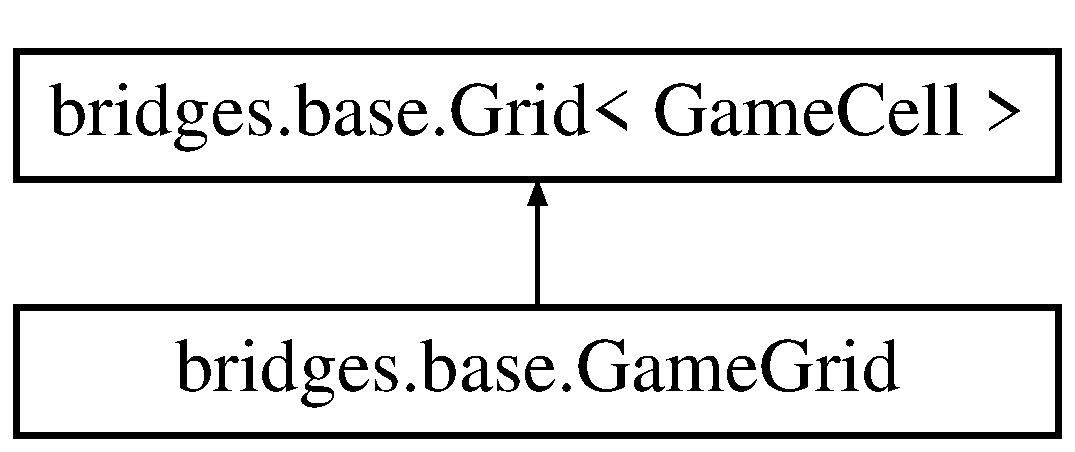
\includegraphics[height=2.000000cm]{classbridges_1_1base_1_1_game_grid}
\end{center}
\end{figure}


\subsection{Detailed Description}
This class in B\+R\+I\+D\+G\+ES is part of the B\+R\+I\+D\+GS Game A\+PI. It is for representing an (m x n) game grid. Each position in the grid will hold a \hyperlink{classbridges_1_1base_1_1_game_cell}{Game\+Cell} object, each of which has a foreground color, background color, and a symbol. 

The A\+PI supports 2D nonblocking games

\begin{DoxyAuthor}{Author}
David Burlinson, Erik Saule 
\end{DoxyAuthor}
\subsection*{Public Member Functions}
\begin{DoxyCompactItemize}
\item 
void \hyperlink{classbridges_1_1base_1_1_game_grid_a2281cfd7d61dc9903c9b1358c9767a1e}{set\+Encoding} (String encoding)
\begin{DoxyCompactList}\small\item\em Enable changing the game grid encoding when building J\+S\+ON representation. \end{DoxyCompactList}\item 
String \hyperlink{classbridges_1_1base_1_1_game_grid_a4d88979ac0f74f212392c5efe1400916}{get\+Data\+Struct\+Type} ()
\begin{DoxyCompactList}\small\item\em Get the data structure type (string) \end{DoxyCompactList}\item 
\hyperlink{classbridges_1_1base_1_1_game_grid_a0b5330e66b504eddc00617c5f1fa6240}{Game\+Grid} ()
\item 
\hyperlink{classbridges_1_1base_1_1_game_grid_acfe6d52979dae94b1d883fed4965feb3}{Game\+Grid} (int rows, int cols)
\item 
void \hyperlink{classbridges_1_1base_1_1_game_grid_a72d7d5b03b78fdc4110cee955727a523}{set\+B\+G\+Color} (Integer row, Integer col, \hyperlink{enumbridges_1_1base_1_1_named_color}{Named\+Color} color)
\item 
\hyperlink{enumbridges_1_1base_1_1_named_color}{Named\+Color} \hyperlink{classbridges_1_1base_1_1_game_grid_abf8435b464054c1f290985b05ce7cd97}{get\+B\+G\+Color} (Integer row, Integer col)
\item 
\hyperlink{enumbridges_1_1base_1_1_named_symbol}{Named\+Symbol} \hyperlink{classbridges_1_1base_1_1_game_grid_a974e33d5561a8f214966be626a9ca8ca}{get\+Symbol} (Integer row, Integer col)
\item 
\hyperlink{enumbridges_1_1base_1_1_named_color}{Named\+Color} \hyperlink{classbridges_1_1base_1_1_game_grid_ab094ebfd585aac9440836ad6875ce094}{get\+Symbol\+Color} (Integer row, Integer col)
\item 
void \hyperlink{classbridges_1_1base_1_1_game_grid_a105b46f68bcc9413889e7255318bab4c}{set\+F\+G\+Color} (Integer row, Integer col, \hyperlink{enumbridges_1_1base_1_1_named_color}{Named\+Color} color)
\item 
void \hyperlink{classbridges_1_1base_1_1_game_grid_ad655bef3f2c24cc19f222b86b5d31373}{set\+B\+G\+Color} (Integer row, Integer col, String color)
\item 
void \hyperlink{classbridges_1_1base_1_1_game_grid_a860f2669ba46bc7691f4bb5c7adf907b}{set\+F\+G\+Color} (Integer row, Integer col, String color)
\item 
void \hyperlink{classbridges_1_1base_1_1_game_grid_a8eee4918e2cbfc956a92a39252590114}{draw\+Symbol} (Integer row, Integer col, Integer symbol)
\item 
void \hyperlink{classbridges_1_1base_1_1_game_grid_a8e8f99d386149e9cd888dd9e6796e5e0}{draw\+Symbol} (Integer row, Integer col, \hyperlink{enumbridges_1_1base_1_1_named_symbol}{Named\+Symbol} symbol)
\item 
void \hyperlink{classbridges_1_1base_1_1_game_grid_a89a27cff9fd390f6d824b7e71534b256}{draw\+Symbol} (Integer row, Integer col, Integer symbol, String color)
\item 
void \hyperlink{classbridges_1_1base_1_1_game_grid_a998fd9e2a9a64e290c9edb01d49f324a}{draw\+Symbol} (Integer row, Integer col, \hyperlink{enumbridges_1_1base_1_1_named_symbol}{Named\+Symbol} symbol, String color)
\item 
void \hyperlink{classbridges_1_1base_1_1_game_grid_ad791794e65de113d96dbd173b34ae820}{draw\+Symbol} (Integer row, Integer col, Integer symbol, \hyperlink{enumbridges_1_1base_1_1_named_color}{Named\+Color} color)
\item 
void \hyperlink{classbridges_1_1base_1_1_game_grid_a778e5b036a18278c9e93e01faa19421c}{draw\+Symbol} (Integer row, Integer col, \hyperlink{enumbridges_1_1base_1_1_named_symbol}{Named\+Symbol} symbol, \hyperlink{enumbridges_1_1base_1_1_named_color}{Named\+Color} color)
\item 
String \hyperlink{classbridges_1_1base_1_1_game_grid_a3c72c7277f9c72ceff82fd063298541e}{get\+Data\+Structure\+Representation} ()
\end{DoxyCompactItemize}
\subsection*{Additional Inherited Members}


\subsection{Constructor \& Destructor Documentation}
\mbox{\Hypertarget{classbridges_1_1base_1_1_game_grid_a0b5330e66b504eddc00617c5f1fa6240}\label{classbridges_1_1base_1_1_game_grid_a0b5330e66b504eddc00617c5f1fa6240}} 
\index{bridges\+::base\+::\+Game\+Grid@{bridges\+::base\+::\+Game\+Grid}!Game\+Grid@{Game\+Grid}}
\index{Game\+Grid@{Game\+Grid}!bridges\+::base\+::\+Game\+Grid@{bridges\+::base\+::\+Game\+Grid}}
\subsubsection{\texorpdfstring{Game\+Grid()}{GameGrid()}\hspace{0.1cm}{\footnotesize\ttfamily [1/2]}}
{\footnotesize\ttfamily bridges.\+base.\+Game\+Grid.\+Game\+Grid (\begin{DoxyParamCaption}{ }\end{DoxyParamCaption})}

Default Game \hyperlink{classbridges_1_1base_1_1_grid}{Grid} constructor Default size is 10 by 10 \mbox{\Hypertarget{classbridges_1_1base_1_1_game_grid_acfe6d52979dae94b1d883fed4965feb3}\label{classbridges_1_1base_1_1_game_grid_acfe6d52979dae94b1d883fed4965feb3}} 
\index{bridges\+::base\+::\+Game\+Grid@{bridges\+::base\+::\+Game\+Grid}!Game\+Grid@{Game\+Grid}}
\index{Game\+Grid@{Game\+Grid}!bridges\+::base\+::\+Game\+Grid@{bridges\+::base\+::\+Game\+Grid}}
\subsubsection{\texorpdfstring{Game\+Grid()}{GameGrid()}\hspace{0.1cm}{\footnotesize\ttfamily [2/2]}}
{\footnotesize\ttfamily bridges.\+base.\+Game\+Grid.\+Game\+Grid (\begin{DoxyParamCaption}\item[{int}]{rows,  }\item[{int}]{cols }\end{DoxyParamCaption})}

\hyperlink{classbridges_1_1base_1_1_grid}{Grid} constructor with grid size arguments


\begin{DoxyParams}{Parameters}
{\em rows} & -\/ int representing the number of rows of the grid \\
\hline
{\em cols} & -\/ int representing the number of columns of the grid \\
\hline
\end{DoxyParams}


\subsection{Member Function Documentation}
\mbox{\Hypertarget{classbridges_1_1base_1_1_game_grid_a8eee4918e2cbfc956a92a39252590114}\label{classbridges_1_1base_1_1_game_grid_a8eee4918e2cbfc956a92a39252590114}} 
\index{bridges\+::base\+::\+Game\+Grid@{bridges\+::base\+::\+Game\+Grid}!draw\+Symbol@{draw\+Symbol}}
\index{draw\+Symbol@{draw\+Symbol}!bridges\+::base\+::\+Game\+Grid@{bridges\+::base\+::\+Game\+Grid}}
\subsubsection{\texorpdfstring{draw\+Symbol()}{drawSymbol()}\hspace{0.1cm}{\footnotesize\ttfamily [1/6]}}
{\footnotesize\ttfamily void bridges.\+base.\+Game\+Grid.\+draw\+Symbol (\begin{DoxyParamCaption}\item[{Integer}]{row,  }\item[{Integer}]{col,  }\item[{Integer}]{symbol }\end{DoxyParamCaption})}

Draw a symbol at the specified location 
\begin{DoxyParams}{Parameters}
{\em row,col} & -\/ integer indices specifying the position to modify \\
\hline
{\em symbol} & -\/ Integer symbol argument to set the symbol at the chosen position \\
\hline
\end{DoxyParams}
\mbox{\Hypertarget{classbridges_1_1base_1_1_game_grid_a8e8f99d386149e9cd888dd9e6796e5e0}\label{classbridges_1_1base_1_1_game_grid_a8e8f99d386149e9cd888dd9e6796e5e0}} 
\index{bridges\+::base\+::\+Game\+Grid@{bridges\+::base\+::\+Game\+Grid}!draw\+Symbol@{draw\+Symbol}}
\index{draw\+Symbol@{draw\+Symbol}!bridges\+::base\+::\+Game\+Grid@{bridges\+::base\+::\+Game\+Grid}}
\subsubsection{\texorpdfstring{draw\+Symbol()}{drawSymbol()}\hspace{0.1cm}{\footnotesize\ttfamily [2/6]}}
{\footnotesize\ttfamily void bridges.\+base.\+Game\+Grid.\+draw\+Symbol (\begin{DoxyParamCaption}\item[{Integer}]{row,  }\item[{Integer}]{col,  }\item[{\hyperlink{enumbridges_1_1base_1_1_named_symbol}{Named\+Symbol}}]{symbol }\end{DoxyParamCaption})}

Draw a symbol at the specified location 
\begin{DoxyParams}{Parameters}
{\em row,col} & -\/ integer indices specifying the position to modify \\
\hline
{\em symbol} & -\/ Named symbol enum argument to set the symbol at the chosen position \\
\hline
\end{DoxyParams}
\mbox{\Hypertarget{classbridges_1_1base_1_1_game_grid_a89a27cff9fd390f6d824b7e71534b256}\label{classbridges_1_1base_1_1_game_grid_a89a27cff9fd390f6d824b7e71534b256}} 
\index{bridges\+::base\+::\+Game\+Grid@{bridges\+::base\+::\+Game\+Grid}!draw\+Symbol@{draw\+Symbol}}
\index{draw\+Symbol@{draw\+Symbol}!bridges\+::base\+::\+Game\+Grid@{bridges\+::base\+::\+Game\+Grid}}
\subsubsection{\texorpdfstring{draw\+Symbol()}{drawSymbol()}\hspace{0.1cm}{\footnotesize\ttfamily [3/6]}}
{\footnotesize\ttfamily void bridges.\+base.\+Game\+Grid.\+draw\+Symbol (\begin{DoxyParamCaption}\item[{Integer}]{row,  }\item[{Integer}]{col,  }\item[{Integer}]{symbol,  }\item[{String}]{color }\end{DoxyParamCaption})}

Draw a symbol at the specified location 
\begin{DoxyParams}{Parameters}
{\em row,col} & -\/ integer indices specifying the position to modify \\
\hline
{\em symbol} & -\/ Integer symbol argument to set the symbol at the chosen position \\
\hline
{\em color} & -\/ String color argument to set the background at the chosen position \\
\hline
\end{DoxyParams}
\mbox{\Hypertarget{classbridges_1_1base_1_1_game_grid_a998fd9e2a9a64e290c9edb01d49f324a}\label{classbridges_1_1base_1_1_game_grid_a998fd9e2a9a64e290c9edb01d49f324a}} 
\index{bridges\+::base\+::\+Game\+Grid@{bridges\+::base\+::\+Game\+Grid}!draw\+Symbol@{draw\+Symbol}}
\index{draw\+Symbol@{draw\+Symbol}!bridges\+::base\+::\+Game\+Grid@{bridges\+::base\+::\+Game\+Grid}}
\subsubsection{\texorpdfstring{draw\+Symbol()}{drawSymbol()}\hspace{0.1cm}{\footnotesize\ttfamily [4/6]}}
{\footnotesize\ttfamily void bridges.\+base.\+Game\+Grid.\+draw\+Symbol (\begin{DoxyParamCaption}\item[{Integer}]{row,  }\item[{Integer}]{col,  }\item[{\hyperlink{enumbridges_1_1base_1_1_named_symbol}{Named\+Symbol}}]{symbol,  }\item[{String}]{color }\end{DoxyParamCaption})}

Draw a symbol at the specified location 
\begin{DoxyParams}{Parameters}
{\em row,col} & -\/ integer indices specifying the position to modify \\
\hline
{\em symbol} & -\/ Named \hyperlink{classbridges_1_1base_1_1_symbol}{Symbol} enum argument to set the symbol at the chosen position \\
\hline
{\em color} & -\/ String color argument to set the background at the chosen position \\
\hline
\end{DoxyParams}
\mbox{\Hypertarget{classbridges_1_1base_1_1_game_grid_ad791794e65de113d96dbd173b34ae820}\label{classbridges_1_1base_1_1_game_grid_ad791794e65de113d96dbd173b34ae820}} 
\index{bridges\+::base\+::\+Game\+Grid@{bridges\+::base\+::\+Game\+Grid}!draw\+Symbol@{draw\+Symbol}}
\index{draw\+Symbol@{draw\+Symbol}!bridges\+::base\+::\+Game\+Grid@{bridges\+::base\+::\+Game\+Grid}}
\subsubsection{\texorpdfstring{draw\+Symbol()}{drawSymbol()}\hspace{0.1cm}{\footnotesize\ttfamily [5/6]}}
{\footnotesize\ttfamily void bridges.\+base.\+Game\+Grid.\+draw\+Symbol (\begin{DoxyParamCaption}\item[{Integer}]{row,  }\item[{Integer}]{col,  }\item[{Integer}]{symbol,  }\item[{\hyperlink{enumbridges_1_1base_1_1_named_color}{Named\+Color}}]{color }\end{DoxyParamCaption})}

Draw a symbol at the specified location 
\begin{DoxyParams}{Parameters}
{\em row,col} & -\/ integer indices specifying the position to modify \\
\hline
{\em symbol} & -\/ Integer symbol argument to set the symbol at the chosen position \\
\hline
{\em color} & -\/ Named \hyperlink{classbridges_1_1base_1_1_color}{Color} enum argument to set the foreground at the chosen position \\
\hline
\end{DoxyParams}
\mbox{\Hypertarget{classbridges_1_1base_1_1_game_grid_a778e5b036a18278c9e93e01faa19421c}\label{classbridges_1_1base_1_1_game_grid_a778e5b036a18278c9e93e01faa19421c}} 
\index{bridges\+::base\+::\+Game\+Grid@{bridges\+::base\+::\+Game\+Grid}!draw\+Symbol@{draw\+Symbol}}
\index{draw\+Symbol@{draw\+Symbol}!bridges\+::base\+::\+Game\+Grid@{bridges\+::base\+::\+Game\+Grid}}
\subsubsection{\texorpdfstring{draw\+Symbol()}{drawSymbol()}\hspace{0.1cm}{\footnotesize\ttfamily [6/6]}}
{\footnotesize\ttfamily void bridges.\+base.\+Game\+Grid.\+draw\+Symbol (\begin{DoxyParamCaption}\item[{Integer}]{row,  }\item[{Integer}]{col,  }\item[{\hyperlink{enumbridges_1_1base_1_1_named_symbol}{Named\+Symbol}}]{symbol,  }\item[{\hyperlink{enumbridges_1_1base_1_1_named_color}{Named\+Color}}]{color }\end{DoxyParamCaption})}

Draw a symbol at the specified location 
\begin{DoxyParams}{Parameters}
{\em row,col} & -\/ integer indices specifying the position to modify \\
\hline
{\em symbol} & -\/ Named \hyperlink{classbridges_1_1base_1_1_symbol}{Symbol} enum argument to set the symbol at the chosen position \\
\hline
{\em color} & -\/ Named \hyperlink{classbridges_1_1base_1_1_color}{Color} enum argument to set the foreground at the chosen position \\
\hline
\end{DoxyParams}
\mbox{\Hypertarget{classbridges_1_1base_1_1_game_grid_abf8435b464054c1f290985b05ce7cd97}\label{classbridges_1_1base_1_1_game_grid_abf8435b464054c1f290985b05ce7cd97}} 
\index{bridges\+::base\+::\+Game\+Grid@{bridges\+::base\+::\+Game\+Grid}!get\+B\+G\+Color@{get\+B\+G\+Color}}
\index{get\+B\+G\+Color@{get\+B\+G\+Color}!bridges\+::base\+::\+Game\+Grid@{bridges\+::base\+::\+Game\+Grid}}
\subsubsection{\texorpdfstring{get\+B\+G\+Color()}{getBGColor()}}
{\footnotesize\ttfamily \hyperlink{enumbridges_1_1base_1_1_named_color}{Named\+Color} bridges.\+base.\+Game\+Grid.\+get\+B\+G\+Color (\begin{DoxyParamCaption}\item[{Integer}]{row,  }\item[{Integer}]{col }\end{DoxyParamCaption})}

Get background color of a cell


\begin{DoxyParams}{Parameters}
{\em row,col} & -\/ integer indices specifying the position\\
\hline
\end{DoxyParams}
\begin{DoxyReturn}{Returns}
background color of cell 
\end{DoxyReturn}
\mbox{\Hypertarget{classbridges_1_1base_1_1_game_grid_a4d88979ac0f74f212392c5efe1400916}\label{classbridges_1_1base_1_1_game_grid_a4d88979ac0f74f212392c5efe1400916}} 
\index{bridges\+::base\+::\+Game\+Grid@{bridges\+::base\+::\+Game\+Grid}!get\+Data\+Struct\+Type@{get\+Data\+Struct\+Type}}
\index{get\+Data\+Struct\+Type@{get\+Data\+Struct\+Type}!bridges\+::base\+::\+Game\+Grid@{bridges\+::base\+::\+Game\+Grid}}
\subsubsection{\texorpdfstring{get\+Data\+Struct\+Type()}{getDataStructType()}}
{\footnotesize\ttfamily String bridges.\+base.\+Game\+Grid.\+get\+Data\+Struct\+Type (\begin{DoxyParamCaption}{ }\end{DoxyParamCaption})}



Get the data structure type (string) 

\begin{DoxyReturn}{Returns}
data structure type 
\end{DoxyReturn}
\mbox{\Hypertarget{classbridges_1_1base_1_1_game_grid_a3c72c7277f9c72ceff82fd063298541e}\label{classbridges_1_1base_1_1_game_grid_a3c72c7277f9c72ceff82fd063298541e}} 
\index{bridges\+::base\+::\+Game\+Grid@{bridges\+::base\+::\+Game\+Grid}!get\+Data\+Structure\+Representation@{get\+Data\+Structure\+Representation}}
\index{get\+Data\+Structure\+Representation@{get\+Data\+Structure\+Representation}!bridges\+::base\+::\+Game\+Grid@{bridges\+::base\+::\+Game\+Grid}}
\subsubsection{\texorpdfstring{get\+Data\+Structure\+Representation()}{getDataStructureRepresentation()}}
{\footnotesize\ttfamily String bridges.\+base.\+Game\+Grid.\+get\+Data\+Structure\+Representation (\begin{DoxyParamCaption}{ }\end{DoxyParamCaption})}

get the J\+S\+ON representation of the game grid. Contains separate foreground, background, and symbol arrays

\begin{DoxyReturn}{Returns}
the J\+S\+ON representation of the game grid 
\end{DoxyReturn}
\mbox{\Hypertarget{classbridges_1_1base_1_1_game_grid_a974e33d5561a8f214966be626a9ca8ca}\label{classbridges_1_1base_1_1_game_grid_a974e33d5561a8f214966be626a9ca8ca}} 
\index{bridges\+::base\+::\+Game\+Grid@{bridges\+::base\+::\+Game\+Grid}!get\+Symbol@{get\+Symbol}}
\index{get\+Symbol@{get\+Symbol}!bridges\+::base\+::\+Game\+Grid@{bridges\+::base\+::\+Game\+Grid}}
\subsubsection{\texorpdfstring{get\+Symbol()}{getSymbol()}}
{\footnotesize\ttfamily \hyperlink{enumbridges_1_1base_1_1_named_symbol}{Named\+Symbol} bridges.\+base.\+Game\+Grid.\+get\+Symbol (\begin{DoxyParamCaption}\item[{Integer}]{row,  }\item[{Integer}]{col }\end{DoxyParamCaption})}

Get symbol at a cell


\begin{DoxyParams}{Parameters}
{\em row,col} & -\/ integer indices specifying the position\\
\hline
\end{DoxyParams}
\begin{DoxyReturn}{Returns}
cell symbol 
\end{DoxyReturn}
\mbox{\Hypertarget{classbridges_1_1base_1_1_game_grid_ab094ebfd585aac9440836ad6875ce094}\label{classbridges_1_1base_1_1_game_grid_ab094ebfd585aac9440836ad6875ce094}} 
\index{bridges\+::base\+::\+Game\+Grid@{bridges\+::base\+::\+Game\+Grid}!get\+Symbol\+Color@{get\+Symbol\+Color}}
\index{get\+Symbol\+Color@{get\+Symbol\+Color}!bridges\+::base\+::\+Game\+Grid@{bridges\+::base\+::\+Game\+Grid}}
\subsubsection{\texorpdfstring{get\+Symbol\+Color()}{getSymbolColor()}}
{\footnotesize\ttfamily \hyperlink{enumbridges_1_1base_1_1_named_color}{Named\+Color} bridges.\+base.\+Game\+Grid.\+get\+Symbol\+Color (\begin{DoxyParamCaption}\item[{Integer}]{row,  }\item[{Integer}]{col }\end{DoxyParamCaption})}

Get symbol color of a cell


\begin{DoxyParams}{Parameters}
{\em row,col} & -\/ integer indices specifying the position\\
\hline
\end{DoxyParams}
\begin{DoxyReturn}{Returns}
cell symbol color 
\end{DoxyReturn}
\mbox{\Hypertarget{classbridges_1_1base_1_1_game_grid_a72d7d5b03b78fdc4110cee955727a523}\label{classbridges_1_1base_1_1_game_grid_a72d7d5b03b78fdc4110cee955727a523}} 
\index{bridges\+::base\+::\+Game\+Grid@{bridges\+::base\+::\+Game\+Grid}!set\+B\+G\+Color@{set\+B\+G\+Color}}
\index{set\+B\+G\+Color@{set\+B\+G\+Color}!bridges\+::base\+::\+Game\+Grid@{bridges\+::base\+::\+Game\+Grid}}
\subsubsection{\texorpdfstring{set\+B\+G\+Color()}{setBGColor()}\hspace{0.1cm}{\footnotesize\ttfamily [1/2]}}
{\footnotesize\ttfamily void bridges.\+base.\+Game\+Grid.\+set\+B\+G\+Color (\begin{DoxyParamCaption}\item[{Integer}]{row,  }\item[{Integer}]{col,  }\item[{\hyperlink{enumbridges_1_1base_1_1_named_color}{Named\+Color}}]{color }\end{DoxyParamCaption})}

Set background color of a cell using an enum argument


\begin{DoxyParams}{Parameters}
{\em row,col} & -\/ integer indices specifying the position to modify \\
\hline
{\em color} & -\/ Named \hyperlink{classbridges_1_1base_1_1_color}{Color} enum argument to set the background at the chosen position \\
\hline
\end{DoxyParams}
\mbox{\Hypertarget{classbridges_1_1base_1_1_game_grid_ad655bef3f2c24cc19f222b86b5d31373}\label{classbridges_1_1base_1_1_game_grid_ad655bef3f2c24cc19f222b86b5d31373}} 
\index{bridges\+::base\+::\+Game\+Grid@{bridges\+::base\+::\+Game\+Grid}!set\+B\+G\+Color@{set\+B\+G\+Color}}
\index{set\+B\+G\+Color@{set\+B\+G\+Color}!bridges\+::base\+::\+Game\+Grid@{bridges\+::base\+::\+Game\+Grid}}
\subsubsection{\texorpdfstring{set\+B\+G\+Color()}{setBGColor()}\hspace{0.1cm}{\footnotesize\ttfamily [2/2]}}
{\footnotesize\ttfamily void bridges.\+base.\+Game\+Grid.\+set\+B\+G\+Color (\begin{DoxyParamCaption}\item[{Integer}]{row,  }\item[{Integer}]{col,  }\item[{String}]{color }\end{DoxyParamCaption})}

Set background color of a cell using an enum argument


\begin{DoxyParams}{Parameters}
{\em row,col} & -\/ integer indices specifying the position to modify \\
\hline
{\em color} & -\/ String color argument to set the background at the chosen position \\
\hline
\end{DoxyParams}
\mbox{\Hypertarget{classbridges_1_1base_1_1_game_grid_a2281cfd7d61dc9903c9b1358c9767a1e}\label{classbridges_1_1base_1_1_game_grid_a2281cfd7d61dc9903c9b1358c9767a1e}} 
\index{bridges\+::base\+::\+Game\+Grid@{bridges\+::base\+::\+Game\+Grid}!set\+Encoding@{set\+Encoding}}
\index{set\+Encoding@{set\+Encoding}!bridges\+::base\+::\+Game\+Grid@{bridges\+::base\+::\+Game\+Grid}}
\subsubsection{\texorpdfstring{set\+Encoding()}{setEncoding()}}
{\footnotesize\ttfamily void bridges.\+base.\+Game\+Grid.\+set\+Encoding (\begin{DoxyParamCaption}\item[{String}]{encoding }\end{DoxyParamCaption})}



Enable changing the game grid encoding when building J\+S\+ON representation. 


\begin{DoxyParams}{Parameters}
{\em encoding} & type of encoding. Supports \char`\"{}raw\char`\"{} and \char`\"{}rle\char`\"{} \\
\hline
\end{DoxyParams}
\mbox{\Hypertarget{classbridges_1_1base_1_1_game_grid_a105b46f68bcc9413889e7255318bab4c}\label{classbridges_1_1base_1_1_game_grid_a105b46f68bcc9413889e7255318bab4c}} 
\index{bridges\+::base\+::\+Game\+Grid@{bridges\+::base\+::\+Game\+Grid}!set\+F\+G\+Color@{set\+F\+G\+Color}}
\index{set\+F\+G\+Color@{set\+F\+G\+Color}!bridges\+::base\+::\+Game\+Grid@{bridges\+::base\+::\+Game\+Grid}}
\subsubsection{\texorpdfstring{set\+F\+G\+Color()}{setFGColor()}\hspace{0.1cm}{\footnotesize\ttfamily [1/2]}}
{\footnotesize\ttfamily void bridges.\+base.\+Game\+Grid.\+set\+F\+G\+Color (\begin{DoxyParamCaption}\item[{Integer}]{row,  }\item[{Integer}]{col,  }\item[{\hyperlink{enumbridges_1_1base_1_1_named_color}{Named\+Color}}]{color }\end{DoxyParamCaption})}

Set foreground color of a cell using an enum argument


\begin{DoxyParams}{Parameters}
{\em row,col} & -\/ integer indices specifying the position to modify \\
\hline
{\em color} & -\/ Named \hyperlink{classbridges_1_1base_1_1_color}{Color} enum argument to set the foreground at the chosen position \\
\hline
\end{DoxyParams}
\mbox{\Hypertarget{classbridges_1_1base_1_1_game_grid_a860f2669ba46bc7691f4bb5c7adf907b}\label{classbridges_1_1base_1_1_game_grid_a860f2669ba46bc7691f4bb5c7adf907b}} 
\index{bridges\+::base\+::\+Game\+Grid@{bridges\+::base\+::\+Game\+Grid}!set\+F\+G\+Color@{set\+F\+G\+Color}}
\index{set\+F\+G\+Color@{set\+F\+G\+Color}!bridges\+::base\+::\+Game\+Grid@{bridges\+::base\+::\+Game\+Grid}}
\subsubsection{\texorpdfstring{set\+F\+G\+Color()}{setFGColor()}\hspace{0.1cm}{\footnotesize\ttfamily [2/2]}}
{\footnotesize\ttfamily void bridges.\+base.\+Game\+Grid.\+set\+F\+G\+Color (\begin{DoxyParamCaption}\item[{Integer}]{row,  }\item[{Integer}]{col,  }\item[{String}]{color }\end{DoxyParamCaption})}

Set foreground color of a cell using an enum argument


\begin{DoxyParams}{Parameters}
{\em row,col} & -\/ integer indices specifying the position to modify \\
\hline
{\em color} & -\/ String color argument to set the foreground at the chosen position \\
\hline
\end{DoxyParams}


The documentation for this class was generated from the following file\+:\begin{DoxyCompactItemize}
\item 
/home/erik/work/bridges/bridges-\/java/src/main/java/bridges/base/\hyperlink{_game_grid_8java}{Game\+Grid.\+java}\end{DoxyCompactItemize}

\hypertarget{classbridges_1_1base_1_1_graph_adj_list}{}\section{bridges.\+base.\+Graph\+Adj\+List$<$ K, E1, E2 $>$ Class Template Reference}
\label{classbridges_1_1base_1_1_graph_adj_list}\index{bridges.\+base.\+Graph\+Adj\+List$<$ K, E1, E2 $>$@{bridges.\+base.\+Graph\+Adj\+List$<$ K, E1, E2 $>$}}
Inheritance diagram for bridges.\+base.\+Graph\+Adj\+List$<$ K, E1, E2 $>$\+:\begin{figure}[H]
\begin{center}
\leavevmode
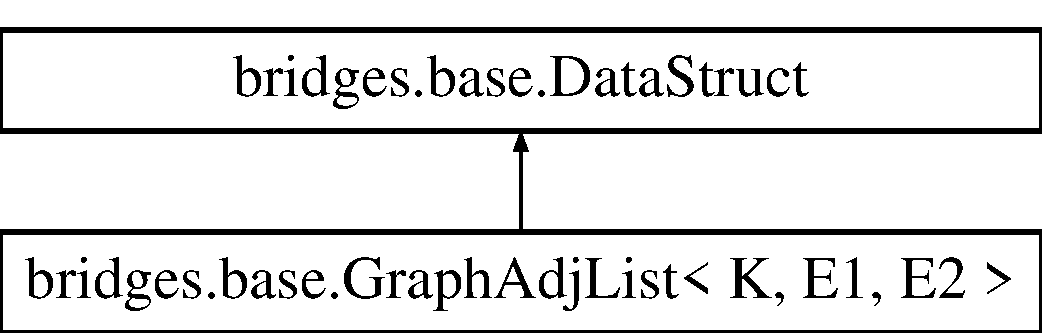
\includegraphics[height=2.000000cm]{classbridges_1_1base_1_1_graph_adj_list}
\end{center}
\end{figure}


\subsection{Detailed Description}
The \hyperlink{classbridges_1_1base_1_1_graph_adj_list}{Graph\+Adj\+List} class can be used to represent adjacency list based graphs in B\+R\+I\+D\+G\+ES. 

The \hyperlink{classbridges_1_1base_1_1_graph_adj_list}{Graph\+Adj\+List} class can be used to represent adjacency list based graphs in B\+R\+I\+D\+G\+ES; it takes 3 generic parameters\+: (1) K, which is an orderable key value used in accessing vertices (in constant time) using a hashmap. This permits data sets that need to be accessed by keys that are strings, (2) E1, for maintaining vertex specific data, and (3) E2, for maintaining edge specific data. The class is a wrapper around the Java Hashmap class and, thus, derives all its operations from it. B\+R\+I\+D\+G\+ES provides methods to visualize the graph and its contents.

The vertices of the graph are held in a Java hashmap, for near constant time access; this enables to use strings or integer ids for vertices. The adjacency lists, also a Java hashmap are built for each vertex and contain the edge (source, destination vertices) in the \hyperlink{classbridges_1_1base_1_1_edge}{Edge} structure, defined separately.

Convenience method \hyperlink{classbridges_1_1base_1_1_graph_adj_list_aca59a3c40af4ae82716ebbfa1751f267}{add\+Vertex()} is provided to add vertices to the graph, and \hyperlink{classbridges_1_1base_1_1_graph_adj_list_a43041976184920e1db1dbe3ad696c6cd}{add\+Edge()} is provided to add edges. Edges are retrieved by using the dual hashmap, given the vertex ids of the edge. Vertices can be styled directly from the vertex element returned by \hyperlink{classbridges_1_1base_1_1_graph_adj_list_aa19cd300a85b05352bdf58720310a112}{get\+Vertex()}, and edges are styled from a \hyperlink{classbridges_1_1base_1_1_link_visualizer}{Link\+Visualizer} one can access through \hyperlink{classbridges_1_1base_1_1_graph_adj_list_af93888dbd2a768a2401619ad5dc95560}{get\+Link\+Visualizer()}. Here is a simple example\+:


\begin{DoxyCode}
GraphAdjList<string, Integer, Double> graph = \textcolor{keyword}{new} GraphAdjList<String, Integer, Double> ();
graph.addVertex(\textcolor{stringliteral}{"a"});
graph.addVertex(\textcolor{stringliteral}{"b"});
graph.addEdge(\textcolor{stringliteral}{"a"}, \textcolor{stringliteral}{"b"});
graph.getVertex(\textcolor{stringliteral}{"a"}).setShape(\textcolor{stringliteral}{"square"});
graph.getLinkVisualizer(\textcolor{stringliteral}{"a"}, \textcolor{stringliteral}{"b"}).setColor(\textcolor{stringliteral}{"yellow"});
\end{DoxyCode}


Adjacency lists are singly linked lists using the B\+R\+I\+D\+G\+ES \hyperlink{classbridges_1_1base_1_1_s_lelement}{S\+Lelement}. Iterators are provided for easy traversal of the adjacency lists. For instance,


\begin{DoxyCode}
GraphAdjList<string, Integer, Double> graph = something();
\textcolor{keywordflow}{for} (Edge<String, Double> e : graph.outgoingEdgeSetOf(\textcolor{stringliteral}{"a"}))
  System.out.println(\textcolor{stringliteral}{"a -> "}+e.getTo());
\end{DoxyCode}


\begin{DoxySeeAlso}{See also}
Example tutorial at \href{http://bridgesuncc.github.io/tutorials/Graph_AL.html}{\tt http\+://bridgesuncc.\+github.\+io/tutorials/\+Graph\+\_\+\+A\+L.\+html}
\end{DoxySeeAlso}
\begin{DoxyAuthor}{Author}
Kalpathi Subramanian, Erik Saule
\end{DoxyAuthor}
\begin{DoxyDate}{Date}
6/29/15, 5/18/17, 4/24/18, 7/14/19
\end{DoxyDate}

\begin{DoxyParams}{Parameters}
{\em K} & orderable key (string, int, etc) that is used to index into vertex \\
\hline
{\em E1} & holds vertex specific information, defined by application \\
\hline
{\em E2} & holds edge specific information, defined by application \\
\hline
\end{DoxyParams}
\subsection*{Public Member Functions}
\begin{DoxyCompactItemize}
\item 
\hyperlink{classbridges_1_1base_1_1_graph_adj_list_aba7e066f43d361418ae6bdf53a23b1de}{Graph\+Adj\+List} ()
\item 
String \hyperlink{classbridges_1_1base_1_1_graph_adj_list_a40c4a2faf20c9847e8ba0d8024236a4b}{get\+Data\+Struct\+Type} ()
\begin{DoxyCompactList}\small\item\em This method gets the data structure type. \end{DoxyCompactList}\item 
void \hyperlink{classbridges_1_1base_1_1_graph_adj_list_aca59a3c40af4ae82716ebbfa1751f267}{add\+Vertex} (K k, E1 e)
\begin{DoxyCompactList}\small\item\em adds a new vertex to the graph. \end{DoxyCompactList}\item 
void \hyperlink{classbridges_1_1base_1_1_graph_adj_list_a43041976184920e1db1dbe3ad696c6cd}{add\+Edge} (K src, K dest)
\begin{DoxyCompactList}\small\item\em adds a new edge to the graph. \end{DoxyCompactList}\item 
void \hyperlink{classbridges_1_1base_1_1_graph_adj_list_aa9fa3cbb6a90de43ee6f0d59c8dce329}{add\+Edge} (K src, K dest, E2 data)
\begin{DoxyCompactList}\small\item\em adds a new edge to the graph. \end{DoxyCompactList}\item 
void \hyperlink{classbridges_1_1base_1_1_graph_adj_list_aa80bfbbe9c4dd130632db1e1165d635e}{set\+Vertex\+Data} (K src, E1 vertex\+\_\+data)
\begin{DoxyCompactList}\small\item\em Sets data for a graph vertex. \end{DoxyCompactList}\item 
E1 \hyperlink{classbridges_1_1base_1_1_graph_adj_list_a3d5f73795bcd5011c425eaca33383454}{get\+Vertex\+Data} (K src)
\begin{DoxyCompactList}\small\item\em Gets data for an edge. \end{DoxyCompactList}\item 
void \hyperlink{classbridges_1_1base_1_1_graph_adj_list_a48041b13b10d5fb677f48a0debfc268e}{set\+Edge\+Data} (K src, K dest, E2 edge\+\_\+data)
\begin{DoxyCompactList}\small\item\em Sets data for an edge. \end{DoxyCompactList}\item 
E2 \hyperlink{classbridges_1_1base_1_1_graph_adj_list_a13cdc7ed89fb211f47e2b04da0b65561}{get\+Edge\+Data} (K src, K dest)
\begin{DoxyCompactList}\small\item\em Gets data for an edge. \end{DoxyCompactList}\item 
Hash\+Map$<$ K, \hyperlink{classbridges_1_1base_1_1_element}{Element}$<$ E1 $>$ $>$ \hyperlink{classbridges_1_1base_1_1_graph_adj_list_acd53b2393db0936ad5812997f67ee1ee}{get\+Vertices} ()
\begin{DoxyCompactList}\small\item\em This method returns the graph vertices. \end{DoxyCompactList}\item 
\hyperlink{classbridges_1_1base_1_1_element}{Element}$<$ E1 $>$ \hyperlink{classbridges_1_1base_1_1_graph_adj_list_aa19cd300a85b05352bdf58720310a112}{get\+Vertex} (K key)
\begin{DoxyCompactList}\small\item\em returns a vertex from its key \end{DoxyCompactList}\item 
Hash\+Map$<$ K, \hyperlink{classbridges_1_1base_1_1_s_lelement}{S\+Lelement}$<$ \hyperlink{classbridges_1_1base_1_1_edge}{Edge}$<$ K, E2 $>$ $>$ $>$ \hyperlink{classbridges_1_1base_1_1_graph_adj_list_a77771e356aa8bf44525be9ae01603989}{get\+Adjacency\+List} ()
\begin{DoxyCompactList}\small\item\em Gets the graph\textquotesingle{}s adjacency list. \end{DoxyCompactList}\item 
\hyperlink{classbridges_1_1base_1_1_s_lelement}{S\+Lelement}$<$ \hyperlink{classbridges_1_1base_1_1_edge}{Edge}$<$ K, E2 $>$ $>$ \hyperlink{classbridges_1_1base_1_1_graph_adj_list_aa8d25bc56b9a172999f0c62ee7e04b6f}{get\+Adjacency\+List} (K vertex)
\begin{DoxyCompactList}\small\item\em Gets the adjacency list of a vertex. \end{DoxyCompactList}\item 
Iterable$<$ \hyperlink{classbridges_1_1base_1_1_edge}{Edge}$<$ K, E2 $>$ $>$ \hyperlink{classbridges_1_1base_1_1_graph_adj_list_a084693f2f464b8f1d21d5ed2a864bf46}{outgoing\+Edge\+Set\+Of} (K vertex)
\begin{DoxyCompactList}\small\item\em returns an iterable set of outgoing edge of a vertex \end{DoxyCompactList}\item 
\hyperlink{classbridges_1_1base_1_1_link_visualizer}{Link\+Visualizer} \hyperlink{classbridges_1_1base_1_1_graph_adj_list_af93888dbd2a768a2401619ad5dc95560}{get\+Link\+Visualizer} (K src, K dest)
\begin{DoxyCompactList}\small\item\em Access a \hyperlink{classbridges_1_1base_1_1_link_visualizer}{Link\+Visualizer} associated with an edge. \end{DoxyCompactList}\item 
\hyperlink{classbridges_1_1base_1_1_element_visualizer}{Element\+Visualizer} \hyperlink{classbridges_1_1base_1_1_graph_adj_list_aafb45833cd5c13b6ce9bdece3fefde6a}{get\+Visualizer} (K vertex)
\begin{DoxyCompactList}\small\item\em Access the \hyperlink{classbridges_1_1base_1_1_element_visualizer}{Element\+Visualizer} associated with a vertex. \end{DoxyCompactList}\item 
void \hyperlink{classbridges_1_1base_1_1_graph_adj_list_a0e2dff032458bb03cb778b571ddcc9b6}{force\+Large\+Visualization} (boolean f)
\begin{DoxyCompactList}\small\item\em Forces the graph use the large graph visualization. \end{DoxyCompactList}\item 
void \hyperlink{classbridges_1_1base_1_1_graph_adj_list_ae14e51214742db0c4dab26c1d409f4ed}{force\+Small\+Visualization} (boolean f)
\begin{DoxyCompactList}\small\item\em Forces the graph to use the small graph visualization. \end{DoxyCompactList}\item 
String \hyperlink{classbridges_1_1base_1_1_graph_adj_list_a9bba66056cdf24197c41fff455e19a6c}{get\+Data\+Structure\+Representation} ()
\end{DoxyCompactItemize}
\subsection*{Additional Inherited Members}


\subsection{Constructor \& Destructor Documentation}
\mbox{\Hypertarget{classbridges_1_1base_1_1_graph_adj_list_aba7e066f43d361418ae6bdf53a23b1de}\label{classbridges_1_1base_1_1_graph_adj_list_aba7e066f43d361418ae6bdf53a23b1de}} 
\index{bridges\+::base\+::\+Graph\+Adj\+List@{bridges\+::base\+::\+Graph\+Adj\+List}!Graph\+Adj\+List@{Graph\+Adj\+List}}
\index{Graph\+Adj\+List@{Graph\+Adj\+List}!bridges\+::base\+::\+Graph\+Adj\+List@{bridges\+::base\+::\+Graph\+Adj\+List}}
\subsubsection{\texorpdfstring{Graph\+Adj\+List()}{GraphAdjList()}}
{\footnotesize\ttfamily \hyperlink{classbridges_1_1base_1_1_graph_adj_list}{bridges.\+base.\+Graph\+Adj\+List}$<$ K, E1, E2 $>$.\hyperlink{classbridges_1_1base_1_1_graph_adj_list}{Graph\+Adj\+List} (\begin{DoxyParamCaption}{ }\end{DoxyParamCaption})}

Constructor 

\subsection{Member Function Documentation}
\mbox{\Hypertarget{classbridges_1_1base_1_1_graph_adj_list_a43041976184920e1db1dbe3ad696c6cd}\label{classbridges_1_1base_1_1_graph_adj_list_a43041976184920e1db1dbe3ad696c6cd}} 
\index{bridges\+::base\+::\+Graph\+Adj\+List@{bridges\+::base\+::\+Graph\+Adj\+List}!add\+Edge@{add\+Edge}}
\index{add\+Edge@{add\+Edge}!bridges\+::base\+::\+Graph\+Adj\+List@{bridges\+::base\+::\+Graph\+Adj\+List}}
\subsubsection{\texorpdfstring{add\+Edge()}{addEdge()}\hspace{0.1cm}{\footnotesize\ttfamily [1/2]}}
{\footnotesize\ttfamily void \hyperlink{classbridges_1_1base_1_1_graph_adj_list}{bridges.\+base.\+Graph\+Adj\+List}$<$ K, E1, E2 $>$.add\+Edge (\begin{DoxyParamCaption}\item[{K}]{src,  }\item[{K}]{dest }\end{DoxyParamCaption})}



adds a new edge to the graph. 

Adds a new edge to the graph, adds it to that vertex\textquotesingle{}s adjacency list; user is responsible for checking if the vertex already exists. This version assumes the edge data is null.


\begin{DoxyParams}{Parameters}
{\em src} & -\/ source vertex of edge \\
\hline
{\em dest} & -\/ destination vertex of edge \\
\hline
\end{DoxyParams}
\mbox{\Hypertarget{classbridges_1_1base_1_1_graph_adj_list_aa9fa3cbb6a90de43ee6f0d59c8dce329}\label{classbridges_1_1base_1_1_graph_adj_list_aa9fa3cbb6a90de43ee6f0d59c8dce329}} 
\index{bridges\+::base\+::\+Graph\+Adj\+List@{bridges\+::base\+::\+Graph\+Adj\+List}!add\+Edge@{add\+Edge}}
\index{add\+Edge@{add\+Edge}!bridges\+::base\+::\+Graph\+Adj\+List@{bridges\+::base\+::\+Graph\+Adj\+List}}
\subsubsection{\texorpdfstring{add\+Edge()}{addEdge()}\hspace{0.1cm}{\footnotesize\ttfamily [2/2]}}
{\footnotesize\ttfamily void \hyperlink{classbridges_1_1base_1_1_graph_adj_list}{bridges.\+base.\+Graph\+Adj\+List}$<$ K, E1, E2 $>$.add\+Edge (\begin{DoxyParamCaption}\item[{K}]{src,  }\item[{K}]{dest,  }\item[{E2}]{data }\end{DoxyParamCaption})}



adds a new edge to the graph. 

Adds a new edge to the graph, adds it to that vertex\textquotesingle{}s adjacency list; user is responsible for checking if the vertex already exists.


\begin{DoxyParams}{Parameters}
{\em src} & -\/ source vertex of edge \\
\hline
{\em dest} & -\/ destination vertex of edge \\
\hline
{\em data} & -\/ edge data \\
\hline
\end{DoxyParams}
\mbox{\Hypertarget{classbridges_1_1base_1_1_graph_adj_list_aca59a3c40af4ae82716ebbfa1751f267}\label{classbridges_1_1base_1_1_graph_adj_list_aca59a3c40af4ae82716ebbfa1751f267}} 
\index{bridges\+::base\+::\+Graph\+Adj\+List@{bridges\+::base\+::\+Graph\+Adj\+List}!add\+Vertex@{add\+Vertex}}
\index{add\+Vertex@{add\+Vertex}!bridges\+::base\+::\+Graph\+Adj\+List@{bridges\+::base\+::\+Graph\+Adj\+List}}
\subsubsection{\texorpdfstring{add\+Vertex()}{addVertex()}}
{\footnotesize\ttfamily void \hyperlink{classbridges_1_1base_1_1_graph_adj_list}{bridges.\+base.\+Graph\+Adj\+List}$<$ K, E1, E2 $>$.add\+Vertex (\begin{DoxyParamCaption}\item[{K}]{k,  }\item[{E1}]{e }\end{DoxyParamCaption})}



adds a new vertex to the graph. 

Adds a new vertex to the graph, initializes the adjacency list; user is responsible for checking if the vertex already exists. This method will replace the value for this key


\begin{DoxyParams}{Parameters}
{\em k} & -\/ vertex id \\
\hline
{\em e} & -\/ vertex info, currently used as a label by default\\
\hline
\end{DoxyParams}
\begin{DoxyReturn}{Returns}
none 
\end{DoxyReturn}
\mbox{\Hypertarget{classbridges_1_1base_1_1_graph_adj_list_a0e2dff032458bb03cb778b571ddcc9b6}\label{classbridges_1_1base_1_1_graph_adj_list_a0e2dff032458bb03cb778b571ddcc9b6}} 
\index{bridges\+::base\+::\+Graph\+Adj\+List@{bridges\+::base\+::\+Graph\+Adj\+List}!force\+Large\+Visualization@{force\+Large\+Visualization}}
\index{force\+Large\+Visualization@{force\+Large\+Visualization}!bridges\+::base\+::\+Graph\+Adj\+List@{bridges\+::base\+::\+Graph\+Adj\+List}}
\subsubsection{\texorpdfstring{force\+Large\+Visualization()}{forceLargeVisualization()}}
{\footnotesize\ttfamily void \hyperlink{classbridges_1_1base_1_1_graph_adj_list}{bridges.\+base.\+Graph\+Adj\+List}$<$ K, E1, E2 $>$.force\+Large\+Visualization (\begin{DoxyParamCaption}\item[{boolean}]{f }\end{DoxyParamCaption})}



Forces the graph use the large graph visualization. 

This forces the rendering is switched to more bandwidth efficient at the cost of having less features. The large graph visualization only renders vertices that have specified locations.


\begin{DoxyParams}{Parameters}
{\em f} & true to force large visualization. \\
\hline
\end{DoxyParams}
\mbox{\Hypertarget{classbridges_1_1base_1_1_graph_adj_list_ae14e51214742db0c4dab26c1d409f4ed}\label{classbridges_1_1base_1_1_graph_adj_list_ae14e51214742db0c4dab26c1d409f4ed}} 
\index{bridges\+::base\+::\+Graph\+Adj\+List@{bridges\+::base\+::\+Graph\+Adj\+List}!force\+Small\+Visualization@{force\+Small\+Visualization}}
\index{force\+Small\+Visualization@{force\+Small\+Visualization}!bridges\+::base\+::\+Graph\+Adj\+List@{bridges\+::base\+::\+Graph\+Adj\+List}}
\subsubsection{\texorpdfstring{force\+Small\+Visualization()}{forceSmallVisualization()}}
{\footnotesize\ttfamily void \hyperlink{classbridges_1_1base_1_1_graph_adj_list}{bridges.\+base.\+Graph\+Adj\+List}$<$ K, E1, E2 $>$.force\+Small\+Visualization (\begin{DoxyParamCaption}\item[{boolean}]{f }\end{DoxyParamCaption})}



Forces the graph to use the small graph visualization. 

The small visualization is use more bandwidth, have more features, and support a force directed layout for vertices which do not have a specified location.


\begin{DoxyParams}{Parameters}
{\em f} & true to force using the small visualization \\
\hline
\end{DoxyParams}
\mbox{\Hypertarget{classbridges_1_1base_1_1_graph_adj_list_a77771e356aa8bf44525be9ae01603989}\label{classbridges_1_1base_1_1_graph_adj_list_a77771e356aa8bf44525be9ae01603989}} 
\index{bridges\+::base\+::\+Graph\+Adj\+List@{bridges\+::base\+::\+Graph\+Adj\+List}!get\+Adjacency\+List@{get\+Adjacency\+List}}
\index{get\+Adjacency\+List@{get\+Adjacency\+List}!bridges\+::base\+::\+Graph\+Adj\+List@{bridges\+::base\+::\+Graph\+Adj\+List}}
\subsubsection{\texorpdfstring{get\+Adjacency\+List()}{getAdjacencyList()}\hspace{0.1cm}{\footnotesize\ttfamily [1/2]}}
{\footnotesize\ttfamily Hash\+Map$<$K, \hyperlink{classbridges_1_1base_1_1_s_lelement}{S\+Lelement}$<$\hyperlink{classbridges_1_1base_1_1_edge}{Edge}$<$K, E2$>$ $>$ $>$ \hyperlink{classbridges_1_1base_1_1_graph_adj_list}{bridges.\+base.\+Graph\+Adj\+List}$<$ K, E1, E2 $>$.get\+Adjacency\+List (\begin{DoxyParamCaption}{ }\end{DoxyParamCaption})}



Gets the graph\textquotesingle{}s adjacency list. 

\begin{DoxyReturn}{Returns}
the graph\textquotesingle{}s adjacency lists 
\end{DoxyReturn}
\mbox{\Hypertarget{classbridges_1_1base_1_1_graph_adj_list_aa8d25bc56b9a172999f0c62ee7e04b6f}\label{classbridges_1_1base_1_1_graph_adj_list_aa8d25bc56b9a172999f0c62ee7e04b6f}} 
\index{bridges\+::base\+::\+Graph\+Adj\+List@{bridges\+::base\+::\+Graph\+Adj\+List}!get\+Adjacency\+List@{get\+Adjacency\+List}}
\index{get\+Adjacency\+List@{get\+Adjacency\+List}!bridges\+::base\+::\+Graph\+Adj\+List@{bridges\+::base\+::\+Graph\+Adj\+List}}
\subsubsection{\texorpdfstring{get\+Adjacency\+List()}{getAdjacencyList()}\hspace{0.1cm}{\footnotesize\ttfamily [2/2]}}
{\footnotesize\ttfamily \hyperlink{classbridges_1_1base_1_1_s_lelement}{S\+Lelement}$<$\hyperlink{classbridges_1_1base_1_1_edge}{Edge}$<$K, E2$>$ $>$ \hyperlink{classbridges_1_1base_1_1_graph_adj_list}{bridges.\+base.\+Graph\+Adj\+List}$<$ K, E1, E2 $>$.get\+Adjacency\+List (\begin{DoxyParamCaption}\item[{K}]{vertex }\end{DoxyParamCaption})}



Gets the adjacency list of a vertex. 


\begin{DoxyParams}{Parameters}
{\em vertex} & the key of the vertex\\
\hline
\end{DoxyParams}
\begin{DoxyReturn}{Returns}
-\/ the graph\textquotesingle{}s adjacency list corresponding to this vertex 
\end{DoxyReturn}
\mbox{\Hypertarget{classbridges_1_1base_1_1_graph_adj_list_a40c4a2faf20c9847e8ba0d8024236a4b}\label{classbridges_1_1base_1_1_graph_adj_list_a40c4a2faf20c9847e8ba0d8024236a4b}} 
\index{bridges\+::base\+::\+Graph\+Adj\+List@{bridges\+::base\+::\+Graph\+Adj\+List}!get\+Data\+Struct\+Type@{get\+Data\+Struct\+Type}}
\index{get\+Data\+Struct\+Type@{get\+Data\+Struct\+Type}!bridges\+::base\+::\+Graph\+Adj\+List@{bridges\+::base\+::\+Graph\+Adj\+List}}
\subsubsection{\texorpdfstring{get\+Data\+Struct\+Type()}{getDataStructType()}}
{\footnotesize\ttfamily String \hyperlink{classbridges_1_1base_1_1_graph_adj_list}{bridges.\+base.\+Graph\+Adj\+List}$<$ K, E1, E2 $>$.get\+Data\+Struct\+Type (\begin{DoxyParamCaption}{ }\end{DoxyParamCaption})}



This method gets the data structure type. 

\begin{DoxyReturn}{Returns}
The date structure type as a string 
\end{DoxyReturn}
\mbox{\Hypertarget{classbridges_1_1base_1_1_graph_adj_list_a9bba66056cdf24197c41fff455e19a6c}\label{classbridges_1_1base_1_1_graph_adj_list_a9bba66056cdf24197c41fff455e19a6c}} 
\index{bridges\+::base\+::\+Graph\+Adj\+List@{bridges\+::base\+::\+Graph\+Adj\+List}!get\+Data\+Structure\+Representation@{get\+Data\+Structure\+Representation}}
\index{get\+Data\+Structure\+Representation@{get\+Data\+Structure\+Representation}!bridges\+::base\+::\+Graph\+Adj\+List@{bridges\+::base\+::\+Graph\+Adj\+List}}
\subsubsection{\texorpdfstring{get\+Data\+Structure\+Representation()}{getDataStructureRepresentation()}}
{\footnotesize\ttfamily String \hyperlink{classbridges_1_1base_1_1_graph_adj_list}{bridges.\+base.\+Graph\+Adj\+List}$<$ K, E1, E2 $>$.get\+Data\+Structure\+Representation (\begin{DoxyParamCaption}{ }\end{DoxyParamCaption})}

\mbox{\Hypertarget{classbridges_1_1base_1_1_graph_adj_list_a13cdc7ed89fb211f47e2b04da0b65561}\label{classbridges_1_1base_1_1_graph_adj_list_a13cdc7ed89fb211f47e2b04da0b65561}} 
\index{bridges\+::base\+::\+Graph\+Adj\+List@{bridges\+::base\+::\+Graph\+Adj\+List}!get\+Edge\+Data@{get\+Edge\+Data}}
\index{get\+Edge\+Data@{get\+Edge\+Data}!bridges\+::base\+::\+Graph\+Adj\+List@{bridges\+::base\+::\+Graph\+Adj\+List}}
\subsubsection{\texorpdfstring{get\+Edge\+Data()}{getEdgeData()}}
{\footnotesize\ttfamily E2 \hyperlink{classbridges_1_1base_1_1_graph_adj_list}{bridges.\+base.\+Graph\+Adj\+List}$<$ K, E1, E2 $>$.get\+Edge\+Data (\begin{DoxyParamCaption}\item[{K}]{src,  }\item[{K}]{dest }\end{DoxyParamCaption})}



Gets data for an edge. 


\begin{DoxyParams}{Parameters}
{\em src} & source vertex of edge \\
\hline
{\em dest} & destination vertex of edge\\
\hline
\end{DoxyParams}
\begin{DoxyReturn}{Returns}
the edge data, or null if the edge does not exist 
\end{DoxyReturn}
\mbox{\Hypertarget{classbridges_1_1base_1_1_graph_adj_list_af93888dbd2a768a2401619ad5dc95560}\label{classbridges_1_1base_1_1_graph_adj_list_af93888dbd2a768a2401619ad5dc95560}} 
\index{bridges\+::base\+::\+Graph\+Adj\+List@{bridges\+::base\+::\+Graph\+Adj\+List}!get\+Link\+Visualizer@{get\+Link\+Visualizer}}
\index{get\+Link\+Visualizer@{get\+Link\+Visualizer}!bridges\+::base\+::\+Graph\+Adj\+List@{bridges\+::base\+::\+Graph\+Adj\+List}}
\subsubsection{\texorpdfstring{get\+Link\+Visualizer()}{getLinkVisualizer()}}
{\footnotesize\ttfamily \hyperlink{classbridges_1_1base_1_1_link_visualizer}{Link\+Visualizer} \hyperlink{classbridges_1_1base_1_1_graph_adj_list}{bridges.\+base.\+Graph\+Adj\+List}$<$ K, E1, E2 $>$.get\+Link\+Visualizer (\begin{DoxyParamCaption}\item[{K}]{src,  }\item[{K}]{dest }\end{DoxyParamCaption})}



Access a \hyperlink{classbridges_1_1base_1_1_link_visualizer}{Link\+Visualizer} associated with an edge. 

This is a convenience method to simplify access to the link visualizer; the method assumes the vertex names point to existing vertices, else an exception is thrown


\begin{DoxyParams}{Parameters}
{\em src} & source vertex \\
\hline
{\em dest} & destination vertex\\
\hline
\end{DoxyParams}
\begin{DoxyReturn}{Returns}
the \hyperlink{classbridges_1_1base_1_1_link_visualizer}{Link\+Visualizer} of an edge from src to dest, or null if the edge does not exist 
\end{DoxyReturn}
\mbox{\Hypertarget{classbridges_1_1base_1_1_graph_adj_list_aa19cd300a85b05352bdf58720310a112}\label{classbridges_1_1base_1_1_graph_adj_list_aa19cd300a85b05352bdf58720310a112}} 
\index{bridges\+::base\+::\+Graph\+Adj\+List@{bridges\+::base\+::\+Graph\+Adj\+List}!get\+Vertex@{get\+Vertex}}
\index{get\+Vertex@{get\+Vertex}!bridges\+::base\+::\+Graph\+Adj\+List@{bridges\+::base\+::\+Graph\+Adj\+List}}
\subsubsection{\texorpdfstring{get\+Vertex()}{getVertex()}}
{\footnotesize\ttfamily \hyperlink{classbridges_1_1base_1_1_element}{Element}$<$E1$>$ \hyperlink{classbridges_1_1base_1_1_graph_adj_list}{bridges.\+base.\+Graph\+Adj\+List}$<$ K, E1, E2 $>$.get\+Vertex (\begin{DoxyParamCaption}\item[{K}]{key }\end{DoxyParamCaption})}



returns a vertex from its key 

This is a convenience method to retrieve a vertex given its key

\begin{DoxyReturn}{Returns}
graph vertex corresponding to its key 
\end{DoxyReturn}
\mbox{\Hypertarget{classbridges_1_1base_1_1_graph_adj_list_a3d5f73795bcd5011c425eaca33383454}\label{classbridges_1_1base_1_1_graph_adj_list_a3d5f73795bcd5011c425eaca33383454}} 
\index{bridges\+::base\+::\+Graph\+Adj\+List@{bridges\+::base\+::\+Graph\+Adj\+List}!get\+Vertex\+Data@{get\+Vertex\+Data}}
\index{get\+Vertex\+Data@{get\+Vertex\+Data}!bridges\+::base\+::\+Graph\+Adj\+List@{bridges\+::base\+::\+Graph\+Adj\+List}}
\subsubsection{\texorpdfstring{get\+Vertex\+Data()}{getVertexData()}}
{\footnotesize\ttfamily E1 \hyperlink{classbridges_1_1base_1_1_graph_adj_list}{bridges.\+base.\+Graph\+Adj\+List}$<$ K, E1, E2 $>$.get\+Vertex\+Data (\begin{DoxyParamCaption}\item[{K}]{src }\end{DoxyParamCaption})}



Gets data for an edge. 


\begin{DoxyParams}{Parameters}
{\em src} & -\/ source vertex of edge \\
\hline
\end{DoxyParams}
\mbox{\Hypertarget{classbridges_1_1base_1_1_graph_adj_list_acd53b2393db0936ad5812997f67ee1ee}\label{classbridges_1_1base_1_1_graph_adj_list_acd53b2393db0936ad5812997f67ee1ee}} 
\index{bridges\+::base\+::\+Graph\+Adj\+List@{bridges\+::base\+::\+Graph\+Adj\+List}!get\+Vertices@{get\+Vertices}}
\index{get\+Vertices@{get\+Vertices}!bridges\+::base\+::\+Graph\+Adj\+List@{bridges\+::base\+::\+Graph\+Adj\+List}}
\subsubsection{\texorpdfstring{get\+Vertices()}{getVertices()}}
{\footnotesize\ttfamily Hash\+Map$<$K, \hyperlink{classbridges_1_1base_1_1_element}{Element}$<$E1$>$ $>$ \hyperlink{classbridges_1_1base_1_1_graph_adj_list}{bridges.\+base.\+Graph\+Adj\+List}$<$ K, E1, E2 $>$.get\+Vertices (\begin{DoxyParamCaption}{ }\end{DoxyParamCaption})}



This method returns the graph vertices. 

\begin{DoxyReturn}{Returns}
vertices held in the hashmap 
\end{DoxyReturn}
\mbox{\Hypertarget{classbridges_1_1base_1_1_graph_adj_list_aafb45833cd5c13b6ce9bdece3fefde6a}\label{classbridges_1_1base_1_1_graph_adj_list_aafb45833cd5c13b6ce9bdece3fefde6a}} 
\index{bridges\+::base\+::\+Graph\+Adj\+List@{bridges\+::base\+::\+Graph\+Adj\+List}!get\+Visualizer@{get\+Visualizer}}
\index{get\+Visualizer@{get\+Visualizer}!bridges\+::base\+::\+Graph\+Adj\+List@{bridges\+::base\+::\+Graph\+Adj\+List}}
\subsubsection{\texorpdfstring{get\+Visualizer()}{getVisualizer()}}
{\footnotesize\ttfamily \hyperlink{classbridges_1_1base_1_1_element_visualizer}{Element\+Visualizer} \hyperlink{classbridges_1_1base_1_1_graph_adj_list}{bridges.\+base.\+Graph\+Adj\+List}$<$ K, E1, E2 $>$.get\+Visualizer (\begin{DoxyParamCaption}\item[{K}]{vertex }\end{DoxyParamCaption})}



Access the \hyperlink{classbridges_1_1base_1_1_element_visualizer}{Element\+Visualizer} associated with a vertex. 

This is a convenience method to simplify access to the element visualizer; the method assumes the vertex name points to an existing vertice, else an exception is thrown


\begin{DoxyParams}{Parameters}
{\em vertex} & graph vertex \\
\hline
\end{DoxyParams}
\begin{DoxyReturn}{Returns}
the element visualizer of this vertex 
\end{DoxyReturn}
\mbox{\Hypertarget{classbridges_1_1base_1_1_graph_adj_list_a084693f2f464b8f1d21d5ed2a864bf46}\label{classbridges_1_1base_1_1_graph_adj_list_a084693f2f464b8f1d21d5ed2a864bf46}} 
\index{bridges\+::base\+::\+Graph\+Adj\+List@{bridges\+::base\+::\+Graph\+Adj\+List}!outgoing\+Edge\+Set\+Of@{outgoing\+Edge\+Set\+Of}}
\index{outgoing\+Edge\+Set\+Of@{outgoing\+Edge\+Set\+Of}!bridges\+::base\+::\+Graph\+Adj\+List@{bridges\+::base\+::\+Graph\+Adj\+List}}
\subsubsection{\texorpdfstring{outgoing\+Edge\+Set\+Of()}{outgoingEdgeSetOf()}}
{\footnotesize\ttfamily Iterable$<$\hyperlink{classbridges_1_1base_1_1_edge}{Edge}$<$K, E2$>$ $>$ \hyperlink{classbridges_1_1base_1_1_graph_adj_list}{bridges.\+base.\+Graph\+Adj\+List}$<$ K, E1, E2 $>$.outgoing\+Edge\+Set\+Of (\begin{DoxyParamCaption}\item[{K}]{vertex }\end{DoxyParamCaption})}



returns an iterable set of outgoing edge of a vertex 

Gets a vector of the outgoing edges from a graph vertex 
\begin{DoxyParams}{Parameters}
{\em vertex} & vertex identifier \\
\hline
\end{DoxyParams}
\begin{DoxyReturn}{Returns}
an iterable set of the outgoing edge of this vertex 
\end{DoxyReturn}
\mbox{\Hypertarget{classbridges_1_1base_1_1_graph_adj_list_a48041b13b10d5fb677f48a0debfc268e}\label{classbridges_1_1base_1_1_graph_adj_list_a48041b13b10d5fb677f48a0debfc268e}} 
\index{bridges\+::base\+::\+Graph\+Adj\+List@{bridges\+::base\+::\+Graph\+Adj\+List}!set\+Edge\+Data@{set\+Edge\+Data}}
\index{set\+Edge\+Data@{set\+Edge\+Data}!bridges\+::base\+::\+Graph\+Adj\+List@{bridges\+::base\+::\+Graph\+Adj\+List}}
\subsubsection{\texorpdfstring{set\+Edge\+Data()}{setEdgeData()}}
{\footnotesize\ttfamily void \hyperlink{classbridges_1_1base_1_1_graph_adj_list}{bridges.\+base.\+Graph\+Adj\+List}$<$ K, E1, E2 $>$.set\+Edge\+Data (\begin{DoxyParamCaption}\item[{K}]{src,  }\item[{K}]{dest,  }\item[{E2}]{edge\+\_\+data }\end{DoxyParamCaption})}



Sets data for an edge. 


\begin{DoxyParams}{Parameters}
{\em src} & -\/ source vertex of edge \\
\hline
{\em dest} & -\/ destination vertex of edge \\
\hline
{\em edge\+\_\+data} & -\/ edge data \\
\hline
\end{DoxyParams}
\mbox{\Hypertarget{classbridges_1_1base_1_1_graph_adj_list_aa80bfbbe9c4dd130632db1e1165d635e}\label{classbridges_1_1base_1_1_graph_adj_list_aa80bfbbe9c4dd130632db1e1165d635e}} 
\index{bridges\+::base\+::\+Graph\+Adj\+List@{bridges\+::base\+::\+Graph\+Adj\+List}!set\+Vertex\+Data@{set\+Vertex\+Data}}
\index{set\+Vertex\+Data@{set\+Vertex\+Data}!bridges\+::base\+::\+Graph\+Adj\+List@{bridges\+::base\+::\+Graph\+Adj\+List}}
\subsubsection{\texorpdfstring{set\+Vertex\+Data()}{setVertexData()}}
{\footnotesize\ttfamily void \hyperlink{classbridges_1_1base_1_1_graph_adj_list}{bridges.\+base.\+Graph\+Adj\+List}$<$ K, E1, E2 $>$.set\+Vertex\+Data (\begin{DoxyParamCaption}\item[{K}]{src,  }\item[{E1}]{vertex\+\_\+data }\end{DoxyParamCaption})}



Sets data for a graph vertex. 


\begin{DoxyParams}{Parameters}
{\em src} & source vertex of edge \\
\hline
{\em vertex\+\_\+data} & vertex data \\
\hline
\end{DoxyParams}


The documentation for this class was generated from the following file\+:\begin{DoxyCompactItemize}
\item 
/home/erik/work/bridges/bridges-\/java/src/main/java/bridges/base/\hyperlink{_graph_adj_list_8java}{Graph\+Adj\+List.\+java}\end{DoxyCompactItemize}

\hypertarget{classbridges_1_1base_1_1_graph_adj_list_simple}{}\section{bridges.\+base.\+Graph\+Adj\+List\+Simple$<$ K $>$ Class Template Reference}
\label{classbridges_1_1base_1_1_graph_adj_list_simple}\index{bridges.\+base.\+Graph\+Adj\+List\+Simple$<$ K $>$@{bridges.\+base.\+Graph\+Adj\+List\+Simple$<$ K $>$}}


The \hyperlink{classbridges_1_1base_1_1_graph_adj_list_simple}{Graph\+Adj\+List\+Simple} class is a simplification of the \hyperlink{classbridges_1_1base_1_1_graph_adj_list}{Graph\+Adj\+List} class; this class is useful in applications where vertex and edge specific information is not used; this class is thus a specialization of \hyperlink{classbridges_1_1base_1_1_graph_adj_list}{Graph\+Adj\+List} with only a single generic parameter that specifies the key type.  


Inheritance diagram for bridges.\+base.\+Graph\+Adj\+List\+Simple$<$ K $>$\+:\begin{figure}[H]
\begin{center}
\leavevmode
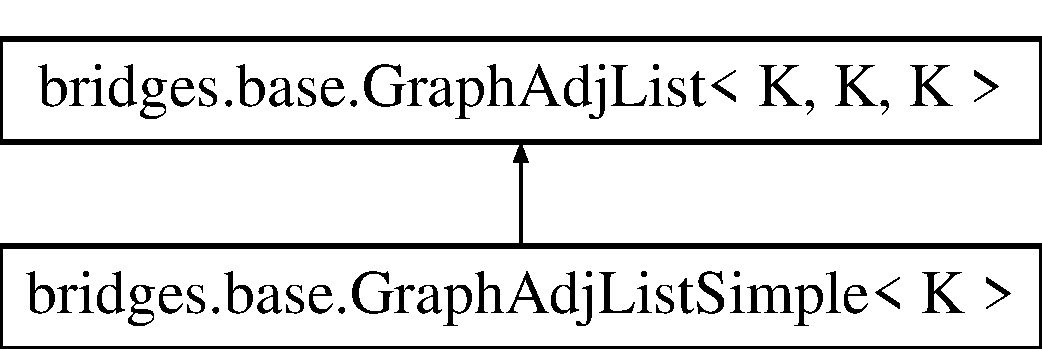
\includegraphics[height=2.000000cm]{classbridges_1_1base_1_1_graph_adj_list_simple}
\end{center}
\end{figure}
\subsection*{Additional Inherited Members}


\subsection{Detailed Description}
The \hyperlink{classbridges_1_1base_1_1_graph_adj_list_simple}{Graph\+Adj\+List\+Simple} class is a simplification of the \hyperlink{classbridges_1_1base_1_1_graph_adj_list}{Graph\+Adj\+List} class; this class is useful in applications where vertex and edge specific information is not used; this class is thus a specialization of \hyperlink{classbridges_1_1base_1_1_graph_adj_list}{Graph\+Adj\+List} with only a single generic parameter that specifies the key type. 

The \hyperlink{classbridges_1_1base_1_1_graph_adj_list_simple}{Graph\+Adj\+List\+Simple} class can be used to represent adjacency list based graphs in B\+R\+I\+D\+G\+E\+S; it takes 1 generic parameter\+: K, which is an orderable key value used in accessing vertices and edges (in constant time) using hashmaps. This permits data sets that need to be accessed by keys that are strings. Vertex and edge specific information can still be represented, but they will be restricted to be of type K.

The class is simply a wrapper around the Java Hashmap class and, thus, derives all its operations from it. B\+R\+I\+D\+G\+E\+S provides methods to visualize the graph and its contents.

The vertices of the graph are held in a Java hashmap, for near constant time access; this lets us use strings or integral ids for vertices. The adjacency lists, also a Java hashmap are built for each vertex and contain the edge (terminating vertex id, weight) in the \hyperlink{classbridges_1_1base_1_1_edge}{Edge} structure, defined separately. Adjacency lists are singly linked lists using the B\+R\+I\+D\+G\+E\+S \hyperlink{classbridges_1_1base_1_1_s_lelement}{S\+Lelement}.

Convenience methods are provided to add vertices and edges to the graph as well as retrieve the adjacency list of a vertex, given its id. Methods to access and set visual attributes are also provided, indexed by the vertex ids.

\begin{DoxyAuthor}{Author}
Kalpathi Subramanian
\end{DoxyAuthor}
\begin{DoxyDate}{Date}
4/24/18
\end{DoxyDate}

\begin{DoxyParams}{Parameters}
{\em $<$\+K$>$} & orderable key (string, int, etc) that is used to index into vertex\\
\hline
\end{DoxyParams}
\begin{DoxySeeAlso}{See also}
Example tutorial at 
\end{DoxySeeAlso}
\href{http://bridgesuncc.github.io/Hello_World_Tutorials/Graph.html}{\tt http\+://bridgesuncc.\+github.\+io/\+Hello\+\_\+\+World\+\_\+\+Tutorials/\+Graph.\+html} 

The documentation for this class was generated from the following file\+:\begin{DoxyCompactItemize}
\item 
/\+Users/kalpathi/gr/bridges/bridges17/java/src/main/java/bridges/base/\hyperlink{_graph_adj_list_simple_8java}{Graph\+Adj\+List\+Simple.\+java}\end{DoxyCompactItemize}

\hypertarget{classbridges_1_1base_1_1_graph_adj_matrix}{}\section{bridges.\+base.\+Graph\+Adj\+Matrix$<$ K, E1, E2 $>$ Class Template Reference}
\label{classbridges_1_1base_1_1_graph_adj_matrix}\index{bridges.\+base.\+Graph\+Adj\+Matrix$<$ K, E1, E2 $>$@{bridges.\+base.\+Graph\+Adj\+Matrix$<$ K, E1, E2 $>$}}
Inheritance diagram for bridges.\+base.\+Graph\+Adj\+Matrix$<$ K, E1, E2 $>$\+:\begin{figure}[H]
\begin{center}
\leavevmode
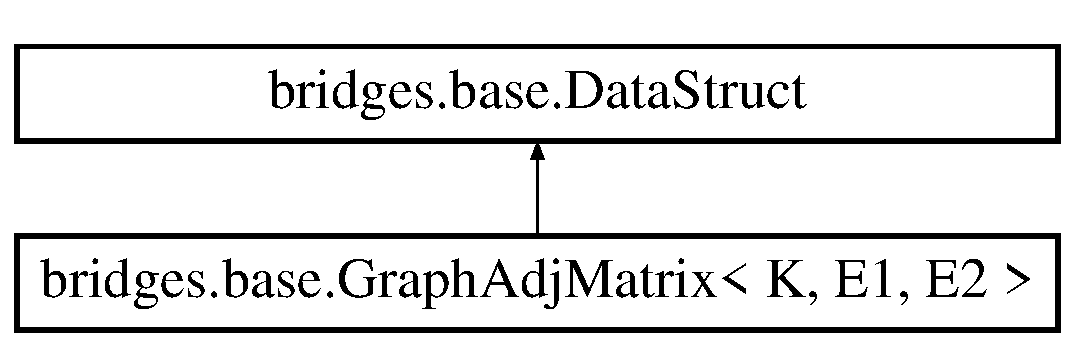
\includegraphics[height=2.000000cm]{classbridges_1_1base_1_1_graph_adj_matrix}
\end{center}
\end{figure}


\subsection{Detailed Description}
The \hyperlink{classbridges_1_1base_1_1_graph_adj_matrix}{Graph\+Adj\+Matrix} class can be used to represent adjacency matrix based graphs in B\+R\+I\+D\+G\+ES. 

The \hyperlink{classbridges_1_1base_1_1_graph_adj_matrix}{Graph\+Adj\+Matrix} class can be used to represent adjacency matrix based graphs in B\+R\+I\+D\+G\+ES; it takes 2 generic parameters\+: (1) K, which is an orderable key value used in accessing vertices (in constant time) using a hashmap. This permits data sets that need to be accessed by keys that are strings, and (2) E, an application defined type, and used in the \hyperlink{classbridges_1_1base_1_1_edge}{Edge} representation. The class is simply a wrapper around the Java Hashmap class and, thus, derives all its operations from it. B\+R\+I\+D\+G\+ES provides methods to visualize the graph and its contents.

The vertices of the graph are held in a Java hashmap, for near constant time access; this lets us use strings or integral ids for vertices. The edges are accessed by a second hashmap from each vertex, again assuring near constant access time. Each edge contains the terminating vertex id and weight, as defined by the \hyperlink{classbridges_1_1base_1_1_edge}{Edge} class structure.

Convenience methods are provided to add vertices and edges to the graph. Edges are retrieved by using the dual hashmap, given the vertex ids of the edge. Methods to access the element and link visualizer are now provided, indexed vertex ids, making it easier to set visual attributes to graph nodes and links.

\begin{DoxySeeAlso}{See also}
Example tutorial at \href{http://bridgesuncc.github.io/tutorials/Graph_AM.html}{\tt http\+://bridgesuncc.\+github.\+io/tutorials/\+Graph\+\_\+\+A\+M.\+html}
\end{DoxySeeAlso}
\begin{DoxyAuthor}{Author}
Kalpathi Subramanian, Mihai Mehedint
\end{DoxyAuthor}
\begin{DoxyDate}{Date}
7/12/15, 5/18/17, 4/23/18
\end{DoxyDate}

\begin{DoxyParams}{Parameters}
{\em K} & orderable key (string, int, etc) that is used to index into vertex \\
\hline
{\em E1} & vertex specific information, for graph vertices \\
\hline
{\em E2} & edge specific information, for graph vertices \\
\hline
\end{DoxyParams}
\subsection*{Public Member Functions}
\begin{DoxyCompactItemize}
\item 
\hyperlink{classbridges_1_1base_1_1_graph_adj_matrix_a8af4a2575890c3e68da7b39d800267bb}{Graph\+Adj\+Matrix} ()
\item 
String \hyperlink{classbridges_1_1base_1_1_graph_adj_matrix_a16ee088c4c53a9a5cdf3fbbad25cd1af}{get\+Data\+Struct\+Type} ()
\item 
void \hyperlink{classbridges_1_1base_1_1_graph_adj_matrix_a27b5ddb10a6615693460955b6bb3ee0c}{add\+Vertex} (K k, E1 e)
\item 
void \hyperlink{classbridges_1_1base_1_1_graph_adj_matrix_a477fbb5abbed6988e67b4b46b571e87c}{add\+Edge} (K src, K dest)
\item 
void \hyperlink{classbridges_1_1base_1_1_graph_adj_matrix_ad9b05b61e9592fa94045d7b59971b206}{add\+Edge} (K src, K dest, int weight)
\item 
void \hyperlink{classbridges_1_1base_1_1_graph_adj_matrix_a22eee632463a665e7016cf50916dfd83}{set\+Vertex\+Data} (K src, E1 vertex\+\_\+data)
\begin{DoxyCompactList}\small\item\em Sets data for a graph vertex. \end{DoxyCompactList}\item 
E1 \hyperlink{classbridges_1_1base_1_1_graph_adj_matrix_a36308a365d1c0f137ffb9a8e76a630f1}{get\+Vertex\+Data} (K src)
\item 
void \hyperlink{classbridges_1_1base_1_1_graph_adj_matrix_a72fe8bd594e3da28ba6e412de88576da}{set\+Edge\+Data} (K src, K dest, E2 data)
\item 
E2 \hyperlink{classbridges_1_1base_1_1_graph_adj_matrix_a3a3795c994ef9033ddb0b1d97029350b}{get\+Edge\+Data} (K src, K dest)
\item 
Hash\+Map$<$ K, \hyperlink{classbridges_1_1base_1_1_element}{Element}$<$ E1 $>$ $>$ \hyperlink{classbridges_1_1base_1_1_graph_adj_matrix_a6a000a302a1082bc2c55fbe8f511fce4}{get\+Vertices} ()
\item 
Hash\+Map$<$ K, Hash\+Map$<$ K, Integer $>$ $>$ \hyperlink{classbridges_1_1base_1_1_graph_adj_matrix_abe7f26cb9874744bc044df18b5d0eb84}{get\+Adjacency\+Matrix} ()
\item 
Hash\+Map$<$ K, Integer $>$ \hyperlink{classbridges_1_1base_1_1_graph_adj_matrix_a43f830cfe126f2be351f6d8c2fccc569}{get\+Adjacency\+Matrix} (K key)
\item 
\hyperlink{classbridges_1_1base_1_1_link_visualizer}{Link\+Visualizer} \hyperlink{classbridges_1_1base_1_1_graph_adj_matrix_a434454a6c8a1fac612392dcf1951dc9d}{get\+Link\+Visualizer} (K src, K dest)  throws Exception 
\item 
\hyperlink{classbridges_1_1base_1_1_element_visualizer}{Element\+Visualizer} \hyperlink{classbridges_1_1base_1_1_graph_adj_matrix_a4358ebee834c69796479a4ee6dfd96b3}{get\+Visualizer} (K vertex)  throws Exception 
\item 
String \hyperlink{classbridges_1_1base_1_1_graph_adj_matrix_ab0786f047bd0c8c47f19d632a1f03eaa}{get\+Data\+Structure\+Representation} ()
\end{DoxyCompactItemize}
\subsection*{Additional Inherited Members}


\subsection{Constructor \& Destructor Documentation}
\mbox{\Hypertarget{classbridges_1_1base_1_1_graph_adj_matrix_a8af4a2575890c3e68da7b39d800267bb}\label{classbridges_1_1base_1_1_graph_adj_matrix_a8af4a2575890c3e68da7b39d800267bb}} 
\index{bridges\+::base\+::\+Graph\+Adj\+Matrix@{bridges\+::base\+::\+Graph\+Adj\+Matrix}!Graph\+Adj\+Matrix@{Graph\+Adj\+Matrix}}
\index{Graph\+Adj\+Matrix@{Graph\+Adj\+Matrix}!bridges\+::base\+::\+Graph\+Adj\+Matrix@{bridges\+::base\+::\+Graph\+Adj\+Matrix}}
\subsubsection{\texorpdfstring{Graph\+Adj\+Matrix()}{GraphAdjMatrix()}}
{\footnotesize\ttfamily \hyperlink{classbridges_1_1base_1_1_graph_adj_matrix}{bridges.\+base.\+Graph\+Adj\+Matrix}$<$ K, E1, E2 $>$.\hyperlink{classbridges_1_1base_1_1_graph_adj_matrix}{Graph\+Adj\+Matrix} (\begin{DoxyParamCaption}{ }\end{DoxyParamCaption})}

Constructor 

\subsection{Member Function Documentation}
\mbox{\Hypertarget{classbridges_1_1base_1_1_graph_adj_matrix_a477fbb5abbed6988e67b4b46b571e87c}\label{classbridges_1_1base_1_1_graph_adj_matrix_a477fbb5abbed6988e67b4b46b571e87c}} 
\index{bridges\+::base\+::\+Graph\+Adj\+Matrix@{bridges\+::base\+::\+Graph\+Adj\+Matrix}!add\+Edge@{add\+Edge}}
\index{add\+Edge@{add\+Edge}!bridges\+::base\+::\+Graph\+Adj\+Matrix@{bridges\+::base\+::\+Graph\+Adj\+Matrix}}
\subsubsection{\texorpdfstring{add\+Edge()}{addEdge()}\hspace{0.1cm}{\footnotesize\ttfamily [1/2]}}
{\footnotesize\ttfamily void \hyperlink{classbridges_1_1base_1_1_graph_adj_matrix}{bridges.\+base.\+Graph\+Adj\+Matrix}$<$ K, E1, E2 $>$.add\+Edge (\begin{DoxyParamCaption}\item[{K}]{src,  }\item[{K}]{dest }\end{DoxyParamCaption})}

Adds a new edge to the graph, adds it to the index corresponding to the source, destination vertex ids; this version of the method assumes an edge weight of 1 (unweighted graph); user is responsible for checking if the vertices already exist, else an exception is thrown.


\begin{DoxyParams}{Parameters}
{\em src} & -\/ source vertex of edge \\
\hline
{\em dest} & -\/ destination vertex of edge \\
\hline
\end{DoxyParams}
\mbox{\Hypertarget{classbridges_1_1base_1_1_graph_adj_matrix_ad9b05b61e9592fa94045d7b59971b206}\label{classbridges_1_1base_1_1_graph_adj_matrix_ad9b05b61e9592fa94045d7b59971b206}} 
\index{bridges\+::base\+::\+Graph\+Adj\+Matrix@{bridges\+::base\+::\+Graph\+Adj\+Matrix}!add\+Edge@{add\+Edge}}
\index{add\+Edge@{add\+Edge}!bridges\+::base\+::\+Graph\+Adj\+Matrix@{bridges\+::base\+::\+Graph\+Adj\+Matrix}}
\subsubsection{\texorpdfstring{add\+Edge()}{addEdge()}\hspace{0.1cm}{\footnotesize\ttfamily [2/2]}}
{\footnotesize\ttfamily void \hyperlink{classbridges_1_1base_1_1_graph_adj_matrix}{bridges.\+base.\+Graph\+Adj\+Matrix}$<$ K, E1, E2 $>$.add\+Edge (\begin{DoxyParamCaption}\item[{K}]{src,  }\item[{K}]{dest,  }\item[{int}]{weight }\end{DoxyParamCaption})}

Adds a new edge of weight \textquotesingle{}weight\textquotesingle{} to the graph, adds it to the index corresponding to the source, destination vertex ids; user is responsible for checking if the vertices already exist, else an exception is thrown.


\begin{DoxyParams}{Parameters}
{\em src} & -\/ source vertex of edge \\
\hline
{\em dest} & -\/ destination vertex of edge \\
\hline
{\em weight} & -\/ edge weight \\
\hline
\end{DoxyParams}
\mbox{\Hypertarget{classbridges_1_1base_1_1_graph_adj_matrix_a27b5ddb10a6615693460955b6bb3ee0c}\label{classbridges_1_1base_1_1_graph_adj_matrix_a27b5ddb10a6615693460955b6bb3ee0c}} 
\index{bridges\+::base\+::\+Graph\+Adj\+Matrix@{bridges\+::base\+::\+Graph\+Adj\+Matrix}!add\+Vertex@{add\+Vertex}}
\index{add\+Vertex@{add\+Vertex}!bridges\+::base\+::\+Graph\+Adj\+Matrix@{bridges\+::base\+::\+Graph\+Adj\+Matrix}}
\subsubsection{\texorpdfstring{add\+Vertex()}{addVertex()}}
{\footnotesize\ttfamily void \hyperlink{classbridges_1_1base_1_1_graph_adj_matrix}{bridges.\+base.\+Graph\+Adj\+Matrix}$<$ K, E1, E2 $>$.add\+Vertex (\begin{DoxyParamCaption}\item[{K}]{k,  }\item[{E1}]{e }\end{DoxyParamCaption})}

Adds a new vertex to the graph, initializes the adjacency list; user is responsible for checking if the vertex already exists. This method will replace the value for this key


\begin{DoxyParams}{Parameters}
{\em k} & -\/ vertex key value \\
\hline
{\em e} & -\/ user specified data, part of the vertex data \\
\hline
\end{DoxyParams}
\mbox{\Hypertarget{classbridges_1_1base_1_1_graph_adj_matrix_abe7f26cb9874744bc044df18b5d0eb84}\label{classbridges_1_1base_1_1_graph_adj_matrix_abe7f26cb9874744bc044df18b5d0eb84}} 
\index{bridges\+::base\+::\+Graph\+Adj\+Matrix@{bridges\+::base\+::\+Graph\+Adj\+Matrix}!get\+Adjacency\+Matrix@{get\+Adjacency\+Matrix}}
\index{get\+Adjacency\+Matrix@{get\+Adjacency\+Matrix}!bridges\+::base\+::\+Graph\+Adj\+Matrix@{bridges\+::base\+::\+Graph\+Adj\+Matrix}}
\subsubsection{\texorpdfstring{get\+Adjacency\+Matrix()}{getAdjacencyMatrix()}\hspace{0.1cm}{\footnotesize\ttfamily [1/2]}}
{\footnotesize\ttfamily Hash\+Map$<$K, Hash\+Map$<$K, Integer$>$ $>$ \hyperlink{classbridges_1_1base_1_1_graph_adj_matrix}{bridges.\+base.\+Graph\+Adj\+Matrix}$<$ K, E1, E2 $>$.get\+Adjacency\+Matrix (\begin{DoxyParamCaption}{ }\end{DoxyParamCaption})}

Gets the adjacency matrix

\begin{DoxyReturn}{Returns}
-\/ the graph\textquotesingle{}s adjacency matrix 
\end{DoxyReturn}
\mbox{\Hypertarget{classbridges_1_1base_1_1_graph_adj_matrix_a43f830cfe126f2be351f6d8c2fccc569}\label{classbridges_1_1base_1_1_graph_adj_matrix_a43f830cfe126f2be351f6d8c2fccc569}} 
\index{bridges\+::base\+::\+Graph\+Adj\+Matrix@{bridges\+::base\+::\+Graph\+Adj\+Matrix}!get\+Adjacency\+Matrix@{get\+Adjacency\+Matrix}}
\index{get\+Adjacency\+Matrix@{get\+Adjacency\+Matrix}!bridges\+::base\+::\+Graph\+Adj\+Matrix@{bridges\+::base\+::\+Graph\+Adj\+Matrix}}
\subsubsection{\texorpdfstring{get\+Adjacency\+Matrix()}{getAdjacencyMatrix()}\hspace{0.1cm}{\footnotesize\ttfamily [2/2]}}
{\footnotesize\ttfamily Hash\+Map$<$K, Integer$>$ \hyperlink{classbridges_1_1base_1_1_graph_adj_matrix}{bridges.\+base.\+Graph\+Adj\+Matrix}$<$ K, E1, E2 $>$.get\+Adjacency\+Matrix (\begin{DoxyParamCaption}\item[{K}]{key }\end{DoxyParamCaption})}

Gets the row of the adjacency matrix corresponding to the key


\begin{DoxyParams}{Parameters}
{\em key} & key value \\
\hline
\end{DoxyParams}
\begin{DoxyReturn}{Returns}
-\/ the graph\textquotesingle{}s adjacency matrix 
\end{DoxyReturn}
\mbox{\Hypertarget{classbridges_1_1base_1_1_graph_adj_matrix_a16ee088c4c53a9a5cdf3fbbad25cd1af}\label{classbridges_1_1base_1_1_graph_adj_matrix_a16ee088c4c53a9a5cdf3fbbad25cd1af}} 
\index{bridges\+::base\+::\+Graph\+Adj\+Matrix@{bridges\+::base\+::\+Graph\+Adj\+Matrix}!get\+Data\+Struct\+Type@{get\+Data\+Struct\+Type}}
\index{get\+Data\+Struct\+Type@{get\+Data\+Struct\+Type}!bridges\+::base\+::\+Graph\+Adj\+Matrix@{bridges\+::base\+::\+Graph\+Adj\+Matrix}}
\subsubsection{\texorpdfstring{get\+Data\+Struct\+Type()}{getDataStructType()}}
{\footnotesize\ttfamily String \hyperlink{classbridges_1_1base_1_1_graph_adj_matrix}{bridges.\+base.\+Graph\+Adj\+Matrix}$<$ K, E1, E2 $>$.get\+Data\+Struct\+Type (\begin{DoxyParamCaption}{ }\end{DoxyParamCaption})}

This method gets the data structure type

\begin{DoxyReturn}{Returns}
The date structure type as a string 
\end{DoxyReturn}
\mbox{\Hypertarget{classbridges_1_1base_1_1_graph_adj_matrix_ab0786f047bd0c8c47f19d632a1f03eaa}\label{classbridges_1_1base_1_1_graph_adj_matrix_ab0786f047bd0c8c47f19d632a1f03eaa}} 
\index{bridges\+::base\+::\+Graph\+Adj\+Matrix@{bridges\+::base\+::\+Graph\+Adj\+Matrix}!get\+Data\+Structure\+Representation@{get\+Data\+Structure\+Representation}}
\index{get\+Data\+Structure\+Representation@{get\+Data\+Structure\+Representation}!bridges\+::base\+::\+Graph\+Adj\+Matrix@{bridges\+::base\+::\+Graph\+Adj\+Matrix}}
\subsubsection{\texorpdfstring{get\+Data\+Structure\+Representation()}{getDataStructureRepresentation()}}
{\footnotesize\ttfamily String \hyperlink{classbridges_1_1base_1_1_graph_adj_matrix}{bridges.\+base.\+Graph\+Adj\+Matrix}$<$ K, E1, E2 $>$.get\+Data\+Structure\+Representation (\begin{DoxyParamCaption}{ }\end{DoxyParamCaption})}

\mbox{\Hypertarget{classbridges_1_1base_1_1_graph_adj_matrix_a3a3795c994ef9033ddb0b1d97029350b}\label{classbridges_1_1base_1_1_graph_adj_matrix_a3a3795c994ef9033ddb0b1d97029350b}} 
\index{bridges\+::base\+::\+Graph\+Adj\+Matrix@{bridges\+::base\+::\+Graph\+Adj\+Matrix}!get\+Edge\+Data@{get\+Edge\+Data}}
\index{get\+Edge\+Data@{get\+Edge\+Data}!bridges\+::base\+::\+Graph\+Adj\+Matrix@{bridges\+::base\+::\+Graph\+Adj\+Matrix}}
\subsubsection{\texorpdfstring{get\+Edge\+Data()}{getEdgeData()}}
{\footnotesize\ttfamily E2 \hyperlink{classbridges_1_1base_1_1_graph_adj_matrix}{bridges.\+base.\+Graph\+Adj\+Matrix}$<$ K, E1, E2 $>$.get\+Edge\+Data (\begin{DoxyParamCaption}\item[{K}]{src,  }\item[{K}]{dest }\end{DoxyParamCaption})}

Gets data for an edge


\begin{DoxyParams}{Parameters}
{\em src} & -\/ source vertex of edge \\
\hline
{\em dest} & -\/ destination vertex of edge \\
\hline
\end{DoxyParams}
\mbox{\Hypertarget{classbridges_1_1base_1_1_graph_adj_matrix_a434454a6c8a1fac612392dcf1951dc9d}\label{classbridges_1_1base_1_1_graph_adj_matrix_a434454a6c8a1fac612392dcf1951dc9d}} 
\index{bridges\+::base\+::\+Graph\+Adj\+Matrix@{bridges\+::base\+::\+Graph\+Adj\+Matrix}!get\+Link\+Visualizer@{get\+Link\+Visualizer}}
\index{get\+Link\+Visualizer@{get\+Link\+Visualizer}!bridges\+::base\+::\+Graph\+Adj\+Matrix@{bridges\+::base\+::\+Graph\+Adj\+Matrix}}
\subsubsection{\texorpdfstring{get\+Link\+Visualizer()}{getLinkVisualizer()}}
{\footnotesize\ttfamily \hyperlink{classbridges_1_1base_1_1_link_visualizer}{Link\+Visualizer} \hyperlink{classbridges_1_1base_1_1_graph_adj_matrix}{bridges.\+base.\+Graph\+Adj\+Matrix}$<$ K, E1, E2 $>$.get\+Link\+Visualizer (\begin{DoxyParamCaption}\item[{K}]{src,  }\item[{K}]{dest }\end{DoxyParamCaption}) throws Exception}

This is a convenience method to simplify access to the link visualizer; the method assumes the vertex names point to existing vertices, else an exception is thrown \mbox{\Hypertarget{classbridges_1_1base_1_1_graph_adj_matrix_a36308a365d1c0f137ffb9a8e76a630f1}\label{classbridges_1_1base_1_1_graph_adj_matrix_a36308a365d1c0f137ffb9a8e76a630f1}} 
\index{bridges\+::base\+::\+Graph\+Adj\+Matrix@{bridges\+::base\+::\+Graph\+Adj\+Matrix}!get\+Vertex\+Data@{get\+Vertex\+Data}}
\index{get\+Vertex\+Data@{get\+Vertex\+Data}!bridges\+::base\+::\+Graph\+Adj\+Matrix@{bridges\+::base\+::\+Graph\+Adj\+Matrix}}
\subsubsection{\texorpdfstring{get\+Vertex\+Data()}{getVertexData()}}
{\footnotesize\ttfamily E1 \hyperlink{classbridges_1_1base_1_1_graph_adj_matrix}{bridges.\+base.\+Graph\+Adj\+Matrix}$<$ K, E1, E2 $>$.get\+Vertex\+Data (\begin{DoxyParamCaption}\item[{K}]{src }\end{DoxyParamCaption})}

Gets data for a vertex


\begin{DoxyParams}{Parameters}
{\em src} & source vertex of edge \\
\hline
\end{DoxyParams}
\mbox{\Hypertarget{classbridges_1_1base_1_1_graph_adj_matrix_a6a000a302a1082bc2c55fbe8f511fce4}\label{classbridges_1_1base_1_1_graph_adj_matrix_a6a000a302a1082bc2c55fbe8f511fce4}} 
\index{bridges\+::base\+::\+Graph\+Adj\+Matrix@{bridges\+::base\+::\+Graph\+Adj\+Matrix}!get\+Vertices@{get\+Vertices}}
\index{get\+Vertices@{get\+Vertices}!bridges\+::base\+::\+Graph\+Adj\+Matrix@{bridges\+::base\+::\+Graph\+Adj\+Matrix}}
\subsubsection{\texorpdfstring{get\+Vertices()}{getVertices()}}
{\footnotesize\ttfamily Hash\+Map$<$K, \hyperlink{classbridges_1_1base_1_1_element}{Element}$<$E1$>$ $>$ \hyperlink{classbridges_1_1base_1_1_graph_adj_matrix}{bridges.\+base.\+Graph\+Adj\+Matrix}$<$ K, E1, E2 $>$.get\+Vertices (\begin{DoxyParamCaption}{ }\end{DoxyParamCaption})}

This method returns the graph nodes 

return -- vertices held in an unordered map \mbox{\Hypertarget{classbridges_1_1base_1_1_graph_adj_matrix_a4358ebee834c69796479a4ee6dfd96b3}\label{classbridges_1_1base_1_1_graph_adj_matrix_a4358ebee834c69796479a4ee6dfd96b3}} 
\index{bridges\+::base\+::\+Graph\+Adj\+Matrix@{bridges\+::base\+::\+Graph\+Adj\+Matrix}!get\+Visualizer@{get\+Visualizer}}
\index{get\+Visualizer@{get\+Visualizer}!bridges\+::base\+::\+Graph\+Adj\+Matrix@{bridges\+::base\+::\+Graph\+Adj\+Matrix}}
\subsubsection{\texorpdfstring{get\+Visualizer()}{getVisualizer()}}
{\footnotesize\ttfamily \hyperlink{classbridges_1_1base_1_1_element_visualizer}{Element\+Visualizer} \hyperlink{classbridges_1_1base_1_1_graph_adj_matrix}{bridges.\+base.\+Graph\+Adj\+Matrix}$<$ K, E1, E2 $>$.get\+Visualizer (\begin{DoxyParamCaption}\item[{K}]{vertex }\end{DoxyParamCaption}) throws Exception}

This is a convenience method to simplify access to the element visualizer; the method assumes the vertex name points to an existing vertice, else an exception is thrown \mbox{\Hypertarget{classbridges_1_1base_1_1_graph_adj_matrix_a72fe8bd594e3da28ba6e412de88576da}\label{classbridges_1_1base_1_1_graph_adj_matrix_a72fe8bd594e3da28ba6e412de88576da}} 
\index{bridges\+::base\+::\+Graph\+Adj\+Matrix@{bridges\+::base\+::\+Graph\+Adj\+Matrix}!set\+Edge\+Data@{set\+Edge\+Data}}
\index{set\+Edge\+Data@{set\+Edge\+Data}!bridges\+::base\+::\+Graph\+Adj\+Matrix@{bridges\+::base\+::\+Graph\+Adj\+Matrix}}
\subsubsection{\texorpdfstring{set\+Edge\+Data()}{setEdgeData()}}
{\footnotesize\ttfamily void \hyperlink{classbridges_1_1base_1_1_graph_adj_matrix}{bridges.\+base.\+Graph\+Adj\+Matrix}$<$ K, E1, E2 $>$.set\+Edge\+Data (\begin{DoxyParamCaption}\item[{K}]{src,  }\item[{K}]{dest,  }\item[{E2}]{data }\end{DoxyParamCaption})}

Sets data for an edge


\begin{DoxyParams}{Parameters}
{\em src} & -\/ source vertex of edge \\
\hline
{\em dest} & -\/ destination vertex of edge \\
\hline
{\em data} & -\/ edge data \\
\hline
\end{DoxyParams}
\mbox{\Hypertarget{classbridges_1_1base_1_1_graph_adj_matrix_a22eee632463a665e7016cf50916dfd83}\label{classbridges_1_1base_1_1_graph_adj_matrix_a22eee632463a665e7016cf50916dfd83}} 
\index{bridges\+::base\+::\+Graph\+Adj\+Matrix@{bridges\+::base\+::\+Graph\+Adj\+Matrix}!set\+Vertex\+Data@{set\+Vertex\+Data}}
\index{set\+Vertex\+Data@{set\+Vertex\+Data}!bridges\+::base\+::\+Graph\+Adj\+Matrix@{bridges\+::base\+::\+Graph\+Adj\+Matrix}}
\subsubsection{\texorpdfstring{set\+Vertex\+Data()}{setVertexData()}}
{\footnotesize\ttfamily void \hyperlink{classbridges_1_1base_1_1_graph_adj_matrix}{bridges.\+base.\+Graph\+Adj\+Matrix}$<$ K, E1, E2 $>$.set\+Vertex\+Data (\begin{DoxyParamCaption}\item[{K}]{src,  }\item[{E1}]{vertex\+\_\+data }\end{DoxyParamCaption})}



Sets data for a graph vertex. 


\begin{DoxyParams}{Parameters}
{\em src} & source vertex of edge \\
\hline
{\em vertex\+\_\+data} & vertex data \\
\hline
\end{DoxyParams}


The documentation for this class was generated from the following file\+:\begin{DoxyCompactItemize}
\item 
/home/erik/work/bridges/bridges-\/java/src/main/java/bridges/base/\hyperlink{_graph_adj_matrix_8java}{Graph\+Adj\+Matrix.\+java}\end{DoxyCompactItemize}

\hypertarget{classbridges_1_1base_1_1_graph_adj_matrix_simple}{}\section{bridges.\+base.\+Graph\+Adj\+Matrix\+Simple$<$ K $>$ Class Template Reference}
\label{classbridges_1_1base_1_1_graph_adj_matrix_simple}\index{bridges.\+base.\+Graph\+Adj\+Matrix\+Simple$<$ K $>$@{bridges.\+base.\+Graph\+Adj\+Matrix\+Simple$<$ K $>$}}


The \mbox{\hyperlink{classbridges_1_1base_1_1_graph_adj_matrix_simple}{Graph\+Adj\+Matrix\+Simple}} class is a simplification of the \mbox{\hyperlink{classbridges_1_1base_1_1_graph_adj_matrix}{Graph\+Adj\+Matrix}} class; this class is useful in applications where vertex and edge specific information is not used; this class is thus a specialization of \mbox{\hyperlink{classbridges_1_1base_1_1_graph_adj_list}{Graph\+Adj\+List}} with only a single generic parameter that specifies the key type.  


Inheritance diagram for bridges.\+base.\+Graph\+Adj\+Matrix\+Simple$<$ K $>$\+:\begin{figure}[H]
\begin{center}
\leavevmode
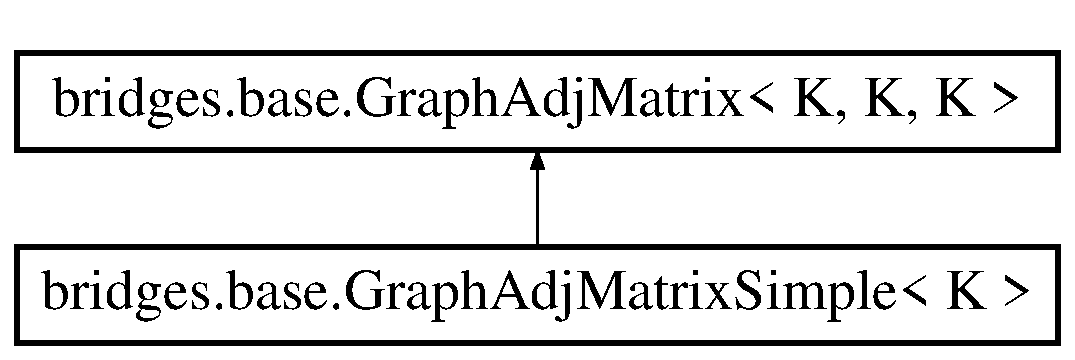
\includegraphics[height=2.000000cm]{classbridges_1_1base_1_1_graph_adj_matrix_simple}
\end{center}
\end{figure}
\subsection*{Additional Inherited Members}


\subsection{Detailed Description}
The \mbox{\hyperlink{classbridges_1_1base_1_1_graph_adj_matrix_simple}{Graph\+Adj\+Matrix\+Simple}} class is a simplification of the \mbox{\hyperlink{classbridges_1_1base_1_1_graph_adj_matrix}{Graph\+Adj\+Matrix}} class; this class is useful in applications where vertex and edge specific information is not used; this class is thus a specialization of \mbox{\hyperlink{classbridges_1_1base_1_1_graph_adj_list}{Graph\+Adj\+List}} with only a single generic parameter that specifies the key type. 

The \mbox{\hyperlink{classbridges_1_1base_1_1_graph_adj_matrix_simple}{Graph\+Adj\+Matrix\+Simple}} class can be used to represent adjacency list based ~\newline
graphs in B\+R\+I\+D\+G\+ES; it takes 1 generic parameter\+: K, which is an orderable key value used in accessing vertices and edges (in constant time) using hashmaps. This permits data sets that need to be accessed by keys that are strings. Vertex and edge specific information can still be represented, but they will be restricted to be of type K.

The class is simply a wrapper around the Java Hashmap class and, thus, derives all its operations from it. B\+R\+I\+D\+G\+ES provides methods to visualize the graph and its contents.

The vertices of the graph are held in a Java hashmap of hashmaps(2\+D hashmap), for near constant time access; this lets us use strings or integral ids for vertices. \mbox{\hyperlink{classbridges_1_1base_1_1_edge}{Edge}} information is also held in a hashmap with accessor methods.

Convenience methods are provided to add vertices and edges to the graph as well as retrieve the adjacency list of a vertex, given its id. Methods to access and set visual attributes are also provided, indexed by the vertex ids.

\begin{DoxyAuthor}{Author}
Kalpathi Subramanian
\end{DoxyAuthor}
\begin{DoxyDate}{Date}
4/24/18
\end{DoxyDate}

\begin{DoxyParams}{Parameters}
{\em $<$\+K$>$} & orderable key (string, int, etc) that is used to index into vertex\\
\hline
\end{DoxyParams}
\begin{DoxySeeAlso}{See also}
Example tutorial at 
\end{DoxySeeAlso}
\href{http://bridgesuncc.github.io/Hello_World_Tutorials/Graph.html}{\tt http\+://bridgesuncc.\+github.\+io/\+Hello\+\_\+\+World\+\_\+\+Tutorials/\+Graph.\+html} 

The documentation for this class was generated from the following file\+:\begin{DoxyCompactItemize}
\item 
/\+Users/kalpathi/gr/bridges/client/java/bridges-\/17/src/main/java/edu/uncc/cs/bridges\+\_\+v21/base/\mbox{\hyperlink{_graph_adj_matrix_simple_8java}{Graph\+Adj\+Matrix\+Simple.\+java}}\end{DoxyCompactItemize}

\hypertarget{classbridges_1_1base_1_1_grid}{}\section{bridges.\+base.\+Grid$<$ E $>$ Class Template Reference}
\label{classbridges_1_1base_1_1_grid}\index{bridges.\+base.\+Grid$<$ E $>$@{bridges.\+base.\+Grid$<$ E $>$}}
Inheritance diagram for bridges.\+base.\+Grid$<$ E $>$\+:\begin{figure}[H]
\begin{center}
\leavevmode
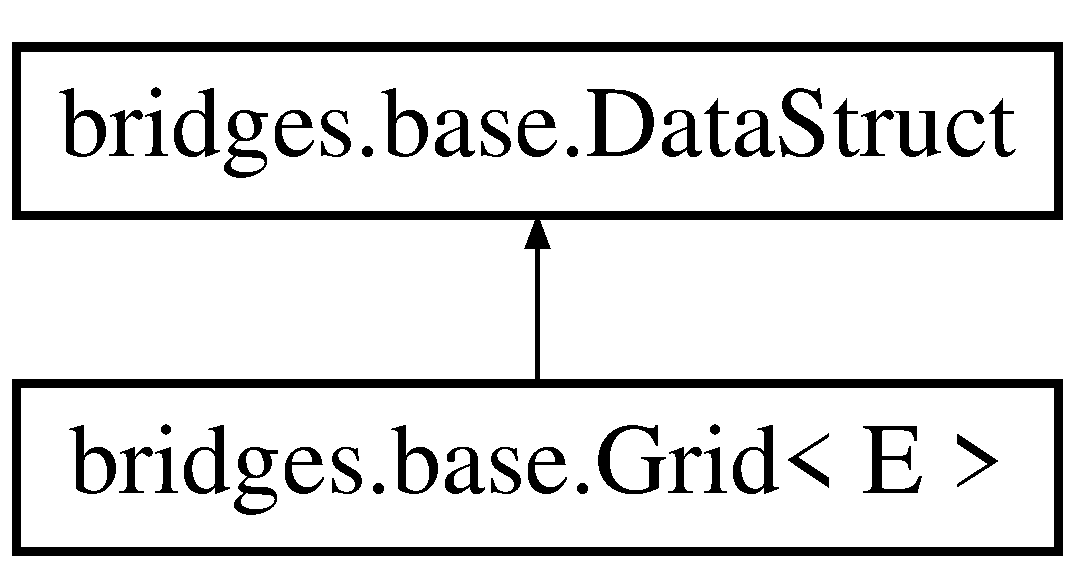
\includegraphics[height=2.000000cm]{classbridges_1_1base_1_1_grid}
\end{center}
\end{figure}


\subsection{Detailed Description}
This is a class in B\+R\+I\+D\+G\+ES for representing an (m x n) grid. 

\begin{DoxyAuthor}{Author}
David Burlinson 
\end{DoxyAuthor}
\begin{DoxyDate}{Date}
5/14/18, 7/14/19 
\end{DoxyDate}
\subsection*{Public Member Functions}
\begin{DoxyCompactItemize}
\item 
String \mbox{\hyperlink{classbridges_1_1base_1_1_grid_a81f268dd27c292ff2af9358039d4ebe6}{get\+Data\+Struct\+Type}} ()
\item 
\mbox{\hyperlink{classbridges_1_1base_1_1_grid_aa621ffc958db8341f7ce37ed78944d51}{Grid}} ()
\item 
\mbox{\hyperlink{classbridges_1_1base_1_1_grid_a9818d4959813f1292c6a234bc6f6aa9e}{Grid}} (int size)
\item 
\mbox{\hyperlink{classbridges_1_1base_1_1_grid_a43a699bd7ae2c6c986f978c515ff97d8}{Grid}} (int rows, int cols)
\item 
\mbox{\hyperlink{classbridges_1_1base_1_1_grid_ab9975b28d8dda7f3fbe0e35a7a026772}{Grid}} (int\mbox{[}$\,$\mbox{]} size)
\item 
int \mbox{[}$\,$\mbox{]} \mbox{\hyperlink{classbridges_1_1base_1_1_grid_aee8a5b66095d65ff067a4e76f2611b0e}{get\+Dimensions}} ()
\item 
E \mbox{\hyperlink{classbridges_1_1base_1_1_grid_a698579bb5b7166f76a18a1b04916e090}{get}} (Integer row, Integer col)
\item 
void \mbox{\hyperlink{classbridges_1_1base_1_1_grid_ab79ceb737423bb28ea2348e61a625a17}{set}} (Integer row, Integer col, E val)
\item 
String \mbox{\hyperlink{classbridges_1_1base_1_1_grid_a9a7faf2bbabae8d2f2babe9e29deb2c8}{get\+Data\+Structure\+Representation}} ()
\end{DoxyCompactItemize}
\subsection*{Protected Attributes}
\begin{DoxyCompactItemize}
\item 
Array\+List$<$ Array\+List$<$ E $>$ $>$ \mbox{\hyperlink{classbridges_1_1base_1_1_grid_ad1f3f6968d58188425bd992c05c655a6}{grid}}
\item 
int \mbox{[}$\,$\mbox{]} \mbox{\hyperlink{classbridges_1_1base_1_1_grid_a54a66479f78022570253d771206a0420}{grid\+Size}}
\end{DoxyCompactItemize}
\subsection*{Static Protected Attributes}
\begin{DoxyCompactItemize}
\item 
static final int \mbox{[}$\,$\mbox{]} \mbox{\hyperlink{classbridges_1_1base_1_1_grid_a45c2786d2af83624202192857a27724f}{default\+Grid\+Size}} = \{10, 10\}
\item 
static int \mbox{[}$\,$\mbox{]} \mbox{\hyperlink{classbridges_1_1base_1_1_grid_a803fd4c070a22863c82581f0bb258c1c}{max\+Grid\+Size}} = \{1080, 1920\}
\end{DoxyCompactItemize}


\subsection{Constructor \& Destructor Documentation}
\mbox{\Hypertarget{classbridges_1_1base_1_1_grid_aa621ffc958db8341f7ce37ed78944d51}\label{classbridges_1_1base_1_1_grid_aa621ffc958db8341f7ce37ed78944d51}} 
\index{bridges\+::base\+::\+Grid@{bridges\+::base\+::\+Grid}!Grid@{Grid}}
\index{Grid@{Grid}!bridges\+::base\+::\+Grid@{bridges\+::base\+::\+Grid}}
\subsubsection{\texorpdfstring{Grid()}{Grid()}\hspace{0.1cm}{\footnotesize\ttfamily [1/4]}}
{\footnotesize\ttfamily \mbox{\hyperlink{classbridges_1_1base_1_1_grid}{bridges.\+base.\+Grid}}$<$ E $>$.\mbox{\hyperlink{classbridges_1_1base_1_1_grid}{Grid}} (\begin{DoxyParamCaption}{ }\end{DoxyParamCaption})}

Construct a grid with default sizes \mbox{\Hypertarget{classbridges_1_1base_1_1_grid_a9818d4959813f1292c6a234bc6f6aa9e}\label{classbridges_1_1base_1_1_grid_a9818d4959813f1292c6a234bc6f6aa9e}} 
\index{bridges\+::base\+::\+Grid@{bridges\+::base\+::\+Grid}!Grid@{Grid}}
\index{Grid@{Grid}!bridges\+::base\+::\+Grid@{bridges\+::base\+::\+Grid}}
\subsubsection{\texorpdfstring{Grid()}{Grid()}\hspace{0.1cm}{\footnotesize\ttfamily [2/4]}}
{\footnotesize\ttfamily \mbox{\hyperlink{classbridges_1_1base_1_1_grid}{bridges.\+base.\+Grid}}$<$ E $>$.\mbox{\hyperlink{classbridges_1_1base_1_1_grid}{Grid}} (\begin{DoxyParamCaption}\item[{int}]{size }\end{DoxyParamCaption})}

Construct a size x size grid \mbox{\Hypertarget{classbridges_1_1base_1_1_grid_a43a699bd7ae2c6c986f978c515ff97d8}\label{classbridges_1_1base_1_1_grid_a43a699bd7ae2c6c986f978c515ff97d8}} 
\index{bridges\+::base\+::\+Grid@{bridges\+::base\+::\+Grid}!Grid@{Grid}}
\index{Grid@{Grid}!bridges\+::base\+::\+Grid@{bridges\+::base\+::\+Grid}}
\subsubsection{\texorpdfstring{Grid()}{Grid()}\hspace{0.1cm}{\footnotesize\ttfamily [3/4]}}
{\footnotesize\ttfamily \mbox{\hyperlink{classbridges_1_1base_1_1_grid}{bridges.\+base.\+Grid}}$<$ E $>$.\mbox{\hyperlink{classbridges_1_1base_1_1_grid}{Grid}} (\begin{DoxyParamCaption}\item[{int}]{rows,  }\item[{int}]{cols }\end{DoxyParamCaption})}

Construct a rows x cols size grid


\begin{DoxyParams}{Parameters}
{\em rows} & number of rows in grid \\
\hline
{\em cols} & number of rows in grid \\
\hline
\end{DoxyParams}
\mbox{\Hypertarget{classbridges_1_1base_1_1_grid_ab9975b28d8dda7f3fbe0e35a7a026772}\label{classbridges_1_1base_1_1_grid_ab9975b28d8dda7f3fbe0e35a7a026772}} 
\index{bridges\+::base\+::\+Grid@{bridges\+::base\+::\+Grid}!Grid@{Grid}}
\index{Grid@{Grid}!bridges\+::base\+::\+Grid@{bridges\+::base\+::\+Grid}}
\subsubsection{\texorpdfstring{Grid()}{Grid()}\hspace{0.1cm}{\footnotesize\ttfamily [4/4]}}
{\footnotesize\ttfamily \mbox{\hyperlink{classbridges_1_1base_1_1_grid}{bridges.\+base.\+Grid}}$<$ E $>$.\mbox{\hyperlink{classbridges_1_1base_1_1_grid}{Grid}} (\begin{DoxyParamCaption}\item[{int \mbox{[}$\,$\mbox{]}}]{size }\end{DoxyParamCaption})}

Construct a size\mbox{[}0\mbox{]} by size\mbox{[}1\mbox{]} sized grid 
\begin{DoxyParams}{Parameters}
{\em size\mbox{[}$\,$\mbox{]}} & specifies rows and column sizes of the grid \\
\hline
\end{DoxyParams}


\subsection{Member Function Documentation}
\mbox{\Hypertarget{classbridges_1_1base_1_1_grid_a698579bb5b7166f76a18a1b04916e090}\label{classbridges_1_1base_1_1_grid_a698579bb5b7166f76a18a1b04916e090}} 
\index{bridges\+::base\+::\+Grid@{bridges\+::base\+::\+Grid}!get@{get}}
\index{get@{get}!bridges\+::base\+::\+Grid@{bridges\+::base\+::\+Grid}}
\subsubsection{\texorpdfstring{get()}{get()}}
{\footnotesize\ttfamily E \mbox{\hyperlink{classbridges_1_1base_1_1_grid}{bridges.\+base.\+Grid}}$<$ E $>$.get (\begin{DoxyParamCaption}\item[{Integer}]{row,  }\item[{Integer}]{col }\end{DoxyParamCaption})}

Get the (row, col) element in the grid 
\begin{DoxyParams}{Parameters}
{\em row} & row number \\
\hline
{\em col} & number \\
\hline
\end{DoxyParams}
\mbox{\Hypertarget{classbridges_1_1base_1_1_grid_a81f268dd27c292ff2af9358039d4ebe6}\label{classbridges_1_1base_1_1_grid_a81f268dd27c292ff2af9358039d4ebe6}} 
\index{bridges\+::base\+::\+Grid@{bridges\+::base\+::\+Grid}!get\+Data\+Struct\+Type@{get\+Data\+Struct\+Type}}
\index{get\+Data\+Struct\+Type@{get\+Data\+Struct\+Type}!bridges\+::base\+::\+Grid@{bridges\+::base\+::\+Grid}}
\subsubsection{\texorpdfstring{get\+Data\+Struct\+Type()}{getDataStructType()}}
{\footnotesize\ttfamily String \mbox{\hyperlink{classbridges_1_1base_1_1_grid}{bridges.\+base.\+Grid}}$<$ E $>$.get\+Data\+Struct\+Type (\begin{DoxyParamCaption}{ }\end{DoxyParamCaption})}

Get data structure name \begin{DoxyReturn}{Returns}
data type name 
\end{DoxyReturn}
\mbox{\Hypertarget{classbridges_1_1base_1_1_grid_a9a7faf2bbabae8d2f2babe9e29deb2c8}\label{classbridges_1_1base_1_1_grid_a9a7faf2bbabae8d2f2babe9e29deb2c8}} 
\index{bridges\+::base\+::\+Grid@{bridges\+::base\+::\+Grid}!get\+Data\+Structure\+Representation@{get\+Data\+Structure\+Representation}}
\index{get\+Data\+Structure\+Representation@{get\+Data\+Structure\+Representation}!bridges\+::base\+::\+Grid@{bridges\+::base\+::\+Grid}}
\subsubsection{\texorpdfstring{get\+Data\+Structure\+Representation()}{getDataStructureRepresentation()}}
{\footnotesize\ttfamily String \mbox{\hyperlink{classbridges_1_1base_1_1_grid}{bridges.\+base.\+Grid}}$<$ E $>$.get\+Data\+Structure\+Representation (\begin{DoxyParamCaption}{ }\end{DoxyParamCaption})}

Get data structure representation \mbox{\Hypertarget{classbridges_1_1base_1_1_grid_aee8a5b66095d65ff067a4e76f2611b0e}\label{classbridges_1_1base_1_1_grid_aee8a5b66095d65ff067a4e76f2611b0e}} 
\index{bridges\+::base\+::\+Grid@{bridges\+::base\+::\+Grid}!get\+Dimensions@{get\+Dimensions}}
\index{get\+Dimensions@{get\+Dimensions}!bridges\+::base\+::\+Grid@{bridges\+::base\+::\+Grid}}
\subsubsection{\texorpdfstring{get\+Dimensions()}{getDimensions()}}
{\footnotesize\ttfamily int \mbox{[}$\,$\mbox{]} \mbox{\hyperlink{classbridges_1_1base_1_1_grid}{bridges.\+base.\+Grid}}$<$ E $>$.get\+Dimensions (\begin{DoxyParamCaption}{ }\end{DoxyParamCaption})}

Get the grid dimensions

\begin{DoxyReturn}{Returns}
an array of two values (rows, cols) of the grid 
\end{DoxyReturn}
\mbox{\Hypertarget{classbridges_1_1base_1_1_grid_ab79ceb737423bb28ea2348e61a625a17}\label{classbridges_1_1base_1_1_grid_ab79ceb737423bb28ea2348e61a625a17}} 
\index{bridges\+::base\+::\+Grid@{bridges\+::base\+::\+Grid}!set@{set}}
\index{set@{set}!bridges\+::base\+::\+Grid@{bridges\+::base\+::\+Grid}}
\subsubsection{\texorpdfstring{set()}{set()}}
{\footnotesize\ttfamily void \mbox{\hyperlink{classbridges_1_1base_1_1_grid}{bridges.\+base.\+Grid}}$<$ E $>$.set (\begin{DoxyParamCaption}\item[{Integer}]{row,  }\item[{Integer}]{col,  }\item[{E}]{val }\end{DoxyParamCaption})}

Set the (row, col) element in the grid 
\begin{DoxyParams}{Parameters}
{\em row,col} & cell to change \\
\hline
{\em val} & the value to be set to \\
\hline
\end{DoxyParams}


\subsection{Member Data Documentation}
\mbox{\Hypertarget{classbridges_1_1base_1_1_grid_a45c2786d2af83624202192857a27724f}\label{classbridges_1_1base_1_1_grid_a45c2786d2af83624202192857a27724f}} 
\index{bridges\+::base\+::\+Grid@{bridges\+::base\+::\+Grid}!default\+Grid\+Size@{default\+Grid\+Size}}
\index{default\+Grid\+Size@{default\+Grid\+Size}!bridges\+::base\+::\+Grid@{bridges\+::base\+::\+Grid}}
\subsubsection{\texorpdfstring{default\+Grid\+Size}{defaultGridSize}}
{\footnotesize\ttfamily final int \mbox{[}$\,$\mbox{]} \mbox{\hyperlink{classbridges_1_1base_1_1_grid}{bridges.\+base.\+Grid}}$<$ E $>$.default\+Grid\+Size = \{10, 10\}\hspace{0.3cm}{\ttfamily [static]}, {\ttfamily [protected]}}

\mbox{\Hypertarget{classbridges_1_1base_1_1_grid_ad1f3f6968d58188425bd992c05c655a6}\label{classbridges_1_1base_1_1_grid_ad1f3f6968d58188425bd992c05c655a6}} 
\index{bridges\+::base\+::\+Grid@{bridges\+::base\+::\+Grid}!grid@{grid}}
\index{grid@{grid}!bridges\+::base\+::\+Grid@{bridges\+::base\+::\+Grid}}
\subsubsection{\texorpdfstring{grid}{grid}}
{\footnotesize\ttfamily Array\+List$<$Array\+List$<$E$>$ $>$ \mbox{\hyperlink{classbridges_1_1base_1_1_grid}{bridges.\+base.\+Grid}}$<$ E $>$.grid\hspace{0.3cm}{\ttfamily [protected]}}

\mbox{\Hypertarget{classbridges_1_1base_1_1_grid_a54a66479f78022570253d771206a0420}\label{classbridges_1_1base_1_1_grid_a54a66479f78022570253d771206a0420}} 
\index{bridges\+::base\+::\+Grid@{bridges\+::base\+::\+Grid}!grid\+Size@{grid\+Size}}
\index{grid\+Size@{grid\+Size}!bridges\+::base\+::\+Grid@{bridges\+::base\+::\+Grid}}
\subsubsection{\texorpdfstring{grid\+Size}{gridSize}}
{\footnotesize\ttfamily int \mbox{[}$\,$\mbox{]} \mbox{\hyperlink{classbridges_1_1base_1_1_grid}{bridges.\+base.\+Grid}}$<$ E $>$.grid\+Size\hspace{0.3cm}{\ttfamily [protected]}}

\mbox{\Hypertarget{classbridges_1_1base_1_1_grid_a803fd4c070a22863c82581f0bb258c1c}\label{classbridges_1_1base_1_1_grid_a803fd4c070a22863c82581f0bb258c1c}} 
\index{bridges\+::base\+::\+Grid@{bridges\+::base\+::\+Grid}!max\+Grid\+Size@{max\+Grid\+Size}}
\index{max\+Grid\+Size@{max\+Grid\+Size}!bridges\+::base\+::\+Grid@{bridges\+::base\+::\+Grid}}
\subsubsection{\texorpdfstring{max\+Grid\+Size}{maxGridSize}}
{\footnotesize\ttfamily int \mbox{[}$\,$\mbox{]} \mbox{\hyperlink{classbridges_1_1base_1_1_grid}{bridges.\+base.\+Grid}}$<$ E $>$.max\+Grid\+Size = \{1080, 1920\}\hspace{0.3cm}{\ttfamily [static]}, {\ttfamily [protected]}}



The documentation for this class was generated from the following file\+:\begin{DoxyCompactItemize}
\item 
/\+Users/kalpathi/gr/bridges/client/java/src/main/java/bridges/base/\mbox{\hyperlink{_grid_8java}{Grid.\+java}}\end{DoxyCompactItemize}

\hypertarget{classbridges_1_1data__src__dependent_1_1_gutenberg_book}{}\section{bridges.\+data\+\_\+src\+\_\+dependent.\+Gutenberg\+Book Class Reference}
\label{classbridges_1_1data__src__dependent_1_1_gutenberg_book}\index{bridges.\+data\+\_\+src\+\_\+dependent.\+Gutenberg\+Book@{bridges.\+data\+\_\+src\+\_\+dependent.\+Gutenberg\+Book}}


Inherits bridges.\+data\+\_\+src\+\_\+dependent.\+Data\+Source.

\subsection*{Public Member Functions}
\begin{DoxyCompactItemize}
\item 
\hyperlink{classbridges_1_1data__src__dependent_1_1_gutenberg_book_a34e237fe23613dad17e4b5e005077927}{Gutenberg\+Book} ()
\item 
\hyperlink{classbridges_1_1data__src__dependent_1_1_gutenberg_book_ab35292d8e1464ce388326cafe29ed713}{Gutenberg\+Book} (String author\+Name, int author\+Birth, int author\+Death, String title, Vector$<$ String $>$ languages, Vector$<$ String $>$ genre, Vector$<$ String $>$ subjects, int num\+Chars, int num\+Words, int num\+Sentences, int num\+Difficult\+Words, String url, int downloads)
\item 
String \hyperlink{classbridges_1_1data__src__dependent_1_1_gutenberg_book_a8f66ba5bea27dbecb1658add3a278e45}{get\+Author\+Name} ()
\item 
void \hyperlink{classbridges_1_1data__src__dependent_1_1_gutenberg_book_a6d6e1ccac0fc2e0b09aa6ac6fbe727bc}{set\+Author\+Name} (String author\+Name)
\item 
int \hyperlink{classbridges_1_1data__src__dependent_1_1_gutenberg_book_a00e6f487af339abaa5eb83d315abc3c6}{get\+Author\+Birth} ()
\item 
void \hyperlink{classbridges_1_1data__src__dependent_1_1_gutenberg_book_ad54dbb22312e98761ae3d19f3b94ff85}{set\+Author\+Birth} (int author\+Birth)
\item 
int \hyperlink{classbridges_1_1data__src__dependent_1_1_gutenberg_book_aa1b308207d35f65ceaf85a6bc919d0da}{get\+Author\+Death} ()
\item 
void \hyperlink{classbridges_1_1data__src__dependent_1_1_gutenberg_book_af9aef84c74d681c1a41cbc37698ced18}{set\+Author\+Death} (int author\+Death)
\item 
String \hyperlink{classbridges_1_1data__src__dependent_1_1_gutenberg_book_ae2d9bc547f329c9e6cc862e275b11f21}{get\+Title} ()
\item 
void \hyperlink{classbridges_1_1data__src__dependent_1_1_gutenberg_book_a1f4b11121296e76e4d5afc86157b52d4}{set\+Title} (String title)
\item 
Vector$<$ String $>$ \hyperlink{classbridges_1_1data__src__dependent_1_1_gutenberg_book_a75fffcba3f25be92c02fda1d42c9bcc4}{get\+Languages} ()
\item 
void \hyperlink{classbridges_1_1data__src__dependent_1_1_gutenberg_book_aa201ecea7ae505f66bd97ad7a18c7729}{set\+Languages} (Vector$<$ String $>$ languages)
\item 
Vector$<$ String $>$ \hyperlink{classbridges_1_1data__src__dependent_1_1_gutenberg_book_a7b703adfeef0bd494d1a17ac54b058ce}{get\+Genres} ()
\item 
void \hyperlink{classbridges_1_1data__src__dependent_1_1_gutenberg_book_a76bf1d07025029f0cc9443a6d3d5a956}{set\+Genres} (Vector$<$ String $>$ genre)
\item 
Vector$<$ String $>$ \hyperlink{classbridges_1_1data__src__dependent_1_1_gutenberg_book_a2cc3e828698852aec79279857e519478}{get\+Subjects} ()
\item 
void \hyperlink{classbridges_1_1data__src__dependent_1_1_gutenberg_book_a01c0c69770b1e58b8271f50a4bdf2966}{set\+Subjects} (Vector$<$ String $>$ subjects)
\item 
String \hyperlink{classbridges_1_1data__src__dependent_1_1_gutenberg_book_a7706b211a1acd2a1672d560907eea908}{get\+U\+R\+L} ()
\item 
void \hyperlink{classbridges_1_1data__src__dependent_1_1_gutenberg_book_a9069f9c6835df30ccabf179158b9aa18}{set\+U\+R\+L} (String url)
\item 
int \hyperlink{classbridges_1_1data__src__dependent_1_1_gutenberg_book_a232d5410eaef5ef75208d42a5125a363}{get\+Num\+Chars} ()
\item 
void \hyperlink{classbridges_1_1data__src__dependent_1_1_gutenberg_book_a3f5553b807a6a4f0f97d15b615344159}{set\+Num\+Chars} (int num\+Chars)
\item 
int \hyperlink{classbridges_1_1data__src__dependent_1_1_gutenberg_book_adf4daf7ef5446856d17749698bfec2a2}{get\+Num\+Words} ()
\item 
void \hyperlink{classbridges_1_1data__src__dependent_1_1_gutenberg_book_af84b3422dbb558aa08ff1b40c0068c87}{set\+Num\+Words} (int num\+Words)
\item 
int \hyperlink{classbridges_1_1data__src__dependent_1_1_gutenberg_book_a0d42fd351ee8b2861e43b6c4aad2bca1}{get\+Num\+Sentences} ()
\item 
void \hyperlink{classbridges_1_1data__src__dependent_1_1_gutenberg_book_a3690d6d74f3f47aa8a0fbc4d57f3102a}{set\+Num\+Sentences} (int num\+Sentences)
\item 
int \hyperlink{classbridges_1_1data__src__dependent_1_1_gutenberg_book_ad73c847c8f4c2ce0873b2f14ae6af704}{get\+Num\+Difficult\+Words} ()
\item 
void \hyperlink{classbridges_1_1data__src__dependent_1_1_gutenberg_book_a3b817aed71eab713aad3afe6f02ef3ed}{set\+Num\+Difficult\+Words} (int num\+Difficult\+Words)
\item 
int \hyperlink{classbridges_1_1data__src__dependent_1_1_gutenberg_book_ab15136957384a78824d9a1bccdc41fd5}{get\+Num\+Downloads} ()
\item 
void \hyperlink{classbridges_1_1data__src__dependent_1_1_gutenberg_book_aa871c9aa9a34d7de8409c1c0f24c3dbe}{set\+Num\+Downloads} (int dl)
\end{DoxyCompactItemize}


\subsection{Constructor \& Destructor Documentation}
\hypertarget{classbridges_1_1data__src__dependent_1_1_gutenberg_book_a34e237fe23613dad17e4b5e005077927}{}\index{bridges\+::data\+\_\+src\+\_\+dependent\+::\+Gutenberg\+Book@{bridges\+::data\+\_\+src\+\_\+dependent\+::\+Gutenberg\+Book}!Gutenberg\+Book@{Gutenberg\+Book}}
\index{Gutenberg\+Book@{Gutenberg\+Book}!bridges\+::data\+\_\+src\+\_\+dependent\+::\+Gutenberg\+Book@{bridges\+::data\+\_\+src\+\_\+dependent\+::\+Gutenberg\+Book}}
\subsubsection[{Gutenberg\+Book()}]{\setlength{\rightskip}{0pt plus 5cm}bridges.\+data\+\_\+src\+\_\+dependent.\+Gutenberg\+Book.\+Gutenberg\+Book (
\begin{DoxyParamCaption}
{}
\end{DoxyParamCaption}
)}\label{classbridges_1_1data__src__dependent_1_1_gutenberg_book_a34e237fe23613dad17e4b5e005077927}
\hypertarget{classbridges_1_1data__src__dependent_1_1_gutenberg_book_ab35292d8e1464ce388326cafe29ed713}{}\index{bridges\+::data\+\_\+src\+\_\+dependent\+::\+Gutenberg\+Book@{bridges\+::data\+\_\+src\+\_\+dependent\+::\+Gutenberg\+Book}!Gutenberg\+Book@{Gutenberg\+Book}}
\index{Gutenberg\+Book@{Gutenberg\+Book}!bridges\+::data\+\_\+src\+\_\+dependent\+::\+Gutenberg\+Book@{bridges\+::data\+\_\+src\+\_\+dependent\+::\+Gutenberg\+Book}}
\subsubsection[{Gutenberg\+Book(\+String author\+Name, int author\+Birth, int author\+Death, String title, Vector$<$ String $>$ languages, Vector$<$ String $>$ genre, Vector$<$ String $>$ subjects, int num\+Chars, int num\+Words, int num\+Sentences, int num\+Difficult\+Words, String url, int downloads)}]{\setlength{\rightskip}{0pt plus 5cm}bridges.\+data\+\_\+src\+\_\+dependent.\+Gutenberg\+Book.\+Gutenberg\+Book (
\begin{DoxyParamCaption}
\item[{String}]{author\+Name, }
\item[{int}]{author\+Birth, }
\item[{int}]{author\+Death, }
\item[{String}]{title, }
\item[{Vector$<$ String $>$}]{languages, }
\item[{Vector$<$ String $>$}]{genre, }
\item[{Vector$<$ String $>$}]{subjects, }
\item[{int}]{num\+Chars, }
\item[{int}]{num\+Words, }
\item[{int}]{num\+Sentences, }
\item[{int}]{num\+Difficult\+Words, }
\item[{String}]{url, }
\item[{int}]{downloads}
\end{DoxyParamCaption}
)}\label{classbridges_1_1data__src__dependent_1_1_gutenberg_book_ab35292d8e1464ce388326cafe29ed713}


\subsection{Member Function Documentation}
\hypertarget{classbridges_1_1data__src__dependent_1_1_gutenberg_book_a00e6f487af339abaa5eb83d315abc3c6}{}\index{bridges\+::data\+\_\+src\+\_\+dependent\+::\+Gutenberg\+Book@{bridges\+::data\+\_\+src\+\_\+dependent\+::\+Gutenberg\+Book}!get\+Author\+Birth@{get\+Author\+Birth}}
\index{get\+Author\+Birth@{get\+Author\+Birth}!bridges\+::data\+\_\+src\+\_\+dependent\+::\+Gutenberg\+Book@{bridges\+::data\+\_\+src\+\_\+dependent\+::\+Gutenberg\+Book}}
\subsubsection[{get\+Author\+Birth()}]{\setlength{\rightskip}{0pt plus 5cm}int bridges.\+data\+\_\+src\+\_\+dependent.\+Gutenberg\+Book.\+get\+Author\+Birth (
\begin{DoxyParamCaption}
{}
\end{DoxyParamCaption}
)}\label{classbridges_1_1data__src__dependent_1_1_gutenberg_book_a00e6f487af339abaa5eb83d315abc3c6}
\hypertarget{classbridges_1_1data__src__dependent_1_1_gutenberg_book_aa1b308207d35f65ceaf85a6bc919d0da}{}\index{bridges\+::data\+\_\+src\+\_\+dependent\+::\+Gutenberg\+Book@{bridges\+::data\+\_\+src\+\_\+dependent\+::\+Gutenberg\+Book}!get\+Author\+Death@{get\+Author\+Death}}
\index{get\+Author\+Death@{get\+Author\+Death}!bridges\+::data\+\_\+src\+\_\+dependent\+::\+Gutenberg\+Book@{bridges\+::data\+\_\+src\+\_\+dependent\+::\+Gutenberg\+Book}}
\subsubsection[{get\+Author\+Death()}]{\setlength{\rightskip}{0pt plus 5cm}int bridges.\+data\+\_\+src\+\_\+dependent.\+Gutenberg\+Book.\+get\+Author\+Death (
\begin{DoxyParamCaption}
{}
\end{DoxyParamCaption}
)}\label{classbridges_1_1data__src__dependent_1_1_gutenberg_book_aa1b308207d35f65ceaf85a6bc919d0da}
\hypertarget{classbridges_1_1data__src__dependent_1_1_gutenberg_book_a8f66ba5bea27dbecb1658add3a278e45}{}\index{bridges\+::data\+\_\+src\+\_\+dependent\+::\+Gutenberg\+Book@{bridges\+::data\+\_\+src\+\_\+dependent\+::\+Gutenberg\+Book}!get\+Author\+Name@{get\+Author\+Name}}
\index{get\+Author\+Name@{get\+Author\+Name}!bridges\+::data\+\_\+src\+\_\+dependent\+::\+Gutenberg\+Book@{bridges\+::data\+\_\+src\+\_\+dependent\+::\+Gutenberg\+Book}}
\subsubsection[{get\+Author\+Name()}]{\setlength{\rightskip}{0pt plus 5cm}String bridges.\+data\+\_\+src\+\_\+dependent.\+Gutenberg\+Book.\+get\+Author\+Name (
\begin{DoxyParamCaption}
{}
\end{DoxyParamCaption}
)}\label{classbridges_1_1data__src__dependent_1_1_gutenberg_book_a8f66ba5bea27dbecb1658add3a278e45}
\hypertarget{classbridges_1_1data__src__dependent_1_1_gutenberg_book_a7b703adfeef0bd494d1a17ac54b058ce}{}\index{bridges\+::data\+\_\+src\+\_\+dependent\+::\+Gutenberg\+Book@{bridges\+::data\+\_\+src\+\_\+dependent\+::\+Gutenberg\+Book}!get\+Genres@{get\+Genres}}
\index{get\+Genres@{get\+Genres}!bridges\+::data\+\_\+src\+\_\+dependent\+::\+Gutenberg\+Book@{bridges\+::data\+\_\+src\+\_\+dependent\+::\+Gutenberg\+Book}}
\subsubsection[{get\+Genres()}]{\setlength{\rightskip}{0pt plus 5cm}Vector$<$String$>$ bridges.\+data\+\_\+src\+\_\+dependent.\+Gutenberg\+Book.\+get\+Genres (
\begin{DoxyParamCaption}
{}
\end{DoxyParamCaption}
)}\label{classbridges_1_1data__src__dependent_1_1_gutenberg_book_a7b703adfeef0bd494d1a17ac54b058ce}
\hypertarget{classbridges_1_1data__src__dependent_1_1_gutenberg_book_a75fffcba3f25be92c02fda1d42c9bcc4}{}\index{bridges\+::data\+\_\+src\+\_\+dependent\+::\+Gutenberg\+Book@{bridges\+::data\+\_\+src\+\_\+dependent\+::\+Gutenberg\+Book}!get\+Languages@{get\+Languages}}
\index{get\+Languages@{get\+Languages}!bridges\+::data\+\_\+src\+\_\+dependent\+::\+Gutenberg\+Book@{bridges\+::data\+\_\+src\+\_\+dependent\+::\+Gutenberg\+Book}}
\subsubsection[{get\+Languages()}]{\setlength{\rightskip}{0pt plus 5cm}Vector$<$String$>$ bridges.\+data\+\_\+src\+\_\+dependent.\+Gutenberg\+Book.\+get\+Languages (
\begin{DoxyParamCaption}
{}
\end{DoxyParamCaption}
)}\label{classbridges_1_1data__src__dependent_1_1_gutenberg_book_a75fffcba3f25be92c02fda1d42c9bcc4}
\hypertarget{classbridges_1_1data__src__dependent_1_1_gutenberg_book_a232d5410eaef5ef75208d42a5125a363}{}\index{bridges\+::data\+\_\+src\+\_\+dependent\+::\+Gutenberg\+Book@{bridges\+::data\+\_\+src\+\_\+dependent\+::\+Gutenberg\+Book}!get\+Num\+Chars@{get\+Num\+Chars}}
\index{get\+Num\+Chars@{get\+Num\+Chars}!bridges\+::data\+\_\+src\+\_\+dependent\+::\+Gutenberg\+Book@{bridges\+::data\+\_\+src\+\_\+dependent\+::\+Gutenberg\+Book}}
\subsubsection[{get\+Num\+Chars()}]{\setlength{\rightskip}{0pt plus 5cm}int bridges.\+data\+\_\+src\+\_\+dependent.\+Gutenberg\+Book.\+get\+Num\+Chars (
\begin{DoxyParamCaption}
{}
\end{DoxyParamCaption}
)}\label{classbridges_1_1data__src__dependent_1_1_gutenberg_book_a232d5410eaef5ef75208d42a5125a363}
\hypertarget{classbridges_1_1data__src__dependent_1_1_gutenberg_book_ad73c847c8f4c2ce0873b2f14ae6af704}{}\index{bridges\+::data\+\_\+src\+\_\+dependent\+::\+Gutenberg\+Book@{bridges\+::data\+\_\+src\+\_\+dependent\+::\+Gutenberg\+Book}!get\+Num\+Difficult\+Words@{get\+Num\+Difficult\+Words}}
\index{get\+Num\+Difficult\+Words@{get\+Num\+Difficult\+Words}!bridges\+::data\+\_\+src\+\_\+dependent\+::\+Gutenberg\+Book@{bridges\+::data\+\_\+src\+\_\+dependent\+::\+Gutenberg\+Book}}
\subsubsection[{get\+Num\+Difficult\+Words()}]{\setlength{\rightskip}{0pt plus 5cm}int bridges.\+data\+\_\+src\+\_\+dependent.\+Gutenberg\+Book.\+get\+Num\+Difficult\+Words (
\begin{DoxyParamCaption}
{}
\end{DoxyParamCaption}
)}\label{classbridges_1_1data__src__dependent_1_1_gutenberg_book_ad73c847c8f4c2ce0873b2f14ae6af704}
\hypertarget{classbridges_1_1data__src__dependent_1_1_gutenberg_book_ab15136957384a78824d9a1bccdc41fd5}{}\index{bridges\+::data\+\_\+src\+\_\+dependent\+::\+Gutenberg\+Book@{bridges\+::data\+\_\+src\+\_\+dependent\+::\+Gutenberg\+Book}!get\+Num\+Downloads@{get\+Num\+Downloads}}
\index{get\+Num\+Downloads@{get\+Num\+Downloads}!bridges\+::data\+\_\+src\+\_\+dependent\+::\+Gutenberg\+Book@{bridges\+::data\+\_\+src\+\_\+dependent\+::\+Gutenberg\+Book}}
\subsubsection[{get\+Num\+Downloads()}]{\setlength{\rightskip}{0pt plus 5cm}int bridges.\+data\+\_\+src\+\_\+dependent.\+Gutenberg\+Book.\+get\+Num\+Downloads (
\begin{DoxyParamCaption}
{}
\end{DoxyParamCaption}
)}\label{classbridges_1_1data__src__dependent_1_1_gutenberg_book_ab15136957384a78824d9a1bccdc41fd5}
\hypertarget{classbridges_1_1data__src__dependent_1_1_gutenberg_book_a0d42fd351ee8b2861e43b6c4aad2bca1}{}\index{bridges\+::data\+\_\+src\+\_\+dependent\+::\+Gutenberg\+Book@{bridges\+::data\+\_\+src\+\_\+dependent\+::\+Gutenberg\+Book}!get\+Num\+Sentences@{get\+Num\+Sentences}}
\index{get\+Num\+Sentences@{get\+Num\+Sentences}!bridges\+::data\+\_\+src\+\_\+dependent\+::\+Gutenberg\+Book@{bridges\+::data\+\_\+src\+\_\+dependent\+::\+Gutenberg\+Book}}
\subsubsection[{get\+Num\+Sentences()}]{\setlength{\rightskip}{0pt plus 5cm}int bridges.\+data\+\_\+src\+\_\+dependent.\+Gutenberg\+Book.\+get\+Num\+Sentences (
\begin{DoxyParamCaption}
{}
\end{DoxyParamCaption}
)}\label{classbridges_1_1data__src__dependent_1_1_gutenberg_book_a0d42fd351ee8b2861e43b6c4aad2bca1}
\hypertarget{classbridges_1_1data__src__dependent_1_1_gutenberg_book_adf4daf7ef5446856d17749698bfec2a2}{}\index{bridges\+::data\+\_\+src\+\_\+dependent\+::\+Gutenberg\+Book@{bridges\+::data\+\_\+src\+\_\+dependent\+::\+Gutenberg\+Book}!get\+Num\+Words@{get\+Num\+Words}}
\index{get\+Num\+Words@{get\+Num\+Words}!bridges\+::data\+\_\+src\+\_\+dependent\+::\+Gutenberg\+Book@{bridges\+::data\+\_\+src\+\_\+dependent\+::\+Gutenberg\+Book}}
\subsubsection[{get\+Num\+Words()}]{\setlength{\rightskip}{0pt plus 5cm}int bridges.\+data\+\_\+src\+\_\+dependent.\+Gutenberg\+Book.\+get\+Num\+Words (
\begin{DoxyParamCaption}
{}
\end{DoxyParamCaption}
)}\label{classbridges_1_1data__src__dependent_1_1_gutenberg_book_adf4daf7ef5446856d17749698bfec2a2}
\hypertarget{classbridges_1_1data__src__dependent_1_1_gutenberg_book_a2cc3e828698852aec79279857e519478}{}\index{bridges\+::data\+\_\+src\+\_\+dependent\+::\+Gutenberg\+Book@{bridges\+::data\+\_\+src\+\_\+dependent\+::\+Gutenberg\+Book}!get\+Subjects@{get\+Subjects}}
\index{get\+Subjects@{get\+Subjects}!bridges\+::data\+\_\+src\+\_\+dependent\+::\+Gutenberg\+Book@{bridges\+::data\+\_\+src\+\_\+dependent\+::\+Gutenberg\+Book}}
\subsubsection[{get\+Subjects()}]{\setlength{\rightskip}{0pt plus 5cm}Vector$<$String$>$ bridges.\+data\+\_\+src\+\_\+dependent.\+Gutenberg\+Book.\+get\+Subjects (
\begin{DoxyParamCaption}
{}
\end{DoxyParamCaption}
)}\label{classbridges_1_1data__src__dependent_1_1_gutenberg_book_a2cc3e828698852aec79279857e519478}
\hypertarget{classbridges_1_1data__src__dependent_1_1_gutenberg_book_ae2d9bc547f329c9e6cc862e275b11f21}{}\index{bridges\+::data\+\_\+src\+\_\+dependent\+::\+Gutenberg\+Book@{bridges\+::data\+\_\+src\+\_\+dependent\+::\+Gutenberg\+Book}!get\+Title@{get\+Title}}
\index{get\+Title@{get\+Title}!bridges\+::data\+\_\+src\+\_\+dependent\+::\+Gutenberg\+Book@{bridges\+::data\+\_\+src\+\_\+dependent\+::\+Gutenberg\+Book}}
\subsubsection[{get\+Title()}]{\setlength{\rightskip}{0pt plus 5cm}String bridges.\+data\+\_\+src\+\_\+dependent.\+Gutenberg\+Book.\+get\+Title (
\begin{DoxyParamCaption}
{}
\end{DoxyParamCaption}
)}\label{classbridges_1_1data__src__dependent_1_1_gutenberg_book_ae2d9bc547f329c9e6cc862e275b11f21}
\hypertarget{classbridges_1_1data__src__dependent_1_1_gutenberg_book_a7706b211a1acd2a1672d560907eea908}{}\index{bridges\+::data\+\_\+src\+\_\+dependent\+::\+Gutenberg\+Book@{bridges\+::data\+\_\+src\+\_\+dependent\+::\+Gutenberg\+Book}!get\+U\+R\+L@{get\+U\+R\+L}}
\index{get\+U\+R\+L@{get\+U\+R\+L}!bridges\+::data\+\_\+src\+\_\+dependent\+::\+Gutenberg\+Book@{bridges\+::data\+\_\+src\+\_\+dependent\+::\+Gutenberg\+Book}}
\subsubsection[{get\+U\+R\+L()}]{\setlength{\rightskip}{0pt plus 5cm}String bridges.\+data\+\_\+src\+\_\+dependent.\+Gutenberg\+Book.\+get\+U\+R\+L (
\begin{DoxyParamCaption}
{}
\end{DoxyParamCaption}
)}\label{classbridges_1_1data__src__dependent_1_1_gutenberg_book_a7706b211a1acd2a1672d560907eea908}
\hypertarget{classbridges_1_1data__src__dependent_1_1_gutenberg_book_ad54dbb22312e98761ae3d19f3b94ff85}{}\index{bridges\+::data\+\_\+src\+\_\+dependent\+::\+Gutenberg\+Book@{bridges\+::data\+\_\+src\+\_\+dependent\+::\+Gutenberg\+Book}!set\+Author\+Birth@{set\+Author\+Birth}}
\index{set\+Author\+Birth@{set\+Author\+Birth}!bridges\+::data\+\_\+src\+\_\+dependent\+::\+Gutenberg\+Book@{bridges\+::data\+\_\+src\+\_\+dependent\+::\+Gutenberg\+Book}}
\subsubsection[{set\+Author\+Birth(int author\+Birth)}]{\setlength{\rightskip}{0pt plus 5cm}void bridges.\+data\+\_\+src\+\_\+dependent.\+Gutenberg\+Book.\+set\+Author\+Birth (
\begin{DoxyParamCaption}
\item[{int}]{author\+Birth}
\end{DoxyParamCaption}
)}\label{classbridges_1_1data__src__dependent_1_1_gutenberg_book_ad54dbb22312e98761ae3d19f3b94ff85}
\hypertarget{classbridges_1_1data__src__dependent_1_1_gutenberg_book_af9aef84c74d681c1a41cbc37698ced18}{}\index{bridges\+::data\+\_\+src\+\_\+dependent\+::\+Gutenberg\+Book@{bridges\+::data\+\_\+src\+\_\+dependent\+::\+Gutenberg\+Book}!set\+Author\+Death@{set\+Author\+Death}}
\index{set\+Author\+Death@{set\+Author\+Death}!bridges\+::data\+\_\+src\+\_\+dependent\+::\+Gutenberg\+Book@{bridges\+::data\+\_\+src\+\_\+dependent\+::\+Gutenberg\+Book}}
\subsubsection[{set\+Author\+Death(int author\+Death)}]{\setlength{\rightskip}{0pt plus 5cm}void bridges.\+data\+\_\+src\+\_\+dependent.\+Gutenberg\+Book.\+set\+Author\+Death (
\begin{DoxyParamCaption}
\item[{int}]{author\+Death}
\end{DoxyParamCaption}
)}\label{classbridges_1_1data__src__dependent_1_1_gutenberg_book_af9aef84c74d681c1a41cbc37698ced18}
\hypertarget{classbridges_1_1data__src__dependent_1_1_gutenberg_book_a6d6e1ccac0fc2e0b09aa6ac6fbe727bc}{}\index{bridges\+::data\+\_\+src\+\_\+dependent\+::\+Gutenberg\+Book@{bridges\+::data\+\_\+src\+\_\+dependent\+::\+Gutenberg\+Book}!set\+Author\+Name@{set\+Author\+Name}}
\index{set\+Author\+Name@{set\+Author\+Name}!bridges\+::data\+\_\+src\+\_\+dependent\+::\+Gutenberg\+Book@{bridges\+::data\+\_\+src\+\_\+dependent\+::\+Gutenberg\+Book}}
\subsubsection[{set\+Author\+Name(\+String author\+Name)}]{\setlength{\rightskip}{0pt plus 5cm}void bridges.\+data\+\_\+src\+\_\+dependent.\+Gutenberg\+Book.\+set\+Author\+Name (
\begin{DoxyParamCaption}
\item[{String}]{author\+Name}
\end{DoxyParamCaption}
)}\label{classbridges_1_1data__src__dependent_1_1_gutenberg_book_a6d6e1ccac0fc2e0b09aa6ac6fbe727bc}
\hypertarget{classbridges_1_1data__src__dependent_1_1_gutenberg_book_a76bf1d07025029f0cc9443a6d3d5a956}{}\index{bridges\+::data\+\_\+src\+\_\+dependent\+::\+Gutenberg\+Book@{bridges\+::data\+\_\+src\+\_\+dependent\+::\+Gutenberg\+Book}!set\+Genres@{set\+Genres}}
\index{set\+Genres@{set\+Genres}!bridges\+::data\+\_\+src\+\_\+dependent\+::\+Gutenberg\+Book@{bridges\+::data\+\_\+src\+\_\+dependent\+::\+Gutenberg\+Book}}
\subsubsection[{set\+Genres(\+Vector$<$ String $>$ genre)}]{\setlength{\rightskip}{0pt plus 5cm}void bridges.\+data\+\_\+src\+\_\+dependent.\+Gutenberg\+Book.\+set\+Genres (
\begin{DoxyParamCaption}
\item[{Vector$<$ String $>$}]{genre}
\end{DoxyParamCaption}
)}\label{classbridges_1_1data__src__dependent_1_1_gutenberg_book_a76bf1d07025029f0cc9443a6d3d5a956}
\hypertarget{classbridges_1_1data__src__dependent_1_1_gutenberg_book_aa201ecea7ae505f66bd97ad7a18c7729}{}\index{bridges\+::data\+\_\+src\+\_\+dependent\+::\+Gutenberg\+Book@{bridges\+::data\+\_\+src\+\_\+dependent\+::\+Gutenberg\+Book}!set\+Languages@{set\+Languages}}
\index{set\+Languages@{set\+Languages}!bridges\+::data\+\_\+src\+\_\+dependent\+::\+Gutenberg\+Book@{bridges\+::data\+\_\+src\+\_\+dependent\+::\+Gutenberg\+Book}}
\subsubsection[{set\+Languages(\+Vector$<$ String $>$ languages)}]{\setlength{\rightskip}{0pt plus 5cm}void bridges.\+data\+\_\+src\+\_\+dependent.\+Gutenberg\+Book.\+set\+Languages (
\begin{DoxyParamCaption}
\item[{Vector$<$ String $>$}]{languages}
\end{DoxyParamCaption}
)}\label{classbridges_1_1data__src__dependent_1_1_gutenberg_book_aa201ecea7ae505f66bd97ad7a18c7729}
\hypertarget{classbridges_1_1data__src__dependent_1_1_gutenberg_book_a3f5553b807a6a4f0f97d15b615344159}{}\index{bridges\+::data\+\_\+src\+\_\+dependent\+::\+Gutenberg\+Book@{bridges\+::data\+\_\+src\+\_\+dependent\+::\+Gutenberg\+Book}!set\+Num\+Chars@{set\+Num\+Chars}}
\index{set\+Num\+Chars@{set\+Num\+Chars}!bridges\+::data\+\_\+src\+\_\+dependent\+::\+Gutenberg\+Book@{bridges\+::data\+\_\+src\+\_\+dependent\+::\+Gutenberg\+Book}}
\subsubsection[{set\+Num\+Chars(int num\+Chars)}]{\setlength{\rightskip}{0pt plus 5cm}void bridges.\+data\+\_\+src\+\_\+dependent.\+Gutenberg\+Book.\+set\+Num\+Chars (
\begin{DoxyParamCaption}
\item[{int}]{num\+Chars}
\end{DoxyParamCaption}
)}\label{classbridges_1_1data__src__dependent_1_1_gutenberg_book_a3f5553b807a6a4f0f97d15b615344159}
\hypertarget{classbridges_1_1data__src__dependent_1_1_gutenberg_book_a3b817aed71eab713aad3afe6f02ef3ed}{}\index{bridges\+::data\+\_\+src\+\_\+dependent\+::\+Gutenberg\+Book@{bridges\+::data\+\_\+src\+\_\+dependent\+::\+Gutenberg\+Book}!set\+Num\+Difficult\+Words@{set\+Num\+Difficult\+Words}}
\index{set\+Num\+Difficult\+Words@{set\+Num\+Difficult\+Words}!bridges\+::data\+\_\+src\+\_\+dependent\+::\+Gutenberg\+Book@{bridges\+::data\+\_\+src\+\_\+dependent\+::\+Gutenberg\+Book}}
\subsubsection[{set\+Num\+Difficult\+Words(int num\+Difficult\+Words)}]{\setlength{\rightskip}{0pt plus 5cm}void bridges.\+data\+\_\+src\+\_\+dependent.\+Gutenberg\+Book.\+set\+Num\+Difficult\+Words (
\begin{DoxyParamCaption}
\item[{int}]{num\+Difficult\+Words}
\end{DoxyParamCaption}
)}\label{classbridges_1_1data__src__dependent_1_1_gutenberg_book_a3b817aed71eab713aad3afe6f02ef3ed}
\hypertarget{classbridges_1_1data__src__dependent_1_1_gutenberg_book_aa871c9aa9a34d7de8409c1c0f24c3dbe}{}\index{bridges\+::data\+\_\+src\+\_\+dependent\+::\+Gutenberg\+Book@{bridges\+::data\+\_\+src\+\_\+dependent\+::\+Gutenberg\+Book}!set\+Num\+Downloads@{set\+Num\+Downloads}}
\index{set\+Num\+Downloads@{set\+Num\+Downloads}!bridges\+::data\+\_\+src\+\_\+dependent\+::\+Gutenberg\+Book@{bridges\+::data\+\_\+src\+\_\+dependent\+::\+Gutenberg\+Book}}
\subsubsection[{set\+Num\+Downloads(int dl)}]{\setlength{\rightskip}{0pt plus 5cm}void bridges.\+data\+\_\+src\+\_\+dependent.\+Gutenberg\+Book.\+set\+Num\+Downloads (
\begin{DoxyParamCaption}
\item[{int}]{dl}
\end{DoxyParamCaption}
)}\label{classbridges_1_1data__src__dependent_1_1_gutenberg_book_aa871c9aa9a34d7de8409c1c0f24c3dbe}
\hypertarget{classbridges_1_1data__src__dependent_1_1_gutenberg_book_a3690d6d74f3f47aa8a0fbc4d57f3102a}{}\index{bridges\+::data\+\_\+src\+\_\+dependent\+::\+Gutenberg\+Book@{bridges\+::data\+\_\+src\+\_\+dependent\+::\+Gutenberg\+Book}!set\+Num\+Sentences@{set\+Num\+Sentences}}
\index{set\+Num\+Sentences@{set\+Num\+Sentences}!bridges\+::data\+\_\+src\+\_\+dependent\+::\+Gutenberg\+Book@{bridges\+::data\+\_\+src\+\_\+dependent\+::\+Gutenberg\+Book}}
\subsubsection[{set\+Num\+Sentences(int num\+Sentences)}]{\setlength{\rightskip}{0pt plus 5cm}void bridges.\+data\+\_\+src\+\_\+dependent.\+Gutenberg\+Book.\+set\+Num\+Sentences (
\begin{DoxyParamCaption}
\item[{int}]{num\+Sentences}
\end{DoxyParamCaption}
)}\label{classbridges_1_1data__src__dependent_1_1_gutenberg_book_a3690d6d74f3f47aa8a0fbc4d57f3102a}
\hypertarget{classbridges_1_1data__src__dependent_1_1_gutenberg_book_af84b3422dbb558aa08ff1b40c0068c87}{}\index{bridges\+::data\+\_\+src\+\_\+dependent\+::\+Gutenberg\+Book@{bridges\+::data\+\_\+src\+\_\+dependent\+::\+Gutenberg\+Book}!set\+Num\+Words@{set\+Num\+Words}}
\index{set\+Num\+Words@{set\+Num\+Words}!bridges\+::data\+\_\+src\+\_\+dependent\+::\+Gutenberg\+Book@{bridges\+::data\+\_\+src\+\_\+dependent\+::\+Gutenberg\+Book}}
\subsubsection[{set\+Num\+Words(int num\+Words)}]{\setlength{\rightskip}{0pt plus 5cm}void bridges.\+data\+\_\+src\+\_\+dependent.\+Gutenberg\+Book.\+set\+Num\+Words (
\begin{DoxyParamCaption}
\item[{int}]{num\+Words}
\end{DoxyParamCaption}
)}\label{classbridges_1_1data__src__dependent_1_1_gutenberg_book_af84b3422dbb558aa08ff1b40c0068c87}
\hypertarget{classbridges_1_1data__src__dependent_1_1_gutenberg_book_a01c0c69770b1e58b8271f50a4bdf2966}{}\index{bridges\+::data\+\_\+src\+\_\+dependent\+::\+Gutenberg\+Book@{bridges\+::data\+\_\+src\+\_\+dependent\+::\+Gutenberg\+Book}!set\+Subjects@{set\+Subjects}}
\index{set\+Subjects@{set\+Subjects}!bridges\+::data\+\_\+src\+\_\+dependent\+::\+Gutenberg\+Book@{bridges\+::data\+\_\+src\+\_\+dependent\+::\+Gutenberg\+Book}}
\subsubsection[{set\+Subjects(\+Vector$<$ String $>$ subjects)}]{\setlength{\rightskip}{0pt plus 5cm}void bridges.\+data\+\_\+src\+\_\+dependent.\+Gutenberg\+Book.\+set\+Subjects (
\begin{DoxyParamCaption}
\item[{Vector$<$ String $>$}]{subjects}
\end{DoxyParamCaption}
)}\label{classbridges_1_1data__src__dependent_1_1_gutenberg_book_a01c0c69770b1e58b8271f50a4bdf2966}
\hypertarget{classbridges_1_1data__src__dependent_1_1_gutenberg_book_a1f4b11121296e76e4d5afc86157b52d4}{}\index{bridges\+::data\+\_\+src\+\_\+dependent\+::\+Gutenberg\+Book@{bridges\+::data\+\_\+src\+\_\+dependent\+::\+Gutenberg\+Book}!set\+Title@{set\+Title}}
\index{set\+Title@{set\+Title}!bridges\+::data\+\_\+src\+\_\+dependent\+::\+Gutenberg\+Book@{bridges\+::data\+\_\+src\+\_\+dependent\+::\+Gutenberg\+Book}}
\subsubsection[{set\+Title(\+String title)}]{\setlength{\rightskip}{0pt plus 5cm}void bridges.\+data\+\_\+src\+\_\+dependent.\+Gutenberg\+Book.\+set\+Title (
\begin{DoxyParamCaption}
\item[{String}]{title}
\end{DoxyParamCaption}
)}\label{classbridges_1_1data__src__dependent_1_1_gutenberg_book_a1f4b11121296e76e4d5afc86157b52d4}
\hypertarget{classbridges_1_1data__src__dependent_1_1_gutenberg_book_a9069f9c6835df30ccabf179158b9aa18}{}\index{bridges\+::data\+\_\+src\+\_\+dependent\+::\+Gutenberg\+Book@{bridges\+::data\+\_\+src\+\_\+dependent\+::\+Gutenberg\+Book}!set\+U\+R\+L@{set\+U\+R\+L}}
\index{set\+U\+R\+L@{set\+U\+R\+L}!bridges\+::data\+\_\+src\+\_\+dependent\+::\+Gutenberg\+Book@{bridges\+::data\+\_\+src\+\_\+dependent\+::\+Gutenberg\+Book}}
\subsubsection[{set\+U\+R\+L(\+String url)}]{\setlength{\rightskip}{0pt plus 5cm}void bridges.\+data\+\_\+src\+\_\+dependent.\+Gutenberg\+Book.\+set\+U\+R\+L (
\begin{DoxyParamCaption}
\item[{String}]{url}
\end{DoxyParamCaption}
)}\label{classbridges_1_1data__src__dependent_1_1_gutenberg_book_a9069f9c6835df30ccabf179158b9aa18}


The documentation for this class was generated from the following file\+:\begin{DoxyCompactItemize}
\item 
/\+Users/krs/gr/bridges/client/java/src/main/java/bridges/data\+\_\+src\+\_\+dependent/\hyperlink{_gutenberg_book_8java}{Gutenberg\+Book.\+java}\end{DoxyCompactItemize}

\hypertarget{classbridges_1_1validation_1_1_invalid_value_exception}{}\section{bridges.\+validation.\+Invalid\+Value\+Exception Class Reference}
\label{classbridges_1_1validation_1_1_invalid_value_exception}\index{bridges.\+validation.\+Invalid\+Value\+Exception@{bridges.\+validation.\+Invalid\+Value\+Exception}}
Inheritance diagram for bridges.\+validation.\+Invalid\+Value\+Exception\+:\begin{figure}[H]
\begin{center}
\leavevmode
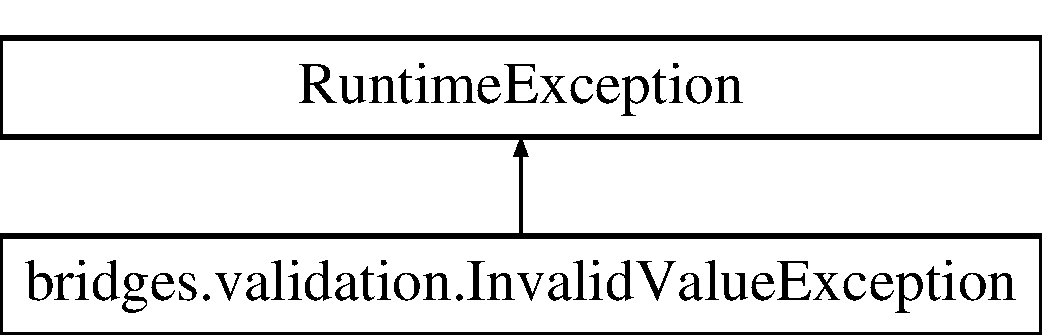
\includegraphics[height=2.000000cm]{classbridges_1_1validation_1_1_invalid_value_exception}
\end{center}
\end{figure}
\subsection*{Public Member Functions}
\begin{DoxyCompactItemize}
\item 
\mbox{\hyperlink{classbridges_1_1validation_1_1_invalid_value_exception_adf4c16bcef674454b87d8cc035efc75d}{Invalid\+Value\+Exception}} (String message)
\end{DoxyCompactItemize}


\subsection{Detailed Description}
Exception indicating invalid C\+SS values. Examples of uses for this include sizes with invalid units, and invalid colors. \begin{DoxyAuthor}{Author}
Sean Gallagher 
\end{DoxyAuthor}


\subsection{Constructor \& Destructor Documentation}
\mbox{\Hypertarget{classbridges_1_1validation_1_1_invalid_value_exception_adf4c16bcef674454b87d8cc035efc75d}\label{classbridges_1_1validation_1_1_invalid_value_exception_adf4c16bcef674454b87d8cc035efc75d}} 
\index{bridges\+::validation\+::\+Invalid\+Value\+Exception@{bridges\+::validation\+::\+Invalid\+Value\+Exception}!Invalid\+Value\+Exception@{Invalid\+Value\+Exception}}
\index{Invalid\+Value\+Exception@{Invalid\+Value\+Exception}!bridges\+::validation\+::\+Invalid\+Value\+Exception@{bridges\+::validation\+::\+Invalid\+Value\+Exception}}
\subsubsection{\texorpdfstring{Invalid\+Value\+Exception()}{InvalidValueException()}}
{\footnotesize\ttfamily bridges.\+validation.\+Invalid\+Value\+Exception.\+Invalid\+Value\+Exception (\begin{DoxyParamCaption}\item[{String}]{message }\end{DoxyParamCaption})}



The documentation for this class was generated from the following file\+:\begin{DoxyCompactItemize}
\item 
/\+Users/kalpathi/gr/bridges/client/java/bridges-\/17/src/main/java/bridges/validation/\mbox{\hyperlink{_invalid_value_exception_8java}{Invalid\+Value\+Exception.\+java}}\end{DoxyCompactItemize}

\hypertarget{classbridges_1_1base_1_1_kd_tree_element}{}\section{bridges.\+base.\+Kd\+Tree\+Element$<$ K, E $>$ Class Template Reference}
\label{classbridges_1_1base_1_1_kd_tree_element}\index{bridges.\+base.\+Kd\+Tree\+Element$<$ K, E $>$@{bridges.\+base.\+Kd\+Tree\+Element$<$ K, E $>$}}
Inheritance diagram for bridges.\+base.\+Kd\+Tree\+Element$<$ K, E $>$\+:\begin{figure}[H]
\begin{center}
\leavevmode
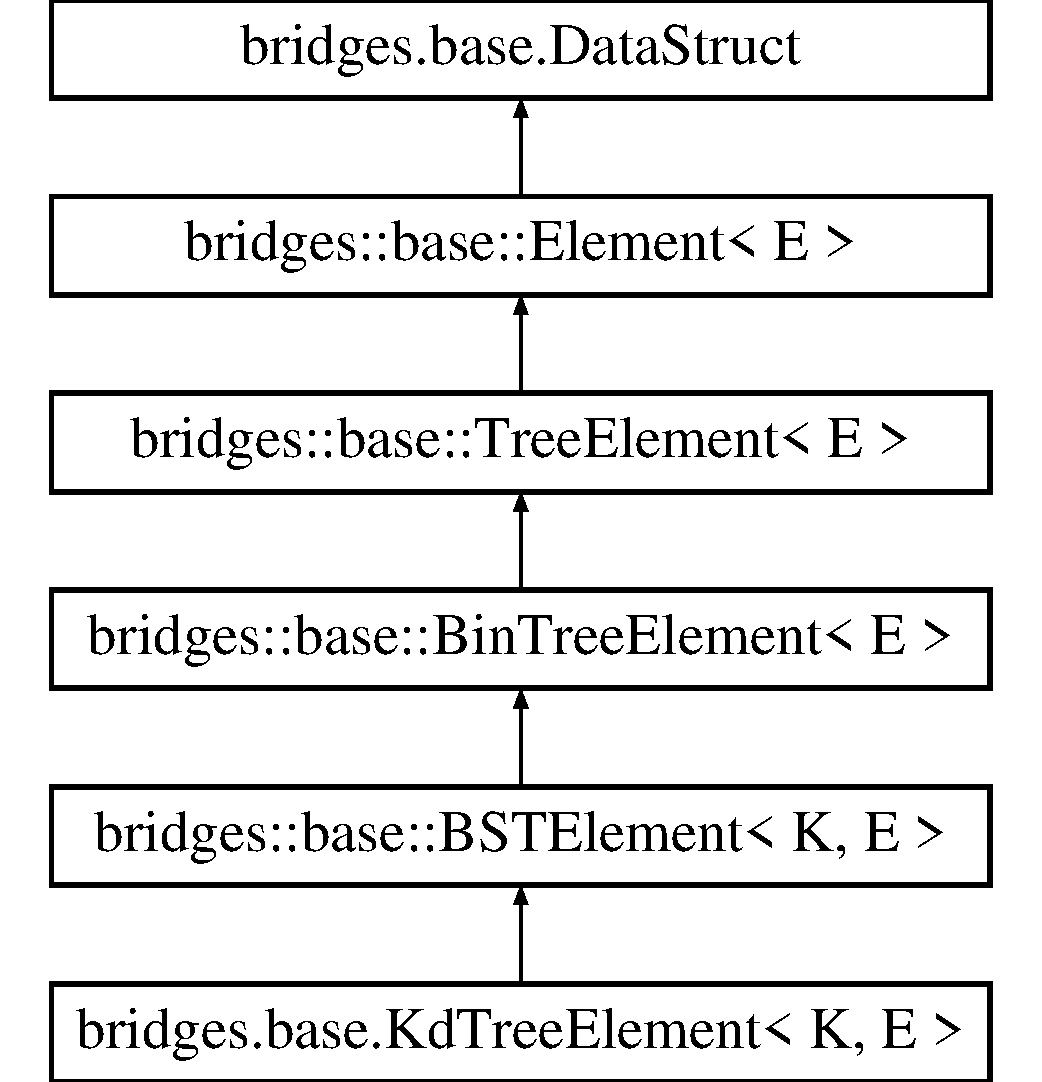
\includegraphics[height=6.000000cm]{classbridges_1_1base_1_1_kd_tree_element}
\end{center}
\end{figure}


\subsection{Detailed Description}
The This class can be used to create K-\/d Tree elements, derived from \hyperlink{classbridges_1_1base_1_1_b_s_t_element}{B\+S\+T\+Element}. K-\/D trees can be thought of as the spatial equivalent binary search trees and operate on multiple dimensions (2D and 3D are most common). These trees serve as a representation of the underlying geometrically defined spaces. Specialized versions of these trees include quadtrees and octrees, which subdivide into equal sized quadrants octants at each level, respectively. 

This class extends the \hyperlink{classbridges_1_1base_1_1_b_s_t_element}{B\+S\+T\+Element} class by adding a dimension property. It also includes a thickness property for displaying the partitioning lines generated by the convex decomposition. This thickness get passed to some constructor \hyperlink{classbridges_1_1base_1_1_kd_tree_element_a11cb855f1a151714ee24901a9e91e0da}{Kd\+Tree\+Element()} and to \hyperlink{classbridges_1_1base_1_1_kd_tree_element_a52412fc59c743a8a0ede057ed2451be9}{set\+Thickness()}. It is purely a graphical attribute.

convenient to generate visual representation to allow for use in a binary search tree implementation.

Generic Parameters\+: K that is the search key type -\/ this is usually a number, integer or float E the application data type

\begin{DoxyAuthor}{Author}
Kalpathi Subramanian 
\end{DoxyAuthor}
\begin{DoxyDate}{Date}
12/26/18, 7/12/19 
\end{DoxyDate}
\subsection*{Public Member Functions}
\begin{DoxyCompactItemize}
\item 
\hyperlink{classbridges_1_1base_1_1_kd_tree_element_a6acdec52089792d20747c10f56139217}{Kd\+Tree\+Element} (K k, int dim, float th, \hyperlink{classbridges_1_1base_1_1_kd_tree_element}{Kd\+Tree\+Element}$<$ K, E $>$ l, \hyperlink{classbridges_1_1base_1_1_kd_tree_element}{Kd\+Tree\+Element}$<$ K, E $>$ r, E val, String lab)
\item 
\hyperlink{classbridges_1_1base_1_1_kd_tree_element_a11cb855f1a151714ee24901a9e91e0da}{Kd\+Tree\+Element} ()
\item 
\hyperlink{classbridges_1_1base_1_1_kd_tree_element_a1db51371824c570a937aa2a78a6cc744}{Kd\+Tree\+Element} (E e, \hyperlink{classbridges_1_1base_1_1_kd_tree_element}{Kd\+Tree\+Element}$<$ K, E $>$ left, \hyperlink{classbridges_1_1base_1_1_kd_tree_element}{Kd\+Tree\+Element}$<$ K, E $>$ right)
\item 
\hyperlink{classbridges_1_1base_1_1_kd_tree_element_a504060ecd4861b5b4de851b72f5bfffc}{Kd\+Tree\+Element} (K key, E e, \hyperlink{classbridges_1_1base_1_1_kd_tree_element}{Kd\+Tree\+Element}$<$ K, E $>$ left, \hyperlink{classbridges_1_1base_1_1_kd_tree_element}{Kd\+Tree\+Element}$<$ K, E $>$ right)
\item 
\hyperlink{classbridges_1_1base_1_1_kd_tree_element_a671342818955bc2c49b326251fde8a1b}{Kd\+Tree\+Element} (E e)
\item 
\hyperlink{classbridges_1_1base_1_1_kd_tree_element_a438fde369fff7d1c34e2007db0e07239}{Kd\+Tree\+Element} (K key, int dim)
\item 
String \hyperlink{classbridges_1_1base_1_1_kd_tree_element_a56b98bd1f3e1e5c0c37519c4b3cf5ba2}{get\+Data\+Struct\+Type} ()
\item 
\hyperlink{classbridges_1_1base_1_1_kd_tree_element_a0ee0c961255e89e18529a5c951db53d9}{Kd\+Tree\+Element} (K key, E e)
\item 
\hyperlink{classbridges_1_1base_1_1_kd_tree_element_a74c3ed00a266215c716ebc945b8d1a69}{Kd\+Tree\+Element} (String label, E e)
\item 
\hyperlink{classbridges_1_1base_1_1_kd_tree_element_ad2c3a73929648e6afce54536790d94c9}{Kd\+Tree\+Element} (String label, K key, E e)
\item 
\hyperlink{classbridges_1_1base_1_1_kd_tree_element_ad8cd8e37105af65a6ae06e743be9aebe}{Kd\+Tree\+Element} (\hyperlink{classbridges_1_1base_1_1_kd_tree_element}{Kd\+Tree\+Element}$<$ K, E $>$ left, \hyperlink{classbridges_1_1base_1_1_kd_tree_element}{Kd\+Tree\+Element}$<$ K, E $>$ right)
\item 
int \hyperlink{classbridges_1_1base_1_1_kd_tree_element_a2469fcfe38e921ae48338ef1fd347c4a}{get\+Dimension} ()
\item 
void \hyperlink{classbridges_1_1base_1_1_kd_tree_element_af3fa89cbd20fc2c3f30784db16b6dec4}{set\+Dimension} (int dim)
\item 
float \hyperlink{classbridges_1_1base_1_1_kd_tree_element_a27c0b086af284210855ee5f1c90e7484}{get\+Thickness} ()
\item 
void \hyperlink{classbridges_1_1base_1_1_kd_tree_element_a52412fc59c743a8a0ede057ed2451be9}{set\+Thickness} (float th)
\item 
\hyperlink{classbridges_1_1base_1_1_kd_tree_element}{Kd\+Tree\+Element}$<$ K, E $>$ \hyperlink{classbridges_1_1base_1_1_kd_tree_element_a257367edc8f204c973eb277dcb5d37be}{get\+Left} ()
\item 
\hyperlink{classbridges_1_1base_1_1_kd_tree_element}{Kd\+Tree\+Element}$<$ K, E $>$ \hyperlink{classbridges_1_1base_1_1_kd_tree_element_a990694a36d44aba5f844f1752692c8e6}{get\+Right} ()
\item 
String \hyperlink{classbridges_1_1base_1_1_kd_tree_element_adf9bed8c71a7c257a1359c3c88b808f0}{get\+Element\+Representation} ()
\end{DoxyCompactItemize}
\subsection*{Additional Inherited Members}


\subsection{Constructor \& Destructor Documentation}
\mbox{\Hypertarget{classbridges_1_1base_1_1_kd_tree_element_a6acdec52089792d20747c10f56139217}\label{classbridges_1_1base_1_1_kd_tree_element_a6acdec52089792d20747c10f56139217}} 
\index{bridges\+::base\+::\+Kd\+Tree\+Element@{bridges\+::base\+::\+Kd\+Tree\+Element}!Kd\+Tree\+Element@{Kd\+Tree\+Element}}
\index{Kd\+Tree\+Element@{Kd\+Tree\+Element}!bridges\+::base\+::\+Kd\+Tree\+Element@{bridges\+::base\+::\+Kd\+Tree\+Element}}
\subsubsection{\texorpdfstring{Kd\+Tree\+Element()}{KdTreeElement()}\hspace{0.1cm}{\footnotesize\ttfamily [1/10]}}
{\footnotesize\ttfamily \hyperlink{classbridges_1_1base_1_1_kd_tree_element}{bridges.\+base.\+Kd\+Tree\+Element}$<$ K, E $>$.\hyperlink{classbridges_1_1base_1_1_kd_tree_element}{Kd\+Tree\+Element} (\begin{DoxyParamCaption}\item[{K}]{k,  }\item[{int}]{dim,  }\item[{float}]{th,  }\item[{\hyperlink{classbridges_1_1base_1_1_kd_tree_element}{Kd\+Tree\+Element}$<$ K, E $>$}]{l,  }\item[{\hyperlink{classbridges_1_1base_1_1_kd_tree_element}{Kd\+Tree\+Element}$<$ K, E $>$}]{r,  }\item[{E}]{val,  }\item[{String}]{lab }\end{DoxyParamCaption})}

Constructs a \hyperlink{classbridges_1_1base_1_1_kd_tree_element}{Kd\+Tree\+Element} with the provided value, label, key, left and right Kd\+Tree elements. The defaults will be used if not provided.


\begin{DoxyParams}{Parameters}
{\em k} & The key for ordering \\
\hline
{\em dim} & number of dimensions \\
\hline
{\em th} & thickness (used in rendering) \\
\hline
{\em l} & The left Kd\+Tree \hyperlink{classbridges_1_1base_1_1_element}{Element} \\
\hline
{\em r} & The right Kd\+Tree \hyperlink{classbridges_1_1base_1_1_element}{Element} \\
\hline
{\em val} & The data to hold \\
\hline
{\em lab} & The label to show \\
\hline
\end{DoxyParams}
\mbox{\Hypertarget{classbridges_1_1base_1_1_kd_tree_element_a11cb855f1a151714ee24901a9e91e0da}\label{classbridges_1_1base_1_1_kd_tree_element_a11cb855f1a151714ee24901a9e91e0da}} 
\index{bridges\+::base\+::\+Kd\+Tree\+Element@{bridges\+::base\+::\+Kd\+Tree\+Element}!Kd\+Tree\+Element@{Kd\+Tree\+Element}}
\index{Kd\+Tree\+Element@{Kd\+Tree\+Element}!bridges\+::base\+::\+Kd\+Tree\+Element@{bridges\+::base\+::\+Kd\+Tree\+Element}}
\subsubsection{\texorpdfstring{Kd\+Tree\+Element()}{KdTreeElement()}\hspace{0.1cm}{\footnotesize\ttfamily [2/10]}}
{\footnotesize\ttfamily \hyperlink{classbridges_1_1base_1_1_kd_tree_element}{bridges.\+base.\+Kd\+Tree\+Element}$<$ K, E $>$.\hyperlink{classbridges_1_1base_1_1_kd_tree_element}{Kd\+Tree\+Element} (\begin{DoxyParamCaption}{ }\end{DoxyParamCaption})}

Construct an empty \hyperlink{classbridges_1_1base_1_1_kd_tree_element}{Kd\+Tree\+Element} with no key assigned and left and right pointers set to null. \mbox{\Hypertarget{classbridges_1_1base_1_1_kd_tree_element_a1db51371824c570a937aa2a78a6cc744}\label{classbridges_1_1base_1_1_kd_tree_element_a1db51371824c570a937aa2a78a6cc744}} 
\index{bridges\+::base\+::\+Kd\+Tree\+Element@{bridges\+::base\+::\+Kd\+Tree\+Element}!Kd\+Tree\+Element@{Kd\+Tree\+Element}}
\index{Kd\+Tree\+Element@{Kd\+Tree\+Element}!bridges\+::base\+::\+Kd\+Tree\+Element@{bridges\+::base\+::\+Kd\+Tree\+Element}}
\subsubsection{\texorpdfstring{Kd\+Tree\+Element()}{KdTreeElement()}\hspace{0.1cm}{\footnotesize\ttfamily [3/10]}}
{\footnotesize\ttfamily \hyperlink{classbridges_1_1base_1_1_kd_tree_element}{bridges.\+base.\+Kd\+Tree\+Element}$<$ K, E $>$.\hyperlink{classbridges_1_1base_1_1_kd_tree_element}{Kd\+Tree\+Element} (\begin{DoxyParamCaption}\item[{E}]{e,  }\item[{\hyperlink{classbridges_1_1base_1_1_kd_tree_element}{Kd\+Tree\+Element}$<$ K, E $>$}]{left,  }\item[{\hyperlink{classbridges_1_1base_1_1_kd_tree_element}{Kd\+Tree\+Element}$<$ K, E $>$}]{right }\end{DoxyParamCaption})}

Construct a \hyperlink{classbridges_1_1base_1_1_kd_tree_element}{Kd\+Tree\+Element} holding an object \char`\"{}e\char`\"{} with a left pointer assigned to \char`\"{}left\char`\"{} and a right pointer assigned to \char`\"{}right\char`\"{}. 
\begin{DoxyParams}{Parameters}
{\em e} & the object that \hyperlink{classbridges_1_1base_1_1_kd_tree_element}{Kd\+Tree\+Element} is holding \\
\hline
{\em left} & the \hyperlink{classbridges_1_1base_1_1_kd_tree_element}{Kd\+Tree\+Element} that should be assigned to the left pointer \\
\hline
{\em right} & the \hyperlink{classbridges_1_1base_1_1_kd_tree_element}{Kd\+Tree\+Element} taht should be assigned to the right pointer \\
\hline
\end{DoxyParams}
\mbox{\Hypertarget{classbridges_1_1base_1_1_kd_tree_element_a504060ecd4861b5b4de851b72f5bfffc}\label{classbridges_1_1base_1_1_kd_tree_element_a504060ecd4861b5b4de851b72f5bfffc}} 
\index{bridges\+::base\+::\+Kd\+Tree\+Element@{bridges\+::base\+::\+Kd\+Tree\+Element}!Kd\+Tree\+Element@{Kd\+Tree\+Element}}
\index{Kd\+Tree\+Element@{Kd\+Tree\+Element}!bridges\+::base\+::\+Kd\+Tree\+Element@{bridges\+::base\+::\+Kd\+Tree\+Element}}
\subsubsection{\texorpdfstring{Kd\+Tree\+Element()}{KdTreeElement()}\hspace{0.1cm}{\footnotesize\ttfamily [4/10]}}
{\footnotesize\ttfamily \hyperlink{classbridges_1_1base_1_1_kd_tree_element}{bridges.\+base.\+Kd\+Tree\+Element}$<$ K, E $>$.\hyperlink{classbridges_1_1base_1_1_kd_tree_element}{Kd\+Tree\+Element} (\begin{DoxyParamCaption}\item[{K}]{key,  }\item[{E}]{e,  }\item[{\hyperlink{classbridges_1_1base_1_1_kd_tree_element}{Kd\+Tree\+Element}$<$ K, E $>$}]{left,  }\item[{\hyperlink{classbridges_1_1base_1_1_kd_tree_element}{Kd\+Tree\+Element}$<$ K, E $>$}]{right }\end{DoxyParamCaption})}

Construct a \hyperlink{classbridges_1_1base_1_1_kd_tree_element}{Kd\+Tree\+Element} with a key \char`\"{}key\char`\"{}, holding an object \char`\"{}e\char`\"{} with a left pointer assigned to \char`\"{}left\char`\"{} and a right pointer assigned to \char`\"{}right\char`\"{}.


\begin{DoxyParams}{Parameters}
{\em key} & the key to be used in a binary search tree implementation \\
\hline
{\em e} & the object this \hyperlink{classbridges_1_1base_1_1_kd_tree_element}{Kd\+Tree\+Element} is holding \\
\hline
{\em left} & the \hyperlink{classbridges_1_1base_1_1_kd_tree_element}{Kd\+Tree\+Element} that should be assigned to the left pointer \\
\hline
{\em right} & the \hyperlink{classbridges_1_1base_1_1_kd_tree_element}{Kd\+Tree\+Element} that should be assigned to the right pointer \\
\hline
\end{DoxyParams}
\mbox{\Hypertarget{classbridges_1_1base_1_1_kd_tree_element_a671342818955bc2c49b326251fde8a1b}\label{classbridges_1_1base_1_1_kd_tree_element_a671342818955bc2c49b326251fde8a1b}} 
\index{bridges\+::base\+::\+Kd\+Tree\+Element@{bridges\+::base\+::\+Kd\+Tree\+Element}!Kd\+Tree\+Element@{Kd\+Tree\+Element}}
\index{Kd\+Tree\+Element@{Kd\+Tree\+Element}!bridges\+::base\+::\+Kd\+Tree\+Element@{bridges\+::base\+::\+Kd\+Tree\+Element}}
\subsubsection{\texorpdfstring{Kd\+Tree\+Element()}{KdTreeElement()}\hspace{0.1cm}{\footnotesize\ttfamily [5/10]}}
{\footnotesize\ttfamily \hyperlink{classbridges_1_1base_1_1_kd_tree_element}{bridges.\+base.\+Kd\+Tree\+Element}$<$ K, E $>$.\hyperlink{classbridges_1_1base_1_1_kd_tree_element}{Kd\+Tree\+Element} (\begin{DoxyParamCaption}\item[{E}]{e }\end{DoxyParamCaption})}

Construct a \hyperlink{classbridges_1_1base_1_1_kd_tree_element}{Kd\+Tree\+Element} holding the object \char`\"{}e\char`\"{}, with no key assigned and left and right pointers set to null.


\begin{DoxyParams}{Parameters}
{\em e} & the object this \hyperlink{classbridges_1_1base_1_1_kd_tree_element}{Kd\+Tree\+Element} is holding \\
\hline
\end{DoxyParams}
\mbox{\Hypertarget{classbridges_1_1base_1_1_kd_tree_element_a438fde369fff7d1c34e2007db0e07239}\label{classbridges_1_1base_1_1_kd_tree_element_a438fde369fff7d1c34e2007db0e07239}} 
\index{bridges\+::base\+::\+Kd\+Tree\+Element@{bridges\+::base\+::\+Kd\+Tree\+Element}!Kd\+Tree\+Element@{Kd\+Tree\+Element}}
\index{Kd\+Tree\+Element@{Kd\+Tree\+Element}!bridges\+::base\+::\+Kd\+Tree\+Element@{bridges\+::base\+::\+Kd\+Tree\+Element}}
\subsubsection{\texorpdfstring{Kd\+Tree\+Element()}{KdTreeElement()}\hspace{0.1cm}{\footnotesize\ttfamily [6/10]}}
{\footnotesize\ttfamily \hyperlink{classbridges_1_1base_1_1_kd_tree_element}{bridges.\+base.\+Kd\+Tree\+Element}$<$ K, E $>$.\hyperlink{classbridges_1_1base_1_1_kd_tree_element}{Kd\+Tree\+Element} (\begin{DoxyParamCaption}\item[{K}]{key,  }\item[{int}]{dim }\end{DoxyParamCaption})}

Construct a \hyperlink{classbridges_1_1base_1_1_kd_tree_element}{Kd\+Tree\+Element} given the key and dimension


\begin{DoxyParams}{Parameters}
{\em key} & the key to be used in a binary search tree implementation \\
\hline
{\em dim} & the dimension of partitioning \\
\hline
\end{DoxyParams}
\mbox{\Hypertarget{classbridges_1_1base_1_1_kd_tree_element_a0ee0c961255e89e18529a5c951db53d9}\label{classbridges_1_1base_1_1_kd_tree_element_a0ee0c961255e89e18529a5c951db53d9}} 
\index{bridges\+::base\+::\+Kd\+Tree\+Element@{bridges\+::base\+::\+Kd\+Tree\+Element}!Kd\+Tree\+Element@{Kd\+Tree\+Element}}
\index{Kd\+Tree\+Element@{Kd\+Tree\+Element}!bridges\+::base\+::\+Kd\+Tree\+Element@{bridges\+::base\+::\+Kd\+Tree\+Element}}
\subsubsection{\texorpdfstring{Kd\+Tree\+Element()}{KdTreeElement()}\hspace{0.1cm}{\footnotesize\ttfamily [7/10]}}
{\footnotesize\ttfamily \hyperlink{classbridges_1_1base_1_1_kd_tree_element}{bridges.\+base.\+Kd\+Tree\+Element}$<$ K, E $>$.\hyperlink{classbridges_1_1base_1_1_kd_tree_element}{Kd\+Tree\+Element} (\begin{DoxyParamCaption}\item[{K}]{key,  }\item[{E}]{e }\end{DoxyParamCaption})}

Construct a \hyperlink{classbridges_1_1base_1_1_kd_tree_element}{Kd\+Tree\+Element} holding the object \char`\"{}e\char`\"{}, with key \char`\"{}key\char`\"{} assigned and left and right pointers set to null. 
\begin{DoxyParams}{Parameters}
{\em key} & the key to be used in a binary search tree implementation \\
\hline
{\em e} & the object this \hyperlink{classbridges_1_1base_1_1_kd_tree_element}{Kd\+Tree\+Element} is holding \\
\hline
\end{DoxyParams}
\mbox{\Hypertarget{classbridges_1_1base_1_1_kd_tree_element_a74c3ed00a266215c716ebc945b8d1a69}\label{classbridges_1_1base_1_1_kd_tree_element_a74c3ed00a266215c716ebc945b8d1a69}} 
\index{bridges\+::base\+::\+Kd\+Tree\+Element@{bridges\+::base\+::\+Kd\+Tree\+Element}!Kd\+Tree\+Element@{Kd\+Tree\+Element}}
\index{Kd\+Tree\+Element@{Kd\+Tree\+Element}!bridges\+::base\+::\+Kd\+Tree\+Element@{bridges\+::base\+::\+Kd\+Tree\+Element}}
\subsubsection{\texorpdfstring{Kd\+Tree\+Element()}{KdTreeElement()}\hspace{0.1cm}{\footnotesize\ttfamily [8/10]}}
{\footnotesize\ttfamily \hyperlink{classbridges_1_1base_1_1_kd_tree_element}{bridges.\+base.\+Kd\+Tree\+Element}$<$ K, E $>$.\hyperlink{classbridges_1_1base_1_1_kd_tree_element}{Kd\+Tree\+Element} (\begin{DoxyParamCaption}\item[{String}]{label,  }\item[{E}]{e }\end{DoxyParamCaption})}

Construct a \hyperlink{classbridges_1_1base_1_1_kd_tree_element}{Kd\+Tree\+Element} holding the object \char`\"{}e\char`\"{}, with label set to \char`\"{}label\char`\"{}, with no key assigned, and left and right pointers set to null. 
\begin{DoxyParams}{Parameters}
{\em label} & the label of \hyperlink{classbridges_1_1base_1_1_kd_tree_element}{Kd\+Tree\+Element} that shows up on the Bridges visualization \\
\hline
{\em e} & the object this \hyperlink{classbridges_1_1base_1_1_kd_tree_element}{Kd\+Tree\+Element} is holding \\
\hline
\end{DoxyParams}
\mbox{\Hypertarget{classbridges_1_1base_1_1_kd_tree_element_ad2c3a73929648e6afce54536790d94c9}\label{classbridges_1_1base_1_1_kd_tree_element_ad2c3a73929648e6afce54536790d94c9}} 
\index{bridges\+::base\+::\+Kd\+Tree\+Element@{bridges\+::base\+::\+Kd\+Tree\+Element}!Kd\+Tree\+Element@{Kd\+Tree\+Element}}
\index{Kd\+Tree\+Element@{Kd\+Tree\+Element}!bridges\+::base\+::\+Kd\+Tree\+Element@{bridges\+::base\+::\+Kd\+Tree\+Element}}
\subsubsection{\texorpdfstring{Kd\+Tree\+Element()}{KdTreeElement()}\hspace{0.1cm}{\footnotesize\ttfamily [9/10]}}
{\footnotesize\ttfamily \hyperlink{classbridges_1_1base_1_1_kd_tree_element}{bridges.\+base.\+Kd\+Tree\+Element}$<$ K, E $>$.\hyperlink{classbridges_1_1base_1_1_kd_tree_element}{Kd\+Tree\+Element} (\begin{DoxyParamCaption}\item[{String}]{label,  }\item[{K}]{key,  }\item[{E}]{e }\end{DoxyParamCaption})}

Construct a \hyperlink{classbridges_1_1base_1_1_kd_tree_element}{Kd\+Tree\+Element} holding the object \char`\"{}e\char`\"{}, with label set to \char`\"{}label\char`\"{}, with \char`\"{}key\char`\"{} assigned to key, and left and right pointers set to null.


\begin{DoxyParams}{Parameters}
{\em label} & the label of \hyperlink{classbridges_1_1base_1_1_kd_tree_element}{Kd\+Tree\+Element} that shows up on the Bridges visualization \\
\hline
{\em key} & the key to be used in a binary search tree implementation \\
\hline
{\em e} & the object this \hyperlink{classbridges_1_1base_1_1_kd_tree_element}{Kd\+Tree\+Element} is holding \\
\hline
\end{DoxyParams}
\mbox{\Hypertarget{classbridges_1_1base_1_1_kd_tree_element_ad8cd8e37105af65a6ae06e743be9aebe}\label{classbridges_1_1base_1_1_kd_tree_element_ad8cd8e37105af65a6ae06e743be9aebe}} 
\index{bridges\+::base\+::\+Kd\+Tree\+Element@{bridges\+::base\+::\+Kd\+Tree\+Element}!Kd\+Tree\+Element@{Kd\+Tree\+Element}}
\index{Kd\+Tree\+Element@{Kd\+Tree\+Element}!bridges\+::base\+::\+Kd\+Tree\+Element@{bridges\+::base\+::\+Kd\+Tree\+Element}}
\subsubsection{\texorpdfstring{Kd\+Tree\+Element()}{KdTreeElement()}\hspace{0.1cm}{\footnotesize\ttfamily [10/10]}}
{\footnotesize\ttfamily \hyperlink{classbridges_1_1base_1_1_kd_tree_element}{bridges.\+base.\+Kd\+Tree\+Element}$<$ K, E $>$.\hyperlink{classbridges_1_1base_1_1_kd_tree_element}{Kd\+Tree\+Element} (\begin{DoxyParamCaption}\item[{\hyperlink{classbridges_1_1base_1_1_kd_tree_element}{Kd\+Tree\+Element}$<$ K, E $>$}]{left,  }\item[{\hyperlink{classbridges_1_1base_1_1_kd_tree_element}{Kd\+Tree\+Element}$<$ K, E $>$}]{right }\end{DoxyParamCaption})}

Construct an empty \hyperlink{classbridges_1_1base_1_1_kd_tree_element}{Kd\+Tree\+Element}, with no key assigned, and left and right pointers set to null. 
\begin{DoxyParams}{Parameters}
{\em left} & the \hyperlink{classbridges_1_1base_1_1_kd_tree_element}{Kd\+Tree\+Element} that should be assigned to the left pointer \\
\hline
{\em right} & the \hyperlink{classbridges_1_1base_1_1_kd_tree_element}{Kd\+Tree\+Element} that should be assigned to the right pointer \\
\hline
\end{DoxyParams}


\subsection{Member Function Documentation}
\mbox{\Hypertarget{classbridges_1_1base_1_1_kd_tree_element_a56b98bd1f3e1e5c0c37519c4b3cf5ba2}\label{classbridges_1_1base_1_1_kd_tree_element_a56b98bd1f3e1e5c0c37519c4b3cf5ba2}} 
\index{bridges\+::base\+::\+Kd\+Tree\+Element@{bridges\+::base\+::\+Kd\+Tree\+Element}!get\+Data\+Struct\+Type@{get\+Data\+Struct\+Type}}
\index{get\+Data\+Struct\+Type@{get\+Data\+Struct\+Type}!bridges\+::base\+::\+Kd\+Tree\+Element@{bridges\+::base\+::\+Kd\+Tree\+Element}}
\subsubsection{\texorpdfstring{get\+Data\+Struct\+Type()}{getDataStructType()}}
{\footnotesize\ttfamily String \hyperlink{classbridges_1_1base_1_1_kd_tree_element}{bridges.\+base.\+Kd\+Tree\+Element}$<$ K, E $>$.get\+Data\+Struct\+Type (\begin{DoxyParamCaption}{ }\end{DoxyParamCaption})}

This method gets the data structure type

\begin{DoxyReturn}{Returns}
The date structure type as a string 
\end{DoxyReturn}
\mbox{\Hypertarget{classbridges_1_1base_1_1_kd_tree_element_a2469fcfe38e921ae48338ef1fd347c4a}\label{classbridges_1_1base_1_1_kd_tree_element_a2469fcfe38e921ae48338ef1fd347c4a}} 
\index{bridges\+::base\+::\+Kd\+Tree\+Element@{bridges\+::base\+::\+Kd\+Tree\+Element}!get\+Dimension@{get\+Dimension}}
\index{get\+Dimension@{get\+Dimension}!bridges\+::base\+::\+Kd\+Tree\+Element@{bridges\+::base\+::\+Kd\+Tree\+Element}}
\subsubsection{\texorpdfstring{get\+Dimension()}{getDimension()}}
{\footnotesize\ttfamily int \hyperlink{classbridges_1_1base_1_1_kd_tree_element}{bridges.\+base.\+Kd\+Tree\+Element}$<$ K, E $>$.get\+Dimension (\begin{DoxyParamCaption}{ }\end{DoxyParamCaption})}

Return the partitioning dimension

\begin{DoxyReturn}{Returns}
the partitioning dimension of this \hyperlink{classbridges_1_1base_1_1_kd_tree_element}{Kd\+Tree\+Element} 
\end{DoxyReturn}
\mbox{\Hypertarget{classbridges_1_1base_1_1_kd_tree_element_adf9bed8c71a7c257a1359c3c88b808f0}\label{classbridges_1_1base_1_1_kd_tree_element_adf9bed8c71a7c257a1359c3c88b808f0}} 
\index{bridges\+::base\+::\+Kd\+Tree\+Element@{bridges\+::base\+::\+Kd\+Tree\+Element}!get\+Element\+Representation@{get\+Element\+Representation}}
\index{get\+Element\+Representation@{get\+Element\+Representation}!bridges\+::base\+::\+Kd\+Tree\+Element@{bridges\+::base\+::\+Kd\+Tree\+Element}}
\subsubsection{\texorpdfstring{get\+Element\+Representation()}{getElementRepresentation()}}
{\footnotesize\ttfamily String \hyperlink{classbridges_1_1base_1_1_kd_tree_element}{bridges.\+base.\+Kd\+Tree\+Element}$<$ K, E $>$.get\+Element\+Representation (\begin{DoxyParamCaption}{ }\end{DoxyParamCaption})}

Augment the element with the \char`\"{}height\char`\"{} and \char`\"{}balance factor\char`\"{} fields.

\begin{DoxyReturn}{Returns}
the augmented J\+S\+ON string 
\end{DoxyReturn}
\mbox{\Hypertarget{classbridges_1_1base_1_1_kd_tree_element_a257367edc8f204c973eb277dcb5d37be}\label{classbridges_1_1base_1_1_kd_tree_element_a257367edc8f204c973eb277dcb5d37be}} 
\index{bridges\+::base\+::\+Kd\+Tree\+Element@{bridges\+::base\+::\+Kd\+Tree\+Element}!get\+Left@{get\+Left}}
\index{get\+Left@{get\+Left}!bridges\+::base\+::\+Kd\+Tree\+Element@{bridges\+::base\+::\+Kd\+Tree\+Element}}
\subsubsection{\texorpdfstring{get\+Left()}{getLeft()}}
{\footnotesize\ttfamily \hyperlink{classbridges_1_1base_1_1_kd_tree_element}{Kd\+Tree\+Element}$<$K, E$>$ \hyperlink{classbridges_1_1base_1_1_kd_tree_element}{bridges.\+base.\+Kd\+Tree\+Element}$<$ K, E $>$.get\+Left (\begin{DoxyParamCaption}{ }\end{DoxyParamCaption})}

Return the left child

\begin{DoxyReturn}{Returns}
the left child of this \hyperlink{classbridges_1_1base_1_1_kd_tree_element}{Kd\+Tree\+Element} 
\end{DoxyReturn}
\mbox{\Hypertarget{classbridges_1_1base_1_1_kd_tree_element_a990694a36d44aba5f844f1752692c8e6}\label{classbridges_1_1base_1_1_kd_tree_element_a990694a36d44aba5f844f1752692c8e6}} 
\index{bridges\+::base\+::\+Kd\+Tree\+Element@{bridges\+::base\+::\+Kd\+Tree\+Element}!get\+Right@{get\+Right}}
\index{get\+Right@{get\+Right}!bridges\+::base\+::\+Kd\+Tree\+Element@{bridges\+::base\+::\+Kd\+Tree\+Element}}
\subsubsection{\texorpdfstring{get\+Right()}{getRight()}}
{\footnotesize\ttfamily \hyperlink{classbridges_1_1base_1_1_kd_tree_element}{Kd\+Tree\+Element}$<$K, E$>$ \hyperlink{classbridges_1_1base_1_1_kd_tree_element}{bridges.\+base.\+Kd\+Tree\+Element}$<$ K, E $>$.get\+Right (\begin{DoxyParamCaption}{ }\end{DoxyParamCaption})}

Return the right child

\begin{DoxyReturn}{Returns}
the right child of this \hyperlink{classbridges_1_1base_1_1_kd_tree_element}{Kd\+Tree\+Element} 
\end{DoxyReturn}
\mbox{\Hypertarget{classbridges_1_1base_1_1_kd_tree_element_a27c0b086af284210855ee5f1c90e7484}\label{classbridges_1_1base_1_1_kd_tree_element_a27c0b086af284210855ee5f1c90e7484}} 
\index{bridges\+::base\+::\+Kd\+Tree\+Element@{bridges\+::base\+::\+Kd\+Tree\+Element}!get\+Thickness@{get\+Thickness}}
\index{get\+Thickness@{get\+Thickness}!bridges\+::base\+::\+Kd\+Tree\+Element@{bridges\+::base\+::\+Kd\+Tree\+Element}}
\subsubsection{\texorpdfstring{get\+Thickness()}{getThickness()}}
{\footnotesize\ttfamily float \hyperlink{classbridges_1_1base_1_1_kd_tree_element}{bridges.\+base.\+Kd\+Tree\+Element}$<$ K, E $>$.get\+Thickness (\begin{DoxyParamCaption}{ }\end{DoxyParamCaption})}

Return the thickness of the Kdtree\+Element; thickness is used in the visualization to draw the partitioning lines

\begin{DoxyReturn}{Returns}
the thickness of this \hyperlink{classbridges_1_1base_1_1_kd_tree_element}{Kd\+Tree\+Element} 
\end{DoxyReturn}
\mbox{\Hypertarget{classbridges_1_1base_1_1_kd_tree_element_af3fa89cbd20fc2c3f30784db16b6dec4}\label{classbridges_1_1base_1_1_kd_tree_element_af3fa89cbd20fc2c3f30784db16b6dec4}} 
\index{bridges\+::base\+::\+Kd\+Tree\+Element@{bridges\+::base\+::\+Kd\+Tree\+Element}!set\+Dimension@{set\+Dimension}}
\index{set\+Dimension@{set\+Dimension}!bridges\+::base\+::\+Kd\+Tree\+Element@{bridges\+::base\+::\+Kd\+Tree\+Element}}
\subsubsection{\texorpdfstring{set\+Dimension()}{setDimension()}}
{\footnotesize\ttfamily void \hyperlink{classbridges_1_1base_1_1_kd_tree_element}{bridges.\+base.\+Kd\+Tree\+Element}$<$ K, E $>$.set\+Dimension (\begin{DoxyParamCaption}\item[{int}]{dim }\end{DoxyParamCaption})}

Set the dimension of the Kd\+Tre\+Element to key 
\begin{DoxyParams}{Parameters}
{\em dim} & the dimension to set \\
\hline
\end{DoxyParams}
\mbox{\Hypertarget{classbridges_1_1base_1_1_kd_tree_element_a52412fc59c743a8a0ede057ed2451be9}\label{classbridges_1_1base_1_1_kd_tree_element_a52412fc59c743a8a0ede057ed2451be9}} 
\index{bridges\+::base\+::\+Kd\+Tree\+Element@{bridges\+::base\+::\+Kd\+Tree\+Element}!set\+Thickness@{set\+Thickness}}
\index{set\+Thickness@{set\+Thickness}!bridges\+::base\+::\+Kd\+Tree\+Element@{bridges\+::base\+::\+Kd\+Tree\+Element}}
\subsubsection{\texorpdfstring{set\+Thickness()}{setThickness()}}
{\footnotesize\ttfamily void \hyperlink{classbridges_1_1base_1_1_kd_tree_element}{bridges.\+base.\+Kd\+Tree\+Element}$<$ K, E $>$.set\+Thickness (\begin{DoxyParamCaption}\item[{float}]{th }\end{DoxyParamCaption})}

Set the thickness of the \hyperlink{classbridges_1_1base_1_1_kd_tree_element}{Kd\+Tree\+Element} 
\begin{DoxyParams}{Parameters}
{\em th} & thickness of the partitioner to set thickness is used in the visualization to draw the partitioning lines \\
\hline
\end{DoxyParams}


The documentation for this class was generated from the following file\+:\begin{DoxyCompactItemize}
\item 
/home/erik/work/bridges/bridges-\/java/src/main/java/bridges/base/\hyperlink{_kd_tree_element_8java}{Kd\+Tree\+Element.\+java}\end{DoxyCompactItemize}

\hypertarget{interfacebridges_1_1connect_1_1_keypress_listener}{}\section{bridges.\+connect.\+Keypress\+Listener Interface Reference}
\label{interfacebridges_1_1connect_1_1_keypress_listener}\index{bridges.\+connect.\+Keypress\+Listener@{bridges.\+connect.\+Keypress\+Listener}}
Inheritance diagram for bridges.\+connect.\+Keypress\+Listener\+:\begin{figure}[H]
\begin{center}
\leavevmode
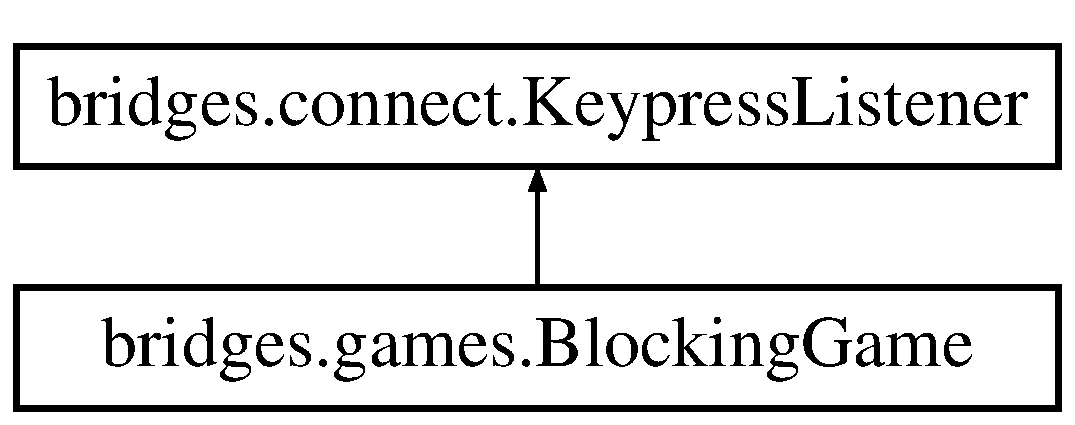
\includegraphics[height=2.000000cm]{interfacebridges_1_1connect_1_1_keypress_listener}
\end{center}
\end{figure}
\subsection*{Public Member Functions}
\begin{DoxyCompactItemize}
\item 
void \mbox{\hyperlink{interfacebridges_1_1connect_1_1_keypress_listener_af713d94f36bce842f39ce0aea4db8da6}{keypress}} (J\+S\+O\+N\+Object keypress)
\end{DoxyCompactItemize}


\subsection{Member Function Documentation}
\mbox{\Hypertarget{interfacebridges_1_1connect_1_1_keypress_listener_af713d94f36bce842f39ce0aea4db8da6}\label{interfacebridges_1_1connect_1_1_keypress_listener_af713d94f36bce842f39ce0aea4db8da6}} 
\index{bridges\+::connect\+::\+Keypress\+Listener@{bridges\+::connect\+::\+Keypress\+Listener}!keypress@{keypress}}
\index{keypress@{keypress}!bridges\+::connect\+::\+Keypress\+Listener@{bridges\+::connect\+::\+Keypress\+Listener}}
\subsubsection{\texorpdfstring{keypress()}{keypress()}}
{\footnotesize\ttfamily void bridges.\+connect.\+Keypress\+Listener.\+keypress (\begin{DoxyParamCaption}\item[{J\+S\+O\+N\+Object}]{keypress }\end{DoxyParamCaption})}



Implemented in \mbox{\hyperlink{classbridges_1_1games_1_1_blocking_game_a53b1b38826785ee7c7a13f486b7b72ba}{bridges.\+games.\+Blocking\+Game}}.



The documentation for this interface was generated from the following file\+:\begin{DoxyCompactItemize}
\item 
/\+Users/kalpathi/gr/bridges/client/java/src/main/java/bridges/connect/\mbox{\hyperlink{_keypress_listener_8java}{Keypress\+Listener.\+java}}\end{DoxyCompactItemize}

\hypertarget{classbridges_1_1base_1_1_label}{}\section{bridges.\+base.\+Label Class Reference}
\label{classbridges_1_1base_1_1_label}\index{bridges.base.Label@{bridges.base.Label}}


This is a superclass in B\+R\+I\+D\+G\+ES for deriving a number of Shape objects for use in a Shape\+Collection. Shapes correspond to a simplified subset of S\+VG paths and shapes for custom visual representations in B\+R\+I\+D\+G\+ES.  


Inheritance diagram for bridges.\+base.\+Label\+:\begin{figure}[H]
\begin{center}
\leavevmode
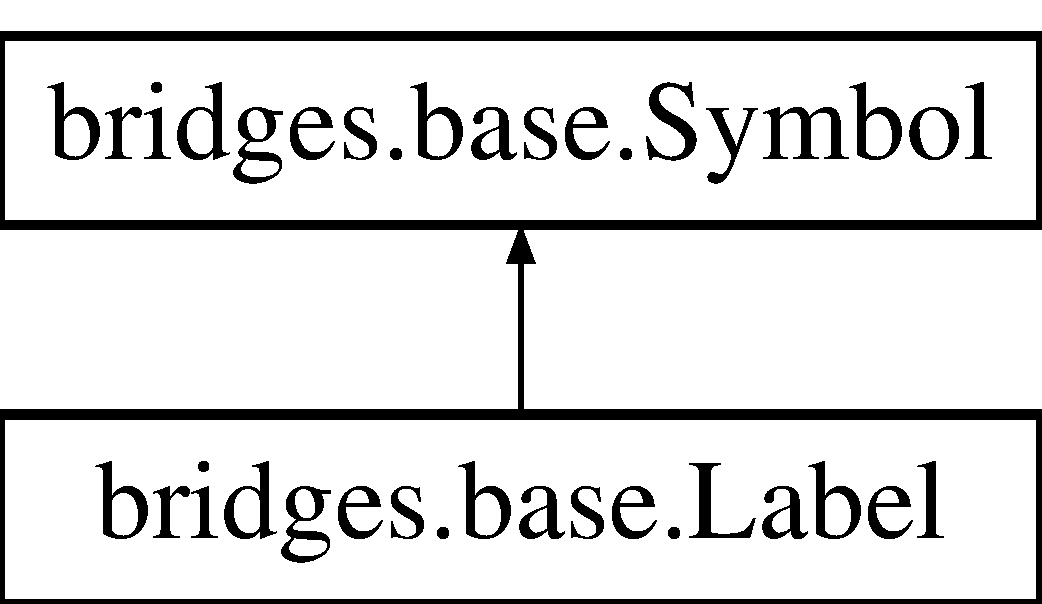
\includegraphics[height=3.000000cm]{classbridges_1_1base_1_1_label}
\end{center}
\end{figure}
\subsection*{Public Member Functions}
\begin{DoxyCompactItemize}
\item 
\mbox{\hyperlink{classbridges_1_1base_1_1_label_adaed1c29dc02eb0f77d772b256b9eae4}{Label}} ()
\item 
\mbox{\hyperlink{classbridges_1_1base_1_1_label_a0ffb2cdafae3f2c21e0925f2fe23df87}{Label}} (String \mbox{\hyperlink{classbridges_1_1base_1_1_symbol_ad2adcc82e6a96c2f3c465702502655e9}{label}})
\item 
\mbox{\hyperlink{classbridges_1_1base_1_1_label}{Label}} \mbox{\hyperlink{classbridges_1_1base_1_1_label_ab5f2d60e519db2499f326c4ccb967b25}{set\+Font\+Size}} (Integer size)
\item 
Float \mbox{[}$\,$\mbox{]} \mbox{\hyperlink{classbridges_1_1base_1_1_label_a9df9f801df020ba601a7bd33f38b4b0f}{get\+Dimensions}} ()
\item 
J\+S\+O\+N\+Object \mbox{\hyperlink{classbridges_1_1base_1_1_label_a6befc6655ce36868213be289571c6315}{get\+J\+S\+O\+N\+Representation}} ()
\end{DoxyCompactItemize}
\subsection*{Additional Inherited Members}


\subsection{Detailed Description}
This is a superclass in B\+R\+I\+D\+G\+ES for deriving a number of Shape objects for use in a Shape\+Collection. Shapes correspond to a simplified subset of S\+VG paths and shapes for custom visual representations in B\+R\+I\+D\+G\+ES. 

\begin{DoxyAuthor}{Author}
David Burlinson 
\end{DoxyAuthor}


\subsection{Constructor \& Destructor Documentation}
\mbox{\Hypertarget{classbridges_1_1base_1_1_label_adaed1c29dc02eb0f77d772b256b9eae4}\label{classbridges_1_1base_1_1_label_adaed1c29dc02eb0f77d772b256b9eae4}} 
\index{bridges.base.Label@{bridges.base.Label}!Label@{Label}}
\index{Label@{Label}!bridges.base.Label@{bridges.base.Label}}
\subsubsection{\texorpdfstring{Label()}{Label()}\hspace{0.1cm}{\footnotesize\ttfamily [1/2]}}
{\footnotesize\ttfamily bridges.\+base.\+Label.\+Label (\begin{DoxyParamCaption}{ }\end{DoxyParamCaption})}

\mbox{\Hypertarget{classbridges_1_1base_1_1_label_a0ffb2cdafae3f2c21e0925f2fe23df87}\label{classbridges_1_1base_1_1_label_a0ffb2cdafae3f2c21e0925f2fe23df87}} 
\index{bridges.base.Label@{bridges.base.Label}!Label@{Label}}
\index{Label@{Label}!bridges.base.Label@{bridges.base.Label}}
\subsubsection{\texorpdfstring{Label()}{Label()}\hspace{0.1cm}{\footnotesize\ttfamily [2/2]}}
{\footnotesize\ttfamily bridges.\+base.\+Label.\+Label (\begin{DoxyParamCaption}\item[{String}]{label }\end{DoxyParamCaption})}



\subsection{Member Function Documentation}
\mbox{\Hypertarget{classbridges_1_1base_1_1_label_a9df9f801df020ba601a7bd33f38b4b0f}\label{classbridges_1_1base_1_1_label_a9df9f801df020ba601a7bd33f38b4b0f}} 
\index{bridges.base.Label@{bridges.base.Label}!getDimensions@{getDimensions}}
\index{getDimensions@{getDimensions}!bridges.base.Label@{bridges.base.Label}}
\subsubsection{\texorpdfstring{getDimensions()}{getDimensions()}}
{\footnotesize\ttfamily Float \mbox{[}$\,$\mbox{]} bridges.\+base.\+Label.\+get\+Dimensions (\begin{DoxyParamCaption}{ }\end{DoxyParamCaption})}

\mbox{\Hypertarget{classbridges_1_1base_1_1_label_a6befc6655ce36868213be289571c6315}\label{classbridges_1_1base_1_1_label_a6befc6655ce36868213be289571c6315}} 
\index{bridges.base.Label@{bridges.base.Label}!getJSONRepresentation@{getJSONRepresentation}}
\index{getJSONRepresentation@{getJSONRepresentation}!bridges.base.Label@{bridges.base.Label}}
\subsubsection{\texorpdfstring{getJSONRepresentation()}{getJSONRepresentation()}}
{\footnotesize\ttfamily J\+S\+O\+N\+Object bridges.\+base.\+Label.\+get\+J\+S\+O\+N\+Representation (\begin{DoxyParamCaption}{ }\end{DoxyParamCaption})}

Internal code for getting the properties of the Shape object. It produces (without the spaces or newlines)\+: \{ \char`\"{}name\char`\"{}\+: \char`\"{}\+Some label\char`\"{}, \char`\"{}other C\+S\+S properties like color\char`\"{}\+: any\+\_\+\+J\+S\+O\+N\+\_\+value \} \begin{DoxyReturn}{Returns}
the encoded J\+S\+ON string 
\end{DoxyReturn}
\mbox{\Hypertarget{classbridges_1_1base_1_1_label_ab5f2d60e519db2499f326c4ccb967b25}\label{classbridges_1_1base_1_1_label_ab5f2d60e519db2499f326c4ccb967b25}} 
\index{bridges.base.Label@{bridges.base.Label}!setFontSize@{setFontSize}}
\index{setFontSize@{setFontSize}!bridges.base.Label@{bridges.base.Label}}
\subsubsection{\texorpdfstring{setFontSize()}{setFontSize()}}
{\footnotesize\ttfamily \mbox{\hyperlink{classbridges_1_1base_1_1_label}{Label}} bridges.\+base.\+Label.\+set\+Font\+Size (\begin{DoxyParamCaption}\item[{Integer}]{size }\end{DoxyParamCaption})}



The documentation for this class was generated from the following file\+:\begin{DoxyCompactItemize}
\item 
/\+Users/kalpathi/gr/bridges/java/src/main/java/bridges/base/\mbox{\hyperlink{_label_8java}{Label.\+java}}\end{DoxyCompactItemize}

\hypertarget{classbridges_1_1base_1_1_line_chart}{}\section{bridges.\+base.\+Line\+Chart Class Reference}
\label{classbridges_1_1base_1_1_line_chart}\index{bridges.\+base.\+Line\+Chart@{bridges.\+base.\+Line\+Chart}}
Inheritance diagram for bridges.\+base.\+Line\+Chart\+:\begin{figure}[H]
\begin{center}
\leavevmode
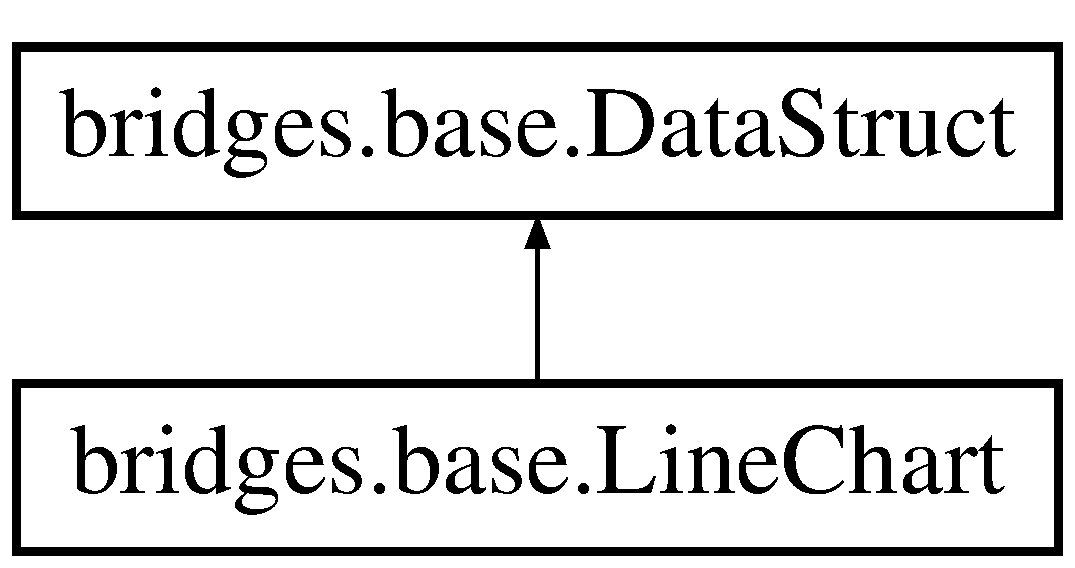
\includegraphics[height=2.000000cm]{classbridges_1_1base_1_1_line_chart}
\end{center}
\end{figure}


\subsection{Detailed Description}
Show series of data or functions using a line chart. 

Line charts (\href{https://en.wikipedia.org/wiki/Line_chart}{\tt https\+://en.\+wikipedia.\+org/wiki/\+Line\+\_\+chart}) are used to represent graphically functions such as f(x) = 3$\ast$x+1, or data such as temperature of a liquid on a stove as time passes. A individual function or a set of data are called \char`\"{}series\char`\"{}.

A series is represented by two arrays xdata and ydata such that there is a point at (xdata\mbox{[}0\mbox{]}, ydata\mbox{[}0\mbox{]}), an other at (xdata\mbox{[}1\mbox{]}, ydata\mbox{[}1\mbox{]}), ... One can add a series by passing the two arrays using \hyperlink{classbridges_1_1base_1_1_line_chart_a586e9953b13e51ab9e592acfb034887b}{set\+Data\+Series()} or add the arrays individually using \hyperlink{classbridges_1_1base_1_1_line_chart_a2918179283e8280d47abb43df3c59195}{set\+X\+Data()} and \hyperlink{classbridges_1_1base_1_1_line_chart_a3076dc99debb599529169de40815aba2}{set\+Y\+Data()}.

The different series have a label associated with them by default which can be disabled (see \hyperlink{classbridges_1_1base_1_1_line_chart_adae74cfb09585727a96cf74ddf74d098}{toggle\+Series\+Label()}).

The data is typically shown with axes that use a linear scale. However, the scale can be changed to logarithmic for each axis individually (see \hyperlink{classbridges_1_1base_1_1_line_chart_ad3e5e54c382ac605a81b6b61c250ad16}{toggle\+Logarithmic\+X()} and toggle\+Logarithmic()).

The \hyperlink{classbridges_1_1base_1_1_line_chart}{Line\+Chart} can have a title (see \hyperlink{classbridges_1_1base_1_1_line_chart_aedc5f75b158298b755ba0c31bcf84138}{get\+Title()} and \hyperlink{classbridges_1_1base_1_1_line_chart_a893519da804666988c49b918c87da2a2}{set\+Title()}) and a subtitle (see \hyperlink{classbridges_1_1base_1_1_line_chart_ad24bfdd49194f8e152fdb80e039762ad}{set\+Sub\+Title()} and \hyperlink{classbridges_1_1base_1_1_line_chart_a102006e90f2a226886538db0eeda6b08}{get\+Sub\+Title()}). \subsection*{Public Member Functions}
\begin{DoxyCompactItemize}
\item 
\hyperlink{classbridges_1_1base_1_1_line_chart_ae864fe5ae85e80ae2f035471fb216e68}{Line\+Chart} ()
\item 
String \hyperlink{classbridges_1_1base_1_1_line_chart_ae5d7ebffc6f29256f6fff368ef9a6c84}{get\+Data\+Struct\+Type} ()
\item 
void \hyperlink{classbridges_1_1base_1_1_line_chart_a095d16c1544cf373b8d2bf68ca864bd9}{toggle\+Mouse\+Track} (boolean val)
\begin{DoxyCompactList}\small\item\em Enables or disables mouse tracking. \end{DoxyCompactList}\item 
void \hyperlink{classbridges_1_1base_1_1_line_chart_adae74cfb09585727a96cf74ddf74d098}{toggle\+Series\+Label} (boolean val)
\begin{DoxyCompactList}\small\item\em Enables or disables series labels. \end{DoxyCompactList}\item 
void \hyperlink{classbridges_1_1base_1_1_line_chart_ad3e5e54c382ac605a81b6b61c250ad16}{toggle\+LogarithmicX} (boolean val)
\begin{DoxyCompactList}\small\item\em Change the X-\/axis scale to logarithmic. \end{DoxyCompactList}\item 
void \hyperlink{classbridges_1_1base_1_1_line_chart_a7946f217a7b3567ee1a1bd8266ed43ca}{toggle\+LogarithmicY} (boolean val)
\begin{DoxyCompactList}\small\item\em Change the Y-\/axis scale to logarithmic. \end{DoxyCompactList}\item 
void \hyperlink{classbridges_1_1base_1_1_line_chart_a893519da804666988c49b918c87da2a2}{set\+Title} (String t)
\begin{DoxyCompactList}\small\item\em Title of the plot. \end{DoxyCompactList}\item 
String \hyperlink{classbridges_1_1base_1_1_line_chart_aedc5f75b158298b755ba0c31bcf84138}{get\+Title} ()
\begin{DoxyCompactList}\small\item\em Title of the plot. \end{DoxyCompactList}\item 
void \hyperlink{classbridges_1_1base_1_1_line_chart_ad24bfdd49194f8e152fdb80e039762ad}{set\+Sub\+Title} (String s)
\begin{DoxyCompactList}\small\item\em Subtitle of the plot. \end{DoxyCompactList}\item 
String \hyperlink{classbridges_1_1base_1_1_line_chart_a102006e90f2a226886538db0eeda6b08}{get\+Sub\+Title} ()
\begin{DoxyCompactList}\small\item\em Subtitle of the plot. \end{DoxyCompactList}\item 
void \hyperlink{classbridges_1_1base_1_1_line_chart_adddccbe77ebd2590f426fab9c8227457}{set\+Y\+Label} (String yaxis\+Name)
\begin{DoxyCompactList}\small\item\em Change the label for the Y-\/axis. \end{DoxyCompactList}\item 
String \hyperlink{classbridges_1_1base_1_1_line_chart_ad3ae17da720b1f89406ab742379ddfd6}{get\+Y\+Label} ()
\begin{DoxyCompactList}\small\item\em Returns the label for the Y-\/axis. \end{DoxyCompactList}\item 
void \hyperlink{classbridges_1_1base_1_1_line_chart_ab402a1134bb79919860368a234f62ea2}{set\+X\+Label} (String xaxis\+Name)
\begin{DoxyCompactList}\small\item\em Change the label for the X-\/axis. \end{DoxyCompactList}\item 
String \hyperlink{classbridges_1_1base_1_1_line_chart_a0885f5c62f950d96397b1704da6e2798}{get\+X\+Label} ()
\begin{DoxyCompactList}\small\item\em Returns the label for the Y-\/axis. \end{DoxyCompactList}\item 
void \hyperlink{classbridges_1_1base_1_1_line_chart_a586e9953b13e51ab9e592acfb034887b}{set\+Data\+Series} (String series\+Name, double\mbox{[}$\,$\mbox{]} xdata, double\mbox{[}$\,$\mbox{]} ydata)
\begin{DoxyCompactList}\small\item\em Add a series (or update it) \end{DoxyCompactList}\item 
void \hyperlink{classbridges_1_1base_1_1_line_chart_ab3b577798d421da8d8519d73dcf7ceaf}{set\+Data\+Series} (String series\+Name, Array\+List$<$ Double $>$ xdata, Array\+List$<$ Double $>$ ydata)
\begin{DoxyCompactList}\small\item\em Add a series (or update it) \end{DoxyCompactList}\item 
void \hyperlink{classbridges_1_1base_1_1_line_chart_ac650a150cfbf2e572a5ccdb5d25cb00b}{set\+Data\+Series} (String series\+Name, double\mbox{[}$\,$\mbox{]} xdata, Array\+List$<$ Double $>$ ydata)
\begin{DoxyCompactList}\small\item\em Add a series (or update it) \end{DoxyCompactList}\item 
void \hyperlink{classbridges_1_1base_1_1_line_chart_a38eb16930491bc047a5343dd73052219}{set\+Data\+Series} (String series\+Name, Array\+List$<$ Double $>$ xdata, double\mbox{[}$\,$\mbox{]} ydata)
\begin{DoxyCompactList}\small\item\em Add a series (or update it) \end{DoxyCompactList}\item 
void \hyperlink{classbridges_1_1base_1_1_line_chart_a2918179283e8280d47abb43df3c59195}{set\+X\+Data} (String series, double\mbox{[}$\,$\mbox{]} xdata)
\begin{DoxyCompactList}\small\item\em Changes the X data for a series. \end{DoxyCompactList}\item 
void \hyperlink{classbridges_1_1base_1_1_line_chart_a2f141ec46fdafd92fb0d86900a2de46a}{set\+X\+Data} (String series, Array\+List$<$ Double $>$ xdata)
\begin{DoxyCompactList}\small\item\em Changes the X data for a series. \end{DoxyCompactList}\item 
double \mbox{[}$\,$\mbox{]} \hyperlink{classbridges_1_1base_1_1_line_chart_a34ef6ace0633d287a78d0e224f38f2ed}{get\+X\+Data} (String series)
\begin{DoxyCompactList}\small\item\em Returns the X data for a series. \end{DoxyCompactList}\item 
void \hyperlink{classbridges_1_1base_1_1_line_chart_a3076dc99debb599529169de40815aba2}{set\+Y\+Data} (String series, Array\+List$<$ Double $>$ ydata)
\begin{DoxyCompactList}\small\item\em Changes the Y data for a series. \end{DoxyCompactList}\item 
void \hyperlink{classbridges_1_1base_1_1_line_chart_aa8094fad197ae35d93f9feab5de91f59}{set\+Y\+Data} (String series, double\mbox{[}$\,$\mbox{]} ydata)
\begin{DoxyCompactList}\small\item\em Changes the Y data for a series. \end{DoxyCompactList}\item 
double \mbox{[}$\,$\mbox{]} \hyperlink{classbridges_1_1base_1_1_line_chart_a2bf257f45c1056808b41581af1f83645}{get\+Y\+Data} (String series)
\begin{DoxyCompactList}\small\item\em Returns the Y data for a series. \end{DoxyCompactList}\item 
String \hyperlink{classbridges_1_1base_1_1_line_chart_a1d481880dc94fc8c2dfdcf64d2de2a3b}{get\+Data\+Structure\+Representation} ()
\end{DoxyCompactItemize}
\subsection*{Additional Inherited Members}


\subsection{Constructor \& Destructor Documentation}
\mbox{\Hypertarget{classbridges_1_1base_1_1_line_chart_ae864fe5ae85e80ae2f035471fb216e68}\label{classbridges_1_1base_1_1_line_chart_ae864fe5ae85e80ae2f035471fb216e68}} 
\index{bridges\+::base\+::\+Line\+Chart@{bridges\+::base\+::\+Line\+Chart}!Line\+Chart@{Line\+Chart}}
\index{Line\+Chart@{Line\+Chart}!bridges\+::base\+::\+Line\+Chart@{bridges\+::base\+::\+Line\+Chart}}
\subsubsection{\texorpdfstring{Line\+Chart()}{LineChart()}}
{\footnotesize\ttfamily bridges.\+base.\+Line\+Chart.\+Line\+Chart (\begin{DoxyParamCaption}{ }\end{DoxyParamCaption})}



\subsection{Member Function Documentation}
\mbox{\Hypertarget{classbridges_1_1base_1_1_line_chart_ae5d7ebffc6f29256f6fff368ef9a6c84}\label{classbridges_1_1base_1_1_line_chart_ae5d7ebffc6f29256f6fff368ef9a6c84}} 
\index{bridges\+::base\+::\+Line\+Chart@{bridges\+::base\+::\+Line\+Chart}!get\+Data\+Struct\+Type@{get\+Data\+Struct\+Type}}
\index{get\+Data\+Struct\+Type@{get\+Data\+Struct\+Type}!bridges\+::base\+::\+Line\+Chart@{bridges\+::base\+::\+Line\+Chart}}
\subsubsection{\texorpdfstring{get\+Data\+Struct\+Type()}{getDataStructType()}}
{\footnotesize\ttfamily String bridges.\+base.\+Line\+Chart.\+get\+Data\+Struct\+Type (\begin{DoxyParamCaption}{ }\end{DoxyParamCaption})}

\mbox{\Hypertarget{classbridges_1_1base_1_1_line_chart_a1d481880dc94fc8c2dfdcf64d2de2a3b}\label{classbridges_1_1base_1_1_line_chart_a1d481880dc94fc8c2dfdcf64d2de2a3b}} 
\index{bridges\+::base\+::\+Line\+Chart@{bridges\+::base\+::\+Line\+Chart}!get\+Data\+Structure\+Representation@{get\+Data\+Structure\+Representation}}
\index{get\+Data\+Structure\+Representation@{get\+Data\+Structure\+Representation}!bridges\+::base\+::\+Line\+Chart@{bridges\+::base\+::\+Line\+Chart}}
\subsubsection{\texorpdfstring{get\+Data\+Structure\+Representation()}{getDataStructureRepresentation()}}
{\footnotesize\ttfamily String bridges.\+base.\+Line\+Chart.\+get\+Data\+Structure\+Representation (\begin{DoxyParamCaption}{ }\end{DoxyParamCaption})}

\mbox{\Hypertarget{classbridges_1_1base_1_1_line_chart_a102006e90f2a226886538db0eeda6b08}\label{classbridges_1_1base_1_1_line_chart_a102006e90f2a226886538db0eeda6b08}} 
\index{bridges\+::base\+::\+Line\+Chart@{bridges\+::base\+::\+Line\+Chart}!get\+Sub\+Title@{get\+Sub\+Title}}
\index{get\+Sub\+Title@{get\+Sub\+Title}!bridges\+::base\+::\+Line\+Chart@{bridges\+::base\+::\+Line\+Chart}}
\subsubsection{\texorpdfstring{get\+Sub\+Title()}{getSubTitle()}}
{\footnotesize\ttfamily String bridges.\+base.\+Line\+Chart.\+get\+Sub\+Title (\begin{DoxyParamCaption}{ }\end{DoxyParamCaption})}



Subtitle of the plot. 

\begin{DoxyReturn}{Returns}
the subtitle to be shown 
\end{DoxyReturn}
\mbox{\Hypertarget{classbridges_1_1base_1_1_line_chart_aedc5f75b158298b755ba0c31bcf84138}\label{classbridges_1_1base_1_1_line_chart_aedc5f75b158298b755ba0c31bcf84138}} 
\index{bridges\+::base\+::\+Line\+Chart@{bridges\+::base\+::\+Line\+Chart}!get\+Title@{get\+Title}}
\index{get\+Title@{get\+Title}!bridges\+::base\+::\+Line\+Chart@{bridges\+::base\+::\+Line\+Chart}}
\subsubsection{\texorpdfstring{get\+Title()}{getTitle()}}
{\footnotesize\ttfamily String bridges.\+base.\+Line\+Chart.\+get\+Title (\begin{DoxyParamCaption}{ }\end{DoxyParamCaption})}



Title of the plot. 

\begin{DoxyReturn}{Returns}
the title to be shown 
\end{DoxyReturn}
\mbox{\Hypertarget{classbridges_1_1base_1_1_line_chart_a34ef6ace0633d287a78d0e224f38f2ed}\label{classbridges_1_1base_1_1_line_chart_a34ef6ace0633d287a78d0e224f38f2ed}} 
\index{bridges\+::base\+::\+Line\+Chart@{bridges\+::base\+::\+Line\+Chart}!get\+X\+Data@{get\+X\+Data}}
\index{get\+X\+Data@{get\+X\+Data}!bridges\+::base\+::\+Line\+Chart@{bridges\+::base\+::\+Line\+Chart}}
\subsubsection{\texorpdfstring{get\+X\+Data()}{getXData()}}
{\footnotesize\ttfamily double \mbox{[}$\,$\mbox{]} bridges.\+base.\+Line\+Chart.\+get\+X\+Data (\begin{DoxyParamCaption}\item[{String}]{series }\end{DoxyParamCaption})}



Returns the X data for a series. 


\begin{DoxyParams}{Parameters}
{\em series} & indicate the series to get \\
\hline
\end{DoxyParams}
\begin{DoxyReturn}{Returns}
the X data of series or null if the series is not in there 
\end{DoxyReturn}
\mbox{\Hypertarget{classbridges_1_1base_1_1_line_chart_a0885f5c62f950d96397b1704da6e2798}\label{classbridges_1_1base_1_1_line_chart_a0885f5c62f950d96397b1704da6e2798}} 
\index{bridges\+::base\+::\+Line\+Chart@{bridges\+::base\+::\+Line\+Chart}!get\+X\+Label@{get\+X\+Label}}
\index{get\+X\+Label@{get\+X\+Label}!bridges\+::base\+::\+Line\+Chart@{bridges\+::base\+::\+Line\+Chart}}
\subsubsection{\texorpdfstring{get\+X\+Label()}{getXLabel()}}
{\footnotesize\ttfamily String bridges.\+base.\+Line\+Chart.\+get\+X\+Label (\begin{DoxyParamCaption}{ }\end{DoxyParamCaption})}



Returns the label for the Y-\/axis. 

\begin{DoxyReturn}{Returns}
label shown for the Y-\/axis 
\end{DoxyReturn}
\mbox{\Hypertarget{classbridges_1_1base_1_1_line_chart_a2bf257f45c1056808b41581af1f83645}\label{classbridges_1_1base_1_1_line_chart_a2bf257f45c1056808b41581af1f83645}} 
\index{bridges\+::base\+::\+Line\+Chart@{bridges\+::base\+::\+Line\+Chart}!get\+Y\+Data@{get\+Y\+Data}}
\index{get\+Y\+Data@{get\+Y\+Data}!bridges\+::base\+::\+Line\+Chart@{bridges\+::base\+::\+Line\+Chart}}
\subsubsection{\texorpdfstring{get\+Y\+Data()}{getYData()}}
{\footnotesize\ttfamily double \mbox{[}$\,$\mbox{]} bridges.\+base.\+Line\+Chart.\+get\+Y\+Data (\begin{DoxyParamCaption}\item[{String}]{series }\end{DoxyParamCaption})}



Returns the Y data for a series. 


\begin{DoxyParams}{Parameters}
{\em series} & indicate the series to get \\
\hline
\end{DoxyParams}
\begin{DoxyReturn}{Returns}
the Y data of series or null if the data is not in there 
\end{DoxyReturn}
\mbox{\Hypertarget{classbridges_1_1base_1_1_line_chart_ad3ae17da720b1f89406ab742379ddfd6}\label{classbridges_1_1base_1_1_line_chart_ad3ae17da720b1f89406ab742379ddfd6}} 
\index{bridges\+::base\+::\+Line\+Chart@{bridges\+::base\+::\+Line\+Chart}!get\+Y\+Label@{get\+Y\+Label}}
\index{get\+Y\+Label@{get\+Y\+Label}!bridges\+::base\+::\+Line\+Chart@{bridges\+::base\+::\+Line\+Chart}}
\subsubsection{\texorpdfstring{get\+Y\+Label()}{getYLabel()}}
{\footnotesize\ttfamily String bridges.\+base.\+Line\+Chart.\+get\+Y\+Label (\begin{DoxyParamCaption}{ }\end{DoxyParamCaption})}



Returns the label for the Y-\/axis. 

\begin{DoxyReturn}{Returns}
label shown for the Y-\/axis 
\end{DoxyReturn}
\mbox{\Hypertarget{classbridges_1_1base_1_1_line_chart_a586e9953b13e51ab9e592acfb034887b}\label{classbridges_1_1base_1_1_line_chart_a586e9953b13e51ab9e592acfb034887b}} 
\index{bridges\+::base\+::\+Line\+Chart@{bridges\+::base\+::\+Line\+Chart}!set\+Data\+Series@{set\+Data\+Series}}
\index{set\+Data\+Series@{set\+Data\+Series}!bridges\+::base\+::\+Line\+Chart@{bridges\+::base\+::\+Line\+Chart}}
\subsubsection{\texorpdfstring{set\+Data\+Series()}{setDataSeries()}\hspace{0.1cm}{\footnotesize\ttfamily [1/4]}}
{\footnotesize\ttfamily void bridges.\+base.\+Line\+Chart.\+set\+Data\+Series (\begin{DoxyParamCaption}\item[{String}]{series\+Name,  }\item[{double \mbox{[}$\,$\mbox{]}}]{xdata,  }\item[{double \mbox{[}$\,$\mbox{]}}]{ydata }\end{DoxyParamCaption})}



Add a series (or update it) 


\begin{DoxyParams}{Parameters}
{\em series\+Name} & indicates the series to add (or change) \\
\hline
{\em xdata} & the X data in the series \\
\hline
{\em ydata} & the Y data in the series \\
\hline
\end{DoxyParams}
\mbox{\Hypertarget{classbridges_1_1base_1_1_line_chart_ab3b577798d421da8d8519d73dcf7ceaf}\label{classbridges_1_1base_1_1_line_chart_ab3b577798d421da8d8519d73dcf7ceaf}} 
\index{bridges\+::base\+::\+Line\+Chart@{bridges\+::base\+::\+Line\+Chart}!set\+Data\+Series@{set\+Data\+Series}}
\index{set\+Data\+Series@{set\+Data\+Series}!bridges\+::base\+::\+Line\+Chart@{bridges\+::base\+::\+Line\+Chart}}
\subsubsection{\texorpdfstring{set\+Data\+Series()}{setDataSeries()}\hspace{0.1cm}{\footnotesize\ttfamily [2/4]}}
{\footnotesize\ttfamily void bridges.\+base.\+Line\+Chart.\+set\+Data\+Series (\begin{DoxyParamCaption}\item[{String}]{series\+Name,  }\item[{Array\+List$<$ Double $>$}]{xdata,  }\item[{Array\+List$<$ Double $>$}]{ydata }\end{DoxyParamCaption})}



Add a series (or update it) 


\begin{DoxyParams}{Parameters}
{\em series\+Name} & indicates the series to add (or change) \\
\hline
{\em xdata} & the X data in the series \\
\hline
{\em ydata} & the Y data in the series \\
\hline
\end{DoxyParams}
\mbox{\Hypertarget{classbridges_1_1base_1_1_line_chart_ac650a150cfbf2e572a5ccdb5d25cb00b}\label{classbridges_1_1base_1_1_line_chart_ac650a150cfbf2e572a5ccdb5d25cb00b}} 
\index{bridges\+::base\+::\+Line\+Chart@{bridges\+::base\+::\+Line\+Chart}!set\+Data\+Series@{set\+Data\+Series}}
\index{set\+Data\+Series@{set\+Data\+Series}!bridges\+::base\+::\+Line\+Chart@{bridges\+::base\+::\+Line\+Chart}}
\subsubsection{\texorpdfstring{set\+Data\+Series()}{setDataSeries()}\hspace{0.1cm}{\footnotesize\ttfamily [3/4]}}
{\footnotesize\ttfamily void bridges.\+base.\+Line\+Chart.\+set\+Data\+Series (\begin{DoxyParamCaption}\item[{String}]{series\+Name,  }\item[{double \mbox{[}$\,$\mbox{]}}]{xdata,  }\item[{Array\+List$<$ Double $>$}]{ydata }\end{DoxyParamCaption})}



Add a series (or update it) 


\begin{DoxyParams}{Parameters}
{\em series\+Name} & indicates the series to add (or change) \\
\hline
{\em xdata} & the X data in the series \\
\hline
{\em ydata} & the Y data in the series \\
\hline
\end{DoxyParams}
\mbox{\Hypertarget{classbridges_1_1base_1_1_line_chart_a38eb16930491bc047a5343dd73052219}\label{classbridges_1_1base_1_1_line_chart_a38eb16930491bc047a5343dd73052219}} 
\index{bridges\+::base\+::\+Line\+Chart@{bridges\+::base\+::\+Line\+Chart}!set\+Data\+Series@{set\+Data\+Series}}
\index{set\+Data\+Series@{set\+Data\+Series}!bridges\+::base\+::\+Line\+Chart@{bridges\+::base\+::\+Line\+Chart}}
\subsubsection{\texorpdfstring{set\+Data\+Series()}{setDataSeries()}\hspace{0.1cm}{\footnotesize\ttfamily [4/4]}}
{\footnotesize\ttfamily void bridges.\+base.\+Line\+Chart.\+set\+Data\+Series (\begin{DoxyParamCaption}\item[{String}]{series\+Name,  }\item[{Array\+List$<$ Double $>$}]{xdata,  }\item[{double \mbox{[}$\,$\mbox{]}}]{ydata }\end{DoxyParamCaption})}



Add a series (or update it) 


\begin{DoxyParams}{Parameters}
{\em series\+Name} & indicates the series to add (or change) \\
\hline
{\em xdata} & the X data in the series \\
\hline
{\em ydata} & the Y data in the series \\
\hline
\end{DoxyParams}
\mbox{\Hypertarget{classbridges_1_1base_1_1_line_chart_ad24bfdd49194f8e152fdb80e039762ad}\label{classbridges_1_1base_1_1_line_chart_ad24bfdd49194f8e152fdb80e039762ad}} 
\index{bridges\+::base\+::\+Line\+Chart@{bridges\+::base\+::\+Line\+Chart}!set\+Sub\+Title@{set\+Sub\+Title}}
\index{set\+Sub\+Title@{set\+Sub\+Title}!bridges\+::base\+::\+Line\+Chart@{bridges\+::base\+::\+Line\+Chart}}
\subsubsection{\texorpdfstring{set\+Sub\+Title()}{setSubTitle()}}
{\footnotesize\ttfamily void bridges.\+base.\+Line\+Chart.\+set\+Sub\+Title (\begin{DoxyParamCaption}\item[{String}]{s }\end{DoxyParamCaption})}



Subtitle of the plot. 


\begin{DoxyParams}{Parameters}
{\em s} & the subtitle to be shown \\
\hline
\end{DoxyParams}
\mbox{\Hypertarget{classbridges_1_1base_1_1_line_chart_a893519da804666988c49b918c87da2a2}\label{classbridges_1_1base_1_1_line_chart_a893519da804666988c49b918c87da2a2}} 
\index{bridges\+::base\+::\+Line\+Chart@{bridges\+::base\+::\+Line\+Chart}!set\+Title@{set\+Title}}
\index{set\+Title@{set\+Title}!bridges\+::base\+::\+Line\+Chart@{bridges\+::base\+::\+Line\+Chart}}
\subsubsection{\texorpdfstring{set\+Title()}{setTitle()}}
{\footnotesize\ttfamily void bridges.\+base.\+Line\+Chart.\+set\+Title (\begin{DoxyParamCaption}\item[{String}]{t }\end{DoxyParamCaption})}



Title of the plot. 


\begin{DoxyParams}{Parameters}
{\em t} & the title to be shown \\
\hline
\end{DoxyParams}
\mbox{\Hypertarget{classbridges_1_1base_1_1_line_chart_a2918179283e8280d47abb43df3c59195}\label{classbridges_1_1base_1_1_line_chart_a2918179283e8280d47abb43df3c59195}} 
\index{bridges\+::base\+::\+Line\+Chart@{bridges\+::base\+::\+Line\+Chart}!set\+X\+Data@{set\+X\+Data}}
\index{set\+X\+Data@{set\+X\+Data}!bridges\+::base\+::\+Line\+Chart@{bridges\+::base\+::\+Line\+Chart}}
\subsubsection{\texorpdfstring{set\+X\+Data()}{setXData()}\hspace{0.1cm}{\footnotesize\ttfamily [1/2]}}
{\footnotesize\ttfamily void bridges.\+base.\+Line\+Chart.\+set\+X\+Data (\begin{DoxyParamCaption}\item[{String}]{series,  }\item[{double \mbox{[}$\,$\mbox{]}}]{xdata }\end{DoxyParamCaption})}



Changes the X data for a series. 


\begin{DoxyParams}{Parameters}
{\em series} & indicates the series to get \\
\hline
{\em xdata} & the X data in the series \\
\hline
\end{DoxyParams}
\mbox{\Hypertarget{classbridges_1_1base_1_1_line_chart_a2f141ec46fdafd92fb0d86900a2de46a}\label{classbridges_1_1base_1_1_line_chart_a2f141ec46fdafd92fb0d86900a2de46a}} 
\index{bridges\+::base\+::\+Line\+Chart@{bridges\+::base\+::\+Line\+Chart}!set\+X\+Data@{set\+X\+Data}}
\index{set\+X\+Data@{set\+X\+Data}!bridges\+::base\+::\+Line\+Chart@{bridges\+::base\+::\+Line\+Chart}}
\subsubsection{\texorpdfstring{set\+X\+Data()}{setXData()}\hspace{0.1cm}{\footnotesize\ttfamily [2/2]}}
{\footnotesize\ttfamily void bridges.\+base.\+Line\+Chart.\+set\+X\+Data (\begin{DoxyParamCaption}\item[{String}]{series,  }\item[{Array\+List$<$ Double $>$}]{xdata }\end{DoxyParamCaption})}



Changes the X data for a series. 


\begin{DoxyParams}{Parameters}
{\em series} & indicates the series to get \\
\hline
{\em xdata} & the X data in the series \\
\hline
\end{DoxyParams}
\mbox{\Hypertarget{classbridges_1_1base_1_1_line_chart_ab402a1134bb79919860368a234f62ea2}\label{classbridges_1_1base_1_1_line_chart_ab402a1134bb79919860368a234f62ea2}} 
\index{bridges\+::base\+::\+Line\+Chart@{bridges\+::base\+::\+Line\+Chart}!set\+X\+Label@{set\+X\+Label}}
\index{set\+X\+Label@{set\+X\+Label}!bridges\+::base\+::\+Line\+Chart@{bridges\+::base\+::\+Line\+Chart}}
\subsubsection{\texorpdfstring{set\+X\+Label()}{setXLabel()}}
{\footnotesize\ttfamily void bridges.\+base.\+Line\+Chart.\+set\+X\+Label (\begin{DoxyParamCaption}\item[{String}]{xaxis\+Name }\end{DoxyParamCaption})}



Change the label for the X-\/axis. 


\begin{DoxyParams}{Parameters}
{\em xaxis\+Name} & label to use for the X-\/axis \\
\hline
\end{DoxyParams}
\mbox{\Hypertarget{classbridges_1_1base_1_1_line_chart_a3076dc99debb599529169de40815aba2}\label{classbridges_1_1base_1_1_line_chart_a3076dc99debb599529169de40815aba2}} 
\index{bridges\+::base\+::\+Line\+Chart@{bridges\+::base\+::\+Line\+Chart}!set\+Y\+Data@{set\+Y\+Data}}
\index{set\+Y\+Data@{set\+Y\+Data}!bridges\+::base\+::\+Line\+Chart@{bridges\+::base\+::\+Line\+Chart}}
\subsubsection{\texorpdfstring{set\+Y\+Data()}{setYData()}\hspace{0.1cm}{\footnotesize\ttfamily [1/2]}}
{\footnotesize\ttfamily void bridges.\+base.\+Line\+Chart.\+set\+Y\+Data (\begin{DoxyParamCaption}\item[{String}]{series,  }\item[{Array\+List$<$ Double $>$}]{ydata }\end{DoxyParamCaption})}



Changes the Y data for a series. 


\begin{DoxyParams}{Parameters}
{\em series} & indicates the series to get \\
\hline
{\em ydata} & the Y data in the series \\
\hline
\end{DoxyParams}
\mbox{\Hypertarget{classbridges_1_1base_1_1_line_chart_aa8094fad197ae35d93f9feab5de91f59}\label{classbridges_1_1base_1_1_line_chart_aa8094fad197ae35d93f9feab5de91f59}} 
\index{bridges\+::base\+::\+Line\+Chart@{bridges\+::base\+::\+Line\+Chart}!set\+Y\+Data@{set\+Y\+Data}}
\index{set\+Y\+Data@{set\+Y\+Data}!bridges\+::base\+::\+Line\+Chart@{bridges\+::base\+::\+Line\+Chart}}
\subsubsection{\texorpdfstring{set\+Y\+Data()}{setYData()}\hspace{0.1cm}{\footnotesize\ttfamily [2/2]}}
{\footnotesize\ttfamily void bridges.\+base.\+Line\+Chart.\+set\+Y\+Data (\begin{DoxyParamCaption}\item[{String}]{series,  }\item[{double \mbox{[}$\,$\mbox{]}}]{ydata }\end{DoxyParamCaption})}



Changes the Y data for a series. 


\begin{DoxyParams}{Parameters}
{\em series} & indicates the series to get \\
\hline
{\em ydata} & the Y data in the series \\
\hline
\end{DoxyParams}
\mbox{\Hypertarget{classbridges_1_1base_1_1_line_chart_adddccbe77ebd2590f426fab9c8227457}\label{classbridges_1_1base_1_1_line_chart_adddccbe77ebd2590f426fab9c8227457}} 
\index{bridges\+::base\+::\+Line\+Chart@{bridges\+::base\+::\+Line\+Chart}!set\+Y\+Label@{set\+Y\+Label}}
\index{set\+Y\+Label@{set\+Y\+Label}!bridges\+::base\+::\+Line\+Chart@{bridges\+::base\+::\+Line\+Chart}}
\subsubsection{\texorpdfstring{set\+Y\+Label()}{setYLabel()}}
{\footnotesize\ttfamily void bridges.\+base.\+Line\+Chart.\+set\+Y\+Label (\begin{DoxyParamCaption}\item[{String}]{yaxis\+Name }\end{DoxyParamCaption})}



Change the label for the Y-\/axis. 


\begin{DoxyParams}{Parameters}
{\em yaxis\+Name} & label to show for the Y-\/axis \\
\hline
\end{DoxyParams}
\mbox{\Hypertarget{classbridges_1_1base_1_1_line_chart_ad3e5e54c382ac605a81b6b61c250ad16}\label{classbridges_1_1base_1_1_line_chart_ad3e5e54c382ac605a81b6b61c250ad16}} 
\index{bridges\+::base\+::\+Line\+Chart@{bridges\+::base\+::\+Line\+Chart}!toggle\+LogarithmicX@{toggle\+LogarithmicX}}
\index{toggle\+LogarithmicX@{toggle\+LogarithmicX}!bridges\+::base\+::\+Line\+Chart@{bridges\+::base\+::\+Line\+Chart}}
\subsubsection{\texorpdfstring{toggle\+Logarithmic\+X()}{toggleLogarithmicX()}}
{\footnotesize\ttfamily void bridges.\+base.\+Line\+Chart.\+toggle\+LogarithmicX (\begin{DoxyParamCaption}\item[{boolean}]{val }\end{DoxyParamCaption})}



Change the X-\/axis scale to logarithmic. 

When enabled, the X-\/axis scale becomes logarithmic (as opposed to linear).


\begin{DoxyParams}{Parameters}
{\em val} & Should the X-\/axis use a logarithmic scale? \\
\hline
\end{DoxyParams}
\mbox{\Hypertarget{classbridges_1_1base_1_1_line_chart_a7946f217a7b3567ee1a1bd8266ed43ca}\label{classbridges_1_1base_1_1_line_chart_a7946f217a7b3567ee1a1bd8266ed43ca}} 
\index{bridges\+::base\+::\+Line\+Chart@{bridges\+::base\+::\+Line\+Chart}!toggle\+LogarithmicY@{toggle\+LogarithmicY}}
\index{toggle\+LogarithmicY@{toggle\+LogarithmicY}!bridges\+::base\+::\+Line\+Chart@{bridges\+::base\+::\+Line\+Chart}}
\subsubsection{\texorpdfstring{toggle\+Logarithmic\+Y()}{toggleLogarithmicY()}}
{\footnotesize\ttfamily void bridges.\+base.\+Line\+Chart.\+toggle\+LogarithmicY (\begin{DoxyParamCaption}\item[{boolean}]{val }\end{DoxyParamCaption})}



Change the Y-\/axis scale to logarithmic. 

When enabled, the Y-\/axis scale becomes logarithmic (as opposed to linear).


\begin{DoxyParams}{Parameters}
{\em val} & Should the Y-\/axis use a logarithmic scale? \\
\hline
\end{DoxyParams}
\mbox{\Hypertarget{classbridges_1_1base_1_1_line_chart_a095d16c1544cf373b8d2bf68ca864bd9}\label{classbridges_1_1base_1_1_line_chart_a095d16c1544cf373b8d2bf68ca864bd9}} 
\index{bridges\+::base\+::\+Line\+Chart@{bridges\+::base\+::\+Line\+Chart}!toggle\+Mouse\+Track@{toggle\+Mouse\+Track}}
\index{toggle\+Mouse\+Track@{toggle\+Mouse\+Track}!bridges\+::base\+::\+Line\+Chart@{bridges\+::base\+::\+Line\+Chart}}
\subsubsection{\texorpdfstring{toggle\+Mouse\+Track()}{toggleMouseTrack()}}
{\footnotesize\ttfamily void bridges.\+base.\+Line\+Chart.\+toggle\+Mouse\+Track (\begin{DoxyParamCaption}\item[{boolean}]{val }\end{DoxyParamCaption})}



Enables or disables mouse tracking. 

Mouse tracking show the value of a data point when the mouse hovers on a data point.


\begin{DoxyParams}{Parameters}
{\em val} & Should mouse tracking be activated or not. \\
\hline
\end{DoxyParams}
\mbox{\Hypertarget{classbridges_1_1base_1_1_line_chart_adae74cfb09585727a96cf74ddf74d098}\label{classbridges_1_1base_1_1_line_chart_adae74cfb09585727a96cf74ddf74d098}} 
\index{bridges\+::base\+::\+Line\+Chart@{bridges\+::base\+::\+Line\+Chart}!toggle\+Series\+Label@{toggle\+Series\+Label}}
\index{toggle\+Series\+Label@{toggle\+Series\+Label}!bridges\+::base\+::\+Line\+Chart@{bridges\+::base\+::\+Line\+Chart}}
\subsubsection{\texorpdfstring{toggle\+Series\+Label()}{toggleSeriesLabel()}}
{\footnotesize\ttfamily void bridges.\+base.\+Line\+Chart.\+toggle\+Series\+Label (\begin{DoxyParamCaption}\item[{boolean}]{val }\end{DoxyParamCaption})}



Enables or disables series labels. 

When enabled, the name of the series will be shown on the line chart.


\begin{DoxyParams}{Parameters}
{\em val} & Should series be labeled or not \\
\hline
\end{DoxyParams}


The documentation for this class was generated from the following file\+:\begin{DoxyCompactItemize}
\item 
/home/erik/work/bridges/bridges-\/java/src/main/java/bridges/base/\hyperlink{_line_chart_8java}{Line\+Chart.\+java}\end{DoxyCompactItemize}

\hypertarget{classbridges_1_1base_1_1_link_visualizer}{}\section{bridges.\+base.\+Link\+Visualizer Class Reference}
\label{classbridges_1_1base_1_1_link_visualizer}\index{bridges.\+base.\+Link\+Visualizer@{bridges.\+base.\+Link\+Visualizer}}


This class maintains the visual attributes of links that join Bridges elements.  


\subsection*{Public Member Functions}
\begin{DoxyCompactItemize}
\item 
\hyperlink{classbridges_1_1base_1_1_link_visualizer_a0b69f099fa264ae9097b0efe278c6a1b}{Link\+Visualizer} ()
\item 
void \hyperlink{classbridges_1_1base_1_1_link_visualizer_a702e9ca345d1a4a035baf2041f275849}{set\+Thickness} (double th)
\item 
double \hyperlink{classbridges_1_1base_1_1_link_visualizer_af1592d2a8664b00c1a51fdc0f8d1860a}{get\+Thickness} ()
\item 
void \hyperlink{classbridges_1_1base_1_1_link_visualizer_a21d5884d243cf5a08f9d544f5083a44c}{set\+Weight} (double wt)
\item 
double \hyperlink{classbridges_1_1base_1_1_link_visualizer_ac96d7fb118ae6c7e1bdd57c5e2c8639a}{get\+Weight} ()
\item 
void \hyperlink{classbridges_1_1base_1_1_link_visualizer_a92f306dbd73b961befa8ab4c0620a89e}{set\+Color} (String col\+\_\+name)
\item 
void \hyperlink{classbridges_1_1base_1_1_link_visualizer_a003905cfe33e1704555b2b3a1cf99bad}{set\+Color} (Integer r, Integer g, Integer b, Float a)  throws Invalid\+Value\+Exception 
\item 
\hyperlink{classbridges_1_1base_1_1_color}{Color} \hyperlink{classbridges_1_1base_1_1_link_visualizer_a3ed52d98ecab99c6d8dd136fba913b7d}{get\+Color} ()
\item 
void \hyperlink{classbridges_1_1base_1_1_link_visualizer_ac0d59614dbc65ed0a19c25c493a1deaa}{set\+Opacity} (float opacity)
\item 
float \hyperlink{classbridges_1_1base_1_1_link_visualizer_a07cdd435a54e4b612ad63614f2a27a4a}{get\+Opacity} ()
\item 
String \hyperlink{classbridges_1_1base_1_1_link_visualizer_ab64d9b7e2b99f7ebce80cbabfe4adf2a}{get\+Link\+Properties} ()
\end{DoxyCompactItemize}


\subsection{Detailed Description}
This class maintains the visual attributes of links that join Bridges elements. 

Visual properties include color, thickness, and opacity. Objects of this class are stored as part of the \hyperlink{classbridges_1_1base_1_1_element}{Element} class. Generally, a user will manipulate the \hyperlink{classbridges_1_1base_1_1_link_visualizer}{Link\+Visualizer} returned from the \hyperlink{classbridges_1_1base_1_1_element}{Element}\textquotesingle{}s get\+Link\+Visualizer(\+Element it) method (which it is the Bridges element this element is linked to), and then set attributes using its methods. Links are utilized in all types of linked lists, tree and graph structures.

Supported attribute values are as follows\+:

{\bfseries Supported Colors (by name)}\+: 

\char`\"{}red\char`\"{}, \char`\"{}green\char`\"{}, \char`\"{}blue\char`\"{},\char`\"{}yellow\char`\"{},\char`\"{}cyan\char`\"{},\char`\"{}magenta\char`\"{}, \char`\"{}white\char`\"{},, \char`\"{}black\char`\"{}, \char`\"{}orange\char`\"{}, \char`\"{}turquoise\char`\"{}, \char`\"{}maroon\char`\"{}, ~\newline
 \char`\"{}aquamarine\char`\"{}, \char`\"{}azure\char`\"{}, \char`\"{}beige\char`\"{}, \char`\"{}brown\char`\"{}, \char`\"{}tan\char`\"{}, \char`\"{}olive\char`\"{}, \char`\"{}chartreuse\char`\"{}, \char`\"{}khaki\char`\"{}, \char`\"{}bisque\char`\"{}, \char`\"{}coral\char`\"{}, ~\newline
 \char`\"{}pink\char`\"{}, \char`\"{}lavender\char`\"{}, \char`\"{}purple\char`\"{}, \char`\"{}gold\char`\"{} 

{\bfseries  \hyperlink{classbridges_1_1base_1_1_color}{Color} by R\+G\+BA Specification \+:} Range\+: 0-\/255 for each component 

{\bfseries  Thickness\+: } Range \+: 0.\+0-\/50.\+0

{\bfseries  Opacity\+: } Range (0.\+0-\/1.\+0) 

\begin{DoxyAuthor}{Author}
Mihai Mehedint, Kalpathi Subramanian
\end{DoxyAuthor}
\begin{DoxyDate}{Date}
6/22/16, 1/16/17, 5/17/17
\end{DoxyDate}
\begin{DoxySeeAlso}{See also}
Example Tutorial at ~\newline
 \href{http://bridgesuncc.github.io/Hello_World_Tutorials/SLL.html}{\tt http\+://bridgesuncc.\+github.\+io/\+Hello\+\_\+\+World\+\_\+\+Tutorials/\+S\+L\+L.\+html} 
\end{DoxySeeAlso}


\subsection{Constructor \& Destructor Documentation}
\hypertarget{classbridges_1_1base_1_1_link_visualizer_a0b69f099fa264ae9097b0efe278c6a1b}{}\label{classbridges_1_1base_1_1_link_visualizer_a0b69f099fa264ae9097b0efe278c6a1b} 
\index{bridges\+::base\+::\+Link\+Visualizer@{bridges\+::base\+::\+Link\+Visualizer}!Link\+Visualizer@{Link\+Visualizer}}
\index{Link\+Visualizer@{Link\+Visualizer}!bridges\+::base\+::\+Link\+Visualizer@{bridges\+::base\+::\+Link\+Visualizer}}
\subsubsection{\texorpdfstring{Link\+Visualizer()}{LinkVisualizer()}}
{\footnotesize\ttfamily bridges.\+base.\+Link\+Visualizer.\+Link\+Visualizer (\begin{DoxyParamCaption}{ }\end{DoxyParamCaption})}



\subsection{Member Function Documentation}
\hypertarget{classbridges_1_1base_1_1_link_visualizer_a3ed52d98ecab99c6d8dd136fba913b7d}{}\label{classbridges_1_1base_1_1_link_visualizer_a3ed52d98ecab99c6d8dd136fba913b7d} 
\index{bridges\+::base\+::\+Link\+Visualizer@{bridges\+::base\+::\+Link\+Visualizer}!get\+Color@{get\+Color}}
\index{get\+Color@{get\+Color}!bridges\+::base\+::\+Link\+Visualizer@{bridges\+::base\+::\+Link\+Visualizer}}
\subsubsection{\texorpdfstring{get\+Color()}{getColor()}}
{\footnotesize\ttfamily \hyperlink{classbridges_1_1base_1_1_color}{Color} bridges.\+base.\+Link\+Visualizer.\+get\+Color (\begin{DoxyParamCaption}{ }\end{DoxyParamCaption})}

Get the color of the link in the Bridges Visualization

\begin{DoxyReturn}{Returns}
the \hyperlink{classbridges_1_1base_1_1_color}{Color} object representing the color of the link 
\end{DoxyReturn}
\hypertarget{classbridges_1_1base_1_1_link_visualizer_ab64d9b7e2b99f7ebce80cbabfe4adf2a}{}\label{classbridges_1_1base_1_1_link_visualizer_ab64d9b7e2b99f7ebce80cbabfe4adf2a} 
\index{bridges\+::base\+::\+Link\+Visualizer@{bridges\+::base\+::\+Link\+Visualizer}!get\+Link\+Properties@{get\+Link\+Properties}}
\index{get\+Link\+Properties@{get\+Link\+Properties}!bridges\+::base\+::\+Link\+Visualizer@{bridges\+::base\+::\+Link\+Visualizer}}
\subsubsection{\texorpdfstring{get\+Link\+Properties()}{getLinkProperties()}}
{\footnotesize\ttfamily String bridges.\+base.\+Link\+Visualizer.\+get\+Link\+Properties (\begin{DoxyParamCaption}{ }\end{DoxyParamCaption})}

\hypertarget{classbridges_1_1base_1_1_link_visualizer_a07cdd435a54e4b612ad63614f2a27a4a}{}\label{classbridges_1_1base_1_1_link_visualizer_a07cdd435a54e4b612ad63614f2a27a4a} 
\index{bridges\+::base\+::\+Link\+Visualizer@{bridges\+::base\+::\+Link\+Visualizer}!get\+Opacity@{get\+Opacity}}
\index{get\+Opacity@{get\+Opacity}!bridges\+::base\+::\+Link\+Visualizer@{bridges\+::base\+::\+Link\+Visualizer}}
\subsubsection{\texorpdfstring{get\+Opacity()}{getOpacity()}}
{\footnotesize\ttfamily float bridges.\+base.\+Link\+Visualizer.\+get\+Opacity (\begin{DoxyParamCaption}{ }\end{DoxyParamCaption})}

Get the opacity of the link in the Bridges Visualization

\begin{DoxyReturn}{Returns}
the opacity value (in the range 0.\+0-\/1.\+0 
\end{DoxyReturn}
\hypertarget{classbridges_1_1base_1_1_link_visualizer_af1592d2a8664b00c1a51fdc0f8d1860a}{}\label{classbridges_1_1base_1_1_link_visualizer_af1592d2a8664b00c1a51fdc0f8d1860a} 
\index{bridges\+::base\+::\+Link\+Visualizer@{bridges\+::base\+::\+Link\+Visualizer}!get\+Thickness@{get\+Thickness}}
\index{get\+Thickness@{get\+Thickness}!bridges\+::base\+::\+Link\+Visualizer@{bridges\+::base\+::\+Link\+Visualizer}}
\subsubsection{\texorpdfstring{get\+Thickness()}{getThickness()}}
{\footnotesize\ttfamily double bridges.\+base.\+Link\+Visualizer.\+get\+Thickness (\begin{DoxyParamCaption}{ }\end{DoxyParamCaption})}

Get the thickness of the link in the Bridges Visualiation

\begin{DoxyReturn}{Returns}
the size in pixels of the \hyperlink{classbridges_1_1base_1_1_element}{Element} in the Bridges Visualization 
\end{DoxyReturn}
\hypertarget{classbridges_1_1base_1_1_link_visualizer_ac96d7fb118ae6c7e1bdd57c5e2c8639a}{}\label{classbridges_1_1base_1_1_link_visualizer_ac96d7fb118ae6c7e1bdd57c5e2c8639a} 
\index{bridges\+::base\+::\+Link\+Visualizer@{bridges\+::base\+::\+Link\+Visualizer}!get\+Weight@{get\+Weight}}
\index{get\+Weight@{get\+Weight}!bridges\+::base\+::\+Link\+Visualizer@{bridges\+::base\+::\+Link\+Visualizer}}
\subsubsection{\texorpdfstring{get\+Weight()}{getWeight()}}
{\footnotesize\ttfamily double bridges.\+base.\+Link\+Visualizer.\+get\+Weight (\begin{DoxyParamCaption}{ }\end{DoxyParamCaption})}

Get the weight of the link

\begin{DoxyReturn}{Returns}
the stored edge weight 
\end{DoxyReturn}
\hypertarget{classbridges_1_1base_1_1_link_visualizer_a92f306dbd73b961befa8ab4c0620a89e}{}\label{classbridges_1_1base_1_1_link_visualizer_a92f306dbd73b961befa8ab4c0620a89e} 
\index{bridges\+::base\+::\+Link\+Visualizer@{bridges\+::base\+::\+Link\+Visualizer}!set\+Color@{set\+Color}}
\index{set\+Color@{set\+Color}!bridges\+::base\+::\+Link\+Visualizer@{bridges\+::base\+::\+Link\+Visualizer}}
\subsubsection{\texorpdfstring{set\+Color()}{setColor()}\hspace{0.1cm}{\footnotesize\ttfamily [1/2]}}
{\footnotesize\ttfamily void bridges.\+base.\+Link\+Visualizer.\+set\+Color (\begin{DoxyParamCaption}\item[{String}]{col\+\_\+name }\end{DoxyParamCaption})}

Set the color of the link in the Bridges Visualization to \char`\"{}a\+Color\char`\"{}.


\begin{DoxyParams}{Parameters}
{\em col\+\_\+name} & the string reprsenting the color of the \hyperlink{classbridges_1_1base_1_1_element}{Element} in the Bridges Visualization; supported named colors are \char`\"{}red\char`\"{}, \char`\"{}green\char`\"{}, \char`\"{}blue\char`\"{}, \char`\"{}yellow\char`\"{}, \char`\"{}cyan\char`\"{}, \char`\"{}magenta\char`\"{}, \char`\"{}white\char`\"{}, \char`\"{}black\char`\"{}, \char`\"{}orange\char`\"{}, \char`\"{}turquoise\char`\"{}, \char`\"{}maroon\char`\"{}, \char`\"{}aquamarine\char`\"{}, \char`\"{}azure\char`\"{}, \char`\"{}beige\char`\"{}, \char`\"{}brown\char`\"{}, \char`\"{}tan\char`\"{}, \char`\"{}olive\char`\"{}, \char`\"{}chartreuse\char`\"{}, \char`\"{}khaki\char`\"{}, \char`\"{}bisque\char`\"{}, \char`\"{}coral\char`\"{}, \char`\"{}pink\char`\"{}, \char`\"{}lavender\char`\"{}, \char`\"{}purple\char`\"{}, \char`\"{}gold\char`\"{} \\
\hline
\end{DoxyParams}
\hypertarget{classbridges_1_1base_1_1_link_visualizer_a003905cfe33e1704555b2b3a1cf99bad}{}\label{classbridges_1_1base_1_1_link_visualizer_a003905cfe33e1704555b2b3a1cf99bad} 
\index{bridges\+::base\+::\+Link\+Visualizer@{bridges\+::base\+::\+Link\+Visualizer}!set\+Color@{set\+Color}}
\index{set\+Color@{set\+Color}!bridges\+::base\+::\+Link\+Visualizer@{bridges\+::base\+::\+Link\+Visualizer}}
\subsubsection{\texorpdfstring{set\+Color()}{setColor()}\hspace{0.1cm}{\footnotesize\ttfamily [2/2]}}
{\footnotesize\ttfamily void bridges.\+base.\+Link\+Visualizer.\+set\+Color (\begin{DoxyParamCaption}\item[{Integer}]{r,  }\item[{Integer}]{g,  }\item[{Integer}]{b,  }\item[{Float}]{a }\end{DoxyParamCaption}) throws \hyperlink{classbridges_1_1validation_1_1_invalid_value_exception}{Invalid\+Value\+Exception}}

Set the color of the link given R\+G\+BA components


\begin{DoxyParams}{Parameters}
{\em r,g,b,a} & components\\
\hline
\end{DoxyParams}
check to ensure they are in 0-\/255 range, else throw exception \hypertarget{classbridges_1_1base_1_1_link_visualizer_ac0d59614dbc65ed0a19c25c493a1deaa}{}\label{classbridges_1_1base_1_1_link_visualizer_ac0d59614dbc65ed0a19c25c493a1deaa} 
\index{bridges\+::base\+::\+Link\+Visualizer@{bridges\+::base\+::\+Link\+Visualizer}!set\+Opacity@{set\+Opacity}}
\index{set\+Opacity@{set\+Opacity}!bridges\+::base\+::\+Link\+Visualizer@{bridges\+::base\+::\+Link\+Visualizer}}
\subsubsection{\texorpdfstring{set\+Opacity()}{setOpacity()}}
{\footnotesize\ttfamily void bridges.\+base.\+Link\+Visualizer.\+set\+Opacity (\begin{DoxyParamCaption}\item[{float}]{opacity }\end{DoxyParamCaption})}

Sets the opacity of the link in the Bridges Visualization


\begin{DoxyParams}{Parameters}
{\em opacity} & a float between 0 and 1 representing how transparent the node should be on the Bridges Visualization. 0 for invisible, 1 for fully visible, a decimal between 0 and 1 for varying transparency. \\
\hline
\end{DoxyParams}
\hypertarget{classbridges_1_1base_1_1_link_visualizer_a702e9ca345d1a4a035baf2041f275849}{}\label{classbridges_1_1base_1_1_link_visualizer_a702e9ca345d1a4a035baf2041f275849} 
\index{bridges\+::base\+::\+Link\+Visualizer@{bridges\+::base\+::\+Link\+Visualizer}!set\+Thickness@{set\+Thickness}}
\index{set\+Thickness@{set\+Thickness}!bridges\+::base\+::\+Link\+Visualizer@{bridges\+::base\+::\+Link\+Visualizer}}
\subsubsection{\texorpdfstring{set\+Thickness()}{setThickness()}}
{\footnotesize\ttfamily void bridges.\+base.\+Link\+Visualizer.\+set\+Thickness (\begin{DoxyParamCaption}\item[{double}]{th }\end{DoxyParamCaption})}

Set the thickness of the link in the Bridge Visualization in pixels; thickness shoudl be in the range 0-\/50.\+0


\begin{DoxyParams}{Parameters}
{\em thickness} & \\
\hline
\end{DoxyParams}
\hypertarget{classbridges_1_1base_1_1_link_visualizer_a21d5884d243cf5a08f9d544f5083a44c}{}\label{classbridges_1_1base_1_1_link_visualizer_a21d5884d243cf5a08f9d544f5083a44c} 
\index{bridges\+::base\+::\+Link\+Visualizer@{bridges\+::base\+::\+Link\+Visualizer}!set\+Weight@{set\+Weight}}
\index{set\+Weight@{set\+Weight}!bridges\+::base\+::\+Link\+Visualizer@{bridges\+::base\+::\+Link\+Visualizer}}
\subsubsection{\texorpdfstring{set\+Weight()}{setWeight()}}
{\footnotesize\ttfamily void bridges.\+base.\+Link\+Visualizer.\+set\+Weight (\begin{DoxyParamCaption}\item[{double}]{wt }\end{DoxyParamCaption})}

Set the weight of the link, useful in graph algorithms, for example. weight value is user defined, and determined by the input graph specification.


\begin{DoxyParams}{Parameters}
{\em weight} & \\
\hline
\end{DoxyParams}


The documentation for this class was generated from the following file\+:\begin{DoxyCompactItemize}
\item 
link/base/\hyperlink{_link_visualizer_8java}{Link\+Visualizer.\+java}\end{DoxyCompactItemize}

\hypertarget{classbridges_1_1base_1_1_m_lelement}{}\doxysection{bridges.\+base.\+M\+Lelement$<$ E $>$ Class Template Reference}
\label{classbridges_1_1base_1_1_m_lelement}\index{bridges.base.MLelement$<$ E $>$@{bridges.base.MLelement$<$ E $>$}}
Inheritance diagram for bridges.\+base.\+M\+Lelement$<$ E $>$\+:\begin{figure}[H]
\begin{center}
\leavevmode
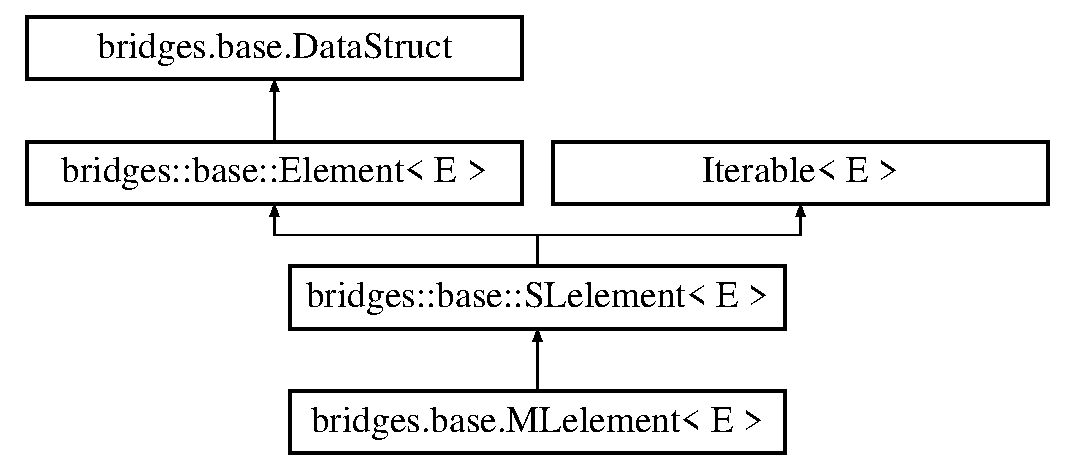
\includegraphics[height=4.000000cm]{classbridges_1_1base_1_1_m_lelement}
\end{center}
\end{figure}


\doxysubsection{Detailed Description}
\begin{DoxyVerb}@brief This class can be used to instantiate Multi-list Elements.
\end{DoxyVerb}


This class extends \mbox{\hyperlink{classbridges_1_1base_1_1_s_lelement}{S\+Lelement}} (singly linked list element) to build multi-\/lists; Multilist elements contain a tag (boolean) that indicates if the element contains a sublist or not; if the tag is true, then there is a sublist beginning at this node and the starting point is the `sublist' field in the element. If the tag is false, then the list continues as a normal singly linked list. The sublists are re recursive\+: any sublist can have its own sublists and so on.

As in singly linked elements, the next pointer points to the following list element and each element contains a generic application specific object. This class extends \mbox{\hyperlink{classbridges_1_1base_1_1_s_lelement}{S\+Lelement}} (singly linked list element) to build multi-\/lists; Multilist elements contain a tag that indicates if the element is a sublist or not; If the element points to a sublist, then the sublist field is the beginning of this sublist. If not, the data field contains the user specified data item and list continues (\mbox{\hyperlink{classbridges_1_1base_1_1_m_lelement_a52ddc26a69eccda5f5b57b94cf87a545}{get\+Next()}}/set\+Next()). As in singly linked elements, the next pointer points to the following list element of the list or sublist. \begin{DoxyVerb}Multi-list elements contain a visualizer (ElementVisualizer) object for setting
\end{DoxyVerb}
 visual attributes (color, shape, opacity, size), necessary for displaying them in a web browser.

Elements also have a \mbox{\hyperlink{classbridges_1_1base_1_1_link_visualizer}{Link\+Visualizer}} object, that is used when they are linked to another element, appropriate for setting link attributes, for instance, between the current element and its next element. In this case, the link in question is that which connects the element to the following elements; a similar logic follows for sublists.

\begin{DoxySeeAlso}{See also}
Example Tutorial at \href{http://bridgesuncc.github.io/tutorials/MultiList.html}{\texttt{ http\+://bridgesuncc.\+github.\+io/tutorials/\+Multi\+List.\+html}}
\end{DoxySeeAlso}
\begin{DoxyAuthor}{Author}
Kalpathi Subramanian
\end{DoxyAuthor}
\begin{DoxyDate}{Date}
5/24/17, 7/14/19
\end{DoxyDate}

\begin{DoxyParams}{Parameters}
{\em E} & The generic parameter object that is part of this element, representing either application specific data, or a pointer to a sublist. \\
\hline
\end{DoxyParams}
\doxysubsection*{Public Member Functions}
\begin{DoxyCompactItemize}
\item 
\mbox{\hyperlink{classbridges_1_1base_1_1_m_lelement_a721d1369c297dc3a3617a1476cb6f5f8}{M\+Lelement}} ()
\item 
\mbox{\hyperlink{classbridges_1_1base_1_1_m_lelement_ad0437d26107039d98cdba6277cff19e2}{M\+Lelement}} (String label, E e)
\item 
\mbox{\hyperlink{classbridges_1_1base_1_1_m_lelement_ad3d5fe59028cd6854eb2abceefad7f7d}{M\+Lelement}} (E e, \mbox{\hyperlink{classbridges_1_1base_1_1_m_lelement}{M\+Lelement}}$<$ E $>$ \mbox{\hyperlink{classbridges_1_1base_1_1_s_lelement_abf61c96a74ad319d561c6952ea388e0e}{next}})
\item 
\mbox{\hyperlink{classbridges_1_1base_1_1_m_lelement_aa660281523a7de140a0b17737096a332}{M\+Lelement}} (\mbox{\hyperlink{classbridges_1_1base_1_1_m_lelement}{M\+Lelement}}$<$ E $>$ sublist, \mbox{\hyperlink{classbridges_1_1base_1_1_m_lelement}{M\+Lelement}}$<$ E $>$ \mbox{\hyperlink{classbridges_1_1base_1_1_s_lelement_abf61c96a74ad319d561c6952ea388e0e}{next}})
\item 
void \mbox{\hyperlink{classbridges_1_1base_1_1_m_lelement_ab13a42b947edc61106ea56c8bd4e78fc}{set\+Sub\+List}} (\mbox{\hyperlink{classbridges_1_1base_1_1_m_lelement}{M\+Lelement}}$<$ E $>$ sl)
\item 
\mbox{\hyperlink{classbridges_1_1base_1_1_m_lelement}{M\+Lelement}} \mbox{\hyperlink{classbridges_1_1base_1_1_m_lelement_afd44cb6e17e16e13a80190747c3b7994}{get\+Sub\+List}} ()
\item 
String \mbox{\hyperlink{classbridges_1_1base_1_1_m_lelement_aa2e26697e2c70a36b8345a324d00679a}{get\+Data\+Struct\+Type}} ()
\item 
\mbox{\hyperlink{classbridges_1_1base_1_1_m_lelement}{M\+Lelement}}$<$ E $>$ \mbox{\hyperlink{classbridges_1_1base_1_1_m_lelement_a52ddc26a69eccda5f5b57b94cf87a545}{get\+Next}} ()
\item 
void \mbox{\hyperlink{classbridges_1_1base_1_1_m_lelement_a60a431ce1b27c98219924075ea764ced}{set\+Tag}} (boolean t)
\item 
boolean \mbox{\hyperlink{classbridges_1_1base_1_1_m_lelement_a95dd0972a3a47cc8ed361cf50508eaa1}{get\+Tag}} ()
\item 
String \mbox{\hyperlink{classbridges_1_1base_1_1_m_lelement_a392f05256ac08e9c19ded1387ebb7583}{get\+Data\+Structure\+Representation}} ()
\end{DoxyCompactItemize}
\doxysubsection*{Protected Member Functions}
\begin{DoxyCompactItemize}
\item 
void \mbox{\hyperlink{classbridges_1_1base_1_1_m_lelement_a496378739f031ef451a6ab1f63c5770f}{get\+List\+Elements}} (Vector$<$ \mbox{\hyperlink{classbridges_1_1base_1_1_element}{Element}}$<$ E $>$$>$ nodes)
\end{DoxyCompactItemize}
\doxysubsection*{Protected Attributes}
\begin{DoxyCompactItemize}
\item 
\mbox{\hyperlink{classbridges_1_1base_1_1_m_lelement}{M\+Lelement}}$<$ E $>$ \mbox{\hyperlink{classbridges_1_1base_1_1_m_lelement_a7dee2985f9a8134d3076eb9478422403}{sub\+\_\+list}} = null
\end{DoxyCompactItemize}


\doxysubsection{Constructor \& Destructor Documentation}
\mbox{\Hypertarget{classbridges_1_1base_1_1_m_lelement_a721d1369c297dc3a3617a1476cb6f5f8}\label{classbridges_1_1base_1_1_m_lelement_a721d1369c297dc3a3617a1476cb6f5f8}} 
\index{bridges.base.MLelement$<$ E $>$@{bridges.base.MLelement$<$ E $>$}!MLelement@{MLelement}}
\index{MLelement@{MLelement}!bridges.base.MLelement$<$ E $>$@{bridges.base.MLelement$<$ E $>$}}
\doxysubsubsection{\texorpdfstring{MLelement()}{MLelement()}\hspace{0.1cm}{\footnotesize\ttfamily [1/4]}}
{\footnotesize\ttfamily \mbox{\hyperlink{classbridges_1_1base_1_1_m_lelement}{bridges.\+base.\+M\+Lelement}}$<$ E $>$.\mbox{\hyperlink{classbridges_1_1base_1_1_m_lelement}{M\+Lelement}} (\begin{DoxyParamCaption}{ }\end{DoxyParamCaption})}

This constructor creates an \mbox{\hyperlink{classbridges_1_1base_1_1_m_lelement}{M\+Lelement}} object and sets the next pointer to null \mbox{\Hypertarget{classbridges_1_1base_1_1_m_lelement_ad0437d26107039d98cdba6277cff19e2}\label{classbridges_1_1base_1_1_m_lelement_ad0437d26107039d98cdba6277cff19e2}} 
\index{bridges.base.MLelement$<$ E $>$@{bridges.base.MLelement$<$ E $>$}!MLelement@{MLelement}}
\index{MLelement@{MLelement}!bridges.base.MLelement$<$ E $>$@{bridges.base.MLelement$<$ E $>$}}
\doxysubsubsection{\texorpdfstring{MLelement()}{MLelement()}\hspace{0.1cm}{\footnotesize\ttfamily [2/4]}}
{\footnotesize\ttfamily \mbox{\hyperlink{classbridges_1_1base_1_1_m_lelement}{bridges.\+base.\+M\+Lelement}}$<$ E $>$.\mbox{\hyperlink{classbridges_1_1base_1_1_m_lelement}{M\+Lelement}} (\begin{DoxyParamCaption}\item[{String}]{label,  }\item[{E}]{e }\end{DoxyParamCaption})}

This constructor creates an \mbox{\hyperlink{classbridges_1_1base_1_1_m_lelement}{M\+Lelement}} object of generic parameter object E, and label \char`\"{}label\char`\"{} and sets the next pointer to null


\begin{DoxyParams}{Parameters}
{\em label} & the label of \mbox{\hyperlink{classbridges_1_1base_1_1_m_lelement}{M\+Lelement}} that shows up on the Bridges visualization \\
\hline
{\em e} & the generic object that this \mbox{\hyperlink{classbridges_1_1base_1_1_m_lelement}{M\+Lelement}} will hold \\
\hline
\end{DoxyParams}
\mbox{\Hypertarget{classbridges_1_1base_1_1_m_lelement_ad3d5fe59028cd6854eb2abceefad7f7d}\label{classbridges_1_1base_1_1_m_lelement_ad3d5fe59028cd6854eb2abceefad7f7d}} 
\index{bridges.base.MLelement$<$ E $>$@{bridges.base.MLelement$<$ E $>$}!MLelement@{MLelement}}
\index{MLelement@{MLelement}!bridges.base.MLelement$<$ E $>$@{bridges.base.MLelement$<$ E $>$}}
\doxysubsubsection{\texorpdfstring{MLelement()}{MLelement()}\hspace{0.1cm}{\footnotesize\ttfamily [3/4]}}
{\footnotesize\ttfamily \mbox{\hyperlink{classbridges_1_1base_1_1_m_lelement}{bridges.\+base.\+M\+Lelement}}$<$ E $>$.\mbox{\hyperlink{classbridges_1_1base_1_1_m_lelement}{M\+Lelement}} (\begin{DoxyParamCaption}\item[{E}]{e,  }\item[{\mbox{\hyperlink{classbridges_1_1base_1_1_m_lelement}{M\+Lelement}}$<$ E $>$}]{next }\end{DoxyParamCaption})}

Creates a new element with value \char`\"{}e\char`\"{} and sets the next pointer to the \mbox{\hyperlink{classbridges_1_1base_1_1_m_lelement}{M\+Lelement}} referenced by the \char`\"{}next\char`\"{} argument


\begin{DoxyParams}{Parameters}
{\em e} & the generic object that this element will hold \\
\hline
{\em next} & the element that should be assigned to the next pointer \\
\hline
\end{DoxyParams}
\mbox{\Hypertarget{classbridges_1_1base_1_1_m_lelement_aa660281523a7de140a0b17737096a332}\label{classbridges_1_1base_1_1_m_lelement_aa660281523a7de140a0b17737096a332}} 
\index{bridges.base.MLelement$<$ E $>$@{bridges.base.MLelement$<$ E $>$}!MLelement@{MLelement}}
\index{MLelement@{MLelement}!bridges.base.MLelement$<$ E $>$@{bridges.base.MLelement$<$ E $>$}}
\doxysubsubsection{\texorpdfstring{MLelement()}{MLelement()}\hspace{0.1cm}{\footnotesize\ttfamily [4/4]}}
{\footnotesize\ttfamily \mbox{\hyperlink{classbridges_1_1base_1_1_m_lelement}{bridges.\+base.\+M\+Lelement}}$<$ E $>$.\mbox{\hyperlink{classbridges_1_1base_1_1_m_lelement}{M\+Lelement}} (\begin{DoxyParamCaption}\item[{\mbox{\hyperlink{classbridges_1_1base_1_1_m_lelement}{M\+Lelement}}$<$ E $>$}]{sublist,  }\item[{\mbox{\hyperlink{classbridges_1_1base_1_1_m_lelement}{M\+Lelement}}$<$ E $>$}]{next }\end{DoxyParamCaption})}

Creates a new element and sets the next pointer to the \mbox{\hyperlink{classbridges_1_1base_1_1_m_lelement}{M\+Lelement}} \char`\"{}next\char`\"{} 
\begin{DoxyParams}{Parameters}
{\em next} & the \mbox{\hyperlink{classbridges_1_1base_1_1_m_lelement}{M\+Lelement}} that should be assigned to the next pointer \\
\hline
\end{DoxyParams}


\doxysubsection{Member Function Documentation}
\mbox{\Hypertarget{classbridges_1_1base_1_1_m_lelement_aa2e26697e2c70a36b8345a324d00679a}\label{classbridges_1_1base_1_1_m_lelement_aa2e26697e2c70a36b8345a324d00679a}} 
\index{bridges.base.MLelement$<$ E $>$@{bridges.base.MLelement$<$ E $>$}!getDataStructType@{getDataStructType}}
\index{getDataStructType@{getDataStructType}!bridges.base.MLelement$<$ E $>$@{bridges.base.MLelement$<$ E $>$}}
\doxysubsubsection{\texorpdfstring{getDataStructType()}{getDataStructType()}}
{\footnotesize\ttfamily String \mbox{\hyperlink{classbridges_1_1base_1_1_m_lelement}{bridges.\+base.\+M\+Lelement}}$<$ E $>$.get\+Data\+Struct\+Type (\begin{DoxyParamCaption}{ }\end{DoxyParamCaption})}

This method gets the data structure type

\begin{DoxyReturn}{Returns}
The date structure type as a string 
\end{DoxyReturn}


Reimplemented from \mbox{\hyperlink{classbridges_1_1base_1_1_s_lelement_a8c48a2d34b238fa0ae7bf2d1ee58ea88}{bridges.\+base.\+S\+Lelement$<$ E $>$}}.

\mbox{\Hypertarget{classbridges_1_1base_1_1_m_lelement_a392f05256ac08e9c19ded1387ebb7583}\label{classbridges_1_1base_1_1_m_lelement_a392f05256ac08e9c19ded1387ebb7583}} 
\index{bridges.base.MLelement$<$ E $>$@{bridges.base.MLelement$<$ E $>$}!getDataStructureRepresentation@{getDataStructureRepresentation}}
\index{getDataStructureRepresentation@{getDataStructureRepresentation}!bridges.base.MLelement$<$ E $>$@{bridges.base.MLelement$<$ E $>$}}
\doxysubsubsection{\texorpdfstring{getDataStructureRepresentation()}{getDataStructureRepresentation()}}
{\footnotesize\ttfamily String \mbox{\hyperlink{classbridges_1_1base_1_1_m_lelement}{bridges.\+base.\+M\+Lelement}}$<$ E $>$.get\+Data\+Structure\+Representation (\begin{DoxyParamCaption}{ }\end{DoxyParamCaption})}

Get the J\+S\+ON representation of the the data structure

\begin{DoxyReturn}{Returns}
the J\+S\+ON string of the element\textquotesingle{}s representation 
\end{DoxyReturn}


Reimplemented from \mbox{\hyperlink{classbridges_1_1base_1_1_s_lelement_a2928f5e8640deaceeecf01adcd75669b}{bridges.\+base.\+S\+Lelement$<$ E $>$}}.

\mbox{\Hypertarget{classbridges_1_1base_1_1_m_lelement_a496378739f031ef451a6ab1f63c5770f}\label{classbridges_1_1base_1_1_m_lelement_a496378739f031ef451a6ab1f63c5770f}} 
\index{bridges.base.MLelement$<$ E $>$@{bridges.base.MLelement$<$ E $>$}!getListElements@{getListElements}}
\index{getListElements@{getListElements}!bridges.base.MLelement$<$ E $>$@{bridges.base.MLelement$<$ E $>$}}
\doxysubsubsection{\texorpdfstring{getListElements()}{getListElements()}}
{\footnotesize\ttfamily void \mbox{\hyperlink{classbridges_1_1base_1_1_m_lelement}{bridges.\+base.\+M\+Lelement}}$<$ E $>$.get\+List\+Elements (\begin{DoxyParamCaption}\item[{Vector$<$ \mbox{\hyperlink{classbridges_1_1base_1_1_element}{Element}}$<$ E $>$$>$}]{nodes }\end{DoxyParamCaption})\hspace{0.3cm}{\ttfamily [protected]}}



Reimplemented from \mbox{\hyperlink{classbridges_1_1base_1_1_s_lelement_abadffea339171349a8e86ded9cd3fe21}{bridges.\+base.\+S\+Lelement$<$ E $>$}}.

\mbox{\Hypertarget{classbridges_1_1base_1_1_m_lelement_a52ddc26a69eccda5f5b57b94cf87a545}\label{classbridges_1_1base_1_1_m_lelement_a52ddc26a69eccda5f5b57b94cf87a545}} 
\index{bridges.base.MLelement$<$ E $>$@{bridges.base.MLelement$<$ E $>$}!getNext@{getNext}}
\index{getNext@{getNext}!bridges.base.MLelement$<$ E $>$@{bridges.base.MLelement$<$ E $>$}}
\doxysubsubsection{\texorpdfstring{getNext()}{getNext()}}
{\footnotesize\ttfamily \mbox{\hyperlink{classbridges_1_1base_1_1_m_lelement}{M\+Lelement}}$<$E$>$ \mbox{\hyperlink{classbridges_1_1base_1_1_m_lelement}{bridges.\+base.\+M\+Lelement}}$<$ E $>$.get\+Next (\begin{DoxyParamCaption}{ }\end{DoxyParamCaption})}

Retrieves the element following this element

\begin{DoxyReturn}{Returns}
M\+Lelement$<$\+E$>$ assigned to next 
\end{DoxyReturn}


Reimplemented from \mbox{\hyperlink{classbridges_1_1base_1_1_s_lelement_a060c4671e05e3f20b16630343393b80d}{bridges.\+base.\+S\+Lelement$<$ E $>$}}.

\mbox{\Hypertarget{classbridges_1_1base_1_1_m_lelement_afd44cb6e17e16e13a80190747c3b7994}\label{classbridges_1_1base_1_1_m_lelement_afd44cb6e17e16e13a80190747c3b7994}} 
\index{bridges.base.MLelement$<$ E $>$@{bridges.base.MLelement$<$ E $>$}!getSubList@{getSubList}}
\index{getSubList@{getSubList}!bridges.base.MLelement$<$ E $>$@{bridges.base.MLelement$<$ E $>$}}
\doxysubsubsection{\texorpdfstring{getSubList()}{getSubList()}}
{\footnotesize\ttfamily \mbox{\hyperlink{classbridges_1_1base_1_1_m_lelement}{M\+Lelement}} \mbox{\hyperlink{classbridges_1_1base_1_1_m_lelement}{bridges.\+base.\+M\+Lelement}}$<$ E $>$.get\+Sub\+List (\begin{DoxyParamCaption}{ }\end{DoxyParamCaption})}

Gets the sublist at this node, if it exists

\begin{DoxyReturn}{Returns}
the sublist head element, if it exists 
\end{DoxyReturn}
\mbox{\Hypertarget{classbridges_1_1base_1_1_m_lelement_a95dd0972a3a47cc8ed361cf50508eaa1}\label{classbridges_1_1base_1_1_m_lelement_a95dd0972a3a47cc8ed361cf50508eaa1}} 
\index{bridges.base.MLelement$<$ E $>$@{bridges.base.MLelement$<$ E $>$}!getTag@{getTag}}
\index{getTag@{getTag}!bridges.base.MLelement$<$ E $>$@{bridges.base.MLelement$<$ E $>$}}
\doxysubsubsection{\texorpdfstring{getTag()}{getTag()}}
{\footnotesize\ttfamily boolean \mbox{\hyperlink{classbridges_1_1base_1_1_m_lelement}{bridges.\+base.\+M\+Lelement}}$<$ E $>$.get\+Tag (\begin{DoxyParamCaption}{ }\end{DoxyParamCaption})}

Gets the tag of the element.

\begin{DoxyReturn}{Returns}
tag of the element 
\end{DoxyReturn}
\mbox{\Hypertarget{classbridges_1_1base_1_1_m_lelement_ab13a42b947edc61106ea56c8bd4e78fc}\label{classbridges_1_1base_1_1_m_lelement_ab13a42b947edc61106ea56c8bd4e78fc}} 
\index{bridges.base.MLelement$<$ E $>$@{bridges.base.MLelement$<$ E $>$}!setSubList@{setSubList}}
\index{setSubList@{setSubList}!bridges.base.MLelement$<$ E $>$@{bridges.base.MLelement$<$ E $>$}}
\doxysubsubsection{\texorpdfstring{setSubList()}{setSubList()}}
{\footnotesize\ttfamily void \mbox{\hyperlink{classbridges_1_1base_1_1_m_lelement}{bridges.\+base.\+M\+Lelement}}$<$ E $>$.set\+Sub\+List (\begin{DoxyParamCaption}\item[{\mbox{\hyperlink{classbridges_1_1base_1_1_m_lelement}{M\+Lelement}}$<$ E $>$}]{sl }\end{DoxyParamCaption})}

Sets the start of a new sublist. to the \mbox{\hyperlink{classbridges_1_1base_1_1_m_lelement}{M\+Lelement}} \char`\"{}next\char`\"{}


\begin{DoxyParams}{Parameters}
{\em sl} & the \mbox{\hyperlink{classbridges_1_1base_1_1_m_lelement}{M\+Lelement}} that is the beginning of a sublist \\
\hline
\end{DoxyParams}
\mbox{\Hypertarget{classbridges_1_1base_1_1_m_lelement_a60a431ce1b27c98219924075ea764ced}\label{classbridges_1_1base_1_1_m_lelement_a60a431ce1b27c98219924075ea764ced}} 
\index{bridges.base.MLelement$<$ E $>$@{bridges.base.MLelement$<$ E $>$}!setTag@{setTag}}
\index{setTag@{setTag}!bridges.base.MLelement$<$ E $>$@{bridges.base.MLelement$<$ E $>$}}
\doxysubsubsection{\texorpdfstring{setTag()}{setTag()}}
{\footnotesize\ttfamily void \mbox{\hyperlink{classbridges_1_1base_1_1_m_lelement}{bridges.\+base.\+M\+Lelement}}$<$ E $>$.set\+Tag (\begin{DoxyParamCaption}\item[{boolean}]{t }\end{DoxyParamCaption})}

Sets the tag of the element.


\begin{DoxyParams}[1]{Parameters}
\mbox{\texttt{ in}}  & {\em t} & tag \\
\hline
\end{DoxyParams}


\doxysubsection{Member Data Documentation}
\mbox{\Hypertarget{classbridges_1_1base_1_1_m_lelement_a7dee2985f9a8134d3076eb9478422403}\label{classbridges_1_1base_1_1_m_lelement_a7dee2985f9a8134d3076eb9478422403}} 
\index{bridges.base.MLelement$<$ E $>$@{bridges.base.MLelement$<$ E $>$}!sub\_list@{sub\_list}}
\index{sub\_list@{sub\_list}!bridges.base.MLelement$<$ E $>$@{bridges.base.MLelement$<$ E $>$}}
\doxysubsubsection{\texorpdfstring{sub\_list}{sub\_list}}
{\footnotesize\ttfamily \mbox{\hyperlink{classbridges_1_1base_1_1_m_lelement}{M\+Lelement}}$<$E$>$ \mbox{\hyperlink{classbridges_1_1base_1_1_m_lelement}{bridges.\+base.\+M\+Lelement}}$<$ E $>$.sub\+\_\+list = null\hspace{0.3cm}{\ttfamily [protected]}}



The documentation for this class was generated from the following file\+:\begin{DoxyCompactItemize}
\item 
/\+Users/kalpathi/gr/bridges/client/java/src/main/java/bridges/base/\mbox{\hyperlink{_m_lelement_8java}{M\+Lelement.\+java}}\end{DoxyCompactItemize}

\hypertarget{enumbridges_1_1base_1_1_named_color}{}\section{bridges.\+base.\+Named\+Color Enum Reference}
\label{enumbridges_1_1base_1_1_named_color}\index{bridges.\+base.\+Named\+Color@{bridges.\+base.\+Named\+Color}}


\subsection{Detailed Description}
This enum is used to represent named, web-\/safe S\+VG colors in B\+R\+I\+D\+G\+ES. 

\begin{DoxyAuthor}{Author}
David Burlinson, 
\end{DoxyAuthor}
\begin{DoxyDate}{Date}
9/06/18 
\end{DoxyDate}
\subsection*{Public Attributes}
\begin{DoxyCompactItemize}
\item 
\hyperlink{enumbridges_1_1base_1_1_named_color_a8d2d3904e6e7f1f6a144365d6fae6b92}{aliceblue}
\item 
\hyperlink{enumbridges_1_1base_1_1_named_color_a49d6e6cad9f1f9c88e2c59eafa78c45c}{antiquewhite}
\item 
\hyperlink{enumbridges_1_1base_1_1_named_color_afe730da1bd9445649a3bb994d3ae6363}{aqua}
\item 
\hyperlink{enumbridges_1_1base_1_1_named_color_a03e600a15631eec7a17cc26ab5a43c04}{aquamarine}
\item 
\hyperlink{enumbridges_1_1base_1_1_named_color_af0ae4fa86b6735a98706ad6c9e898062}{azure}
\item 
\hyperlink{enumbridges_1_1base_1_1_named_color_ad9479f9ff118db34498fe7533a75c416}{beige}
\item 
\hyperlink{enumbridges_1_1base_1_1_named_color_a7cc4c88e0b4f87d4dbfb577cb533c85e}{bisque}
\item 
\hyperlink{enumbridges_1_1base_1_1_named_color_a504b5b12927b738c0f059332e3dc86a4}{black}
\item 
\hyperlink{enumbridges_1_1base_1_1_named_color_a5abdb4bb3f12aa90c0428389f44acaff}{blanchedalmond}
\item 
\hyperlink{enumbridges_1_1base_1_1_named_color_acb31421a17c79934017ff12619686585}{blue}
\item 
\hyperlink{enumbridges_1_1base_1_1_named_color_a4537ee0ae0ccfd3f35acbacbf9dc6ac0}{blueviolet}
\item 
\hyperlink{enumbridges_1_1base_1_1_named_color_a0d2ef5626f9eb4b338eb6b8bb48feaff}{brown}
\item 
\hyperlink{enumbridges_1_1base_1_1_named_color_a8a958193b6e8c98e57771530ac03c07c}{burlywood}
\item 
\hyperlink{enumbridges_1_1base_1_1_named_color_a90675a32f4ac50199c689fd57d971f24}{cadetblue}
\item 
\hyperlink{enumbridges_1_1base_1_1_named_color_a8fd106d773ffb0338f5793421078b117}{chartreuse}
\item 
\hyperlink{enumbridges_1_1base_1_1_named_color_aee60d632523ad71da082647dd8cb5a37}{chocolate}
\item 
\hyperlink{enumbridges_1_1base_1_1_named_color_a3b6a16749bb83786e03b45eaab6f3e12}{coral}
\item 
\hyperlink{enumbridges_1_1base_1_1_named_color_aed29f45dd3fe073058c30968e814bbd4}{cornflowerblue}
\item 
\hyperlink{enumbridges_1_1base_1_1_named_color_a2fac9ce1a766683b727cd23dfe077608}{cornsilk}
\item 
\hyperlink{enumbridges_1_1base_1_1_named_color_ad0ca17e0133f58356bca43aeab1e4b16}{crimson}
\item 
\hyperlink{enumbridges_1_1base_1_1_named_color_ae8c10abf86a217d87a0c0d2569443922}{cyan}
\item 
\hyperlink{enumbridges_1_1base_1_1_named_color_a7ae4391a2d0451d7a079ca7432588aff}{darkblue}
\item 
\hyperlink{enumbridges_1_1base_1_1_named_color_a5060a32b208dedd923cbb7d1cb327839}{darkcyan}
\item 
\hyperlink{enumbridges_1_1base_1_1_named_color_a6b77331712c7f940be58a457aba6f48f}{darkgoldenrod}
\item 
\hyperlink{enumbridges_1_1base_1_1_named_color_a8350298e2fbf7396b25d1de2b852742e}{darkgray}
\item 
\hyperlink{enumbridges_1_1base_1_1_named_color_a3d3f7c76bdd9c3a961af88426f1d8421}{darkgreen}
\item 
\hyperlink{enumbridges_1_1base_1_1_named_color_a183b720b0a9eea34b44388efc3ca5752}{darkgrey}
\item 
\hyperlink{enumbridges_1_1base_1_1_named_color_aeaf7728b7db7eb3a6b558dcbb25c5d6f}{darkkhaki}
\item 
\hyperlink{enumbridges_1_1base_1_1_named_color_a1b3e0db7d2a69d69346403357ceb0c4f}{darkmagenta}
\item 
\hyperlink{enumbridges_1_1base_1_1_named_color_aea7d6d40ed35a490205273a6f1f3391c}{darkolivegreen}
\item 
\hyperlink{enumbridges_1_1base_1_1_named_color_ab7797fb3e19f157f069d329a821aecfa}{darkorange}
\item 
\hyperlink{enumbridges_1_1base_1_1_named_color_a6793d47eb55a097400d40ee2e35be11f}{darkorchid}
\item 
\hyperlink{enumbridges_1_1base_1_1_named_color_a23b8b526a6cf11a154644d982a06acf4}{darkred}
\item 
\hyperlink{enumbridges_1_1base_1_1_named_color_adff8ae5c298919a61b088afae5cae569}{darksalmon}
\item 
\hyperlink{enumbridges_1_1base_1_1_named_color_acd5a590218682162a70aeabaa23befe3}{darkseagreen}
\item 
\hyperlink{enumbridges_1_1base_1_1_named_color_a4c58625c00a2084b128a6373e59b574e}{darkslateblue}
\item 
\hyperlink{enumbridges_1_1base_1_1_named_color_acb1d5dd658644f6deafbcbf033937426}{darkslategray}
\item 
\hyperlink{enumbridges_1_1base_1_1_named_color_a7106cbd702863d8ce275ed11b44ed862}{darkslategrey}
\item 
\hyperlink{enumbridges_1_1base_1_1_named_color_a9b12dc83c3f75bafed12416136e0e262}{darkturquoise}
\item 
\hyperlink{enumbridges_1_1base_1_1_named_color_ab62670e30b318fadc1e5d2998ed5ef03}{darkviolet}
\item 
\hyperlink{enumbridges_1_1base_1_1_named_color_a1fde6d2ba79f40122ad7368256355a83}{deeppink}
\item 
\hyperlink{enumbridges_1_1base_1_1_named_color_a1f5bf5dea5f75f10152fd8d10d61f462}{deepskyblue}
\item 
\hyperlink{enumbridges_1_1base_1_1_named_color_ac9e88827d2e191fad3ce5cbcd096da45}{dimgray}
\item 
\hyperlink{enumbridges_1_1base_1_1_named_color_a6920c8b304105bf147539c1dc68d2541}{dimgrey}
\item 
\hyperlink{enumbridges_1_1base_1_1_named_color_a0be95c59e39316c78ffe13ce5998925d}{dodgerblue}
\item 
\hyperlink{enumbridges_1_1base_1_1_named_color_a7a56091a469c8d113752ee4542fe3b5c}{firebrick}
\item 
\hyperlink{enumbridges_1_1base_1_1_named_color_afe12ca28c9c9f79f19d71822425987ce}{floralwhite}
\item 
\hyperlink{enumbridges_1_1base_1_1_named_color_a324cd709a22d978951a3ba836436be60}{forestgreen}
\item 
\hyperlink{enumbridges_1_1base_1_1_named_color_a16e01cd611d3fcf66a7d1f0bde9d58bb}{fuchsia}
\item 
\hyperlink{enumbridges_1_1base_1_1_named_color_a2ab3edcb33358ebcbbabacf56bd99d8a}{gainsboro}
\item 
\hyperlink{enumbridges_1_1base_1_1_named_color_aac62e3b052d5556715772bbaee2c0fad}{ghostwhite}
\item 
\hyperlink{enumbridges_1_1base_1_1_named_color_a9195a89a01e5bbde2d18a18b733f2e08}{gold}
\item 
\hyperlink{enumbridges_1_1base_1_1_named_color_aa0a94d2e6d4623a213015c4b581fafea}{goldenrod}
\item 
\hyperlink{enumbridges_1_1base_1_1_named_color_ac5a9674778e522abad99f09ca64d269b}{gray}
\item 
\hyperlink{enumbridges_1_1base_1_1_named_color_af2d22a9e15fe27fe2470d7d3af7fe64d}{grey}
\item 
\hyperlink{enumbridges_1_1base_1_1_named_color_a0bf7d23ae5b707f7c02e1144766cca20}{green}
\item 
\hyperlink{enumbridges_1_1base_1_1_named_color_a8c12df0a1f384d1c6dd0920658c4cdda}{greenyellow}
\item 
\hyperlink{enumbridges_1_1base_1_1_named_color_a8ee82cc0f196e1e5b57c0a2f57b2acbd}{honeydew}
\item 
\hyperlink{enumbridges_1_1base_1_1_named_color_ae03fbb40e7b19bae9b7ff76721e5db0a}{hotpink}
\item 
\hyperlink{enumbridges_1_1base_1_1_named_color_a9ff33bb61533fe661006c5716f16fb7c}{indianred}
\item 
\hyperlink{enumbridges_1_1base_1_1_named_color_aa4cea174d807cde767883c3624807555}{indigo}
\item 
\hyperlink{enumbridges_1_1base_1_1_named_color_a9425ce5f3da73a750ea6af05364c050e}{ivory}
\item 
\hyperlink{enumbridges_1_1base_1_1_named_color_a226fd928f639c5b9cfff49556d83c970}{khaki}
\item 
\hyperlink{enumbridges_1_1base_1_1_named_color_af40ede07e5b8876a2bcbb9be4cd54031}{lavender}
\item 
\hyperlink{enumbridges_1_1base_1_1_named_color_a3a6ae081029b076cb1c53fca7cfd187c}{lavenderblush}
\item 
\hyperlink{enumbridges_1_1base_1_1_named_color_a6686557e4f9d73c0b054567f20c7f445}{lawngreen}
\item 
\hyperlink{enumbridges_1_1base_1_1_named_color_a3e7b076971ce4d32b06e637d56eb9f28}{lemonchiffon}
\item 
\hyperlink{enumbridges_1_1base_1_1_named_color_a7e02f0d5b5efdbc1d1b75100e41204fe}{lightblue}
\item 
\hyperlink{enumbridges_1_1base_1_1_named_color_a7788c12b6d0b75601bce3f7d17782e08}{lightcoral}
\item 
\hyperlink{enumbridges_1_1base_1_1_named_color_a18a5f47e2b197763746a42aabe97de58}{lightcyan}
\item 
\hyperlink{enumbridges_1_1base_1_1_named_color_aeefb9dce8b2966401bc3f76c33bb5d47}{lightgoldenrodyellow}
\item 
\hyperlink{enumbridges_1_1base_1_1_named_color_ad7fb6e435204e4e802a7823c80c3aaa9}{lightgray}
\item 
\hyperlink{enumbridges_1_1base_1_1_named_color_a0787c277d0fb832729d89b033a7eb815}{lightgreen}
\item 
\hyperlink{enumbridges_1_1base_1_1_named_color_a34df7602c21ade3a00750cdb0cc264cd}{lightgrey}
\item 
\hyperlink{enumbridges_1_1base_1_1_named_color_a898b5c5b10cef8825c7a943fd07ea97c}{lightpink}
\item 
\hyperlink{enumbridges_1_1base_1_1_named_color_a62c4d992c25987d69947d88108cd0624}{lightsalmon}
\item 
\hyperlink{enumbridges_1_1base_1_1_named_color_a55b9972db6140c1a10be5902d26c3a7f}{lightseagreen}
\item 
\hyperlink{enumbridges_1_1base_1_1_named_color_a7adf26886f0ed7b0d6946a0f1b942f7e}{lightskyblue}
\item 
\hyperlink{enumbridges_1_1base_1_1_named_color_a196667718c28071ef3afd2be06228c71}{lightslategray}
\item 
\hyperlink{enumbridges_1_1base_1_1_named_color_a57070627a1ed7d4c4d14ee8e78dbfea3}{lightslategrey}
\item 
\hyperlink{enumbridges_1_1base_1_1_named_color_afa4c7c3146e112f93df3bd439bd5f66d}{lightsteelblue}
\item 
\hyperlink{enumbridges_1_1base_1_1_named_color_afef38df36fdf63e6abae04c4a2ff3cfc}{lightyellow}
\item 
\hyperlink{enumbridges_1_1base_1_1_named_color_a315145eebf98d49e770f6af2365ef2e0}{lime}
\item 
\hyperlink{enumbridges_1_1base_1_1_named_color_a5692aa381be40fe6564682ab04f97d5e}{limegreen}
\item 
\hyperlink{enumbridges_1_1base_1_1_named_color_afba0725139f792f4e3d3b1f9ba6038e2}{linen}
\item 
\hyperlink{enumbridges_1_1base_1_1_named_color_a222d381e14e181670a111124de9c3a53}{magenta}
\item 
\hyperlink{enumbridges_1_1base_1_1_named_color_a4b47dd1f020e195f32511277f5f930fe}{maroon}
\item 
\hyperlink{enumbridges_1_1base_1_1_named_color_a77c0f823a48e20d395047f3d1b1ec4bb}{mediumaquamarine}
\item 
\hyperlink{enumbridges_1_1base_1_1_named_color_a1039664b375067c2c9cb544c1760b20a}{mediumblue}
\item 
\hyperlink{enumbridges_1_1base_1_1_named_color_acc676c3bf369424334c9ed0d5153cfa4}{mediumorchid}
\item 
\hyperlink{enumbridges_1_1base_1_1_named_color_a16b19da14ae5b34f1f2247dc831a23b7}{mediumpurple}
\item 
\hyperlink{enumbridges_1_1base_1_1_named_color_a34b8a49beabf0428b33a514bd31e40db}{mediumseagreen}
\item 
\hyperlink{enumbridges_1_1base_1_1_named_color_a7560d85c3511ba709a63ad259501b614}{mediumslateblue}
\item 
\hyperlink{enumbridges_1_1base_1_1_named_color_a90acf5312ade0bddfa7408dbfd2f3cec}{mediumspringgreen}
\item 
\hyperlink{enumbridges_1_1base_1_1_named_color_aa7d0d7d1d02271c1ad29acbdfad82e93}{mediumturquoise}
\item 
\hyperlink{enumbridges_1_1base_1_1_named_color_a261f53b5d45d479a4b9657f00fd24e8f}{mediumvioletred}
\item 
\hyperlink{enumbridges_1_1base_1_1_named_color_a33809d07877458903974c5f09e10fa74}{midnightblue}
\item 
\hyperlink{enumbridges_1_1base_1_1_named_color_a59922bad69913e578a9239d3a03e5453}{mintcream}
\item 
\hyperlink{enumbridges_1_1base_1_1_named_color_a5545d40960d882252b92f2d1e8092499}{mistyrose}
\item 
\hyperlink{enumbridges_1_1base_1_1_named_color_ac33aab0e362878493477977d9a97c9fa}{moccasin}
\item 
\hyperlink{enumbridges_1_1base_1_1_named_color_aad5a4d534d028cb567547b3926e303e3}{navajowhite}
\item 
\hyperlink{enumbridges_1_1base_1_1_named_color_a820aac2f4d068ddb43e632e31fbe6421}{navy}
\item 
\hyperlink{enumbridges_1_1base_1_1_named_color_a7ae0332048eb221e34fc099705f2e285}{oldlace}
\item 
\hyperlink{enumbridges_1_1base_1_1_named_color_a86a89ee893b8236c4869fc5602a7dd04}{olive}
\item 
\hyperlink{enumbridges_1_1base_1_1_named_color_aae9f2514ff88caf0f23f991975dc75e2}{olivedrab}
\item 
\hyperlink{enumbridges_1_1base_1_1_named_color_a0cc6a0d16d31d8ceeff99344868c812f}{orange}
\item 
\hyperlink{enumbridges_1_1base_1_1_named_color_abc4e0811a266d71de6e4bd5b7b18d961}{orangered}
\item 
\hyperlink{enumbridges_1_1base_1_1_named_color_a6ba7ed84646316e04fa679c19e6bc08e}{orchid}
\item 
\hyperlink{enumbridges_1_1base_1_1_named_color_a932aad5037d69e4ab2ce2afeb11ff08b}{palegoldenrod}
\item 
\hyperlink{enumbridges_1_1base_1_1_named_color_accbb07c64f164edd041aa56bc6f90b5a}{palegreen}
\item 
\hyperlink{enumbridges_1_1base_1_1_named_color_a9c3c1d8c9cc0c3fb385c6e8ee61e018a}{paleturquoise}
\item 
\hyperlink{enumbridges_1_1base_1_1_named_color_ae4d28e4c1d88fc108b995670d142e2d2}{palevioletred}
\item 
\hyperlink{enumbridges_1_1base_1_1_named_color_adb35f9fa9bdd99fa1f26c8efffbdbdfb}{papayawhip}
\item 
\hyperlink{enumbridges_1_1base_1_1_named_color_a8d436b869b12b7d11ebf473efeec7404}{peachpuff}
\item 
\hyperlink{enumbridges_1_1base_1_1_named_color_a459e1c2697d987a274e028a2d6861631}{peru}
\item 
\hyperlink{enumbridges_1_1base_1_1_named_color_a6aa6a79a9f79af268ea834a18e4f5f58}{pink}
\item 
\hyperlink{enumbridges_1_1base_1_1_named_color_a1660e1c0f9cd3be4534b39b575466217}{plum}
\item 
\hyperlink{enumbridges_1_1base_1_1_named_color_ace97ba9dc403d4af41bf2dc863f01639}{powderblue}
\item 
\hyperlink{enumbridges_1_1base_1_1_named_color_a5f237aa59d1700ea8fc1b7097fa54053}{purple}
\item 
\hyperlink{enumbridges_1_1base_1_1_named_color_a54c42bee9a5b024560317eb2a325452c}{red}
\item 
\hyperlink{enumbridges_1_1base_1_1_named_color_a63e32efb60d734b553b96ecf6437511e}{rosybrown}
\item 
\hyperlink{enumbridges_1_1base_1_1_named_color_a15f4e401c13cbd5171f3819fc9029245}{royalblue}
\item 
\hyperlink{enumbridges_1_1base_1_1_named_color_a8c5ea3615a3581351360eba7cffea3d9}{saddlebrown}
\item 
\hyperlink{enumbridges_1_1base_1_1_named_color_a2dfe2559c4850c23c66c996bdbb6d8f8}{salmon}
\item 
\hyperlink{enumbridges_1_1base_1_1_named_color_a30bcef3dfe65ed4ad51a508bfe90a3d8}{sandybrown}
\item 
\hyperlink{enumbridges_1_1base_1_1_named_color_a4c9395d1d2c270509718a1e1e43d7dff}{seagreen}
\item 
\hyperlink{enumbridges_1_1base_1_1_named_color_a1596f711a2a1e82039b224c37f6ee63a}{seashell}
\item 
\hyperlink{enumbridges_1_1base_1_1_named_color_a28ef2e486839a4a9e67eb4b3b6642b1c}{sienna}
\item 
\hyperlink{enumbridges_1_1base_1_1_named_color_a031901d915bb4950dd0df84fbb63a3a3}{silver}
\item 
\hyperlink{enumbridges_1_1base_1_1_named_color_a1aa829a0ad1f68570f9d94f8994e0a5a}{skyblue}
\item 
\hyperlink{enumbridges_1_1base_1_1_named_color_ae10aa01904e58f56f0ad03c09ab5821b}{slateblue}
\item 
\hyperlink{enumbridges_1_1base_1_1_named_color_a4e79b495b764239831be4f2ace1a727f}{slategray}
\item 
\hyperlink{enumbridges_1_1base_1_1_named_color_a43e40e1c3db71ae925eb8bc37c95a762}{slategrey}
\item 
\hyperlink{enumbridges_1_1base_1_1_named_color_a92ea18875f5defb08e57cc25e61c1df9}{snow}
\item 
\hyperlink{enumbridges_1_1base_1_1_named_color_a7a143a590a72dda8864959e149f5056e}{springgreen}
\item 
\hyperlink{enumbridges_1_1base_1_1_named_color_a7b837b6b35a4cefaccc859c775210971}{steelblue}
\item 
\hyperlink{enumbridges_1_1base_1_1_named_color_ac5ede4192a18ae31ae5ddbbe54f1538b}{tan}
\item 
\hyperlink{enumbridges_1_1base_1_1_named_color_af1b8b9f5b7a4d15a6a610a549f3345a6}{teal}
\item 
\hyperlink{enumbridges_1_1base_1_1_named_color_abc79560d8cf2c7968ad2e9ca0cea6768}{thistle}
\item 
\hyperlink{enumbridges_1_1base_1_1_named_color_a6d6509379946c9dec4e1af978f800994}{tomato}
\item 
\hyperlink{enumbridges_1_1base_1_1_named_color_ac08ba3f77217db505c58bdd323320f62}{turquoise}
\item 
\hyperlink{enumbridges_1_1base_1_1_named_color_aff54fe2bb0b054f29e9f0a9636d299db}{violet}
\item 
\hyperlink{enumbridges_1_1base_1_1_named_color_a93b3cebe6b9ade8be7d4464deeda0247}{wheat}
\item 
\hyperlink{enumbridges_1_1base_1_1_named_color_a1020b159cfe64b5df1c19f1734b5ed34}{white}
\item 
\hyperlink{enumbridges_1_1base_1_1_named_color_aec573e4f20721fb6660fade7a4fcdae7}{whitesmoke}
\item 
\hyperlink{enumbridges_1_1base_1_1_named_color_aaecc9a80f5e566148c7d448424532d95}{yellow}
\item 
\hyperlink{enumbridges_1_1base_1_1_named_color_a263dc51f00db00ef12d4f24cc2c6ee5c}{yellowgreen}
\end{DoxyCompactItemize}


\subsection{Member Data Documentation}
\mbox{\Hypertarget{enumbridges_1_1base_1_1_named_color_a8d2d3904e6e7f1f6a144365d6fae6b92}\label{enumbridges_1_1base_1_1_named_color_a8d2d3904e6e7f1f6a144365d6fae6b92}} 
\index{bridges\+::base\+::\+Named\+Color@{bridges\+::base\+::\+Named\+Color}!aliceblue@{aliceblue}}
\index{aliceblue@{aliceblue}!bridges\+::base\+::\+Named\+Color@{bridges\+::base\+::\+Named\+Color}}
\subsubsection{\texorpdfstring{aliceblue}{aliceblue}}
{\footnotesize\ttfamily bridges.\+base.\+Named\+Color.\+aliceblue}

\mbox{\Hypertarget{enumbridges_1_1base_1_1_named_color_a49d6e6cad9f1f9c88e2c59eafa78c45c}\label{enumbridges_1_1base_1_1_named_color_a49d6e6cad9f1f9c88e2c59eafa78c45c}} 
\index{bridges\+::base\+::\+Named\+Color@{bridges\+::base\+::\+Named\+Color}!antiquewhite@{antiquewhite}}
\index{antiquewhite@{antiquewhite}!bridges\+::base\+::\+Named\+Color@{bridges\+::base\+::\+Named\+Color}}
\subsubsection{\texorpdfstring{antiquewhite}{antiquewhite}}
{\footnotesize\ttfamily bridges.\+base.\+Named\+Color.\+antiquewhite}

\mbox{\Hypertarget{enumbridges_1_1base_1_1_named_color_afe730da1bd9445649a3bb994d3ae6363}\label{enumbridges_1_1base_1_1_named_color_afe730da1bd9445649a3bb994d3ae6363}} 
\index{bridges\+::base\+::\+Named\+Color@{bridges\+::base\+::\+Named\+Color}!aqua@{aqua}}
\index{aqua@{aqua}!bridges\+::base\+::\+Named\+Color@{bridges\+::base\+::\+Named\+Color}}
\subsubsection{\texorpdfstring{aqua}{aqua}}
{\footnotesize\ttfamily bridges.\+base.\+Named\+Color.\+aqua}

\mbox{\Hypertarget{enumbridges_1_1base_1_1_named_color_a03e600a15631eec7a17cc26ab5a43c04}\label{enumbridges_1_1base_1_1_named_color_a03e600a15631eec7a17cc26ab5a43c04}} 
\index{bridges\+::base\+::\+Named\+Color@{bridges\+::base\+::\+Named\+Color}!aquamarine@{aquamarine}}
\index{aquamarine@{aquamarine}!bridges\+::base\+::\+Named\+Color@{bridges\+::base\+::\+Named\+Color}}
\subsubsection{\texorpdfstring{aquamarine}{aquamarine}}
{\footnotesize\ttfamily bridges.\+base.\+Named\+Color.\+aquamarine}

\mbox{\Hypertarget{enumbridges_1_1base_1_1_named_color_af0ae4fa86b6735a98706ad6c9e898062}\label{enumbridges_1_1base_1_1_named_color_af0ae4fa86b6735a98706ad6c9e898062}} 
\index{bridges\+::base\+::\+Named\+Color@{bridges\+::base\+::\+Named\+Color}!azure@{azure}}
\index{azure@{azure}!bridges\+::base\+::\+Named\+Color@{bridges\+::base\+::\+Named\+Color}}
\subsubsection{\texorpdfstring{azure}{azure}}
{\footnotesize\ttfamily bridges.\+base.\+Named\+Color.\+azure}

\mbox{\Hypertarget{enumbridges_1_1base_1_1_named_color_ad9479f9ff118db34498fe7533a75c416}\label{enumbridges_1_1base_1_1_named_color_ad9479f9ff118db34498fe7533a75c416}} 
\index{bridges\+::base\+::\+Named\+Color@{bridges\+::base\+::\+Named\+Color}!beige@{beige}}
\index{beige@{beige}!bridges\+::base\+::\+Named\+Color@{bridges\+::base\+::\+Named\+Color}}
\subsubsection{\texorpdfstring{beige}{beige}}
{\footnotesize\ttfamily bridges.\+base.\+Named\+Color.\+beige}

\mbox{\Hypertarget{enumbridges_1_1base_1_1_named_color_a7cc4c88e0b4f87d4dbfb577cb533c85e}\label{enumbridges_1_1base_1_1_named_color_a7cc4c88e0b4f87d4dbfb577cb533c85e}} 
\index{bridges\+::base\+::\+Named\+Color@{bridges\+::base\+::\+Named\+Color}!bisque@{bisque}}
\index{bisque@{bisque}!bridges\+::base\+::\+Named\+Color@{bridges\+::base\+::\+Named\+Color}}
\subsubsection{\texorpdfstring{bisque}{bisque}}
{\footnotesize\ttfamily bridges.\+base.\+Named\+Color.\+bisque}

\mbox{\Hypertarget{enumbridges_1_1base_1_1_named_color_a504b5b12927b738c0f059332e3dc86a4}\label{enumbridges_1_1base_1_1_named_color_a504b5b12927b738c0f059332e3dc86a4}} 
\index{bridges\+::base\+::\+Named\+Color@{bridges\+::base\+::\+Named\+Color}!black@{black}}
\index{black@{black}!bridges\+::base\+::\+Named\+Color@{bridges\+::base\+::\+Named\+Color}}
\subsubsection{\texorpdfstring{black}{black}}
{\footnotesize\ttfamily bridges.\+base.\+Named\+Color.\+black}

\mbox{\Hypertarget{enumbridges_1_1base_1_1_named_color_a5abdb4bb3f12aa90c0428389f44acaff}\label{enumbridges_1_1base_1_1_named_color_a5abdb4bb3f12aa90c0428389f44acaff}} 
\index{bridges\+::base\+::\+Named\+Color@{bridges\+::base\+::\+Named\+Color}!blanchedalmond@{blanchedalmond}}
\index{blanchedalmond@{blanchedalmond}!bridges\+::base\+::\+Named\+Color@{bridges\+::base\+::\+Named\+Color}}
\subsubsection{\texorpdfstring{blanchedalmond}{blanchedalmond}}
{\footnotesize\ttfamily bridges.\+base.\+Named\+Color.\+blanchedalmond}

\mbox{\Hypertarget{enumbridges_1_1base_1_1_named_color_acb31421a17c79934017ff12619686585}\label{enumbridges_1_1base_1_1_named_color_acb31421a17c79934017ff12619686585}} 
\index{bridges\+::base\+::\+Named\+Color@{bridges\+::base\+::\+Named\+Color}!blue@{blue}}
\index{blue@{blue}!bridges\+::base\+::\+Named\+Color@{bridges\+::base\+::\+Named\+Color}}
\subsubsection{\texorpdfstring{blue}{blue}}
{\footnotesize\ttfamily bridges.\+base.\+Named\+Color.\+blue}

\mbox{\Hypertarget{enumbridges_1_1base_1_1_named_color_a4537ee0ae0ccfd3f35acbacbf9dc6ac0}\label{enumbridges_1_1base_1_1_named_color_a4537ee0ae0ccfd3f35acbacbf9dc6ac0}} 
\index{bridges\+::base\+::\+Named\+Color@{bridges\+::base\+::\+Named\+Color}!blueviolet@{blueviolet}}
\index{blueviolet@{blueviolet}!bridges\+::base\+::\+Named\+Color@{bridges\+::base\+::\+Named\+Color}}
\subsubsection{\texorpdfstring{blueviolet}{blueviolet}}
{\footnotesize\ttfamily bridges.\+base.\+Named\+Color.\+blueviolet}

\mbox{\Hypertarget{enumbridges_1_1base_1_1_named_color_a0d2ef5626f9eb4b338eb6b8bb48feaff}\label{enumbridges_1_1base_1_1_named_color_a0d2ef5626f9eb4b338eb6b8bb48feaff}} 
\index{bridges\+::base\+::\+Named\+Color@{bridges\+::base\+::\+Named\+Color}!brown@{brown}}
\index{brown@{brown}!bridges\+::base\+::\+Named\+Color@{bridges\+::base\+::\+Named\+Color}}
\subsubsection{\texorpdfstring{brown}{brown}}
{\footnotesize\ttfamily bridges.\+base.\+Named\+Color.\+brown}

\mbox{\Hypertarget{enumbridges_1_1base_1_1_named_color_a8a958193b6e8c98e57771530ac03c07c}\label{enumbridges_1_1base_1_1_named_color_a8a958193b6e8c98e57771530ac03c07c}} 
\index{bridges\+::base\+::\+Named\+Color@{bridges\+::base\+::\+Named\+Color}!burlywood@{burlywood}}
\index{burlywood@{burlywood}!bridges\+::base\+::\+Named\+Color@{bridges\+::base\+::\+Named\+Color}}
\subsubsection{\texorpdfstring{burlywood}{burlywood}}
{\footnotesize\ttfamily bridges.\+base.\+Named\+Color.\+burlywood}

\mbox{\Hypertarget{enumbridges_1_1base_1_1_named_color_a90675a32f4ac50199c689fd57d971f24}\label{enumbridges_1_1base_1_1_named_color_a90675a32f4ac50199c689fd57d971f24}} 
\index{bridges\+::base\+::\+Named\+Color@{bridges\+::base\+::\+Named\+Color}!cadetblue@{cadetblue}}
\index{cadetblue@{cadetblue}!bridges\+::base\+::\+Named\+Color@{bridges\+::base\+::\+Named\+Color}}
\subsubsection{\texorpdfstring{cadetblue}{cadetblue}}
{\footnotesize\ttfamily bridges.\+base.\+Named\+Color.\+cadetblue}

\mbox{\Hypertarget{enumbridges_1_1base_1_1_named_color_a8fd106d773ffb0338f5793421078b117}\label{enumbridges_1_1base_1_1_named_color_a8fd106d773ffb0338f5793421078b117}} 
\index{bridges\+::base\+::\+Named\+Color@{bridges\+::base\+::\+Named\+Color}!chartreuse@{chartreuse}}
\index{chartreuse@{chartreuse}!bridges\+::base\+::\+Named\+Color@{bridges\+::base\+::\+Named\+Color}}
\subsubsection{\texorpdfstring{chartreuse}{chartreuse}}
{\footnotesize\ttfamily bridges.\+base.\+Named\+Color.\+chartreuse}

\mbox{\Hypertarget{enumbridges_1_1base_1_1_named_color_aee60d632523ad71da082647dd8cb5a37}\label{enumbridges_1_1base_1_1_named_color_aee60d632523ad71da082647dd8cb5a37}} 
\index{bridges\+::base\+::\+Named\+Color@{bridges\+::base\+::\+Named\+Color}!chocolate@{chocolate}}
\index{chocolate@{chocolate}!bridges\+::base\+::\+Named\+Color@{bridges\+::base\+::\+Named\+Color}}
\subsubsection{\texorpdfstring{chocolate}{chocolate}}
{\footnotesize\ttfamily bridges.\+base.\+Named\+Color.\+chocolate}

\mbox{\Hypertarget{enumbridges_1_1base_1_1_named_color_a3b6a16749bb83786e03b45eaab6f3e12}\label{enumbridges_1_1base_1_1_named_color_a3b6a16749bb83786e03b45eaab6f3e12}} 
\index{bridges\+::base\+::\+Named\+Color@{bridges\+::base\+::\+Named\+Color}!coral@{coral}}
\index{coral@{coral}!bridges\+::base\+::\+Named\+Color@{bridges\+::base\+::\+Named\+Color}}
\subsubsection{\texorpdfstring{coral}{coral}}
{\footnotesize\ttfamily bridges.\+base.\+Named\+Color.\+coral}

\mbox{\Hypertarget{enumbridges_1_1base_1_1_named_color_aed29f45dd3fe073058c30968e814bbd4}\label{enumbridges_1_1base_1_1_named_color_aed29f45dd3fe073058c30968e814bbd4}} 
\index{bridges\+::base\+::\+Named\+Color@{bridges\+::base\+::\+Named\+Color}!cornflowerblue@{cornflowerblue}}
\index{cornflowerblue@{cornflowerblue}!bridges\+::base\+::\+Named\+Color@{bridges\+::base\+::\+Named\+Color}}
\subsubsection{\texorpdfstring{cornflowerblue}{cornflowerblue}}
{\footnotesize\ttfamily bridges.\+base.\+Named\+Color.\+cornflowerblue}

\mbox{\Hypertarget{enumbridges_1_1base_1_1_named_color_a2fac9ce1a766683b727cd23dfe077608}\label{enumbridges_1_1base_1_1_named_color_a2fac9ce1a766683b727cd23dfe077608}} 
\index{bridges\+::base\+::\+Named\+Color@{bridges\+::base\+::\+Named\+Color}!cornsilk@{cornsilk}}
\index{cornsilk@{cornsilk}!bridges\+::base\+::\+Named\+Color@{bridges\+::base\+::\+Named\+Color}}
\subsubsection{\texorpdfstring{cornsilk}{cornsilk}}
{\footnotesize\ttfamily bridges.\+base.\+Named\+Color.\+cornsilk}

\mbox{\Hypertarget{enumbridges_1_1base_1_1_named_color_ad0ca17e0133f58356bca43aeab1e4b16}\label{enumbridges_1_1base_1_1_named_color_ad0ca17e0133f58356bca43aeab1e4b16}} 
\index{bridges\+::base\+::\+Named\+Color@{bridges\+::base\+::\+Named\+Color}!crimson@{crimson}}
\index{crimson@{crimson}!bridges\+::base\+::\+Named\+Color@{bridges\+::base\+::\+Named\+Color}}
\subsubsection{\texorpdfstring{crimson}{crimson}}
{\footnotesize\ttfamily bridges.\+base.\+Named\+Color.\+crimson}

\mbox{\Hypertarget{enumbridges_1_1base_1_1_named_color_ae8c10abf86a217d87a0c0d2569443922}\label{enumbridges_1_1base_1_1_named_color_ae8c10abf86a217d87a0c0d2569443922}} 
\index{bridges\+::base\+::\+Named\+Color@{bridges\+::base\+::\+Named\+Color}!cyan@{cyan}}
\index{cyan@{cyan}!bridges\+::base\+::\+Named\+Color@{bridges\+::base\+::\+Named\+Color}}
\subsubsection{\texorpdfstring{cyan}{cyan}}
{\footnotesize\ttfamily bridges.\+base.\+Named\+Color.\+cyan}

\mbox{\Hypertarget{enumbridges_1_1base_1_1_named_color_a7ae4391a2d0451d7a079ca7432588aff}\label{enumbridges_1_1base_1_1_named_color_a7ae4391a2d0451d7a079ca7432588aff}} 
\index{bridges\+::base\+::\+Named\+Color@{bridges\+::base\+::\+Named\+Color}!darkblue@{darkblue}}
\index{darkblue@{darkblue}!bridges\+::base\+::\+Named\+Color@{bridges\+::base\+::\+Named\+Color}}
\subsubsection{\texorpdfstring{darkblue}{darkblue}}
{\footnotesize\ttfamily bridges.\+base.\+Named\+Color.\+darkblue}

\mbox{\Hypertarget{enumbridges_1_1base_1_1_named_color_a5060a32b208dedd923cbb7d1cb327839}\label{enumbridges_1_1base_1_1_named_color_a5060a32b208dedd923cbb7d1cb327839}} 
\index{bridges\+::base\+::\+Named\+Color@{bridges\+::base\+::\+Named\+Color}!darkcyan@{darkcyan}}
\index{darkcyan@{darkcyan}!bridges\+::base\+::\+Named\+Color@{bridges\+::base\+::\+Named\+Color}}
\subsubsection{\texorpdfstring{darkcyan}{darkcyan}}
{\footnotesize\ttfamily bridges.\+base.\+Named\+Color.\+darkcyan}

\mbox{\Hypertarget{enumbridges_1_1base_1_1_named_color_a6b77331712c7f940be58a457aba6f48f}\label{enumbridges_1_1base_1_1_named_color_a6b77331712c7f940be58a457aba6f48f}} 
\index{bridges\+::base\+::\+Named\+Color@{bridges\+::base\+::\+Named\+Color}!darkgoldenrod@{darkgoldenrod}}
\index{darkgoldenrod@{darkgoldenrod}!bridges\+::base\+::\+Named\+Color@{bridges\+::base\+::\+Named\+Color}}
\subsubsection{\texorpdfstring{darkgoldenrod}{darkgoldenrod}}
{\footnotesize\ttfamily bridges.\+base.\+Named\+Color.\+darkgoldenrod}

\mbox{\Hypertarget{enumbridges_1_1base_1_1_named_color_a8350298e2fbf7396b25d1de2b852742e}\label{enumbridges_1_1base_1_1_named_color_a8350298e2fbf7396b25d1de2b852742e}} 
\index{bridges\+::base\+::\+Named\+Color@{bridges\+::base\+::\+Named\+Color}!darkgray@{darkgray}}
\index{darkgray@{darkgray}!bridges\+::base\+::\+Named\+Color@{bridges\+::base\+::\+Named\+Color}}
\subsubsection{\texorpdfstring{darkgray}{darkgray}}
{\footnotesize\ttfamily bridges.\+base.\+Named\+Color.\+darkgray}

\mbox{\Hypertarget{enumbridges_1_1base_1_1_named_color_a3d3f7c76bdd9c3a961af88426f1d8421}\label{enumbridges_1_1base_1_1_named_color_a3d3f7c76bdd9c3a961af88426f1d8421}} 
\index{bridges\+::base\+::\+Named\+Color@{bridges\+::base\+::\+Named\+Color}!darkgreen@{darkgreen}}
\index{darkgreen@{darkgreen}!bridges\+::base\+::\+Named\+Color@{bridges\+::base\+::\+Named\+Color}}
\subsubsection{\texorpdfstring{darkgreen}{darkgreen}}
{\footnotesize\ttfamily bridges.\+base.\+Named\+Color.\+darkgreen}

\mbox{\Hypertarget{enumbridges_1_1base_1_1_named_color_a183b720b0a9eea34b44388efc3ca5752}\label{enumbridges_1_1base_1_1_named_color_a183b720b0a9eea34b44388efc3ca5752}} 
\index{bridges\+::base\+::\+Named\+Color@{bridges\+::base\+::\+Named\+Color}!darkgrey@{darkgrey}}
\index{darkgrey@{darkgrey}!bridges\+::base\+::\+Named\+Color@{bridges\+::base\+::\+Named\+Color}}
\subsubsection{\texorpdfstring{darkgrey}{darkgrey}}
{\footnotesize\ttfamily bridges.\+base.\+Named\+Color.\+darkgrey}

\mbox{\Hypertarget{enumbridges_1_1base_1_1_named_color_aeaf7728b7db7eb3a6b558dcbb25c5d6f}\label{enumbridges_1_1base_1_1_named_color_aeaf7728b7db7eb3a6b558dcbb25c5d6f}} 
\index{bridges\+::base\+::\+Named\+Color@{bridges\+::base\+::\+Named\+Color}!darkkhaki@{darkkhaki}}
\index{darkkhaki@{darkkhaki}!bridges\+::base\+::\+Named\+Color@{bridges\+::base\+::\+Named\+Color}}
\subsubsection{\texorpdfstring{darkkhaki}{darkkhaki}}
{\footnotesize\ttfamily bridges.\+base.\+Named\+Color.\+darkkhaki}

\mbox{\Hypertarget{enumbridges_1_1base_1_1_named_color_a1b3e0db7d2a69d69346403357ceb0c4f}\label{enumbridges_1_1base_1_1_named_color_a1b3e0db7d2a69d69346403357ceb0c4f}} 
\index{bridges\+::base\+::\+Named\+Color@{bridges\+::base\+::\+Named\+Color}!darkmagenta@{darkmagenta}}
\index{darkmagenta@{darkmagenta}!bridges\+::base\+::\+Named\+Color@{bridges\+::base\+::\+Named\+Color}}
\subsubsection{\texorpdfstring{darkmagenta}{darkmagenta}}
{\footnotesize\ttfamily bridges.\+base.\+Named\+Color.\+darkmagenta}

\mbox{\Hypertarget{enumbridges_1_1base_1_1_named_color_aea7d6d40ed35a490205273a6f1f3391c}\label{enumbridges_1_1base_1_1_named_color_aea7d6d40ed35a490205273a6f1f3391c}} 
\index{bridges\+::base\+::\+Named\+Color@{bridges\+::base\+::\+Named\+Color}!darkolivegreen@{darkolivegreen}}
\index{darkolivegreen@{darkolivegreen}!bridges\+::base\+::\+Named\+Color@{bridges\+::base\+::\+Named\+Color}}
\subsubsection{\texorpdfstring{darkolivegreen}{darkolivegreen}}
{\footnotesize\ttfamily bridges.\+base.\+Named\+Color.\+darkolivegreen}

\mbox{\Hypertarget{enumbridges_1_1base_1_1_named_color_ab7797fb3e19f157f069d329a821aecfa}\label{enumbridges_1_1base_1_1_named_color_ab7797fb3e19f157f069d329a821aecfa}} 
\index{bridges\+::base\+::\+Named\+Color@{bridges\+::base\+::\+Named\+Color}!darkorange@{darkorange}}
\index{darkorange@{darkorange}!bridges\+::base\+::\+Named\+Color@{bridges\+::base\+::\+Named\+Color}}
\subsubsection{\texorpdfstring{darkorange}{darkorange}}
{\footnotesize\ttfamily bridges.\+base.\+Named\+Color.\+darkorange}

\mbox{\Hypertarget{enumbridges_1_1base_1_1_named_color_a6793d47eb55a097400d40ee2e35be11f}\label{enumbridges_1_1base_1_1_named_color_a6793d47eb55a097400d40ee2e35be11f}} 
\index{bridges\+::base\+::\+Named\+Color@{bridges\+::base\+::\+Named\+Color}!darkorchid@{darkorchid}}
\index{darkorchid@{darkorchid}!bridges\+::base\+::\+Named\+Color@{bridges\+::base\+::\+Named\+Color}}
\subsubsection{\texorpdfstring{darkorchid}{darkorchid}}
{\footnotesize\ttfamily bridges.\+base.\+Named\+Color.\+darkorchid}

\mbox{\Hypertarget{enumbridges_1_1base_1_1_named_color_a23b8b526a6cf11a154644d982a06acf4}\label{enumbridges_1_1base_1_1_named_color_a23b8b526a6cf11a154644d982a06acf4}} 
\index{bridges\+::base\+::\+Named\+Color@{bridges\+::base\+::\+Named\+Color}!darkred@{darkred}}
\index{darkred@{darkred}!bridges\+::base\+::\+Named\+Color@{bridges\+::base\+::\+Named\+Color}}
\subsubsection{\texorpdfstring{darkred}{darkred}}
{\footnotesize\ttfamily bridges.\+base.\+Named\+Color.\+darkred}

\mbox{\Hypertarget{enumbridges_1_1base_1_1_named_color_adff8ae5c298919a61b088afae5cae569}\label{enumbridges_1_1base_1_1_named_color_adff8ae5c298919a61b088afae5cae569}} 
\index{bridges\+::base\+::\+Named\+Color@{bridges\+::base\+::\+Named\+Color}!darksalmon@{darksalmon}}
\index{darksalmon@{darksalmon}!bridges\+::base\+::\+Named\+Color@{bridges\+::base\+::\+Named\+Color}}
\subsubsection{\texorpdfstring{darksalmon}{darksalmon}}
{\footnotesize\ttfamily bridges.\+base.\+Named\+Color.\+darksalmon}

\mbox{\Hypertarget{enumbridges_1_1base_1_1_named_color_acd5a590218682162a70aeabaa23befe3}\label{enumbridges_1_1base_1_1_named_color_acd5a590218682162a70aeabaa23befe3}} 
\index{bridges\+::base\+::\+Named\+Color@{bridges\+::base\+::\+Named\+Color}!darkseagreen@{darkseagreen}}
\index{darkseagreen@{darkseagreen}!bridges\+::base\+::\+Named\+Color@{bridges\+::base\+::\+Named\+Color}}
\subsubsection{\texorpdfstring{darkseagreen}{darkseagreen}}
{\footnotesize\ttfamily bridges.\+base.\+Named\+Color.\+darkseagreen}

\mbox{\Hypertarget{enumbridges_1_1base_1_1_named_color_a4c58625c00a2084b128a6373e59b574e}\label{enumbridges_1_1base_1_1_named_color_a4c58625c00a2084b128a6373e59b574e}} 
\index{bridges\+::base\+::\+Named\+Color@{bridges\+::base\+::\+Named\+Color}!darkslateblue@{darkslateblue}}
\index{darkslateblue@{darkslateblue}!bridges\+::base\+::\+Named\+Color@{bridges\+::base\+::\+Named\+Color}}
\subsubsection{\texorpdfstring{darkslateblue}{darkslateblue}}
{\footnotesize\ttfamily bridges.\+base.\+Named\+Color.\+darkslateblue}

\mbox{\Hypertarget{enumbridges_1_1base_1_1_named_color_acb1d5dd658644f6deafbcbf033937426}\label{enumbridges_1_1base_1_1_named_color_acb1d5dd658644f6deafbcbf033937426}} 
\index{bridges\+::base\+::\+Named\+Color@{bridges\+::base\+::\+Named\+Color}!darkslategray@{darkslategray}}
\index{darkslategray@{darkslategray}!bridges\+::base\+::\+Named\+Color@{bridges\+::base\+::\+Named\+Color}}
\subsubsection{\texorpdfstring{darkslategray}{darkslategray}}
{\footnotesize\ttfamily bridges.\+base.\+Named\+Color.\+darkslategray}

\mbox{\Hypertarget{enumbridges_1_1base_1_1_named_color_a7106cbd702863d8ce275ed11b44ed862}\label{enumbridges_1_1base_1_1_named_color_a7106cbd702863d8ce275ed11b44ed862}} 
\index{bridges\+::base\+::\+Named\+Color@{bridges\+::base\+::\+Named\+Color}!darkslategrey@{darkslategrey}}
\index{darkslategrey@{darkslategrey}!bridges\+::base\+::\+Named\+Color@{bridges\+::base\+::\+Named\+Color}}
\subsubsection{\texorpdfstring{darkslategrey}{darkslategrey}}
{\footnotesize\ttfamily bridges.\+base.\+Named\+Color.\+darkslategrey}

\mbox{\Hypertarget{enumbridges_1_1base_1_1_named_color_a9b12dc83c3f75bafed12416136e0e262}\label{enumbridges_1_1base_1_1_named_color_a9b12dc83c3f75bafed12416136e0e262}} 
\index{bridges\+::base\+::\+Named\+Color@{bridges\+::base\+::\+Named\+Color}!darkturquoise@{darkturquoise}}
\index{darkturquoise@{darkturquoise}!bridges\+::base\+::\+Named\+Color@{bridges\+::base\+::\+Named\+Color}}
\subsubsection{\texorpdfstring{darkturquoise}{darkturquoise}}
{\footnotesize\ttfamily bridges.\+base.\+Named\+Color.\+darkturquoise}

\mbox{\Hypertarget{enumbridges_1_1base_1_1_named_color_ab62670e30b318fadc1e5d2998ed5ef03}\label{enumbridges_1_1base_1_1_named_color_ab62670e30b318fadc1e5d2998ed5ef03}} 
\index{bridges\+::base\+::\+Named\+Color@{bridges\+::base\+::\+Named\+Color}!darkviolet@{darkviolet}}
\index{darkviolet@{darkviolet}!bridges\+::base\+::\+Named\+Color@{bridges\+::base\+::\+Named\+Color}}
\subsubsection{\texorpdfstring{darkviolet}{darkviolet}}
{\footnotesize\ttfamily bridges.\+base.\+Named\+Color.\+darkviolet}

\mbox{\Hypertarget{enumbridges_1_1base_1_1_named_color_a1fde6d2ba79f40122ad7368256355a83}\label{enumbridges_1_1base_1_1_named_color_a1fde6d2ba79f40122ad7368256355a83}} 
\index{bridges\+::base\+::\+Named\+Color@{bridges\+::base\+::\+Named\+Color}!deeppink@{deeppink}}
\index{deeppink@{deeppink}!bridges\+::base\+::\+Named\+Color@{bridges\+::base\+::\+Named\+Color}}
\subsubsection{\texorpdfstring{deeppink}{deeppink}}
{\footnotesize\ttfamily bridges.\+base.\+Named\+Color.\+deeppink}

\mbox{\Hypertarget{enumbridges_1_1base_1_1_named_color_a1f5bf5dea5f75f10152fd8d10d61f462}\label{enumbridges_1_1base_1_1_named_color_a1f5bf5dea5f75f10152fd8d10d61f462}} 
\index{bridges\+::base\+::\+Named\+Color@{bridges\+::base\+::\+Named\+Color}!deepskyblue@{deepskyblue}}
\index{deepskyblue@{deepskyblue}!bridges\+::base\+::\+Named\+Color@{bridges\+::base\+::\+Named\+Color}}
\subsubsection{\texorpdfstring{deepskyblue}{deepskyblue}}
{\footnotesize\ttfamily bridges.\+base.\+Named\+Color.\+deepskyblue}

\mbox{\Hypertarget{enumbridges_1_1base_1_1_named_color_ac9e88827d2e191fad3ce5cbcd096da45}\label{enumbridges_1_1base_1_1_named_color_ac9e88827d2e191fad3ce5cbcd096da45}} 
\index{bridges\+::base\+::\+Named\+Color@{bridges\+::base\+::\+Named\+Color}!dimgray@{dimgray}}
\index{dimgray@{dimgray}!bridges\+::base\+::\+Named\+Color@{bridges\+::base\+::\+Named\+Color}}
\subsubsection{\texorpdfstring{dimgray}{dimgray}}
{\footnotesize\ttfamily bridges.\+base.\+Named\+Color.\+dimgray}

\mbox{\Hypertarget{enumbridges_1_1base_1_1_named_color_a6920c8b304105bf147539c1dc68d2541}\label{enumbridges_1_1base_1_1_named_color_a6920c8b304105bf147539c1dc68d2541}} 
\index{bridges\+::base\+::\+Named\+Color@{bridges\+::base\+::\+Named\+Color}!dimgrey@{dimgrey}}
\index{dimgrey@{dimgrey}!bridges\+::base\+::\+Named\+Color@{bridges\+::base\+::\+Named\+Color}}
\subsubsection{\texorpdfstring{dimgrey}{dimgrey}}
{\footnotesize\ttfamily bridges.\+base.\+Named\+Color.\+dimgrey}

\mbox{\Hypertarget{enumbridges_1_1base_1_1_named_color_a0be95c59e39316c78ffe13ce5998925d}\label{enumbridges_1_1base_1_1_named_color_a0be95c59e39316c78ffe13ce5998925d}} 
\index{bridges\+::base\+::\+Named\+Color@{bridges\+::base\+::\+Named\+Color}!dodgerblue@{dodgerblue}}
\index{dodgerblue@{dodgerblue}!bridges\+::base\+::\+Named\+Color@{bridges\+::base\+::\+Named\+Color}}
\subsubsection{\texorpdfstring{dodgerblue}{dodgerblue}}
{\footnotesize\ttfamily bridges.\+base.\+Named\+Color.\+dodgerblue}

\mbox{\Hypertarget{enumbridges_1_1base_1_1_named_color_a7a56091a469c8d113752ee4542fe3b5c}\label{enumbridges_1_1base_1_1_named_color_a7a56091a469c8d113752ee4542fe3b5c}} 
\index{bridges\+::base\+::\+Named\+Color@{bridges\+::base\+::\+Named\+Color}!firebrick@{firebrick}}
\index{firebrick@{firebrick}!bridges\+::base\+::\+Named\+Color@{bridges\+::base\+::\+Named\+Color}}
\subsubsection{\texorpdfstring{firebrick}{firebrick}}
{\footnotesize\ttfamily bridges.\+base.\+Named\+Color.\+firebrick}

\mbox{\Hypertarget{enumbridges_1_1base_1_1_named_color_afe12ca28c9c9f79f19d71822425987ce}\label{enumbridges_1_1base_1_1_named_color_afe12ca28c9c9f79f19d71822425987ce}} 
\index{bridges\+::base\+::\+Named\+Color@{bridges\+::base\+::\+Named\+Color}!floralwhite@{floralwhite}}
\index{floralwhite@{floralwhite}!bridges\+::base\+::\+Named\+Color@{bridges\+::base\+::\+Named\+Color}}
\subsubsection{\texorpdfstring{floralwhite}{floralwhite}}
{\footnotesize\ttfamily bridges.\+base.\+Named\+Color.\+floralwhite}

\mbox{\Hypertarget{enumbridges_1_1base_1_1_named_color_a324cd709a22d978951a3ba836436be60}\label{enumbridges_1_1base_1_1_named_color_a324cd709a22d978951a3ba836436be60}} 
\index{bridges\+::base\+::\+Named\+Color@{bridges\+::base\+::\+Named\+Color}!forestgreen@{forestgreen}}
\index{forestgreen@{forestgreen}!bridges\+::base\+::\+Named\+Color@{bridges\+::base\+::\+Named\+Color}}
\subsubsection{\texorpdfstring{forestgreen}{forestgreen}}
{\footnotesize\ttfamily bridges.\+base.\+Named\+Color.\+forestgreen}

\mbox{\Hypertarget{enumbridges_1_1base_1_1_named_color_a16e01cd611d3fcf66a7d1f0bde9d58bb}\label{enumbridges_1_1base_1_1_named_color_a16e01cd611d3fcf66a7d1f0bde9d58bb}} 
\index{bridges\+::base\+::\+Named\+Color@{bridges\+::base\+::\+Named\+Color}!fuchsia@{fuchsia}}
\index{fuchsia@{fuchsia}!bridges\+::base\+::\+Named\+Color@{bridges\+::base\+::\+Named\+Color}}
\subsubsection{\texorpdfstring{fuchsia}{fuchsia}}
{\footnotesize\ttfamily bridges.\+base.\+Named\+Color.\+fuchsia}

\mbox{\Hypertarget{enumbridges_1_1base_1_1_named_color_a2ab3edcb33358ebcbbabacf56bd99d8a}\label{enumbridges_1_1base_1_1_named_color_a2ab3edcb33358ebcbbabacf56bd99d8a}} 
\index{bridges\+::base\+::\+Named\+Color@{bridges\+::base\+::\+Named\+Color}!gainsboro@{gainsboro}}
\index{gainsboro@{gainsboro}!bridges\+::base\+::\+Named\+Color@{bridges\+::base\+::\+Named\+Color}}
\subsubsection{\texorpdfstring{gainsboro}{gainsboro}}
{\footnotesize\ttfamily bridges.\+base.\+Named\+Color.\+gainsboro}

\mbox{\Hypertarget{enumbridges_1_1base_1_1_named_color_aac62e3b052d5556715772bbaee2c0fad}\label{enumbridges_1_1base_1_1_named_color_aac62e3b052d5556715772bbaee2c0fad}} 
\index{bridges\+::base\+::\+Named\+Color@{bridges\+::base\+::\+Named\+Color}!ghostwhite@{ghostwhite}}
\index{ghostwhite@{ghostwhite}!bridges\+::base\+::\+Named\+Color@{bridges\+::base\+::\+Named\+Color}}
\subsubsection{\texorpdfstring{ghostwhite}{ghostwhite}}
{\footnotesize\ttfamily bridges.\+base.\+Named\+Color.\+ghostwhite}

\mbox{\Hypertarget{enumbridges_1_1base_1_1_named_color_a9195a89a01e5bbde2d18a18b733f2e08}\label{enumbridges_1_1base_1_1_named_color_a9195a89a01e5bbde2d18a18b733f2e08}} 
\index{bridges\+::base\+::\+Named\+Color@{bridges\+::base\+::\+Named\+Color}!gold@{gold}}
\index{gold@{gold}!bridges\+::base\+::\+Named\+Color@{bridges\+::base\+::\+Named\+Color}}
\subsubsection{\texorpdfstring{gold}{gold}}
{\footnotesize\ttfamily bridges.\+base.\+Named\+Color.\+gold}

\mbox{\Hypertarget{enumbridges_1_1base_1_1_named_color_aa0a94d2e6d4623a213015c4b581fafea}\label{enumbridges_1_1base_1_1_named_color_aa0a94d2e6d4623a213015c4b581fafea}} 
\index{bridges\+::base\+::\+Named\+Color@{bridges\+::base\+::\+Named\+Color}!goldenrod@{goldenrod}}
\index{goldenrod@{goldenrod}!bridges\+::base\+::\+Named\+Color@{bridges\+::base\+::\+Named\+Color}}
\subsubsection{\texorpdfstring{goldenrod}{goldenrod}}
{\footnotesize\ttfamily bridges.\+base.\+Named\+Color.\+goldenrod}

\mbox{\Hypertarget{enumbridges_1_1base_1_1_named_color_ac5a9674778e522abad99f09ca64d269b}\label{enumbridges_1_1base_1_1_named_color_ac5a9674778e522abad99f09ca64d269b}} 
\index{bridges\+::base\+::\+Named\+Color@{bridges\+::base\+::\+Named\+Color}!gray@{gray}}
\index{gray@{gray}!bridges\+::base\+::\+Named\+Color@{bridges\+::base\+::\+Named\+Color}}
\subsubsection{\texorpdfstring{gray}{gray}}
{\footnotesize\ttfamily bridges.\+base.\+Named\+Color.\+gray}

\mbox{\Hypertarget{enumbridges_1_1base_1_1_named_color_a0bf7d23ae5b707f7c02e1144766cca20}\label{enumbridges_1_1base_1_1_named_color_a0bf7d23ae5b707f7c02e1144766cca20}} 
\index{bridges\+::base\+::\+Named\+Color@{bridges\+::base\+::\+Named\+Color}!green@{green}}
\index{green@{green}!bridges\+::base\+::\+Named\+Color@{bridges\+::base\+::\+Named\+Color}}
\subsubsection{\texorpdfstring{green}{green}}
{\footnotesize\ttfamily bridges.\+base.\+Named\+Color.\+green}

\mbox{\Hypertarget{enumbridges_1_1base_1_1_named_color_a8c12df0a1f384d1c6dd0920658c4cdda}\label{enumbridges_1_1base_1_1_named_color_a8c12df0a1f384d1c6dd0920658c4cdda}} 
\index{bridges\+::base\+::\+Named\+Color@{bridges\+::base\+::\+Named\+Color}!greenyellow@{greenyellow}}
\index{greenyellow@{greenyellow}!bridges\+::base\+::\+Named\+Color@{bridges\+::base\+::\+Named\+Color}}
\subsubsection{\texorpdfstring{greenyellow}{greenyellow}}
{\footnotesize\ttfamily bridges.\+base.\+Named\+Color.\+greenyellow}

\mbox{\Hypertarget{enumbridges_1_1base_1_1_named_color_af2d22a9e15fe27fe2470d7d3af7fe64d}\label{enumbridges_1_1base_1_1_named_color_af2d22a9e15fe27fe2470d7d3af7fe64d}} 
\index{bridges\+::base\+::\+Named\+Color@{bridges\+::base\+::\+Named\+Color}!grey@{grey}}
\index{grey@{grey}!bridges\+::base\+::\+Named\+Color@{bridges\+::base\+::\+Named\+Color}}
\subsubsection{\texorpdfstring{grey}{grey}}
{\footnotesize\ttfamily bridges.\+base.\+Named\+Color.\+grey}

\mbox{\Hypertarget{enumbridges_1_1base_1_1_named_color_a8ee82cc0f196e1e5b57c0a2f57b2acbd}\label{enumbridges_1_1base_1_1_named_color_a8ee82cc0f196e1e5b57c0a2f57b2acbd}} 
\index{bridges\+::base\+::\+Named\+Color@{bridges\+::base\+::\+Named\+Color}!honeydew@{honeydew}}
\index{honeydew@{honeydew}!bridges\+::base\+::\+Named\+Color@{bridges\+::base\+::\+Named\+Color}}
\subsubsection{\texorpdfstring{honeydew}{honeydew}}
{\footnotesize\ttfamily bridges.\+base.\+Named\+Color.\+honeydew}

\mbox{\Hypertarget{enumbridges_1_1base_1_1_named_color_ae03fbb40e7b19bae9b7ff76721e5db0a}\label{enumbridges_1_1base_1_1_named_color_ae03fbb40e7b19bae9b7ff76721e5db0a}} 
\index{bridges\+::base\+::\+Named\+Color@{bridges\+::base\+::\+Named\+Color}!hotpink@{hotpink}}
\index{hotpink@{hotpink}!bridges\+::base\+::\+Named\+Color@{bridges\+::base\+::\+Named\+Color}}
\subsubsection{\texorpdfstring{hotpink}{hotpink}}
{\footnotesize\ttfamily bridges.\+base.\+Named\+Color.\+hotpink}

\mbox{\Hypertarget{enumbridges_1_1base_1_1_named_color_a9ff33bb61533fe661006c5716f16fb7c}\label{enumbridges_1_1base_1_1_named_color_a9ff33bb61533fe661006c5716f16fb7c}} 
\index{bridges\+::base\+::\+Named\+Color@{bridges\+::base\+::\+Named\+Color}!indianred@{indianred}}
\index{indianred@{indianred}!bridges\+::base\+::\+Named\+Color@{bridges\+::base\+::\+Named\+Color}}
\subsubsection{\texorpdfstring{indianred}{indianred}}
{\footnotesize\ttfamily bridges.\+base.\+Named\+Color.\+indianred}

\mbox{\Hypertarget{enumbridges_1_1base_1_1_named_color_aa4cea174d807cde767883c3624807555}\label{enumbridges_1_1base_1_1_named_color_aa4cea174d807cde767883c3624807555}} 
\index{bridges\+::base\+::\+Named\+Color@{bridges\+::base\+::\+Named\+Color}!indigo@{indigo}}
\index{indigo@{indigo}!bridges\+::base\+::\+Named\+Color@{bridges\+::base\+::\+Named\+Color}}
\subsubsection{\texorpdfstring{indigo}{indigo}}
{\footnotesize\ttfamily bridges.\+base.\+Named\+Color.\+indigo}

\mbox{\Hypertarget{enumbridges_1_1base_1_1_named_color_a9425ce5f3da73a750ea6af05364c050e}\label{enumbridges_1_1base_1_1_named_color_a9425ce5f3da73a750ea6af05364c050e}} 
\index{bridges\+::base\+::\+Named\+Color@{bridges\+::base\+::\+Named\+Color}!ivory@{ivory}}
\index{ivory@{ivory}!bridges\+::base\+::\+Named\+Color@{bridges\+::base\+::\+Named\+Color}}
\subsubsection{\texorpdfstring{ivory}{ivory}}
{\footnotesize\ttfamily bridges.\+base.\+Named\+Color.\+ivory}

\mbox{\Hypertarget{enumbridges_1_1base_1_1_named_color_a226fd928f639c5b9cfff49556d83c970}\label{enumbridges_1_1base_1_1_named_color_a226fd928f639c5b9cfff49556d83c970}} 
\index{bridges\+::base\+::\+Named\+Color@{bridges\+::base\+::\+Named\+Color}!khaki@{khaki}}
\index{khaki@{khaki}!bridges\+::base\+::\+Named\+Color@{bridges\+::base\+::\+Named\+Color}}
\subsubsection{\texorpdfstring{khaki}{khaki}}
{\footnotesize\ttfamily bridges.\+base.\+Named\+Color.\+khaki}

\mbox{\Hypertarget{enumbridges_1_1base_1_1_named_color_af40ede07e5b8876a2bcbb9be4cd54031}\label{enumbridges_1_1base_1_1_named_color_af40ede07e5b8876a2bcbb9be4cd54031}} 
\index{bridges\+::base\+::\+Named\+Color@{bridges\+::base\+::\+Named\+Color}!lavender@{lavender}}
\index{lavender@{lavender}!bridges\+::base\+::\+Named\+Color@{bridges\+::base\+::\+Named\+Color}}
\subsubsection{\texorpdfstring{lavender}{lavender}}
{\footnotesize\ttfamily bridges.\+base.\+Named\+Color.\+lavender}

\mbox{\Hypertarget{enumbridges_1_1base_1_1_named_color_a3a6ae081029b076cb1c53fca7cfd187c}\label{enumbridges_1_1base_1_1_named_color_a3a6ae081029b076cb1c53fca7cfd187c}} 
\index{bridges\+::base\+::\+Named\+Color@{bridges\+::base\+::\+Named\+Color}!lavenderblush@{lavenderblush}}
\index{lavenderblush@{lavenderblush}!bridges\+::base\+::\+Named\+Color@{bridges\+::base\+::\+Named\+Color}}
\subsubsection{\texorpdfstring{lavenderblush}{lavenderblush}}
{\footnotesize\ttfamily bridges.\+base.\+Named\+Color.\+lavenderblush}

\mbox{\Hypertarget{enumbridges_1_1base_1_1_named_color_a6686557e4f9d73c0b054567f20c7f445}\label{enumbridges_1_1base_1_1_named_color_a6686557e4f9d73c0b054567f20c7f445}} 
\index{bridges\+::base\+::\+Named\+Color@{bridges\+::base\+::\+Named\+Color}!lawngreen@{lawngreen}}
\index{lawngreen@{lawngreen}!bridges\+::base\+::\+Named\+Color@{bridges\+::base\+::\+Named\+Color}}
\subsubsection{\texorpdfstring{lawngreen}{lawngreen}}
{\footnotesize\ttfamily bridges.\+base.\+Named\+Color.\+lawngreen}

\mbox{\Hypertarget{enumbridges_1_1base_1_1_named_color_a3e7b076971ce4d32b06e637d56eb9f28}\label{enumbridges_1_1base_1_1_named_color_a3e7b076971ce4d32b06e637d56eb9f28}} 
\index{bridges\+::base\+::\+Named\+Color@{bridges\+::base\+::\+Named\+Color}!lemonchiffon@{lemonchiffon}}
\index{lemonchiffon@{lemonchiffon}!bridges\+::base\+::\+Named\+Color@{bridges\+::base\+::\+Named\+Color}}
\subsubsection{\texorpdfstring{lemonchiffon}{lemonchiffon}}
{\footnotesize\ttfamily bridges.\+base.\+Named\+Color.\+lemonchiffon}

\mbox{\Hypertarget{enumbridges_1_1base_1_1_named_color_a7e02f0d5b5efdbc1d1b75100e41204fe}\label{enumbridges_1_1base_1_1_named_color_a7e02f0d5b5efdbc1d1b75100e41204fe}} 
\index{bridges\+::base\+::\+Named\+Color@{bridges\+::base\+::\+Named\+Color}!lightblue@{lightblue}}
\index{lightblue@{lightblue}!bridges\+::base\+::\+Named\+Color@{bridges\+::base\+::\+Named\+Color}}
\subsubsection{\texorpdfstring{lightblue}{lightblue}}
{\footnotesize\ttfamily bridges.\+base.\+Named\+Color.\+lightblue}

\mbox{\Hypertarget{enumbridges_1_1base_1_1_named_color_a7788c12b6d0b75601bce3f7d17782e08}\label{enumbridges_1_1base_1_1_named_color_a7788c12b6d0b75601bce3f7d17782e08}} 
\index{bridges\+::base\+::\+Named\+Color@{bridges\+::base\+::\+Named\+Color}!lightcoral@{lightcoral}}
\index{lightcoral@{lightcoral}!bridges\+::base\+::\+Named\+Color@{bridges\+::base\+::\+Named\+Color}}
\subsubsection{\texorpdfstring{lightcoral}{lightcoral}}
{\footnotesize\ttfamily bridges.\+base.\+Named\+Color.\+lightcoral}

\mbox{\Hypertarget{enumbridges_1_1base_1_1_named_color_a18a5f47e2b197763746a42aabe97de58}\label{enumbridges_1_1base_1_1_named_color_a18a5f47e2b197763746a42aabe97de58}} 
\index{bridges\+::base\+::\+Named\+Color@{bridges\+::base\+::\+Named\+Color}!lightcyan@{lightcyan}}
\index{lightcyan@{lightcyan}!bridges\+::base\+::\+Named\+Color@{bridges\+::base\+::\+Named\+Color}}
\subsubsection{\texorpdfstring{lightcyan}{lightcyan}}
{\footnotesize\ttfamily bridges.\+base.\+Named\+Color.\+lightcyan}

\mbox{\Hypertarget{enumbridges_1_1base_1_1_named_color_aeefb9dce8b2966401bc3f76c33bb5d47}\label{enumbridges_1_1base_1_1_named_color_aeefb9dce8b2966401bc3f76c33bb5d47}} 
\index{bridges\+::base\+::\+Named\+Color@{bridges\+::base\+::\+Named\+Color}!lightgoldenrodyellow@{lightgoldenrodyellow}}
\index{lightgoldenrodyellow@{lightgoldenrodyellow}!bridges\+::base\+::\+Named\+Color@{bridges\+::base\+::\+Named\+Color}}
\subsubsection{\texorpdfstring{lightgoldenrodyellow}{lightgoldenrodyellow}}
{\footnotesize\ttfamily bridges.\+base.\+Named\+Color.\+lightgoldenrodyellow}

\mbox{\Hypertarget{enumbridges_1_1base_1_1_named_color_ad7fb6e435204e4e802a7823c80c3aaa9}\label{enumbridges_1_1base_1_1_named_color_ad7fb6e435204e4e802a7823c80c3aaa9}} 
\index{bridges\+::base\+::\+Named\+Color@{bridges\+::base\+::\+Named\+Color}!lightgray@{lightgray}}
\index{lightgray@{lightgray}!bridges\+::base\+::\+Named\+Color@{bridges\+::base\+::\+Named\+Color}}
\subsubsection{\texorpdfstring{lightgray}{lightgray}}
{\footnotesize\ttfamily bridges.\+base.\+Named\+Color.\+lightgray}

\mbox{\Hypertarget{enumbridges_1_1base_1_1_named_color_a0787c277d0fb832729d89b033a7eb815}\label{enumbridges_1_1base_1_1_named_color_a0787c277d0fb832729d89b033a7eb815}} 
\index{bridges\+::base\+::\+Named\+Color@{bridges\+::base\+::\+Named\+Color}!lightgreen@{lightgreen}}
\index{lightgreen@{lightgreen}!bridges\+::base\+::\+Named\+Color@{bridges\+::base\+::\+Named\+Color}}
\subsubsection{\texorpdfstring{lightgreen}{lightgreen}}
{\footnotesize\ttfamily bridges.\+base.\+Named\+Color.\+lightgreen}

\mbox{\Hypertarget{enumbridges_1_1base_1_1_named_color_a34df7602c21ade3a00750cdb0cc264cd}\label{enumbridges_1_1base_1_1_named_color_a34df7602c21ade3a00750cdb0cc264cd}} 
\index{bridges\+::base\+::\+Named\+Color@{bridges\+::base\+::\+Named\+Color}!lightgrey@{lightgrey}}
\index{lightgrey@{lightgrey}!bridges\+::base\+::\+Named\+Color@{bridges\+::base\+::\+Named\+Color}}
\subsubsection{\texorpdfstring{lightgrey}{lightgrey}}
{\footnotesize\ttfamily bridges.\+base.\+Named\+Color.\+lightgrey}

\mbox{\Hypertarget{enumbridges_1_1base_1_1_named_color_a898b5c5b10cef8825c7a943fd07ea97c}\label{enumbridges_1_1base_1_1_named_color_a898b5c5b10cef8825c7a943fd07ea97c}} 
\index{bridges\+::base\+::\+Named\+Color@{bridges\+::base\+::\+Named\+Color}!lightpink@{lightpink}}
\index{lightpink@{lightpink}!bridges\+::base\+::\+Named\+Color@{bridges\+::base\+::\+Named\+Color}}
\subsubsection{\texorpdfstring{lightpink}{lightpink}}
{\footnotesize\ttfamily bridges.\+base.\+Named\+Color.\+lightpink}

\mbox{\Hypertarget{enumbridges_1_1base_1_1_named_color_a62c4d992c25987d69947d88108cd0624}\label{enumbridges_1_1base_1_1_named_color_a62c4d992c25987d69947d88108cd0624}} 
\index{bridges\+::base\+::\+Named\+Color@{bridges\+::base\+::\+Named\+Color}!lightsalmon@{lightsalmon}}
\index{lightsalmon@{lightsalmon}!bridges\+::base\+::\+Named\+Color@{bridges\+::base\+::\+Named\+Color}}
\subsubsection{\texorpdfstring{lightsalmon}{lightsalmon}}
{\footnotesize\ttfamily bridges.\+base.\+Named\+Color.\+lightsalmon}

\mbox{\Hypertarget{enumbridges_1_1base_1_1_named_color_a55b9972db6140c1a10be5902d26c3a7f}\label{enumbridges_1_1base_1_1_named_color_a55b9972db6140c1a10be5902d26c3a7f}} 
\index{bridges\+::base\+::\+Named\+Color@{bridges\+::base\+::\+Named\+Color}!lightseagreen@{lightseagreen}}
\index{lightseagreen@{lightseagreen}!bridges\+::base\+::\+Named\+Color@{bridges\+::base\+::\+Named\+Color}}
\subsubsection{\texorpdfstring{lightseagreen}{lightseagreen}}
{\footnotesize\ttfamily bridges.\+base.\+Named\+Color.\+lightseagreen}

\mbox{\Hypertarget{enumbridges_1_1base_1_1_named_color_a7adf26886f0ed7b0d6946a0f1b942f7e}\label{enumbridges_1_1base_1_1_named_color_a7adf26886f0ed7b0d6946a0f1b942f7e}} 
\index{bridges\+::base\+::\+Named\+Color@{bridges\+::base\+::\+Named\+Color}!lightskyblue@{lightskyblue}}
\index{lightskyblue@{lightskyblue}!bridges\+::base\+::\+Named\+Color@{bridges\+::base\+::\+Named\+Color}}
\subsubsection{\texorpdfstring{lightskyblue}{lightskyblue}}
{\footnotesize\ttfamily bridges.\+base.\+Named\+Color.\+lightskyblue}

\mbox{\Hypertarget{enumbridges_1_1base_1_1_named_color_a196667718c28071ef3afd2be06228c71}\label{enumbridges_1_1base_1_1_named_color_a196667718c28071ef3afd2be06228c71}} 
\index{bridges\+::base\+::\+Named\+Color@{bridges\+::base\+::\+Named\+Color}!lightslategray@{lightslategray}}
\index{lightslategray@{lightslategray}!bridges\+::base\+::\+Named\+Color@{bridges\+::base\+::\+Named\+Color}}
\subsubsection{\texorpdfstring{lightslategray}{lightslategray}}
{\footnotesize\ttfamily bridges.\+base.\+Named\+Color.\+lightslategray}

\mbox{\Hypertarget{enumbridges_1_1base_1_1_named_color_a57070627a1ed7d4c4d14ee8e78dbfea3}\label{enumbridges_1_1base_1_1_named_color_a57070627a1ed7d4c4d14ee8e78dbfea3}} 
\index{bridges\+::base\+::\+Named\+Color@{bridges\+::base\+::\+Named\+Color}!lightslategrey@{lightslategrey}}
\index{lightslategrey@{lightslategrey}!bridges\+::base\+::\+Named\+Color@{bridges\+::base\+::\+Named\+Color}}
\subsubsection{\texorpdfstring{lightslategrey}{lightslategrey}}
{\footnotesize\ttfamily bridges.\+base.\+Named\+Color.\+lightslategrey}

\mbox{\Hypertarget{enumbridges_1_1base_1_1_named_color_afa4c7c3146e112f93df3bd439bd5f66d}\label{enumbridges_1_1base_1_1_named_color_afa4c7c3146e112f93df3bd439bd5f66d}} 
\index{bridges\+::base\+::\+Named\+Color@{bridges\+::base\+::\+Named\+Color}!lightsteelblue@{lightsteelblue}}
\index{lightsteelblue@{lightsteelblue}!bridges\+::base\+::\+Named\+Color@{bridges\+::base\+::\+Named\+Color}}
\subsubsection{\texorpdfstring{lightsteelblue}{lightsteelblue}}
{\footnotesize\ttfamily bridges.\+base.\+Named\+Color.\+lightsteelblue}

\mbox{\Hypertarget{enumbridges_1_1base_1_1_named_color_afef38df36fdf63e6abae04c4a2ff3cfc}\label{enumbridges_1_1base_1_1_named_color_afef38df36fdf63e6abae04c4a2ff3cfc}} 
\index{bridges\+::base\+::\+Named\+Color@{bridges\+::base\+::\+Named\+Color}!lightyellow@{lightyellow}}
\index{lightyellow@{lightyellow}!bridges\+::base\+::\+Named\+Color@{bridges\+::base\+::\+Named\+Color}}
\subsubsection{\texorpdfstring{lightyellow}{lightyellow}}
{\footnotesize\ttfamily bridges.\+base.\+Named\+Color.\+lightyellow}

\mbox{\Hypertarget{enumbridges_1_1base_1_1_named_color_a315145eebf98d49e770f6af2365ef2e0}\label{enumbridges_1_1base_1_1_named_color_a315145eebf98d49e770f6af2365ef2e0}} 
\index{bridges\+::base\+::\+Named\+Color@{bridges\+::base\+::\+Named\+Color}!lime@{lime}}
\index{lime@{lime}!bridges\+::base\+::\+Named\+Color@{bridges\+::base\+::\+Named\+Color}}
\subsubsection{\texorpdfstring{lime}{lime}}
{\footnotesize\ttfamily bridges.\+base.\+Named\+Color.\+lime}

\mbox{\Hypertarget{enumbridges_1_1base_1_1_named_color_a5692aa381be40fe6564682ab04f97d5e}\label{enumbridges_1_1base_1_1_named_color_a5692aa381be40fe6564682ab04f97d5e}} 
\index{bridges\+::base\+::\+Named\+Color@{bridges\+::base\+::\+Named\+Color}!limegreen@{limegreen}}
\index{limegreen@{limegreen}!bridges\+::base\+::\+Named\+Color@{bridges\+::base\+::\+Named\+Color}}
\subsubsection{\texorpdfstring{limegreen}{limegreen}}
{\footnotesize\ttfamily bridges.\+base.\+Named\+Color.\+limegreen}

\mbox{\Hypertarget{enumbridges_1_1base_1_1_named_color_afba0725139f792f4e3d3b1f9ba6038e2}\label{enumbridges_1_1base_1_1_named_color_afba0725139f792f4e3d3b1f9ba6038e2}} 
\index{bridges\+::base\+::\+Named\+Color@{bridges\+::base\+::\+Named\+Color}!linen@{linen}}
\index{linen@{linen}!bridges\+::base\+::\+Named\+Color@{bridges\+::base\+::\+Named\+Color}}
\subsubsection{\texorpdfstring{linen}{linen}}
{\footnotesize\ttfamily bridges.\+base.\+Named\+Color.\+linen}

\mbox{\Hypertarget{enumbridges_1_1base_1_1_named_color_a222d381e14e181670a111124de9c3a53}\label{enumbridges_1_1base_1_1_named_color_a222d381e14e181670a111124de9c3a53}} 
\index{bridges\+::base\+::\+Named\+Color@{bridges\+::base\+::\+Named\+Color}!magenta@{magenta}}
\index{magenta@{magenta}!bridges\+::base\+::\+Named\+Color@{bridges\+::base\+::\+Named\+Color}}
\subsubsection{\texorpdfstring{magenta}{magenta}}
{\footnotesize\ttfamily bridges.\+base.\+Named\+Color.\+magenta}

\mbox{\Hypertarget{enumbridges_1_1base_1_1_named_color_a4b47dd1f020e195f32511277f5f930fe}\label{enumbridges_1_1base_1_1_named_color_a4b47dd1f020e195f32511277f5f930fe}} 
\index{bridges\+::base\+::\+Named\+Color@{bridges\+::base\+::\+Named\+Color}!maroon@{maroon}}
\index{maroon@{maroon}!bridges\+::base\+::\+Named\+Color@{bridges\+::base\+::\+Named\+Color}}
\subsubsection{\texorpdfstring{maroon}{maroon}}
{\footnotesize\ttfamily bridges.\+base.\+Named\+Color.\+maroon}

\mbox{\Hypertarget{enumbridges_1_1base_1_1_named_color_a77c0f823a48e20d395047f3d1b1ec4bb}\label{enumbridges_1_1base_1_1_named_color_a77c0f823a48e20d395047f3d1b1ec4bb}} 
\index{bridges\+::base\+::\+Named\+Color@{bridges\+::base\+::\+Named\+Color}!mediumaquamarine@{mediumaquamarine}}
\index{mediumaquamarine@{mediumaquamarine}!bridges\+::base\+::\+Named\+Color@{bridges\+::base\+::\+Named\+Color}}
\subsubsection{\texorpdfstring{mediumaquamarine}{mediumaquamarine}}
{\footnotesize\ttfamily bridges.\+base.\+Named\+Color.\+mediumaquamarine}

\mbox{\Hypertarget{enumbridges_1_1base_1_1_named_color_a1039664b375067c2c9cb544c1760b20a}\label{enumbridges_1_1base_1_1_named_color_a1039664b375067c2c9cb544c1760b20a}} 
\index{bridges\+::base\+::\+Named\+Color@{bridges\+::base\+::\+Named\+Color}!mediumblue@{mediumblue}}
\index{mediumblue@{mediumblue}!bridges\+::base\+::\+Named\+Color@{bridges\+::base\+::\+Named\+Color}}
\subsubsection{\texorpdfstring{mediumblue}{mediumblue}}
{\footnotesize\ttfamily bridges.\+base.\+Named\+Color.\+mediumblue}

\mbox{\Hypertarget{enumbridges_1_1base_1_1_named_color_acc676c3bf369424334c9ed0d5153cfa4}\label{enumbridges_1_1base_1_1_named_color_acc676c3bf369424334c9ed0d5153cfa4}} 
\index{bridges\+::base\+::\+Named\+Color@{bridges\+::base\+::\+Named\+Color}!mediumorchid@{mediumorchid}}
\index{mediumorchid@{mediumorchid}!bridges\+::base\+::\+Named\+Color@{bridges\+::base\+::\+Named\+Color}}
\subsubsection{\texorpdfstring{mediumorchid}{mediumorchid}}
{\footnotesize\ttfamily bridges.\+base.\+Named\+Color.\+mediumorchid}

\mbox{\Hypertarget{enumbridges_1_1base_1_1_named_color_a16b19da14ae5b34f1f2247dc831a23b7}\label{enumbridges_1_1base_1_1_named_color_a16b19da14ae5b34f1f2247dc831a23b7}} 
\index{bridges\+::base\+::\+Named\+Color@{bridges\+::base\+::\+Named\+Color}!mediumpurple@{mediumpurple}}
\index{mediumpurple@{mediumpurple}!bridges\+::base\+::\+Named\+Color@{bridges\+::base\+::\+Named\+Color}}
\subsubsection{\texorpdfstring{mediumpurple}{mediumpurple}}
{\footnotesize\ttfamily bridges.\+base.\+Named\+Color.\+mediumpurple}

\mbox{\Hypertarget{enumbridges_1_1base_1_1_named_color_a34b8a49beabf0428b33a514bd31e40db}\label{enumbridges_1_1base_1_1_named_color_a34b8a49beabf0428b33a514bd31e40db}} 
\index{bridges\+::base\+::\+Named\+Color@{bridges\+::base\+::\+Named\+Color}!mediumseagreen@{mediumseagreen}}
\index{mediumseagreen@{mediumseagreen}!bridges\+::base\+::\+Named\+Color@{bridges\+::base\+::\+Named\+Color}}
\subsubsection{\texorpdfstring{mediumseagreen}{mediumseagreen}}
{\footnotesize\ttfamily bridges.\+base.\+Named\+Color.\+mediumseagreen}

\mbox{\Hypertarget{enumbridges_1_1base_1_1_named_color_a7560d85c3511ba709a63ad259501b614}\label{enumbridges_1_1base_1_1_named_color_a7560d85c3511ba709a63ad259501b614}} 
\index{bridges\+::base\+::\+Named\+Color@{bridges\+::base\+::\+Named\+Color}!mediumslateblue@{mediumslateblue}}
\index{mediumslateblue@{mediumslateblue}!bridges\+::base\+::\+Named\+Color@{bridges\+::base\+::\+Named\+Color}}
\subsubsection{\texorpdfstring{mediumslateblue}{mediumslateblue}}
{\footnotesize\ttfamily bridges.\+base.\+Named\+Color.\+mediumslateblue}

\mbox{\Hypertarget{enumbridges_1_1base_1_1_named_color_a90acf5312ade0bddfa7408dbfd2f3cec}\label{enumbridges_1_1base_1_1_named_color_a90acf5312ade0bddfa7408dbfd2f3cec}} 
\index{bridges\+::base\+::\+Named\+Color@{bridges\+::base\+::\+Named\+Color}!mediumspringgreen@{mediumspringgreen}}
\index{mediumspringgreen@{mediumspringgreen}!bridges\+::base\+::\+Named\+Color@{bridges\+::base\+::\+Named\+Color}}
\subsubsection{\texorpdfstring{mediumspringgreen}{mediumspringgreen}}
{\footnotesize\ttfamily bridges.\+base.\+Named\+Color.\+mediumspringgreen}

\mbox{\Hypertarget{enumbridges_1_1base_1_1_named_color_aa7d0d7d1d02271c1ad29acbdfad82e93}\label{enumbridges_1_1base_1_1_named_color_aa7d0d7d1d02271c1ad29acbdfad82e93}} 
\index{bridges\+::base\+::\+Named\+Color@{bridges\+::base\+::\+Named\+Color}!mediumturquoise@{mediumturquoise}}
\index{mediumturquoise@{mediumturquoise}!bridges\+::base\+::\+Named\+Color@{bridges\+::base\+::\+Named\+Color}}
\subsubsection{\texorpdfstring{mediumturquoise}{mediumturquoise}}
{\footnotesize\ttfamily bridges.\+base.\+Named\+Color.\+mediumturquoise}

\mbox{\Hypertarget{enumbridges_1_1base_1_1_named_color_a261f53b5d45d479a4b9657f00fd24e8f}\label{enumbridges_1_1base_1_1_named_color_a261f53b5d45d479a4b9657f00fd24e8f}} 
\index{bridges\+::base\+::\+Named\+Color@{bridges\+::base\+::\+Named\+Color}!mediumvioletred@{mediumvioletred}}
\index{mediumvioletred@{mediumvioletred}!bridges\+::base\+::\+Named\+Color@{bridges\+::base\+::\+Named\+Color}}
\subsubsection{\texorpdfstring{mediumvioletred}{mediumvioletred}}
{\footnotesize\ttfamily bridges.\+base.\+Named\+Color.\+mediumvioletred}

\mbox{\Hypertarget{enumbridges_1_1base_1_1_named_color_a33809d07877458903974c5f09e10fa74}\label{enumbridges_1_1base_1_1_named_color_a33809d07877458903974c5f09e10fa74}} 
\index{bridges\+::base\+::\+Named\+Color@{bridges\+::base\+::\+Named\+Color}!midnightblue@{midnightblue}}
\index{midnightblue@{midnightblue}!bridges\+::base\+::\+Named\+Color@{bridges\+::base\+::\+Named\+Color}}
\subsubsection{\texorpdfstring{midnightblue}{midnightblue}}
{\footnotesize\ttfamily bridges.\+base.\+Named\+Color.\+midnightblue}

\mbox{\Hypertarget{enumbridges_1_1base_1_1_named_color_a59922bad69913e578a9239d3a03e5453}\label{enumbridges_1_1base_1_1_named_color_a59922bad69913e578a9239d3a03e5453}} 
\index{bridges\+::base\+::\+Named\+Color@{bridges\+::base\+::\+Named\+Color}!mintcream@{mintcream}}
\index{mintcream@{mintcream}!bridges\+::base\+::\+Named\+Color@{bridges\+::base\+::\+Named\+Color}}
\subsubsection{\texorpdfstring{mintcream}{mintcream}}
{\footnotesize\ttfamily bridges.\+base.\+Named\+Color.\+mintcream}

\mbox{\Hypertarget{enumbridges_1_1base_1_1_named_color_a5545d40960d882252b92f2d1e8092499}\label{enumbridges_1_1base_1_1_named_color_a5545d40960d882252b92f2d1e8092499}} 
\index{bridges\+::base\+::\+Named\+Color@{bridges\+::base\+::\+Named\+Color}!mistyrose@{mistyrose}}
\index{mistyrose@{mistyrose}!bridges\+::base\+::\+Named\+Color@{bridges\+::base\+::\+Named\+Color}}
\subsubsection{\texorpdfstring{mistyrose}{mistyrose}}
{\footnotesize\ttfamily bridges.\+base.\+Named\+Color.\+mistyrose}

\mbox{\Hypertarget{enumbridges_1_1base_1_1_named_color_ac33aab0e362878493477977d9a97c9fa}\label{enumbridges_1_1base_1_1_named_color_ac33aab0e362878493477977d9a97c9fa}} 
\index{bridges\+::base\+::\+Named\+Color@{bridges\+::base\+::\+Named\+Color}!moccasin@{moccasin}}
\index{moccasin@{moccasin}!bridges\+::base\+::\+Named\+Color@{bridges\+::base\+::\+Named\+Color}}
\subsubsection{\texorpdfstring{moccasin}{moccasin}}
{\footnotesize\ttfamily bridges.\+base.\+Named\+Color.\+moccasin}

\mbox{\Hypertarget{enumbridges_1_1base_1_1_named_color_aad5a4d534d028cb567547b3926e303e3}\label{enumbridges_1_1base_1_1_named_color_aad5a4d534d028cb567547b3926e303e3}} 
\index{bridges\+::base\+::\+Named\+Color@{bridges\+::base\+::\+Named\+Color}!navajowhite@{navajowhite}}
\index{navajowhite@{navajowhite}!bridges\+::base\+::\+Named\+Color@{bridges\+::base\+::\+Named\+Color}}
\subsubsection{\texorpdfstring{navajowhite}{navajowhite}}
{\footnotesize\ttfamily bridges.\+base.\+Named\+Color.\+navajowhite}

\mbox{\Hypertarget{enumbridges_1_1base_1_1_named_color_a820aac2f4d068ddb43e632e31fbe6421}\label{enumbridges_1_1base_1_1_named_color_a820aac2f4d068ddb43e632e31fbe6421}} 
\index{bridges\+::base\+::\+Named\+Color@{bridges\+::base\+::\+Named\+Color}!navy@{navy}}
\index{navy@{navy}!bridges\+::base\+::\+Named\+Color@{bridges\+::base\+::\+Named\+Color}}
\subsubsection{\texorpdfstring{navy}{navy}}
{\footnotesize\ttfamily bridges.\+base.\+Named\+Color.\+navy}

\mbox{\Hypertarget{enumbridges_1_1base_1_1_named_color_a7ae0332048eb221e34fc099705f2e285}\label{enumbridges_1_1base_1_1_named_color_a7ae0332048eb221e34fc099705f2e285}} 
\index{bridges\+::base\+::\+Named\+Color@{bridges\+::base\+::\+Named\+Color}!oldlace@{oldlace}}
\index{oldlace@{oldlace}!bridges\+::base\+::\+Named\+Color@{bridges\+::base\+::\+Named\+Color}}
\subsubsection{\texorpdfstring{oldlace}{oldlace}}
{\footnotesize\ttfamily bridges.\+base.\+Named\+Color.\+oldlace}

\mbox{\Hypertarget{enumbridges_1_1base_1_1_named_color_a86a89ee893b8236c4869fc5602a7dd04}\label{enumbridges_1_1base_1_1_named_color_a86a89ee893b8236c4869fc5602a7dd04}} 
\index{bridges\+::base\+::\+Named\+Color@{bridges\+::base\+::\+Named\+Color}!olive@{olive}}
\index{olive@{olive}!bridges\+::base\+::\+Named\+Color@{bridges\+::base\+::\+Named\+Color}}
\subsubsection{\texorpdfstring{olive}{olive}}
{\footnotesize\ttfamily bridges.\+base.\+Named\+Color.\+olive}

\mbox{\Hypertarget{enumbridges_1_1base_1_1_named_color_aae9f2514ff88caf0f23f991975dc75e2}\label{enumbridges_1_1base_1_1_named_color_aae9f2514ff88caf0f23f991975dc75e2}} 
\index{bridges\+::base\+::\+Named\+Color@{bridges\+::base\+::\+Named\+Color}!olivedrab@{olivedrab}}
\index{olivedrab@{olivedrab}!bridges\+::base\+::\+Named\+Color@{bridges\+::base\+::\+Named\+Color}}
\subsubsection{\texorpdfstring{olivedrab}{olivedrab}}
{\footnotesize\ttfamily bridges.\+base.\+Named\+Color.\+olivedrab}

\mbox{\Hypertarget{enumbridges_1_1base_1_1_named_color_a0cc6a0d16d31d8ceeff99344868c812f}\label{enumbridges_1_1base_1_1_named_color_a0cc6a0d16d31d8ceeff99344868c812f}} 
\index{bridges\+::base\+::\+Named\+Color@{bridges\+::base\+::\+Named\+Color}!orange@{orange}}
\index{orange@{orange}!bridges\+::base\+::\+Named\+Color@{bridges\+::base\+::\+Named\+Color}}
\subsubsection{\texorpdfstring{orange}{orange}}
{\footnotesize\ttfamily bridges.\+base.\+Named\+Color.\+orange}

\mbox{\Hypertarget{enumbridges_1_1base_1_1_named_color_abc4e0811a266d71de6e4bd5b7b18d961}\label{enumbridges_1_1base_1_1_named_color_abc4e0811a266d71de6e4bd5b7b18d961}} 
\index{bridges\+::base\+::\+Named\+Color@{bridges\+::base\+::\+Named\+Color}!orangered@{orangered}}
\index{orangered@{orangered}!bridges\+::base\+::\+Named\+Color@{bridges\+::base\+::\+Named\+Color}}
\subsubsection{\texorpdfstring{orangered}{orangered}}
{\footnotesize\ttfamily bridges.\+base.\+Named\+Color.\+orangered}

\mbox{\Hypertarget{enumbridges_1_1base_1_1_named_color_a6ba7ed84646316e04fa679c19e6bc08e}\label{enumbridges_1_1base_1_1_named_color_a6ba7ed84646316e04fa679c19e6bc08e}} 
\index{bridges\+::base\+::\+Named\+Color@{bridges\+::base\+::\+Named\+Color}!orchid@{orchid}}
\index{orchid@{orchid}!bridges\+::base\+::\+Named\+Color@{bridges\+::base\+::\+Named\+Color}}
\subsubsection{\texorpdfstring{orchid}{orchid}}
{\footnotesize\ttfamily bridges.\+base.\+Named\+Color.\+orchid}

\mbox{\Hypertarget{enumbridges_1_1base_1_1_named_color_a932aad5037d69e4ab2ce2afeb11ff08b}\label{enumbridges_1_1base_1_1_named_color_a932aad5037d69e4ab2ce2afeb11ff08b}} 
\index{bridges\+::base\+::\+Named\+Color@{bridges\+::base\+::\+Named\+Color}!palegoldenrod@{palegoldenrod}}
\index{palegoldenrod@{palegoldenrod}!bridges\+::base\+::\+Named\+Color@{bridges\+::base\+::\+Named\+Color}}
\subsubsection{\texorpdfstring{palegoldenrod}{palegoldenrod}}
{\footnotesize\ttfamily bridges.\+base.\+Named\+Color.\+palegoldenrod}

\mbox{\Hypertarget{enumbridges_1_1base_1_1_named_color_accbb07c64f164edd041aa56bc6f90b5a}\label{enumbridges_1_1base_1_1_named_color_accbb07c64f164edd041aa56bc6f90b5a}} 
\index{bridges\+::base\+::\+Named\+Color@{bridges\+::base\+::\+Named\+Color}!palegreen@{palegreen}}
\index{palegreen@{palegreen}!bridges\+::base\+::\+Named\+Color@{bridges\+::base\+::\+Named\+Color}}
\subsubsection{\texorpdfstring{palegreen}{palegreen}}
{\footnotesize\ttfamily bridges.\+base.\+Named\+Color.\+palegreen}

\mbox{\Hypertarget{enumbridges_1_1base_1_1_named_color_a9c3c1d8c9cc0c3fb385c6e8ee61e018a}\label{enumbridges_1_1base_1_1_named_color_a9c3c1d8c9cc0c3fb385c6e8ee61e018a}} 
\index{bridges\+::base\+::\+Named\+Color@{bridges\+::base\+::\+Named\+Color}!paleturquoise@{paleturquoise}}
\index{paleturquoise@{paleturquoise}!bridges\+::base\+::\+Named\+Color@{bridges\+::base\+::\+Named\+Color}}
\subsubsection{\texorpdfstring{paleturquoise}{paleturquoise}}
{\footnotesize\ttfamily bridges.\+base.\+Named\+Color.\+paleturquoise}

\mbox{\Hypertarget{enumbridges_1_1base_1_1_named_color_ae4d28e4c1d88fc108b995670d142e2d2}\label{enumbridges_1_1base_1_1_named_color_ae4d28e4c1d88fc108b995670d142e2d2}} 
\index{bridges\+::base\+::\+Named\+Color@{bridges\+::base\+::\+Named\+Color}!palevioletred@{palevioletred}}
\index{palevioletred@{palevioletred}!bridges\+::base\+::\+Named\+Color@{bridges\+::base\+::\+Named\+Color}}
\subsubsection{\texorpdfstring{palevioletred}{palevioletred}}
{\footnotesize\ttfamily bridges.\+base.\+Named\+Color.\+palevioletred}

\mbox{\Hypertarget{enumbridges_1_1base_1_1_named_color_adb35f9fa9bdd99fa1f26c8efffbdbdfb}\label{enumbridges_1_1base_1_1_named_color_adb35f9fa9bdd99fa1f26c8efffbdbdfb}} 
\index{bridges\+::base\+::\+Named\+Color@{bridges\+::base\+::\+Named\+Color}!papayawhip@{papayawhip}}
\index{papayawhip@{papayawhip}!bridges\+::base\+::\+Named\+Color@{bridges\+::base\+::\+Named\+Color}}
\subsubsection{\texorpdfstring{papayawhip}{papayawhip}}
{\footnotesize\ttfamily bridges.\+base.\+Named\+Color.\+papayawhip}

\mbox{\Hypertarget{enumbridges_1_1base_1_1_named_color_a8d436b869b12b7d11ebf473efeec7404}\label{enumbridges_1_1base_1_1_named_color_a8d436b869b12b7d11ebf473efeec7404}} 
\index{bridges\+::base\+::\+Named\+Color@{bridges\+::base\+::\+Named\+Color}!peachpuff@{peachpuff}}
\index{peachpuff@{peachpuff}!bridges\+::base\+::\+Named\+Color@{bridges\+::base\+::\+Named\+Color}}
\subsubsection{\texorpdfstring{peachpuff}{peachpuff}}
{\footnotesize\ttfamily bridges.\+base.\+Named\+Color.\+peachpuff}

\mbox{\Hypertarget{enumbridges_1_1base_1_1_named_color_a459e1c2697d987a274e028a2d6861631}\label{enumbridges_1_1base_1_1_named_color_a459e1c2697d987a274e028a2d6861631}} 
\index{bridges\+::base\+::\+Named\+Color@{bridges\+::base\+::\+Named\+Color}!peru@{peru}}
\index{peru@{peru}!bridges\+::base\+::\+Named\+Color@{bridges\+::base\+::\+Named\+Color}}
\subsubsection{\texorpdfstring{peru}{peru}}
{\footnotesize\ttfamily bridges.\+base.\+Named\+Color.\+peru}

\mbox{\Hypertarget{enumbridges_1_1base_1_1_named_color_a6aa6a79a9f79af268ea834a18e4f5f58}\label{enumbridges_1_1base_1_1_named_color_a6aa6a79a9f79af268ea834a18e4f5f58}} 
\index{bridges\+::base\+::\+Named\+Color@{bridges\+::base\+::\+Named\+Color}!pink@{pink}}
\index{pink@{pink}!bridges\+::base\+::\+Named\+Color@{bridges\+::base\+::\+Named\+Color}}
\subsubsection{\texorpdfstring{pink}{pink}}
{\footnotesize\ttfamily bridges.\+base.\+Named\+Color.\+pink}

\mbox{\Hypertarget{enumbridges_1_1base_1_1_named_color_a1660e1c0f9cd3be4534b39b575466217}\label{enumbridges_1_1base_1_1_named_color_a1660e1c0f9cd3be4534b39b575466217}} 
\index{bridges\+::base\+::\+Named\+Color@{bridges\+::base\+::\+Named\+Color}!plum@{plum}}
\index{plum@{plum}!bridges\+::base\+::\+Named\+Color@{bridges\+::base\+::\+Named\+Color}}
\subsubsection{\texorpdfstring{plum}{plum}}
{\footnotesize\ttfamily bridges.\+base.\+Named\+Color.\+plum}

\mbox{\Hypertarget{enumbridges_1_1base_1_1_named_color_ace97ba9dc403d4af41bf2dc863f01639}\label{enumbridges_1_1base_1_1_named_color_ace97ba9dc403d4af41bf2dc863f01639}} 
\index{bridges\+::base\+::\+Named\+Color@{bridges\+::base\+::\+Named\+Color}!powderblue@{powderblue}}
\index{powderblue@{powderblue}!bridges\+::base\+::\+Named\+Color@{bridges\+::base\+::\+Named\+Color}}
\subsubsection{\texorpdfstring{powderblue}{powderblue}}
{\footnotesize\ttfamily bridges.\+base.\+Named\+Color.\+powderblue}

\mbox{\Hypertarget{enumbridges_1_1base_1_1_named_color_a5f237aa59d1700ea8fc1b7097fa54053}\label{enumbridges_1_1base_1_1_named_color_a5f237aa59d1700ea8fc1b7097fa54053}} 
\index{bridges\+::base\+::\+Named\+Color@{bridges\+::base\+::\+Named\+Color}!purple@{purple}}
\index{purple@{purple}!bridges\+::base\+::\+Named\+Color@{bridges\+::base\+::\+Named\+Color}}
\subsubsection{\texorpdfstring{purple}{purple}}
{\footnotesize\ttfamily bridges.\+base.\+Named\+Color.\+purple}

\mbox{\Hypertarget{enumbridges_1_1base_1_1_named_color_a54c42bee9a5b024560317eb2a325452c}\label{enumbridges_1_1base_1_1_named_color_a54c42bee9a5b024560317eb2a325452c}} 
\index{bridges\+::base\+::\+Named\+Color@{bridges\+::base\+::\+Named\+Color}!red@{red}}
\index{red@{red}!bridges\+::base\+::\+Named\+Color@{bridges\+::base\+::\+Named\+Color}}
\subsubsection{\texorpdfstring{red}{red}}
{\footnotesize\ttfamily bridges.\+base.\+Named\+Color.\+red}

\mbox{\Hypertarget{enumbridges_1_1base_1_1_named_color_a63e32efb60d734b553b96ecf6437511e}\label{enumbridges_1_1base_1_1_named_color_a63e32efb60d734b553b96ecf6437511e}} 
\index{bridges\+::base\+::\+Named\+Color@{bridges\+::base\+::\+Named\+Color}!rosybrown@{rosybrown}}
\index{rosybrown@{rosybrown}!bridges\+::base\+::\+Named\+Color@{bridges\+::base\+::\+Named\+Color}}
\subsubsection{\texorpdfstring{rosybrown}{rosybrown}}
{\footnotesize\ttfamily bridges.\+base.\+Named\+Color.\+rosybrown}

\mbox{\Hypertarget{enumbridges_1_1base_1_1_named_color_a15f4e401c13cbd5171f3819fc9029245}\label{enumbridges_1_1base_1_1_named_color_a15f4e401c13cbd5171f3819fc9029245}} 
\index{bridges\+::base\+::\+Named\+Color@{bridges\+::base\+::\+Named\+Color}!royalblue@{royalblue}}
\index{royalblue@{royalblue}!bridges\+::base\+::\+Named\+Color@{bridges\+::base\+::\+Named\+Color}}
\subsubsection{\texorpdfstring{royalblue}{royalblue}}
{\footnotesize\ttfamily bridges.\+base.\+Named\+Color.\+royalblue}

\mbox{\Hypertarget{enumbridges_1_1base_1_1_named_color_a8c5ea3615a3581351360eba7cffea3d9}\label{enumbridges_1_1base_1_1_named_color_a8c5ea3615a3581351360eba7cffea3d9}} 
\index{bridges\+::base\+::\+Named\+Color@{bridges\+::base\+::\+Named\+Color}!saddlebrown@{saddlebrown}}
\index{saddlebrown@{saddlebrown}!bridges\+::base\+::\+Named\+Color@{bridges\+::base\+::\+Named\+Color}}
\subsubsection{\texorpdfstring{saddlebrown}{saddlebrown}}
{\footnotesize\ttfamily bridges.\+base.\+Named\+Color.\+saddlebrown}

\mbox{\Hypertarget{enumbridges_1_1base_1_1_named_color_a2dfe2559c4850c23c66c996bdbb6d8f8}\label{enumbridges_1_1base_1_1_named_color_a2dfe2559c4850c23c66c996bdbb6d8f8}} 
\index{bridges\+::base\+::\+Named\+Color@{bridges\+::base\+::\+Named\+Color}!salmon@{salmon}}
\index{salmon@{salmon}!bridges\+::base\+::\+Named\+Color@{bridges\+::base\+::\+Named\+Color}}
\subsubsection{\texorpdfstring{salmon}{salmon}}
{\footnotesize\ttfamily bridges.\+base.\+Named\+Color.\+salmon}

\mbox{\Hypertarget{enumbridges_1_1base_1_1_named_color_a30bcef3dfe65ed4ad51a508bfe90a3d8}\label{enumbridges_1_1base_1_1_named_color_a30bcef3dfe65ed4ad51a508bfe90a3d8}} 
\index{bridges\+::base\+::\+Named\+Color@{bridges\+::base\+::\+Named\+Color}!sandybrown@{sandybrown}}
\index{sandybrown@{sandybrown}!bridges\+::base\+::\+Named\+Color@{bridges\+::base\+::\+Named\+Color}}
\subsubsection{\texorpdfstring{sandybrown}{sandybrown}}
{\footnotesize\ttfamily bridges.\+base.\+Named\+Color.\+sandybrown}

\mbox{\Hypertarget{enumbridges_1_1base_1_1_named_color_a4c9395d1d2c270509718a1e1e43d7dff}\label{enumbridges_1_1base_1_1_named_color_a4c9395d1d2c270509718a1e1e43d7dff}} 
\index{bridges\+::base\+::\+Named\+Color@{bridges\+::base\+::\+Named\+Color}!seagreen@{seagreen}}
\index{seagreen@{seagreen}!bridges\+::base\+::\+Named\+Color@{bridges\+::base\+::\+Named\+Color}}
\subsubsection{\texorpdfstring{seagreen}{seagreen}}
{\footnotesize\ttfamily bridges.\+base.\+Named\+Color.\+seagreen}

\mbox{\Hypertarget{enumbridges_1_1base_1_1_named_color_a1596f711a2a1e82039b224c37f6ee63a}\label{enumbridges_1_1base_1_1_named_color_a1596f711a2a1e82039b224c37f6ee63a}} 
\index{bridges\+::base\+::\+Named\+Color@{bridges\+::base\+::\+Named\+Color}!seashell@{seashell}}
\index{seashell@{seashell}!bridges\+::base\+::\+Named\+Color@{bridges\+::base\+::\+Named\+Color}}
\subsubsection{\texorpdfstring{seashell}{seashell}}
{\footnotesize\ttfamily bridges.\+base.\+Named\+Color.\+seashell}

\mbox{\Hypertarget{enumbridges_1_1base_1_1_named_color_a28ef2e486839a4a9e67eb4b3b6642b1c}\label{enumbridges_1_1base_1_1_named_color_a28ef2e486839a4a9e67eb4b3b6642b1c}} 
\index{bridges\+::base\+::\+Named\+Color@{bridges\+::base\+::\+Named\+Color}!sienna@{sienna}}
\index{sienna@{sienna}!bridges\+::base\+::\+Named\+Color@{bridges\+::base\+::\+Named\+Color}}
\subsubsection{\texorpdfstring{sienna}{sienna}}
{\footnotesize\ttfamily bridges.\+base.\+Named\+Color.\+sienna}

\mbox{\Hypertarget{enumbridges_1_1base_1_1_named_color_a031901d915bb4950dd0df84fbb63a3a3}\label{enumbridges_1_1base_1_1_named_color_a031901d915bb4950dd0df84fbb63a3a3}} 
\index{bridges\+::base\+::\+Named\+Color@{bridges\+::base\+::\+Named\+Color}!silver@{silver}}
\index{silver@{silver}!bridges\+::base\+::\+Named\+Color@{bridges\+::base\+::\+Named\+Color}}
\subsubsection{\texorpdfstring{silver}{silver}}
{\footnotesize\ttfamily bridges.\+base.\+Named\+Color.\+silver}

\mbox{\Hypertarget{enumbridges_1_1base_1_1_named_color_a1aa829a0ad1f68570f9d94f8994e0a5a}\label{enumbridges_1_1base_1_1_named_color_a1aa829a0ad1f68570f9d94f8994e0a5a}} 
\index{bridges\+::base\+::\+Named\+Color@{bridges\+::base\+::\+Named\+Color}!skyblue@{skyblue}}
\index{skyblue@{skyblue}!bridges\+::base\+::\+Named\+Color@{bridges\+::base\+::\+Named\+Color}}
\subsubsection{\texorpdfstring{skyblue}{skyblue}}
{\footnotesize\ttfamily bridges.\+base.\+Named\+Color.\+skyblue}

\mbox{\Hypertarget{enumbridges_1_1base_1_1_named_color_ae10aa01904e58f56f0ad03c09ab5821b}\label{enumbridges_1_1base_1_1_named_color_ae10aa01904e58f56f0ad03c09ab5821b}} 
\index{bridges\+::base\+::\+Named\+Color@{bridges\+::base\+::\+Named\+Color}!slateblue@{slateblue}}
\index{slateblue@{slateblue}!bridges\+::base\+::\+Named\+Color@{bridges\+::base\+::\+Named\+Color}}
\subsubsection{\texorpdfstring{slateblue}{slateblue}}
{\footnotesize\ttfamily bridges.\+base.\+Named\+Color.\+slateblue}

\mbox{\Hypertarget{enumbridges_1_1base_1_1_named_color_a4e79b495b764239831be4f2ace1a727f}\label{enumbridges_1_1base_1_1_named_color_a4e79b495b764239831be4f2ace1a727f}} 
\index{bridges\+::base\+::\+Named\+Color@{bridges\+::base\+::\+Named\+Color}!slategray@{slategray}}
\index{slategray@{slategray}!bridges\+::base\+::\+Named\+Color@{bridges\+::base\+::\+Named\+Color}}
\subsubsection{\texorpdfstring{slategray}{slategray}}
{\footnotesize\ttfamily bridges.\+base.\+Named\+Color.\+slategray}

\mbox{\Hypertarget{enumbridges_1_1base_1_1_named_color_a43e40e1c3db71ae925eb8bc37c95a762}\label{enumbridges_1_1base_1_1_named_color_a43e40e1c3db71ae925eb8bc37c95a762}} 
\index{bridges\+::base\+::\+Named\+Color@{bridges\+::base\+::\+Named\+Color}!slategrey@{slategrey}}
\index{slategrey@{slategrey}!bridges\+::base\+::\+Named\+Color@{bridges\+::base\+::\+Named\+Color}}
\subsubsection{\texorpdfstring{slategrey}{slategrey}}
{\footnotesize\ttfamily bridges.\+base.\+Named\+Color.\+slategrey}

\mbox{\Hypertarget{enumbridges_1_1base_1_1_named_color_a92ea18875f5defb08e57cc25e61c1df9}\label{enumbridges_1_1base_1_1_named_color_a92ea18875f5defb08e57cc25e61c1df9}} 
\index{bridges\+::base\+::\+Named\+Color@{bridges\+::base\+::\+Named\+Color}!snow@{snow}}
\index{snow@{snow}!bridges\+::base\+::\+Named\+Color@{bridges\+::base\+::\+Named\+Color}}
\subsubsection{\texorpdfstring{snow}{snow}}
{\footnotesize\ttfamily bridges.\+base.\+Named\+Color.\+snow}

\mbox{\Hypertarget{enumbridges_1_1base_1_1_named_color_a7a143a590a72dda8864959e149f5056e}\label{enumbridges_1_1base_1_1_named_color_a7a143a590a72dda8864959e149f5056e}} 
\index{bridges\+::base\+::\+Named\+Color@{bridges\+::base\+::\+Named\+Color}!springgreen@{springgreen}}
\index{springgreen@{springgreen}!bridges\+::base\+::\+Named\+Color@{bridges\+::base\+::\+Named\+Color}}
\subsubsection{\texorpdfstring{springgreen}{springgreen}}
{\footnotesize\ttfamily bridges.\+base.\+Named\+Color.\+springgreen}

\mbox{\Hypertarget{enumbridges_1_1base_1_1_named_color_a7b837b6b35a4cefaccc859c775210971}\label{enumbridges_1_1base_1_1_named_color_a7b837b6b35a4cefaccc859c775210971}} 
\index{bridges\+::base\+::\+Named\+Color@{bridges\+::base\+::\+Named\+Color}!steelblue@{steelblue}}
\index{steelblue@{steelblue}!bridges\+::base\+::\+Named\+Color@{bridges\+::base\+::\+Named\+Color}}
\subsubsection{\texorpdfstring{steelblue}{steelblue}}
{\footnotesize\ttfamily bridges.\+base.\+Named\+Color.\+steelblue}

\mbox{\Hypertarget{enumbridges_1_1base_1_1_named_color_ac5ede4192a18ae31ae5ddbbe54f1538b}\label{enumbridges_1_1base_1_1_named_color_ac5ede4192a18ae31ae5ddbbe54f1538b}} 
\index{bridges\+::base\+::\+Named\+Color@{bridges\+::base\+::\+Named\+Color}!tan@{tan}}
\index{tan@{tan}!bridges\+::base\+::\+Named\+Color@{bridges\+::base\+::\+Named\+Color}}
\subsubsection{\texorpdfstring{tan}{tan}}
{\footnotesize\ttfamily bridges.\+base.\+Named\+Color.\+tan}

\mbox{\Hypertarget{enumbridges_1_1base_1_1_named_color_af1b8b9f5b7a4d15a6a610a549f3345a6}\label{enumbridges_1_1base_1_1_named_color_af1b8b9f5b7a4d15a6a610a549f3345a6}} 
\index{bridges\+::base\+::\+Named\+Color@{bridges\+::base\+::\+Named\+Color}!teal@{teal}}
\index{teal@{teal}!bridges\+::base\+::\+Named\+Color@{bridges\+::base\+::\+Named\+Color}}
\subsubsection{\texorpdfstring{teal}{teal}}
{\footnotesize\ttfamily bridges.\+base.\+Named\+Color.\+teal}

\mbox{\Hypertarget{enumbridges_1_1base_1_1_named_color_abc79560d8cf2c7968ad2e9ca0cea6768}\label{enumbridges_1_1base_1_1_named_color_abc79560d8cf2c7968ad2e9ca0cea6768}} 
\index{bridges\+::base\+::\+Named\+Color@{bridges\+::base\+::\+Named\+Color}!thistle@{thistle}}
\index{thistle@{thistle}!bridges\+::base\+::\+Named\+Color@{bridges\+::base\+::\+Named\+Color}}
\subsubsection{\texorpdfstring{thistle}{thistle}}
{\footnotesize\ttfamily bridges.\+base.\+Named\+Color.\+thistle}

\mbox{\Hypertarget{enumbridges_1_1base_1_1_named_color_a6d6509379946c9dec4e1af978f800994}\label{enumbridges_1_1base_1_1_named_color_a6d6509379946c9dec4e1af978f800994}} 
\index{bridges\+::base\+::\+Named\+Color@{bridges\+::base\+::\+Named\+Color}!tomato@{tomato}}
\index{tomato@{tomato}!bridges\+::base\+::\+Named\+Color@{bridges\+::base\+::\+Named\+Color}}
\subsubsection{\texorpdfstring{tomato}{tomato}}
{\footnotesize\ttfamily bridges.\+base.\+Named\+Color.\+tomato}

\mbox{\Hypertarget{enumbridges_1_1base_1_1_named_color_ac08ba3f77217db505c58bdd323320f62}\label{enumbridges_1_1base_1_1_named_color_ac08ba3f77217db505c58bdd323320f62}} 
\index{bridges\+::base\+::\+Named\+Color@{bridges\+::base\+::\+Named\+Color}!turquoise@{turquoise}}
\index{turquoise@{turquoise}!bridges\+::base\+::\+Named\+Color@{bridges\+::base\+::\+Named\+Color}}
\subsubsection{\texorpdfstring{turquoise}{turquoise}}
{\footnotesize\ttfamily bridges.\+base.\+Named\+Color.\+turquoise}

\mbox{\Hypertarget{enumbridges_1_1base_1_1_named_color_aff54fe2bb0b054f29e9f0a9636d299db}\label{enumbridges_1_1base_1_1_named_color_aff54fe2bb0b054f29e9f0a9636d299db}} 
\index{bridges\+::base\+::\+Named\+Color@{bridges\+::base\+::\+Named\+Color}!violet@{violet}}
\index{violet@{violet}!bridges\+::base\+::\+Named\+Color@{bridges\+::base\+::\+Named\+Color}}
\subsubsection{\texorpdfstring{violet}{violet}}
{\footnotesize\ttfamily bridges.\+base.\+Named\+Color.\+violet}

\mbox{\Hypertarget{enumbridges_1_1base_1_1_named_color_a93b3cebe6b9ade8be7d4464deeda0247}\label{enumbridges_1_1base_1_1_named_color_a93b3cebe6b9ade8be7d4464deeda0247}} 
\index{bridges\+::base\+::\+Named\+Color@{bridges\+::base\+::\+Named\+Color}!wheat@{wheat}}
\index{wheat@{wheat}!bridges\+::base\+::\+Named\+Color@{bridges\+::base\+::\+Named\+Color}}
\subsubsection{\texorpdfstring{wheat}{wheat}}
{\footnotesize\ttfamily bridges.\+base.\+Named\+Color.\+wheat}

\mbox{\Hypertarget{enumbridges_1_1base_1_1_named_color_a1020b159cfe64b5df1c19f1734b5ed34}\label{enumbridges_1_1base_1_1_named_color_a1020b159cfe64b5df1c19f1734b5ed34}} 
\index{bridges\+::base\+::\+Named\+Color@{bridges\+::base\+::\+Named\+Color}!white@{white}}
\index{white@{white}!bridges\+::base\+::\+Named\+Color@{bridges\+::base\+::\+Named\+Color}}
\subsubsection{\texorpdfstring{white}{white}}
{\footnotesize\ttfamily bridges.\+base.\+Named\+Color.\+white}

\mbox{\Hypertarget{enumbridges_1_1base_1_1_named_color_aec573e4f20721fb6660fade7a4fcdae7}\label{enumbridges_1_1base_1_1_named_color_aec573e4f20721fb6660fade7a4fcdae7}} 
\index{bridges\+::base\+::\+Named\+Color@{bridges\+::base\+::\+Named\+Color}!whitesmoke@{whitesmoke}}
\index{whitesmoke@{whitesmoke}!bridges\+::base\+::\+Named\+Color@{bridges\+::base\+::\+Named\+Color}}
\subsubsection{\texorpdfstring{whitesmoke}{whitesmoke}}
{\footnotesize\ttfamily bridges.\+base.\+Named\+Color.\+whitesmoke}

\mbox{\Hypertarget{enumbridges_1_1base_1_1_named_color_aaecc9a80f5e566148c7d448424532d95}\label{enumbridges_1_1base_1_1_named_color_aaecc9a80f5e566148c7d448424532d95}} 
\index{bridges\+::base\+::\+Named\+Color@{bridges\+::base\+::\+Named\+Color}!yellow@{yellow}}
\index{yellow@{yellow}!bridges\+::base\+::\+Named\+Color@{bridges\+::base\+::\+Named\+Color}}
\subsubsection{\texorpdfstring{yellow}{yellow}}
{\footnotesize\ttfamily bridges.\+base.\+Named\+Color.\+yellow}

\mbox{\Hypertarget{enumbridges_1_1base_1_1_named_color_a263dc51f00db00ef12d4f24cc2c6ee5c}\label{enumbridges_1_1base_1_1_named_color_a263dc51f00db00ef12d4f24cc2c6ee5c}} 
\index{bridges\+::base\+::\+Named\+Color@{bridges\+::base\+::\+Named\+Color}!yellowgreen@{yellowgreen}}
\index{yellowgreen@{yellowgreen}!bridges\+::base\+::\+Named\+Color@{bridges\+::base\+::\+Named\+Color}}
\subsubsection{\texorpdfstring{yellowgreen}{yellowgreen}}
{\footnotesize\ttfamily bridges.\+base.\+Named\+Color.\+yellowgreen}



The documentation for this enum was generated from the following file\+:\begin{DoxyCompactItemize}
\item 
/home/erik/work/bridges/bridges-\/java/src/main/java/bridges/base/\hyperlink{_named_color_8java}{Named\+Color.\+java}\end{DoxyCompactItemize}

\hypertarget{enumbridges_1_1base_1_1_named_symbol}{}\section{bridges.\+base.\+Named\+Symbol Enum Reference}
\label{enumbridges_1_1base_1_1_named_symbol}\index{bridges.\+base.\+Named\+Symbol@{bridges.\+base.\+Named\+Symbol}}


\subsection{Detailed Description}
This enum is used to represent named symbols for use in B\+R\+I\+D\+G\+ES Game\+Grids. 

These symbols can be used as part of the Game A\+PI \% \begin{DoxyAuthor}{Author}
David Burlinson, 
\end{DoxyAuthor}
\begin{DoxyDate}{Date}
10/09/18 
\end{DoxyDate}
\subsection*{Public Attributes}
\begin{DoxyCompactItemize}
\item 
\hyperlink{enumbridges_1_1base_1_1_named_symbol_a7b46f7751456a226f8b7a72f1704ee44}{none}
\item 
\hyperlink{enumbridges_1_1base_1_1_named_symbol_ae27d65e6f49061a4ddb2d9861fe7a0aa}{A}
\item 
\hyperlink{enumbridges_1_1base_1_1_named_symbol_aa4968282185f3a18c6f64967ab070543}{B}
\item 
\hyperlink{enumbridges_1_1base_1_1_named_symbol_a8d8a7c0b6316e0dc82bd6603917d8e4a}{C}
\item 
\hyperlink{enumbridges_1_1base_1_1_named_symbol_a453021a82bdf2ca483c3ee0e31ad28f3}{D}
\item 
\hyperlink{enumbridges_1_1base_1_1_named_symbol_a1d3606c80f2c2a65b52fbc4a7db4b060}{E}
\item 
\hyperlink{enumbridges_1_1base_1_1_named_symbol_a926ffb17017e182879a14d39ce5b650b}{F}
\item 
\hyperlink{enumbridges_1_1base_1_1_named_symbol_afcf7545b88c3a3bc339cdc515e0f332e}{G}
\item 
\hyperlink{enumbridges_1_1base_1_1_named_symbol_a236b31cebf3437ef3b4c47484d639d70}{H}
\item 
\hyperlink{enumbridges_1_1base_1_1_named_symbol_a383613029497598192d3f874c6a38f75}{I}
\item 
\hyperlink{enumbridges_1_1base_1_1_named_symbol_a792e82cd42e2fab536586b608c730906}{J}
\item 
\hyperlink{enumbridges_1_1base_1_1_named_symbol_a3467126117a7809a0eb845dc874da7a2}{K}
\item 
\hyperlink{enumbridges_1_1base_1_1_named_symbol_a6751511f840df9f13e0a2fa75301cff2}{L}
\item 
\hyperlink{enumbridges_1_1base_1_1_named_symbol_aa7e774881f6c41c43e4b126e0250ef75}{M}
\item 
\hyperlink{enumbridges_1_1base_1_1_named_symbol_ac13211aeb821086ad44e2abc36ce9bd2}{N}
\item 
\hyperlink{enumbridges_1_1base_1_1_named_symbol_a2760883e9d424dc10915dd1848cd0d84}{O}
\item 
\hyperlink{enumbridges_1_1base_1_1_named_symbol_aac770e81ad6f9d505097713b617bc029}{P}
\item 
\hyperlink{enumbridges_1_1base_1_1_named_symbol_a93271396e21f496d2b3c90edf438c054}{Q}
\item 
\hyperlink{enumbridges_1_1base_1_1_named_symbol_a59f0f953d887ee1cbea19c6d7fe68e48}{R}
\item 
\hyperlink{enumbridges_1_1base_1_1_named_symbol_a813c3954c033c314850e12cb920e5c0b}{S}
\item 
\hyperlink{enumbridges_1_1base_1_1_named_symbol_afc59b2dc5938e73837c08d248fb98a7b}{T}
\item 
\hyperlink{enumbridges_1_1base_1_1_named_symbol_a79a40230d8aac1dc3e298a1d92ffadf8}{U}
\item 
\hyperlink{enumbridges_1_1base_1_1_named_symbol_acf6aee403c995c4919c43069682acfa6}{V}
\item 
\hyperlink{enumbridges_1_1base_1_1_named_symbol_a039f2a26f66d31864c123aa6c04bac18}{W}
\item 
\hyperlink{enumbridges_1_1base_1_1_named_symbol_abff18818f6baf28577450621e120a057}{X}
\item 
\hyperlink{enumbridges_1_1base_1_1_named_symbol_a184461f0c3b78be92c187d5d8bc0ca92}{Y}
\item 
\hyperlink{enumbridges_1_1base_1_1_named_symbol_ac3867aaed022511efa095b118ba571fc}{Z}
\item 
\hyperlink{enumbridges_1_1base_1_1_named_symbol_a0d48290fdd33f33b7c1f94256827ef47}{a}
\item 
\hyperlink{enumbridges_1_1base_1_1_named_symbol_a0f2ffba1486df150a330f3366fe6fdf9}{b}
\item 
\hyperlink{enumbridges_1_1base_1_1_named_symbol_ac4eb961df2d1db6ff8d748a75aa9b77d}{c}
\item 
\hyperlink{enumbridges_1_1base_1_1_named_symbol_a226265da867d7ee6760d1db2d93d83a3}{d}
\item 
\hyperlink{enumbridges_1_1base_1_1_named_symbol_a0f8b6e9788f520f701c6b768bd49a224}{e}
\item 
\hyperlink{enumbridges_1_1base_1_1_named_symbol_a23afe1e532d710898774dd40dfae3108}{f}
\item 
\hyperlink{enumbridges_1_1base_1_1_named_symbol_aaadb1ad256bbb214043b12334c9ab72f}{g}
\item 
\hyperlink{enumbridges_1_1base_1_1_named_symbol_a715738d61cda5479d6b98f3cc3547c31}{h}
\item 
\hyperlink{enumbridges_1_1base_1_1_named_symbol_a2cb1682196e76001eff92c3a4cea347f}{i}
\item 
\hyperlink{enumbridges_1_1base_1_1_named_symbol_aff342ccbb45c80a368b911e7e34328f8}{j}
\item 
\hyperlink{enumbridges_1_1base_1_1_named_symbol_a415d9e46f131bc324bf7ad9813fccb7b}{k}
\item 
\hyperlink{enumbridges_1_1base_1_1_named_symbol_a6400e236b0aacea44c8dbcdee1ca9ce5}{l}
\item 
\hyperlink{enumbridges_1_1base_1_1_named_symbol_a05c1a04f5e429c775dde7783c69ddef0}{m}
\item 
\hyperlink{enumbridges_1_1base_1_1_named_symbol_af8fbacd65ed7dae49b7da7f3d35a27e3}{n}
\item 
\hyperlink{enumbridges_1_1base_1_1_named_symbol_a97963ffa7d079e50569ae457f67b4c02}{o}
\item 
\hyperlink{enumbridges_1_1base_1_1_named_symbol_a86ab708a037bde49d01a743a905bec85}{p}
\item 
\hyperlink{enumbridges_1_1base_1_1_named_symbol_a584b79de958cd526b6beabf02ece64b6}{q}
\item 
\hyperlink{enumbridges_1_1base_1_1_named_symbol_aa3dc0dfb0e812613b05a5a8ddeac0a61}{r}
\item 
\hyperlink{enumbridges_1_1base_1_1_named_symbol_a0e4082e7de24cbb2ce1dc35428a380be}{s}
\item 
\hyperlink{enumbridges_1_1base_1_1_named_symbol_ad3e93d84dcdcca5c2af225efb8ae42ba}{t}
\item 
\hyperlink{enumbridges_1_1base_1_1_named_symbol_a71b88974807991de6e5e53d5e6fdfa65}{u}
\item 
\hyperlink{enumbridges_1_1base_1_1_named_symbol_aa60846cdfa98ce4c4dd6c177bb2f43d8}{v}
\item 
\hyperlink{enumbridges_1_1base_1_1_named_symbol_a8054ddadf7a0f32ee13d4b9a00ed54f1}{w}
\item 
\hyperlink{enumbridges_1_1base_1_1_named_symbol_a7b1019c009101c6a8aaaf2d467d6ba1a}{x}
\item 
\hyperlink{enumbridges_1_1base_1_1_named_symbol_a2bb0085509c69471f175e8194a79cb1d}{y}
\item 
\hyperlink{enumbridges_1_1base_1_1_named_symbol_afd675b395e85e5dd4329d7586be20fdf}{z}
\item 
\hyperlink{enumbridges_1_1base_1_1_named_symbol_a3db51a591e688df96b707c28a7b03ae4}{zero}
\item 
\hyperlink{enumbridges_1_1base_1_1_named_symbol_a5f62545319a7f9b8b9889c0417df4cc7}{one}
\item 
\hyperlink{enumbridges_1_1base_1_1_named_symbol_ab98810977ca7d49e4596121778fb20d9}{two}
\item 
\hyperlink{enumbridges_1_1base_1_1_named_symbol_aa0e5273a0ad1924a89b6a66a9142f73a}{three}
\item 
\hyperlink{enumbridges_1_1base_1_1_named_symbol_a8b295d738830bd0487b6c9561d4df63b}{four}
\item 
\hyperlink{enumbridges_1_1base_1_1_named_symbol_a90d69315e9bba6dea69f9cc77e3ba968}{five}
\item 
\hyperlink{enumbridges_1_1base_1_1_named_symbol_aa2e900182e59a3abbd3553a28596ad4d}{six}
\item 
\hyperlink{enumbridges_1_1base_1_1_named_symbol_abed8d23365062213e2bd9a16dd5ab7bb}{seven}
\item 
\hyperlink{enumbridges_1_1base_1_1_named_symbol_a786c1dea28205722fe0b474747bd6553}{eight}
\item 
\hyperlink{enumbridges_1_1base_1_1_named_symbol_aec1fff03d65d8ade3e8f5ea4deb3fdd5}{nine}
\item 
\hyperlink{enumbridges_1_1base_1_1_named_symbol_ab4bf9fe58bec272f56e569e23b76cd33}{empty0}
\item 
\hyperlink{enumbridges_1_1base_1_1_named_symbol_a5993d75a2cb2f6435f14837651fe7de4}{circle}
\item 
\hyperlink{enumbridges_1_1base_1_1_named_symbol_aa58fc8c99f479a1e04f480a90324c8dc}{square}
\item 
\hyperlink{enumbridges_1_1base_1_1_named_symbol_a44987734a9ff5b90ce775a65807a871e}{diamond}
\item 
\hyperlink{enumbridges_1_1base_1_1_named_symbol_a1e7b856468edb493b84fb4862d602fac}{triangle\+\_\+down}
\item 
\hyperlink{enumbridges_1_1base_1_1_named_symbol_a559a7272923a2aacad9a5848bb514b88}{triangle\+\_\+up}
\item 
\hyperlink{enumbridges_1_1base_1_1_named_symbol_ad033c4d923163c94f101255a0a9ac5a1}{triangle\+\_\+left}
\item 
\hyperlink{enumbridges_1_1base_1_1_named_symbol_a868d22845c368aa372d6df663bd22adb}{triangle\+\_\+right}
\item 
\hyperlink{enumbridges_1_1base_1_1_named_symbol_a3685f4cb30ab930a0d6787b68ee548da}{man}
\item 
\hyperlink{enumbridges_1_1base_1_1_named_symbol_a720687f275383ebb3d22eb571fa4b514}{woman}
\item 
\hyperlink{enumbridges_1_1base_1_1_named_symbol_a5be571a305a9e659962dab7ce2f27ee6}{cat}
\item 
\hyperlink{enumbridges_1_1base_1_1_named_symbol_abe91c19ae12aaea33f9fb19ba6f7dd58}{pawn}
\item 
\hyperlink{enumbridges_1_1base_1_1_named_symbol_ae95edf62769ea6017381ca78cc210a11}{knight}
\item 
\hyperlink{enumbridges_1_1base_1_1_named_symbol_a2dd3a0538d8cd3ca68a0d90c3c976346}{bishop}
\item 
\hyperlink{enumbridges_1_1base_1_1_named_symbol_a3b1a7b073a97ebea9cf47386d5f2d4e5}{rook}
\item 
\hyperlink{enumbridges_1_1base_1_1_named_symbol_a7aedce22f54447e310dfa551ac9adfbf}{queen}
\item 
\hyperlink{enumbridges_1_1base_1_1_named_symbol_a9b970b42bab38424b3e49ae269dbb8cb}{king}
\item 
\hyperlink{enumbridges_1_1base_1_1_named_symbol_a07ed0bf00e824ce257ddab78ae0d803a}{arrow\+\_\+right}
\item 
\hyperlink{enumbridges_1_1base_1_1_named_symbol_af3d353a7cf02c5b8ef3bf2d8c576df2f}{arrow\+\_\+left}
\item 
\hyperlink{enumbridges_1_1base_1_1_named_symbol_ab1e200bd475795462767826d187e2aeb}{arrow\+\_\+up}
\item 
\hyperlink{enumbridges_1_1base_1_1_named_symbol_aedf1fc87944c0ae1ecc6e28d86e9238f}{arrow\+\_\+down}
\item 
\hyperlink{enumbridges_1_1base_1_1_named_symbol_aaaf264f3c194ee70e40cf1ae68ad154b}{star}
\item 
\hyperlink{enumbridges_1_1base_1_1_named_symbol_af0dc0158240f2518f62b6932b0c34d68}{droplet}
\item 
\hyperlink{enumbridges_1_1base_1_1_named_symbol_ac91c1d37f2973d40951e0eaaa24f562a}{heart}
\item 
\hyperlink{enumbridges_1_1base_1_1_named_symbol_a5b63dccb3507160acde2ed6889d0868f}{lightning}
\item 
\hyperlink{enumbridges_1_1base_1_1_named_symbol_ab2b0c0bc4466384f30019bbf605f4244}{thoughtbubble}
\item 
\hyperlink{enumbridges_1_1base_1_1_named_symbol_acd21e7a7980d7efa3fb1562f55621f07}{speechbubble}
\item 
\hyperlink{enumbridges_1_1base_1_1_named_symbol_a8ce10d7dc81bd2de7ae0322d60476dfd}{flower}
\item 
\hyperlink{enumbridges_1_1base_1_1_named_symbol_a6009e2f3b87822473f94eec1202bbe0e}{square\+\_\+thatch}
\item 
\hyperlink{enumbridges_1_1base_1_1_named_symbol_a5c8f721db87d2a15536e1733e9630e12}{circle\+\_\+x}
\item 
\hyperlink{enumbridges_1_1base_1_1_named_symbol_a9d24bdbaf016671e63e52f4b438c9506}{circle\+\_\+x2}
\item 
\hyperlink{enumbridges_1_1base_1_1_named_symbol_a71bd2531ef91ea899374d4784fecb305}{circle\+\_\+segment}
\item 
\hyperlink{enumbridges_1_1base_1_1_named_symbol_ada14829e343ad2c68a5fda2e4260cb74}{empty1}
\item 
\hyperlink{enumbridges_1_1base_1_1_named_symbol_aff2f5bf1aefb140642739eed68377025}{sword}
\item 
\hyperlink{enumbridges_1_1base_1_1_named_symbol_acf144ed59871d91f036b96e23d49a422}{horn\+\_\+helmet}
\item 
\hyperlink{enumbridges_1_1base_1_1_named_symbol_a32c0ad85cface866b0123d7280ce3d98}{astro\+\_\+helmet}
\item 
\hyperlink{enumbridges_1_1base_1_1_named_symbol_a3471e0c182e171dd135d58ba70c70886}{target}
\item 
\hyperlink{enumbridges_1_1base_1_1_named_symbol_a88799aad5f860e0dbbc6b4971e8ad493}{empty2}
\item 
\hyperlink{enumbridges_1_1base_1_1_named_symbol_acb55fe7d078c918c6c0c1816ea546b2f}{waves}
\item 
\hyperlink{enumbridges_1_1base_1_1_named_symbol_a97d04a136610f808d0e6c89647bec0bf}{rain}
\item 
\hyperlink{enumbridges_1_1base_1_1_named_symbol_a79cba3c4d2a81924bc02f9f99afe8995}{drink}
\item 
\hyperlink{enumbridges_1_1base_1_1_named_symbol_a42058bcc98527e123516746b588c58e9}{paperclip}
\item 
\hyperlink{enumbridges_1_1base_1_1_named_symbol_a822b386c0fdec5bbb7e3cda33384e3cc}{elephant}
\item 
\hyperlink{enumbridges_1_1base_1_1_named_symbol_a96bf31b41d336c5fd320e8c3a8a545e5}{cowboyhat}
\item 
\hyperlink{enumbridges_1_1base_1_1_named_symbol_a3e368d74943afd4644fed5660af04847}{ballcap}
\item 
\hyperlink{enumbridges_1_1base_1_1_named_symbol_a211ae600936b93c2f4d3e2f99ad76db6}{flag}
\item 
\hyperlink{enumbridges_1_1base_1_1_named_symbol_a4ecaf4e2c5d2a8879ced27336fc0c1be}{bomb}
\item 
\hyperlink{enumbridges_1_1base_1_1_named_symbol_a3ce6d6aacb0941907908c92b69853178}{bear}
\item 
\hyperlink{enumbridges_1_1base_1_1_named_symbol_a6a0a81247322cbcb209346c7a3f36b47}{giraffe}
\item 
\hyperlink{enumbridges_1_1base_1_1_named_symbol_a4054406a88558936bc1b367897248955}{bug1}
\item 
\hyperlink{enumbridges_1_1base_1_1_named_symbol_a813ff41d94cae839fec8e04a410d2578}{bug2}
\item 
\hyperlink{enumbridges_1_1base_1_1_named_symbol_ac9258f17b894fcb09171cd4e62d72364}{bug3}
\item 
\hyperlink{enumbridges_1_1base_1_1_named_symbol_abaf4dec18e031543a69411a7b2776ca1}{magnifying\+\_\+glass}
\item 
\hyperlink{enumbridges_1_1base_1_1_named_symbol_a64d1a15ef25a1a52bff5bd096cd7f70e}{fishes}
\item 
\hyperlink{enumbridges_1_1base_1_1_named_symbol_a8dd44f6927686e5205e8827b5eafcf6b}{duck}
\item 
\hyperlink{enumbridges_1_1base_1_1_named_symbol_ab8ffedf44afbef7c8d5afedb4586096b}{sloth}
\item 
\hyperlink{enumbridges_1_1base_1_1_named_symbol_a93e3b5d80c43b5942f9a30026a587d2f}{bird}
\item 
\hyperlink{enumbridges_1_1base_1_1_named_symbol_abed22f9f9bc8e1859413013dce8a2b82}{apple}
\item 
\hyperlink{enumbridges_1_1base_1_1_named_symbol_aca2bf6ca871e6a0feaf7a1d1f20418ea}{carrot}
\item 
\hyperlink{enumbridges_1_1base_1_1_named_symbol_add585836d35314cd6592078cb40f457a}{lemon}
\item 
\hyperlink{enumbridges_1_1base_1_1_named_symbol_aa0bef5409efd78e832343394fc609ee2}{pepper}
\item 
\hyperlink{enumbridges_1_1base_1_1_named_symbol_aa0f4bae18cb6ad877518663c24db8fbb}{onion}
\item 
\hyperlink{enumbridges_1_1base_1_1_named_symbol_a2d110f2479bb2f6c18b707a8c2c79af7}{potion1}
\item 
\hyperlink{enumbridges_1_1base_1_1_named_symbol_ab0e8b05605cf8fad61c9f335f93a747b}{potion2}
\item 
\hyperlink{enumbridges_1_1base_1_1_named_symbol_a3eb2b98a62e8948c289e1e56d041df5a}{bow\+\_\+and\+\_\+arrow}
\item 
\hyperlink{enumbridges_1_1base_1_1_named_symbol_a9f5480d4dcbf98f700cf583e1cab6b6d}{campfire}
\item 
\hyperlink{enumbridges_1_1base_1_1_named_symbol_ae77db709a676ecb5e20b85fee13f9b88}{donut}
\item 
\hyperlink{enumbridges_1_1base_1_1_named_symbol_ae2f20180db9fea28a631233db2492adb}{monitor}
\end{DoxyCompactItemize}


\subsection{Member Data Documentation}
\mbox{\Hypertarget{enumbridges_1_1base_1_1_named_symbol_ae27d65e6f49061a4ddb2d9861fe7a0aa}\label{enumbridges_1_1base_1_1_named_symbol_ae27d65e6f49061a4ddb2d9861fe7a0aa}} 
\index{bridges\+::base\+::\+Named\+Symbol@{bridges\+::base\+::\+Named\+Symbol}!A@{A}}
\index{A@{A}!bridges\+::base\+::\+Named\+Symbol@{bridges\+::base\+::\+Named\+Symbol}}
\subsubsection{\texorpdfstring{A}{A}}
{\footnotesize\ttfamily bridges.\+base.\+Named\+Symbol.\+A}

\mbox{\Hypertarget{enumbridges_1_1base_1_1_named_symbol_a0d48290fdd33f33b7c1f94256827ef47}\label{enumbridges_1_1base_1_1_named_symbol_a0d48290fdd33f33b7c1f94256827ef47}} 
\index{bridges\+::base\+::\+Named\+Symbol@{bridges\+::base\+::\+Named\+Symbol}!a@{a}}
\index{a@{a}!bridges\+::base\+::\+Named\+Symbol@{bridges\+::base\+::\+Named\+Symbol}}
\subsubsection{\texorpdfstring{a}{a}}
{\footnotesize\ttfamily bridges.\+base.\+Named\+Symbol.\+a}

\mbox{\Hypertarget{enumbridges_1_1base_1_1_named_symbol_abed22f9f9bc8e1859413013dce8a2b82}\label{enumbridges_1_1base_1_1_named_symbol_abed22f9f9bc8e1859413013dce8a2b82}} 
\index{bridges\+::base\+::\+Named\+Symbol@{bridges\+::base\+::\+Named\+Symbol}!apple@{apple}}
\index{apple@{apple}!bridges\+::base\+::\+Named\+Symbol@{bridges\+::base\+::\+Named\+Symbol}}
\subsubsection{\texorpdfstring{apple}{apple}}
{\footnotesize\ttfamily bridges.\+base.\+Named\+Symbol.\+apple}

\mbox{\Hypertarget{enumbridges_1_1base_1_1_named_symbol_aedf1fc87944c0ae1ecc6e28d86e9238f}\label{enumbridges_1_1base_1_1_named_symbol_aedf1fc87944c0ae1ecc6e28d86e9238f}} 
\index{bridges\+::base\+::\+Named\+Symbol@{bridges\+::base\+::\+Named\+Symbol}!arrow\+\_\+down@{arrow\+\_\+down}}
\index{arrow\+\_\+down@{arrow\+\_\+down}!bridges\+::base\+::\+Named\+Symbol@{bridges\+::base\+::\+Named\+Symbol}}
\subsubsection{\texorpdfstring{arrow\+\_\+down}{arrow\_down}}
{\footnotesize\ttfamily bridges.\+base.\+Named\+Symbol.\+arrow\+\_\+down}

\mbox{\Hypertarget{enumbridges_1_1base_1_1_named_symbol_af3d353a7cf02c5b8ef3bf2d8c576df2f}\label{enumbridges_1_1base_1_1_named_symbol_af3d353a7cf02c5b8ef3bf2d8c576df2f}} 
\index{bridges\+::base\+::\+Named\+Symbol@{bridges\+::base\+::\+Named\+Symbol}!arrow\+\_\+left@{arrow\+\_\+left}}
\index{arrow\+\_\+left@{arrow\+\_\+left}!bridges\+::base\+::\+Named\+Symbol@{bridges\+::base\+::\+Named\+Symbol}}
\subsubsection{\texorpdfstring{arrow\+\_\+left}{arrow\_left}}
{\footnotesize\ttfamily bridges.\+base.\+Named\+Symbol.\+arrow\+\_\+left}

\mbox{\Hypertarget{enumbridges_1_1base_1_1_named_symbol_a07ed0bf00e824ce257ddab78ae0d803a}\label{enumbridges_1_1base_1_1_named_symbol_a07ed0bf00e824ce257ddab78ae0d803a}} 
\index{bridges\+::base\+::\+Named\+Symbol@{bridges\+::base\+::\+Named\+Symbol}!arrow\+\_\+right@{arrow\+\_\+right}}
\index{arrow\+\_\+right@{arrow\+\_\+right}!bridges\+::base\+::\+Named\+Symbol@{bridges\+::base\+::\+Named\+Symbol}}
\subsubsection{\texorpdfstring{arrow\+\_\+right}{arrow\_right}}
{\footnotesize\ttfamily bridges.\+base.\+Named\+Symbol.\+arrow\+\_\+right}

\mbox{\Hypertarget{enumbridges_1_1base_1_1_named_symbol_ab1e200bd475795462767826d187e2aeb}\label{enumbridges_1_1base_1_1_named_symbol_ab1e200bd475795462767826d187e2aeb}} 
\index{bridges\+::base\+::\+Named\+Symbol@{bridges\+::base\+::\+Named\+Symbol}!arrow\+\_\+up@{arrow\+\_\+up}}
\index{arrow\+\_\+up@{arrow\+\_\+up}!bridges\+::base\+::\+Named\+Symbol@{bridges\+::base\+::\+Named\+Symbol}}
\subsubsection{\texorpdfstring{arrow\+\_\+up}{arrow\_up}}
{\footnotesize\ttfamily bridges.\+base.\+Named\+Symbol.\+arrow\+\_\+up}

\mbox{\Hypertarget{enumbridges_1_1base_1_1_named_symbol_a32c0ad85cface866b0123d7280ce3d98}\label{enumbridges_1_1base_1_1_named_symbol_a32c0ad85cface866b0123d7280ce3d98}} 
\index{bridges\+::base\+::\+Named\+Symbol@{bridges\+::base\+::\+Named\+Symbol}!astro\+\_\+helmet@{astro\+\_\+helmet}}
\index{astro\+\_\+helmet@{astro\+\_\+helmet}!bridges\+::base\+::\+Named\+Symbol@{bridges\+::base\+::\+Named\+Symbol}}
\subsubsection{\texorpdfstring{astro\+\_\+helmet}{astro\_helmet}}
{\footnotesize\ttfamily bridges.\+base.\+Named\+Symbol.\+astro\+\_\+helmet}

\mbox{\Hypertarget{enumbridges_1_1base_1_1_named_symbol_aa4968282185f3a18c6f64967ab070543}\label{enumbridges_1_1base_1_1_named_symbol_aa4968282185f3a18c6f64967ab070543}} 
\index{bridges\+::base\+::\+Named\+Symbol@{bridges\+::base\+::\+Named\+Symbol}!B@{B}}
\index{B@{B}!bridges\+::base\+::\+Named\+Symbol@{bridges\+::base\+::\+Named\+Symbol}}
\subsubsection{\texorpdfstring{B}{B}}
{\footnotesize\ttfamily bridges.\+base.\+Named\+Symbol.\+B}

\mbox{\Hypertarget{enumbridges_1_1base_1_1_named_symbol_a0f2ffba1486df150a330f3366fe6fdf9}\label{enumbridges_1_1base_1_1_named_symbol_a0f2ffba1486df150a330f3366fe6fdf9}} 
\index{bridges\+::base\+::\+Named\+Symbol@{bridges\+::base\+::\+Named\+Symbol}!b@{b}}
\index{b@{b}!bridges\+::base\+::\+Named\+Symbol@{bridges\+::base\+::\+Named\+Symbol}}
\subsubsection{\texorpdfstring{b}{b}}
{\footnotesize\ttfamily bridges.\+base.\+Named\+Symbol.\+b}

\mbox{\Hypertarget{enumbridges_1_1base_1_1_named_symbol_a3e368d74943afd4644fed5660af04847}\label{enumbridges_1_1base_1_1_named_symbol_a3e368d74943afd4644fed5660af04847}} 
\index{bridges\+::base\+::\+Named\+Symbol@{bridges\+::base\+::\+Named\+Symbol}!ballcap@{ballcap}}
\index{ballcap@{ballcap}!bridges\+::base\+::\+Named\+Symbol@{bridges\+::base\+::\+Named\+Symbol}}
\subsubsection{\texorpdfstring{ballcap}{ballcap}}
{\footnotesize\ttfamily bridges.\+base.\+Named\+Symbol.\+ballcap}

\mbox{\Hypertarget{enumbridges_1_1base_1_1_named_symbol_a3ce6d6aacb0941907908c92b69853178}\label{enumbridges_1_1base_1_1_named_symbol_a3ce6d6aacb0941907908c92b69853178}} 
\index{bridges\+::base\+::\+Named\+Symbol@{bridges\+::base\+::\+Named\+Symbol}!bear@{bear}}
\index{bear@{bear}!bridges\+::base\+::\+Named\+Symbol@{bridges\+::base\+::\+Named\+Symbol}}
\subsubsection{\texorpdfstring{bear}{bear}}
{\footnotesize\ttfamily bridges.\+base.\+Named\+Symbol.\+bear}

\mbox{\Hypertarget{enumbridges_1_1base_1_1_named_symbol_a93e3b5d80c43b5942f9a30026a587d2f}\label{enumbridges_1_1base_1_1_named_symbol_a93e3b5d80c43b5942f9a30026a587d2f}} 
\index{bridges\+::base\+::\+Named\+Symbol@{bridges\+::base\+::\+Named\+Symbol}!bird@{bird}}
\index{bird@{bird}!bridges\+::base\+::\+Named\+Symbol@{bridges\+::base\+::\+Named\+Symbol}}
\subsubsection{\texorpdfstring{bird}{bird}}
{\footnotesize\ttfamily bridges.\+base.\+Named\+Symbol.\+bird}

\mbox{\Hypertarget{enumbridges_1_1base_1_1_named_symbol_a2dd3a0538d8cd3ca68a0d90c3c976346}\label{enumbridges_1_1base_1_1_named_symbol_a2dd3a0538d8cd3ca68a0d90c3c976346}} 
\index{bridges\+::base\+::\+Named\+Symbol@{bridges\+::base\+::\+Named\+Symbol}!bishop@{bishop}}
\index{bishop@{bishop}!bridges\+::base\+::\+Named\+Symbol@{bridges\+::base\+::\+Named\+Symbol}}
\subsubsection{\texorpdfstring{bishop}{bishop}}
{\footnotesize\ttfamily bridges.\+base.\+Named\+Symbol.\+bishop}

\mbox{\Hypertarget{enumbridges_1_1base_1_1_named_symbol_a4ecaf4e2c5d2a8879ced27336fc0c1be}\label{enumbridges_1_1base_1_1_named_symbol_a4ecaf4e2c5d2a8879ced27336fc0c1be}} 
\index{bridges\+::base\+::\+Named\+Symbol@{bridges\+::base\+::\+Named\+Symbol}!bomb@{bomb}}
\index{bomb@{bomb}!bridges\+::base\+::\+Named\+Symbol@{bridges\+::base\+::\+Named\+Symbol}}
\subsubsection{\texorpdfstring{bomb}{bomb}}
{\footnotesize\ttfamily bridges.\+base.\+Named\+Symbol.\+bomb}

\mbox{\Hypertarget{enumbridges_1_1base_1_1_named_symbol_a3eb2b98a62e8948c289e1e56d041df5a}\label{enumbridges_1_1base_1_1_named_symbol_a3eb2b98a62e8948c289e1e56d041df5a}} 
\index{bridges\+::base\+::\+Named\+Symbol@{bridges\+::base\+::\+Named\+Symbol}!bow\+\_\+and\+\_\+arrow@{bow\+\_\+and\+\_\+arrow}}
\index{bow\+\_\+and\+\_\+arrow@{bow\+\_\+and\+\_\+arrow}!bridges\+::base\+::\+Named\+Symbol@{bridges\+::base\+::\+Named\+Symbol}}
\subsubsection{\texorpdfstring{bow\+\_\+and\+\_\+arrow}{bow\_and\_arrow}}
{\footnotesize\ttfamily bridges.\+base.\+Named\+Symbol.\+bow\+\_\+and\+\_\+arrow}

\mbox{\Hypertarget{enumbridges_1_1base_1_1_named_symbol_a4054406a88558936bc1b367897248955}\label{enumbridges_1_1base_1_1_named_symbol_a4054406a88558936bc1b367897248955}} 
\index{bridges\+::base\+::\+Named\+Symbol@{bridges\+::base\+::\+Named\+Symbol}!bug1@{bug1}}
\index{bug1@{bug1}!bridges\+::base\+::\+Named\+Symbol@{bridges\+::base\+::\+Named\+Symbol}}
\subsubsection{\texorpdfstring{bug1}{bug1}}
{\footnotesize\ttfamily bridges.\+base.\+Named\+Symbol.\+bug1}

\mbox{\Hypertarget{enumbridges_1_1base_1_1_named_symbol_a813ff41d94cae839fec8e04a410d2578}\label{enumbridges_1_1base_1_1_named_symbol_a813ff41d94cae839fec8e04a410d2578}} 
\index{bridges\+::base\+::\+Named\+Symbol@{bridges\+::base\+::\+Named\+Symbol}!bug2@{bug2}}
\index{bug2@{bug2}!bridges\+::base\+::\+Named\+Symbol@{bridges\+::base\+::\+Named\+Symbol}}
\subsubsection{\texorpdfstring{bug2}{bug2}}
{\footnotesize\ttfamily bridges.\+base.\+Named\+Symbol.\+bug2}

\mbox{\Hypertarget{enumbridges_1_1base_1_1_named_symbol_ac9258f17b894fcb09171cd4e62d72364}\label{enumbridges_1_1base_1_1_named_symbol_ac9258f17b894fcb09171cd4e62d72364}} 
\index{bridges\+::base\+::\+Named\+Symbol@{bridges\+::base\+::\+Named\+Symbol}!bug3@{bug3}}
\index{bug3@{bug3}!bridges\+::base\+::\+Named\+Symbol@{bridges\+::base\+::\+Named\+Symbol}}
\subsubsection{\texorpdfstring{bug3}{bug3}}
{\footnotesize\ttfamily bridges.\+base.\+Named\+Symbol.\+bug3}

\mbox{\Hypertarget{enumbridges_1_1base_1_1_named_symbol_a8d8a7c0b6316e0dc82bd6603917d8e4a}\label{enumbridges_1_1base_1_1_named_symbol_a8d8a7c0b6316e0dc82bd6603917d8e4a}} 
\index{bridges\+::base\+::\+Named\+Symbol@{bridges\+::base\+::\+Named\+Symbol}!C@{C}}
\index{C@{C}!bridges\+::base\+::\+Named\+Symbol@{bridges\+::base\+::\+Named\+Symbol}}
\subsubsection{\texorpdfstring{C}{C}}
{\footnotesize\ttfamily bridges.\+base.\+Named\+Symbol.\+C}

\mbox{\Hypertarget{enumbridges_1_1base_1_1_named_symbol_ac4eb961df2d1db6ff8d748a75aa9b77d}\label{enumbridges_1_1base_1_1_named_symbol_ac4eb961df2d1db6ff8d748a75aa9b77d}} 
\index{bridges\+::base\+::\+Named\+Symbol@{bridges\+::base\+::\+Named\+Symbol}!c@{c}}
\index{c@{c}!bridges\+::base\+::\+Named\+Symbol@{bridges\+::base\+::\+Named\+Symbol}}
\subsubsection{\texorpdfstring{c}{c}}
{\footnotesize\ttfamily bridges.\+base.\+Named\+Symbol.\+c}

\mbox{\Hypertarget{enumbridges_1_1base_1_1_named_symbol_a9f5480d4dcbf98f700cf583e1cab6b6d}\label{enumbridges_1_1base_1_1_named_symbol_a9f5480d4dcbf98f700cf583e1cab6b6d}} 
\index{bridges\+::base\+::\+Named\+Symbol@{bridges\+::base\+::\+Named\+Symbol}!campfire@{campfire}}
\index{campfire@{campfire}!bridges\+::base\+::\+Named\+Symbol@{bridges\+::base\+::\+Named\+Symbol}}
\subsubsection{\texorpdfstring{campfire}{campfire}}
{\footnotesize\ttfamily bridges.\+base.\+Named\+Symbol.\+campfire}

\mbox{\Hypertarget{enumbridges_1_1base_1_1_named_symbol_aca2bf6ca871e6a0feaf7a1d1f20418ea}\label{enumbridges_1_1base_1_1_named_symbol_aca2bf6ca871e6a0feaf7a1d1f20418ea}} 
\index{bridges\+::base\+::\+Named\+Symbol@{bridges\+::base\+::\+Named\+Symbol}!carrot@{carrot}}
\index{carrot@{carrot}!bridges\+::base\+::\+Named\+Symbol@{bridges\+::base\+::\+Named\+Symbol}}
\subsubsection{\texorpdfstring{carrot}{carrot}}
{\footnotesize\ttfamily bridges.\+base.\+Named\+Symbol.\+carrot}

\mbox{\Hypertarget{enumbridges_1_1base_1_1_named_symbol_a5be571a305a9e659962dab7ce2f27ee6}\label{enumbridges_1_1base_1_1_named_symbol_a5be571a305a9e659962dab7ce2f27ee6}} 
\index{bridges\+::base\+::\+Named\+Symbol@{bridges\+::base\+::\+Named\+Symbol}!cat@{cat}}
\index{cat@{cat}!bridges\+::base\+::\+Named\+Symbol@{bridges\+::base\+::\+Named\+Symbol}}
\subsubsection{\texorpdfstring{cat}{cat}}
{\footnotesize\ttfamily bridges.\+base.\+Named\+Symbol.\+cat}

\mbox{\Hypertarget{enumbridges_1_1base_1_1_named_symbol_a5993d75a2cb2f6435f14837651fe7de4}\label{enumbridges_1_1base_1_1_named_symbol_a5993d75a2cb2f6435f14837651fe7de4}} 
\index{bridges\+::base\+::\+Named\+Symbol@{bridges\+::base\+::\+Named\+Symbol}!circle@{circle}}
\index{circle@{circle}!bridges\+::base\+::\+Named\+Symbol@{bridges\+::base\+::\+Named\+Symbol}}
\subsubsection{\texorpdfstring{circle}{circle}}
{\footnotesize\ttfamily bridges.\+base.\+Named\+Symbol.\+circle}

\mbox{\Hypertarget{enumbridges_1_1base_1_1_named_symbol_a71bd2531ef91ea899374d4784fecb305}\label{enumbridges_1_1base_1_1_named_symbol_a71bd2531ef91ea899374d4784fecb305}} 
\index{bridges\+::base\+::\+Named\+Symbol@{bridges\+::base\+::\+Named\+Symbol}!circle\+\_\+segment@{circle\+\_\+segment}}
\index{circle\+\_\+segment@{circle\+\_\+segment}!bridges\+::base\+::\+Named\+Symbol@{bridges\+::base\+::\+Named\+Symbol}}
\subsubsection{\texorpdfstring{circle\+\_\+segment}{circle\_segment}}
{\footnotesize\ttfamily bridges.\+base.\+Named\+Symbol.\+circle\+\_\+segment}

\mbox{\Hypertarget{enumbridges_1_1base_1_1_named_symbol_a5c8f721db87d2a15536e1733e9630e12}\label{enumbridges_1_1base_1_1_named_symbol_a5c8f721db87d2a15536e1733e9630e12}} 
\index{bridges\+::base\+::\+Named\+Symbol@{bridges\+::base\+::\+Named\+Symbol}!circle\+\_\+x@{circle\+\_\+x}}
\index{circle\+\_\+x@{circle\+\_\+x}!bridges\+::base\+::\+Named\+Symbol@{bridges\+::base\+::\+Named\+Symbol}}
\subsubsection{\texorpdfstring{circle\+\_\+x}{circle\_x}}
{\footnotesize\ttfamily bridges.\+base.\+Named\+Symbol.\+circle\+\_\+x}

\mbox{\Hypertarget{enumbridges_1_1base_1_1_named_symbol_a9d24bdbaf016671e63e52f4b438c9506}\label{enumbridges_1_1base_1_1_named_symbol_a9d24bdbaf016671e63e52f4b438c9506}} 
\index{bridges\+::base\+::\+Named\+Symbol@{bridges\+::base\+::\+Named\+Symbol}!circle\+\_\+x2@{circle\+\_\+x2}}
\index{circle\+\_\+x2@{circle\+\_\+x2}!bridges\+::base\+::\+Named\+Symbol@{bridges\+::base\+::\+Named\+Symbol}}
\subsubsection{\texorpdfstring{circle\+\_\+x2}{circle\_x2}}
{\footnotesize\ttfamily bridges.\+base.\+Named\+Symbol.\+circle\+\_\+x2}

\mbox{\Hypertarget{enumbridges_1_1base_1_1_named_symbol_a96bf31b41d336c5fd320e8c3a8a545e5}\label{enumbridges_1_1base_1_1_named_symbol_a96bf31b41d336c5fd320e8c3a8a545e5}} 
\index{bridges\+::base\+::\+Named\+Symbol@{bridges\+::base\+::\+Named\+Symbol}!cowboyhat@{cowboyhat}}
\index{cowboyhat@{cowboyhat}!bridges\+::base\+::\+Named\+Symbol@{bridges\+::base\+::\+Named\+Symbol}}
\subsubsection{\texorpdfstring{cowboyhat}{cowboyhat}}
{\footnotesize\ttfamily bridges.\+base.\+Named\+Symbol.\+cowboyhat}

\mbox{\Hypertarget{enumbridges_1_1base_1_1_named_symbol_a453021a82bdf2ca483c3ee0e31ad28f3}\label{enumbridges_1_1base_1_1_named_symbol_a453021a82bdf2ca483c3ee0e31ad28f3}} 
\index{bridges\+::base\+::\+Named\+Symbol@{bridges\+::base\+::\+Named\+Symbol}!D@{D}}
\index{D@{D}!bridges\+::base\+::\+Named\+Symbol@{bridges\+::base\+::\+Named\+Symbol}}
\subsubsection{\texorpdfstring{D}{D}}
{\footnotesize\ttfamily bridges.\+base.\+Named\+Symbol.\+D}

\mbox{\Hypertarget{enumbridges_1_1base_1_1_named_symbol_a226265da867d7ee6760d1db2d93d83a3}\label{enumbridges_1_1base_1_1_named_symbol_a226265da867d7ee6760d1db2d93d83a3}} 
\index{bridges\+::base\+::\+Named\+Symbol@{bridges\+::base\+::\+Named\+Symbol}!d@{d}}
\index{d@{d}!bridges\+::base\+::\+Named\+Symbol@{bridges\+::base\+::\+Named\+Symbol}}
\subsubsection{\texorpdfstring{d}{d}}
{\footnotesize\ttfamily bridges.\+base.\+Named\+Symbol.\+d}

\mbox{\Hypertarget{enumbridges_1_1base_1_1_named_symbol_a44987734a9ff5b90ce775a65807a871e}\label{enumbridges_1_1base_1_1_named_symbol_a44987734a9ff5b90ce775a65807a871e}} 
\index{bridges\+::base\+::\+Named\+Symbol@{bridges\+::base\+::\+Named\+Symbol}!diamond@{diamond}}
\index{diamond@{diamond}!bridges\+::base\+::\+Named\+Symbol@{bridges\+::base\+::\+Named\+Symbol}}
\subsubsection{\texorpdfstring{diamond}{diamond}}
{\footnotesize\ttfamily bridges.\+base.\+Named\+Symbol.\+diamond}

\mbox{\Hypertarget{enumbridges_1_1base_1_1_named_symbol_ae77db709a676ecb5e20b85fee13f9b88}\label{enumbridges_1_1base_1_1_named_symbol_ae77db709a676ecb5e20b85fee13f9b88}} 
\index{bridges\+::base\+::\+Named\+Symbol@{bridges\+::base\+::\+Named\+Symbol}!donut@{donut}}
\index{donut@{donut}!bridges\+::base\+::\+Named\+Symbol@{bridges\+::base\+::\+Named\+Symbol}}
\subsubsection{\texorpdfstring{donut}{donut}}
{\footnotesize\ttfamily bridges.\+base.\+Named\+Symbol.\+donut}

\mbox{\Hypertarget{enumbridges_1_1base_1_1_named_symbol_a79cba3c4d2a81924bc02f9f99afe8995}\label{enumbridges_1_1base_1_1_named_symbol_a79cba3c4d2a81924bc02f9f99afe8995}} 
\index{bridges\+::base\+::\+Named\+Symbol@{bridges\+::base\+::\+Named\+Symbol}!drink@{drink}}
\index{drink@{drink}!bridges\+::base\+::\+Named\+Symbol@{bridges\+::base\+::\+Named\+Symbol}}
\subsubsection{\texorpdfstring{drink}{drink}}
{\footnotesize\ttfamily bridges.\+base.\+Named\+Symbol.\+drink}

\mbox{\Hypertarget{enumbridges_1_1base_1_1_named_symbol_af0dc0158240f2518f62b6932b0c34d68}\label{enumbridges_1_1base_1_1_named_symbol_af0dc0158240f2518f62b6932b0c34d68}} 
\index{bridges\+::base\+::\+Named\+Symbol@{bridges\+::base\+::\+Named\+Symbol}!droplet@{droplet}}
\index{droplet@{droplet}!bridges\+::base\+::\+Named\+Symbol@{bridges\+::base\+::\+Named\+Symbol}}
\subsubsection{\texorpdfstring{droplet}{droplet}}
{\footnotesize\ttfamily bridges.\+base.\+Named\+Symbol.\+droplet}

\mbox{\Hypertarget{enumbridges_1_1base_1_1_named_symbol_a8dd44f6927686e5205e8827b5eafcf6b}\label{enumbridges_1_1base_1_1_named_symbol_a8dd44f6927686e5205e8827b5eafcf6b}} 
\index{bridges\+::base\+::\+Named\+Symbol@{bridges\+::base\+::\+Named\+Symbol}!duck@{duck}}
\index{duck@{duck}!bridges\+::base\+::\+Named\+Symbol@{bridges\+::base\+::\+Named\+Symbol}}
\subsubsection{\texorpdfstring{duck}{duck}}
{\footnotesize\ttfamily bridges.\+base.\+Named\+Symbol.\+duck}

\mbox{\Hypertarget{enumbridges_1_1base_1_1_named_symbol_a1d3606c80f2c2a65b52fbc4a7db4b060}\label{enumbridges_1_1base_1_1_named_symbol_a1d3606c80f2c2a65b52fbc4a7db4b060}} 
\index{bridges\+::base\+::\+Named\+Symbol@{bridges\+::base\+::\+Named\+Symbol}!E@{E}}
\index{E@{E}!bridges\+::base\+::\+Named\+Symbol@{bridges\+::base\+::\+Named\+Symbol}}
\subsubsection{\texorpdfstring{E}{E}}
{\footnotesize\ttfamily bridges.\+base.\+Named\+Symbol.\+E}

\mbox{\Hypertarget{enumbridges_1_1base_1_1_named_symbol_a0f8b6e9788f520f701c6b768bd49a224}\label{enumbridges_1_1base_1_1_named_symbol_a0f8b6e9788f520f701c6b768bd49a224}} 
\index{bridges\+::base\+::\+Named\+Symbol@{bridges\+::base\+::\+Named\+Symbol}!e@{e}}
\index{e@{e}!bridges\+::base\+::\+Named\+Symbol@{bridges\+::base\+::\+Named\+Symbol}}
\subsubsection{\texorpdfstring{e}{e}}
{\footnotesize\ttfamily bridges.\+base.\+Named\+Symbol.\+e}

\mbox{\Hypertarget{enumbridges_1_1base_1_1_named_symbol_a786c1dea28205722fe0b474747bd6553}\label{enumbridges_1_1base_1_1_named_symbol_a786c1dea28205722fe0b474747bd6553}} 
\index{bridges\+::base\+::\+Named\+Symbol@{bridges\+::base\+::\+Named\+Symbol}!eight@{eight}}
\index{eight@{eight}!bridges\+::base\+::\+Named\+Symbol@{bridges\+::base\+::\+Named\+Symbol}}
\subsubsection{\texorpdfstring{eight}{eight}}
{\footnotesize\ttfamily bridges.\+base.\+Named\+Symbol.\+eight}

\mbox{\Hypertarget{enumbridges_1_1base_1_1_named_symbol_a822b386c0fdec5bbb7e3cda33384e3cc}\label{enumbridges_1_1base_1_1_named_symbol_a822b386c0fdec5bbb7e3cda33384e3cc}} 
\index{bridges\+::base\+::\+Named\+Symbol@{bridges\+::base\+::\+Named\+Symbol}!elephant@{elephant}}
\index{elephant@{elephant}!bridges\+::base\+::\+Named\+Symbol@{bridges\+::base\+::\+Named\+Symbol}}
\subsubsection{\texorpdfstring{elephant}{elephant}}
{\footnotesize\ttfamily bridges.\+base.\+Named\+Symbol.\+elephant}

\mbox{\Hypertarget{enumbridges_1_1base_1_1_named_symbol_ab4bf9fe58bec272f56e569e23b76cd33}\label{enumbridges_1_1base_1_1_named_symbol_ab4bf9fe58bec272f56e569e23b76cd33}} 
\index{bridges\+::base\+::\+Named\+Symbol@{bridges\+::base\+::\+Named\+Symbol}!empty0@{empty0}}
\index{empty0@{empty0}!bridges\+::base\+::\+Named\+Symbol@{bridges\+::base\+::\+Named\+Symbol}}
\subsubsection{\texorpdfstring{empty0}{empty0}}
{\footnotesize\ttfamily bridges.\+base.\+Named\+Symbol.\+empty0}

\mbox{\Hypertarget{enumbridges_1_1base_1_1_named_symbol_ada14829e343ad2c68a5fda2e4260cb74}\label{enumbridges_1_1base_1_1_named_symbol_ada14829e343ad2c68a5fda2e4260cb74}} 
\index{bridges\+::base\+::\+Named\+Symbol@{bridges\+::base\+::\+Named\+Symbol}!empty1@{empty1}}
\index{empty1@{empty1}!bridges\+::base\+::\+Named\+Symbol@{bridges\+::base\+::\+Named\+Symbol}}
\subsubsection{\texorpdfstring{empty1}{empty1}}
{\footnotesize\ttfamily bridges.\+base.\+Named\+Symbol.\+empty1}

\mbox{\Hypertarget{enumbridges_1_1base_1_1_named_symbol_a88799aad5f860e0dbbc6b4971e8ad493}\label{enumbridges_1_1base_1_1_named_symbol_a88799aad5f860e0dbbc6b4971e8ad493}} 
\index{bridges\+::base\+::\+Named\+Symbol@{bridges\+::base\+::\+Named\+Symbol}!empty2@{empty2}}
\index{empty2@{empty2}!bridges\+::base\+::\+Named\+Symbol@{bridges\+::base\+::\+Named\+Symbol}}
\subsubsection{\texorpdfstring{empty2}{empty2}}
{\footnotesize\ttfamily bridges.\+base.\+Named\+Symbol.\+empty2}

\mbox{\Hypertarget{enumbridges_1_1base_1_1_named_symbol_a926ffb17017e182879a14d39ce5b650b}\label{enumbridges_1_1base_1_1_named_symbol_a926ffb17017e182879a14d39ce5b650b}} 
\index{bridges\+::base\+::\+Named\+Symbol@{bridges\+::base\+::\+Named\+Symbol}!F@{F}}
\index{F@{F}!bridges\+::base\+::\+Named\+Symbol@{bridges\+::base\+::\+Named\+Symbol}}
\subsubsection{\texorpdfstring{F}{F}}
{\footnotesize\ttfamily bridges.\+base.\+Named\+Symbol.\+F}

\mbox{\Hypertarget{enumbridges_1_1base_1_1_named_symbol_a23afe1e532d710898774dd40dfae3108}\label{enumbridges_1_1base_1_1_named_symbol_a23afe1e532d710898774dd40dfae3108}} 
\index{bridges\+::base\+::\+Named\+Symbol@{bridges\+::base\+::\+Named\+Symbol}!f@{f}}
\index{f@{f}!bridges\+::base\+::\+Named\+Symbol@{bridges\+::base\+::\+Named\+Symbol}}
\subsubsection{\texorpdfstring{f}{f}}
{\footnotesize\ttfamily bridges.\+base.\+Named\+Symbol.\+f}

\mbox{\Hypertarget{enumbridges_1_1base_1_1_named_symbol_a64d1a15ef25a1a52bff5bd096cd7f70e}\label{enumbridges_1_1base_1_1_named_symbol_a64d1a15ef25a1a52bff5bd096cd7f70e}} 
\index{bridges\+::base\+::\+Named\+Symbol@{bridges\+::base\+::\+Named\+Symbol}!fishes@{fishes}}
\index{fishes@{fishes}!bridges\+::base\+::\+Named\+Symbol@{bridges\+::base\+::\+Named\+Symbol}}
\subsubsection{\texorpdfstring{fishes}{fishes}}
{\footnotesize\ttfamily bridges.\+base.\+Named\+Symbol.\+fishes}

\mbox{\Hypertarget{enumbridges_1_1base_1_1_named_symbol_a90d69315e9bba6dea69f9cc77e3ba968}\label{enumbridges_1_1base_1_1_named_symbol_a90d69315e9bba6dea69f9cc77e3ba968}} 
\index{bridges\+::base\+::\+Named\+Symbol@{bridges\+::base\+::\+Named\+Symbol}!five@{five}}
\index{five@{five}!bridges\+::base\+::\+Named\+Symbol@{bridges\+::base\+::\+Named\+Symbol}}
\subsubsection{\texorpdfstring{five}{five}}
{\footnotesize\ttfamily bridges.\+base.\+Named\+Symbol.\+five}

\mbox{\Hypertarget{enumbridges_1_1base_1_1_named_symbol_a211ae600936b93c2f4d3e2f99ad76db6}\label{enumbridges_1_1base_1_1_named_symbol_a211ae600936b93c2f4d3e2f99ad76db6}} 
\index{bridges\+::base\+::\+Named\+Symbol@{bridges\+::base\+::\+Named\+Symbol}!flag@{flag}}
\index{flag@{flag}!bridges\+::base\+::\+Named\+Symbol@{bridges\+::base\+::\+Named\+Symbol}}
\subsubsection{\texorpdfstring{flag}{flag}}
{\footnotesize\ttfamily bridges.\+base.\+Named\+Symbol.\+flag}

\mbox{\Hypertarget{enumbridges_1_1base_1_1_named_symbol_a8ce10d7dc81bd2de7ae0322d60476dfd}\label{enumbridges_1_1base_1_1_named_symbol_a8ce10d7dc81bd2de7ae0322d60476dfd}} 
\index{bridges\+::base\+::\+Named\+Symbol@{bridges\+::base\+::\+Named\+Symbol}!flower@{flower}}
\index{flower@{flower}!bridges\+::base\+::\+Named\+Symbol@{bridges\+::base\+::\+Named\+Symbol}}
\subsubsection{\texorpdfstring{flower}{flower}}
{\footnotesize\ttfamily bridges.\+base.\+Named\+Symbol.\+flower}

\mbox{\Hypertarget{enumbridges_1_1base_1_1_named_symbol_a8b295d738830bd0487b6c9561d4df63b}\label{enumbridges_1_1base_1_1_named_symbol_a8b295d738830bd0487b6c9561d4df63b}} 
\index{bridges\+::base\+::\+Named\+Symbol@{bridges\+::base\+::\+Named\+Symbol}!four@{four}}
\index{four@{four}!bridges\+::base\+::\+Named\+Symbol@{bridges\+::base\+::\+Named\+Symbol}}
\subsubsection{\texorpdfstring{four}{four}}
{\footnotesize\ttfamily bridges.\+base.\+Named\+Symbol.\+four}

\mbox{\Hypertarget{enumbridges_1_1base_1_1_named_symbol_afcf7545b88c3a3bc339cdc515e0f332e}\label{enumbridges_1_1base_1_1_named_symbol_afcf7545b88c3a3bc339cdc515e0f332e}} 
\index{bridges\+::base\+::\+Named\+Symbol@{bridges\+::base\+::\+Named\+Symbol}!G@{G}}
\index{G@{G}!bridges\+::base\+::\+Named\+Symbol@{bridges\+::base\+::\+Named\+Symbol}}
\subsubsection{\texorpdfstring{G}{G}}
{\footnotesize\ttfamily bridges.\+base.\+Named\+Symbol.\+G}

\mbox{\Hypertarget{enumbridges_1_1base_1_1_named_symbol_aaadb1ad256bbb214043b12334c9ab72f}\label{enumbridges_1_1base_1_1_named_symbol_aaadb1ad256bbb214043b12334c9ab72f}} 
\index{bridges\+::base\+::\+Named\+Symbol@{bridges\+::base\+::\+Named\+Symbol}!g@{g}}
\index{g@{g}!bridges\+::base\+::\+Named\+Symbol@{bridges\+::base\+::\+Named\+Symbol}}
\subsubsection{\texorpdfstring{g}{g}}
{\footnotesize\ttfamily bridges.\+base.\+Named\+Symbol.\+g}

\mbox{\Hypertarget{enumbridges_1_1base_1_1_named_symbol_a6a0a81247322cbcb209346c7a3f36b47}\label{enumbridges_1_1base_1_1_named_symbol_a6a0a81247322cbcb209346c7a3f36b47}} 
\index{bridges\+::base\+::\+Named\+Symbol@{bridges\+::base\+::\+Named\+Symbol}!giraffe@{giraffe}}
\index{giraffe@{giraffe}!bridges\+::base\+::\+Named\+Symbol@{bridges\+::base\+::\+Named\+Symbol}}
\subsubsection{\texorpdfstring{giraffe}{giraffe}}
{\footnotesize\ttfamily bridges.\+base.\+Named\+Symbol.\+giraffe}

\mbox{\Hypertarget{enumbridges_1_1base_1_1_named_symbol_a236b31cebf3437ef3b4c47484d639d70}\label{enumbridges_1_1base_1_1_named_symbol_a236b31cebf3437ef3b4c47484d639d70}} 
\index{bridges\+::base\+::\+Named\+Symbol@{bridges\+::base\+::\+Named\+Symbol}!H@{H}}
\index{H@{H}!bridges\+::base\+::\+Named\+Symbol@{bridges\+::base\+::\+Named\+Symbol}}
\subsubsection{\texorpdfstring{H}{H}}
{\footnotesize\ttfamily bridges.\+base.\+Named\+Symbol.\+H}

\mbox{\Hypertarget{enumbridges_1_1base_1_1_named_symbol_a715738d61cda5479d6b98f3cc3547c31}\label{enumbridges_1_1base_1_1_named_symbol_a715738d61cda5479d6b98f3cc3547c31}} 
\index{bridges\+::base\+::\+Named\+Symbol@{bridges\+::base\+::\+Named\+Symbol}!h@{h}}
\index{h@{h}!bridges\+::base\+::\+Named\+Symbol@{bridges\+::base\+::\+Named\+Symbol}}
\subsubsection{\texorpdfstring{h}{h}}
{\footnotesize\ttfamily bridges.\+base.\+Named\+Symbol.\+h}

\mbox{\Hypertarget{enumbridges_1_1base_1_1_named_symbol_ac91c1d37f2973d40951e0eaaa24f562a}\label{enumbridges_1_1base_1_1_named_symbol_ac91c1d37f2973d40951e0eaaa24f562a}} 
\index{bridges\+::base\+::\+Named\+Symbol@{bridges\+::base\+::\+Named\+Symbol}!heart@{heart}}
\index{heart@{heart}!bridges\+::base\+::\+Named\+Symbol@{bridges\+::base\+::\+Named\+Symbol}}
\subsubsection{\texorpdfstring{heart}{heart}}
{\footnotesize\ttfamily bridges.\+base.\+Named\+Symbol.\+heart}

\mbox{\Hypertarget{enumbridges_1_1base_1_1_named_symbol_acf144ed59871d91f036b96e23d49a422}\label{enumbridges_1_1base_1_1_named_symbol_acf144ed59871d91f036b96e23d49a422}} 
\index{bridges\+::base\+::\+Named\+Symbol@{bridges\+::base\+::\+Named\+Symbol}!horn\+\_\+helmet@{horn\+\_\+helmet}}
\index{horn\+\_\+helmet@{horn\+\_\+helmet}!bridges\+::base\+::\+Named\+Symbol@{bridges\+::base\+::\+Named\+Symbol}}
\subsubsection{\texorpdfstring{horn\+\_\+helmet}{horn\_helmet}}
{\footnotesize\ttfamily bridges.\+base.\+Named\+Symbol.\+horn\+\_\+helmet}

\mbox{\Hypertarget{enumbridges_1_1base_1_1_named_symbol_a383613029497598192d3f874c6a38f75}\label{enumbridges_1_1base_1_1_named_symbol_a383613029497598192d3f874c6a38f75}} 
\index{bridges\+::base\+::\+Named\+Symbol@{bridges\+::base\+::\+Named\+Symbol}!I@{I}}
\index{I@{I}!bridges\+::base\+::\+Named\+Symbol@{bridges\+::base\+::\+Named\+Symbol}}
\subsubsection{\texorpdfstring{I}{I}}
{\footnotesize\ttfamily bridges.\+base.\+Named\+Symbol.\+I}

\mbox{\Hypertarget{enumbridges_1_1base_1_1_named_symbol_a2cb1682196e76001eff92c3a4cea347f}\label{enumbridges_1_1base_1_1_named_symbol_a2cb1682196e76001eff92c3a4cea347f}} 
\index{bridges\+::base\+::\+Named\+Symbol@{bridges\+::base\+::\+Named\+Symbol}!i@{i}}
\index{i@{i}!bridges\+::base\+::\+Named\+Symbol@{bridges\+::base\+::\+Named\+Symbol}}
\subsubsection{\texorpdfstring{i}{i}}
{\footnotesize\ttfamily bridges.\+base.\+Named\+Symbol.\+i}

\mbox{\Hypertarget{enumbridges_1_1base_1_1_named_symbol_a792e82cd42e2fab536586b608c730906}\label{enumbridges_1_1base_1_1_named_symbol_a792e82cd42e2fab536586b608c730906}} 
\index{bridges\+::base\+::\+Named\+Symbol@{bridges\+::base\+::\+Named\+Symbol}!J@{J}}
\index{J@{J}!bridges\+::base\+::\+Named\+Symbol@{bridges\+::base\+::\+Named\+Symbol}}
\subsubsection{\texorpdfstring{J}{J}}
{\footnotesize\ttfamily bridges.\+base.\+Named\+Symbol.\+J}

\mbox{\Hypertarget{enumbridges_1_1base_1_1_named_symbol_aff342ccbb45c80a368b911e7e34328f8}\label{enumbridges_1_1base_1_1_named_symbol_aff342ccbb45c80a368b911e7e34328f8}} 
\index{bridges\+::base\+::\+Named\+Symbol@{bridges\+::base\+::\+Named\+Symbol}!j@{j}}
\index{j@{j}!bridges\+::base\+::\+Named\+Symbol@{bridges\+::base\+::\+Named\+Symbol}}
\subsubsection{\texorpdfstring{j}{j}}
{\footnotesize\ttfamily bridges.\+base.\+Named\+Symbol.\+j}

\mbox{\Hypertarget{enumbridges_1_1base_1_1_named_symbol_a3467126117a7809a0eb845dc874da7a2}\label{enumbridges_1_1base_1_1_named_symbol_a3467126117a7809a0eb845dc874da7a2}} 
\index{bridges\+::base\+::\+Named\+Symbol@{bridges\+::base\+::\+Named\+Symbol}!K@{K}}
\index{K@{K}!bridges\+::base\+::\+Named\+Symbol@{bridges\+::base\+::\+Named\+Symbol}}
\subsubsection{\texorpdfstring{K}{K}}
{\footnotesize\ttfamily bridges.\+base.\+Named\+Symbol.\+K}

\mbox{\Hypertarget{enumbridges_1_1base_1_1_named_symbol_a415d9e46f131bc324bf7ad9813fccb7b}\label{enumbridges_1_1base_1_1_named_symbol_a415d9e46f131bc324bf7ad9813fccb7b}} 
\index{bridges\+::base\+::\+Named\+Symbol@{bridges\+::base\+::\+Named\+Symbol}!k@{k}}
\index{k@{k}!bridges\+::base\+::\+Named\+Symbol@{bridges\+::base\+::\+Named\+Symbol}}
\subsubsection{\texorpdfstring{k}{k}}
{\footnotesize\ttfamily bridges.\+base.\+Named\+Symbol.\+k}

\mbox{\Hypertarget{enumbridges_1_1base_1_1_named_symbol_a9b970b42bab38424b3e49ae269dbb8cb}\label{enumbridges_1_1base_1_1_named_symbol_a9b970b42bab38424b3e49ae269dbb8cb}} 
\index{bridges\+::base\+::\+Named\+Symbol@{bridges\+::base\+::\+Named\+Symbol}!king@{king}}
\index{king@{king}!bridges\+::base\+::\+Named\+Symbol@{bridges\+::base\+::\+Named\+Symbol}}
\subsubsection{\texorpdfstring{king}{king}}
{\footnotesize\ttfamily bridges.\+base.\+Named\+Symbol.\+king}

\mbox{\Hypertarget{enumbridges_1_1base_1_1_named_symbol_ae95edf62769ea6017381ca78cc210a11}\label{enumbridges_1_1base_1_1_named_symbol_ae95edf62769ea6017381ca78cc210a11}} 
\index{bridges\+::base\+::\+Named\+Symbol@{bridges\+::base\+::\+Named\+Symbol}!knight@{knight}}
\index{knight@{knight}!bridges\+::base\+::\+Named\+Symbol@{bridges\+::base\+::\+Named\+Symbol}}
\subsubsection{\texorpdfstring{knight}{knight}}
{\footnotesize\ttfamily bridges.\+base.\+Named\+Symbol.\+knight}

\mbox{\Hypertarget{enumbridges_1_1base_1_1_named_symbol_a6751511f840df9f13e0a2fa75301cff2}\label{enumbridges_1_1base_1_1_named_symbol_a6751511f840df9f13e0a2fa75301cff2}} 
\index{bridges\+::base\+::\+Named\+Symbol@{bridges\+::base\+::\+Named\+Symbol}!L@{L}}
\index{L@{L}!bridges\+::base\+::\+Named\+Symbol@{bridges\+::base\+::\+Named\+Symbol}}
\subsubsection{\texorpdfstring{L}{L}}
{\footnotesize\ttfamily bridges.\+base.\+Named\+Symbol.\+L}

\mbox{\Hypertarget{enumbridges_1_1base_1_1_named_symbol_a6400e236b0aacea44c8dbcdee1ca9ce5}\label{enumbridges_1_1base_1_1_named_symbol_a6400e236b0aacea44c8dbcdee1ca9ce5}} 
\index{bridges\+::base\+::\+Named\+Symbol@{bridges\+::base\+::\+Named\+Symbol}!l@{l}}
\index{l@{l}!bridges\+::base\+::\+Named\+Symbol@{bridges\+::base\+::\+Named\+Symbol}}
\subsubsection{\texorpdfstring{l}{l}}
{\footnotesize\ttfamily bridges.\+base.\+Named\+Symbol.\+l}

\mbox{\Hypertarget{enumbridges_1_1base_1_1_named_symbol_add585836d35314cd6592078cb40f457a}\label{enumbridges_1_1base_1_1_named_symbol_add585836d35314cd6592078cb40f457a}} 
\index{bridges\+::base\+::\+Named\+Symbol@{bridges\+::base\+::\+Named\+Symbol}!lemon@{lemon}}
\index{lemon@{lemon}!bridges\+::base\+::\+Named\+Symbol@{bridges\+::base\+::\+Named\+Symbol}}
\subsubsection{\texorpdfstring{lemon}{lemon}}
{\footnotesize\ttfamily bridges.\+base.\+Named\+Symbol.\+lemon}

\mbox{\Hypertarget{enumbridges_1_1base_1_1_named_symbol_a5b63dccb3507160acde2ed6889d0868f}\label{enumbridges_1_1base_1_1_named_symbol_a5b63dccb3507160acde2ed6889d0868f}} 
\index{bridges\+::base\+::\+Named\+Symbol@{bridges\+::base\+::\+Named\+Symbol}!lightning@{lightning}}
\index{lightning@{lightning}!bridges\+::base\+::\+Named\+Symbol@{bridges\+::base\+::\+Named\+Symbol}}
\subsubsection{\texorpdfstring{lightning}{lightning}}
{\footnotesize\ttfamily bridges.\+base.\+Named\+Symbol.\+lightning}

\mbox{\Hypertarget{enumbridges_1_1base_1_1_named_symbol_aa7e774881f6c41c43e4b126e0250ef75}\label{enumbridges_1_1base_1_1_named_symbol_aa7e774881f6c41c43e4b126e0250ef75}} 
\index{bridges\+::base\+::\+Named\+Symbol@{bridges\+::base\+::\+Named\+Symbol}!M@{M}}
\index{M@{M}!bridges\+::base\+::\+Named\+Symbol@{bridges\+::base\+::\+Named\+Symbol}}
\subsubsection{\texorpdfstring{M}{M}}
{\footnotesize\ttfamily bridges.\+base.\+Named\+Symbol.\+M}

\mbox{\Hypertarget{enumbridges_1_1base_1_1_named_symbol_a05c1a04f5e429c775dde7783c69ddef0}\label{enumbridges_1_1base_1_1_named_symbol_a05c1a04f5e429c775dde7783c69ddef0}} 
\index{bridges\+::base\+::\+Named\+Symbol@{bridges\+::base\+::\+Named\+Symbol}!m@{m}}
\index{m@{m}!bridges\+::base\+::\+Named\+Symbol@{bridges\+::base\+::\+Named\+Symbol}}
\subsubsection{\texorpdfstring{m}{m}}
{\footnotesize\ttfamily bridges.\+base.\+Named\+Symbol.\+m}

\mbox{\Hypertarget{enumbridges_1_1base_1_1_named_symbol_abaf4dec18e031543a69411a7b2776ca1}\label{enumbridges_1_1base_1_1_named_symbol_abaf4dec18e031543a69411a7b2776ca1}} 
\index{bridges\+::base\+::\+Named\+Symbol@{bridges\+::base\+::\+Named\+Symbol}!magnifying\+\_\+glass@{magnifying\+\_\+glass}}
\index{magnifying\+\_\+glass@{magnifying\+\_\+glass}!bridges\+::base\+::\+Named\+Symbol@{bridges\+::base\+::\+Named\+Symbol}}
\subsubsection{\texorpdfstring{magnifying\+\_\+glass}{magnifying\_glass}}
{\footnotesize\ttfamily bridges.\+base.\+Named\+Symbol.\+magnifying\+\_\+glass}

\mbox{\Hypertarget{enumbridges_1_1base_1_1_named_symbol_a3685f4cb30ab930a0d6787b68ee548da}\label{enumbridges_1_1base_1_1_named_symbol_a3685f4cb30ab930a0d6787b68ee548da}} 
\index{bridges\+::base\+::\+Named\+Symbol@{bridges\+::base\+::\+Named\+Symbol}!man@{man}}
\index{man@{man}!bridges\+::base\+::\+Named\+Symbol@{bridges\+::base\+::\+Named\+Symbol}}
\subsubsection{\texorpdfstring{man}{man}}
{\footnotesize\ttfamily bridges.\+base.\+Named\+Symbol.\+man}

\mbox{\Hypertarget{enumbridges_1_1base_1_1_named_symbol_ae2f20180db9fea28a631233db2492adb}\label{enumbridges_1_1base_1_1_named_symbol_ae2f20180db9fea28a631233db2492adb}} 
\index{bridges\+::base\+::\+Named\+Symbol@{bridges\+::base\+::\+Named\+Symbol}!monitor@{monitor}}
\index{monitor@{monitor}!bridges\+::base\+::\+Named\+Symbol@{bridges\+::base\+::\+Named\+Symbol}}
\subsubsection{\texorpdfstring{monitor}{monitor}}
{\footnotesize\ttfamily bridges.\+base.\+Named\+Symbol.\+monitor}

\mbox{\Hypertarget{enumbridges_1_1base_1_1_named_symbol_ac13211aeb821086ad44e2abc36ce9bd2}\label{enumbridges_1_1base_1_1_named_symbol_ac13211aeb821086ad44e2abc36ce9bd2}} 
\index{bridges\+::base\+::\+Named\+Symbol@{bridges\+::base\+::\+Named\+Symbol}!N@{N}}
\index{N@{N}!bridges\+::base\+::\+Named\+Symbol@{bridges\+::base\+::\+Named\+Symbol}}
\subsubsection{\texorpdfstring{N}{N}}
{\footnotesize\ttfamily bridges.\+base.\+Named\+Symbol.\+N}

\mbox{\Hypertarget{enumbridges_1_1base_1_1_named_symbol_af8fbacd65ed7dae49b7da7f3d35a27e3}\label{enumbridges_1_1base_1_1_named_symbol_af8fbacd65ed7dae49b7da7f3d35a27e3}} 
\index{bridges\+::base\+::\+Named\+Symbol@{bridges\+::base\+::\+Named\+Symbol}!n@{n}}
\index{n@{n}!bridges\+::base\+::\+Named\+Symbol@{bridges\+::base\+::\+Named\+Symbol}}
\subsubsection{\texorpdfstring{n}{n}}
{\footnotesize\ttfamily bridges.\+base.\+Named\+Symbol.\+n}

\mbox{\Hypertarget{enumbridges_1_1base_1_1_named_symbol_aec1fff03d65d8ade3e8f5ea4deb3fdd5}\label{enumbridges_1_1base_1_1_named_symbol_aec1fff03d65d8ade3e8f5ea4deb3fdd5}} 
\index{bridges\+::base\+::\+Named\+Symbol@{bridges\+::base\+::\+Named\+Symbol}!nine@{nine}}
\index{nine@{nine}!bridges\+::base\+::\+Named\+Symbol@{bridges\+::base\+::\+Named\+Symbol}}
\subsubsection{\texorpdfstring{nine}{nine}}
{\footnotesize\ttfamily bridges.\+base.\+Named\+Symbol.\+nine}

\mbox{\Hypertarget{enumbridges_1_1base_1_1_named_symbol_a7b46f7751456a226f8b7a72f1704ee44}\label{enumbridges_1_1base_1_1_named_symbol_a7b46f7751456a226f8b7a72f1704ee44}} 
\index{bridges\+::base\+::\+Named\+Symbol@{bridges\+::base\+::\+Named\+Symbol}!none@{none}}
\index{none@{none}!bridges\+::base\+::\+Named\+Symbol@{bridges\+::base\+::\+Named\+Symbol}}
\subsubsection{\texorpdfstring{none}{none}}
{\footnotesize\ttfamily bridges.\+base.\+Named\+Symbol.\+none}

\mbox{\Hypertarget{enumbridges_1_1base_1_1_named_symbol_a2760883e9d424dc10915dd1848cd0d84}\label{enumbridges_1_1base_1_1_named_symbol_a2760883e9d424dc10915dd1848cd0d84}} 
\index{bridges\+::base\+::\+Named\+Symbol@{bridges\+::base\+::\+Named\+Symbol}!O@{O}}
\index{O@{O}!bridges\+::base\+::\+Named\+Symbol@{bridges\+::base\+::\+Named\+Symbol}}
\subsubsection{\texorpdfstring{O}{O}}
{\footnotesize\ttfamily bridges.\+base.\+Named\+Symbol.\+O}

\mbox{\Hypertarget{enumbridges_1_1base_1_1_named_symbol_a97963ffa7d079e50569ae457f67b4c02}\label{enumbridges_1_1base_1_1_named_symbol_a97963ffa7d079e50569ae457f67b4c02}} 
\index{bridges\+::base\+::\+Named\+Symbol@{bridges\+::base\+::\+Named\+Symbol}!o@{o}}
\index{o@{o}!bridges\+::base\+::\+Named\+Symbol@{bridges\+::base\+::\+Named\+Symbol}}
\subsubsection{\texorpdfstring{o}{o}}
{\footnotesize\ttfamily bridges.\+base.\+Named\+Symbol.\+o}

\mbox{\Hypertarget{enumbridges_1_1base_1_1_named_symbol_a5f62545319a7f9b8b9889c0417df4cc7}\label{enumbridges_1_1base_1_1_named_symbol_a5f62545319a7f9b8b9889c0417df4cc7}} 
\index{bridges\+::base\+::\+Named\+Symbol@{bridges\+::base\+::\+Named\+Symbol}!one@{one}}
\index{one@{one}!bridges\+::base\+::\+Named\+Symbol@{bridges\+::base\+::\+Named\+Symbol}}
\subsubsection{\texorpdfstring{one}{one}}
{\footnotesize\ttfamily bridges.\+base.\+Named\+Symbol.\+one}

\mbox{\Hypertarget{enumbridges_1_1base_1_1_named_symbol_aa0f4bae18cb6ad877518663c24db8fbb}\label{enumbridges_1_1base_1_1_named_symbol_aa0f4bae18cb6ad877518663c24db8fbb}} 
\index{bridges\+::base\+::\+Named\+Symbol@{bridges\+::base\+::\+Named\+Symbol}!onion@{onion}}
\index{onion@{onion}!bridges\+::base\+::\+Named\+Symbol@{bridges\+::base\+::\+Named\+Symbol}}
\subsubsection{\texorpdfstring{onion}{onion}}
{\footnotesize\ttfamily bridges.\+base.\+Named\+Symbol.\+onion}

\mbox{\Hypertarget{enumbridges_1_1base_1_1_named_symbol_aac770e81ad6f9d505097713b617bc029}\label{enumbridges_1_1base_1_1_named_symbol_aac770e81ad6f9d505097713b617bc029}} 
\index{bridges\+::base\+::\+Named\+Symbol@{bridges\+::base\+::\+Named\+Symbol}!P@{P}}
\index{P@{P}!bridges\+::base\+::\+Named\+Symbol@{bridges\+::base\+::\+Named\+Symbol}}
\subsubsection{\texorpdfstring{P}{P}}
{\footnotesize\ttfamily bridges.\+base.\+Named\+Symbol.\+P}

\mbox{\Hypertarget{enumbridges_1_1base_1_1_named_symbol_a86ab708a037bde49d01a743a905bec85}\label{enumbridges_1_1base_1_1_named_symbol_a86ab708a037bde49d01a743a905bec85}} 
\index{bridges\+::base\+::\+Named\+Symbol@{bridges\+::base\+::\+Named\+Symbol}!p@{p}}
\index{p@{p}!bridges\+::base\+::\+Named\+Symbol@{bridges\+::base\+::\+Named\+Symbol}}
\subsubsection{\texorpdfstring{p}{p}}
{\footnotesize\ttfamily bridges.\+base.\+Named\+Symbol.\+p}

\mbox{\Hypertarget{enumbridges_1_1base_1_1_named_symbol_a42058bcc98527e123516746b588c58e9}\label{enumbridges_1_1base_1_1_named_symbol_a42058bcc98527e123516746b588c58e9}} 
\index{bridges\+::base\+::\+Named\+Symbol@{bridges\+::base\+::\+Named\+Symbol}!paperclip@{paperclip}}
\index{paperclip@{paperclip}!bridges\+::base\+::\+Named\+Symbol@{bridges\+::base\+::\+Named\+Symbol}}
\subsubsection{\texorpdfstring{paperclip}{paperclip}}
{\footnotesize\ttfamily bridges.\+base.\+Named\+Symbol.\+paperclip}

\mbox{\Hypertarget{enumbridges_1_1base_1_1_named_symbol_abe91c19ae12aaea33f9fb19ba6f7dd58}\label{enumbridges_1_1base_1_1_named_symbol_abe91c19ae12aaea33f9fb19ba6f7dd58}} 
\index{bridges\+::base\+::\+Named\+Symbol@{bridges\+::base\+::\+Named\+Symbol}!pawn@{pawn}}
\index{pawn@{pawn}!bridges\+::base\+::\+Named\+Symbol@{bridges\+::base\+::\+Named\+Symbol}}
\subsubsection{\texorpdfstring{pawn}{pawn}}
{\footnotesize\ttfamily bridges.\+base.\+Named\+Symbol.\+pawn}

\mbox{\Hypertarget{enumbridges_1_1base_1_1_named_symbol_aa0bef5409efd78e832343394fc609ee2}\label{enumbridges_1_1base_1_1_named_symbol_aa0bef5409efd78e832343394fc609ee2}} 
\index{bridges\+::base\+::\+Named\+Symbol@{bridges\+::base\+::\+Named\+Symbol}!pepper@{pepper}}
\index{pepper@{pepper}!bridges\+::base\+::\+Named\+Symbol@{bridges\+::base\+::\+Named\+Symbol}}
\subsubsection{\texorpdfstring{pepper}{pepper}}
{\footnotesize\ttfamily bridges.\+base.\+Named\+Symbol.\+pepper}

\mbox{\Hypertarget{enumbridges_1_1base_1_1_named_symbol_a2d110f2479bb2f6c18b707a8c2c79af7}\label{enumbridges_1_1base_1_1_named_symbol_a2d110f2479bb2f6c18b707a8c2c79af7}} 
\index{bridges\+::base\+::\+Named\+Symbol@{bridges\+::base\+::\+Named\+Symbol}!potion1@{potion1}}
\index{potion1@{potion1}!bridges\+::base\+::\+Named\+Symbol@{bridges\+::base\+::\+Named\+Symbol}}
\subsubsection{\texorpdfstring{potion1}{potion1}}
{\footnotesize\ttfamily bridges.\+base.\+Named\+Symbol.\+potion1}

\mbox{\Hypertarget{enumbridges_1_1base_1_1_named_symbol_ab0e8b05605cf8fad61c9f335f93a747b}\label{enumbridges_1_1base_1_1_named_symbol_ab0e8b05605cf8fad61c9f335f93a747b}} 
\index{bridges\+::base\+::\+Named\+Symbol@{bridges\+::base\+::\+Named\+Symbol}!potion2@{potion2}}
\index{potion2@{potion2}!bridges\+::base\+::\+Named\+Symbol@{bridges\+::base\+::\+Named\+Symbol}}
\subsubsection{\texorpdfstring{potion2}{potion2}}
{\footnotesize\ttfamily bridges.\+base.\+Named\+Symbol.\+potion2}

\mbox{\Hypertarget{enumbridges_1_1base_1_1_named_symbol_a93271396e21f496d2b3c90edf438c054}\label{enumbridges_1_1base_1_1_named_symbol_a93271396e21f496d2b3c90edf438c054}} 
\index{bridges\+::base\+::\+Named\+Symbol@{bridges\+::base\+::\+Named\+Symbol}!Q@{Q}}
\index{Q@{Q}!bridges\+::base\+::\+Named\+Symbol@{bridges\+::base\+::\+Named\+Symbol}}
\subsubsection{\texorpdfstring{Q}{Q}}
{\footnotesize\ttfamily bridges.\+base.\+Named\+Symbol.\+Q}

\mbox{\Hypertarget{enumbridges_1_1base_1_1_named_symbol_a584b79de958cd526b6beabf02ece64b6}\label{enumbridges_1_1base_1_1_named_symbol_a584b79de958cd526b6beabf02ece64b6}} 
\index{bridges\+::base\+::\+Named\+Symbol@{bridges\+::base\+::\+Named\+Symbol}!q@{q}}
\index{q@{q}!bridges\+::base\+::\+Named\+Symbol@{bridges\+::base\+::\+Named\+Symbol}}
\subsubsection{\texorpdfstring{q}{q}}
{\footnotesize\ttfamily bridges.\+base.\+Named\+Symbol.\+q}

\mbox{\Hypertarget{enumbridges_1_1base_1_1_named_symbol_a7aedce22f54447e310dfa551ac9adfbf}\label{enumbridges_1_1base_1_1_named_symbol_a7aedce22f54447e310dfa551ac9adfbf}} 
\index{bridges\+::base\+::\+Named\+Symbol@{bridges\+::base\+::\+Named\+Symbol}!queen@{queen}}
\index{queen@{queen}!bridges\+::base\+::\+Named\+Symbol@{bridges\+::base\+::\+Named\+Symbol}}
\subsubsection{\texorpdfstring{queen}{queen}}
{\footnotesize\ttfamily bridges.\+base.\+Named\+Symbol.\+queen}

\mbox{\Hypertarget{enumbridges_1_1base_1_1_named_symbol_a59f0f953d887ee1cbea19c6d7fe68e48}\label{enumbridges_1_1base_1_1_named_symbol_a59f0f953d887ee1cbea19c6d7fe68e48}} 
\index{bridges\+::base\+::\+Named\+Symbol@{bridges\+::base\+::\+Named\+Symbol}!R@{R}}
\index{R@{R}!bridges\+::base\+::\+Named\+Symbol@{bridges\+::base\+::\+Named\+Symbol}}
\subsubsection{\texorpdfstring{R}{R}}
{\footnotesize\ttfamily bridges.\+base.\+Named\+Symbol.\+R}

\mbox{\Hypertarget{enumbridges_1_1base_1_1_named_symbol_aa3dc0dfb0e812613b05a5a8ddeac0a61}\label{enumbridges_1_1base_1_1_named_symbol_aa3dc0dfb0e812613b05a5a8ddeac0a61}} 
\index{bridges\+::base\+::\+Named\+Symbol@{bridges\+::base\+::\+Named\+Symbol}!r@{r}}
\index{r@{r}!bridges\+::base\+::\+Named\+Symbol@{bridges\+::base\+::\+Named\+Symbol}}
\subsubsection{\texorpdfstring{r}{r}}
{\footnotesize\ttfamily bridges.\+base.\+Named\+Symbol.\+r}

\mbox{\Hypertarget{enumbridges_1_1base_1_1_named_symbol_a97d04a136610f808d0e6c89647bec0bf}\label{enumbridges_1_1base_1_1_named_symbol_a97d04a136610f808d0e6c89647bec0bf}} 
\index{bridges\+::base\+::\+Named\+Symbol@{bridges\+::base\+::\+Named\+Symbol}!rain@{rain}}
\index{rain@{rain}!bridges\+::base\+::\+Named\+Symbol@{bridges\+::base\+::\+Named\+Symbol}}
\subsubsection{\texorpdfstring{rain}{rain}}
{\footnotesize\ttfamily bridges.\+base.\+Named\+Symbol.\+rain}

\mbox{\Hypertarget{enumbridges_1_1base_1_1_named_symbol_a3b1a7b073a97ebea9cf47386d5f2d4e5}\label{enumbridges_1_1base_1_1_named_symbol_a3b1a7b073a97ebea9cf47386d5f2d4e5}} 
\index{bridges\+::base\+::\+Named\+Symbol@{bridges\+::base\+::\+Named\+Symbol}!rook@{rook}}
\index{rook@{rook}!bridges\+::base\+::\+Named\+Symbol@{bridges\+::base\+::\+Named\+Symbol}}
\subsubsection{\texorpdfstring{rook}{rook}}
{\footnotesize\ttfamily bridges.\+base.\+Named\+Symbol.\+rook}

\mbox{\Hypertarget{enumbridges_1_1base_1_1_named_symbol_a813c3954c033c314850e12cb920e5c0b}\label{enumbridges_1_1base_1_1_named_symbol_a813c3954c033c314850e12cb920e5c0b}} 
\index{bridges\+::base\+::\+Named\+Symbol@{bridges\+::base\+::\+Named\+Symbol}!S@{S}}
\index{S@{S}!bridges\+::base\+::\+Named\+Symbol@{bridges\+::base\+::\+Named\+Symbol}}
\subsubsection{\texorpdfstring{S}{S}}
{\footnotesize\ttfamily bridges.\+base.\+Named\+Symbol.\+S}

\mbox{\Hypertarget{enumbridges_1_1base_1_1_named_symbol_a0e4082e7de24cbb2ce1dc35428a380be}\label{enumbridges_1_1base_1_1_named_symbol_a0e4082e7de24cbb2ce1dc35428a380be}} 
\index{bridges\+::base\+::\+Named\+Symbol@{bridges\+::base\+::\+Named\+Symbol}!s@{s}}
\index{s@{s}!bridges\+::base\+::\+Named\+Symbol@{bridges\+::base\+::\+Named\+Symbol}}
\subsubsection{\texorpdfstring{s}{s}}
{\footnotesize\ttfamily bridges.\+base.\+Named\+Symbol.\+s}

\mbox{\Hypertarget{enumbridges_1_1base_1_1_named_symbol_abed8d23365062213e2bd9a16dd5ab7bb}\label{enumbridges_1_1base_1_1_named_symbol_abed8d23365062213e2bd9a16dd5ab7bb}} 
\index{bridges\+::base\+::\+Named\+Symbol@{bridges\+::base\+::\+Named\+Symbol}!seven@{seven}}
\index{seven@{seven}!bridges\+::base\+::\+Named\+Symbol@{bridges\+::base\+::\+Named\+Symbol}}
\subsubsection{\texorpdfstring{seven}{seven}}
{\footnotesize\ttfamily bridges.\+base.\+Named\+Symbol.\+seven}

\mbox{\Hypertarget{enumbridges_1_1base_1_1_named_symbol_aa2e900182e59a3abbd3553a28596ad4d}\label{enumbridges_1_1base_1_1_named_symbol_aa2e900182e59a3abbd3553a28596ad4d}} 
\index{bridges\+::base\+::\+Named\+Symbol@{bridges\+::base\+::\+Named\+Symbol}!six@{six}}
\index{six@{six}!bridges\+::base\+::\+Named\+Symbol@{bridges\+::base\+::\+Named\+Symbol}}
\subsubsection{\texorpdfstring{six}{six}}
{\footnotesize\ttfamily bridges.\+base.\+Named\+Symbol.\+six}

\mbox{\Hypertarget{enumbridges_1_1base_1_1_named_symbol_ab8ffedf44afbef7c8d5afedb4586096b}\label{enumbridges_1_1base_1_1_named_symbol_ab8ffedf44afbef7c8d5afedb4586096b}} 
\index{bridges\+::base\+::\+Named\+Symbol@{bridges\+::base\+::\+Named\+Symbol}!sloth@{sloth}}
\index{sloth@{sloth}!bridges\+::base\+::\+Named\+Symbol@{bridges\+::base\+::\+Named\+Symbol}}
\subsubsection{\texorpdfstring{sloth}{sloth}}
{\footnotesize\ttfamily bridges.\+base.\+Named\+Symbol.\+sloth}

\mbox{\Hypertarget{enumbridges_1_1base_1_1_named_symbol_acd21e7a7980d7efa3fb1562f55621f07}\label{enumbridges_1_1base_1_1_named_symbol_acd21e7a7980d7efa3fb1562f55621f07}} 
\index{bridges\+::base\+::\+Named\+Symbol@{bridges\+::base\+::\+Named\+Symbol}!speechbubble@{speechbubble}}
\index{speechbubble@{speechbubble}!bridges\+::base\+::\+Named\+Symbol@{bridges\+::base\+::\+Named\+Symbol}}
\subsubsection{\texorpdfstring{speechbubble}{speechbubble}}
{\footnotesize\ttfamily bridges.\+base.\+Named\+Symbol.\+speechbubble}

\mbox{\Hypertarget{enumbridges_1_1base_1_1_named_symbol_aa58fc8c99f479a1e04f480a90324c8dc}\label{enumbridges_1_1base_1_1_named_symbol_aa58fc8c99f479a1e04f480a90324c8dc}} 
\index{bridges\+::base\+::\+Named\+Symbol@{bridges\+::base\+::\+Named\+Symbol}!square@{square}}
\index{square@{square}!bridges\+::base\+::\+Named\+Symbol@{bridges\+::base\+::\+Named\+Symbol}}
\subsubsection{\texorpdfstring{square}{square}}
{\footnotesize\ttfamily bridges.\+base.\+Named\+Symbol.\+square}

\mbox{\Hypertarget{enumbridges_1_1base_1_1_named_symbol_a6009e2f3b87822473f94eec1202bbe0e}\label{enumbridges_1_1base_1_1_named_symbol_a6009e2f3b87822473f94eec1202bbe0e}} 
\index{bridges\+::base\+::\+Named\+Symbol@{bridges\+::base\+::\+Named\+Symbol}!square\+\_\+thatch@{square\+\_\+thatch}}
\index{square\+\_\+thatch@{square\+\_\+thatch}!bridges\+::base\+::\+Named\+Symbol@{bridges\+::base\+::\+Named\+Symbol}}
\subsubsection{\texorpdfstring{square\+\_\+thatch}{square\_thatch}}
{\footnotesize\ttfamily bridges.\+base.\+Named\+Symbol.\+square\+\_\+thatch}

\mbox{\Hypertarget{enumbridges_1_1base_1_1_named_symbol_aaaf264f3c194ee70e40cf1ae68ad154b}\label{enumbridges_1_1base_1_1_named_symbol_aaaf264f3c194ee70e40cf1ae68ad154b}} 
\index{bridges\+::base\+::\+Named\+Symbol@{bridges\+::base\+::\+Named\+Symbol}!star@{star}}
\index{star@{star}!bridges\+::base\+::\+Named\+Symbol@{bridges\+::base\+::\+Named\+Symbol}}
\subsubsection{\texorpdfstring{star}{star}}
{\footnotesize\ttfamily bridges.\+base.\+Named\+Symbol.\+star}

\mbox{\Hypertarget{enumbridges_1_1base_1_1_named_symbol_aff2f5bf1aefb140642739eed68377025}\label{enumbridges_1_1base_1_1_named_symbol_aff2f5bf1aefb140642739eed68377025}} 
\index{bridges\+::base\+::\+Named\+Symbol@{bridges\+::base\+::\+Named\+Symbol}!sword@{sword}}
\index{sword@{sword}!bridges\+::base\+::\+Named\+Symbol@{bridges\+::base\+::\+Named\+Symbol}}
\subsubsection{\texorpdfstring{sword}{sword}}
{\footnotesize\ttfamily bridges.\+base.\+Named\+Symbol.\+sword}

\mbox{\Hypertarget{enumbridges_1_1base_1_1_named_symbol_afc59b2dc5938e73837c08d248fb98a7b}\label{enumbridges_1_1base_1_1_named_symbol_afc59b2dc5938e73837c08d248fb98a7b}} 
\index{bridges\+::base\+::\+Named\+Symbol@{bridges\+::base\+::\+Named\+Symbol}!T@{T}}
\index{T@{T}!bridges\+::base\+::\+Named\+Symbol@{bridges\+::base\+::\+Named\+Symbol}}
\subsubsection{\texorpdfstring{T}{T}}
{\footnotesize\ttfamily bridges.\+base.\+Named\+Symbol.\+T}

\mbox{\Hypertarget{enumbridges_1_1base_1_1_named_symbol_ad3e93d84dcdcca5c2af225efb8ae42ba}\label{enumbridges_1_1base_1_1_named_symbol_ad3e93d84dcdcca5c2af225efb8ae42ba}} 
\index{bridges\+::base\+::\+Named\+Symbol@{bridges\+::base\+::\+Named\+Symbol}!t@{t}}
\index{t@{t}!bridges\+::base\+::\+Named\+Symbol@{bridges\+::base\+::\+Named\+Symbol}}
\subsubsection{\texorpdfstring{t}{t}}
{\footnotesize\ttfamily bridges.\+base.\+Named\+Symbol.\+t}

\mbox{\Hypertarget{enumbridges_1_1base_1_1_named_symbol_a3471e0c182e171dd135d58ba70c70886}\label{enumbridges_1_1base_1_1_named_symbol_a3471e0c182e171dd135d58ba70c70886}} 
\index{bridges\+::base\+::\+Named\+Symbol@{bridges\+::base\+::\+Named\+Symbol}!target@{target}}
\index{target@{target}!bridges\+::base\+::\+Named\+Symbol@{bridges\+::base\+::\+Named\+Symbol}}
\subsubsection{\texorpdfstring{target}{target}}
{\footnotesize\ttfamily bridges.\+base.\+Named\+Symbol.\+target}

\mbox{\Hypertarget{enumbridges_1_1base_1_1_named_symbol_ab2b0c0bc4466384f30019bbf605f4244}\label{enumbridges_1_1base_1_1_named_symbol_ab2b0c0bc4466384f30019bbf605f4244}} 
\index{bridges\+::base\+::\+Named\+Symbol@{bridges\+::base\+::\+Named\+Symbol}!thoughtbubble@{thoughtbubble}}
\index{thoughtbubble@{thoughtbubble}!bridges\+::base\+::\+Named\+Symbol@{bridges\+::base\+::\+Named\+Symbol}}
\subsubsection{\texorpdfstring{thoughtbubble}{thoughtbubble}}
{\footnotesize\ttfamily bridges.\+base.\+Named\+Symbol.\+thoughtbubble}

\mbox{\Hypertarget{enumbridges_1_1base_1_1_named_symbol_aa0e5273a0ad1924a89b6a66a9142f73a}\label{enumbridges_1_1base_1_1_named_symbol_aa0e5273a0ad1924a89b6a66a9142f73a}} 
\index{bridges\+::base\+::\+Named\+Symbol@{bridges\+::base\+::\+Named\+Symbol}!three@{three}}
\index{three@{three}!bridges\+::base\+::\+Named\+Symbol@{bridges\+::base\+::\+Named\+Symbol}}
\subsubsection{\texorpdfstring{three}{three}}
{\footnotesize\ttfamily bridges.\+base.\+Named\+Symbol.\+three}

\mbox{\Hypertarget{enumbridges_1_1base_1_1_named_symbol_a1e7b856468edb493b84fb4862d602fac}\label{enumbridges_1_1base_1_1_named_symbol_a1e7b856468edb493b84fb4862d602fac}} 
\index{bridges\+::base\+::\+Named\+Symbol@{bridges\+::base\+::\+Named\+Symbol}!triangle\+\_\+down@{triangle\+\_\+down}}
\index{triangle\+\_\+down@{triangle\+\_\+down}!bridges\+::base\+::\+Named\+Symbol@{bridges\+::base\+::\+Named\+Symbol}}
\subsubsection{\texorpdfstring{triangle\+\_\+down}{triangle\_down}}
{\footnotesize\ttfamily bridges.\+base.\+Named\+Symbol.\+triangle\+\_\+down}

\mbox{\Hypertarget{enumbridges_1_1base_1_1_named_symbol_ad033c4d923163c94f101255a0a9ac5a1}\label{enumbridges_1_1base_1_1_named_symbol_ad033c4d923163c94f101255a0a9ac5a1}} 
\index{bridges\+::base\+::\+Named\+Symbol@{bridges\+::base\+::\+Named\+Symbol}!triangle\+\_\+left@{triangle\+\_\+left}}
\index{triangle\+\_\+left@{triangle\+\_\+left}!bridges\+::base\+::\+Named\+Symbol@{bridges\+::base\+::\+Named\+Symbol}}
\subsubsection{\texorpdfstring{triangle\+\_\+left}{triangle\_left}}
{\footnotesize\ttfamily bridges.\+base.\+Named\+Symbol.\+triangle\+\_\+left}

\mbox{\Hypertarget{enumbridges_1_1base_1_1_named_symbol_a868d22845c368aa372d6df663bd22adb}\label{enumbridges_1_1base_1_1_named_symbol_a868d22845c368aa372d6df663bd22adb}} 
\index{bridges\+::base\+::\+Named\+Symbol@{bridges\+::base\+::\+Named\+Symbol}!triangle\+\_\+right@{triangle\+\_\+right}}
\index{triangle\+\_\+right@{triangle\+\_\+right}!bridges\+::base\+::\+Named\+Symbol@{bridges\+::base\+::\+Named\+Symbol}}
\subsubsection{\texorpdfstring{triangle\+\_\+right}{triangle\_right}}
{\footnotesize\ttfamily bridges.\+base.\+Named\+Symbol.\+triangle\+\_\+right}

\mbox{\Hypertarget{enumbridges_1_1base_1_1_named_symbol_a559a7272923a2aacad9a5848bb514b88}\label{enumbridges_1_1base_1_1_named_symbol_a559a7272923a2aacad9a5848bb514b88}} 
\index{bridges\+::base\+::\+Named\+Symbol@{bridges\+::base\+::\+Named\+Symbol}!triangle\+\_\+up@{triangle\+\_\+up}}
\index{triangle\+\_\+up@{triangle\+\_\+up}!bridges\+::base\+::\+Named\+Symbol@{bridges\+::base\+::\+Named\+Symbol}}
\subsubsection{\texorpdfstring{triangle\+\_\+up}{triangle\_up}}
{\footnotesize\ttfamily bridges.\+base.\+Named\+Symbol.\+triangle\+\_\+up}

\mbox{\Hypertarget{enumbridges_1_1base_1_1_named_symbol_ab98810977ca7d49e4596121778fb20d9}\label{enumbridges_1_1base_1_1_named_symbol_ab98810977ca7d49e4596121778fb20d9}} 
\index{bridges\+::base\+::\+Named\+Symbol@{bridges\+::base\+::\+Named\+Symbol}!two@{two}}
\index{two@{two}!bridges\+::base\+::\+Named\+Symbol@{bridges\+::base\+::\+Named\+Symbol}}
\subsubsection{\texorpdfstring{two}{two}}
{\footnotesize\ttfamily bridges.\+base.\+Named\+Symbol.\+two}

\mbox{\Hypertarget{enumbridges_1_1base_1_1_named_symbol_a79a40230d8aac1dc3e298a1d92ffadf8}\label{enumbridges_1_1base_1_1_named_symbol_a79a40230d8aac1dc3e298a1d92ffadf8}} 
\index{bridges\+::base\+::\+Named\+Symbol@{bridges\+::base\+::\+Named\+Symbol}!U@{U}}
\index{U@{U}!bridges\+::base\+::\+Named\+Symbol@{bridges\+::base\+::\+Named\+Symbol}}
\subsubsection{\texorpdfstring{U}{U}}
{\footnotesize\ttfamily bridges.\+base.\+Named\+Symbol.\+U}

\mbox{\Hypertarget{enumbridges_1_1base_1_1_named_symbol_a71b88974807991de6e5e53d5e6fdfa65}\label{enumbridges_1_1base_1_1_named_symbol_a71b88974807991de6e5e53d5e6fdfa65}} 
\index{bridges\+::base\+::\+Named\+Symbol@{bridges\+::base\+::\+Named\+Symbol}!u@{u}}
\index{u@{u}!bridges\+::base\+::\+Named\+Symbol@{bridges\+::base\+::\+Named\+Symbol}}
\subsubsection{\texorpdfstring{u}{u}}
{\footnotesize\ttfamily bridges.\+base.\+Named\+Symbol.\+u}

\mbox{\Hypertarget{enumbridges_1_1base_1_1_named_symbol_acf6aee403c995c4919c43069682acfa6}\label{enumbridges_1_1base_1_1_named_symbol_acf6aee403c995c4919c43069682acfa6}} 
\index{bridges\+::base\+::\+Named\+Symbol@{bridges\+::base\+::\+Named\+Symbol}!V@{V}}
\index{V@{V}!bridges\+::base\+::\+Named\+Symbol@{bridges\+::base\+::\+Named\+Symbol}}
\subsubsection{\texorpdfstring{V}{V}}
{\footnotesize\ttfamily bridges.\+base.\+Named\+Symbol.\+V}

\mbox{\Hypertarget{enumbridges_1_1base_1_1_named_symbol_aa60846cdfa98ce4c4dd6c177bb2f43d8}\label{enumbridges_1_1base_1_1_named_symbol_aa60846cdfa98ce4c4dd6c177bb2f43d8}} 
\index{bridges\+::base\+::\+Named\+Symbol@{bridges\+::base\+::\+Named\+Symbol}!v@{v}}
\index{v@{v}!bridges\+::base\+::\+Named\+Symbol@{bridges\+::base\+::\+Named\+Symbol}}
\subsubsection{\texorpdfstring{v}{v}}
{\footnotesize\ttfamily bridges.\+base.\+Named\+Symbol.\+v}

\mbox{\Hypertarget{enumbridges_1_1base_1_1_named_symbol_a039f2a26f66d31864c123aa6c04bac18}\label{enumbridges_1_1base_1_1_named_symbol_a039f2a26f66d31864c123aa6c04bac18}} 
\index{bridges\+::base\+::\+Named\+Symbol@{bridges\+::base\+::\+Named\+Symbol}!W@{W}}
\index{W@{W}!bridges\+::base\+::\+Named\+Symbol@{bridges\+::base\+::\+Named\+Symbol}}
\subsubsection{\texorpdfstring{W}{W}}
{\footnotesize\ttfamily bridges.\+base.\+Named\+Symbol.\+W}

\mbox{\Hypertarget{enumbridges_1_1base_1_1_named_symbol_a8054ddadf7a0f32ee13d4b9a00ed54f1}\label{enumbridges_1_1base_1_1_named_symbol_a8054ddadf7a0f32ee13d4b9a00ed54f1}} 
\index{bridges\+::base\+::\+Named\+Symbol@{bridges\+::base\+::\+Named\+Symbol}!w@{w}}
\index{w@{w}!bridges\+::base\+::\+Named\+Symbol@{bridges\+::base\+::\+Named\+Symbol}}
\subsubsection{\texorpdfstring{w}{w}}
{\footnotesize\ttfamily bridges.\+base.\+Named\+Symbol.\+w}

\mbox{\Hypertarget{enumbridges_1_1base_1_1_named_symbol_acb55fe7d078c918c6c0c1816ea546b2f}\label{enumbridges_1_1base_1_1_named_symbol_acb55fe7d078c918c6c0c1816ea546b2f}} 
\index{bridges\+::base\+::\+Named\+Symbol@{bridges\+::base\+::\+Named\+Symbol}!waves@{waves}}
\index{waves@{waves}!bridges\+::base\+::\+Named\+Symbol@{bridges\+::base\+::\+Named\+Symbol}}
\subsubsection{\texorpdfstring{waves}{waves}}
{\footnotesize\ttfamily bridges.\+base.\+Named\+Symbol.\+waves}

\mbox{\Hypertarget{enumbridges_1_1base_1_1_named_symbol_a720687f275383ebb3d22eb571fa4b514}\label{enumbridges_1_1base_1_1_named_symbol_a720687f275383ebb3d22eb571fa4b514}} 
\index{bridges\+::base\+::\+Named\+Symbol@{bridges\+::base\+::\+Named\+Symbol}!woman@{woman}}
\index{woman@{woman}!bridges\+::base\+::\+Named\+Symbol@{bridges\+::base\+::\+Named\+Symbol}}
\subsubsection{\texorpdfstring{woman}{woman}}
{\footnotesize\ttfamily bridges.\+base.\+Named\+Symbol.\+woman}

\mbox{\Hypertarget{enumbridges_1_1base_1_1_named_symbol_abff18818f6baf28577450621e120a057}\label{enumbridges_1_1base_1_1_named_symbol_abff18818f6baf28577450621e120a057}} 
\index{bridges\+::base\+::\+Named\+Symbol@{bridges\+::base\+::\+Named\+Symbol}!X@{X}}
\index{X@{X}!bridges\+::base\+::\+Named\+Symbol@{bridges\+::base\+::\+Named\+Symbol}}
\subsubsection{\texorpdfstring{X}{X}}
{\footnotesize\ttfamily bridges.\+base.\+Named\+Symbol.\+X}

\mbox{\Hypertarget{enumbridges_1_1base_1_1_named_symbol_a7b1019c009101c6a8aaaf2d467d6ba1a}\label{enumbridges_1_1base_1_1_named_symbol_a7b1019c009101c6a8aaaf2d467d6ba1a}} 
\index{bridges\+::base\+::\+Named\+Symbol@{bridges\+::base\+::\+Named\+Symbol}!x@{x}}
\index{x@{x}!bridges\+::base\+::\+Named\+Symbol@{bridges\+::base\+::\+Named\+Symbol}}
\subsubsection{\texorpdfstring{x}{x}}
{\footnotesize\ttfamily bridges.\+base.\+Named\+Symbol.\+x}

\mbox{\Hypertarget{enumbridges_1_1base_1_1_named_symbol_a184461f0c3b78be92c187d5d8bc0ca92}\label{enumbridges_1_1base_1_1_named_symbol_a184461f0c3b78be92c187d5d8bc0ca92}} 
\index{bridges\+::base\+::\+Named\+Symbol@{bridges\+::base\+::\+Named\+Symbol}!Y@{Y}}
\index{Y@{Y}!bridges\+::base\+::\+Named\+Symbol@{bridges\+::base\+::\+Named\+Symbol}}
\subsubsection{\texorpdfstring{Y}{Y}}
{\footnotesize\ttfamily bridges.\+base.\+Named\+Symbol.\+Y}

\mbox{\Hypertarget{enumbridges_1_1base_1_1_named_symbol_a2bb0085509c69471f175e8194a79cb1d}\label{enumbridges_1_1base_1_1_named_symbol_a2bb0085509c69471f175e8194a79cb1d}} 
\index{bridges\+::base\+::\+Named\+Symbol@{bridges\+::base\+::\+Named\+Symbol}!y@{y}}
\index{y@{y}!bridges\+::base\+::\+Named\+Symbol@{bridges\+::base\+::\+Named\+Symbol}}
\subsubsection{\texorpdfstring{y}{y}}
{\footnotesize\ttfamily bridges.\+base.\+Named\+Symbol.\+y}

\mbox{\Hypertarget{enumbridges_1_1base_1_1_named_symbol_ac3867aaed022511efa095b118ba571fc}\label{enumbridges_1_1base_1_1_named_symbol_ac3867aaed022511efa095b118ba571fc}} 
\index{bridges\+::base\+::\+Named\+Symbol@{bridges\+::base\+::\+Named\+Symbol}!Z@{Z}}
\index{Z@{Z}!bridges\+::base\+::\+Named\+Symbol@{bridges\+::base\+::\+Named\+Symbol}}
\subsubsection{\texorpdfstring{Z}{Z}}
{\footnotesize\ttfamily bridges.\+base.\+Named\+Symbol.\+Z}

\mbox{\Hypertarget{enumbridges_1_1base_1_1_named_symbol_afd675b395e85e5dd4329d7586be20fdf}\label{enumbridges_1_1base_1_1_named_symbol_afd675b395e85e5dd4329d7586be20fdf}} 
\index{bridges\+::base\+::\+Named\+Symbol@{bridges\+::base\+::\+Named\+Symbol}!z@{z}}
\index{z@{z}!bridges\+::base\+::\+Named\+Symbol@{bridges\+::base\+::\+Named\+Symbol}}
\subsubsection{\texorpdfstring{z}{z}}
{\footnotesize\ttfamily bridges.\+base.\+Named\+Symbol.\+z}

\mbox{\Hypertarget{enumbridges_1_1base_1_1_named_symbol_a3db51a591e688df96b707c28a7b03ae4}\label{enumbridges_1_1base_1_1_named_symbol_a3db51a591e688df96b707c28a7b03ae4}} 
\index{bridges\+::base\+::\+Named\+Symbol@{bridges\+::base\+::\+Named\+Symbol}!zero@{zero}}
\index{zero@{zero}!bridges\+::base\+::\+Named\+Symbol@{bridges\+::base\+::\+Named\+Symbol}}
\subsubsection{\texorpdfstring{zero}{zero}}
{\footnotesize\ttfamily bridges.\+base.\+Named\+Symbol.\+zero}



The documentation for this enum was generated from the following file\+:\begin{DoxyCompactItemize}
\item 
/home/erik/work/bridges/bridges-\/java/src/main/java/bridges/base/\hyperlink{_named_symbol_8java}{Named\+Symbol.\+java}\end{DoxyCompactItemize}

\hypertarget{classbridges_1_1games_1_1_non_blocking_game}{}\section{bridges.\+games.\+Non\+Blocking\+Game Class Reference}
\label{classbridges_1_1games_1_1_non_blocking_game}\index{bridges.\+games.\+Non\+Blocking\+Game@{bridges.\+games.\+Non\+Blocking\+Game}}
Inheritance diagram for bridges.\+games.\+Non\+Blocking\+Game\+:\begin{figure}[H]
\begin{center}
\leavevmode
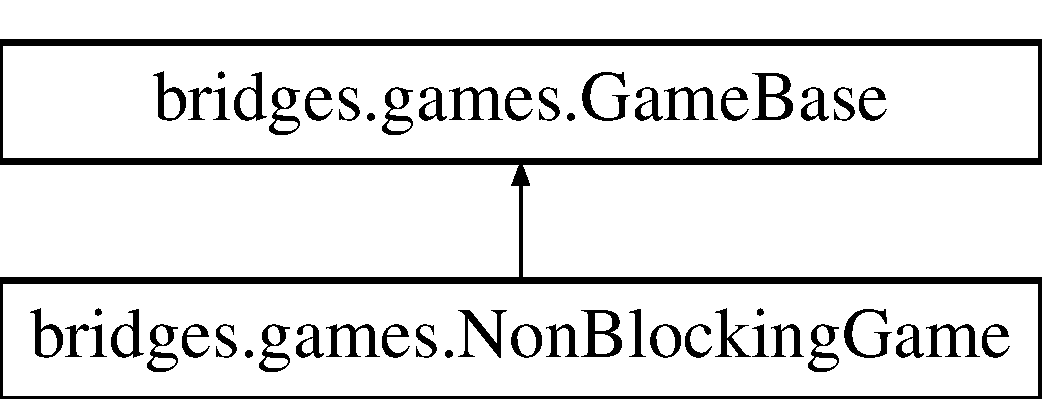
\includegraphics[height=2.000000cm]{classbridges_1_1games_1_1_non_blocking_game}
\end{center}
\end{figure}


\subsection{Detailed Description}
This class provides the features necessary to implement simple non blocking games. 

The games that can be created out of \mbox{\hyperlink{classbridges_1_1games_1_1_non_blocking_game}{Non\+Blocking\+Game}} are based on a simple board grid of at most 1024 cells (e.\+g., 32x32, or any combinations less than 1024 cells). Each cell has a background color, and a colored symbol.

This class is used by having another class derive from it and implement the two functions\+: \mbox{\hyperlink{classbridges_1_1games_1_1_game_base_a973a52d5eee7c29b01d668fba3c61657}{initialize()}} and \mbox{\hyperlink{classbridges_1_1games_1_1_game_base_a56d05ed744791cfc1c3792f39ff438f1}{game\+Loop()}}. \mbox{\hyperlink{classbridges_1_1games_1_1_game_base_a973a52d5eee7c29b01d668fba3c61657}{initialize()}} is called exactly once, on the first frame of the game. It is used to make first time initializations of the game state (such as setting the board in its initial position, for instance in chess). However, \mbox{\hyperlink{classbridges_1_1games_1_1_game_base_a56d05ed744791cfc1c3792f39ff438f1}{game\+Loop()}} is called at every frame of the game. The game starts when the function \mbox{\hyperlink{classbridges_1_1games_1_1_non_blocking_game_ac4df60691641278f139d138c7347674a}{start()}} is called on the object you created.

For this reason the simplest game that can run is created by\+:


\begin{DoxyCode}
\textcolor{keyword}{import} \mbox{\hyperlink{namespacebridges}{bridges}}.game.*;
\textcolor{keyword}{import} \mbox{\hyperlink{namespacebridges}{bridges}}.\mbox{\hyperlink{namespacebridges_1_1base}{base}}.*;
\textcolor{keyword}{class }my\_game \textcolor{keyword}{extends} \mbox{\hyperlink{classbridges_1_1games_1_1_non_blocking_game_ae85ea8dcc355372ba354f4e26323fb76}{NonBlockingGame}} \{
  \textcolor{keyword}{public} my\_game() \{ super (1, \textcolor{stringliteral}{"myuserid"},  \textcolor{stringliteral}{"myapikey"}, 10, 10); \}
  \textcolor{keyword}{public} \textcolor{keywordtype}{void} \mbox{\hyperlink{classbridges_1_1games_1_1_game_base_a973a52d5eee7c29b01d668fba3c61657}{initialize}}()  \{ \}
  \textcolor{keyword}{public} \textcolor{keywordtype}{void} \mbox{\hyperlink{classbridges_1_1games_1_1_game_base_a56d05ed744791cfc1c3792f39ff438f1}{gameLoop}}()  \{ \}
  \textcolor{keyword}{public} \textcolor{keyword}{static} \textcolor{keywordtype}{void}  main (String args[]) \{
    my\_game g = \textcolor{keyword}{new} my\_game();
    g.start();
  \}
\}
\end{DoxyCode}


This game does not do anything, but it is the minimal code that will run a game. Note that the constructor of my\+\_\+game passes 5 parameters to the constructor of \mbox{\hyperlink{classbridges_1_1games_1_1_non_blocking_game_ae85ea8dcc355372ba354f4e26323fb76}{Non\+Blocking\+Game()}}. The first three parameters are the classic parameters that the constructor of \mbox{\hyperlink{classbridges_1_1connect_1_1_bridges}{bridges.\+connect.\+Bridges}} takes (e.\+g., assignment\+ID, username, apikey), the last two are the size of the game board.

To change the board, two functions are used. \mbox{\hyperlink{classbridges_1_1games_1_1_game_base_a7b4d08cdb306a5bf7104ab5315acb414}{set\+B\+G\+Color()}} change the background color of a particular cell. It takes three parameters, the first two identify the cell of the board to change, and the last one is a color from a color palette provided by Named\+Color. \mbox{\hyperlink{classbridges_1_1games_1_1_game_base_a03e8446feb00d5957a7e160a4fa76342}{draw\+Symbol()}} takes four parameters, the first two identify the cell of the board to change, the third is a symbol from a symbol palette provided by Named\+Symbol, the fourth is the color that symbol shold be drawn in and provided by Named\+Color.

For instance, a very simple \mbox{\hyperlink{classbridges_1_1games_1_1_game_base_a973a52d5eee7c29b01d668fba3c61657}{initialize()}} could look like\+: 
\begin{DoxyCode}
\textcolor{keyword}{public} \textcolor{keywordtype}{void} \mbox{\hyperlink{classbridges_1_1games_1_1_game_base_a973a52d5eee7c29b01d668fba3c61657}{initialize}}() \{
  \mbox{\hyperlink{classbridges_1_1games_1_1_game_base_a7b4d08cdb306a5bf7104ab5315acb414}{setBGColor}}(0, 0, NamedColor.lightsalmon);
  \mbox{\hyperlink{classbridges_1_1games_1_1_game_base_a03e8446feb00d5957a7e160a4fa76342}{drawSymbol}}(0, 0, NamedSymbol.sword, NamedColor.blue);
\}
\end{DoxyCode}


Note that the size of the board was set at 10x10 and that drawing on a cell that does not exist will lead to an error. One can specify a gameboard of a different size by changing the parameters to the \mbox{\hyperlink{classbridges_1_1games_1_1_non_blocking_game}{Non\+Blocking\+Game}} constructor. However, the game board can not be more than 1024 cells in total, so a 15x15 board is possible, a 32x32 board is the largest square board possible, and a rectangular 64x16 rectangular board is also possible. But a 100x20 board would be 2000 cells and is not possible. For instance a board of 16 rows and 64 columns can be created defining the my\+\_\+game constructor as\+:


\begin{DoxyCode}
\textcolor{keyword}{public} my\_game() \{ super(1, \textcolor{stringliteral}{"myuserid"},  \textcolor{stringliteral}{"myapikey"}, 16, 64); \}
\end{DoxyCode}


The bridges game engine will call the \mbox{\hyperlink{classbridges_1_1games_1_1_game_base_a56d05ed744791cfc1c3792f39ff438f1}{game\+Loop()}} function at each frame of the game. You can write this function to modify the state of the game board using \mbox{\hyperlink{classbridges_1_1games_1_1_game_base_a7b4d08cdb306a5bf7104ab5315acb414}{set\+B\+G\+Color()}} and \mbox{\hyperlink{classbridges_1_1games_1_1_game_base_a03e8446feb00d5957a7e160a4fa76342}{draw\+Symbol()}}. For instance, the following \mbox{\hyperlink{classbridges_1_1games_1_1_game_base_a56d05ed744791cfc1c3792f39ff438f1}{game\+Loop()}} will color the board randomly one cell at a time.


\begin{DoxyCode}
\textcolor{keyword}{public} \textcolor{keywordtype}{void} \mbox{\hyperlink{classbridges_1_1games_1_1_game_base_a56d05ed744791cfc1c3792f39ff438f1}{gameLoop}}() \{
  \mbox{\hyperlink{classbridges_1_1games_1_1_game_base_a7b4d08cdb306a5bf7104ab5315acb414}{setBGColor}}(Math.random()*10, Math.random()*10, NamedColor.lightsalmon);
\}
\end{DoxyCode}


The game\+Loop can also probe the state of some keys of the keyboard using functions \mbox{\hyperlink{classbridges_1_1games_1_1_non_blocking_game_a524c340fabec1b7a69aa742e1347b7b4}{key\+Up()}}, \mbox{\hyperlink{classbridges_1_1games_1_1_non_blocking_game_ac8b9a6d6d4074105af6d28995091bd2b}{key\+Left()}}, \mbox{\hyperlink{classbridges_1_1games_1_1_non_blocking_game_ac59c5ac18a456cc1d69ec8d42a311840}{key\+Down()}}, \mbox{\hyperlink{classbridges_1_1games_1_1_non_blocking_game_a5a3db63942e995409daaf6b89f88b203}{key\+Right()}}, \mbox{\hyperlink{classbridges_1_1games_1_1_non_blocking_game_a45db18869044968a233a6f217650e34d}{key\+W()}}, \mbox{\hyperlink{classbridges_1_1games_1_1_non_blocking_game_a4328a21ca65c26e11161dfe362770917}{key\+A()}}, \mbox{\hyperlink{classbridges_1_1games_1_1_non_blocking_game_a4beb82246ef1eaf8c13aa406632ab936}{key\+S()}}, \mbox{\hyperlink{classbridges_1_1games_1_1_non_blocking_game_a830a2e8127b042f8915deb61f0038f2a}{key\+D()}}, \mbox{\hyperlink{classbridges_1_1games_1_1_non_blocking_game_a4ff32a8ba8aeb3f438751729f7380d16}{key\+Space()}}, and \mbox{\hyperlink{classbridges_1_1games_1_1_non_blocking_game_a4075b3185f2fe0d20c9ed9957c448aee}{key\+Q()}}. These functions return a boolean that indicate whether the key is pressed at that frame or not. For instance, the following code will only color the board randomly when the up arrow is pressed.


\begin{DoxyCode}
\textcolor{keyword}{public} \textcolor{keywordtype}{void} \mbox{\hyperlink{classbridges_1_1games_1_1_game_base_a56d05ed744791cfc1c3792f39ff438f1}{gameLoop}}() \{
  \textcolor{keywordflow}{if} (\mbox{\hyperlink{classbridges_1_1games_1_1_non_blocking_game_a524c340fabec1b7a69aa742e1347b7b4}{keyUp}}())
    \mbox{\hyperlink{classbridges_1_1games_1_1_game_base_a7b4d08cdb306a5bf7104ab5315acb414}{setBGColor}}(Math.random()*10, Math.rand()*10, NamedColor.lightsalmon);
\}
\end{DoxyCode}


\begin{DoxySeeAlso}{See also}
See tutorial at \href{http://bridgesuncc.github.io/tutorials/NonBlockingGame.html}{\tt http\+://bridgesuncc.\+github.\+io/tutorials/\+Non\+Blocking\+Game.\+html}
\end{DoxySeeAlso}
\begin{DoxyAuthor}{Author}
Erik Saule 
\end{DoxyAuthor}
\begin{DoxyDate}{Date}
7/21/19 
\end{DoxyDate}
\subsection*{Public Member Functions}
\begin{DoxyCompactItemize}
\item 
\mbox{\hyperlink{classbridges_1_1games_1_1_non_blocking_game_ae85ea8dcc355372ba354f4e26323fb76}{Non\+Blocking\+Game}} (int assignment\+ID, String login, String apikey, int cols, int rows)
\begin{DoxyCompactList}\small\item\em Construct a \mbox{\hyperlink{classbridges_1_1games_1_1_non_blocking_game}{Non\+Blocking\+Game}} object. It is expected students will never directly construct a \mbox{\hyperlink{classbridges_1_1games_1_1_non_blocking_game}{Non\+Blocking\+Game}} object but rather derive from it. \end{DoxyCompactList}\item 
void \mbox{\hyperlink{classbridges_1_1games_1_1_non_blocking_game_ac4df60691641278f139d138c7347674a}{start}} ()
\end{DoxyCompactItemize}
\subsection*{Protected Member Functions}
\begin{DoxyCompactItemize}
\item 
boolean \mbox{\hyperlink{classbridges_1_1games_1_1_non_blocking_game_ac8b9a6d6d4074105af6d28995091bd2b}{key\+Left}} ()
\begin{DoxyCompactList}\small\item\em Is the Left\+Arrow key currently pressed? \end{DoxyCompactList}\item 
boolean \mbox{\hyperlink{classbridges_1_1games_1_1_non_blocking_game_a5a3db63942e995409daaf6b89f88b203}{key\+Right}} ()
\begin{DoxyCompactList}\small\item\em Is the Right\+Arrow key currently pressed? \end{DoxyCompactList}\item 
boolean \mbox{\hyperlink{classbridges_1_1games_1_1_non_blocking_game_a524c340fabec1b7a69aa742e1347b7b4}{key\+Up}} ()
\begin{DoxyCompactList}\small\item\em Is the Up\+Arrow key currently pressed? \end{DoxyCompactList}\item 
boolean \mbox{\hyperlink{classbridges_1_1games_1_1_non_blocking_game_ac59c5ac18a456cc1d69ec8d42a311840}{key\+Down}} ()
\begin{DoxyCompactList}\small\item\em Is the Down\+Arrow key currently pressed? \end{DoxyCompactList}\item 
boolean \mbox{\hyperlink{classbridges_1_1games_1_1_non_blocking_game_a4075b3185f2fe0d20c9ed9957c448aee}{keyQ}} ()
\begin{DoxyCompactList}\small\item\em Is the Q key currently pressed? \end{DoxyCompactList}\item 
boolean \mbox{\hyperlink{classbridges_1_1games_1_1_non_blocking_game_a4ff32a8ba8aeb3f438751729f7380d16}{key\+Space}} ()
\begin{DoxyCompactList}\small\item\em Is the Space\+Bar key currently pressed? \end{DoxyCompactList}\item 
boolean \mbox{\hyperlink{classbridges_1_1games_1_1_non_blocking_game_a45db18869044968a233a6f217650e34d}{keyW}} ()
\begin{DoxyCompactList}\small\item\em Is the W key currently pressed? \end{DoxyCompactList}\item 
boolean \mbox{\hyperlink{classbridges_1_1games_1_1_non_blocking_game_a4328a21ca65c26e11161dfe362770917}{keyA}} ()
\begin{DoxyCompactList}\small\item\em Is the A key currently pressed? \end{DoxyCompactList}\item 
boolean \mbox{\hyperlink{classbridges_1_1games_1_1_non_blocking_game_a4beb82246ef1eaf8c13aa406632ab936}{keyS}} ()
\begin{DoxyCompactList}\small\item\em Is the S key currently pressed? \end{DoxyCompactList}\item 
boolean \mbox{\hyperlink{classbridges_1_1games_1_1_non_blocking_game_a830a2e8127b042f8915deb61f0038f2a}{keyD}} ()
\begin{DoxyCompactList}\small\item\em Is the D key currently pressed? \end{DoxyCompactList}\item 
double \mbox{\hyperlink{classbridges_1_1games_1_1_non_blocking_game_a28e91d62c0261acb7b1b0c12a9905275}{get\+Frame\+Rate}} ()
\begin{DoxyCompactList}\small\item\em What frame rate is the game running at? \end{DoxyCompactList}\end{DoxyCompactItemize}
\subsection*{Additional Inherited Members}


\subsection{Constructor \& Destructor Documentation}
\mbox{\Hypertarget{classbridges_1_1games_1_1_non_blocking_game_ae85ea8dcc355372ba354f4e26323fb76}\label{classbridges_1_1games_1_1_non_blocking_game_ae85ea8dcc355372ba354f4e26323fb76}} 
\index{bridges\+::games\+::\+Non\+Blocking\+Game@{bridges\+::games\+::\+Non\+Blocking\+Game}!Non\+Blocking\+Game@{Non\+Blocking\+Game}}
\index{Non\+Blocking\+Game@{Non\+Blocking\+Game}!bridges\+::games\+::\+Non\+Blocking\+Game@{bridges\+::games\+::\+Non\+Blocking\+Game}}
\subsubsection{\texorpdfstring{Non\+Blocking\+Game()}{NonBlockingGame()}}
{\footnotesize\ttfamily bridges.\+games.\+Non\+Blocking\+Game.\+Non\+Blocking\+Game (\begin{DoxyParamCaption}\item[{int}]{assignment\+ID,  }\item[{String}]{login,  }\item[{String}]{apikey,  }\item[{int}]{cols,  }\item[{int}]{rows }\end{DoxyParamCaption})}



Construct a \mbox{\hyperlink{classbridges_1_1games_1_1_non_blocking_game}{Non\+Blocking\+Game}} object. It is expected students will never directly construct a \mbox{\hyperlink{classbridges_1_1games_1_1_non_blocking_game}{Non\+Blocking\+Game}} object but rather derive from it. 

The created grid can not be larger than 1024 cells in total (e.\+g., 32x32, or 2x512 are ok).


\begin{DoxyParams}{Parameters}
{\em assignment\+ID} & bridges assignment ID \\
\hline
{\em login} & login on the bridges server \\
\hline
{\em apikey} & apikey of the account specified in login \\
\hline
{\em cols} & number of columns in the game \\
\hline
{\em rows} & number of rows in the game \\
\hline
\end{DoxyParams}


\subsection{Member Function Documentation}
\mbox{\Hypertarget{classbridges_1_1games_1_1_non_blocking_game_a28e91d62c0261acb7b1b0c12a9905275}\label{classbridges_1_1games_1_1_non_blocking_game_a28e91d62c0261acb7b1b0c12a9905275}} 
\index{bridges\+::games\+::\+Non\+Blocking\+Game@{bridges\+::games\+::\+Non\+Blocking\+Game}!get\+Frame\+Rate@{get\+Frame\+Rate}}
\index{get\+Frame\+Rate@{get\+Frame\+Rate}!bridges\+::games\+::\+Non\+Blocking\+Game@{bridges\+::games\+::\+Non\+Blocking\+Game}}
\subsubsection{\texorpdfstring{get\+Frame\+Rate()}{getFrameRate()}}
{\footnotesize\ttfamily double bridges.\+games.\+Non\+Blocking\+Game.\+get\+Frame\+Rate (\begin{DoxyParamCaption}{ }\end{DoxyParamCaption})\hspace{0.3cm}{\ttfamily [protected]}}



What frame rate is the game running at? 

\begin{DoxyReturn}{Returns}
the target framerate. The game could be somewhat slower depending on how computationally expensive the gameloop is and on the speed of the network. 
\end{DoxyReturn}
\mbox{\Hypertarget{classbridges_1_1games_1_1_non_blocking_game_a4328a21ca65c26e11161dfe362770917}\label{classbridges_1_1games_1_1_non_blocking_game_a4328a21ca65c26e11161dfe362770917}} 
\index{bridges\+::games\+::\+Non\+Blocking\+Game@{bridges\+::games\+::\+Non\+Blocking\+Game}!keyA@{keyA}}
\index{keyA@{keyA}!bridges\+::games\+::\+Non\+Blocking\+Game@{bridges\+::games\+::\+Non\+Blocking\+Game}}
\subsubsection{\texorpdfstring{key\+A()}{keyA()}}
{\footnotesize\ttfamily boolean bridges.\+games.\+Non\+Blocking\+Game.\+keyA (\begin{DoxyParamCaption}{ }\end{DoxyParamCaption})\hspace{0.3cm}{\ttfamily [protected]}}



Is the A key currently pressed? 

\begin{DoxyReturn}{Returns}
true if \char`\"{}a\char`\"{} is pressed? 
\end{DoxyReturn}
\mbox{\Hypertarget{classbridges_1_1games_1_1_non_blocking_game_a830a2e8127b042f8915deb61f0038f2a}\label{classbridges_1_1games_1_1_non_blocking_game_a830a2e8127b042f8915deb61f0038f2a}} 
\index{bridges\+::games\+::\+Non\+Blocking\+Game@{bridges\+::games\+::\+Non\+Blocking\+Game}!keyD@{keyD}}
\index{keyD@{keyD}!bridges\+::games\+::\+Non\+Blocking\+Game@{bridges\+::games\+::\+Non\+Blocking\+Game}}
\subsubsection{\texorpdfstring{key\+D()}{keyD()}}
{\footnotesize\ttfamily boolean bridges.\+games.\+Non\+Blocking\+Game.\+keyD (\begin{DoxyParamCaption}{ }\end{DoxyParamCaption})\hspace{0.3cm}{\ttfamily [protected]}}



Is the D key currently pressed? 

\begin{DoxyReturn}{Returns}
true if \char`\"{}d\char`\"{} is pressed 
\end{DoxyReturn}
\mbox{\Hypertarget{classbridges_1_1games_1_1_non_blocking_game_ac59c5ac18a456cc1d69ec8d42a311840}\label{classbridges_1_1games_1_1_non_blocking_game_ac59c5ac18a456cc1d69ec8d42a311840}} 
\index{bridges\+::games\+::\+Non\+Blocking\+Game@{bridges\+::games\+::\+Non\+Blocking\+Game}!key\+Down@{key\+Down}}
\index{key\+Down@{key\+Down}!bridges\+::games\+::\+Non\+Blocking\+Game@{bridges\+::games\+::\+Non\+Blocking\+Game}}
\subsubsection{\texorpdfstring{key\+Down()}{keyDown()}}
{\footnotesize\ttfamily boolean bridges.\+games.\+Non\+Blocking\+Game.\+key\+Down (\begin{DoxyParamCaption}{ }\end{DoxyParamCaption})\hspace{0.3cm}{\ttfamily [protected]}}



Is the Down\+Arrow key currently pressed? 

\begin{DoxyReturn}{Returns}
true if \char`\"{}down\char`\"{} is pressed 
\end{DoxyReturn}
\mbox{\Hypertarget{classbridges_1_1games_1_1_non_blocking_game_ac8b9a6d6d4074105af6d28995091bd2b}\label{classbridges_1_1games_1_1_non_blocking_game_ac8b9a6d6d4074105af6d28995091bd2b}} 
\index{bridges\+::games\+::\+Non\+Blocking\+Game@{bridges\+::games\+::\+Non\+Blocking\+Game}!key\+Left@{key\+Left}}
\index{key\+Left@{key\+Left}!bridges\+::games\+::\+Non\+Blocking\+Game@{bridges\+::games\+::\+Non\+Blocking\+Game}}
\subsubsection{\texorpdfstring{key\+Left()}{keyLeft()}}
{\footnotesize\ttfamily boolean bridges.\+games.\+Non\+Blocking\+Game.\+key\+Left (\begin{DoxyParamCaption}{ }\end{DoxyParamCaption})\hspace{0.3cm}{\ttfamily [protected]}}



Is the Left\+Arrow key currently pressed? 

\begin{DoxyReturn}{Returns}
true if \char`\"{}left\char`\"{} is pressed 
\end{DoxyReturn}
\mbox{\Hypertarget{classbridges_1_1games_1_1_non_blocking_game_a4075b3185f2fe0d20c9ed9957c448aee}\label{classbridges_1_1games_1_1_non_blocking_game_a4075b3185f2fe0d20c9ed9957c448aee}} 
\index{bridges\+::games\+::\+Non\+Blocking\+Game@{bridges\+::games\+::\+Non\+Blocking\+Game}!keyQ@{keyQ}}
\index{keyQ@{keyQ}!bridges\+::games\+::\+Non\+Blocking\+Game@{bridges\+::games\+::\+Non\+Blocking\+Game}}
\subsubsection{\texorpdfstring{key\+Q()}{keyQ()}}
{\footnotesize\ttfamily boolean bridges.\+games.\+Non\+Blocking\+Game.\+keyQ (\begin{DoxyParamCaption}{ }\end{DoxyParamCaption})\hspace{0.3cm}{\ttfamily [protected]}}



Is the Q key currently pressed? 

\begin{DoxyReturn}{Returns}
true if \char`\"{}q\char`\"{} is pressed 
\end{DoxyReturn}
\mbox{\Hypertarget{classbridges_1_1games_1_1_non_blocking_game_a5a3db63942e995409daaf6b89f88b203}\label{classbridges_1_1games_1_1_non_blocking_game_a5a3db63942e995409daaf6b89f88b203}} 
\index{bridges\+::games\+::\+Non\+Blocking\+Game@{bridges\+::games\+::\+Non\+Blocking\+Game}!key\+Right@{key\+Right}}
\index{key\+Right@{key\+Right}!bridges\+::games\+::\+Non\+Blocking\+Game@{bridges\+::games\+::\+Non\+Blocking\+Game}}
\subsubsection{\texorpdfstring{key\+Right()}{keyRight()}}
{\footnotesize\ttfamily boolean bridges.\+games.\+Non\+Blocking\+Game.\+key\+Right (\begin{DoxyParamCaption}{ }\end{DoxyParamCaption})\hspace{0.3cm}{\ttfamily [protected]}}



Is the Right\+Arrow key currently pressed? 

\begin{DoxyReturn}{Returns}
true if \char`\"{}right\char`\"{} is pressed 
\end{DoxyReturn}
\mbox{\Hypertarget{classbridges_1_1games_1_1_non_blocking_game_a4beb82246ef1eaf8c13aa406632ab936}\label{classbridges_1_1games_1_1_non_blocking_game_a4beb82246ef1eaf8c13aa406632ab936}} 
\index{bridges\+::games\+::\+Non\+Blocking\+Game@{bridges\+::games\+::\+Non\+Blocking\+Game}!keyS@{keyS}}
\index{keyS@{keyS}!bridges\+::games\+::\+Non\+Blocking\+Game@{bridges\+::games\+::\+Non\+Blocking\+Game}}
\subsubsection{\texorpdfstring{key\+S()}{keyS()}}
{\footnotesize\ttfamily boolean bridges.\+games.\+Non\+Blocking\+Game.\+keyS (\begin{DoxyParamCaption}{ }\end{DoxyParamCaption})\hspace{0.3cm}{\ttfamily [protected]}}



Is the S key currently pressed? 

\begin{DoxyReturn}{Returns}
true if \char`\"{}s\char`\"{} is pressed 
\end{DoxyReturn}
\mbox{\Hypertarget{classbridges_1_1games_1_1_non_blocking_game_a4ff32a8ba8aeb3f438751729f7380d16}\label{classbridges_1_1games_1_1_non_blocking_game_a4ff32a8ba8aeb3f438751729f7380d16}} 
\index{bridges\+::games\+::\+Non\+Blocking\+Game@{bridges\+::games\+::\+Non\+Blocking\+Game}!key\+Space@{key\+Space}}
\index{key\+Space@{key\+Space}!bridges\+::games\+::\+Non\+Blocking\+Game@{bridges\+::games\+::\+Non\+Blocking\+Game}}
\subsubsection{\texorpdfstring{key\+Space()}{keySpace()}}
{\footnotesize\ttfamily boolean bridges.\+games.\+Non\+Blocking\+Game.\+key\+Space (\begin{DoxyParamCaption}{ }\end{DoxyParamCaption})\hspace{0.3cm}{\ttfamily [protected]}}



Is the Space\+Bar key currently pressed? 

\begin{DoxyReturn}{Returns}
true if Space\+Bar is pressed 
\end{DoxyReturn}
\mbox{\Hypertarget{classbridges_1_1games_1_1_non_blocking_game_a524c340fabec1b7a69aa742e1347b7b4}\label{classbridges_1_1games_1_1_non_blocking_game_a524c340fabec1b7a69aa742e1347b7b4}} 
\index{bridges\+::games\+::\+Non\+Blocking\+Game@{bridges\+::games\+::\+Non\+Blocking\+Game}!key\+Up@{key\+Up}}
\index{key\+Up@{key\+Up}!bridges\+::games\+::\+Non\+Blocking\+Game@{bridges\+::games\+::\+Non\+Blocking\+Game}}
\subsubsection{\texorpdfstring{key\+Up()}{keyUp()}}
{\footnotesize\ttfamily boolean bridges.\+games.\+Non\+Blocking\+Game.\+key\+Up (\begin{DoxyParamCaption}{ }\end{DoxyParamCaption})\hspace{0.3cm}{\ttfamily [protected]}}



Is the Up\+Arrow key currently pressed? 

\begin{DoxyReturn}{Returns}
true if \char`\"{}up\char`\"{} is pressed 
\end{DoxyReturn}
\mbox{\Hypertarget{classbridges_1_1games_1_1_non_blocking_game_a45db18869044968a233a6f217650e34d}\label{classbridges_1_1games_1_1_non_blocking_game_a45db18869044968a233a6f217650e34d}} 
\index{bridges\+::games\+::\+Non\+Blocking\+Game@{bridges\+::games\+::\+Non\+Blocking\+Game}!keyW@{keyW}}
\index{keyW@{keyW}!bridges\+::games\+::\+Non\+Blocking\+Game@{bridges\+::games\+::\+Non\+Blocking\+Game}}
\subsubsection{\texorpdfstring{key\+W()}{keyW()}}
{\footnotesize\ttfamily boolean bridges.\+games.\+Non\+Blocking\+Game.\+keyW (\begin{DoxyParamCaption}{ }\end{DoxyParamCaption})\hspace{0.3cm}{\ttfamily [protected]}}



Is the W key currently pressed? 

\begin{DoxyReturn}{Returns}
true if \char`\"{}w\char`\"{} is pressed 
\end{DoxyReturn}
\mbox{\Hypertarget{classbridges_1_1games_1_1_non_blocking_game_ac4df60691641278f139d138c7347674a}\label{classbridges_1_1games_1_1_non_blocking_game_ac4df60691641278f139d138c7347674a}} 
\index{bridges\+::games\+::\+Non\+Blocking\+Game@{bridges\+::games\+::\+Non\+Blocking\+Game}!start@{start}}
\index{start@{start}!bridges\+::games\+::\+Non\+Blocking\+Game@{bridges\+::games\+::\+Non\+Blocking\+Game}}
\subsubsection{\texorpdfstring{start()}{start()}}
{\footnotesize\ttfamily void bridges.\+games.\+Non\+Blocking\+Game.\+start (\begin{DoxyParamCaption}{ }\end{DoxyParamCaption})}

Call this function to start the game engine. 

The documentation for this class was generated from the following file\+:\begin{DoxyCompactItemize}
\item 
/\+Users/kalpathi/gr/bridges/client/java/src/main/java/bridges/games/\mbox{\hyperlink{_non_blocking_game_8java}{Non\+Blocking\+Game.\+java}}\end{DoxyCompactItemize}

\hypertarget{classbridges_1_1data__src__dependent_1_1_osm_data}{}\section{bridges.\+data\+\_\+src\+\_\+dependent.\+Osm\+Data Class Reference}
\label{classbridges_1_1data__src__dependent_1_1_osm_data}\index{bridges.\+data\+\_\+src\+\_\+dependent.\+Osm\+Data@{bridges.\+data\+\_\+src\+\_\+dependent.\+Osm\+Data}}


\subsection{Detailed Description}
Class that hold Open Street Map vertices. 

This class holds Open Street Map data, from \href{https://openstreetmap.org}{\tt https\+://openstreetmap.\+org}

\begin{DoxyAuthor}{Author}
Kalpathi Subramanian, Erik Saule
\end{DoxyAuthor}
\begin{DoxyDate}{Date}
2/16/19, 12/26/20 
\end{DoxyDate}
\subsection*{Public Member Functions}
\begin{DoxyCompactItemize}
\item 
\hyperlink{classbridges_1_1data__src__dependent_1_1_osm_data_a1ba678dfedee33772a620d678f7a04d8}{Osm\+Data} ()
\item 
\hyperlink{classbridges_1_1data__src__dependent_1_1_osm_data_a822667d3269b059bf14e80c36b12fbb9}{Osm\+Data} (\hyperlink{classbridges_1_1data__src__dependent_1_1_osm_vertex}{Osm\+Vertex}\mbox{[}$\,$\mbox{]} vertices, \hyperlink{classbridges_1_1data__src__dependent_1_1_osm_edge}{Osm\+Edge}\mbox{[}$\,$\mbox{]} edges, String name)
\item 
\hyperlink{classbridges_1_1data__src__dependent_1_1_osm_vertex}{Osm\+Vertex} \mbox{[}$\,$\mbox{]} \hyperlink{classbridges_1_1data__src__dependent_1_1_osm_data_a4dc0a205132f1143e628398e08057362}{get\+Vertices} ()
\item 
void \hyperlink{classbridges_1_1data__src__dependent_1_1_osm_data_ad31b467d79dd0b76f75f93b5e192e1e3}{set\+Vertices} (\hyperlink{classbridges_1_1data__src__dependent_1_1_osm_vertex}{Osm\+Vertex}\mbox{[}$\,$\mbox{]} vertices)
\item 
String \hyperlink{classbridges_1_1data__src__dependent_1_1_osm_data_ab239e638adb7cd65a3fc7e735f6d1e61}{get\+Name} ()
\item 
void \hyperlink{classbridges_1_1data__src__dependent_1_1_osm_data_abdc3131be4ca17fcf53a5728a7932bda}{set\+Name} (String name)
\item 
\hyperlink{classbridges_1_1data__src__dependent_1_1_osm_edge}{Osm\+Edge} \mbox{[}$\,$\mbox{]} \hyperlink{classbridges_1_1data__src__dependent_1_1_osm_data_a1ceb1a4b7acd75ca655ad0769f6b427d}{get\+Edges} ()
\item 
void \hyperlink{classbridges_1_1data__src__dependent_1_1_osm_data_a88cf686718bcd27a82e2c8fb74b649f2}{set\+Edges} (\hyperlink{classbridges_1_1data__src__dependent_1_1_osm_edge}{Osm\+Edge}\mbox{[}$\,$\mbox{]} edges)
\item 
double \mbox{[}$\,$\mbox{]} \hyperlink{classbridges_1_1data__src__dependent_1_1_osm_data_a66e066ca35c27f82190e94e6c530d635}{get\+Cartesian\+RangeY} ()
\item 
double \mbox{[}$\,$\mbox{]} \hyperlink{classbridges_1_1data__src__dependent_1_1_osm_data_a406042fe56541f04c059a1f1ec887c81}{get\+Latitude\+Range} ()
\item 
double \mbox{[}$\,$\mbox{]} \hyperlink{classbridges_1_1data__src__dependent_1_1_osm_data_a4a30fc62901cd0cea50d2e4a266c6c05}{get\+Longitude\+Range} ()
\item 
double \mbox{[}$\,$\mbox{]} \hyperlink{classbridges_1_1data__src__dependent_1_1_osm_data_aa8a436daa0df5d64bc24f45b371872c5}{get\+Cartesian\+RangeX} ()
\item 
void \hyperlink{classbridges_1_1data__src__dependent_1_1_osm_data_a2f80de5c73dd1bf72378e6a0573ba663}{get\+Lat\+Long\+Range} (double\mbox{[}$\,$\mbox{]} latr, double\mbox{[}$\,$\mbox{]} lonr)
\item 
\hyperlink{classbridges_1_1base_1_1_graph_adj_list}{Graph\+Adj\+List}$<$ Integer, \hyperlink{classbridges_1_1data__src__dependent_1_1_osm_vertex}{Osm\+Vertex}, Double $>$ \hyperlink{classbridges_1_1data__src__dependent_1_1_osm_data_a4f5282b7b11ef6e4a248a05c35fe3787}{get\+Graph} ()
\end{DoxyCompactItemize}


\subsection{Constructor \& Destructor Documentation}
\mbox{\Hypertarget{classbridges_1_1data__src__dependent_1_1_osm_data_a1ba678dfedee33772a620d678f7a04d8}\label{classbridges_1_1data__src__dependent_1_1_osm_data_a1ba678dfedee33772a620d678f7a04d8}} 
\index{bridges\+::data\+\_\+src\+\_\+dependent\+::\+Osm\+Data@{bridges\+::data\+\_\+src\+\_\+dependent\+::\+Osm\+Data}!Osm\+Data@{Osm\+Data}}
\index{Osm\+Data@{Osm\+Data}!bridges\+::data\+\_\+src\+\_\+dependent\+::\+Osm\+Data@{bridges\+::data\+\_\+src\+\_\+dependent\+::\+Osm\+Data}}
\subsubsection{\texorpdfstring{Osm\+Data()}{OsmData()}\hspace{0.1cm}{\footnotesize\ttfamily [1/2]}}
{\footnotesize\ttfamily bridges.\+data\+\_\+src\+\_\+dependent.\+Osm\+Data.\+Osm\+Data (\begin{DoxyParamCaption}{ }\end{DoxyParamCaption})}

\mbox{\Hypertarget{classbridges_1_1data__src__dependent_1_1_osm_data_a822667d3269b059bf14e80c36b12fbb9}\label{classbridges_1_1data__src__dependent_1_1_osm_data_a822667d3269b059bf14e80c36b12fbb9}} 
\index{bridges\+::data\+\_\+src\+\_\+dependent\+::\+Osm\+Data@{bridges\+::data\+\_\+src\+\_\+dependent\+::\+Osm\+Data}!Osm\+Data@{Osm\+Data}}
\index{Osm\+Data@{Osm\+Data}!bridges\+::data\+\_\+src\+\_\+dependent\+::\+Osm\+Data@{bridges\+::data\+\_\+src\+\_\+dependent\+::\+Osm\+Data}}
\subsubsection{\texorpdfstring{Osm\+Data()}{OsmData()}\hspace{0.1cm}{\footnotesize\ttfamily [2/2]}}
{\footnotesize\ttfamily bridges.\+data\+\_\+src\+\_\+dependent.\+Osm\+Data.\+Osm\+Data (\begin{DoxyParamCaption}\item[{\hyperlink{classbridges_1_1data__src__dependent_1_1_osm_vertex}{Osm\+Vertex} \mbox{[}$\,$\mbox{]}}]{vertices,  }\item[{\hyperlink{classbridges_1_1data__src__dependent_1_1_osm_edge}{Osm\+Edge} \mbox{[}$\,$\mbox{]}}]{edges,  }\item[{String}]{name }\end{DoxyParamCaption})}

Constructor 
\begin{DoxyParams}{Parameters}
{\em vertices} & nodes of the map (array of \hyperlink{classbridges_1_1data__src__dependent_1_1_osm_vertex}{Osm\+Vertex}) \\
\hline
{\em edges} & links between nodes (array of \hyperlink{classbridges_1_1data__src__dependent_1_1_osm_edge}{Osm\+Edge}) \\
\hline
{\em name} & dataset name (string) \\
\hline
\end{DoxyParams}


\subsection{Member Function Documentation}
\mbox{\Hypertarget{classbridges_1_1data__src__dependent_1_1_osm_data_aa8a436daa0df5d64bc24f45b371872c5}\label{classbridges_1_1data__src__dependent_1_1_osm_data_aa8a436daa0df5d64bc24f45b371872c5}} 
\index{bridges\+::data\+\_\+src\+\_\+dependent\+::\+Osm\+Data@{bridges\+::data\+\_\+src\+\_\+dependent\+::\+Osm\+Data}!get\+Cartesian\+RangeX@{get\+Cartesian\+RangeX}}
\index{get\+Cartesian\+RangeX@{get\+Cartesian\+RangeX}!bridges\+::data\+\_\+src\+\_\+dependent\+::\+Osm\+Data@{bridges\+::data\+\_\+src\+\_\+dependent\+::\+Osm\+Data}}
\subsubsection{\texorpdfstring{get\+Cartesian\+Range\+X()}{getCartesianRangeX()}}
{\footnotesize\ttfamily double \mbox{[}$\,$\mbox{]} bridges.\+data\+\_\+src\+\_\+dependent.\+Osm\+Data.\+get\+Cartesian\+RangeX (\begin{DoxyParamCaption}{ }\end{DoxyParamCaption})}

get range of the x cartesian coordinates of vertex locations \begin{DoxyReturn}{Returns}
double\mbox{[}\mbox{]}\+: \{min\+\_\+x, max\+\_\+x\} 
\end{DoxyReturn}
\mbox{\Hypertarget{classbridges_1_1data__src__dependent_1_1_osm_data_a66e066ca35c27f82190e94e6c530d635}\label{classbridges_1_1data__src__dependent_1_1_osm_data_a66e066ca35c27f82190e94e6c530d635}} 
\index{bridges\+::data\+\_\+src\+\_\+dependent\+::\+Osm\+Data@{bridges\+::data\+\_\+src\+\_\+dependent\+::\+Osm\+Data}!get\+Cartesian\+RangeY@{get\+Cartesian\+RangeY}}
\index{get\+Cartesian\+RangeY@{get\+Cartesian\+RangeY}!bridges\+::data\+\_\+src\+\_\+dependent\+::\+Osm\+Data@{bridges\+::data\+\_\+src\+\_\+dependent\+::\+Osm\+Data}}
\subsubsection{\texorpdfstring{get\+Cartesian\+Range\+Y()}{getCartesianRangeY()}}
{\footnotesize\ttfamily double \mbox{[}$\,$\mbox{]} bridges.\+data\+\_\+src\+\_\+dependent.\+Osm\+Data.\+get\+Cartesian\+RangeY (\begin{DoxyParamCaption}{ }\end{DoxyParamCaption})}

get range of the y cartesian coordinates of vertex locations \begin{DoxyReturn}{Returns}
double\mbox{[}\mbox{]}\+: \{min\+\_\+y, max\+\_\+y\} 
\end{DoxyReturn}
\mbox{\Hypertarget{classbridges_1_1data__src__dependent_1_1_osm_data_a1ceb1a4b7acd75ca655ad0769f6b427d}\label{classbridges_1_1data__src__dependent_1_1_osm_data_a1ceb1a4b7acd75ca655ad0769f6b427d}} 
\index{bridges\+::data\+\_\+src\+\_\+dependent\+::\+Osm\+Data@{bridges\+::data\+\_\+src\+\_\+dependent\+::\+Osm\+Data}!get\+Edges@{get\+Edges}}
\index{get\+Edges@{get\+Edges}!bridges\+::data\+\_\+src\+\_\+dependent\+::\+Osm\+Data@{bridges\+::data\+\_\+src\+\_\+dependent\+::\+Osm\+Data}}
\subsubsection{\texorpdfstring{get\+Edges()}{getEdges()}}
{\footnotesize\ttfamily \hyperlink{classbridges_1_1data__src__dependent_1_1_osm_edge}{Osm\+Edge} \mbox{[}$\,$\mbox{]} bridges.\+data\+\_\+src\+\_\+dependent.\+Osm\+Data.\+get\+Edges (\begin{DoxyParamCaption}{ }\end{DoxyParamCaption})}

get edges of \hyperlink{classbridges_1_1data__src__dependent_1_1_osm_data}{Osm\+Data} \begin{DoxyReturn}{Returns}
edges\+: \hyperlink{classbridges_1_1data__src__dependent_1_1_osm_edge}{Osm\+Edge}\mbox{[}\mbox{]} 
\end{DoxyReturn}
\mbox{\Hypertarget{classbridges_1_1data__src__dependent_1_1_osm_data_a4f5282b7b11ef6e4a248a05c35fe3787}\label{classbridges_1_1data__src__dependent_1_1_osm_data_a4f5282b7b11ef6e4a248a05c35fe3787}} 
\index{bridges\+::data\+\_\+src\+\_\+dependent\+::\+Osm\+Data@{bridges\+::data\+\_\+src\+\_\+dependent\+::\+Osm\+Data}!get\+Graph@{get\+Graph}}
\index{get\+Graph@{get\+Graph}!bridges\+::data\+\_\+src\+\_\+dependent\+::\+Osm\+Data@{bridges\+::data\+\_\+src\+\_\+dependent\+::\+Osm\+Data}}
\subsubsection{\texorpdfstring{get\+Graph()}{getGraph()}}
{\footnotesize\ttfamily \hyperlink{classbridges_1_1base_1_1_graph_adj_list}{Graph\+Adj\+List}$<$Integer, \hyperlink{classbridges_1_1data__src__dependent_1_1_osm_vertex}{Osm\+Vertex}, Double$>$ bridges.\+data\+\_\+src\+\_\+dependent.\+Osm\+Data.\+get\+Graph (\begin{DoxyParamCaption}{ }\end{DoxyParamCaption})}

Construct a graph out of the vertex and edge data of the O\+SM object. The graph will associate the length of the edge to the graph edge. No data is bound to the vertices.

The vertices of the graph will be located at the location given in the data set converted to cartesian coordinate. \mbox{\Hypertarget{classbridges_1_1data__src__dependent_1_1_osm_data_a406042fe56541f04c059a1f1ec887c81}\label{classbridges_1_1data__src__dependent_1_1_osm_data_a406042fe56541f04c059a1f1ec887c81}} 
\index{bridges\+::data\+\_\+src\+\_\+dependent\+::\+Osm\+Data@{bridges\+::data\+\_\+src\+\_\+dependent\+::\+Osm\+Data}!get\+Latitude\+Range@{get\+Latitude\+Range}}
\index{get\+Latitude\+Range@{get\+Latitude\+Range}!bridges\+::data\+\_\+src\+\_\+dependent\+::\+Osm\+Data@{bridges\+::data\+\_\+src\+\_\+dependent\+::\+Osm\+Data}}
\subsubsection{\texorpdfstring{get\+Latitude\+Range()}{getLatitudeRange()}}
{\footnotesize\ttfamily double \mbox{[}$\,$\mbox{]} bridges.\+data\+\_\+src\+\_\+dependent.\+Osm\+Data.\+get\+Latitude\+Range (\begin{DoxyParamCaption}{ }\end{DoxyParamCaption})}

get range of the latitude of vertex locations \begin{DoxyReturn}{Returns}
double\mbox{[}\mbox{]}\+: \{min\+\_\+latitude, max\+\_\+latitude\} 
\end{DoxyReturn}
\mbox{\Hypertarget{classbridges_1_1data__src__dependent_1_1_osm_data_a2f80de5c73dd1bf72378e6a0573ba663}\label{classbridges_1_1data__src__dependent_1_1_osm_data_a2f80de5c73dd1bf72378e6a0573ba663}} 
\index{bridges\+::data\+\_\+src\+\_\+dependent\+::\+Osm\+Data@{bridges\+::data\+\_\+src\+\_\+dependent\+::\+Osm\+Data}!get\+Lat\+Long\+Range@{get\+Lat\+Long\+Range}}
\index{get\+Lat\+Long\+Range@{get\+Lat\+Long\+Range}!bridges\+::data\+\_\+src\+\_\+dependent\+::\+Osm\+Data@{bridges\+::data\+\_\+src\+\_\+dependent\+::\+Osm\+Data}}
\subsubsection{\texorpdfstring{get\+Lat\+Long\+Range()}{getLatLongRange()}}
{\footnotesize\ttfamily void bridges.\+data\+\_\+src\+\_\+dependent.\+Osm\+Data.\+get\+Lat\+Long\+Range (\begin{DoxyParamCaption}\item[{double \mbox{[}$\,$\mbox{]}}]{latr,  }\item[{double \mbox{[}$\,$\mbox{]}}]{lonr }\end{DoxyParamCaption})}

get the range of dataset in Cartesian coords


\begin{DoxyParams}{Parameters}
{\em latr} & double\mbox{[}2\mbox{]} \\
\hline
{\em lonr} & double\mbox{[}2\mbox{]} \\
\hline
\end{DoxyParams}
\begin{DoxyReturn}{Returns}
none 
\end{DoxyReturn}
\mbox{\Hypertarget{classbridges_1_1data__src__dependent_1_1_osm_data_a4a30fc62901cd0cea50d2e4a266c6c05}\label{classbridges_1_1data__src__dependent_1_1_osm_data_a4a30fc62901cd0cea50d2e4a266c6c05}} 
\index{bridges\+::data\+\_\+src\+\_\+dependent\+::\+Osm\+Data@{bridges\+::data\+\_\+src\+\_\+dependent\+::\+Osm\+Data}!get\+Longitude\+Range@{get\+Longitude\+Range}}
\index{get\+Longitude\+Range@{get\+Longitude\+Range}!bridges\+::data\+\_\+src\+\_\+dependent\+::\+Osm\+Data@{bridges\+::data\+\_\+src\+\_\+dependent\+::\+Osm\+Data}}
\subsubsection{\texorpdfstring{get\+Longitude\+Range()}{getLongitudeRange()}}
{\footnotesize\ttfamily double \mbox{[}$\,$\mbox{]} bridges.\+data\+\_\+src\+\_\+dependent.\+Osm\+Data.\+get\+Longitude\+Range (\begin{DoxyParamCaption}{ }\end{DoxyParamCaption})}

get range of longitude of vertex locations \begin{DoxyReturn}{Returns}
double\mbox{[}\mbox{]}\+: \{min\+\_\+longitude, max\+\_\+longitude\} 
\end{DoxyReturn}
\mbox{\Hypertarget{classbridges_1_1data__src__dependent_1_1_osm_data_ab239e638adb7cd65a3fc7e735f6d1e61}\label{classbridges_1_1data__src__dependent_1_1_osm_data_ab239e638adb7cd65a3fc7e735f6d1e61}} 
\index{bridges\+::data\+\_\+src\+\_\+dependent\+::\+Osm\+Data@{bridges\+::data\+\_\+src\+\_\+dependent\+::\+Osm\+Data}!get\+Name@{get\+Name}}
\index{get\+Name@{get\+Name}!bridges\+::data\+\_\+src\+\_\+dependent\+::\+Osm\+Data@{bridges\+::data\+\_\+src\+\_\+dependent\+::\+Osm\+Data}}
\subsubsection{\texorpdfstring{get\+Name()}{getName()}}
{\footnotesize\ttfamily String bridges.\+data\+\_\+src\+\_\+dependent.\+Osm\+Data.\+get\+Name (\begin{DoxyParamCaption}{ }\end{DoxyParamCaption})}

get name of \hyperlink{classbridges_1_1data__src__dependent_1_1_osm_data}{Osm\+Data} \begin{DoxyReturn}{Returns}
String 
\end{DoxyReturn}
\mbox{\Hypertarget{classbridges_1_1data__src__dependent_1_1_osm_data_a4dc0a205132f1143e628398e08057362}\label{classbridges_1_1data__src__dependent_1_1_osm_data_a4dc0a205132f1143e628398e08057362}} 
\index{bridges\+::data\+\_\+src\+\_\+dependent\+::\+Osm\+Data@{bridges\+::data\+\_\+src\+\_\+dependent\+::\+Osm\+Data}!get\+Vertices@{get\+Vertices}}
\index{get\+Vertices@{get\+Vertices}!bridges\+::data\+\_\+src\+\_\+dependent\+::\+Osm\+Data@{bridges\+::data\+\_\+src\+\_\+dependent\+::\+Osm\+Data}}
\subsubsection{\texorpdfstring{get\+Vertices()}{getVertices()}}
{\footnotesize\ttfamily \hyperlink{classbridges_1_1data__src__dependent_1_1_osm_vertex}{Osm\+Vertex} \mbox{[}$\,$\mbox{]} bridges.\+data\+\_\+src\+\_\+dependent.\+Osm\+Data.\+get\+Vertices (\begin{DoxyParamCaption}{ }\end{DoxyParamCaption})}

Gets the nodes of the dataset \begin{DoxyReturn}{Returns}
the nodes of the dataset (array of \hyperlink{classbridges_1_1data__src__dependent_1_1_osm_vertex}{Osm\+Vertex}) 
\end{DoxyReturn}
\mbox{\Hypertarget{classbridges_1_1data__src__dependent_1_1_osm_data_a88cf686718bcd27a82e2c8fb74b649f2}\label{classbridges_1_1data__src__dependent_1_1_osm_data_a88cf686718bcd27a82e2c8fb74b649f2}} 
\index{bridges\+::data\+\_\+src\+\_\+dependent\+::\+Osm\+Data@{bridges\+::data\+\_\+src\+\_\+dependent\+::\+Osm\+Data}!set\+Edges@{set\+Edges}}
\index{set\+Edges@{set\+Edges}!bridges\+::data\+\_\+src\+\_\+dependent\+::\+Osm\+Data@{bridges\+::data\+\_\+src\+\_\+dependent\+::\+Osm\+Data}}
\subsubsection{\texorpdfstring{set\+Edges()}{setEdges()}}
{\footnotesize\ttfamily void bridges.\+data\+\_\+src\+\_\+dependent.\+Osm\+Data.\+set\+Edges (\begin{DoxyParamCaption}\item[{\hyperlink{classbridges_1_1data__src__dependent_1_1_osm_edge}{Osm\+Edge} \mbox{[}$\,$\mbox{]}}]{edges }\end{DoxyParamCaption})}

set edges of \hyperlink{classbridges_1_1data__src__dependent_1_1_osm_data}{Osm\+Data} 
\begin{DoxyParams}{Parameters}
{\em edges} & \hyperlink{classbridges_1_1data__src__dependent_1_1_osm_edge}{Osm\+Edge}\mbox{[}\mbox{]} \\
\hline
\end{DoxyParams}
\mbox{\Hypertarget{classbridges_1_1data__src__dependent_1_1_osm_data_abdc3131be4ca17fcf53a5728a7932bda}\label{classbridges_1_1data__src__dependent_1_1_osm_data_abdc3131be4ca17fcf53a5728a7932bda}} 
\index{bridges\+::data\+\_\+src\+\_\+dependent\+::\+Osm\+Data@{bridges\+::data\+\_\+src\+\_\+dependent\+::\+Osm\+Data}!set\+Name@{set\+Name}}
\index{set\+Name@{set\+Name}!bridges\+::data\+\_\+src\+\_\+dependent\+::\+Osm\+Data@{bridges\+::data\+\_\+src\+\_\+dependent\+::\+Osm\+Data}}
\subsubsection{\texorpdfstring{set\+Name()}{setName()}}
{\footnotesize\ttfamily void bridges.\+data\+\_\+src\+\_\+dependent.\+Osm\+Data.\+set\+Name (\begin{DoxyParamCaption}\item[{String}]{name }\end{DoxyParamCaption})}

set name of \hyperlink{classbridges_1_1data__src__dependent_1_1_osm_data}{Osm\+Data} 
\begin{DoxyParams}{Parameters}
{\em name} & String \\
\hline
\end{DoxyParams}
\mbox{\Hypertarget{classbridges_1_1data__src__dependent_1_1_osm_data_ad31b467d79dd0b76f75f93b5e192e1e3}\label{classbridges_1_1data__src__dependent_1_1_osm_data_ad31b467d79dd0b76f75f93b5e192e1e3}} 
\index{bridges\+::data\+\_\+src\+\_\+dependent\+::\+Osm\+Data@{bridges\+::data\+\_\+src\+\_\+dependent\+::\+Osm\+Data}!set\+Vertices@{set\+Vertices}}
\index{set\+Vertices@{set\+Vertices}!bridges\+::data\+\_\+src\+\_\+dependent\+::\+Osm\+Data@{bridges\+::data\+\_\+src\+\_\+dependent\+::\+Osm\+Data}}
\subsubsection{\texorpdfstring{set\+Vertices()}{setVertices()}}
{\footnotesize\ttfamily void bridges.\+data\+\_\+src\+\_\+dependent.\+Osm\+Data.\+set\+Vertices (\begin{DoxyParamCaption}\item[{\hyperlink{classbridges_1_1data__src__dependent_1_1_osm_vertex}{Osm\+Vertex} \mbox{[}$\,$\mbox{]}}]{vertices }\end{DoxyParamCaption})}

Sets the nodes of the map 
\begin{DoxyParams}{Parameters}
{\em vertices} & nodes of the map \\
\hline
\end{DoxyParams}


The documentation for this class was generated from the following file\+:\begin{DoxyCompactItemize}
\item 
/home/erik/work/bridges/bridges-\/java/src/main/java/bridges/data\+\_\+src\+\_\+dependent/\hyperlink{_osm_data_8java}{Osm\+Data.\+java}\end{DoxyCompactItemize}

\hypertarget{classbridges_1_1data__src__dependent_1_1_osm_edge}{}\section{bridges.\+data\+\_\+src\+\_\+dependent.\+Osm\+Edge Class Reference}
\label{classbridges_1_1data__src__dependent_1_1_osm_edge}\index{bridges.data\_src\_dependent.OsmEdge@{bridges.data\_src\_dependent.OsmEdge}}
\subsection*{Public Member Functions}
\begin{DoxyCompactItemize}
\item 
\mbox{\hyperlink{classbridges_1_1data__src__dependent_1_1_osm_edge_a87b1d4efb3d94d8109b18f29882475f6}{Osm\+Edge}} (int source, int destination, double distance)
\item 
int \mbox{\hyperlink{classbridges_1_1data__src__dependent_1_1_osm_edge_a4ffc915a30144db8e3c1521772a6a26d}{get\+Source}} ()
\item 
void \mbox{\hyperlink{classbridges_1_1data__src__dependent_1_1_osm_edge_aa61fb02ce746b89c26c71cd2f20053e7}{set\+Source}} (int source)
\item 
int \mbox{\hyperlink{classbridges_1_1data__src__dependent_1_1_osm_edge_a9695950217254c113eada4019d647977}{get\+Destination}} ()
\item 
void \mbox{\hyperlink{classbridges_1_1data__src__dependent_1_1_osm_edge_a0bfcd0bd6dc7a4e97a078a67e41df445}{set\+Destination}} (int destination)
\item 
double \mbox{\hyperlink{classbridges_1_1data__src__dependent_1_1_osm_edge_a0bad934b9b643d5d0e375eb4210601a5}{get\+Distance}} ()
\item 
void \mbox{\hyperlink{classbridges_1_1data__src__dependent_1_1_osm_edge_afe9d2fa452c89d08d7c1a23ff3302c62}{set\+Distance}} (double distance)
\end{DoxyCompactItemize}


\subsection{Constructor \& Destructor Documentation}
\mbox{\Hypertarget{classbridges_1_1data__src__dependent_1_1_osm_edge_a87b1d4efb3d94d8109b18f29882475f6}\label{classbridges_1_1data__src__dependent_1_1_osm_edge_a87b1d4efb3d94d8109b18f29882475f6}} 
\index{bridges.data\_src\_dependent.OsmEdge@{bridges.data\_src\_dependent.OsmEdge}!OsmEdge@{OsmEdge}}
\index{OsmEdge@{OsmEdge}!bridges.data\_src\_dependent.OsmEdge@{bridges.data\_src\_dependent.OsmEdge}}
\subsubsection{\texorpdfstring{OsmEdge()}{OsmEdge()}}
{\footnotesize\ttfamily bridges.\+data\+\_\+src\+\_\+dependent.\+Osm\+Edge.\+Osm\+Edge (\begin{DoxyParamCaption}\item[{int}]{source,  }\item[{int}]{destination,  }\item[{double}]{distance }\end{DoxyParamCaption})}

constructor for \mbox{\hyperlink{classbridges_1_1data__src__dependent_1_1_osm_edge}{Osm\+Edge}} 
\begin{DoxyParams}{Parameters}
{\em source} & int, index of source vertex \\
\hline
{\em destination} & int. index of destination vertex \\
\hline
{\em distance} & double, distance between source and destination vertices \\
\hline
\end{DoxyParams}


\subsection{Member Function Documentation}
\mbox{\Hypertarget{classbridges_1_1data__src__dependent_1_1_osm_edge_a9695950217254c113eada4019d647977}\label{classbridges_1_1data__src__dependent_1_1_osm_edge_a9695950217254c113eada4019d647977}} 
\index{bridges.data\_src\_dependent.OsmEdge@{bridges.data\_src\_dependent.OsmEdge}!getDestination@{getDestination}}
\index{getDestination@{getDestination}!bridges.data\_src\_dependent.OsmEdge@{bridges.data\_src\_dependent.OsmEdge}}
\subsubsection{\texorpdfstring{getDestination()}{getDestination()}}
{\footnotesize\ttfamily int bridges.\+data\+\_\+src\+\_\+dependent.\+Osm\+Edge.\+get\+Destination (\begin{DoxyParamCaption}{ }\end{DoxyParamCaption})}

get index of destination vertex \begin{DoxyReturn}{Returns}
int 
\end{DoxyReturn}
\mbox{\Hypertarget{classbridges_1_1data__src__dependent_1_1_osm_edge_a0bad934b9b643d5d0e375eb4210601a5}\label{classbridges_1_1data__src__dependent_1_1_osm_edge_a0bad934b9b643d5d0e375eb4210601a5}} 
\index{bridges.data\_src\_dependent.OsmEdge@{bridges.data\_src\_dependent.OsmEdge}!getDistance@{getDistance}}
\index{getDistance@{getDistance}!bridges.data\_src\_dependent.OsmEdge@{bridges.data\_src\_dependent.OsmEdge}}
\subsubsection{\texorpdfstring{getDistance()}{getDistance()}}
{\footnotesize\ttfamily double bridges.\+data\+\_\+src\+\_\+dependent.\+Osm\+Edge.\+get\+Distance (\begin{DoxyParamCaption}{ }\end{DoxyParamCaption})}

get distance between the source and destination vertices \begin{DoxyReturn}{Returns}
int 
\end{DoxyReturn}
\mbox{\Hypertarget{classbridges_1_1data__src__dependent_1_1_osm_edge_a4ffc915a30144db8e3c1521772a6a26d}\label{classbridges_1_1data__src__dependent_1_1_osm_edge_a4ffc915a30144db8e3c1521772a6a26d}} 
\index{bridges.data\_src\_dependent.OsmEdge@{bridges.data\_src\_dependent.OsmEdge}!getSource@{getSource}}
\index{getSource@{getSource}!bridges.data\_src\_dependent.OsmEdge@{bridges.data\_src\_dependent.OsmEdge}}
\subsubsection{\texorpdfstring{getSource()}{getSource()}}
{\footnotesize\ttfamily int bridges.\+data\+\_\+src\+\_\+dependent.\+Osm\+Edge.\+get\+Source (\begin{DoxyParamCaption}{ }\end{DoxyParamCaption})}

get index of source vertex \begin{DoxyReturn}{Returns}
int 
\end{DoxyReturn}
\mbox{\Hypertarget{classbridges_1_1data__src__dependent_1_1_osm_edge_a0bfcd0bd6dc7a4e97a078a67e41df445}\label{classbridges_1_1data__src__dependent_1_1_osm_edge_a0bfcd0bd6dc7a4e97a078a67e41df445}} 
\index{bridges.data\_src\_dependent.OsmEdge@{bridges.data\_src\_dependent.OsmEdge}!setDestination@{setDestination}}
\index{setDestination@{setDestination}!bridges.data\_src\_dependent.OsmEdge@{bridges.data\_src\_dependent.OsmEdge}}
\subsubsection{\texorpdfstring{setDestination()}{setDestination()}}
{\footnotesize\ttfamily void bridges.\+data\+\_\+src\+\_\+dependent.\+Osm\+Edge.\+set\+Destination (\begin{DoxyParamCaption}\item[{int}]{destination }\end{DoxyParamCaption})}

set index of destination vertex 
\begin{DoxyParams}{Parameters}
{\em destination} & int \\
\hline
\end{DoxyParams}
\mbox{\Hypertarget{classbridges_1_1data__src__dependent_1_1_osm_edge_afe9d2fa452c89d08d7c1a23ff3302c62}\label{classbridges_1_1data__src__dependent_1_1_osm_edge_afe9d2fa452c89d08d7c1a23ff3302c62}} 
\index{bridges.data\_src\_dependent.OsmEdge@{bridges.data\_src\_dependent.OsmEdge}!setDistance@{setDistance}}
\index{setDistance@{setDistance}!bridges.data\_src\_dependent.OsmEdge@{bridges.data\_src\_dependent.OsmEdge}}
\subsubsection{\texorpdfstring{setDistance()}{setDistance()}}
{\footnotesize\ttfamily void bridges.\+data\+\_\+src\+\_\+dependent.\+Osm\+Edge.\+set\+Distance (\begin{DoxyParamCaption}\item[{double}]{distance }\end{DoxyParamCaption})}

set the distance between the source and destination vertices 
\begin{DoxyParams}{Parameters}
{\em distance} & double \\
\hline
\end{DoxyParams}
\mbox{\Hypertarget{classbridges_1_1data__src__dependent_1_1_osm_edge_aa61fb02ce746b89c26c71cd2f20053e7}\label{classbridges_1_1data__src__dependent_1_1_osm_edge_aa61fb02ce746b89c26c71cd2f20053e7}} 
\index{bridges.data\_src\_dependent.OsmEdge@{bridges.data\_src\_dependent.OsmEdge}!setSource@{setSource}}
\index{setSource@{setSource}!bridges.data\_src\_dependent.OsmEdge@{bridges.data\_src\_dependent.OsmEdge}}
\subsubsection{\texorpdfstring{setSource()}{setSource()}}
{\footnotesize\ttfamily void bridges.\+data\+\_\+src\+\_\+dependent.\+Osm\+Edge.\+set\+Source (\begin{DoxyParamCaption}\item[{int}]{source }\end{DoxyParamCaption})}

set index of source vertex 
\begin{DoxyParams}{Parameters}
{\em source} & int \\
\hline
\end{DoxyParams}


The documentation for this class was generated from the following file\+:\begin{DoxyCompactItemize}
\item 
/\+Users/kalpathi/gr/bridges/java/src/main/java/bridges/data\+\_\+src\+\_\+dependent/\mbox{\hyperlink{_osm_edge_8java}{Osm\+Edge.\+java}}\end{DoxyCompactItemize}

\hypertarget{classbridges_1_1data__src__dependent_1_1_osm_server_response}{}\doxysection{bridges.\+data\+\_\+src\+\_\+dependent.\+Osm\+Server\+Response Class Reference}
\label{classbridges_1_1data__src__dependent_1_1_osm_server_response}\index{bridges.data\_src\_dependent.OsmServerResponse@{bridges.data\_src\_dependent.OsmServerResponse}}
\doxysubsection*{Public Attributes}
\begin{DoxyCompactItemize}
\item 
Double \mbox{[}$\,$\mbox{]}\mbox{[}$\,$\mbox{]} \mbox{\hyperlink{classbridges_1_1data__src__dependent_1_1_osm_server_response_a09cf784347684b5c551cb88690bd1933}{nodes}}
\item 
\mbox{\hyperlink{classbridges_1_1data__src__dependent_1_1_osm_server_response_meta}{Osm\+Server\+Response\+Meta}} \mbox{\hyperlink{classbridges_1_1data__src__dependent_1_1_osm_server_response_a52c2cacc02fde7bc2f29427c96a400f5}{meta}}
\end{DoxyCompactItemize}


\doxysubsection{Member Data Documentation}
\mbox{\Hypertarget{classbridges_1_1data__src__dependent_1_1_osm_server_response_a52c2cacc02fde7bc2f29427c96a400f5}\label{classbridges_1_1data__src__dependent_1_1_osm_server_response_a52c2cacc02fde7bc2f29427c96a400f5}} 
\index{bridges.data\_src\_dependent.OsmServerResponse@{bridges.data\_src\_dependent.OsmServerResponse}!meta@{meta}}
\index{meta@{meta}!bridges.data\_src\_dependent.OsmServerResponse@{bridges.data\_src\_dependent.OsmServerResponse}}
\doxysubsubsection{\texorpdfstring{meta}{meta}}
{\footnotesize\ttfamily \mbox{\hyperlink{classbridges_1_1data__src__dependent_1_1_osm_server_response_meta}{Osm\+Server\+Response\+Meta}} bridges.\+data\+\_\+src\+\_\+dependent.\+Osm\+Server\+Response.\+meta}

\mbox{\Hypertarget{classbridges_1_1data__src__dependent_1_1_osm_server_response_a09cf784347684b5c551cb88690bd1933}\label{classbridges_1_1data__src__dependent_1_1_osm_server_response_a09cf784347684b5c551cb88690bd1933}} 
\index{bridges.data\_src\_dependent.OsmServerResponse@{bridges.data\_src\_dependent.OsmServerResponse}!nodes@{nodes}}
\index{nodes@{nodes}!bridges.data\_src\_dependent.OsmServerResponse@{bridges.data\_src\_dependent.OsmServerResponse}}
\doxysubsubsection{\texorpdfstring{nodes}{nodes}}
{\footnotesize\ttfamily Double \mbox{[}$\,$\mbox{]}\mbox{[}$\,$\mbox{]} bridges.\+data\+\_\+src\+\_\+dependent.\+Osm\+Server\+Response.\+nodes}



The documentation for this class was generated from the following file\+:\begin{DoxyCompactItemize}
\item 
/\+Users/kalpathi/gr/bridges/client/java/src/main/java/bridges/data\+\_\+src\+\_\+dependent/\mbox{\hyperlink{_osm_server_response_8java}{Osm\+Server\+Response.\+java}}\end{DoxyCompactItemize}

\hypertarget{classbridges_1_1data__src__dependent_1_1_osm_server_response_meta}{}\section{bridges.\+data\+\_\+src\+\_\+dependent.\+Osm\+Server\+Response\+Meta Class Reference}
\label{classbridges_1_1data__src__dependent_1_1_osm_server_response_meta}\index{bridges.\+data\+\_\+src\+\_\+dependent.\+Osm\+Server\+Response\+Meta@{bridges.\+data\+\_\+src\+\_\+dependent.\+Osm\+Server\+Response\+Meta}}
\subsection*{Public Attributes}
\begin{DoxyCompactItemize}
\item 
double \mbox{\hyperlink{classbridges_1_1data__src__dependent_1_1_osm_server_response_meta_a98c390a5adf668e227a9048904ebb533}{lat\+\_\+min}}
\item 
String \mbox{\hyperlink{classbridges_1_1data__src__dependent_1_1_osm_server_response_meta_aa966c46c2ed35dfff9ac877286e0fd56}{name}}
\end{DoxyCompactItemize}


\subsection{Member Data Documentation}
\mbox{\Hypertarget{classbridges_1_1data__src__dependent_1_1_osm_server_response_meta_a98c390a5adf668e227a9048904ebb533}\label{classbridges_1_1data__src__dependent_1_1_osm_server_response_meta_a98c390a5adf668e227a9048904ebb533}} 
\index{bridges\+::data\+\_\+src\+\_\+dependent\+::\+Osm\+Server\+Response\+Meta@{bridges\+::data\+\_\+src\+\_\+dependent\+::\+Osm\+Server\+Response\+Meta}!lat\+\_\+min@{lat\+\_\+min}}
\index{lat\+\_\+min@{lat\+\_\+min}!bridges\+::data\+\_\+src\+\_\+dependent\+::\+Osm\+Server\+Response\+Meta@{bridges\+::data\+\_\+src\+\_\+dependent\+::\+Osm\+Server\+Response\+Meta}}
\subsubsection{\texorpdfstring{lat\+\_\+min}{lat\_min}}
{\footnotesize\ttfamily double bridges.\+data\+\_\+src\+\_\+dependent.\+Osm\+Server\+Response\+Meta.\+lat\+\_\+min}

\mbox{\Hypertarget{classbridges_1_1data__src__dependent_1_1_osm_server_response_meta_aa966c46c2ed35dfff9ac877286e0fd56}\label{classbridges_1_1data__src__dependent_1_1_osm_server_response_meta_aa966c46c2ed35dfff9ac877286e0fd56}} 
\index{bridges\+::data\+\_\+src\+\_\+dependent\+::\+Osm\+Server\+Response\+Meta@{bridges\+::data\+\_\+src\+\_\+dependent\+::\+Osm\+Server\+Response\+Meta}!name@{name}}
\index{name@{name}!bridges\+::data\+\_\+src\+\_\+dependent\+::\+Osm\+Server\+Response\+Meta@{bridges\+::data\+\_\+src\+\_\+dependent\+::\+Osm\+Server\+Response\+Meta}}
\subsubsection{\texorpdfstring{name}{name}}
{\footnotesize\ttfamily String bridges.\+data\+\_\+src\+\_\+dependent.\+Osm\+Server\+Response\+Meta.\+name}



The documentation for this class was generated from the following file\+:\begin{DoxyCompactItemize}
\item 
/\+Users/kalpathi/gr/bridges/client/java/src/main/java/bridges/data\+\_\+src\+\_\+dependent/\mbox{\hyperlink{_osm_server_response_meta_8java}{Osm\+Server\+Response\+Meta.\+java}}\end{DoxyCompactItemize}

\hypertarget{classbridges_1_1data__src__dependent_1_1_osm_vertex}{}\doxysection{bridges.\+data\+\_\+src\+\_\+dependent.\+Osm\+Vertex Class Reference}
\label{classbridges_1_1data__src__dependent_1_1_osm_vertex}\index{bridges.data\_src\_dependent.OsmVertex@{bridges.data\_src\_dependent.OsmVertex}}
\doxysubsection*{Public Member Functions}
\begin{DoxyCompactItemize}
\item 
\mbox{\hyperlink{classbridges_1_1data__src__dependent_1_1_osm_vertex_aa95185eb1ced2e59ebf3cf9cb64773ed}{Osm\+Vertex}} (double latitude, double longitude)
\item 
double \mbox{\hyperlink{classbridges_1_1data__src__dependent_1_1_osm_vertex_a6da7cbbd1f3d686af9974d5769d4a245}{get\+Latitude}} ()
\item 
void \mbox{\hyperlink{classbridges_1_1data__src__dependent_1_1_osm_vertex_afda8504609680c855ea81f0c679298e9}{set\+Latitude}} (double latitude)
\item 
double \mbox{\hyperlink{classbridges_1_1data__src__dependent_1_1_osm_vertex_a73ce32c2897be14aa893822ce4081f3d}{get\+Longitude}} ()
\item 
void \mbox{\hyperlink{classbridges_1_1data__src__dependent_1_1_osm_vertex_a2b4ac472641b5b206cff7db53ce3285b}{set\+Longitude}} (double longitude)
\item 
double \mbox{[}$\,$\mbox{]} \mbox{\hyperlink{classbridges_1_1data__src__dependent_1_1_osm_vertex_ab0921714d93d0fc416657e39a90c404e}{get\+Cartesian\+\_\+coord}} ()
\end{DoxyCompactItemize}


\doxysubsection{Constructor \& Destructor Documentation}
\mbox{\Hypertarget{classbridges_1_1data__src__dependent_1_1_osm_vertex_aa95185eb1ced2e59ebf3cf9cb64773ed}\label{classbridges_1_1data__src__dependent_1_1_osm_vertex_aa95185eb1ced2e59ebf3cf9cb64773ed}} 
\index{bridges.data\_src\_dependent.OsmVertex@{bridges.data\_src\_dependent.OsmVertex}!OsmVertex@{OsmVertex}}
\index{OsmVertex@{OsmVertex}!bridges.data\_src\_dependent.OsmVertex@{bridges.data\_src\_dependent.OsmVertex}}
\doxysubsubsection{\texorpdfstring{OsmVertex()}{OsmVertex()}}
{\footnotesize\ttfamily bridges.\+data\+\_\+src\+\_\+dependent.\+Osm\+Vertex.\+Osm\+Vertex (\begin{DoxyParamCaption}\item[{double}]{latitude,  }\item[{double}]{longitude }\end{DoxyParamCaption})}

constructor for \mbox{\hyperlink{classbridges_1_1data__src__dependent_1_1_osm_vertex}{Osm\+Vertex}} 
\begin{DoxyParams}{Parameters}
{\em latitude} & double, latitude of vertex \\
\hline
{\em longitude} & double, longitude of vertex \\
\hline
\end{DoxyParams}


\doxysubsection{Member Function Documentation}
\mbox{\Hypertarget{classbridges_1_1data__src__dependent_1_1_osm_vertex_ab0921714d93d0fc416657e39a90c404e}\label{classbridges_1_1data__src__dependent_1_1_osm_vertex_ab0921714d93d0fc416657e39a90c404e}} 
\index{bridges.data\_src\_dependent.OsmVertex@{bridges.data\_src\_dependent.OsmVertex}!getCartesian\_coord@{getCartesian\_coord}}
\index{getCartesian\_coord@{getCartesian\_coord}!bridges.data\_src\_dependent.OsmVertex@{bridges.data\_src\_dependent.OsmVertex}}
\doxysubsubsection{\texorpdfstring{getCartesian\_coord()}{getCartesian\_coord()}}
{\footnotesize\ttfamily double \mbox{[}$\,$\mbox{]} bridges.\+data\+\_\+src\+\_\+dependent.\+Osm\+Vertex.\+get\+Cartesian\+\_\+coord (\begin{DoxyParamCaption}{ }\end{DoxyParamCaption})}

get cartesian coordinates of vertex, translated from the latitude and longitude of the vertex. \begin{DoxyReturn}{Returns}
double\mbox{[}\mbox{]}, \{x, y\} 
\end{DoxyReturn}
\mbox{\Hypertarget{classbridges_1_1data__src__dependent_1_1_osm_vertex_a6da7cbbd1f3d686af9974d5769d4a245}\label{classbridges_1_1data__src__dependent_1_1_osm_vertex_a6da7cbbd1f3d686af9974d5769d4a245}} 
\index{bridges.data\_src\_dependent.OsmVertex@{bridges.data\_src\_dependent.OsmVertex}!getLatitude@{getLatitude}}
\index{getLatitude@{getLatitude}!bridges.data\_src\_dependent.OsmVertex@{bridges.data\_src\_dependent.OsmVertex}}
\doxysubsubsection{\texorpdfstring{getLatitude()}{getLatitude()}}
{\footnotesize\ttfamily double bridges.\+data\+\_\+src\+\_\+dependent.\+Osm\+Vertex.\+get\+Latitude (\begin{DoxyParamCaption}{ }\end{DoxyParamCaption})}

get latitude of vertex \begin{DoxyReturn}{Returns}
double 
\end{DoxyReturn}
\mbox{\Hypertarget{classbridges_1_1data__src__dependent_1_1_osm_vertex_a73ce32c2897be14aa893822ce4081f3d}\label{classbridges_1_1data__src__dependent_1_1_osm_vertex_a73ce32c2897be14aa893822ce4081f3d}} 
\index{bridges.data\_src\_dependent.OsmVertex@{bridges.data\_src\_dependent.OsmVertex}!getLongitude@{getLongitude}}
\index{getLongitude@{getLongitude}!bridges.data\_src\_dependent.OsmVertex@{bridges.data\_src\_dependent.OsmVertex}}
\doxysubsubsection{\texorpdfstring{getLongitude()}{getLongitude()}}
{\footnotesize\ttfamily double bridges.\+data\+\_\+src\+\_\+dependent.\+Osm\+Vertex.\+get\+Longitude (\begin{DoxyParamCaption}{ }\end{DoxyParamCaption})}

get longitude of vertex \begin{DoxyReturn}{Returns}
double 
\end{DoxyReturn}
\mbox{\Hypertarget{classbridges_1_1data__src__dependent_1_1_osm_vertex_afda8504609680c855ea81f0c679298e9}\label{classbridges_1_1data__src__dependent_1_1_osm_vertex_afda8504609680c855ea81f0c679298e9}} 
\index{bridges.data\_src\_dependent.OsmVertex@{bridges.data\_src\_dependent.OsmVertex}!setLatitude@{setLatitude}}
\index{setLatitude@{setLatitude}!bridges.data\_src\_dependent.OsmVertex@{bridges.data\_src\_dependent.OsmVertex}}
\doxysubsubsection{\texorpdfstring{setLatitude()}{setLatitude()}}
{\footnotesize\ttfamily void bridges.\+data\+\_\+src\+\_\+dependent.\+Osm\+Vertex.\+set\+Latitude (\begin{DoxyParamCaption}\item[{double}]{latitude }\end{DoxyParamCaption})}

set latitude of vertex 
\begin{DoxyParams}{Parameters}
{\em latitude} & double \\
\hline
\end{DoxyParams}
\mbox{\Hypertarget{classbridges_1_1data__src__dependent_1_1_osm_vertex_a2b4ac472641b5b206cff7db53ce3285b}\label{classbridges_1_1data__src__dependent_1_1_osm_vertex_a2b4ac472641b5b206cff7db53ce3285b}} 
\index{bridges.data\_src\_dependent.OsmVertex@{bridges.data\_src\_dependent.OsmVertex}!setLongitude@{setLongitude}}
\index{setLongitude@{setLongitude}!bridges.data\_src\_dependent.OsmVertex@{bridges.data\_src\_dependent.OsmVertex}}
\doxysubsubsection{\texorpdfstring{setLongitude()}{setLongitude()}}
{\footnotesize\ttfamily void bridges.\+data\+\_\+src\+\_\+dependent.\+Osm\+Vertex.\+set\+Longitude (\begin{DoxyParamCaption}\item[{double}]{longitude }\end{DoxyParamCaption})}

set longitude of vertex 
\begin{DoxyParams}{Parameters}
{\em longitude} & double \\
\hline
\end{DoxyParams}


The documentation for this class was generated from the following file\+:\begin{DoxyCompactItemize}
\item 
/\+Users/kalpathi/gr/bridges/client/java/src/main/java/bridges/data\+\_\+src\+\_\+dependent/\mbox{\hyperlink{_osm_vertex_8java}{Osm\+Vertex.\+java}}\end{DoxyCompactItemize}

\hypertarget{classbridges_1_1validation_1_1_output_log}{}\section{bridges.\+validation.\+Output\+Log Class Reference}
\label{classbridges_1_1validation_1_1_output_log}\index{bridges.\+validation.\+Output\+Log@{bridges.\+validation.\+Output\+Log}}
Inheritance diagram for bridges.\+validation.\+Output\+Log\+:\begin{figure}[H]
\begin{center}
\leavevmode
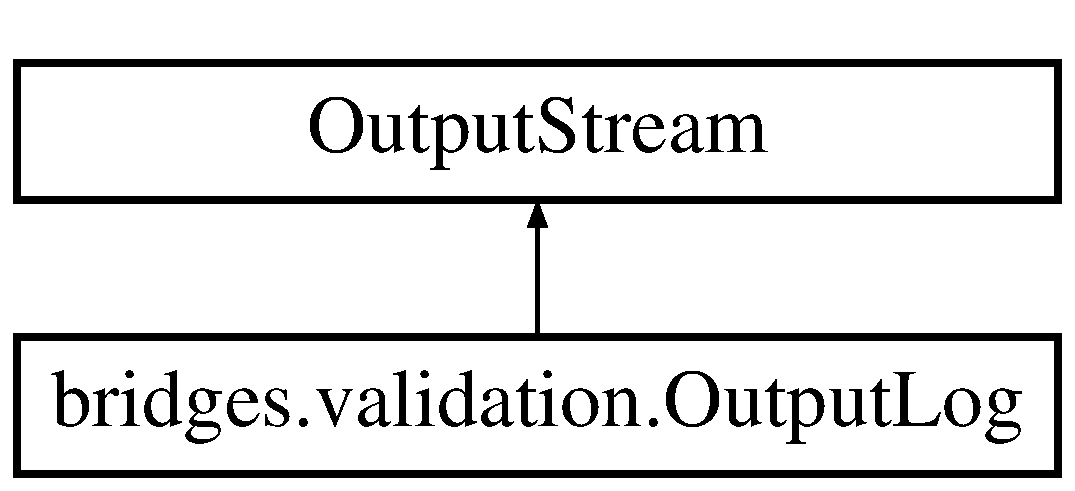
\includegraphics[height=2.000000cm]{classbridges_1_1validation_1_1_output_log}
\end{center}
\end{figure}
\subsection*{Public Member Functions}
\begin{DoxyCompactItemize}
\item 
\hyperlink{classbridges_1_1validation_1_1_output_log_a47a7efee1dce6f11f3de83d48994a56f}{Output\+Log} ()
\item 
boolean \hyperlink{classbridges_1_1validation_1_1_output_log_aae5e41b4b23adb56e3c97d2c17ad0768}{record\+Log} ()
\item 
boolean \hyperlink{classbridges_1_1validation_1_1_output_log_a4ec6037db31ff9dc0664d341183f296f}{return\+Stream} ()  throws I\+O\+Exception 
\item 
void \hyperlink{classbridges_1_1validation_1_1_output_log_a68ed2055f1a0626674675354feeb9d54}{write} (int b)  throws I\+O\+Exception 
\item 
void \hyperlink{classbridges_1_1validation_1_1_output_log_a6489f70aa4e2903456ed05315dd59f31}{write} (byte\mbox{[}$\,$\mbox{]} b)  throws I\+O\+Exception 
\item 
void \hyperlink{classbridges_1_1validation_1_1_output_log_ad0ada8f6ff72218f18b64672690fc94f}{write} (byte\mbox{[}$\,$\mbox{]} b, int a, int lenght)  throws I\+O\+Exception 
\item 
void \hyperlink{classbridges_1_1validation_1_1_output_log_a6ab7881cd35aa11cc830dab4732fe66d}{close} ()  throws I\+O\+Exception 
\item 
void \hyperlink{classbridges_1_1validation_1_1_output_log_ab810fd1e3d7e939bcdf1ec38978c02cd}{flush} ()  throws I\+O\+Exception 
\item 
void \hyperlink{classbridges_1_1validation_1_1_output_log_aea898d0de8715c1451d4731f3d9ae91d}{log\+Message} ()
\end{DoxyCompactItemize}
\subsection*{Static Public Member Functions}
\begin{DoxyCompactItemize}
\item 
static void \hyperlink{classbridges_1_1validation_1_1_output_log_a049b3ecad1138f73207d69b1193fe2e6}{split\+Stream} ()
\end{DoxyCompactItemize}
\subsection*{Static Protected Attributes}
\begin{DoxyCompactItemize}
\item 
static Print\+Stream \hyperlink{classbridges_1_1validation_1_1_output_log_a0f6ae61da2727193baf2d79a78f68614}{captured\+Stream}
\item 
static Print\+Stream \hyperlink{classbridges_1_1validation_1_1_output_log_acf8b19de1738e70f12eba5854b9e01b4}{new\+Output\+Stream}
\item 
static Print\+Stream \hyperlink{classbridges_1_1validation_1_1_output_log_a007a8494bdda0f4164663df8afe2c392}{log\+Stream}
\item 
static Print\+Stream \hyperlink{classbridges_1_1validation_1_1_output_log_a3b5198266da9d86da13fab21c096f18c}{log\+Stream2}
\item 
static File\+Output\+Stream \hyperlink{classbridges_1_1validation_1_1_output_log_a0e10e95bbb841f1f17b3b363461db3f3}{log\+File}
\item 
static Byte\+Array\+Output\+Stream \hyperlink{classbridges_1_1validation_1_1_output_log_a142611812dd1ea095c4a1274bd40a93a}{temp1}
\item 
static Byte\+Array\+Output\+Stream \hyperlink{classbridges_1_1validation_1_1_output_log_ab1f0ab7e9ada60f29c4c4f59694c1163}{temp2}
\item 
static String \hyperlink{classbridges_1_1validation_1_1_output_log_a74d7353fe97c80b3880825d18d7ccaa5}{a\+Path\+To\+Log}
\end{DoxyCompactItemize}


\subsection{Constructor \& Destructor Documentation}
\mbox{\Hypertarget{classbridges_1_1validation_1_1_output_log_a47a7efee1dce6f11f3de83d48994a56f}\label{classbridges_1_1validation_1_1_output_log_a47a7efee1dce6f11f3de83d48994a56f}} 
\index{bridges\+::validation\+::\+Output\+Log@{bridges\+::validation\+::\+Output\+Log}!Output\+Log@{Output\+Log}}
\index{Output\+Log@{Output\+Log}!bridges\+::validation\+::\+Output\+Log@{bridges\+::validation\+::\+Output\+Log}}
\subsubsection{\texorpdfstring{Output\+Log()}{OutputLog()}}
{\footnotesize\ttfamily bridges.\+validation.\+Output\+Log.\+Output\+Log (\begin{DoxyParamCaption}{ }\end{DoxyParamCaption})}

Constructor 

\subsection{Member Function Documentation}
\mbox{\Hypertarget{classbridges_1_1validation_1_1_output_log_a6ab7881cd35aa11cc830dab4732fe66d}\label{classbridges_1_1validation_1_1_output_log_a6ab7881cd35aa11cc830dab4732fe66d}} 
\index{bridges\+::validation\+::\+Output\+Log@{bridges\+::validation\+::\+Output\+Log}!close@{close}}
\index{close@{close}!bridges\+::validation\+::\+Output\+Log@{bridges\+::validation\+::\+Output\+Log}}
\subsubsection{\texorpdfstring{close()}{close()}}
{\footnotesize\ttfamily void bridges.\+validation.\+Output\+Log.\+close (\begin{DoxyParamCaption}{ }\end{DoxyParamCaption}) throws I\+O\+Exception}

\mbox{\Hypertarget{classbridges_1_1validation_1_1_output_log_ab810fd1e3d7e939bcdf1ec38978c02cd}\label{classbridges_1_1validation_1_1_output_log_ab810fd1e3d7e939bcdf1ec38978c02cd}} 
\index{bridges\+::validation\+::\+Output\+Log@{bridges\+::validation\+::\+Output\+Log}!flush@{flush}}
\index{flush@{flush}!bridges\+::validation\+::\+Output\+Log@{bridges\+::validation\+::\+Output\+Log}}
\subsubsection{\texorpdfstring{flush()}{flush()}}
{\footnotesize\ttfamily void bridges.\+validation.\+Output\+Log.\+flush (\begin{DoxyParamCaption}{ }\end{DoxyParamCaption}) throws I\+O\+Exception}

\mbox{\Hypertarget{classbridges_1_1validation_1_1_output_log_aea898d0de8715c1451d4731f3d9ae91d}\label{classbridges_1_1validation_1_1_output_log_aea898d0de8715c1451d4731f3d9ae91d}} 
\index{bridges\+::validation\+::\+Output\+Log@{bridges\+::validation\+::\+Output\+Log}!log\+Message@{log\+Message}}
\index{log\+Message@{log\+Message}!bridges\+::validation\+::\+Output\+Log@{bridges\+::validation\+::\+Output\+Log}}
\subsubsection{\texorpdfstring{log\+Message()}{logMessage()}}
{\footnotesize\ttfamily void bridges.\+validation.\+Output\+Log.\+log\+Message (\begin{DoxyParamCaption}{ }\end{DoxyParamCaption})}

This prints the Logger message to standard output \mbox{\Hypertarget{classbridges_1_1validation_1_1_output_log_aae5e41b4b23adb56e3c97d2c17ad0768}\label{classbridges_1_1validation_1_1_output_log_aae5e41b4b23adb56e3c97d2c17ad0768}} 
\index{bridges\+::validation\+::\+Output\+Log@{bridges\+::validation\+::\+Output\+Log}!record\+Log@{record\+Log}}
\index{record\+Log@{record\+Log}!bridges\+::validation\+::\+Output\+Log@{bridges\+::validation\+::\+Output\+Log}}
\subsubsection{\texorpdfstring{record\+Log()}{recordLog()}}
{\footnotesize\ttfamily boolean bridges.\+validation.\+Output\+Log.\+record\+Log (\begin{DoxyParamCaption}{ }\end{DoxyParamCaption})}

This method records the time stamp to the current log entry \begin{DoxyReturn}{Returns}
boolean 
\end{DoxyReturn}
\mbox{\Hypertarget{classbridges_1_1validation_1_1_output_log_a4ec6037db31ff9dc0664d341183f296f}\label{classbridges_1_1validation_1_1_output_log_a4ec6037db31ff9dc0664d341183f296f}} 
\index{bridges\+::validation\+::\+Output\+Log@{bridges\+::validation\+::\+Output\+Log}!return\+Stream@{return\+Stream}}
\index{return\+Stream@{return\+Stream}!bridges\+::validation\+::\+Output\+Log@{bridges\+::validation\+::\+Output\+Log}}
\subsubsection{\texorpdfstring{return\+Stream()}{returnStream()}}
{\footnotesize\ttfamily boolean bridges.\+validation.\+Output\+Log.\+return\+Stream (\begin{DoxyParamCaption}{ }\end{DoxyParamCaption}) throws I\+O\+Exception}

This method returns the stream to standard output \begin{DoxyReturn}{Returns}
boolean 
\end{DoxyReturn}
\mbox{\Hypertarget{classbridges_1_1validation_1_1_output_log_a049b3ecad1138f73207d69b1193fe2e6}\label{classbridges_1_1validation_1_1_output_log_a049b3ecad1138f73207d69b1193fe2e6}} 
\index{bridges\+::validation\+::\+Output\+Log@{bridges\+::validation\+::\+Output\+Log}!split\+Stream@{split\+Stream}}
\index{split\+Stream@{split\+Stream}!bridges\+::validation\+::\+Output\+Log@{bridges\+::validation\+::\+Output\+Log}}
\subsubsection{\texorpdfstring{split\+Stream()}{splitStream()}}
{\footnotesize\ttfamily static void bridges.\+validation.\+Output\+Log.\+split\+Stream (\begin{DoxyParamCaption}{ }\end{DoxyParamCaption})\hspace{0.3cm}{\ttfamily [static]}}

This method redirects the IO stream \mbox{\Hypertarget{classbridges_1_1validation_1_1_output_log_a68ed2055f1a0626674675354feeb9d54}\label{classbridges_1_1validation_1_1_output_log_a68ed2055f1a0626674675354feeb9d54}} 
\index{bridges\+::validation\+::\+Output\+Log@{bridges\+::validation\+::\+Output\+Log}!write@{write}}
\index{write@{write}!bridges\+::validation\+::\+Output\+Log@{bridges\+::validation\+::\+Output\+Log}}
\subsubsection{\texorpdfstring{write()}{write()}\hspace{0.1cm}{\footnotesize\ttfamily [1/3]}}
{\footnotesize\ttfamily void bridges.\+validation.\+Output\+Log.\+write (\begin{DoxyParamCaption}\item[{int}]{b }\end{DoxyParamCaption}) throws I\+O\+Exception}

\mbox{\Hypertarget{classbridges_1_1validation_1_1_output_log_a6489f70aa4e2903456ed05315dd59f31}\label{classbridges_1_1validation_1_1_output_log_a6489f70aa4e2903456ed05315dd59f31}} 
\index{bridges\+::validation\+::\+Output\+Log@{bridges\+::validation\+::\+Output\+Log}!write@{write}}
\index{write@{write}!bridges\+::validation\+::\+Output\+Log@{bridges\+::validation\+::\+Output\+Log}}
\subsubsection{\texorpdfstring{write()}{write()}\hspace{0.1cm}{\footnotesize\ttfamily [2/3]}}
{\footnotesize\ttfamily void bridges.\+validation.\+Output\+Log.\+write (\begin{DoxyParamCaption}\item[{byte \mbox{[}$\,$\mbox{]}}]{b }\end{DoxyParamCaption}) throws I\+O\+Exception}

\mbox{\Hypertarget{classbridges_1_1validation_1_1_output_log_ad0ada8f6ff72218f18b64672690fc94f}\label{classbridges_1_1validation_1_1_output_log_ad0ada8f6ff72218f18b64672690fc94f}} 
\index{bridges\+::validation\+::\+Output\+Log@{bridges\+::validation\+::\+Output\+Log}!write@{write}}
\index{write@{write}!bridges\+::validation\+::\+Output\+Log@{bridges\+::validation\+::\+Output\+Log}}
\subsubsection{\texorpdfstring{write()}{write()}\hspace{0.1cm}{\footnotesize\ttfamily [3/3]}}
{\footnotesize\ttfamily void bridges.\+validation.\+Output\+Log.\+write (\begin{DoxyParamCaption}\item[{byte \mbox{[}$\,$\mbox{]}}]{b,  }\item[{int}]{a,  }\item[{int}]{lenght }\end{DoxyParamCaption}) throws I\+O\+Exception}



\subsection{Member Data Documentation}
\mbox{\Hypertarget{classbridges_1_1validation_1_1_output_log_a74d7353fe97c80b3880825d18d7ccaa5}\label{classbridges_1_1validation_1_1_output_log_a74d7353fe97c80b3880825d18d7ccaa5}} 
\index{bridges\+::validation\+::\+Output\+Log@{bridges\+::validation\+::\+Output\+Log}!a\+Path\+To\+Log@{a\+Path\+To\+Log}}
\index{a\+Path\+To\+Log@{a\+Path\+To\+Log}!bridges\+::validation\+::\+Output\+Log@{bridges\+::validation\+::\+Output\+Log}}
\subsubsection{\texorpdfstring{a\+Path\+To\+Log}{aPathToLog}}
{\footnotesize\ttfamily String bridges.\+validation.\+Output\+Log.\+a\+Path\+To\+Log\hspace{0.3cm}{\ttfamily [static]}, {\ttfamily [protected]}}

\mbox{\Hypertarget{classbridges_1_1validation_1_1_output_log_a0f6ae61da2727193baf2d79a78f68614}\label{classbridges_1_1validation_1_1_output_log_a0f6ae61da2727193baf2d79a78f68614}} 
\index{bridges\+::validation\+::\+Output\+Log@{bridges\+::validation\+::\+Output\+Log}!captured\+Stream@{captured\+Stream}}
\index{captured\+Stream@{captured\+Stream}!bridges\+::validation\+::\+Output\+Log@{bridges\+::validation\+::\+Output\+Log}}
\subsubsection{\texorpdfstring{captured\+Stream}{capturedStream}}
{\footnotesize\ttfamily Print\+Stream bridges.\+validation.\+Output\+Log.\+captured\+Stream\hspace{0.3cm}{\ttfamily [static]}, {\ttfamily [protected]}}

\mbox{\Hypertarget{classbridges_1_1validation_1_1_output_log_a0e10e95bbb841f1f17b3b363461db3f3}\label{classbridges_1_1validation_1_1_output_log_a0e10e95bbb841f1f17b3b363461db3f3}} 
\index{bridges\+::validation\+::\+Output\+Log@{bridges\+::validation\+::\+Output\+Log}!log\+File@{log\+File}}
\index{log\+File@{log\+File}!bridges\+::validation\+::\+Output\+Log@{bridges\+::validation\+::\+Output\+Log}}
\subsubsection{\texorpdfstring{log\+File}{logFile}}
{\footnotesize\ttfamily File\+Output\+Stream bridges.\+validation.\+Output\+Log.\+log\+File\hspace{0.3cm}{\ttfamily [static]}, {\ttfamily [protected]}}

\mbox{\Hypertarget{classbridges_1_1validation_1_1_output_log_a007a8494bdda0f4164663df8afe2c392}\label{classbridges_1_1validation_1_1_output_log_a007a8494bdda0f4164663df8afe2c392}} 
\index{bridges\+::validation\+::\+Output\+Log@{bridges\+::validation\+::\+Output\+Log}!log\+Stream@{log\+Stream}}
\index{log\+Stream@{log\+Stream}!bridges\+::validation\+::\+Output\+Log@{bridges\+::validation\+::\+Output\+Log}}
\subsubsection{\texorpdfstring{log\+Stream}{logStream}}
{\footnotesize\ttfamily Print\+Stream bridges.\+validation.\+Output\+Log.\+log\+Stream\hspace{0.3cm}{\ttfamily [static]}, {\ttfamily [protected]}}

\mbox{\Hypertarget{classbridges_1_1validation_1_1_output_log_a3b5198266da9d86da13fab21c096f18c}\label{classbridges_1_1validation_1_1_output_log_a3b5198266da9d86da13fab21c096f18c}} 
\index{bridges\+::validation\+::\+Output\+Log@{bridges\+::validation\+::\+Output\+Log}!log\+Stream2@{log\+Stream2}}
\index{log\+Stream2@{log\+Stream2}!bridges\+::validation\+::\+Output\+Log@{bridges\+::validation\+::\+Output\+Log}}
\subsubsection{\texorpdfstring{log\+Stream2}{logStream2}}
{\footnotesize\ttfamily Print\+Stream bridges.\+validation.\+Output\+Log.\+log\+Stream2\hspace{0.3cm}{\ttfamily [static]}, {\ttfamily [protected]}}

\mbox{\Hypertarget{classbridges_1_1validation_1_1_output_log_acf8b19de1738e70f12eba5854b9e01b4}\label{classbridges_1_1validation_1_1_output_log_acf8b19de1738e70f12eba5854b9e01b4}} 
\index{bridges\+::validation\+::\+Output\+Log@{bridges\+::validation\+::\+Output\+Log}!new\+Output\+Stream@{new\+Output\+Stream}}
\index{new\+Output\+Stream@{new\+Output\+Stream}!bridges\+::validation\+::\+Output\+Log@{bridges\+::validation\+::\+Output\+Log}}
\subsubsection{\texorpdfstring{new\+Output\+Stream}{newOutputStream}}
{\footnotesize\ttfamily Print\+Stream bridges.\+validation.\+Output\+Log.\+new\+Output\+Stream\hspace{0.3cm}{\ttfamily [static]}, {\ttfamily [protected]}}

\mbox{\Hypertarget{classbridges_1_1validation_1_1_output_log_a142611812dd1ea095c4a1274bd40a93a}\label{classbridges_1_1validation_1_1_output_log_a142611812dd1ea095c4a1274bd40a93a}} 
\index{bridges\+::validation\+::\+Output\+Log@{bridges\+::validation\+::\+Output\+Log}!temp1@{temp1}}
\index{temp1@{temp1}!bridges\+::validation\+::\+Output\+Log@{bridges\+::validation\+::\+Output\+Log}}
\subsubsection{\texorpdfstring{temp1}{temp1}}
{\footnotesize\ttfamily Byte\+Array\+Output\+Stream bridges.\+validation.\+Output\+Log.\+temp1\hspace{0.3cm}{\ttfamily [static]}, {\ttfamily [protected]}}

\mbox{\Hypertarget{classbridges_1_1validation_1_1_output_log_ab1f0ab7e9ada60f29c4c4f59694c1163}\label{classbridges_1_1validation_1_1_output_log_ab1f0ab7e9ada60f29c4c4f59694c1163}} 
\index{bridges\+::validation\+::\+Output\+Log@{bridges\+::validation\+::\+Output\+Log}!temp2@{temp2}}
\index{temp2@{temp2}!bridges\+::validation\+::\+Output\+Log@{bridges\+::validation\+::\+Output\+Log}}
\subsubsection{\texorpdfstring{temp2}{temp2}}
{\footnotesize\ttfamily Byte\+Array\+Output\+Stream bridges.\+validation.\+Output\+Log.\+temp2\hspace{0.3cm}{\ttfamily [static]}, {\ttfamily [protected]}}



The documentation for this class was generated from the following file\+:\begin{DoxyCompactItemize}
\item 
/home/erik/work/bridges/bridges-\/java/src/main/java/bridges/validation/\hyperlink{_output_log_8java}{Output\+Log.\+java}\end{DoxyCompactItemize}

\hypertarget{classbridges_1_1benchmark_1_1_page_rank_benchmark}{}\section{bridges.\+benchmark.\+Page\+Rank\+Benchmark Class Reference}
\label{classbridges_1_1benchmark_1_1_page_rank_benchmark}\index{bridges.\+benchmark.\+Page\+Rank\+Benchmark@{bridges.\+benchmark.\+Page\+Rank\+Benchmark}}


Inherits bridges.\+benchmark.\+Graph\+Benchmark.



\subsection{Detailed Description}
Benchmarks Page Rank algorithms. 

Benchmarks Page\+Rank algorithms and add time series to a Line\+Chart.

One can also set a maximum time spent on a particular run using set\+Time\+Cap().

and can be passed to the run function for being benchmarked. A typical use would look something like


\begin{DoxyCode}
LineChart lc;
\hyperlink{classbridges_1_1benchmark_1_1_page_rank_benchmark_afd361f9cae2425b44794e2599cc25af1}{PageRankBenchmark} sb  = \textcolor{keyword}{new} \hyperlink{classbridges_1_1benchmark_1_1_page_rank_benchmark_afd361f9cae2425b44794e2599cc25af1}{PageRankBenchmark}(lc);
sb.run(\textcolor{stringliteral}{"mybfsalgorithm"}, pralgo);
\end{DoxyCode}


\begin{DoxyAuthor}{Author}
Erik Saule 
\end{DoxyAuthor}
\begin{DoxyDate}{Date}
07/21/2019 
\end{DoxyDate}
\subsection*{Public Member Functions}
\begin{DoxyCompactItemize}
\item 
\hyperlink{classbridges_1_1benchmark_1_1_page_rank_benchmark_afd361f9cae2425b44794e2599cc25af1}{Page\+Rank\+Benchmark} (\hyperlink{classbridges_1_1base_1_1_line_chart}{Line\+Chart} plot, long time\+Cap)
\item 
\hyperlink{classbridges_1_1benchmark_1_1_page_rank_benchmark_a3a74e3703d4bc24b02a9dcb59b976792}{Page\+Rank\+Benchmark} (\hyperlink{classbridges_1_1base_1_1_line_chart}{Line\+Chart} plot)
\item 
void \hyperlink{classbridges_1_1benchmark_1_1_page_rank_benchmark_a6738599d19f7a856a16615f69050c8b3}{run} (String algo\+Name, Consumer$<$ \hyperlink{classbridges_1_1benchmark_1_1_page_rank_params}{Page\+Rank\+Params} $>$ pr\+Algo)  throws I\+O\+Exception 
\end{DoxyCompactItemize}


\subsection{Constructor \& Destructor Documentation}
\mbox{\Hypertarget{classbridges_1_1benchmark_1_1_page_rank_benchmark_afd361f9cae2425b44794e2599cc25af1}\label{classbridges_1_1benchmark_1_1_page_rank_benchmark_afd361f9cae2425b44794e2599cc25af1}} 
\index{bridges\+::benchmark\+::\+Page\+Rank\+Benchmark@{bridges\+::benchmark\+::\+Page\+Rank\+Benchmark}!Page\+Rank\+Benchmark@{Page\+Rank\+Benchmark}}
\index{Page\+Rank\+Benchmark@{Page\+Rank\+Benchmark}!bridges\+::benchmark\+::\+Page\+Rank\+Benchmark@{bridges\+::benchmark\+::\+Page\+Rank\+Benchmark}}
\subsubsection{\texorpdfstring{Page\+Rank\+Benchmark()}{PageRankBenchmark()}\hspace{0.1cm}{\footnotesize\ttfamily [1/2]}}
{\footnotesize\ttfamily bridges.\+benchmark.\+Page\+Rank\+Benchmark.\+Page\+Rank\+Benchmark (\begin{DoxyParamCaption}\item[{\hyperlink{classbridges_1_1base_1_1_line_chart}{Line\+Chart}}]{plot,  }\item[{long}]{time\+Cap }\end{DoxyParamCaption})}

\mbox{\Hypertarget{classbridges_1_1benchmark_1_1_page_rank_benchmark_a3a74e3703d4bc24b02a9dcb59b976792}\label{classbridges_1_1benchmark_1_1_page_rank_benchmark_a3a74e3703d4bc24b02a9dcb59b976792}} 
\index{bridges\+::benchmark\+::\+Page\+Rank\+Benchmark@{bridges\+::benchmark\+::\+Page\+Rank\+Benchmark}!Page\+Rank\+Benchmark@{Page\+Rank\+Benchmark}}
\index{Page\+Rank\+Benchmark@{Page\+Rank\+Benchmark}!bridges\+::benchmark\+::\+Page\+Rank\+Benchmark@{bridges\+::benchmark\+::\+Page\+Rank\+Benchmark}}
\subsubsection{\texorpdfstring{Page\+Rank\+Benchmark()}{PageRankBenchmark()}\hspace{0.1cm}{\footnotesize\ttfamily [2/2]}}
{\footnotesize\ttfamily bridges.\+benchmark.\+Page\+Rank\+Benchmark.\+Page\+Rank\+Benchmark (\begin{DoxyParamCaption}\item[{\hyperlink{classbridges_1_1base_1_1_line_chart}{Line\+Chart}}]{plot }\end{DoxyParamCaption})}



\subsection{Member Function Documentation}
\mbox{\Hypertarget{classbridges_1_1benchmark_1_1_page_rank_benchmark_a6738599d19f7a856a16615f69050c8b3}\label{classbridges_1_1benchmark_1_1_page_rank_benchmark_a6738599d19f7a856a16615f69050c8b3}} 
\index{bridges\+::benchmark\+::\+Page\+Rank\+Benchmark@{bridges\+::benchmark\+::\+Page\+Rank\+Benchmark}!run@{run}}
\index{run@{run}!bridges\+::benchmark\+::\+Page\+Rank\+Benchmark@{bridges\+::benchmark\+::\+Page\+Rank\+Benchmark}}
\subsubsection{\texorpdfstring{run()}{run()}}
{\footnotesize\ttfamily void bridges.\+benchmark.\+Page\+Rank\+Benchmark.\+run (\begin{DoxyParamCaption}\item[{String}]{algo\+Name,  }\item[{Consumer$<$ \hyperlink{classbridges_1_1benchmark_1_1_page_rank_params}{Page\+Rank\+Params} $>$}]{pr\+Algo }\end{DoxyParamCaption}) throws I\+O\+Exception}



The documentation for this class was generated from the following file\+:\begin{DoxyCompactItemize}
\item 
/home/erik/work/bridges/bridges-\/java/src/main/java/bridges/benchmark/\hyperlink{_page_rank_benchmark_8java}{Page\+Rank\+Benchmark.\+java}\end{DoxyCompactItemize}

\hypertarget{classbridges_1_1benchmark_1_1_page_rank_params}{}\section{bridges.\+benchmark.\+Page\+Rank\+Params Class Reference}
\label{classbridges_1_1benchmark_1_1_page_rank_params}\index{bridges.\+benchmark.\+Page\+Rank\+Params@{bridges.\+benchmark.\+Page\+Rank\+Params}}


Inherits bridges.\+benchmark.\+Benchmark\+Params.

\subsection*{Public Attributes}
\begin{DoxyCompactItemize}
\item 
\hyperlink{classbridges_1_1base_1_1_graph_adj_list}{Graph\+Adj\+List}$<$ String, String, String $>$ \hyperlink{classbridges_1_1benchmark_1_1_page_rank_params_a5356d0005805dc3a9749e6e7a2659c49}{graph}
\item 
Hash\+Map$<$ String, Double $>$ \hyperlink{classbridges_1_1benchmark_1_1_page_rank_params_aaf852c1fecafa8ed2d222edea9246f7a}{page\+Rank}
\end{DoxyCompactItemize}


\subsection{Member Data Documentation}
\mbox{\Hypertarget{classbridges_1_1benchmark_1_1_page_rank_params_a5356d0005805dc3a9749e6e7a2659c49}\label{classbridges_1_1benchmark_1_1_page_rank_params_a5356d0005805dc3a9749e6e7a2659c49}} 
\index{bridges\+::benchmark\+::\+Page\+Rank\+Params@{bridges\+::benchmark\+::\+Page\+Rank\+Params}!graph@{graph}}
\index{graph@{graph}!bridges\+::benchmark\+::\+Page\+Rank\+Params@{bridges\+::benchmark\+::\+Page\+Rank\+Params}}
\subsubsection{\texorpdfstring{graph}{graph}}
{\footnotesize\ttfamily \hyperlink{classbridges_1_1base_1_1_graph_adj_list}{Graph\+Adj\+List}$<$String, String, String$>$ bridges.\+benchmark.\+Page\+Rank\+Params.\+graph}

\mbox{\Hypertarget{classbridges_1_1benchmark_1_1_page_rank_params_aaf852c1fecafa8ed2d222edea9246f7a}\label{classbridges_1_1benchmark_1_1_page_rank_params_aaf852c1fecafa8ed2d222edea9246f7a}} 
\index{bridges\+::benchmark\+::\+Page\+Rank\+Params@{bridges\+::benchmark\+::\+Page\+Rank\+Params}!page\+Rank@{page\+Rank}}
\index{page\+Rank@{page\+Rank}!bridges\+::benchmark\+::\+Page\+Rank\+Params@{bridges\+::benchmark\+::\+Page\+Rank\+Params}}
\subsubsection{\texorpdfstring{page\+Rank}{pageRank}}
{\footnotesize\ttfamily Hash\+Map$<$String, Double$>$ bridges.\+benchmark.\+Page\+Rank\+Params.\+page\+Rank}



The documentation for this class was generated from the following file\+:\begin{DoxyCompactItemize}
\item 
/home/erik/work/bridges/bridges-\/java/src/main/java/bridges/benchmark/\hyperlink{_page_rank_params_8java}{Page\+Rank\+Params.\+java}\end{DoxyCompactItemize}

\hypertarget{classbridges_1_1base_1_1_polygon}{}\section{bridges.\+base.\+Polygon Class Reference}
\label{classbridges_1_1base_1_1_polygon}\index{bridges.\+base.\+Polygon@{bridges.\+base.\+Polygon}}
Inheritance diagram for bridges.\+base.\+Polygon\+:\begin{figure}[H]
\begin{center}
\leavevmode
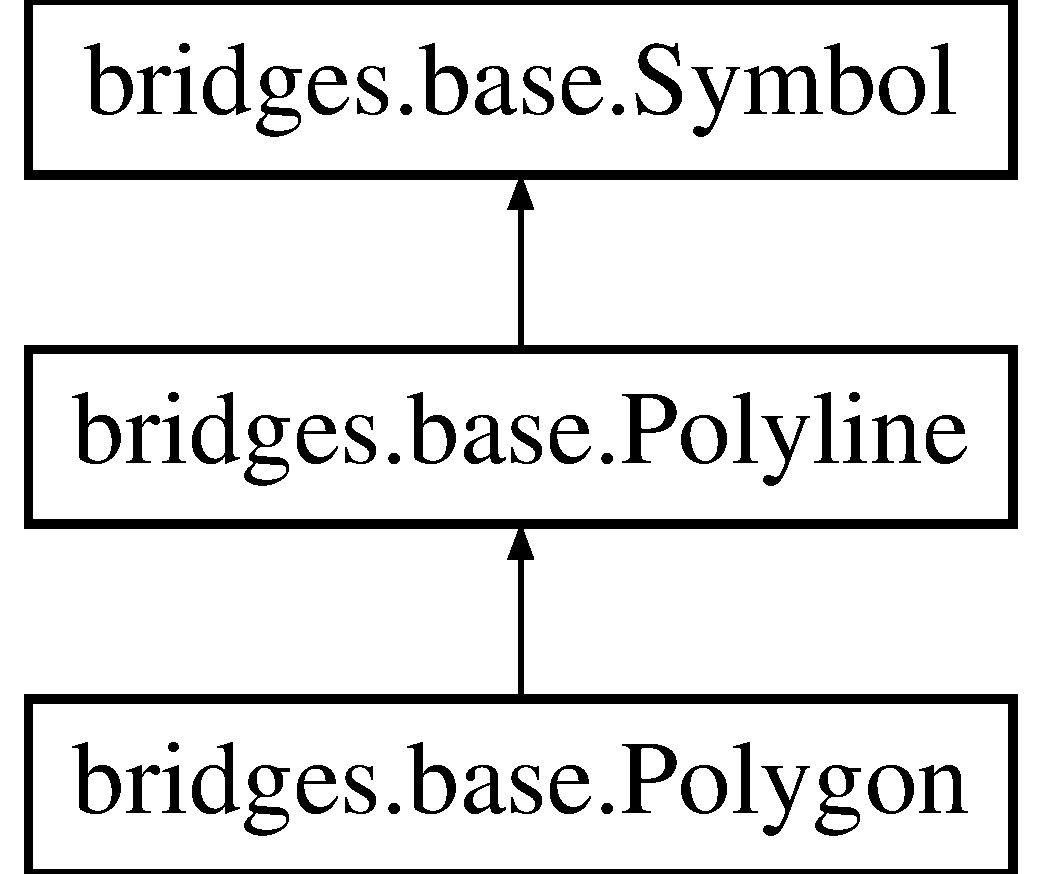
\includegraphics[height=3.000000cm]{classbridges_1_1base_1_1_polygon}
\end{center}
\end{figure}


\subsection{Detailed Description}
This class defines a polygon and is part of the symbol collection. A polygon has a sequence of 2D points (x, y coordinate pairs) 

Basic styling such as stroke, fill, color are defined in the superclass \hyperlink{classbridges_1_1base_1_1_symbol}{Symbol}.

\begin{DoxySeeAlso}{See also}
An example tutorial can be found at \href{http://bridgesuncc.github.io/tutorials/Symbol_Collection.html}{\tt http\+://bridgesuncc.\+github.\+io/tutorials/\+Symbol\+\_\+\+Collection.\+html}
\end{DoxySeeAlso}
\begin{DoxyAuthor}{Author}
David Burlinson, Kalpathi Subramanian 
\end{DoxyAuthor}
\begin{DoxyDate}{Date}
12/23/18, 7/15/19 
\end{DoxyDate}
\subsection*{Public Member Functions}
\begin{DoxyCompactItemize}
\item 
\hyperlink{classbridges_1_1base_1_1_polygon_af0c1b3bc3147ffbda98fd9c515a8052d}{Polygon} ()
\item 
\hyperlink{classbridges_1_1base_1_1_polygon_a341cc297ba7f0f201d31aa3c98ecf108}{Polygon} (Array\+List$<$ Float $>$ pts)
\item 
String \hyperlink{classbridges_1_1base_1_1_polygon_a2203367acb1a26dfa1a81d69ce61274f}{get\+Name} ()
\end{DoxyCompactItemize}
\subsection*{Additional Inherited Members}


\subsection{Constructor \& Destructor Documentation}
\mbox{\Hypertarget{classbridges_1_1base_1_1_polygon_af0c1b3bc3147ffbda98fd9c515a8052d}\label{classbridges_1_1base_1_1_polygon_af0c1b3bc3147ffbda98fd9c515a8052d}} 
\index{bridges\+::base\+::\+Polygon@{bridges\+::base\+::\+Polygon}!Polygon@{Polygon}}
\index{Polygon@{Polygon}!bridges\+::base\+::\+Polygon@{bridges\+::base\+::\+Polygon}}
\subsubsection{\texorpdfstring{Polygon()}{Polygon()}\hspace{0.1cm}{\footnotesize\ttfamily [1/2]}}
{\footnotesize\ttfamily bridges.\+base.\+Polygon.\+Polygon (\begin{DoxyParamCaption}{ }\end{DoxyParamCaption})}

Construct a default polygon structure \mbox{\Hypertarget{classbridges_1_1base_1_1_polygon_a341cc297ba7f0f201d31aa3c98ecf108}\label{classbridges_1_1base_1_1_polygon_a341cc297ba7f0f201d31aa3c98ecf108}} 
\index{bridges\+::base\+::\+Polygon@{bridges\+::base\+::\+Polygon}!Polygon@{Polygon}}
\index{Polygon@{Polygon}!bridges\+::base\+::\+Polygon@{bridges\+::base\+::\+Polygon}}
\subsubsection{\texorpdfstring{Polygon()}{Polygon()}\hspace{0.1cm}{\footnotesize\ttfamily [2/2]}}
{\footnotesize\ttfamily bridges.\+base.\+Polygon.\+Polygon (\begin{DoxyParamCaption}\item[{Array\+List$<$ Float $>$}]{pts }\end{DoxyParamCaption})}

Construct a polygon with the give set of points 
\begin{DoxyParams}{Parameters}
{\em pts} & the array of 2D points \\
\hline
\end{DoxyParams}


\subsection{Member Function Documentation}
\mbox{\Hypertarget{classbridges_1_1base_1_1_polygon_a2203367acb1a26dfa1a81d69ce61274f}\label{classbridges_1_1base_1_1_polygon_a2203367acb1a26dfa1a81d69ce61274f}} 
\index{bridges\+::base\+::\+Polygon@{bridges\+::base\+::\+Polygon}!get\+Name@{get\+Name}}
\index{get\+Name@{get\+Name}!bridges\+::base\+::\+Polygon@{bridges\+::base\+::\+Polygon}}
\subsubsection{\texorpdfstring{get\+Name()}{getName()}}
{\footnotesize\ttfamily String bridges.\+base.\+Polygon.\+get\+Name (\begin{DoxyParamCaption}{ }\end{DoxyParamCaption})}

This method gets the name of the shape

\begin{DoxyReturn}{Returns}
name shape name 
\end{DoxyReturn}


The documentation for this class was generated from the following file\+:\begin{DoxyCompactItemize}
\item 
/home/erik/work/bridges/bridges-\/java/src/main/java/bridges/base/\hyperlink{_polygon_8java}{Polygon.\+java}\end{DoxyCompactItemize}

\hypertarget{classbridges_1_1base_1_1_polyline}{}\doxysection{bridges.\+base.\+Polyline Class Reference}
\label{classbridges_1_1base_1_1_polyline}\index{bridges.base.Polyline@{bridges.base.Polyline}}
Inheritance diagram for bridges.\+base.\+Polyline\+:\begin{figure}[H]
\begin{center}
\leavevmode
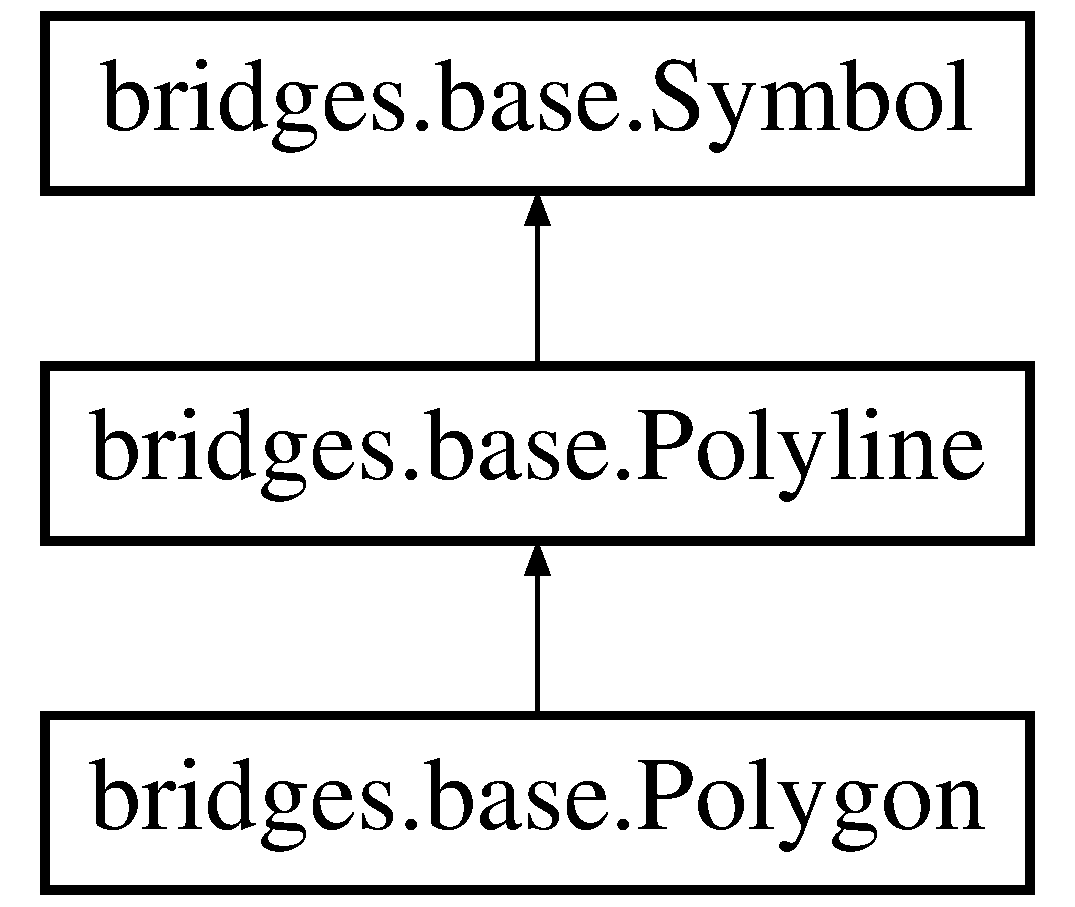
\includegraphics[height=3.000000cm]{classbridges_1_1base_1_1_polyline}
\end{center}
\end{figure}


\doxysubsection{Detailed Description}
This class defines a polyline and is part of the symbol collection. A polyline has a sequence of points (x, y coordinate pairs) 

Basic styling such as stroke and fill are defined in the superclass \mbox{\hyperlink{classbridges_1_1base_1_1_symbol}{Symbol}}.

\begin{DoxyAuthor}{Author}
David Burlinson, Kalpathi Subramanian 
\end{DoxyAuthor}
\begin{DoxyDate}{Date}
12/23/18, 7/15/19 
\end{DoxyDate}
\doxysubsection*{Public Member Functions}
\begin{DoxyCompactItemize}
\item 
\mbox{\hyperlink{classbridges_1_1base_1_1_polyline_a8842a3d3737dfa5b26424a05dc965a4b}{Polyline}} ()
\item 
\mbox{\hyperlink{classbridges_1_1base_1_1_polyline_a11d14fddddd6e89e0902e94aa1bac875}{Polyline}} (Array\+List$<$ Float $>$ pts)
\item 
String \mbox{\hyperlink{classbridges_1_1base_1_1_polyline_a5b56cee642a6381ea940c75a336076ea}{get\+Name}} ()
\item 
void \mbox{\hyperlink{classbridges_1_1base_1_1_polyline_a24b99307181f1a938ea408355984d191}{add\+Point}} (float x, float y)
\item 
Array\+List$<$ Float $>$ \mbox{\hyperlink{classbridges_1_1base_1_1_polyline_ae610d680975558db90a06949991583f8}{get\+Points}} ()
\item 
void \mbox{\hyperlink{classbridges_1_1base_1_1_polyline_a3fec0c95e9f26b173cba105bd39e9df1}{set\+Polyline}} (Array\+List$<$ Float $>$ pts)
\item 
float \mbox{[}$\,$\mbox{]} \mbox{\hyperlink{classbridges_1_1base_1_1_polyline_a5665bd906b841ca71a668581aeb7a181}{get\+Dimensions}} ()
\item 
J\+S\+O\+N\+Object \mbox{\hyperlink{classbridges_1_1base_1_1_polyline_a4ac266909645f8db9b7fcc4836f6069a}{get\+J\+S\+O\+N\+Representation}} ()
\end{DoxyCompactItemize}
\doxysubsection*{Additional Inherited Members}


\doxysubsection{Constructor \& Destructor Documentation}
\mbox{\Hypertarget{classbridges_1_1base_1_1_polyline_a8842a3d3737dfa5b26424a05dc965a4b}\label{classbridges_1_1base_1_1_polyline_a8842a3d3737dfa5b26424a05dc965a4b}} 
\index{bridges.base.Polyline@{bridges.base.Polyline}!Polyline@{Polyline}}
\index{Polyline@{Polyline}!bridges.base.Polyline@{bridges.base.Polyline}}
\doxysubsubsection{\texorpdfstring{Polyline()}{Polyline()}\hspace{0.1cm}{\footnotesize\ttfamily [1/2]}}
{\footnotesize\ttfamily bridges.\+base.\+Polyline.\+Polyline (\begin{DoxyParamCaption}{ }\end{DoxyParamCaption})}

Construct a default polyline structure \mbox{\Hypertarget{classbridges_1_1base_1_1_polyline_a11d14fddddd6e89e0902e94aa1bac875}\label{classbridges_1_1base_1_1_polyline_a11d14fddddd6e89e0902e94aa1bac875}} 
\index{bridges.base.Polyline@{bridges.base.Polyline}!Polyline@{Polyline}}
\index{Polyline@{Polyline}!bridges.base.Polyline@{bridges.base.Polyline}}
\doxysubsubsection{\texorpdfstring{Polyline()}{Polyline()}\hspace{0.1cm}{\footnotesize\ttfamily [2/2]}}
{\footnotesize\ttfamily bridges.\+base.\+Polyline.\+Polyline (\begin{DoxyParamCaption}\item[{Array\+List$<$ Float $>$}]{pts }\end{DoxyParamCaption})}

Construct a polyline with the give set of points 

\doxysubsection{Member Function Documentation}
\mbox{\Hypertarget{classbridges_1_1base_1_1_polyline_a24b99307181f1a938ea408355984d191}\label{classbridges_1_1base_1_1_polyline_a24b99307181f1a938ea408355984d191}} 
\index{bridges.base.Polyline@{bridges.base.Polyline}!addPoint@{addPoint}}
\index{addPoint@{addPoint}!bridges.base.Polyline@{bridges.base.Polyline}}
\doxysubsubsection{\texorpdfstring{addPoint()}{addPoint()}}
{\footnotesize\ttfamily void bridges.\+base.\+Polyline.\+add\+Point (\begin{DoxyParamCaption}\item[{float}]{x,  }\item[{float}]{y }\end{DoxyParamCaption})}

This method adds a point to the polyline


\begin{DoxyParams}{Parameters}
{\em x,y} & Coordinates of the point \\
\hline
\end{DoxyParams}
\mbox{\Hypertarget{classbridges_1_1base_1_1_polyline_a5665bd906b841ca71a668581aeb7a181}\label{classbridges_1_1base_1_1_polyline_a5665bd906b841ca71a668581aeb7a181}} 
\index{bridges.base.Polyline@{bridges.base.Polyline}!getDimensions@{getDimensions}}
\index{getDimensions@{getDimensions}!bridges.base.Polyline@{bridges.base.Polyline}}
\doxysubsubsection{\texorpdfstring{getDimensions()}{getDimensions()}}
{\footnotesize\ttfamily float \mbox{[}$\,$\mbox{]} bridges.\+base.\+Polyline.\+get\+Dimensions (\begin{DoxyParamCaption}{ }\end{DoxyParamCaption})}

This method returns the dimensions of the shape\+: min and max values in X and Y

\begin{DoxyReturn}{Returns}
Bounding box of the point list (array of 4 values) 
\end{DoxyReturn}


Reimplemented from \mbox{\hyperlink{classbridges_1_1base_1_1_symbol_a6cf741f603dd6347325e95a2b4d13d2e}{bridges.\+base.\+Symbol}}.

\mbox{\Hypertarget{classbridges_1_1base_1_1_polyline_a4ac266909645f8db9b7fcc4836f6069a}\label{classbridges_1_1base_1_1_polyline_a4ac266909645f8db9b7fcc4836f6069a}} 
\index{bridges.base.Polyline@{bridges.base.Polyline}!getJSONRepresentation@{getJSONRepresentation}}
\index{getJSONRepresentation@{getJSONRepresentation}!bridges.base.Polyline@{bridges.base.Polyline}}
\doxysubsubsection{\texorpdfstring{getJSONRepresentation()}{getJSONRepresentation()}}
{\footnotesize\ttfamily J\+S\+O\+N\+Object bridges.\+base.\+Polyline.\+get\+J\+S\+O\+N\+Representation (\begin{DoxyParamCaption}{ }\end{DoxyParamCaption})}

This method returns the J\+S\+ON representation of the shape

\begin{DoxyReturn}{Returns}
string J\+S\+ON string 
\end{DoxyReturn}


Reimplemented from \mbox{\hyperlink{classbridges_1_1base_1_1_symbol_aeba4cfa5b39fe03e72a568a8b7452e60}{bridges.\+base.\+Symbol}}.

\mbox{\Hypertarget{classbridges_1_1base_1_1_polyline_a5b56cee642a6381ea940c75a336076ea}\label{classbridges_1_1base_1_1_polyline_a5b56cee642a6381ea940c75a336076ea}} 
\index{bridges.base.Polyline@{bridges.base.Polyline}!getName@{getName}}
\index{getName@{getName}!bridges.base.Polyline@{bridges.base.Polyline}}
\doxysubsubsection{\texorpdfstring{getName()}{getName()}}
{\footnotesize\ttfamily String bridges.\+base.\+Polyline.\+get\+Name (\begin{DoxyParamCaption}{ }\end{DoxyParamCaption})}

This method gets the name of the shape

\begin{DoxyReturn}{Returns}
shape name 
\end{DoxyReturn}


Reimplemented in \mbox{\hyperlink{classbridges_1_1base_1_1_polygon_a2203367acb1a26dfa1a81d69ce61274f}{bridges.\+base.\+Polygon}}.

\mbox{\Hypertarget{classbridges_1_1base_1_1_polyline_ae610d680975558db90a06949991583f8}\label{classbridges_1_1base_1_1_polyline_ae610d680975558db90a06949991583f8}} 
\index{bridges.base.Polyline@{bridges.base.Polyline}!getPoints@{getPoints}}
\index{getPoints@{getPoints}!bridges.base.Polyline@{bridges.base.Polyline}}
\doxysubsubsection{\texorpdfstring{getPoints()}{getPoints()}}
{\footnotesize\ttfamily Array\+List$<$Float$>$ bridges.\+base.\+Polyline.\+get\+Points (\begin{DoxyParamCaption}{ }\end{DoxyParamCaption})}

This method returns the point list of the polyline

\begin{DoxyReturn}{Returns}
points point list of the polyline -\/ sequence of x, y values 
\end{DoxyReturn}
\mbox{\Hypertarget{classbridges_1_1base_1_1_polyline_a3fec0c95e9f26b173cba105bd39e9df1}\label{classbridges_1_1base_1_1_polyline_a3fec0c95e9f26b173cba105bd39e9df1}} 
\index{bridges.base.Polyline@{bridges.base.Polyline}!setPolyline@{setPolyline}}
\index{setPolyline@{setPolyline}!bridges.base.Polyline@{bridges.base.Polyline}}
\doxysubsubsection{\texorpdfstring{setPolyline()}{setPolyline()}}
{\footnotesize\ttfamily void bridges.\+base.\+Polyline.\+set\+Polyline (\begin{DoxyParamCaption}\item[{Array\+List$<$ Float $>$}]{pts }\end{DoxyParamCaption})}



The documentation for this class was generated from the following file\+:\begin{DoxyCompactItemize}
\item 
/\+Users/kalpathi/gr/bridges/client/java/src/main/java/bridges/base/\mbox{\hyperlink{_polyline_8java}{Polyline.\+java}}\end{DoxyCompactItemize}

\hypertarget{classbridges_1_1validation_1_1_rate_limit_exception}{}\doxysection{bridges.\+validation.\+Rate\+Limit\+Exception Class Reference}
\label{classbridges_1_1validation_1_1_rate_limit_exception}\index{bridges.validation.RateLimitException@{bridges.validation.RateLimitException}}
Inheritance diagram for bridges.\+validation.\+Rate\+Limit\+Exception\+:\begin{figure}[H]
\begin{center}
\leavevmode
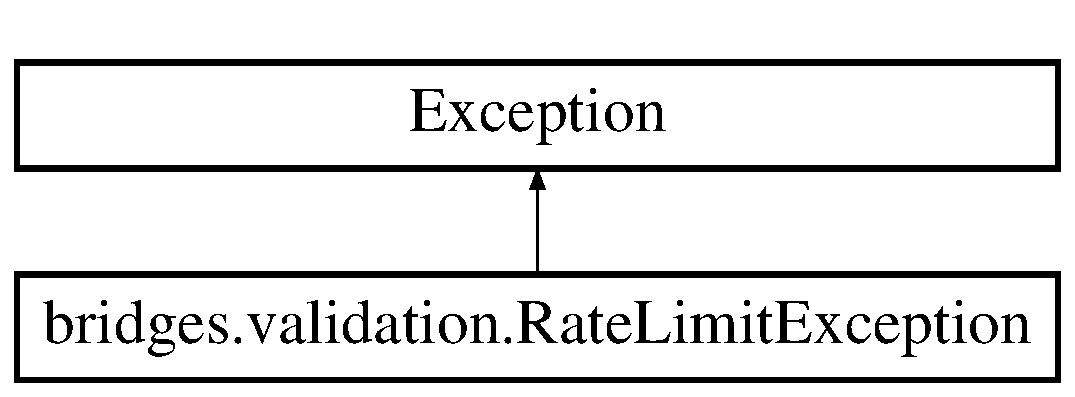
\includegraphics[height=2.000000cm]{classbridges_1_1validation_1_1_rate_limit_exception}
\end{center}
\end{figure}
\doxysubsection*{Public Member Functions}
\begin{DoxyCompactItemize}
\item 
\mbox{\hyperlink{classbridges_1_1validation_1_1_rate_limit_exception_a8375495a80a80213fe9201921c43afbc}{Rate\+Limit\+Exception}} (String string)
\end{DoxyCompactItemize}


\doxysubsection{Detailed Description}
Throws exception to handle overloading the server to allow the student to stop querying the server and send in their visualizations. This exception is expected every time the program runs to limit the amount of requests going to Twitter etc.

\begin{DoxyAuthor}{Author}
Michael 
\end{DoxyAuthor}


\doxysubsection{Constructor \& Destructor Documentation}
\mbox{\Hypertarget{classbridges_1_1validation_1_1_rate_limit_exception_a8375495a80a80213fe9201921c43afbc}\label{classbridges_1_1validation_1_1_rate_limit_exception_a8375495a80a80213fe9201921c43afbc}} 
\index{bridges.validation.RateLimitException@{bridges.validation.RateLimitException}!RateLimitException@{RateLimitException}}
\index{RateLimitException@{RateLimitException}!bridges.validation.RateLimitException@{bridges.validation.RateLimitException}}
\doxysubsubsection{\texorpdfstring{RateLimitException()}{RateLimitException()}}
{\footnotesize\ttfamily bridges.\+validation.\+Rate\+Limit\+Exception.\+Rate\+Limit\+Exception (\begin{DoxyParamCaption}\item[{String}]{string }\end{DoxyParamCaption})}



The documentation for this class was generated from the following file\+:\begin{DoxyCompactItemize}
\item 
/\+Users/kalpathi/gr/bridges/client/java/src/main/java/bridges/validation/\mbox{\hyperlink{_rate_limit_exception_8java}{Rate\+Limit\+Exception.\+java}}\end{DoxyCompactItemize}

\hypertarget{classbridges_1_1base_1_1_rectangle}{}\section{bridges.\+base.\+Rectangle Class Reference}
\label{classbridges_1_1base_1_1_rectangle}\index{bridges.\+base.\+Rectangle@{bridges.\+base.\+Rectangle}}


This class defines a rectangle and is part of the symbol collection. A rectangle has height and width.  


Inheritance diagram for bridges.\+base.\+Rectangle\+:\begin{figure}[H]
\begin{center}
\leavevmode
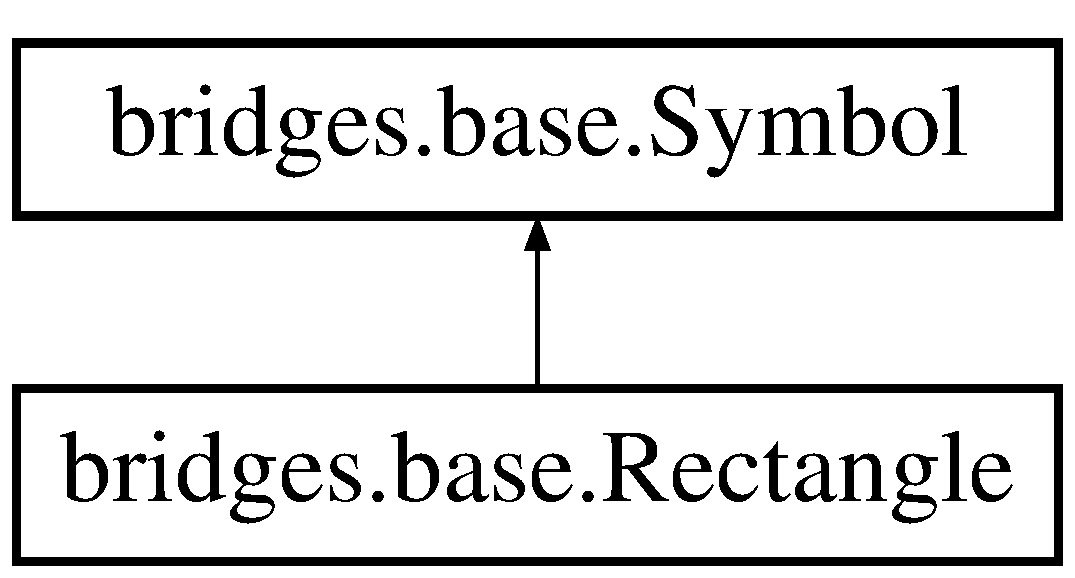
\includegraphics[height=3.000000cm]{classbridges_1_1base_1_1_rectangle}
\end{center}
\end{figure}
\subsection*{Public Member Functions}
\begin{DoxyCompactItemize}
\item 
\mbox{\hyperlink{classbridges_1_1base_1_1_rectangle_a6d80c63a14e9b94df552dac422348dc3}{Rectangle}} ()
\item 
\mbox{\hyperlink{classbridges_1_1base_1_1_rectangle_a8e7e936bf76b597c097a9786cf02cf77}{Rectangle}} (int w, int h)
\item 
\mbox{\hyperlink{classbridges_1_1base_1_1_rectangle_ade3310629f09ee38c57853108d387628}{Rectangle}} (Float locx, Float locy, int w, int h)
\item 
String \mbox{\hyperlink{classbridges_1_1base_1_1_rectangle_ab785b45f264ae3cd61a5a898ffa6afba}{get\+Name}} ()
\item 
void \mbox{\hyperlink{classbridges_1_1base_1_1_rectangle_a803ca26bb6bb0c29c9316d910fce0fe1}{set\+Width}} (int w)
\item 
Float \mbox{[}$\,$\mbox{]} \mbox{\hyperlink{classbridges_1_1base_1_1_rectangle_a9a903d4617cde354f617ac4e8625fa38}{get\+Dimensions}} ()
\item 
void \mbox{\hyperlink{classbridges_1_1base_1_1_rectangle_a7f071805534af749355f3d6122972ab9}{set\+Rectangle}} (Float locx, Float locy, int w, int h)
\item 
J\+S\+O\+N\+Object \mbox{\hyperlink{classbridges_1_1base_1_1_rectangle_ad9a44cbdc301594b8708769461ad4461}{get\+J\+S\+O\+N\+Representation}} ()
\end{DoxyCompactItemize}
\subsection*{Additional Inherited Members}


\subsection{Detailed Description}
This class defines a rectangle and is part of the symbol collection. A rectangle has height and width. 

\begin{DoxyAuthor}{Author}
Kalpathi Subramanian 
\end{DoxyAuthor}
\begin{DoxyDate}{Date}
12/23/18 
\end{DoxyDate}


\subsection{Constructor \& Destructor Documentation}
\mbox{\Hypertarget{classbridges_1_1base_1_1_rectangle_a6d80c63a14e9b94df552dac422348dc3}\label{classbridges_1_1base_1_1_rectangle_a6d80c63a14e9b94df552dac422348dc3}} 
\index{bridges\+::base\+::\+Rectangle@{bridges\+::base\+::\+Rectangle}!Rectangle@{Rectangle}}
\index{Rectangle@{Rectangle}!bridges\+::base\+::\+Rectangle@{bridges\+::base\+::\+Rectangle}}
\subsubsection{\texorpdfstring{Rectangle()}{Rectangle()}\hspace{0.1cm}{\footnotesize\ttfamily [1/3]}}
{\footnotesize\ttfamily bridges.\+base.\+Rectangle.\+Rectangle (\begin{DoxyParamCaption}{ }\end{DoxyParamCaption})}

constructors \mbox{\Hypertarget{classbridges_1_1base_1_1_rectangle_a8e7e936bf76b597c097a9786cf02cf77}\label{classbridges_1_1base_1_1_rectangle_a8e7e936bf76b597c097a9786cf02cf77}} 
\index{bridges\+::base\+::\+Rectangle@{bridges\+::base\+::\+Rectangle}!Rectangle@{Rectangle}}
\index{Rectangle@{Rectangle}!bridges\+::base\+::\+Rectangle@{bridges\+::base\+::\+Rectangle}}
\subsubsection{\texorpdfstring{Rectangle()}{Rectangle()}\hspace{0.1cm}{\footnotesize\ttfamily [2/3]}}
{\footnotesize\ttfamily bridges.\+base.\+Rectangle.\+Rectangle (\begin{DoxyParamCaption}\item[{int}]{w,  }\item[{int}]{h }\end{DoxyParamCaption})}

\mbox{\Hypertarget{classbridges_1_1base_1_1_rectangle_ade3310629f09ee38c57853108d387628}\label{classbridges_1_1base_1_1_rectangle_ade3310629f09ee38c57853108d387628}} 
\index{bridges\+::base\+::\+Rectangle@{bridges\+::base\+::\+Rectangle}!Rectangle@{Rectangle}}
\index{Rectangle@{Rectangle}!bridges\+::base\+::\+Rectangle@{bridges\+::base\+::\+Rectangle}}
\subsubsection{\texorpdfstring{Rectangle()}{Rectangle()}\hspace{0.1cm}{\footnotesize\ttfamily [3/3]}}
{\footnotesize\ttfamily bridges.\+base.\+Rectangle.\+Rectangle (\begin{DoxyParamCaption}\item[{Float}]{locx,  }\item[{Float}]{locy,  }\item[{int}]{w,  }\item[{int}]{h }\end{DoxyParamCaption})}



\subsection{Member Function Documentation}
\mbox{\Hypertarget{classbridges_1_1base_1_1_rectangle_a9a903d4617cde354f617ac4e8625fa38}\label{classbridges_1_1base_1_1_rectangle_a9a903d4617cde354f617ac4e8625fa38}} 
\index{bridges\+::base\+::\+Rectangle@{bridges\+::base\+::\+Rectangle}!get\+Dimensions@{get\+Dimensions}}
\index{get\+Dimensions@{get\+Dimensions}!bridges\+::base\+::\+Rectangle@{bridges\+::base\+::\+Rectangle}}
\subsubsection{\texorpdfstring{get\+Dimensions()}{getDimensions()}}
{\footnotesize\ttfamily Float \mbox{[}$\,$\mbox{]} bridges.\+base.\+Rectangle.\+get\+Dimensions (\begin{DoxyParamCaption}{ }\end{DoxyParamCaption})}

This method returns the dimensions of the shape\+: min and max values in X and Y


\begin{DoxyParams}{Parameters}
{\em none} & \\
\hline
\end{DoxyParams}
\begin{DoxyReturn}{Returns}
array of 4 values 
\end{DoxyReturn}
\mbox{\Hypertarget{classbridges_1_1base_1_1_rectangle_ad9a44cbdc301594b8708769461ad4461}\label{classbridges_1_1base_1_1_rectangle_ad9a44cbdc301594b8708769461ad4461}} 
\index{bridges\+::base\+::\+Rectangle@{bridges\+::base\+::\+Rectangle}!get\+J\+S\+O\+N\+Representation@{get\+J\+S\+O\+N\+Representation}}
\index{get\+J\+S\+O\+N\+Representation@{get\+J\+S\+O\+N\+Representation}!bridges\+::base\+::\+Rectangle@{bridges\+::base\+::\+Rectangle}}
\subsubsection{\texorpdfstring{get\+J\+S\+O\+N\+Representation()}{getJSONRepresentation()}}
{\footnotesize\ttfamily J\+S\+O\+N\+Object bridges.\+base.\+Rectangle.\+get\+J\+S\+O\+N\+Representation (\begin{DoxyParamCaption}{ }\end{DoxyParamCaption})}

This method returns the J\+S\+ON representation of the shape

\begin{DoxyReturn}{Returns}
String J\+S\+ON string 
\end{DoxyReturn}
\mbox{\Hypertarget{classbridges_1_1base_1_1_rectangle_ab785b45f264ae3cd61a5a898ffa6afba}\label{classbridges_1_1base_1_1_rectangle_ab785b45f264ae3cd61a5a898ffa6afba}} 
\index{bridges\+::base\+::\+Rectangle@{bridges\+::base\+::\+Rectangle}!get\+Name@{get\+Name}}
\index{get\+Name@{get\+Name}!bridges\+::base\+::\+Rectangle@{bridges\+::base\+::\+Rectangle}}
\subsubsection{\texorpdfstring{get\+Name()}{getName()}}
{\footnotesize\ttfamily String bridges.\+base.\+Rectangle.\+get\+Name (\begin{DoxyParamCaption}{ }\end{DoxyParamCaption})}

This method gets the name of the shape

\begin{DoxyReturn}{Returns}
name shape name 
\end{DoxyReturn}
\mbox{\Hypertarget{classbridges_1_1base_1_1_rectangle_a7f071805534af749355f3d6122972ab9}\label{classbridges_1_1base_1_1_rectangle_a7f071805534af749355f3d6122972ab9}} 
\index{bridges\+::base\+::\+Rectangle@{bridges\+::base\+::\+Rectangle}!set\+Rectangle@{set\+Rectangle}}
\index{set\+Rectangle@{set\+Rectangle}!bridges\+::base\+::\+Rectangle@{bridges\+::base\+::\+Rectangle}}
\subsubsection{\texorpdfstring{set\+Rectangle()}{setRectangle()}}
{\footnotesize\ttfamily void bridges.\+base.\+Rectangle.\+set\+Rectangle (\begin{DoxyParamCaption}\item[{Float}]{locx,  }\item[{Float}]{locy,  }\item[{int}]{w,  }\item[{int}]{h }\end{DoxyParamCaption})}

\mbox{\Hypertarget{classbridges_1_1base_1_1_rectangle_a803ca26bb6bb0c29c9316d910fce0fe1}\label{classbridges_1_1base_1_1_rectangle_a803ca26bb6bb0c29c9316d910fce0fe1}} 
\index{bridges\+::base\+::\+Rectangle@{bridges\+::base\+::\+Rectangle}!set\+Width@{set\+Width}}
\index{set\+Width@{set\+Width}!bridges\+::base\+::\+Rectangle@{bridges\+::base\+::\+Rectangle}}
\subsubsection{\texorpdfstring{set\+Width()}{setWidth()}}
{\footnotesize\ttfamily void bridges.\+base.\+Rectangle.\+set\+Width (\begin{DoxyParamCaption}\item[{int}]{w }\end{DoxyParamCaption})}

This method sets the shape width


\begin{DoxyParams}{Parameters}
{\em w} & width \\
\hline
\end{DoxyParams}


The documentation for this class was generated from the following file\+:\begin{DoxyCompactItemize}
\item 
/\+Users/kalpathi/gr/bridges/client/java/bridges-\/17/src/main/java/bridges/base/\mbox{\hyperlink{_rectangle_8java}{Rectangle.\+java}}\end{DoxyCompactItemize}

\hypertarget{classbridges_1_1data__src__dependent_1_1_shakespeare}{}\section{bridges.\+data\+\_\+src\+\_\+dependent.\+Shakespeare Class Reference}
\label{classbridges_1_1data__src__dependent_1_1_shakespeare}\index{bridges.\+data\+\_\+src\+\_\+dependent.\+Shakespeare@{bridges.\+data\+\_\+src\+\_\+dependent.\+Shakespeare}}


A \mbox{\hyperlink{classbridges_1_1data__src__dependent_1_1_shakespeare}{Shakespeare}} Data source object containing sonnets, poems and plays.  




Inherits bridges.\+data\+\_\+src\+\_\+dependent.\+Data\+Source.

\subsection*{Public Member Functions}
\begin{DoxyCompactItemize}
\item 
\mbox{\hyperlink{classbridges_1_1data__src__dependent_1_1_shakespeare_a34d92b817c4073000de003362e3003fa}{Shakespeare}} ()
\item 
\mbox{\hyperlink{classbridges_1_1data__src__dependent_1_1_shakespeare_aa5a5390d6f7afe3d63f4ad7f9779f9e9}{Shakespeare}} (String title, String type, String text)
\item 
String \mbox{\hyperlink{classbridges_1_1data__src__dependent_1_1_shakespeare_a0f045c5d1140414b7ad6ad5511e6e79c}{get\+Title}} ()
\item 
void \mbox{\hyperlink{classbridges_1_1data__src__dependent_1_1_shakespeare_a2687017aca35bb26b148f784a0bff732}{set\+Title}} (String title)
\item 
String \mbox{\hyperlink{classbridges_1_1data__src__dependent_1_1_shakespeare_adbbb48b9e2564ae910e0313dd88542fd}{get\+Type}} ()
\item 
void \mbox{\hyperlink{classbridges_1_1data__src__dependent_1_1_shakespeare_afcee18014d5630a0a15701635005bea2}{set\+Type}} (String type)
\item 
String \mbox{\hyperlink{classbridges_1_1data__src__dependent_1_1_shakespeare_a5a5cffa6bf3d35182ba1eed2be19d74d}{get\+Text}} ()
\item 
void \mbox{\hyperlink{classbridges_1_1data__src__dependent_1_1_shakespeare_aa2ae0bee864990ae11950039636e52b1}{set\+Text}} (String text)
\end{DoxyCompactItemize}


\subsection{Detailed Description}
A \mbox{\hyperlink{classbridges_1_1data__src__dependent_1_1_shakespeare}{Shakespeare}} Data source object containing sonnets, poems and plays. 

This is a convenience class provided for users who wish to use this data source as part of their application. It provides an A\+PI that makes it easy to access the attributes of this data set.

Refer to tutorial examples to using this data source in data structure assignments.

Refer to tutorial examples to using this data source in data structure assignments.

\begin{DoxyAuthor}{Author}
Kalpathi Subramanian 
\end{DoxyAuthor}
\begin{DoxyDate}{Date}
2/1/17 
\end{DoxyDate}


\subsection{Constructor \& Destructor Documentation}
\mbox{\Hypertarget{classbridges_1_1data__src__dependent_1_1_shakespeare_a34d92b817c4073000de003362e3003fa}\label{classbridges_1_1data__src__dependent_1_1_shakespeare_a34d92b817c4073000de003362e3003fa}} 
\index{bridges\+::data\+\_\+src\+\_\+dependent\+::\+Shakespeare@{bridges\+::data\+\_\+src\+\_\+dependent\+::\+Shakespeare}!Shakespeare@{Shakespeare}}
\index{Shakespeare@{Shakespeare}!bridges\+::data\+\_\+src\+\_\+dependent\+::\+Shakespeare@{bridges\+::data\+\_\+src\+\_\+dependent\+::\+Shakespeare}}
\subsubsection{\texorpdfstring{Shakespeare()}{Shakespeare()}\hspace{0.1cm}{\footnotesize\ttfamily [1/2]}}
{\footnotesize\ttfamily bridges.\+data\+\_\+src\+\_\+dependent.\+Shakespeare.\+Shakespeare (\begin{DoxyParamCaption}{ }\end{DoxyParamCaption})}

\mbox{\Hypertarget{classbridges_1_1data__src__dependent_1_1_shakespeare_aa5a5390d6f7afe3d63f4ad7f9779f9e9}\label{classbridges_1_1data__src__dependent_1_1_shakespeare_aa5a5390d6f7afe3d63f4ad7f9779f9e9}} 
\index{bridges\+::data\+\_\+src\+\_\+dependent\+::\+Shakespeare@{bridges\+::data\+\_\+src\+\_\+dependent\+::\+Shakespeare}!Shakespeare@{Shakespeare}}
\index{Shakespeare@{Shakespeare}!bridges\+::data\+\_\+src\+\_\+dependent\+::\+Shakespeare@{bridges\+::data\+\_\+src\+\_\+dependent\+::\+Shakespeare}}
\subsubsection{\texorpdfstring{Shakespeare()}{Shakespeare()}\hspace{0.1cm}{\footnotesize\ttfamily [2/2]}}
{\footnotesize\ttfamily bridges.\+data\+\_\+src\+\_\+dependent.\+Shakespeare.\+Shakespeare (\begin{DoxyParamCaption}\item[{String}]{title,  }\item[{String}]{type,  }\item[{String}]{text }\end{DoxyParamCaption})}



\subsection{Member Function Documentation}
\mbox{\Hypertarget{classbridges_1_1data__src__dependent_1_1_shakespeare_a5a5cffa6bf3d35182ba1eed2be19d74d}\label{classbridges_1_1data__src__dependent_1_1_shakespeare_a5a5cffa6bf3d35182ba1eed2be19d74d}} 
\index{bridges\+::data\+\_\+src\+\_\+dependent\+::\+Shakespeare@{bridges\+::data\+\_\+src\+\_\+dependent\+::\+Shakespeare}!get\+Text@{get\+Text}}
\index{get\+Text@{get\+Text}!bridges\+::data\+\_\+src\+\_\+dependent\+::\+Shakespeare@{bridges\+::data\+\_\+src\+\_\+dependent\+::\+Shakespeare}}
\subsubsection{\texorpdfstring{get\+Text()}{getText()}}
{\footnotesize\ttfamily String bridges.\+data\+\_\+src\+\_\+dependent.\+Shakespeare.\+get\+Text (\begin{DoxyParamCaption}{ }\end{DoxyParamCaption})}

\mbox{\Hypertarget{classbridges_1_1data__src__dependent_1_1_shakespeare_a0f045c5d1140414b7ad6ad5511e6e79c}\label{classbridges_1_1data__src__dependent_1_1_shakespeare_a0f045c5d1140414b7ad6ad5511e6e79c}} 
\index{bridges\+::data\+\_\+src\+\_\+dependent\+::\+Shakespeare@{bridges\+::data\+\_\+src\+\_\+dependent\+::\+Shakespeare}!get\+Title@{get\+Title}}
\index{get\+Title@{get\+Title}!bridges\+::data\+\_\+src\+\_\+dependent\+::\+Shakespeare@{bridges\+::data\+\_\+src\+\_\+dependent\+::\+Shakespeare}}
\subsubsection{\texorpdfstring{get\+Title()}{getTitle()}}
{\footnotesize\ttfamily String bridges.\+data\+\_\+src\+\_\+dependent.\+Shakespeare.\+get\+Title (\begin{DoxyParamCaption}{ }\end{DoxyParamCaption})}

\mbox{\Hypertarget{classbridges_1_1data__src__dependent_1_1_shakespeare_adbbb48b9e2564ae910e0313dd88542fd}\label{classbridges_1_1data__src__dependent_1_1_shakespeare_adbbb48b9e2564ae910e0313dd88542fd}} 
\index{bridges\+::data\+\_\+src\+\_\+dependent\+::\+Shakespeare@{bridges\+::data\+\_\+src\+\_\+dependent\+::\+Shakespeare}!get\+Type@{get\+Type}}
\index{get\+Type@{get\+Type}!bridges\+::data\+\_\+src\+\_\+dependent\+::\+Shakespeare@{bridges\+::data\+\_\+src\+\_\+dependent\+::\+Shakespeare}}
\subsubsection{\texorpdfstring{get\+Type()}{getType()}}
{\footnotesize\ttfamily String bridges.\+data\+\_\+src\+\_\+dependent.\+Shakespeare.\+get\+Type (\begin{DoxyParamCaption}{ }\end{DoxyParamCaption})}

\mbox{\Hypertarget{classbridges_1_1data__src__dependent_1_1_shakespeare_aa2ae0bee864990ae11950039636e52b1}\label{classbridges_1_1data__src__dependent_1_1_shakespeare_aa2ae0bee864990ae11950039636e52b1}} 
\index{bridges\+::data\+\_\+src\+\_\+dependent\+::\+Shakespeare@{bridges\+::data\+\_\+src\+\_\+dependent\+::\+Shakespeare}!set\+Text@{set\+Text}}
\index{set\+Text@{set\+Text}!bridges\+::data\+\_\+src\+\_\+dependent\+::\+Shakespeare@{bridges\+::data\+\_\+src\+\_\+dependent\+::\+Shakespeare}}
\subsubsection{\texorpdfstring{set\+Text()}{setText()}}
{\footnotesize\ttfamily void bridges.\+data\+\_\+src\+\_\+dependent.\+Shakespeare.\+set\+Text (\begin{DoxyParamCaption}\item[{String}]{text }\end{DoxyParamCaption})}

\mbox{\Hypertarget{classbridges_1_1data__src__dependent_1_1_shakespeare_a2687017aca35bb26b148f784a0bff732}\label{classbridges_1_1data__src__dependent_1_1_shakespeare_a2687017aca35bb26b148f784a0bff732}} 
\index{bridges\+::data\+\_\+src\+\_\+dependent\+::\+Shakespeare@{bridges\+::data\+\_\+src\+\_\+dependent\+::\+Shakespeare}!set\+Title@{set\+Title}}
\index{set\+Title@{set\+Title}!bridges\+::data\+\_\+src\+\_\+dependent\+::\+Shakespeare@{bridges\+::data\+\_\+src\+\_\+dependent\+::\+Shakespeare}}
\subsubsection{\texorpdfstring{set\+Title()}{setTitle()}}
{\footnotesize\ttfamily void bridges.\+data\+\_\+src\+\_\+dependent.\+Shakespeare.\+set\+Title (\begin{DoxyParamCaption}\item[{String}]{title }\end{DoxyParamCaption})}

\mbox{\Hypertarget{classbridges_1_1data__src__dependent_1_1_shakespeare_afcee18014d5630a0a15701635005bea2}\label{classbridges_1_1data__src__dependent_1_1_shakespeare_afcee18014d5630a0a15701635005bea2}} 
\index{bridges\+::data\+\_\+src\+\_\+dependent\+::\+Shakespeare@{bridges\+::data\+\_\+src\+\_\+dependent\+::\+Shakespeare}!set\+Type@{set\+Type}}
\index{set\+Type@{set\+Type}!bridges\+::data\+\_\+src\+\_\+dependent\+::\+Shakespeare@{bridges\+::data\+\_\+src\+\_\+dependent\+::\+Shakespeare}}
\subsubsection{\texorpdfstring{set\+Type()}{setType()}}
{\footnotesize\ttfamily void bridges.\+data\+\_\+src\+\_\+dependent.\+Shakespeare.\+set\+Type (\begin{DoxyParamCaption}\item[{String}]{type }\end{DoxyParamCaption})}



The documentation for this class was generated from the following file\+:\begin{DoxyCompactItemize}
\item 
/\+Users/kalpathi/gr/bridges/client/java/bridges-\/17/src/main/java/edu/uncc/cs/bridges\+\_\+v21/data\+\_\+src\+\_\+dependent/\mbox{\hyperlink{_shakespeare_8java}{Shakespeare.\+java}}\end{DoxyCompactItemize}

\hypertarget{classbridges_1_1benchmark_1_1_shortest_path_benchmark}{}\section{bridges.\+benchmark.\+Shortest\+Path\+Benchmark Class Reference}
\label{classbridges_1_1benchmark_1_1_shortest_path_benchmark}\index{bridges.\+benchmark.\+Shortest\+Path\+Benchmark@{bridges.\+benchmark.\+Shortest\+Path\+Benchmark}}


Inherits bridges.\+benchmark.\+Graph\+Benchmark.



\subsection{Detailed Description}
Benchmarks Shortest Path algorithms. 

Benchmarks Shortest Path algorithms and add time series to a Line\+Chart.

One can also set a maximum time spent on a particular run using set\+Time\+Cap();

and can be passed to the run function for being benchmarked. A typical use would look something like


\begin{DoxyCode}
LineChart lc;
\mbox{\hyperlink{classbridges_1_1benchmark_1_1_shortest_path_benchmark_ad878c2ad9c6912170601092423c54c43}{ShortestPathBenchmark}} sb = \textcolor{keyword}{new} \mbox{\hyperlink{classbridges_1_1benchmark_1_1_shortest_path_benchmark_ad878c2ad9c6912170601092423c54c43}{ShortestPathBenchmark}}(lc);
sb.run(\textcolor{stringliteral}{"mybfsalgorithm"}, spalgo);
\end{DoxyCode}


\begin{DoxyAuthor}{Author}
Erik Saule 
\end{DoxyAuthor}
\begin{DoxyDate}{Date}
07/21/2019 
\end{DoxyDate}
\subsection*{Public Member Functions}
\begin{DoxyCompactItemize}
\item 
\mbox{\hyperlink{classbridges_1_1benchmark_1_1_shortest_path_benchmark_ad878c2ad9c6912170601092423c54c43}{Shortest\+Path\+Benchmark}} (\mbox{\hyperlink{classbridges_1_1base_1_1_line_chart}{Line\+Chart}} plot, long time\+Cap)
\item 
\mbox{\hyperlink{classbridges_1_1benchmark_1_1_shortest_path_benchmark_ac84a2afc6e663b9d4edc61b3d4c4701c}{Shortest\+Path\+Benchmark}} (\mbox{\hyperlink{classbridges_1_1base_1_1_line_chart}{Line\+Chart}} plot)
\item 
void \mbox{\hyperlink{classbridges_1_1benchmark_1_1_shortest_path_benchmark_ad7e6918e142cfbdaac08493ccbf02acf}{run}} (String algo\+Name, Consumer$<$ \mbox{\hyperlink{classbridges_1_1benchmark_1_1_shortest_path_params}{Shortest\+Path\+Params}} $>$ sp\+Algo)  throws I\+O\+Exception 
\begin{DoxyCompactList}\small\item\em benchmark a particular Shortest Path algorithm that accepts a single \mbox{\hyperlink{classbridges_1_1benchmark_1_1_shortest_path_params}{Shortest\+Path\+Params}} argument \end{DoxyCompactList}\end{DoxyCompactItemize}


\subsection{Constructor \& Destructor Documentation}
\mbox{\Hypertarget{classbridges_1_1benchmark_1_1_shortest_path_benchmark_ad878c2ad9c6912170601092423c54c43}\label{classbridges_1_1benchmark_1_1_shortest_path_benchmark_ad878c2ad9c6912170601092423c54c43}} 
\index{bridges\+::benchmark\+::\+Shortest\+Path\+Benchmark@{bridges\+::benchmark\+::\+Shortest\+Path\+Benchmark}!Shortest\+Path\+Benchmark@{Shortest\+Path\+Benchmark}}
\index{Shortest\+Path\+Benchmark@{Shortest\+Path\+Benchmark}!bridges\+::benchmark\+::\+Shortest\+Path\+Benchmark@{bridges\+::benchmark\+::\+Shortest\+Path\+Benchmark}}
\subsubsection{\texorpdfstring{Shortest\+Path\+Benchmark()}{ShortestPathBenchmark()}\hspace{0.1cm}{\footnotesize\ttfamily [1/2]}}
{\footnotesize\ttfamily bridges.\+benchmark.\+Shortest\+Path\+Benchmark.\+Shortest\+Path\+Benchmark (\begin{DoxyParamCaption}\item[{\mbox{\hyperlink{classbridges_1_1base_1_1_line_chart}{Line\+Chart}}}]{plot,  }\item[{long}]{time\+Cap }\end{DoxyParamCaption})}

\mbox{\Hypertarget{classbridges_1_1benchmark_1_1_shortest_path_benchmark_ac84a2afc6e663b9d4edc61b3d4c4701c}\label{classbridges_1_1benchmark_1_1_shortest_path_benchmark_ac84a2afc6e663b9d4edc61b3d4c4701c}} 
\index{bridges\+::benchmark\+::\+Shortest\+Path\+Benchmark@{bridges\+::benchmark\+::\+Shortest\+Path\+Benchmark}!Shortest\+Path\+Benchmark@{Shortest\+Path\+Benchmark}}
\index{Shortest\+Path\+Benchmark@{Shortest\+Path\+Benchmark}!bridges\+::benchmark\+::\+Shortest\+Path\+Benchmark@{bridges\+::benchmark\+::\+Shortest\+Path\+Benchmark}}
\subsubsection{\texorpdfstring{Shortest\+Path\+Benchmark()}{ShortestPathBenchmark()}\hspace{0.1cm}{\footnotesize\ttfamily [2/2]}}
{\footnotesize\ttfamily bridges.\+benchmark.\+Shortest\+Path\+Benchmark.\+Shortest\+Path\+Benchmark (\begin{DoxyParamCaption}\item[{\mbox{\hyperlink{classbridges_1_1base_1_1_line_chart}{Line\+Chart}}}]{plot }\end{DoxyParamCaption})}



\subsection{Member Function Documentation}
\mbox{\Hypertarget{classbridges_1_1benchmark_1_1_shortest_path_benchmark_ad7e6918e142cfbdaac08493ccbf02acf}\label{classbridges_1_1benchmark_1_1_shortest_path_benchmark_ad7e6918e142cfbdaac08493ccbf02acf}} 
\index{bridges\+::benchmark\+::\+Shortest\+Path\+Benchmark@{bridges\+::benchmark\+::\+Shortest\+Path\+Benchmark}!run@{run}}
\index{run@{run}!bridges\+::benchmark\+::\+Shortest\+Path\+Benchmark@{bridges\+::benchmark\+::\+Shortest\+Path\+Benchmark}}
\subsubsection{\texorpdfstring{run()}{run()}}
{\footnotesize\ttfamily void bridges.\+benchmark.\+Shortest\+Path\+Benchmark.\+run (\begin{DoxyParamCaption}\item[{String}]{algo\+Name,  }\item[{Consumer$<$ \mbox{\hyperlink{classbridges_1_1benchmark_1_1_shortest_path_params}{Shortest\+Path\+Params}} $>$}]{sp\+Algo }\end{DoxyParamCaption}) throws I\+O\+Exception}



benchmark a particular Shortest Path algorithm that accepts a single \mbox{\hyperlink{classbridges_1_1benchmark_1_1_shortest_path_params}{Shortest\+Path\+Params}} argument 


\begin{DoxyParams}{Parameters}
{\em algo\+Name} & Screen name of the algorithm \\
\hline
{\em sp\+Algo} & the actual algorithm \\
\hline
\end{DoxyParams}


The documentation for this class was generated from the following file\+:\begin{DoxyCompactItemize}
\item 
/\+Users/kalpathi/gr/bridges/client/java/src/main/java/bridges/benchmark/\mbox{\hyperlink{_shortest_path_benchmark_8java}{Shortest\+Path\+Benchmark.\+java}}\end{DoxyCompactItemize}

\hypertarget{classbridges_1_1benchmark_1_1_shortest_path_params}{}\doxysection{bridges.\+benchmark.\+Shortest\+Path\+Params Class Reference}
\label{classbridges_1_1benchmark_1_1_shortest_path_params}\index{bridges.benchmark.ShortestPathParams@{bridges.benchmark.ShortestPathParams}}
\doxysubsection*{Public Attributes}
\begin{DoxyCompactItemize}
\item 
\mbox{\hyperlink{classbridges_1_1base_1_1_graph_adj_list}{Graph\+Adj\+List}}$<$ Integer, \mbox{\hyperlink{classbridges_1_1data__src__dependent_1_1_osm_vertex}{Osm\+Vertex}}, Double $>$ \mbox{\hyperlink{classbridges_1_1benchmark_1_1_shortest_path_params_a75cd38cc65e6e3979668291496f39a69}{graph}}
\item 
int \mbox{\hyperlink{classbridges_1_1benchmark_1_1_shortest_path_params_af3eb9881b40a82c81dfcc712f615628e}{source}}
\item 
Hash\+Map$<$ Integer, Double $>$ \mbox{\hyperlink{classbridges_1_1benchmark_1_1_shortest_path_params_a4fd89d26952a6e678436ef7cc46042c0}{distance}}
\item 
Hash\+Map$<$ Integer, Integer $>$ \mbox{\hyperlink{classbridges_1_1benchmark_1_1_shortest_path_params_a80973b4690d38af2030479a03e353800}{parent}}
\end{DoxyCompactItemize}


\doxysubsection{Member Data Documentation}
\mbox{\Hypertarget{classbridges_1_1benchmark_1_1_shortest_path_params_a4fd89d26952a6e678436ef7cc46042c0}\label{classbridges_1_1benchmark_1_1_shortest_path_params_a4fd89d26952a6e678436ef7cc46042c0}} 
\index{bridges.benchmark.ShortestPathParams@{bridges.benchmark.ShortestPathParams}!distance@{distance}}
\index{distance@{distance}!bridges.benchmark.ShortestPathParams@{bridges.benchmark.ShortestPathParams}}
\doxysubsubsection{\texorpdfstring{distance}{distance}}
{\footnotesize\ttfamily Hash\+Map$<$Integer, Double$>$ bridges.\+benchmark.\+Shortest\+Path\+Params.\+distance}

\mbox{\Hypertarget{classbridges_1_1benchmark_1_1_shortest_path_params_a75cd38cc65e6e3979668291496f39a69}\label{classbridges_1_1benchmark_1_1_shortest_path_params_a75cd38cc65e6e3979668291496f39a69}} 
\index{bridges.benchmark.ShortestPathParams@{bridges.benchmark.ShortestPathParams}!graph@{graph}}
\index{graph@{graph}!bridges.benchmark.ShortestPathParams@{bridges.benchmark.ShortestPathParams}}
\doxysubsubsection{\texorpdfstring{graph}{graph}}
{\footnotesize\ttfamily \mbox{\hyperlink{classbridges_1_1base_1_1_graph_adj_list}{Graph\+Adj\+List}}$<$Integer, \mbox{\hyperlink{classbridges_1_1data__src__dependent_1_1_osm_vertex}{Osm\+Vertex}}, Double$>$ bridges.\+benchmark.\+Shortest\+Path\+Params.\+graph}

\mbox{\Hypertarget{classbridges_1_1benchmark_1_1_shortest_path_params_a80973b4690d38af2030479a03e353800}\label{classbridges_1_1benchmark_1_1_shortest_path_params_a80973b4690d38af2030479a03e353800}} 
\index{bridges.benchmark.ShortestPathParams@{bridges.benchmark.ShortestPathParams}!parent@{parent}}
\index{parent@{parent}!bridges.benchmark.ShortestPathParams@{bridges.benchmark.ShortestPathParams}}
\doxysubsubsection{\texorpdfstring{parent}{parent}}
{\footnotesize\ttfamily Hash\+Map$<$Integer, Integer$>$ bridges.\+benchmark.\+Shortest\+Path\+Params.\+parent}

\mbox{\Hypertarget{classbridges_1_1benchmark_1_1_shortest_path_params_af3eb9881b40a82c81dfcc712f615628e}\label{classbridges_1_1benchmark_1_1_shortest_path_params_af3eb9881b40a82c81dfcc712f615628e}} 
\index{bridges.benchmark.ShortestPathParams@{bridges.benchmark.ShortestPathParams}!source@{source}}
\index{source@{source}!bridges.benchmark.ShortestPathParams@{bridges.benchmark.ShortestPathParams}}
\doxysubsubsection{\texorpdfstring{source}{source}}
{\footnotesize\ttfamily int bridges.\+benchmark.\+Shortest\+Path\+Params.\+source}



The documentation for this class was generated from the following file\+:\begin{DoxyCompactItemize}
\item 
/\+Users/kalpathi/gr/bridges/client/java/src/main/java/bridges/benchmark/\mbox{\hyperlink{_shortest_path_params_8java}{Shortest\+Path\+Params.\+java}}\end{DoxyCompactItemize}

\hypertarget{classbridges_1_1base_1_1_s_lelement}{}\section{bridges.\+base.\+S\+Lelement$<$ E $>$ Class Template Reference}
\label{classbridges_1_1base_1_1_s_lelement}\index{bridges.\+base.\+S\+Lelement$<$ E $>$@{bridges.\+base.\+S\+Lelement$<$ E $>$}}


This class can be used to instantiate Singly List Elements.  


Inheritance diagram for bridges.\+base.\+S\+Lelement$<$ E $>$\+:\begin{figure}[H]
\begin{center}
\leavevmode
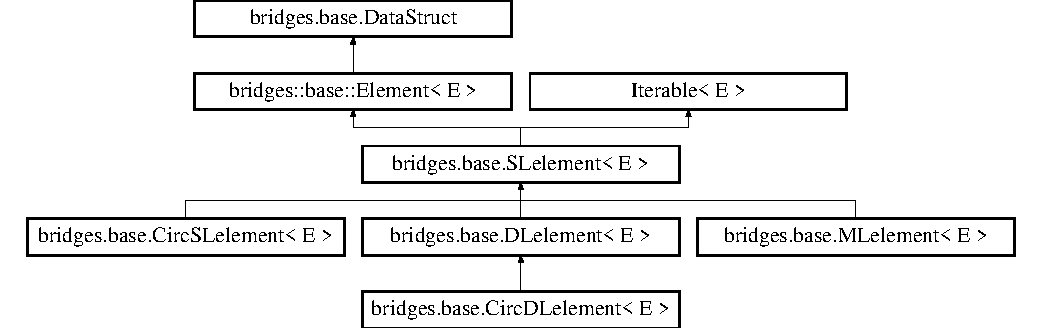
\includegraphics[height=4.000000cm]{classbridges_1_1base_1_1_s_lelement}
\end{center}
\end{figure}
\subsection*{Public Member Functions}
\begin{DoxyCompactItemize}
\item 
\hyperlink{classbridges_1_1base_1_1_s_lelement_ab9c8a08dadd76d7e0c29d7c41cf277c4}{S\+Lelement} ()
\item 
\hyperlink{classbridges_1_1base_1_1_s_lelement_a8e32c9b9e8fc8f9f1eccb14b97e031e7}{S\+Lelement} (String label, E e)
\item 
\hyperlink{classbridges_1_1base_1_1_s_lelement_abc5e333fd2f3289eede108175908f97d}{S\+Lelement} (E e, \hyperlink{classbridges_1_1base_1_1_s_lelement}{S\+Lelement}$<$ E $>$ \hyperlink{classbridges_1_1base_1_1_s_lelement_abf61c96a74ad319d561c6952ea388e0e}{next})
\item 
\hyperlink{classbridges_1_1base_1_1_s_lelement_ab5b1c20ba1d1923fad0780052fb51c99}{S\+Lelement} (\hyperlink{classbridges_1_1base_1_1_s_lelement}{S\+Lelement}$<$ E $>$ \hyperlink{classbridges_1_1base_1_1_s_lelement_abf61c96a74ad319d561c6952ea388e0e}{next})
\item 
String \hyperlink{classbridges_1_1base_1_1_s_lelement_a8c48a2d34b238fa0ae7bf2d1ee58ea88}{get\+Data\+Struct\+Type} ()
\item 
\hyperlink{classbridges_1_1base_1_1_s_lelement}{S\+Lelement}$<$ E $>$ \hyperlink{classbridges_1_1base_1_1_s_lelement_a060c4671e05e3f20b16630343393b80d}{get\+Next} ()
\item 
void \hyperlink{classbridges_1_1base_1_1_s_lelement_afdd42f03071b2614822b73729e1a5a1a}{set\+Next} (\hyperlink{classbridges_1_1base_1_1_s_lelement}{S\+Lelement}$<$ E $>$ \hyperlink{classbridges_1_1base_1_1_s_lelement_abf61c96a74ad319d561c6952ea388e0e}{next})
\item 
String \hyperlink{classbridges_1_1base_1_1_s_lelement_af0ec4da5b29d0f5ab6ab38e91cca51f9}{to\+String} ()
\end{DoxyCompactItemize}
\subsection*{Protected Attributes}
\begin{DoxyCompactItemize}
\item 
\hyperlink{classbridges_1_1base_1_1_s_lelement}{S\+Lelement}$<$ E $>$ \hyperlink{classbridges_1_1base_1_1_s_lelement_abf61c96a74ad319d561c6952ea388e0e}{next} =null
\end{DoxyCompactItemize}
\subsection*{Additional Inherited Members}


\subsection{Detailed Description}
This class can be used to instantiate Singly List Elements. 

This class extends \hyperlink{classbridges_1_1base_1_1_element}{Element} and takes a generic parameter $<$\+E$>$ for representing application specific data.

\begin{DoxyAuthor}{Author}
Mihai Mehedint, Kalpathi Subramanian
\end{DoxyAuthor}

\begin{DoxyParams}{Parameters}
{\em $<$\+E$>$} & \\
\hline
\end{DoxyParams}


\subsection{Constructor \& Destructor Documentation}
\hypertarget{classbridges_1_1base_1_1_s_lelement_ab9c8a08dadd76d7e0c29d7c41cf277c4}{}\label{classbridges_1_1base_1_1_s_lelement_ab9c8a08dadd76d7e0c29d7c41cf277c4} 
\index{bridges\+::base\+::\+S\+Lelement@{bridges\+::base\+::\+S\+Lelement}!S\+Lelement@{S\+Lelement}}
\index{S\+Lelement@{S\+Lelement}!bridges\+::base\+::\+S\+Lelement@{bridges\+::base\+::\+S\+Lelement}}
\subsubsection{\texorpdfstring{S\+Lelement()}{SLelement()}\hspace{0.1cm}{\footnotesize\ttfamily [1/4]}}
{\footnotesize\ttfamily \hyperlink{classbridges_1_1base_1_1_s_lelement}{bridges.\+base.\+S\+Lelement}$<$ E $>$.\hyperlink{classbridges_1_1base_1_1_s_lelement}{S\+Lelement} (\begin{DoxyParamCaption}{ }\end{DoxyParamCaption})}

This constructor creates an \hyperlink{classbridges_1_1base_1_1_s_lelement}{S\+Lelement} object and sets the next pointer to null \hypertarget{classbridges_1_1base_1_1_s_lelement_a8e32c9b9e8fc8f9f1eccb14b97e031e7}{}\label{classbridges_1_1base_1_1_s_lelement_a8e32c9b9e8fc8f9f1eccb14b97e031e7} 
\index{bridges\+::base\+::\+S\+Lelement@{bridges\+::base\+::\+S\+Lelement}!S\+Lelement@{S\+Lelement}}
\index{S\+Lelement@{S\+Lelement}!bridges\+::base\+::\+S\+Lelement@{bridges\+::base\+::\+S\+Lelement}}
\subsubsection{\texorpdfstring{S\+Lelement()}{SLelement()}\hspace{0.1cm}{\footnotesize\ttfamily [2/4]}}
{\footnotesize\ttfamily \hyperlink{classbridges_1_1base_1_1_s_lelement}{bridges.\+base.\+S\+Lelement}$<$ E $>$.\hyperlink{classbridges_1_1base_1_1_s_lelement}{S\+Lelement} (\begin{DoxyParamCaption}\item[{String}]{label,  }\item[{E}]{e }\end{DoxyParamCaption})}

This constructor creates an \hyperlink{classbridges_1_1base_1_1_s_lelement}{S\+Lelement} object of value \char`\"{}e\char`\"{} and label \char`\"{}label\char`\"{} and sets the next pointer to null 
\begin{DoxyParams}{Parameters}
{\em label} & the label of \hyperlink{classbridges_1_1base_1_1_s_lelement}{S\+Lelement} that shows up on the Bridges visualization \\
\hline
{\em e} & the generic object that this \hyperlink{classbridges_1_1base_1_1_s_lelement}{S\+Lelement} will hold \\
\hline
\end{DoxyParams}
\hypertarget{classbridges_1_1base_1_1_s_lelement_abc5e333fd2f3289eede108175908f97d}{}\label{classbridges_1_1base_1_1_s_lelement_abc5e333fd2f3289eede108175908f97d} 
\index{bridges\+::base\+::\+S\+Lelement@{bridges\+::base\+::\+S\+Lelement}!S\+Lelement@{S\+Lelement}}
\index{S\+Lelement@{S\+Lelement}!bridges\+::base\+::\+S\+Lelement@{bridges\+::base\+::\+S\+Lelement}}
\subsubsection{\texorpdfstring{S\+Lelement()}{SLelement()}\hspace{0.1cm}{\footnotesize\ttfamily [3/4]}}
{\footnotesize\ttfamily \hyperlink{classbridges_1_1base_1_1_s_lelement}{bridges.\+base.\+S\+Lelement}$<$ E $>$.\hyperlink{classbridges_1_1base_1_1_s_lelement}{S\+Lelement} (\begin{DoxyParamCaption}\item[{E}]{e,  }\item[{\hyperlink{classbridges_1_1base_1_1_s_lelement}{S\+Lelement}$<$ E $>$}]{next }\end{DoxyParamCaption})}

Creates a new element with value \char`\"{}e\char`\"{} and sets the next pointer to the \hyperlink{classbridges_1_1base_1_1_s_lelement}{S\+Lelement} referenced by the \char`\"{}next\char`\"{} argument 
\begin{DoxyParams}{Parameters}
{\em e} & the generic object that this \hyperlink{classbridges_1_1base_1_1_s_lelement}{S\+Lelement} will hold \\
\hline
{\em next} & the \hyperlink{classbridges_1_1base_1_1_s_lelement}{S\+Lelement} that should be assigned to the next pointer \\
\hline
\end{DoxyParams}
\hypertarget{classbridges_1_1base_1_1_s_lelement_ab5b1c20ba1d1923fad0780052fb51c99}{}\label{classbridges_1_1base_1_1_s_lelement_ab5b1c20ba1d1923fad0780052fb51c99} 
\index{bridges\+::base\+::\+S\+Lelement@{bridges\+::base\+::\+S\+Lelement}!S\+Lelement@{S\+Lelement}}
\index{S\+Lelement@{S\+Lelement}!bridges\+::base\+::\+S\+Lelement@{bridges\+::base\+::\+S\+Lelement}}
\subsubsection{\texorpdfstring{S\+Lelement()}{SLelement()}\hspace{0.1cm}{\footnotesize\ttfamily [4/4]}}
{\footnotesize\ttfamily \hyperlink{classbridges_1_1base_1_1_s_lelement}{bridges.\+base.\+S\+Lelement}$<$ E $>$.\hyperlink{classbridges_1_1base_1_1_s_lelement}{S\+Lelement} (\begin{DoxyParamCaption}\item[{\hyperlink{classbridges_1_1base_1_1_s_lelement}{S\+Lelement}$<$ E $>$}]{next }\end{DoxyParamCaption})}

Creates a new element and sets the next pointer to the \hyperlink{classbridges_1_1base_1_1_s_lelement}{S\+Lelement} \char`\"{}next\char`\"{} 
\begin{DoxyParams}{Parameters}
{\em next} & the \hyperlink{classbridges_1_1base_1_1_s_lelement}{S\+Lelement} that should be assigned to the next pointer \\
\hline
\end{DoxyParams}


\subsection{Member Function Documentation}
\hypertarget{classbridges_1_1base_1_1_s_lelement_a8c48a2d34b238fa0ae7bf2d1ee58ea88}{}\label{classbridges_1_1base_1_1_s_lelement_a8c48a2d34b238fa0ae7bf2d1ee58ea88} 
\index{bridges\+::base\+::\+S\+Lelement@{bridges\+::base\+::\+S\+Lelement}!get\+Data\+Struct\+Type@{get\+Data\+Struct\+Type}}
\index{get\+Data\+Struct\+Type@{get\+Data\+Struct\+Type}!bridges\+::base\+::\+S\+Lelement@{bridges\+::base\+::\+S\+Lelement}}
\subsubsection{\texorpdfstring{get\+Data\+Struct\+Type()}{getDataStructType()}}
{\footnotesize\ttfamily String \hyperlink{classbridges_1_1base_1_1_s_lelement}{bridges.\+base.\+S\+Lelement}$<$ E $>$.get\+Data\+Struct\+Type (\begin{DoxyParamCaption}{ }\end{DoxyParamCaption})}

This method gets the data structure type

\begin{DoxyReturn}{Returns}
The date structure type as a string 
\end{DoxyReturn}
\hypertarget{classbridges_1_1base_1_1_s_lelement_a060c4671e05e3f20b16630343393b80d}{}\label{classbridges_1_1base_1_1_s_lelement_a060c4671e05e3f20b16630343393b80d} 
\index{bridges\+::base\+::\+S\+Lelement@{bridges\+::base\+::\+S\+Lelement}!get\+Next@{get\+Next}}
\index{get\+Next@{get\+Next}!bridges\+::base\+::\+S\+Lelement@{bridges\+::base\+::\+S\+Lelement}}
\subsubsection{\texorpdfstring{get\+Next()}{getNext()}}
{\footnotesize\ttfamily \hyperlink{classbridges_1_1base_1_1_s_lelement}{S\+Lelement}$<$E$>$ \hyperlink{classbridges_1_1base_1_1_s_lelement}{bridges.\+base.\+S\+Lelement}$<$ E $>$.get\+Next (\begin{DoxyParamCaption}{ }\end{DoxyParamCaption})}

Retrieves the next \hyperlink{classbridges_1_1base_1_1_s_lelement}{S\+Lelement} \begin{DoxyReturn}{Returns}
S\+Lelement$<$\+E$>$ assigned to next 
\end{DoxyReturn}
\hypertarget{classbridges_1_1base_1_1_s_lelement_afdd42f03071b2614822b73729e1a5a1a}{}\label{classbridges_1_1base_1_1_s_lelement_afdd42f03071b2614822b73729e1a5a1a} 
\index{bridges\+::base\+::\+S\+Lelement@{bridges\+::base\+::\+S\+Lelement}!set\+Next@{set\+Next}}
\index{set\+Next@{set\+Next}!bridges\+::base\+::\+S\+Lelement@{bridges\+::base\+::\+S\+Lelement}}
\subsubsection{\texorpdfstring{set\+Next()}{setNext()}}
{\footnotesize\ttfamily void \hyperlink{classbridges_1_1base_1_1_s_lelement}{bridges.\+base.\+S\+Lelement}$<$ E $>$.set\+Next (\begin{DoxyParamCaption}\item[{\hyperlink{classbridges_1_1base_1_1_s_lelement}{S\+Lelement}$<$ E $>$}]{next }\end{DoxyParamCaption})}

Sets the pointer to the next \hyperlink{classbridges_1_1base_1_1_s_lelement}{S\+Lelement} 
\begin{DoxyParams}{Parameters}
{\em next} & S\+Lelement$<$\+E$>$ that should be assigned to the next pointer \\
\hline
\end{DoxyParams}
\hypertarget{classbridges_1_1base_1_1_s_lelement_af0ec4da5b29d0f5ab6ab38e91cca51f9}{}\label{classbridges_1_1base_1_1_s_lelement_af0ec4da5b29d0f5ab6ab38e91cca51f9} 
\index{bridges\+::base\+::\+S\+Lelement@{bridges\+::base\+::\+S\+Lelement}!to\+String@{to\+String}}
\index{to\+String@{to\+String}!bridges\+::base\+::\+S\+Lelement@{bridges\+::base\+::\+S\+Lelement}}
\subsubsection{\texorpdfstring{to\+String()}{toString()}}
{\footnotesize\ttfamily String \hyperlink{classbridges_1_1base_1_1_s_lelement}{bridges.\+base.\+S\+Lelement}$<$ E $>$.to\+String (\begin{DoxyParamCaption}{ }\end{DoxyParamCaption})}



\subsection{Member Data Documentation}
\hypertarget{classbridges_1_1base_1_1_s_lelement_abf61c96a74ad319d561c6952ea388e0e}{}\label{classbridges_1_1base_1_1_s_lelement_abf61c96a74ad319d561c6952ea388e0e} 
\index{bridges\+::base\+::\+S\+Lelement@{bridges\+::base\+::\+S\+Lelement}!next@{next}}
\index{next@{next}!bridges\+::base\+::\+S\+Lelement@{bridges\+::base\+::\+S\+Lelement}}
\subsubsection{\texorpdfstring{next}{next}}
{\footnotesize\ttfamily \hyperlink{classbridges_1_1base_1_1_s_lelement}{S\+Lelement}$<$E$>$ \hyperlink{classbridges_1_1base_1_1_s_lelement}{bridges.\+base.\+S\+Lelement}$<$ E $>$.next =null\hspace{0.3cm}{\ttfamily [protected]}}



The documentation for this class was generated from the following file\+:\begin{DoxyCompactItemize}
\item 
link/base/\hyperlink{_s_lelement_8java}{S\+Lelement.\+java}\end{DoxyCompactItemize}

\hypertarget{classbridges_1_1connect_1_1_socket_connection}{}\section{bridges.\+connect.\+Socket\+Connection Class Reference}
\label{classbridges_1_1connect_1_1_socket_connection}\index{bridges.\+connect.\+Socket\+Connection@{bridges.\+connect.\+Socket\+Connection}}
\subsection*{Public Member Functions}
\begin{DoxyCompactItemize}
\item 
\hyperlink{classbridges_1_1connect_1_1_socket_connection_a876856ccf07a3ae6519d7f7b94d0e65a}{Socket\+Connection} (\hyperlink{classbridges_1_1connect_1_1_bridges}{Bridges} b)
\item 
void \hyperlink{classbridges_1_1connect_1_1_socket_connection_a94dd56d930f24abf547bce3ad0fb723e}{add\+Listener} (\hyperlink{interfacebridges_1_1connect_1_1_keypress_listener}{Keypress\+Listener} to\+Add)
\item 
void \hyperlink{classbridges_1_1connect_1_1_socket_connection_ac5467b4da6cd41b0cee00be5b4cbc60d}{setup\+Connection} ()
\item 
void \hyperlink{classbridges_1_1connect_1_1_socket_connection_a9f62a8dbff3debd6d226f9a0d59a4c33}{send\+Data} (String dataframe)
\item 
void \hyperlink{classbridges_1_1connect_1_1_socket_connection_aeb96c978c1dd5125f3068ecc7c79e3ca}{close} ()
\end{DoxyCompactItemize}


\subsection{Constructor \& Destructor Documentation}
\mbox{\Hypertarget{classbridges_1_1connect_1_1_socket_connection_a876856ccf07a3ae6519d7f7b94d0e65a}\label{classbridges_1_1connect_1_1_socket_connection_a876856ccf07a3ae6519d7f7b94d0e65a}} 
\index{bridges\+::connect\+::\+Socket\+Connection@{bridges\+::connect\+::\+Socket\+Connection}!Socket\+Connection@{Socket\+Connection}}
\index{Socket\+Connection@{Socket\+Connection}!bridges\+::connect\+::\+Socket\+Connection@{bridges\+::connect\+::\+Socket\+Connection}}
\subsubsection{\texorpdfstring{Socket\+Connection()}{SocketConnection()}}
{\footnotesize\ttfamily bridges.\+connect.\+Socket\+Connection.\+Socket\+Connection (\begin{DoxyParamCaption}\item[{\hyperlink{classbridges_1_1connect_1_1_bridges}{Bridges}}]{b }\end{DoxyParamCaption})}



\subsection{Member Function Documentation}
\mbox{\Hypertarget{classbridges_1_1connect_1_1_socket_connection_a94dd56d930f24abf547bce3ad0fb723e}\label{classbridges_1_1connect_1_1_socket_connection_a94dd56d930f24abf547bce3ad0fb723e}} 
\index{bridges\+::connect\+::\+Socket\+Connection@{bridges\+::connect\+::\+Socket\+Connection}!add\+Listener@{add\+Listener}}
\index{add\+Listener@{add\+Listener}!bridges\+::connect\+::\+Socket\+Connection@{bridges\+::connect\+::\+Socket\+Connection}}
\subsubsection{\texorpdfstring{add\+Listener()}{addListener()}}
{\footnotesize\ttfamily void bridges.\+connect.\+Socket\+Connection.\+add\+Listener (\begin{DoxyParamCaption}\item[{\hyperlink{interfacebridges_1_1connect_1_1_keypress_listener}{Keypress\+Listener}}]{to\+Add }\end{DoxyParamCaption})}

\mbox{\Hypertarget{classbridges_1_1connect_1_1_socket_connection_aeb96c978c1dd5125f3068ecc7c79e3ca}\label{classbridges_1_1connect_1_1_socket_connection_aeb96c978c1dd5125f3068ecc7c79e3ca}} 
\index{bridges\+::connect\+::\+Socket\+Connection@{bridges\+::connect\+::\+Socket\+Connection}!close@{close}}
\index{close@{close}!bridges\+::connect\+::\+Socket\+Connection@{bridges\+::connect\+::\+Socket\+Connection}}
\subsubsection{\texorpdfstring{close()}{close()}}
{\footnotesize\ttfamily void bridges.\+connect.\+Socket\+Connection.\+close (\begin{DoxyParamCaption}{ }\end{DoxyParamCaption})}

\mbox{\Hypertarget{classbridges_1_1connect_1_1_socket_connection_a9f62a8dbff3debd6d226f9a0d59a4c33}\label{classbridges_1_1connect_1_1_socket_connection_a9f62a8dbff3debd6d226f9a0d59a4c33}} 
\index{bridges\+::connect\+::\+Socket\+Connection@{bridges\+::connect\+::\+Socket\+Connection}!send\+Data@{send\+Data}}
\index{send\+Data@{send\+Data}!bridges\+::connect\+::\+Socket\+Connection@{bridges\+::connect\+::\+Socket\+Connection}}
\subsubsection{\texorpdfstring{send\+Data()}{sendData()}}
{\footnotesize\ttfamily void bridges.\+connect.\+Socket\+Connection.\+send\+Data (\begin{DoxyParamCaption}\item[{String}]{dataframe }\end{DoxyParamCaption})}

\mbox{\Hypertarget{classbridges_1_1connect_1_1_socket_connection_ac5467b4da6cd41b0cee00be5b4cbc60d}\label{classbridges_1_1connect_1_1_socket_connection_ac5467b4da6cd41b0cee00be5b4cbc60d}} 
\index{bridges\+::connect\+::\+Socket\+Connection@{bridges\+::connect\+::\+Socket\+Connection}!setup\+Connection@{setup\+Connection}}
\index{setup\+Connection@{setup\+Connection}!bridges\+::connect\+::\+Socket\+Connection@{bridges\+::connect\+::\+Socket\+Connection}}
\subsubsection{\texorpdfstring{setup\+Connection()}{setupConnection()}}
{\footnotesize\ttfamily void bridges.\+connect.\+Socket\+Connection.\+setup\+Connection (\begin{DoxyParamCaption}{ }\end{DoxyParamCaption})}



The documentation for this class was generated from the following file\+:\begin{DoxyCompactItemize}
\item 
/home/erik/work/bridges/bridges-\/java/src/main/java/bridges/connect/\hyperlink{_socket_connection_8java}{Socket\+Connection.\+java}\end{DoxyCompactItemize}

\hypertarget{classbridges_1_1data__src__dependent_1_1_song}{}\section{bridges.\+data\+\_\+src\+\_\+dependent.\+Song Class Reference}
\label{classbridges_1_1data__src__dependent_1_1_song}\index{bridges.\+data\+\_\+src\+\_\+dependent.\+Song@{bridges.\+data\+\_\+src\+\_\+dependent.\+Song}}
\subsection*{Public Member Functions}
\begin{DoxyCompactItemize}
\item 
\hyperlink{classbridges_1_1data__src__dependent_1_1_song_a824052caca0b9c03d07c42e9e7740020}{Song} ()
\item 
\hyperlink{classbridges_1_1data__src__dependent_1_1_song_a78506e63f4d91dc1f0d821050a093ad6}{Song} (String artist, String song, String album, String lyrics, String release\+\_\+date)
\item 
String \hyperlink{classbridges_1_1data__src__dependent_1_1_song_a7aa3685df74e4fbb5e0d4d4750cf7685}{get\+Artist} ()
\item 
void \hyperlink{classbridges_1_1data__src__dependent_1_1_song_adffaec742bf945ec8c81244fdafd47d2}{set\+Artist} (String artist)
\item 
String \hyperlink{classbridges_1_1data__src__dependent_1_1_song_a4e7b8aed1aec243f2798a30e51091d72}{get\+Song\+Title} ()
\item 
void \hyperlink{classbridges_1_1data__src__dependent_1_1_song_a9d7540c0e6cca53ae3a105885aac5622}{set\+Song\+Title} (String song)
\item 
String \hyperlink{classbridges_1_1data__src__dependent_1_1_song_a94b26a355aa1e30938bcc896a8bd902f}{get\+Album\+Title} ()
\item 
void \hyperlink{classbridges_1_1data__src__dependent_1_1_song_ab9f9d24be49c3a0a66c9ff9e271b007e}{set\+Album\+Title} (String album)
\item 
String \hyperlink{classbridges_1_1data__src__dependent_1_1_song_ab4aa2c51f7fdce80d9c178d6f0e0aae8}{get\+Lyrics} ()
\item 
void \hyperlink{classbridges_1_1data__src__dependent_1_1_song_a30889eb971f474e9d62782ddb82c1846}{set\+Lyrics} (String lyrics)
\item 
String \hyperlink{classbridges_1_1data__src__dependent_1_1_song_a05520675a0a2f2e60583887b8c69cde4}{get\+Release\+Date} ()
\item 
void \hyperlink{classbridges_1_1data__src__dependent_1_1_song_a6534e543a295b29858cf98be7a4e276e}{set\+Release\+Date} (String release\+\_\+date)
\end{DoxyCompactItemize}


\subsection{Constructor \& Destructor Documentation}
\mbox{\Hypertarget{classbridges_1_1data__src__dependent_1_1_song_a824052caca0b9c03d07c42e9e7740020}\label{classbridges_1_1data__src__dependent_1_1_song_a824052caca0b9c03d07c42e9e7740020}} 
\index{bridges\+::data\+\_\+src\+\_\+dependent\+::\+Song@{bridges\+::data\+\_\+src\+\_\+dependent\+::\+Song}!Song@{Song}}
\index{Song@{Song}!bridges\+::data\+\_\+src\+\_\+dependent\+::\+Song@{bridges\+::data\+\_\+src\+\_\+dependent\+::\+Song}}
\subsubsection{\texorpdfstring{Song()}{Song()}\hspace{0.1cm}{\footnotesize\ttfamily [1/2]}}
{\footnotesize\ttfamily bridges.\+data\+\_\+src\+\_\+dependent.\+Song.\+Song (\begin{DoxyParamCaption}{ }\end{DoxyParamCaption})}

\hyperlink{classbridges_1_1data__src__dependent_1_1_song}{Song} constructors \mbox{\Hypertarget{classbridges_1_1data__src__dependent_1_1_song_a78506e63f4d91dc1f0d821050a093ad6}\label{classbridges_1_1data__src__dependent_1_1_song_a78506e63f4d91dc1f0d821050a093ad6}} 
\index{bridges\+::data\+\_\+src\+\_\+dependent\+::\+Song@{bridges\+::data\+\_\+src\+\_\+dependent\+::\+Song}!Song@{Song}}
\index{Song@{Song}!bridges\+::data\+\_\+src\+\_\+dependent\+::\+Song@{bridges\+::data\+\_\+src\+\_\+dependent\+::\+Song}}
\subsubsection{\texorpdfstring{Song()}{Song()}\hspace{0.1cm}{\footnotesize\ttfamily [2/2]}}
{\footnotesize\ttfamily bridges.\+data\+\_\+src\+\_\+dependent.\+Song.\+Song (\begin{DoxyParamCaption}\item[{String}]{artist,  }\item[{String}]{song,  }\item[{String}]{album,  }\item[{String}]{lyrics,  }\item[{String}]{release\+\_\+date }\end{DoxyParamCaption})}

\hyperlink{classbridges_1_1data__src__dependent_1_1_song}{Song} constructor


\begin{DoxyParams}{Parameters}
{\em artist} & artist of song \\
\hline
{\em song} & song title \\
\hline
{\em album} & album title \\
\hline
{\em lyrics} & lyrics of song (string) \\
\hline
{\em release\+\_\+date} & date released \\
\hline
\end{DoxyParams}


\subsection{Member Function Documentation}
\mbox{\Hypertarget{classbridges_1_1data__src__dependent_1_1_song_a94b26a355aa1e30938bcc896a8bd902f}\label{classbridges_1_1data__src__dependent_1_1_song_a94b26a355aa1e30938bcc896a8bd902f}} 
\index{bridges\+::data\+\_\+src\+\_\+dependent\+::\+Song@{bridges\+::data\+\_\+src\+\_\+dependent\+::\+Song}!get\+Album\+Title@{get\+Album\+Title}}
\index{get\+Album\+Title@{get\+Album\+Title}!bridges\+::data\+\_\+src\+\_\+dependent\+::\+Song@{bridges\+::data\+\_\+src\+\_\+dependent\+::\+Song}}
\subsubsection{\texorpdfstring{get\+Album\+Title()}{getAlbumTitle()}}
{\footnotesize\ttfamily String bridges.\+data\+\_\+src\+\_\+dependent.\+Song.\+get\+Album\+Title (\begin{DoxyParamCaption}{ }\end{DoxyParamCaption})}

Get album title containing the song \begin{DoxyReturn}{Returns}
album title (string) 
\end{DoxyReturn}
\mbox{\Hypertarget{classbridges_1_1data__src__dependent_1_1_song_a7aa3685df74e4fbb5e0d4d4750cf7685}\label{classbridges_1_1data__src__dependent_1_1_song_a7aa3685df74e4fbb5e0d4d4750cf7685}} 
\index{bridges\+::data\+\_\+src\+\_\+dependent\+::\+Song@{bridges\+::data\+\_\+src\+\_\+dependent\+::\+Song}!get\+Artist@{get\+Artist}}
\index{get\+Artist@{get\+Artist}!bridges\+::data\+\_\+src\+\_\+dependent\+::\+Song@{bridges\+::data\+\_\+src\+\_\+dependent\+::\+Song}}
\subsubsection{\texorpdfstring{get\+Artist()}{getArtist()}}
{\footnotesize\ttfamily String bridges.\+data\+\_\+src\+\_\+dependent.\+Song.\+get\+Artist (\begin{DoxyParamCaption}{ }\end{DoxyParamCaption})}

Get song artist \begin{DoxyReturn}{Returns}
artist of song 
\end{DoxyReturn}
\mbox{\Hypertarget{classbridges_1_1data__src__dependent_1_1_song_ab4aa2c51f7fdce80d9c178d6f0e0aae8}\label{classbridges_1_1data__src__dependent_1_1_song_ab4aa2c51f7fdce80d9c178d6f0e0aae8}} 
\index{bridges\+::data\+\_\+src\+\_\+dependent\+::\+Song@{bridges\+::data\+\_\+src\+\_\+dependent\+::\+Song}!get\+Lyrics@{get\+Lyrics}}
\index{get\+Lyrics@{get\+Lyrics}!bridges\+::data\+\_\+src\+\_\+dependent\+::\+Song@{bridges\+::data\+\_\+src\+\_\+dependent\+::\+Song}}
\subsubsection{\texorpdfstring{get\+Lyrics()}{getLyrics()}}
{\footnotesize\ttfamily String bridges.\+data\+\_\+src\+\_\+dependent.\+Song.\+get\+Lyrics (\begin{DoxyParamCaption}{ }\end{DoxyParamCaption})}

Get lyrics of the song \begin{DoxyReturn}{Returns}
lyrics of song (string) 
\end{DoxyReturn}
\mbox{\Hypertarget{classbridges_1_1data__src__dependent_1_1_song_a05520675a0a2f2e60583887b8c69cde4}\label{classbridges_1_1data__src__dependent_1_1_song_a05520675a0a2f2e60583887b8c69cde4}} 
\index{bridges\+::data\+\_\+src\+\_\+dependent\+::\+Song@{bridges\+::data\+\_\+src\+\_\+dependent\+::\+Song}!get\+Release\+Date@{get\+Release\+Date}}
\index{get\+Release\+Date@{get\+Release\+Date}!bridges\+::data\+\_\+src\+\_\+dependent\+::\+Song@{bridges\+::data\+\_\+src\+\_\+dependent\+::\+Song}}
\subsubsection{\texorpdfstring{get\+Release\+Date()}{getReleaseDate()}}
{\footnotesize\ttfamily String bridges.\+data\+\_\+src\+\_\+dependent.\+Song.\+get\+Release\+Date (\begin{DoxyParamCaption}{ }\end{DoxyParamCaption})}

Get release date of the song \begin{DoxyReturn}{Returns}
release date of song (string) 
\end{DoxyReturn}
\mbox{\Hypertarget{classbridges_1_1data__src__dependent_1_1_song_a4e7b8aed1aec243f2798a30e51091d72}\label{classbridges_1_1data__src__dependent_1_1_song_a4e7b8aed1aec243f2798a30e51091d72}} 
\index{bridges\+::data\+\_\+src\+\_\+dependent\+::\+Song@{bridges\+::data\+\_\+src\+\_\+dependent\+::\+Song}!get\+Song\+Title@{get\+Song\+Title}}
\index{get\+Song\+Title@{get\+Song\+Title}!bridges\+::data\+\_\+src\+\_\+dependent\+::\+Song@{bridges\+::data\+\_\+src\+\_\+dependent\+::\+Song}}
\subsubsection{\texorpdfstring{get\+Song\+Title()}{getSongTitle()}}
{\footnotesize\ttfamily String bridges.\+data\+\_\+src\+\_\+dependent.\+Song.\+get\+Song\+Title (\begin{DoxyParamCaption}{ }\end{DoxyParamCaption})}

Get song title \begin{DoxyReturn}{Returns}
title of song (string) 
\end{DoxyReturn}
\mbox{\Hypertarget{classbridges_1_1data__src__dependent_1_1_song_ab9f9d24be49c3a0a66c9ff9e271b007e}\label{classbridges_1_1data__src__dependent_1_1_song_ab9f9d24be49c3a0a66c9ff9e271b007e}} 
\index{bridges\+::data\+\_\+src\+\_\+dependent\+::\+Song@{bridges\+::data\+\_\+src\+\_\+dependent\+::\+Song}!set\+Album\+Title@{set\+Album\+Title}}
\index{set\+Album\+Title@{set\+Album\+Title}!bridges\+::data\+\_\+src\+\_\+dependent\+::\+Song@{bridges\+::data\+\_\+src\+\_\+dependent\+::\+Song}}
\subsubsection{\texorpdfstring{set\+Album\+Title()}{setAlbumTitle()}}
{\footnotesize\ttfamily void bridges.\+data\+\_\+src\+\_\+dependent.\+Song.\+set\+Album\+Title (\begin{DoxyParamCaption}\item[{String}]{album }\end{DoxyParamCaption})}

Set song album 
\begin{DoxyParams}{Parameters}
{\em album} & song album to set \\
\hline
\end{DoxyParams}
\mbox{\Hypertarget{classbridges_1_1data__src__dependent_1_1_song_adffaec742bf945ec8c81244fdafd47d2}\label{classbridges_1_1data__src__dependent_1_1_song_adffaec742bf945ec8c81244fdafd47d2}} 
\index{bridges\+::data\+\_\+src\+\_\+dependent\+::\+Song@{bridges\+::data\+\_\+src\+\_\+dependent\+::\+Song}!set\+Artist@{set\+Artist}}
\index{set\+Artist@{set\+Artist}!bridges\+::data\+\_\+src\+\_\+dependent\+::\+Song@{bridges\+::data\+\_\+src\+\_\+dependent\+::\+Song}}
\subsubsection{\texorpdfstring{set\+Artist()}{setArtist()}}
{\footnotesize\ttfamily void bridges.\+data\+\_\+src\+\_\+dependent.\+Song.\+set\+Artist (\begin{DoxyParamCaption}\item[{String}]{artist }\end{DoxyParamCaption})}

Set song artist 
\begin{DoxyParams}{Parameters}
{\em artist} & artist to set \\
\hline
\end{DoxyParams}
\mbox{\Hypertarget{classbridges_1_1data__src__dependent_1_1_song_a30889eb971f474e9d62782ddb82c1846}\label{classbridges_1_1data__src__dependent_1_1_song_a30889eb971f474e9d62782ddb82c1846}} 
\index{bridges\+::data\+\_\+src\+\_\+dependent\+::\+Song@{bridges\+::data\+\_\+src\+\_\+dependent\+::\+Song}!set\+Lyrics@{set\+Lyrics}}
\index{set\+Lyrics@{set\+Lyrics}!bridges\+::data\+\_\+src\+\_\+dependent\+::\+Song@{bridges\+::data\+\_\+src\+\_\+dependent\+::\+Song}}
\subsubsection{\texorpdfstring{set\+Lyrics()}{setLyrics()}}
{\footnotesize\ttfamily void bridges.\+data\+\_\+src\+\_\+dependent.\+Song.\+set\+Lyrics (\begin{DoxyParamCaption}\item[{String}]{lyrics }\end{DoxyParamCaption})}

Set song lyrics 
\begin{DoxyParams}{Parameters}
{\em lyrics} & of song to set \\
\hline
\end{DoxyParams}
\mbox{\Hypertarget{classbridges_1_1data__src__dependent_1_1_song_a6534e543a295b29858cf98be7a4e276e}\label{classbridges_1_1data__src__dependent_1_1_song_a6534e543a295b29858cf98be7a4e276e}} 
\index{bridges\+::data\+\_\+src\+\_\+dependent\+::\+Song@{bridges\+::data\+\_\+src\+\_\+dependent\+::\+Song}!set\+Release\+Date@{set\+Release\+Date}}
\index{set\+Release\+Date@{set\+Release\+Date}!bridges\+::data\+\_\+src\+\_\+dependent\+::\+Song@{bridges\+::data\+\_\+src\+\_\+dependent\+::\+Song}}
\subsubsection{\texorpdfstring{set\+Release\+Date()}{setReleaseDate()}}
{\footnotesize\ttfamily void bridges.\+data\+\_\+src\+\_\+dependent.\+Song.\+set\+Release\+Date (\begin{DoxyParamCaption}\item[{String}]{release\+\_\+date }\end{DoxyParamCaption})}

Set release date of song 
\begin{DoxyParams}{Parameters}
{\em release\+\_\+date} & date of release to set \\
\hline
\end{DoxyParams}
\mbox{\Hypertarget{classbridges_1_1data__src__dependent_1_1_song_a9d7540c0e6cca53ae3a105885aac5622}\label{classbridges_1_1data__src__dependent_1_1_song_a9d7540c0e6cca53ae3a105885aac5622}} 
\index{bridges\+::data\+\_\+src\+\_\+dependent\+::\+Song@{bridges\+::data\+\_\+src\+\_\+dependent\+::\+Song}!set\+Song\+Title@{set\+Song\+Title}}
\index{set\+Song\+Title@{set\+Song\+Title}!bridges\+::data\+\_\+src\+\_\+dependent\+::\+Song@{bridges\+::data\+\_\+src\+\_\+dependent\+::\+Song}}
\subsubsection{\texorpdfstring{set\+Song\+Title()}{setSongTitle()}}
{\footnotesize\ttfamily void bridges.\+data\+\_\+src\+\_\+dependent.\+Song.\+set\+Song\+Title (\begin{DoxyParamCaption}\item[{String}]{song }\end{DoxyParamCaption})}

Set song title 
\begin{DoxyParams}{Parameters}
{\em song} & song title to set \\
\hline
\end{DoxyParams}


The documentation for this class was generated from the following file\+:\begin{DoxyCompactItemize}
\item 
/home/erik/work/bridges/bridges-\/java/src/main/java/bridges/data\+\_\+src\+\_\+dependent/\hyperlink{_song_8java}{Song.\+java}\end{DoxyCompactItemize}

\hypertarget{classbridges_1_1benchmark_1_1_sorting_benchmark}{}\section{bridges\+::benchmark\+::Sorting\+Benchmark Class Reference}
\label{classbridges_1_1benchmark_1_1_sorting_benchmark}\index{bridges::benchmark::SortingBenchmark@{bridges::benchmark::SortingBenchmark}}


{\ttfamily \#include $<$Sorting\+Benchmark.\+h$>$}



\subsection{Detailed Description}
Benchmarks sorting algorithm. 

Benchmarks sorting algorithms and add time series to a Line\+Chart.

The benchmark goes from an initial size controlled by \mbox{\hyperlink{classbridges_1_1benchmark_1_1_sorting_benchmark_afe0474d148c185ed1e479ff11f42ae51}{set\+Base\+Size()}} to a largest size controlled by \mbox{\hyperlink{classbridges_1_1benchmark_1_1_sorting_benchmark_abdca289b823c7f240b648e248c07b059}{set\+Max\+Size()}}. One can also set a maximum time spent on a particular run using \mbox{\hyperlink{classbridges_1_1benchmark_1_1_sorting_benchmark_a59b95f2510d62ac5a31bb33d472fdffc}{set\+Time\+Cap()}}.

The benchmark goes from a array size of n to the next one of geo\+Base $\ast$ n + increment, where the base is controlled by \mbox{\hyperlink{classbridges_1_1benchmark_1_1_sorting_benchmark_ade76a5749b07d35b02623cce27c046ab}{set\+Geometric()}} and increment is controlled by \mbox{\hyperlink{classbridges_1_1benchmark_1_1_sorting_benchmark_ae168533dc5756f3ede3436bdd7840047}{set\+Increment()}}. For simpler use one can set a purley linear sampling with \mbox{\hyperlink{classbridges_1_1benchmark_1_1_sorting_benchmark_a993de51c8b82ec50eb186afef5dc7003}{linear\+Range()}} or a purely geometric one with \mbox{\hyperlink{classbridges_1_1benchmark_1_1_sorting_benchmark_a32fa712ee712b633aabfd7bcaa83008a}{geometric\+Range()}}.

The sorting algorithms must have for prototype\+: void ({\itshape sort)(int} array, int arraysize); and can be passed to the run function for being benchmarked. A typical use would look something like


\begin{DoxyCode}{0}
\DoxyCodeLine{\textcolor{keywordtype}{void} mysort(\textcolor{keywordtype}{int}* array, \textcolor{keywordtype}{int} arraysize);}
\DoxyCodeLine{LineChart lc;}
\DoxyCodeLine{\mbox{\hyperlink{classbridges_1_1benchmark_1_1_sorting_benchmark_aed5731a3b5add3a7f4c80891b22b3093}{SortingBenchmark}} sb (lc);}
\DoxyCodeLine{sb.linearRange (100, 1000, 5);}
\DoxyCodeLine{sb.run(\textcolor{stringliteral}{"mysortingalgorithm"}, mysort);}
\end{DoxyCode}


\begin{DoxyAuthor}{Author}
Erik Saule 
\end{DoxyAuthor}
\begin{DoxyDate}{Date}
07/20/2019 
\end{DoxyDate}
\subsection*{Public Member Functions}
\begin{DoxyCompactItemize}
\item 
\mbox{\hyperlink{classbridges_1_1benchmark_1_1_sorting_benchmark_aed5731a3b5add3a7f4c80891b22b3093}{Sorting\+Benchmark}} (\mbox{\hyperlink{classbridges_1_1datastructure_1_1_line_chart}{Line\+Chart}} \&p)
\item 
void \mbox{\hyperlink{classbridges_1_1benchmark_1_1_sorting_benchmark_abdca289b823c7f240b648e248c07b059}{set\+Max\+Size}} (int size)
\begin{DoxyCompactList}\small\item\em Puts a cap on the largest array to be used. \end{DoxyCompactList}\item 
void \mbox{\hyperlink{classbridges_1_1benchmark_1_1_sorting_benchmark_afe0474d148c185ed1e479ff11f42ae51}{set\+Base\+Size}} (int size)
\begin{DoxyCompactList}\small\item\em Smallest array to be used. \end{DoxyCompactList}\item 
void \mbox{\hyperlink{classbridges_1_1benchmark_1_1_sorting_benchmark_ae168533dc5756f3ede3436bdd7840047}{set\+Increment}} (int inc)
\begin{DoxyCompactList}\small\item\em Sets the increment for the benchmark size. \end{DoxyCompactList}\item 
void \mbox{\hyperlink{classbridges_1_1benchmark_1_1_sorting_benchmark_ade76a5749b07d35b02623cce27c046ab}{set\+Geometric}} (double base)
\begin{DoxyCompactList}\small\item\em Sets a geometric progression for the benchmark size. \end{DoxyCompactList}\item 
void \mbox{\hyperlink{classbridges_1_1benchmark_1_1_sorting_benchmark_a993de51c8b82ec50eb186afef5dc7003}{linear\+Range}} (int base\+Size, int max\+Size, int nb\+Point)
\begin{DoxyCompactList}\small\item\em The benchmark will sample a range with a fixed number of points. \end{DoxyCompactList}\item 
void \mbox{\hyperlink{classbridges_1_1benchmark_1_1_sorting_benchmark_a32fa712ee712b633aabfd7bcaa83008a}{geometric\+Range}} (int base\+Size, int max\+Size, double base)
\begin{DoxyCompactList}\small\item\em The benchmark will sample a range using in geometrically increasing sequence. \end{DoxyCompactList}\item 
void \mbox{\hyperlink{classbridges_1_1benchmark_1_1_sorting_benchmark_a59b95f2510d62ac5a31bb33d472fdffc}{set\+Time\+Cap}} (double cap\+\_\+in\+\_\+s)
\begin{DoxyCompactList}\small\item\em sets an upper bound to the time of a run. \end{DoxyCompactList}\item 
void \mbox{\hyperlink{classbridges_1_1benchmark_1_1_sorting_benchmark_a790e43dd840f6787286133eedec32628}{run}} (std\+::string algo\+Name, void($\ast$runnable)(int $\ast$, int))
\begin{DoxyCompactList}\small\item\em benchmark one implementation \end{DoxyCompactList}\end{DoxyCompactItemize}


\subsection{Constructor \& Destructor Documentation}
\mbox{\Hypertarget{classbridges_1_1benchmark_1_1_sorting_benchmark_aed5731a3b5add3a7f4c80891b22b3093}\label{classbridges_1_1benchmark_1_1_sorting_benchmark_aed5731a3b5add3a7f4c80891b22b3093}} 
\index{bridges::benchmark::SortingBenchmark@{bridges::benchmark::SortingBenchmark}!SortingBenchmark@{SortingBenchmark}}
\index{SortingBenchmark@{SortingBenchmark}!bridges::benchmark::SortingBenchmark@{bridges::benchmark::SortingBenchmark}}
\subsubsection{\texorpdfstring{SortingBenchmark()}{SortingBenchmark()}}
{\footnotesize\ttfamily bridges\+::benchmark\+::\+Sorting\+Benchmark\+::\+Sorting\+Benchmark (\begin{DoxyParamCaption}\item[{\mbox{\hyperlink{classbridges_1_1datastructure_1_1_line_chart}{Line\+Chart}} \&}]{p }\end{DoxyParamCaption})\hspace{0.3cm}{\ttfamily [inline]}}



\subsection{Member Function Documentation}
\mbox{\Hypertarget{classbridges_1_1benchmark_1_1_sorting_benchmark_a32fa712ee712b633aabfd7bcaa83008a}\label{classbridges_1_1benchmark_1_1_sorting_benchmark_a32fa712ee712b633aabfd7bcaa83008a}} 
\index{bridges::benchmark::SortingBenchmark@{bridges::benchmark::SortingBenchmark}!geometricRange@{geometricRange}}
\index{geometricRange@{geometricRange}!bridges::benchmark::SortingBenchmark@{bridges::benchmark::SortingBenchmark}}
\subsubsection{\texorpdfstring{geometricRange()}{geometricRange()}}
{\footnotesize\ttfamily void bridges\+::benchmark\+::\+Sorting\+Benchmark\+::geometric\+Range (\begin{DoxyParamCaption}\item[{int}]{base\+Size,  }\item[{int}]{max\+Size,  }\item[{double}]{base }\end{DoxyParamCaption})\hspace{0.3cm}{\ttfamily [inline]}}



The benchmark will sample a range using in geometrically increasing sequence. 

The benchmark will sample the range \mbox{[}base\+Size; max\+Size\mbox{]} using a geometric distribution in base base. That is to say, it will sample base\+Size, base$\ast$base\+Size, base$\ast$base$\ast$base\+Size, ...


\begin{DoxyParams}{Parameters}
{\em base\+Size} & lower bound of the range sampled \\
\hline
{\em max\+Size} & upper bound of the range sampled \\
\hline
{\em base} & base of the geometric increase \\
\hline
\end{DoxyParams}
\mbox{\Hypertarget{classbridges_1_1benchmark_1_1_sorting_benchmark_a993de51c8b82ec50eb186afef5dc7003}\label{classbridges_1_1benchmark_1_1_sorting_benchmark_a993de51c8b82ec50eb186afef5dc7003}} 
\index{bridges::benchmark::SortingBenchmark@{bridges::benchmark::SortingBenchmark}!linearRange@{linearRange}}
\index{linearRange@{linearRange}!bridges::benchmark::SortingBenchmark@{bridges::benchmark::SortingBenchmark}}
\subsubsection{\texorpdfstring{linearRange()}{linearRange()}}
{\footnotesize\ttfamily void bridges\+::benchmark\+::\+Sorting\+Benchmark\+::linear\+Range (\begin{DoxyParamCaption}\item[{int}]{base\+Size,  }\item[{int}]{max\+Size,  }\item[{int}]{nb\+Point }\end{DoxyParamCaption})\hspace{0.3cm}{\ttfamily [inline]}}



The benchmark will sample a range with a fixed number of points. 

The benchmark will sample about nb\+Point equally distributed in the range \mbox{[}base\+Size; max\+Size\mbox{]}


\begin{DoxyParams}{Parameters}
{\em base\+Size} & lower bound of the range sampled \\
\hline
{\em max\+Size} & upper bound of the range sampled \\
\hline
{\em nb\+Point} & number of sample \\
\hline
\end{DoxyParams}
\mbox{\Hypertarget{classbridges_1_1benchmark_1_1_sorting_benchmark_a790e43dd840f6787286133eedec32628}\label{classbridges_1_1benchmark_1_1_sorting_benchmark_a790e43dd840f6787286133eedec32628}} 
\index{bridges::benchmark::SortingBenchmark@{bridges::benchmark::SortingBenchmark}!run@{run}}
\index{run@{run}!bridges::benchmark::SortingBenchmark@{bridges::benchmark::SortingBenchmark}}
\subsubsection{\texorpdfstring{run()}{run()}}
{\footnotesize\ttfamily void bridges\+::benchmark\+::\+Sorting\+Benchmark\+::run (\begin{DoxyParamCaption}\item[{std\+::string}]{algo\+Name,  }\item[{void($\ast$)(int $\ast$, int)}]{runnable }\end{DoxyParamCaption})\hspace{0.3cm}{\ttfamily [inline]}}



benchmark one implementation 


\begin{DoxyParams}{Parameters}
{\em algo\+Name} & screen name of the algorithm to be used in the visualization \\
\hline
{\em runnable} & pointer to the sorting function to benchmark \\
\hline
\end{DoxyParams}
\mbox{\Hypertarget{classbridges_1_1benchmark_1_1_sorting_benchmark_afe0474d148c185ed1e479ff11f42ae51}\label{classbridges_1_1benchmark_1_1_sorting_benchmark_afe0474d148c185ed1e479ff11f42ae51}} 
\index{bridges::benchmark::SortingBenchmark@{bridges::benchmark::SortingBenchmark}!setBaseSize@{setBaseSize}}
\index{setBaseSize@{setBaseSize}!bridges::benchmark::SortingBenchmark@{bridges::benchmark::SortingBenchmark}}
\subsubsection{\texorpdfstring{setBaseSize()}{setBaseSize()}}
{\footnotesize\ttfamily void bridges\+::benchmark\+::\+Sorting\+Benchmark\+::set\+Base\+Size (\begin{DoxyParamCaption}\item[{int}]{size }\end{DoxyParamCaption})\hspace{0.3cm}{\ttfamily [inline]}}



Smallest array to be used. 


\begin{DoxyParams}{Parameters}
{\em size} & of the smallest array to use/ \\
\hline
\end{DoxyParams}
\mbox{\Hypertarget{classbridges_1_1benchmark_1_1_sorting_benchmark_ade76a5749b07d35b02623cce27c046ab}\label{classbridges_1_1benchmark_1_1_sorting_benchmark_ade76a5749b07d35b02623cce27c046ab}} 
\index{bridges::benchmark::SortingBenchmark@{bridges::benchmark::SortingBenchmark}!setGeometric@{setGeometric}}
\index{setGeometric@{setGeometric}!bridges::benchmark::SortingBenchmark@{bridges::benchmark::SortingBenchmark}}
\subsubsection{\texorpdfstring{setGeometric()}{setGeometric()}}
{\footnotesize\ttfamily void bridges\+::benchmark\+::\+Sorting\+Benchmark\+::set\+Geometric (\begin{DoxyParamCaption}\item[{double}]{base }\end{DoxyParamCaption})\hspace{0.3cm}{\ttfamily [inline]}}



Sets a geometric progression for the benchmark size. 


\begin{DoxyParams}{Parameters}
{\em base} & new base of the geometric progression \\
\hline
\end{DoxyParams}
\mbox{\Hypertarget{classbridges_1_1benchmark_1_1_sorting_benchmark_ae168533dc5756f3ede3436bdd7840047}\label{classbridges_1_1benchmark_1_1_sorting_benchmark_ae168533dc5756f3ede3436bdd7840047}} 
\index{bridges::benchmark::SortingBenchmark@{bridges::benchmark::SortingBenchmark}!setIncrement@{setIncrement}}
\index{setIncrement@{setIncrement}!bridges::benchmark::SortingBenchmark@{bridges::benchmark::SortingBenchmark}}
\subsubsection{\texorpdfstring{setIncrement()}{setIncrement()}}
{\footnotesize\ttfamily void bridges\+::benchmark\+::\+Sorting\+Benchmark\+::set\+Increment (\begin{DoxyParamCaption}\item[{int}]{inc }\end{DoxyParamCaption})\hspace{0.3cm}{\ttfamily [inline]}}



Sets the increment for the benchmark size. 


\begin{DoxyParams}{Parameters}
{\em inc} & new value of the increment \\
\hline
\end{DoxyParams}
\mbox{\Hypertarget{classbridges_1_1benchmark_1_1_sorting_benchmark_abdca289b823c7f240b648e248c07b059}\label{classbridges_1_1benchmark_1_1_sorting_benchmark_abdca289b823c7f240b648e248c07b059}} 
\index{bridges::benchmark::SortingBenchmark@{bridges::benchmark::SortingBenchmark}!setMaxSize@{setMaxSize}}
\index{setMaxSize@{setMaxSize}!bridges::benchmark::SortingBenchmark@{bridges::benchmark::SortingBenchmark}}
\subsubsection{\texorpdfstring{setMaxSize()}{setMaxSize()}}
{\footnotesize\ttfamily void bridges\+::benchmark\+::\+Sorting\+Benchmark\+::set\+Max\+Size (\begin{DoxyParamCaption}\item[{int}]{size }\end{DoxyParamCaption})\hspace{0.3cm}{\ttfamily [inline]}}



Puts a cap on the largest array to be used. 


\begin{DoxyParams}{Parameters}
{\em size} & Maximum size considered \\
\hline
\end{DoxyParams}
\mbox{\Hypertarget{classbridges_1_1benchmark_1_1_sorting_benchmark_a59b95f2510d62ac5a31bb33d472fdffc}\label{classbridges_1_1benchmark_1_1_sorting_benchmark_a59b95f2510d62ac5a31bb33d472fdffc}} 
\index{bridges::benchmark::SortingBenchmark@{bridges::benchmark::SortingBenchmark}!setTimeCap@{setTimeCap}}
\index{setTimeCap@{setTimeCap}!bridges::benchmark::SortingBenchmark@{bridges::benchmark::SortingBenchmark}}
\subsubsection{\texorpdfstring{setTimeCap()}{setTimeCap()}}
{\footnotesize\ttfamily void bridges\+::benchmark\+::\+Sorting\+Benchmark\+::set\+Time\+Cap (\begin{DoxyParamCaption}\item[{double}]{cap\+\_\+in\+\_\+s }\end{DoxyParamCaption})\hspace{0.3cm}{\ttfamily [inline]}}



sets an upper bound to the time of a run. 

The benchmark will end after a run if it takes more than the given amount of time. So it is possible a particular run takes more than the alloted time, but that will be the last run.


\begin{DoxyParams}{Parameters}
{\em cap\+\_\+in\+\_\+s} & time limit in seconds \\
\hline
\end{DoxyParams}


The documentation for this class was generated from the following file\+:\begin{DoxyCompactItemize}
\item 
/\+Users/kalpathi/gr/bridges/cxx/src/\mbox{\hyperlink{_sorting_benchmark_8h}{Sorting\+Benchmark.\+h}}\end{DoxyCompactItemize}

\hypertarget{classbridges_1_1base_1_1_symbol}{}\section{bridges.\+base.\+Symbol Class Reference}
\label{classbridges_1_1base_1_1_symbol}\index{bridges.\+base.\+Symbol@{bridges.\+base.\+Symbol}}
Inheritance diagram for bridges.\+base.\+Symbol\+:\begin{figure}[H]
\begin{center}
\leavevmode
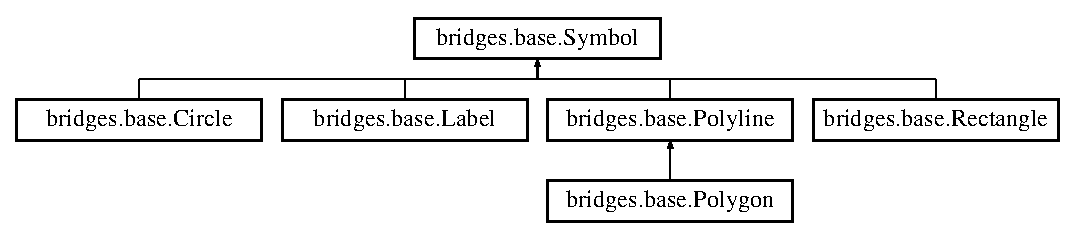
\includegraphics[height=1.942196cm]{classbridges_1_1base_1_1_symbol}
\end{center}
\end{figure}


\subsection{Detailed Description}
This is a class in B\+R\+I\+D\+G\+ES for deriving a number of \hyperlink{classbridges_1_1base_1_1_symbol}{Symbol} objects for use in a \hyperlink{classbridges_1_1base_1_1_symbol_collection}{Symbol\+Collection}. 

It is not intended that objects from this class will be directly created. Rather, we expect that classes that derive from this class be instantiated such as \hyperlink{classbridges_1_1base_1_1_circle}{Circle}, \hyperlink{classbridges_1_1base_1_1_polyline}{Polyline}, \hyperlink{classbridges_1_1base_1_1_polygon}{Polygon}, \hyperlink{classbridges_1_1base_1_1_rectangle}{Rectangle}, \hyperlink{classbridges_1_1base_1_1_text}{Text}.

Symbols correspond to a simplified subset of S\+VG paths and shapes for custom visual representations in B\+R\+I\+D\+G\+ES.

The stroke is the actual lines that get drawn (such as the perimeter of a rectangle) and its style is controlled by \hyperlink{classbridges_1_1base_1_1_symbol_a10abfbf4651ffdc630121da84e23b116}{set\+Stroke\+Color()}, \hyperlink{classbridges_1_1base_1_1_symbol_a4b1ce1fdbc8e76538e67a292e150083c}{set\+Stroke\+Width()}, and \hyperlink{classbridges_1_1base_1_1_symbol_ad36224ec7cb588dbbaa8040ef59ffbfc}{set\+Stroke\+Dash()}.

The inside of the \hyperlink{classbridges_1_1base_1_1_symbol}{Symbol} can be colored independently from the stroke using \hyperlink{classbridges_1_1base_1_1_symbol_a5d3faeffe2dbff7207a4f3d663a34763}{set\+Fill\+Color()}.

Affine transformations are supported with each symbol. If specified, these will transform the shape (pre-\/multiply); translation, rotation and scale transforms are supported. These can be chained to form a composite transform

The overall \hyperlink{classbridges_1_1base_1_1_symbol}{Symbol} can be made more of less visible by adjusting its opacity using \hyperlink{classbridges_1_1base_1_1_symbol_abac237b439448cbef3744817d14061c5}{set\+Opacity()}. \begin{DoxyVerb}@author David Burlinson, Kalpathi Subramanian, Erik Saule
\end{DoxyVerb}


\begin{DoxyDate}{Date}
2018, 7/15/19 

2020, 6/22/21 
\end{DoxyDate}
\subsection*{Public Member Functions}
\begin{DoxyCompactItemize}
\item 
\hyperlink{classbridges_1_1base_1_1_symbol_a5449cffb7ffdbab093a110957158acc6}{Symbol} ()
\item 
\hyperlink{classbridges_1_1base_1_1_symbol}{Symbol} \hyperlink{classbridges_1_1base_1_1_symbol_a8b5aa729cfe2cc5baecf6ec0aa29ac34}{set\+Label} (String \hyperlink{classbridges_1_1base_1_1_symbol_ad2adcc82e6a96c2f3c465702502655e9}{label})
\item 
String \hyperlink{classbridges_1_1base_1_1_symbol_a7616c25b288a6e464f4f0b5fe4bd2826}{get\+Label} ()
\item 
\hyperlink{classbridges_1_1base_1_1_symbol}{Symbol} \hyperlink{classbridges_1_1base_1_1_symbol_a5d3faeffe2dbff7207a4f3d663a34763}{set\+Fill\+Color} (String c)
\item 
\hyperlink{classbridges_1_1base_1_1_color}{Color} \hyperlink{classbridges_1_1base_1_1_symbol_aed2e531266c8a3bc563709c6486380cc}{get\+Fill\+Color} ()
\item 
\hyperlink{classbridges_1_1base_1_1_symbol}{Symbol} \hyperlink{classbridges_1_1base_1_1_symbol_a10abfbf4651ffdc630121da84e23b116}{set\+Stroke\+Color} (\hyperlink{classbridges_1_1base_1_1_color}{Color} c)
\item 
\hyperlink{classbridges_1_1base_1_1_symbol}{Symbol} \hyperlink{classbridges_1_1base_1_1_symbol_ae9aa7d4e9b497875017a9b6e0eaab181}{set\+Stroke\+Color} (String c)
\item 
\hyperlink{classbridges_1_1base_1_1_color}{Color} \hyperlink{classbridges_1_1base_1_1_symbol_abd38aaea2fc344adcc8096ed6eb8681c}{get\+Stroke\+Color} ()
\item 
\hyperlink{classbridges_1_1base_1_1_symbol}{Symbol} \hyperlink{classbridges_1_1base_1_1_symbol_a4b1ce1fdbc8e76538e67a292e150083c}{set\+Stroke\+Width} (float strokewidth)
\begin{DoxyCompactList}\small\item\em This method sets the symbol stroke width. \end{DoxyCompactList}\item 
Float \hyperlink{classbridges_1_1base_1_1_symbol_aa9f4b8ed61cfd3a30dc979d53526ab4e}{get\+Stroke\+Width} ()
\item 
\hyperlink{classbridges_1_1base_1_1_symbol}{Symbol} \hyperlink{classbridges_1_1base_1_1_symbol_abac237b439448cbef3744817d14061c5}{set\+Opacity} (float op)
\begin{DoxyCompactList}\small\item\em This method sets the symbol opacity. \end{DoxyCompactList}\item 
Float \hyperlink{classbridges_1_1base_1_1_symbol_a0135a9633599ee1a463f7bd83c425d02}{get\+Opacity} ()
\item 
\hyperlink{classbridges_1_1base_1_1_symbol}{Symbol} \hyperlink{classbridges_1_1base_1_1_symbol_ad36224ec7cb588dbbaa8040ef59ffbfc}{set\+Stroke\+Dash} (int dash)
\item 
Integer \hyperlink{classbridges_1_1base_1_1_symbol_a31ff460ae6b24ed968c1045e2533a967}{get\+Stroke\+Dash} ()
\item 
\hyperlink{classbridges_1_1base_1_1_symbol}{Symbol} \hyperlink{classbridges_1_1base_1_1_symbol_ad3379aae13939c3cb8aa8b3144ea9bac}{set\+Layer} (int \hyperlink{classbridges_1_1base_1_1_symbol_ad717768b1cd7510be1f4b9049fd04c1f}{layer})
\item 
Integer \hyperlink{classbridges_1_1base_1_1_symbol_ac5048d3027a5ba930ad66c490b55e2e6}{get\+Layer} ()
\item 
float \mbox{[}$\,$\mbox{]}\mbox{[}$\,$\mbox{]} \hyperlink{classbridges_1_1base_1_1_symbol_a26e22be6446757ba7e05f0519ad0167c}{identity} (float\mbox{[}$\,$\mbox{]}\mbox{[}$\,$\mbox{]} m)
\item 
\hyperlink{classbridges_1_1base_1_1_symbol}{Symbol} \hyperlink{classbridges_1_1base_1_1_symbol_a6313c517510bd2363d5c3e46a34f1312}{translate} (float tx, float ty)
\item 
\hyperlink{classbridges_1_1base_1_1_symbol}{Symbol} \hyperlink{classbridges_1_1base_1_1_symbol_a34c091fbe99b1e16a1648e66eca41253}{scale} (float s)
\item 
\hyperlink{classbridges_1_1base_1_1_symbol}{Symbol} \hyperlink{classbridges_1_1base_1_1_symbol_ac0b434638e271e80eca52ca0306f64bf}{scale} (float sx, float sy)
\item 
\hyperlink{classbridges_1_1base_1_1_symbol}{Symbol} \hyperlink{classbridges_1_1base_1_1_symbol_a1104bb7acb941b8fa7325eec8fec0017}{rotate} (float angle)
\item 
\hyperlink{classbridges_1_1base_1_1_symbol}{Symbol} \hyperlink{classbridges_1_1base_1_1_symbol_a39c23fde67b1cfce4ef09b84c5a4b10e}{scale} (float sx, float sy, float px, float py)
\item 
\hyperlink{classbridges_1_1base_1_1_symbol}{Symbol} \hyperlink{classbridges_1_1base_1_1_symbol_a641536133905ee0141d87ba928cdc451}{rotate} (float angle, float px, float py)
\item 
\hyperlink{classbridges_1_1base_1_1_symbol}{Symbol} \hyperlink{classbridges_1_1base_1_1_symbol_ac279dbc8b1e22e3aa64c8b529dbc46d2}{set\+Transform} (float a, float b, float c, float d, float e, float f)
\item 
float \mbox{[}$\,$\mbox{]}\mbox{[}$\,$\mbox{]} \hyperlink{classbridges_1_1base_1_1_symbol_a1660fd3420a9d16a0248bc56a459782e}{get\+Transform} ()
\item 
J\+S\+O\+N\+Object \hyperlink{classbridges_1_1base_1_1_symbol_aeba4cfa5b39fe03e72a568a8b7452e60}{get\+J\+S\+O\+N\+Representation} ()
\item 
void \hyperlink{classbridges_1_1base_1_1_symbol_ad27f1041dad61e288bba42e3c1cf4d52}{add\+All\+J\+S\+ON} (J\+S\+O\+N\+Array symbol\+\_\+json, Integer parent)
\end{DoxyCompactItemize}
\subsection*{Protected Member Functions}
\begin{DoxyCompactItemize}
\item 
String \hyperlink{classbridges_1_1base_1_1_symbol_a10f3cde5331f1af9303b08249e719a9d}{get\+Shape\+Type} ()
\end{DoxyCompactItemize}
\subsection*{Protected Attributes}
\begin{DoxyCompactItemize}
\item 
String \hyperlink{classbridges_1_1base_1_1_symbol_ad2adcc82e6a96c2f3c465702502655e9}{label} = null
\item 
\hyperlink{classbridges_1_1base_1_1_color}{Color} \hyperlink{classbridges_1_1base_1_1_symbol_a44f00712b6c584c7778ed9de4c394cbf}{fill\+Color} = null
\item 
Float \hyperlink{classbridges_1_1base_1_1_symbol_a7a01e5219d556a24e923885fe1646abb}{opacity} = null
\item 
\hyperlink{classbridges_1_1base_1_1_color}{Color} \hyperlink{classbridges_1_1base_1_1_symbol_a51a9a36983b00156284d86ca80cccfb0}{stroke\+Color} = null
\item 
Float \hyperlink{classbridges_1_1base_1_1_symbol_a9f90a6efb9cb7a2f4e38c46862ae5a95}{stroke\+Width} = null
\item 
Integer \hyperlink{classbridges_1_1base_1_1_symbol_a04134e835474c4747e334389f00513c0}{stroke\+Dash} = null
\item 
Integer \hyperlink{classbridges_1_1base_1_1_symbol_ad717768b1cd7510be1f4b9049fd04c1f}{layer} = null
\item 
float \mbox{[}$\,$\mbox{]} \hyperlink{classbridges_1_1base_1_1_symbol_a699a3e8ab079cb166e39d7edeeb8b174}{transform} = null
\end{DoxyCompactItemize}


\subsection{Constructor \& Destructor Documentation}
\mbox{\Hypertarget{classbridges_1_1base_1_1_symbol_a5449cffb7ffdbab093a110957158acc6}\label{classbridges_1_1base_1_1_symbol_a5449cffb7ffdbab093a110957158acc6}} 
\index{bridges\+::base\+::\+Symbol@{bridges\+::base\+::\+Symbol}!Symbol@{Symbol}}
\index{Symbol@{Symbol}!bridges\+::base\+::\+Symbol@{bridges\+::base\+::\+Symbol}}
\subsubsection{\texorpdfstring{Symbol()}{Symbol()}}
{\footnotesize\ttfamily bridges.\+base.\+Symbol.\+Symbol (\begin{DoxyParamCaption}{ }\end{DoxyParamCaption})}

Create a default symbol object 

\subsection{Member Function Documentation}
\mbox{\Hypertarget{classbridges_1_1base_1_1_symbol_ad27f1041dad61e288bba42e3c1cf4d52}\label{classbridges_1_1base_1_1_symbol_ad27f1041dad61e288bba42e3c1cf4d52}} 
\index{bridges\+::base\+::\+Symbol@{bridges\+::base\+::\+Symbol}!add\+All\+J\+S\+ON@{add\+All\+J\+S\+ON}}
\index{add\+All\+J\+S\+ON@{add\+All\+J\+S\+ON}!bridges\+::base\+::\+Symbol@{bridges\+::base\+::\+Symbol}}
\subsubsection{\texorpdfstring{add\+All\+J\+S\+O\+N()}{addAllJSON()}}
{\footnotesize\ttfamily void bridges.\+base.\+Symbol.\+add\+All\+J\+S\+ON (\begin{DoxyParamCaption}\item[{J\+S\+O\+N\+Array}]{symbol\+\_\+json,  }\item[{Integer}]{parent }\end{DoxyParamCaption})}

\mbox{\Hypertarget{classbridges_1_1base_1_1_symbol_aed2e531266c8a3bc563709c6486380cc}\label{classbridges_1_1base_1_1_symbol_aed2e531266c8a3bc563709c6486380cc}} 
\index{bridges\+::base\+::\+Symbol@{bridges\+::base\+::\+Symbol}!get\+Fill\+Color@{get\+Fill\+Color}}
\index{get\+Fill\+Color@{get\+Fill\+Color}!bridges\+::base\+::\+Symbol@{bridges\+::base\+::\+Symbol}}
\subsubsection{\texorpdfstring{get\+Fill\+Color()}{getFillColor()}}
{\footnotesize\ttfamily \hyperlink{classbridges_1_1base_1_1_color}{Color} bridges.\+base.\+Symbol.\+get\+Fill\+Color (\begin{DoxyParamCaption}{ }\end{DoxyParamCaption})}

This method gets fill color

\begin{DoxyReturn}{Returns}
fill color 
\end{DoxyReturn}
\mbox{\Hypertarget{classbridges_1_1base_1_1_symbol_aeba4cfa5b39fe03e72a568a8b7452e60}\label{classbridges_1_1base_1_1_symbol_aeba4cfa5b39fe03e72a568a8b7452e60}} 
\index{bridges\+::base\+::\+Symbol@{bridges\+::base\+::\+Symbol}!get\+J\+S\+O\+N\+Representation@{get\+J\+S\+O\+N\+Representation}}
\index{get\+J\+S\+O\+N\+Representation@{get\+J\+S\+O\+N\+Representation}!bridges\+::base\+::\+Symbol@{bridges\+::base\+::\+Symbol}}
\subsubsection{\texorpdfstring{get\+J\+S\+O\+N\+Representation()}{getJSONRepresentation()}}
{\footnotesize\ttfamily J\+S\+O\+N\+Object bridges.\+base.\+Symbol.\+get\+J\+S\+O\+N\+Representation (\begin{DoxyParamCaption}{ }\end{DoxyParamCaption})}

Internal code for getting the representation of the \hyperlink{classbridges_1_1base_1_1_symbol}{Symbol} object.

\begin{DoxyReturn}{Returns}
the encoded J\+S\+ON string 
\end{DoxyReturn}
\mbox{\Hypertarget{classbridges_1_1base_1_1_symbol_a7616c25b288a6e464f4f0b5fe4bd2826}\label{classbridges_1_1base_1_1_symbol_a7616c25b288a6e464f4f0b5fe4bd2826}} 
\index{bridges\+::base\+::\+Symbol@{bridges\+::base\+::\+Symbol}!get\+Label@{get\+Label}}
\index{get\+Label@{get\+Label}!bridges\+::base\+::\+Symbol@{bridges\+::base\+::\+Symbol}}
\subsubsection{\texorpdfstring{get\+Label()}{getLabel()}}
{\footnotesize\ttfamily String bridges.\+base.\+Symbol.\+get\+Label (\begin{DoxyParamCaption}{ }\end{DoxyParamCaption})}

This method gets the symbol label

\begin{DoxyReturn}{Returns}
symbol label 
\end{DoxyReturn}
\mbox{\Hypertarget{classbridges_1_1base_1_1_symbol_ac5048d3027a5ba930ad66c490b55e2e6}\label{classbridges_1_1base_1_1_symbol_ac5048d3027a5ba930ad66c490b55e2e6}} 
\index{bridges\+::base\+::\+Symbol@{bridges\+::base\+::\+Symbol}!get\+Layer@{get\+Layer}}
\index{get\+Layer@{get\+Layer}!bridges\+::base\+::\+Symbol@{bridges\+::base\+::\+Symbol}}
\subsubsection{\texorpdfstring{get\+Layer()}{getLayer()}}
{\footnotesize\ttfamily Integer bridges.\+base.\+Symbol.\+get\+Layer (\begin{DoxyParamCaption}{ }\end{DoxyParamCaption})}

This method gets layer

\begin{DoxyReturn}{Returns}
layer layer (lower value closer to camera) 
\end{DoxyReturn}
\mbox{\Hypertarget{classbridges_1_1base_1_1_symbol_a0135a9633599ee1a463f7bd83c425d02}\label{classbridges_1_1base_1_1_symbol_a0135a9633599ee1a463f7bd83c425d02}} 
\index{bridges\+::base\+::\+Symbol@{bridges\+::base\+::\+Symbol}!get\+Opacity@{get\+Opacity}}
\index{get\+Opacity@{get\+Opacity}!bridges\+::base\+::\+Symbol@{bridges\+::base\+::\+Symbol}}
\subsubsection{\texorpdfstring{get\+Opacity()}{getOpacity()}}
{\footnotesize\ttfamily Float bridges.\+base.\+Symbol.\+get\+Opacity (\begin{DoxyParamCaption}{ }\end{DoxyParamCaption})}

This method gets symbol opacity

\begin{DoxyReturn}{Returns}
symbol opacity 
\end{DoxyReturn}
\mbox{\Hypertarget{classbridges_1_1base_1_1_symbol_a10f3cde5331f1af9303b08249e719a9d}\label{classbridges_1_1base_1_1_symbol_a10f3cde5331f1af9303b08249e719a9d}} 
\index{bridges\+::base\+::\+Symbol@{bridges\+::base\+::\+Symbol}!get\+Shape\+Type@{get\+Shape\+Type}}
\index{get\+Shape\+Type@{get\+Shape\+Type}!bridges\+::base\+::\+Symbol@{bridges\+::base\+::\+Symbol}}
\subsubsection{\texorpdfstring{get\+Shape\+Type()}{getShapeType()}}
{\footnotesize\ttfamily String bridges.\+base.\+Symbol.\+get\+Shape\+Type (\begin{DoxyParamCaption}{ }\end{DoxyParamCaption})\hspace{0.3cm}{\ttfamily [protected]}}

Get the shape type

\begin{DoxyReturn}{Returns}
shape type 
\end{DoxyReturn}
\mbox{\Hypertarget{classbridges_1_1base_1_1_symbol_abd38aaea2fc344adcc8096ed6eb8681c}\label{classbridges_1_1base_1_1_symbol_abd38aaea2fc344adcc8096ed6eb8681c}} 
\index{bridges\+::base\+::\+Symbol@{bridges\+::base\+::\+Symbol}!get\+Stroke\+Color@{get\+Stroke\+Color}}
\index{get\+Stroke\+Color@{get\+Stroke\+Color}!bridges\+::base\+::\+Symbol@{bridges\+::base\+::\+Symbol}}
\subsubsection{\texorpdfstring{get\+Stroke\+Color()}{getStrokeColor()}}
{\footnotesize\ttfamily \hyperlink{classbridges_1_1base_1_1_color}{Color} bridges.\+base.\+Symbol.\+get\+Stroke\+Color (\begin{DoxyParamCaption}{ }\end{DoxyParamCaption})}

This method gets stroke color

\begin{DoxyReturn}{Returns}
stroke color 
\end{DoxyReturn}
\mbox{\Hypertarget{classbridges_1_1base_1_1_symbol_a31ff460ae6b24ed968c1045e2533a967}\label{classbridges_1_1base_1_1_symbol_a31ff460ae6b24ed968c1045e2533a967}} 
\index{bridges\+::base\+::\+Symbol@{bridges\+::base\+::\+Symbol}!get\+Stroke\+Dash@{get\+Stroke\+Dash}}
\index{get\+Stroke\+Dash@{get\+Stroke\+Dash}!bridges\+::base\+::\+Symbol@{bridges\+::base\+::\+Symbol}}
\subsubsection{\texorpdfstring{get\+Stroke\+Dash()}{getStrokeDash()}}
{\footnotesize\ttfamily Integer bridges.\+base.\+Symbol.\+get\+Stroke\+Dash (\begin{DoxyParamCaption}{ }\end{DoxyParamCaption})}

This method gets stroke dash level

\begin{DoxyReturn}{Returns}
stroke dash level 
\end{DoxyReturn}
\mbox{\Hypertarget{classbridges_1_1base_1_1_symbol_aa9f4b8ed61cfd3a30dc979d53526ab4e}\label{classbridges_1_1base_1_1_symbol_aa9f4b8ed61cfd3a30dc979d53526ab4e}} 
\index{bridges\+::base\+::\+Symbol@{bridges\+::base\+::\+Symbol}!get\+Stroke\+Width@{get\+Stroke\+Width}}
\index{get\+Stroke\+Width@{get\+Stroke\+Width}!bridges\+::base\+::\+Symbol@{bridges\+::base\+::\+Symbol}}
\subsubsection{\texorpdfstring{get\+Stroke\+Width()}{getStrokeWidth()}}
{\footnotesize\ttfamily Float bridges.\+base.\+Symbol.\+get\+Stroke\+Width (\begin{DoxyParamCaption}{ }\end{DoxyParamCaption})}

This method gets stroke width

\begin{DoxyReturn}{Returns}
stroke width 
\end{DoxyReturn}
\mbox{\Hypertarget{classbridges_1_1base_1_1_symbol_a1660fd3420a9d16a0248bc56a459782e}\label{classbridges_1_1base_1_1_symbol_a1660fd3420a9d16a0248bc56a459782e}} 
\index{bridges\+::base\+::\+Symbol@{bridges\+::base\+::\+Symbol}!get\+Transform@{get\+Transform}}
\index{get\+Transform@{get\+Transform}!bridges\+::base\+::\+Symbol@{bridges\+::base\+::\+Symbol}}
\subsubsection{\texorpdfstring{get\+Transform()}{getTransform()}}
{\footnotesize\ttfamily float \mbox{[}$\,$\mbox{]}\mbox{[}$\,$\mbox{]} bridges.\+base.\+Symbol.\+get\+Transform (\begin{DoxyParamCaption}{ }\end{DoxyParamCaption})}

This method returns the affine transformation associated with this symbol

\begin{DoxyReturn}{Returns}
transformation matrix 
\end{DoxyReturn}
\mbox{\Hypertarget{classbridges_1_1base_1_1_symbol_a26e22be6446757ba7e05f0519ad0167c}\label{classbridges_1_1base_1_1_symbol_a26e22be6446757ba7e05f0519ad0167c}} 
\index{bridges\+::base\+::\+Symbol@{bridges\+::base\+::\+Symbol}!identity@{identity}}
\index{identity@{identity}!bridges\+::base\+::\+Symbol@{bridges\+::base\+::\+Symbol}}
\subsubsection{\texorpdfstring{identity()}{identity()}}
{\footnotesize\ttfamily float \mbox{[}$\,$\mbox{]}\mbox{[}$\,$\mbox{]} bridges.\+base.\+Symbol.\+identity (\begin{DoxyParamCaption}\item[{float}]{m\mbox{[}$\,$\mbox{]}\mbox{[}$\,$\mbox{]} }\end{DoxyParamCaption})}

create the identity matrix


\begin{DoxyParams}{Parameters}
{\em m} & 3x3 input matrix \\
\hline
\end{DoxyParams}
\mbox{\Hypertarget{classbridges_1_1base_1_1_symbol_a1104bb7acb941b8fa7325eec8fec0017}\label{classbridges_1_1base_1_1_symbol_a1104bb7acb941b8fa7325eec8fec0017}} 
\index{bridges\+::base\+::\+Symbol@{bridges\+::base\+::\+Symbol}!rotate@{rotate}}
\index{rotate@{rotate}!bridges\+::base\+::\+Symbol@{bridges\+::base\+::\+Symbol}}
\subsubsection{\texorpdfstring{rotate()}{rotate()}\hspace{0.1cm}{\footnotesize\ttfamily [1/2]}}
{\footnotesize\ttfamily \hyperlink{classbridges_1_1base_1_1_symbol}{Symbol} bridges.\+base.\+Symbol.\+rotate (\begin{DoxyParamCaption}\item[{float}]{angle }\end{DoxyParamCaption})}

rotate the symbol by angle theta about Z axis (2D rotation), updates the current transform matrix; note\+: rotation is about the origin


\begin{DoxyParams}{Parameters}
{\em angle} & angle (in degrees) \\
\hline
\end{DoxyParams}
\mbox{\Hypertarget{classbridges_1_1base_1_1_symbol_a641536133905ee0141d87ba928cdc451}\label{classbridges_1_1base_1_1_symbol_a641536133905ee0141d87ba928cdc451}} 
\index{bridges\+::base\+::\+Symbol@{bridges\+::base\+::\+Symbol}!rotate@{rotate}}
\index{rotate@{rotate}!bridges\+::base\+::\+Symbol@{bridges\+::base\+::\+Symbol}}
\subsubsection{\texorpdfstring{rotate()}{rotate()}\hspace{0.1cm}{\footnotesize\ttfamily [2/2]}}
{\footnotesize\ttfamily \hyperlink{classbridges_1_1base_1_1_symbol}{Symbol} bridges.\+base.\+Symbol.\+rotate (\begin{DoxyParamCaption}\item[{float}]{angle,  }\item[{float}]{px,  }\item[{float}]{py }\end{DoxyParamCaption})}

rotate the symbol by angle theta about Z axis (2D rotation) about the point (px, py)


\begin{DoxyParams}{Parameters}
{\em angle} & angle (in degrees) \\
\hline
\end{DoxyParams}
\mbox{\Hypertarget{classbridges_1_1base_1_1_symbol_a34c091fbe99b1e16a1648e66eca41253}\label{classbridges_1_1base_1_1_symbol_a34c091fbe99b1e16a1648e66eca41253}} 
\index{bridges\+::base\+::\+Symbol@{bridges\+::base\+::\+Symbol}!scale@{scale}}
\index{scale@{scale}!bridges\+::base\+::\+Symbol@{bridges\+::base\+::\+Symbol}}
\subsubsection{\texorpdfstring{scale()}{scale()}\hspace{0.1cm}{\footnotesize\ttfamily [1/3]}}
{\footnotesize\ttfamily \hyperlink{classbridges_1_1base_1_1_symbol}{Symbol} bridges.\+base.\+Symbol.\+scale (\begin{DoxyParamCaption}\item[{float}]{s }\end{DoxyParamCaption})}

scale the symbol by s along X and Y axes updates the current transform matrix; note\+: scale is about the origin


\begin{DoxyParams}{Parameters}
{\em s} & scale factor \\
\hline
\end{DoxyParams}
\mbox{\Hypertarget{classbridges_1_1base_1_1_symbol_ac0b434638e271e80eca52ca0306f64bf}\label{classbridges_1_1base_1_1_symbol_ac0b434638e271e80eca52ca0306f64bf}} 
\index{bridges\+::base\+::\+Symbol@{bridges\+::base\+::\+Symbol}!scale@{scale}}
\index{scale@{scale}!bridges\+::base\+::\+Symbol@{bridges\+::base\+::\+Symbol}}
\subsubsection{\texorpdfstring{scale()}{scale()}\hspace{0.1cm}{\footnotesize\ttfamily [2/3]}}
{\footnotesize\ttfamily \hyperlink{classbridges_1_1base_1_1_symbol}{Symbol} bridges.\+base.\+Symbol.\+scale (\begin{DoxyParamCaption}\item[{float}]{sx,  }\item[{float}]{sy }\end{DoxyParamCaption})}

scale the symbol by sx, sy along the X and Y axes, updates the current transform matrix; note\+: scale is about the origin


\begin{DoxyParams}{Parameters}
{\em sx} & scale factor in X \\
\hline
{\em sy} & scale factor in Y \\
\hline
\end{DoxyParams}
\mbox{\Hypertarget{classbridges_1_1base_1_1_symbol_a39c23fde67b1cfce4ef09b84c5a4b10e}\label{classbridges_1_1base_1_1_symbol_a39c23fde67b1cfce4ef09b84c5a4b10e}} 
\index{bridges\+::base\+::\+Symbol@{bridges\+::base\+::\+Symbol}!scale@{scale}}
\index{scale@{scale}!bridges\+::base\+::\+Symbol@{bridges\+::base\+::\+Symbol}}
\subsubsection{\texorpdfstring{scale()}{scale()}\hspace{0.1cm}{\footnotesize\ttfamily [3/3]}}
{\footnotesize\ttfamily \hyperlink{classbridges_1_1base_1_1_symbol}{Symbol} bridges.\+base.\+Symbol.\+scale (\begin{DoxyParamCaption}\item[{float}]{sx,  }\item[{float}]{sy,  }\item[{float}]{px,  }\item[{float}]{py }\end{DoxyParamCaption})}

scale the symbol by (sx, sy) along the X and Y axes about the point (px, py); updates the current transform matrix;


\begin{DoxyParams}{Parameters}
{\em sx} & scale factor in X \\
\hline
{\em sy} & scale factor in Y \\
\hline
{\em px} & x coordinate of point \\
\hline
{\em py} & y coordinate of point \\
\hline
\end{DoxyParams}
\mbox{\Hypertarget{classbridges_1_1base_1_1_symbol_a5d3faeffe2dbff7207a4f3d663a34763}\label{classbridges_1_1base_1_1_symbol_a5d3faeffe2dbff7207a4f3d663a34763}} 
\index{bridges\+::base\+::\+Symbol@{bridges\+::base\+::\+Symbol}!set\+Fill\+Color@{set\+Fill\+Color}}
\index{set\+Fill\+Color@{set\+Fill\+Color}!bridges\+::base\+::\+Symbol@{bridges\+::base\+::\+Symbol}}
\subsubsection{\texorpdfstring{set\+Fill\+Color()}{setFillColor()}}
{\footnotesize\ttfamily \hyperlink{classbridges_1_1base_1_1_symbol}{Symbol} bridges.\+base.\+Symbol.\+set\+Fill\+Color (\begin{DoxyParamCaption}\item[{String}]{c }\end{DoxyParamCaption})}

This method sets the symbol fill color


\begin{DoxyParams}{Parameters}
{\em c} & the color to set \\
\hline
\end{DoxyParams}
\begin{DoxyReturn}{Returns}
the symbol 
\end{DoxyReturn}
\mbox{\Hypertarget{classbridges_1_1base_1_1_symbol_a8b5aa729cfe2cc5baecf6ec0aa29ac34}\label{classbridges_1_1base_1_1_symbol_a8b5aa729cfe2cc5baecf6ec0aa29ac34}} 
\index{bridges\+::base\+::\+Symbol@{bridges\+::base\+::\+Symbol}!set\+Label@{set\+Label}}
\index{set\+Label@{set\+Label}!bridges\+::base\+::\+Symbol@{bridges\+::base\+::\+Symbol}}
\subsubsection{\texorpdfstring{set\+Label()}{setLabel()}}
{\footnotesize\ttfamily \hyperlink{classbridges_1_1base_1_1_symbol}{Symbol} bridges.\+base.\+Symbol.\+set\+Label (\begin{DoxyParamCaption}\item[{String}]{label }\end{DoxyParamCaption})}

This method sets the label


\begin{DoxyParams}{Parameters}
{\em label} & the label to set \\
\hline
\end{DoxyParams}
\mbox{\Hypertarget{classbridges_1_1base_1_1_symbol_ad3379aae13939c3cb8aa8b3144ea9bac}\label{classbridges_1_1base_1_1_symbol_ad3379aae13939c3cb8aa8b3144ea9bac}} 
\index{bridges\+::base\+::\+Symbol@{bridges\+::base\+::\+Symbol}!set\+Layer@{set\+Layer}}
\index{set\+Layer@{set\+Layer}!bridges\+::base\+::\+Symbol@{bridges\+::base\+::\+Symbol}}
\subsubsection{\texorpdfstring{set\+Layer()}{setLayer()}}
{\footnotesize\ttfamily \hyperlink{classbridges_1_1base_1_1_symbol}{Symbol} bridges.\+base.\+Symbol.\+set\+Layer (\begin{DoxyParamCaption}\item[{int}]{layer }\end{DoxyParamCaption})}

This method sets the layer the symbol sits on


\begin{DoxyParams}{Parameters}
{\em layer} & layer (lower value closer to camera) \\
\hline
\end{DoxyParams}
\begin{DoxyReturn}{Returns}
the symbol 
\end{DoxyReturn}
\mbox{\Hypertarget{classbridges_1_1base_1_1_symbol_abac237b439448cbef3744817d14061c5}\label{classbridges_1_1base_1_1_symbol_abac237b439448cbef3744817d14061c5}} 
\index{bridges\+::base\+::\+Symbol@{bridges\+::base\+::\+Symbol}!set\+Opacity@{set\+Opacity}}
\index{set\+Opacity@{set\+Opacity}!bridges\+::base\+::\+Symbol@{bridges\+::base\+::\+Symbol}}
\subsubsection{\texorpdfstring{set\+Opacity()}{setOpacity()}}
{\footnotesize\ttfamily \hyperlink{classbridges_1_1base_1_1_symbol}{Symbol} bridges.\+base.\+Symbol.\+set\+Opacity (\begin{DoxyParamCaption}\item[{float}]{op }\end{DoxyParamCaption})}



This method sets the symbol opacity. 


\begin{DoxyParams}{Parameters}
{\em op} & the opacity to set \\
\hline
\end{DoxyParams}
\begin{DoxyReturn}{Returns}
the symbol 
\end{DoxyReturn}
\mbox{\Hypertarget{classbridges_1_1base_1_1_symbol_a10abfbf4651ffdc630121da84e23b116}\label{classbridges_1_1base_1_1_symbol_a10abfbf4651ffdc630121da84e23b116}} 
\index{bridges\+::base\+::\+Symbol@{bridges\+::base\+::\+Symbol}!set\+Stroke\+Color@{set\+Stroke\+Color}}
\index{set\+Stroke\+Color@{set\+Stroke\+Color}!bridges\+::base\+::\+Symbol@{bridges\+::base\+::\+Symbol}}
\subsubsection{\texorpdfstring{set\+Stroke\+Color()}{setStrokeColor()}\hspace{0.1cm}{\footnotesize\ttfamily [1/2]}}
{\footnotesize\ttfamily \hyperlink{classbridges_1_1base_1_1_symbol}{Symbol} bridges.\+base.\+Symbol.\+set\+Stroke\+Color (\begin{DoxyParamCaption}\item[{\hyperlink{classbridges_1_1base_1_1_color}{Color}}]{c }\end{DoxyParamCaption})}

This method sets the symbol stroke color


\begin{DoxyParams}{Parameters}
{\em c} & the color to set \\
\hline
\end{DoxyParams}
\begin{DoxyReturn}{Returns}
the symbol 
\end{DoxyReturn}
\mbox{\Hypertarget{classbridges_1_1base_1_1_symbol_ae9aa7d4e9b497875017a9b6e0eaab181}\label{classbridges_1_1base_1_1_symbol_ae9aa7d4e9b497875017a9b6e0eaab181}} 
\index{bridges\+::base\+::\+Symbol@{bridges\+::base\+::\+Symbol}!set\+Stroke\+Color@{set\+Stroke\+Color}}
\index{set\+Stroke\+Color@{set\+Stroke\+Color}!bridges\+::base\+::\+Symbol@{bridges\+::base\+::\+Symbol}}
\subsubsection{\texorpdfstring{set\+Stroke\+Color()}{setStrokeColor()}\hspace{0.1cm}{\footnotesize\ttfamily [2/2]}}
{\footnotesize\ttfamily \hyperlink{classbridges_1_1base_1_1_symbol}{Symbol} bridges.\+base.\+Symbol.\+set\+Stroke\+Color (\begin{DoxyParamCaption}\item[{String}]{c }\end{DoxyParamCaption})}

This method sets the symbol stroke color


\begin{DoxyParams}{Parameters}
{\em c} & the named color to set \\
\hline
\end{DoxyParams}
\begin{DoxyReturn}{Returns}
the symbol 
\end{DoxyReturn}
\mbox{\Hypertarget{classbridges_1_1base_1_1_symbol_ad36224ec7cb588dbbaa8040ef59ffbfc}\label{classbridges_1_1base_1_1_symbol_ad36224ec7cb588dbbaa8040ef59ffbfc}} 
\index{bridges\+::base\+::\+Symbol@{bridges\+::base\+::\+Symbol}!set\+Stroke\+Dash@{set\+Stroke\+Dash}}
\index{set\+Stroke\+Dash@{set\+Stroke\+Dash}!bridges\+::base\+::\+Symbol@{bridges\+::base\+::\+Symbol}}
\subsubsection{\texorpdfstring{set\+Stroke\+Dash()}{setStrokeDash()}}
{\footnotesize\ttfamily \hyperlink{classbridges_1_1base_1_1_symbol}{Symbol} bridges.\+base.\+Symbol.\+set\+Stroke\+Dash (\begin{DoxyParamCaption}\item[{int}]{dash }\end{DoxyParamCaption})}

This method sets the stroke dash level


\begin{DoxyParams}{Parameters}
{\em dash} & dash level \\
\hline
\end{DoxyParams}
\begin{DoxyReturn}{Returns}
the symbol 
\end{DoxyReturn}
\mbox{\Hypertarget{classbridges_1_1base_1_1_symbol_a4b1ce1fdbc8e76538e67a292e150083c}\label{classbridges_1_1base_1_1_symbol_a4b1ce1fdbc8e76538e67a292e150083c}} 
\index{bridges\+::base\+::\+Symbol@{bridges\+::base\+::\+Symbol}!set\+Stroke\+Width@{set\+Stroke\+Width}}
\index{set\+Stroke\+Width@{set\+Stroke\+Width}!bridges\+::base\+::\+Symbol@{bridges\+::base\+::\+Symbol}}
\subsubsection{\texorpdfstring{set\+Stroke\+Width()}{setStrokeWidth()}}
{\footnotesize\ttfamily \hyperlink{classbridges_1_1base_1_1_symbol}{Symbol} bridges.\+base.\+Symbol.\+set\+Stroke\+Width (\begin{DoxyParamCaption}\item[{float}]{strokewidth }\end{DoxyParamCaption})}



This method sets the symbol stroke width. 

This is the weight of the individual lines that are drawn, such as the perimeter of a rectangle.


\begin{DoxyParams}{Parameters}
{\em strokewidth} & the stroke width to set \\
\hline
\end{DoxyParams}
\begin{DoxyReturn}{Returns}
the symbol 
\end{DoxyReturn}
\mbox{\Hypertarget{classbridges_1_1base_1_1_symbol_ac279dbc8b1e22e3aa64c8b529dbc46d2}\label{classbridges_1_1base_1_1_symbol_ac279dbc8b1e22e3aa64c8b529dbc46d2}} 
\index{bridges\+::base\+::\+Symbol@{bridges\+::base\+::\+Symbol}!set\+Transform@{set\+Transform}}
\index{set\+Transform@{set\+Transform}!bridges\+::base\+::\+Symbol@{bridges\+::base\+::\+Symbol}}
\subsubsection{\texorpdfstring{set\+Transform()}{setTransform()}}
{\footnotesize\ttfamily \hyperlink{classbridges_1_1base_1_1_symbol}{Symbol} bridges.\+base.\+Symbol.\+set\+Transform (\begin{DoxyParamCaption}\item[{float}]{a,  }\item[{float}]{b,  }\item[{float}]{c,  }\item[{float}]{d,  }\item[{float}]{e,  }\item[{float}]{f }\end{DoxyParamCaption})}

This method sets the transform matrix for this symbol; terms passed in column major order.


\begin{DoxyParams}{Parameters}
{\em a} & transformation term \\
\hline
{\em b} & transformation term \\
\hline
{\em c} & transformation term \\
\hline
{\em d} & transformation term \\
\hline
{\em e} & transformation term \\
\hline
{\em f} & transformation term\\
\hline
\end{DoxyParams}
\begin{DoxyReturn}{Returns}
the symbol 
\end{DoxyReturn}
\mbox{\Hypertarget{classbridges_1_1base_1_1_symbol_a6313c517510bd2363d5c3e46a34f1312}\label{classbridges_1_1base_1_1_symbol_a6313c517510bd2363d5c3e46a34f1312}} 
\index{bridges\+::base\+::\+Symbol@{bridges\+::base\+::\+Symbol}!translate@{translate}}
\index{translate@{translate}!bridges\+::base\+::\+Symbol@{bridges\+::base\+::\+Symbol}}
\subsubsection{\texorpdfstring{translate()}{translate()}}
{\footnotesize\ttfamily \hyperlink{classbridges_1_1base_1_1_symbol}{Symbol} bridges.\+base.\+Symbol.\+translate (\begin{DoxyParamCaption}\item[{float}]{tx,  }\item[{float}]{ty }\end{DoxyParamCaption})}

translate the symbol by tx, ty along the X and Y axes, updates the current transform matrix


\begin{DoxyParams}{Parameters}
{\em tx} & translation in X \\
\hline
{\em ty} & translation in Y \\
\hline
\end{DoxyParams}


\subsection{Member Data Documentation}
\mbox{\Hypertarget{classbridges_1_1base_1_1_symbol_a44f00712b6c584c7778ed9de4c394cbf}\label{classbridges_1_1base_1_1_symbol_a44f00712b6c584c7778ed9de4c394cbf}} 
\index{bridges\+::base\+::\+Symbol@{bridges\+::base\+::\+Symbol}!fill\+Color@{fill\+Color}}
\index{fill\+Color@{fill\+Color}!bridges\+::base\+::\+Symbol@{bridges\+::base\+::\+Symbol}}
\subsubsection{\texorpdfstring{fill\+Color}{fillColor}}
{\footnotesize\ttfamily \hyperlink{classbridges_1_1base_1_1_color}{Color} bridges.\+base.\+Symbol.\+fill\+Color = null\hspace{0.3cm}{\ttfamily [protected]}}

\mbox{\Hypertarget{classbridges_1_1base_1_1_symbol_ad2adcc82e6a96c2f3c465702502655e9}\label{classbridges_1_1base_1_1_symbol_ad2adcc82e6a96c2f3c465702502655e9}} 
\index{bridges\+::base\+::\+Symbol@{bridges\+::base\+::\+Symbol}!label@{label}}
\index{label@{label}!bridges\+::base\+::\+Symbol@{bridges\+::base\+::\+Symbol}}
\subsubsection{\texorpdfstring{label}{label}}
{\footnotesize\ttfamily String bridges.\+base.\+Symbol.\+label = null\hspace{0.3cm}{\ttfamily [protected]}}

\mbox{\Hypertarget{classbridges_1_1base_1_1_symbol_ad717768b1cd7510be1f4b9049fd04c1f}\label{classbridges_1_1base_1_1_symbol_ad717768b1cd7510be1f4b9049fd04c1f}} 
\index{bridges\+::base\+::\+Symbol@{bridges\+::base\+::\+Symbol}!layer@{layer}}
\index{layer@{layer}!bridges\+::base\+::\+Symbol@{bridges\+::base\+::\+Symbol}}
\subsubsection{\texorpdfstring{layer}{layer}}
{\footnotesize\ttfamily Integer bridges.\+base.\+Symbol.\+layer = null\hspace{0.3cm}{\ttfamily [protected]}}

\mbox{\Hypertarget{classbridges_1_1base_1_1_symbol_a7a01e5219d556a24e923885fe1646abb}\label{classbridges_1_1base_1_1_symbol_a7a01e5219d556a24e923885fe1646abb}} 
\index{bridges\+::base\+::\+Symbol@{bridges\+::base\+::\+Symbol}!opacity@{opacity}}
\index{opacity@{opacity}!bridges\+::base\+::\+Symbol@{bridges\+::base\+::\+Symbol}}
\subsubsection{\texorpdfstring{opacity}{opacity}}
{\footnotesize\ttfamily Float bridges.\+base.\+Symbol.\+opacity = null\hspace{0.3cm}{\ttfamily [protected]}}

\mbox{\Hypertarget{classbridges_1_1base_1_1_symbol_a51a9a36983b00156284d86ca80cccfb0}\label{classbridges_1_1base_1_1_symbol_a51a9a36983b00156284d86ca80cccfb0}} 
\index{bridges\+::base\+::\+Symbol@{bridges\+::base\+::\+Symbol}!stroke\+Color@{stroke\+Color}}
\index{stroke\+Color@{stroke\+Color}!bridges\+::base\+::\+Symbol@{bridges\+::base\+::\+Symbol}}
\subsubsection{\texorpdfstring{stroke\+Color}{strokeColor}}
{\footnotesize\ttfamily \hyperlink{classbridges_1_1base_1_1_color}{Color} bridges.\+base.\+Symbol.\+stroke\+Color = null\hspace{0.3cm}{\ttfamily [protected]}}

\mbox{\Hypertarget{classbridges_1_1base_1_1_symbol_a04134e835474c4747e334389f00513c0}\label{classbridges_1_1base_1_1_symbol_a04134e835474c4747e334389f00513c0}} 
\index{bridges\+::base\+::\+Symbol@{bridges\+::base\+::\+Symbol}!stroke\+Dash@{stroke\+Dash}}
\index{stroke\+Dash@{stroke\+Dash}!bridges\+::base\+::\+Symbol@{bridges\+::base\+::\+Symbol}}
\subsubsection{\texorpdfstring{stroke\+Dash}{strokeDash}}
{\footnotesize\ttfamily Integer bridges.\+base.\+Symbol.\+stroke\+Dash = null\hspace{0.3cm}{\ttfamily [protected]}}

\mbox{\Hypertarget{classbridges_1_1base_1_1_symbol_a9f90a6efb9cb7a2f4e38c46862ae5a95}\label{classbridges_1_1base_1_1_symbol_a9f90a6efb9cb7a2f4e38c46862ae5a95}} 
\index{bridges\+::base\+::\+Symbol@{bridges\+::base\+::\+Symbol}!stroke\+Width@{stroke\+Width}}
\index{stroke\+Width@{stroke\+Width}!bridges\+::base\+::\+Symbol@{bridges\+::base\+::\+Symbol}}
\subsubsection{\texorpdfstring{stroke\+Width}{strokeWidth}}
{\footnotesize\ttfamily Float bridges.\+base.\+Symbol.\+stroke\+Width = null\hspace{0.3cm}{\ttfamily [protected]}}

\mbox{\Hypertarget{classbridges_1_1base_1_1_symbol_a699a3e8ab079cb166e39d7edeeb8b174}\label{classbridges_1_1base_1_1_symbol_a699a3e8ab079cb166e39d7edeeb8b174}} 
\index{bridges\+::base\+::\+Symbol@{bridges\+::base\+::\+Symbol}!transform@{transform}}
\index{transform@{transform}!bridges\+::base\+::\+Symbol@{bridges\+::base\+::\+Symbol}}
\subsubsection{\texorpdfstring{transform}{transform}}
{\footnotesize\ttfamily float \mbox{[}$\,$\mbox{]} bridges.\+base.\+Symbol.\+transform = null\hspace{0.3cm}{\ttfamily [protected]}}



The documentation for this class was generated from the following file\+:\begin{DoxyCompactItemize}
\item 
/home/erik/work/bridges/bridges-\/java/src/main/java/bridges/base/\hyperlink{_symbol_8java}{Symbol.\+java}\end{DoxyCompactItemize}

\hypertarget{classbridges_1_1base_1_1_symbol_collection}{}\section{bridges.\+base.\+Symbol\+Collection Class Reference}
\label{classbridges_1_1base_1_1_symbol_collection}\index{bridges.\+base.\+Symbol\+Collection@{bridges.\+base.\+Symbol\+Collection}}
Inheritance diagram for bridges.\+base.\+Symbol\+Collection\+:\begin{figure}[H]
\begin{center}
\leavevmode
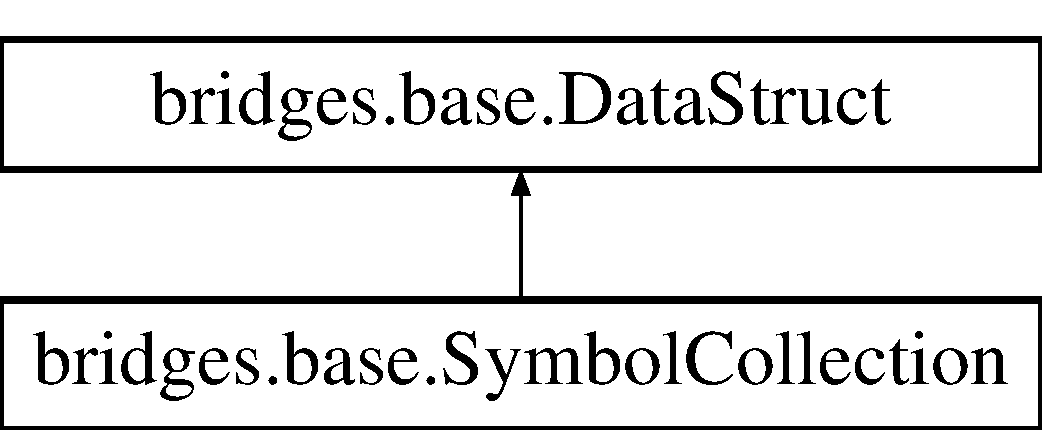
\includegraphics[height=2.000000cm]{classbridges_1_1base_1_1_symbol_collection}
\end{center}
\end{figure}
\subsection*{Public Member Functions}
\begin{DoxyCompactItemize}
\item 
\hyperlink{classbridges_1_1base_1_1_symbol_collection_a8959dab963ce54f56560c6c27a3a3de5}{Symbol\+Collection} ()
\item 
String \hyperlink{classbridges_1_1base_1_1_symbol_collection_afbc928d2e6818edec96d10f52feebacb}{get\+Data\+Struct\+Type} ()
\item 
void \hyperlink{classbridges_1_1base_1_1_symbol_collection_a8e934c53b78b05a7e982f3ff2362adea}{add\+Symbol} (\hyperlink{classbridges_1_1base_1_1_symbol}{Symbol} s)
\item 
String \hyperlink{classbridges_1_1base_1_1_symbol_collection_a706ad8a7bcf12c194403ac3281c73674}{get\+Data\+Structure\+Representation} ()
\end{DoxyCompactItemize}
\subsection*{Protected Attributes}
\begin{DoxyCompactItemize}
\item 
Float \hyperlink{classbridges_1_1base_1_1_symbol_collection_a7624e96d2a4b5b6264791eb8dacbd350}{domain} = 100.\+0f
\end{DoxyCompactItemize}


\subsection{Constructor \& Destructor Documentation}
\hypertarget{classbridges_1_1base_1_1_symbol_collection_a8959dab963ce54f56560c6c27a3a3de5}{}\index{bridges\+::base\+::\+Symbol\+Collection@{bridges\+::base\+::\+Symbol\+Collection}!Symbol\+Collection@{Symbol\+Collection}}
\index{Symbol\+Collection@{Symbol\+Collection}!bridges\+::base\+::\+Symbol\+Collection@{bridges\+::base\+::\+Symbol\+Collection}}
\subsubsection[{Symbol\+Collection()}]{\setlength{\rightskip}{0pt plus 5cm}bridges.\+base.\+Symbol\+Collection.\+Symbol\+Collection (
\begin{DoxyParamCaption}
{}
\end{DoxyParamCaption}
)}\label{classbridges_1_1base_1_1_symbol_collection_a8959dab963ce54f56560c6c27a3a3de5}
Constructor 

\subsection{Member Function Documentation}
\hypertarget{classbridges_1_1base_1_1_symbol_collection_a8e934c53b78b05a7e982f3ff2362adea}{}\index{bridges\+::base\+::\+Symbol\+Collection@{bridges\+::base\+::\+Symbol\+Collection}!add\+Symbol@{add\+Symbol}}
\index{add\+Symbol@{add\+Symbol}!bridges\+::base\+::\+Symbol\+Collection@{bridges\+::base\+::\+Symbol\+Collection}}
\subsubsection[{add\+Symbol(\+Symbol s)}]{\setlength{\rightskip}{0pt plus 5cm}void bridges.\+base.\+Symbol\+Collection.\+add\+Symbol (
\begin{DoxyParamCaption}
\item[{{\bf Symbol}}]{s}
\end{DoxyParamCaption}
)}\label{classbridges_1_1base_1_1_symbol_collection_a8e934c53b78b05a7e982f3ff2362adea}
This method adds a symbol to the collection \hypertarget{classbridges_1_1base_1_1_symbol_collection_afbc928d2e6818edec96d10f52feebacb}{}\index{bridges\+::base\+::\+Symbol\+Collection@{bridges\+::base\+::\+Symbol\+Collection}!get\+Data\+Struct\+Type@{get\+Data\+Struct\+Type}}
\index{get\+Data\+Struct\+Type@{get\+Data\+Struct\+Type}!bridges\+::base\+::\+Symbol\+Collection@{bridges\+::base\+::\+Symbol\+Collection}}
\subsubsection[{get\+Data\+Struct\+Type()}]{\setlength{\rightskip}{0pt plus 5cm}String bridges.\+base.\+Symbol\+Collection.\+get\+Data\+Struct\+Type (
\begin{DoxyParamCaption}
{}
\end{DoxyParamCaption}
)}\label{classbridges_1_1base_1_1_symbol_collection_afbc928d2e6818edec96d10f52feebacb}
This method gets the data structure type

\begin{DoxyReturn}{Returns}
The date structure type as a string 
\end{DoxyReturn}
\hypertarget{classbridges_1_1base_1_1_symbol_collection_a706ad8a7bcf12c194403ac3281c73674}{}\index{bridges\+::base\+::\+Symbol\+Collection@{bridges\+::base\+::\+Symbol\+Collection}!get\+Data\+Structure\+Representation@{get\+Data\+Structure\+Representation}}
\index{get\+Data\+Structure\+Representation@{get\+Data\+Structure\+Representation}!bridges\+::base\+::\+Symbol\+Collection@{bridges\+::base\+::\+Symbol\+Collection}}
\subsubsection[{get\+Data\+Structure\+Representation()}]{\setlength{\rightskip}{0pt plus 5cm}String bridges.\+base.\+Symbol\+Collection.\+get\+Data\+Structure\+Representation (
\begin{DoxyParamCaption}
{}
\end{DoxyParamCaption}
)}\label{classbridges_1_1base_1_1_symbol_collection_a706ad8a7bcf12c194403ac3281c73674}


\subsection{Member Data Documentation}
\hypertarget{classbridges_1_1base_1_1_symbol_collection_a7624e96d2a4b5b6264791eb8dacbd350}{}\index{bridges\+::base\+::\+Symbol\+Collection@{bridges\+::base\+::\+Symbol\+Collection}!domain@{domain}}
\index{domain@{domain}!bridges\+::base\+::\+Symbol\+Collection@{bridges\+::base\+::\+Symbol\+Collection}}
\subsubsection[{domain}]{\setlength{\rightskip}{0pt plus 5cm}Float bridges.\+base.\+Symbol\+Collection.\+domain = 100.\+0f\hspace{0.3cm}{\ttfamily [protected]}}\label{classbridges_1_1base_1_1_symbol_collection_a7624e96d2a4b5b6264791eb8dacbd350}


The documentation for this class was generated from the following file\+:\begin{DoxyCompactItemize}
\item 
/\+Users/krs/gr/bridges/client/java/src/main/java/bridges/base/\hyperlink{_symbol_collection_8java}{Symbol\+Collection.\+java}\end{DoxyCompactItemize}

\hypertarget{classbridges_1_1base_1_1_tree_element}{}\section{bridges.\+base.\+Tree\+Element$<$ E $>$ Class Template Reference}
\label{classbridges_1_1base_1_1_tree_element}\index{bridges.base.TreeElement$<$ E $>$@{bridges.base.TreeElement$<$ E $>$}}


This class extends \mbox{\hyperlink{classbridges_1_1base_1_1_element}{Element}} to represent general trees with arbitrary number of children.  


Inheritance diagram for bridges.\+base.\+Tree\+Element$<$ E $>$\+:\begin{figure}[H]
\begin{center}
\leavevmode
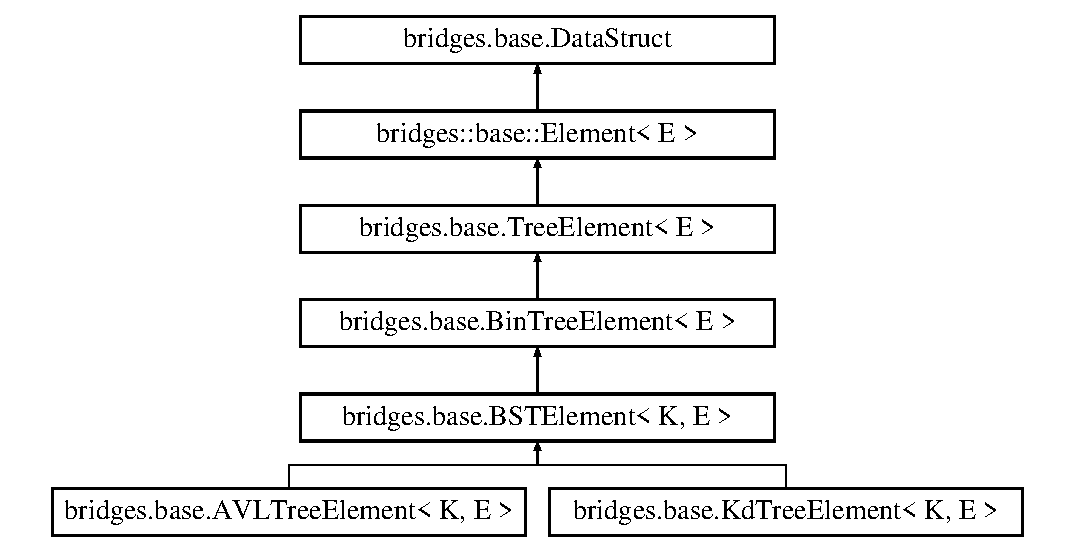
\includegraphics[height=6.000000cm]{classbridges_1_1base_1_1_tree_element}
\end{center}
\end{figure}
\subsection*{Public Member Functions}
\begin{DoxyCompactItemize}
\item 
\mbox{\hyperlink{classbridges_1_1base_1_1_tree_element_ab1af682e9304f5427e308ba5f43d7a9a}{Tree\+Element}} ()
\item 
\mbox{\hyperlink{classbridges_1_1base_1_1_tree_element_a0f17c278536239fb6cba051246ef67a8}{Tree\+Element}} (E e)
\item 
\mbox{\hyperlink{classbridges_1_1base_1_1_tree_element_a476cbeedf2c56f6a40a632035b7d740e}{Tree\+Element}} (String label, E e)
\item 
\mbox{\hyperlink{classbridges_1_1base_1_1_tree_element_aae24dfde287dc0596c69ad853f12f72e}{Tree\+Element}} (\mbox{\hyperlink{classbridges_1_1base_1_1_tree_element}{Tree\+Element}}$<$ E $>$ left, \mbox{\hyperlink{classbridges_1_1base_1_1_tree_element}{Tree\+Element}}$<$ E $>$ right)
\item 
\mbox{\hyperlink{classbridges_1_1base_1_1_tree_element_ace86faa0e65626833c61cc8418cfb1ed}{Tree\+Element}} (E e, \mbox{\hyperlink{classbridges_1_1base_1_1_tree_element}{Tree\+Element}}$<$ E $>$ left, \mbox{\hyperlink{classbridges_1_1base_1_1_tree_element}{Tree\+Element}}$<$ E $>$ right)
\item 
String \mbox{\hyperlink{classbridges_1_1base_1_1_tree_element_a5e0d5f8991d72bd7b0e76d6b0b8662a7}{get\+Data\+Struct\+Type}} ()
\item 
void \mbox{\hyperlink{classbridges_1_1base_1_1_tree_element_a473c29486e99edc725423941b203e939}{add\+Child}} (\mbox{\hyperlink{classbridges_1_1base_1_1_tree_element}{Tree\+Element}}$<$ E $>$ child)
\item 
int \mbox{\hyperlink{classbridges_1_1base_1_1_tree_element_a3722c7cec66ff297f999870df0da3cff}{get\+Number\+Of\+Children}} ()
\item 
void \mbox{\hyperlink{classbridges_1_1base_1_1_tree_element_aefafebb19d64398d150e464e4361ddf0}{set\+Child}} (int index, \mbox{\hyperlink{classbridges_1_1base_1_1_tree_element}{Tree\+Element}}$<$ E $>$ child)
\item 
\mbox{\hyperlink{classbridges_1_1base_1_1_tree_element}{Tree\+Element}}$<$ E $>$ \mbox{\hyperlink{classbridges_1_1base_1_1_tree_element_a4ee40d69ce52fdcac321554564d10aa3}{get\+Child}} (int index)
\item 
String \mbox{\hyperlink{classbridges_1_1base_1_1_tree_element_a674870c91b39fac88d35a569fd505e9b}{get\+Data\+Structure\+Representation}} ()
\end{DoxyCompactItemize}
\subsection*{Additional Inherited Members}


\subsection{Detailed Description}
This class extends \mbox{\hyperlink{classbridges_1_1base_1_1_element}{Element}} to represent general trees with arbitrary number of children. 

\mbox{\hyperlink{classbridges_1_1base_1_1_tree_element}{Tree\+Element}} nodes can have an arbitrary number of child nodes(held in in a vector in the order in which they were added). The visualization of trees assumes that the children are drawn in order from left to right.

Tree Elements have labels (string) that are displayed on the visualization. Elements take an generic object E as a user defined parameter, which can be any native type or object.

Elements contain a visualizer (\mbox{\hyperlink{classbridges_1_1base_1_1_element_visualizer}{Element\+Visualizer}}) object for setting visual attributes (color, shape, opacity, size), necessary for displaying them in a web browser.

Elements also have a \mbox{\hyperlink{classbridges_1_1base_1_1_link_visualizer}{Link\+Visualizer}} object that is used when they are linked to another element, appropriate for setting link attributes, between parent and child nodes.

\begin{DoxyAuthor}{Author}
Kalpathi Subramanian
\end{DoxyAuthor}
\begin{DoxyDate}{Date}
6/22/16, 5/17/17
\end{DoxyDate}

\begin{DoxyParams}{Parameters}
{\em $<$\+E$>$} & The generic parameter object that is part of this element, representing application specific data.\\
\hline
\end{DoxyParams}
\begin{DoxySeeAlso}{See also}
Example tutorial at ~\newline
 ?? 
\end{DoxySeeAlso}


\subsection{Constructor \& Destructor Documentation}
\mbox{\Hypertarget{classbridges_1_1base_1_1_tree_element_ab1af682e9304f5427e308ba5f43d7a9a}\label{classbridges_1_1base_1_1_tree_element_ab1af682e9304f5427e308ba5f43d7a9a}} 
\index{bridges.base.TreeElement$<$ E $>$@{bridges.base.TreeElement$<$ E $>$}!TreeElement@{TreeElement}}
\index{TreeElement@{TreeElement}!bridges.base.TreeElement$<$ E $>$@{bridges.base.TreeElement$<$ E $>$}}
\subsubsection{\texorpdfstring{TreeElement()}{TreeElement()}\hspace{0.1cm}{\footnotesize\ttfamily [1/5]}}
{\footnotesize\ttfamily \mbox{\hyperlink{classbridges_1_1base_1_1_tree_element}{bridges.\+base.\+Tree\+Element}}$<$ E $>$.\mbox{\hyperlink{classbridges_1_1base_1_1_tree_element}{Tree\+Element}} (\begin{DoxyParamCaption}{ }\end{DoxyParamCaption})}

Constructs an empty \mbox{\hyperlink{classbridges_1_1base_1_1_tree_element}{Tree\+Element}} with first two children set to null. \mbox{\Hypertarget{classbridges_1_1base_1_1_tree_element_a0f17c278536239fb6cba051246ef67a8}\label{classbridges_1_1base_1_1_tree_element_a0f17c278536239fb6cba051246ef67a8}} 
\index{bridges.base.TreeElement$<$ E $>$@{bridges.base.TreeElement$<$ E $>$}!TreeElement@{TreeElement}}
\index{TreeElement@{TreeElement}!bridges.base.TreeElement$<$ E $>$@{bridges.base.TreeElement$<$ E $>$}}
\subsubsection{\texorpdfstring{TreeElement()}{TreeElement()}\hspace{0.1cm}{\footnotesize\ttfamily [2/5]}}
{\footnotesize\ttfamily \mbox{\hyperlink{classbridges_1_1base_1_1_tree_element}{bridges.\+base.\+Tree\+Element}}$<$ E $>$.\mbox{\hyperlink{classbridges_1_1base_1_1_tree_element}{Tree\+Element}} (\begin{DoxyParamCaption}\item[{E}]{e }\end{DoxyParamCaption})}

Constructs a \mbox{\hyperlink{classbridges_1_1base_1_1_tree_element}{Tree\+Element}} holding an object \char`\"{}e\char`\"{} with first two children set to null.


\begin{DoxyParams}{Parameters}
{\em e} & the generic object that \mbox{\hyperlink{classbridges_1_1base_1_1_tree_element}{Tree\+Element}} will hold \\
\hline
\end{DoxyParams}
\mbox{\Hypertarget{classbridges_1_1base_1_1_tree_element_a476cbeedf2c56f6a40a632035b7d740e}\label{classbridges_1_1base_1_1_tree_element_a476cbeedf2c56f6a40a632035b7d740e}} 
\index{bridges.base.TreeElement$<$ E $>$@{bridges.base.TreeElement$<$ E $>$}!TreeElement@{TreeElement}}
\index{TreeElement@{TreeElement}!bridges.base.TreeElement$<$ E $>$@{bridges.base.TreeElement$<$ E $>$}}
\subsubsection{\texorpdfstring{TreeElement()}{TreeElement()}\hspace{0.1cm}{\footnotesize\ttfamily [3/5]}}
{\footnotesize\ttfamily \mbox{\hyperlink{classbridges_1_1base_1_1_tree_element}{bridges.\+base.\+Tree\+Element}}$<$ E $>$.\mbox{\hyperlink{classbridges_1_1base_1_1_tree_element}{Tree\+Element}} (\begin{DoxyParamCaption}\item[{String}]{label,  }\item[{E}]{e }\end{DoxyParamCaption})}

Constructs a \mbox{\hyperlink{classbridges_1_1base_1_1_tree_element}{Tree\+Element}} with label set to \char`\"{}label\char`\"{}, holding an object \char`\"{}e\char`\"{}. 
\begin{DoxyParams}{Parameters}
{\em label} & the label of \mbox{\hyperlink{classbridges_1_1base_1_1_tree_element}{Tree\+Element}} that shows up on the Bridges visualization \\
\hline
{\em e} & the generic object that \mbox{\hyperlink{classbridges_1_1base_1_1_tree_element}{Tree\+Element}} will hold \\
\hline
\end{DoxyParams}
\mbox{\Hypertarget{classbridges_1_1base_1_1_tree_element_aae24dfde287dc0596c69ad853f12f72e}\label{classbridges_1_1base_1_1_tree_element_aae24dfde287dc0596c69ad853f12f72e}} 
\index{bridges.base.TreeElement$<$ E $>$@{bridges.base.TreeElement$<$ E $>$}!TreeElement@{TreeElement}}
\index{TreeElement@{TreeElement}!bridges.base.TreeElement$<$ E $>$@{bridges.base.TreeElement$<$ E $>$}}
\subsubsection{\texorpdfstring{TreeElement()}{TreeElement()}\hspace{0.1cm}{\footnotesize\ttfamily [4/5]}}
{\footnotesize\ttfamily \mbox{\hyperlink{classbridges_1_1base_1_1_tree_element}{bridges.\+base.\+Tree\+Element}}$<$ E $>$.\mbox{\hyperlink{classbridges_1_1base_1_1_tree_element}{Tree\+Element}} (\begin{DoxyParamCaption}\item[{\mbox{\hyperlink{classbridges_1_1base_1_1_tree_element}{Tree\+Element}}$<$ E $>$}]{left,  }\item[{\mbox{\hyperlink{classbridges_1_1base_1_1_tree_element}{Tree\+Element}}$<$ E $>$}]{right }\end{DoxyParamCaption})}

Constructs an empty \mbox{\hyperlink{classbridges_1_1base_1_1_tree_element}{Tree\+Element}} left pointer pointing to child 0 and right pointer pointing to child 1.


\begin{DoxyParams}{Parameters}
{\em left} & the \mbox{\hyperlink{classbridges_1_1base_1_1_tree_element}{Tree\+Element}} to be assigned to the child 0 of this \mbox{\hyperlink{classbridges_1_1base_1_1_tree_element}{Tree\+Element}} \\
\hline
{\em right} & the \mbox{\hyperlink{classbridges_1_1base_1_1_tree_element}{Tree\+Element}} to be assigned to the child 1 of this \mbox{\hyperlink{classbridges_1_1base_1_1_tree_element}{Tree\+Element}} \\
\hline
\end{DoxyParams}
\mbox{\Hypertarget{classbridges_1_1base_1_1_tree_element_ace86faa0e65626833c61cc8418cfb1ed}\label{classbridges_1_1base_1_1_tree_element_ace86faa0e65626833c61cc8418cfb1ed}} 
\index{bridges.base.TreeElement$<$ E $>$@{bridges.base.TreeElement$<$ E $>$}!TreeElement@{TreeElement}}
\index{TreeElement@{TreeElement}!bridges.base.TreeElement$<$ E $>$@{bridges.base.TreeElement$<$ E $>$}}
\subsubsection{\texorpdfstring{TreeElement()}{TreeElement()}\hspace{0.1cm}{\footnotesize\ttfamily [5/5]}}
{\footnotesize\ttfamily \mbox{\hyperlink{classbridges_1_1base_1_1_tree_element}{bridges.\+base.\+Tree\+Element}}$<$ E $>$.\mbox{\hyperlink{classbridges_1_1base_1_1_tree_element}{Tree\+Element}} (\begin{DoxyParamCaption}\item[{E}]{e,  }\item[{\mbox{\hyperlink{classbridges_1_1base_1_1_tree_element}{Tree\+Element}}$<$ E $>$}]{left,  }\item[{\mbox{\hyperlink{classbridges_1_1base_1_1_tree_element}{Tree\+Element}}$<$ E $>$}]{right }\end{DoxyParamCaption})}

Constructs a \mbox{\hyperlink{classbridges_1_1base_1_1_tree_element}{Tree\+Element}} holding the object \char`\"{}e\char`\"{}, left pointer pointing to first child and right pointer pointing to second child


\begin{DoxyParams}{Parameters}
{\em e} & the generic object that \mbox{\hyperlink{classbridges_1_1base_1_1_tree_element}{Tree\+Element}} will hold \\
\hline
{\em left} & the \mbox{\hyperlink{classbridges_1_1base_1_1_tree_element}{Tree\+Element}} to be assigned to the first child of this \mbox{\hyperlink{classbridges_1_1base_1_1_tree_element}{Tree\+Element}} \\
\hline
{\em right} & the \mbox{\hyperlink{classbridges_1_1base_1_1_tree_element}{Tree\+Element}} to be assigned to the second child of this \mbox{\hyperlink{classbridges_1_1base_1_1_tree_element}{Tree\+Element}} \\
\hline
\end{DoxyParams}


\subsection{Member Function Documentation}
\mbox{\Hypertarget{classbridges_1_1base_1_1_tree_element_a473c29486e99edc725423941b203e939}\label{classbridges_1_1base_1_1_tree_element_a473c29486e99edc725423941b203e939}} 
\index{bridges.base.TreeElement$<$ E $>$@{bridges.base.TreeElement$<$ E $>$}!addChild@{addChild}}
\index{addChild@{addChild}!bridges.base.TreeElement$<$ E $>$@{bridges.base.TreeElement$<$ E $>$}}
\subsubsection{\texorpdfstring{addChild()}{addChild()}}
{\footnotesize\ttfamily void \mbox{\hyperlink{classbridges_1_1base_1_1_tree_element}{bridges.\+base.\+Tree\+Element}}$<$ E $>$.add\+Child (\begin{DoxyParamCaption}\item[{\mbox{\hyperlink{classbridges_1_1base_1_1_tree_element}{Tree\+Element}}$<$ E $>$}]{child }\end{DoxyParamCaption})}

Adds a child to the node \mbox{\Hypertarget{classbridges_1_1base_1_1_tree_element_a4ee40d69ce52fdcac321554564d10aa3}\label{classbridges_1_1base_1_1_tree_element_a4ee40d69ce52fdcac321554564d10aa3}} 
\index{bridges.base.TreeElement$<$ E $>$@{bridges.base.TreeElement$<$ E $>$}!getChild@{getChild}}
\index{getChild@{getChild}!bridges.base.TreeElement$<$ E $>$@{bridges.base.TreeElement$<$ E $>$}}
\subsubsection{\texorpdfstring{getChild()}{getChild()}}
{\footnotesize\ttfamily \mbox{\hyperlink{classbridges_1_1base_1_1_tree_element}{Tree\+Element}}$<$E$>$ \mbox{\hyperlink{classbridges_1_1base_1_1_tree_element}{bridges.\+base.\+Tree\+Element}}$<$ E $>$.get\+Child (\begin{DoxyParamCaption}\item[{int}]{index }\end{DoxyParamCaption})}

gets a child at a particular index


\begin{DoxyParams}{Parameters}
{\em index} & into the list of children\\
\hline
\end{DoxyParams}
\begin{DoxyReturn}{Returns}
child to be returned 
\end{DoxyReturn}
\mbox{\Hypertarget{classbridges_1_1base_1_1_tree_element_a5e0d5f8991d72bd7b0e76d6b0b8662a7}\label{classbridges_1_1base_1_1_tree_element_a5e0d5f8991d72bd7b0e76d6b0b8662a7}} 
\index{bridges.base.TreeElement$<$ E $>$@{bridges.base.TreeElement$<$ E $>$}!getDataStructType@{getDataStructType}}
\index{getDataStructType@{getDataStructType}!bridges.base.TreeElement$<$ E $>$@{bridges.base.TreeElement$<$ E $>$}}
\subsubsection{\texorpdfstring{getDataStructType()}{getDataStructType()}}
{\footnotesize\ttfamily String \mbox{\hyperlink{classbridges_1_1base_1_1_tree_element}{bridges.\+base.\+Tree\+Element}}$<$ E $>$.get\+Data\+Struct\+Type (\begin{DoxyParamCaption}{ }\end{DoxyParamCaption})}

This method gets the data structure type

\begin{DoxyReturn}{Returns}
The date structure type as a string 
\end{DoxyReturn}
\mbox{\Hypertarget{classbridges_1_1base_1_1_tree_element_a674870c91b39fac88d35a569fd505e9b}\label{classbridges_1_1base_1_1_tree_element_a674870c91b39fac88d35a569fd505e9b}} 
\index{bridges.base.TreeElement$<$ E $>$@{bridges.base.TreeElement$<$ E $>$}!getDataStructureRepresentation@{getDataStructureRepresentation}}
\index{getDataStructureRepresentation@{getDataStructureRepresentation}!bridges.base.TreeElement$<$ E $>$@{bridges.base.TreeElement$<$ E $>$}}
\subsubsection{\texorpdfstring{getDataStructureRepresentation()}{getDataStructureRepresentation()}}
{\footnotesize\ttfamily String \mbox{\hyperlink{classbridges_1_1base_1_1_tree_element}{bridges.\+base.\+Tree\+Element}}$<$ E $>$.get\+Data\+Structure\+Representation (\begin{DoxyParamCaption}{ }\end{DoxyParamCaption})}

Get hierarchical J\+S\+ON of the tree representation

\begin{DoxyReturn}{Returns}
the J\+S\+ON string 
\end{DoxyReturn}
\mbox{\Hypertarget{classbridges_1_1base_1_1_tree_element_a3722c7cec66ff297f999870df0da3cff}\label{classbridges_1_1base_1_1_tree_element_a3722c7cec66ff297f999870df0da3cff}} 
\index{bridges.base.TreeElement$<$ E $>$@{bridges.base.TreeElement$<$ E $>$}!getNumberOfChildren@{getNumberOfChildren}}
\index{getNumberOfChildren@{getNumberOfChildren}!bridges.base.TreeElement$<$ E $>$@{bridges.base.TreeElement$<$ E $>$}}
\subsubsection{\texorpdfstring{getNumberOfChildren()}{getNumberOfChildren()}}
{\footnotesize\ttfamily int \mbox{\hyperlink{classbridges_1_1base_1_1_tree_element}{bridges.\+base.\+Tree\+Element}}$<$ E $>$.get\+Number\+Of\+Children (\begin{DoxyParamCaption}{ }\end{DoxyParamCaption})}

Returns the number of children at this node

\begin{DoxyReturn}{Returns}
number of children 
\end{DoxyReturn}
\mbox{\Hypertarget{classbridges_1_1base_1_1_tree_element_aefafebb19d64398d150e464e4361ddf0}\label{classbridges_1_1base_1_1_tree_element_aefafebb19d64398d150e464e4361ddf0}} 
\index{bridges.base.TreeElement$<$ E $>$@{bridges.base.TreeElement$<$ E $>$}!setChild@{setChild}}
\index{setChild@{setChild}!bridges.base.TreeElement$<$ E $>$@{bridges.base.TreeElement$<$ E $>$}}
\subsubsection{\texorpdfstring{setChild()}{setChild()}}
{\footnotesize\ttfamily void \mbox{\hyperlink{classbridges_1_1base_1_1_tree_element}{bridges.\+base.\+Tree\+Element}}$<$ E $>$.set\+Child (\begin{DoxyParamCaption}\item[{int}]{index,  }\item[{\mbox{\hyperlink{classbridges_1_1base_1_1_tree_element}{Tree\+Element}}$<$ E $>$}]{child }\end{DoxyParamCaption})}

adds a child to the node -\/ will be added at the next open position


\begin{DoxyParams}{Parameters}
{\em child} & to be added\\
\hline
\end{DoxyParams}
\begin{DoxyReturn}{Returns}
none 
\end{DoxyReturn}


The documentation for this class was generated from the following file\+:\begin{DoxyCompactItemize}
\item 
/\+Users/kalpathi/gr/bridges/java/src/main/java/bridges/base/\mbox{\hyperlink{_tree_element_8java}{Tree\+Element.\+java}}\end{DoxyCompactItemize}

\hypertarget{classbridges_1_1validation_1_1_validation}{}\section{bridges.\+validation.\+Validation Class Reference}
\label{classbridges_1_1validation_1_1_validation}\index{bridges.\+validation.\+Validation@{bridges.\+validation.\+Validation}}
\subsection*{Static Public Member Functions}
\begin{DoxyCompactItemize}
\item 
static void \hyperlink{classbridges_1_1validation_1_1_validation_ae529d673f5b86b457ed7b7d4d80a9dbf}{validate\+Color} (String color)  throws Invalid\+Value\+Exception 
\item 
static void \hyperlink{classbridges_1_1validation_1_1_validation_a81a0f7eda485bb1c2d786d78936ca4b9}{validate\+Shape} (String shape)
\item 
static void \hyperlink{classbridges_1_1validation_1_1_validation_ab6cd587755b3128031da73a35895f666}{validate\+Opacity} (double val)
\item 
static void \hyperlink{classbridges_1_1validation_1_1_validation_ad031369dbb08eadfc698e5e9e7e59605}{validate\+Size} (double val)
\item 
static void \hyperlink{classbridges_1_1validation_1_1_validation_a2c0f34fbcf1315301aefa02818d379f3}{validate\+Thickness} (double val)
\item 
static void \hyperlink{classbridges_1_1validation_1_1_validation_a0a3b322af9a6815fd1acba481858d0e3}{validate\+\_\+\+A\+D\+T\+\_\+size} (int i)
\end{DoxyCompactItemize}
\subsection*{Static Public Attributes}
\begin{DoxyCompactItemize}
\item 
static final Set$<$ String $>$ \hyperlink{classbridges_1_1validation_1_1_validation_a580ab67e2b85bc3ee6ee8af138180624}{C\+O\+L\+O\+R\+\_\+\+N\+A\+M\+E\+S} = new Hash\+Set$<$String$>$()
\item 
static final Set$<$ Pattern $>$ \hyperlink{classbridges_1_1validation_1_1_validation_a16e87ec9f7fe5ef76aea76277a612c76}{C\+O\+L\+O\+R\+\_\+\+P\+A\+T\+T\+E\+R\+N\+S} = new Hash\+Set$<$Pattern$>$()
\item 
static final Set$<$ String $>$ \hyperlink{classbridges_1_1validation_1_1_validation_a43f1f9efc20d0086b7fcfa9b40bd7146}{N\+O\+D\+E\+\_\+\+S\+H\+A\+P\+E\+S} = new Hash\+Set$<$String$>$()
\end{DoxyCompactItemize}


\subsection{Member Function Documentation}
\hypertarget{classbridges_1_1validation_1_1_validation_a0a3b322af9a6815fd1acba481858d0e3}{}\index{bridges\+::validation\+::\+Validation@{bridges\+::validation\+::\+Validation}!validate\+\_\+\+A\+D\+T\+\_\+size@{validate\+\_\+\+A\+D\+T\+\_\+size}}
\index{validate\+\_\+\+A\+D\+T\+\_\+size@{validate\+\_\+\+A\+D\+T\+\_\+size}!bridges\+::validation\+::\+Validation@{bridges\+::validation\+::\+Validation}}
\subsubsection[{validate\+\_\+\+A\+D\+T\+\_\+size(int i)}]{\setlength{\rightskip}{0pt plus 5cm}static void bridges.\+validation.\+Validation.\+validate\+\_\+\+A\+D\+T\+\_\+size (
\begin{DoxyParamCaption}
\item[{int}]{i}
\end{DoxyParamCaption}
)\hspace{0.3cm}{\ttfamily [static]}}\label{classbridges_1_1validation_1_1_validation_a0a3b322af9a6815fd1acba481858d0e3}
\hypertarget{classbridges_1_1validation_1_1_validation_ae529d673f5b86b457ed7b7d4d80a9dbf}{}\index{bridges\+::validation\+::\+Validation@{bridges\+::validation\+::\+Validation}!validate\+Color@{validate\+Color}}
\index{validate\+Color@{validate\+Color}!bridges\+::validation\+::\+Validation@{bridges\+::validation\+::\+Validation}}
\subsubsection[{validate\+Color(\+String color)}]{\setlength{\rightskip}{0pt plus 5cm}static void bridges.\+validation.\+Validation.\+validate\+Color (
\begin{DoxyParamCaption}
\item[{String}]{color}
\end{DoxyParamCaption}
) throws {\bf Invalid\+Value\+Exception}\hspace{0.3cm}{\ttfamily [static]}}\label{classbridges_1_1validation_1_1_validation_ae529d673f5b86b457ed7b7d4d80a9dbf}
Determine if a color is supported by C\+S\+S.

This method only supports a subject of C\+S\+S (yet). (1) 173 C\+S\+S extended color names, (2) \#\+R\+R\+G\+G\+B\+B or \#\+R\+G\+B, where R, G and B are red, green, blue values as hexadecimal digits.

This method does not check for null because null has special meaning.


\begin{DoxyParams}{Parameters}
{\em color} & \\
\hline
\end{DoxyParams}
\begin{DoxyReturn}{Returns}
whether the color is valid 
\end{DoxyReturn}
\hypertarget{classbridges_1_1validation_1_1_validation_ab6cd587755b3128031da73a35895f666}{}\index{bridges\+::validation\+::\+Validation@{bridges\+::validation\+::\+Validation}!validate\+Opacity@{validate\+Opacity}}
\index{validate\+Opacity@{validate\+Opacity}!bridges\+::validation\+::\+Validation@{bridges\+::validation\+::\+Validation}}
\subsubsection[{validate\+Opacity(double val)}]{\setlength{\rightskip}{0pt plus 5cm}static void bridges.\+validation.\+Validation.\+validate\+Opacity (
\begin{DoxyParamCaption}
\item[{double}]{val}
\end{DoxyParamCaption}
)\hspace{0.3cm}{\ttfamily [static]}}\label{classbridges_1_1validation_1_1_validation_ab6cd587755b3128031da73a35895f666}
Determines if the value passed is an acceptable value to set the opacity to.


\begin{DoxyParams}{Parameters}
{\em val} & \\
\hline
\end{DoxyParams}
\hypertarget{classbridges_1_1validation_1_1_validation_a81a0f7eda485bb1c2d786d78936ca4b9}{}\index{bridges\+::validation\+::\+Validation@{bridges\+::validation\+::\+Validation}!validate\+Shape@{validate\+Shape}}
\index{validate\+Shape@{validate\+Shape}!bridges\+::validation\+::\+Validation@{bridges\+::validation\+::\+Validation}}
\subsubsection[{validate\+Shape(\+String shape)}]{\setlength{\rightskip}{0pt plus 5cm}static void bridges.\+validation.\+Validation.\+validate\+Shape (
\begin{DoxyParamCaption}
\item[{String}]{shape}
\end{DoxyParamCaption}
)\hspace{0.3cm}{\ttfamily [static]}}\label{classbridges_1_1validation_1_1_validation_a81a0f7eda485bb1c2d786d78936ca4b9}
Determines if the shape is supported.


\begin{DoxyParams}{Parameters}
{\em shape} & \\
\hline
\end{DoxyParams}
\hypertarget{classbridges_1_1validation_1_1_validation_ad031369dbb08eadfc698e5e9e7e59605}{}\index{bridges\+::validation\+::\+Validation@{bridges\+::validation\+::\+Validation}!validate\+Size@{validate\+Size}}
\index{validate\+Size@{validate\+Size}!bridges\+::validation\+::\+Validation@{bridges\+::validation\+::\+Validation}}
\subsubsection[{validate\+Size(double val)}]{\setlength{\rightskip}{0pt plus 5cm}static void bridges.\+validation.\+Validation.\+validate\+Size (
\begin{DoxyParamCaption}
\item[{double}]{val}
\end{DoxyParamCaption}
)\hspace{0.3cm}{\ttfamily [static]}}\label{classbridges_1_1validation_1_1_validation_ad031369dbb08eadfc698e5e9e7e59605}
Determines if the size value passed is an acceptable value to set the size to.


\begin{DoxyParams}{Parameters}
{\em val} & \\
\hline
\end{DoxyParams}
\hypertarget{classbridges_1_1validation_1_1_validation_a2c0f34fbcf1315301aefa02818d379f3}{}\index{bridges\+::validation\+::\+Validation@{bridges\+::validation\+::\+Validation}!validate\+Thickness@{validate\+Thickness}}
\index{validate\+Thickness@{validate\+Thickness}!bridges\+::validation\+::\+Validation@{bridges\+::validation\+::\+Validation}}
\subsubsection[{validate\+Thickness(double val)}]{\setlength{\rightskip}{0pt plus 5cm}static void bridges.\+validation.\+Validation.\+validate\+Thickness (
\begin{DoxyParamCaption}
\item[{double}]{val}
\end{DoxyParamCaption}
)\hspace{0.3cm}{\ttfamily [static]}}\label{classbridges_1_1validation_1_1_validation_a2c0f34fbcf1315301aefa02818d379f3}
Determines if the link thickness value passed is an acceptable value to set the size to.


\begin{DoxyParams}{Parameters}
{\em val} & \\
\hline
\end{DoxyParams}


\subsection{Member Data Documentation}
\hypertarget{classbridges_1_1validation_1_1_validation_a580ab67e2b85bc3ee6ee8af138180624}{}\index{bridges\+::validation\+::\+Validation@{bridges\+::validation\+::\+Validation}!C\+O\+L\+O\+R\+\_\+\+N\+A\+M\+E\+S@{C\+O\+L\+O\+R\+\_\+\+N\+A\+M\+E\+S}}
\index{C\+O\+L\+O\+R\+\_\+\+N\+A\+M\+E\+S@{C\+O\+L\+O\+R\+\_\+\+N\+A\+M\+E\+S}!bridges\+::validation\+::\+Validation@{bridges\+::validation\+::\+Validation}}
\subsubsection[{C\+O\+L\+O\+R\+\_\+\+N\+A\+M\+E\+S}]{\setlength{\rightskip}{0pt plus 5cm}final Set$<$String$>$ bridges.\+validation.\+Validation.\+C\+O\+L\+O\+R\+\_\+\+N\+A\+M\+E\+S = new Hash\+Set$<$String$>$()\hspace{0.3cm}{\ttfamily [static]}}\label{classbridges_1_1validation_1_1_validation_a580ab67e2b85bc3ee6ee8af138180624}
\hypertarget{classbridges_1_1validation_1_1_validation_a16e87ec9f7fe5ef76aea76277a612c76}{}\index{bridges\+::validation\+::\+Validation@{bridges\+::validation\+::\+Validation}!C\+O\+L\+O\+R\+\_\+\+P\+A\+T\+T\+E\+R\+N\+S@{C\+O\+L\+O\+R\+\_\+\+P\+A\+T\+T\+E\+R\+N\+S}}
\index{C\+O\+L\+O\+R\+\_\+\+P\+A\+T\+T\+E\+R\+N\+S@{C\+O\+L\+O\+R\+\_\+\+P\+A\+T\+T\+E\+R\+N\+S}!bridges\+::validation\+::\+Validation@{bridges\+::validation\+::\+Validation}}
\subsubsection[{C\+O\+L\+O\+R\+\_\+\+P\+A\+T\+T\+E\+R\+N\+S}]{\setlength{\rightskip}{0pt plus 5cm}final Set$<$Pattern$>$ bridges.\+validation.\+Validation.\+C\+O\+L\+O\+R\+\_\+\+P\+A\+T\+T\+E\+R\+N\+S = new Hash\+Set$<$Pattern$>$()\hspace{0.3cm}{\ttfamily [static]}}\label{classbridges_1_1validation_1_1_validation_a16e87ec9f7fe5ef76aea76277a612c76}
\hypertarget{classbridges_1_1validation_1_1_validation_a43f1f9efc20d0086b7fcfa9b40bd7146}{}\index{bridges\+::validation\+::\+Validation@{bridges\+::validation\+::\+Validation}!N\+O\+D\+E\+\_\+\+S\+H\+A\+P\+E\+S@{N\+O\+D\+E\+\_\+\+S\+H\+A\+P\+E\+S}}
\index{N\+O\+D\+E\+\_\+\+S\+H\+A\+P\+E\+S@{N\+O\+D\+E\+\_\+\+S\+H\+A\+P\+E\+S}!bridges\+::validation\+::\+Validation@{bridges\+::validation\+::\+Validation}}
\subsubsection[{N\+O\+D\+E\+\_\+\+S\+H\+A\+P\+E\+S}]{\setlength{\rightskip}{0pt plus 5cm}final Set$<$String$>$ bridges.\+validation.\+Validation.\+N\+O\+D\+E\+\_\+\+S\+H\+A\+P\+E\+S = new Hash\+Set$<$String$>$()\hspace{0.3cm}{\ttfamily [static]}}\label{classbridges_1_1validation_1_1_validation_a43f1f9efc20d0086b7fcfa9b40bd7146}


The documentation for this class was generated from the following file\+:\begin{DoxyCompactItemize}
\item 
/\+Users/krs/gr/bridges/client/java/src/main/java/bridges/validation/\hyperlink{_validation_8java}{Validation.\+java}\end{DoxyCompactItemize}

\chapter{File Documentation}
\hypertarget{_array_8java}{}\section{/\+Users/kalpathi/gr/bridges/client/java/bridges-\/17/src/main/java/bridges/base/\+Array.java File Reference}
\label{_array_8java}\index{/\+Users/kalpathi/gr/bridges/client/java/bridges-\/17/src/main/java/bridges/base/\+Array.\+java@{/\+Users/kalpathi/gr/bridges/client/java/bridges-\/17/src/main/java/bridges/base/\+Array.\+java}}
\subsection*{Classes}
\begin{DoxyCompactItemize}
\item 
class \mbox{\hyperlink{classbridges_1_1base_1_1_array}{bridges.\+base.\+Array$<$ E $>$}}
\begin{DoxyCompactList}\small\item\em This class can be used to create arrays of type Element$<$\+E$>$. \end{DoxyCompactList}\end{DoxyCompactItemize}
\subsection*{Packages}
\begin{DoxyCompactItemize}
\item 
package \mbox{\hyperlink{namespacebridges_1_1base}{bridges.\+base}}
\end{DoxyCompactItemize}

\hypertarget{_array1_d_8java}{}\section{/home/erik/work/bridges/bridges-\/java/src/main/java/bridges/base/\+Array1D.java File Reference}
\label{_array1_d_8java}\index{/home/erik/work/bridges/bridges-\/java/src/main/java/bridges/base/\+Array1\+D.\+java@{/home/erik/work/bridges/bridges-\/java/src/main/java/bridges/base/\+Array1\+D.\+java}}
\subsection*{Classes}
\begin{DoxyCompactItemize}
\item 
class \hyperlink{classbridges_1_1base_1_1_array1_d}{bridges.\+base.\+Array1\+D$<$ E $>$}
\begin{DoxyCompactList}\small\item\em This is a class can be used to create 1 dimensional arrays of type Element$<$\+E$>$. \end{DoxyCompactList}\end{DoxyCompactItemize}
\subsection*{Packages}
\begin{DoxyCompactItemize}
\item 
package \hyperlink{namespacebridges_1_1base}{bridges.\+base}
\end{DoxyCompactItemize}

\hypertarget{_array2_d_8java}{}\section{/home/erik/work/bridges/bridges-\/java/src/main/java/bridges/base/\+Array2D.java File Reference}
\label{_array2_d_8java}\index{/home/erik/work/bridges/bridges-\/java/src/main/java/bridges/base/\+Array2\+D.\+java@{/home/erik/work/bridges/bridges-\/java/src/main/java/bridges/base/\+Array2\+D.\+java}}
\subsection*{Classes}
\begin{DoxyCompactItemize}
\item 
class \hyperlink{classbridges_1_1base_1_1_array2_d}{bridges.\+base.\+Array2\+D$<$ E $>$}
\begin{DoxyCompactList}\small\item\em This class can be used to create arrays of type Element$<$\+E$>$. \end{DoxyCompactList}\end{DoxyCompactItemize}
\subsection*{Packages}
\begin{DoxyCompactItemize}
\item 
package \hyperlink{namespacebridges_1_1base}{bridges.\+base}
\end{DoxyCompactItemize}

\hypertarget{_array3_d_8java}{}\doxysection{/\+Users/kalpathi/gr/bridges/client/java/src/main/java/bridges/base/\+Array3D.java File Reference}
\label{_array3_d_8java}\index{/Users/kalpathi/gr/bridges/client/java/src/main/java/bridges/base/Array3D.java@{/Users/kalpathi/gr/bridges/client/java/src/main/java/bridges/base/Array3D.java}}
\doxysubsection*{Classes}
\begin{DoxyCompactItemize}
\item 
class \mbox{\hyperlink{classbridges_1_1base_1_1_array3_d}{bridges.\+base.\+Array3\+D$<$ E $>$}}
\begin{DoxyCompactList}\small\item\em This class can be used to create two dimensional arrays of type Element$<$\+E$>$. \end{DoxyCompactList}\end{DoxyCompactItemize}
\doxysubsection*{Packages}
\begin{DoxyCompactItemize}
\item 
package \mbox{\hyperlink{namespacebridges_1_1base}{bridges.\+base}}
\end{DoxyCompactItemize}

\hypertarget{_audio_channel_8java}{}\section{/home/erik/work/bridges/bridges-\/java/src/main/java/bridges/base/\+Audio\+Channel.java File Reference}
\label{_audio_channel_8java}\index{/home/erik/work/bridges/bridges-\/java/src/main/java/bridges/base/\+Audio\+Channel.\+java@{/home/erik/work/bridges/bridges-\/java/src/main/java/bridges/base/\+Audio\+Channel.\+java}}
\subsection*{Classes}
\begin{DoxyCompactItemize}
\item 
class \hyperlink{classbridges_1_1base_1_1_audio_channel}{bridges.\+base.\+Audio\+Channel}
\end{DoxyCompactItemize}
\subsection*{Packages}
\begin{DoxyCompactItemize}
\item 
package \hyperlink{namespacebridges_1_1base}{bridges.\+base}
\end{DoxyCompactItemize}

\hypertarget{_audio_clip_8java}{}\section{/home/erik/work/bridges/bridges-\/java/src/main/java/bridges/base/\+Audio\+Clip.java File Reference}
\label{_audio_clip_8java}\index{/home/erik/work/bridges/bridges-\/java/src/main/java/bridges/base/\+Audio\+Clip.\+java@{/home/erik/work/bridges/bridges-\/java/src/main/java/bridges/base/\+Audio\+Clip.\+java}}
\subsection*{Classes}
\begin{DoxyCompactItemize}
\item 
class \hyperlink{classbridges_1_1base_1_1_audio_clip}{bridges.\+base.\+Audio\+Clip}
\end{DoxyCompactItemize}
\subsection*{Packages}
\begin{DoxyCompactItemize}
\item 
package \hyperlink{namespacebridges_1_1base}{bridges.\+base}
\end{DoxyCompactItemize}

\hypertarget{_a_v_l_tree_element_8java}{}\section{link/base/\+A\+V\+L\+Tree\+Element.java File Reference}
\label{_a_v_l_tree_element_8java}\index{link/base/\+A\+V\+L\+Tree\+Element.\+java@{link/base/\+A\+V\+L\+Tree\+Element.\+java}}
\subsection*{Classes}
\begin{DoxyCompactItemize}
\item 
class \hyperlink{classbridges_1_1base_1_1_a_v_l_tree_element}{bridges.\+base.\+A\+V\+L\+Tree\+Element$<$ K, E $>$}
\end{DoxyCompactItemize}
\subsection*{Packages}
\begin{DoxyCompactItemize}
\item 
package \hyperlink{namespacebridges_1_1base}{bridges.\+base}
\end{DoxyCompactItemize}

\hypertarget{_bin_tree_element_8java}{}\section{/\+Users/kalpathi/gr/bridges/bridges17/java/src/main/java/bridges/base/\+Bin\+Tree\+Element.java File Reference}
\label{_bin_tree_element_8java}\index{/\+Users/kalpathi/gr/bridges/bridges17/java/src/main/java/bridges/base/\+Bin\+Tree\+Element.\+java@{/\+Users/kalpathi/gr/bridges/bridges17/java/src/main/java/bridges/base/\+Bin\+Tree\+Element.\+java}}
\subsection*{Classes}
\begin{DoxyCompactItemize}
\item 
class \hyperlink{classbridges_1_1base_1_1_bin_tree_element}{bridges.\+base.\+Bin\+Tree\+Element$<$ E $>$}
\begin{DoxyCompactList}\small\item\em This class is extended from the \hyperlink{classbridges_1_1base_1_1_tree_element}{Tree\+Element} class and can be used to create binary tree element objects. \end{DoxyCompactList}\end{DoxyCompactItemize}
\subsection*{Packages}
\begin{DoxyCompactItemize}
\item 
package \hyperlink{namespacebridges_1_1base}{bridges.\+base}
\end{DoxyCompactItemize}

\hypertarget{_b_s_t_element_8java}{}\section{/\+Users/krs/gr/bridges/client/java/src/main/java/bridges/base/\+B\+S\+T\+Element.java File Reference}
\label{_b_s_t_element_8java}\index{/\+Users/krs/gr/bridges/client/java/src/main/java/bridges/base/\+B\+S\+T\+Element.\+java@{/\+Users/krs/gr/bridges/client/java/src/main/java/bridges/base/\+B\+S\+T\+Element.\+java}}
\subsection*{Classes}
\begin{DoxyCompactItemize}
\item 
class \hyperlink{classbridges_1_1base_1_1_b_s_t_element}{bridges.\+base.\+B\+S\+T\+Element$<$ K, E $>$}
\begin{DoxyCompactList}\small\item\em The \hyperlink{classbridges_1_1base_1_1_b_s_t_element}{B\+S\+T\+Element} class is the building block for creating binary search trees. \end{DoxyCompactList}\end{DoxyCompactItemize}
\subsection*{Packages}
\begin{DoxyCompactItemize}
\item 
package \hyperlink{namespacebridges_1_1base}{bridges.\+base}
\end{DoxyCompactItemize}

\hypertarget{_circ_d_lelement_8java}{}\section{/\+Users/kalpathi/gr/bridges/client/java/bridges16/src/main/java/edu/uncc/cs/bridges\+\_\+v21/base/\+Circ\+D\+Lelement.java File Reference}
\label{_circ_d_lelement_8java}\index{/\+Users/kalpathi/gr/bridges/client/java/bridges16/src/main/java/edu/uncc/cs/bridges\+\_\+v21/base/\+Circ\+D\+Lelement.\+java@{/\+Users/kalpathi/gr/bridges/client/java/bridges16/src/main/java/edu/uncc/cs/bridges\+\_\+v21/base/\+Circ\+D\+Lelement.\+java}}
\subsection*{Classes}
\begin{DoxyCompactItemize}
\item 
class \hyperlink{classbridges_1_1base_1_1_circ_d_lelement}{bridges.\+base.\+Circ\+D\+Lelement$<$ E $>$}
\begin{DoxyCompactList}\small\item\em This class can be used to instantiate Circular Doubly Linked List Elements. \end{DoxyCompactList}\end{DoxyCompactItemize}
\subsection*{Packages}
\begin{DoxyCompactItemize}
\item 
package \hyperlink{namespacebridges_1_1base}{bridges.\+base}
\end{DoxyCompactItemize}

\hypertarget{_circle_8java}{}\doxysection{/\+Users/kalpathi/gr/bridges/client/java/src/main/java/bridges/base/\+Circle.java File Reference}
\label{_circle_8java}\index{/Users/kalpathi/gr/bridges/client/java/src/main/java/bridges/base/Circle.java@{/Users/kalpathi/gr/bridges/client/java/src/main/java/bridges/base/Circle.java}}
\doxysubsection*{Classes}
\begin{DoxyCompactItemize}
\item 
class \mbox{\hyperlink{classbridges_1_1base_1_1_circle}{bridges.\+base.\+Circle}}
\begin{DoxyCompactList}\small\item\em This class defines a circle and is part of the symbol collection. A circle has a center and radius. \end{DoxyCompactList}\end{DoxyCompactItemize}
\doxysubsection*{Packages}
\begin{DoxyCompactItemize}
\item 
package \mbox{\hyperlink{namespacebridges_1_1base}{bridges.\+base}}
\end{DoxyCompactItemize}

\hypertarget{_circ_s_lelement_8java}{}\section{/\+Users/kalpathi/gr/bridges/java/src/main/java/bridges/base/\+Circ\+S\+Lelement.java File Reference}
\label{_circ_s_lelement_8java}\index{/Users/kalpathi/gr/bridges/java/src/main/java/bridges/base/CircSLelement.java@{/Users/kalpathi/gr/bridges/java/src/main/java/bridges/base/CircSLelement.java}}
\subsection*{Classes}
\begin{DoxyCompactItemize}
\item 
class \mbox{\hyperlink{classbridges_1_1base_1_1_circ_s_lelement}{bridges.\+base.\+Circ\+S\+Lelement$<$ E $>$}}
\begin{DoxyCompactList}\small\item\em This class can be used to instantiate Singly Linked Circular List Elements. \end{DoxyCompactList}\end{DoxyCompactItemize}
\subsection*{Packages}
\begin{DoxyCompactItemize}
\item 
package \mbox{\hyperlink{namespacebridges_1_1base}{bridges.\+base}}
\end{DoxyCompactItemize}

\hypertarget{_color_8java}{}\section{/\+Users/kalpathi/gr/bridges/client/java/bridges-\/17/src/main/java/bridges/base/\+Color.java File Reference}
\label{_color_8java}\index{/\+Users/kalpathi/gr/bridges/client/java/bridges-\/17/src/main/java/bridges/base/\+Color.\+java@{/\+Users/kalpathi/gr/bridges/client/java/bridges-\/17/src/main/java/bridges/base/\+Color.\+java}}
\subsection*{Classes}
\begin{DoxyCompactItemize}
\item 
class \mbox{\hyperlink{classbridges_1_1base_1_1_color}{bridges.\+base.\+Color}}
\begin{DoxyCompactList}\small\item\em This class is used to represent colors in B\+R\+I\+D\+G\+ES. \end{DoxyCompactList}\end{DoxyCompactItemize}
\subsection*{Packages}
\begin{DoxyCompactItemize}
\item 
package \mbox{\hyperlink{namespacebridges_1_1base}{bridges.\+base}}
\end{DoxyCompactItemize}

\hypertarget{_color_grid_8java}{}\section{/\+Users/kalpathi/gr/bridges/bridges17/java/src/main/java/bridges/base/\+Color\+Grid.java File Reference}
\label{_color_grid_8java}\index{/\+Users/kalpathi/gr/bridges/bridges17/java/src/main/java/bridges/base/\+Color\+Grid.\+java@{/\+Users/kalpathi/gr/bridges/bridges17/java/src/main/java/bridges/base/\+Color\+Grid.\+java}}
\subsection*{Classes}
\begin{DoxyCompactItemize}
\item 
class \hyperlink{classbridges_1_1base_1_1_color_grid}{bridges.\+base.\+Color\+Grid}
\begin{DoxyCompactList}\small\item\em This is a class in B\+R\+I\+D\+G\+E\+S for representing an (n x n) grid. \end{DoxyCompactList}\end{DoxyCompactItemize}
\subsection*{Packages}
\begin{DoxyCompactItemize}
\item 
package \hyperlink{namespacebridges_1_1base}{bridges.\+base}
\end{DoxyCompactItemize}

\hypertarget{_data_struct_8java}{}\section{/\+Users/kalpathi/gr/bridges/client/java/bridges-\/17/src/main/java/bridges/base/\+Data\+Struct.java File Reference}
\label{_data_struct_8java}\index{/\+Users/kalpathi/gr/bridges/client/java/bridges-\/17/src/main/java/bridges/base/\+Data\+Struct.\+java@{/\+Users/kalpathi/gr/bridges/client/java/bridges-\/17/src/main/java/bridges/base/\+Data\+Struct.\+java}}
\subsection*{Classes}
\begin{DoxyCompactItemize}
\item 
class \mbox{\hyperlink{classbridges_1_1base_1_1_data_struct}{bridges.\+base.\+Data\+Struct}}
\begin{DoxyCompactList}\small\item\em This is an abstract super class that is extended by all Bridges subclasses and provides some methods that are used universally across B\+R\+I\+D\+G\+ES. \end{DoxyCompactList}\end{DoxyCompactItemize}
\subsection*{Packages}
\begin{DoxyCompactItemize}
\item 
package \mbox{\hyperlink{namespacebridges_1_1base}{bridges.\+base}}
\end{DoxyCompactItemize}

\hypertarget{_d_lelement_8java}{}\doxysection{/\+Users/kalpathi/gr/bridges/client/java/src/main/java/bridges/base/\+D\+Lelement.java File Reference}
\label{_d_lelement_8java}\index{/Users/kalpathi/gr/bridges/client/java/src/main/java/bridges/base/DLelement.java@{/Users/kalpathi/gr/bridges/client/java/src/main/java/bridges/base/DLelement.java}}
\doxysubsection*{Classes}
\begin{DoxyCompactItemize}
\item 
class \mbox{\hyperlink{classbridges_1_1base_1_1_d_lelement}{bridges.\+base.\+D\+Lelement$<$ E $>$}}
\begin{DoxyCompactList}\small\item\em This class is used to create doubly linked element objects. \end{DoxyCompactList}\end{DoxyCompactItemize}
\doxysubsection*{Packages}
\begin{DoxyCompactItemize}
\item 
package \mbox{\hyperlink{namespacebridges_1_1base}{bridges.\+base}}
\end{DoxyCompactItemize}

\hypertarget{_edge_8java}{}\section{link/base/\+Edge.java File Reference}
\label{_edge_8java}\index{link/base/\+Edge.\+java@{link/base/\+Edge.\+java}}
\subsection*{Classes}
\begin{DoxyCompactItemize}
\item 
class \hyperlink{classbridges_1_1base_1_1_edge}{bridges.\+base.\+Edge$<$ K $>$}
\begin{DoxyCompactList}\small\item\em This class is used to represent the edges in a graph and will appear as links in the B\+R\+I\+D\+G\+ES graph visualization. \end{DoxyCompactList}\end{DoxyCompactItemize}
\subsection*{Packages}
\begin{DoxyCompactItemize}
\item 
package \hyperlink{namespacebridges_1_1base}{bridges.\+base}
\end{DoxyCompactItemize}

\hypertarget{_element_8java}{}\section{/\+Users/kalpathi/gr/bridges/bridges17/java/src/main/java/bridges/base/\+Element.java File Reference}
\label{_element_8java}\index{/\+Users/kalpathi/gr/bridges/bridges17/java/src/main/java/bridges/base/\+Element.\+java@{/\+Users/kalpathi/gr/bridges/bridges17/java/src/main/java/bridges/base/\+Element.\+java}}
\subsection*{Classes}
\begin{DoxyCompactItemize}
\item 
class \hyperlink{classbridges_1_1base_1_1_element}{bridges.\+base.\+Element$<$ E $>$}
\begin{DoxyCompactList}\small\item\em This is the main superclass in B\+R\+I\+D\+G\+E\+S for deriving a number of objects used in building arrays, lists, trees and graph data structures. \end{DoxyCompactList}\end{DoxyCompactItemize}
\subsection*{Packages}
\begin{DoxyCompactItemize}
\item 
package \hyperlink{namespacebridges_1_1base}{bridges.\+base}
\end{DoxyCompactItemize}

\hypertarget{_element_visualizer_8java}{}\doxysection{/\+Users/kalpathi/gr/bridges/client/java/src/main/java/bridges/base/\+Element\+Visualizer.java File Reference}
\label{_element_visualizer_8java}\index{/Users/kalpathi/gr/bridges/client/java/src/main/java/bridges/base/ElementVisualizer.java@{/Users/kalpathi/gr/bridges/client/java/src/main/java/bridges/base/ElementVisualizer.java}}
\doxysubsection*{Classes}
\begin{DoxyCompactItemize}
\item 
class \mbox{\hyperlink{classbridges_1_1base_1_1_element_visualizer}{bridges.\+base.\+Element\+Visualizer}}
\begin{DoxyCompactList}\small\item\em This class maintains the visual attributes of each B\+R\+I\+D\+G\+ES element. \end{DoxyCompactList}\end{DoxyCompactItemize}
\doxysubsection*{Packages}
\begin{DoxyCompactItemize}
\item 
package \mbox{\hyperlink{namespacebridges_1_1base}{bridges.\+base}}
\end{DoxyCompactItemize}

\hypertarget{_game_cell_8java}{}\section{/\+Users/kalpathi/gr/bridges/java/src/main/java/bridges/base/\+Game\+Cell.java File Reference}
\label{_game_cell_8java}\index{/Users/kalpathi/gr/bridges/java/src/main/java/bridges/base/GameCell.java@{/Users/kalpathi/gr/bridges/java/src/main/java/bridges/base/GameCell.java}}
\subsection*{Classes}
\begin{DoxyCompactItemize}
\item 
class \mbox{\hyperlink{classbridges_1_1base_1_1_game_cell}{bridges.\+base.\+Game\+Cell}}
\begin{DoxyCompactList}\small\item\em This class is used to represent cells in Game\+Grids in B\+R\+I\+D\+G\+ES. Each cell has a foreground color, background color, and symbol. \end{DoxyCompactList}\end{DoxyCompactItemize}
\subsection*{Packages}
\begin{DoxyCompactItemize}
\item 
package \mbox{\hyperlink{namespacebridges_1_1base}{bridges.\+base}}
\end{DoxyCompactItemize}

\hypertarget{_game_grid_8java}{}\section{/home/erik/work/bridges/bridges-\/java/src/main/java/bridges/base/\+Game\+Grid.java File Reference}
\label{_game_grid_8java}\index{/home/erik/work/bridges/bridges-\/java/src/main/java/bridges/base/\+Game\+Grid.\+java@{/home/erik/work/bridges/bridges-\/java/src/main/java/bridges/base/\+Game\+Grid.\+java}}
\subsection*{Classes}
\begin{DoxyCompactItemize}
\item 
class \hyperlink{classbridges_1_1base_1_1_game_grid}{bridges.\+base.\+Game\+Grid}
\begin{DoxyCompactList}\small\item\em This class in B\+R\+I\+D\+G\+ES is part of the B\+R\+I\+D\+GS Game A\+PI. It is for representing an (m x n) game grid. Each position in the grid will hold a \hyperlink{classbridges_1_1base_1_1_game_cell}{Game\+Cell} object, each of which has a foreground color, background color, and a symbol. \end{DoxyCompactList}\end{DoxyCompactItemize}
\subsection*{Packages}
\begin{DoxyCompactItemize}
\item 
package \hyperlink{namespacebridges_1_1base}{bridges.\+base}
\end{DoxyCompactItemize}

\hypertarget{_graph_adj_list_8java}{}\section{link/base/\+Graph\+Adj\+List.java File Reference}
\label{_graph_adj_list_8java}\index{link/base/\+Graph\+Adj\+List.\+java@{link/base/\+Graph\+Adj\+List.\+java}}
\subsection*{Classes}
\begin{DoxyCompactItemize}
\item 
class \hyperlink{classbridges_1_1base_1_1_graph_adj_list}{bridges.\+base.\+Graph\+Adj\+List$<$ K, E $>$}
\begin{DoxyCompactList}\small\item\em The \hyperlink{classbridges_1_1base_1_1_graph_adj_list}{Graph\+Adj\+List} class can be used to represent adjacency list based graphs in B\+R\+I\+D\+G\+ES. \end{DoxyCompactList}\end{DoxyCompactItemize}
\subsection*{Packages}
\begin{DoxyCompactItemize}
\item 
package \hyperlink{namespacebridges_1_1base}{bridges.\+base}
\end{DoxyCompactItemize}

\hypertarget{_graph_adj_list_simple_8java}{}\section{/home/erik/work/bridges/bridges-\/java/src/main/java/bridges/base/\+Graph\+Adj\+List\+Simple.java File Reference}
\label{_graph_adj_list_simple_8java}\index{/home/erik/work/bridges/bridges-\/java/src/main/java/bridges/base/\+Graph\+Adj\+List\+Simple.\+java@{/home/erik/work/bridges/bridges-\/java/src/main/java/bridges/base/\+Graph\+Adj\+List\+Simple.\+java}}
\subsection*{Classes}
\begin{DoxyCompactItemize}
\item 
class \hyperlink{classbridges_1_1base_1_1_graph_adj_list_simple}{bridges.\+base.\+Graph\+Adj\+List\+Simple$<$ K $>$}
\begin{DoxyCompactList}\small\item\em The \hyperlink{classbridges_1_1base_1_1_graph_adj_list_simple}{Graph\+Adj\+List\+Simple} class is a simplification of the \hyperlink{classbridges_1_1base_1_1_graph_adj_list}{Graph\+Adj\+List} class; this class is useful in applications where vertex and edge specific information is not used; this class is thus a specialization of \hyperlink{classbridges_1_1base_1_1_graph_adj_list}{Graph\+Adj\+List} with only a single generic parameter that specifies the key type. \end{DoxyCompactList}\end{DoxyCompactItemize}
\subsection*{Packages}
\begin{DoxyCompactItemize}
\item 
package \hyperlink{namespacebridges_1_1base}{bridges.\+base}
\end{DoxyCompactItemize}

\hypertarget{_graph_adj_matrix_8java}{}\doxysection{/\+Users/kalpathi/gr/bridges/client/java/src/main/java/bridges/base/\+Graph\+Adj\+Matrix.java File Reference}
\label{_graph_adj_matrix_8java}\index{/Users/kalpathi/gr/bridges/client/java/src/main/java/bridges/base/GraphAdjMatrix.java@{/Users/kalpathi/gr/bridges/client/java/src/main/java/bridges/base/GraphAdjMatrix.java}}
\doxysubsection*{Classes}
\begin{DoxyCompactItemize}
\item 
class \mbox{\hyperlink{classbridges_1_1base_1_1_graph_adj_matrix}{bridges.\+base.\+Graph\+Adj\+Matrix$<$ K, E1, E2 $>$}}
\begin{DoxyCompactList}\small\item\em The \mbox{\hyperlink{classbridges_1_1base_1_1_graph_adj_matrix}{Graph\+Adj\+Matrix}} class can be used to represent adjacency matrix based graphs in B\+R\+I\+D\+G\+ES. \end{DoxyCompactList}\end{DoxyCompactItemize}
\doxysubsection*{Packages}
\begin{DoxyCompactItemize}
\item 
package \mbox{\hyperlink{namespacebridges_1_1base}{bridges.\+base}}
\end{DoxyCompactItemize}

\hypertarget{_graph_adj_matrix_simple_8java}{}\section{/\+Users/kalpathi/gr/bridges/client/java/bridges-\/17/src/main/java/bridges/base/\+Graph\+Adj\+Matrix\+Simple.java File Reference}
\label{_graph_adj_matrix_simple_8java}\index{/\+Users/kalpathi/gr/bridges/client/java/bridges-\/17/src/main/java/bridges/base/\+Graph\+Adj\+Matrix\+Simple.\+java@{/\+Users/kalpathi/gr/bridges/client/java/bridges-\/17/src/main/java/bridges/base/\+Graph\+Adj\+Matrix\+Simple.\+java}}
\subsection*{Classes}
\begin{DoxyCompactItemize}
\item 
class \mbox{\hyperlink{classbridges_1_1base_1_1_graph_adj_matrix_simple}{bridges.\+base.\+Graph\+Adj\+Matrix\+Simple$<$ K $>$}}
\begin{DoxyCompactList}\small\item\em The \mbox{\hyperlink{classbridges_1_1base_1_1_graph_adj_matrix_simple}{Graph\+Adj\+Matrix\+Simple}} class is a simplification of the \mbox{\hyperlink{classbridges_1_1base_1_1_graph_adj_list}{Graph\+Adj\+List}} class; this class is useful in applications where vertex and edge specific information is not used; this class is thus a specialization of \mbox{\hyperlink{classbridges_1_1base_1_1_graph_adj_list}{Graph\+Adj\+List}} with only a single generic parameter that specifies the key type. \end{DoxyCompactList}\end{DoxyCompactItemize}
\subsection*{Packages}
\begin{DoxyCompactItemize}
\item 
package \mbox{\hyperlink{namespacebridges_1_1base}{bridges.\+base}}
\end{DoxyCompactItemize}

\hypertarget{_grid_8java}{}\section{/home/erik/work/bridges/bridges-\/java/src/main/java/bridges/base/\+Grid.java File Reference}
\label{_grid_8java}\index{/home/erik/work/bridges/bridges-\/java/src/main/java/bridges/base/\+Grid.\+java@{/home/erik/work/bridges/bridges-\/java/src/main/java/bridges/base/\+Grid.\+java}}
\subsection*{Classes}
\begin{DoxyCompactItemize}
\item 
class \hyperlink{classbridges_1_1base_1_1_grid}{bridges.\+base.\+Grid$<$ E $>$}
\begin{DoxyCompactList}\small\item\em This is a class in B\+R\+I\+D\+G\+ES for representing an (m x n) grid. \end{DoxyCompactList}\end{DoxyCompactItemize}
\subsection*{Packages}
\begin{DoxyCompactItemize}
\item 
package \hyperlink{namespacebridges_1_1base}{bridges.\+base}
\end{DoxyCompactItemize}

\hypertarget{_kd_tree_element_8java}{}\section{/\+Users/kalpathi/gr/bridges/client/java/src/main/java/bridges/base/\+Kd\+Tree\+Element.java File Reference}
\label{_kd_tree_element_8java}\index{/\+Users/kalpathi/gr/bridges/client/java/src/main/java/bridges/base/\+Kd\+Tree\+Element.\+java@{/\+Users/kalpathi/gr/bridges/client/java/src/main/java/bridges/base/\+Kd\+Tree\+Element.\+java}}
\subsection*{Classes}
\begin{DoxyCompactItemize}
\item 
class \mbox{\hyperlink{classbridges_1_1base_1_1_kd_tree_element}{bridges.\+base.\+Kd\+Tree\+Element$<$ K, E $>$}}
\begin{DoxyCompactList}\small\item\em The This class can be used to create K-\/d Tree elements, derived from \mbox{\hyperlink{classbridges_1_1base_1_1_b_s_t_element}{B\+S\+T\+Element}}. K-\/D trees can be thought of as the spatial equivalent binary search trees and operate on multiple dimensions (2D and 3D are most common). These trees serve as a representation of the underlying geometrically defined spaces. Specialized versions of these trees include quadtrees and octrees, which subdivide into equal sized quadrants octants at each level, respectively. \end{DoxyCompactList}\end{DoxyCompactItemize}
\subsection*{Packages}
\begin{DoxyCompactItemize}
\item 
package \mbox{\hyperlink{namespacebridges_1_1base}{bridges.\+base}}
\end{DoxyCompactItemize}

\hypertarget{_label_8java}{}\section{/home/erik/work/bridges/bridges-\/java/src/main/java/bridges/base/\+Label.java File Reference}
\label{_label_8java}\index{/home/erik/work/bridges/bridges-\/java/src/main/java/bridges/base/\+Label.\+java@{/home/erik/work/bridges/bridges-\/java/src/main/java/bridges/base/\+Label.\+java}}
\subsection*{Classes}
\begin{DoxyCompactItemize}
\item 
class \hyperlink{classbridges_1_1base_1_1_label}{bridges.\+base.\+Label}
\begin{DoxyCompactList}\small\item\em This class used to label symbols. Labels have a text string, font size, width, height and location. \end{DoxyCompactList}\end{DoxyCompactItemize}
\subsection*{Packages}
\begin{DoxyCompactItemize}
\item 
package \hyperlink{namespacebridges_1_1base}{bridges.\+base}
\end{DoxyCompactItemize}

\hypertarget{_line_chart_8java}{}\section{/\+Users/kalpathi/gr/bridges/java/src/main/java/bridges/base/\+Line\+Chart.java File Reference}
\label{_line_chart_8java}\index{/Users/kalpathi/gr/bridges/java/src/main/java/bridges/base/LineChart.java@{/Users/kalpathi/gr/bridges/java/src/main/java/bridges/base/LineChart.java}}
\subsection*{Classes}
\begin{DoxyCompactItemize}
\item 
class \mbox{\hyperlink{classbridges_1_1base_1_1_line_chart}{bridges.\+base.\+Line\+Chart}}
\begin{DoxyCompactList}\small\item\em Show series of data or functions using a line chart. \end{DoxyCompactList}\end{DoxyCompactItemize}
\subsection*{Packages}
\begin{DoxyCompactItemize}
\item 
package \mbox{\hyperlink{namespacebridges_1_1base}{bridges.\+base}}
\end{DoxyCompactItemize}

\hypertarget{_link_visualizer_8java}{}\section{/\+Users/kalpathi/gr/bridges/java/src/main/java/bridges/base/\+Link\+Visualizer.java File Reference}
\label{_link_visualizer_8java}\index{/Users/kalpathi/gr/bridges/java/src/main/java/bridges/base/LinkVisualizer.java@{/Users/kalpathi/gr/bridges/java/src/main/java/bridges/base/LinkVisualizer.java}}
\subsection*{Classes}
\begin{DoxyCompactItemize}
\item 
class \mbox{\hyperlink{classbridges_1_1base_1_1_link_visualizer}{bridges.\+base.\+Link\+Visualizer}}
\begin{DoxyCompactList}\small\item\em This class maintains the visual attributes of links that join Bridges elements. \end{DoxyCompactList}\end{DoxyCompactItemize}
\subsection*{Packages}
\begin{DoxyCompactItemize}
\item 
package \mbox{\hyperlink{namespacebridges_1_1base}{bridges.\+base}}
\end{DoxyCompactItemize}

\hypertarget{_m_lelement_8java}{}\section{/\+Users/krs/gr/bridges/client/java/src/main/java/bridges/base/\+M\+Lelement.java File Reference}
\label{_m_lelement_8java}\index{/\+Users/krs/gr/bridges/client/java/src/main/java/bridges/base/\+M\+Lelement.\+java@{/\+Users/krs/gr/bridges/client/java/src/main/java/bridges/base/\+M\+Lelement.\+java}}
\subsection*{Classes}
\begin{DoxyCompactItemize}
\item 
class \hyperlink{classbridges_1_1base_1_1_m_lelement}{bridges.\+base.\+M\+Lelement$<$ E $>$}
\begin{DoxyCompactList}\small\item\em This class can be used to instantiate Multi-\/list Elements. \end{DoxyCompactList}\end{DoxyCompactItemize}
\subsection*{Packages}
\begin{DoxyCompactItemize}
\item 
package \hyperlink{namespacebridges_1_1base}{bridges.\+base}
\end{DoxyCompactItemize}

\hypertarget{_named_color_8java}{}\doxysection{/\+Users/kalpathi/gr/bridges/client/java/src/main/java/bridges/base/\+Named\+Color.java File Reference}
\label{_named_color_8java}\index{/Users/kalpathi/gr/bridges/client/java/src/main/java/bridges/base/NamedColor.java@{/Users/kalpathi/gr/bridges/client/java/src/main/java/bridges/base/NamedColor.java}}
\doxysubsection*{Classes}
\begin{DoxyCompactItemize}
\item 
enum \mbox{\hyperlink{enumbridges_1_1base_1_1_named_color}{bridges.\+base.\+Named\+Color}}
\begin{DoxyCompactList}\small\item\em This enum is used to represent named, web-\/safe S\+VG colors in B\+R\+I\+D\+G\+ES. \end{DoxyCompactList}\end{DoxyCompactItemize}
\doxysubsection*{Packages}
\begin{DoxyCompactItemize}
\item 
package \mbox{\hyperlink{namespacebridges_1_1base}{bridges.\+base}}
\end{DoxyCompactItemize}

\hypertarget{_named_symbol_8java}{}\doxysection{/\+Users/kalpathi/gr/bridges/client/java/src/main/java/bridges/base/\+Named\+Symbol.java File Reference}
\label{_named_symbol_8java}\index{/Users/kalpathi/gr/bridges/client/java/src/main/java/bridges/base/NamedSymbol.java@{/Users/kalpathi/gr/bridges/client/java/src/main/java/bridges/base/NamedSymbol.java}}
\doxysubsection*{Classes}
\begin{DoxyCompactItemize}
\item 
enum \mbox{\hyperlink{enumbridges_1_1base_1_1_named_symbol}{bridges.\+base.\+Named\+Symbol}}
\begin{DoxyCompactList}\small\item\em This enum is used to represent named symbols for use in B\+R\+I\+D\+G\+ES Game\+Grids. \end{DoxyCompactList}\end{DoxyCompactItemize}
\doxysubsection*{Packages}
\begin{DoxyCompactItemize}
\item 
package \mbox{\hyperlink{namespacebridges_1_1base}{bridges.\+base}}
\end{DoxyCompactItemize}

\hypertarget{_polygon_8java}{}\section{/\+Users/kalpathi/gr/bridges/client/java/bridges-\/17/src/main/java/bridges/base/\+Polygon.java File Reference}
\label{_polygon_8java}\index{/\+Users/kalpathi/gr/bridges/client/java/bridges-\/17/src/main/java/bridges/base/\+Polygon.\+java@{/\+Users/kalpathi/gr/bridges/client/java/bridges-\/17/src/main/java/bridges/base/\+Polygon.\+java}}
\subsection*{Classes}
\begin{DoxyCompactItemize}
\item 
class \mbox{\hyperlink{classbridges_1_1base_1_1_polygon}{bridges.\+base.\+Polygon}}
\begin{DoxyCompactList}\small\item\em This class defines a rectangle and is part of the symbol collection. A rectangle has height and width. \end{DoxyCompactList}\end{DoxyCompactItemize}
\subsection*{Packages}
\begin{DoxyCompactItemize}
\item 
package \mbox{\hyperlink{namespacebridges_1_1base}{bridges.\+base}}
\end{DoxyCompactItemize}

\hypertarget{_polyline_8java}{}\doxysection{/\+Users/kalpathi/gr/bridges/client/java/src/main/java/bridges/base/\+Polyline.java File Reference}
\label{_polyline_8java}\index{/Users/kalpathi/gr/bridges/client/java/src/main/java/bridges/base/Polyline.java@{/Users/kalpathi/gr/bridges/client/java/src/main/java/bridges/base/Polyline.java}}
\doxysubsection*{Classes}
\begin{DoxyCompactItemize}
\item 
class \mbox{\hyperlink{classbridges_1_1base_1_1_polyline}{bridges.\+base.\+Polyline}}
\begin{DoxyCompactList}\small\item\em This class defines a polyline and is part of the symbol collection. A polyline has a sequence of points (x, y coordinate pairs) \end{DoxyCompactList}\end{DoxyCompactItemize}
\doxysubsection*{Packages}
\begin{DoxyCompactItemize}
\item 
package \mbox{\hyperlink{namespacebridges_1_1base}{bridges.\+base}}
\end{DoxyCompactItemize}

\hypertarget{_rectangle_8java}{}\section{/home/erik/work/bridges/bridges-\/java/src/main/java/bridges/base/\+Rectangle.java File Reference}
\label{_rectangle_8java}\index{/home/erik/work/bridges/bridges-\/java/src/main/java/bridges/base/\+Rectangle.\+java@{/home/erik/work/bridges/bridges-\/java/src/main/java/bridges/base/\+Rectangle.\+java}}
\subsection*{Classes}
\begin{DoxyCompactItemize}
\item 
class \hyperlink{classbridges_1_1base_1_1_rectangle}{bridges.\+base.\+Rectangle}
\begin{DoxyCompactList}\small\item\em This class defines a rectangle and is part of the symbol collection. A rectangle has height and width. \end{DoxyCompactList}\end{DoxyCompactItemize}
\subsection*{Packages}
\begin{DoxyCompactItemize}
\item 
package \hyperlink{namespacebridges_1_1base}{bridges.\+base}
\end{DoxyCompactItemize}

\hypertarget{_s_lelement_8java}{}\section{/\+Users/kalpathi/gr/bridges/client/java/bridges-\/17/src/main/java/bridges/base/\+S\+Lelement.java File Reference}
\label{_s_lelement_8java}\index{/\+Users/kalpathi/gr/bridges/client/java/bridges-\/17/src/main/java/bridges/base/\+S\+Lelement.\+java@{/\+Users/kalpathi/gr/bridges/client/java/bridges-\/17/src/main/java/bridges/base/\+S\+Lelement.\+java}}
\subsection*{Classes}
\begin{DoxyCompactItemize}
\item 
class \mbox{\hyperlink{classbridges_1_1base_1_1_s_lelement}{bridges.\+base.\+S\+Lelement$<$ E $>$}}
\begin{DoxyCompactList}\small\item\em This class can be used to instantiate Singly Linked Elements. \end{DoxyCompactList}\end{DoxyCompactItemize}
\subsection*{Packages}
\begin{DoxyCompactItemize}
\item 
package \mbox{\hyperlink{namespacebridges_1_1base}{bridges.\+base}}
\end{DoxyCompactItemize}

\hypertarget{_symbol_8java}{}\section{/\+Users/krs/gr/bridges/client/java/src/main/java/bridges/base/\+Symbol.java File Reference}
\label{_symbol_8java}\index{/\+Users/krs/gr/bridges/client/java/src/main/java/bridges/base/\+Symbol.\+java@{/\+Users/krs/gr/bridges/client/java/src/main/java/bridges/base/\+Symbol.\+java}}
\subsection*{Classes}
\begin{DoxyCompactItemize}
\item 
class \hyperlink{classbridges_1_1base_1_1_symbol}{bridges.\+base.\+Symbol}
\end{DoxyCompactItemize}
\subsection*{Packages}
\begin{DoxyCompactItemize}
\item 
package \hyperlink{namespacebridges_1_1base}{bridges.\+base}
\end{DoxyCompactItemize}

\hypertarget{_symbol_collection_8java}{}\section{/home/erik/work/bridges/bridges-\/java/src/main/java/bridges/base/\+Symbol\+Collection.java File Reference}
\label{_symbol_collection_8java}\index{/home/erik/work/bridges/bridges-\/java/src/main/java/bridges/base/\+Symbol\+Collection.\+java@{/home/erik/work/bridges/bridges-\/java/src/main/java/bridges/base/\+Symbol\+Collection.\+java}}
\subsection*{Classes}
\begin{DoxyCompactItemize}
\item 
class \hyperlink{classbridges_1_1base_1_1_symbol_collection}{bridges.\+base.\+Symbol\+Collection}
\begin{DoxyCompactList}\small\item\em the Shape\+Collection represents a collection of symbols to visualize in Bridges \end{DoxyCompactList}\end{DoxyCompactItemize}
\subsection*{Packages}
\begin{DoxyCompactItemize}
\item 
package \hyperlink{namespacebridges_1_1base}{bridges.\+base}
\end{DoxyCompactItemize}

\hypertarget{_tree_element_8java}{}\section{link/base/\+Tree\+Element.java File Reference}
\label{_tree_element_8java}\index{link/base/\+Tree\+Element.\+java@{link/base/\+Tree\+Element.\+java}}
\subsection*{Classes}
\begin{DoxyCompactItemize}
\item 
class \hyperlink{classbridges_1_1base_1_1_tree_element}{bridges.\+base.\+Tree\+Element$<$ E $>$}
\begin{DoxyCompactList}\small\item\em This class extends \hyperlink{classbridges_1_1base_1_1_element}{Element} to represent general trees with arbitrary number of children. \end{DoxyCompactList}\end{DoxyCompactItemize}
\subsection*{Packages}
\begin{DoxyCompactItemize}
\item 
package \hyperlink{namespacebridges_1_1base}{bridges.\+base}
\end{DoxyCompactItemize}

\hypertarget{_benchmark_8java}{}\doxysection{/\+Users/kalpathi/gr/bridges/client/java/src/main/java/bridges/benchmark/\+Benchmark.java File Reference}
\label{_benchmark_8java}\index{/Users/kalpathi/gr/bridges/client/java/src/main/java/bridges/benchmark/Benchmark.java@{/Users/kalpathi/gr/bridges/client/java/src/main/java/bridges/benchmark/Benchmark.java}}
\doxysubsection*{Classes}
\begin{DoxyCompactItemize}
\item 
class {\bfseries bridges.\+benchmark.\+Benchmark}
\begin{DoxyCompactList}\small\item\em Base class for a variety of benchmarks. \end{DoxyCompactList}\end{DoxyCompactItemize}
\doxysubsection*{Packages}
\begin{DoxyCompactItemize}
\item 
package \mbox{\hyperlink{namespacebridges_1_1benchmark}{bridges.\+benchmark}}
\end{DoxyCompactItemize}

\hypertarget{_benchmark_params_8java}{}\section{/\+Users/kalpathi/gr/bridges/client/java/src/main/java/bridges/benchmark/\+Benchmark\+Params.java File Reference}
\label{_benchmark_params_8java}\index{/\+Users/kalpathi/gr/bridges/client/java/src/main/java/bridges/benchmark/\+Benchmark\+Params.\+java@{/\+Users/kalpathi/gr/bridges/client/java/src/main/java/bridges/benchmark/\+Benchmark\+Params.\+java}}
\subsection*{Classes}
\begin{DoxyCompactItemize}
\item 
class {\bfseries bridges.\+benchmark.\+Benchmark\+Params}
\end{DoxyCompactItemize}
\subsection*{Packages}
\begin{DoxyCompactItemize}
\item 
package \mbox{\hyperlink{namespacebridges_1_1benchmark}{bridges.\+benchmark}}
\end{DoxyCompactItemize}

\hypertarget{_b_f_s_benchmark_8java}{}\section{/\+Users/kalpathi/gr/bridges/client/java/src/main/java/bridges/benchmark/\+B\+F\+S\+Benchmark.java File Reference}
\label{_b_f_s_benchmark_8java}\index{/\+Users/kalpathi/gr/bridges/client/java/src/main/java/bridges/benchmark/\+B\+F\+S\+Benchmark.\+java@{/\+Users/kalpathi/gr/bridges/client/java/src/main/java/bridges/benchmark/\+B\+F\+S\+Benchmark.\+java}}
\subsection*{Classes}
\begin{DoxyCompactItemize}
\item 
class \mbox{\hyperlink{classbridges_1_1benchmark_1_1_b_f_s_benchmark}{bridges.\+benchmark.\+B\+F\+S\+Benchmark}}
\begin{DoxyCompactList}\small\item\em Benchmarks Breadth First Search algorithms. \end{DoxyCompactList}\end{DoxyCompactItemize}
\subsection*{Packages}
\begin{DoxyCompactItemize}
\item 
package \mbox{\hyperlink{namespacebridges_1_1benchmark}{bridges.\+benchmark}}
\end{DoxyCompactItemize}

\hypertarget{_b_f_s_params_8java}{}\doxysection{/\+Users/kalpathi/gr/bridges/client/java/src/main/java/bridges/benchmark/\+B\+F\+S\+Params.java File Reference}
\label{_b_f_s_params_8java}\index{/Users/kalpathi/gr/bridges/client/java/src/main/java/bridges/benchmark/BFSParams.java@{/Users/kalpathi/gr/bridges/client/java/src/main/java/bridges/benchmark/BFSParams.java}}
\doxysubsection*{Classes}
\begin{DoxyCompactItemize}
\item 
class \mbox{\hyperlink{classbridges_1_1benchmark_1_1_b_f_s_params}{bridges.\+benchmark.\+B\+F\+S\+Params}}
\end{DoxyCompactItemize}
\doxysubsection*{Packages}
\begin{DoxyCompactItemize}
\item 
package \mbox{\hyperlink{namespacebridges_1_1benchmark}{bridges.\+benchmark}}
\end{DoxyCompactItemize}

\hypertarget{_graph_benchmark_8java}{}\section{/home/erik/work/bridges/bridges-\/java/src/main/java/bridges/benchmark/\+Graph\+Benchmark.java File Reference}
\label{_graph_benchmark_8java}\index{/home/erik/work/bridges/bridges-\/java/src/main/java/bridges/benchmark/\+Graph\+Benchmark.\+java@{/home/erik/work/bridges/bridges-\/java/src/main/java/bridges/benchmark/\+Graph\+Benchmark.\+java}}
\subsection*{Classes}
\begin{DoxyCompactItemize}
\item 
class {\bfseries bridges.\+benchmark.\+Graph\+Benchmark}
\begin{DoxyCompactList}\small\item\em Base class for a variety of graph based benchmark. \end{DoxyCompactList}\end{DoxyCompactItemize}
\subsection*{Packages}
\begin{DoxyCompactItemize}
\item 
package \hyperlink{namespacebridges_1_1benchmark}{bridges.\+benchmark}
\end{DoxyCompactItemize}

\hypertarget{_page_rank_benchmark_8java}{}\section{/home/erik/work/bridges/bridges-\/java/src/main/java/bridges/benchmark/\+Page\+Rank\+Benchmark.java File Reference}
\label{_page_rank_benchmark_8java}\index{/home/erik/work/bridges/bridges-\/java/src/main/java/bridges/benchmark/\+Page\+Rank\+Benchmark.\+java@{/home/erik/work/bridges/bridges-\/java/src/main/java/bridges/benchmark/\+Page\+Rank\+Benchmark.\+java}}
\subsection*{Classes}
\begin{DoxyCompactItemize}
\item 
class \hyperlink{classbridges_1_1benchmark_1_1_page_rank_benchmark}{bridges.\+benchmark.\+Page\+Rank\+Benchmark}
\begin{DoxyCompactList}\small\item\em Benchmarks Page Rank algorithms. \end{DoxyCompactList}\end{DoxyCompactItemize}
\subsection*{Packages}
\begin{DoxyCompactItemize}
\item 
package \hyperlink{namespacebridges_1_1benchmark}{bridges.\+benchmark}
\end{DoxyCompactItemize}

\hypertarget{_page_rank_params_8java}{}\section{/home/erik/work/bridges/bridges-\/java/src/main/java/bridges/benchmark/\+Page\+Rank\+Params.java File Reference}
\label{_page_rank_params_8java}\index{/home/erik/work/bridges/bridges-\/java/src/main/java/bridges/benchmark/\+Page\+Rank\+Params.\+java@{/home/erik/work/bridges/bridges-\/java/src/main/java/bridges/benchmark/\+Page\+Rank\+Params.\+java}}
\subsection*{Classes}
\begin{DoxyCompactItemize}
\item 
class \hyperlink{classbridges_1_1benchmark_1_1_page_rank_params}{bridges.\+benchmark.\+Page\+Rank\+Params}
\end{DoxyCompactItemize}
\subsection*{Packages}
\begin{DoxyCompactItemize}
\item 
package \hyperlink{namespacebridges_1_1benchmark}{bridges.\+benchmark}
\end{DoxyCompactItemize}

\hypertarget{_shortest_path_benchmark_8java}{}\section{/home/erik/work/bridges/bridges-\/java/src/main/java/bridges/benchmark/\+Shortest\+Path\+Benchmark.java File Reference}
\label{_shortest_path_benchmark_8java}\index{/home/erik/work/bridges/bridges-\/java/src/main/java/bridges/benchmark/\+Shortest\+Path\+Benchmark.\+java@{/home/erik/work/bridges/bridges-\/java/src/main/java/bridges/benchmark/\+Shortest\+Path\+Benchmark.\+java}}
\subsection*{Classes}
\begin{DoxyCompactItemize}
\item 
class \hyperlink{classbridges_1_1benchmark_1_1_shortest_path_benchmark}{bridges.\+benchmark.\+Shortest\+Path\+Benchmark}
\begin{DoxyCompactList}\small\item\em Benchmarks Shortest Path algorithms. \end{DoxyCompactList}\end{DoxyCompactItemize}
\subsection*{Packages}
\begin{DoxyCompactItemize}
\item 
package \hyperlink{namespacebridges_1_1benchmark}{bridges.\+benchmark}
\end{DoxyCompactItemize}

\hypertarget{_shortest_path_params_8java}{}\section{/home/erik/work/bridges/bridges-\/java/src/main/java/bridges/benchmark/\+Shortest\+Path\+Params.java File Reference}
\label{_shortest_path_params_8java}\index{/home/erik/work/bridges/bridges-\/java/src/main/java/bridges/benchmark/\+Shortest\+Path\+Params.\+java@{/home/erik/work/bridges/bridges-\/java/src/main/java/bridges/benchmark/\+Shortest\+Path\+Params.\+java}}
\subsection*{Classes}
\begin{DoxyCompactItemize}
\item 
class \hyperlink{classbridges_1_1benchmark_1_1_shortest_path_params}{bridges.\+benchmark.\+Shortest\+Path\+Params}
\end{DoxyCompactItemize}
\subsection*{Packages}
\begin{DoxyCompactItemize}
\item 
package \hyperlink{namespacebridges_1_1benchmark}{bridges.\+benchmark}
\end{DoxyCompactItemize}

\hypertarget{_sorting_benchmark_8java}{}\doxysection{/\+Users/kalpathi/gr/bridges/client/java/src/main/java/bridges/benchmark/\+Sorting\+Benchmark.java File Reference}
\label{_sorting_benchmark_8java}\index{/Users/kalpathi/gr/bridges/client/java/src/main/java/bridges/benchmark/SortingBenchmark.java@{/Users/kalpathi/gr/bridges/client/java/src/main/java/bridges/benchmark/SortingBenchmark.java}}
\doxysubsection*{Classes}
\begin{DoxyCompactItemize}
\item 
class \mbox{\hyperlink{classbridges_1_1benchmark_1_1_sorting_benchmark}{bridges.\+benchmark.\+Sorting\+Benchmark}}
\begin{DoxyCompactList}\small\item\em Benchmarks sorting algorithm. \end{DoxyCompactList}\end{DoxyCompactItemize}
\doxysubsection*{Packages}
\begin{DoxyCompactItemize}
\item 
package \mbox{\hyperlink{namespacebridges_1_1benchmark}{bridges.\+benchmark}}
\end{DoxyCompactItemize}

\hypertarget{_bridges_8java}{}\doxysection{/\+Users/kalpathi/gr/bridges/client/java/src/main/java/bridges/connect/\+Bridges.java File Reference}
\label{_bridges_8java}\index{/Users/kalpathi/gr/bridges/client/java/src/main/java/bridges/connect/Bridges.java@{/Users/kalpathi/gr/bridges/client/java/src/main/java/bridges/connect/Bridges.java}}
\doxysubsection*{Classes}
\begin{DoxyCompactItemize}
\item 
class \mbox{\hyperlink{classbridges_1_1connect_1_1_bridges}{bridges.\+connect.\+Bridges}}
\begin{DoxyCompactList}\small\item\em The \mbox{\hyperlink{classbridges_1_1connect_1_1_bridges}{Bridges}} class is the main class that provides interfaces to datasets, maintains user and assignment information, and connects to the \mbox{\hyperlink{classbridges_1_1connect_1_1_bridges}{Bridges}} server. \end{DoxyCompactList}\end{DoxyCompactItemize}
\doxysubsection*{Packages}
\begin{DoxyCompactItemize}
\item 
package \mbox{\hyperlink{namespacebridges_1_1connect}{bridges.\+connect}}
\end{DoxyCompactItemize}

\hypertarget{_connector_8java}{}\doxysection{/\+Users/kalpathi/gr/bridges/client/java/src/main/java/bridges/connect/\+Connector.java File Reference}
\label{_connector_8java}\index{/Users/kalpathi/gr/bridges/client/java/src/main/java/bridges/connect/Connector.java@{/Users/kalpathi/gr/bridges/client/java/src/main/java/bridges/connect/Connector.java}}
\doxysubsection*{Classes}
\begin{DoxyCompactItemize}
\item 
class \mbox{\hyperlink{classbridges_1_1connect_1_1_connector}{bridges.\+connect.\+Connector}}
\end{DoxyCompactItemize}
\doxysubsection*{Packages}
\begin{DoxyCompactItemize}
\item 
package \mbox{\hyperlink{namespacebridges_1_1connect}{bridges.\+connect}}
\end{DoxyCompactItemize}

\hypertarget{_data_source_8java}{}\section{link/data\+\_\+src\+\_\+dependent/\+Data\+Source.java File Reference}
\label{_data_source_8java}\index{link/data\+\_\+src\+\_\+dependent/\+Data\+Source.\+java@{link/data\+\_\+src\+\_\+dependent/\+Data\+Source.\+java}}
\subsection*{Classes}
\begin{DoxyCompactItemize}
\item 
class {\bfseries bridges.\+data\+\_\+src\+\_\+dependent.\+Data\+Source}
\end{DoxyCompactItemize}
\subsection*{Packages}
\begin{DoxyCompactItemize}
\item 
package \hyperlink{namespacebridges_1_1data__src__dependent}{bridges.\+data\+\_\+src\+\_\+dependent}
\end{DoxyCompactItemize}

\hypertarget{_keypress_listener_8java}{}\section{/\+Users/kalpathi/gr/bridges/java/src/main/java/bridges/connect/\+Keypress\+Listener.java File Reference}
\label{_keypress_listener_8java}\index{/Users/kalpathi/gr/bridges/java/src/main/java/bridges/connect/KeypressListener.java@{/Users/kalpathi/gr/bridges/java/src/main/java/bridges/connect/KeypressListener.java}}
\subsection*{Classes}
\begin{DoxyCompactItemize}
\item 
interface \mbox{\hyperlink{interfacebridges_1_1connect_1_1_keypress_listener}{bridges.\+connect.\+Keypress\+Listener}}
\end{DoxyCompactItemize}
\subsection*{Packages}
\begin{DoxyCompactItemize}
\item 
package \mbox{\hyperlink{namespacebridges_1_1connect}{bridges.\+connect}}
\end{DoxyCompactItemize}

\hypertarget{_socket_connection_8java}{}\doxysection{/\+Users/kalpathi/gr/bridges/client/java/src/main/java/bridges/connect/\+Socket\+Connection.java File Reference}
\label{_socket_connection_8java}\index{/Users/kalpathi/gr/bridges/client/java/src/main/java/bridges/connect/SocketConnection.java@{/Users/kalpathi/gr/bridges/client/java/src/main/java/bridges/connect/SocketConnection.java}}
\doxysubsection*{Classes}
\begin{DoxyCompactItemize}
\item 
class \mbox{\hyperlink{classbridges_1_1connect_1_1_socket_connection}{bridges.\+connect.\+Socket\+Connection}}
\end{DoxyCompactItemize}
\doxysubsection*{Packages}
\begin{DoxyCompactItemize}
\item 
package \mbox{\hyperlink{namespacebridges_1_1connect}{bridges.\+connect}}
\end{DoxyCompactItemize}

\hypertarget{_actor_movie_i_m_d_b_8java}{}\section{/\+Users/kalpathi/gr/bridges/client/java/bridges-\/17/src/main/java/edu/uncc/cs/bridges\+\_\+v21/data\+\_\+src\+\_\+dependent/\+Actor\+Movie\+I\+M\+DB.java File Reference}
\label{_actor_movie_i_m_d_b_8java}\index{/\+Users/kalpathi/gr/bridges/client/java/bridges-\/17/src/main/java/edu/uncc/cs/bridges\+\_\+v21/data\+\_\+src\+\_\+dependent/\+Actor\+Movie\+I\+M\+D\+B.\+java@{/\+Users/kalpathi/gr/bridges/client/java/bridges-\/17/src/main/java/edu/uncc/cs/bridges\+\_\+v21/data\+\_\+src\+\_\+dependent/\+Actor\+Movie\+I\+M\+D\+B.\+java}}
\subsection*{Classes}
\begin{DoxyCompactItemize}
\item 
class \mbox{\hyperlink{classbridges_1_1data__src__dependent_1_1_actor_movie_i_m_d_b}{bridges.\+data\+\_\+src\+\_\+dependent.\+Actor\+Movie\+I\+M\+DB}}
\end{DoxyCompactItemize}
\subsection*{Packages}
\begin{DoxyCompactItemize}
\item 
package \mbox{\hyperlink{namespacebridges_1_1data__src__dependent}{bridges.\+data\+\_\+src\+\_\+dependent}}
\end{DoxyCompactItemize}

\hypertarget{_actor_movie_wikidata_8java}{}\doxysection{/\+Users/kalpathi/gr/bridges/client/java/src/main/java/bridges/data\+\_\+src\+\_\+dependent/\+Actor\+Movie\+Wikidata.java File Reference}
\label{_actor_movie_wikidata_8java}\index{/Users/kalpathi/gr/bridges/client/java/src/main/java/bridges/data\_src\_dependent/ActorMovieWikidata.java@{/Users/kalpathi/gr/bridges/client/java/src/main/java/bridges/data\_src\_dependent/ActorMovieWikidata.java}}
\doxysubsection*{Classes}
\begin{DoxyCompactItemize}
\item 
class \mbox{\hyperlink{classbridges_1_1data__src__dependent_1_1_actor_movie_wikidata}{bridges.\+data\+\_\+src\+\_\+dependent.\+Actor\+Movie\+Wikidata}}
\end{DoxyCompactItemize}
\doxysubsection*{Packages}
\begin{DoxyCompactItemize}
\item 
package \mbox{\hyperlink{namespacebridges_1_1data__src__dependent}{bridges.\+data\+\_\+src\+\_\+dependent}}
\end{DoxyCompactItemize}

\hypertarget{_amenities_8java}{}\section{/home/erik/work/bridges/bridges-\/java/src/main/java/bridges/data\+\_\+src\+\_\+dependent/\+Amenities.java File Reference}
\label{_amenities_8java}\index{/home/erik/work/bridges/bridges-\/java/src/main/java/bridges/data\+\_\+src\+\_\+dependent/\+Amenities.\+java@{/home/erik/work/bridges/bridges-\/java/src/main/java/bridges/data\+\_\+src\+\_\+dependent/\+Amenities.\+java}}
\subsection*{Classes}
\begin{DoxyCompactItemize}
\item 
class \hyperlink{classbridges_1_1data__src__dependent_1_1_amenities}{bridges.\+data\+\_\+src\+\_\+dependent.\+Amenities}
\begin{DoxyCompactList}\small\item\em Class that hold individual Open Street Map \hyperlink{classbridges_1_1data__src__dependent_1_1_amenities}{Amenities}. \end{DoxyCompactList}\end{DoxyCompactItemize}
\subsection*{Packages}
\begin{DoxyCompactItemize}
\item 
package \hyperlink{namespacebridges_1_1data__src__dependent}{bridges.\+data\+\_\+src\+\_\+dependent}
\end{DoxyCompactItemize}

\hypertarget{_amenity_data_8java}{}\section{/home/erik/work/bridges/bridges-\/java/src/main/java/bridges/data\+\_\+src\+\_\+dependent/\+Amenity\+Data.java File Reference}
\label{_amenity_data_8java}\index{/home/erik/work/bridges/bridges-\/java/src/main/java/bridges/data\+\_\+src\+\_\+dependent/\+Amenity\+Data.\+java@{/home/erik/work/bridges/bridges-\/java/src/main/java/bridges/data\+\_\+src\+\_\+dependent/\+Amenity\+Data.\+java}}
\subsection*{Classes}
\begin{DoxyCompactItemize}
\item 
class \hyperlink{classbridges_1_1data__src__dependent_1_1_amenity_data}{bridges.\+data\+\_\+src\+\_\+dependent.\+Amenity\+Data}
\begin{DoxyCompactList}\small\item\em Class that hold Open Street Map Amenity Data. \end{DoxyCompactList}\end{DoxyCompactItemize}
\subsection*{Packages}
\begin{DoxyCompactItemize}
\item 
package \hyperlink{namespacebridges_1_1data__src__dependent}{bridges.\+data\+\_\+src\+\_\+dependent}
\end{DoxyCompactItemize}

\hypertarget{_assignment_8java}{}\section{/home/erik/work/bridges/bridges-\/java/src/main/java/bridges/data\+\_\+src\+\_\+dependent/\+Assignment.java File Reference}
\label{_assignment_8java}\index{/home/erik/work/bridges/bridges-\/java/src/main/java/bridges/data\+\_\+src\+\_\+dependent/\+Assignment.\+java@{/home/erik/work/bridges/bridges-\/java/src/main/java/bridges/data\+\_\+src\+\_\+dependent/\+Assignment.\+java}}
\subsection*{Classes}
\begin{DoxyCompactItemize}
\item 
class \hyperlink{classbridges_1_1data__src__dependent_1_1_assignment}{bridges.\+data\+\_\+src\+\_\+dependent.\+Assignment}
\begin{DoxyCompactList}\small\item\em Struct like class used to represent Bridges Assignments as they are returned from the server. \end{DoxyCompactList}\end{DoxyCompactItemize}
\subsection*{Packages}
\begin{DoxyCompactItemize}
\item 
package \hyperlink{namespacebridges_1_1data__src__dependent}{bridges.\+data\+\_\+src\+\_\+dependent}
\end{DoxyCompactItemize}

\hypertarget{_assignment_data_8java}{}\section{/\+Users/kalpathi/gr/bridges/java/src/main/java/bridges/data\+\_\+src\+\_\+dependent/\+Assignment\+Data.java File Reference}
\label{_assignment_data_8java}\index{/Users/kalpathi/gr/bridges/java/src/main/java/bridges/data\_src\_dependent/AssignmentData.java@{/Users/kalpathi/gr/bridges/java/src/main/java/bridges/data\_src\_dependent/AssignmentData.java}}
\subsection*{Classes}
\begin{DoxyCompactItemize}
\item 
class \mbox{\hyperlink{classbridges_1_1data__src__dependent_1_1_assignment_data}{bridges.\+data\+\_\+src\+\_\+dependent.\+Assignment\+Data}}
\begin{DoxyCompactList}\small\item\em Struct like class used to represent Bridges \mbox{\hyperlink{classbridges_1_1data__src__dependent_1_1_assignment}{Assignment}} Data as returned from the server. \end{DoxyCompactList}\end{DoxyCompactItemize}
\subsection*{Packages}
\begin{DoxyCompactItemize}
\item 
package \mbox{\hyperlink{namespacebridges_1_1data__src__dependent}{bridges.\+data\+\_\+src\+\_\+dependent}}
\end{DoxyCompactItemize}

\hypertarget{_cancer_incidence_8java}{}\section{/\+Users/kalpathi/gr/bridges/client/java/src/main/java/bridges/data\+\_\+src\+\_\+dependent/\+Cancer\+Incidence.java File Reference}
\label{_cancer_incidence_8java}\index{/\+Users/kalpathi/gr/bridges/client/java/src/main/java/bridges/data\+\_\+src\+\_\+dependent/\+Cancer\+Incidence.\+java@{/\+Users/kalpathi/gr/bridges/client/java/src/main/java/bridges/data\+\_\+src\+\_\+dependent/\+Cancer\+Incidence.\+java}}
\subsection*{Classes}
\begin{DoxyCompactItemize}
\item 
class \mbox{\hyperlink{classbridges_1_1data__src__dependent_1_1_cancer_incidence}{bridges.\+data\+\_\+src\+\_\+dependent.\+Cancer\+Incidence}}
\begin{DoxyCompactList}\small\item\em United States Cancer Statistics from the U.\+S. Center for Disease Control. \end{DoxyCompactList}\end{DoxyCompactItemize}
\subsection*{Packages}
\begin{DoxyCompactItemize}
\item 
package \mbox{\hyperlink{namespacebridges_1_1data__src__dependent}{bridges.\+data\+\_\+src\+\_\+dependent}}
\end{DoxyCompactItemize}

\hypertarget{_earthquake_u_s_g_s_8java}{}\section{/\+Users/kalpathi/gr/bridges/client/java/src/main/java/bridges/data\+\_\+src\+\_\+dependent/\+Earthquake\+U\+S\+GS.java File Reference}
\label{_earthquake_u_s_g_s_8java}\index{/\+Users/kalpathi/gr/bridges/client/java/src/main/java/bridges/data\+\_\+src\+\_\+dependent/\+Earthquake\+U\+S\+G\+S.\+java@{/\+Users/kalpathi/gr/bridges/client/java/src/main/java/bridges/data\+\_\+src\+\_\+dependent/\+Earthquake\+U\+S\+G\+S.\+java}}
\subsection*{Classes}
\begin{DoxyCompactItemize}
\item 
class \mbox{\hyperlink{classbridges_1_1data__src__dependent_1_1_earthquake_u_s_g_s}{bridges.\+data\+\_\+src\+\_\+dependent.\+Earthquake\+U\+S\+GS}}
\end{DoxyCompactItemize}
\subsection*{Packages}
\begin{DoxyCompactItemize}
\item 
package \mbox{\hyperlink{namespacebridges_1_1data__src__dependent}{bridges.\+data\+\_\+src\+\_\+dependent}}
\end{DoxyCompactItemize}

\hypertarget{_elevation_data_8java}{}\section{/home/erik/work/bridges/bridges-\/java/src/main/java/bridges/data\+\_\+src\+\_\+dependent/\+Elevation\+Data.java File Reference}
\label{_elevation_data_8java}\index{/home/erik/work/bridges/bridges-\/java/src/main/java/bridges/data\+\_\+src\+\_\+dependent/\+Elevation\+Data.\+java@{/home/erik/work/bridges/bridges-\/java/src/main/java/bridges/data\+\_\+src\+\_\+dependent/\+Elevation\+Data.\+java}}
\subsection*{Classes}
\begin{DoxyCompactItemize}
\item 
class \hyperlink{classbridges_1_1data__src__dependent_1_1_elevation_data}{bridges.\+data\+\_\+src\+\_\+dependent.\+Elevation\+Data}
\end{DoxyCompactItemize}
\subsection*{Packages}
\begin{DoxyCompactItemize}
\item 
package \hyperlink{namespacebridges_1_1data__src__dependent}{bridges.\+data\+\_\+src\+\_\+dependent}
\end{DoxyCompactItemize}

\hypertarget{_game_8java}{}\section{/\+Users/kalpathi/gr/bridges/client/java/src/main/java/bridges/data\+\_\+src\+\_\+dependent/\+Game.java File Reference}
\label{_game_8java}\index{/\+Users/kalpathi/gr/bridges/client/java/src/main/java/bridges/data\+\_\+src\+\_\+dependent/\+Game.\+java@{/\+Users/kalpathi/gr/bridges/client/java/src/main/java/bridges/data\+\_\+src\+\_\+dependent/\+Game.\+java}}
\subsection*{Classes}
\begin{DoxyCompactItemize}
\item 
class \mbox{\hyperlink{classbridges_1_1data__src__dependent_1_1_game}{bridges.\+data\+\_\+src\+\_\+dependent.\+Game}}
\begin{DoxyCompactList}\small\item\em A \mbox{\hyperlink{classbridges_1_1data__src__dependent_1_1_game}{Game}} object, used along with the Games data source. \end{DoxyCompactList}\end{DoxyCompactItemize}
\subsection*{Packages}
\begin{DoxyCompactItemize}
\item 
package \mbox{\hyperlink{namespacebridges_1_1data__src__dependent}{bridges.\+data\+\_\+src\+\_\+dependent}}
\end{DoxyCompactItemize}

\hypertarget{_gutenberg_book_8java}{}\section{/\+Users/kalpathi/gr/bridges/client/java/bridges-\/17/src/main/java/edu/uncc/cs/bridges\+\_\+v21/data\+\_\+src\+\_\+dependent/\+Gutenberg\+Book.java File Reference}
\label{_gutenberg_book_8java}\index{/\+Users/kalpathi/gr/bridges/client/java/bridges-\/17/src/main/java/edu/uncc/cs/bridges\+\_\+v21/data\+\_\+src\+\_\+dependent/\+Gutenberg\+Book.\+java@{/\+Users/kalpathi/gr/bridges/client/java/bridges-\/17/src/main/java/edu/uncc/cs/bridges\+\_\+v21/data\+\_\+src\+\_\+dependent/\+Gutenberg\+Book.\+java}}
\subsection*{Classes}
\begin{DoxyCompactItemize}
\item 
class \mbox{\hyperlink{classbridges_1_1data__src__dependent_1_1_gutenberg_book}{bridges.\+data\+\_\+src\+\_\+dependent.\+Gutenberg\+Book}}
\begin{DoxyCompactList}\small\item\em A Gutenberg Book object, used along with the Gutenberg books data source (\href{https://www.gutenberg.org/}{\tt https\+://www.\+gutenberg.\+org/}). \end{DoxyCompactList}\end{DoxyCompactItemize}
\subsection*{Packages}
\begin{DoxyCompactItemize}
\item 
package \mbox{\hyperlink{namespacebridges_1_1data__src__dependent}{bridges.\+data\+\_\+src\+\_\+dependent}}
\end{DoxyCompactItemize}

\hypertarget{_osm_data_8java}{}\section{/home/erik/work/bridges/bridges-\/java/src/main/java/bridges/data\+\_\+src\+\_\+dependent/\+Osm\+Data.java File Reference}
\label{_osm_data_8java}\index{/home/erik/work/bridges/bridges-\/java/src/main/java/bridges/data\+\_\+src\+\_\+dependent/\+Osm\+Data.\+java@{/home/erik/work/bridges/bridges-\/java/src/main/java/bridges/data\+\_\+src\+\_\+dependent/\+Osm\+Data.\+java}}
\subsection*{Classes}
\begin{DoxyCompactItemize}
\item 
class \hyperlink{classbridges_1_1data__src__dependent_1_1_osm_data}{bridges.\+data\+\_\+src\+\_\+dependent.\+Osm\+Data}
\end{DoxyCompactItemize}
\subsection*{Packages}
\begin{DoxyCompactItemize}
\item 
package \hyperlink{namespacebridges_1_1data__src__dependent}{bridges.\+data\+\_\+src\+\_\+dependent}
\end{DoxyCompactItemize}

\hypertarget{_osm_edge_8java}{}\doxysection{/\+Users/kalpathi/gr/bridges/client/java/src/main/java/bridges/data\+\_\+src\+\_\+dependent/\+Osm\+Edge.java File Reference}
\label{_osm_edge_8java}\index{/Users/kalpathi/gr/bridges/client/java/src/main/java/bridges/data\_src\_dependent/OsmEdge.java@{/Users/kalpathi/gr/bridges/client/java/src/main/java/bridges/data\_src\_dependent/OsmEdge.java}}
\doxysubsection*{Classes}
\begin{DoxyCompactItemize}
\item 
class \mbox{\hyperlink{classbridges_1_1data__src__dependent_1_1_osm_edge}{bridges.\+data\+\_\+src\+\_\+dependent.\+Osm\+Edge}}
\end{DoxyCompactItemize}
\doxysubsection*{Packages}
\begin{DoxyCompactItemize}
\item 
package \mbox{\hyperlink{namespacebridges_1_1data__src__dependent}{bridges.\+data\+\_\+src\+\_\+dependent}}
\end{DoxyCompactItemize}

\hypertarget{_osm_server_response_8java}{}\doxysection{/\+Users/kalpathi/gr/bridges/client/java/src/main/java/bridges/data\+\_\+src\+\_\+dependent/\+Osm\+Server\+Response.java File Reference}
\label{_osm_server_response_8java}\index{/Users/kalpathi/gr/bridges/client/java/src/main/java/bridges/data\_src\_dependent/OsmServerResponse.java@{/Users/kalpathi/gr/bridges/client/java/src/main/java/bridges/data\_src\_dependent/OsmServerResponse.java}}
\doxysubsection*{Classes}
\begin{DoxyCompactItemize}
\item 
class \mbox{\hyperlink{classbridges_1_1data__src__dependent_1_1_osm_server_response}{bridges.\+data\+\_\+src\+\_\+dependent.\+Osm\+Server\+Response}}
\end{DoxyCompactItemize}
\doxysubsection*{Packages}
\begin{DoxyCompactItemize}
\item 
package \mbox{\hyperlink{namespacebridges_1_1data__src__dependent}{bridges.\+data\+\_\+src\+\_\+dependent}}
\end{DoxyCompactItemize}

\hypertarget{_osm_server_response_meta_8java}{}\section{/\+Users/kalpathi/gr/bridges/java/src/main/java/bridges/data\+\_\+src\+\_\+dependent/\+Osm\+Server\+Response\+Meta.java File Reference}
\label{_osm_server_response_meta_8java}\index{/Users/kalpathi/gr/bridges/java/src/main/java/bridges/data\_src\_dependent/OsmServerResponseMeta.java@{/Users/kalpathi/gr/bridges/java/src/main/java/bridges/data\_src\_dependent/OsmServerResponseMeta.java}}
\subsection*{Classes}
\begin{DoxyCompactItemize}
\item 
class \mbox{\hyperlink{classbridges_1_1data__src__dependent_1_1_osm_server_response_meta}{bridges.\+data\+\_\+src\+\_\+dependent.\+Osm\+Server\+Response\+Meta}}
\end{DoxyCompactItemize}
\subsection*{Packages}
\begin{DoxyCompactItemize}
\item 
package \mbox{\hyperlink{namespacebridges_1_1data__src__dependent}{bridges.\+data\+\_\+src\+\_\+dependent}}
\end{DoxyCompactItemize}

\hypertarget{_osm_vertex_8java}{}\section{/home/erik/work/bridges/bridges-\/java/src/main/java/bridges/data\+\_\+src\+\_\+dependent/\+Osm\+Vertex.java File Reference}
\label{_osm_vertex_8java}\index{/home/erik/work/bridges/bridges-\/java/src/main/java/bridges/data\+\_\+src\+\_\+dependent/\+Osm\+Vertex.\+java@{/home/erik/work/bridges/bridges-\/java/src/main/java/bridges/data\+\_\+src\+\_\+dependent/\+Osm\+Vertex.\+java}}
\subsection*{Classes}
\begin{DoxyCompactItemize}
\item 
class \hyperlink{classbridges_1_1data__src__dependent_1_1_osm_vertex}{bridges.\+data\+\_\+src\+\_\+dependent.\+Osm\+Vertex}
\begin{DoxyCompactList}\small\item\em this is a class that defines an Open\+Street Map node or vertex \end{DoxyCompactList}\end{DoxyCompactItemize}
\subsection*{Packages}
\begin{DoxyCompactItemize}
\item 
package \hyperlink{namespacebridges_1_1data__src__dependent}{bridges.\+data\+\_\+src\+\_\+dependent}
\end{DoxyCompactItemize}

\hypertarget{_shakespeare_8java}{}\section{/\+Users/kalpathi/gr/bridges/client/java/bridges-\/17/src/main/java/edu/uncc/cs/bridges\+\_\+v21/data\+\_\+src\+\_\+dependent/\+Shakespeare.java File Reference}
\label{_shakespeare_8java}\index{/\+Users/kalpathi/gr/bridges/client/java/bridges-\/17/src/main/java/edu/uncc/cs/bridges\+\_\+v21/data\+\_\+src\+\_\+dependent/\+Shakespeare.\+java@{/\+Users/kalpathi/gr/bridges/client/java/bridges-\/17/src/main/java/edu/uncc/cs/bridges\+\_\+v21/data\+\_\+src\+\_\+dependent/\+Shakespeare.\+java}}
\subsection*{Classes}
\begin{DoxyCompactItemize}
\item 
class \mbox{\hyperlink{classbridges_1_1data__src__dependent_1_1_shakespeare}{bridges.\+data\+\_\+src\+\_\+dependent.\+Shakespeare}}
\begin{DoxyCompactList}\small\item\em A \mbox{\hyperlink{classbridges_1_1data__src__dependent_1_1_shakespeare}{Shakespeare}} Data source object containing sonnets, poems and plays. \end{DoxyCompactList}\end{DoxyCompactItemize}
\subsection*{Packages}
\begin{DoxyCompactItemize}
\item 
package \mbox{\hyperlink{namespacebridges_1_1data__src__dependent}{bridges.\+data\+\_\+src\+\_\+dependent}}
\end{DoxyCompactItemize}

\hypertarget{_song_8java}{}\section{/\+Users/kalpathi/gr/bridges/bridges17/java/src/main/java/bridges/data\+\_\+src\+\_\+dependent/\+Song.java File Reference}
\label{_song_8java}\index{/\+Users/kalpathi/gr/bridges/bridges17/java/src/main/java/bridges/data\+\_\+src\+\_\+dependent/\+Song.\+java@{/\+Users/kalpathi/gr/bridges/bridges17/java/src/main/java/bridges/data\+\_\+src\+\_\+dependent/\+Song.\+java}}
\subsection*{Classes}
\begin{DoxyCompactItemize}
\item 
class \hyperlink{classbridges_1_1data__src__dependent_1_1_song}{bridges.\+data\+\_\+src\+\_\+dependent.\+Song}
\end{DoxyCompactItemize}
\subsection*{Packages}
\begin{DoxyCompactItemize}
\item 
package \hyperlink{namespacebridges_1_1data__src__dependent}{bridges.\+data\+\_\+src\+\_\+dependent}
\end{DoxyCompactItemize}

\hypertarget{_blocking_game_8java}{}\section{/\+Users/kalpathi/gr/bridges/client/java/src/main/java/bridges/games/\+Blocking\+Game.java File Reference}
\label{_blocking_game_8java}\index{/\+Users/kalpathi/gr/bridges/client/java/src/main/java/bridges/games/\+Blocking\+Game.\+java@{/\+Users/kalpathi/gr/bridges/client/java/src/main/java/bridges/games/\+Blocking\+Game.\+java}}
\subsection*{Classes}
\begin{DoxyCompactItemize}
\item 
class \mbox{\hyperlink{classbridges_1_1games_1_1_blocking_game}{bridges.\+games.\+Blocking\+Game}}
\end{DoxyCompactItemize}
\subsection*{Packages}
\begin{DoxyCompactItemize}
\item 
package \mbox{\hyperlink{namespacebridges_1_1games}{bridges.\+games}}
\end{DoxyCompactItemize}

\hypertarget{_game_base_8java}{}\doxysection{/\+Users/kalpathi/gr/bridges/client/java/src/main/java/bridges/games/\+Game\+Base.java File Reference}
\label{_game_base_8java}\index{/Users/kalpathi/gr/bridges/client/java/src/main/java/bridges/games/GameBase.java@{/Users/kalpathi/gr/bridges/client/java/src/main/java/bridges/games/GameBase.java}}
\doxysubsection*{Classes}
\begin{DoxyCompactItemize}
\item 
class \mbox{\hyperlink{classbridges_1_1games_1_1_game_base}{bridges.\+games.\+Game\+Base}}
\end{DoxyCompactItemize}
\doxysubsection*{Packages}
\begin{DoxyCompactItemize}
\item 
package \mbox{\hyperlink{namespacebridges_1_1games}{bridges.\+games}}
\end{DoxyCompactItemize}

\hypertarget{_input_helper_8java}{}\section{/home/erik/work/bridges/bridges-\/java/src/main/java/bridges/games/\+Input\+Helper.java File Reference}
\label{_input_helper_8java}\index{/home/erik/work/bridges/bridges-\/java/src/main/java/bridges/games/\+Input\+Helper.\+java@{/home/erik/work/bridges/bridges-\/java/src/main/java/bridges/games/\+Input\+Helper.\+java}}
\subsection*{Classes}
\begin{DoxyCompactItemize}
\item 
class {\bfseries bridges.\+games.\+Input\+Helper}
\end{DoxyCompactItemize}
\subsection*{Packages}
\begin{DoxyCompactItemize}
\item 
package \hyperlink{namespacebridges_1_1games}{bridges.\+games}
\end{DoxyCompactItemize}

\hypertarget{_non_blocking_game_8java}{}\doxysection{/\+Users/kalpathi/gr/bridges/client/java/src/main/java/bridges/games/\+Non\+Blocking\+Game.java File Reference}
\label{_non_blocking_game_8java}\index{/Users/kalpathi/gr/bridges/client/java/src/main/java/bridges/games/NonBlockingGame.java@{/Users/kalpathi/gr/bridges/client/java/src/main/java/bridges/games/NonBlockingGame.java}}
\doxysubsection*{Classes}
\begin{DoxyCompactItemize}
\item 
class \mbox{\hyperlink{classbridges_1_1games_1_1_non_blocking_game}{bridges.\+games.\+Non\+Blocking\+Game}}
\begin{DoxyCompactList}\small\item\em This class provides the features necessary to implement simple non blocking games. \end{DoxyCompactList}\end{DoxyCompactItemize}
\doxysubsection*{Packages}
\begin{DoxyCompactItemize}
\item 
package \mbox{\hyperlink{namespacebridges_1_1games}{bridges.\+games}}
\end{DoxyCompactItemize}

\hypertarget{_data_formatter_exception_8java}{}\section{/\+Users/krs/gr/bridges/client/java/src/main/java/bridges/validation/\+Data\+Formatter\+Exception.java File Reference}
\label{_data_formatter_exception_8java}\index{/\+Users/krs/gr/bridges/client/java/src/main/java/bridges/validation/\+Data\+Formatter\+Exception.\+java@{/\+Users/krs/gr/bridges/client/java/src/main/java/bridges/validation/\+Data\+Formatter\+Exception.\+java}}
\subsection*{Classes}
\begin{DoxyCompactItemize}
\item 
class \hyperlink{classbridges_1_1validation_1_1_data_formatter_exception}{bridges.\+validation.\+Data\+Formatter\+Exception}
\end{DoxyCompactItemize}
\subsection*{Packages}
\begin{DoxyCompactItemize}
\item 
package \hyperlink{namespacebridges_1_1validation}{bridges.\+validation}
\end{DoxyCompactItemize}

\hypertarget{_invalid_value_exception_8java}{}\section{/\+Users/kalpathi/gr/bridges/client/java/src/main/java/bridges/validation/\+Invalid\+Value\+Exception.java File Reference}
\label{_invalid_value_exception_8java}\index{/\+Users/kalpathi/gr/bridges/client/java/src/main/java/bridges/validation/\+Invalid\+Value\+Exception.\+java@{/\+Users/kalpathi/gr/bridges/client/java/src/main/java/bridges/validation/\+Invalid\+Value\+Exception.\+java}}
\subsection*{Classes}
\begin{DoxyCompactItemize}
\item 
class \mbox{\hyperlink{classbridges_1_1validation_1_1_invalid_value_exception}{bridges.\+validation.\+Invalid\+Value\+Exception}}
\end{DoxyCompactItemize}
\subsection*{Packages}
\begin{DoxyCompactItemize}
\item 
package \mbox{\hyperlink{namespacebridges_1_1validation}{bridges.\+validation}}
\end{DoxyCompactItemize}

\hypertarget{_output_log_8java}{}\section{/\+Users/kalpathi/gr/bridges/java/src/main/java/bridges/validation/\+Output\+Log.java File Reference}
\label{_output_log_8java}\index{/Users/kalpathi/gr/bridges/java/src/main/java/bridges/validation/OutputLog.java@{/Users/kalpathi/gr/bridges/java/src/main/java/bridges/validation/OutputLog.java}}
\subsection*{Classes}
\begin{DoxyCompactItemize}
\item 
class \mbox{\hyperlink{classbridges_1_1validation_1_1_output_log}{bridges.\+validation.\+Output\+Log}}
\end{DoxyCompactItemize}
\subsection*{Packages}
\begin{DoxyCompactItemize}
\item 
package \mbox{\hyperlink{namespacebridges_1_1validation}{bridges.\+validation}}
\end{DoxyCompactItemize}

\hypertarget{_rate_limit_exception_8java}{}\section{/home/erik/work/bridges/bridges-\/java/src/main/java/bridges/validation/\+Rate\+Limit\+Exception.java File Reference}
\label{_rate_limit_exception_8java}\index{/home/erik/work/bridges/bridges-\/java/src/main/java/bridges/validation/\+Rate\+Limit\+Exception.\+java@{/home/erik/work/bridges/bridges-\/java/src/main/java/bridges/validation/\+Rate\+Limit\+Exception.\+java}}
\subsection*{Classes}
\begin{DoxyCompactItemize}
\item 
class \hyperlink{classbridges_1_1validation_1_1_rate_limit_exception}{bridges.\+validation.\+Rate\+Limit\+Exception}
\end{DoxyCompactItemize}
\subsection*{Packages}
\begin{DoxyCompactItemize}
\item 
package \hyperlink{namespacebridges_1_1validation}{bridges.\+validation}
\end{DoxyCompactItemize}

\hypertarget{_validation_8java}{}\section{/\+Users/kalpathi/gr/bridges/java/src/main/java/bridges/validation/\+Validation.java File Reference}
\label{_validation_8java}\index{/Users/kalpathi/gr/bridges/java/src/main/java/bridges/validation/Validation.java@{/Users/kalpathi/gr/bridges/java/src/main/java/bridges/validation/Validation.java}}
\subsection*{Classes}
\begin{DoxyCompactItemize}
\item 
class \mbox{\hyperlink{classbridges_1_1validation_1_1_validation}{bridges.\+validation.\+Validation}}
\end{DoxyCompactItemize}
\subsection*{Packages}
\begin{DoxyCompactItemize}
\item 
package \mbox{\hyperlink{namespacebridges_1_1validation}{bridges.\+validation}}
\end{DoxyCompactItemize}

%--- End generated contents ---

% Index
\backmatter
\newpage
\phantomsection
\clearemptydoublepage
\addcontentsline{toc}{chapter}{Index}
\printindex

\end{document}
